% This file is part of Mūlārthabodhinī XeLaTeX Source Code

% Mūlārthabodhinī XeLaTeX Source Code is free software: you can redistribute it and/or modify it under the terms of the GNU General Public License as published by the Free Software Foundation, either version 3 of the License, or (at your option) any later version.

% Mūlārthabodhinī XeLaTeX Source Code is distributed in the hope that it will be useful, but WITHOUT ANY WARRANTY; without even the implied warranty of MERCHANTABILITY or FITNESS FOR A PARTICULAR PURPOSE. See the GNU General Public License for more details.

% You should have received a copy of the GNU General Public License along with Mūlārthabodhinī XeLaTeX Source Code. If not, see <https://www.gnu.org/licenses/>.

\documentclass[twoside]{book}
\usepackage[usenames,dvipsnames]{xcolor}
% Book size is Pinched Crown Quarto (PC4): 246 mm by 174 mm
\usepackage[showframe=false,dvips=false,pdftex=false,vtex=false,top=25mm,left=19mm,bottom=21.5mm,right=17.5mm,paperwidth=174mm,paperheight=246mm]{geometry}
% 3 mm bleed with crop marks
% \usepackage[noaxes,noinfo,cam,dvips,pdftex,center,height=252mm,width=180mm]{crop}
%\usepackage[grid,gridcolor=red!20,subgridcolor=green!20,gridunit=mm]{eso-pic}
\makeatletter
\AtBeginDocument{%
  % code from eso-pic, executed during load, but needed to properly
  % setting up the grid
  \ifESO@texcoord
    \def\ESO@yoffsetI{\z@}\def\ESO@yoffsetII{-\paperheight}%
    \edef\ESO@griddeltaY{-\ESO@griddelta}\edef\ESO@gridDeltaY{-\ESO@gridDelta}%
  \else
    \def\ESO@yoffsetI{-\paperheight}\def\ESO@yoffsetII{\z@}%
    \edef\ESO@griddeltaY{\ESO@griddelta}\edef\ESO@gridDeltaY{\ESO@gridDelta}%
  \fi
}
\makeatother
\usepackage{emptypage}
\usepackage{relsize}
\usepackage{multicol}
\usepackage{pdfpages}
\usepackage{tocloft}
\usepackage{calc}
\usepackage{fancyhdr}
\usepackage{array}
\newcolumntype{L}[1]{>{\raggedright\let\newline\\\arraybackslash\hspace{0pt}}m{#1}}
\newcolumntype{C}[1]{>{\centering\let\newline\\\arraybackslash\hspace{0pt}}m{#1}}
\newcolumntype{R}[1]{>{\raggedleft\let\newline\\\arraybackslash\hspace{0pt}}m{#1}}
\usepackage{longtable,ltabptch}
\usepackage{draftwatermark}
\SetWatermarkLightness{0.9}
% Added braces because of https://tex.stackexchange.com/a/540961
\SetWatermarkColor[rgb]{{1,0.9,0.9}}
\SetWatermarkText{\mdseries PROOF}
\SetWatermarkText{\mdseries }
\SetWatermarkFontSize{4.5cm}
\usepackage{setspace}
\usepackage{lineno}
\renewcommand\linenumberfont{\normalfont\bfseries\small}
% Uncomment the following command for page wise line numbers (needed in proofreading stage)
%\pagewiselinenumbers
\usepackage{titlesec} 
\usepackage[perpage]{footmisc}
\renewcommand{\thefootnote}{\devanagarinumeral{footnote}}
\renewcommand{\footnotelayout}{\fontsize{13.5}{13.5}\selectfont\mdseries}
\makeatletter
	\long\def\@makefntext#1{\parindent 1em\noindent 
		\footnotelayout \fontsize{13.5}{13.5}\selectfont
		\hb@xt@0.8em{%
			\hss\@textsuperscript{\fontsize{8}{\baselineskip}\selectfont\@thefnmark}}#1}% 
\makeatother

\usepackage[singlelinecheck=off]{caption}
\DeclareCaptionFormat{myformat}{\fontsize{14}{\baselineskip}\selectfont#1#2#3}
\captionsetup{aboveskip=0pt,belowskip=0pt,margin=0pt,justification=raggedleft,font=md,format=myformat}
\setlength{\LTpre}{0pt}
\setlength{\LTpost}{0pt}
\titleformat{\chapter}[display]
  {\bfseries\Huge\centering}
  {\chaptertitlename}
  {0pt}
  {}
  []
\titlespacing{\chapter}{0pt}{30pt}{15pt}
\def\pfill{\unskip~\dotfill\penalty500 
  \strut\nobreak\leaders\hbox to.6em{\hss.\hss}\hfil~\ignorespaces}
\def\efill{\hfill\nopagebreak}
\usepackage{ragged2e}
\raggedbottom
\usepackage[base]{babel}
\usepackage{polyglossia}
%\usepackage{fontspec}
\usepackage{metalogo}
%\setmainfont{Charis SIL} 
%\newfontfamily\nagarifont[Script=Devanagari]{NMCP}
\setmainlanguage{hindi}
\setotherlanguage{english}

\setmainfont[Script=Devanagari, Path = ./, Extension = .ttf,UprightFont = *-Regular, BoldItalicFont = *-BoldItalic, BoldFont = *-Bold, ItalicFont = *-Italic, Mapping=devanagaridigits]{ChanakyaSanskrit}
% Same as above. Apparently \devfont was automatically defined in TeX Live 2019 but needs to be explicitly defined in TeX Live 2020.
\newfontfamily\devfont[Script=Devanagari, Path = ./, Extension = .ttf,UprightFont = *-Regular, BoldItalicFont = *-BoldItalic, BoldFont = *-Bold, ItalicFont = *-Italic, Mapping=devanagaridigits]{ChanakyaSanskrit}
\newfontfamily\englishfont[Path = ./, Extension = .ttf,UprightFont = *R, BoldItalicFont = *BI, BoldFont = *B, ItalicFont = *I]{CharisSIL}
\newfontfamily\unifont[Path = ./, Extension = .ttf,AutoFakeBold=2.0]{arialunicodems}

\begin{hyphenrules}{hindi}
\end{hyphenrules}

\newcommand{\devanagarinumeral}[1]{%
  \devanagaridigits{\number\csname c@#1\endcsname}}

% Lotus vector
\newcommand{\paraseplotus}{
\vspace{-1mm}
\begin{center} 
   
\includegraphics[scale=1]{lotus.png} 
\end{center}
\vspace{-5mm}}

\usepackage{etoolbox}
\makeatletter
\patchcmd{\chapter}{\if@openright\cleardoublepage\else\clearpage\fi}{}{}{}
\makeatother

\usepackage{hyperref,bookmark}
\hypersetup{
	pdftitle={Śrībhaktamāla (with the Mūlārthabodhinī commentary)},
	pdfauthor={Gosvāmī Nābhādāsa, Jagadguru Rāmānandācārya Svāmī Rāmabhadrācārya},
	pdfkeywords={Bhaktamāla, Nābhādāsa, Rāmabhadrācārya, Hinduism},
	pdfsubject={A Hindi commentary on the Bhaktamāla of Gosvāmī Nābhādāsa},
	bookmarksnumbered,
	pdfpagelayout=TwoPageRight,
	bookmarksopen=true,
	pdfstartview={FitH},
	hidelinks
}
\begin{document}
\newlength{\mylenone}
\newlength{\mylentwo}
\newlength{\mylenthree}
\newlength{\mylenfour}
\newlength{\mylen}
\newlength{\myl}

\frontmatter
% \renewcommand{\cftsecdotsep}{\cftnodots}
\renewcommand\cftchapfont{\fontsize{19}{35}\selectfont\devfont\bfseries}
\renewcommand\cftchappagefont{\fontsize{19}{35}\selectfont\devfont\bfseries}
\renewcommand\cftsecfont{\fontsize{17}{21}\selectfont\devfont}
\renewcommand\cftsecpagefont{\fontsize{17}{21}\selectfont\devfont}
\fancypagestyle{plain}{ %
  \fancyhf{} % remove everything
  \renewcommand{\headrulewidth}{0pt} % remove lines as well
  \renewcommand{\footrulewidth}{0pt}
}

\pagestyle{fancy}
\renewcommand{\headrulewidth}{0pt}
% \fancyfoot[C]{\thepage}
\fancyfoot[C]{}

% Front cover from the dust jacket PDF
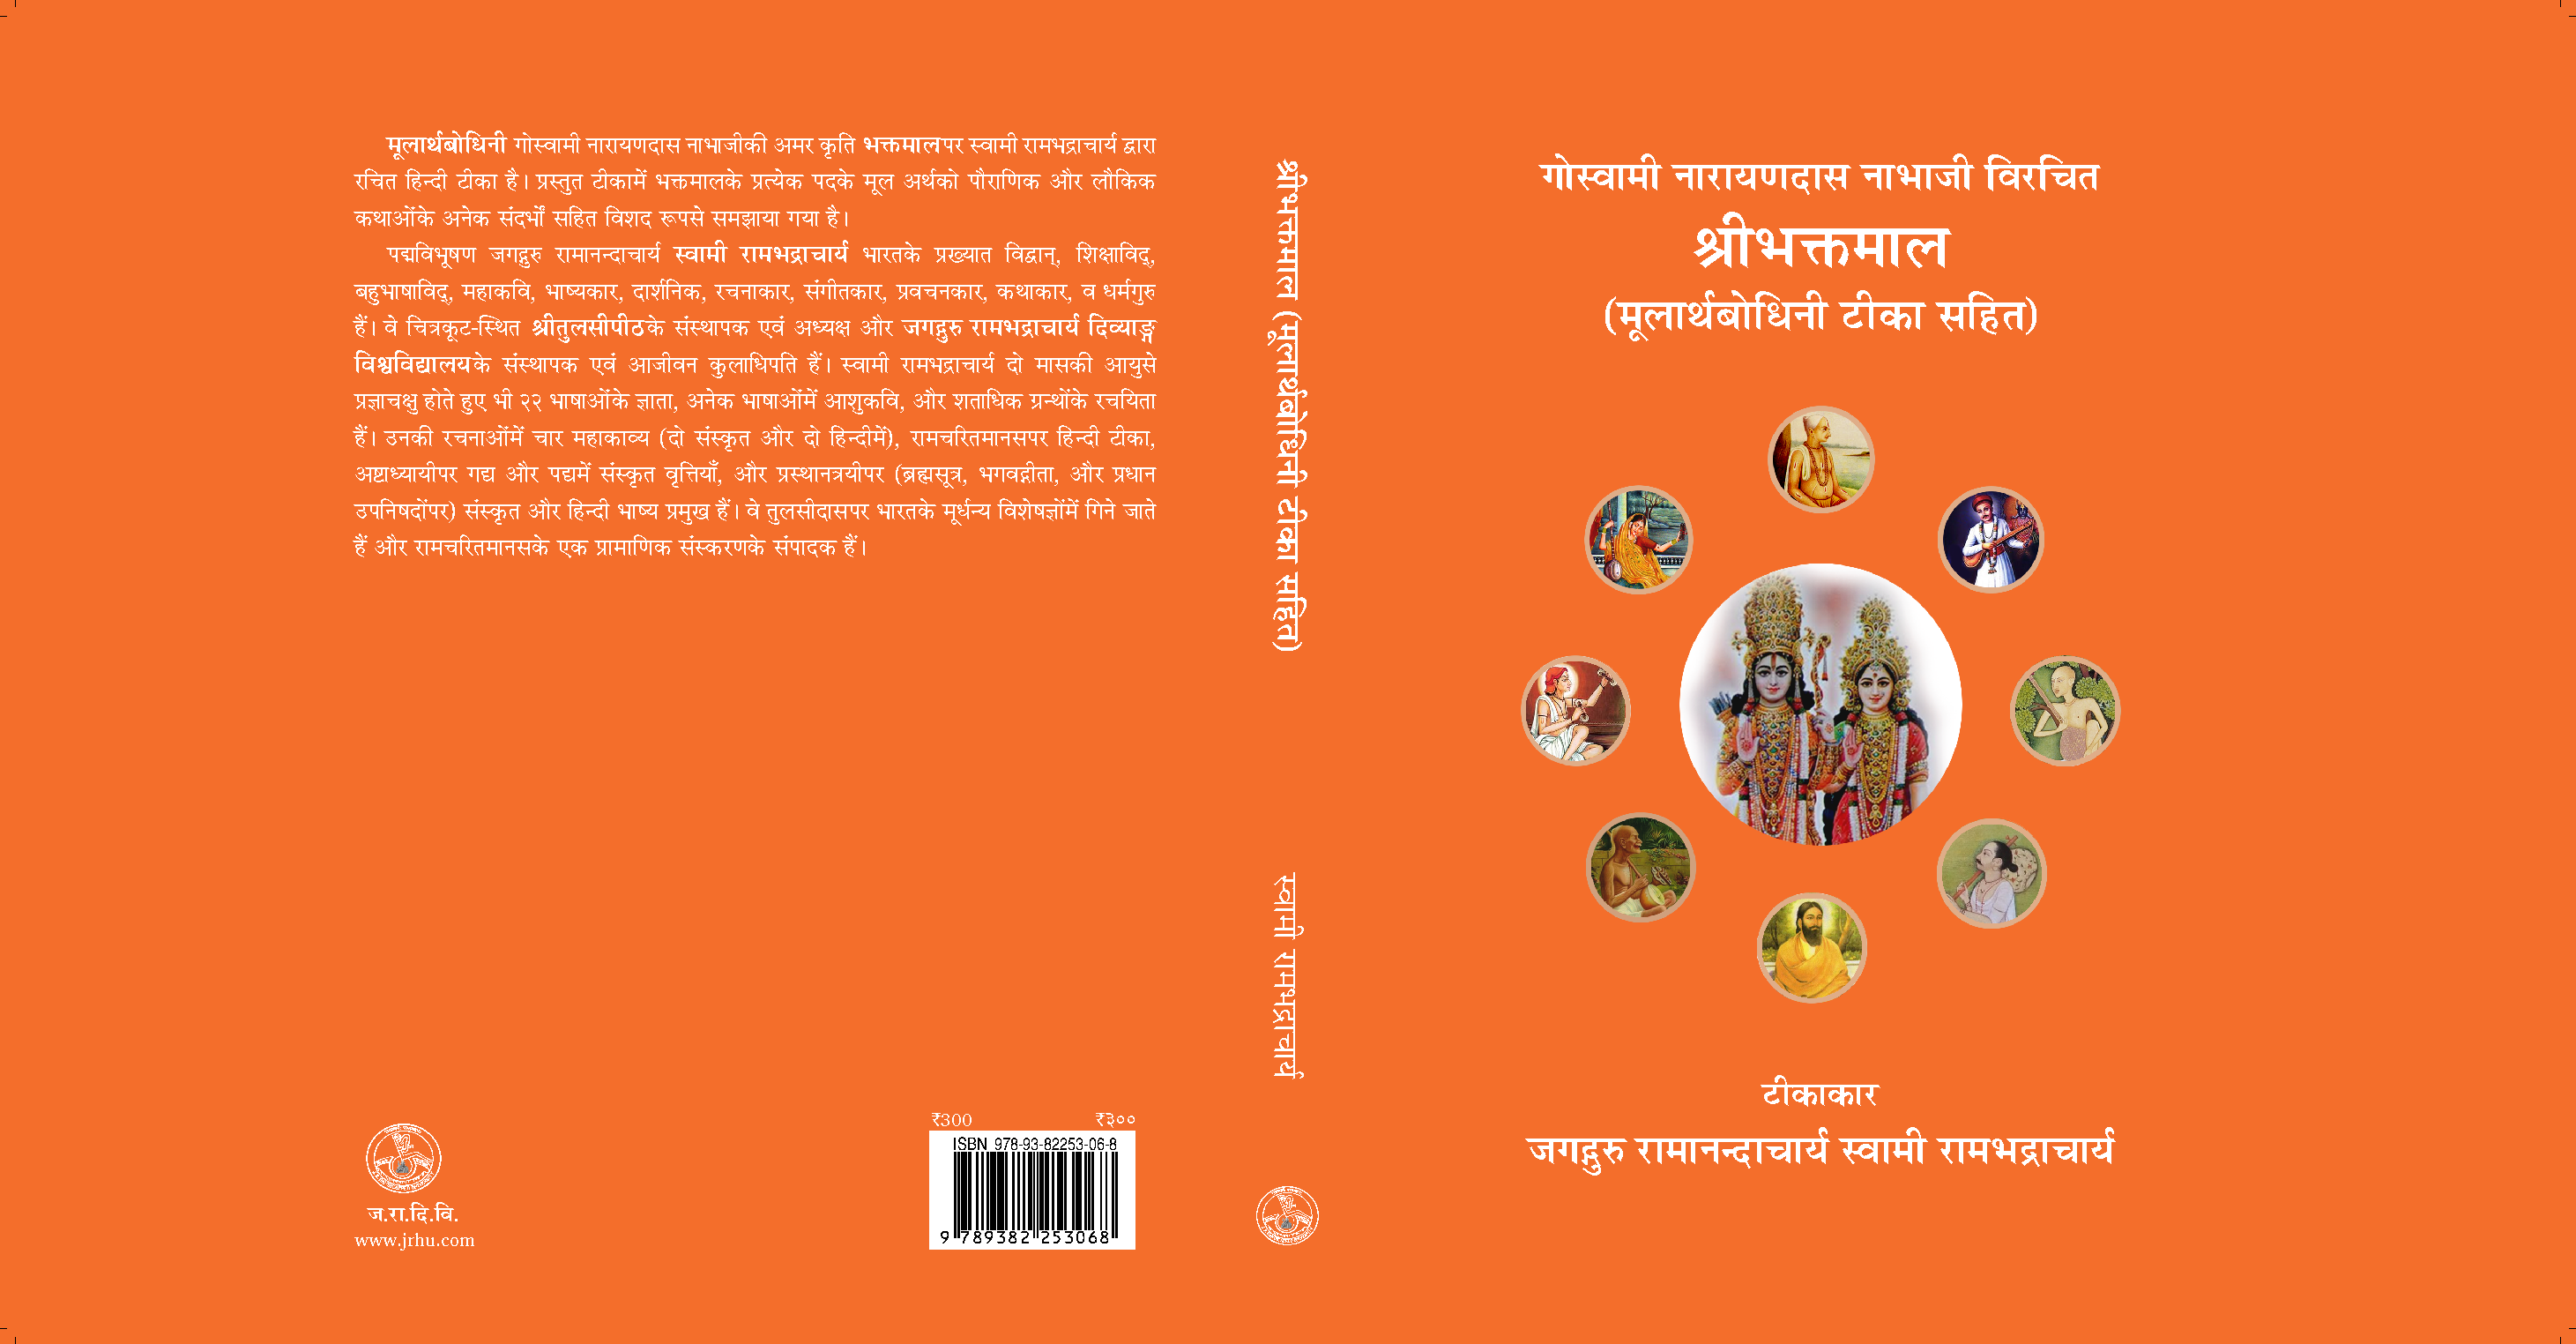
\includepdf[pages=1,trim=257.75mm 3mm 58.75mm 3mm,clip]{DustJacket}

\begin{titlepage}
\thispagestyle{empty}
\begin{center}
\vspace*{4mm}
{\fontsize{20}{24}\selectfont \textbf{श्रीभक्तमाल—मूलार्थबोधिनी टीका सहित}}\\
\end{center}
\cleardoublepage
\thispagestyle{empty}
\begin{center}
\vspace*{4.5mm}
{\fontsize{26}{39}\selectfont \textbf{गोस्वामी नारायणदास नाभाजी विरचित}}\\
\vspace*{3mm}
{\fontsize{36}{54}\selectfont \textbf{श्रीभक्तमाल}}\\
\vspace*{4.5mm}
{\fontsize{28}{42}\selectfont \textbf{(मूलार्थबोधिनी टीका सहित)}}\\
\vfill
{\fontsize{18}{27}\selectfont टीकाकार}\\
\vspace*{2.5mm}
{\fontsize{18}{27}\selectfont धर्मचक्रवर्ती महामहोपाध्याय कविकुलरत्न वाचस्पति पद्मविभूषण-विभूषित}\\
\vspace*{1mm}
{\fontsize{18}{27}\selectfont महाकवि श्रीचित्रकूटतुलसीपीठाधीश्वर जगद्गुरु रामानन्दाचार्य}\\
\vspace*{1mm}
{\fontsize{26}{39}\selectfont \textbf{स्वामी रामभद्राचार्य}}\\
\vspace*{2.5mm}
{\fontsize{16}{22}\selectfont जीवन पर्यन्त कुलाधिपति}\\
\vspace*{1mm}
{\fontsize{16}{22}\selectfont जगद्गुरु रामभद्राचार्य दिव्याङ्ग विश्वविद्यालय, चित्रकूट}\\
\vfill
{\fontsize{16}{24}\selectfont द्वितीय संस्करण}\\
\vspace*{2.5mm}
\vfill
{\fontsize{16}{24}\selectfont प्रकाशक}\\
\vspace*{2.5mm}
%\vspace*{1mm}
{\fontsize{18}{27}\selectfont जगद्गुरु रामभद्राचार्य दिव्याङ्ग विश्वविद्यालय, चित्रकूट}\\
\vspace*{2.5mm}
{\fontsize{18}{27}\selectfont विक्रम संवत् २०७७}
\vspace*{4.5mm}
\end{center}
\pagebreak
\thispagestyle{empty}
\begin{center}
\vspace*{3.5mm}
{\fontsize{15}{22.5}\selectfont \textbf{प्रकाशक}}\\
\vspace*{1.25mm}
{\fontsize{15}{22.5}\selectfont जगद्गुरु रामभद्राचार्य  दिव्याङ्ग विश्वविद्यालय}\\
\vspace*{0.5mm}
{\fontsize{15}{22.5}\selectfont कर्वी, चित्रकूट, उत्तरप्रदेश २१०२०४, भारत}\\
\vspace*{0.5mm}
{\englishfont \fontsize{11}{22.5}\selectfont www.jrhu.com}\\
\vfill
{\fontsize{15}{22.5}\selectfont प्रथम संस्करण: चित्रकूट, विक्रम संवत् २०७० (जनवरी २०१४)}\\
\vspace*{1mm}
{\fontsize{15}{22.5}\selectfont द्वितीय संस्करण: चित्रकूट, विक्रम संवत् २०७७ (जनवरी २०२१)}\\
\vfill
{\fontsize{15}{22.5}\selectfont न्यौछावर: ३०० रुपये मात्र}\\
\vfill
{\englishfont \fontsize{12}{13}\selectfont © }{\fontsize{15}{17.5}\selectfont २०१४–२०२१ स्वामी रामभद्राचार्य}\\
\vfill
{\englishfont \fontsize{11}{13}\selectfont ISBN-13: 978-93-82253-06-8}\\
\vspace*{2.5mm}
{\englishfont \fontsize{11}{13}\selectfont ISBN-10: 93-82253-06-8}\\
\vfill
\vfill
{\fontsize{15}{17.5}\selectfont \textbf{चाणक्यसंस्कृत}में %और {\englishfont {\relscale{0.8} \textbf{Charis SIL}}}
 अक्षर-संयोजन: नित्यानन्द मिश्र}\\
\vfill
{\fontsize{15}{17.5}\selectfont \textbf{मुद्रक}}\\{\englishfont \fontsize{11}{15}\selectfont Dhote Offset Technokrafts Pvt. Ltd.\\C/203 Sintofine Industrial Estate\\Vishweshwar Nagar Road, Goregaon (East)\\Mumbai 400063, India\\}
\vspace*{3.5mm}
\end{center}
\end{titlepage}

\mbox{}
\thispagestyle{empty}
\newpage
\mbox{}
\thispagestyle{empty}
\newpage


%\addcontentsline{toc}{chapter}{संकेताक्षर-सूची}
\chapter*{संकेताक्षर-सूची}
\thispagestyle{empty}
\fontsize{16}{19}\selectfont
\begin{longtable}{p{30mm}l}
% This file is part of Mūlārthabodhinī XeLaTeX Source Code
% Mūlārthabodhinī XeLaTeX Source Code is free software: you can redistribute it and/or modify it under the terms of the GNU General Public License as published by the Free Software Foundation, either version 3 of the License, or (at your option) any later version.
% Mūlārthabodhinī XeLaTeX Source Code is distributed in the hope that it will be useful, but WITHOUT ANY WARRANTY; without even the implied warranty of MERCHANTABILITY or FITNESS FOR A PARTICULAR PURPOSE. See the GNU General Public License for more details.
% You should have received a copy of the GNU General Public License along with Mūlārthabodhinī XeLaTeX Source Code. If not, see <https://www.gnu.org/licenses/>.
अ.को. & अमरकोष\\[1mm]
अ.सं.प. & अगस्त्य संहिता परिशिष्ट\\[1mm]
ई.उ.शा.पा. & ईशावास्य उपनिषद् शान्तिपाठ\\[1mm]
क. & कवितावली\\[1mm]
कृ.क.अ. & कृष्णकर्णामृत\\[1mm]
ग.सं. & गर्गसंहिता\\[1mm]
गी. & गीतावली\\[1mm]
गी.गो. & गीतगोविन्द\\[1mm]
च.प.स्तो. & चर्पटपञ्जरिकास्तोत्र\\[1mm]
ज.अ. & जगन्नाथाष्टक\\[1mm]
तु.स.स. & तुलसी सतसई\\[1mm]
दु.स.श. & दुर्गासप्तशती\\[1mm]
दो. & दोहावली\\[1mm]
नी.श. & नीतिशतक\\[1mm]
पा.गी. & पाण्डव गीता\\[1mm]
पा.सू. & पाणिनि सूत्र (अष्टाध्यायी)\\[1mm]
ब.रा. & बरवै रामायण \\[1mm]
भ.गी. & श्रीमद्भगवद्गीता\\[1mm]
भ.पु.प्रति.प. & भविष्यपुराण प्रतिसर्गपर्व\\[1mm]
भ.मा. & भक्तमाल\\[1mm]
भ.र.बो. & भक्तिरसबोधिनी (प्रियादासजीकृत भक्तमालटीका)\\[1mm]
भ.र.सि. & भक्तिरसामृतसिन्धु\\[1mm]
भा.पु. & श्रीमद्भागवतपुराण\\[1mm]
भा.पु.श्री.टी. & श्रीमद्भागवतपुराण श्रीधरटीका \\[1mm]
भा.पु.श्री.टी.म. & श्रीमद्भागवतपुराण श्रीधरटीका मङ्गलाचरण \\[1mm]
म.स्मृ. & मनुस्मृति\\[1mm]
मा. & श्रीरामचरितमानस\\[1mm]
मा.पु. & मार्कण्डेय पुराण\\[1mm]
मु.उ. & मुण्डक उपनिषद्\\[1mm]
मे.को.धा.व. & मेदिनीकोष धान्तवर्ग\\[1mm]
र.वं. & रघुवंश \\[1mm]
रा.र.स्तो. & रामरक्षास्तोत्र\\[1mm]
वा.रा. & वाल्मीकीय रामायण \\[1mm]
वि.प. & विनयपत्रिका \\[1mm]
वि.पु. & विष्णुपुराण\\[1mm]
वै.म.भा. & वैष्णवमताब्जभास्कर\\[1mm]
स्क.पु.ब्र.ख.ध.मा. & स्कन्दपुराण ब्रह्मखण्ड धर्मारण्यमाहात्म्य \\[1mm]
स्क.पु.रे.ख.स.क. & स्कन्दपुराण रेवाखण्ड सत्यनारायणकथा\\[1mm]
ह.बा. & हनुमान बाहुक \\[1mm]
हि. & हितोपदेश\\[1mm]
हि.प्र. & हितोपदेश प्रस्तावना\\[1mm]

\end{longtable}
\vspace*{2.5mm}
\paraseplotus
\cleardoublepage

\fontsize{14}{15.75}\selectfont

% \renewcommand{\contentsname}{विषय-सूची}
\renewcommand{\contentsname}{\hfill विषय-सूची \hfill}   
\renewcommand{\cftaftertoctitle}{\hfill}
{\pdfbookmark[0]{विषय-सूची}{}
\fancyhead[RE,LO]{}
\fancyhead[LE,RO]{}
\setlength\cftbeforechapskip{4mm}
\setlength\cftbeforesecskip{2mm}
\setlength\cftaftertoctitleskip{0pt}
\tableofcontents
\paraseplotus
\cleardoublepage}

\fancyhead[RO,LE]{\textmd{\Large(\thepage)}}

\mainmatter
\renewcommand\cftchappagefont{\fontsize{16}{21}\selectfont\devfont\bfseries}
\renewcommand{\thepage}{\mdseries\devanagarinumeral{page}}

\setcounter{footnote}{0}
\justifying
\phantomsection
\addcontentsline{toc}{chapter}{संपादकीय}
\chapter*{संपादकीय}
\thispagestyle{empty}
\fancyhead[CO]{{\textmd{\Large श्रीभक्तमाल (मूलार्थबोधिनी)}}}
\fancyhead[CE]{{\textmd{\Large संपादकीय}}}
\fontsize{16}{21}\selectfont
% This file is part of Mūlārthabodhinī XeLaTeX Source Code

% Mūlārthabodhinī XeLaTeX Source Code is free software: you can redistribute it and/or modify it under the terms of the GNU General Public License as published by the Free Software Foundation, either version 3 of the License, or (at your option) any later version.

% Mūlārthabodhinī XeLaTeX Source Code is distributed in the hope that it will be useful, but WITHOUT ANY WARRANTY; without even the implied warranty of MERCHANTABILITY or FITNESS FOR A PARTICULAR PURPOSE. See the GNU General Public License for more details.

% You should have received a copy of the GNU General Public License along with Mūlārthabodhinī XeLaTeX Source Code. If not, see <https://www.gnu.org/licenses/>.

\begin{sloppypar}\justifying\hyphenrules{nohyphenation}
प्रस्तुत ग्रन्थके प्रथम संस्करणकी सभी प्रतियोंका अल्प समयमें समाप्त हो जाना इस पुस्तककी लोकप्रियताका सूचक है। गुरुदेव ने इस वर्षके प्रारम्भमें इसके पुनर्मुद्रणका संकल्प लिया था, परन्तु वैश्विक महामारी कोरोनाके कारण मुद्रणमें विलम्ब हो गया। द्वितीय संस्करण नए फ़ॉण्टमें संयोजित है और मुम्बईसे छपा है। प्रथम संस्करणमें टङ्कणकी कुछ अशुद्धियोंका निवारण किया गया है, जिसमें श्रीमोहन गर्गने महत्त्वपूर्ण योगदान दिया है। श्रीरामाधार शर्मा और श्रीमनीषकुमार शुक्लके मार्गदर्शनके बिना यह ग्रन्थ पुनः पुस्तकाकार न हो पाता। प्रथम संस्करणकी भाँति यह संस्करण भी भक्तों और पाठकोंको सविनय समर्पित है।
\end{sloppypar}

{\bfseries
\setlength{\mylenone}{0pt}
\settowidth{\mylentwo}{नूतनं वर्ष्म संप्राप्ता द्वैतीयीकतया मितम्}
\setlength{\mylenone}{\maxof{\mylenone}{\mylentwo}}
\settowidth{\mylentwo}{मूलार्थबोधिनी टीका भक्तमालस्य राजते}
\setlength{\mylenone}{\maxof{\mylenone}{\mylentwo}}
\setlength{\mylentwo}{\baselineskip}
\setlength{\mylenone}{\mylenone + 1pt}
\setlength{\mylen}{(\textwidth - \mylenone)*\real{0.5}}
\begin{longtable}[l]{@{\hspace*{\mylen}}>{\setlength\parfillskip{0pt}}p{\mylenone}@{}@{}l@{}}
 & \\[-\the\mylentwo]
नूतनं वर्ष्म संप्राप्ता द्वैतीयीकतया मितम् & ।\\ \nopagebreak
मूलार्थबोधिनी टीका भक्तमालस्य राजते & ॥
\end{longtable}
}

\raggedleft{इति निवेदयति\nopagebreak\\
नित्यानन्द मिश्र\nopagebreak\\}
\begin{sloppypar}\justifying\hyphenrules{nohyphenation}
\noindent मकर संक्रान्ति\nopagebreak\\
विक्रम संवत् २०७७
\end{sloppypar}
\paraseplotus

\addcontentsline{toc}{chapter}{संपादकीय~(प्रथम~संस्करण)}
\chapter*{संपादकीय~(प्रथम~संस्करण)}
% This file is part of Mūlārthabodhinī XeLaTeX Source Code

% Mūlārthabodhinī XeLaTeX Source Code is free software: you can redistribute it and/or modify it under the terms of the GNU General Public License as published by the Free Software Foundation, either version 3 of the License, or (at your option) any later version.

% Mūlārthabodhinī XeLaTeX Source Code is distributed in the hope that it will be useful, but WITHOUT ANY WARRANTY; without even the implied warranty of MERCHANTABILITY or FITNESS FOR A PARTICULAR PURPOSE. See the GNU General Public License for more details.

% You should have received a copy of the GNU General Public License along with Mūlārthabodhinī XeLaTeX Source Code. If not, see <https://www.gnu.org/licenses/>.

\fontsize{16}{21}\selectfont

{\bfseries
\setlength{\mylenone}{0pt}
\settowidth{\mylentwo}{रामभद्र गुरुदेव पर कृपा भक्त हरि की परी}
\setlength{\mylenone}{\maxof{\mylenone}{\mylentwo}}
\settowidth{\mylentwo}{मानस को कल हंस भक्तकुल बारिधि सितकर}
\setlength{\mylenone}{\maxof{\mylenone}{\mylentwo}}
\settowidth{\mylentwo}{बिबुध राष्ट्र ब्रज गिरा दच्छ कबिकमल दिवाकर}
\setlength{\mylenone}{\maxof{\mylenone}{\mylentwo}}
\settowidth{\mylentwo}{ब्रह्मसूत्र उपनिषद भाष्यकर गीता मधुकर}
\setlength{\mylenone}{\maxof{\mylenone}{\mylentwo}}
\settowidth{\mylentwo}{गानबिधा गंधर्ब सकल बिद्या को आकर}
\setlength{\mylenone}{\maxof{\mylenone}{\mylentwo}}
\settowidth{\mylentwo}{मूल अर्थ बोधिनि ललित भक्तमाल टीका करी}
\setlength{\mylenone}{\maxof{\mylenone}{\mylentwo}}
\settowidth{\mylentwo}{रामभद्र गुरुदेव पर कृपा भक्त हरि की परी}
\setlength{\mylenone}{\maxof{\mylenone}{\mylentwo}}
\setlength{\mylentwo}{\baselineskip}
\setlength{\mylenone}{\mylenone + 1pt}
\setlength{\mylen}{(\textwidth - \mylenone)*\real{0.5}}
\begin{longtable}[l]{@{\hspace*{\mylen}}>{\setlength\parfillskip{0pt}}p{\mylenone}@{}@{}l@{}}
 & \\[-\the\mylentwo]
रामभद्र गुरुदेव पर कृपा भक्त हरि की परी & ॥\\ \nopagebreak
मानस को कल हंस भक्तकुल बारिधि सितकर & ।\\ \nopagebreak
बिबुध राष्ट्र ब्रज गिरा दच्छ कबिकमल दिवाकर & ॥\\
ब्रह्मसूत्र उपनिषद भाष्यकर गीता मधुकर & ।\\ \nopagebreak
गानबिधा गंधर्ब सकल बिद्या को आकर & ॥\\
मूल अर्थ बोधिनि ललित भक्तमाल टीका करी & ।\\ \nopagebreak
रामभद्र गुरुदेव पर कृपा भक्त हरि की परी & ॥\\
\end{longtable}
}

\begin{sloppypar}\justifying\hyphenrules{nohyphenation}
गोस्वामी श्रीनारायणदास नाभाजीद्वारा विरचित श्रीभक्तमाल भारतीय भक्तिपरम्पराकी एक अमूल्य निधि होनेके साथ-साथ भारतीय भाषा\-साहित्यका एक अग्रगण्य सारस्वत पुष्प भी है। लौकिक मालामें पुष्पों अथवा रत्नोंका, सूत्रका, सुमेरुका और फुँदनेका अपना-अपना महत्त्व है—और इन चारोंके रुचिकर संयोगसे ही आकर्षक मालाका निर्माण संभव है। श्रीभक्तमाल ऐसी दिव्य माला है जिसमें भक्तगण ही पुष्प अथवा रत्न हैं, परमप्रेमरूपा अमृतस्वरूपा भक्ति ही सूत्र है, गोस्वामी तुलसीदास सरीखे गुरूपम संत अथवा भक्तिसिद्धान्तका दान देनेवाले सद्गुरुदेव ही सुमेरु हैं, और स्वयं पद्मपत्राक्ष श्रीरामकृष्णनारायणाभिन्न भगवान् ही फुँदना हैं। चारों ही श्रेष्ठ हैं और भक्तमालकार अपने प्रथम दोहेमें ही चारोंको अभिन्न बताते हैं, यथा—
\end{sloppypar}

{\bfseries
\setlength{\mylenone}{0pt}
\settowidth{\mylentwo}{भक्त भक्ति भगवंत गुरु चतुर नाम बपु एक}
\setlength{\mylenone}{\maxof{\mylenone}{\mylentwo}}
\setlength{\mylentwo}{\baselineskip}
\setlength{\mylenone}{\mylenone + 1pt}
\setlength{\mylen}{(\textwidth - \mylenone)*\real{0.5}}
\begin{longtable}[l]{@{\hspace*{\mylen}}>{\setlength\parfillskip{0pt}}p{\mylenone}@{}@{}l@{}}
 & \\[-\the\mylentwo]
भक्त भक्ति भगवंत गुरु चतुर नाम बपु एक & ।\\ \nopagebreak
\caption*{(भ.मा.~१)}
\end{longtable}
}

\begin{sloppypar}\justifying\hyphenrules{nohyphenation}
तथापि मालाका नामकरण तो पुष्पों अथवा रत्नोंके आधारपर ही होता है, यथा वनमाला, वैजयन्तीमाला, तुलसीमाला, मणिरत्नमाला, इत्यादि। इसीलिये इस ललित कृतिका नाम नाभाजीने \textbf{भक्तमाल} रखा है।
\end{sloppypar}
\begin{sloppypar}\justifying\hyphenrules{nohyphenation}
एक-साथ भक्तमालके मूलपाठके सरल अर्थों और गूढ भावोंको प्रकाशित करने वाली गुरुदेव जगद्गुरु रामानन्दाचार्य स्वामी रामभद्राचार्यद्वारा प्रणीत \textbf{मूलार्थबोधिनी टीका}का प्रथम संस्करण पाठकोंके समक्ष प्रस्तुत करते हुए हम अनिर्वचनीय कृतकृत्यताका अनुभव कर रहे हैं। विगत मास अर्थात् दिसम्बर २०१३में ही इस विशद टीकाका ऋतम्भराप्रज्ञासंपन्न गुरुदेवने मात्र पन्द्रह घण्टोंमें प्रणयन किया। यह कोई आश्चर्यका विषय नहीं, अपितु माता सरस्वतीके अनुग्रह और प्रभु श्रीसीतारामकी कृपाका प्रत्यक्ष प्रमाण है। जैसे गुरु श्रीअग्रदेवजीके आशीर्वादसे अनेकानेक भूत, वर्तमान और भावी भक्तोंके चरित्र श्रीनाभाजीके हृदयमें स्वतः प्रकाशित हो गए थे, उसी प्रकार रामानन्द संप्रदायकी आद्यगुरु भगवती सीताजीके आशीर्वादसे नाभाजी द्वारा गुम्फित अक्षरोंके मूलार्थ गुरुदेवके हृदयमें स्वतः स्फुरित हुए हैं। स्वयं गुरुदेवने छठे पदकी टीकामें कहा है कि प्रभु श्रीरामके चरणोंमें अन्य टीकाकारोंके मतानुसार २२ नहीं अपितु २४ चिह्न उनके ध्यानमें स्फुरित हुए हैं, जिनका वर्णन नाभाजीने किया है। मूलार्थबोधिनीके अनुशीलनके समय अनेक स्थानोंपर पाठकगण भगवदीय प्रेरणासे हुई इस दिव्य स्फुरणाका अनुभव करेंगे ही।
\end{sloppypar}
\begin{sloppypar}\justifying\hyphenrules{nohyphenation}
अस्तु। प्रणयनके पश्चात् इस टीकाका केवल दो सप्ताहोंमें पुस्तकाकार होना भी श्रीराघवकृपा और गुरुकृपाका ही परिणाम है। टीकाके प्रकाशनमें अत्यन्त महनीय योगदान दिया है हापुड़निवासी श्रीमोहन गर्गजीने। यह एक दिव्य संयोग है कि श्रीमोहन गर्गजीने मूलार्थबोधिनीके प्रणयनकी समाप्तिके दिन ही गुरुदेवसे मन्त्रदीक्षा ली है, यद्यपि गुरुदेवकी सारस्वत सेवा वे पहलेसे करते आए हैं। श्रीमोहन गर्गजीने बड़ी ही दक्षताके साथ ग्रन्थके टङ्कण और लिपिपरिमार्जनमें जो योगदान दिया है, उसके बिना कदाचित् ही यह संस्करण इतने अल्प समयमें मुद्रित हो पाता। आवरण पृष्ठका प्रारूप तैयार किया है गुजरातके रहनेवाले और बेंगलूरुमें सेवारत श्रीमौलिक सूचकजीने। पुस्तकका मुद्रण कानपुरनिवासी श्रीअजय वर्माके \textbf{नीलम मुद्रणालय}में हुआ है, जहाँसे पिछले वर्ष गुरुदेव कृत श्रीहनुमानचालीसाकी \textbf{महावीरी व्याख्या} छपी थी।
\end{sloppypar}
\begin{sloppypar}\justifying\hyphenrules{nohyphenation}
प्रस्तुत संस्करणमें भक्तमालका मूलपाठ संपादकोंने यथामति भिन्न-भिन्न संस्करणोंके आधारपर लिया है। भक्तमालका कोई प्रामाणिक संस्करण हमें इस समयमें उपलब्ध न हो पाया, और हमारे द्वारा संदर्भित संस्करणोंमें कुछ स्थानोंपर पाठभेद हैं। फलस्वरूप पाठकोंको कुछ स्थलोंपर प्रचलित प्रति से पाठभेद मिल सकता है। भक्तमालपर सुविशाल \textbf{भक्तकृपाभाष्य} गुरुदेवका संकल्प है, और हमारी आशा है कि गुरुदेव द्वारा भक्तकृपाभाष्यके प्रणयनके साथ-साथ भक्तमालके प्रामाणिक पाठका संपादन भी होगा।
\end{sloppypar}
\begin{sloppypar}\justifying\hyphenrules{nohyphenation}
संभव है प्रस्तुत संस्करणमें संपादकीय त्रुटियाँ रह गईं हों। यदि ऐसा हुआ है तो पाठक भक्त उन्हें हम अल्पज्ञ संपादकोंके मानवजन्य भ्रम, प्रमाद, विप्रलिप्सा और करणापाटवका परिणाम समझकर हमें क्षमा करें और शीघ्रातिशीघ्र वैद्युत\-पत्राचार ({\englishfont{\relscale{0.77}e-mail}}) द्वारा {\englishfont{\relscale{0.77}namoraghavay@gmail.com}} पतेपर सूचित करें ताकि पुस्तकके अन्तर्जाल संस्करण ({\englishfont{\relscale{0.77}online edition}}) और आगामी मुद्रित संस्करणोंमें उनका निवारण हो सके।
\end{sloppypar}
\begin{sloppypar}\justifying\hyphenrules{nohyphenation}
हम गुरुदेवकी इस मनोहारिणी टीकाको भक्तों और पाठकोंको विनीत भावसे समर्पित करते हैं और प्रार्थना करते हैं कि—
\end{sloppypar}

{\bfseries
\setlength{\mylenone}{0pt}
\settowidth{\mylentwo}{गायं गायं भक्तमालं सरागं पाठं पाठं रामभद्रार्यटीकाम्}
\setlength{\mylenone}{\maxof{\mylenone}{\mylentwo}}
\settowidth{\mylentwo}{स्मारं स्मारं भक्तपादाब्जधूलिं जीवा लोके भूरिभाग्या भवन्तु}
\setlength{\mylenone}{\maxof{\mylenone}{\mylentwo}}
\setlength{\mylentwo}{\baselineskip}
\setlength{\mylenone}{\mylenone + 1pt}
\setlength{\mylen}{(\textwidth - \mylenone)*\real{0.5}}
\begin{longtable}[l]{@{\hspace*{\mylen}}>{\setlength\parfillskip{0pt}}p{\mylenone}@{}@{}l@{}}
 & \\[-\the\mylentwo]
गायं गायं भक्तमालं सरागं पाठं पाठं रामभद्रार्यटीकाम् & ।\\ \nopagebreak
स्मारं स्मारं भक्तपादाब्जधूलिं जीवा लोके भूरिभाग्या भवन्तु & ॥
\end{longtable}
}

\raggedleft{इति निवेदयन्ति\nopagebreak\\
भक्तानां वशंवदाः\nopagebreak\\
डॉ. रामाधार शर्मा\nopagebreak\\
नित्यानन्द मिश्र\nopagebreak\\
मनीषकुमार शुक्ल\nopagebreak\\}
\begin{sloppypar}\justifying\hyphenrules{nohyphenation}
\noindent मकर संक्रान्ति\nopagebreak\\
विक्रम संवत् २०७०
\end{sloppypar}
\paraseplotus

\cleardoublepage


\setcounter{footnote}{0}
\justifying
\phantomsection
\addcontentsline{toc}{chapter}{प्राक्कथन}
\chapter*{प्राक्कथन}
\thispagestyle{empty}
\fancyhead[CO]{{\textmd{\Large श्रीभक्तमाल (मूलार्थबोधिनी)}}}
\fancyhead[CE]{{\textmd{\Large प्राक्कथन}}}
% This file is part of Mūlārthabodhinī XeLaTeX Source Code

% Mūlārthabodhinī XeLaTeX Source Code is free software: you can redistribute it and/or modify it under the terms of the GNU General Public License as published by the Free Software Foundation, either version 3 of the License, or (at your option) any later version.

% Mūlārthabodhinī XeLaTeX Source Code is distributed in the hope that it will be useful, but WITHOUT ANY WARRANTY; without even the implied warranty of MERCHANTABILITY or FITNESS FOR A PARTICULAR PURPOSE. See the GNU General Public License for more details.

% You should have received a copy of the GNU General Public License along with Mūlārthabodhinī XeLaTeX Source Code. If not, see <https://www.gnu.org/licenses/>.

{\bfseries
\setlength{\mylenone}{0pt}
\settowidth{\mylentwo}{श्रीमद्ब्रह्मसमारम्भां सम्प्रदायार्यमध्यमाम्}
\setlength{\mylenone}{\maxof{\mylenone}{\mylentwo}}
\settowidth{\mylentwo}{श्रीलालमतीपर्यन्तां वन्दे भक्तपरम्पराम्}
\setlength{\mylenone}{\maxof{\mylenone}{\mylentwo}}
\setlength{\mylentwo}{\baselineskip}
\setlength{\mylenone}{\mylenone + 1pt}
\setlength{\mylen}{(\textwidth - \mylenone)*\real{0.5}}
\begin{longtable}[l]{@{\hspace*{\mylen}}>{\setlength\parfillskip{0pt}}p{\mylenone}@{}@{}l@{}}
 & \\[-\the\mylentwo]
श्रीमद्ब्रह्मसमारम्भां सम्प्रदायार्यमध्यमाम् & ।\\ \nopagebreak
श्रीलालमतीपर्यन्तां वन्दे भक्तपरम्पराम् & ॥
\end{longtable}
}

\begin{sloppypar}\justifying\hyphenrules{nohyphenation}
श्रीअग्रदास(अग्रदेवाचार्यजी)के सुयोग्य, भगवत्साक्षात्कारी, अन्तस्तलपर्यन्त प्रवेश करनेवाले शिष्य श्रीनारायणदास गोस्वामी नाभाजी कृत श्रीभक्तमालको आज कौन नहीं जानता? और यूँ कहें तो कोई अतिरञ्जना नहीं होगी कि श्रीरामचरितमानसके पश्चात् यदि हिन्दी साहित्यमें किसीको भाषा\-सौष्ठव, काव्यचातुरी, संप्रेषण\-शीलता एवं भगवद्गुणगानके नैपुण्यका विरुद प्राप्त है तो वे हैं १००८~श्रीनारायणदास गोस्वामी नाभाजी महाराजके द्वारा कृत श्रीभक्तमालजी। यहाँ यह भी कहना असाम्प्रतिक नहीं होगा कि गोस्वामी तुलसीदासजी कृत श्रीरामचरितमानसजीके प्राकट्यके पश्चात् तत्काल ही श्रीभक्तमालजीका आविर्भाव हो चुका था, क्योंकि श्रीभक्तमालके सुमेरुके रूपमें गोस्वामी तुलसीदासजीको ही नाभाजीने अपने श्रीभक्तमालमें प्रतिष्ठापित किया और यह भी स्पष्ट किया कि उनके श्रीभक्तमालकी रचनाके पूर्व ही श्रीरामचरितमानसजीका प्रणयन हो चुका था। वे कहते हैं—
\end{sloppypar}

{\bfseries
\setlength{\mylenone}{0pt}
\settowidth{\mylentwo}{कलि कुटिल जीव निस्तारहित बाल्मीकि तुलसी भये}
\setlength{\mylenone}{\maxof{\mylenone}{\mylentwo}}
\settowidth{\mylentwo}{त्रेता काब्य निबंध कियो सत कोटि रमायन}
\setlength{\mylenone}{\maxof{\mylenone}{\mylentwo}}
\settowidth{\mylentwo}{इक अच्छर उद्धरे ब्रह्महत्यादि परायन}
\setlength{\mylenone}{\maxof{\mylenone}{\mylentwo}}
\settowidth{\mylentwo}{अब भक्तन सुख देन बहुरि लीला बिस्तारी}
\setlength{\mylenone}{\maxof{\mylenone}{\mylentwo}}
\settowidth{\mylentwo}{रामचरन रसमत्त रहत अहनिसि ब्रतधारी}
\setlength{\mylenone}{\maxof{\mylenone}{\mylentwo}}
\settowidth{\mylentwo}{संसार अपार के पार को सुगम रूप नौका लये}
\setlength{\mylenone}{\maxof{\mylenone}{\mylentwo}}
\settowidth{\mylentwo}{कलि कुटिल जीव निस्तारहित बाल्मीकि तुलसी भये}
\setlength{\mylenone}{\maxof{\mylenone}{\mylentwo}}
\setlength{\mylentwo}{\baselineskip}
\setlength{\mylenone}{\mylenone + 1pt}
\setlength{\mylen}{(\textwidth - \mylenone)*\real{0.5}}
\begin{longtable}[l]{@{\hspace*{\mylen}}>{\setlength\parfillskip{0pt}}p{\mylenone}@{}@{}l@{}}
 & \\[-\the\mylentwo]
कलि कुटिल जीव निस्तारहित बाल्मीकि तुलसी भये & ॥\\ \nopagebreak
त्रेता काब्य निबंध कियो सत कोटि रमायन & ।\\ \nopagebreak
इक अच्छर उद्धरे ब्रह्महत्यादि परायन & ॥\\
अब भक्तन सुख देन बहुरि लीला बिस्तारी & ।\\ \nopagebreak
रामचरन रसमत्त रहत अहनिसि ब्रतधारी & ॥\\
संसार अपार के पार को सुगम रूप नौका लये & ।\\ \nopagebreak
कलि कुटिल जीव निस्तारहित बाल्मीकि तुलसी भये & ॥\\ \nopagebreak
\caption*{(भ.मा.~१२९)}
\end{longtable}
}

\begin{sloppypar}\justifying\hyphenrules{nohyphenation}
यहाँ प्रयुक्त चार भूतकालिक क्रियाओंको देखकर—\textbf{त्रेता काब्य निबंध कियो}, \textbf{बहुरि लीला बिस्तारी}, \textbf{सुगमरूप नौका लये} और \textbf{बाल्मीकि तुलसी भये}—यह स्पष्ट हो जाता है कि श्रीभक्तमालकी रचनाके पूर्व ही श्रीरामचरितमानसजीका गोस्वामीजीके माध्यमसे आविर्भाव हो चुका था। और चूँकि नाभाजीको गोस्वामी तुलसीदासजीके प्रति अत्यन्त श्रद्धा थी, इससे भी यह निश्चित हो जाता है कि श्रीभक्तमालजीकी रचनाप्रकृति श्रीरामचरितमानसजीकी रचनाधर्मितासे बहुत अंशोंमें मिलती-जुलती है। जैसे गोस्वामी तुलसीदासजी अवधी भाषामें रचना करते हुए भी गँवारू अवधी भाषाके प्रयोगके पक्षमें नहीं दिखते, उनकी अवधी भाषा प्राञ्जल, सुसंस्कृत और बहुत परिष्कृत होती है, गोस्वामीजी जायसी की तरह असभ्य शब्दोंका प्रयोग कभी नहीं करते, ठीक उसी प्रकारका स्वभाव श्रीभक्तमालजीके रचनाकार नाभाजीका है। संतोंके नाम जैसे गाँवमें कहे गए, उनको वैसे ही लिखनेमें वे किसी प्रकार हिचकिचाते नहीं हैं, परन्तु उनके गुणोंके प्रस्तुतीकरणमें गोस्वामीजीकी ही भाँति श्रीनाभाजी भी विशुद्ध संस्कृतनिष्ठ शब्दोंका प्रयोग करते हुए दिखते हैं। जैसे गोस्वामी तुलसीदासजी कहीं-कहीं संस्कृत शब्दावलीके प्रयोगमें संकोच नहीं करते, यथा—
\end{sloppypar}

{\bfseries
\setlength{\mylenone}{0pt}
\setlength{\mylenthree}{0pt}
\settowidth{\mylentwo}{हरि अवतार हेतु जेहिं होई}
\setlength{\mylenone}{\maxof{\mylenone}{\mylentwo}}
\settowidth{\mylenfour}{इदमित्थं कहि जात न सोई}
\setlength{\mylenthree}{\maxof{\mylenthree}{\mylenfour}}
\setlength{\mylentwo}{\baselineskip}
\setlength{\mylenone}{\mylenone + 1pt}
\setlength{\mylenfour}{\baselineskip}
\setlength{\mylenthree}{\mylenthree + 1pt}
\setlength{\mylen}{(\textwidth - \mylenone)}
\setlength{\mylen}{(\mylen - \mylenthree)*\real{0.5}}
\setlength{\mylen}{(\mylen - 4pt)}
\begin{longtable}[l]{@{\hspace*{\mylen}}>{\setlength\parfillskip{0pt}}p{\mylenone}@{}@{}l@{\hspace{6pt}}>{\setlength\parfillskip{0pt}}p{\mylenthree}@{}@{}l@{}}
 & & & \\[-\the\mylentwo]
हरि अवतार हेतु जेहिं होई & । & इदमित्थं कहि जात न सोई & ॥\\ \nopagebreak
\caption*{(मा.~१.१२१.२)}
\end{longtable}
}

\begin{sloppypar}\justifying\hyphenrules{nohyphenation}
यहाँ \textbf{इदमित्थं} शब्दका प्रयोग कितना सुन्दर लग रहा है। इसी प्रकार मानसजीके अयोध्याकाण्डके २२५वें दोहेमें गोस्वामी तुलसीदासजी हिन्दीके प्रयोगोंके साथ संस्कृतका सप्तमी बहुवचनान्त प्रयोग करके भी रसभङ्ग नहीं प्रत्युत रसरङ्ग करते हुए दिख रहे हैं—
\end{sloppypar}

{\bfseries
\setlength{\mylenone}{0pt}
\settowidth{\mylentwo}{भरतप्रेम तेहिं समय जस तस कहि सकइ न शेषु}
\setlength{\mylenone}{\maxof{\mylenone}{\mylentwo}}
\settowidth{\mylentwo}{कबिहिं अगम जस ब्रह्मसुख अह मम मलिन जनेषु}
\setlength{\mylenone}{\maxof{\mylenone}{\mylentwo}}
\setlength{\mylentwo}{\baselineskip}
\setlength{\mylenone}{\mylenone + 1pt}
\setlength{\mylen}{(\textwidth - \mylenone)*\real{0.5}}
\begin{longtable}[l]{@{\hspace*{\mylen}}>{\setlength\parfillskip{0pt}}p{\mylenone}@{}@{}l@{}}
 & \\[-\the\mylentwo]
भरतप्रेम तेहिं समय जस तस कहि सकइ न शेषु & ।\\ \nopagebreak
कबिहिं अगम जस ब्रह्मसुख अह मम मलिन जनेषु & ॥\\ \nopagebreak
\caption*{(मा.~२.२२५)}
\end{longtable}
}

\begin{sloppypar}\justifying\hyphenrules{nohyphenation}
यहाँ \textbf{जनेषु} शब्द काव्यमें रसभङ्ग नहीं कर रहा है। इसी प्रकार युद्धकाण्डके दोहा क्रमाङ्क १०४के छन्दमें—
\end{sloppypar}

{\bfseries
\setlength{\mylenone}{0pt}
\settowidth{\mylentwo}{आजन्मते परद्रोह रत पापौघमय तव तनु अयम्}
\setlength{\mylenone}{\maxof{\mylenone}{\mylentwo}}
\settowidth{\mylentwo}{तुमहूँ दियो निज धाम राम नमामि ब्रह्म निरामयम्}
\setlength{\mylenone}{\maxof{\mylenone}{\mylentwo}}
\setlength{\mylentwo}{\baselineskip}
\setlength{\mylenone}{\mylenone + 1pt}
\setlength{\mylen}{(\textwidth - \mylenone)*\real{0.5}}
\begin{longtable}[l]{@{\hspace*{\mylen}}>{\setlength\parfillskip{0pt}}p{\mylenone}@{}@{}l@{}}
 & \\[-\the\mylentwo]
आजन्मते परद्रोह रत पापौघमय तव तनु अयम् & ।\\ \nopagebreak
तुमहूँ दियो निज धाम राम नमामि ब्रह्म निरामयम् & ॥\\ \nopagebreak
\caption*{(मा.~६.१०४.१३)}
\end{longtable}
}

\begin{sloppypar}\justifying\hyphenrules{nohyphenation}
यहाँ \textbf{नमामि, ब्रह्म, निरामयम्}—ये तीनों संस्कृत शब्द कितने रुचिकर लग रहे हैं। इसी प्रकार युद्धकाण्डके ही १०७वें दोहेके छन्दमें गोस्वामीजी कितने सुन्दर संस्कृत शब्द \textbf{किमपि}का प्रयोग कर रहे हैं—\textbf{का देउँ तोहि त्रैलोक महँ कपि किमपि नहिं बानी समा} (मा.~६.१०७.९)। और आगे चलकर—\textbf{रनजीति रिपुदल बन्धुजुत पश्यामि राममनामयम्} (मा.~६.१०७.९)—यहाँ \textbf{पश्यामि, रामम्, अनामयम्}—ये तीनों शब्द संस्कृतके हैं, पर उनसे यहाँ रसभङ्ग नहीं हो रहा है। इसी प्रकार गोस्वामीजीके परःशत संस्कृत प्रयोग हिन्दी प्रयोगोंके साथ रह कर भी काव्यमें न तो रसभङ्ग कर रहे हैं और न ही अनौचित्य। ठीक इसी प्रकारकी प्रकृति श्रीभक्तमालकारकी भी है। वे भी यथावसर संस्कृत प्रयोगोंको श्रीभक्तमालमें स्थान देते हुए संकोचका अनुभव नहीं करते। जैसे पैंतीसवें पदमें रामानन्दाचार्यजीकी पद्धति\-परम्पराको प्रस्तुत करते हुए नाभाजी कहते हैं—\textbf{तस्य राघवानंद भये भक्तनको मानंद} (भ.मा.~३५)। यहाँ \textbf{तस्य} शब्द कितना सुन्दर और कितना रुचिकर लग रहा है। इसी प्रकार जब नाभाजी संतोंके गुणोंका परिचय प्रस्तुत करते हैं तो वे संस्कृत\-समास\-निष्ठ शब्दोंके प्रयोगोंमें भी किसी प्रकारका संकोच नहीं करते। जैसे उनका छिहत्तरवाँ पद द्रष्टव्य है—
\end{sloppypar}

{\bfseries
\setlength{\mylenone}{0pt}
\settowidth{\mylentwo}{श्रीभट्ट सुभट प्रगटे अघट रस रसिकन मनमोद घन}
\setlength{\mylenone}{\maxof{\mylenone}{\mylentwo}}
\settowidth{\mylentwo}{मधुरभाव संबलित ललित लीला सुबलित छबि}
\setlength{\mylenone}{\maxof{\mylenone}{\mylentwo}}
\settowidth{\mylentwo}{निरखत हरषत हृदय प्रेम बरषत सुकलित कबि}
\setlength{\mylenone}{\maxof{\mylenone}{\mylentwo}}
\settowidth{\mylentwo}{भव निस्तारन हेतु देत दृढ़ भक्ति सबनि नित}
\setlength{\mylenone}{\maxof{\mylenone}{\mylentwo}}
\settowidth{\mylentwo}{जासु सुजस ससि उदय हरत अति तम भ्रम श्रम चित}
\setlength{\mylenone}{\maxof{\mylenone}{\mylentwo}}
\settowidth{\mylentwo}{आनंदकंद श्रीनंदसुत श्रीवृषभानुसुता भजन}
\setlength{\mylenone}{\maxof{\mylenone}{\mylentwo}}
\settowidth{\mylentwo}{श्रीभट्ट सुभट प्रगटे अघट रस रसिकन मनमोद घन}
\setlength{\mylenone}{\maxof{\mylenone}{\mylentwo}}
\setlength{\mylentwo}{\baselineskip}
\setlength{\mylenone}{\mylenone + 1pt}
\setlength{\mylen}{(\textwidth - \mylenone)*\real{0.5}}
\begin{longtable}[l]{@{\hspace*{\mylen}}>{\setlength\parfillskip{0pt}}p{\mylenone}@{}@{}l@{}}
 & \\[-\the\mylentwo]
श्रीभट्ट सुभट प्रगटे अघट रस रसिकन मनमोद घन & ॥\\ \nopagebreak
मधुरभाव संबलित ललित लीला सुबलित छबि & ।\\ \nopagebreak
निरखत हरषत हृदय प्रेम बरषत सुकलित कबि & ॥\\
भव निस्तारन हेतु देत दृढ़ भक्ति सबनि नित & ।\\ \nopagebreak
जासु सुजस ससि उदय हरत अति तम भ्रम श्रम चित & ॥\\
आनंदकंद श्रीनंदसुत श्रीवृषभानुसुता भजन & ।\\ \nopagebreak
श्रीभट्ट सुभट प्रगटे अघट रस रसिकन मनमोद घन & ॥\\ \nopagebreak
\caption*{(भ.मा.~७६)}
\end{longtable}
}

\begin{sloppypar}\justifying\hyphenrules{nohyphenation}
एवंविध शताधिक संस्कृत प्रयोग श्रीभक्तमालमें उपस्थित होकर उसकी रचनाधर्मितामें चार चाँद लगा देते हैं। श्रीभक्तमालकी भाषा \textbf{काव्यभाषा} है, जो भक्तिकालमें प्रसिद्ध थी। यहाँ काव्यभाषा कहनेका मेरा तात्पर्य यह है कि भक्तिकालमें भक्तिकवियोंने एक ऐसी काव्यभाषाका निर्माण किया था, जो अवधी और ब्रज दोनोंका मिश्रण थी। वह न तो केवल अवधी थी और न केवल ब्रज। हाँ, इतना अन्तर अवश्य है कि जो कवि जिस क्षेत्रमें उत्पन्न हुआ उस क्षेत्रकी भाषाका उसपर उतना अधिक प्रभाव पड़ा, यद्यपि सबकी काव्यभाषा एक ही थी। जैसे गोस्वामी तुलसीदासजीकी काव्यभाषा यही थी जो नाभाजीकी है, परन्तु अन्तर यह है कि गोस्वामीजी बुन्देलखण्डी वातावरणमें अधिक रहे और उनका अवधीसे बहुत संबन्ध था, इसलिये उनकी भाषा काव्यभाषा होकर भी अवधीप्रधान हुई, और अवधीमें भी बुन्देलखण्डके शब्द गोस्वामीजीकी रचनामें अधिकतर आए। जैसे \textbf{करिहउँ} (मा.~२.६७.२ आदि), \textbf{जैहउँ} (मा.~१.५९.१, ६.६१.११), \textbf{लैहउँ} (मा.~१.१८७.२), \textbf{तहूँ बंधु सम बाम} (मा.~१.२८२), \textbf{महूँ} (मा.~२.२६० आदि), \textbf{छुहे पुरट घट सहज सुहाए} (मा.~१.३४६.६) इत्यादि। ठीक उसी प्रकार चूँकि नाभाजी राजस्थानमें जन्मे और ब्रजकी परम्परासे उनका बहुत अधिक संपर्क रहा, इससे उनकी काव्यभाषामें ब्रजभाषा और राजस्थानीका अधिक प्रभाव पड़ गया। परन्तु इससे यह नहीं कहना चाहिये कि उन्होंने काव्यभाषाको छोड़ा। हाँ, शब्दोंका प्रयोग प्रत्येक कविकी अपनी आञ्चलिक भाषाके साम्पर्किक वातावरणका धर्म बन जाता है। इसीलिये जहाँ गोस्वामीजी \textbf{खींचने}के अर्थमें बुन्देली शब्द \textbf{खैंच} प्रयोग करते हैं, वहीं नाभाजी \textbf{ऐंच} शब्दका प्रयोग करते हैं क्योंकि ब्रजभाषामें खींचनेके अर्थमें ऐंचका प्रयोग होता है। उदाहरणतः गोस्वामीजी कहते हैं—\textbf{खैंचि धनुष शर शत संधाने} (मा.~६.७०.७) और \textbf{खैंचि शरासन छाड़े सायक} (मा.~६.९२.६), और नाभाजी कहते हैं—\textbf{बिमुखनको दियो दंड ऐंचि सन्मारग आने} (भ.मा.~४२) और \textbf{ऐसे लोग अनेक ऐंचि सन्मारग आने} (भ.मा.~१७३)। इसी प्रकार अन्यत्र भी समझ लेना चाहिये। श्रीभक्तमालका भाषाधर्म श्रीरामचरितमानसकी ही भाँति सुसंस्कृत और परिष्कृत है। नाभाजीकी शैली भी गोस्वामी तुलसीदासजी जैसी ही है। इसीलिये तो दोनोंकी बहुत पटती होगी, तभी तो श्रीभक्तमालकारने अपने श्रीभक्तमालमें तुलसीदासजीको सुमेरुके रूपमें प्रतिष्ठापित किया।
श्रीभक्तमाल संत-साहित्यका सर्वप्रथम और अप्रतिम संस्करण है। इसमें नाभाजीने चारों युगोंके भक्तोंकी न्यूनाधिक चर्चा की है। श्रीभक्तमालके प्रथम चार दोहे मङ्गलाचरण और रचना\-प्रयोजनके हेतु प्रस्तुत किये गए हैं। पाँचवें पदसे भक्तोंकी चर्चाका प्रारम्भ होता है। श्रीभक्तमालके पदोंकी कुल संख्या २१४ है। इनमें चार दोहे प्रारम्भमें (पद १से ४), एक दोहा बीचमें (पद २९), और बारह दोहे अन्तमें (पद २०३से २१४) हैं। अर्थात् उपक्रममें चार दोहे, अभ्यासमें एक दोहा, और उपसंहारमें बारह दोहे हैं। कुल मिलाकर सत्रह दोहे हैं, एक कुण्डलिया (पद १८५) है, और शेष सभी छप्पय हैं। उपसंहारमें ही तीन छप्पय (पद २००से २०२) भी हैं। इस प्रकार उपक्रम और उपसंहारको छोड़कर पाँचवें पदसे पद संख्या १९९ पर्यन्त नाभाजीने भक्तोंका यशोगान किया है। उन्होंने २४ अवतारों और भगवान् श्रीरामके २४ चरणचिह्नोंका स्मरण करके मूल रूपसे सातवें पदसे भक्तोंके यशोगानको अपना वर्ण्यविषय बनाया है। नाभाजीने सातवें पदमें \textbf{ब्रह्माजी}से प्रारम्भ किया और १९९वें पदमें परमभागवती \textbf{श्रीलालमती माताजी}के यशोगानपर श्रीभक्तमालको विश्राम दिया।
इस वर्णनपद्धतिको देखकर ऐसा लगता है कि नाभाजीके मनमें वर्तमान भारतका स्वरूप और उसकी विघटन-परम्परा तथा उसकी दुर्व्यवस्थाका ताण्डव प्रतिबिम्बित हो रहा होगा। उनको यह भली-भाँति संज्ञान रहा ही होगा कि भारत धीरे-धीरे अपनी परम्पराओंसे दूर हटता जा रहा है। नाना प्रकारकी विघटनकारी शक्तियाँ भारतीय व्यवस्थाको निर्बल बनाती जा रही हैं। नाभाजीका चिन्तन भारतके प्रति उसी प्रकारसे संवेदनात्मक था जैसा कि गोस्वामी तुलसीदासजी का। और इसीलिये मैं यह कहनेमें किसी प्रकारका संकोच नहीं कर रहा हूँ कि गोस्वामी तुलसीदासजीकी भाँति ही श्रीनारायणदास गोस्वामी नाभाजीकी रचनाधर्मिता पूर्णतः क्रान्तिकारिणी और देशके दिशा-परिवर्तनकी एक आक्रामक पद्धति थी। हुआ भी वही। देशमें नाना प्रकारके भेदभावोंकी चर्चा चल रही थी। छुआछूत, अपने-अपने वर्णाश्रमोंके नियमोंके प्रति निरर्थक आग्रह, इत्यादि हिन्दू शक्तियोंका विघटन करनेमें लगे थे। जैसे गोस्वामी तुलसीदासजीने जगद्गुरु श्रीमदाद्य रामानन्दाचार्यजीकी पद्धतिका अनुसरण किया और उन्हींकी भाँति उन्होंने भगवत्प्रपत्तिमें अर्थात् श्रीरामकी शरणागतिमें सबको अधिकार दिया और भुशुण्डिजीसे यहाँ तक कहलवा दिया कि—
\end{sloppypar}

{\bfseries
\setlength{\mylenone}{0pt}
\settowidth{\mylentwo}{पुरुष नपुंसक नारि वा जीव चराचर कोइ}
\setlength{\mylenone}{\maxof{\mylenone}{\mylentwo}}
\settowidth{\mylentwo}{सर्ब भाव भज कपट तजि मोहि परम प्रिय सोइ}
\setlength{\mylenone}{\maxof{\mylenone}{\mylentwo}}
\setlength{\mylentwo}{\baselineskip}
\setlength{\mylenone}{\mylenone + 1pt}
\setlength{\mylen}{(\textwidth - \mylenone)*\real{0.5}}
\begin{longtable}[l]{@{\hspace*{\mylen}}>{\setlength\parfillskip{0pt}}p{\mylenone}@{}@{}l@{}}
 & \\[-\the\mylentwo]
पुरुष नपुंसक नारि वा जीव चराचर कोइ & ।\\ \nopagebreak
सर्ब भाव भज कपट तजि मोहि परम प्रिय सोइ & ॥\\ \nopagebreak
\caption*{(मा.~७.८७क)}
\end{longtable}
}

\begin{sloppypar}\justifying\hyphenrules{nohyphenation}
अर्थात् भगवान्‌के भजनमें प्रत्येक वर्ण और प्रत्येक आश्रमधर्मीको अधिकार है। बार-बार गोस्वामीजी यह कहते हुए दृष्टिगोचर होते हैं कि—
\end{sloppypar}

{\bfseries
\setlength{\mylenone}{0pt}
\setlength{\mylenthree}{0pt}
\settowidth{\mylentwo}{कपटी कायर कुमति कुजाती}
\setlength{\mylenone}{\maxof{\mylenone}{\mylentwo}}
\settowidth{\mylenfour}{लोक बेद बाहेर सब भाँती}
\setlength{\mylenthree}{\maxof{\mylenthree}{\mylenfour}}
\settowidth{\mylentwo}{राम कीन्ह आपन जबही ते}
\setlength{\mylenone}{\maxof{\mylenone}{\mylentwo}}
\settowidth{\mylenfour}{भयउँ भुवन भूषन तबही ते}
\setlength{\mylenthree}{\maxof{\mylenthree}{\mylenfour}}
\setlength{\mylentwo}{\baselineskip}
\setlength{\mylenone}{\mylenone + 1pt}
\setlength{\mylenfour}{\baselineskip}
\setlength{\mylenthree}{\mylenthree + 1pt}
\setlength{\mylen}{(\textwidth - \mylenone)}
\setlength{\mylen}{(\mylen - \mylenthree)*\real{0.5}}
\setlength{\mylen}{(\mylen - 4pt)}
\begin{longtable}[l]{@{\hspace*{\mylen}}>{\setlength\parfillskip{0pt}}p{\mylenone}@{}@{}l@{\hspace{6pt}}>{\setlength\parfillskip{0pt}}p{\mylenthree}@{}@{}l@{}}
 & & & \\[-\the\mylentwo]
कपटी कायर कुमति कुजाती & । & लोक बेद बाहेर सब भाँती & ॥\\ \nopagebreak
राम कीन्ह आपन जबही ते & । & भयउँ भुवन भूषन तबही ते & ॥\\ \nopagebreak
\caption*{(मा.~२.१९६.१-२)}
\end{longtable}
}

\begin{sloppypar}\justifying\hyphenrules{nohyphenation}
ठीक इसी मन्त्रका शङ्खनाद कर रहे हैं गोस्वामीजीके ही परम स्नेहपात्र श्रीनारायणदास गोस्वामी नाभाजी। इसीलिये तो उन्होंने प्रारम्भ किया ब्रह्माजीसे और विश्राम दिया लालमती माताजीके यशोगान पर। इसका तात्पर्य है कि भगवान्‌की भक्तिमें सभी एक पङ्क्तिमें बैठते हैं। ब्रह्माजी जैसे सृष्टिकर्ता, वेदोंके प्रथम ज्ञाता और ॐकारके प्रथम उद्गाता भी, और लालमतीजी जैसी एक अनपढ़ महिला भी। ब्रह्माजीके चरित्रमें तो नाभाजी केवल नामसंकीर्तन करते हैं, यथा \textbf{बिधि नारद शंकर सनकादिक कपिलदेव मनु भूप} (भ.मा.~७), केवल \textbf{बिधि} शब्दसे नामसंकीर्तन ही उन्होंने पर्याप्त माना। परन्तु जब लालमती माताजीका चरित्र लिखने लगे तो नाभाजी कितने भावुक हो उठे कि उनकी भावदशा द्रष्टव्य है। अहो, अपने विश्राम वर्णन छप्पयमें नाभाजी कहते हैं—
\end{sloppypar}

{\bfseries
\setlength{\mylenone}{0pt}
\settowidth{\mylentwo}{दुर्लभ मानुषदेहको लालमती लाहो लियो}
\setlength{\mylenone}{\maxof{\mylenone}{\mylentwo}}
\settowidth{\mylentwo}{गौरस्यामसों प्रीति प्रीति जमुनाकुंजनसों}
\setlength{\mylenone}{\maxof{\mylenone}{\mylentwo}}
\settowidth{\mylentwo}{बंसीबटसों प्रीति प्रीति ब्रज रजपुंजनसों}
\setlength{\mylenone}{\maxof{\mylenone}{\mylentwo}}
\settowidth{\mylentwo}{गोकुल गुरुजन प्रीति प्रीति घन बारह बनसों}
\setlength{\mylenone}{\maxof{\mylenone}{\mylentwo}}
\settowidth{\mylentwo}{पुर मथुरासों प्रीति प्रीति गिरि गोबर्धनसों}
\setlength{\mylenone}{\maxof{\mylenone}{\mylentwo}}
\settowidth{\mylentwo}{बास अटल बृंदा बिपिन दृढ़ करि सो नागरि कियो}
\setlength{\mylenone}{\maxof{\mylenone}{\mylentwo}}
\settowidth{\mylentwo}{दुर्लभ मानुषदेहको लालमती लाहो लियो}
\setlength{\mylenone}{\maxof{\mylenone}{\mylentwo}}
\setlength{\mylentwo}{\baselineskip}
\setlength{\mylenone}{\mylenone + 1pt}
\setlength{\mylen}{(\textwidth - \mylenone)*\real{0.5}}
\begin{longtable}[l]{@{\hspace*{\mylen}}>{\setlength\parfillskip{0pt}}p{\mylenone}@{}@{}l@{}}
 & \\[-\the\mylentwo]
दुर्लभ मानुषदेहको लालमती लाहो लियो & ॥\\ \nopagebreak
गौरस्यामसों प्रीति प्रीति जमुनाकुंजनसों & ।\\ \nopagebreak
बंसीबटसों प्रीति प्रीति ब्रज रजपुंजनसों & ॥\\
गोकुल गुरुजन प्रीति प्रीति घन बारह बनसों & ।\\ \nopagebreak
पुर मथुरासों प्रीति प्रीति गिरि गोबर्धनसों & ॥\\
बास अटल बृंदा बिपिन दृढ़ करि सो नागरि कियो & ।\\ \nopagebreak
दुर्लभ मानुषदेहको लालमती लाहो लियो & ॥\\ \nopagebreak
\caption*{(भ.मा.~१९९)}
\end{longtable}
}

\begin{sloppypar}\justifying\hyphenrules{nohyphenation}
बड़े-बड़े भक्तोंकी चर्चा करनेके पश्चात् भी गोस्वामी नाभाजीको विश्रामचर्चाके लिये एक नारीपात्र मिला। एक ओर जहाँ शङ्कराचार्य जैसे आचार्योंने नारीको नरकका द्वार माना और कहा—\textbf{द्वारं किमेकं नरकस्य नारी}, वहीं तुलसीदासजी महाराजने और नाभाजी महाराजने नारीको नारायणी मानते हुए अपने वर्ण्यविषयका विश्राम\-पात्र स्वीकारा। नाभाजीने खुल कर कहा कि अरे! देवदुर्लभ मनुष्य शरीरका लाभ तो लालमती माताजीने लिया। क्या व्यक्तित्व था इस महिला का! गौरश्याम श्रीराधाकृष्णसे प्रीति, पुनः उनकी स्नान\-विहार\-स्थली यमुनाकुञ्जोंसे प्रीति, पुनः उनकी विनोदस्थली वंशीवटसे प्रीति, उनकी रमणस्थली व्रजरजके पुञ्जोंसे प्रीति, श्रीराधाकृष्णकी जन्मस्थली गोकुल-बरसाना और गुरुजनोंसे प्रीति, श्रीराधाकृष्णकी विहारस्थली व्रजके बारह वनोंसे प्रीति, मथुरा एवं गिरि\-गोवर्धनसे प्रीति।
मेरे कथ्यका तात्पर्य इतना ही है कि उस समय जिस रूढ़िवादी परम्पराने भारतको निर्बल करनेकी ठान ली थी, नाभाजी महाराजने उसका विरोध करके एक विशाल और सुसंस्कृत तथा सशक्त भारतके निर्माणकी कल्पना की। इसीलिये चारों वर्णोंकी चर्चा करते हुए भी और सबके प्रति भक्तिकी उदारताकी घोषणा करते हुए भी नाभाजीने अपने वर्णनमें उन बहुसंख्यक भक्तोंकी चर्चा की जो चतुर्थ वर्णके हैं, और जो भगवद्भजनमें मत्त होकर विधि-निषेधसे परे हो चुके हैं तथा जिनको श्रीरामकृष्णके अतिरिक्त कुछ भी न तो ज्ञातव्य है और न ही ध्यातव्य है। इसलिये जहाँ तक श्रीभक्तमालका मैंने अध्ययन किया है, उस अध्ययनसे यह स्पष्ट अवश्य हो जाता है कि श्रीभक्तमाल केवल कतिपय संसारके व्यवहारसे अतीत भक्तोंके ही आत्मरञ्जनका साधन नहीं है, प्रत्युत श्रीभक्तमाल उन संपूर्ण महानुभावोंका पाथेय है जो इस भारतको एक, अखण्ड, सार्वभौम\-सत्तासम्पन्न, और सशक्त देखना चाहते हैं। 
जैसा कि हम पहले कह चुके हैं, श्रीभक्तमालमें भगवान्‌को तीन रूपोंमें देखा गया है—श्रीरामरूपमें, श्रीकृष्णरूपमें और श्रीनारायणरूपमें। श्रीभक्तमालके रचयिता गोस्वामी नारायणदास नाभाजी श्रीरामानन्दी वैष्णव\-परम्पराके संत हैं, इसमें कोई संदेह नहीं, और उनकी गुरु-परम्परा भक्तमालमें बहुत ही स्पष्ट है। जैसे पद संख्या ३६में जगद्गुरु श्रीमदाद्य रामानन्दाचार्यजीके प्रथम शिष्य अनन्तानन्दजी हैं, यथा \textbf{अनंतानंद कबीर सुखा सुरसुरा पद्मावती नरहरी} (भ.मा.~३६)। और अनन्तानन्दजी महाराजके पञ्चम शिष्यके रूपमें पयहारी श्रीकृष्णदासजी महाराज प्रस्तुत किये गए हैं, यथा पद संख्या ३७में—\textbf{जोगानंद गयेस करमचंद अल्ह पैहारी} (भ.मा.~३७)। और उन पयहारीजी महाराजके द्वितीय शिष्य हैं श्रीअग्रदासजी महाराज, यथा पदसंख्या ३९में नाभाजी कहते हैं—\textbf{कील्ह अगर केवल्ल चरन ब्रतहठी नरायन} (भ.मा.~३९)। और उन्हीं अग्रदासजीके सुयोग्यतम शिष्य हैं श्रीनारायणदास नाभाजी महाराज। वे स्वयं मङ्गलाचरणमें ही चतुर्थ दोहेमें कहते हैं—
\end{sloppypar}

{\bfseries
\setlength{\mylenone}{0pt}
\settowidth{\mylentwo}{(श्री)अग्रदेव आज्ञा दई भक्तनको जस गाउ}
\setlength{\mylenone}{\maxof{\mylenone}{\mylentwo}}
\settowidth{\mylentwo}{भवसागरके तरनको नाहिन और उपाउ}
\setlength{\mylenone}{\maxof{\mylenone}{\mylentwo}}
\setlength{\mylentwo}{\baselineskip}
\setlength{\mylenone}{\mylenone + 1pt}
\setlength{\mylen}{(\textwidth - \mylenone)*\real{0.5}}
\begin{longtable}[l]{@{\hspace*{\mylen}}>{\setlength\parfillskip{0pt}}p{\mylenone}@{}@{}l@{}}
 & \\[-\the\mylentwo]
(श्री)अग्रदेव आज्ञा दई भक्तनको जस गाउ & ।\\ \nopagebreak
भवसागरके तरनको नाहिन और उपाउ & ॥\\ \nopagebreak
\caption*{(भ.मा.~४)}
\end{longtable}
}

\begin{sloppypar}\justifying\hyphenrules{nohyphenation}
और विश्राम दोहेमें स्वयं नाभाजी कहते हैं कि—
\end{sloppypar}

{\bfseries
\setlength{\mylenone}{0pt}
\settowidth{\mylentwo}{काहूके बल जोग जग कुल करनीकी आस}
\setlength{\mylenone}{\maxof{\mylenone}{\mylentwo}}
\settowidth{\mylentwo}{भक्त नाममाला अगर उर बसौ नरायनदास}
\setlength{\mylenone}{\maxof{\mylenone}{\mylentwo}}
\setlength{\mylentwo}{\baselineskip}
\setlength{\mylenone}{\mylenone + 1pt}
\setlength{\mylen}{(\textwidth - \mylenone)*\real{0.5}}
\begin{longtable}[l]{@{\hspace*{\mylen}}>{\setlength\parfillskip{0pt}}p{\mylenone}@{}@{}l@{}}
 & \\[-\the\mylentwo]
काहूके बल जोग जग कुल करनीकी आस & ।\\ \nopagebreak
भक्त नाममाला अगर उर बसौ नरायनदास & ॥\\ \nopagebreak
\caption*{(भ.मा.~२१४)}
\end{longtable}
}

\begin{sloppypar}\justifying\hyphenrules{nohyphenation}
इससे यह निश्चित हो जाता है कि नाभाजी अर्थात् गोस्वामी नारायणदासजी महाराज श्रीअग्रदासजीके कृपापात्र हैं। वे अग्रदासजी कृष्णदास पयहारीजी महाराजके कृपापात्र हैं। निष्कर्षतः नाभाजी जगद्गुरु श्रीमदाद्य रामानन्दाचार्यजीके प्रशिष्य पयहारी श्रीकृष्णदासजीके प्रशिष्य हैं। अतः यह तो स्वाभाविक है कि नाभाजीके मस्तिष्कमें श्रीरामोपासनाका प्रभाव है, और रहना भी चाहिये। इसीलिये छठे पदमें नाभाजीने भगवान् रामके ही चरणचिह्नोंके ध्यानकी बात कही, यथा \textbf{चरन चिन्ह रघुबीरके संतन सदा सहायका} (भ.मा.~६)। परन्तु वर्णनमें उनके मनमें कोई पक्षपात नहीं और वे प्रत्येक भक्तको समान देखते हैं, भगवान्‌का भक्त कोई भी हो—चाहे वह रामोपासन परम्पराका हो या कृष्णोपासन परम्पराका हो या नारायणोपासन परम्पराका हो। और इसी उदारताको भारतके भाग्यके एक क्रान्तदर्शी संतकी मूलनिधि समझना चाहिये, जो जितनी पहले प्रासंगिक नहीं रही होगी उससे अधिक आज प्रासंगिक है। इसलिये मैंने यह कहा है कि श्रीनाभाजीके वर्ण्यविषयमें चतुर्थ वर्णके भक्त अधिक दिखते हैं। वे जहाँ \textbf{अनंतानंद पद परसिकै लोकपाल से ते भये} (भ.मा.~३७) कहकर ब्राह्मणकुलमें उत्पन्न एक भक्तका यशोगान करते हैं, वहीं बारम्बार नामदेव, रैदास, कबीरदास आदिका भी तो वर्णन करते हैं—\textbf{नामदेव प्रतिज्ञा निर्बही ज्यों त्रेता नरहरिदास की} (भ.मा.~४३), \textbf{संदेह ग्रंथि खंडन निपुन बानि बिमल रैदासकी} (भ.मा.~५९), \textbf{कबीर कानि राखी नहीं बरनाश्रम षट्दरसनी} (भ.मा.~६०)। किं बहुना रैदासजीकी परम्परामें विट्ठलदास रैदासीकी भी चर्चा करनेमें नाभाजीको संकोच नहीं होता, वे कहते हैं—\textbf{बिट्ठलदास हरिभक्तिके दुहूँ हाथ लाडू लिया} (भ.मा.~१७७)। जब महिला भक्तोंकी चर्चा करनी पड़ती है तब वे प्रायशः चतुर्थ वर्णकी ही महिलाओंकी चर्चा करते हैं, क्योंकि लगता यही है कि उच्च वर्णके लोगोंमें वर्णाश्रमका अभिमान होनेसे कदाचित् नाभाजीको भक्तिकी विरलता दिखती होगी। और चूँकि चतुर्थ वर्णके भक्तोंमें समाजसे पददलित होनेपर वर्णाश्रमका अभिमान तो सम्भव नहीं, अतः वहाँ भक्ति खुलकर सम्मुख आ जाती है। इसलिये तो नाभाजी कहते हैं—\textbf{ध्रुव गज पुनि प्रह्लाद राम सबरी फल साखी} (भ.मा.~२०२)। नाभाजीने शबरी और कर्माबाईकी चर्चा करते समय क्या भावुकताका प्रस्तुतीकरण किया है—\textbf{हनुमंत जामवंत सुग्रीव बिभीषन सबरी खगपति} (भ.मा.~९) और इधर कर्माबाईकी चर्चा करते हुए पचासवें पदमें नाभाजी कहते हैं—\textbf{छपन भोगतें पहिल खीच करमा की भावे} (भ.मा.~५०)। महिलाओंकी चर्चा जब करनी होती है तो—
\end{sloppypar}

{\bfseries
\setlength{\mylenone}{0pt}
\settowidth{\mylentwo}{खीचनि केसी धना गोमती भक्त उपासिनि}
\setlength{\mylenone}{\maxof{\mylenone}{\mylentwo}}
\settowidth{\mylentwo}{बादररानी बिदित गंग जमुना रैदासिनि}
\setlength{\mylenone}{\maxof{\mylenone}{\mylentwo}}
\setlength{\mylentwo}{\baselineskip}
\setlength{\mylenone}{\mylenone + 1pt}
\setlength{\mylen}{(\textwidth - \mylenone)*\real{0.5}}
\begin{longtable}[l]{@{\hspace*{\mylen}}>{\setlength\parfillskip{0pt}}p{\mylenone}@{}@{}l@{}}
 & \\[-\the\mylentwo]
खीचनि केसी धना गोमती भक्त उपासिनि & ।\\ \nopagebreak
बादररानी बिदित गंग जमुना रैदासिनि & ॥\\ \nopagebreak
\caption*{(भ.मा.~१७०)}
\end{longtable}
}

\begin{sloppypar}\justifying\hyphenrules{nohyphenation}
जहाँ तक मेरी अवधारणाकी बात है, मैं यह स्पष्ट कहने जा रहा हूँ कि भारतको विशाल और समृद्ध तथा सशक्त देखनेकी जो परिकल्पना गोस्वामीजीके मनमें है उसीसे मिलती-जुलती परिकल्पना नाभाजीकी भी है। अतः श्रीभक्तमालको गोस्वामीजीके विचारोंके पूरक रूपमें स्वीकारना चाहिये, और आजके सन्दर्भोंमें उसी दृष्टिसे श्रीभक्तमालपर विचार भी करना चाहिये।
अब आई बात श्रीभक्तमालके व्याख्यानोंकी। श्रीभक्तमालके प्रथम व्याख्याता भक्तमालीके रूपमें नाभाजीने स्वयं अपने सुयोग्यतम कृपापात्र शिष्य गोविन्ददासका स्मरण किया। उन्हींको श्रीभक्तमाल\-वाचनका अधिकार देकर नाभाजीने उन्हें सर्वप्रथम भक्तमाली बनाया, और १९२वें पदमें कह दिया—\textbf{भक्तरतनमाला सुधन गोबिंद कंठ बिकास किय} (भ.मा.~१९२)। इसके पश्चात् श्रीभक्तमालकारकी परमपद\-प्राप्तिके लगभग १०० वर्षोंके पश्चात् अठारहवीं शताब्दीमें मध्वगौडेश्वर\-संप्रदायानुगामी मनोहरदासजीके कृपापात्र श्रीप्रियादासजीके मनमें भगवदीय प्रेरणा हुई। उन्होंने श्रीभक्तमालपर कवित्तमें \textbf{भक्तिरसबोधिनी} टीका लिखी। उससे बहुत लाभ हुआ क्योंकि ऐसे गुप्त चरित्र जो नाभाजीके छप्पयमें नाममात्रके लिये आए हैं, उनका पल्लवन हुआ, और श्रीभक्तमालके वक्ताओंको कथा कहनेका अच्छा अवसर मिला। श्रोताओंको श्रीभक्तमालको सुननेका अवसर भी मिला और उनकी रुचिका संवर्धन भी हुआ। परन्तु चूँकि प्रियादासजीकी बुद्धिमें कवित्तबद्ध टीका करनेका संकल्प आया और उस समयकी और आजकी परिस्थितियोंमें इतना अन्तर आ चुका है कि जिसका कदाचित् प्रियादासजीके मनमें आभास नहीं रहा होगा—वे तो सबको अपने स्तरसे समझ रहे होंगे कि सबको समझमें आ रहा है, उस टीकासे मूलके अर्थको समझानेमें उतनी कृतकार्यताका अनुभव नहीं देखा गया। मूलका अर्थ तो ज्यों-का-त्यों रहा, उसे तो गद्यमें समझाना होगा। इसके पश्चात् रामसनेही\-संप्रदायानुगत रामसनेही महाराज बालकरामजीने \textbf{भक्तदामगुणचित्रणी} टीका लिखी, वह भी पद्यबद्ध है। उससे भी मूलार्थ तो बेचारा ज्यों-का-त्यों छूट ही गया। न किसीने उसे समझाया और न किसीने उसे समझा। क्योंकि किसी भी रचनाके मूलार्थको समझानेके लिये तो गद्यका अवलम्बन लेना ही पड़ेगा। यदि रचना पद्यमें है और उसकी टीका भी यदि पद्यमें ही कर दी जाएगी तो मूलका अर्थ कैसे समझमें आएगा? अर्थ समझनेके लिये तो गद्यका अवलम्बन लेना पड़ेगा। \textbf{वाल्मीकीय\-रामायणम्} और \textbf{श्रीमद्भागवतम्}के टीकाकार संस्कृतके विद्वान् तो थे, तो क्या वे पद्यमें नहीं लिख सकते थे? पर वे जानते थे कि पद्यसे मूलार्थ कभी भी स्पष्ट नहीं हो सकता। उसके लिये तो गद्यका अवलम्बन लेना पड़ेगा क्योंकि पद्य किसीके लिये भी व्यावहारिक नहीं हो सकता। व्यावहारिक भाषामें तो गद्य ही सहायक होता है और भाषा निरन्तर गद्यमें बोली जाती है, पद्यमें नहीं। पद्य बोलनेकी भाषा नहीं है, लिखनेकी भाषा है। इसलिये वाल्मीकीय\-रामायणके टीकाकार या भागवतजीके टीकाकार और अन्य ग्रन्थोंके भी टीकाकार पद्यमें लिखे हुए ग्रन्थोंकी गद्यमें ही तो टीका किये। श्रीधराचार्यसे प्रारम्भ करके भागवतजीकी आज लगभग ३७ टीकाएँ प्राप्त हैं, वे गद्यमें ही तो हैं, पद्यमें नहीं हैं। वाल्मीकीय\-रामायणकी भी लगभग १५ टीकाएँ जो प्राप्त हैं वे भी गद्यमें हैं। यहाँ तक कि वाल्मीकीय\-रामायणकी सर्वप्रथम टीका धर्मराज युधिष्ठिरजीके अनुरोधपर वेदव्यासजीने \textbf{रामायण\-तात्पर्य\-दीपिका} नामसे प्रस्तुत की, वह भी गद्यमें है। आज दुर्भाग्यसे वह उपलब्ध नहीं है, उसके संस्मरण हमने गीताप्रेस द्वारा प्रकाशित वाल्मीकीय\-रामायण की भूमिकामें देखे।\footnote{देखें श्रीमद्वाल्मीकीयरामायणम् (मूलमात्रम्) (२०१२), गोरखपुर, गीताप्रेस, {\englishfont{\relscale{0.77}ISBN 81-293-0250-0}}, पृष्ठ~३: संपादक।} तो यदि वेदव्यास वाल्मीकीय\-रामायणकी टीका गद्यमें कर सकते हैं, जबकि वे तो पद्य लिखनेमें समर्थ थे—उन्होंने स्वयं पुराण और महाभारत मिलाकर पाँच लाख श्लोकोंकी रचना की जो सब पद्यमें हैं—इससे यह समझनेमें किसीको भी देर नहीं लगनी चाहिये और संशय नहीं होना चाहिये कि मूलार्थ समझानेके लिये गद्य ही अपेक्षित होता है, न कि पद्य। इसलिये वेदोंके भाष्य भी गद्यमें लिखे गए। अन्य पद्यमें लिखे हुए लघुत्रयी-बृहत्त्रयीकी टीकाएँ भी गद्यमें ही उपलब्ध होती हैं, न कि पद्यमें। क्योंकि व्यवहारमें भी भातसे तो भात नहीं खाया जा सकता, भात तो दालको ही मिलाकर खाना पड़ेगा। इसलिये प्रियादासजीकी टीका \textbf{भक्तिरसबोधिनी} और बालकरामजीकी टीका \textbf{भक्तदामगुणचित्रणी}ने संतोंके चरित्रोंको तो स्पष्ट किया, पर नाभाजीने मूलमें क्या कहा इसका अभिप्राय समझमें नहीं आया, और न तो उन्होंने समझाया। श्रीवैष्णवदास महाराजने श्रीभक्तमालका माहात्म्य लिखा। इसके पश्चात् धीरे-धीरे श्रीभक्तमालकी कथाका प्रारम्भ हुआ जिससे मूलार्थके स्पष्टीकरणकी बहुत चेष्टा की गई। बीसवीं शताब्दीमें श्रीवृन्दावनमें श्रीजगन्नाथ\-प्रसाद भक्तमालीजीका जब प्रादुर्भाव हुआ तो उनके व्याख्यानसे श्रीभक्तमालका बहुत प्रचार-प्रसार हुआ, और बहुशः लोगोंका मन मूलार्थके समझनेमें गया। फिर बीसवीं शताब्दीके उत्तरार्धमें मेरे अत्यन्त स्नेही मित्र श्रीगणेशदास भक्तमालीजीने एक \textbf{भक्तिवल्लभा} नामक टिप्पणी लिखी, उसमें कुछ मूलार्थ समझानेका प्रयास किया गया। चूँकि टिप्पणीका आकार छोटा था, अतः उतना लाभ नहीं हो सका जितना अपेक्षित था। और श्रीभक्तमालकी जो मुद्रित पुस्तकें मिलीं वे भी प्रियादासजीकी टीकाके साथ मिलीं। 
सर्वप्रथम अपने विद्यार्थी-जीवनके पश्चात् जब मैंने श्रीवाल्मीकीय\-रामायण और भागवतकी कथाके वाचनक्षेत्रमें प्रवेश किया तो चूँकि मेरा स्वभाव अनुसन्धानात्मक था, मैं स्वयं अनुसन्धाता था भी, अनुसन्धित्सा मेरी अपनी एक पद्धति और विचारसरणि थी, तो मेरे मनमें विचार आया कि क्या श्रीभक्तमालजीका स्वतन्त्र मूल कहीं मिल जाएगा जो इस टीकासे अलग हो। १९७८में मैंने श्रीवृन्दावन जाकर उस समय सुदामा\-कुटीमें विराज रहे श्रीरामेश्वरदासजीसे चर्चा की। वे उस समय मुझे नहीं जानते थे। मेरी वेषभूषाको देखकर वे मुझे विद्यार्थी मान रहे थे। मैंने पूछा कि क्या श्रीभक्तमालका मूल ग्रन्थ उपलब्ध हो जाएगा? तो उन्होंने कहा—“अरे बाबा! यह टीकाके साथ ही मिलता है।” और उन्होंने विनोदमें मेरे साथ गए हुए एक संतसे कहा—“अरे! ये तो विद्वान्, तुम साधु। तुम्हारा इनसे कैसे संपर्क हो गया?” और आगे कहा \textbf{नर बानरहि संग कहु कैसे} (मा.~५.१३.११)। यद्यपि उस वाक्यने मेरे मनको आन्दोलित किया और मुझे लगा कि मेरे स्वाभिमानपर इनका प्रहार है, तथापि मैंने कोई प्रतिक्रिया नहीं की। पर उसी समय मैंने संकल्प ले लिया कि मैं श्रीभक्तमालपर प्रवचन करके महाराजजीके \textbf{नर बानरहिं संग कहु कैसे} (मा.~५.१३.११)  इस वाक्यका अवश्य उत्तर दूँगा।
संयोगसे धीरे-धीरे मेरे वक्तव्योंको संत\-समाजने, वैष्णव\-समाजने, और सभी गृहस्थ नर-नारियोंने बहुशः स्वीकारा, प्रशंसित किया और कालान्तरमें जाकर जब मैं जगद्गुरु रामानन्दाचार्य पदपर अभिषिक्त हुआ और उस परम्पराकी सेवा करते हुए मैंने २५ वर्ष संपन्न कर लिये, तब मेरे मनमें आया कि जैसे मैंने प्रस्थानत्रयीपर भाष्य लिखकर संप्रदायकी सेवा की है, जिस प्रकार मैंने श्रीरामचरितमानसजीपर भावार्थबोधिनी टीका लिखकर श्रीरामचरितमानसके बहुत-से गूढ प्रसंगोंको पुस्तकनिबद्ध करके सेवा की है, उसी प्रकार मुझको अब श्रीभक्तमालजीकी भी सेवा करनी चाहिये क्योंकि यह श्रीरामानन्द संप्रदायकी बहुत बड़ी निधि हैं। अद्वितीय नहीं तो द्वितीय निधि कहना चाहिये। यदि श्रीरामचरितमानस अद्वितीय निधि है तो श्रीभक्तमाल भी श्रीरामानन्द संप्रदायकी द्वितीय निधि है। इस संकल्पको साकार करनेके लिये फिर मैंने पहला कार्य यह किया कि श्रीभक्तमालजीको अक्षरशः कण्ठस्थ किया, और उसके शताधिक पाठ किये। फिर मेरे मनमें यह संकल्प जगा कि अब श्रीभक्तमालकी एक संक्षिप्त टीका लिखनी चाहिये जो मूलके अर्थको कह रही हो। दैवयोगसे श्रीभक्तमालके व्याख्यानके लिये मेरी १३~जनवरीसे १९~जनवरी २०१४ पर्यन्त कथा भी निश्चित की गई, उसका संस्कार चैनलके माध्यमसे जीवन्त प्रसारण भी निश्चित हुआ और मेरे अनेकानेक परिकर भी मुझसे अनुरोध करने लगे—“जगद्गुरुजी! गाजियाबादकी श्रीभक्तमालकथामें सबको श्रीभक्तमालपर एक मूलार्थ समझानेवाली टीका उपलब्ध होनी चाहिये।” मुझे धर्मसंकट था कि यह कार्य किया कैसे जाए। संयोगसे मेरे दीक्षित तीन सुयोग्य शिष्य मुझे उपलब्ध हुए। उन्होंने कहा—“यदि गुरुदेव शङ्कर रूप हैं तो हम उनके नेत्र बनेंगे।” वे हैं पटनासे श्रीरामाधार शर्मा, लखनऊमें जन्मे और हॉङ्ग-कॉङ्गमें सेवारत श्रीनित्यानन्द मिश्र, और कानपुरमें जन्मे और बेंगलूरुमें सेवारत श्रीमनीष शुक्ल। अब क्या था। मेरे मनमें रचनाधर्मिता प्रस्फुटित हुई और थोड़े ही दिनोंमें मैंने श्रीभक्तमालके मूलार्थपर \textbf{मूलार्थबोधिनी} नामक टीका प्रस्तुत कर दी। मुझे इस बातका हर्ष है कि इस टीकाकी परिकल्पना और रचनामें मुझे मेरी अग्रजा डॉ.~कुमारी गीतादेवी मिश्रका बहुत सहयोग मिला। और मैं एक बालक परिकरको कभी विस्मृत नहीं कर पाऊँगा, जिन्होंने इसके विषय\-संकलनमें तथा लेखन-वाचनमें मुझे बहुत सहयोग दिया, और भक्तमाल कण्ठस्थ करानेमें पूर्ण भूमिका निभाई। वे हैं मेरे निजी सहायक आयुष्मान् जय मिश्र। जब-जब भी वाचनकी मुझे आवश्यकता हुई, चाहे दिन हो या रात, किसी भी समय मैंने जय मिश्रको उठाया तो उन्होंने तुरन्त मेरी अपेक्षाओंकी पूर्ति की। मैं उनको बहुत-बहुत आशीर्वाद ज्ञापित करता हूँ। और मुद्रणमें धनकी बात आई—मैं तो स्वयं निष्किञ्चन ब्राह्मण और आचार्य, और श्रीराम\-कथाका संपूर्ण धन मैं विकलाङ्ग विश्वविद्यालयको ही दे दिया करता हूँ, इसलिये मेरे पास तो एक भी पैसा नहीं। तब मेरी सुयोग्य शिष्या अखण्ड सौभाग्यवती श्रीमती सरला बियानी, जो वर्तमानमें अहमदाबादमें रह रही हैं, उन्होंने यह सेवा स्वीकार कर ली। मैं उनको बहुत-बहुत आशीर्वाद देता हूँ। 
अन्ततोगत्वा मैं प्रियादाससे लेकर आज तकके भक्तमालके सभी व्याख्याकारोंका बहुत-बहुत आभारी हूँ, जिनमें प्रियादासजी, बालकरामजी, श्रीभक्तमालके टिप्पणीकर्ता मेरे मित्र श्रीगणेशदासजी (जिनका वर्तमानमें साकेतवास हो चुका है), श्रीभक्तमालकी बीसवीं शताब्दीके प्रसिद्ध व्याख्याकार श्रीजगन्नाथप्रसाद भक्तमालीजी महाराज, मेरे विद्यार्थी-कल्प श्रीरामकृपालु\-दास महाराज चित्रकूटी जिन्होंने एक खण्डमें श्रीभक्तमालको प्रकाशित करके जनताको बहुत लाभ दिया, गतवर्ष ही गीताप्रेससे कल्याणके विशेषाङ्कके रूपमें प्रकाशित भक्तमालाङ्कके संकलनकर्ता महानुभाव और मेरे ही विद्यार्थी-कल्प मेरे मित्र गणेशदासजीके कृपापात्र और श्रीभक्तमालके बड़े प्रामाणिक वक्ता श्रीमलूकपीठाधीश्वर राजेन्द्रदासजी, अन्यान्य वैष्णव तथा मेरे साकेतवासी गुरुभ्राता श्रीनारायणदासजी भक्तमाली (जो \textbf{मामाजी}के नामसे प्रसिद्ध थे और आज भी प्रसिद्ध हैं)—इन सबके प्रति मैं कृतज्ञ हूँ। मैं अपेक्षा करता हूँ कि यह मेरी मूलार्थबोधिनी टीका श्रीभक्तमालके मूलको समझानेमें बहुत कृतकार्य होगी। अन्तमें मैं एक बात कहकर इस प्राङ्निवेदनको विश्राम देना चाहूँगा—
\end{sloppypar}

{\bfseries
\setlength{\mylenone}{0pt}
\settowidth{\mylentwo}{कोउ कहे भक्तमाल परम कठिन ग्रन्थ}
\setlength{\mylenone}{\maxof{\mylenone}{\mylentwo}}
\settowidth{\mylentwo}{कोउ कहे भक्तमाल पंडित पछार है}
\setlength{\mylenone}{\maxof{\mylenone}{\mylentwo}}
\settowidth{\mylentwo}{कोउ कहे भक्तमाल सतत दुरूह बस्तु}
\setlength{\mylenone}{\maxof{\mylenone}{\mylentwo}}
\settowidth{\mylentwo}{कोउ कहे भक्तमाल पंडित जिवमार है}
\setlength{\mylenone}{\maxof{\mylenone}{\mylentwo}}
\settowidth{\mylentwo}{कोउ कहे भक्तमाल संतनकी निधि दिब्य}
\setlength{\mylenone}{\maxof{\mylenone}{\mylentwo}}
\settowidth{\mylentwo}{कोउ कहे भक्तमाल पंडित फटकार है}
\setlength{\mylenone}{\maxof{\mylenone}{\mylentwo}}
\setlength{\mylentwo}{\baselineskip}
\setlength{\mylenone}{\mylenone + 1pt}
\setlength{\mylen}{(\textwidth - \mylenone)*\real{0.5}}
\begin{longtable}[l]{@{\hspace*{\mylen}}>{\setlength\parfillskip{0pt}}p{\mylenone}@{}@{}l@{}}
 & \\[-\the\mylentwo]
कोउ कहे भक्तमाल परम कठिन ग्रन्थ & \\ \nopagebreak
कोउ कहे भक्तमाल पंडित पछार है & ।\\
कोउ कहे भक्तमाल सतत दुरूह बस्तु & \\ \nopagebreak
कोउ कहे भक्तमाल पंडित जिवमार है & ।\\
कोउ कहे भक्तमाल संतनकी निधि दिब्य & \\ \nopagebreak
कोउ कहे भक्तमाल पंडित फटकार है & ।\\ \nopagebreak
\end{longtable}
}

\begin{sloppypar}\justifying\hyphenrules{nohyphenation}
परन्तु—
\end{sloppypar} 

{\bfseries
\setlength{\mylenone}{0pt}
\settowidth{\mylentwo}{जगद्गुरु रामानन्दाचार्य रामभद्राचार्य}
\setlength{\mylenone}{\maxof{\mylenone}{\mylentwo}}
\settowidth{\mylentwo}{कहें भक्तमाल भव्य पंडित शृंगार है}
\setlength{\mylenone}{\maxof{\mylenone}{\mylentwo}}
\setlength{\mylentwo}{\baselineskip}
\setlength{\mylenone}{\mylenone + 1pt}
\setlength{\mylen}{(\textwidth - \mylenone)*\real{0.5}}
\begin{longtable}[l]{@{\hspace*{\mylen}}>{\setlength\parfillskip{0pt}}p{\mylenone}@{}@{}l@{}}
 & \\[-\the\mylentwo]
जगद्गुरु रामानन्दाचार्य रामभद्राचार्य & \\ \nopagebreak
कहें भक्तमाल भव्य पंडित शृंगार है & ॥\\
\end{longtable}
}

\begin{sloppypar}\justifying\hyphenrules{nohyphenation}
क्योंकि जो पण्डित होगा वह श्रीभक्तमाल पढ़ेगा ही पढ़ेगा। पण्डितका अर्थ केवल शास्त्रार्थी पण्डितोंसे ही नहीं समझना चाहिये, पण्डित वही है जो भगवान्‌के चरणोंमें प्रेम करता है। यथा—
\end{sloppypar}

{\bfseries
\setlength{\mylenone}{0pt}
\setlength{\mylenthree}{0pt}
\settowidth{\mylentwo}{सोइ सर्बग्य तग्य सोइ पंडित}
\setlength{\mylenone}{\maxof{\mylenone}{\mylentwo}}
\settowidth{\mylenfour}{सोइ गुन गृह बिग्यान अखंडित}
\setlength{\mylenthree}{\maxof{\mylenthree}{\mylenfour}}
\settowidth{\mylentwo}{दक्ष सकल लच्छन जुत सोई}
\setlength{\mylenone}{\maxof{\mylenone}{\mylentwo}}
\settowidth{\mylenfour}{जाके पद सरोज रति होई}
\setlength{\mylenthree}{\maxof{\mylenthree}{\mylenfour}}
\setlength{\mylentwo}{\baselineskip}
\setlength{\mylenone}{\mylenone + 1pt}
\setlength{\mylenfour}{\baselineskip}
\setlength{\mylenthree}{\mylenthree + 1pt}
\setlength{\mylen}{(\textwidth - \mylenone)}
\setlength{\mylen}{(\mylen - \mylenthree)*\real{0.5}}
\setlength{\mylen}{(\mylen - 4pt)}
\begin{longtable}[l]{@{\hspace*{\mylen}}>{\setlength\parfillskip{0pt}}p{\mylenone}@{}@{}l@{\hspace{6pt}}>{\setlength\parfillskip{0pt}}p{\mylenthree}@{}@{}l@{}}
 & & & \\[-\the\mylentwo]
सोइ सर्बग्य तग्य सोइ पंडित & । & सोइ गुन गृह बिग्यान अखंडित & ॥\\ \nopagebreak
दक्ष सकल लच्छन जुत सोई & । & जाके पद सरोज रति होई & ॥\\ \nopagebreak
\caption*{(मा.~७.४९.७-८)}
\end{longtable}
}

\begin{sloppypar}\justifying\hyphenrules{nohyphenation}
मैं यह श्रीभक्तमालकी मूलार्थबोधिनी टीका अपने उपास्य, अपनी जिजीविषाके आधार और अपने जीवनके सर्वस्व वसिष्ठानन्दवर्धन श्रीराघवको ही समर्पित करता हूँ।
\end{sloppypar}

{\bfseries
\setlength{\mylenone}{0pt}
\settowidth{\mylentwo}{त्वदीयं वस्तु भो राम तुभ्यमेव समर्पये}
\setlength{\mylenone}{\maxof{\mylenone}{\mylentwo}}
\settowidth{\mylentwo}{गृहाण सुमुखो भूत्वा प्रसीद शिशुराघव}
\setlength{\mylenone}{\maxof{\mylenone}{\mylentwo}}
\setlength{\mylentwo}{\baselineskip}
\setlength{\mylenone}{\mylenone + 1pt}
\setlength{\mylen}{(\textwidth - \mylenone)*\real{0.5}}
\begin{longtable}[l]{@{\hspace*{\mylen}}>{\setlength\parfillskip{0pt}}p{\mylenone}@{}@{}l@{}}
 & \\[-\the\mylentwo]
त्वदीयं वस्तु भो राम तुभ्यमेव समर्पये & ।\\ \nopagebreak
गृहाण सुमुखो भूत्वा प्रसीद शिशुराघव & ॥\\ \nopagebreak
\end{longtable}
}

\begin{sloppypar}\justifying\hyphenrules{nohyphenation}
श्रीराघवः शं तनोतु।
\end{sloppypar}
\raggedleft{\textbf{जगद्गुरु रामानन्दाचार्य स्वामी रामभद्राचार्य}\\}
\raggedleft{चित्रकूट, भारत\\}
\raggedleft{मकर संक्रान्ति विक्रम संवत् २०७०\\}
\paraseplotus

\cleardoublepage

\phantomsection
\part*{श्रीभक्तमाल (मूलार्थबोधिनी टीका सहित)}

\setcounter{footnote}{0}
\justifying
\phantomsection
\addcontentsline{toc}{chapter}{पूर्वार्ध}
\chapter*{पूर्वार्ध}
\thispagestyle{empty}
\fancyhead[CO]{{\textmd{\Large श्रीभक्तमाल (मूलार्थबोधिनी)}}}
\fancyhead[CE]{{\textmd{\Large पूर्वार्ध}}}
% This file is part of Mūlārthabodhinī XeLaTeX Source Code

% Mūlārthabodhinī XeLaTeX Source Code is free software: you can redistribute it and/or modify it under the terms of the GNU General Public License as published by the Free Software Foundation, either version 3 of the License, or (at your option) any later version.

% Mūlārthabodhinī XeLaTeX Source Code is distributed in the hope that it will be useful, but WITHOUT ANY WARRANTY; without even the implied warranty of MERCHANTABILITY or FITNESS FOR A PARTICULAR PURPOSE. See the GNU General Public License for more details.

% You should have received a copy of the GNU General Public License along with Mūlārthabodhinī XeLaTeX Source Code. If not, see <https://www.gnu.org/licenses/>.

{\bfseries
\setlength{\mylenone}{0pt}
\settowidth{\mylentwo}{भक्तान् भक्तिं रामभद्राचार्यो नत्वा हरिं गुरून्}
\setlength{\mylenone}{\maxof{\mylenone}{\mylentwo}}
\settowidth{\mylentwo}{श्रीभक्तमाले कुरुते टीकां मूलार्थबोधिनीम्}
\setlength{\mylenone}{\maxof{\mylenone}{\mylentwo}}
\setlength{\mylentwo}{\baselineskip}
\setlength{\mylenone}{\mylenone + 1pt}
\setlength{\mylen}{(\textwidth - \mylenone)*\real{0.5}}
\begin{longtable}[l]{@{\hspace*{\mylen}}>{\setlength\parfillskip{0pt}}p{\mylenone}@{}@{}l@{}}
 & \\[-\the\mylentwo]
भक्तान् भक्तिं रामभद्राचार्यो नत्वा हरिं गुरून् & ।\\ \nopagebreak
श्रीभक्तमाले कुरुते टीकां मूलार्थबोधिनीम् & ॥\\
\end{longtable}
}


{\bfseries
\setlength{\mylenone}{0pt}
\settowidth{\mylentwo}{जयति जगदघालं भग्नभक्ताधिजालं}
\setlength{\mylenone}{\maxof{\mylenone}{\mylentwo}}
\settowidth{\mylentwo}{हरिजनगुणमालं जुष्टराजत्तमालम्}
\setlength{\mylenone}{\maxof{\mylenone}{\mylentwo}}
\settowidth{\mylentwo}{विभुविरुदविशालं प्रेमपीयूषपालं}
\setlength{\mylenone}{\maxof{\mylenone}{\mylentwo}}
\settowidth{\mylentwo}{हरिहृदयरसालं भास्वरं भक्तमालम्}
\setlength{\mylenone}{\maxof{\mylenone}{\mylentwo}}
\setlength{\mylentwo}{\baselineskip}
\setlength{\mylenone}{\mylenone + 1pt}
\setlength{\mylen}{(\textwidth - \mylenone)*\real{0.5}}
\begin{longtable}[l]{@{\hspace*{\mylen}}>{\setlength\parfillskip{0pt}}p{\mylenone}@{}@{}l@{}}
 & \\[-\the\mylentwo]
जयति जगदघालं भग्नभक्ताधिजालं & \\ \nopagebreak
हरिजनगुणमालं जुष्टराजत्तमालम् & ।\\
विभुविरुदविशालं प्रेमपीयूषपालं & \\ \nopagebreak
हरिहृदयरसालं भास्वरं भक्तमालम् & ॥\\
\end{longtable}
}


{\bfseries
\setlength{\mylenone}{0pt}
\settowidth{\mylentwo}{प्रभू गौरश्यामौ विजितरतिकामौ तनुरुचा}
\setlength{\mylenone}{\maxof{\mylenone}{\mylentwo}}
\settowidth{\mylentwo}{विभू आत्मारामौ त्रिभुवनललामौ गुणनिधी}
\setlength{\mylenone}{\maxof{\mylenone}{\mylentwo}}
\settowidth{\mylentwo}{जनारामौ रामौ प्रथितपरिणामौ सुखकरौ}
\setlength{\mylenone}{\maxof{\mylenone}{\mylentwo}}
\settowidth{\mylentwo}{स्तुवे सीतारामौ जनदृगभिरामौ गिरिधरः}
\setlength{\mylenone}{\maxof{\mylenone}{\mylentwo}}
\setlength{\mylentwo}{\baselineskip}
\setlength{\mylenone}{\mylenone + 1pt}
\setlength{\mylen}{(\textwidth - \mylenone)*\real{0.5}}
\begin{longtable}[l]{@{\hspace*{\mylen}}>{\setlength\parfillskip{0pt}}p{\mylenone}@{}@{}l@{}}
 & \\[-\the\mylentwo]
प्रभू गौरश्यामौ विजितरतिकामौ तनुरुचा & \\ \nopagebreak
विभू आत्मारामौ त्रिभुवनललामौ गुणनिधी & ।\\
जनारामौ रामौ प्रथितपरिणामौ सुखकरौ & \\ \nopagebreak
स्तुवे सीतारामौ जनदृगभिरामौ गिरिधरः & ॥\\
\end{longtable}
}


\addcontentsline{toc}{section}{\texorpdfstring{पद १-४: मङ्गलाचरण एवं श्रीनाभाजीका परिचय}{१-४: मङ्गलाचरण एवं श्रीनाभाजीका परिचय}}

{\relscale{1.1875}
{\bfseries
\setlength{\mylenone}{0pt}
\settowidth{\mylentwo}{}
\setlength{\mylenone}{\maxof{\mylenone}{\mylentwo}}
\settowidth{\mylentwo}{भक्त भक्ति भगवंत गुरु चतुर नाम बपु एक}
\setlength{\mylenone}{\maxof{\mylenone}{\mylentwo}}
\settowidth{\mylentwo}{इनके पद बंदन किए नासहिं बिघ्न अनेक}
\setlength{\mylenone}{\maxof{\mylenone}{\mylentwo}}
\setlength{\mylentwo}{\baselineskip}
\setlength{\mylenone}{\mylenone + 1pt}
\setlength{\mylen}{(\textwidth - \mylenone)*\real{0.5}}
\begin{longtable}[l]{@{\hspace*{\mylen}}>{\setlength\parfillskip{0pt}}p{\mylenone}@{}@{}l@{}}
 & \\[-\the\mylentwo]
\centering{॥ १ \hspace*{-1.5mm}॥} & \\ \nopagebreak
भक्त भक्ति भगवंत गुरु चतुर नाम बपु एक & ।\\ \nopagebreak
इनके पद बंदन किए नासहिं बिघ्न अनेक & ॥
\end{longtable}
}
}
\fancyhead[LO,RE]{{\textmd{\Large १-४: मङ्गलाचरण व परिचय}}}
\begin{sloppypar}\justifying\hyphenrules{nohyphenation}
\textbf{मूलार्थ}—\textbf{भक्त} अर्थात् भगवान्‌के श्रीचरणारविन्दके अनुरागी भजकवृन्द, भगवान्‌की परमप्रेमा रूपिणी \textbf{भक्ति}, स्वयं षडैश्वर्यसंपन्न श्रीराम\-श्रीकृष्ण\-श्रीनारायणान्यतम \textbf{भगवान्}, और उनके तत्त्वका उपदेश करनेवाले \textbf{श्रीगुरुदेव}—ये चारों नाम और स्वरूपसे चार-चार दिखते हैं अर्थात् इनके पृथक्-पृथक् चार नाम हैं और पृथक्-पृथक् चार शरीर भी हैं। परन्तु वस्तुतः ये एक ही हैं, अर्थात् एक-दूसरेसे अभिन्न हैं, और एक परमेश्वर ही चार रूपोंमें हमें दिख रहे हैं। इनके श्रीचरणोंका वन्दन करनेसे अनेक विघ्न नष्ट हो जाते हैं। इसलिये मैं नारायणदास नाभा इन चारोंके श्रीचरणकमलोंका वन्दन कर रहा हूँ।
\end{sloppypar}

{\relscale{1.1875}
{\bfseries
\setlength{\mylenone}{0pt}
\settowidth{\mylentwo}{}
\setlength{\mylenone}{\maxof{\mylenone}{\mylentwo}}
\settowidth{\mylentwo}{मंगल आदि बिचारि रह बस्तु न और अनूप}
\setlength{\mylenone}{\maxof{\mylenone}{\mylentwo}}
\settowidth{\mylentwo}{हरिजन के जस गावते हरिजन मंगलरूप}
\setlength{\mylenone}{\maxof{\mylenone}{\mylentwo}}
\setlength{\mylentwo}{\baselineskip}
\setlength{\mylenone}{\mylenone + 1pt}
\setlength{\mylen}{(\textwidth - \mylenone)*\real{0.5}}
\begin{longtable}[l]{@{\hspace*{\mylen}}>{\setlength\parfillskip{0pt}}p{\mylenone}@{}@{}l@{}}
 & \\[-\the\mylentwo]
\centering{॥ २ \hspace*{-1.5mm}॥} & \\ \nopagebreak
मंगल आदि बिचारि रह बस्तु न और अनूप & ।\\ \nopagebreak
हरिजन के जस गावते हरिजन मंगलरूप & ॥
\end{longtable}
}
}
\begin{sloppypar}\justifying\hyphenrules{nohyphenation}
\textbf{मूलार्थ}—श्रीनाभाजी कहते हैं कि श्रीहरि भगवान्‌के भक्तोंके यशको गाते समय जब आदिमङ्गलका विचार किया गया तो यह निष्कर्ष निकला कि भगवान्‌के भक्तोंकी अपेक्षा और कोई दूसरी वस्तु अनुपम अर्थात् उत्कृष्ट है ही नहीं। अर्थात् भगवान्‌के भक्त ही स्वयं अनुपम हैं, उनका यशोगान अनुपम है। इसलिये भगवद्भक्तोंके यशोगानके प्रारम्भमें किसी और मङ्गलकी आवश्यकता नहीं है, क्योंकि भगवान्‌के भक्त स्वयं मङ्गलस्वरूप हैं।
\end{sloppypar}

{\relscale{1.1875}
{\bfseries
\setlength{\mylenone}{0pt}
\settowidth{\mylentwo}{}
\setlength{\mylenone}{\maxof{\mylenone}{\mylentwo}}
\settowidth{\mylentwo}{संतन निर्नय कियो मथि श्रुति पुरान इतिहास}
\setlength{\mylenone}{\maxof{\mylenone}{\mylentwo}}
\settowidth{\mylentwo}{भजिबे को दोई सुघर कै हरि कै हरिदास}
\setlength{\mylenone}{\maxof{\mylenone}{\mylentwo}}
\setlength{\mylentwo}{\baselineskip}
\setlength{\mylenone}{\mylenone + 1pt}
\setlength{\mylen}{(\textwidth - \mylenone)*\real{0.5}}
\begin{longtable}[l]{@{\hspace*{\mylen}}>{\setlength\parfillskip{0pt}}p{\mylenone}@{}@{}l@{}}
 & \\[-\the\mylentwo]
\centering{॥ ३ \hspace*{-1.5mm}॥} & \\ \nopagebreak
संतन निर्नय कियो मथि श्रुति पुरान इतिहास & ।\\ \nopagebreak
भजिबे को दोई सुघर कै हरि कै हरिदास & ॥
\end{longtable}
}
}
\begin{sloppypar}\justifying\hyphenrules{nohyphenation}
\textbf{मूलार्थ}—संतोंने चारों वेदोंका, अठारहों पुराणोंका, एवं श्रीरामायण तथा श्रीमहाभारत—इन दोनों इतिहासोंका आलोडन करके यह निर्णय कर लिया है कि भजन करनेके लिये दोनों ही श्रेष्ठ हैं—या श्रीहरिका भजन किया जाए या श्रीहरिके दासोंका भजन किया जाए (वस्तुतस्तु दोनोंका ही भजन करना अनिवार्य है, क्योंकि भगवद्भक्तोंके भजनसे भगवान् प्रसन्न होंगे और भगवान्‌के भजनसे भगवद्भक्त प्रसन्न होंगे)।
\end{sloppypar}

{\relscale{1.1875}
{\bfseries
\setlength{\mylenone}{0pt}
\settowidth{\mylentwo}{}
\setlength{\mylenone}{\maxof{\mylenone}{\mylentwo}}
\settowidth{\mylentwo}{(श्री)अग्रदेव आज्ञा दई भक्तन के जस गाउ}
\setlength{\mylenone}{\maxof{\mylenone}{\mylentwo}}
\settowidth{\mylentwo}{भवसागर के तरन को नाहिन और उपाउ}
\setlength{\mylenone}{\maxof{\mylenone}{\mylentwo}}
\setlength{\mylentwo}{\baselineskip}
\setlength{\mylenone}{\mylenone + 1pt}
\setlength{\mylen}{(\textwidth - \mylenone)*\real{0.5}}
\begin{longtable}[l]{@{\hspace*{\mylen}}>{\setlength\parfillskip{0pt}}p{\mylenone}@{}@{}l@{}}
 & \\[-\the\mylentwo]
\centering{॥ ४ \hspace*{-1.5mm}॥} & \\ \nopagebreak
(श्री)अग्रदेव आज्ञा दई भक्तन के जस गाउ & ।\\ \nopagebreak
भवसागर के तरन को नाहिन और उपाउ & ॥
\end{longtable}
}
}
\begin{sloppypar}\justifying\hyphenrules{nohyphenation}
\textbf{मूलार्थ}—नाभाजी कहते हैं कि मुझको मेरे सद्गुरुदेव श्रीअग्रदेव अर्थात् श्रीअग्रदासजीने यह आज्ञा दी—“हे नारायणदास नाभा! तुम भगवान्‌के भक्तोंका ही यश गाओ, क्योंकि भवसागरसे पार होनेके लिये और कोई दूसरा उपाय है ही नहीं। एकमात्र भगवद्भक्तोंका यशोगान ही भवसागरसे तरनेका उपाय है।”
\end{sloppypar}
\begin{sloppypar}\justifying\hyphenrules{nohyphenation}
श्रीनाभाजीके जीवनवृत्तके संबन्धमें एक महत्त्वपूर्ण, प्रेरणास्पद तथा रोचक प्रसिद्धि है। \textbf{हनुमान्‌वंश} अर्थात् श्रीहनुमान्‌जी द्वारा प्रचारित श्रीरामभक्तिकी परम्परामें श्रीनाभाजीका जन्म हुआ। वे जन्मना ब्राह्मण थे। जन्मसे ही नाभाजीके पास दोनों नेत्रोंके चिह्न भी नहीं थे। नाभाजी अत्यन्त दीन परिवारमें जन्मे थे और उनकी दृष्टिबाधित दशा और दरिद्रताको देखकर उनकी माताजीने अपने पञ्चवर्षीय अन्धबालकको दुष्कालसे पीड़ित होनेके कारण एक निर्जन वनमें छोड़ दिया था। अनाथ नाभाजी महाराज दृष्टिहीनताकी विडम्बनामें इतस्ततः भटक रहे थे। संयोगसे वहाँसे निकल पड़े थे श्रीपतितपावन पयहारीजी श्रीकृष्णदासजीके अनन्य कृपापात्र युगलसंतचरण—श्रीकील्हदासजी एवं श्रीअग्रदासजी। उन दोनों संतोंकी दृष्टि माताके द्वारा परित्यक्त, अनाथ, निरुपाय, क्षुधा-पिपासासे व्याकुल इस दृष्टिहीन बालकपर पड़ी। संतोंका हृदय पिघल गया। वे बालकके पास आए। बालक तो उनको देख ही नहीं रहा था। पूछा—“वत्स! कहाँसे आ रहे हो?” बालकने उत्तर दिया—“श्रीसीतारामजीके चरणोंसे।” पूछा—“कहाँ जाओगे?” बालकने उत्तर दिया—“जहाँ भगवान् और आप श्रीसंतगण भेज देंगे, वहीं चला जाऊँगा।” बालककी प्रत्युत्पन्न बुद्धि देखकर संतचरण भावुक हो उठे। श्रीकील्हदासजीने करुणा करते हुए अपने कमण्डलुका जल बालकके नेत्रस्थानपर छिड़क दिया। उनकी सिद्धिके बलसे बालकके नेत्र आ गए और बालकने प्रथम बार ही नवागत नेत्रोंसे इन युगल संत\-चरणोंके दर्शन किये। धन्य हो गया बालक! नाभाजीको निष्किञ्चन देखकर कील्हदासजी और अग्रदासजी उसे अपने संग गलता ले आए, और कील्हदासजीने अपने छोटे गुरुभ्राता अग्रदासको इस बालकको श्रीरामानन्दीय विरक्त परम्परामें दीक्षित करनेका आदेश दिया। अग्रदासजीने बालकको विरक्त परम्परामें पञ्चसंस्कारविधिसे दीक्षित किया और इनका विरक्तपरम्पराका नाम रखा \textbf{नारायणदास}। नारायणदास सद्गुरुदेव भगवान्‌की आज्ञासे गलतेमें चल रही संतसेवामें रुचि लेने लगे। आनेवाले प्रत्येक संतका वे चरण\-प्रक्षालन करते, उन्हें प्रसाद पवाते और उनका उच्छिष्ट अर्थात् जूठन प्रसाद लेकर स्वयं अपनी क्षुधा बुझाते थे। संत\-सेवासे जब अवसर मिलता तो वे अपने गुरुदेव श्रीअग्रदासजी महाराजकी सेवा भी करते थे।
\end{sloppypar}
\begin{sloppypar}\justifying\hyphenrules{nohyphenation}
एक दिन जब श्रीअग्रदासजी महाराज श्रीसीतारामजीकी मानसी सेवा कर रहे थे, उस समय नारायणदासजी पंखा झल रहे थे। संयोगसे उसी समय अग्रदासजीके किसी भक्तकी नाव समुद्रके भँवरमें अटक गई थी, फँस गई थी। उन्होंने अग्रदासजी महाराजका स्मरण किया। भक्तके मानसिक स्मरणसे अग्रदासजी महाराजकी मानसी सेवामें थोड़ी-सी बाधा पड़ रही थी। नाभाजीने उनकी मनोदशाको भाँप लिया और अपने पंखेको थोड़ा-सा वेगसे चलाया और उसकी वायुसे समुद्रके भँवरमें फँसी हुई भक्तकी नाव आगे चली गई। नाभाजीने विनम्रतासे प्रार्थना की—“गुरुदेव! आप प्रेमसे श्रीसीतारामजीकी मानसी सेवा कीजिये। आपके संकटका मैंने अपने पंखेकी वायुसे समाधान कर दिया है।” अग्रदासजी अपने शिष्यकी इस चामत्कारिक परिस्थितिको देखकर बहुत प्रसन्न हुए और उन्होंने कहा—“बेटे! तुमने मेरी नाभिकी भी परिस्थिति समझ ली, इसलिये आजसे तुम्हारा उपनाम मैं \textbf{नाभा} रख रहा हूँ।”
\end{sloppypar}
\begin{sloppypar}\justifying\hyphenrules{nohyphenation}
नाभा नामके संबन्धमें संतोंके मुखसे एक और कथा सुनी गई है। वह यह कि अग्रदासजी भगवान् श्रीसीतारामजीकी मानसी सेवा कर रहे थे। मानसी सेवामें प्रभुको मुकुट धारण करवा दिया था और माला धारण करानी थी। मानसी भावनामें माला छोटी थी जो मुकुटके ऊपरसे धारण करानेमें कुछ जटिल-सी लग रही थी। अग्रदासजी प्रयास कर रहे थे, परन्तु वह माला भगवान् श्रीसीतारामजीके गलेमें जा नहीं रही थी। उसी समय नारायणदासने कहा—“गुरुदेव! पहले मानसी सेवामें मुकुट उतार लिया जाए, माला धारण कराकर फिर मुकुट धारण करा दिया जाए, सब ठीक हो जाएगा।” तब अग्रदासजीने कहा कि—“तुमने तो मेरी नाभिकी बात जान ली, आजसे तुम्हारा उपनाम \textbf{नाभा} होगा। और नाभा! तुम भगवान् नारायणके नाभिकमलसे उत्पन्न हुए ब्रह्माजीके अवतार हो। तुममें ब्रह्माजीका अंश है। ब्रह्माजी भक्ति\-संप्रदायके प्रथम आचार्य हैं। इसलिये जैसे ब्रह्माजीकी प्रेरणासे वाल्मीकीय\-रामायणम्‌की रचना हुई, उसी प्रकार तुम ब्रह्माजीके अंश हो, अत एव तुम भक्तोंका ही यशोगान करो। श्रीरामकृष्णके यशोगानके लिये तो भगवान्‌ने कलिकालमें तुलसीदास एवं सूरदासको नियुक्त कर दिया है। श्रीरामका यशोगान करनेके लिये नियुक्त हुए हैं गोस्वामी तुलसीदास, जिन्होंने रामचरितमानस द्वारा श्रीरामचरितकी १००~करोड़ रामायणोंका इतिवृत्त गागरमें सागरकी भाँति संक्षिप्त किन्तु विशिष्ट शैलीमें प्रस्तुत किया है। श्रीकृष्णका यशोगान करनेके लिये अद्भुत\-दिव्यदृष्टि\-संपन्न महात्मा सूरदासजीको भगवान्‌ने नियुक्त किया है, जिन्होंने सूरसागरकी रचना कर दी है। अतः अब तुम भक्तोंका ही यशोगान करो, क्योंकि \textbf{भवसागर के तरन को}—भवसागर पार करनेके लिये और कोई दूसरा उपाय नहीं है। \textbf{भवसागर कहँ नाव शुद्ध संतन के चरन} (वि.प.~२०३.२०)। अतः भक्तोंका यश गाओ। चिन्ता मत करना! जैसे तुमने मेरी नाभिकी बात जान ली उसी प्रकार जिन भक्तचरणका तुम वर्णन करोगे वे अपने उपयुक्त चरित्रोंको तुम्हारे मनमें स्वयं प्रतिबिम्बित कर देंगे। निर्भीक हो जाओ, भक्तोंका यश गाओ! कल्याण होगा।”
\end{sloppypar}
\begin{sloppypar}\justifying\hyphenrules{nohyphenation}
उसी आज्ञाका पालन करते हुए नाभाजी कह रहे हैं कि मैं अब भक्तमालकी रचना कर रहा हूँ।
\end{sloppypar}

\addcontentsline{toc}{section}{\texorpdfstring{पद ५: भगवान्‌के चौबीस अवतार}{५: भगवान्‌के चौबीस अवतार}}

{\relscale{1.1875}
{\bfseries
\setlength{\mylenone}{0pt}
\settowidth{\mylentwo}{}
\setlength{\mylenone}{\maxof{\mylenone}{\mylentwo}}
\settowidth{\mylentwo}{चौबीस रूप लीला रुचिर (श्री)अग्रदास उर पद धरौ}
\setlength{\mylenone}{\maxof{\mylenone}{\mylentwo}}
\settowidth{\mylentwo}{जय जय मीन बराह कमठ नरहरि बलि बावन}
\setlength{\mylenone}{\maxof{\mylenone}{\mylentwo}}
\settowidth{\mylentwo}{परशुराम रघुबीर कृष्ण कीरति जगपावन}
\setlength{\mylenone}{\maxof{\mylenone}{\mylentwo}}
\settowidth{\mylentwo}{बुद्ध कलक्की ब्यास पृथू हरि हँस मन्वंतर}
\setlength{\mylenone}{\maxof{\mylenone}{\mylentwo}}
\settowidth{\mylentwo}{जग्य ऋषभ हयग्रीव ध्रुव बरदेन धन्वन्तर}
\setlength{\mylenone}{\maxof{\mylenone}{\mylentwo}}
\settowidth{\mylentwo}{बदरीपति दत कपिलदेव सनकादिक करुणा करौ}
\setlength{\mylenone}{\maxof{\mylenone}{\mylentwo}}
\settowidth{\mylentwo}{चौबीस रूप लीला रुचिर (श्री)अग्रदास उर पद धरौ}
\setlength{\mylenone}{\maxof{\mylenone}{\mylentwo}}
\setlength{\mylentwo}{\baselineskip}
\setlength{\mylenone}{\mylenone + 1pt}
\setlength{\mylen}{(\textwidth - \mylenone)*\real{0.5}}
\begin{longtable}[l]{@{\hspace*{\mylen}}>{\setlength\parfillskip{0pt}}p{\mylenone}@{}@{}l@{}}
 & \\[-\the\mylentwo]
\centering{॥ ५ \hspace*{-1.5mm}॥} & \\ \nopagebreak
चौबीस रूप लीला रुचिर (श्री)अग्रदास उर पद धरौ & ॥\\
जय जय मीन बराह कमठ नरहरि बलि बावन & ।\\ \nopagebreak
परशुराम रघुबीर कृष्ण कीरति जगपावन & ॥\\
बुद्ध कलक्की ब्यास पृथू हरि हँस मन्वंतर & ।\\ \nopagebreak
जग्य ऋषभ हयग्रीव ध्रुव बरदेन धन्वन्तर & ॥\\
बदरीपति दत कपिलदेव सनकादिक करुणा करौ & ।\\ \nopagebreak
चौबीस रूप लीला रुचिर (श्री)अग्रदास उर पद धरौ & ॥
\end{longtable}
}
}
\fancyhead[LO,RE]{{\textmd{\Large ५: चौबीस अवतार}}}
\begin{sloppypar}\justifying\hyphenrules{nohyphenation}
\textbf{मूलार्थ}—चूँकि भगवान् भक्तोंके लिये ही अवतार लेते हैं और भगवान्‌का यह संकेत भी है कि जो भक्त उनका भजन करते हैं, उनकी भगवान् चौबीसों घण्टे रक्षा करते हैं। अतः भक्तोंके आनन्दके लिये भगवान्‌ने यह निर्णय लिया कि मैं भक्तोंके मनमें विश्वास दिलानेके लिये चौबीस घण्टोंके क्रमसे चौबीस अवतार लूँगा। इसीलिये भगवान्‌के मुख्य चौबीस अवतार, जो भागवतजीके द्वितीय स्कन्धके सप्तम अध्यायमें वर्णित हैं, की यहाँ नाभाजी चर्चा कर रहे हैं। \textbf{मीन} अर्थात् मत्स्य, \textbf{कमठ} अर्थात् कच्छप, \textbf{नरहरि} अर्थात् नरसिंह।
\end{sloppypar}
\begin{sloppypar}\justifying\hyphenrules{nohyphenation}
हे मत्स्यावतार भगवान्! आपकी जय हो!! हे वराहावतार भगवान्! आपकी जय हो!! हे कच्छपावतार प्रभु! आपकी जय हो!! हे नरसिंह भगवान्! आपकी जय हो!! हे बलिके लिये वामन रूपमें उपस्थित अवतीर्ण वामन भगवान्! आपकी जय हो!! हे परशुराम भगवान्! आपकी जय हो!! हे \textbf{रघुबीर} अर्थात् रघुकुलमें वीर भगवान् श्रीराम! आपकी जय हो!! हे जगत्‌को पवित्र करनेवाली कीर्तिसे युक्त श्रीकृष्ण भगवान्! आपकी जय हो!! हे कीकट प्रदेशमें अजनको पिता मानकर जन्मे हुए बुद्ध भगवान्! आपकी जय हो!! हे सम्भल ग्राममें जन्म लेनेवाले युगान्तावतार कल्कि भगवान्! आपकी जय हो!! हे वेदव्यास भगवान्! आपकी जय हो!! हे पृथु भगवान्! आपकी जय हो!! हे गजेन्द्रको बचानेवाले हरि अवतार भगवान्! आपकी जय हो! हे सनकादिकोंके प्रश्नोंका उत्तर देनेके लिये हंस रूपमें अवतीर्ण हंसावतार भगवान्! आपकी जय हो!! हे चौदह मन्वन्तराधिपतियोंके रूपमें प्रकट हुए मन्वन्तरावतार भगवान्! आपकी जय हो!! हे यज्ञनारायण भगवान्! आपकी जय हो!! हे ऋषभदेव भगवान्! आपकी जय हो!! हे हयग्रीव भगवान्! आपकी जय हो!! हे ध्रुवको वर देनेवाले सहस्र सिरोंसे युक्त सहस्रशीर्षावतार भगवान्! आपकी जय हो!! हे धन्वन्तरि भगवान्! आपकी जय हो!! हे \textbf{बदरीपति} अर्थात् बदरीनारायण भगवान्! आपकी जय हो!! हे दत्तात्रेय भगवान्! आपकी जय हो!! हे कपिलदेव भगवान्! आपकी जय हो!! हे सनक, सनन्दन, सनातन, सनत्कुमार सनकादि भगवान्! आपकी जय हो!! इस प्रकार सुन्दर लीलाओंको करनेके लिये चौबीस रूप धारण किये हुए प्रभु! आप अग्रदास गुरुदेवजीके सहित मुझ नारायणदासके हृदयमें अपना श्रीचरण पधरा दें।
\end{sloppypar}
\begin{sloppypar}\justifying\hyphenrules{nohyphenation}
भगवान्‌के चौबीस अवतार भक्तोंके आनन्दके लिये ही तो हुए हैं। वे सभी पूर्ण हैं, वे सभी अनादि हैं, वे सभी अनन्त हैं, वे सभी नित्य हैं। उनमें न कभी हानि होती है, न उनमें कभी उपादान होता है। वे शाश्वत हैं, इसलिये कहा जाता है—\textbf{सर्वे देहाः शाश्वताश्च नित्यस्य परमात्मनः}।
\end{sloppypar}
\begin{sloppypar}\justifying\hyphenrules{nohyphenation}
(१)~चाक्षुष मन्वन्तरका जब प्रलय उपस्थित हुआ था, तब राजर्षि सत्यव्रतके समक्ष भगवान्‌ने मत्स्यावतार धारण किया था और उन्हींके सींगमें पृथ्वीको, जो नाव बनकर उपस्थित हुई थी, सत्यव्रतने बाँध दिया था, तथा उसीपर संपूर्ण बीजोंके सहित सत्यव्रत स्वयं आरूढ हुए थे और तब तक भगवान्‌ने उस नावको डूबनेसे बचाया जब तक प्रलयकी लीला चली। उसी समय निद्रावशीभूत ब्रह्माजीके मुखसे चारों वेद स्खलित हो गए थे। उन्हें शङ्खासुरने चुरा लिया था,\footnote{भागवतके अष्टम स्कन्धके अनुसार वेदोंको चुरानेवाले असुरका नाम हयग्रीव था (देखें भा.पु.~८.२४.८, ८.२४.९ और ८.२४.५७)। स्कन्दपुराण (देखें स्क.पु.~२.४.१३.२४, २.४.१३.३०, २.३.१३.३३ और २.४.१३.३८) और गर्गसंहिता (देखें ग.सं.~२.१.२०, २.१.२३, २.१.२५, २.१.२८) आदि ग्रन्थोंके अनुसार असुरका नाम शङ्खासुर था: संपादक।} और मत्स्यावतार भगवान्‌ने शङ्खासुरका वध करके चारों वेद फिर ब्रह्माजीको प्रत्यावर्तित किये थे। अतः भागवतकार भागवतजीके अष्टमस्कन्धके अन्तमें यह कहते हैं—
\end{sloppypar}

{\bfseries
\setlength{\mylenone}{0pt}
\settowidth{\mylentwo}{प्रलयपयसि धातुः सुप्तशक्तेर्मुखेभ्यः श्रुतिगणमपनीतं प्रत्युपादत्त हत्वा}
\setlength{\mylenone}{\maxof{\mylenone}{\mylentwo}}
\settowidth{\mylentwo}{दितिजमकथयद्यो ब्रह्म सत्यव्रतानां तमहमखिलहेतुं जिह्ममीनं नतोऽस्मि}
\setlength{\mylenone}{\maxof{\mylenone}{\mylentwo}}
\setlength{\mylentwo}{\baselineskip}
\setlength{\mylenone}{\mylenone + 1pt}
\setlength{\mylen}{(\textwidth - \mylenone)*\real{0.5}}
\begin{longtable}[l]{@{\hspace*{\mylen}}>{\setlength\parfillskip{0pt}}p{\mylenone}@{}@{}l@{}}
 & \\[-\the\mylentwo]
प्रलयपयसि धातुः सुप्तशक्तेर्मुखेभ्यः श्रुतिगणमपनीतं प्रत्युपादत्त हत्वा & ।\\ \nopagebreak
दितिजमकथयद्यो ब्रह्म सत्यव्रतानां तमहमखिलहेतुं जिह्ममीनं नतोऽस्मि & ॥\\ \nopagebreak
\caption*{(भा.पु.~८.२४.६१)}
\end{longtable}
}

\begin{sloppypar}\justifying\hyphenrules{nohyphenation}
मत्स्यावतार भगवान्‌की जय हो!!
\end{sloppypar}
\begin{sloppypar}\justifying\hyphenrules{nohyphenation}
(२)~श्वेतवाराह कल्पके प्रारम्भमें जब हिरण्याक्षने ब्रह्माजीके द्वारा सद्योरचित पृथ्वीको चुरा लिया था और अपने शरीरके दक्षिण भागसे प्रकट हुए मनुको जब ब्रह्माजीने यज्ञ करने और प्रजाकी उत्पत्ति करनेके लिये आदेश किया था, तब मनुने अपना यह धर्मसंकट बताया—“पृथ्वी तो है ही नहीं, फिर आपकी आज्ञाका पालन मैं कैसे करूँ?” उस समय ब्रह्माजी चिन्तित हुए और उनकी नासिकाके दक्षिण छिद्रसे छोटे-से शूकरके बच्चेके रूपमें भगवान् वराहका प्राकट्य हुआ—
\end{sloppypar}

{\bfseries
\setlength{\mylenone}{0pt}
\settowidth{\mylentwo}{इत्यभिध्यायतो नासाविवरात्सहसानघ}
\setlength{\mylenone}{\maxof{\mylenone}{\mylentwo}}
\settowidth{\mylentwo}{वराहतोको निरगादङ्गुष्ठपरिमाणकः}
\setlength{\mylenone}{\maxof{\mylenone}{\mylentwo}}
\setlength{\mylentwo}{\baselineskip}
\setlength{\mylenone}{\mylenone + 1pt}
\setlength{\mylen}{(\textwidth - \mylenone)*\real{0.5}}
\begin{longtable}[l]{@{\hspace*{\mylen}}>{\setlength\parfillskip{0pt}}p{\mylenone}@{}@{}l@{}}
 & \\[-\the\mylentwo]
इत्यभिध्यायतो नासाविवरात्सहसानघ & ।\\ \nopagebreak
वराहतोको निरगादङ्गुष्ठपरिमाणकः & ॥\\ \nopagebreak
\caption*{(भा.पु.~३.१३.१८)}
\end{longtable}
}

\begin{sloppypar}\justifying\hyphenrules{nohyphenation}
क्षणभरमें सबके देखते-देखते भगवान्‌का शरीर बढ़ा और वे विशालकाय होकर सबको दर्शन देने लगे। अपने घर्घरा शब्दसे, घुरघुराहटसे चिन्तित हुए ब्रह्माजी और उनके मानस\-पुत्रोंके खेदको नष्ट करते हुए भगवान् शूकर समुद्रमें कूद पड़े, और जलगर्भमें जाकर शयन कर रही पृथ्वीको भगवान्‌ने अपने दाँतके अग्रभागमें स्थापित किया। लेकर ऊपर आ रहे थे, वहीं हिरण्याक्षने भगवान्‌का प्रतिरोध किया, और वराह भगवान्‌ने योगबलसे पृथ्वीको स्थापित करके तुमुल युद्ध करके हिरण्याक्षका वध किया। वराह भगवान्‌की जय!!
\end{sloppypar}
\begin{sloppypar}\justifying\hyphenrules{nohyphenation}
(३)~समुद्रके मन्थनके समय जब गरुड द्वारा लाया गया मन्दराचल पर्वत पातालमें धँसने लगा, तब उसे संभालनेके लिये भगवान्‌ने अनन्तयोजनायत कच्छपावतार धारण किया। कच्छप भगवान्‌ने अपनी पीठपर मन्दराचलको स्थापित कर लिया, और तब तक उसे अपनी पीठपर रखा जब तक समुद्र\-मन्थनकी लीला चली। कच्छप भगवान्‌की जय!!
\end{sloppypar}
\begin{sloppypar}\justifying\hyphenrules{nohyphenation}
(४)~हिरण्यकशिपुके अत्याचारसे जब समस्त जीवजात भयभीत हो गया और हिरण्यकशिपुने ब्रह्माजीसे यह वरदान माँग लिया कि \textbf{भूतेभ्यस्त्त्वद्विसृष्टेभ्यो मृत्युर्मा भून्मम प्रभो} (भा.पु.~७.३.३५) अर्थात् आपके द्वारा रचे हुए किसी प्राणीसे मेरी मृत्यु न हो, तब भगवान्‌ने प्रह्लादकी भक्तिसे प्रभावित होकर लोहेके खंभेके मध्यसे उसे फाड़कर नरसिंहावतार स्वीकारा—
\end{sloppypar}

{\bfseries
\setlength{\mylenone}{0pt}
\settowidth{\mylentwo}{सत्यं विधातुं निजभृत्यभाषितं व्याप्तिं च भूतेष्वखिलेषु चात्मनः}
\setlength{\mylenone}{\maxof{\mylenone}{\mylentwo}}
\settowidth{\mylentwo}{अदृश्यतात्यद्भुतरूपमुद्वहन् स्तम्भे सभायां न मृगं न मानुषम्}
\setlength{\mylenone}{\maxof{\mylenone}{\mylentwo}}
\setlength{\mylentwo}{\baselineskip}
\setlength{\mylenone}{\mylenone + 1pt}
\setlength{\mylen}{(\textwidth - \mylenone)*\real{0.5}}
\begin{longtable}[l]{@{\hspace*{\mylen}}>{\setlength\parfillskip{0pt}}p{\mylenone}@{}@{}l@{}}
 & \\[-\the\mylentwo]
सत्यं विधातुं निजभृत्यभाषितं व्याप्तिं च भूतेष्वखिलेषु चात्मनः & ।\\ \nopagebreak
अदृश्यतात्यद्भुतरूपमुद्वहन् स्तम्भे सभायां न मृगं न मानुषम् & ॥\\ \nopagebreak
\caption*{(भा.पु.~७.८.१८)}
\end{longtable}
}

\begin{sloppypar}\justifying\hyphenrules{nohyphenation}
अर्थात् अपने भक्तके वचनको सत्य करनेके लिये, अपनी व्याप्तिको संपूर्ण जीवोंमें प्रमाणित करनेके लिये, स्तम्भके मध्यसे अत्यन्त अद्भुतरूप धारण करते हुए भगवान् प्रकट हो रहे हैं जो पूर्णरूपसे न तो सिंह हैं न मनुष्य, अर्थात् अधःकायसे भगवान् मनुष्य हैं और ऊर्ध्वकायसे सिंह। इन्हीं नरसिंह भगवान्‌ने हिरण्यकशिपुके वक्षःस्थलको विदीर्ण किया। श्रीनरसिंह भगवान्‌की जय!!
\end{sloppypar}
\begin{sloppypar}\justifying\hyphenrules{nohyphenation}
(५)~जब बलिजीने निन्यानवे अश्वमेध यज्ञ कर लिये, उनका सौवाँ अश्वमेध यज्ञ प्रारम्भ हुआ। यदि वह पूर्ण हो जाता तो बलि इन्द्र हो जाते। अदितिने इस व्यवहारसे दुःखी होकर पयोव्रतके माध्यमसे भगवान्‌को संतुष्ट कर लिया। फिर भाद्रपद शुक्ल द्वादशीको अभिजित् मुहूर्त अर्थात् मध्याह्नमें भगवान् शङ्ख, चक्र, गदा और पद्मके साथ अदितिके समक्ष प्रकट हुए, परन्तु अदिति-कश्यपकी प्रार्थनासे उन्होंने छोटे-से वामन बटुका रूप धारण कर लिया। उपवीत संस्कारके अनन्तर अग्निका परिसमूहन करके, दिव्य पादुका धारण करते हुए, दण्ड एवं कमण्डलु लिये हुए, वाजपेय छत्रको स्वीकार करते हुए भगवान् बलिकी यज्ञशाला भृगुकच्छमें पधारे।
\end{sloppypar}

{\bfseries
\setlength{\mylenone}{0pt}
\settowidth{\mylentwo}{श्रुत्वाश्वमेधैर्यजमानमूर्जितं बलिं भृगूणामुपकल्पितैस्ततः}
\setlength{\mylenone}{\maxof{\mylenone}{\mylentwo}}
\settowidth{\mylentwo}{जगाम तत्राखिलसारसम्भृतो भारेण गां सन्नमयन्पदे पदे}
\setlength{\mylenone}{\maxof{\mylenone}{\mylentwo}}
\setlength{\mylentwo}{\baselineskip}
\setlength{\mylenone}{\mylenone + 1pt}
\setlength{\mylen}{(\textwidth - \mylenone)*\real{0.5}}
\begin{longtable}[l]{@{\hspace*{\mylen}}>{\setlength\parfillskip{0pt}}p{\mylenone}@{}@{}l@{}}
 & \\[-\the\mylentwo]
श्रुत्वाश्वमेधैर्यजमानमूर्जितं बलिं भृगूणामुपकल्पितैस्ततः & ।\\ \nopagebreak
जगाम तत्राखिलसारसम्भृतो भारेण गां सन्नमयन्पदे पदे & ॥\\ \nopagebreak
\caption*{(भा.पु.~८.१८.२०)}
\end{longtable}
}

\begin{sloppypar}\justifying\hyphenrules{nohyphenation}
अर्थात् अपने श्रीचरणोंके भारसे पृथ्वीको पग-पगपर झुकाते हुए, संपूर्ण तत्त्वोंसे मण्डित भगवान् वामन बलिको अश्वमेधोंके कारण ऊर्जित सुनकर उनकी यज्ञशालामें पधारे। भगवान् वामनको देखकर बलिने नमन किया और कुछ माँगनेकी प्रार्थना की। भगवान्‌ने बलिसे कहा—“मैं तुमसे केवल तीन पद भूमि माँग रहा हूँ, वह भी मैं अपने चरणोंसे नापूँगा,”—
\end{sloppypar}

{\bfseries
\setlength{\mylenone}{0pt}
\settowidth{\mylentwo}{तस्मात्त्वत्तो महीमीषद्वृणेऽहं वरदर्षभात्}
\setlength{\mylenone}{\maxof{\mylenone}{\mylentwo}}
\settowidth{\mylentwo}{पदानि त्रीणि दैत्येन्द्र सम्मितानि पदा मम}
\setlength{\mylenone}{\maxof{\mylenone}{\mylentwo}}
\setlength{\mylentwo}{\baselineskip}
\setlength{\mylenone}{\mylenone + 1pt}
\setlength{\mylen}{(\textwidth - \mylenone)*\real{0.5}}
\begin{longtable}[l]{@{\hspace*{\mylen}}>{\setlength\parfillskip{0pt}}p{\mylenone}@{}@{}l@{}}
 & \\[-\the\mylentwo]
तस्मात्त्वत्तो महीमीषद्वृणेऽहं वरदर्षभात् & ।\\ \nopagebreak
पदानि त्रीणि दैत्येन्द्र सम्मितानि पदा मम & ॥\\ \nopagebreak
\caption*{(भा.पु.~८.१९.१६)}
\end{longtable}
}

\begin{sloppypar}\justifying\hyphenrules{nohyphenation}
बलिने संकल्प ले लिया और भगवान्‌ने विराट् रूप धारण करके प्रथम पदसे संपूर्ण नीचेके लोकोंको, और द्वितीय पदसे ऊर्ध्वके लोकोंको नाप लिया। उसी द्वितीय पदके अङ्गुष्ठको धोकर ब्रह्माजीने गङ्गाजीको प्रकट कर लिया। तृतीय पदके लिये कुछ भी भूभाग अवशिष्ट न रहा। अनन्तर, दान न देनेके अपराधमें भगवान्‌ने बलिको गरुड द्वारा वारुणपाशमें बँधवाया और उन्हें पाताल भेज दिया। वामन भगवान्‌की जय!!
\end{sloppypar}
\begin{sloppypar}\justifying\hyphenrules{nohyphenation}
(६)~जब हैहयवंशमें प्रसूत सहस्रबाहु आवश्यकतासे अधिक उद्धत हो गया और उसने ब्राह्मणोंके प्रति विद्रोह करनेकी ठानी, तब महर्षि जमदग्निके संकल्पसे रेणुकाके गर्भसे वैशाख शुक्ल तृतीयाको भगवान् परशुरामजीका प्राकट्य हुआ और उन्होंने इक्कीस बार ब्राह्मणद्रोही क्षत्रियोंका संहार किया, संपूर्ण पृथ्वी कश्यपको दे दी, और अन्ततोगत्वा अपनेमें उपस्थित नारायणकी समस्त कलाओंको भगवान् श्रीरामके चरणोंमें सौंप दिया। अवतारका कार्य पूर्ण हुआ। परशुराम भगवान्‌की जय!!
\end{sloppypar}
\begin{sloppypar}\justifying\hyphenrules{nohyphenation}
(७)~जब रावणके अत्याचारसे संपूर्ण पृथ्वी देवताओं, मुनियों, और सिद्धों सहित व्याकुल हो गई, तब देवताओंकी प्रार्थनापर परिपूर्णतम परात्पर परब्रह्म परमात्मा साकेतविहारी श्रीरामजीने रामरूपमें अवतार प्रस्तुत किया। ये अवतार भी हैं और अवतारी भी हैं। और इन्हीं भगवान् श्रीरामके चरित्रको महर्षि वाल्मीकिने सौ करोड़ रामायणोंमें गाया। अन्य महर्षियोंने भी श्रीरामकथा लिखी, रामायण लिखी। मर्यादा\-मानदण्डको स्थापित करके भगवान् श्रीरामने अन्तमें एक ही बात कही—
\end{sloppypar}

{\bfseries
\setlength{\mylenone}{0pt}
\settowidth{\mylentwo}{भूयो भूयो भाविनो भूमिपाला नत्वा नत्वा याचते रामचन्द्रः}
\setlength{\mylenone}{\maxof{\mylenone}{\mylentwo}}
\settowidth{\mylentwo}{सामान्योऽयं धर्मसेतुर्नृपाणां स्वे स्वे काले पालनीयो भवद्भिः}
\setlength{\mylenone}{\maxof{\mylenone}{\mylentwo}}
\setlength{\mylentwo}{\baselineskip}
\setlength{\mylenone}{\mylenone + 1pt}
\setlength{\mylen}{(\textwidth - \mylenone)*\real{0.5}}
\begin{longtable}[l]{@{\hspace*{\mylen}}>{\setlength\parfillskip{0pt}}p{\mylenone}@{}@{}l@{}}
 & \\[-\the\mylentwo]
भूयो भूयो भाविनो भूमिपाला नत्वा नत्वा याचते रामचन्द्रः & ।\\ \nopagebreak
सामान्योऽयं धर्मसेतुर्नृपाणां स्वे स्वे काले पालनीयो भवद्भिः & ॥\\ \nopagebreak
\caption*{(स्क.पु.ब्र.ख.ध.मा.~३४.४०)}
\end{longtable}
}

\begin{sloppypar}\justifying\hyphenrules{nohyphenation}
अर्थात् हे मेरे पश्चात् होनेवाले राजाओं! मैं रामचन्द्र आपको बार-बार प्रणाम करके यह याचना कर रहा हूँ कि \textbf{सामान्योऽयं धर्मसेतुर्नृपाणां स्वे स्वे काले पालनीयो भवद्भिः} अर्थात् मेरे द्वारा मनुष्योंके लिये जो सामान्य धर्मसेतु बनाया गया है, उसका आप लोगोंके द्वारा समय-समयपर रक्षण होना ही चाहिये। ऐसे मर्यादा\-पुरुषोत्तम परिपूर्णतम परब्रह्म परमात्मा परमेश्वर भगवान् श्रीरामकी जय!!
\end{sloppypar}
\begin{sloppypar}\justifying\hyphenrules{nohyphenation}
(८)~कंसके अत्याचारसे पृथ्वी और देवताओंको भयभीत देखकर साधुओंकी रक्षा करनेके लिये, दुष्टोंका नाश करनेके लिये, और धर्मकी स्थापना करनेके लिये भगवान् देवकी-वसुदेवके यहाँ प्रकट हुए। भगवान्‌ने दिव्य बाल\-लीलाएँ कीं, पूतनासे लेकर विदूरथ पर्यन्त दुर्दान्त असुरोंका संहार किया, अर्जुनको कुरुक्षेत्रमें गीता सुनाई, और अनन्तर अपने परिवारको ही राष्ट्रद्रोही व उद्दण्ड देखकर अपने ही शस्त्रोंसे उपसंहृत कर स्वयं प्रभुने अपनी ऐहलौकिक लीलाका संवरण कर लिया। श्रीकृष्ण भगवान्‌की जय!!
\end{sloppypar}
\begin{sloppypar}\justifying\hyphenrules{nohyphenation}
(९)~युगसन्ध्यामें राजाओंके दस्युप्राय हो जानेपर हिंसाकी बहुलताको देखकर कीकट प्रदेशमें अजन नामक क्षत्रियके यहाँ भगवान् बुद्धका अवतार हुआ। वही बुद्ध भगवान् अन्ततोगत्वा उड़ीसामें जगन्नाथके रूपमें प्रसिद्ध हुए। जगन्नाथ बुद्ध भगवान्‌की जय!!
\end{sloppypar}
\begin{sloppypar}\justifying\hyphenrules{nohyphenation}
(१०)~इस कलिकालके अन्तमें सम्भल ग्राममें कल्किके रूपमें भगवान्‌का आविर्भाव होगा, जो शङ्करजीसे शस्त्रविद्या प्राप्त करके, सूर्यनारायणसे दिव्य घोड़ा प्राप्त करके, असुरोंका संहार कर पुनः कृतयुगकी प्रतिष्ठापना करेंगे। कल्कि भगवान्‌की जय!!
\end{sloppypar}
\begin{sloppypar}\justifying\hyphenrules{nohyphenation}
(११)~द्वापरके तृतीय भागमें पराशर महर्षिके मानसिक संकल्पसे सत्यवतीके गर्भसे भगवान् वेदव्यासका आविर्भाव हुआ, जिन्होंने वेदको ऋक्, यजुष्, साम, और अथर्व– इन चार भागोंमें विभक्त किया, अठारह पुराणोंकी रचना की और महाभारत जैसे विशालकाय लक्ष\-श्लोकात्मक ग्रन्थकी रचना की। वेदव्यास भगवान्‌की जय!!
\end{sloppypar}
\begin{sloppypar}\justifying\hyphenrules{nohyphenation}
(१२)~ध्रुवके ही वंशमें अङ्गके पौत्रके रूपमें नास्तिक वेनकी दक्षिण भुजाको मथनेपर भगवान् पृथुका आविर्भाव हुआ। इन्हीं पृथुने अपने सौवें अश्वमेध यज्ञमें इन्द्रको ही हवनकुण्डमें गिरनेके लिये विवश कर दिया, और भगवान्‌के अनुरोध करनेपर कह दिया—“मुझे संतोंके मुखसे कथा सुनते समय दो कानोंमें दस हजार कानोंकी शक्ति दे दी जाए।” अनन्तर सनकादिके उपदेशसे उन्होंने अपनी लौकिक लीलाका संवरण कर लिया। भगवान् पृथुदेवकी जय!!
\end{sloppypar}
\begin{sloppypar}\justifying\hyphenrules{nohyphenation}
(१३)~ग्राहके द्वारा ग्रसे जानेपर गजेन्द्रने जब पुकार लगाई तब हरिमेधा महर्षिके आश्रममें रहनेवाली मृगीको ही माँ बनाकर उसीके गर्भसे प्रभुका हरि अवतार हुआ, और भगवान्‌ने दौड़कर सुदर्शनचक्रसे ग्राहका मुख फाड़कर गजेन्द्रकी रक्षा कर ली। गजेन्द्ररक्षक हरि भगवान्‌की जय!!
\end{sloppypar}
\begin{sloppypar}\justifying\hyphenrules{nohyphenation}
(१४)~सनकादिके द्वारा पूछे हुए प्रश्नोंका उत्तर जब ब्रह्माजी नहीं दे सके तब सनकादिके प्रश्नोंका उत्तर देनेके लिये ही ब्रह्मसभामें भगवान्‌का हंसके रूपमें अवतार हुआ, और सनकादिके प्रश्नोंका उत्तर देकर भगवान्‌ने उन्हें संतुष्ट किया। हंसावतार भगवान्‌की जय!!
\end{sloppypar}
\begin{sloppypar}\justifying\hyphenrules{nohyphenation}
(१५)~चौदह मन्वन्तरोंके अधिपतिके रूपमें भगवान्‌का मन्वन्तरावतार होता है, भगवान् चौदह रूपोंमें देखे जाते हैं और उनके द्वारा वैदिक धर्मकी रक्षा होती है। वर्तमानमें सप्तम मनुके कार्यकालमें हम लोग रह रहे हैं, जिन्हें हम वैवस्वत मनु कहते हैं। मन्वन्तरावतार भगवान्‌की जय!!
\end{sloppypar}
\begin{sloppypar}\justifying\hyphenrules{nohyphenation}
(१६)~स्वायम्भुव मनुकी प्रथम पुत्री आकूति, जिनका विवाह रुचिके साथ हुआ था, उनके गर्भसे यज्ञनारायणका आविर्भाव हुआ। उनको मनुने दत्तक पुत्रके रूपमें स्वीकार कर ले लिया था और उन्होंने अपने सुयम नामक\footnote{भागवतके द्वितीय स्कन्धके सप्तम अध्यायके अनुसार यज्ञनारायण के पुत्रोंको सुयम कहा जाता है, यथा \textbf{जातो रुचेरजनयत्सुयमान् सुयज्ञ आकूतिसूनुरमरानथ दक्षिणायाम्} (भा.पु.~२.७.२)। अन्यत्र यज्ञनारायणके पुत्रोंको तुषित और याम भी कहा गया है (देखें भा.पु.~१.३.१२, भा.पु.~४.१.८, वि.पु.~१.७.२१): संपादक।} पुत्रोंके साथ मनुकी रक्षा की और इन्द्र बनकर यज्ञका विस्तार किया। यज्ञनारायण भगवान्‌की जय!!
\end{sloppypar}
\begin{sloppypar}\justifying\hyphenrules{nohyphenation}
(१७)~प्रियव्रतके प्रपौत्रके रूपमें महाराज नाभिकी धर्मपत्नी मेरुदेवीमें भगवान् ऋषभदेवका आविर्भाव हुआ। इन्द्रने उनसे अपनी जयन्ती नामक कन्याका विवाह किया। सौ पुत्रोंको जन्म देकर भगवान् ऋषभदेवने परमहंस\-पद्धतिका जनताके समक्ष प्रस्ताव किया और अन्ततोगत्वा उसी अवधारणाके फलस्वरूप उन्होंने अपने अवतारको समेट लिया। ऋषभदेव भगवान्‌की जय!!
\end{sloppypar}
\begin{sloppypar}\justifying\hyphenrules{nohyphenation}
(१८)~ब्रह्माजीके यज्ञमें जब मधु-कैटभ दानवोंने वेदको चुरा लिया था तब भगवान् हयग्रीवके रूपमें अवतीर्ण हुए, और उन्होंने मधु-कैटभको मारकर पुनः वेद भगवान्‌को ब्रह्माजीके लिये उपस्थित कर दिया। हयग्रीव भगवान्‌की जय!!
\end{sloppypar}
\begin{sloppypar}\justifying\hyphenrules{nohyphenation}
(१९)~मनुजीके पौत्र ध्रुवजीको वर देनेके लिये भगवान्‌का सहस्रशीर्षावतार हुआ—
\end{sloppypar}

{\bfseries
\setlength{\mylenone}{0pt}
\settowidth{\mylentwo}{त एवमुत्सन्नभया उरुक्रमे कृतावनामाः प्रययुस्त्रिविष्टपम्}
\setlength{\mylenone}{\maxof{\mylenone}{\mylentwo}}
\settowidth{\mylentwo}{सहस्रशीर्षाऽपि ततो गरुत्मता मधोर्वनं भृत्यदिदृक्षया गतः}
\setlength{\mylenone}{\maxof{\mylenone}{\mylentwo}}
\setlength{\mylentwo}{\baselineskip}
\setlength{\mylenone}{\mylenone + 1pt}
\setlength{\mylen}{(\textwidth - \mylenone)*\real{0.5}}
\begin{longtable}[l]{@{\hspace*{\mylen}}>{\setlength\parfillskip{0pt}}p{\mylenone}@{}@{}l@{}}
 & \\[-\the\mylentwo]
त एवमुत्सन्नभया उरुक्रमे कृतावनामाः प्रययुस्त्रिविष्टपम् & ।\\ \nopagebreak
सहस्रशीर्षाऽपि ततो गरुत्मता मधोर्वनं भृत्यदिदृक्षया गतः & ॥\\ \nopagebreak
\caption*{(भा.पु.~४.९.१)}
\end{longtable}
}

\begin{sloppypar}\justifying\hyphenrules{nohyphenation}
उन्हीं सहस्रशीर्षा भगवान्‌ने अपने एक सहस्र मुखोंसे ध्रुवको चूमा, दुलारा और अन्तमें उन्हें सर्वोच्च ध्रुवपद दे दिया। श्रीसहस्रशीर्षा भगवान्‌की जय!!
\end{sloppypar}
\begin{sloppypar}\justifying\hyphenrules{nohyphenation}
(२०)~भगवान्‌ने अमृतमन्थनके समय ही आयुर्वेदके प्रवर्तक धन्वन्तरिके रूपमें अवतार लिया, आयुर्वेदका आविष्कार किया और पुनः भगवान् काशिराजके यहाँ भी पुत्रके रूपमें धन्वन्तरिके रूपमें अवतीर्ण हुए। वह अवतार तिथि है कार्तिक कृष्ण त्रयोदशी, जिसे भाषामें धनतेरस भी कहते हैं। धन्वन्तरि भगवान्‌की जय!!
\end{sloppypar}
\begin{sloppypar}\justifying\hyphenrules{nohyphenation}
(२१)~मनुजीकी तृतीय पुत्री प्रसूतिकी तेरहवीं पुत्री मूर्ति, जिनका विवाह धर्मके साथ हुआ था, उनके गर्भसे भगवान् नर-नारायणके रूपमें प्रकट हुए। अर्थात् नर-नारायणने धर्मको पिता और मूर्तिको माता माना। गन्धमादन पर्वतपर भगवान् उपस्थित हुए। उन्होंने ही सहस्रकवच नामक राक्षसका संहार किया और उर्वशीको अर्पित कर इन्द्रका मद चूर्ण कर दिया। आज भी बदरीक्षेत्रमें विराज कर अपने दर्शनसे वे सतत प्रत्येक व्यक्तिके एक-एक जन्मके पापोंको नष्ट करते रहते हैं। वही हैं इस भारतवर्षके प्रधान देवता। नर-नारायण भगवान्‌की जय!!
\end{sloppypar}
\begin{sloppypar}\justifying\hyphenrules{nohyphenation}
(२२)~मनुजीकी द्वितीय पुत्री देवहूतिजीकी भी द्वितीय पुत्री अनसूयाजीके यहाँ भगवान् दत्तात्रेयके रूपमें प्रकट हुए। भगवान्‌ने अत्रि-अनसूयाको कह दिया कि क्योंकि मैंने अपनेको ही आपको दे दिया है, इसलिये मेरा नाम अब \textbf{दत्त} होगा। इन्हीं दत्तात्रेय भगवान्‌के चरण\-कमलकी धूलिका सेवन करके यदु, हैहय आदियोंने योगसिद्धि प्राप्त की। उनके लोक और परलोक दोनों बन गए। दत्तात्रेय भगवान्‌ने गुरु\-परम्पराका पूर्णरूपसे प्रवर्तन किया। आज भी गिरनार अर्थात् रैवतक पर्वतपर दत्तात्रेय भगवान्‌की पादुकाएँ विराजमान हैं। दत्तात्रेय भगवान्‌की जय!!
\end{sloppypar}
\begin{sloppypar}\justifying\hyphenrules{nohyphenation}
(२३)~मनुजीकी द्वितीय पुत्री देवहूति, जिनका विवाह महर्षि कर्दमके साथ हुआ था, उनके गर्भसे दशम सन्तानके रूपमें कपिलदेव भगवान्‌का प्राकट्य हुआ—
\end{sloppypar}

{\bfseries
\setlength{\mylenone}{0pt}
\settowidth{\mylentwo}{तस्यां बहुतिथे काले भगवान्मधुसूदनः}
\setlength{\mylenone}{\maxof{\mylenone}{\mylentwo}}
\settowidth{\mylentwo}{कार्दमं वीर्यमापन्नो जज्ञेऽग्निरिव दारुणि}
\setlength{\mylenone}{\maxof{\mylenone}{\mylentwo}}
\setlength{\mylentwo}{\baselineskip}
\setlength{\mylenone}{\mylenone + 1pt}
\setlength{\mylen}{(\textwidth - \mylenone)*\real{0.5}}
\begin{longtable}[l]{@{\hspace*{\mylen}}>{\setlength\parfillskip{0pt}}p{\mylenone}@{}@{}l@{}}
 & \\[-\the\mylentwo]
तस्यां बहुतिथे काले भगवान्मधुसूदनः & ।\\ \nopagebreak
कार्दमं वीर्यमापन्नो जज्ञेऽग्निरिव दारुणि & ॥\\ \nopagebreak
\caption*{(भा.पु.~३.२४.६)}
\end{longtable}
}

\begin{sloppypar}\justifying\hyphenrules{nohyphenation}
कपिलदेवने अपनी माँको ब्रह्मविद्याका उपदेश दिया, जिसे \textbf{कपिलाष्टाध्यायी} कहते हैं। माताजीको आध्यात्मिक उपदेश देकर स्वयं प्रभु गङ्गासागरको पधार गए, जिसके लिये आज भी यह सूक्ति प्रचलित है—\textbf{सौ तीरथ बार-बार गङ्गासागर एक बार}। ऐसे कपिलदेव भगवान्‌की जय!!
\end{sloppypar}
\begin{sloppypar}\justifying\hyphenrules{nohyphenation}
(२४)~ब्रह्माजीकी प्रथम मानसी सृष्टिके रूपमें सनक, सनातन, सनन्दन, और सनत्कुमारका प्राकट्य हुआ। ये साक्षात् भगवान् ही हैं, जिनके लिये गोस्वामीजी उत्तरकाण्डमें कहते हैं—
\end{sloppypar}

{\bfseries
\setlength{\mylenone}{0pt}
\setlength{\mylenthree}{0pt}
\settowidth{\mylentwo}{जानि समय सनकादिक आए}
\setlength{\mylenone}{\maxof{\mylenone}{\mylentwo}}
\settowidth{\mylenfour}{तेज पुंज गुन शील सुहाए}
\setlength{\mylenthree}{\maxof{\mylenthree}{\mylenfour}}
\settowidth{\mylentwo}{ब्रह्मानंद सदा लयलीना}
\setlength{\mylenone}{\maxof{\mylenone}{\mylentwo}}
\settowidth{\mylenfour}{देखत बालक बहुकालीना}
\setlength{\mylenthree}{\maxof{\mylenthree}{\mylenfour}}
\settowidth{\mylentwo}{रूप धरे जनु चारिउ बेदा}
\setlength{\mylenone}{\maxof{\mylenone}{\mylentwo}}
\settowidth{\mylenfour}{समदरशी मुनि बिगत बिभेदा}
\setlength{\mylenthree}{\maxof{\mylenthree}{\mylenfour}}
\settowidth{\mylentwo}{आशा बसन ब्यसन यह तिनहीं}
\setlength{\mylenone}{\maxof{\mylenone}{\mylentwo}}
\settowidth{\mylenfour}{रघुपति चरित होइ तहँ सुनहीं}
\setlength{\mylenthree}{\maxof{\mylenthree}{\mylenfour}}
\settowidth{\mylentwo}{तहाँ रहे सनकादि भवानी}
\setlength{\mylenone}{\maxof{\mylenone}{\mylentwo}}
\settowidth{\mylenfour}{जहँ घटसंभव मुनिवर ग्यानी}
\setlength{\mylenthree}{\maxof{\mylenthree}{\mylenfour}}
\setlength{\mylentwo}{\baselineskip}
\setlength{\mylenone}{\mylenone + 1pt}
\setlength{\mylenfour}{\baselineskip}
\setlength{\mylenthree}{\mylenthree + 1pt}
\setlength{\mylen}{(\textwidth - \mylenone)}
\setlength{\mylen}{(\mylen - \mylenthree)*\real{0.5}}
\setlength{\mylen}{(\mylen - 4pt)}
\begin{longtable}[l]{@{\hspace*{\mylen}}>{\setlength\parfillskip{0pt}}p{\mylenone}@{}@{}l@{\hspace{6pt}}>{\setlength\parfillskip{0pt}}p{\mylenthree}@{}@{}l@{}}
 & & & \\[-\the\mylentwo]
जानि समय सनकादिक आए & । & तेज पुंज गुन शील सुहाए & ॥\\
ब्रह्मानंद सदा लयलीना & । & देखत बालक बहुकालीना & ॥\\
रूप धरे जनु चारिउ बेदा & । & समदरशी मुनि बिगत बिभेदा & ॥\\
आशा बसन ब्यसन यह तिनहीं & । & रघुपति चरित होइ तहँ सुनहीं & ॥\\
तहाँ रहे सनकादि भवानी & । & जहँ घटसंभव मुनिवर ग्यानी & ॥\\ \nopagebreak
\caption*{(मा.~७.३२.३-७)}
\end{longtable}
}

\begin{sloppypar}\justifying\hyphenrules{nohyphenation}
श्रीसनकादि भगवान्‌की जय!!
\end{sloppypar}
\begin{sloppypar}\justifying\hyphenrules{nohyphenation}
इस प्रकार दिव्य-दिव्य लीलाएँ करके भगवान् भक्तोंका सतत अनुरञ्जन करते रहते हैं। चौबीस अवतार धारण करनेवाले भगवान्‌की जय!!
\end{sloppypar}

\addcontentsline{toc}{section}{\texorpdfstring{पद ६: श्रीरामके चरणचिह्न}{६: श्रीरामके चरणचिह्न}}

{\relscale{1.1875}
{\bfseries
\setlength{\mylenone}{0pt}
\settowidth{\mylentwo}{}
\setlength{\mylenone}{\maxof{\mylenone}{\mylentwo}}
\settowidth{\mylentwo}{चरन चिन्ह रघुबीर के संतन सदा सहायका}
\setlength{\mylenone}{\maxof{\mylenone}{\mylentwo}}
\settowidth{\mylentwo}{अंकुश अंबर कुलिश कमल जव ध्वजा धेनुपद}
\setlength{\mylenone}{\maxof{\mylenone}{\mylentwo}}
\settowidth{\mylentwo}{शंख चक्र स्वस्तीक जम्बुफल कलस सुधाह्रद}
\setlength{\mylenone}{\maxof{\mylenone}{\mylentwo}}
\settowidth{\mylentwo}{अर्धचंद्र षटकोन मीन बिँदु ऊरधरेषा}
\setlength{\mylenone}{\maxof{\mylenone}{\mylentwo}}
\settowidth{\mylentwo}{अष्टकोन त्रयकोन इंद्र धनु पुरुष बिशेषा}
\setlength{\mylenone}{\maxof{\mylenone}{\mylentwo}}
\settowidth{\mylentwo}{सीतापतिपद नित बसत एते मंगलदायका}
\setlength{\mylenone}{\maxof{\mylenone}{\mylentwo}}
\settowidth{\mylentwo}{चरन चिन्ह रघुबीर के संतन सदा सहायका}
\setlength{\mylenone}{\maxof{\mylenone}{\mylentwo}}
\setlength{\mylentwo}{\baselineskip}
\setlength{\mylenone}{\mylenone + 1pt}
\setlength{\mylen}{(\textwidth - \mylenone)*\real{0.5}}
\begin{longtable}[l]{@{\hspace*{\mylen}}>{\setlength\parfillskip{0pt}}p{\mylenone}@{}@{}l@{}}
 & \\[-\the\mylentwo]
\centering{॥ ६ \hspace*{-1.5mm}॥} & \\ \nopagebreak
चरन चिन्ह रघुबीर के संतन सदा सहायका & ॥\\
अंकुश अंबर कुलिश कमल जव ध्वजा धेनुपद & ।\\ \nopagebreak
शंख चक्र स्वस्तीक जम्बुफल कलस सुधाह्रद & ॥\\
अर्धचंद्र षटकोन मीन बिँदु ऊरधरेषा & ।\\ \nopagebreak
अष्टकोन त्रयकोन इंद्र धनु पुरुष बिशेषा & ॥\\
सीतापतिपद नित बसत एते मंगलदायका & ।\\ \nopagebreak
चरन चिन्ह रघुबीर के संतन सदा सहायका & ॥
\end{longtable}
}
}
\fancyhead[LO,RE]{{\textmd{\Large ६: श्रीरामके चरणचिह्न}}}
\begin{sloppypar}\justifying\hyphenrules{nohyphenation}
\textbf{मूलार्थ}—चूँकि नाभाजी महाराज श्रीसंप्रदायानुगत श्रीरामानन्दी श्रीवैष्णव हैं और श्रीरामोपासक हैं, इसलिये भक्तमाल\-लेखनके पूर्व यह उनके लिये आवश्यक हो जाता है कि वे भगवान्‌के चरणचिह्नोंका ध्यान करें। और जैसा कि हम पूर्वमें कह चुके हैं कि मुख्य रूपसे \textbf{भगवत्}पदवाच्य प्रभु श्रीरामजी ही हैं, इसलिये नाभाजी महाराजने भक्तमाल ग्रन्थकी रचनाके प्रारम्भमें भगवान् रामके श्रीचरणचिह्नोंका चिन्तन किया है। वे कहते हैं कि रघुकुलमें वीर अर्थात् त्यागवीरता, दयावीरता, विद्यावीरता, पराक्रमवीरता और धर्मवीरतासे युक्त भगवान् श्रीरामके श्रीचरणकमलोंके चिह्न संतोंके सदैव सहायक रहते हैं, संतोंकी निरन्तर सहायता करते रहते हैं। ये हैं—\textbf{अङ्कुश} अर्थात् बर्छी, \textbf{अम्बर}—‘अम्बर’ शब्दका तात्पर्य \textbf{आकाश} और \textbf{वस्त्र} इन दोनोंसे है, \textbf{कुलिश} अर्थात् वज्र, \textbf{कमल}, \textbf{जव} अर्थात् यव (धान्य विशेष), \textbf{ध्वजा}, \textbf{धेनुपद} अर्थात् गोपद, \textbf{शङ्ख}, \textbf{चक्र}, \textbf{स्वस्तिक} चिह्न, \textbf{जम्बूफल} (जामुनका फल), \textbf{कलश} एवं \textbf{अमृतका सरोवर}, \textbf{अर्धचन्द्र}, \textbf{षट्कोण}, \textbf{मछली}का चिह्न, \textbf{बिन्दु}, \textbf{ऊर्ध्वरेखा}, \textbf{अष्टकोण}, \textbf{त्रिकोण}, \textbf{इन्द्र} अर्थात् इन्द्रदेवताका चिह्न, \textbf{धनुष}का चिह्न एवं \textbf{विशेष पुरुष} अर्थात् नित्य जीवात्माका चिह्न। अर्थात् (१)~अङ्कुश (२)~आकाश (३)~वस्त्र (४)~वज्र (५)~कमल (६)~यव (७)~ध्वजा (८)~गोपद (९)~शङ्ख (१०)~चक्र (११)~स्वस्तिक (१२)~जम्बूफल (१३)~कलश (१४)~अमृतसरोवर (१५)~अर्धचन्द्र (१६)~षट्कोण (१७)~मछली (१८)~बिन्दु (१९)~ऊर्ध्वरेखा (२०)~अष्टकोण (२१)~त्रिकोण (२२)~इन्द्र (२३)~धनुष एवं (२४)~विशेष जीवात्मा—ये चौबीसों चिह्नके रूपमें सीतापति भगवान् श्रीरामके चरणोंमें निरन्तर विराजते रहते हैं। ये निरन्तर स्मरण\-मात्रसे मङ्गलदायक बन जाते हैं और ये ही भगवान् श्रीरामके चरणकमलोंके चौबीसों चिह्न संतोंके लिये निरन्तर सहायक सिद्ध होते हैं।
\end{sloppypar}
\begin{sloppypar}\justifying\hyphenrules{nohyphenation}
यहाँ यह ध्यान रखना होगा कि प्रियादासजीसे प्रारम्भ करके आज तकके जितने टीकाकार हुए हैं, प्रायः सबके मतमें भगवान्‌के २२ चरणचिह्न ही कहे जाते हैं। किन्तु भगवान् श्रीरामकी कृपासे मेरे मनमें इस प्रकारकी स्फुरणा हुई कि अम्बर शब्दमें श्लेषका यहाँ प्रयोग हुआ है, और \textbf{इन्द्र} तथा \textbf{धनु}—ये दो अलग-अलग शब्द हैं। अब दोनोंको मिलाकर ये २४ चरणचिह्न बन जाते हैं, अर्थात् १२ चरणचिह्न दक्षिण चरणमें और १२ चरणचिह्न वाम चरणमें—ऐसी भी योजना की जा सकती है, अथवा दोनों चरणोंमें ये ही २४ चरणचिह्न समझने होंगे। यह तो साधकके ध्यानमें जैसे स्फुरित होंगे, वैसे उसे योजना करनी होगी। वस्तुतस्तु मेरे ध्यानमें जो स्फुरित हो रहे हैं भगवान्‌के चरणचिह्न, वे इसी प्रकार हैं कि १२ दक्षिण चरणचिह्न हैं और १२ वाम चरणचिह्न हैं।
\end{sloppypar}
\begin{sloppypar}\justifying\hyphenrules{nohyphenation}
प्रत्येक चरणचिह्नका कोई न कोई अभिप्राय है—
\end{sloppypar}
\begin{sloppypar}\justifying\hyphenrules{nohyphenation}
(१)~भगवान्‌के चरणमें \textbf{अङ्कुश}का चिह्न इसलिये है कि इसके ध्यानसे मन रूप मतवाला हाथी वशमें हो जाता है।
\end{sloppypar}
\begin{sloppypar}\justifying\hyphenrules{nohyphenation}
(२)~\textbf{अम्बर} शब्द श्लिष्ट है। प्रथम अम्बरका अर्थ है आकाश, द्वितीय अम्बरका अर्थ है वस्त्र। \textbf{आकाश}के चरणचिह्नका अभिप्राय यह है कि भगवान् आकाशकी भाँति सबको अपने चरणोंमें अवकाश देते हैं, सबको स्वीकार करते हैं। इसलिये गोस्वामी तुलसीदासजीने कहा भी—\textbf{नभ शतकोटि अमित अवकासा} (मा.~७.९१.८)।
\end{sloppypar}
\begin{sloppypar}\justifying\hyphenrules{nohyphenation}
(३)~पुनः \textbf{अम्बर} शब्दका अभिप्राय वस्त्रसे है। इसका तात्पर्य है कि भगवान् अपने भक्तको कभी भी साधनहीन नहीं रखते, सबको वस्त्रादि प्रदान करके धन्य करते रहते हैं। भगवान्‌के यहाँ कोई दिगम्बर नहीं रहता, सबको अन्न-वस्त्र मिलते ही हैं।
\end{sloppypar}
\begin{sloppypar}\justifying\hyphenrules{nohyphenation}
(४)~\textbf{कुलिश}का तात्पर्य यह है कि जैसे वज्र पर्वतको नष्ट करता है, उसी प्रकार भगवान्‌के इस वज्रचिह्नका ध्यान करनेसे पापपर्वत नष्ट हो जाता है।
\end{sloppypar}
\begin{sloppypar}\justifying\hyphenrules{nohyphenation}
(५)~\textbf{कमल}का तात्पर्य है कि जैसे कमल सबमें सुगन्धिका संचार करता है, उसी प्रकार भगवान्‌का यह चरणचिह्न स्मरणमात्रसे भक्तकी दुर्वासना रूप दुर्गन्धको दूर करके उपासनाकी सुगन्धि उसमें ला देता है।
\end{sloppypar}
\begin{sloppypar}\justifying\hyphenrules{nohyphenation}
(६)~\textbf{यव} संपूर्ण धान्योंका उपलक्षण है। भगवान्‌का भक्त धन-धान्यसे पूर्ण ही रहता है।
\end{sloppypar}
\begin{sloppypar}\justifying\hyphenrules{nohyphenation}
(७)~\textbf{ध्वजा} या पताकाका दण्ड। जैसे ध्वजा पताकाको ऊपर किये रहती है, उसी प्रकार भगवद्भक्तका जीवन निरन्तर ऊर्ध्वगामी होता रहता है, सबसे ऊपर ही रहता है, वह कभी किसीके नीचे नहीं रहता।
\end{sloppypar}
\begin{sloppypar}\justifying\hyphenrules{nohyphenation}
(८)~\textbf{धेनुपद} अर्थात् गोपदका तात्पर्य है कि भगवान्‌के चरणकमलका स्मरण करके व्यक्ति संसार-सागरको गोपदकी भाँति अर्थात् गौके खुरकी भाँति सरलतासे पार कर लेता है, और उसपर गोमाताकी कृपा बनी रहती है।
\end{sloppypar}
\begin{sloppypar}\justifying\hyphenrules{nohyphenation}
(९)~\textbf{शङ्ख} मङ्गलका सूचक है।
\end{sloppypar}
\begin{sloppypar}\justifying\hyphenrules{nohyphenation}
(१०)~\textbf{चक्र} स्मरण\-मात्रसे भक्तको कालके भयसे छुड़ाता रहता है।
\end{sloppypar}
\begin{sloppypar}\justifying\hyphenrules{nohyphenation}
(११)~\textbf{स्वस्तिक} मङ्गलका सूचक है। शङ्ख और स्वस्तिकमें अन्तर यह है कि शङ्ख चरणचिह्नके स्मरणसे विजयपूर्वक मङ्गल होता है और स्वस्तिक चरणचिह्नका स्मरण करनेसे और सभी मङ्गल होते रहते हैं।
\end{sloppypar}
\begin{sloppypar}\justifying\hyphenrules{nohyphenation}
(१२)~\textbf{जम्बूफल}का तात्पर्य है कि इसके स्मरणसे व्यक्तिको सभी फल उपलब्ध होते रहते हैं। और जम्बूफल भगवान्‌के समान श्याम रङ्गका है, इसके स्मरणसे श्यामशरीर, जम्बूफलश्याम भगवान् रामका निरन्तर ध्यान होता रहता है।
\end{sloppypar}
\begin{sloppypar}\justifying\hyphenrules{nohyphenation}
(१३)~\textbf{कलश} भी माङ्गलिक चिह्न है। व्यक्तिका हृदय-कलश भक्तिके जलसे पूर्ण रहता है।
\end{sloppypar}
\begin{sloppypar}\justifying\hyphenrules{nohyphenation}
(१४)~\textbf{सुधाह्रद} अर्थात् अमृतका सरोवर। भगवान् श्रीराम स्मरण\-मात्रसे अपने भक्तको आनन्दामृतका वितरण करते रहते हैं और उसे आनन्दसरोवरमें स्नान कराते रहते हैं।
\end{sloppypar}
\begin{sloppypar}\justifying\hyphenrules{nohyphenation}
(१५)~\textbf{अर्धचन्द्र}—इसका तात्पर्य है कि भगवान् अपने स्मरण करनेवाले भक्तको अपने अर्धचन्द्राकार बाणसे बचाते रहते हैं, उसके शत्रुओंका नाश करते रहते हैं।
\end{sloppypar}
\begin{sloppypar}\justifying\hyphenrules{nohyphenation}
(१६)~\textbf{षट्कोण}का तात्पर्य है कि भगवान् स्मरण\-मात्रसे भक्तको काम, क्रोध, लोभ, मोह, मद, मात्सर्य—इन छः विकारोंसे दूर करते रहते हैं।
\end{sloppypar}
\begin{sloppypar}\justifying\hyphenrules{nohyphenation}
(१७)~\textbf{मीन} अर्थात् मछलीका तात्पर्य है कि भगवान्‌का भक्त इस चरण\-चिह्नके स्मरणसे मछलीकी ही भाँति भगवत्प्रेमी बना रहता है, अर्थात् जैसे मछली जलके बिना नहीं रह पाती, उसी प्रकार भक्त भगवान्‌के बिना नहीं रह पाता। जैसा कि गोस्वामीजी विनयपत्रिकाके २६९वें पदमें कहते हैं—\textbf{राम कबहुँ प्रिय लागिहौ जैसे नीर मीनको} (वि.प.~२६९.१)। यही अवधारणा श्रीरामचरितमानसके बालकाण्डके १५१वें दोहेकी ७वीं पङ्क्तिमें स्वायम्भुव मनुजी महाराज भगवान्‌के सम्मुख प्रस्तुत करते हैं कि हे प्रभु श्रीराघव—
\end{sloppypar}

{\bfseries
\setlength{\mylenone}{0pt}
\setlength{\mylenthree}{0pt}
\settowidth{\mylentwo}{मनि बिनु फनि जिमि जल बिनु मीना}
\setlength{\mylenone}{\maxof{\mylenone}{\mylentwo}}
\settowidth{\mylenfour}{मम जीवन तिमि तुमहि अधीना}
\setlength{\mylenthree}{\maxof{\mylenthree}{\mylenfour}}
\setlength{\mylentwo}{\baselineskip}
\setlength{\mylenone}{\mylenone + 1pt}
\setlength{\mylenfour}{\baselineskip}
\setlength{\mylenthree}{\mylenthree + 1pt}
\setlength{\mylen}{(\textwidth - \mylenone)}
\setlength{\mylen}{(\mylen - \mylenthree)*\real{0.5}}
\setlength{\mylen}{(\mylen - 4pt)}
\begin{longtable}[l]{@{\hspace*{\mylen}}>{\setlength\parfillskip{0pt}}p{\mylenone}@{}@{}l@{\hspace{6pt}}>{\setlength\parfillskip{0pt}}p{\mylenthree}@{}@{}l@{}}
 & & & \\[-\the\mylentwo]
मनि बिनु फनि जिमि जल बिनु मीना & । & मम जीवन तिमि तुमहि अधीना & ॥\\ \nopagebreak
\caption*{(मा.~१.१५१.७)}
\end{longtable}
}

\begin{sloppypar}\justifying\hyphenrules{nohyphenation}
(१८)~\textbf{बिन्दु}—बिन्दुका तात्पर्य है कि व्यक्तिके जीवनमें भगवदनुरागका बिन्दु उपस्थित रहता है, और वह शून्यतासे सर्वथा दूर रहता है। बिन्दु सबको दशगुणित करता है। अर्थात् जैसे एकके साथ शून्य जब जुड़ता है तो वह एकको दश गुना बना देता है। उसी प्रकार भगवन्नाम एक अङ्क है और सभी साधन शून्यके समान हैं—
\end{sloppypar}

{\bfseries
\setlength{\mylenone}{0pt}
\settowidth{\mylentwo}{राम नाम इक अंक है सब साधन हैं सून}
\setlength{\mylenone}{\maxof{\mylenone}{\mylentwo}}
\settowidth{\mylentwo}{अंक गये कछु हाथ नहीं अंक रहे दस गून}
\setlength{\mylenone}{\maxof{\mylenone}{\mylentwo}}
\setlength{\mylentwo}{\baselineskip}
\setlength{\mylenone}{\mylenone + 1pt}
\setlength{\mylen}{(\textwidth - \mylenone)*\real{0.5}}
\begin{longtable}[l]{@{\hspace*{\mylen}}>{\setlength\parfillskip{0pt}}p{\mylenone}@{}@{}l@{}}
 & \\[-\the\mylentwo]
राम नाम इक अंक है सब साधन हैं सून & ।\\ \nopagebreak
अंक गये कछु हाथ नहीं अंक रहे दस गून & ॥\\ \nopagebreak
\caption*{(दो.~१०)}
\end{longtable}
}

\begin{sloppypar}\justifying\hyphenrules{nohyphenation}
वह बिन्दु भगवन्नामसे जुड़कर उसके फलको दश गुना बना दिया करता है।
\end{sloppypar}
\begin{sloppypar}\justifying\hyphenrules{nohyphenation}
(१९)~\textbf{ऊर्ध्वरेखा}—ऊर्ध्वरेखाका तात्पर्य है कि यह रेखा भगवान्‌के भक्तको स्मरण\-मात्रसे सतत ऊपर उठाती रहती है।
\end{sloppypar}
\begin{sloppypar}\justifying\hyphenrules{nohyphenation}
(२०)~\textbf{अष्टकोण}का तात्पर्य है कि स्मरण\-मात्रसे यह चिह्न भगवद्भक्तको आठों प्रकृतियोंकी विडम्बनाओंसे दूर करता रहता है।
\end{sloppypar}
\begin{sloppypar}\justifying\hyphenrules{nohyphenation}
(२१)~\textbf{त्रिकोण}—यह चिह्न स्मरण\-मात्रसे भगवद्भक्तको काम, क्रोध, लोभसे दूर किये रहता है, अथवा त्रिगुणोंसे अतीत कर देता है।
\end{sloppypar}
\begin{sloppypar}\justifying\hyphenrules{nohyphenation}
(२२)~\textbf{इन्द्र}—ये देवराज हैं। इस चरणचिह्नका तात्पर्य है कि स्मरण\-मात्रसे भगवान् अपने भक्तको इन्द्र जैसा पद भी दे देते हैं, जैसे महाराज बलिको दे दिया।
\end{sloppypar}
\begin{sloppypar}\justifying\hyphenrules{nohyphenation}
(२३)~\textbf{धनु}—यह भगवान्‌का आयुध विशेष है। इसका तात्पर्य है कि यह प्रणव है, जो स्मरण\-मात्रसे व्यक्तिको वैदिक मर्यादाओंसे जोड़े रहता है। \textbf{प्रणवं धनुः शरो ह्यात्मा} (मु.उ.~२.२.४)—प्रणव ही धनुष है, बाण ही आत्मा है, और \textbf{ब्रह्म तल्लक्ष्यमुच्यते} (मु.उ.~२.२.४)—ब्रह्म उसका लक्ष्य है। \textbf{अप्रमत्तेन वेद्धव्यं शरवत्तन्मयो भवेत्} (मु.उ.~२.२.४)—अप्रमत्त होकर लक्ष्यकी सिद्धि कर लेनी चाहिये, अर्थात् प्रणवसे सतत जीवात्माका संपर्क बना रहना चाहिये। और दूसरी बात—धनुषका यह भी तात्पर्य है कि धनुष टेढ़ा होता है। इसका संकेत यह है कि भगवान्‌के यहाँ सीधे और टेढ़े—दोनोंको ही स्थान मिलता है। किसीको भगवान् ठुकराते नहीं, चाहे वह सीधा हो या टेढ़ा हो। और तीसरा तात्पर्य है कि जो धनुषकी भाँति झुक जाता है, उसीको भगवान् अपना आश्रय देते हैं।
\end{sloppypar}
\begin{sloppypar}\justifying\hyphenrules{nohyphenation}
(२४)~\textbf{पुरुष बिशेषा}—\textbf{पुरुष} पद यहाँ जीवात्माका वाचक है, और जीवात्मा तीन प्रकारका होता है—बद्ध, मुक्त और नित्य। यहाँ \textbf{पुरुष विशेष}का तात्पर्य यह है कि भगवान्‌के स्मरण\-मात्रसे जीव नित्य बन जाता है अर्थात् बद्ध और मुक्त दोनों परिस्थतियोंसे मुक्त होकर भगवान्‌की नित्य सेवामें लग जाता है। यहाँ \textbf{नित्य} जीवात्माका अर्थ है भगवान्‌का नित्य परिकर जैसे श्रीहनुमान् आदि।
\end{sloppypar}
\begin{sloppypar}\justifying\hyphenrules{nohyphenation}
इस प्रकार ये चौबीसों चरणचिह्न सीतापति भगवान् श्रीरामके चरणोंमें निरन्तर निवास करते हैं। ये स्वयं स्मरण\-मात्रसे मङ्गलप्रदान करते हैं और ये ही भगवान् श्रीरामके चौबीसों चरण\-चिह्न संतोंके लिये निरन्तर सहायक बने रहते हैं।
\end{sloppypar}
\begin{sloppypar}\justifying\hyphenrules{nohyphenation}
अब चरणचिह्नोंका स्मरण संपन्न हुआ, और नाभाजीको भक्तमाल जैसे ग्रन्थकी रचना करनी है, तो उन्हें आचार्योंका स्मरण पहले कर लेना चाहिये। भागवतधर्मके बारह आचार्य हैं, जिनका स्मरण यमराजजी करते हैं भागवतजीके षष्ठ स्कन्धके तृतीय अध्यायमें—
\end{sloppypar}

{\bfseries
\setlength{\mylenone}{0pt}
\settowidth{\mylentwo}{स्वयम्भूर्नारदः शम्भुः कुमारः कपिलो मनुः}
\setlength{\mylenone}{\maxof{\mylenone}{\mylentwo}}
\settowidth{\mylentwo}{प्रह्लादो जनको भीष्मो बलिर्वैयासकिर्वयम्}
\setlength{\mylenone}{\maxof{\mylenone}{\mylentwo}}
\setlength{\mylentwo}{\baselineskip}
\setlength{\mylenone}{\mylenone + 1pt}
\setlength{\mylen}{(\textwidth - \mylenone)*\real{0.5}}
\begin{longtable}[l]{@{\hspace*{\mylen}}>{\setlength\parfillskip{0pt}}p{\mylenone}@{}@{}l@{}}
 & \\[-\the\mylentwo]
स्वयम्भूर्नारदः शम्भुः कुमारः कपिलो मनुः & ।\\ \nopagebreak
प्रह्लादो जनको भीष्मो बलिर्वैयासकिर्वयम् & ॥\\ \nopagebreak
\caption*{(भा.पु.~६.३.२०)}
\end{longtable}
}

\begin{sloppypar}\justifying\hyphenrules{nohyphenation}
अर्थात् हे बटुओं! (१)~\textbf{श्रीब्रह्माजी} (२)~\textbf{श्रीनारदजी} (३)~\textbf{श्रीशङ्करजी} (४)~सनक, सनन्दन, सनातन, और सनत्कुमार—ये चार \textbf{सनकादि} (५)~\textbf{श्रीकपिलजी} (६)~\textbf{स्वायम्भुव मनुजी} (७)~\textbf{श्रीप्रह्लादजी} (८)~\textbf{श्रीजनकजी} (९)~\textbf{श्रीभीष्मजी} (१०)~\textbf{श्रीबलिजी} (११)~\textbf{श्रीशुकाचार्यजी} और (१२)~\textbf{वयम्} अर्थात् मैं धर्मस्वरूप यमराज—यही बारह भागवत\-धर्मोंको जानते हैं। श्रीनाभाजी उन्हींका यहाँ स्मरण कर रहे हैं—
\end{sloppypar}

\addcontentsline{toc}{section}{\texorpdfstring{पद ७: प्रधान द्वादश भक्त}{७: प्रधान द्वादश भक्त}}

{\relscale{1.1875}
{\bfseries
\setlength{\mylenone}{0pt}
\settowidth{\mylentwo}{}
\setlength{\mylenone}{\maxof{\mylenone}{\mylentwo}}
\settowidth{\mylentwo}{इनकी कृपा और पुनि समुझे द्वादस भक्त प्रधान}
\setlength{\mylenone}{\maxof{\mylenone}{\mylentwo}}
\settowidth{\mylentwo}{बिधि नारद शंकर सनकादिक कपिलदेव मनु भूप}
\setlength{\mylenone}{\maxof{\mylenone}{\mylentwo}}
\settowidth{\mylentwo}{नरहरिदास जनक भीषम बलि शुकमुनि धर्मस्वरूप}
\setlength{\mylenone}{\maxof{\mylenone}{\mylentwo}}
\settowidth{\mylentwo}{अन्तरंग अनुचर हरिजू के जो इनको जस गावै}
\setlength{\mylenone}{\maxof{\mylenone}{\mylentwo}}
\settowidth{\mylentwo}{आदि अंतलौं मंगल तिनको श्रोता बक्ता पावै}
\setlength{\mylenone}{\maxof{\mylenone}{\mylentwo}}
\settowidth{\mylentwo}{अजामेल परसंग यह निर्णय परम धर्म के जान}
\setlength{\mylenone}{\maxof{\mylenone}{\mylentwo}}
\settowidth{\mylentwo}{इनकी कृपा और पुनि समुझे द्वादस भक्त प्रधान}
\setlength{\mylenone}{\maxof{\mylenone}{\mylentwo}}
\setlength{\mylentwo}{\baselineskip}
\setlength{\mylenone}{\mylenone + 1pt}
\setlength{\mylen}{(\textwidth - \mylenone)*\real{0.5}}
\begin{longtable}[l]{@{\hspace*{\mylen}}>{\setlength\parfillskip{0pt}}p{\mylenone}@{}@{}l@{}}
 & \\[-\the\mylentwo]
\centering{॥ ७ \hspace*{-1.5mm}॥} & \\ \nopagebreak
इनकी कृपा और पुनि समुझे द्वादस भक्त प्रधान & ॥\\
बिधि नारद शंकर सनकादिक कपिलदेव मनु भूप & ।\\ \nopagebreak
नरहरिदास जनक भीषम बलि शुकमुनि धर्मस्वरूप & ॥\\
अन्तरंग अनुचर हरिजू के जो इनको जस गावै & ।\\ \nopagebreak
आदि अंतलौं मंगल तिनको श्रोता बक्ता पावै & ॥\\
अजामेल परसंग यह निर्णय परम धर्म के जान & ।\\ \nopagebreak
इनकी कृपा और पुनि समुझे द्वादस भक्त प्रधान & ॥
\end{longtable}
}
}
\fancyhead[LO,RE]{{\textmd{\Large ७: द्वादश भक्त}}}
\begin{sloppypar}\justifying\hyphenrules{nohyphenation}
\textbf{मूलार्थ}—(१)~\textbf{श्रीब्रह्मा} (२)~\textbf{श्रीनारद} (३)~\textbf{श्रीशङ्कर} (४)~\textbf{श्रीसनकादि} (सनक, सनातन, सनन्दन, सनत्कुमार) (५)~\textbf{श्रीकपिलदेव} (६)~महाराज \textbf{स्वायम्भुव मनु} (७)~\textbf{नरहरिदास} अर्थात् नरसिंह भगवान्‌के दास \textbf{श्रीप्रह्लाद} (८)~\textbf{श्रीजनक} (जो भगवती सीताजीके पिताजी हैं) (९)~\textbf{पितामह भीष्म} (१०)~\textbf{श्रीबलि} (११)~\textbf{श्रीशुकाचार्य} और (१२)~धर्मस्वरूप \textbf{श्रीयमराजजी}—ये बारह श्रीहरिके अन्तरङ्ग अनुचर हैं। जो इनका यश गा रहे हैं या गाएँगे, उनके लिये आदिसे अन्त पर्यन्त मङ्गल ही मङ्गल होगा। और इनका यशोगान करके श्रोता और वक्ता आदिसे अन्त पर्यन्त मङ्गल प्राप्त करते रहेंगे। अजामिलका यह प्रसंग \textbf{परम धर्म} अर्थात् भक्तिके निर्णयका ही प्रसंग समझना चाहिये। इन्हींकी कृपासे और लोग भी भक्तिका रहस्य समझ सकते हैं, क्योंकि ये ही प्रधान द्वादश भक्त हैं।
\end{sloppypar}
\begin{sloppypar}\justifying\hyphenrules{nohyphenation}
यहाँ \textbf{मनु}से स्वायम्भुव मनु समझना चाहिये और \textbf{जनक} पदसे भगवती सीताजीके पिता सीरध्वज जनकको समझना चाहिये, जिनके संबन्धमें मानसकार कहते हैं—
\end{sloppypar}

{\bfseries
\setlength{\mylenone}{0pt}
\setlength{\mylenthree}{0pt}
\settowidth{\mylentwo}{प्रनवउँ परिजन सहित बिदेहू}
\setlength{\mylenone}{\maxof{\mylenone}{\mylentwo}}
\settowidth{\mylenfour}{जाहि राम पद गूढ़ सनेहु}
\setlength{\mylenthree}{\maxof{\mylenthree}{\mylenfour}}
\settowidth{\mylentwo}{जोग भोग महँ राखेउ गोई}
\setlength{\mylenone}{\maxof{\mylenone}{\mylentwo}}
\settowidth{\mylenfour}{राम बिलोकत प्रगटेउ सोई}
\setlength{\mylenthree}{\maxof{\mylenthree}{\mylenfour}}
\setlength{\mylentwo}{\baselineskip}
\setlength{\mylenone}{\mylenone + 1pt}
\setlength{\mylenfour}{\baselineskip}
\setlength{\mylenthree}{\mylenthree + 1pt}
\setlength{\mylen}{(\textwidth - \mylenone)}
\setlength{\mylen}{(\mylen - \mylenthree)*\real{0.5}}
\setlength{\mylen}{(\mylen - 4pt)}
\begin{longtable}[l]{@{\hspace*{\mylen}}>{\setlength\parfillskip{0pt}}p{\mylenone}@{}@{}l@{\hspace{6pt}}>{\setlength\parfillskip{0pt}}p{\mylenthree}@{}@{}l@{}}
 & & & \\[-\the\mylentwo]
प्रनवउँ परिजन सहित बिदेहू & । & जाहि राम पद गूढ़ सनेहु & ॥\\
जोग भोग महँ राखेउ गोई & । & राम बिलोकत प्रगटेउ सोई & ॥\\ \nopagebreak
\caption*{(मा.~१.१७.१-२)}
\end{longtable}
}

\begin{sloppypar}\justifying\hyphenrules{nohyphenation}
पितामह \textbf{भीष्म} भी भागवतधर्मके आचार्य हैं। ये नवम आचार्य हैं। कदाचित् इसीलिये भागवतकारने पितामह भीष्मका वर्णन भागवतजीके प्रथम स्कन्धके नवम अध्यायमें ही किया है। भीष्मके संबन्धमें एक जिज्ञासा स्वाभाविक है कि जब वे इतने बड़े भागवत\-धर्माचार्य हैं, तो उन्होंने द्रौपदीकी चीरहरण\-परिस्थितिको मूकदर्शक होकर क्यों देखा? दुर्योधनका विरोध क्यों नहीं किया? इसका मुझे जो उत्तर सूझ रहा है, वह यह है कि भीष्म अपनी मूकदर्शकतासे भगवान्‌की महिमाका आख्यान करना चाहते हैं, भगवान्‌की महिमाको लोगोंके समक्ष प्रकट करना चाहते हैं। यदि वे दुर्योधनका विरोध कर देते, तब द्रौपदीजीका चीरहरण तो रुक जाता, परन्तु भगवान्‌की चीरवर्धन\-लीलाको जनताके समक्ष कैसे प्रकट किया जाता? इसलिये मूकदर्शक रहकर पितामह भीष्मने दिखाया कि भगवान् अपने भक्तकी कैसे रक्षा करते हैं। यहाँ भगवान्‌ने द्रौपदीकी लज्जाको रखनेके लिये ग्यारहवाँ वस्त्रावतार स्वीकार कर लिया, जैसा कि गोस्वामी तुलसीदासजी दोहावलीके १६७वें दोहेमें कहते हैं—
\end{sloppypar}

{\bfseries
\setlength{\mylenone}{0pt}
\settowidth{\mylentwo}{सभा सभासद निरखि पट पकरि उठायो हाथ}
\setlength{\mylenone}{\maxof{\mylenone}{\mylentwo}}
\settowidth{\mylentwo}{तुलसी कियो इगारहों बसन बेस जदुनाथ}
\setlength{\mylenone}{\maxof{\mylenone}{\mylentwo}}
\setlength{\mylentwo}{\baselineskip}
\setlength{\mylenone}{\mylenone + 1pt}
\setlength{\mylen}{(\textwidth - \mylenone)*\real{0.5}}
\begin{longtable}[l]{@{\hspace*{\mylen}}>{\setlength\parfillskip{0pt}}p{\mylenone}@{}@{}l@{}}
 & \\[-\the\mylentwo]
सभा सभासद निरखि पट पकरि उठायो हाथ & ।\\ \nopagebreak
तुलसी कियो इगारहों बसन बेस जदुनाथ & ॥\\ \nopagebreak
\caption*{(दो.~१६७)}
\end{longtable}
}

\begin{sloppypar}\justifying\hyphenrules{nohyphenation}
\textbf{बलि}—जो आत्मनिवेदन जैसी भक्तिके एकमात्र उदाहरण हैं।
\end{sloppypar}
\begin{sloppypar}\justifying\hyphenrules{nohyphenation}
\textbf{शुकाचार्य}का तो कहना ही क्या! उन्होंने तो जन्मसे ही संसारकी असारताका अनुभव कर लिया था, इसलिये संसारमें किसीसे संबन्ध ही नहीं रखा। उनके स्मरणका यह कितना रोचक श्लोक है, जो भागवतके प्रथम स्कन्धके द्वितीय अध्यायके द्वितीय श्लोकके रूपमें प्रस्तुत हो रहा है—
\end{sloppypar}

{\bfseries
\setlength{\mylenone}{0pt}
\settowidth{\mylentwo}{यं प्रव्रजन्तमनुपेतमपेतकृत्यं द्वैपायनो विरहकातर आजुहाव}
\setlength{\mylenone}{\maxof{\mylenone}{\mylentwo}}
\settowidth{\mylentwo}{पुत्रेति तन्मयतया तरवोऽभिनेदुस्तं सर्वभूतहृदयं मुनिमानतोऽस्मि}
\setlength{\mylenone}{\maxof{\mylenone}{\mylentwo}}
\setlength{\mylentwo}{\baselineskip}
\setlength{\mylenone}{\mylenone + 1pt}
\setlength{\mylen}{(\textwidth - \mylenone)*\real{0.5}}
\begin{longtable}[l]{@{\hspace*{\mylen}}>{\setlength\parfillskip{0pt}}p{\mylenone}@{}@{}l@{}}
 & \\[-\the\mylentwo]
यं प्रव्रजन्तमनुपेतमपेतकृत्यं द्वैपायनो विरहकातर आजुहाव & ।\\ \nopagebreak
पुत्रेति तन्मयतया तरवोऽभिनेदुस्तं सर्वभूतहृदयं मुनिमानतोऽस्मि & ॥\\ \nopagebreak
\caption*{(भा.पु.~१.२.२)}
\end{longtable}
}

\begin{sloppypar}\justifying\hyphenrules{nohyphenation}
अर्थात् जो जन्म लेनेके पश्चात् किसीके पास भी नहीं गए, जो अपने संपूर्ण कृत्योंको समाप्त किये हुए थे, और कभी न आनेके लिये जाते हुए जिनको देखकर विरहसे व्याकुल होकर द्वैपायन वेदव्यासजीने \textbf{पुत्र!} इस प्रकार चिल्लाया, और उन्हींकी भावनासे भावित होकर वृक्ष भी जिनको जाते हुए देखकर \textbf{पुत्र! पुत्र!} कहकर चिल्लाने लगे और फिर भी जो अपने निश्चयसे नहीं डिगे और नहीं लौटे—उन्हीं संपूर्ण प्राणिमात्रके हृदयमें विराजमान और संपूर्ण प्राणिमात्रको भगवान्‌के चरणमें आकृष्ट करनेवाले भगवान् शुकाचार्यके चरणकमलमें मैं आदरपूर्वक नमन कर रहा हूँ। ऐसे शुकाचार्य, जिन्हें यहाँ ग्यारहवें आचार्यके रूपमें कहा जा रहा है।
\end{sloppypar}
\begin{sloppypar}\justifying\hyphenrules{nohyphenation}
\textbf{धर्मस्वरूप यमराज}—जो पापियोंको दण्ड देनेके लिये यम बन जाते हैं और धार्मिकोंके लिये धर्मके रूपमें रहते ही हैं।
\end{sloppypar}
\begin{sloppypar}\justifying\hyphenrules{nohyphenation}
ये बारहों परम\-भागवत\-धर्मके वेत्ता आचार्य हैं। ये बारहों भगवान् श्रीहरिजूके अन्तरङ्ग अनुचर हैं। इनके स्मरण, मनन, कीर्तन और गानसे श्रोता और वक्ता आदिसे अन्त पर्यन्त मङ्गल ही प्राप्त करेंगे। चूँकि इनकी अजामिल\-प्रसंगमें वेदव्यासजीने चर्चा की है, इसलिये इस प्रसंगको परमधर्मका निर्णय\-प्रसंग समझना चाहिये और इन्हींकी कृपासे और लोग भी भक्तिका सिद्धान्त समझ सकते हैं।
\end{sloppypar}
\begin{sloppypar}\justifying\hyphenrules{nohyphenation}
अब भक्तमालका प्रारम्भ हो रहा है। जैसा कि हम प्रथम ही कह चुके हैं कि श्रीनाभाजी इस ग्रन्थमें \textbf{भगवत्}पदसे अर्थात् भगवान्‌से तीन विशेष भगवान्‌को अभिप्रेत करते हैं—श्रीराम, श्रीकृष्ण और श्रीनारायण। इन्हीं तीनों भगवानोंकी छत्रच्छायामें इस भक्तमालका पल्लवन होता है, यद्यपि अवतारी तो भगवान् श्रीराम ही हैं। अत एव जब यहाँ भगवान् श्रीराम, श्रीकृष्ण और श्रीनारायणके भक्तोंकी चर्चा करनी है, तो पहले श्रीनारायणके सोलह पार्षदोंकी चर्चा अनिवार्य हो जाती है। इसलिये भक्तमालकार नाभाजी कहते हैं—
\end{sloppypar}

\addcontentsline{toc}{section}{\texorpdfstring{पद ८: भगवान् नारायणके सोलह पार्षद}{८: भगवान् नारायणके सोलह पार्षद}}

{\relscale{1.1875}
{\bfseries
\setlength{\mylenone}{0pt}
\settowidth{\mylentwo}{}
\setlength{\mylenone}{\maxof{\mylenone}{\mylentwo}}
\settowidth{\mylentwo}{मो चित्तबृत्ति नित तहँ रहो जहँ नारायण पारषद}
\setlength{\mylenone}{\maxof{\mylenone}{\mylentwo}}
\settowidth{\mylentwo}{बिष्वक्सेन जय बिजय प्रबल बल मंगलकारी}
\setlength{\mylenone}{\maxof{\mylenone}{\mylentwo}}
\settowidth{\mylentwo}{नंद सुनंद सुभद्र भद्र जग आमयहारी}
\setlength{\mylenone}{\maxof{\mylenone}{\mylentwo}}
\settowidth{\mylentwo}{चंड प्रचंड बिनीत कुमुद कुमुदाच्छ करुणालय}
\setlength{\mylenone}{\maxof{\mylenone}{\mylentwo}}
\settowidth{\mylentwo}{शील सुशील सुषेण भाव भक्तन प्रतिपालय}
\setlength{\mylenone}{\maxof{\mylenone}{\mylentwo}}
\settowidth{\mylentwo}{लक्ष्मीपति प्रीणन प्रबीन भजनानँद भक्तन सुहृद}
\setlength{\mylenone}{\maxof{\mylenone}{\mylentwo}}
\settowidth{\mylentwo}{मो चित्तबृत्ति नित तहँ रहो जहँ नारायण पारषद}
\setlength{\mylenone}{\maxof{\mylenone}{\mylentwo}}
\setlength{\mylentwo}{\baselineskip}
\setlength{\mylenone}{\mylenone + 1pt}
\setlength{\mylen}{(\textwidth - \mylenone)*\real{0.5}}
\begin{longtable}[l]{@{\hspace*{\mylen}}>{\setlength\parfillskip{0pt}}p{\mylenone}@{}@{}l@{}}
 & \\[-\the\mylentwo]
\centering{॥ ८ \hspace*{-1.5mm}॥} & \\ \nopagebreak
मो चित्तबृत्ति नित तहँ रहो जहँ नारायण पारषद & ॥\\
बिष्वक्सेन जय बिजय प्रबल बल मंगलकारी & ।\\ \nopagebreak
नंद सुनंद सुभद्र भद्र जग आमयहारी & ॥\\
चंड प्रचंड बिनीत कुमुद कुमुदाच्छ करुणालय & ।\\ \nopagebreak
शील सुशील सुषेण भाव भक्तन प्रतिपालय & ॥\\
लक्ष्मीपति प्रीणन प्रबीन भजनानँद भक्तन सुहृद & ।\\ \nopagebreak
मो चित्तबृत्ति नित तहँ रहो जहँ नारायण पारषद & ॥
\end{longtable}
}
}
\fancyhead[LO,RE]{{\textmd{\Large ८: सोलह पार्षद}}}
\begin{sloppypar}\justifying\hyphenrules{nohyphenation}
\textbf{मूलार्थ}—अर्थात् मेरी चित्तवृत्ति वहींपर निरन्तर निवास करे, जहाँ भगवान् श्रीमन्नारायण विष्णुजीके सोलह पार्षद विराजते रहते हैं। उनमेंसे श्रीविष्वक्सेन, श्रीजय, श्रीविजय, श्रीप्रबल और श्रीबल—ये मङ्गलकारी पार्षद हैं। श्रीनन्द, श्रीसुनन्द, श्रीसुभद्र और श्रीभद्र—ये जगत्‌के आमय अर्थात् रोगोंको हरनेवाले हैं। श्रीचण्ड, श्रीप्रचण्ड, श्रीकुमुद और श्रीकुमुदाक्ष—ये विनम्र हैं और करुणाके घर हैं। श्रीशील, श्रीसुशील और श्रीसुषेण—ये भावसे भगवद्भजन करनेवाले भक्तोंका प्रतिपालन करते रहते हैं। इस प्रकार (१)~\textbf{विष्वक्सेन} (२)~\textbf{जय} (३)~\textbf{विजय} (४)~\textbf{प्रबल} (५)~\textbf{बल} (६)~\textbf{नन्द} (७)~\textbf{सुनन्द} (८)~\textbf{सुभद्र} (९)~\textbf{भद्र} (१०)~\textbf{चण्ड} (११)~\textbf{प्रचण्ड} (१२)~\textbf{कुमुद} (१३)~\textbf{कुमुदाक्ष} (१४)~\textbf{शील} (१५)~\textbf{सुशील} (१६)~\textbf{सुषेण}—ये सोलहों पार्षद लक्ष्मीजीके पति भगवान् नारायणके \textbf{प्रीणन} अर्थात् उनको प्रसन्न करनेमें कुशल हैं, निरन्तर भगवान्‌को प्रसन्न करते रहते हैं, और भजनमें आनन्द लेनेवाले भक्तोंके सुहृद् हैं। ऐसे सोलहों नारायण\-पार्षद जहाँ विराज रहे हों, वहाँ मेरी चित्तवृत्ति निरन्तर निवास करती रहे।
\end{sloppypar}
\begin{sloppypar}\justifying\hyphenrules{nohyphenation}
विष्वक्सेन प्रथम आचार्य हैं और भगवान्‌के प्रथम पार्षद हैं। जय और विजय—ये भगवान्‌के प्यारे द्वारपाल हैं, जिनके लिये कहा जाता है—
\end{sloppypar}

{\bfseries
\setlength{\mylenone}{0pt}
\setlength{\mylenthree}{0pt}
\settowidth{\mylentwo}{द्वारपाल हरि के प्रिय दोऊ}
\setlength{\mylenone}{\maxof{\mylenone}{\mylentwo}}
\settowidth{\mylenfour}{जय अरु बिजय जान सब कोऊ}
\setlength{\mylenthree}{\maxof{\mylenthree}{\mylenfour}}
\setlength{\mylentwo}{\baselineskip}
\setlength{\mylenone}{\mylenone + 1pt}
\setlength{\mylenfour}{\baselineskip}
\setlength{\mylenthree}{\mylenthree + 1pt}
\setlength{\mylen}{(\textwidth - \mylenone)}
\setlength{\mylen}{(\mylen - \mylenthree)*\real{0.5}}
\setlength{\mylen}{(\mylen - 4pt)}
\begin{longtable}[l]{@{\hspace*{\mylen}}>{\setlength\parfillskip{0pt}}p{\mylenone}@{}@{}l@{\hspace{6pt}}>{\setlength\parfillskip{0pt}}p{\mylenthree}@{}@{}l@{}}
 & & & \\[-\the\mylentwo]
द्वारपाल हरि के प्रिय दोऊ & । & जय अरु बिजय जान सब कोऊ & ॥\\ \nopagebreak
\caption*{(मा.~१.१२२.४)}
\end{longtable}
}

\begin{sloppypar}\justifying\hyphenrules{nohyphenation}
यहाँ एक बात विशेष ध्यान देनेकी है, वह यह कि ये पार्षद कभी भी भगवान्‌से दूर नहीं होते। जय-विजय भी एक रूपमें सनकादिका शाप स्वीकार करके प्रथम जन्ममें हिरण्यकशिपु-हिरण्याक्ष, द्वितीय जन्ममें रावण-कुम्भकर्ण और तृतीय जन्ममें शिशुपाल-दन्तवक्रके रूपमें उपस्थित रहे। पर दूसरे रूपमें वे निरन्तर भगवान्‌की सेवामें ही रहे, वे कभी सेवासे दूर नहीं होते। इसलिये विष्वक्सेन, जय, विजय, प्रबल और बल—ये सदैव मङ्गल ही करते रहते हैं। नन्द, सुनन्द, सुभद्र और भद्र—ये चारों जगत्‌के काम, क्रोध, लोभ, मोहसे उत्पन्न \textbf{आमय} अर्थात् रोगोंको दूर करते रहते हैं। चण्ड और प्रचण्ड नामसे भयंकर प्रतीत होते हैं, पर स्वभावसे बहुत विनीत हैं। कुमुद और कुमुदाक्ष—ये करुणाके आगार हैं। शील, सुशील और सुषेण भावुक भक्तोंका निरन्तर प्रतिपालन करते रहते हैं।
\end{sloppypar}
\begin{sloppypar}\justifying\hyphenrules{nohyphenation}
अब नाभाजी हरिवल्लभोंसे प्रार्थना कर रहे हैं—
\end{sloppypar}

\addcontentsline{toc}{section}{\texorpdfstring{पद ९: हरिवल्लभ}{९: हरिवल्लभ}}

{\relscale{1.1875}
{\bfseries
\setlength{\mylenone}{0pt}
\settowidth{\mylentwo}{}
\setlength{\mylenone}{\maxof{\mylenone}{\mylentwo}}
\settowidth{\mylentwo}{हरिबल्लभ सब प्रारथों (जिन) चरनरेनु आशा धरी}
\setlength{\mylenone}{\maxof{\mylenone}{\mylentwo}}
\settowidth{\mylentwo}{कमला गरुड सुनंद आदि षोडस प्रभुपदरति}
\setlength{\mylenone}{\maxof{\mylenone}{\mylentwo}}
\settowidth{\mylentwo}{(हनुमंत) जामवंत सुग्रीव विभीषण शबरी खगपति}
\setlength{\mylenone}{\maxof{\mylenone}{\mylentwo}}
\settowidth{\mylentwo}{ध्रुव उद्धव अँबरीष बिदुर अक्रूर सुदामा}
\setlength{\mylenone}{\maxof{\mylenone}{\mylentwo}}
\settowidth{\mylentwo}{चंद्रहास चित्रकेतु ग्राह गज पांडव नामा}
\setlength{\mylenone}{\maxof{\mylenone}{\mylentwo}}
\settowidth{\mylentwo}{कौषारव कुंतीबधू पट ऐंचत लज्जाहरी}
\setlength{\mylenone}{\maxof{\mylenone}{\mylentwo}}
\settowidth{\mylentwo}{हरिबल्लभ सब प्रारथों (जिन) चरनरेनु आशा धरी}
\setlength{\mylenone}{\maxof{\mylenone}{\mylentwo}}
\setlength{\mylentwo}{\baselineskip}
\setlength{\mylenone}{\mylenone + 1pt}
\setlength{\mylen}{(\textwidth - \mylenone)*\real{0.5}}
\begin{longtable}[l]{@{\hspace*{\mylen}}>{\setlength\parfillskip{0pt}}p{\mylenone}@{}@{}l@{}}
 & \\[-\the\mylentwo]
\centering{॥ ९ \hspace*{-1.5mm}॥} & \\ \nopagebreak
हरिबल्लभ सब प्रारथों (जिन) चरनरेनु आशा धरी & ॥\\
कमला गरुड सुनंद आदि षोडस प्रभुपदरति & ।\\ \nopagebreak
(हनुमंत) जामवंत सुग्रीव विभीषण शबरी खगपति & ॥\\
ध्रुव उद्धव अँबरीष बिदुर अक्रूर सुदामा & ।\\ \nopagebreak
चंद्रहास चित्रकेतु ग्राह गज पांडव नामा & ॥\\
कौषारव कुंतीबधू पट ऐंचत लज्जाहरी & ।\\ \nopagebreak
हरिबल्लभ सब प्रारथों (जिन) चरनरेनु आशा धरी & ॥
\end{longtable}
}
}
\fancyhead[LO,RE]{{\textmd{\Large ९: हरिवल्लभ}}}
\begin{sloppypar}\justifying\hyphenrules{nohyphenation}
\textbf{मूलार्थ}—मैं उन भागवतोंकी प्रार्थना कर रहा हूँ, जो श्रीहरिको प्रिय हैं, और श्रीहरि जिनको प्रिय हैं, जिन्होंने भगवान् श्रीहरिकी चरणरेणुको प्राप्त करनेके लिये आशा धारण की है, और मैंने अर्थात् नारायणदास नाभाने भी जिन भक्तोंके श्रीचरणोंकी धूलिको प्राप्त करनेके लिये अपने जीवनमें आशा धारण की है, आशा लगाए बैठा हूँ कि कभी-न-कभी मुझे इनके चरणोंकी धूलि प्राप्त हो ही जाएगी। ये हैं—(१)~\textbf{कमला} अर्थात् \textbf{श्रीलक्ष्मीजी} (२)~\textbf{गरुडजी} (३)~\textbf{सुनन्द} आदि भगवान् नारायणके सोलह पार्षद (४)~\textbf{श्रीहनुमान्‌जी} (५)~\textbf{श्रीजाम्बवान्‌जी} (६)~\textbf{श्रीसुग्रीवजी} (७)~\textbf{श्रीविभीषणजी} (८)~\textbf{माँ शबरीजी} (९)~खगपति पक्षिराज \textbf{श्रीजटायुजी} (१०)~\textbf{श्रीध्रुवजी} (११)~\textbf{श्रीउद्धवजी} (१२)~\textbf{श्रीअम्बरीषजी} (१३)~\textbf{श्रीविदुरजी} (१४)~\textbf{श्रीअक्रूरजी} (१५)~\textbf{श्रीसुदामाजी} (१६)~\textbf{श्रीचन्द्रहासजी} (१७)~\textbf{श्रीचित्रकेतुजी} (१८)~\textbf{ग्राह} और (१९)~\textbf{गजेन्द्र} तथा (२०)~पाण्डवनामसे प्रसिद्ध पाँचों \textbf{पाण्डुपुत्र} (श्रीयुधिष्ठिर, श्रीभीम, श्रीअर्जुन, श्रीनकुल, और श्रीसहदेवजी) (२१)~\textbf{कौषारव} अर्थात् कुषारव मुनिके पुत्र \textbf{श्रीमैत्रेयजी} (२२)~\textbf{माँ कुन्तीजी} एवं (२३)~कुन्तीजीकी आज्ञासे अपनी जीवनचर्या चलानेवालीं \textbf{द्रौपदीजी} जिनके वस्त्रको दुःशासन द्वारा खींचते समय प्रभु श्रीकृष्ण भगवान्‌ने जिनकी \textbf{लज्जा आहरी} अर्थात् लौटा दी थी, जाती हुई लज्जा लौटा दी थी—ऐसे श्रीहरिवल्लभोंसे मैं प्रार्थना करता हूँ कि आप दया करें, मुझपर कृपा करें, भगवत्प्रेमामृत प्रदान करें।
\end{sloppypar}
\begin{sloppypar}\justifying\hyphenrules{nohyphenation}
\textbf{लक्ष्मीजी}के संबन्धमें तो हम सभी जानते हैं कि वे भगवान्‌के चरणकी सेवा ही करती रहती हैं, और कुछ भी नहीं करना चाहती हैं। उनके लिये भागवतका यह श्लोक बहुत प्रसिद्ध है—
\end{sloppypar}

{\bfseries
\setlength{\mylenone}{0pt}
\settowidth{\mylentwo}{ब्रह्मादयो बहुतिथं यदपाङ्गमोक्षकामास्तपः समचरन् भगवत्प्रपन्नाः}
\setlength{\mylenone}{\maxof{\mylenone}{\mylentwo}}
\settowidth{\mylentwo}{सा श्रीः स्ववासमरविन्दवनं विहाय यत्पादसौभगमलं भजतेऽनुरक्ता}
\setlength{\mylenone}{\maxof{\mylenone}{\mylentwo}}
\setlength{\mylentwo}{\baselineskip}
\setlength{\mylenone}{\mylenone + 1pt}
\setlength{\mylen}{(\textwidth - \mylenone)*\real{0.5}}
\begin{longtable}[l]{@{\hspace*{\mylen}}>{\setlength\parfillskip{0pt}}p{\mylenone}@{}@{}l@{}}
 & \\[-\the\mylentwo]
ब्रह्मादयो बहुतिथं यदपाङ्गमोक्षकामास्तपः समचरन् भगवत्प्रपन्नाः & ।\\ \nopagebreak
सा श्रीः स्ववासमरविन्दवनं विहाय यत्पादसौभगमलं भजतेऽनुरक्ता & ॥\\ \nopagebreak
\caption*{(भा.पु.~१.१६.३२)}
\end{longtable}
}

\begin{sloppypar}\justifying\hyphenrules{nohyphenation}
अर्थात् ब्रह्मा आदि देवता जिन भगवती लक्ष्मीके कृपाकटाक्ष\-मोक्षकी कामना करते हुए भगवत्प्रपन्न होनेपर भी बहुत काल तक तपस्या किये, फिर भी लक्ष्मीजीने उन्हें एक भी बार टेढ़ी दृष्टिसे भी नहीं देखा, अर्थात् नेत्रके कोनेसे भी नहीं देखा, वही लक्ष्मीजी अपने निवास रूप कमलवनको छोड़कर अनुरक्त भावसे जिन प्रभुके चरणकमलके सौन्दर्यका ही भजन करती रहती हैं—अन्य देवपत्नियाँ अपने भिन्न-भिन्न कार्योंमें लगती हैं, जैसे पार्वतीजी भी गृहस्थधर्मका पालन करती हैं, दोनों बेटोंकी सम्भाल और शिवजीकी भिन्न-भिन्न प्रवृत्तियोंमें पार्वतीजी लगती हैं, वे कभी क्रोध भी करती हैं, युद्ध भी करती हैं—परन्तु लक्ष्मीजीको हमने-आपने कभी युद्ध करते नहीं देखा होगा, क्योंकि उनको भगवान्‌के चरणकी सेवासे समय ही नहीं मिलता, बस उनके चरणका लालन ही करती रहती हैं लक्ष्मीजी।
\end{sloppypar}
\begin{sloppypar}\justifying\hyphenrules{nohyphenation}
\textbf{गरुड} भगवान् नारायणके वाहन हैं और ये ही अन्ततोगत्वा भगवान् रामको मेघनाद द्वारा नागपाशमें बँधे हुए देखकर भ्रमित हो जाते हैं। फिर भुशुण्डिजीके चरणोंमें जाकर वे अपना भ्रम दूर करते हैं, और भुशुण्डिजीके श्रीमुखसे श्रीरामकथाके ८४ प्रसंगोंका श्रवण करते हैं। और गरुड मुक्तकण्ठसे कहते हैं—
\end{sloppypar}

{\bfseries
\setlength{\mylenone}{0pt}
\settowidth{\mylentwo}{गयउ मोर संदेह सुनेउँ सकल रघुपति चरित}
\setlength{\mylenone}{\maxof{\mylenone}{\mylentwo}}
\settowidth{\mylentwo}{भयउ राम पद नेह तव प्रसाद बायस तिलक}
\setlength{\mylenone}{\maxof{\mylenone}{\mylentwo}}
\setlength{\mylentwo}{\baselineskip}
\setlength{\mylenone}{\mylenone + 1pt}
\setlength{\mylen}{(\textwidth - \mylenone)*\real{0.5}}
\begin{longtable}[l]{@{\hspace*{\mylen}}>{\setlength\parfillskip{0pt}}p{\mylenone}@{}@{}l@{}}
 & \\[-\the\mylentwo]
गयउ मोर संदेह सुनेउँ सकल रघुपति चरित & ।\\ \nopagebreak
भयउ राम पद नेह तव प्रसाद बायस तिलक & ॥\\ \nopagebreak
\caption*{(मा.~७.६८क)}
\end{longtable}
}

\begin{sloppypar}\justifying\hyphenrules{nohyphenation}
ये ही गरुडदेव संपूर्ण रामकथा सुननेके पश्चात् उपासनामें थोड़ा अन्तर करते हुए प्रतीत होते हैं। अपनी पीठपर तो वे भगवान् नारायणको विराजमान कराते हैं उनके वाहन बनकर और अपने हृदयमें भगवान् रामको विराजमान कराते हैं—
\end{sloppypar}

{\bfseries
\setlength{\mylenone}{0pt}
\settowidth{\mylentwo}{तासु चरन सिर नाइ करि प्रेम सहित मतिधीर}
\setlength{\mylenone}{\maxof{\mylenone}{\mylentwo}}
\settowidth{\mylentwo}{गयउ गरुड बैकुंठ तब हृदय राखि रघुबीर}
\setlength{\mylenone}{\maxof{\mylenone}{\mylentwo}}
\setlength{\mylentwo}{\baselineskip}
\setlength{\mylenone}{\mylenone + 1pt}
\setlength{\mylen}{(\textwidth - \mylenone)*\real{0.5}}
\begin{longtable}[l]{@{\hspace*{\mylen}}>{\setlength\parfillskip{0pt}}p{\mylenone}@{}@{}l@{}}
 & \\[-\the\mylentwo]
तासु चरन सिर नाइ करि प्रेम सहित मतिधीर & ।\\ \nopagebreak
गयउ गरुड बैकुंठ तब हृदय राखि रघुबीर & ॥\\ \nopagebreak
\caption*{(मा.~७.१२५क)}
\end{longtable}
}

\begin{sloppypar}\justifying\hyphenrules{nohyphenation}
\textbf{सुनन्द} आदि भगवान् नारायणके सोलह पार्षद हैं, जिनकी चर्चा इसके पूर्व छप्पयमें की जा चुकी है।
\end{sloppypar}
\begin{sloppypar}\justifying\hyphenrules{nohyphenation}
\textbf{श्रीहनुमान्‌जी}की चर्चा कौन नहीं जानता? वही एक ऐसे व्यक्तित्व हैं, जो भगवान्‌की बहिरङ्ग और अन्तरङ्ग दोनों सेवाएँ करना जानते हैं। वे भगवान्‌से दूर रहकर भी भगवद्भजन करते हैं और निकट रहकर भी, और उनके लिये वियोग और संयोग दोनों समान होते हैं। इसलिये हनुमान्‌जी जैसी प्रीति और हनुमान्‌जी जैसी सेवा—एक साथ दोनों किसीके वशकी नहीं है। सेवा लक्ष्मण कर सकते हैं, प्रीतिका निर्वहण भरत कर सकते हैं, पर दोनों निर्वहण तो हनुमान्‌जी ही करना जानते हैं, इसलिये कहा गया—
\end{sloppypar}

{\bfseries
\setlength{\mylenone}{0pt}
\setlength{\mylenthree}{0pt}
\settowidth{\mylentwo}{हनूमान सम नहिं बड़भागी}
\setlength{\mylenone}{\maxof{\mylenone}{\mylentwo}}
\settowidth{\mylenfour}{नहिं कोउ राम चरन अनुरागी}
\setlength{\mylenthree}{\maxof{\mylenthree}{\mylenfour}}
\settowidth{\mylentwo}{गिरिजा जासु प्रीति सेवकाई}
\setlength{\mylenone}{\maxof{\mylenone}{\mylentwo}}
\settowidth{\mylenfour}{बार बार प्रभु निज मुख गाई}
\setlength{\mylenthree}{\maxof{\mylenthree}{\mylenfour}}
\setlength{\mylentwo}{\baselineskip}
\setlength{\mylenone}{\mylenone + 1pt}
\setlength{\mylenfour}{\baselineskip}
\setlength{\mylenthree}{\mylenthree + 1pt}
\setlength{\mylen}{(\textwidth - \mylenone)}
\setlength{\mylen}{(\mylen - \mylenthree)*\real{0.5}}
\setlength{\mylen}{(\mylen - 4pt)}
\begin{longtable}[l]{@{\hspace*{\mylen}}>{\setlength\parfillskip{0pt}}p{\mylenone}@{}@{}l@{\hspace{6pt}}>{\setlength\parfillskip{0pt}}p{\mylenthree}@{}@{}l@{}}
 & & & \\[-\the\mylentwo]
हनूमान सम नहिं बड़भागी & । & नहिं कोउ राम चरन अनुरागी & ॥\\
गिरिजा जासु प्रीति सेवकाई & । & बार बार प्रभु निज मुख गाई & ॥\\ \nopagebreak
\caption*{(मा.~७.५०.८-९)}
\end{longtable}
}

\begin{sloppypar}\justifying\hyphenrules{nohyphenation}
हनुमान्‌जीके संबन्धमें यह कहा जाता है कि जब भगवान् श्रीरामके द्वारा सीताजीको यह कहा गया कि आप जिसको चाहें उसे हार दे दें, तो सीताजीने हनुमान्‌जीको अपना हार दे दिया। और यहाँ लोगोंका कहना है कि हनुमान्‌जीने उसकी सारी मणियाँ तोड़-तोड़कर नीचे गिराईं। जब लोगोंने पूछा—“इतने बहुमूल्य हारको आपने क्यों तोड़ डाला?” तब हनुमान्‌जीने कह दिया—“इसमें रामनाम नहीं है।” तब लोगोंने कहा—“तो क्या आपके हृदयमें रामनाम है?” तब उन्होंने अपनी छाती चीरकर दिखा दी। यह उक्ति सुननेमें रोचक लगती है, परन्तु इसका हमें अभी कोई लिखित प्रमाण उपलब्ध नहीं हुआ है। और यह भी मानना ठीक नहीं होगा कि सीताजी द्वारा दिया हुआ वह हार रामनाममय न हो, राममय न हो। यह आख्यान कुछ अतिरञ्जना जैसा लगता है, अतिशयोक्ति जैसा लगता है। इसलिये यहाँ मेरा तो यही निवेदन है कि हनुमान्‌जीकी भक्तिके लिये अनेक उद्धरण वाल्मीकीय\-रामायण, रामचरितमानस, महाभारत और किं बहुना वाल्मीकि द्वारा लिखित सौ करोड़ रामायणोंमें पर्याप्त रूपसे वर्णित हैं, तो हनुमन्त\-लालजीके संबन्धमें तो कुछ भी और कहनेकी आवश्यकता ही नहीं है।
\end{sloppypar}
\begin{sloppypar}\justifying\hyphenrules{nohyphenation}
\textbf{जाम्बवान्}—ये परम भागवत हैं और भगवान्‌के प्रति इनकी अत्यन्त भक्ति है। स्वयं ब्रह्माजी ही तो जाम्बवान्‌के रूपमें आए। शिवजी हनुमान्‌जी बनकर और ब्रह्माजी जाम्बवान् बनकर। गोस्वामीजी कहते हैं—
\end{sloppypar}

{\bfseries
\setlength{\mylenone}{0pt}
\settowidth{\mylentwo}{जानि राम सेवा सरस समुझि करब अनुमान}
\setlength{\mylenone}{\maxof{\mylenone}{\mylentwo}}
\settowidth{\mylentwo}{पुरुषा ते सेवक भए हर ते भे हनुमान}
\setlength{\mylenone}{\maxof{\mylenone}{\mylentwo}}
\setlength{\mylentwo}{\baselineskip}
\setlength{\mylenone}{\mylenone + 1pt}
\setlength{\mylen}{(\textwidth - \mylenone)*\real{0.5}}
\begin{longtable}[l]{@{\hspace*{\mylen}}>{\setlength\parfillskip{0pt}}p{\mylenone}@{}@{}l@{}}
 & \\[-\the\mylentwo]
जानि राम सेवा सरस समुझि करब अनुमान & ।\\ \nopagebreak
पुरुषा ते सेवक भए हर ते भे हनुमान & ॥\\ \nopagebreak
\caption*{(दो.~१४३)}
\end{longtable}
}

\begin{sloppypar}\justifying\hyphenrules{nohyphenation}
वही जाम्बवान् श्रीरामको जब मिलते हैं, समय-समयपर भगवान्‌के कार्यमें पूर्ण सहायता करते हैं। अङ्गदको विचलित हुआ देखकर जाम्बवान् उन्हें भगवत्कथा सुनाकर एक बहुत मङ्गलमय सिद्धान्तको प्रस्तुत करते हैं। जाम्बवान् कहते हैं—“अङ्गद! तुम समझ नहीं रहे हो। हम सभी सेवक अत्यन्त बड़भागी हैं, जो सतत सगुण साकार ब्रह्म श्रीरामजीके चरणोंमें अनुराग रखते हैं। भगवान् अपनी इच्छासे और अपने भक्तोंकी इच्छाका पालन करनेके लिये पृथ्वी, देवताओं, गौओं और ब्राह्मणोंके हितके लिये अवतार लेते हैं, और जब-जब भगवान् अवतार लेते हैं, तब-तब हम सगुणोपासक भक्तजन मोक्षसुखको त्यागकर प्रभुके अवतारकालमें उनकी लीलाके उपकरण बन जाते हैं,”—
\end{sloppypar}

{\bfseries
\setlength{\mylenone}{0pt}
\setlength{\mylenthree}{0pt}
\settowidth{\mylentwo}{तात राम कहँ नर जनि मानहु}
\setlength{\mylenone}{\maxof{\mylenone}{\mylentwo}}
\settowidth{\mylenfour}{निर्गुन ब्रह्म अजित अज जानहु}
\setlength{\mylenthree}{\maxof{\mylenthree}{\mylenfour}}
\settowidth{\mylentwo}{हम सब सेवक अति बड़भागी}
\setlength{\mylenone}{\maxof{\mylenone}{\mylentwo}}
\settowidth{\mylenfour}{संतत सगुन ब्रह्म अनुरागी}
\setlength{\mylenthree}{\maxof{\mylenthree}{\mylenfour}}
\setlength{\mylentwo}{\baselineskip}
\setlength{\mylenone}{\mylenone + 1pt}
\setlength{\mylenfour}{\baselineskip}
\setlength{\mylenthree}{\mylenthree + 1pt}
\setlength{\mylen}{(\textwidth - \mylenone)}
\setlength{\mylen}{(\mylen - \mylenthree)*\real{0.5}}
\setlength{\mylen}{(\mylen - 4pt)}
\begin{longtable}[l]{@{\hspace*{\mylen}}>{\setlength\parfillskip{0pt}}p{\mylenone}@{}@{}l@{\hspace{6pt}}>{\setlength\parfillskip{0pt}}p{\mylenthree}@{}@{}l@{}}
 & & & \\[-\the\mylentwo]
तात राम कहँ नर जनि मानहु & । & निर्गुन ब्रह्म अजित अज जानहु & ॥\\ \nopagebreak
हम सब सेवक अति बड़भागी & । & संतत सगुन ब्रह्म अनुरागी & ॥\\
\end{longtable}
}


{\bfseries
\setlength{\mylenone}{0pt}
\settowidth{\mylentwo}{निज इच्छा प्रभु अवतरइ सुर महि गो द्विज लागि}
\setlength{\mylenone}{\maxof{\mylenone}{\mylentwo}}
\settowidth{\mylentwo}{सगुन उपासक संग तहँ रहहिं मोक्ष सुख त्यागि}
\setlength{\mylenone}{\maxof{\mylenone}{\mylentwo}}
\setlength{\mylentwo}{\baselineskip}
\setlength{\mylenone}{\mylenone + 1pt}
\setlength{\mylen}{(\textwidth - \mylenone)*\real{0.5}}
\begin{longtable}[l]{@{\hspace*{\mylen}}>{\setlength\parfillskip{0pt}}p{\mylenone}@{}@{}l@{}}
 & \\[-\the\mylentwo]
निज इच्छा प्रभु अवतरइ सुर महि गो द्विज लागि & ।\\ \nopagebreak
सगुन उपासक संग तहँ रहहिं मोक्ष सुख त्यागि & ॥\\ \nopagebreak
\caption*{(मा.~४.२६.१२-४.२६)}
\end{longtable}
}

\begin{sloppypar}\justifying\hyphenrules{nohyphenation}
जाम्बवान् द्वापर तक भगवान्‌की सेवामें रहते हैं और अन्ततोगत्वा स्यमन्तक\-मणिके सन्दर्भमें गुफामें प्रविष्ट हुए भगवान् श्रीकृष्णसे तुमुल युद्ध करके उन्हें श्रीराम रूपमें पहचानकर उनसे क्षमा माँगते हैं और त्रेतासे भगवान्‌की प्रतीक्षा कर रहीं और तपस्या कर रहीं अपनी प्रिय पुत्री जाम्बवतीजीको भगवान्‌को सौंप देते हैं।
\end{sloppypar}
\begin{sloppypar}\justifying\hyphenrules{nohyphenation}
\textbf{सुग्रीव}—ये भगवान्‌के अन्तरङ्ग सखा हैं। सूर्यनारायण ही भगवान्‌की सेवा करनेके लिये सुग्रीवके रूपमें प्रस्तुत हुए हैं। सुग्रीव ही तो कहते हैं—
\end{sloppypar}

{\bfseries
\setlength{\mylenone}{0pt}
\setlength{\mylenthree}{0pt}
\settowidth{\mylentwo}{अब प्रभु कृपा करहु एहि भाँती}
\setlength{\mylenone}{\maxof{\mylenone}{\mylentwo}}
\settowidth{\mylenfour}{सब तजि भजन करौं दिन राती}
\setlength{\mylenthree}{\maxof{\mylenthree}{\mylenfour}}
\setlength{\mylentwo}{\baselineskip}
\setlength{\mylenone}{\mylenone + 1pt}
\setlength{\mylenfour}{\baselineskip}
\setlength{\mylenthree}{\mylenthree + 1pt}
\setlength{\mylen}{(\textwidth - \mylenone)}
\setlength{\mylen}{(\mylen - \mylenthree)*\real{0.5}}
\setlength{\mylen}{(\mylen - 4pt)}
\begin{longtable}[l]{@{\hspace*{\mylen}}>{\setlength\parfillskip{0pt}}p{\mylenone}@{}@{}l@{\hspace{6pt}}>{\setlength\parfillskip{0pt}}p{\mylenthree}@{}@{}l@{}}
 & & & \\[-\the\mylentwo]
अब प्रभु कृपा करहु एहि भाँती & । & सब तजि भजन करौं दिन राती & ॥\\ \nopagebreak
\caption*{(मा.~४.७.२१)}
\end{longtable}
}

\begin{sloppypar}\justifying\hyphenrules{nohyphenation}
\textbf{विभीषणजी}का तो कहना ही क्या! ये तो परम भागवत हैं ही। ये रावणके अत्याचारसे खिन्न होकर भगवान्‌की शरणमें आते हैं। परन्तु इसके पहले भी तो जब ब्रह्माजीने रावण, कुम्भकर्ण और विभीषणजीके पास जाकर भिन्न-भिन्न प्रकारसे वरदान माँगनेके लिये उन्हें प्रेरित किया था, तब दोनों भाइयोंने भिन्न-भिन्न वरदान माँगे, परन्तु विभीषणने तो ब्रह्माजीसे भगवान् श्रीरामके चरणकमलमें निर्मल अनुराग ही माँगा—
\end{sloppypar}

{\bfseries
\setlength{\mylenone}{0pt}
\settowidth{\mylentwo}{गएउ विभीषण पास पुनि कहेउ पुत्र बर माँगु}
\setlength{\mylenone}{\maxof{\mylenone}{\mylentwo}}
\settowidth{\mylentwo}{तेहिं माँगेउ भगवंत पद कमल अमल अनुरागु}
\setlength{\mylenone}{\maxof{\mylenone}{\mylentwo}}
\setlength{\mylentwo}{\baselineskip}
\setlength{\mylenone}{\mylenone + 1pt}
\setlength{\mylen}{(\textwidth - \mylenone)*\real{0.5}}
\begin{longtable}[l]{@{\hspace*{\mylen}}>{\setlength\parfillskip{0pt}}p{\mylenone}@{}@{}l@{}}
 & \\[-\the\mylentwo]
गएउ विभीषण पास पुनि कहेउ पुत्र बर माँगु & ।\\ \nopagebreak
तेहिं माँगेउ भगवंत पद कमल अमल अनुरागु & ॥\\ \nopagebreak
\caption*{(मा.~१.१७७)}
\end{longtable}
}

\begin{sloppypar}\justifying\hyphenrules{nohyphenation}
यही विभीषण हनुमान्‌जीसे कहते हैं—
\end{sloppypar}

{\bfseries
\setlength{\mylenone}{0pt}
\setlength{\mylenthree}{0pt}
\settowidth{\mylentwo}{सुनहु पवनसुत रहनि हमारी}
\setlength{\mylenone}{\maxof{\mylenone}{\mylentwo}}
\settowidth{\mylenfour}{जिमि दशनन महँ जीभ बिचारी}
\setlength{\mylenthree}{\maxof{\mylenthree}{\mylenfour}}
\settowidth{\mylentwo}{तात कबहुँ मोहि जानि अनाथा}
\setlength{\mylenone}{\maxof{\mylenone}{\mylentwo}}
\settowidth{\mylenfour}{करिहैं कृपा भानुकुल नाथा}
\setlength{\mylenthree}{\maxof{\mylenthree}{\mylenfour}}
\setlength{\mylentwo}{\baselineskip}
\setlength{\mylenone}{\mylenone + 1pt}
\setlength{\mylenfour}{\baselineskip}
\setlength{\mylenthree}{\mylenthree + 1pt}
\setlength{\mylen}{(\textwidth - \mylenone)}
\setlength{\mylen}{(\mylen - \mylenthree)*\real{0.5}}
\setlength{\mylen}{(\mylen - 4pt)}
\begin{longtable}[l]{@{\hspace*{\mylen}}>{\setlength\parfillskip{0pt}}p{\mylenone}@{}@{}l@{\hspace{6pt}}>{\setlength\parfillskip{0pt}}p{\mylenthree}@{}@{}l@{}}
 & & & \\[-\the\mylentwo]
सुनहु पवनसुत रहनि हमारी & । & जिमि दशनन महँ जीभ बिचारी & ॥\\
तात कबहुँ मोहि जानि अनाथा & । & करिहैं कृपा भानुकुल नाथा & ॥\\ \nopagebreak
\caption*{(मा.~५.७.१-२)}
\end{longtable}
}

\begin{sloppypar}\justifying\hyphenrules{nohyphenation}
परम\-भागवत विभीषण समराङ्गणमें प्रेमकी अधिकताके कारण जब माधुर्य\-भावसे भावित होकर प्रभु श्रीरामके प्रति सन्देह कर बैठते हैं—“आपके पास युद्धके उपकरण नहीं हैं, आप कैसे रावणको जीत पाएँगे,” तब भगवान् विभीषणको धर्मरथका उपदेश करते हैं।
\end{sloppypar}
\begin{sloppypar}\justifying\hyphenrules{nohyphenation}
\textbf{माँ शबरी} क्या ही विलक्षण महिला हैं! भले ही वे भिल्लकुलमें उत्पन्न हुई हों, कोई वैदिक संस्कारके उनको अधिकार न मिले हों, परन्तु इतना तो है कि भगवान् श्रीरामने उन्हें माँका गौरव दिया, माँ माना। \textbf{भामिनी} शब्द माताके लिये पहले ही प्रयुक्त हुआ है। कपिलदेवने देवहूतिको भागवतमें भामिनी कहा—
\end{sloppypar}

{\bfseries
\setlength{\mylenone}{0pt}
\settowidth{\mylentwo}{भक्तियोगो बहुविधो मार्गैर्भामिनि भाव्यते}
\setlength{\mylenone}{\maxof{\mylenone}{\mylentwo}}
\settowidth{\mylentwo}{स्वभावगुणमार्गेण पुंसां भावो विभिद्यते}
\setlength{\mylenone}{\maxof{\mylenone}{\mylentwo}}
\setlength{\mylentwo}{\baselineskip}
\setlength{\mylenone}{\mylenone + 1pt}
\setlength{\mylen}{(\textwidth - \mylenone)*\real{0.5}}
\begin{longtable}[l]{@{\hspace*{\mylen}}>{\setlength\parfillskip{0pt}}p{\mylenone}@{}@{}l@{}}
 & \\[-\the\mylentwo]
भक्तियोगो बहुविधो मार्गैर्भामिनि भाव्यते & ।\\ \nopagebreak
स्वभावगुणमार्गेण पुंसां भावो विभिद्यते & ॥\\ \nopagebreak
\caption*{(भा.पु.~३.२९.७)}
\end{longtable}
}

\begin{sloppypar}\justifying\hyphenrules{nohyphenation}
हनुमान्‌जीने वाल्मीकीय\-रामायणमें सीताजीको भामिनी कहा—
\end{sloppypar}

{\bfseries
\setlength{\mylenone}{0pt}
\settowidth{\mylentwo}{रामो भामिनि लोकस्य चातुर्वर्ण्यस्य रक्षिता}
\setlength{\mylenone}{\maxof{\mylenone}{\mylentwo}}
\settowidth{\mylentwo}{मर्यादानां च लोकस्य कर्ता कारयिता च सः}
\setlength{\mylenone}{\maxof{\mylenone}{\mylentwo}}
\setlength{\mylentwo}{\baselineskip}
\setlength{\mylenone}{\mylenone + 1pt}
\setlength{\mylen}{(\textwidth - \mylenone)*\real{0.5}}
\begin{longtable}[l]{@{\hspace*{\mylen}}>{\setlength\parfillskip{0pt}}p{\mylenone}@{}@{}l@{}}
 & \\[-\the\mylentwo]
रामो भामिनि लोकस्य चातुर्वर्ण्यस्य रक्षिता & ।\\ \nopagebreak
मर्यादानां च लोकस्य कर्ता कारयिता च सः & ॥\\ \nopagebreak
\caption*{(वा.रा.~५.३५.११)}
\end{longtable}
}

\begin{sloppypar}\justifying\hyphenrules{nohyphenation}
इसी प्रकार भगवान् रामने शबरीजीको मानसमें तीन बार भामिनी कहा—
\end{sloppypar}

{\bfseries
\setlength{\mylenone}{0pt}
\setlength{\mylenthree}{0pt}
\settowidth{\mylentwo}{कह रघुपति सुनु भामिनि बाता}
\setlength{\mylenone}{\maxof{\mylenone}{\mylentwo}}
\settowidth{\mylenfour}{मानउँ एक भगति कर नाता}
\setlength{\mylenthree}{\maxof{\mylenthree}{\mylenfour}}
\setlength{\mylentwo}{\baselineskip}
\setlength{\mylenone}{\mylenone + 1pt}
\setlength{\mylenfour}{\baselineskip}
\setlength{\mylenthree}{\mylenthree + 1pt}
\setlength{\mylen}{(\textwidth - \mylenone)}
\setlength{\mylen}{(\mylen - \mylenthree)*\real{0.5}}
\setlength{\mylen}{(\mylen - 4pt)}
\begin{longtable}[l]{@{\hspace*{\mylen}}>{\setlength\parfillskip{0pt}}p{\mylenone}@{}@{}l@{\hspace{6pt}}>{\setlength\parfillskip{0pt}}p{\mylenthree}@{}@{}l@{}}
 & & & \\[-\the\mylentwo]
कह रघुपति सुनु भामिनि बाता & । & मानउँ एक भगति कर नाता & ॥\\ \nopagebreak
\caption*{(मा.~३.३७.४)}
\end{longtable}
}


{\bfseries
\setlength{\mylenone}{0pt}
\settowidth{\mylentwo}{सोइ अतिशय प्रिय भामिनि मोरे}
\setlength{\mylenone}{\maxof{\mylenone}{\mylentwo}}
\setlength{\mylentwo}{\baselineskip}
\setlength{\mylenone}{\mylenone + 1pt}
\setlength{\mylen}{(\textwidth - \mylenone)*\real{0.5}}
\begin{longtable}[l]{@{\hspace*{\mylen}}>{\setlength\parfillskip{0pt}}p{\mylenone}@{}@{}l@{}}
 & \\[-\the\mylentwo]
सोइ अतिशय प्रिय भामिनि मोरे & ।\\ \nopagebreak
\caption*{(मा.~३.३८.७)}
\end{longtable}
}


{\bfseries
\setlength{\mylenone}{0pt}
\settowidth{\mylentwo}{जनकसुता कइ सुधि भामिनी}
\setlength{\mylenone}{\maxof{\mylenone}{\mylentwo}}
\setlength{\mylentwo}{\baselineskip}
\setlength{\mylenone}{\mylenone + 1pt}
\setlength{\mylen}{(\textwidth - \mylenone)*\real{0.5}}
\begin{longtable}[l]{@{\hspace*{\mylen}}>{\setlength\parfillskip{0pt}}p{\mylenone}@{}@{}l@{}}
 & \\[-\the\mylentwo]
जनकसुता कइ सुधि भामिनी & ।\\ \nopagebreak
\caption*{(मा.~३.३८.१०)}
\end{longtable}
}

\begin{sloppypar}\justifying\hyphenrules{nohyphenation}
शबरीको प्रभुका मातृस्नेह प्राप्त हुआ, माता बनाया भगवान्‌ने शबरीको। भावुकजन विशेष जाननेके लिये मेरे द्वारा रचित \textbf{माँ शबरी} ग्रन्थ पढ़ें।
\end{sloppypar}
\begin{sloppypar}\justifying\hyphenrules{nohyphenation}
\textbf{खगपति} अर्थात् \textbf{जटायुजी}—यही खगोंमें श्रेष्ठ हैं। यद्यपि \textbf{खगपति} शब्दसे गरुड अभिहित होते हैं, परन्तु भक्तमालकारने खगपति जटायुजीको ही कहा, सबसे श्रेष्ठ यही हैं, यही पक्षिराज हैं, जिन्हें परमात्माने अपना पिता बनाया और दशरथजीकी अपेक्षा दशगुनी अधिक भक्तिसे युक्त होकर भगवान्‌ने जटायुजीका दाहसंस्कार अपने ही हाथसे किया—
\end{sloppypar}

{\bfseries
\setlength{\mylenone}{0pt}
\settowidth{\mylentwo}{दसरथ तें दसगुन भगति सहित तासु करि काज}
\setlength{\mylenone}{\maxof{\mylenone}{\mylentwo}}
\settowidth{\mylentwo}{सोचत बंधु समेत प्रभु कृपासिंधु रघुराज}
\setlength{\mylenone}{\maxof{\mylenone}{\mylentwo}}
\setlength{\mylentwo}{\baselineskip}
\setlength{\mylenone}{\mylenone + 1pt}
\setlength{\mylen}{(\textwidth - \mylenone)*\real{0.5}}
\begin{longtable}[l]{@{\hspace*{\mylen}}>{\setlength\parfillskip{0pt}}p{\mylenone}@{}@{}l@{}}
 & \\[-\the\mylentwo]
दसरथ तें दसगुन भगति सहित तासु करि काज & ।\\ \nopagebreak
सोचत बंधु समेत प्रभु कृपासिंधु रघुराज & ॥\\ \nopagebreak
\caption*{(दो.~२२७)}
\end{longtable}
}

\begin{sloppypar}\justifying\hyphenrules{nohyphenation}
श्रीरामने जटायुको गोदमें लिया—ऐसे परमभक्त जटायु, जिन्होंने भगवान्‌से कुछ नहीं माँगा और एक बात कह दी—“प्रभो! पिताकी मर्यादामें मुझे भी तो रहना पड़ेगा। आपके जीवनमें दो पिता आए—चक्रवर्ती महाराज दशरथ और मैं जटायु। दशरथजी पुत्र\-वियोगमें अपने प्राण त्याग सकते हैं, तो मैं भी पुत्रवधूके वियोगमें अपने प्राण त्याग दूँगा, क्योंकि सीताजीकी रक्षा मैं नहीं कर पाया।” जटायुके लिये ही शुकाचार्यने श्रीरामके संबन्धमें \textbf{प्रियविरहरुषा} (भा.पु.~९.१०.४) कहा। \textbf{प्रियविरहरुषा}का तात्पर्य है \textbf{प्रियेण जटायुषा विरहः प्रियविरहः तेन रुट् प्रियविरहरुट् तया प्रियविरहरुषा}। अर्थात् अपने अत्यन्त प्रिय पिता श्रीजटायुसे जब वियोग हुआ, तब भगवान् रामको क्रोध आ गया और उन्होंने रावणके वधकी प्रतिज्ञा कर ली।
\end{sloppypar}
\begin{sloppypar}\justifying\hyphenrules{nohyphenation}
इसके पश्चात् \textbf{ध्रुव} जिन्हें पाँचवें वर्षमें ही दर्शन देनेके लिये भगवान्‌को एक नया अवतार सहस्रशीर्षावतार लेना पड़ा—
\end{sloppypar}

{\bfseries
\setlength{\mylenone}{0pt}
\settowidth{\mylentwo}{त एवमुत्सन्नभया उरुक्रमे कृतावनामाः प्रययुस्त्रिविष्टपम्}
\setlength{\mylenone}{\maxof{\mylenone}{\mylentwo}}
\settowidth{\mylentwo}{सहस्रशीर्षापि ततो गरुत्मता मधोर्वनं भृत्यदिदृक्षया गतः}
\setlength{\mylenone}{\maxof{\mylenone}{\mylentwo}}
\setlength{\mylentwo}{\baselineskip}
\setlength{\mylenone}{\mylenone + 1pt}
\setlength{\mylen}{(\textwidth - \mylenone)*\real{0.5}}
\begin{longtable}[l]{@{\hspace*{\mylen}}>{\setlength\parfillskip{0pt}}p{\mylenone}@{}@{}l@{}}
 & \\[-\the\mylentwo]
त एवमुत्सन्नभया उरुक्रमे कृतावनामाः प्रययुस्त्रिविष्टपम् & ।\\ \nopagebreak
सहस्रशीर्षापि ततो गरुत्मता मधोर्वनं भृत्यदिदृक्षया गतः & ॥\\ \nopagebreak
\caption*{(भा.पु.~४.९.१)}
\end{longtable}
}

\begin{sloppypar}\justifying\hyphenrules{nohyphenation}
ऐसे ध्रुव!
\end{sloppypar}
\begin{sloppypar}\justifying\hyphenrules{nohyphenation}
\textbf{उद्धव}—जो भगवान् श्रीकृष्णचन्द्रजीके परम मित्र हैं, उनके लिये कहा जाता है—
\end{sloppypar}

{\bfseries
\setlength{\mylenone}{0pt}
\settowidth{\mylentwo}{वृष्णीनां प्रवरो मन्त्री कृष्णस्य दयितः सखा}
\setlength{\mylenone}{\maxof{\mylenone}{\mylentwo}}
\settowidth{\mylentwo}{शिष्यो बृहस्पतेः साक्षादुद्धवो बुद्धिसत्तमः}
\setlength{\mylenone}{\maxof{\mylenone}{\mylentwo}}
\setlength{\mylentwo}{\baselineskip}
\setlength{\mylenone}{\mylenone + 1pt}
\setlength{\mylen}{(\textwidth - \mylenone)*\real{0.5}}
\begin{longtable}[l]{@{\hspace*{\mylen}}>{\setlength\parfillskip{0pt}}p{\mylenone}@{}@{}l@{}}
 & \\[-\the\mylentwo]
वृष्णीनां प्रवरो मन्त्री कृष्णस्य दयितः सखा & ।\\ \nopagebreak
शिष्यो बृहस्पतेः साक्षादुद्धवो बुद्धिसत्तमः & ॥\\ \nopagebreak
\caption*{(भा.पु.~१०.४६.१)}
\end{longtable}
}

\begin{sloppypar}\justifying\hyphenrules{nohyphenation}
\textbf{अम्बरीष}—इनकी चर्चा भागवतमें नवम स्कन्धमें चौथे और पाँचवें अध्यायमें की गई है। चरणामृतका महत्त्व ख्यापित करनेके लिये महर्षि दुर्वासा पारणाकी अवधिका उल्लङ्घन करके अम्बरीषके पास आए, तब तक अम्बरीषजीने वसिष्ठजीके अनुरोधसे भगवान्‌का चरणामृत लेकर पारणा कर ली थी। कुपित होकर दुर्वासाने कृत्याका प्रयोग किया, जो सुदर्शन चक्र द्वारा विफल किया गया, और सुदर्शन चक्रने दुर्वासाका पीछा किया। सर्वत्र भ्रमण करनेपर भी जब दुर्वासाकी कहींसे रक्षा नहीं हो सकी, तो भगवान् नारायणने कह दिया कि तुम अम्बरीषके पास जाओ, वहीं तुम्हारी रक्षा सम्भव है। दुर्वासा अम्बरीषके पास आए और अम्बरीषने प्रार्थना कर ली, दुर्वासाकी रक्षा हो गई। अन्यत्र तो दुर्वासाने कोप करके अम्बरीषको दस जन्मका शाप दिया तो भगवान्‌ने अम्बरीषके शापको स्वयं स्वीकार करके दशावतार स्वीकार कर लिया—
\end{sloppypar}

{\bfseries
\setlength{\mylenone}{0pt}
\settowidth{\mylentwo}{अम्बरीष हित लागि कृपानिधि सो जन्मे दस बार}
\setlength{\mylenone}{\maxof{\mylenone}{\mylentwo}}
\setlength{\mylentwo}{\baselineskip}
\setlength{\mylenone}{\mylenone + 1pt}
\setlength{\mylen}{(\textwidth - \mylenone)*\real{0.5}}
\begin{longtable}[l]{@{\hspace*{\mylen}}>{\setlength\parfillskip{0pt}}p{\mylenone}@{}@{}l@{}}
 & \\[-\the\mylentwo]
अम्बरीष हित लागि कृपानिधि सो जन्मे दस बार & ।\\ \nopagebreak
\caption*{(वि.प.~९८.५)}
\end{longtable}
}

\begin{sloppypar}\justifying\hyphenrules{nohyphenation}
\textbf{विदुर}—जो व्यासजीके संकल्पसे विचित्रवीर्यकी एक दासीके गर्भसे जन्मे। मुनि माण्डव्यके शापसे स्वयं यमराज ही विदुर बनकर आए थे। उनकी प्रीतिका वर्णन तो तब स्पष्ट हो जाता है, जब भगवान् कृष्ण दुर्योधनको समझानेके लिये दूत बनकर हास्तिनपुर आते हैं, और वहाँ दुर्योधनका आमन्त्रण ठुकराकर भगवान् विदुरजीके यहाँ जाकर केलेका छिलका और बथुएका साग खाते हैं। प्रसिद्ध ही है—\textbf{दुर्योधन घर मेवा त्यागे साग बिदुर घर खाई}। इनका विशेष चरित्र जाननेके लिये मेरे द्वारा लिखा हुआ \textbf{काका विदुर} नामक खण्डकाव्य पढ़िये।
\end{sloppypar}
\begin{sloppypar}\justifying\hyphenrules{nohyphenation}
\textbf{अक्रूर}—ये भगवान्‌के परम अन्तरङ्ग हैं। कंसके द्वारा जब इन्हें भेजा गया, इनके मनका एक मनोरथ था—\textbf{मां वक्ष्यतेऽक्रूर ततेत्युरुश्रवाः} (भा.पु.~१०.३८.२१)। एक बार भगवान् मुझे काका कह दें, मैं धन्य हो जाऊँगा। भगवान्‌ने वैसा ही किया। श्रीव्रजभूमिमें भगवान्‌की चरण\-रेखाओंको देखकर अक्रूरके मनमें जो उद्गार प्रकट हुआ, वह तो देखते ही बनता है—
\end{sloppypar}

{\bfseries
\setlength{\mylenone}{0pt}
\settowidth{\mylentwo}{पदानि तस्याखिललोकपालकिरीटजुष्टामलपादरेणोः}
\setlength{\mylenone}{\maxof{\mylenone}{\mylentwo}}
\settowidth{\mylentwo}{ददर्श गोष्ठे क्षितिकौतुकानि विलक्षितान्यब्जयवाङ्कुशाद्यैः}
\setlength{\mylenone}{\maxof{\mylenone}{\mylentwo}}
\settowidth{\mylentwo}{तद्दर्शनाह्लादविवृद्धसम्भ्रमः प्रेम्णोर्ध्वरोमाश्रुकलाकुलेक्षणः}
\setlength{\mylenone}{\maxof{\mylenone}{\mylentwo}}
\settowidth{\mylentwo}{रथादवस्कन्द्य स तेष्वचेष्टत प्रभोरमून्यङ्घ्रिरजांस्यहो इति}
\setlength{\mylenone}{\maxof{\mylenone}{\mylentwo}}
\setlength{\mylentwo}{\baselineskip}
\setlength{\mylenone}{\mylenone + 1pt}
\setlength{\mylen}{(\textwidth - \mylenone)*\real{0.5}}
\begin{longtable}[l]{@{\hspace*{\mylen}}>{\setlength\parfillskip{0pt}}p{\mylenone}@{}@{}l@{}}
 & \\[-\the\mylentwo]
पदानि तस्याखिललोकपालकिरीटजुष्टामलपादरेणोः & ।\\ \nopagebreak
ददर्श गोष्ठे क्षितिकौतुकानि विलक्षितान्यब्जयवाङ्कुशाद्यैः & ॥\\
तद्दर्शनाह्लादविवृद्धसम्भ्रमः प्रेम्णोर्ध्वरोमाश्रुकलाकुलेक्षणः & ।\\ \nopagebreak
रथादवस्कन्द्य स तेष्वचेष्टत प्रभोरमून्यङ्घ्रिरजांस्यहो इति & ॥\\ \nopagebreak
\caption*{(भा.पु.~१०.३८.२५-२६)}
\end{longtable}
}

\begin{sloppypar}\justifying\hyphenrules{nohyphenation}
भागवतजीके दशम स्कन्धके अड़तीसवें अध्यायका यह प्रकरण देखने ही लायक है। अक्रूरने जब श्रीव्रजमें भगवान्‌के चरणचिह्नोंके दर्शन किये, उससे उनके मनमें सात्त्विक भाव जगा, उन्हें रोमाञ्च हो उठा, और उनके नेत्रोंसे अश्रुपात होने लगा। अक्रूर रथसे लुढ़ककर व्रजभूमिकी उस धूलिमें लोटने लगे, जिसे आज \textbf{रमण रेती} कहा जाता है।
\end{sloppypar}
\begin{sloppypar}\justifying\hyphenrules{nohyphenation}
\textbf{सुदामा}—भगवान् श्रीकृष्णके विद्यार्थी-मित्र हैं। दोनों विद्याध्ययन करके अपने-अपने प्रवृत्तमें संलग्न हुए। प्रभु द्वारकाधीश बन बैठे और सुदामाजीको लक्ष्मीजीकी बड़ी बहनने वरण कर लिया अर्थात् वे दरिद्र हो गए, दरिद्रापति हो गए। एक दिन सुदामाजीकी धर्मपत्नीने यह कहा—“यदि भगवान् आपके मित्र हैं तो आप उनके पास जाएँ, वे आपको बहुत-सा धन देंगे।” सुदामाने जब धनके प्रति अनिच्छा व्यक्त की तो सुशीलाजीने कहा—“तो आप दर्शनके लिये तो उनके पास जा ही सकते हैं।” द्वारकाधीशके पास सुदामाजी आए। द्वारकाधीशजीने उनका बहुत सम्मान किया, गले मिले और उनके चरणोंको अपने हाथसे धोया। क्या ही नरोत्तमदासने कहा है—
\end{sloppypar}

{\bfseries
\setlength{\mylenone}{0pt}
\settowidth{\mylentwo}{ऐसे बेहाल बेवाइन ते पद कंटक जाल लगे पुनि जोये}
\setlength{\mylenone}{\maxof{\mylenone}{\mylentwo}}
\settowidth{\mylentwo}{हाय महादुख पायो सखा तुम आये इतै न किते दिन खोये}
\setlength{\mylenone}{\maxof{\mylenone}{\mylentwo}}
\settowidth{\mylentwo}{देखि सुदामा की दीन दसा करुना करिके करुनानिधि रोये}
\setlength{\mylenone}{\maxof{\mylenone}{\mylentwo}}
\settowidth{\mylentwo}{पानि परात को हाथ छुयो नहिं नैनन के जल सों पग धोये}
\setlength{\mylenone}{\maxof{\mylenone}{\mylentwo}}
\setlength{\mylentwo}{\baselineskip}
\setlength{\mylenone}{\mylenone + 1pt}
\setlength{\mylen}{(\textwidth - \mylenone)*\real{0.5}}
\begin{longtable}[l]{@{\hspace*{\mylen}}>{\setlength\parfillskip{0pt}}p{\mylenone}@{}@{}l@{}}
 & \\[-\the\mylentwo]
ऐसे बेहाल बेवाइन ते पद कंटक जाल लगे पुनि जोये & ।\\ \nopagebreak
हाय महादुख पायो सखा तुम आये इतै न किते दिन खोये & ॥\\
देखि सुदामा की दीन दसा करुना करिके करुनानिधि रोये & ।\\ \nopagebreak
पानि परात को हाथ छुयो नहिं नैनन के जल सों पग धोये & ॥
\end{longtable}
}

\begin{sloppypar}\justifying\hyphenrules{nohyphenation}
सुदामाजीका चरित्र भागवतजीके दशम स्कन्धके ८०वें और ८१वें अध्यायोंमें उपनिबद्ध है, अद्भुत झाँकी है। यद्यपि भागवतजीमें इनका सुदामा नाम नहीं लिखा है, परन्तु अन्य पुराणोंसे यह नाम स्पष्ट हो जाता है। स्कन्दपुराणके रेवाखण्डमें सत्यनारायण\-व्रतकथामें स्पष्ट लिखा ही गया है—
\end{sloppypar}

{\bfseries
\setlength{\mylenone}{0pt}
\settowidth{\mylentwo}{शतानन्दो महाप्राज्ञः सुदामा ब्राह्मणो बभूव}
\setlength{\mylenone}{\maxof{\mylenone}{\mylentwo}}
\setlength{\mylentwo}{\baselineskip}
\setlength{\mylenone}{\mylenone + 1pt}
\setlength{\mylen}{(\textwidth - \mylenone)*\real{0.5}}
\begin{longtable}[l]{@{\hspace*{\mylen}}>{\setlength\parfillskip{0pt}}p{\mylenone}@{}@{}l@{}}
 & \\[-\the\mylentwo]
शतानन्दो महाप्राज्ञः सुदामा ब्राह्मणो बभूव & ।\\ \nopagebreak
\caption*{(स्क.पु.रे.ख.स.क.~५.१९)}
\end{longtable}
}

\begin{sloppypar}\justifying\hyphenrules{nohyphenation}
\textbf{चन्द्रहास}—इनकी कथा जैमिनीयाश्व\-मेध\-पर्वमें महाभारतमें लिखी गई है। क्या व्यक्तित्व है चन्द्रहासका! जन्मते ही पिता-माताका वियोग हुआ, अनाथवत् भ्रमण करते रहे। एक दिन कुन्तलपुर राज्यके मन्त्री धृष्टबुद्धिके यहाँ प्रीतिभोजमें चन्द्रहास भी आ गए। ज्योतिषियोंने कह दिया कि यही निष्किञ्चन बालक धृष्टबुद्धिकी बेटीका पति बनेगा। धृष्टबुद्धिने उन्हें मारनेके लिये वधिकोंको आदेश दिया। चन्द्रहास नारदजी द्वारा दिये हुए शालग्रामजीकी सेवा किया करते थे और फिर अपने मुखमें रख लेते थे। उस दिन भी उन्होंने यही किया। वधिकोंसे कहा—“पहले मुझे शालग्रामकी सेवा कर लेने दो, फिर मुझे मार डालना।” भावनासे सेवा की और तब यह कहा—“प्रभु! आज यह अन्तिम सेवा है।” सेवा करके मुखमें भर लिया और वधिकोंको चरणामृत दिया। वधिकोंकी बुद्धि बदल गई, उन्होंने केवल चन्द्रहासजीकी छठी उँगली काटकर धृष्टबुद्धिको दिखा दिया। संयोगसे चन्दनावतीके राजा इन्हें अपने घर ले आए, वे निःसंतान थे, उन्होंने इनको राजा बना दिया। और अब तो कुन्तलपुरको कर देना क्या, चन्द्रहास स्वयं राज्य करने लगे। कुन्तलपुरके उपराज्यमें धृष्टबुद्धि आया और उसने चन्द्रहासको देखा। वह पहचान गया कि यह तो वही बालक है। अन्तमें उसने इनसे कहा—“मैं थोड़ा यहाँ विश्राम करूँगा, तुम मेरे पुत्रको जाकर यह संदेश दे आओ।” धृष्टबुद्धिने एक श्लोक लिखा—
\end{sloppypar}

{\bfseries
\setlength{\mylenone}{0pt}
\settowidth{\mylentwo}{विषमस्मै प्रदातव्यं त्वया मदन शत्रवे}
\setlength{\mylenone}{\maxof{\mylenone}{\mylentwo}}
\settowidth{\mylentwo}{कार्याकार्यं न द्रष्टव्यं कर्तव्यं खलु मे प्रियम्}
\setlength{\mylenone}{\maxof{\mylenone}{\mylentwo}}
\setlength{\mylentwo}{\baselineskip}
\setlength{\mylenone}{\mylenone + 1pt}
\setlength{\mylen}{(\textwidth - \mylenone)*\real{0.5}}
\begin{longtable}[l]{@{\hspace*{\mylen}}>{\setlength\parfillskip{0pt}}p{\mylenone}@{}@{}l@{}}
 & \\[-\the\mylentwo]
विषमस्मै प्रदातव्यं त्वया मदन शत्रवे & ।\\ \nopagebreak
कार्याकार्यं न द्रष्टव्यं कर्तव्यं खलु मे प्रियम् & ॥
\end{longtable}
}

\begin{sloppypar}\justifying\hyphenrules{nohyphenation}
अर्थात् “हे मदनसेन! इस शत्रुको तुम विष दे देना,”—यह पत्र लिखकर दिया। चन्द्रहास कुन्तलपुरके निकट एक बागमें आकर भगवान्‌की सेवा करके थोड़ा-सा विश्राम करने लगे। संयोगसे धृष्टबुद्धिकी पुत्री विषया वहाँ आई, चन्द्रहासके सौन्दर्यको देखकर वह मुग्ध हुई। सहसा उसकी दृष्टि पड़ गई चन्द्रहासकी पगड़ीपर, जिसमें यह पत्र रखा था। उसने कुतूहलवशात् पत्र निकालकर पढ़ा कि अरे! मेरे पिताने इस युवकको विष देनेको कह दिया? अपनी आँखके काजलसे ‘म’को उसने ‘या’ बना दिया, और ‘प्रदातव्यं’के स्थानपर ‘प्रदातव्या’ कर दिया अर्थात् \textbf{विषयास्मै प्रदातव्या} कर दिया जिसका अर्थ हुआ—“इस युवकको तुम मेरी विषया नामक कन्या दे देना।” मदनसेनको चन्द्रहासने वह पत्र दिया। मदनसेन प्रसन्न हुए। विवाहका आयोजन हुआ और अपनी बहनको उन्होंने प्रेमपूर्वक चन्द्रहासजीको प्रदान कर दिया। संयोगसे थोड़े दिनके पश्चात् जब धृष्टबुद्धि आया, तो यहाँ तो कुछ परिस्थिति ही बदल गई थी। चन्द्रहास धृष्टबुद्धिके जामाता बन गए थे। उसने मदनसेनसे पूछा तो मदनसेनने कह दिया—“आपने पत्रमें यही लिखा है।” पत्र दिखा दिया, उसे आश्चर्य हुआ, बोला—“कोई बात नहीं!” अन्तमें उसने कुछ वधिकोंको कहा कि आज जो देवीपूजनमें आए उसका वध कर देना और चन्द्रहाससे कह दिया—“आप अकेले जाकर देवीपूजन कर आइये।” चन्द्रहासको क्या? ये तो चल पड़े। उधर कुन्तलपुरके राजाने भी यह कह दिया कि मेरे पास कोई सन्तान नहीं है, अब मैं यह राज्य चन्द्रहासको सौंपना चाहता हूँ। राजाने मदनसेनसे कहा—“तुम तुरन्त जाकर अपने जीजाको राजसभामें ले आओ।” मदनसेन आए और उन्होंने चन्द्रहाससे कहा—“भगवन्! आप कुन्तलपुरकी राजसभामें पधारें, आपका राज्याभिषेक होगा। आपके स्थानपर मैं ही देवीपूजन कर लेता हूँ।” धृष्टबुद्धिके निर्देशानुसार वधिकोंने वही किया। उनको क्या पता था कि जो देवीपूजन करने आया है वह चन्द्रहास है या मदनसेन। वधिकोंने मदनसेनकी हत्या कर दी। यह समाचार जब धृष्टबुद्धिको मिला, तो उसने भी छातीपर पत्थर मारकर अपनी हत्या कर ली। अन्तमें चन्द्रहासजीने देवीके समक्ष स्वयं तलवार लेकर अपनी हत्या करनी चाही, तो भगवतीजीने रोका। फिर चन्द्रहासजीने कहा कि तब इन दोनोंको जिला दिया जाए। देवीने दोनोंको जिला दिया। चन्द्रहास\-प्रसंगपर गोस्वामी तुलसीदासजीने तुलसी सतसईमें एक दोहा लिखा—
\end{sloppypar}

{\bfseries
\setlength{\mylenone}{0pt}
\settowidth{\mylentwo}{जाके पग नहि पानहीं ताहि दीन्ह गजराज}
\setlength{\mylenone}{\maxof{\mylenone}{\mylentwo}}
\settowidth{\mylentwo}{बिषहिं देत बिषया दई राम गरीब निवाज}
\setlength{\mylenone}{\maxof{\mylenone}{\mylentwo}}
\setlength{\mylentwo}{\baselineskip}
\setlength{\mylenone}{\mylenone + 1pt}
\setlength{\mylen}{(\textwidth - \mylenone)*\real{0.5}}
\begin{longtable}[l]{@{\hspace*{\mylen}}>{\setlength\parfillskip{0pt}}p{\mylenone}@{}@{}l@{}}
 & \\[-\the\mylentwo]
जाके पग नहि पानहीं ताहि दीन्ह गजराज & ।\\ \nopagebreak
बिषहिं देत बिषया दई राम गरीब निवाज & ॥\\ \nopagebreak
\caption*{(तु.स.स.)}
\end{longtable}
}

\begin{sloppypar}\justifying\hyphenrules{nohyphenation}
चन्द्रहासके पश्चात् \textbf{चित्रकेतुजी}की कथा भागवतजीके षष्ठ स्कन्धमें प्रसिद्ध ही है। \textbf{ग्राह} और \textbf{गज}की कथा भी भागवतजीके अष्टम स्कन्धमें द्वितीयसे लेकर चतुर्थ अध्याय तक बहुत व्यापक रूपमें कही गई है। और \textbf{पाण्डवों}की कथा संपूर्ण महाभारतमें प्रसिद्ध ही है। पाण्डवोंके लिये एक श्लोक बहुत प्रसिद्ध है—
\end{sloppypar}

{\bfseries
\setlength{\mylenone}{0pt}
\settowidth{\mylentwo}{धर्मो विवर्धति युधिष्ठिरकीर्तनेन शत्रुर्विनश्यति वृकोदरकीर्तनेन}
\setlength{\mylenone}{\maxof{\mylenone}{\mylentwo}}
\settowidth{\mylentwo}{तेजो विवर्धति धनञ्जयकीर्तनेन माद्रीसुतौ कथयतां न भयं नराणाम्}
\setlength{\mylenone}{\maxof{\mylenone}{\mylentwo}}
\setlength{\mylentwo}{\baselineskip}
\setlength{\mylenone}{\mylenone + 1pt}
\setlength{\mylen}{(\textwidth - \mylenone)*\real{0.5}}
\begin{longtable}[l]{@{\hspace*{\mylen}}>{\setlength\parfillskip{0pt}}p{\mylenone}@{}@{}l@{}}
 & \\[-\the\mylentwo]
धर्मो विवर्धति युधिष्ठिरकीर्तनेन शत्रुर्विनश्यति वृकोदरकीर्तनेन & ।\\ \nopagebreak
तेजो विवर्धति धनञ्जयकीर्तनेन माद्रीसुतौ कथयतां न भयं नराणाम् & ॥\\ \nopagebreak
\caption*{(पा.गी.~२)}
\end{longtable}
}

\begin{sloppypar}\justifying\hyphenrules{nohyphenation}
अर्थात् युधिष्ठिरजीका संकीर्तन करनेसे धर्म बढ़ता है, भीमसेनजीका संकीर्तन करनेसे शत्रुओंका नाश होता है, अर्जुनजीका संकीर्तन करनेसे तेजोवृद्धि होती है और माद्रीपुत्रोंका स्मरण करनेसे मनुष्य अभय हो जाता है। इस प्रकार पाण्डव धन्य हैं, जिनके लिये भगवान् क्या-क्या नहीं करते! कभी दूत बन जाते हैं, कभी सूत बन जाते हैं, कभी मन्त्री बन जाते हैं। स्वयं भागवतजीके सप्तम स्कन्धके दशम अध्यायके ४८वें श्लोकमें प्रह्लाद\-कथाका उपसंहार करते हुए नारदजी कहते हैं कि पाण्डवों! इस संसारमें आप लोग बहुत भाग्यशाली हैं। आप लोगोंके घरमें साक्षात् भगवान् परब्रह्म परमात्मा श्रीकृष्णचन्द्रजी अपने ऐश्वर्यको छिपाकर मनुष्य रूपमें विराज रहे हैं। देख रहे हो, जिन्हें योगी लोग ध्यानमें नहीं पाते, वे ही आज आपके राजसूय यज्ञमें नाई बनकर जूठन उठा रहे हैं और ब्राह्मणोंका चरण\-प्रक्षालन कर रहे हैं—
\end{sloppypar}

{\bfseries
\setlength{\mylenone}{0pt}
\settowidth{\mylentwo}{यूयं नृलोके बत भूरिभागा लोकं पुनाना मुनयोऽभियन्ति}
\setlength{\mylenone}{\maxof{\mylenone}{\mylentwo}}
\settowidth{\mylentwo}{येषां गृहानावसतीति साक्षाद्गूढं परं ब्रह्म मनुष्यलिङ्गम्}
\setlength{\mylenone}{\maxof{\mylenone}{\mylentwo}}
\setlength{\mylentwo}{\baselineskip}
\setlength{\mylenone}{\mylenone + 1pt}
\setlength{\mylen}{(\textwidth - \mylenone)*\real{0.5}}
\begin{longtable}[l]{@{\hspace*{\mylen}}>{\setlength\parfillskip{0pt}}p{\mylenone}@{}@{}l@{}}
 & \\[-\the\mylentwo]
यूयं नृलोके बत भूरिभागा लोकं पुनाना मुनयोऽभियन्ति & ।\\ \nopagebreak
येषां गृहानावसतीति साक्षाद्गूढं परं ब्रह्म मनुष्यलिङ्गम् & ॥\\ \nopagebreak
\caption*{(भा.पु.~७.१०.४८)}
\end{longtable}
}

\begin{sloppypar}\justifying\hyphenrules{nohyphenation}
\textbf{कौषारव} अर्थात् \textbf{मैत्रेय}। मैत्रेयजीके पिताका नाम है \textbf{कुषारव}, उनके पुत्र होनेसे इन्हें कहते हैं \textbf{कौषारव}। कौषारव वेदव्यासजीके मित्र हैं और गोलोक\-प्रस्थान करते समय भगवान् श्रीकृष्णने उद्धवको यह संकेत किया था कि वे विदुरजीसे कहें कि वे जाकर मैत्रेयजीसे ही भागवतजीका श्रवण कर लें।
\end{sloppypar}
\begin{sloppypar}\justifying\hyphenrules{nohyphenation}
\textbf{कुन्ती}—ये भगवान् श्रीकृष्णकी बुआ हैं। परन्तु इनकी रीति विलक्षण है, सब तो भगवान्‌से संपत्ति माँगते हैं, और इन्होंने भगवान्‌से विपत्ति माँगी—
\end{sloppypar}

{\bfseries
\setlength{\mylenone}{0pt}
\settowidth{\mylentwo}{विपदः सन्तु नः शश्वत्तत्र तत्र जगद्गुरो}
\setlength{\mylenone}{\maxof{\mylenone}{\mylentwo}}
\settowidth{\mylentwo}{भवतो दर्शनं यत्स्यादपुनर्भवदर्शनम्}
\setlength{\mylenone}{\maxof{\mylenone}{\mylentwo}}
\setlength{\mylentwo}{\baselineskip}
\setlength{\mylenone}{\mylenone + 1pt}
\setlength{\mylen}{(\textwidth - \mylenone)*\real{0.5}}
\begin{longtable}[l]{@{\hspace*{\mylen}}>{\setlength\parfillskip{0pt}}p{\mylenone}@{}@{}l@{}}
 & \\[-\the\mylentwo]
विपदः सन्तु नः शश्वत्तत्र तत्र जगद्गुरो & ।\\ \nopagebreak
भवतो दर्शनं यत्स्यादपुनर्भवदर्शनम् & ॥\\ \nopagebreak
\caption*{(भा.पु.~१.८.२५)}
\end{longtable}
}

\begin{sloppypar}\justifying\hyphenrules{nohyphenation}
हे प्रभु! आप हमें निरन्तर विपत्ति ही दीजिये, जिससे आपके दर्शन होते रहें। यही कुन्ती हैं, जिन्होंने अर्जुनके मुखसे जब भगवान्‌का लीला\-संवरण सुना और उनकी गोलोक\-यात्रा सुनी, तो तुरन्त अपने प्राण छोड़ दिए। यथा—
\end{sloppypar}

{\bfseries
\setlength{\mylenone}{0pt}
\settowidth{\mylentwo}{पृथाप्यनुश्रुत्य धनञ्जयोदितं नाशं यदूनां भगवद्गतिं च ताम्}
\setlength{\mylenone}{\maxof{\mylenone}{\mylentwo}}
\settowidth{\mylentwo}{एकान्तभक्त्या भगवत्यधोक्षजे निवेशितात्मोपरराम संसृतेः}
\setlength{\mylenone}{\maxof{\mylenone}{\mylentwo}}
\setlength{\mylentwo}{\baselineskip}
\setlength{\mylenone}{\mylenone + 1pt}
\setlength{\mylen}{(\textwidth - \mylenone)*\real{0.5}}
\begin{longtable}[l]{@{\hspace*{\mylen}}>{\setlength\parfillskip{0pt}}p{\mylenone}@{}@{}l@{}}
 & \\[-\the\mylentwo]
पृथाप्यनुश्रुत्य धनञ्जयोदितं नाशं यदूनां भगवद्गतिं च ताम् & ।\\ \nopagebreak
एकान्तभक्त्या भगवत्यधोक्षजे निवेशितात्मोपरराम संसृतेः & ॥\\ \nopagebreak
\caption*{(भा.पु.~१.१५.३३)}
\end{longtable}
}

\begin{sloppypar}\justifying\hyphenrules{nohyphenation}
\textbf{कुन्तीवधू}—द्रौपदीजीके लिये भक्तमालकार \textbf{कुन्तीवधू} इसलिये कहते हैं कि ये कुन्तीकी वास्तविक पुत्रवधू हैं। कुन्तीके ही अनुरोधपर इन्होंने पाँच पतियोंको स्वीकारा, अपना सब कुछ मिटा डाला, लौकिक कलङ्क भी सहा, कर्णके व्यङ्ग्यवचन सहे—यह सब केवल कुन्तीजीके कारण। इसलिये इन्हें कुन्तीवधू कहा गया। \textbf{पट ऐंचत लज्जाहरी}में \textbf{लज्जाहरी} शब्दमें \textbf{लज्जा आहरी}—यह पदच्छेद समझना चाहिये, अर्थात् जब दुःशासन द्रौपदीजीके वस्त्रोंको खींच रहा था, तब भगवान्‌ने उनकी लज्जाका आहरण किया अर्थात् लज्जा लौटा दी।
\end{sloppypar}
\begin{sloppypar}\justifying\hyphenrules{nohyphenation}
ऐसे जो श्रीहरिको प्रिय हैं और जिनको श्रीहरि प्रिय हैं, उनसे नाभाजी प्रार्थना करते हैं—\textbf{जिन चरनरेनु आशा धरी}, जिन्होंने भगवान्‌के चरण\-कमलोंकी धूलिको प्राप्त करनेके लिये अपनी आशा धारण की अर्थात् जीवन\-यात्रा सतत रखी है कि कभी-न-कभी चरणधूलि मिलेगी, और \textbf{जिन चरनरेनु आशा धरी}, नाभाजी कहते हैं कि इन्हीं हरिवल्लभोंके चरण\-कमलकी धूलिको प्राप्त करनेके लिये मैंने भी अपने जीवनकी आशा धारण की है कि कभी-न-कभी इनकी चरण\-धूलि मुझे मिलेगी।
\end{sloppypar}

\addcontentsline{toc}{section}{\texorpdfstring{पद १०: जिनके हरि नित उर बसैं}{१०: जिनके हरि नित उर बसैं}}

{\relscale{1.1875}
{\bfseries
\setlength{\mylenone}{0pt}
\settowidth{\mylentwo}{}
\setlength{\mylenone}{\maxof{\mylenone}{\mylentwo}}
\settowidth{\mylentwo}{पदपंकज बाँछौं सदा जिनके हरि उर नित बसैं}
\setlength{\mylenone}{\maxof{\mylenone}{\mylentwo}}
\settowidth{\mylentwo}{योगेश्वर श्रुतदेव अंग मुचु(कुंद) प्रियब्रत जेता}
\setlength{\mylenone}{\maxof{\mylenone}{\mylentwo}}
\settowidth{\mylentwo}{पृथू परीक्षित शेष सूत शौनक परचेता}
\setlength{\mylenone}{\maxof{\mylenone}{\mylentwo}}
\settowidth{\mylentwo}{शतरूपा त्रय सुता सुनीति सति सबहि मँदालस}
\setlength{\mylenone}{\maxof{\mylenone}{\mylentwo}}
\settowidth{\mylentwo}{जग्यपत्नि ब्रजनारि किये केशव अपने बस}
\setlength{\mylenone}{\maxof{\mylenone}{\mylentwo}}
\settowidth{\mylentwo}{ऐसे नर नारी जिते तिनही के गाऊँ जसैं}
\setlength{\mylenone}{\maxof{\mylenone}{\mylentwo}}
\settowidth{\mylentwo}{पदपंकज बाँछौं सदा जिनके हरि उर नित बसैं}
\setlength{\mylenone}{\maxof{\mylenone}{\mylentwo}}
\setlength{\mylentwo}{\baselineskip}
\setlength{\mylenone}{\mylenone + 1pt}
\setlength{\mylen}{(\textwidth - \mylenone)*\real{0.5}}
\begin{longtable}[l]{@{\hspace*{\mylen}}>{\setlength\parfillskip{0pt}}p{\mylenone}@{}@{}l@{}}
 & \\[-\the\mylentwo]
\centering{॥ १० \hspace*{-1.5mm}॥} & \\ \nopagebreak
पदपंकज बाँछौं सदा जिनके हरि उर नित बसैं & ॥\\
योगेश्वर श्रुतदेव अंग मुचु(कुंद) प्रियब्रत जेता & ।\\ \nopagebreak
पृथू परीक्षित शेष सूत शौनक परचेता & ॥\\
शतरूपा त्रय सुता सुनीति सति सबहि मँदालस & ।\\ \nopagebreak
जग्यपत्नि ब्रजनारि किये केशव अपने बस & ॥\\
ऐसे नर नारी जिते तिनही के गाऊँ जसैं & ।\\ \nopagebreak
पदपंकज बाँछौं सदा जिनके हरि उर नित बसैं & ॥
\end{longtable}
}
}
\fancyhead[LO,RE]{{\textmd{\Large १०: जिनके हरि नित उर बसैं}}}
\begin{sloppypar}\justifying\hyphenrules{nohyphenation}
\textbf{मूलार्थ}—मैं उनके चरण\-कमलोंको सेवाके लिये सदा इच्छाका विषय बनाता रहता हूँ अर्थात् उनके चरण\-कमलोंकी सेवा करनेके लिये सदैव इच्छा करता रहता हूँ जिनके हृदयमें \textbf{हरि} अर्थात् श्रीनाथ भगवान् निरन्तर निवास करते हैं। जैसे (१)~\textbf{नवयोगेश्वर}—कवि, हरि, अन्तरिक्ष, प्रबुद्ध, करभाजन, आविर्होत्र, द्रुमिल, चमस और पिप्पलायन (२)~\textbf{श्रुतिदेव}—मैथिलब्राह्मण जिन्होंने भगवान् श्रीकृष्णके पधारनेपर तन्मयतामें अपना सर्वस्व निछावर कर दिया था (३)~\textbf{अङ्ग}, जो वेनके अत्याचारसे घर छोड़कर परिव्राजक बन गए थे (४)~\textbf{मुचुकुन्द}, जिनको शयनमुद्रामें वर्तमान जानकर भगवान्‌ने जाकर स्वयं दर्शन दिया था, जब मुचुकुन्दकी क्रोधाग्निसे कालयवन जल गया था (५)~विजयी \textbf{प्रियव्रत}, जिनकी चर्चा मानसकारने स्वयं की है—
\end{sloppypar}

{\bfseries
\setlength{\mylenone}{0pt}
\setlength{\mylenthree}{0pt}
\settowidth{\mylentwo}{लघु सुत नाम प्रियब्रत ताही}
\setlength{\mylenone}{\maxof{\mylenone}{\mylentwo}}
\settowidth{\mylenfour}{बेद पुरान प्रशंसहिं जाही}
\setlength{\mylenthree}{\maxof{\mylenthree}{\mylenfour}}
\setlength{\mylentwo}{\baselineskip}
\setlength{\mylenone}{\mylenone + 1pt}
\setlength{\mylenfour}{\baselineskip}
\setlength{\mylenthree}{\mylenthree + 1pt}
\setlength{\mylen}{(\textwidth - \mylenone)}
\setlength{\mylen}{(\mylen - \mylenthree)*\real{0.5}}
\setlength{\mylen}{(\mylen - 4pt)}
\begin{longtable}[l]{@{\hspace*{\mylen}}>{\setlength\parfillskip{0pt}}p{\mylenone}@{}@{}l@{\hspace{6pt}}>{\setlength\parfillskip{0pt}}p{\mylenthree}@{}@{}l@{}}
 & & & \\[-\the\mylentwo]
लघु सुत नाम प्रियब्रत ताही & । & बेद पुरान प्रशंसहिं जाही & ॥\\ \nopagebreak
\caption*{(मा.~१.१४२.४)}
\end{longtable}
}

\begin{sloppypar}\justifying\hyphenrules{nohyphenation}
(६)~महाराज \textbf{पृथु} (७)~महाराज \textbf{परीक्षित्} (८)~पृथ्वीका भार वहन करनेवाले \textbf{शेषजी} (९)~पुराणके वक्ता और रोमहर्षणके पुत्र \textbf{सूतजी} (१०)~पुराणके प्रश्नकर्ता अट्ठासी हजार ऋषियोंके कुलपति \textbf{शौनकजी} (११)~प्राचीनबर्हि नामसे प्रसिद्ध बर्हिषद्‍के दस पुत्र \textbf{प्रचेतागण} (१२)~महारानी\textbf{ शतरूपा}—स्वायम्भुव मनुकी धर्मपत्नी (१३)~उनकी तीनों पुत्रियाँ—\textbf{आकूति}, \textbf{देवहूति} और \textbf{प्रसूति} (१४)~\textbf{सुनीति}—शतरूपाजीकी प्रथम पुत्रवधू, उत्तानपादकी धर्मपत्नी और ध्रुवकी माता (१५)~सभी \textbf{सतियाँ}—भूत, भविष्य और वर्तमानकी सभी पतिव्रताएँ (१६)~स्वयं \textbf{मदालसा}—ऋतध्वजकी पत्नी और विश्वावासु गन्धर्वकी पुत्री, जिन्होंने यह प्रतिज्ञा की थी कि उनके गर्भमें जो बालक आ जाएगा वह दुबारा गर्भमें नहीं आएगा (१७)~\textbf{यज्ञपत्नियाँ} और (१८)~\textbf{श्रीव्रजाङ्गनाएँ} जिन्होंने \textbf{केशव} अर्थात् भगवान् श्रीकृष्णको अपने वशमें कर लिया है। इनके चरण\-कमलकी सेवा मुझे अभीष्ट है। अर्थात् मैं इन सभी परिकरोंके चरणकमलोंकी सेवाके लिये सदैव इच्छा करता रहता हूँ। ऐसे जितने भी नर-नारी हैं, उनके यशको मैं सतत गाता रहूँ और उनके चरण\-कमलोंका निरन्तर मैं सेवाभिलाष धारण करूँ अर्थात् उनकी चरण\-रेणुकी प्राप्तिकी आशा मेरे लिये सदैव बनी रहे, जिनके हृदयमें श्रीहरि निरन्तर निवास करते हैं।
\end{sloppypar}
\begin{sloppypar}\justifying\hyphenrules{nohyphenation}
इस छप्पयमें नाभाजीने जिन महाभागवतोंकी चर्चा की है उनके हृदयमें प्रभु निरन्तर निवास करते ही हैं। यहाँ \textbf{सती} शब्द दक्षपुत्री और शङ्करपत्नी सतीके अर्थमें नहीं प्रयुक्त हुआ है, क्योंकि दक्षपुत्री सती भगवदीया नहीं थीं। वे तो भगवान्‌पर संशय करके अपने जीवनको संशयारूढ बना चुकी थीं। अतः उनमें भगवद्यशोगानकी पात्रता ही नहीं है। यहाँ सती शब्द सभी पतिव्रताओंका उपलक्षण है, न कि शङ्करपत्नी सतीका।
\end{sloppypar}
\begin{sloppypar}\justifying\hyphenrules{nohyphenation}
सभी पतिव्रताओंके साथ-साथ नाभाजी मदालसाका स्मरण करते हैं, जिन्होंने अपने प्रत्येक पुत्रको ऐसा दिव्य ज्ञान दिया जिससे वह फिर गर्भमें ही न आए। मदालसाका व्यक्तित्व बड़ा ही पावन है। \textbf{मदालसा} शब्दका अर्थ ही होता है \textbf{मदः अलसः यया सा मदालसा} अर्थात् जिनके कारण मद नीरस हो जाता है वे हैं मदालसा। स्वयं विश्वावसु गन्धर्वकी पुत्री और ऋतध्वज कुवलयाश्व महाराजकी धर्मपत्नी मदालसा अपने तीन-तीन पुत्रोंको—विक्रान्त, सुबाहु और शत्रुमर्दनको—बाल्यावस्थामें लोरी सुनाती हुईं कितना दिव्य उपदेश देती हैं। मदालसा विक्रान्तसे कहती हैं—
\end{sloppypar}

{\bfseries
\setlength{\mylenone}{0pt}
\settowidth{\mylentwo}{शुद्धोऽसि रे तात न तेऽस्ति नाम कृतं हि ते कल्पनयाऽधुनैव}
\setlength{\mylenone}{\maxof{\mylenone}{\mylentwo}}
\settowidth{\mylentwo}{पञ्चात्मकं देहमिदं तवैतन्नैवास्य त्वं रोदिषि कस्य हेतोः}
\setlength{\mylenone}{\maxof{\mylenone}{\mylentwo}}
\setlength{\mylentwo}{\baselineskip}
\setlength{\mylenone}{\mylenone + 1pt}
\setlength{\mylen}{(\textwidth - \mylenone)*\real{0.5}}
\begin{longtable}[l]{@{\hspace*{\mylen}}>{\setlength\parfillskip{0pt}}p{\mylenone}@{}@{}l@{}}
 & \\[-\the\mylentwo]
शुद्धोऽसि रे तात न तेऽस्ति नाम कृतं हि ते कल्पनयाऽधुनैव & ।\\ \nopagebreak
पञ्चात्मकं देहमिदं तवैतन्नैवास्य त्वं रोदिषि कस्य हेतोः & ॥\\ \nopagebreak
\caption*{(मा.पु.~२५.११)}
\end{longtable}
}

\begin{sloppypar}\justifying\hyphenrules{nohyphenation}
अर्थात् हे बालक! तुम शुद्ध हो, विशुद्ध जीवात्मा हो। तुम्हारा कोई नाम नहीं है। यह तो कल्पनासे अभी-अभी तुम्हारे भौतिक माता-पिता हमने यह नाम \textbf{विक्रान्त} रख दिया है। वास्तवमें तुम विक्रान्त नहीं हो। यह पञ्चात्मक शरीर भी तुम्हारा नहीं है, और तुम इसके नहीं हो। फिर किस कारणसे रो रहे हो?
\end{sloppypar}

{\bfseries
\setlength{\mylenone}{0pt}
\settowidth{\mylentwo}{शुद्धोऽसि बुद्धोऽसि निरञ्जनोऽसि संसारमायापरिवर्जितोऽसि}
\setlength{\mylenone}{\maxof{\mylenone}{\mylentwo}}
\settowidth{\mylentwo}{संसारनिद्रां त्यज स्वप्नरूपां मदालसा पुत्रमुवाच वाक्यम्}
\setlength{\mylenone}{\maxof{\mylenone}{\mylentwo}}
\setlength{\mylentwo}{\baselineskip}
\setlength{\mylenone}{\mylenone + 1pt}
\setlength{\mylen}{(\textwidth - \mylenone)*\real{0.5}}
\begin{longtable}[l]{@{\hspace*{\mylen}}>{\setlength\parfillskip{0pt}}p{\mylenone}@{}@{}l@{}}
 & \\[-\the\mylentwo]
शुद्धोऽसि बुद्धोऽसि निरञ्जनोऽसि संसारमायापरिवर्जितोऽसि & ।\\ \nopagebreak
संसारनिद्रां त्यज स्वप्नरूपां मदालसा पुत्रमुवाच वाक्यम् & ॥
\end{longtable}
}

\begin{sloppypar}\justifying\hyphenrules{nohyphenation}
तुम शुद्ध जीवात्मा हो, तुम बुद्ध हो अर्थात् सब कुछ जान गए हो, तुम निरञ्जन हो, और तुम संसारकी मायासे वर्जित अर्थात् अत्यन्त दूर हो। अतः बेटे! स्वप्नरूप संसारकी निद्राको छोड़ दो। इस प्रकार मदालसाने अपने पुत्रको संबोधित करके यह वाक्य कहा। विक्रान्त भगवत्परायण हो गए। यही परिस्थिति सुबाहुके साथ भी संपन्न हुई। यही घटना घटी। सुबाहुको भी मदालसाने यही लोरी सुनाई, सुबाहु भी भगवत्परायण हो गए। पुनः यही परिस्थिति शत्रुमर्दन नामक बालकके साथ भी आई। वहाँ भी मदालसाने यही लोरी सुनाई। शत्रुमर्दन भी भगवत्परायण विरक्त परिव्राजक बन गए। चतुर्थ बालक अलर्कने जब जन्म लिया, उस समय महाराजने मदालसासे विनती की कि मेरा वंश चलानेके लिये तो एक बालक चाहिये, इसको विरक्त मत बनाइये। मदालसाने महाराजकी बात मान ली, और अलर्कको प्रवृत्तिमार्गका उपदेश दिया। अन्ततोगत्वा मदालसाने एक पत्र लिखकर महाराज अलर्कके हाथमें विराजमान मुद्रिकाके भीतर छिपाकर रख दिया, और कहा—“जब संकट पड़े तब तुम यह पत्र पढ़ लेना।” वही हुआ। उस पत्रको पढ़कर अलर्क प्रवृत्तिको छोड़कर निवृत्तिके मार्गमें आ गए और धन्य-धन्य हो गए। धन्य हैं ये मदालसा, जिन्होंने अपने बेटोंको भगवत्परायण बना दिया!
\end{sloppypar}
\begin{sloppypar}\justifying\hyphenrules{nohyphenation}
\textbf{यज्ञपत्नियाँ}—भगवान् श्रीकृष्ण और ग्वालबालोंको जब भूख लगी तब यज्ञपत्नियोंसे भगवान्‌ने भोजनकी याचना कराई, और वे तुरन्त विविध प्रकारके व्यञ्जन बनाकर प्रभुके पास लेकर दौड़ पड़ीं। वहाँ भगवान्‌को निहारकर वे धन्य हो गईं। क्या ही सुन्दर दिव्य झाँकी दिखी—
\end{sloppypar}

{\bfseries
\setlength{\mylenone}{0pt}
\settowidth{\mylentwo}{श्यामं हिरण्यपरिधिं वनमाल्यबर्हधातुप्रवालनटवेषमनुव्रतांसे}
\setlength{\mylenone}{\maxof{\mylenone}{\mylentwo}}
\settowidth{\mylentwo}{विन्यस्तहस्तमितरेण धुनानमब्जं कर्णोत्पलालककपोलमुखाब्जहासम्}
\setlength{\mylenone}{\maxof{\mylenone}{\mylentwo}}
\setlength{\mylentwo}{\baselineskip}
\setlength{\mylenone}{\mylenone + 1pt}
\setlength{\mylen}{(\textwidth - \mylenone)*\real{0.5}}
\begin{longtable}[l]{@{\hspace*{\mylen}}>{\setlength\parfillskip{0pt}}p{\mylenone}@{}@{}l@{}}
 & \\[-\the\mylentwo]
श्यामं हिरण्यपरिधिं वनमाल्यबर्हधातुप्रवालनटवेषमनुव्रतांसे & ।\\ \nopagebreak
विन्यस्तहस्तमितरेण धुनानमब्जं कर्णोत्पलालककपोलमुखाब्जहासम् & ॥\\ \nopagebreak
\caption*{(भा.पु.~१०.२३.२२)}
\end{longtable}
}

\begin{sloppypar}\justifying\hyphenrules{nohyphenation}
क्या ही सुन्दर! कोटि-कोटि बालदिवाकरोंको भी विनिन्दित करनेवाले, दिव्य पीताम्बरको धारण किये हुए, वनमाला, मयूर\-मुकुट, धातु, प्रवाल आदि अलंकारोंसे युक्त, \textbf{अनुव्रतायाः अंसः अनुव्रतांसः तस्मिन् अनुव्रतांसे} अर्थात् अनुकूल व्रतका आचरण करनेवाली राधाजीके स्कन्धपर अपना वाम करकमल धारण किये हुए, और दक्षिण करकमलसे स्वयं एक कमलपुष्पको हिलाते हुए, और \textbf{कर्णोत्पलालक\-कपोल\-मुखाब्जहासम्} अर्थात् प्रभुके दिव्य कानोंमें उत्पल, उनका वह दिव्य अलक, मुखकमलपर मन्दहास—यह देखकर यज्ञपत्नियाँ धन्य हो गईं। उन्होंने प्रभुको प्रेमसे प्रसाद पवाया और प्रार्थना की—“प्रभु! हमें स्वीकार लीजिये।” प्रभुने कहा—“आप ब्राह्मण\-पत्नियाँ हैं। आप यज्ञमें पधारें! कोई भी कुछ भी नहीं बोलेगा। आपके पति भी आपको स्वीकारेंगे।”
\end{sloppypar}
\begin{sloppypar}\justifying\hyphenrules{nohyphenation}
\textbf{ब्रजनारी} अर्थात् वे धन्य व्रजबालाएँ जिनके लिये नाभाजीने कहा—\textbf{किये केशव अपने बस}—\textbf{कं ब्रह्माणमीशं शिवं च वशयति इति केशवः} अर्थात् जिन्होंने ब्रह्मा और शिवको भी वशमें कर लिया है ऐसे जगन्नियन्ता केशवको ही व्रजनारियोंने वशमें कर लिया। इसीलिये तो रसखानने कहा—
\end{sloppypar}

{\bfseries
\setlength{\mylenone}{0pt}
\settowidth{\mylentwo}{शेष महेश गणेश दिनेश सुरेशहु जाहि निरन्तर गावैं}
\setlength{\mylenone}{\maxof{\mylenone}{\mylentwo}}
\settowidth{\mylentwo}{जाहि अनादि अनंत अखंड अछेद अभेद सुबेद बतावैं}
\setlength{\mylenone}{\maxof{\mylenone}{\mylentwo}}
\settowidth{\mylentwo}{नारद से सुक ब्यास रटैं पचि हारें तऊ पुनि पार न पावैं}
\setlength{\mylenone}{\maxof{\mylenone}{\mylentwo}}
\settowidth{\mylentwo}{ताहि अहीर की छोहरियाँ छछिया भरि छाछ पै नाच नचावैं}
\setlength{\mylenone}{\maxof{\mylenone}{\mylentwo}}
\setlength{\mylentwo}{\baselineskip}
\setlength{\mylenone}{\mylenone + 1pt}
\setlength{\mylen}{(\textwidth - \mylenone)*\real{0.5}}
\begin{longtable}[l]{@{\hspace*{\mylen}}>{\setlength\parfillskip{0pt}}p{\mylenone}@{}@{}l@{}}
 & \\[-\the\mylentwo]
शेष महेश गणेश दिनेश सुरेशहु जाहि निरन्तर गावैं & ।\\ \nopagebreak
जाहि अनादि अनंत अखंड अछेद अभेद सुबेद बतावैं & ।\\
नारद से सुक ब्यास रटैं पचि हारें तऊ पुनि पार न पावैं & ।\\ \nopagebreak
ताहि अहीर की छोहरियाँ छछिया भरि छाछ पै नाच नचावैं & ॥
\end{longtable}
}

\begin{sloppypar}\justifying\hyphenrules{nohyphenation}
इस प्रकारके जितने भी नर-नारी हैं, मैं उनके यशको सतत गाना चाहता हूँ। जिनके हृदयमें श्रीहरि निरन्तर बसते हैं, मैं सेवा करनेके लिये उन्हीं परम\-भागवतोंके चरणकमलोंको प्राप्त करनेकी सदैव इच्छा करता हूँ। नाभाजी आगे कहते हैं—
\end{sloppypar}

\addcontentsline{toc}{section}{\texorpdfstring{पद ११: भक्तोंकी चरणधूलियाचना}{११: भक्तोंकी चरणधूलियाचना}}

{\relscale{1.1875}
{\bfseries
\setlength{\mylenone}{0pt}
\settowidth{\mylentwo}{}
\setlength{\mylenone}{\maxof{\mylenone}{\mylentwo}}
\settowidth{\mylentwo}{अंघ्री अम्बुज पांसु को जन्म जन्म हौं जाचिहौं}
\setlength{\mylenone}{\maxof{\mylenone}{\mylentwo}}
\settowidth{\mylentwo}{प्राचीनबर्हि सत्यब्रत रहूगण सगर भगीरथ}
\setlength{\mylenone}{\maxof{\mylenone}{\mylentwo}}
\settowidth{\mylentwo}{बाल्मीकि मिथिलेस गए जे जे गोबिँद पथ}
\setlength{\mylenone}{\maxof{\mylenone}{\mylentwo}}
\settowidth{\mylentwo}{रुक्मांगद हरिचंद भरत दधीचि उदारा}
\setlength{\mylenone}{\maxof{\mylenone}{\mylentwo}}
\settowidth{\mylentwo}{सुरथ सुधन्वा शिबिर सुमति अति बलिकी दारा}
\setlength{\mylenone}{\maxof{\mylenone}{\mylentwo}}
\settowidth{\mylentwo}{नील मोरध्वज ताम्रध्वज अलरक कीरति राचिहौं}
\setlength{\mylenone}{\maxof{\mylenone}{\mylentwo}}
\settowidth{\mylentwo}{अंघ्री अम्बुज पांसु को जन्म जन्म हौं जाचिहौं}
\setlength{\mylenone}{\maxof{\mylenone}{\mylentwo}}
\setlength{\mylentwo}{\baselineskip}
\setlength{\mylenone}{\mylenone + 1pt}
\setlength{\mylen}{(\textwidth - \mylenone)*\real{0.5}}
\begin{longtable}[l]{@{\hspace*{\mylen}}>{\setlength\parfillskip{0pt}}p{\mylenone}@{}@{}l@{}}
 & \\[-\the\mylentwo]
\centering{॥ ११ \hspace*{-1.5mm}॥} & \\ \nopagebreak
अंघ्री अम्बुज पांसु को जन्म जन्म हौं जाचिहौं & ॥\\
प्राचीनबर्हि सत्यब्रत रहूगण सगर भगीरथ & ।\\ \nopagebreak
बाल्मीकि मिथिलेस गए जे जे गोबिँद पथ & ॥\\
रुक्मांगद हरिचंद भरत दधीचि उदारा & ।\\ \nopagebreak
सुरथ सुधन्वा शिबिर सुमति अति बलिकी दारा & ॥\\
नील मोरध्वज ताम्रध्वज अलरक कीरति राचिहौं & ।\\ \nopagebreak
अंघ्री अम्बुज पांसु को जन्म जन्म हौं जाचिहौं & ॥
\end{longtable}
}
}
\fancyhead[LO,RE]{{\textmd{\Large ११: चरणधूलियाचना}}}
\begin{sloppypar}\justifying\hyphenrules{nohyphenation}
\textbf{मूलार्थ}—\textbf{अंघ्री} अर्थात् चरण, \textbf{अम्बुज} अर्थात् कमल, \textbf{पांसु} अर्थात् धूलि। मैं (१)~महाराज \textbf{प्राचीनबर्हि} (२)~महाराज \textbf{सत्यव्रत} (३)~महाराज \textbf{रहूगण} (४)~महाराज \textbf{सगर} (५)~महाराज \textbf{भगीरथ} (६)~महर्षि \textbf{वाल्मीकि} (७)~मिथिलेश अर्थात् महाराज \textbf{सीरध्वज जनक} और \textbf{बहुलाश्व}—इस प्रकार जो-जो परम भागवत भगवान् गोविन्दके पथका अनुसरण किये हैं अर्थात् जो-जो भगवत्पथपर आरूढ हुए हैं, ऐसे (८)~महाराज \textbf{रुक्माङ्गद} (९)~महाराज \textbf{हरिश्चन्द्र} (१०)~भक्तशिरोमणि दशरथ-कैकेयीके संकल्पसे प्रकट हुए \textbf{भैया भरत} (११)~उदार \textbf{दधीचि} (१२)~महाराज \textbf{सुरथ} (१३)~महाराज \textbf{सुधन्वा} (१४)~महाराज \textbf{शिबि} (१५)~अत्यन्त सुन्दर बुद्धिवाली, महाराज बलिकी पत्नी \textbf{श्रीविन्ध्यावलीजी} (१६)~\textbf{नील} अर्थात् \textbf{नीलध्वज} (१७)~\textbf{मोरध्वज} और \textbf{ताम्रध्वज} एवं (१८)~\textbf{अलर्क}की कीर्तिमें \textbf{राचिहौं} अर्थात् रँग जाऊँगा। और इन भागवतोंके चरणकमलकी धूलिको मैं \textbf{जन्म जन्म} अर्थात् अगणित जन्मों तक याचनाका विषय बनाता रहूँगा, अर्थात् इनकी चरणधूलिको मैं माँगता रहूँगा कि मुझे मिल जाए तो मैं धन्य हो जाऊँगा।
\end{sloppypar}
\begin{sloppypar}\justifying\hyphenrules{nohyphenation}
\textbf{प्राचीनबर्हि}—जो महाराज ध्रुवके वंशमें जन्मे, उनके मनमें कर्मकाण्डके प्रति बहुत निष्ठा थी। उन्हें नारदजीने \textbf{पुरञ्जनोपाख्यान} सुनाकर कर्मकाण्डके अधिक प्रयोगसे हटाकर भगवत्प्रेमी बना दिया।
\end{sloppypar}
\begin{sloppypar}\justifying\hyphenrules{nohyphenation}
\textbf{सत्यव्रत}—जो अभी इस मन्वन्तरके वैवस्वत मनु हैं तथा जिनके संकल्पसे भगवान्‌का मत्स्यावतार हुआ।
\end{sloppypar}
\begin{sloppypar}\justifying\hyphenrules{nohyphenation}
\textbf{रहूगण}—यही सौवीराधिपति पालकीपर चढ़कर महर्षि कपिलसे विद्या प्राप्त करने जा रहे थे। जब एक पालकी\-चालककी उच्छृङ्खलतासे वे क्षुब्ध हुए, तब पालकी चलानेवाले जडभरतने स्पष्ट कहा—“तुम मूर्ख होकर भी पण्डितों जैसी बात बोलते हो। विद्वान् लोग कभी भी इस व्यवहारको तत्त्वावबोधके साथ नहीं जोड़ते।” और उन्हीं रहूगणको जडभरतने यह समझाया—“रहूगण! यह अध्यात्म\-विद्या तपस्यासे नहीं प्राप्त हो सकती। यज्ञ या मुण्डन अथवा ग्रहोंसे नहीं प्राप्त होती, तथा सूर्य, अग्नि और जलकी उपासनासे नहीं प्राप्त होती। यह तो जब तक साधक महापुरुषोंके चरणकमलकी धूलिका प्रयोग करके अपने मनको शुद्ध नहीं करता, तब तक प्राप्त नहीं हो सकती। संपूर्ण व्यवहारोंकी जड़ है आचार्यको संतोष।”
\end{sloppypar}
\begin{sloppypar}\justifying\hyphenrules{nohyphenation}
महाराज \textbf{सगर}—ये अयोध्याके चक्रवर्ती महाराज थे। इन्होंने सौ अश्वमेध यज्ञ किये। सौवें यज्ञमें इन्द्रने विघ्न डाला और सगरके घोड़ेको चुराकर कपिलके आश्रममें बंद कर दिया। सगरके साठ हजार पुत्र ढूँढते-ढूँढते वहाँ आए और उन्होंने कपिलको दुर्वाक्य कहे। कपिलदेवकी क्रोधाग्निसे उनका शरीर भस्म हो गया। साठ हजार युवक राजपुत्रोंकी भस्मराशि देखकर स्वयं अंशुमान् क्षुब्ध हुए और कपिलदेवकी आज्ञासे उन्होंने, उनके पुत्र दिलीपने, तथा उनके पौत्र भगीरथने गङ्गाजीको लानेका यत्न किया। इस प्रकार सगर जैसे महापुरुषने भगवत्प्राप्ति करके सागरकी परम्पराको अक्षुण्ण और प्रामाणिक बनाया। भगीरथ इन्हीं महाराज सगरके प्रपौत्र थे। जब अंशुमान्‌को कपिलदेवने आज्ञा दी कि किसी प्रकार गङ्गा ले आएँगे तभी सगर\-पुत्रोंका उद्धार हो सकेगा, तब गङ्गाको लानेके लिये तपस्या करके अंशुमान्‌ने शरीर छोड़ा, महाराज दिलीपने शरीर छोड़ा, फिर भगीरथने तपस्या की। और भगीरथने यत्न करके गङ्गाजीको प्रसन्न कर लिया और शिवजीकी सहायतासे गङ्गाजीको भगीरथ धराधामपर ले आए, इसलिये उनका नाम \textbf{भागीरथी} पड़ गया। धन्य हो गया वह व्यक्तित्व जिसने वसुधामें सुधारसका संचरण किया।
\end{sloppypar}
\begin{sloppypar}\justifying\hyphenrules{nohyphenation}
महर्षि \textbf{वाल्मीकि}—ये यद्यपि भृगुवंशी ब्राह्मणकुलमें उत्पन्न हुए, जन्मना ये ब्राह्मण थे, परन्तु कुसंगतिके कारण किरातोंके संसर्गसे ये दूषितहो गए थे। इनका ब्रह्मत्व तिरोहित हो गया था। परमेश्वरकी कृपासे और सप्तर्षियोंके संकल्पसे वाल्मीकिके जीवनमें सुधार आया। इनका पूर्वका नाम \textbf{अग्निशर्मा} था। किसी-किसीके मतमें इनका नाम \textbf{रत्नाकर} भी बताया जाता है। सप्तर्षियोंने इन्हें \textbf{मरा मरा}का ही उपदेश दिया—\textbf{मरा मरा मरा चैव मरेति जप सर्वदा} (भ.पु.प्र.प.)। \textbf{मरा मरा} जपते-जपते इनके मुखसे \textbf{राम} निकल गया। इन्होंने रामनामका इतना जप किया कि इनके शरीरपर दीमककी माटी आ गई, जिसे संस्कृतमें \textbf{वल्मीक} कहते हैं। वल्मीकसे ढके होनेके कारण इनका नाम \textbf{वाल्मीकि} है। अनन्तर इन्होंने ही \textbf{वाल्मीकीय\-रामायण}का सृजन किया, जो विश्वका प्रथम काव्य और आदिकाव्य बना। इसमें मर्यादा\-पुरुषोत्तम भगवान् श्रीरामकी लोकमङ्गल\-कथा कहकर महर्षि वाल्मीकिने राष्ट्रकी व्यथा ही हर ली। इतना ही नहीं, उन्होंने श्रीरामचरितका वर्णन करनेके लिये सौ करोड़ रामायणें लिखीं—\textbf{चरितं रघुनाथस्य शतकोटिप्रविस्तरम्} (रा.र.स्तो.~१)।
\end{sloppypar}
\begin{sloppypar}\justifying\hyphenrules{nohyphenation}
\textbf{मिथिलेश}—सीरध्वज जनक। ये भी भगवान्‌के पथपर आरूढ़ हुए। इन्हें श्रीरामके प्रति गूढ प्रेम था—
\end{sloppypar}

{\bfseries
\setlength{\mylenone}{0pt}
\setlength{\mylenthree}{0pt}
\settowidth{\mylentwo}{प्रनवउँ परिजन सहित बिदेहू}
\setlength{\mylenone}{\maxof{\mylenone}{\mylentwo}}
\settowidth{\mylenfour}{जाहि राम पद गूढ़ सनेहु}
\setlength{\mylenthree}{\maxof{\mylenthree}{\mylenfour}}
\settowidth{\mylentwo}{जोग भोग महँ राखेउ गोई}
\setlength{\mylenone}{\maxof{\mylenone}{\mylentwo}}
\settowidth{\mylenfour}{राम बिलोकत प्रगटेउ सोई}
\setlength{\mylenthree}{\maxof{\mylenthree}{\mylenfour}}
\setlength{\mylentwo}{\baselineskip}
\setlength{\mylenone}{\mylenone + 1pt}
\setlength{\mylenfour}{\baselineskip}
\setlength{\mylenthree}{\mylenthree + 1pt}
\setlength{\mylen}{(\textwidth - \mylenone)}
\setlength{\mylen}{(\mylen - \mylenthree)*\real{0.5}}
\setlength{\mylen}{(\mylen - 4pt)}
\begin{longtable}[l]{@{\hspace*{\mylen}}>{\setlength\parfillskip{0pt}}p{\mylenone}@{}@{}l@{\hspace{6pt}}>{\setlength\parfillskip{0pt}}p{\mylenthree}@{}@{}l@{}}
 & & & \\[-\the\mylentwo]
प्रनवउँ परिजन सहित बिदेहू & । & जाहि राम पद गूढ़ सनेहु & ॥\\
जोग भोग महँ राखेउ गोई & । & राम बिलोकत प्रगटेउ सोई & ॥\\ \nopagebreak
\caption*{(मा.~१.१७.१-२)}
\end{longtable}
}

\begin{sloppypar}\justifying\hyphenrules{nohyphenation}
जनकजीका भगवान्‌के प्रति इतना अनन्य प्रेम था कि प्रथम दर्शनमें ही उन्होंने विश्वामित्रसे कह दिया कि श्रीरामको देखनेमें मेरा मन इतना अनुरक्त हो रहा है कि वह ब्रह्मसुखको हठात् छोड़ता जा रहा है—
\end{sloppypar}

{\bfseries
\setlength{\mylenone}{0pt}
\setlength{\mylenthree}{0pt}
\settowidth{\mylentwo}{इनहिं बिलोकत अति अनुरागा}
\setlength{\mylenone}{\maxof{\mylenone}{\mylentwo}}
\settowidth{\mylenfour}{बरबस ब्रह्मसुखहिं मन त्यागा}
\setlength{\mylenthree}{\maxof{\mylenthree}{\mylenfour}}
\setlength{\mylentwo}{\baselineskip}
\setlength{\mylenone}{\mylenone + 1pt}
\setlength{\mylenfour}{\baselineskip}
\setlength{\mylenthree}{\mylenthree + 1pt}
\setlength{\mylen}{(\textwidth - \mylenone)}
\setlength{\mylen}{(\mylen - \mylenthree)*\real{0.5}}
\setlength{\mylen}{(\mylen - 4pt)}
\begin{longtable}[l]{@{\hspace*{\mylen}}>{\setlength\parfillskip{0pt}}p{\mylenone}@{}@{}l@{\hspace{6pt}}>{\setlength\parfillskip{0pt}}p{\mylenthree}@{}@{}l@{}}
 & & & \\[-\the\mylentwo]
इनहिं बिलोकत अति अनुरागा & । & बरबस ब्रह्मसुखहिं मन त्यागा & ॥\\ \nopagebreak
\caption*{(मा.~१.२१६.५)}
\end{longtable}
}

\begin{sloppypar}\justifying\hyphenrules{nohyphenation}
ऐसे गोविन्दपथपर आरूढ भक्तके चरणकी धूलिकी याचना स्वाभाविक ही है।
\end{sloppypar}
\begin{sloppypar}\justifying\hyphenrules{nohyphenation}
\textbf{रुक्माङ्गद}—ये अयोध्याके महाराज थे। इनकी एकादशी\-व्रतपर बहुत निष्ठा थी, और कई बार भगवान्‌ने इनकी परीक्षा ली फिर भी ये डिगे नहीं। भगवान्‌ने इनकी परीक्षा लेनेके लिये एक मायाकी नारी इनके समक्ष भेज दी। उसका नाम ही था \textbf{मोहिनी}। महाराज उससे आकृष्ट हुए, उससे विवाह भी किया। उसने जब यह कहा था कि आपको मेरी प्रत्येक बात माननी पड़ेगी, उस समय महाराजने “हाँ” कह दिया था। परन्तु जब उस मोहिनीने कहा—“आपको एकादशी\-व्रत छोड़ना होगा,” तब रुक्माङ्गदने कहा—“तुम जाओ चाहे रहो, मैं एकादशी\-व्रत नहीं छोड़ता।” तब भगवान् ही प्रकट हो गए।
\end{sloppypar}
\begin{sloppypar}\justifying\hyphenrules{nohyphenation}
\textbf{हरिश्चन्द्र}—ये भी अयोध्याके महाराज थे। इनकी यशोगाथा सुनकर विश्वामित्रजीने इनकी परीक्षा लेनी चाही और इनका संपूर्ण राज्य ले लिया, यहाँ तक कि महाराज हरिश्चन्द्र काशीमें स्वयं पत्नीके सहित बिक गए और डोमकी सेवामें लगे, मृत्यु\-कर लेनेका कार्य करने लगे। रोहिताश्वको विश्वामित्रने सर्प होकर डस लिया। उसे लेकर हरिश्चन्द्रकी पत्नी शैव्या, जो ब्राह्मण\-दासी हो गईं थीं, श्मशानमें आईं। उनसे महाराजने कर माँगा। उनके पास कुछ नहीं था। वे जब अपनी साड़ी ही देने लगीं तब भगवान्‌ने हाथ पकड़ लिया।
\end{sloppypar}
\begin{sloppypar}\justifying\hyphenrules{nohyphenation}
चूँकि यह चर्चा और यह प्रसंग अयोध्याके राजाओंका है—रुक्माङ्गद अयोध्याके राजा, हरिश्चन्द्र अयोध्याके राजा, अतः उनके संसर्गसे \textbf{भरत} भी अयोध्याधिपतिके पुत्र ही यहाँ स्वीकार किये जाएँगे, न तो दुष्यन्त-शकुन्तला पुत्र भरत, और न ही ऋषभ-जयन्ती पुत्र भरत। भरत अर्थात् श्रीरामके छोटे भ्राता, जो परम भागवत हैं। वास्तवमें यदि यहाँ \textbf{भरत} शब्दसे दशरथनन्दन भरतका ग्रहण नहीं किया जाएगा तब तो भक्तमाल अधूरा ही रह जाएगा, क्योंकि नाभाजी सभी भक्तोंकी चर्चा करके भी यदि भरतजीकी चर्चा नहीं करेंगे तो यह ग्रन्थ अधूरा रहेगा। इसलिये भक्तमालके अध्येताओंसे मेरा विनम्र निवेदन है कि यहाँ \textbf{भरत} शब्दसे उन्हें न तो ऋषभ-जयन्ती पुत्र भरतका ग्रहण करना चाहिये, और न ही दुष्यन्त-शकुन्तला पुत्र भरतका ग्रहण करना चाहिये। वस्तुतः यहाँ भरतशब्दसे दशरथनन्दन, श्रीरामके छोटे भाई, भावते भैया भरतका ही ग्रहण करना चाहिये। श्रीभरतकी भक्तिके संबन्धमें हमारी \textbf{भरत महिमा} पुस्तक और हमारे \textbf{प्रभु करि कृपा पाँवरी दीन्ही}, \textbf{सब बिधि भरत सराहन जोगू} आदि प्रबन्धग्रन्थ पढ़ने चाहिये।
\end{sloppypar}
\begin{sloppypar}\justifying\hyphenrules{nohyphenation}
इसी प्रकार उदार \textbf{दधीचि}, जिन्होंने देवताओंके लिये अपना अस्थिदान कर दिया था।
\end{sloppypar}
\begin{sloppypar}\justifying\hyphenrules{nohyphenation}
\textbf{सुरथ} और \textbf{सुधन्वा}की कथा महाभारतके जैमिनीयाश्व\-मेधपर्वमें उपलब्ध होती है। जब युधिष्ठिरजीका अश्वमेध यज्ञ प्रारम्भ हुआ और उनके अश्वकी रक्षामें पृथानन्दन अर्जुन नियुक्त हुए, उस समय सुरथ और सुधन्वाके पिताने उन्हें युद्धमें भेजना चाहा। सुधन्वा एकनारीव्रत थे। अपनी माताके आदेशका पालन करते हुए वे पत्नीके द्वारा की जा रही आरती उतरवानेमें थोड़े-से विलम्बित हो गए। तब उन्हें शङ्ख और लिखित जैसे कुटिल मन्त्रियोंकी सम्मतिसे खौलते हुए तेलकी कढ़ाहीमें महाराजने फिंकवा दिया। परन्तु सुधन्वा यथावत् बचे रहे। उनको कोई हानि नहीं हुई। यह आश्चर्य देखकर शङ्ख और लिखितने एक नारियल कढ़ाहीमें फेंककर उनकी परीक्षा ली। नारियलके टुकड़े उन्हींके सिरपर जाकर टकरा गए। वही सुधन्वा, भगवान्‌के साथ उपस्थित हुए अर्जुनसे युद्ध करनेके लिये आए। घोर युद्ध किया। अर्जुनके हाथों सुधन्वाने वीरगति प्राप्त की और अर्जुनको पकड़े-पकड़े वे भगवान्‌के चरणपर गिर पड़े। उनका सिर भगवान्‌ने फेंक दिया, जिसे शिवजीने मुण्डमालामें लगा लिया। इसी प्रकार सुरथने भी अर्जुनसे घोर युद्ध किया और भगवान्‌का नाम लेकर जब अर्जुनने सुरथपर बाण चलाया तो सुरथको यह अनुमान लगाते विलम्ब न लगा कि प्रभु ही मुझे लेनेके लिये आए हैं। तुरन्त सुरथने दौड़कर अर्जुनको पकड़ लिया और अर्जुन द्वारा मारे जानेपर सुरथका सिर नीचे गिरा भगवान्‌के चरणोंमें। भगवान्‌ने वह सिर गरुडके द्वारा प्रयाग भिजवाया। उसे भी शिवजीने अपनी मुण्डमालामें लगा लिया।
\end{sloppypar}
\begin{sloppypar}\justifying\hyphenrules{nohyphenation}
महाराज \textbf{शिबि}का महाभारत के भिन्न-भिन्न पर्वोंमें वर्णन है। अग्नि और इन्द्रके द्वारा कबूतर और बाजके रूपमें ली गई महाराज शिबिकी परीक्षा तो सर्वविदित है ही, जिसका वर्णन महाभारतके वनपर्वमें है। शरणमें आए हुए कबूतरके प्राणोंकी रक्षाके लिये महाराज शिबिने बाजके द्वारा कबूतरके भारके समान उनका मांस माँगे जानेपर स्वयं अपने शरीरका मांस काट-काटकर तराजूपर तोला। कबूतरके उत्तरोत्तर भारी होनेपर जब महाराज शिबिके पास काटनेको मांस नहीं बचा, तो वे स्वयं तराजूपर चढ़ गए। तभी अग्नि और इन्द्र अपने मूलरूपमें प्रकट हुए और उन्होंने राजा शिबिको आशीर्वाद दिया। अनेक वर्षोंतक भगवद्भक्त राजा शिबिने धर्मानुसार पृथ्वीका पालन किया।
\end{sloppypar}
\begin{sloppypar}\justifying\hyphenrules{nohyphenation}
बलिकी पत्नी \textbf{विन्ध्यावली}, जिनको नाभाजीने \textbf{सुमति} कहा, ये सुन्दर बुद्धिवाली हैं। उनके पति अर्थात् बलिका भगवान्‌ने सब कुछ ले लिया, फिर भी उन्हें क्रोध नहीं आया। और उन्होंने प्रभुकी कृतज्ञताका बोध किया—“धन्य हैं प्रभु! मेरे पतिके अहंकारको आपने समाप्त कर दिया और मेरे पतिके सिरपर आपने चरण रख दिया, उन्हें अपना कृपा\-भाजन बना लिया। मैं भी एक वरदान आपसे माँगती हूँ कि आप पातालमें विराजें और प्रातःकाल मैं जिस द्वारपर निहारूँ उस द्वारपर आपके दर्शन हो जाएँ।” धन्य हैं वे विन्ध्यावलीजी!
\end{sloppypar}
\begin{sloppypar}\justifying\hyphenrules{nohyphenation}
\textbf{नीलध्वज}, \textbf{मोरध्वज}, \textbf{ताम्रध्वज} और \textbf{अलर्क}की कीर्तिमें मैं रच जाऊँ, उनकी कीर्तिमें मैं मग्न हो जाऊँ। \textbf{नीलध्वज} बड़े प्रतापी राजा थे। जब युधिष्ठिरका अश्वमेधीय अश्व महाराज नीलध्वजकी राजधानीमें आया तब अग्निदेवके कहनेपर नीलध्वजने अर्जुनसे युद्ध नहीं किया और उन्हींकी सहायतामें लग गए।
\end{sloppypar}
\begin{sloppypar}\justifying\hyphenrules{nohyphenation}
\textbf{मोरध्वज} अद्भुत प्रतापी राजा थे। उनकी परीक्षा लेनेके लिये भगवान्‌ने स्वयं एक ब्राह्मणका रूप बनाया, अर्जुनको बालक बनाया, यमराजको सिंह बनाया, और मोरध्वजसे कहा—“यदि तुम्हारा शरीर तुम्हारे बेटे द्वारा आरेसे चीरा जाए और वह प्रसन्नतासे यह विधि संपन्न करे और तुम्हारे भी मनमें किसी प्रकारकी ग्लानि न हो तो उसी मांसको मेरा सिंह खाएगा, तब मैं बालकके साथ भोजन कर लूँगा।” मोरध्वजने यह बात स्वीकार कर ली। उनके पुत्र \textbf{ताम्रध्वज}ने हँसते-हँसते आरा चलाना प्रारम्भ किया। मोरध्वज \textbf{जयगोविन्द}, \textbf{श्रीगोविन्द}, \textbf{हरिगोविन्द} जैसे दिव्य भगवन्नामोंका उच्चारण करते रहे। अन्ततोगत्वा वाम आँखमें थोड़ा-सा आँसू आ गया। तब भगवान्‌ने कहा—“अब तो मेरा सिंह भोजन नहीं करेगा।” तब मोरध्वजने टूटे स्वरमें कहा—“भगवन्! आप मेरे वाम अङ्गको नहीं स्वीकार रहे थे, इसकी निरर्थकतापर मेरे वाम नेत्रमें आँसू आ गए थे।” भगवान् प्रसन्न हो गए, और मोरध्वजको जीवित कर दिया। किन्हीं-किन्हींके मतमें मोरध्वजने अपने पुत्र ताम्रध्वजके ही शरीरको अपने हाथसे आरेसे चीरा था और भगवान्‌ने ताम्रध्वजको जीवित कर दिया था। इस कथाका संदर्भ सत्यनारायण\-व्रतकथामें वेदव्यासने इस प्रकार दिया है—
\end{sloppypar}

{\bfseries
\setlength{\mylenone}{0pt}
\settowidth{\mylentwo}{धार्मिकः सत्यसन्धश्च साधुर्मोरध्वजोऽभवत्‌}
\setlength{\mylenone}{\maxof{\mylenone}{\mylentwo}}
\settowidth{\mylentwo}{देहार्धं क्रकचैश्छित्त्वा दत्त्वा मोक्षमवाप ह}
\setlength{\mylenone}{\maxof{\mylenone}{\mylentwo}}
\setlength{\mylentwo}{\baselineskip}
\setlength{\mylenone}{\mylenone + 1pt}
\setlength{\mylen}{(\textwidth - \mylenone)*\real{0.5}}
\begin{longtable}[l]{@{\hspace*{\mylen}}>{\setlength\parfillskip{0pt}}p{\mylenone}@{}@{}l@{}}
 & \\[-\the\mylentwo]
धार्मिकः सत्यसन्धश्च साधुर्मोरध्वजोऽभवत्‌ & ।\\ \nopagebreak
देहार्धं क्रकचैश्छित्त्वा दत्त्वा मोक्षमवाप ह & ॥\\ \nopagebreak
\caption*{(स्क.पु.रे.ख.स.क.~५.२२)}
\end{longtable}
}

\begin{sloppypar}\justifying\hyphenrules{nohyphenation}
महाराज \textbf{अलर्क}, जिनकी माताकी चर्चा पूर्व छप्पयमें आ गई है, मदालसाके चतुर्थ पुत्र हैं। ऋतध्वजकी प्रार्थनापर मदालसाने इन्हें प्रवृत्ति\-मार्गमें लगा दिया था। स्वयं मदालसा जब वन जाने लगीं तब उन्होंने दो श्लोक लिखकर इनकी कलाईमें बाँध दिये था। जाते-जाते मदालसा यह कह कर गईं थीं कि जब संकटमें पड़ना तब मेरे इन दोनों श्लोकोंको पढ़ लेना। इधर सुबाहु आदि राजकुमारोंने अलर्कपर आक्रमण करवा दिया और महाराज संकटमें पड़ गए। मदालसाकी बात स्मरणमें आई और उन्होंने अपने हाथमें बँधे हुए श्लोकोंको खोलकर पढ़ा। मदालसाने दो अनुष्टुप् लिखे थे। प्रथम श्लोक था—
\end{sloppypar}

{\bfseries
\setlength{\mylenone}{0pt}
\settowidth{\mylentwo}{सङ्गः सर्वात्मना त्याज्यः स चेत्त्यक्तुं न शक्यते}
\setlength{\mylenone}{\maxof{\mylenone}{\mylentwo}}
\settowidth{\mylentwo}{स सद्भिः सह कर्तव्यः सतां सङ्गो हि भेषजम्}
\setlength{\mylenone}{\maxof{\mylenone}{\mylentwo}}
\setlength{\mylentwo}{\baselineskip}
\setlength{\mylenone}{\mylenone + 1pt}
\setlength{\mylen}{(\textwidth - \mylenone)*\real{0.5}}
\begin{longtable}[l]{@{\hspace*{\mylen}}>{\setlength\parfillskip{0pt}}p{\mylenone}@{}@{}l@{}}
 & \\[-\the\mylentwo]
सङ्गः सर्वात्मना त्याज्यः स चेत्त्यक्तुं न शक्यते & ।\\ \nopagebreak
स सद्भिः सह कर्तव्यः सतां सङ्गो हि भेषजम् & ॥\\ \nopagebreak
\caption*{(मा.पु.~३७.२३)}
\end{longtable}
}

\begin{sloppypar}\justifying\hyphenrules{nohyphenation}
अर्थात् कभी भी किसीसे आसक्ति अथवा लगाव नहीं रखना चाहिये। यदि वह न छूट सके तो वह लगाव संतोंके साथ करना चाहिये। संतोंका संग ही भवरोगका बहुत बड़ा भेषज है, दवा है, औषधि है। द्वितीय श्लोक था—
\end{sloppypar}

{\bfseries
\setlength{\mylenone}{0pt}
\settowidth{\mylentwo}{कामः सर्वात्मना हेयो हातुञ्चेच्छक्यते न सः}
\setlength{\mylenone}{\maxof{\mylenone}{\mylentwo}}
\settowidth{\mylentwo}{मुमुक्षां प्रति तत्कार्यं सैव तस्यापि भेषजम्}
\setlength{\mylenone}{\maxof{\mylenone}{\mylentwo}}
\setlength{\mylentwo}{\baselineskip}
\setlength{\mylenone}{\mylenone + 1pt}
\setlength{\mylen}{(\textwidth - \mylenone)*\real{0.5}}
\begin{longtable}[l]{@{\hspace*{\mylen}}>{\setlength\parfillskip{0pt}}p{\mylenone}@{}@{}l@{}}
 & \\[-\the\mylentwo]
कामः सर्वात्मना हेयो हातुञ्चेच्छक्यते न सः & ।\\ \nopagebreak
मुमुक्षां प्रति तत्कार्यं सैव तस्यापि भेषजम् & ॥\\ \nopagebreak
\caption*{(मा.पु.~३७.२४)}
\end{longtable}
}

\begin{sloppypar}\justifying\hyphenrules{nohyphenation}
कभी भी मनमें किसी प्रकारकी कामना नहीं करनी चाहिये। यदि कामनाका त्याग न हो सके तो उसको मुमुक्षाके प्रति करना चाहिये अर्थात् मोक्षकी कामना करनी चाहिये, क्योंकि वही कामना संसारके रोगोंका भेषज है।
\end{sloppypar}
\begin{sloppypar}\justifying\hyphenrules{nohyphenation}
इस प्रकार प्राचीनबर्हि, सत्यव्रत, रहूगण, सगर, भगीरथ, महर्षि वाल्मीकि, योगिराज सीरध्वज जनक, रुक्माङ्गद, हरिश्चन्द्र, दशरथनन्दन श्रीरामभक्त श्रीरामानुज भरत, उदार दधीचि, सुरथ, सुधन्वा, शिबि, अत्यन्त शुद्ध बुद्धिवाली बलिकी पत्नी विन्ध्यावली, नील अर्थात् नीलध्वज, मोरध्वज, ताम्रध्वज और अलर्ककी कीर्तिमें मैं सतत मग्न रहूँगा और इन्हींके चरण\-कमलकी धूलिकी मैं जन्म-जन्मान्तर पर्यन्त याचना करता रहूँगा।
\end{sloppypar}

\addcontentsline{toc}{section}{\texorpdfstring{पद १२: जे जे हरिमाया तरे}{१२: जे जे हरिमाया तरे}}

{\relscale{1.1875}
{\bfseries
\setlength{\mylenone}{0pt}
\settowidth{\mylentwo}{}
\setlength{\mylenone}{\maxof{\mylenone}{\mylentwo}}
\settowidth{\mylentwo}{तिन चरन धूरी मो भूरि सिर जे जे हरिमाया तरे}
\setlength{\mylenone}{\maxof{\mylenone}{\mylentwo}}
\settowidth{\mylentwo}{रिभु इक्ष्वाकु अरु ऐल गाधि रघु रै गै सुचि शतधन्वा}
\setlength{\mylenone}{\maxof{\mylenone}{\mylentwo}}
\settowidth{\mylentwo}{अमूरति अरु रन्ति उतंक भूरि देवल वैवस्वतमन्वा}
\setlength{\mylenone}{\maxof{\mylenone}{\mylentwo}}
\settowidth{\mylentwo}{नहुष जजाति दिलीप पुरु जदु गुह मान्धाता}
\setlength{\mylenone}{\maxof{\mylenone}{\mylentwo}}
\settowidth{\mylentwo}{पिप्पल निमि भरद्वाज दच्छ सरभंग सँघाता}
\setlength{\mylenone}{\maxof{\mylenone}{\mylentwo}}
\settowidth{\mylentwo}{संजय समीक उत्तानपाद जाग्यबल्क्य जस जग भरे}
\setlength{\mylenone}{\maxof{\mylenone}{\mylentwo}}
\settowidth{\mylentwo}{तिन चरन धूरी मो भूरि सिर जे जे हरिमाया तरे}
\setlength{\mylenone}{\maxof{\mylenone}{\mylentwo}}
\setlength{\mylentwo}{\baselineskip}
\setlength{\mylenone}{\mylenone + 1pt}
\setlength{\mylen}{(\textwidth - \mylenone)*\real{0.5}}
\begin{longtable}[l]{@{\hspace*{\mylen}}>{\setlength\parfillskip{0pt}}p{\mylenone}@{}@{}l@{}}
 & \\[-\the\mylentwo]
\centering{॥ १२ \hspace*{-1.5mm}॥} & \\ \nopagebreak
तिन चरन धूरी मो भूरि सिर जे जे हरिमाया तरे & ॥\\
रिभु इक्ष्वाकु अरु ऐल गाधि रघु रै गै सुचि शतधन्वा & ।\\ \nopagebreak
अमूरति अरु रन्ति उतंक भूरि देवल वैवस्वतमन्वा & ॥\\
नहुष जजाति दिलीप पुरु जदु गुह मान्धाता & ।\\ \nopagebreak
पिप्पल निमि भरद्वाज दच्छ सरभंग सँघाता & ॥\\
संजय समीक उत्तानपाद जाग्यबल्क्य जस जग भरे & ।\\ \nopagebreak
तिन चरन धूरी मो भूरि सिर जे जे हरिमाया तरे & ॥
\end{longtable}
}
}
\fancyhead[LO,RE]{{\textmd{\Large १२: जे जे हरिमाया तरे}}}
\begin{sloppypar}\justifying\hyphenrules{nohyphenation}
\textbf{मूलार्थ}—जो-जो भगवान्‌की मायानदीको पार कर चुके हैं, उन परम भागवतोंके चरणकी अनन्त धूलि मेरे सिरपर सतत विराजमान रहे। जैसे ऋभु, इक्ष्वाकु, ऐल, श्रीगाधि, रघु, रय, गय, पवित्र शतधन्वा, अमूर्ति, रन्तिदेव, उत्तङ्क, भूरिश्रवा, देवल, वैवस्वत मनु, श्रीनहुष, ययाति, दिलीप, पुरु, यदु, गुह, राजर्षि मान्धाता, महर्षि पिप्पलाद, निमि, भरद्वाज, दक्ष, शरभङ्ग आदि भगवत्परायण मुनिगण, सञ्जय, महर्षि शमीक, उत्तानपाद, याज्ञवल्क्य—ऐसे राजर्षि-महर्षियोंने अपने यशसे जगको भर दिया है। उन्हीं परमभागवतोंके चरणकी बहुत-सी धूलि मेरे सिरपर सदैव रहे।
\end{sloppypar}
\begin{sloppypar}\justifying\hyphenrules{nohyphenation}
यहाँ नाभाजीने जिन-जिन भागवतोंके नाम गिनाए हैं वे प्रायशः श्रीमद्भागवतजीमें वर्णित हैं। कुछ रामायणमें वर्णित हैं, और कुछ महाभारतमें। ये सब अपने भजनके प्रभावसे वैष्णवी\-माया\-नदीको पार कर चुके हैं। इनमें हैं—(१)~\textbf{श्रीऋभु} (२)~\textbf{इक्ष्वाकु} (३)~\textbf{ऐल} अर्थात् सुद्युम्न (४)~विश्वामित्रके पिता \textbf{गाधि} (५)~\textbf{रघु}, जिनके नामसे यह रघुवंश प्रसिद्ध हुआ, और इन्हीं रघुके पुत्र अज और इन्हीं अजके पुत्र दशरथ, और उनके पुत्र भगवान् राम। इनके संबन्धमें भागवतकार कितना सुन्दर श्लोक कहते हैं—
\end{sloppypar}

{\bfseries
\setlength{\mylenone}{0pt}
\settowidth{\mylentwo}{खट्वाङ्गाद्दीर्घबाहुश्च रघुस्तस्मात् पृथुश्रवाः}
\setlength{\mylenone}{\maxof{\mylenone}{\mylentwo}}
\settowidth{\mylentwo}{अजस्ततो महाराजस्तस्माद्दशरथोऽभवत्}
\setlength{\mylenone}{\maxof{\mylenone}{\mylentwo}}
\settowidth{\mylentwo}{तस्यापि भगवानेष साक्षाद्ब्रह्ममयो हरिः}
\setlength{\mylenone}{\maxof{\mylenone}{\mylentwo}}
\settowidth{\mylentwo}{अंशांशेन चतुर्धाऽगात्पुत्रत्वं प्रार्थितः सुरैः}
\setlength{\mylenone}{\maxof{\mylenone}{\mylentwo}}
\settowidth{\mylentwo}{रामलक्ष्मणभरतशत्रुघ्ना इति संज्ञया}
\setlength{\mylenone}{\maxof{\mylenone}{\mylentwo}}
\setlength{\mylentwo}{\baselineskip}
\setlength{\mylenone}{\mylenone + 1pt}
\setlength{\mylen}{(\textwidth - \mylenone)*\real{0.5}}
\begin{longtable}[l]{@{\hspace*{\mylen}}>{\setlength\parfillskip{0pt}}p{\mylenone}@{}@{}l@{}}
 & \\[-\the\mylentwo]
खट्वाङ्गाद्दीर्घबाहुश्च रघुस्तस्मात् पृथुश्रवाः & ।\\ \nopagebreak
अजस्ततो महाराजस्तस्माद्दशरथोऽभवत् & ॥\\
तस्यापि भगवानेष साक्षाद्ब्रह्ममयो हरिः & ।\\ \nopagebreak
अंशांशेन चतुर्धाऽगात्पुत्रत्वं प्रार्थितः सुरैः & ।\\ \nopagebreak
रामलक्ष्मणभरतशत्रुघ्ना इति संज्ञया & ॥\\ \nopagebreak
\caption*{(भा.पु.~९.१०.१-२)}
\end{longtable}
}

\begin{sloppypar}\justifying\hyphenrules{nohyphenation}
इसी प्रकार (६)~\textbf{रय} (७)~राजर्षि \textbf{गय} (८)~पवित्र \textbf{शतधन्वा}, जिनका वर्णन श्रीमद्भागवतके दशमस्कन्धके उत्तरार्धमें है, जो स्यमन्तक\-मणि कृतवर्मा और अक्रूरके पास रखकर भाग रहे थे—मिथिलाके उपवनमें भगवान् श्रीकृष्णके चक्रसे उनका वध हुआ और उन्हें भगवद्धामकी प्राप्ति हो गई (९)~\textbf{अमूर्ति} (१०)~\textbf{रन्तिदेव}, जिनकी कथा भागवतजीके नवम स्कन्धमें है, अयाचितवृत्तिका पालन करते हुए ४८ दिन तक जब उन्होंने कुछ नहीं लिया और ४९वें दिन कुछ मिला तो कभी ब्राह्मण, कभी चाण्डाल, कभी कुत्ता, और अन्ततोगत्वा एक भूखे पुल्कसको सब कुछ दे डाला तब भगवान् प्रकट हो गए। और भगवान्‌के “वरदान माँगो,” यह कहनेपर उन्होंने कह दिया—“मैं यही वरदान माँगता हूँ कि किसीको अब कष्ट न हो।” ऐसे रन्तिदेव जिनके संबन्धमें गोस्वामीजीने कहा—
\end{sloppypar}

{\bfseries
\setlength{\mylenone}{0pt}
\setlength{\mylenthree}{0pt}
\settowidth{\mylentwo}{रंतिदेव बलि भूप सुजाना}
\setlength{\mylenone}{\maxof{\mylenone}{\mylentwo}}
\settowidth{\mylenfour}{धरम धरेउ सहि संकट नाना}
\setlength{\mylenthree}{\maxof{\mylenthree}{\mylenfour}}
\setlength{\mylentwo}{\baselineskip}
\setlength{\mylenone}{\mylenone + 1pt}
\setlength{\mylenfour}{\baselineskip}
\setlength{\mylenthree}{\mylenthree + 1pt}
\setlength{\mylen}{(\textwidth - \mylenone)}
\setlength{\mylen}{(\mylen - \mylenthree)*\real{0.5}}
\setlength{\mylen}{(\mylen - 4pt)}
\begin{longtable}[l]{@{\hspace*{\mylen}}>{\setlength\parfillskip{0pt}}p{\mylenone}@{}@{}l@{\hspace{6pt}}>{\setlength\parfillskip{0pt}}p{\mylenthree}@{}@{}l@{}}
 & & & \\[-\the\mylentwo]
रंतिदेव बलि भूप सुजाना & । & धरम धरेउ सहि संकट नाना & ॥\\ \nopagebreak
\caption*{(मा.~२.९५.४)}
\end{longtable}
}

\begin{sloppypar}\justifying\hyphenrules{nohyphenation}
(११)~\textbf{उत्तङ्क} (१२)~\textbf{भूरिश्रवा}, जो दुर्योधनके पितृव्य लगते थे, और महाभारतके युद्धमें सात्यकिसे युद्ध करते समय अर्जुनने जिनकी भुजा काट दी थी और फिर पृथ्वीपर बैठकर सात्यकिसे वार्तालाप करते हुए उन्हींकी तलवारसे वे वीरगतिको प्राप्त हो गए (१३)~महर्षि \textbf{देवल} (१४)~\textbf{वैवस्वत मनु} जिनके संबन्धमें रघुवंश\-महाकाव्यके प्रथम सर्गके ११वें श्लोकमें कालिदास कहते हैं—
\end{sloppypar}

{\bfseries
\setlength{\mylenone}{0pt}
\settowidth{\mylentwo}{वैवस्वतो मनुर्नाम माननीयो मनीषिणाम्}
\setlength{\mylenone}{\maxof{\mylenone}{\mylentwo}}
\settowidth{\mylentwo}{आसीन्महीक्षितामाद्यः प्रणवश्छन्दसामिव}
\setlength{\mylenone}{\maxof{\mylenone}{\mylentwo}}
\setlength{\mylentwo}{\baselineskip}
\setlength{\mylenone}{\mylenone + 1pt}
\setlength{\mylen}{(\textwidth - \mylenone)*\real{0.5}}
\begin{longtable}[l]{@{\hspace*{\mylen}}>{\setlength\parfillskip{0pt}}p{\mylenone}@{}@{}l@{}}
 & \\[-\the\mylentwo]
वैवस्वतो मनुर्नाम माननीयो मनीषिणाम् & ।\\ \nopagebreak
आसीन्महीक्षितामाद्यः प्रणवश्छन्दसामिव & ॥\\ \nopagebreak
\caption*{(र.वं.~१.११)}
\end{longtable}
}

\begin{sloppypar}\justifying\hyphenrules{nohyphenation}
अर्थात् राजाओंमें वैवस्वत मनु उसी प्रकार माननीय हुए जैसे वेदोंमें ॐकार माननीय है। हम सब जिस मन्वन्तरमें रह रहे हैं, उस मन्वन्तरके अधिपति यही वैवस्वत मनु हैं, जिन्हें श्राद्धदेव भी कहते हैं। (१५)~\textbf{नहुष}, जो ब्राह्मणोंके शापसे गिरगिट बने और फिर भगवान् कृष्णका स्पर्श पाकर जिनका उद्धार हो गया (१६)~\textbf{ययाति}, जो यदु और पुरुके पिता थे, वे भी दृढ़ वैराग्य प्राप्त करके परमगतिको प्राप्त हुए (१७)~\textbf{दिलीप}—एक तो भगीरथके पिता दिलीप और दूसरे रघुजीके पिता श्रीदिलीप जिन्होंने निन्यानवे यज्ञ पूर्ण कर लिये थे और सौवें अश्वमेध यज्ञमें इन्द्रने उनका घोड़ा पकड़ा था। और रघुसे तुमुल युद्ध होनेके पश्चात् अन्तमें जब इन्द्र रघुसे संतुष्ट हुए तब रघुने यही कहा—“आप घोड़ा ले जाएँ, पर सौवें अश्वमेध यज्ञका फल मेरे पिताजीको मिल जाना चाहिये।” और ऐसा ही हुआ, और वे परमपदको प्राप्त हुए। (१८)~\textbf{पुरु}—इन्होंने ययातिको अपनी युवावस्था दी थी, और पिताकी आज्ञाका पालन करनेके कारण ये भी भगवान्‌की मायाको पार कर गए, और इन्हें परम पदकी प्राप्ति हुई (१९)~\textbf{यदु}—साक्षात् भगवान् श्रीकृष्णचन्द्रजीके वंशप्रवर्तक—इन्होंने धर्मकी सूक्ष्मताका विचार करके पिताके माँगनेपर भी उन्हें अपना यौवन नहीं दिया, क्योंकि उन्हें यह लगा कि इस यौवनसे पिता माताका उपभोग करेंगे और मुझपर मातृभोगीणताका पाप लग जाएगा, इसीलिये तो इनके वंशमें भगवान् श्रीकृष्णचन्द्रका प्रादुर्भाव हुआ (२०)~\textbf{गुह}—इनकी कथा श्रीरामायणमें प्रसिद्ध है। ये भगवान्‌के अन्तरङ्ग सखा हैं। इनके लिये वाल्मीकि कहते हैं—\textbf{गुहमासाद्य धर्मात्मा निषादाधिपतिं प्रियम्} (वा.रा.~१.१.२९)। और इनके संबन्धमें संतोंके मुखसे कथा सुनी जाती है कि भगवान् श्रीरामके वनवास चले जानेपर गुह सतत रोते रहते थे। और उन्होंने इतना रोया कि इनके नेत्रसे पहले तो आँसू गिरे और फिर रक्त गिरने लगा। धीरे-धीरे इनके नेत्रकी दृष्टि चली गई। और जब भगवान् श्रीराम वनवाससे प्रत्यावृत्त हुए अर्थात् लौटे तब सबने इन्हें समाचार दिया कि प्रभु श्रीराम आ गए हैं। \textbf{सुनत गुहउ धायउ प्रेमाकुल} (मा.~७.१२१.१०)—ये सुनकरके दौड़े अर्थात् दिखता नहीं था इन्हें। पर \textbf{आयउ निकट परम सुख संकुल} (मा.~७.१२१.१०) , और फिर \textbf{प्रभुहिं सहित बिलोकि बैदेही} (मा.~७.१२१.११)—जब भगवान् श्रीरामके पास ये पहुँचे तब इन्हें फिर दृष्टि मिल गई, और इन्होंने सीतारामजीके दर्शन किये। इन्हींके संबन्धमें भगवान् रामने उत्तरकाण्डमें यह कहा—
\end{sloppypar}

{\bfseries
\setlength{\mylenone}{0pt}
\setlength{\mylenthree}{0pt}
\settowidth{\mylentwo}{तुम मम सखा भरत सम भ्राता}
\setlength{\mylenone}{\maxof{\mylenone}{\mylentwo}}
\settowidth{\mylenfour}{सदा रहेहु पुर आवत जाता}
\setlength{\mylenthree}{\maxof{\mylenthree}{\mylenfour}}
\setlength{\mylentwo}{\baselineskip}
\setlength{\mylenone}{\mylenone + 1pt}
\setlength{\mylenfour}{\baselineskip}
\setlength{\mylenthree}{\mylenthree + 1pt}
\setlength{\mylen}{(\textwidth - \mylenone)}
\setlength{\mylen}{(\mylen - \mylenthree)*\real{0.5}}
\setlength{\mylen}{(\mylen - 4pt)}
\begin{longtable}[l]{@{\hspace*{\mylen}}>{\setlength\parfillskip{0pt}}p{\mylenone}@{}@{}l@{\hspace{6pt}}>{\setlength\parfillskip{0pt}}p{\mylenthree}@{}@{}l@{}}
 & & & \\[-\the\mylentwo]
तुम मम सखा भरत सम भ्राता & । & सदा रहेहु पुर आवत जाता & ॥\\ \nopagebreak
\caption*{(मा.~७.२०.३)}
\end{longtable}
}

\begin{sloppypar}\justifying\hyphenrules{nohyphenation}
(२१)~\textbf{मान्धाता}—ये तो चक्रवर्ती नरेन्द्र थे ही। कहा यह जाता है कि जहाँ तक सूर्यनारायणकी रश्मियाँ जाती थीं वहाँ तककी भूमि मान्धाताकी थी। इन्हीं मान्धातासे पचास कन्याएँ प्राप्त की थीं महर्षि सौभरिने। इन्हीं मान्धाताके पुत्र थे मुचुकुन्द। (२२)~\textbf{पिप्पलाद}—ये उच्च कोटिके महर्षि थे (२३)~\textbf{निमि}—जनकवंशके प्रवर्तक (२४)~\textbf{भरद्वाज}—सप्तर्षियोंमें एक, ये महर्षि वाल्मीकिके शिष्य भी थे। इन्होंने ही याज्ञवल्क्यजीसे भगवान् श्रीरामके आध्यात्मिक पक्षकी चर्चा की, और इन्हींके प्रश्नके आधारपर याज्ञवल्क्यजीने कर्मघाटके आधारपर श्रीरामकथा इन्हें सुनाई। (२५)~\textbf{दक्ष}—पुराणमें दक्ष दो हैं। प्रथम सतीजीके पिता दक्ष, जिनका वध शिवजीने किया था। वे अभिप्रेत नहीं हैं। वे भगवान्‌की मायाको नहीं तरे। यहाँ द्वितीय दक्षकी चर्चा है। इन्हीं दक्षने फिर जाकर प्रचेताओंके यहाँ जन्म लिया और इन्होंने भगवान्‌की तपस्या करके उनसे प्रजावृद्धिका वरदान पाया। इन्होंने दो बार दस-दस लाख पुत्रोंको जन्म दिया, जिन्हें नारदजीने परिव्राजक बनाया। फिर नारदजीको इन्होंने यह शाप दिया—“तुम चौबीस मिनटसे अधिक कहीं नहीं रह सकते।” अनन्तर इन्होंने साठ कन्याओंको जन्म दिया, जिनसे संपूर्ण सृष्टि भरी-पूरी हो गई। इन्हीं दक्षकी यहाँ चर्चा की जा रही है। (२६)~\textbf{सरभंग सँघाता}—शरभङ्ग रामायणके प्रसिद्ध ऋषि हैं। इन्होंने भगवान् रामसे कहा—“प्रभु! जब मैं ब्रह्मलोक जा रहा था, उसी समय मैंने वनमें आपके आनेकी बात सुनी। मैं ब्रह्माजीके सिंहासनसे कूद पड़ा और अपनी कुटियामें आ गया। तबसे आपकी प्रतीक्षा कर रहा हूँ। आज आपके दर्शनसे मेरा हृदय शीतल हो गया,” यथा—
\end{sloppypar}

{\bfseries
\setlength{\mylenone}{0pt}
\setlength{\mylenthree}{0pt}
\settowidth{\mylentwo}{जात रहेउँ बिरंचि के धामा}
\setlength{\mylenone}{\maxof{\mylenone}{\mylentwo}}
\settowidth{\mylenfour}{सुनेउँ स्रवन बन ऐहैं रामा}
\setlength{\mylenthree}{\maxof{\mylenthree}{\mylenfour}}
\settowidth{\mylentwo}{चितवत पंथ रहेउँ दिन राती}
\setlength{\mylenone}{\maxof{\mylenone}{\mylentwo}}
\settowidth{\mylenfour}{अब प्रभु देखि जुड़ानी छाती}
\setlength{\mylenthree}{\maxof{\mylenthree}{\mylenfour}}
\setlength{\mylentwo}{\baselineskip}
\setlength{\mylenone}{\mylenone + 1pt}
\setlength{\mylenfour}{\baselineskip}
\setlength{\mylenthree}{\mylenthree + 1pt}
\setlength{\mylen}{(\textwidth - \mylenone)}
\setlength{\mylen}{(\mylen - \mylenthree)*\real{0.5}}
\setlength{\mylen}{(\mylen - 4pt)}
\begin{longtable}[l]{@{\hspace*{\mylen}}>{\setlength\parfillskip{0pt}}p{\mylenone}@{}@{}l@{\hspace{6pt}}>{\setlength\parfillskip{0pt}}p{\mylenthree}@{}@{}l@{}}
 & & & \\[-\the\mylentwo]
जात रहेउँ बिरंचि के धामा & । & सुनेउँ स्रवन बन ऐहैं रामा & ॥\\
चितवत पंथ रहेउँ दिन राती & । & अब प्रभु देखि जुड़ानी छाती & ॥\\ \nopagebreak
\caption*{(मा.~३.८.२-३)}
\end{longtable}
}

\begin{sloppypar}\justifying\hyphenrules{nohyphenation}
\textbf{सँघाता}का तात्पर्य यह है—फिर इनके संपर्कमें आनेवाले अनेक मुनिगण जो शरभङ्गके परलोक जाते समय श्रीरामजीके साक्षी बने, जिनके लिये गोस्वामी तुलसीदासजीने कहा—
\end{sloppypar}

{\bfseries
\setlength{\mylenone}{0pt}
\setlength{\mylenthree}{0pt}
\settowidth{\mylentwo}{ऋषिनिकाय मुनिवर गति देखी}
\setlength{\mylenone}{\maxof{\mylenone}{\mylentwo}}
\settowidth{\mylenfour}{सुखी भए निज हृदय बिशेषी}
\setlength{\mylenthree}{\maxof{\mylenthree}{\mylenfour}}
\settowidth{\mylentwo}{अस्तुति करहिं सकल मुनिबृंदा}
\setlength{\mylenone}{\maxof{\mylenone}{\mylentwo}}
\settowidth{\mylenfour}{जयति प्रनतहित करुनाकंदा}
\setlength{\mylenthree}{\maxof{\mylenthree}{\mylenfour}}
\settowidth{\mylentwo}{पुनि रघुनाथ चले बन आगे}
\setlength{\mylenone}{\maxof{\mylenone}{\mylentwo}}
\settowidth{\mylenfour}{मुनिवरबृंद बिपुल सँग लागे}
\setlength{\mylenthree}{\maxof{\mylenthree}{\mylenfour}}
\setlength{\mylentwo}{\baselineskip}
\setlength{\mylenone}{\mylenone + 1pt}
\setlength{\mylenfour}{\baselineskip}
\setlength{\mylenthree}{\mylenthree + 1pt}
\setlength{\mylen}{(\textwidth - \mylenone)}
\setlength{\mylen}{(\mylen - \mylenthree)*\real{0.5}}
\setlength{\mylen}{(\mylen - 4pt)}
\begin{longtable}[l]{@{\hspace*{\mylen}}>{\setlength\parfillskip{0pt}}p{\mylenone}@{}@{}l@{\hspace{6pt}}>{\setlength\parfillskip{0pt}}p{\mylenthree}@{}@{}l@{}}
 & & & \\[-\the\mylentwo]
ऋषिनिकाय मुनिवर गति देखी & । & सुखी भए निज हृदय बिशेषी & ॥\\
अस्तुति करहिं सकल मुनिबृंदा & । & जयति प्रनतहित करुनाकंदा & ॥\\
पुनि रघुनाथ चले बन आगे & । & मुनिवरबृंद बिपुल सँग लागे & ॥\\ \nopagebreak
\caption*{(मा.~३.९.३-५)}
\end{longtable}
}

\begin{sloppypar}\justifying\hyphenrules{nohyphenation}
इन्हींमें सुतीक्ष्णजी आदि दण्डकवनके सभी ऋषिगण हैं। (२७)~\textbf{सञ्जय}, जो व्यासजीके प्रसादसे दिव्यदृष्टि पाकर गीताशास्त्रके श्रोता और द्रष्टा बने। गीतामें \textbf{सञ्जय उवाच} प्रसिद्ध ही है। सञ्जयका अन्तिम निर्णय बहुत ही रोचक और बहुत ही सिद्धान्त\-संगत है—
\end{sloppypar}

{\bfseries
\setlength{\mylenone}{0pt}
\settowidth{\mylentwo}{यत्र योगेश्वरो कृष्णः यत्र पार्थो धनुर्धरः}
\setlength{\mylenone}{\maxof{\mylenone}{\mylentwo}}
\settowidth{\mylentwo}{तत्र श्रीर्विजयो भूतिर्ध्रुवा नीतिर्मतिर्मम}
\setlength{\mylenone}{\maxof{\mylenone}{\mylentwo}}
\setlength{\mylentwo}{\baselineskip}
\setlength{\mylenone}{\mylenone + 1pt}
\setlength{\mylen}{(\textwidth - \mylenone)*\real{0.5}}
\begin{longtable}[l]{@{\hspace*{\mylen}}>{\setlength\parfillskip{0pt}}p{\mylenone}@{}@{}l@{}}
 & \\[-\the\mylentwo]
यत्र योगेश्वरो कृष्णः यत्र पार्थो धनुर्धरः & ।\\ \nopagebreak
तत्र श्रीर्विजयो भूतिर्ध्रुवा नीतिर्मतिर्मम & ॥\\ \nopagebreak
\caption*{(भ.गी.~१८.७८)}
\end{longtable}
}

\begin{sloppypar}\justifying\hyphenrules{nohyphenation}
(२८)~\textbf{शमीक}—इनके गलेमें महाराज परीक्षित्‌ने मृत सर्प डाल दिया फिर भी इन्हें क्रोध नहीं आया। उलटे पुत्रके द्वारा परीक्षित्‌को शाप देनेकी बात सुनकर शमीक बहुत दुःखी हुए, और उन्होंने भगवान्‌से क्षमा माँगते हुए कहा—“मेरे पुत्रने जो अनुचित किया, प्रभु! आप क्षमा कर दें।” (२९)~\textbf{उत्तानपाद}—परमभागवत ध्रुवके पिताश्री। पहले तो ध्रुवका इन्होंने अपमान किया परन्तु जब ध्रुव भगवान्‌से वरदान प्राप्त करके आए तो इन्होंने ध्रुवको हृदयसे लगा लिया, और ये ध्रुवको राज्य सौंपकर वनको चले गए। (३०)~\textbf{याज्ञवल्क्य}—इनकी भगवद्भक्तिकी कहाँ तक बात कही जाए? इन्होंने महर्षि भरद्वाजको श्रीराम\-कथा सुनाई और यही जनकजीके पुरोहित बने। इन्होंने जनक-सुनयनाजीको संपूर्ण श्रीराम\-कथा सुनाई थी। सुनयनाजीने इसका उद्धरण कौशल्याजीको दिया—
\end{sloppypar}

{\bfseries
\setlength{\mylenone}{0pt}
\setlength{\mylenthree}{0pt}
\settowidth{\mylentwo}{राम जाइ बन करि सुरकाजू}
\setlength{\mylenone}{\maxof{\mylenone}{\mylentwo}}
\settowidth{\mylenfour}{अचल अवधपुर करिहैं राजू}
\setlength{\mylenthree}{\maxof{\mylenthree}{\mylenfour}}
\settowidth{\mylentwo}{अमर नाग नर राम बाहुबल}
\setlength{\mylenone}{\maxof{\mylenone}{\mylentwo}}
\settowidth{\mylenfour}{सुख बसिहैं अपने अपने थल}
\setlength{\mylenthree}{\maxof{\mylenthree}{\mylenfour}}
\settowidth{\mylentwo}{यह सब जाग्यबल्क्य कहि राखा}
\setlength{\mylenone}{\maxof{\mylenone}{\mylentwo}}
\settowidth{\mylenfour}{देबि न होइ मुधा मुनि भाखा}
\setlength{\mylenthree}{\maxof{\mylenthree}{\mylenfour}}
\setlength{\mylentwo}{\baselineskip}
\setlength{\mylenone}{\mylenone + 1pt}
\setlength{\mylenfour}{\baselineskip}
\setlength{\mylenthree}{\mylenthree + 1pt}
\setlength{\mylen}{(\textwidth - \mylenone)}
\setlength{\mylen}{(\mylen - \mylenthree)*\real{0.5}}
\setlength{\mylen}{(\mylen - 4pt)}
\begin{longtable}[l]{@{\hspace*{\mylen}}>{\setlength\parfillskip{0pt}}p{\mylenone}@{}@{}l@{\hspace{6pt}}>{\setlength\parfillskip{0pt}}p{\mylenthree}@{}@{}l@{}}
 & & & \\[-\the\mylentwo]
राम जाइ बन करि सुरकाजू & । & अचल अवधपुर करिहैं राजू & ॥\\
अमर नाग नर राम बाहुबल & । & सुख बसिहैं अपने अपने थल & ॥\\
यह सब जाग्यबल्क्य कहि राखा & । & देबि न होइ मुधा मुनि भाखा & ॥\\ \nopagebreak
\caption*{(मा.~२.२८५.६-८)}
\end{longtable}
}

\begin{sloppypar}\justifying\hyphenrules{nohyphenation}
इन सबके यशसे संसार भर गया है। ऐसे श्रीहरिमायाको तरनेवाले भक्तोंके लिये स्पष्ट कह दिया नाभाजीने कि मेरे सिरपर इनके चरणकी धूलिकी राशि सतत विराजमान रहे।
\end{sloppypar}
\begin{sloppypar}\justifying\hyphenrules{nohyphenation}
अब नाभाजी निमि और नौ योगेश्वरोंके चरणत्राण अर्थात् पादुकाकी शरणागति चाह रहे हैं। क्योंकि योगेश्वर ब्राह्मण हैं, वे पनही तो धारण कर नहीं सकते, वे तो पादुका ही धारण करेंगे। और निमि भी पादुका ही धारण करेंगे। इसलिये उचित है कि यहाँ \textbf{पादत्रान}का अर्थ पादुका ही किया जाए।
\end{sloppypar}

\addcontentsline{toc}{section}{\texorpdfstring{पद १३: नौ योगेश्वर}{१३: नौ योगेश्वर}}

{\relscale{1.1875}
{\bfseries
\setlength{\mylenone}{0pt}
\settowidth{\mylentwo}{}
\setlength{\mylenone}{\maxof{\mylenone}{\mylentwo}}
\settowidth{\mylentwo}{निमि अरु नव योगेश्वरा पादत्रान की हौं सरन}
\setlength{\mylenone}{\maxof{\mylenone}{\mylentwo}}
\settowidth{\mylentwo}{कबि हरि करभाजन भक्तिरत्नाकर भारी}
\setlength{\mylenone}{\maxof{\mylenone}{\mylentwo}}
\settowidth{\mylentwo}{अन्तरिच्छ अरु चमस अनन्यता पधति उधारी}
\setlength{\mylenone}{\maxof{\mylenone}{\mylentwo}}
\settowidth{\mylentwo}{प्रबुध प्रेम की रासि भूरिदा आबिरहोता}
\setlength{\mylenone}{\maxof{\mylenone}{\mylentwo}}
\settowidth{\mylentwo}{पिप्पल द्रुमिल प्रसिद्ध भवाब्धि पार के पोता}
\setlength{\mylenone}{\maxof{\mylenone}{\mylentwo}}
\settowidth{\mylentwo}{जयंतीनंदन जगत के त्रिबिध ताप आमयहरन}
\setlength{\mylenone}{\maxof{\mylenone}{\mylentwo}}
\settowidth{\mylentwo}{निमि अरु नव योगेश्वरा पादत्रान की हौं सरन}
\setlength{\mylenone}{\maxof{\mylenone}{\mylentwo}}
\setlength{\mylentwo}{\baselineskip}
\setlength{\mylenone}{\mylenone + 1pt}
\setlength{\mylen}{(\textwidth - \mylenone)*\real{0.5}}
\begin{longtable}[l]{@{\hspace*{\mylen}}>{\setlength\parfillskip{0pt}}p{\mylenone}@{}@{}l@{}}
 & \\[-\the\mylentwo]
\centering{॥ १३ \hspace*{-1.5mm}॥} & \\ \nopagebreak
निमि अरु नव योगेश्वरा पादत्रान की हौं सरन & ॥\\
कबि हरि करभाजन भक्तिरत्नाकर भारी & ।\\ \nopagebreak
अन्तरिच्छ अरु चमस अनन्यता पधति उधारी & ॥\\
प्रबुध प्रेम की रासि भूरिदा आबिरहोता & ।\\ \nopagebreak
पिप्पल द्रुमिल प्रसिद्ध भवाब्धि पार के पोता & ॥\\
जयंतीनंदन जगत के त्रिबिध ताप आमयहरन & ।\\ \nopagebreak
निमि अरु नव योगेश्वरा पादत्रान की हौं सरन & ॥
\end{longtable}
}
}
\fancyhead[LO,RE]{{\textmd{\Large १३: नौ योगेश्वर}}}
\begin{sloppypar}\justifying\hyphenrules{nohyphenation}
\textbf{मूलार्थ}—(१)~\textbf{श्रीकवि} (२)~\textbf{श्रीहरि} और (३)~\textbf{श्रीकरभाजन}—ये भक्तिके विशाल महासागर हैं। (४)~\textbf{श्रीअन्तरिक्ष} और (५)~\textbf{श्रीचमस}ने अनन्यताकी पद्धतिका उद्धार किया है। (६)~\textbf{श्रीप्रबुद्ध} प्रेमकी राशि हैं। (७)~\textbf{श्रीआविर्होत्र}—\textbf{भूरिदा} अर्थात् दिव्य ज्ञान, भक्ति और विज्ञानके अनन्त दानी हैं। (८)~\textbf{श्रीपिप्पलायन} और (९)~\textbf{श्रीद्रुमिल}—ये भवसागरके पारके लिये प्रसिद्ध जहाज हैं। भगवान् ऋषभदेव और जयन्तीजीके ये नवों पुत्र संसारके तीनों तापों और रोगोंको हरनेवाले हैं। निमि और उन्हें भागवत धर्मका उपदेश करनेवाले इन नौ योगेश्वरोंकी चरणपादुकाकी मैं शरण चाहता हूँ, और मैं उनकी शरणमें हूँ। इन नवयोगश्वरोंकी चर्चा श्रीमद्भागवतजीके एकादश स्कन्धके द्वितीय अध्यायसे पञ्चम अध्याय तक वर्णित है।
\end{sloppypar}
\begin{sloppypar}\justifying\hyphenrules{nohyphenation}
अब नाभाजी नवधा भक्तिके नव आदर्शोंकी चर्चा करते हैं। प्रह्लादजीने हिरण्यकशिपुके समक्ष नवधा भक्तिकी इस प्रकार चर्चा की है—
\end{sloppypar}

{\bfseries
\setlength{\mylenone}{0pt}
\settowidth{\mylentwo}{श्रवणं कीर्तनं विष्णोः स्मरणं पादसेवनम्}
\setlength{\mylenone}{\maxof{\mylenone}{\mylentwo}}
\settowidth{\mylentwo}{अर्चनं वन्दनं दास्यं सख्यमात्मनिवेदनम्}
\setlength{\mylenone}{\maxof{\mylenone}{\mylentwo}}
\settowidth{\mylentwo}{इति पुंसाऽर्पिता विष्णौ भक्तिश्चेन्नवलक्षणा}
\setlength{\mylenone}{\maxof{\mylenone}{\mylentwo}}
\settowidth{\mylentwo}{क्रियते भगवत्यद्धा तन्मन्येऽधीतमुत्तमम्}
\setlength{\mylenone}{\maxof{\mylenone}{\mylentwo}}
\setlength{\mylentwo}{\baselineskip}
\setlength{\mylenone}{\mylenone + 1pt}
\setlength{\mylen}{(\textwidth - \mylenone)*\real{0.5}}
\begin{longtable}[l]{@{\hspace*{\mylen}}>{\setlength\parfillskip{0pt}}p{\mylenone}@{}@{}l@{}}
 & \\[-\the\mylentwo]
श्रवणं कीर्तनं विष्णोः स्मरणं पादसेवनम् & ।\\ \nopagebreak
अर्चनं वन्दनं दास्यं सख्यमात्मनिवेदनम् & ॥\\
इति पुंसाऽर्पिता विष्णौ भक्तिश्चेन्नवलक्षणा & ।\\ \nopagebreak
क्रियते भगवत्यद्धा तन्मन्येऽधीतमुत्तमम् & ॥\\ \nopagebreak
\caption*{(भा.पु.~७.५.२३-२४)}
\end{longtable}
}

\begin{sloppypar}\justifying\hyphenrules{nohyphenation}
भगवान्‌की कथाका श्रवण, भगवन्नामका संकीर्तन, भगवान्‌का स्मरण, भगवान्‌के श्रीचरण\-कमलका सेवन, भगवान्‌का पूजन, भगवान्‌का वन्दन, भगवान्‌के प्रति दास्य भाव, भगवान्‌के प्रति सख्य अर्थात् विश्वास और मित्रता, और भगवान्‌के प्रति आत्मनिवेदन अर्थात् सर्वसमर्पण—यही नवधा भक्ति है।
\end{sloppypar}

\addcontentsline{toc}{section}{\texorpdfstring{पद १४: नवधा भक्तिके नौ आदर्श}{१४: नवधा भक्तिके नौ आदर्श}}

{\relscale{1.1875}
{\bfseries
\setlength{\mylenone}{0pt}
\settowidth{\mylentwo}{}
\setlength{\mylenone}{\maxof{\mylenone}{\mylentwo}}
\settowidth{\mylentwo}{पदपराग करुना करौ जे नेता नवधा भक्ति के}
\setlength{\mylenone}{\maxof{\mylenone}{\mylentwo}}
\settowidth{\mylentwo}{श्रवन परीच्छित सुमति व्याससावक कीरंतन}
\setlength{\mylenone}{\maxof{\mylenone}{\mylentwo}}
\settowidth{\mylentwo}{सुठि सुमिरन प्रहलाद पृथु पूजा कमला चरननि मन}
\setlength{\mylenone}{\maxof{\mylenone}{\mylentwo}}
\settowidth{\mylentwo}{बंदन सुफलक सुबन दास दीपत्ति कपीश्वर}
\setlength{\mylenone}{\maxof{\mylenone}{\mylentwo}}
\settowidth{\mylentwo}{सख्यत्वे पारथ समर्पन आतम बलिधर}
\setlength{\mylenone}{\maxof{\mylenone}{\mylentwo}}
\settowidth{\mylentwo}{उपजीवी इन नाम के एते त्राता अगतिके}
\setlength{\mylenone}{\maxof{\mylenone}{\mylentwo}}
\settowidth{\mylentwo}{पदपराग करुना करौ जे नेता नवधा भक्ति के}
\setlength{\mylenone}{\maxof{\mylenone}{\mylentwo}}
\setlength{\mylentwo}{\baselineskip}
\setlength{\mylenone}{\mylenone + 1pt}
\setlength{\mylen}{(\textwidth - \mylenone)*\real{0.5}}
\begin{longtable}[l]{@{\hspace*{\mylen}}>{\setlength\parfillskip{0pt}}p{\mylenone}@{}@{}l@{}}
 & \\[-\the\mylentwo]
\centering{॥ १४ \hspace*{-1.5mm}॥} & \\ \nopagebreak
पदपराग करुना करौ जे नेता नवधा भक्ति के & ॥\\
श्रवन परीच्छित सुमति व्याससावक कीरंतन & ।\\ \nopagebreak
सुठि सुमिरन प्रहलाद पृथु पूजा कमला चरननि मन & ॥\\
बंदन सुफलक सुबन दास दीपत्ति कपीश्वर & ।\\ \nopagebreak
सख्यत्वे पारथ समर्पन आतम बलिधर & ॥\\
उपजीवी इन नाम के एते त्राता अगतिके & ।\\ \nopagebreak
पदपराग करुना करौ जे नेता नवधा भक्ति के & ॥
\end{longtable}
}
}
\fancyhead[LO,RE]{{\textmd{\Large १४: नौ आदर्श}}}
\begin{sloppypar}\justifying\hyphenrules{nohyphenation}
\textbf{मूलार्थ}—नाभाजी कहते हैं कि नवधा भक्तिके जो नेता रहे हैं, आदर्श रहे हैं, वे नवों महाभागवत अपने चरणकमलके परागके द्वारा मुझपर करुणा करें। ये हैं—(१)~श्रवणमें सुन्दर बुद्धिवाले महाराज \textbf{परीक्षित्} (२)~ भगवान्‌के कीर्तनमें सुन्दर बुद्धिवाले \textbf{व्याससावक} अर्थात् व्यासपुत्र \textbf{श्रीशुकाचार्यजी} महाराज (३)~भगवान्‌के सुन्दर स्मरणमें \textbf{श्रीप्रह्लाद} (४)~भगवान्‌के श्रीचरणकमलके सेवनमें \textbf{कमला} अर्थात् \textbf{श्रीलक्ष्मीजी} (५)~भगवान्‌के पूजनमें \textbf{श्रीपृथुजी} (६)~ भगवान्‌के वन्दनमें श्वफल्कके पुत्र \textbf{श्रीअक्रूरजी} (७)~भगवान्‌के दास्यभावकी दीप्तिमें अर्थात् प्रकाशमें \textbf{श्रीहनुमान्‌जी} महाराज (८)~भगवान्‌के सख्यत्व अर्थात् सख्यभक्तिमें पृथापुत्र \textbf{श्रीअर्जुन} (और उनके चारों भ्राता युधिष्ठिरजी, भीमजी, नकुलजी और सहदेवजी भी) और (९)~भगवान्‌के आत्मनिवेदनमें दैत्यराज \textbf{श्रीबलि}—इन नामोंके \textbf{उपजीवी} अर्थात् श्रीपरीक्षित्, श्रीशुकाचार्य, श्रीप्रह्लाद, भगवती लक्ष्मी, श्रीपृथु, श्रीअक्रूर, श्रीहनुमान्‌जी, श्रीअर्जुन और श्रीबलि—ये उनके रक्षक हैं जिनकी कोई गति नहीं है अथवा \textbf{अ}कार अर्थात् भगवान् वासुदेव ही जिनकी गति हैं—उनकी भी ये रक्षा करते रहते हैं। अथवा मैं नाभा इन नवों महाभक्तोंके नामोंका उपजीवी हूँ, अर्थात् इन्हींसे मेरी जीविका चल रही है, और ये मुझ गतिहीनके रक्षक हैं। इनके लिये एक श्लोक है—
\end{sloppypar}

{\bfseries
\setlength{\mylenone}{0pt}
\settowidth{\mylentwo}{श्रीकृष्णश्रवणे परीक्षिदभवद्वैयासकिः कीर्तने}
\setlength{\mylenone}{\maxof{\mylenone}{\mylentwo}}
\settowidth{\mylentwo}{प्रह्लादः स्मरणे तदङ्घ्रिभजने लक्ष्मीः पृथुः पूजने}
\setlength{\mylenone}{\maxof{\mylenone}{\mylentwo}}
\settowidth{\mylentwo}{अक्रूरस्त्वथ वन्दने च हनुमान्दास्येऽथ सख्येऽर्जुनः}
\setlength{\mylenone}{\maxof{\mylenone}{\mylentwo}}
\settowidth{\mylentwo}{सर्वस्वात्मनिवेदने बलिरभूत्कृष्णाप्तिरेषां फलम्}
\setlength{\mylenone}{\maxof{\mylenone}{\mylentwo}}
\setlength{\mylentwo}{\baselineskip}
\setlength{\mylenone}{\mylenone + 1pt}
\setlength{\mylen}{(\textwidth - \mylenone)*\real{0.5}}
\begin{longtable}[l]{@{\hspace*{\mylen}}>{\setlength\parfillskip{0pt}}p{\mylenone}@{}@{}l@{}}
 & \\[-\the\mylentwo]
श्रीकृष्णश्रवणे परीक्षिदभवद्वैयासकिः कीर्तने & \\ \nopagebreak
प्रह्लादः स्मरणे तदङ्घ्रिभजने लक्ष्मीः पृथुः पूजने & ।\\
अक्रूरस्त्वथ वन्दने च हनुमान्दास्येऽथ सख्येऽर्जुनः & \\ \nopagebreak
सर्वस्वात्मनिवेदने बलिरभूत्कृष्णाप्तिरेषां फलम् & ॥
\end{longtable}
}

\begin{sloppypar}\justifying\hyphenrules{nohyphenation}
अब नाभाजी उन महाभागवतोंकी चर्चा कर रहे हैं जो भगवान्‌की प्रसन्नताका आनन्द जानते हैं, और जो भगवान्‌के प्रसाद अर्थात् उपभुक्त प्रसादके स्वादका आनन्द भी जानते हैं। \textbf{प्रसाद} शब्द प्रसन्नता और नैवेद्यग्रहण—इन दोनों अर्थोंमें प्रसिद्ध है।
\end{sloppypar}

\addcontentsline{toc}{section}{\texorpdfstring{पद १५: भगवत्प्रसादके स्वादज्ञाता}{१५: भगवत्प्रसादके स्वादज्ञाता}}

{\relscale{1.1875}
{\bfseries
\setlength{\mylenone}{0pt}
\settowidth{\mylentwo}{}
\setlength{\mylenone}{\maxof{\mylenone}{\mylentwo}}
\settowidth{\mylentwo}{हरिप्रसाद रस स्वाद के भक्त इते परमान}
\setlength{\mylenone}{\maxof{\mylenone}{\mylentwo}}
\settowidth{\mylentwo}{शंकर शुक सनकादि कपिल नारद हनुमाना}
\setlength{\mylenone}{\maxof{\mylenone}{\mylentwo}}
\settowidth{\mylentwo}{बिष्वक्सेन प्रह्लाद बली भीषम जग जाना}
\setlength{\mylenone}{\maxof{\mylenone}{\mylentwo}}
\settowidth{\mylentwo}{अर्जुन ध्रुव अँबरीष विभीषण महिमा भारी}
\setlength{\mylenone}{\maxof{\mylenone}{\mylentwo}}
\settowidth{\mylentwo}{अनुरागी अक्रूर सदा उद्धव अधिकारी}
\setlength{\mylenone}{\maxof{\mylenone}{\mylentwo}}
\settowidth{\mylentwo}{भगवंत भुक्त अवशिष्ट की कीरति कहत सुजान}
\setlength{\mylenone}{\maxof{\mylenone}{\mylentwo}}
\settowidth{\mylentwo}{हरिप्रसाद रस स्वाद के भक्त इते परमान}
\setlength{\mylenone}{\maxof{\mylenone}{\mylentwo}}
\setlength{\mylentwo}{\baselineskip}
\setlength{\mylenone}{\mylenone + 1pt}
\setlength{\mylen}{(\textwidth - \mylenone)*\real{0.5}}
\begin{longtable}[l]{@{\hspace*{\mylen}}>{\setlength\parfillskip{0pt}}p{\mylenone}@{}@{}l@{}}
 & \\[-\the\mylentwo]
\centering{॥ १५ \hspace*{-1.5mm}॥} & \\ \nopagebreak
हरिप्रसाद रस स्वाद के भक्त इते परमान & ॥\\
शंकर शुक सनकादि कपिल नारद हनुमाना & ।\\ \nopagebreak
बिष्वक्सेन प्रह्लाद बली भीषम जग जाना & ॥\\
अर्जुन ध्रुव अँबरीष विभीषण महिमा भारी & ।\\ \nopagebreak
अनुरागी अक्रूर सदा उद्धव अधिकारी & ॥\\
भगवंत भुक्त अवशिष्ट की कीरति कहत सुजान & ।\\ \nopagebreak
हरिप्रसाद रस स्वाद के भक्त इते परमान & ॥
\end{longtable}
}
}
\fancyhead[LO,RE]{{\textmd{\Large १५: भगवत्प्रसादके स्वादज्ञाता}}}
\begin{sloppypar}\justifying\hyphenrules{nohyphenation}
\textbf{मूलार्थ}—(१)~\textbf{श्रीशङ्करजी} (२)~\textbf{श्रीशुकाचार्य} (३)~\textbf{श्रीसनकादि} (४)~\textbf{श्रीकपिल} (५)~\textbf{श्रीनारद} (६)~\textbf{श्रीहनुमान्‌जी} महाराज (७)~\textbf{श्रीविष्वक्सेन} (८)~\textbf{श्रीप्रह्लाद} (९)~\textbf{श्रीबलि} और (१०)~\textbf{श्रीभीष्म}—इनको सारा संसार जानता है। ये भगवान्‌की प्रसन्नताका स्वाद जानते हैं। इसी प्रकार (११)~\textbf{श्रीअर्जुन} (१२)~\textbf{श्रीध्रुव} (१३)~\textbf{श्रीअम्बरीष} और (१४)~\textbf{श्रीविभीषण}की बहुत बड़ी महिमा है। भगवान्‌के भुक्त प्रसादके (१५)~\textbf{श्रीअक्रूर} अत्यन्त अनुरागी हैं और (१६)~\textbf{श्रीउद्धव} इसके अधिकारी भी हैं। ये सभी भागवत भगवान्‌के नैवेद्यके उच्छिष्टकी कीर्ति सदैव कहते रहते हैं, अर्थात् इन्हें भगवान्‌के भुक्तके जूठनका भी अनुभव है और भगवान्‌की प्रसन्नताका भी अनुभव है।
\end{sloppypar}
\begin{sloppypar}\justifying\hyphenrules{nohyphenation}
विभीषणजी स्वयं गीतावलीजीमें कहते हैं—\textbf{तुलसी पट ऊतरे ओढ़िहौं उबरी जूठनि खाउँगो} (गी.~५.३०.४) और ध्रुव कहते हैं—\textbf{उच्छिष्टभोजिनो दासास्तव मायां जयेमहि} (भा.पु.~११.६.४६)।
\end{sloppypar}
\begin{sloppypar}\justifying\hyphenrules{nohyphenation}
अब नाभाजी बहुत-से राजर्षि-महर्षियोंकी चर्चा करते हैं।
\end{sloppypar}

\addcontentsline{toc}{section}{\texorpdfstring{पद १६: भगवद्ध्यानपरायण ऋषिगण}{१६: भगवद्ध्यानपरायण ऋषिगण}}

{\relscale{1.1875}
{\bfseries
\setlength{\mylenone}{0pt}
\settowidth{\mylentwo}{}
\setlength{\mylenone}{\maxof{\mylenone}{\mylentwo}}
\settowidth{\mylentwo}{ध्यान चतुर्भुज चित धर्यो तिनहिं सरन हौं अनुसरौं}
\setlength{\mylenone}{\maxof{\mylenone}{\mylentwo}}
\settowidth{\mylentwo}{अगस्त्य पुलस्त्य पुलह च्यबन बसिष्ठ सौभरि ऋषि}
\setlength{\mylenone}{\maxof{\mylenone}{\mylentwo}}
\settowidth{\mylentwo}{कर्दम अत्रि ऋचीक गर्ग गौतम ब्यासशिषि}
\setlength{\mylenone}{\maxof{\mylenone}{\mylentwo}}
\settowidth{\mylentwo}{लोमस भृगु दालभ्य अंगिरा शृंगि प्रकासी}
\setlength{\mylenone}{\maxof{\mylenone}{\mylentwo}}
\settowidth{\mylentwo}{मांडव्य बिश्वामित्र दुर्बासा सहस अठासी}
\setlength{\mylenone}{\maxof{\mylenone}{\mylentwo}}
\settowidth{\mylentwo}{जाबालि जमदग्नि मायादर्श कश्यप परबत पाराशर पदरज धरौं}
\setlength{\mylenone}{\maxof{\mylenone}{\mylentwo}}
\settowidth{\mylentwo}{ध्यान चतुर्भुज चित धर्यो तिनहिं सरन हौं अनुसरौं}
\setlength{\mylenone}{\maxof{\mylenone}{\mylentwo}}
\setlength{\mylentwo}{\baselineskip}
\setlength{\mylenone}{\mylenone + 1pt}
\setlength{\mylen}{(\textwidth - \mylenone)*\real{0.5}}
\begin{longtable}[l]{@{\hspace*{\mylen}}>{\setlength\parfillskip{0pt}}p{\mylenone}@{}@{}l@{}}
 & \\[-\the\mylentwo]
\centering{॥ १६ \hspace*{-1.5mm}॥} & \\ \nopagebreak
ध्यान चतुर्भुज चित धर्यो तिनहिं सरन हौं अनुसरौं & ॥\\
अगस्त्य पुलस्त्य पुलह च्यबन बसिष्ठ सौभरि ऋषि & ।\\ \nopagebreak
कर्दम अत्रि ऋचीक गर्ग गौतम ब्यासशिषि & ॥\\
लोमस भृगु दालभ्य अंगिरा शृंगि प्रकासी & ।\\ \nopagebreak
मांडव्य बिश्वामित्र दुर्बासा सहस अठासी & ॥\\
जाबालि जमदग्नि मायादर्श कश्यप परबत पाराशर पदरज धरौं & ।\\ \nopagebreak
ध्यान चतुर्भुज चित धर्यो तिनहिं सरन हौं अनुसरौं & ॥
\end{longtable}
}
}
\fancyhead[LO,RE]{{\textmd{\Large १६: ध्यानपरायण ऋषिगण}}}
\begin{sloppypar}\justifying\hyphenrules{nohyphenation}
\textbf{मूलार्थ}—जिन राजर्षि-महर्षियोंने \textbf{चतुर्भुज} अर्थात् चार भुजाओंवाले भगवान् विष्णुके ध्यानको, अथवा \textbf{चतुर्भुज} अर्थात् भक्तोंके पत्र-पुष्प-फल-जल रूप नैवेद्यको ग्रहण करनेवाले चारों वस्तुओंके भोक्ता भगवान् श्रीराम\-कृष्णान्यतरके ध्यानको जिन्होंने चित्तमें धारण कर लिया है, उनकी शरणका मैं अनुसरण करता हूँ। जैसे (१)~महर्षि \textbf{अगस्त्य} (२)~महर्षि \textbf{पुलस्त्य} (३)~महर्षि \textbf{पुलह} (४)~महर्षि \textbf{च्यवन} (५)~महर्षि \textbf{वसिष्ठ}, जो श्रीरामजीके गुरुदेव हैं (६)~महर्षि \textbf{सौभरि}, जिनको अन्तमें वैराग्य हुआ (७)~महर्षि \textbf{कर्दम}, जो कपिलदेवके पिताश्री हैं (८)~महर्षि \textbf{अत्रि}, जो सप्तर्षियोंमें एक हैं, और ब्रह्माजीके मानसपुत्रोंमें द्वितीय हैं। इन्होंने ही श्रीचित्रकूटमें भगवान् श्रीसीता-राम-लक्ष्मणका स्वागत किया और \textbf{नमामि भक्तवत्सलम्} (मा.~३.४.१-१२) जैसे स्तोत्रका गायन किया (९)~महर्षि \textbf{ऋचीक}, जो जमदग्निजीके पिता हैं, जिनके चरुके प्रसादसे जमदग्नि और विश्वामित्र दोनोंकी उत्पत्ति हुई और (१०)~महर्षि \textbf{गर्ग}—इन्होंने ही भगवान् कृष्णका नामकरण किया। इनके संदर्भमें भागवतके दसवें स्कन्धके आठवें अध्यायके प्रथम श्लोकमें कहा गया—
\end{sloppypar}

{\bfseries
\setlength{\mylenone}{0pt}
\settowidth{\mylentwo}{गर्गः पुरोहितो राजन् यदूनां सुमहातपाः}
\setlength{\mylenone}{\maxof{\mylenone}{\mylentwo}}
\settowidth{\mylentwo}{व्रजं जगाम नन्दस्य वसुदेवप्रचोदितः}
\setlength{\mylenone}{\maxof{\mylenone}{\mylentwo}}
\setlength{\mylentwo}{\baselineskip}
\setlength{\mylenone}{\mylenone + 1pt}
\setlength{\mylen}{(\textwidth - \mylenone)*\real{0.5}}
\begin{longtable}[l]{@{\hspace*{\mylen}}>{\setlength\parfillskip{0pt}}p{\mylenone}@{}@{}l@{}}
 & \\[-\the\mylentwo]
गर्गः पुरोहितो राजन् यदूनां सुमहातपाः & ।\\ \nopagebreak
व्रजं जगाम नन्दस्य वसुदेवप्रचोदितः & ॥\\ \nopagebreak
\caption*{(भा.पु.~१०.८.१)}
\end{longtable}
}

\begin{sloppypar}\justifying\hyphenrules{nohyphenation}
(११)~महर्षि \textbf{गौतम}—अहल्याजीके पति। इन्होंने ही तो अहल्याको पाषाण बननेका शाप दिया। इनके संबन्धमें रामचरितमानसमें कहा गया—
\end{sloppypar}

{\bfseries
\setlength{\mylenone}{0pt}
\settowidth{\mylentwo}{गौतम नारी स्राप बस उपल देह धरि धीर}
\setlength{\mylenone}{\maxof{\mylenone}{\mylentwo}}
\settowidth{\mylentwo}{चरन कमल रज चाहती कृपा करहु रघुबीर}
\setlength{\mylenone}{\maxof{\mylenone}{\mylentwo}}
\setlength{\mylentwo}{\baselineskip}
\setlength{\mylenone}{\mylenone + 1pt}
\setlength{\mylen}{(\textwidth - \mylenone)*\real{0.5}}
\begin{longtable}[l]{@{\hspace*{\mylen}}>{\setlength\parfillskip{0pt}}p{\mylenone}@{}@{}l@{}}
 & \\[-\the\mylentwo]
गौतम नारी स्राप बस उपल देह धरि धीर & ।\\ \nopagebreak
चरन कमल रज चाहती कृपा करहु रघुबीर & ॥\\ \nopagebreak
\caption*{(मा.~१.२१०)}
\end{longtable}
}

\begin{sloppypar}\justifying\hyphenrules{nohyphenation}
इसी प्रकार (१२)~वेदव्यासजीके अनेक शिष्य (१३)~महर्षि \textbf{लोमश}, जो काकभुशुण्डिजीको पहले तो शाप देते हैं फिर उनके गुरुदेव बनकर उन्हें धन्य कर देते हैं (१४)~महर्षि \textbf{भृगु} (१५)~महर्षि \textbf{दाल्भ्य} (१६)~\textbf{श्रीअङ्गिरा} (१७)~परम प्रकाशवान् \textbf{शृङ्गी} अथवा \textbf{ऋष्यशृङ्ग}—इन्हींके द्वारा किये गए पुत्रेष्टियज्ञसे भगवान् श्रीरामजीका आविर्भाव हुआ, इसलिये इन्हें \textbf{प्रकासी} कहा गया—प्रकाशमान ऋष्यशृङ्ग (१८)~महर्षि \textbf{माण्डव्य}—इन्होंने ही तो यमराजको शाप देकर विदुर बना दिया (१९)~महर्षि \textbf{विश्वामित्र}, जो गायत्रीजीके द्रष्टा और भगवान् श्रीरामके गुरु रहे हैं, और जिनकी कथा रामायणमें बहुत रोचकतासे प्रस्तुत की गई है—
\end{sloppypar}

{\bfseries
\setlength{\mylenone}{0pt}
\setlength{\mylenthree}{0pt}
\settowidth{\mylentwo}{बिश्वामित्र महामुनि ग्यानी}
\setlength{\mylenone}{\maxof{\mylenone}{\mylentwo}}
\settowidth{\mylenfour}{बसहिं बिपिन शुभ आश्रम जानी}
\setlength{\mylenthree}{\maxof{\mylenthree}{\mylenfour}}
\setlength{\mylentwo}{\baselineskip}
\setlength{\mylenone}{\mylenone + 1pt}
\setlength{\mylenfour}{\baselineskip}
\setlength{\mylenthree}{\mylenthree + 1pt}
\setlength{\mylen}{(\textwidth - \mylenone)}
\setlength{\mylen}{(\mylen - \mylenthree)*\real{0.5}}
\setlength{\mylen}{(\mylen - 4pt)}
\begin{longtable}[l]{@{\hspace*{\mylen}}>{\setlength\parfillskip{0pt}}p{\mylenone}@{}@{}l@{\hspace{6pt}}>{\setlength\parfillskip{0pt}}p{\mylenthree}@{}@{}l@{}}
 & & & \\[-\the\mylentwo]
बिश्वामित्र महामुनि ग्यानी & । & बसहिं बिपिन शुभ आश्रम जानी & ॥\\ \nopagebreak
\caption*{(मा.~१.२०६.२)}
\end{longtable}
}

\begin{sloppypar}\justifying\hyphenrules{nohyphenation}
(२०)~महर्षि \textbf{दुर्वासा}, जिनके क्रोधकी कथा रामायण, महाभारत और पुराणोंमें बहुशः प्रसिद्ध है (२१)~अट्ठासी सहस्र ऋषि, जो पुराणसत्रके श्रोता रहे हैं। इसी प्रकार (२२)~महर्षि \textbf{जाबालि}, जिनका वाल्मीकीय\-रामायणमें श्रीरामजीसे बहुत कथनोपकथन हुआ (२३)~महर्षि \textbf{जमदग्नि}, जो परशुरामजीके पिताश्री हैं और सम्प्रति सप्तर्षियोंमें द्वितीय महर्षिके रूपमें पूजित हो रहे हैं (२४)~\textbf{मायादर्श} अर्थात् मायाके दर्शन करनेवाले महर्षि \textbf{मार्कण्डेय} (२५)~महर्षि \textbf{कश्यप} जो सूर्यनारायण और संपूर्ण देवताओंके पिता हैं, और यही आगे चलकर श्रीदशरथ बनते हैं (२६)~परमऋषि \textbf{पर्वत} और (२७)~महर्षि \textbf{पराशर}, जो वेदव्यासजीके पिता और पराशरस्मृतिके रचयिता हैं—इनके चरणकमलकी धूलिको मैं अपने मस्तकपर धारण कर रहा हूँ।
\end{sloppypar}

\addcontentsline{toc}{section}{\texorpdfstring{पद १७: अष्टादश पुराण}{१७: अष्टादश पुराण}}

{\relscale{1.1875}
{\bfseries
\setlength{\mylenone}{0pt}
\settowidth{\mylentwo}{}
\setlength{\mylenone}{\maxof{\mylenone}{\mylentwo}}
\settowidth{\mylentwo}{साधन साध्य सत्रह पुराण फलरूपी श्रीभागवत}
\setlength{\mylenone}{\maxof{\mylenone}{\mylentwo}}
\settowidth{\mylentwo}{ब्रह्म विष्णु शिव लिंग पदम अस्कँद बिस्तारा}
\setlength{\mylenone}{\maxof{\mylenone}{\mylentwo}}
\settowidth{\mylentwo}{बामन मीन बराह अग्नि कूरम ऊदारा}
\setlength{\mylenone}{\maxof{\mylenone}{\mylentwo}}
\settowidth{\mylentwo}{गरुड नारदी भविष्य ब्रह्मबैबर्त श्रवण शुचि}
\setlength{\mylenone}{\maxof{\mylenone}{\mylentwo}}
\settowidth{\mylentwo}{मार्कंडेय ब्रह्मांड कथा नाना उपजे रुचि}
\setlength{\mylenone}{\maxof{\mylenone}{\mylentwo}}
\settowidth{\mylentwo}{परम धर्म श्रीमुखकथित चतुःश्लोकी निगम शत}
\setlength{\mylenone}{\maxof{\mylenone}{\mylentwo}}
\settowidth{\mylentwo}{साधन साध्य सत्रह पुराण फलरूपी श्रीभागवत}
\setlength{\mylenone}{\maxof{\mylenone}{\mylentwo}}
\setlength{\mylentwo}{\baselineskip}
\setlength{\mylenone}{\mylenone + 1pt}
\setlength{\mylen}{(\textwidth - \mylenone)*\real{0.5}}
\begin{longtable}[l]{@{\hspace*{\mylen}}>{\setlength\parfillskip{0pt}}p{\mylenone}@{}@{}l@{}}
 & \\[-\the\mylentwo]
\centering{॥ १७ \hspace*{-1.5mm}॥} & \\ \nopagebreak
साधन साध्य सत्रह पुराण फलरूपी श्रीभागवत & ॥\\
ब्रह्म विष्णु शिव लिंग पदम अस्कँद बिस्तारा & ।\\ \nopagebreak
बामन मीन बराह अग्नि कूरम ऊदारा & ॥\\
गरुड नारदी भविष्य ब्रह्मबैबर्त श्रवण शुचि & ।\\ \nopagebreak
मार्कंडेय ब्रह्मांड कथा नाना उपजे रुचि & ॥\\
परम धर्म श्रीमुखकथित चतुःश्लोकी निगम शत & ।\\ \nopagebreak
साधन साध्य सत्रह पुराण फलरूपी श्रीभागवत & ॥
\end{longtable}
}
}
\fancyhead[LO,RE]{{\textmd{\Large १७: अष्टादश पुराण}}}
\begin{sloppypar}\justifying\hyphenrules{nohyphenation}
\textbf{मूलार्थ}—सत्रहों पुराण तो साधन-साध्य हैं परन्तु श्रीभागवत इनका फलरूप ही है। जैसे (१)~\textbf{ब्रह्मपुराण} (२)~\textbf{विष्णुपुराण} (३)~\textbf{शिवपुराण} (४)~\textbf{लिङ्गपुराण} (५)~\textbf{पद्मपुराण} (६)~विस्तृत \textbf{स्कन्दपुराण} (७)~\textbf{वामनपुराण} (८)~\textbf{मत्स्यपुराण} (९)~\textbf{वराहपुराण} (१०)~\textbf{अग्निपुराण} (११)~परम उदार \textbf{कूर्मपुराण} (१२)~\textbf{गरुडपुराण} (१३)~\textbf{नारदपुराण} (१४)~\textbf{भविष्यपुराण} (१५)~श्रवण करनेमें पवित्र \textbf{ब्रह्मवैवर्तपुराण} (१६)~\textbf{मार्कण्डेयपुराण} और (१७)~\textbf{ब्रह्माण्डपुराण}, जिनकी नाना कथाओंमें रुचि उत्पन्न होती है—ये सत्रहों पुराण साधन-साध्य हैं। परन्तु \textbf{भागवतपुराण} इसलिये फलरूप है कि श्रीमुख द्वारा कथित इसमें परमधर्मका वर्णन है और श्रेष्ठ वेदके रूपमें यहाँ चतुःश्लोकी भागवत कही गई है।
\end{sloppypar}
\begin{sloppypar}\justifying\hyphenrules{nohyphenation}
भागवतकी चतुःश्लोकी इस प्रकार है—
\end{sloppypar}

{\bfseries
\setlength{\mylenone}{0pt}
\settowidth{\mylentwo}{अहमेवासमेवाग्रे नान्यद्यत्सदसत्परम्}
\setlength{\mylenone}{\maxof{\mylenone}{\mylentwo}}
\settowidth{\mylentwo}{पश्चादहं यदेतच्च योऽवशिष्येत सोऽस्म्यहम्}
\setlength{\mylenone}{\maxof{\mylenone}{\mylentwo}}
\settowidth{\mylentwo}{ऋतेऽर्थं यत्प्रतीयेत न प्रतीयेत चात्मनि}
\setlength{\mylenone}{\maxof{\mylenone}{\mylentwo}}
\settowidth{\mylentwo}{तद्विद्यादात्मनो मायां यथाऽऽभासो यथा तमः}
\setlength{\mylenone}{\maxof{\mylenone}{\mylentwo}}
\settowidth{\mylentwo}{यथा महान्ति भूतानि भूतेषूच्चावचेष्वनु}
\setlength{\mylenone}{\maxof{\mylenone}{\mylentwo}}
\settowidth{\mylentwo}{प्रविष्टान्यप्रविष्टानि तथा तेषु न तेष्वहम्}
\setlength{\mylenone}{\maxof{\mylenone}{\mylentwo}}
\settowidth{\mylentwo}{एतावदेव जिज्ञास्यं तत्त्वजिज्ञासुनाऽऽत्मनः}
\setlength{\mylenone}{\maxof{\mylenone}{\mylentwo}}
\settowidth{\mylentwo}{अन्वयव्यतिरेकाभ्यां यत्स्यात्सर्वत्र सर्वदा}
\setlength{\mylenone}{\maxof{\mylenone}{\mylentwo}}
\setlength{\mylentwo}{\baselineskip}
\setlength{\mylenone}{\mylenone + 1pt}
\setlength{\mylen}{(\textwidth - \mylenone)*\real{0.5}}
\begin{longtable}[l]{@{\hspace*{\mylen}}>{\setlength\parfillskip{0pt}}p{\mylenone}@{}@{}l@{}}
 & \\[-\the\mylentwo]
अहमेवासमेवाग्रे नान्यद्यत्सदसत्परम् & ।\\ \nopagebreak
पश्चादहं यदेतच्च योऽवशिष्येत सोऽस्म्यहम् & ॥\\
ऋतेऽर्थं यत्प्रतीयेत न प्रतीयेत चात्मनि & ।\\ \nopagebreak
तद्विद्यादात्मनो मायां यथाऽऽभासो यथा तमः & ॥\\
यथा महान्ति भूतानि भूतेषूच्चावचेष्वनु & ।\\ \nopagebreak
प्रविष्टान्यप्रविष्टानि तथा तेषु न तेष्वहम् & ॥\\
एतावदेव जिज्ञास्यं तत्त्वजिज्ञासुनाऽऽत्मनः & ।\\ \nopagebreak
अन्वयव्यतिरेकाभ्यां यत्स्यात्सर्वत्र सर्वदा & ॥\\ \nopagebreak
\caption*{(भा.पु.~२.९.३२-३५)}
\end{longtable}
}

\begin{sloppypar}\justifying\hyphenrules{nohyphenation}
भगवान् कहते हैं कि सृष्टिके प्रारम्भमें भी और सृष्टिके पूर्व भी मैं ही था। ये जो कुछ सत्-असत् दिखाई पड़ रहा है, स्थूल-सूक्ष्म ये कुछ नहीं था। पश्चात् भी मैं ही रहूँगा। जो इस समय वर्तमान है वह भी मैं ही हूँ। परमात्माके दर्शनके अभावमें जो प्रतीत हो रही है, और परमात्माका साक्षात्कार हो जानेपर जो नहीं प्रतीत होती उसीको परमात्माकी माया कहते हैं। जैसे रात्रिमें जुगनूका प्रकाश प्रतीत होता है और दिनमें प्रतीत नहीं होता जबकि वह रहता है, उसी प्रकार अज्ञानमें यह माया प्रतीत होती है और ज्ञान होनेपर नहीं प्रतीत होती है। जिस प्रकार पाँचों महाभूत सभी पदार्थोंमें अंशतः रहते हैं, पूर्णतः नहीं रहते; उसी प्रकार मैं परमात्मा सबके हृदयमें अंशतः अर्थात् अन्तर्यामी रूपमें रहता हूँ, पूर्णतः कहीं नहीं रहता। तत्त्वजिज्ञासुके द्वारा यही जिज्ञास्य है, यही जानने योग्य है कि जो अन्वय और व्यतिरेकके द्वारा सर्वत्र विराजमान है अर्थात् सृष्टिके रहनेपर भी जो रहेगा और न रहनेपर भी जो विद्यमान रहेगा वही तो परमात्मतत्त्व है।
\end{sloppypar}

\addcontentsline{toc}{section}{\texorpdfstring{पद १८: अष्टादश स्मृति}{१८: अष्टादश स्मृति}}

{\relscale{1.1875}
{\bfseries
\setlength{\mylenone}{0pt}
\settowidth{\mylentwo}{}
\setlength{\mylenone}{\maxof{\mylenone}{\mylentwo}}
\settowidth{\mylentwo}{दस आठ स्मृति जिन उच्चरी तिन पद सरसिज भाल मो}
\setlength{\mylenone}{\maxof{\mylenone}{\mylentwo}}
\settowidth{\mylentwo}{मनुस्मृति आत्रेय वैष्णवी हारीतक जामी}
\setlength{\mylenone}{\maxof{\mylenone}{\mylentwo}}
\settowidth{\mylentwo}{जाग्यबल्क्य अंगिरा शनैश्चर सांवर्तक नामी}
\setlength{\mylenone}{\maxof{\mylenone}{\mylentwo}}
\settowidth{\mylentwo}{कात्यायनि शांडिल्य गौतमी बासिष्ठी दाषी}
\setlength{\mylenone}{\maxof{\mylenone}{\mylentwo}}
\settowidth{\mylentwo}{सुरगुरु शातातापि पराशर क्रतु मुनि भाषी}
\setlength{\mylenone}{\maxof{\mylenone}{\mylentwo}}
\settowidth{\mylentwo}{आशा पास उदारधी परलोक लोक साधन सो}
\setlength{\mylenone}{\maxof{\mylenone}{\mylentwo}}
\settowidth{\mylentwo}{दस आठ स्मृति जिन उच्चरी तिन पद सरसिज भाल मो}
\setlength{\mylenone}{\maxof{\mylenone}{\mylentwo}}
\setlength{\mylentwo}{\baselineskip}
\setlength{\mylenone}{\mylenone + 1pt}
\setlength{\mylen}{(\textwidth - \mylenone)*\real{0.5}}
\begin{longtable}[l]{@{\hspace*{\mylen}}>{\setlength\parfillskip{0pt}}p{\mylenone}@{}@{}l@{}}
 & \\[-\the\mylentwo]
\centering{॥ १८ \hspace*{-1.5mm}॥} & \\ \nopagebreak
दस आठ स्मृति जिन उच्चरी तिन पद सरसिज भाल मो & ॥\\
मनुस्मृति आत्रेय वैष्णवी हारीतक जामी & ।\\ \nopagebreak
जाग्यबल्क्य अंगिरा शनैश्चर सांवर्तक नामी & ॥\\
कात्यायनि शांडिल्य गौतमी बासिष्ठी दाषी & ।\\ \nopagebreak
सुरगुरु शातातापि पराशर क्रतु मुनि भाषी & ॥\\
आशा पास उदारधी परलोक लोक साधन सो & ।\\ \nopagebreak
दस आठ स्मृति जिन उच्चरी तिन पद सरसिज भाल मो & ॥
\end{longtable}
}
}
\fancyhead[LO,RE]{{\textmd{\Large १८: अष्टादश स्मृति}}}
\begin{sloppypar}\justifying\hyphenrules{nohyphenation}
\textbf{मूलार्थ}—अठारह स्मृतियोंका जिन आचार्योंने उच्चारण किया है, ऐसे (१)~\textbf{मनु} (२)~\textbf{अत्रि} (३)~\textbf{विष्णु} (४)~\textbf{हारीत} (५)~\textbf{यम} (६)~\textbf{याज्ञवल्क्य} (७)~\textbf{अङ्गिरा} (८)~\textbf{शनैश्चर} (९)~\textbf{सांवर्तक} (१०)~\textbf{कात्यायन} (११)~\textbf{शाण्डिल्य} (१२)~\textbf{गौतम} (१३)~\textbf{वसिष्ठ} (१४)~\textbf{दक्ष} (१५)~\textbf{बृहस्पति} (१६)~\textbf{शातातप} (१७)~\textbf{पराशर} और (१८)~\textbf{क्रतु}—इन आचार्योंके चरण\-कमल मेरे मस्तकपर सतत विराजमान रहें। ये स्मृतियाँ हैं—मनुस्मृति, अत्रिस्मृति, वैष्णवी स्मृति, हारीतकस्मृति, यामी स्मृति, याज्ञवल्क्यस्मृति, अङ्गिरःस्मृति, शनैश्चरस्मृति, सांवर्तकस्मृति, कात्यायनस्मृति, शाण्डिल्यस्मृति, गौतमस्मृति, वसिष्ठस्मृति, दक्षस्मृति, बृहस्पतिस्मृति, शातातपस्मृति, पराशरस्मृति, और क्रतुस्मृति। ये आचार्य ही हमारे जीवनकी आशा हैं, ये उदार बुद्धिवाले हैं, और ये परलोक और लोक दोनोंमें हमारे लिये साधनस्वरूप हैं।
\end{sloppypar}

\addcontentsline{toc}{section}{\texorpdfstring{पद १९: श्रीरामके मन्त्री}{१९: श्रीरामके मन्त्री}}

{\relscale{1.1875}
{\bfseries
\setlength{\mylenone}{0pt}
\settowidth{\mylentwo}{}
\setlength{\mylenone}{\maxof{\mylenone}{\mylentwo}}
\settowidth{\mylentwo}{पावैं भक्ति अनपायिनी जे रामसचिव सुमिरन करैं}
\setlength{\mylenone}{\maxof{\mylenone}{\mylentwo}}
\settowidth{\mylentwo}{धृष्टी बिजय जयंत नीतिपर सुचि सुबिनीता}
\setlength{\mylenone}{\maxof{\mylenone}{\mylentwo}}
\settowidth{\mylentwo}{राष्टरबर्धन निपुण सुराष्टर परम पुनीता}
\setlength{\mylenone}{\maxof{\mylenone}{\mylentwo}}
\settowidth{\mylentwo}{अशोक सदा आनंद धर्मपालक तत्ववेता}
\setlength{\mylenone}{\maxof{\mylenone}{\mylentwo}}
\settowidth{\mylentwo}{मंत्रीवर्य सुमंत्र चतुर्जुग मंत्री जेता}
\setlength{\mylenone}{\maxof{\mylenone}{\mylentwo}}
\settowidth{\mylentwo}{अनायास रघुपति प्रसन्न भवसागर दुस्तर तरैं}
\setlength{\mylenone}{\maxof{\mylenone}{\mylentwo}}
\settowidth{\mylentwo}{पावैं भक्ति अनपायिनी जे रामसचिव सुमिरन करैं}
\setlength{\mylenone}{\maxof{\mylenone}{\mylentwo}}
\setlength{\mylentwo}{\baselineskip}
\setlength{\mylenone}{\mylenone + 1pt}
\setlength{\mylen}{(\textwidth - \mylenone)*\real{0.5}}
\begin{longtable}[l]{@{\hspace*{\mylen}}>{\setlength\parfillskip{0pt}}p{\mylenone}@{}@{}l@{}}
 & \\[-\the\mylentwo]
\centering{॥ १९ \hspace*{-1.5mm}॥} & \\ \nopagebreak
पावैं भक्ति अनपायिनी जे रामसचिव सुमिरन करैं & ॥\\
धृष्टी बिजय जयंत नीतिपर सुचि सुबिनीता & ।\\ \nopagebreak
राष्टरबर्धन निपुण सुराष्टर परम पुनीता & ॥\\
अशोक सदा आनंद धर्मपालक तत्ववेता & ।\\ \nopagebreak
मंत्रीवर्य सुमंत्र चतुर्जुग मंत्री जेता & ॥\\
अनायास रघुपति प्रसन्न भवसागर दुस्तर तरैं & ।\\ \nopagebreak
पावैं भक्ति अनपायिनी जे रामसचिव सुमिरन करैं & ॥
\end{longtable}
}
}
\fancyhead[LO,RE]{{\textmd{\Large १९: श्रीरामके मन्त्री}}}
\begin{sloppypar}\justifying\hyphenrules{nohyphenation}
\textbf{मूलार्थ}—\textbf{रामसचिव} अर्थात् श्रीरामजीके आठों मन्त्रियोंका जो स्मरण करते हैं, वे अनपायिनी भक्ति पा जाएँगे, उनपर अनायास ही भगवान् श्रीराम सदैव प्रसन्न रहेंगे, और वे दुस्तर भवसागरको पार कर लेंगे। वे हैं—(१)~\textbf{धृष्टि} (२)~\textbf{विजय} और (३)~\textbf{जयन्त}, जो नीतिपरायण, पवित्र और अत्यन्त विनम्र हैं (४)~\textbf{राष्ट्रवर्धन}, जो अत्यन्त निपुण हैं (५)~\textbf{सुराष्ट्र}, जो अत्यन्त पवित्र हैं (६)~\textbf{अशोक}, जो सदा आनन्दमें रहते हैं (७)~\textbf{धर्मपाल}, जो तत्त्ववेत्ता हैं और (८)~\textbf{सुमन्त्र}—चारों युगोंमें जितने मन्त्री हैं, उनमें सबसे श्रेष्ठ मन्त्री सुमन्त्र हैं।
\end{sloppypar}

\addcontentsline{toc}{section}{\texorpdfstring{पद २०: श्रीरामके सहचर यूथपति}{२०: श्रीरामके सहचर यूथपति}}

{\relscale{1.1875}
{\bfseries
\setlength{\mylenone}{0pt}
\settowidth{\mylentwo}{}
\setlength{\mylenone}{\maxof{\mylenone}{\mylentwo}}
\settowidth{\mylentwo}{शुभ दृष्टि वृष्टि मोपर करौ जे सहचर रघुवीर के}
\setlength{\mylenone}{\maxof{\mylenone}{\mylentwo}}
\settowidth{\mylentwo}{दिनकरसुत हरिराज बालिबछ केसरि औरस}
\setlength{\mylenone}{\maxof{\mylenone}{\mylentwo}}
\settowidth{\mylentwo}{दधिमुख द्विबिद मयंद रीछपति सम को पौरस}
\setlength{\mylenone}{\maxof{\mylenone}{\mylentwo}}
\settowidth{\mylentwo}{उल्कासुभट सुषेन दरीमुख कुमुद नील नल}
\setlength{\mylenone}{\maxof{\mylenone}{\mylentwo}}
\settowidth{\mylentwo}{शरभर गवय गवाच्छ पनस गँधमादन अतिबल}
\setlength{\mylenone}{\maxof{\mylenone}{\mylentwo}}
\settowidth{\mylentwo}{पद्म अठारह यूथपति रामकाज भट भीर के}
\setlength{\mylenone}{\maxof{\mylenone}{\mylentwo}}
\settowidth{\mylentwo}{शुभ दृष्टि वृष्टि मोपर करौ जे सहचर रघुवीर के}
\setlength{\mylenone}{\maxof{\mylenone}{\mylentwo}}
\setlength{\mylentwo}{\baselineskip}
\setlength{\mylenone}{\mylenone + 1pt}
\setlength{\mylen}{(\textwidth - \mylenone)*\real{0.5}}
\begin{longtable}[l]{@{\hspace*{\mylen}}>{\setlength\parfillskip{0pt}}p{\mylenone}@{}@{}l@{}}
 & \\[-\the\mylentwo]
\centering{॥ २० \hspace*{-1.5mm}॥} & \\ \nopagebreak
शुभ दृष्टि वृष्टि मोपर करौ जे सहचर रघुवीर के & ॥\\
दिनकरसुत हरिराज बालिबछ केसरि औरस & ।\\ \nopagebreak
दधिमुख द्विबिद मयंद रीछपति सम को पौरस & ॥\\
उल्कासुभट सुषेन दरीमुख कुमुद नील नल & ।\\ \nopagebreak
शरभर गवय गवाच्छ पनस गँधमादन अतिबल & ॥\\
पद्म अठारह यूथपति रामकाज भट भीर के & ।\\ \nopagebreak
शुभ दृष्टि वृष्टि मोपर करौ जे सहचर रघुवीर के & ॥
\end{longtable}
}
}
\fancyhead[LO,RE]{{\textmd{\Large २०: श्रीरामके यूथपति}}}
\begin{sloppypar}\justifying\hyphenrules{nohyphenation}
\textbf{मूलार्थ}—अठारह पद्म यूथोंके अधिपति प्रभु श्रीरामके नित्य सहचर हैं एवं युद्धके अवसरपर भगवान् श्रीरामका काज करनेवाले हैं, अर्थात् ये यूथपति युद्धके अवसरपर भगवान् श्रीरामके राक्षसवध रूप कार्यमें नित्य सहायक हैं। ऐसे सीतापति श्रीराघवकी संहार\-लीलाके नित्य परिकर भट मुझपर शुभ दृष्टिकी वृष्टि करते रहें, अर्थात् मुझे अपनी कल्याणमयी चितवनसे निहारकर मुझ अकिञ्चनमें श्रीराम\-प्रेमको भरते रहें। इनमें प्रमुख हैं—(१)~वानरोंके राजा सूर्यपुत्र \textbf{सुग्रीव} (२)~वालिपुत्र युवराज \textbf{अङ्गद} (३)~केसरीजीके औरसपुत्र अञ्जनानन्दवर्धन \textbf{श्रीहनुमान्‌जी} महाराज (४)~\textbf{दधिमुख} (५)~\textbf{द्विविद} (६)~\textbf{मयन्द} (७)~जिनके समान और किसीका पौरुष नहीं है अर्थात् अतुल बलशाली ऋक्षराज \textbf{जाम्बवान्} (८)~\textbf{उल्कासुभट} अर्थात् अन्धकारके समय दीपक जलाकर सेवा करनेवाले उल्का\-सुभट नामक विशेष यूथपति (९)~\textbf{सुषेण} (१०)~\textbf{दरीमुख} (११)~\textbf{कुमुद} (१२)~\textbf{नील} (१३)~\textbf{नल} (१४)~\textbf{शरभ} (१५)~\textbf{गवय} (१६)~\textbf{गवाक्ष} (१७)~\textbf{पनस} और (१८)~अत्यन्त बलशाली \textbf{गन्धमादन}। इस प्रकार अठारह पद्म यूथ वानरोंके पूर्व\-वर्णित अठारह यूथपति अर्थात् सुग्रीव, अङ्गद, हनुमान्, दधिमुख, द्विविद, मयन्द, जाम्बवान्, उल्का\-सुभट, सुषेण, दरीमुख, कुमुद, नील, नल, शरभ, गवय, गवाक्ष, पनस और गन्धमादन—जो युद्धके समय श्रीराम\-कार्यके संपादनमें परमवीरता करते हैं वे मुझपर कल्याणमयी दृष्टिका वर्षण करते रहें। इसी आशयको रामचरितमानसके सुन्दरकाण्डमें शुकने भी रावणसे स्पष्ट किया है—
\end{sloppypar}

{\bfseries
\setlength{\mylenone}{0pt}
\setlength{\mylenthree}{0pt}
\settowidth{\mylentwo}{अस मैं सुना श्रवन दशकंधर}
\setlength{\mylenone}{\maxof{\mylenone}{\mylentwo}}
\settowidth{\mylenfour}{पदुम अठारह जूथप बंदर}
\setlength{\mylenthree}{\maxof{\mylenthree}{\mylenfour}}
\setlength{\mylentwo}{\baselineskip}
\setlength{\mylenone}{\mylenone + 1pt}
\setlength{\mylenfour}{\baselineskip}
\setlength{\mylenthree}{\mylenthree + 1pt}
\setlength{\mylen}{(\textwidth - \mylenone)}
\setlength{\mylen}{(\mylen - \mylenthree)*\real{0.5}}
\setlength{\mylen}{(\mylen - 4pt)}
\begin{longtable}[l]{@{\hspace*{\mylen}}>{\setlength\parfillskip{0pt}}p{\mylenone}@{}@{}l@{\hspace{6pt}}>{\setlength\parfillskip{0pt}}p{\mylenthree}@{}@{}l@{}}
 & & & \\[-\the\mylentwo]
अस मैं सुना श्रवन दशकंधर & । & पदुम अठारह जूथप बंदर & ॥\\ \nopagebreak
\caption*{(मा.~५.५५.३)}
\end{longtable}
}


\addcontentsline{toc}{section}{\texorpdfstring{पद २१: नौ नन्द}{२१: नौ नन्द}}

{\relscale{1.1875}
{\bfseries
\setlength{\mylenone}{0pt}
\settowidth{\mylentwo}{}
\setlength{\mylenone}{\maxof{\mylenone}{\mylentwo}}
\settowidth{\mylentwo}{ब्रज बड़े गोप पर्जन्य के सुत नीके नव नंद}
\setlength{\mylenone}{\maxof{\mylenone}{\mylentwo}}
\settowidth{\mylentwo}{धरानंद ध्रुवनंद तृतिय उपनंद सुनागर}
\setlength{\mylenone}{\maxof{\mylenone}{\mylentwo}}
\settowidth{\mylentwo}{चतुर्थ तहाँ अभिनंद नंद सुखसिंधु उजागर}
\setlength{\mylenone}{\maxof{\mylenone}{\mylentwo}}
\settowidth{\mylentwo}{सुठि सुनंद पशुपाल निर्मल निश्चय अभिनंदन}
\setlength{\mylenone}{\maxof{\mylenone}{\mylentwo}}
\settowidth{\mylentwo}{कर्मा धर्मानंद अनुज बल्लभ जगबंदन}
\setlength{\mylenone}{\maxof{\mylenone}{\mylentwo}}
\settowidth{\mylentwo}{आसपास वा बगर के जहँ बिहरत पसुप स्वछंद}
\setlength{\mylenone}{\maxof{\mylenone}{\mylentwo}}
\settowidth{\mylentwo}{ब्रज बड़े गोप पर्जन्य के सुत नीके नव नंद}
\setlength{\mylenone}{\maxof{\mylenone}{\mylentwo}}
\setlength{\mylentwo}{\baselineskip}
\setlength{\mylenone}{\mylenone + 1pt}
\setlength{\mylen}{(\textwidth - \mylenone)*\real{0.5}}
\begin{longtable}[l]{@{\hspace*{\mylen}}>{\setlength\parfillskip{0pt}}p{\mylenone}@{}@{}l@{}}
 & \\[-\the\mylentwo]
\centering{॥ २१ \hspace*{-1.5mm}॥} & \\ \nopagebreak
ब्रज बड़े गोप पर्जन्य के सुत नीके नव नंद & ॥\\
धरानंद ध्रुवनंद तृतिय उपनंद सुनागर & ।\\ \nopagebreak
चतुर्थ तहाँ अभिनंद नंद सुखसिंधु उजागर & ॥\\
सुठि सुनंद पशुपाल निर्मल निश्चय अभिनंदन & ।\\ \nopagebreak
कर्मा धर्मानंद अनुज बल्लभ जगबंदन & ॥\\
आसपास वा बगर के जहँ बिहरत पसुप स्वछंद & ।\\ \nopagebreak
ब्रज बड़े गोप पर्जन्य के सुत नीके नव नंद & ॥
\end{longtable}
}
}
\fancyhead[LO,RE]{{\textmd{\Large २१: नौ नन्द}}}
\begin{sloppypar}\justifying\hyphenrules{nohyphenation}
\textbf{मूलार्थ}—व्रजमें श्रेष्ठ गोप व्रजेन्द्र \textbf{पर्जन्य}के \textbf{नवनन्द} नामक पुत्र बड़े प्यारे हैं। इनमेंसे (१)~\textbf{ध्रुवनन्द} (२)~\textbf{धरानन्द} (३)~अत्यन्त चतुर \textbf{उपनन्द} (४)~\textbf{अभिनन्द} (५)~\textbf{नन्द} जो सुखके सागर हैं और उजागर भी हैं (६)~\textbf{सुनन्द} जो अत्यन्त पवित्र हैं और जो पशुओंका पालन करते हैं, जिनका निश्चय और अभिनन्दन अत्यन्त निर्मल है (७)~\textbf{कर्मानन्द} (८)~\textbf{धर्मानन्द} और (९)~जगत्‌के वन्दनीय सबसे छोटे भाई \textbf{वल्लभ}। ये सब गोप उस व्रजके आस-पास रहते हैं जहाँ स्वच्छन्द रूपसे गोप विचरण करते रहते हैं। व्रजमें बड़े गोप पर्जन्यजीके ये नौ पुत्र बहुत प्रसिद्ध हैं।
\end{sloppypar}

\addcontentsline{toc}{section}{\texorpdfstring{पद २२: श्रीराधाकृष्णपरिकर}{२२: श्रीराधाकृष्णपरिकर}}

{\relscale{1.1875}
{\bfseries
\setlength{\mylenone}{0pt}
\settowidth{\mylentwo}{}
\setlength{\mylenone}{\maxof{\mylenone}{\mylentwo}}
\settowidth{\mylentwo}{बाल बृद्ध नर नारि गोप हौं अर्थी उन पाद रज}
\setlength{\mylenone}{\maxof{\mylenone}{\mylentwo}}
\settowidth{\mylentwo}{नंदगोप उपनंद ध्रुव धरानंद महरि जसोदा}
\setlength{\mylenone}{\maxof{\mylenone}{\mylentwo}}
\settowidth{\mylentwo}{कीरतिदा वृषभानु कुँवरि सहचरि मन मोदा}
\setlength{\mylenone}{\maxof{\mylenone}{\mylentwo}}
\settowidth{\mylentwo}{मधुमंगल सुबल सुबाहु भोज अर्जुन श्रीदामा}
\setlength{\mylenone}{\maxof{\mylenone}{\mylentwo}}
\settowidth{\mylentwo}{मंडलि ग्वाल अनेक श्याम संगी बहु नामा}
\setlength{\mylenone}{\maxof{\mylenone}{\mylentwo}}
\settowidth{\mylentwo}{घोष निवासिनि की कृपा सुर नर बाँछित आदि अज}
\setlength{\mylenone}{\maxof{\mylenone}{\mylentwo}}
\settowidth{\mylentwo}{बाल बृद्ध नर नारि गोप हौं अर्थी उन पाद रज}
\setlength{\mylenone}{\maxof{\mylenone}{\mylentwo}}
\setlength{\mylentwo}{\baselineskip}
\setlength{\mylenone}{\mylenone + 1pt}
\setlength{\mylen}{(\textwidth - \mylenone)*\real{0.5}}
\begin{longtable}[l]{@{\hspace*{\mylen}}>{\setlength\parfillskip{0pt}}p{\mylenone}@{}@{}l@{}}
 & \\[-\the\mylentwo]
\centering{॥ २२ \hspace*{-1.5mm}॥} & \\ \nopagebreak
बाल बृद्ध नर नारि गोप हौं अर्थी उन पाद रज & ॥\\
नंदगोप उपनंद ध्रुव धरानंद महरि जसोदा & ।\\ \nopagebreak
कीरतिदा वृषभानु कुँवरि सहचरि मन मोदा & ॥\\
मधुमंगल सुबल सुबाहु भोज अर्जुन श्रीदामा & ।\\ \nopagebreak
मंडलि ग्वाल अनेक श्याम संगी बहु नामा & ॥\\
घोष निवासिनि की कृपा सुर नर बाँछित आदि अज & ।\\ \nopagebreak
बाल बृद्ध नर नारि गोप हौं अर्थी उन पाद रज & ॥
\end{longtable}
}
}
\fancyhead[LO,RE]{{\textmd{\Large २२: श्रीराधाकृष्णपरिकर}}}
\begin{sloppypar}\justifying\hyphenrules{nohyphenation}
\textbf{मूलार्थ}—नाभाजी कहते हैं कि (१)~गोपोंमें श्रेष्ठ \textbf{श्रीनन्दराज} (२)~\textbf{श्रीउपनन्द} (३)~\textbf{श्रीध्रुवनन्द} (४)~\textbf{श्रीधरानन्द} (५)~नन्दगोपकी पटरानी महरि \textbf{यशोदा} माता, और \textbf{कीरतिदा वृषभानु कुँवरि सहचरि मन मोदा} अर्थात् (६)~श्रीराधाजीकी माँ कीर्तिदा \textbf{कलावतीजी} (७)~राधाजीके पिता \textbf{श्रीवृषभानुजी} (८)~स्वयं \textbf{श्रीराधाजी} (९)~राधाजीकी मनमें प्रसन्न रहनेवाली \textbf{आठ सखियाँ} (१०)~\textbf{मधुमङ्गल} (११)~\textbf{सुबल} (१२)~\textbf{सुबाहु} (१३)~\textbf{भोज} (१४)~\textbf{अर्जुन} (१५)~\textbf{श्रीदामा} और इसी प्रकार (१६)~भगवान् कृष्णके साथ रहनेवाले अनेक नामवाले अनेक ग्वालोंके मण्डल—ऐसे जिन घोष\-निवासियोंकी कृपाको देवता, मनुष्य और किं बहुना \textbf{आदि अज} अर्थात् ब्रह्माजी भी चाहते रहते हैं उन्हीं बाल-वृद्ध गोप नर-नारियोंकी चरण\-धूलिका मैं अभ्यर्थी रहूँ।
\end{sloppypar}
\begin{sloppypar}\justifying\hyphenrules{nohyphenation}
नाभाजीने इस छन्दमें \textbf{वृषभानु कुँवरि सहचरि} कहा है। राधाजीकी मुख्य आठ सखियाँ प्रसिद्ध हैं। यहाँ ध्यान रखना चाहिये कि जैसे भगवती सीताजीकी आठ सखियाँ प्रसिद्ध हैं—(१)~चारुशीला (२)~लक्ष्मणा (३)~हेमा (४)~क्षेमा (५)~वरारोहा (६)~पद्मगन्धा (७)~सुलोचना और (८)~सुभगा, उसी प्रकार राधाजीकी भी आठ सखियाँ प्रसिद्ध हैं—(१)~ललिता (२)~विशाखा (३)~चित्रा (४)~इन्दुलेखा (५)~चम्पकलता (६)~रङ्गदेवी (७)~सुदेवी और (८)~तुङ्गविद्या। इन्हीं आठ सखियोंके आलोकमें राधाजीकी लीलाएँ चलती रहती हैं और इनमें ही भगवान्‌की लीलाके दर्शनसे मनमें आनन्द रहता है।
\end{sloppypar}

\addcontentsline{toc}{section}{\texorpdfstring{पद २३: श्रीकृष्णके अन्तरङ्ग सेवक}{२३: श्रीकृष्णके अन्तरङ्ग सेवक}}

{\relscale{1.1875}
{\bfseries
\setlength{\mylenone}{0pt}
\settowidth{\mylentwo}{}
\setlength{\mylenone}{\maxof{\mylenone}{\mylentwo}}
\settowidth{\mylentwo}{ब्रजराजसुवन सँग सदन मन अनुग सदा तत्पर रहैं}
\setlength{\mylenone}{\maxof{\mylenone}{\mylentwo}}
\settowidth{\mylentwo}{रक्तक पत्रक और पत्रि सबही मन भावैं}
\setlength{\mylenone}{\maxof{\mylenone}{\mylentwo}}
\settowidth{\mylentwo}{मधुकंठी मधुवर्त रसाल बिसाल सुहावैं}
\setlength{\mylenone}{\maxof{\mylenone}{\mylentwo}}
\settowidth{\mylentwo}{प्रेमकंद मकरंद सदा आनँद चँदहासा}
\setlength{\mylenone}{\maxof{\mylenone}{\mylentwo}}
\settowidth{\mylentwo}{पयद बकुल रसदान सारदा बुद्धि प्रकासा}
\setlength{\mylenone}{\maxof{\mylenone}{\mylentwo}}
\settowidth{\mylentwo}{सेवा समय बिचारिकै चारु चतुर चित की लहैं}
\setlength{\mylenone}{\maxof{\mylenone}{\mylentwo}}
\settowidth{\mylentwo}{ब्रजराजसुवन सँग सदन मन अनुग सदा तत्पर रहैं}
\setlength{\mylenone}{\maxof{\mylenone}{\mylentwo}}
\setlength{\mylentwo}{\baselineskip}
\setlength{\mylenone}{\mylenone + 1pt}
\setlength{\mylen}{(\textwidth - \mylenone)*\real{0.5}}
\begin{longtable}[l]{@{\hspace*{\mylen}}>{\setlength\parfillskip{0pt}}p{\mylenone}@{}@{}l@{}}
 & \\[-\the\mylentwo]
\centering{॥ २३ \hspace*{-1.5mm}॥} & \\ \nopagebreak
ब्रजराजसुवन सँग सदन मन अनुग सदा तत्पर रहैं & ॥\\
रक्तक पत्रक और पत्रि सबही मन भावैं & ।\\ \nopagebreak
मधुकंठी मधुवर्त रसाल बिसाल सुहावैं & ॥\\
प्रेमकंद मकरंद सदा आनँद चँदहासा & ।\\ \nopagebreak
पयद बकुल रसदान सारदा बुद्धि प्रकासा & ॥\\
सेवा समय बिचारिकै चारु चतुर चित की लहैं & ।\\ \nopagebreak
ब्रजराजसुवन सँग सदन मन अनुग सदा तत्पर रहैं & ॥
\end{longtable}
}
}
\fancyhead[LO,RE]{{\textmd{\Large २३: श्रीकृष्णके सेवक}}}
\begin{sloppypar}\justifying\hyphenrules{nohyphenation}
\textbf{मूलार्थ}—व्रजेन्द्रनन्दन श्रीकृष्णचन्द्रके मन और भवनमें साथ रहनेवाले सोलह ऐसे सेवक हैं जो देखनेमें सुन्दर हैं, सेवामें चतुर हैं, और चित्तकी आकाङ्क्षाओंको भी स्वीकार कर लेते हैं। वे सदैव भगवान्‌की सेवामें तत्पर रहते हैं। वे हैं—(१)~\textbf{रक्तक} (२)~\textbf{पत्रक} तथा (३)~\textbf{पत्री}—ये सबको भाते रहते हैं। इसी प्रकार (४)~\textbf{मधुकण्ठ} (५)~\textbf{मधुव्रत} (६)~\textbf{रसाल} तथा (७)~\textbf{विशाल}—ये सेवक बहुत सुन्दर लगते हैं। (८)~\textbf{प्रेमकन्द} (९)~\textbf{मकरन्द} (१०)~\textbf{सदानन्द} (११)~\textbf{चन्द्रहास} (१२)~\textbf{पयोद} (१३)~\textbf{बकुल} (१४)~\textbf{रसदान} (१५)~\textbf{शारदाप्रकाश} एवं (१६)~\textbf{बुद्धिप्रकाश}—ये सभी परिकर भगवान् श्रीकृष्णके मन और भवनमें साथ रहते हुए, प्रभुका अनुगमन करते हुए, सेवामें सदैव तत्पर रहते हैं और सेवाके समयका विचार करके सबके संबलकी रक्षा करते हुए, चतुराईपूर्वक भगवान्‌की रुचिको समझकर सेवा करते रहते हैं।\footnote{तुलना करें—\textbf{रसालसुविलासाश्च प्रेमकन्दो मरन्दकः॥ आनन्दश्चन्द्रहासश्च पयोदो वकुलस्तथा। रसदः शारदाद्याश्च व्रजस्था अनुगा मताः॥} (भ.र.सि. ३.२.४१-४२): संपादक।}
अब नाभाजी अन्य सप्तद्वीपीय वैष्णवोंकी चर्चा करते हैं। वे हैं—
\end{sloppypar}

\addcontentsline{toc}{section}{\texorpdfstring{पद २४: सप्तद्वीपके दास}{२४: सप्तद्वीपके दास}}

{\relscale{1.1875}
{\bfseries
\setlength{\mylenone}{0pt}
\settowidth{\mylentwo}{}
\setlength{\mylenone}{\maxof{\mylenone}{\mylentwo}}
\settowidth{\mylentwo}{सप्त द्वीप में दास जे ते मेरे सिरताज}
\setlength{\mylenone}{\maxof{\mylenone}{\mylentwo}}
\settowidth{\mylentwo}{जम्बुद्वीप अरु प्लच्छ सालमलि बहुत राजरिषि}
\setlength{\mylenone}{\maxof{\mylenone}{\mylentwo}}
\settowidth{\mylentwo}{कुस पबित्र पुनि क्रौंच कौन महिमा जाने लिखि}
\setlength{\mylenone}{\maxof{\mylenone}{\mylentwo}}
\settowidth{\mylentwo}{साक बिपुल बिस्तार प्रसिद्ध नामी अति पुहकर}
\setlength{\mylenone}{\maxof{\mylenone}{\mylentwo}}
\settowidth{\mylentwo}{पर्बत लोकालोक ओक टापू कंचनघर}
\setlength{\mylenone}{\maxof{\mylenone}{\mylentwo}}
\settowidth{\mylentwo}{हरिभृत्य बसत जे जे जहाँ तिन सन नित प्रति काज}
\setlength{\mylenone}{\maxof{\mylenone}{\mylentwo}}
\settowidth{\mylentwo}{सप्त द्वीप में दास जे ते मेरे सिरताज}
\setlength{\mylenone}{\maxof{\mylenone}{\mylentwo}}
\setlength{\mylentwo}{\baselineskip}
\setlength{\mylenone}{\mylenone + 1pt}
\setlength{\mylen}{(\textwidth - \mylenone)*\real{0.5}}
\begin{longtable}[l]{@{\hspace*{\mylen}}>{\setlength\parfillskip{0pt}}p{\mylenone}@{}@{}l@{}}
 & \\[-\the\mylentwo]
\centering{॥ २४ \hspace*{-1.5mm}॥} & \\ \nopagebreak
सप्त द्वीप में दास जे ते मेरे सिरताज & ॥\\
जम्बुद्वीप अरु प्लच्छ सालमलि बहुत राजरिषि & ।\\ \nopagebreak
कुस पबित्र पुनि क्रौंच कौन महिमा जाने लिखि & ॥\\
साक बिपुल बिस्तार प्रसिद्ध नामी अति पुहकर & ।\\ \nopagebreak
पर्बत लोकालोक ओक टापू कंचनघर & ॥\\
हरिभृत्य बसत जे जे जहाँ तिन सन नित प्रति काज & ।\\ \nopagebreak
सप्त द्वीप में दास जे ते मेरे सिरताज & ॥
\end{longtable}
}
}
\fancyhead[LO,RE]{{\textmd{\Large २४: सप्तद्वीपके दास}}}
\begin{sloppypar}\justifying\hyphenrules{nohyphenation}
\textbf{मूलार्थ}—सप्तद्वीपमें जितने वैष्णव भक्त हैं वे मेरे सिरके आभूषण हैं। जैसे (१)~\textbf{जम्बूद्वीप} (२)~\textbf{प्लक्षद्वीप} और (३)~\textbf{शाल्मलि\-द्वीप}में बहुत-से राजर्षि हैं। इसी प्रकार पवित्र (४)~\textbf{कुशद्वीप} और (५)~\textbf{क्रौञ्चद्वीप}में भी इतने बड़े राजर्षि हैं कि जिनकी महिमाको लिखकर कौन जान सकता है, अथवा जिनकी महिमाके लेशको भी कौन जान सकता है? (६)~विपुल विस्तारवाले \textbf{शाकद्वीप} और (७)~प्रसिद्ध नामवाले \textbf{पुष्करद्वीप}में भी अनेक भगवद्भक्त हैं। लोकालोक पर्वत, जो टापू अर्थात् द्वीपका स्थान है और जो \textbf{कंचनघर} अर्थात् स्वर्णका घर है, वहाँ भी बहुत-से भगवद्भक्त विराजते हैं। भगवान्‌के जो-जो भक्त जहाँ-जहाँ बसते हैं, उनसे नित्य प्रति मेरा कोई-न-कोई प्रयोजन रहता है। अतः सप्तद्वीपके जो भक्त हैं, वे सब-के-सब मेरे सिरके ताज अर्थात् सिरके मुकुटमणि हैं। इनकी मैं उपेक्षा नहीं कर सकता।
\end{sloppypar}

\addcontentsline{toc}{section}{\texorpdfstring{पद २५: जम्बूद्वीपके भक्त}{२५: जम्बूद्वीपके भक्त}}

{\relscale{1.1875}
{\bfseries
\setlength{\mylenone}{0pt}
\settowidth{\mylentwo}{}
\setlength{\mylenone}{\maxof{\mylenone}{\mylentwo}}
\settowidth{\mylentwo}{मध्यदीप नवखंड में भक्त जिते मम भूप}
\setlength{\mylenone}{\maxof{\mylenone}{\mylentwo}}
\settowidth{\mylentwo}{इलाबर्त आधीस संकरषन अनुग सदाशिव}
\setlength{\mylenone}{\maxof{\mylenone}{\mylentwo}}
\settowidth{\mylentwo}{रमनक मछ मनु दास हिरन्य कूर्म अर्जम इव}
\setlength{\mylenone}{\maxof{\mylenone}{\mylentwo}}
\settowidth{\mylentwo}{कुरु बराह भूभृत्य बर्ष हरिसिंह प्रहलादा}
\setlength{\mylenone}{\maxof{\mylenone}{\mylentwo}}
\settowidth{\mylentwo}{किंपुरुष राम कपि भरत नरायन बीनानादा}
\setlength{\mylenone}{\maxof{\mylenone}{\mylentwo}}
\settowidth{\mylentwo}{भद्राश्व ग्रीवहय भद्रश्रव केतु काम कमला अनूप}
\setlength{\mylenone}{\maxof{\mylenone}{\mylentwo}}
\settowidth{\mylentwo}{मध्यदीप नवखंड में भक्त जिते मम भूप}
\setlength{\mylenone}{\maxof{\mylenone}{\mylentwo}}
\setlength{\mylentwo}{\baselineskip}
\setlength{\mylenone}{\mylenone + 1pt}
\setlength{\mylen}{(\textwidth - \mylenone)*\real{0.5}}
\begin{longtable}[l]{@{\hspace*{\mylen}}>{\setlength\parfillskip{0pt}}p{\mylenone}@{}@{}l@{}}
 & \\[-\the\mylentwo]
\centering{॥ २५ \hspace*{-1.5mm}॥} & \\ \nopagebreak
मध्यदीप नवखंड में भक्त जिते मम भूप & ॥\\
इलाबर्त आधीस संकरषन अनुग सदाशिव & ।\\ \nopagebreak
रमनक मछ मनु दास हिरन्य कूर्म अर्जम इव & ॥\\
कुरु बराह भूभृत्य बर्ष हरिसिंह प्रहलादा & ।\\ \nopagebreak
किंपुरुष राम कपि भरत नरायन बीनानादा & ॥\\
भद्राश्व ग्रीवहय भद्रश्रव केतु काम कमला अनूप & ।\\ \nopagebreak
मध्यदीप नवखंड में भक्त जिते मम भूप & ॥
\end{longtable}
}
}
\fancyhead[LO,RE]{{\textmd{\Large २५: जम्बूद्वीपके भक्त}}}
\begin{sloppypar}\justifying\hyphenrules{nohyphenation}
\textbf{मूलार्थ}—मध्यद्वीप अर्थात् जम्बूद्वीपके नवों खण्डोंमें जो भक्त हैं, वे मेरे राजा हैं। यहाँ प्रत्येक खण्डके नाम, उनके अधीश्वर भगवान्‌के नाम, और उनके प्रसिद्ध परिकर भक्तके नामका वर्णन है। जैसे—(१)~\textbf{इलावर्त} नामक खण्डके अधीश्वर भगवान् \textbf{संकर्षण} हैं, उनके अनुगामी \textbf{सदाशिव} हैं। (२)~इसी प्रकार \textbf{रमणक\-खण्ड}के अधीश्वर भगवान् \textbf{मत्स्य} हैं, और उनके भक्त \textbf{मनु} अर्थात् वैवस्वत मनु हैं, जिन्हें सत्यव्रत भी कहते हैं (भागवत ८.२४.५८के अनुसार चाक्षुष मन्वन्तरके राजर्षि सत्यव्रत ही इस वैवस्वत मन्वन्तरके मनु हैं)। (३)~\textbf{हिरण्यखण्ड}के ईश्वर भगवान् \textbf{कूर्म} हैं, और उनके सेवक \textbf{अर्यमा} हैं। (४)~इसी प्रकार \textbf{कुरुखण्ड}के अधीश्वर हैं भगवान् \textbf{वराह} और उनकी सेविका हैं \textbf{भूदेवी}। (५)~इसी प्रकार \textbf{हरिवर्ष\-खण्ड}के ईश्वर हैं भगवान् \textbf{नृसिंह} और उनके सेवक हैं परम भागवत \textbf{प्रह्लाद}। (६)~\textbf{किंपुरुष\-खण्ड}के अधीश्वर हैं भगवान् \textbf{राम} और उनके सेवक हैं \textbf{श्रीहनुमान्‌जी} महाराज। (७)~\textbf{भरतखण्ड}के अधीश्वर हैं \textbf{नारायण} और उनके सेवक हैं वीणापाणि \textbf{नारद}। (८)~\textbf{भद्राश्वखण्ड}के अधीश्वर हैं \textbf{हयग्रीव} और उनके सेवक हैं \textbf{भद्रश्रवा}। (९)~\textbf{केतुमालखण्ड}के अधीश्वर हैं भगवान् \textbf{कामेश्वर} और उनकी सेविका हैं अनुपमेय \textbf{कमला} अर्थात् लक्ष्मीजी।
\end{sloppypar}

\addcontentsline{toc}{section}{\texorpdfstring{पद २६: श्वेतद्वीपके भक्त}{२६: श्वेतद्वीपके भक्त}}

{\relscale{1.1875}
{\bfseries
\setlength{\mylenone}{0pt}
\settowidth{\mylentwo}{}
\setlength{\mylenone}{\maxof{\mylenone}{\mylentwo}}
\settowidth{\mylentwo}{श्वेतद्वीप के दास जे श्रवन सुनो तिनकी कथा}
\setlength{\mylenone}{\maxof{\mylenone}{\mylentwo}}
\settowidth{\mylentwo}{श्रीनारायन बदन निरंतर ताही देखैं}
\setlength{\mylenone}{\maxof{\mylenone}{\mylentwo}}
\settowidth{\mylentwo}{पलक परै जो बीच कोटि जमजातन लेखैं}
\setlength{\mylenone}{\maxof{\mylenone}{\mylentwo}}
\settowidth{\mylentwo}{तिनके दरसन काज गए तहँ बीनाधारी}
\setlength{\mylenone}{\maxof{\mylenone}{\mylentwo}}
\settowidth{\mylentwo}{श्याम दई कर सैन उलटि अब नहिं अधिकारी}
\setlength{\mylenone}{\maxof{\mylenone}{\mylentwo}}
\settowidth{\mylentwo}{नारायन आख्यान दृढ़ तहँ प्रसंग नाहिन तथा}
\setlength{\mylenone}{\maxof{\mylenone}{\mylentwo}}
\settowidth{\mylentwo}{श्वेतद्वीप के दास जे श्रवन सुनो तिनकी कथा}
\setlength{\mylenone}{\maxof{\mylenone}{\mylentwo}}
\setlength{\mylentwo}{\baselineskip}
\setlength{\mylenone}{\mylenone + 1pt}
\setlength{\mylen}{(\textwidth - \mylenone)*\real{0.5}}
\begin{longtable}[l]{@{\hspace*{\mylen}}>{\setlength\parfillskip{0pt}}p{\mylenone}@{}@{}l@{}}
 & \\[-\the\mylentwo]
\centering{॥ २६ \hspace*{-1.5mm}॥} & \\ \nopagebreak
श्वेतद्वीप के दास जे श्रवन सुनो तिनकी कथा & ॥\\
श्रीनारायन बदन निरंतर ताही देखैं & ।\\ \nopagebreak
पलक परै जो बीच कोटि जमजातन लेखैं & ॥\\
तिनके दरसन काज गए तहँ बीनाधारी & ।\\ \nopagebreak
श्याम दई कर सैन उलटि अब नहिं अधिकारी & ॥\\
नारायन आख्यान दृढ़ तहँ प्रसंग नाहिन तथा & ।\\ \nopagebreak
श्वेतद्वीप के दास जे श्रवन सुनो तिनकी कथा & ॥
\end{longtable}
}
}
\fancyhead[LO,RE]{{\textmd{\Large २६: श्वेतद्वीपके भक्त}}}
\begin{sloppypar}\justifying\hyphenrules{nohyphenation}
\textbf{मूलार्थ}—श्वेतद्वीपके जो भक्त हैं, उनकी कथा कानसे सुनिये। वे श्रीनारायणके मुखकमलको निरन्तर निहारते रहते हैं। एक भी पलक पड़ने भरका जब अन्तर पड़ता है तो उन्हें करोड़ों यम\-यातनाओंके समान कष्ट होता है। एक बार श्वेतद्वीपके भक्तोंका दर्शन करनेके लिये वीणापाणि नारदजी वहाँ गए। श्वेतद्वीपके भक्त निरन्तर भगवान्‌को निहारनेमें मग्न थे। भगवान्‌ने नेत्रका संकेत देकर नारदजीसे कहा—“लौट आओ, वहाँ कोई तुम्हारे ज्ञानका अधिकारी नहीं है।” जिस प्रकार अन्यत्र नारायणका आख्यान होता है, वह प्रसंग वहाँ नहीं है अर्थात् वहाँ कोई सुनेगा ही नहीं।
\end{sloppypar}

\addcontentsline{toc}{section}{\texorpdfstring{पद २७: अष्ट द्वारपाल सर्प}{२७: अष्ट द्वारपाल सर्प}}

{\relscale{1.1875}
{\bfseries
\setlength{\mylenone}{0pt}
\settowidth{\mylentwo}{}
\setlength{\mylenone}{\maxof{\mylenone}{\mylentwo}}
\settowidth{\mylentwo}{उरग अष्टकुल द्वारपति सावधान हरिधाम थिति}
\setlength{\mylenone}{\maxof{\mylenone}{\mylentwo}}
\settowidth{\mylentwo}{इलापत्र मुख अनँत अनँत कीरति बिस्तारत}
\setlength{\mylenone}{\maxof{\mylenone}{\mylentwo}}
\settowidth{\mylentwo}{पद्म संकु पन प्रगट ध्यान उरते नहीं टारत}
\setlength{\mylenone}{\maxof{\mylenone}{\mylentwo}}
\settowidth{\mylentwo}{अँशुकंबल बासुकी अजित आग्या अनुबरती}
\setlength{\mylenone}{\maxof{\mylenone}{\mylentwo}}
\settowidth{\mylentwo}{करकोटक तच्छक सुभट्ट सेवा सिर धरती}
\setlength{\mylenone}{\maxof{\mylenone}{\mylentwo}}
\settowidth{\mylentwo}{आगमोक्त शिवसंहिता अगर एकरस भजन रति}
\setlength{\mylenone}{\maxof{\mylenone}{\mylentwo}}
\settowidth{\mylentwo}{उरग अष्टकुल द्वारपति सावधान हरिधाम थिति}
\setlength{\mylenone}{\maxof{\mylenone}{\mylentwo}}
\setlength{\mylentwo}{\baselineskip}
\setlength{\mylenone}{\mylenone + 1pt}
\setlength{\mylen}{(\textwidth - \mylenone)*\real{0.5}}
\begin{longtable}[l]{@{\hspace*{\mylen}}>{\setlength\parfillskip{0pt}}p{\mylenone}@{}@{}l@{}}
 & \\[-\the\mylentwo]
\centering{॥ २७ \hspace*{-1.5mm}॥} & \\ \nopagebreak
उरग अष्टकुल द्वारपति सावधान हरिधाम थिति & ॥\\
इलापत्र मुख अनँत अनँत कीरति बिस्तारत & ।\\ \nopagebreak
पद्म संकु पन प्रगट ध्यान उरते नहीं टारत & ॥\\
अँशुकंबल बासुकी अजित आग्या अनुबरती & ।\\ \nopagebreak
करकोटक तच्छक सुभट्ट सेवा सिर धरती & ॥\\
आगमोक्त शिवसंहिता अगर एकरस भजन रति & ।\\ \nopagebreak
उरग अष्टकुल द्वारपति सावधान हरिधाम थिति & ॥
\end{longtable}
}
}
\fancyhead[LO,RE]{{\textmd{\Large २७: अष्ट द्वारपाल सर्प}}}
\begin{sloppypar}\justifying\hyphenrules{nohyphenation}
\textbf{मूलार्थ}—भगवान् श्रीरामके साकेतके आठ श्रेष्ठ सर्प द्वारपाल हैं, जो सावधान होकर भगवान्‌के साकेत धाममें स्थित रहते हैं। उनके नाम हैं—(१)~\textbf{इलापत्र} (२)~\textbf{अनन्त} (३)~\textbf{पद्म} (४)~\textbf{शङ्कु} (५)~\textbf{अंशुकम्बल} (६)~\textbf{वासुकि} (७)~\textbf{कर्कोटक} और (८)~\textbf{तक्षक}। इनमेंसे इलापत्र और अनन्त—ये अनन्त मुखोंसे भगवान्‌की कीर्तिका विस्तार करते रहते हैं। पद्म और शङ्कु—इनका प्रण प्रकट है, ये अपने मनसे भगवान्‌के ध्यानको कभी नहीं दूर करते। अंशुकम्बल और वासुकि—ये निरन्तर अजित भगवान् श्रीरामकी आज्ञाका अनुवर्तन करते रहते हैं। कर्कोटक और तक्षक—ये वीर सेवा रूप पृथ्वीको अपने सिरपर धारण किये रहते हैं। श्रीअग्रदासजी कहते हैं कि ये आठों आगमोक्त शिवसंहिता अर्थात् अहिर्बुध्न्य\-संहिताके अनुसार भगवान्‌की भक्तिमें एकरस निमग्न रहते हैं।\nopagebreak\\
\end{sloppypar}
\centering{\textbf{॥ श्रीः ॥\nopagebreak\\}}
\centering{\textbf{॥ समस्त भक्तोंकी जय हो ॥}}
\paraseplotus

\cleardoublepage

\setcounter{footnote}{0}
\justifying
\phantomsection
\addcontentsline{toc}{chapter}{उत्तरार्ध}
\chapter*{उत्तरार्ध}
\thispagestyle{empty}
\fancyhead[CO]{{\textmd{\Large श्रीभक्तमाल (मूलार्थबोधिनी)}}}
\fancyhead[CE]{{\textmd{\Large उत्तरार्ध}}}
% This file is part of Mūlārthabodhinī XeLaTeX Source Code

% Mūlārthabodhinī XeLaTeX Source Code is free software: you can redistribute it and/or modify it under the terms of the GNU General Public License as published by the Free Software Foundation, either version 3 of the License, or (at your option) any later version.

% Mūlārthabodhinī XeLaTeX Source Code is distributed in the hope that it will be useful, but WITHOUT ANY WARRANTY; without even the implied warranty of MERCHANTABILITY or FITNESS FOR A PARTICULAR PURPOSE. See the GNU General Public License for more details.

% You should have received a copy of the GNU General Public License along with Mūlārthabodhinī XeLaTeX Source Code. If not, see <https://www.gnu.org/licenses/>.

\begin{sloppypar}\justifying\hyphenrules{nohyphenation}
अब हम श्रीभक्तमालके उत्तरार्धकी चर्चा करने जा रहे हैं। श्रीनाभाजीने २७~पदोंमें कृतयुग, त्रेतायुग और द्वापरयुगके भक्तोंकी चर्चा की है। अब २८वें पदसे वे कलियुगके भक्तोंकी चर्चा अन्त पर्यन्त करेंगे। अर्थात् २८वें पदसे १९९वें पद पर्यन्त नाभाजी कलियुगी भक्तोंकी चर्चा करेंगे, जिसमें अनेकानेक दिव्य भक्तोंकी चर्चा होगी, और हम उनका आनन्द करेंगे।
\end{sloppypar}

\addcontentsline{toc}{section}{\texorpdfstring{पद २८: चार संप्रदाय और आचार्य}{२८: चार संप्रदाय और आचार्य}}

{\relscale{1.1875}
{\bfseries
\setlength{\mylenone}{0pt}
\settowidth{\mylentwo}{}
\setlength{\mylenone}{\maxof{\mylenone}{\mylentwo}}
\settowidth{\mylentwo}{चौबीस प्रथम हरि बपु धरे त्यों चतुर्व्यूह कलिजुग प्रगट}
\setlength{\mylenone}{\maxof{\mylenone}{\mylentwo}}
\settowidth{\mylentwo}{(श्री)रामानुज उदार सुधानिधि अवनि कल्पतरु}
\setlength{\mylenone}{\maxof{\mylenone}{\mylentwo}}
\settowidth{\mylentwo}{विष्णुस्वामी बोहित्थ सिन्धु संसार पार करु}
\setlength{\mylenone}{\maxof{\mylenone}{\mylentwo}}
\settowidth{\mylentwo}{मध्वाचारज मेघ भक्ति सर ऊसर भरिया}
\setlength{\mylenone}{\maxof{\mylenone}{\mylentwo}}
\settowidth{\mylentwo}{निम्बादित्य आदित्य कुहर अज्ञान जु हरिया}
\setlength{\mylenone}{\maxof{\mylenone}{\mylentwo}}
\settowidth{\mylentwo}{जनम करम भागवत धरम संप्रदाय थापी अघट}
\setlength{\mylenone}{\maxof{\mylenone}{\mylentwo}}
\settowidth{\mylentwo}{चौबीस प्रथम हरि बपु धरे त्यों चतुर्व्यूह कलिजुग प्रगट}
\setlength{\mylenone}{\maxof{\mylenone}{\mylentwo}}
\setlength{\mylentwo}{\baselineskip}
\setlength{\mylenone}{\mylenone + 1pt}
\setlength{\mylen}{(\textwidth - \mylenone)*\real{0.5}}
\begin{longtable}[l]{@{\hspace*{\mylen}}>{\setlength\parfillskip{0pt}}p{\mylenone}@{}@{}l@{}}
 & \\[-\the\mylentwo]
\centering{॥ २८ \hspace*{-1.5mm}॥} & \\ \nopagebreak
चौबीस प्रथम हरि बपु धरे त्यों चतुर्व्यूह कलिजुग प्रगट & ॥\\
(श्री)रामानुज उदार सुधानिधि अवनि कल्पतरु & ।\\ \nopagebreak
विष्णुस्वामी बोहित्थ सिन्धु संसार पार करु & ॥\\
मध्वाचारज मेघ भक्ति सर ऊसर भरिया & ।\\ \nopagebreak
निम्बादित्य आदित्य कुहर अज्ञान जु हरिया & ॥\\
जनम करम भागवत धरम संप्रदाय थापी अघट & ।\\ \nopagebreak
चौबीस प्रथम हरि बपु धरे त्यों चतुर्व्यूह कलिजुग प्रगट & ॥
\end{longtable}
}
}
\fancyhead[LO,RE]{{\textmd{\Large २८: चार संप्रदाय व आचार्य}}}
\begin{sloppypar}\justifying\hyphenrules{nohyphenation}
\textbf{मूलार्थ}—नाभाजी कहते हैं कि जिस प्रकार भगवान् श्रीहरिने पहले तो चौबीस अवतार लिये अर्थात् चौबीस रूप धारण किये (इनमें तेईस धारण कर चुके हैं, २४वाँ शीघ्र धारण करेंगे—कल्कि अवतार), उसी प्रकार कलियुगमें श्रीहरिने चतुर्व्यूहात्मक चार संप्रदायोंके आचार्योंको भी प्रकट किया। वे चार संप्रदाय हैं—(१)~\textbf{श्रीसंप्रदाय} (२)~\textbf{रुद्रसंप्रदाय} (३)~\textbf{सनकादिसंप्रदाय} और (४)~\textbf{ब्रह्मसंप्रदाय}। \textbf{श्री}शब्दकी मुख्य वाच्य हैं \textbf{सीताजी} और गौण वाच्य हैं \textbf{लक्ष्मीजी}। श्रीसंप्रदायकी दो धाराएँ हैं और उनके दो आचार्य हैं—\textbf{श्रीसंप्रदाय} शब्दके मुख्य वाच्य सीताजीके संप्रदायके कलियुगमें मुख्य आचार्य हैं जगद्गुरु स्वामी \textbf{श्रीरामानन्दाचार्य} और \textbf{श्रीसंप्रदाय} शब्दके गौण वाच्य लक्ष्मीजीके संप्रदायके कलियुगमें मुख्य आचार्य हैं जगद्गुरु स्वामी \textbf{श्रीरामानुजाचार्य}। रुद्रसंप्रदायके कलियुगमें मुख्य आचार्य हैं \textbf{श्रीविष्णुस्वामी}, सनकादिसंप्रदायके कलियुगमें मुख्य आचार्य हैं जगद्गुरु \textbf{श्रीनिम्बार्काचार्य}, और ब्रह्मसंप्रदायके कलियुगमें मुख्य आचार्य हैं जगद्गुरु \textbf{श्रीमध्वाचार्यजी}।
\end{sloppypar}
\begin{sloppypar}\justifying\hyphenrules{nohyphenation}
श्रीसंप्रदायकी दोनों उपासनाओंका दर्शन है \textbf{विशिष्टाद्वैत\-वाद}। \textbf{विशिष्टञ्च विशिष्टञ्च विशिष्टे तयोरद्वैतं विशिष्टाद्वैतं तद्वदतीति विशिष्टाद्वैतवादः}। इनके मतमें ब्रह्म कारण और कार्य भेदसे दो प्रकारके हैं—\textbf{कारण\-ब्रह्म} और \textbf{कार्य\-ब्रह्म}। परम\-व्योमाधिपति कारण\-ब्रह्म श्रीरामानन्दके अनुसार साकेताधिपति भगवान् श्रीसीता\-रामजी हैं और श्रीरामानुजके अनुसार वैकुण्ठाधि\-पति श्रीलक्ष्मी\-नारायणजी हैं। यही कार्य\-ब्रह्मके रूपमें भी जीवके हृदयमें अन्तर्यामी रूपमें विराजमान होते हैं, सृष्टिके साथ रहते हैं। यह दोनों ब्रह्म \textbf{चित्} और \textbf{अचित्‌}से विशिष्ट हैं। चित् है जीवात्मा, अचित् है प्रकृति—दोनों ही भगवान्‌के विशेषण हैं। भगवान्‌से दोनोंका शरीर\-शरीरि\-भाव संबन्ध है और दोनोंसे भगवान् विशिष्ट हैं। कार्यब्रह्म भी चिदचिद्विशिष्ट है, कारणब्रह्म भी चिदचिद्विशिष्ट है, और दोनोंका ही अद्वैत है। दोनों अन्ततोगत्वा एक हैं, इसलिये इस सिद्धान्तका नाम विशिष्टाद्वैत है।
\end{sloppypar}
\begin{sloppypar}\justifying\hyphenrules{nohyphenation}
विष्णु\-स्वामीका जो रुद्रसंप्रदाय है, इसके मुख्य आचार्य विष्णु\-स्वामी हैं; परन्तु इसके दर्शनका निर्माण \textbf{वल्लभाचार्य महाप्रभु}ने किया है। यहाँ यह ध्यान देना आवश्यक होगा कि पहलेकी परम्परामें वही जगद्गुरु होता था, जो प्रस्थानत्रयी अर्थात् उपनिषद्, भगवद्गीता और ब्रह्मसूत्रपर अपने संप्रदायकी मान्यताके अनुसार भाष्य लिखता था। विशिष्टाद्वैत संप्रदायमें भी तीनोंपर भाष्य लिखे गए। रामानुजाचार्यजीने \textbf{श्रीभाष्य} लिखे। श्रीरामानन्द\-संप्रदायमें भी बहुत भाष्य लिखे गए। इनमें जगद्गुरु आद्य रामानन्दाचार्यका \textbf{आनन्दभाष्य}, \textbf{जानकी\-कृपाभाष्य}, भगवदाचार्यका \textbf{रामानन्दभाष्य} और मुझ जगद्गुरु रामानन्दाचार्य स्वामी रामभद्राचार्यका तीनोंपर \textbf{श्रीराघव\-कृपाभाष्य}। विष्णुस्वामी\-संप्रदायमें वल्लभाचार्यका \textbf{अणुभाष्य} है। निम्बार्काचार्यजीका भाष्य द्वैताद्वैत\-सिद्धान्तके अनुसार है और मध्वाचार्यजीका द्वैतवादके अनुसार \textbf{पूर्णप्रज्ञभाष्य} है।
\end{sloppypar}
\begin{sloppypar}\justifying\hyphenrules{nohyphenation}
अब नाभाजी चारों संप्रदायोंके आचार्योंके व्यक्तित्वका वर्णन इस छप्पयमें करते हैं। परन्तु एक आश्चर्य यह है कि तीन संप्रदायोंके आचार्योंके लिये उन्होंने एक-एक रूपक दिये हैं, यथा विष्णुस्वामीको \textbf{बोहित्थ} कहा, मध्वाचार्यको \textbf{मेघ} कहा, निम्बार्काचार्यको \textbf{आदित्य} कहा, परन्तु श्रीसंप्रदायके आचार्यके लिये दो रूपक दिये हैं—\textbf{सुधानिधि} और \textbf{कल्पतरु}। इसका तात्पर्य यह है कि \textbf{रामानुज} शब्दमें नाभाजीने श्लेष माना है। \textbf{राम} शब्दसे वे रामानन्दाचार्यको स्वीकारते हैं, और \textbf{अनुज} शब्दसे रामानुजाचार्यको। \textbf{नामैकदेशग्रहणे नाममात्रग्रहणम्} अर्थात् नामके एकदेशके ग्रहणसे संपूर्ण नामका ग्रहण हो जाता है—यह संस्कृतकी परिपाटी है। अतः रामानन्दके एकदेश \textbf{राम} शब्दसे उन्होंने रामानन्दाचार्यको ग्रहण किया और रामानुजके एकदेश \textbf{अनुज} शब्दसे उन्होंने रामानुजाचार्यको ग्रहण किया। इस प्रकार दोनोंकी रक्षा और दोनोंकी संगति हो गई—\textbf{(श्री)रामानुज उदार सुधानिधि अवनि कल्पतरु}। \textbf{राम} अर्थात् रामानन्दाचार्यजी इस पृथ्वीपर साक्षात् उदारताकी दृष्टिसे अमृतके सागर रूप हैं। \textbf{सुधानिधि}का तात्पर्य चन्द्रमासे भी है, जैसे चन्द्रमा सबको शीतल करते हैं, उसी प्रकार जगद्गुरु रामानन्दाचार्य अपने उदारवादी दृष्टिकोणसे सबको शीतल करते हैं। चन्द्रमासे सबको प्रकाश मिलता है, उसी प्रकार रामानन्दाचार्यकी पूजा\-पद्धतिसे सबको प्रकाश मिलता है, चारों वर्ण वहाँ आनन्द लेते हैं, चारों आश्रम आनन्द लेते हैं। एक ओर जहाँ रामानन्दाचार्यरूप चन्द्रमासे अमृत प्राप्त करते हैं अनन्तानन्द जैसे ब्राह्मण, वहीं दूसरी ओर इन अमृतवर्षी चन्द्रमासे अमृत पीकर जीवन प्राप्त करते हैं रैदास जैसे चतुर्थ वर्णके उपासक भी। जैसे चन्द्रमाकी किरणोंको प्राप्त करनेमें किसीको विधि-निषेध नहीं है—वहाँ ब्राह्मण, क्षत्रिय, वैश्य, शूद्र, स्त्रियाँ, चाण्डाल, अन्त्यज इन सबको अधिकार है—उसी प्रकार रामानन्दाचार्यजीके द्वारा प्रचारित प्रपत्ति मार्गमें सबको अधिकार है। वे कहते हैं—
\end{sloppypar}

{\bfseries
\setlength{\mylenone}{0pt}
\settowidth{\mylentwo}{सर्वे प्रपत्तेरधिकारिणः सदा शक्ता अशक्ता अपि नित्यरङ्गिणः}
\setlength{\mylenone}{\maxof{\mylenone}{\mylentwo}}
\settowidth{\mylentwo}{अपेक्ष्यते तत्र कुलं बलञ्चनो न चापि कालो न हि शुद्धता च}
\setlength{\mylenone}{\maxof{\mylenone}{\mylentwo}}
\setlength{\mylentwo}{\baselineskip}
\setlength{\mylenone}{\mylenone + 1pt}
\setlength{\mylen}{(\textwidth - \mylenone)*\real{0.5}}
\begin{longtable}[l]{@{\hspace*{\mylen}}>{\setlength\parfillskip{0pt}}p{\mylenone}@{}@{}l@{}}
 & \\[-\the\mylentwo]
सर्वे प्रपत्तेरधिकारिणः सदा शक्ता अशक्ता अपि नित्यरङ्गिणः & ।\\ \nopagebreak
अपेक्ष्यते तत्र कुलं बलञ्चनो न चापि कालो न हि शुद्धता च & ॥\\ \nopagebreak
\caption*{(वै.म.भा.~१००)}
\end{longtable}
}

\begin{sloppypar}\justifying\hyphenrules{nohyphenation}
यहाँ सबका अधिकार है, किसीको निषेध नहीं है। भगवान् अपनी प्रपत्तिमें किसीकी जात-पाँत नहीं पूछते—\textbf{हरिको भजे सो हरि का होई जात पाँत पूछे नहिं सोई}। भगवान् किसीके कुल, बल, काल और शुद्धताकी अपेक्षा नहीं रखते। वे किसीकी जात-पाँत नहीं पूछते, जो उनका भजन करता है वह उनका है। स्पष्ट कहा भी गया है—
\end{sloppypar}

{\bfseries
\setlength{\mylenone}{0pt}
\settowidth{\mylentwo}{पुरुष नपुंसक नारि वा जीव चराचर कोइ}
\setlength{\mylenone}{\maxof{\mylenone}{\mylentwo}}
\settowidth{\mylentwo}{सर्ब भाव भज कपट तजि मोहि परम प्रिय सोइ}
\setlength{\mylenone}{\maxof{\mylenone}{\mylentwo}}
\setlength{\mylentwo}{\baselineskip}
\setlength{\mylenone}{\mylenone + 1pt}
\setlength{\mylen}{(\textwidth - \mylenone)*\real{0.5}}
\begin{longtable}[l]{@{\hspace*{\mylen}}>{\setlength\parfillskip{0pt}}p{\mylenone}@{}@{}l@{}}
 & \\[-\the\mylentwo]
पुरुष नपुंसक नारि वा जीव चराचर कोइ & ।\\ \nopagebreak
सर्ब भाव भज कपट तजि मोहि परम प्रिय सोइ & ॥\\ \nopagebreak
\caption*{(मा.~७.८७क)}
\end{longtable}
}

\begin{sloppypar}\justifying\hyphenrules{nohyphenation}
इसलिये नाभाजीने कहा कि \textbf{राम} अर्थात् रामानन्दाचार्य उदार एवं \textbf{सुधानिधि} अर्थात् भक्तिरूप अमृतके सागर हैं, और \textbf{अनुज} अर्थात् रामानुजाचार्य पृथ्वीपर \textbf{कल्पवृक्ष}के समान हैं। इसी प्रकार \textbf{विष्णुस्वामी} घोर संसार\-सागरको पार करनेके लिये \textbf{बोहित्थ} अर्थात् जहाजके समान हैं, पोतके समान हैं, वहित्रके समान हैं। \textbf{मध्वाचार्यजी} महाराज \textbf{मेघ} हैं जो भक्तिके जलसे सरसहृदय तालाबों एवं नीरसहृदय ऊसरोंको भी भर डालते हैं। \textbf{निम्बादित्य} अर्थात् निम्बार्कस्वामी \textbf{आदित्य} अर्थात् सूर्यके समान अज्ञान रूप कुहरेको हर लेते हैं। इन आचार्योंका जन्म और कर्म भागवत\-धर्मके लिये हुआ है। इन्होंने भागवत\-धर्मके \textbf{अघट} अर्थात् अभेद्य चार संप्रदायोंका स्थापन किया, इन्हींको हम लोग चार संप्रदाय कहते हैं। यद्यपि कुम्भकी परम्परामें विरक्तोंके ही चार संप्रदाय स्वीकारे गए हैं—रामानन्दाचार्यका संप्रदाय, विष्णुस्वामीका संप्रदाय, मध्वाचार्यका संप्रदाय और निम्बार्काचार्यका संप्रदाय।
\end{sloppypar}
\begin{sloppypar}\justifying\hyphenrules{nohyphenation}
जगद्गुरु रामानन्दाचार्य उत्तर भारतमें गुरुवार, माघ कृष्ण सप्तमी विक्रम संवत् १३५६के दिन (तदनुसार १४ जनवरी १३०० ईस्वीको) प्रकट हुए। यहाँ ध्यातव्य है कि १२९९ ईस्वीमें माघमासका कृष्णपक्ष नहीं पड़ा था क्योंकि श्रावण अधिकमास था, अतः परम्परागत विक्रम संवत् १३५६के माघमासका कृष्णपक्ष जनवरी १३०० ईस्वीमें था। इनके जन्मकालमें चित्रा नक्षत्र वर्तमान था। इनका जन्मस्थल है प्रयाग, इनकी माँका नाम है सुशीला, और पिताजीका नाम है पुण्यसदन। इसी प्रकार रामानुजाचार्यने दक्षिणमें तमिलनाडुमें भूतपुरी नामक स्थानपर जन्म लिया। इनके पिताका नाम है केशवभट्ट। मध्वाचार्य भी दक्षिणमें प्रकट हुए, उडूपीके पास वेललि ग्राममें। इनके पिताका नाम है भध्यगेहभट्ट और माँका नाम है वेदवती। निम्बार्काचार्य भी दक्षिणमें प्रकट हुए, इनके पिताका नाम है अरुणमुनि और माताका नाम है जयन्ती देवी। विष्णुस्वामी भी दक्षिणमें मदुरैमें प्रकट हुए, इनके पिताका नाम है देवस्वामी और माताका नाम है यशोमती देवी।
\end{sloppypar}
\begin{sloppypar}\justifying\hyphenrules{nohyphenation}
नाभाजी द्वारा प्रयुक्त \textbf{रामानुज} शब्दको लेकर किसी प्रकारका विवाद नहीं करना चाहिये और न ही सोचना चाहिये। इस पङ्क्तिमें श्लेष न समझते हुए कुछ लोगोंने इस पाठमें \textbf{रामानंद} शब्द लिख दिया, और कुछ लोगोंने \textbf{रामानूक} पाठ भी माना, परन्तु दोनों रूपकोंकी संगति वे नहीं समझ पाए। जबकि यहाँ दो रूपक स्पष्ट दिये गए हैं—\textbf{सुधानिधि} और \textbf{कल्पतरु}। इसीसे सिद्ध हो जाता है कि यहाँ दो आचार्योंका संकेत है। नाभाजीकी भाषा अत्यन्त गूढ़ है।
\end{sloppypar}

\addcontentsline{toc}{section}{\texorpdfstring{पद २९: चतुःसंप्रदायविवरण}{२९: चतुःसंप्रदायविवरण}}

{\relscale{1.1875}
{\bfseries
\setlength{\mylenone}{0pt}
\settowidth{\mylentwo}{}
\setlength{\mylenone}{\maxof{\mylenone}{\mylentwo}}
\settowidth{\mylentwo}{रमा पद्धति रामानुज विष्णुस्वामि त्रिपुरारी}
\setlength{\mylenone}{\maxof{\mylenone}{\mylentwo}}
\settowidth{\mylentwo}{निम्बादित्य सनकादिका मधु कर गुरु मुख चारि}
\setlength{\mylenone}{\maxof{\mylenone}{\mylentwo}}
\setlength{\mylentwo}{\baselineskip}
\setlength{\mylenone}{\mylenone + 1pt}
\setlength{\mylen}{(\textwidth - \mylenone)*\real{0.5}}
\begin{longtable}[l]{@{\hspace*{\mylen}}>{\setlength\parfillskip{0pt}}p{\mylenone}@{}@{}l@{}}
 & \\[-\the\mylentwo]
\centering{॥ २९ \hspace*{-1.5mm}॥} & \\ \nopagebreak
रमा पद्धति रामानुज विष्णुस्वामि त्रिपुरारी & ।\\ \nopagebreak
निम्बादित्य सनकादिका मधु कर गुरु मुख चारि & ॥
\end{longtable}
}
}
\fancyhead[LO,RE]{{\textmd{\Large २९: चतुःसंप्रदायविवरण}}}
\begin{sloppypar}\justifying\hyphenrules{nohyphenation}
\textbf{मूलार्थ}—यहाँ भी \textbf{रमा} शब्द और \textbf{रामानुज} शब्द—दोनों श्लेषमें हैं। रमा शब्द श्रीसीताजीके लिये भी प्रयुक्त हुआ है, यथा मानसकारने स्वयं कहा है—
\end{sloppypar}

{\bfseries
\setlength{\mylenone}{0pt}
\settowidth{\mylentwo}{अति हरष मन तन पुलक लोचन सजल कह पुनि पुनि रमा}
\setlength{\mylenone}{\maxof{\mylenone}{\mylentwo}}
\settowidth{\mylentwo}{का देउँ तोहि त्रैलोक महँ कपि किमपि नहिं बानी समा}
\setlength{\mylenone}{\maxof{\mylenone}{\mylentwo}}
\setlength{\mylentwo}{\baselineskip}
\setlength{\mylenone}{\mylenone + 1pt}
\setlength{\mylen}{(\textwidth - \mylenone)*\real{0.5}}
\begin{longtable}[l]{@{\hspace*{\mylen}}>{\setlength\parfillskip{0pt}}p{\mylenone}@{}@{}l@{}}
 & \\[-\the\mylentwo]
अति हरष मन तन पुलक लोचन सजल कह पुनि पुनि रमा & ।\\ \nopagebreak
का देउँ तोहि त्रैलोक महँ कपि किमपि नहिं बानी समा & ॥\\ \nopagebreak
\caption*{(मा.~५.१०७.९)}
\end{longtable}
}

\begin{sloppypar}\justifying\hyphenrules{nohyphenation}
यहाँ \textbf{रमा} शब्दका अर्थ है सीताजी। \textbf{रमा} अर्थात् सीताजीकी पद्धतिमें \textbf{राम} अर्थात् श्रीजगद्गुरु रामानन्दाचार्यजी, और इसी प्रकार \textbf{रमा} अर्थात् लक्ष्मीजीकी पद्धतिमें \textbf{अनुज} अर्थात् रामानुज श्रीजगद्गुरु रामानुजाचार्यजी—इस प्रकार सीताजीकी पद्धतिके आचार्य श्रीरामानन्दाचार्य, लक्ष्मीजीकी पद्धतिके आचार्य श्रीरामानुजाचार्य, रुद्रसंप्रदायके आचार्य श्रीविष्णुस्वामी, सनकादि\-संप्रदायके आचार्य श्रीनिम्बादित्य (निम्बार्काचार्य) और ब्रह्म\-संप्रदायके गुरु श्रीमध्वाचार्य स्वयं ब्रह्माजी हैं।
\end{sloppypar}
\begin{sloppypar}\justifying\hyphenrules{nohyphenation}
अब प्रसंगोपात्त श्रीरामानुज\-संप्रदायके कतिपय आचार्योंका वर्णन करनेके लिये नाभाजी उपक्रम करते हैं—
\end{sloppypar}

\addcontentsline{toc}{section}{\texorpdfstring{पद ३०: भक्तिवितान}{३०: भक्तिवितान}}

{\relscale{1.1875}
{\bfseries
\setlength{\mylenone}{0pt}
\settowidth{\mylentwo}{}
\setlength{\mylenone}{\maxof{\mylenone}{\mylentwo}}
\settowidth{\mylentwo}{सँप्रदाय सिरोमनि सिंधुजा रच्यो भक्ति बित्तान}
\setlength{\mylenone}{\maxof{\mylenone}{\mylentwo}}
\settowidth{\mylentwo}{बिष्वकसेन मुनिवर्य सुपुनि शठकोप प्रनीता}
\setlength{\mylenone}{\maxof{\mylenone}{\mylentwo}}
\settowidth{\mylentwo}{बोपदेव भागवत लुप्त उधर्यो नवनीता}
\setlength{\mylenone}{\maxof{\mylenone}{\mylentwo}}
\settowidth{\mylentwo}{मंगल मुनि श्रीनाथ पुंडरीकाच्छ परमजस}
\setlength{\mylenone}{\maxof{\mylenone}{\mylentwo}}
\settowidth{\mylentwo}{राममिश्र रसरासि प्रगट परताप परांकुस}
\setlength{\mylenone}{\maxof{\mylenone}{\mylentwo}}
\settowidth{\mylentwo}{यामुन मुनि रामानुज तिमिरहरन उदय भान}
\setlength{\mylenone}{\maxof{\mylenone}{\mylentwo}}
\settowidth{\mylentwo}{सँप्रदाय सिरोमनि सिंधुजा रच्यो भक्ति बित्तान}
\setlength{\mylenone}{\maxof{\mylenone}{\mylentwo}}
\setlength{\mylentwo}{\baselineskip}
\setlength{\mylenone}{\mylenone + 1pt}
\setlength{\mylen}{(\textwidth - \mylenone)*\real{0.5}}
\begin{longtable}[l]{@{\hspace*{\mylen}}>{\setlength\parfillskip{0pt}}p{\mylenone}@{}@{}l@{}}
 & \\[-\the\mylentwo]
\centering{॥ ३० \hspace*{-1.5mm}॥} & \\ \nopagebreak
सँप्रदाय सिरोमनि सिंधुजा रच्यो भक्ति बित्तान & ॥\\
बिष्वकसेन मुनिवर्य सुपुनि शठकोप प्रनीता & ।\\ \nopagebreak
बोपदेव भागवत लुप्त उधर्यो नवनीता & ॥\\
मंगल मुनि श्रीनाथ पुंडरीकाच्छ परमजस & ।\\ \nopagebreak
राममिश्र रसरासि प्रगट परताप परांकुस & ॥\\
यामुन मुनि रामानुज तिमिरहरन उदय भान & ।\\ \nopagebreak
सँप्रदाय सिरोमनि सिंधुजा रच्यो भक्ति बित्तान & ॥
\end{longtable}
}
}
\fancyhead[LO,RE]{{\textmd{\Large ३०: भक्तिवितान}}}
\begin{sloppypar}\justifying\hyphenrules{nohyphenation}
\textbf{मूलार्थ}—\textbf{सिंधुजा} अर्थात् श्रीलक्ष्मीजीने सभी संप्रदायोंकी शिरोमणि भक्तिके लिये कुछ आचार्योंको वितानके समान बनाया। इनमें हैं (१)~मुनिवर्य \textbf{विष्वक्सेनजी} (२)~परमपुनीत \textbf{शठकोपजी} (३)~\textbf{वोपदेवजी}, जिन्होंने भागवतजीपर \textbf{परमहंसप्रिया} नामक टीका लिखकर भागवतजीमें छिपे हुए भक्ति\-नवनीतको प्रकट किया (४)~मङ्गलमुनि \textbf{श्रीनाथजी} (५)~परम यशस्वी \textbf{पुण्डरीकाक्षजी} (६)~रसके राशि \textbf{श्रीराममिश्रजी} (७)~प्रत्यक्ष प्रकट प्रतापसे संपन्न \textbf{पराङ्कुशजी} (८)~\textbf{यामुनाचार्यजी}, जिन्होंने \textbf{आलवन्दारस्तोत्र}की रचना की (जो वैष्णव संप्रदायमें बहुत प्रसिद्ध हुआ) और (९)~\textbf{रामानुजाचार्यजी}, जो अन्धकारके हरणके लिये उदयकालीन सूर्यके समान हुए तथा जिन्होंने प्रस्थानत्रयीपर भाष्य लिखकर जगद्गुरुत्व प्राप्त किया। कहा यह जाता है कि रामानुजाचार्यजी साक्षात् शेषके अवतार हैं। इसलिये अगले छप्पयमें नाभाजी उनके लिये कहते हैं—
\end{sloppypar}

\addcontentsline{toc}{section}{\texorpdfstring{पद ३१: जगद्गुरु श्रीरामानुजाचार्य}{३१: जगद्गुरु श्रीरामानुजाचार्य}}

{\relscale{1.1875}
{\bfseries
\setlength{\mylenone}{0pt}
\settowidth{\mylentwo}{}
\setlength{\mylenone}{\maxof{\mylenone}{\mylentwo}}
\settowidth{\mylentwo}{सहस आस्य उपदेस करि जगत उद्धरन जतन कियो}
\setlength{\mylenone}{\maxof{\mylenone}{\mylentwo}}
\settowidth{\mylentwo}{गोपुर ह्वै आरूढ़ उच्च स्वर मंत्र उचार्यो}
\setlength{\mylenone}{\maxof{\mylenone}{\mylentwo}}
\settowidth{\mylentwo}{सूते नर परे जागि बहत्तरि श्रवननि धार्यो}
\setlength{\mylenone}{\maxof{\mylenone}{\mylentwo}}
\settowidth{\mylentwo}{तितनेई गुरुदेव पधति भई न्यारी न्यारी}
\setlength{\mylenone}{\maxof{\mylenone}{\mylentwo}}
\settowidth{\mylentwo}{कुर तारक सिष प्रथम भक्ति बपु मंगलकारी}
\setlength{\mylenone}{\maxof{\mylenone}{\mylentwo}}
\settowidth{\mylentwo}{कृपनपाल करुणा समुद्र रामानुज सम नहीं बियो}
\setlength{\mylenone}{\maxof{\mylenone}{\mylentwo}}
\settowidth{\mylentwo}{सहस आस्य उपदेस करि जगत उद्धरन जतन कियो}
\setlength{\mylenone}{\maxof{\mylenone}{\mylentwo}}
\setlength{\mylentwo}{\baselineskip}
\setlength{\mylenone}{\mylenone + 1pt}
\setlength{\mylen}{(\textwidth - \mylenone)*\real{0.5}}
\begin{longtable}[l]{@{\hspace*{\mylen}}>{\setlength\parfillskip{0pt}}p{\mylenone}@{}@{}l@{}}
 & \\[-\the\mylentwo]
\centering{॥ ३१ \hspace*{-1.5mm}॥} & \\ \nopagebreak
सहस आस्य उपदेस करि जगत उद्धरन जतन कियो & ॥\\
गोपुर ह्वै आरूढ़ उच्च स्वर मंत्र उचार्यो & ।\\ \nopagebreak
सूते नर परे जागि बहत्तरि श्रवननि धार्यो & ॥\\
तितनेई गुरुदेव पधति भई न्यारी न्यारी & ।\\ \nopagebreak
कुर तारक सिष प्रथम भक्ति बपु मंगलकारी & ॥\\
कृपनपाल करुणा समुद्र रामानुज सम नहीं बियो & ।\\ \nopagebreak
सहस आस्य उपदेस करि जगत उद्धरन जतन कियो & ॥
\end{longtable}
}
}
\fancyhead[LO,RE]{{\textmd{\Large ३१: श्रीरामानुजाचार्यजी}}}
\begin{sloppypar}\justifying\hyphenrules{nohyphenation}
\textbf{मूलार्थ}—संस्कृतमें \textbf{आस्य} शब्दका अर्थ है मुख। \textbf{सहस आस्य} अर्थात् स्वयं शेषनारायणने \textbf{श्रीरामानुजाचार्य}के रूपमें आकर सहस्र मुखोंसे श्रीनारायण\-मन्त्रका उपदेश करके जगत्‌के उद्धारका यत्न किया। रामानुजाचार्यके गुरुदेवने यह कहा था—“इस मन्त्रको किसीसे कहना नहीं, यह जिसके कानमें जाएगा उसको तो वैकुण्ठ पहुँचा ही देगा, परन्तु जो अनधिकारियोंको सुनाएगा उसे नरक होगा।” रामानुजाचार्यके मनमें आया कि यदि अनेक लोगोंका उद्धार हो जाए, तो अकेले मुझे नरक जानेमें कोई आपत्ति नहीं है। इसलिये रङ्गनाथ मन्दिरके गोपुर अर्थात् द्वारके ऊँचे भागपर खड़े होकर ऊँचे स्वरमें उन्होंने नारायण\-मन्त्रका उच्चारण कर दिया। उच्च स्वरमें रामानुजाचार्यका शङ्खनाद सुनकर सोए हुए बहुत लोग जग गए और ७२ लोगोंने उसी मन्त्रको अपने श्रवणोंमें धारण कर लिया। उतने ही उस परम्परामें गुरुदेव हो गए, भिन्न-भिन्न पद्धतियाँ हो गईं। रामानुजाचार्यजीके प्रथम शिष्य \textbf{कुर तारक} अर्थात् कुरेशमुनि हुए, जिनका शरीर भक्तिमय और जगत्‌का मङ्गल करनेवाला था। वस्तुतः \textbf{कृपनपाल} अर्थात् अकिञ्चन अनाथजनोंके पालक, करुणाके सागर रामानुजाचार्यके समान कोई दूसरा आचार्य नहीं हुआ, जिन्होंने अपने नरककी चिन्ता किये बिना ७२ लोगोंका एक साथ उद्धार कर दिया और एक सहस्र मुखोंसे वैष्णव\-मन्त्रका उपदेश करके जगत्‌के उद्धारका यत्न किया।
\end{sloppypar}

\addcontentsline{toc}{section}{\texorpdfstring{पद ३२: चार दिग्गज महंत}{३२: चार दिग्गज महंत}}

{\relscale{1.1875}
{\bfseries
\setlength{\mylenone}{0pt}
\settowidth{\mylentwo}{}
\setlength{\mylenone}{\maxof{\mylenone}{\mylentwo}}
\settowidth{\mylentwo}{चतुर महंत दिग्गज चतुर भक्ति भूमि दाबे रहैं}
\setlength{\mylenone}{\maxof{\mylenone}{\mylentwo}}
\settowidth{\mylentwo}{श्रुतिप्रज्ञा श्रुतिदेव ऋषभ पुहकर इभ ऐसे}
\setlength{\mylenone}{\maxof{\mylenone}{\mylentwo}}
\settowidth{\mylentwo}{श्रुतिधामा श्रुतिउदधि पराजित बामन जैसे}
\setlength{\mylenone}{\maxof{\mylenone}{\mylentwo}}
\settowidth{\mylentwo}{रामानुज गुरुबंधु बिदित जग मंगलकारी}
\setlength{\mylenone}{\maxof{\mylenone}{\mylentwo}}
\settowidth{\mylentwo}{शिवसंहिता प्रनीत ग्यान सनकादिक सारी}
\setlength{\mylenone}{\maxof{\mylenone}{\mylentwo}}
\settowidth{\mylentwo}{इँदिरा पधति उदारधी सभा साखि सारँग कहैं}
\setlength{\mylenone}{\maxof{\mylenone}{\mylentwo}}
\settowidth{\mylentwo}{चतुर महंत दिग्गज चतुर भक्ति भूमि दाबे रहैं}
\setlength{\mylenone}{\maxof{\mylenone}{\mylentwo}}
\setlength{\mylentwo}{\baselineskip}
\setlength{\mylenone}{\mylenone + 1pt}
\setlength{\mylen}{(\textwidth - \mylenone)*\real{0.5}}
\begin{longtable}[l]{@{\hspace*{\mylen}}>{\setlength\parfillskip{0pt}}p{\mylenone}@{}@{}l@{}}
 & \\[-\the\mylentwo]
\centering{॥ ३२ \hspace*{-1.5mm}॥} & \\ \nopagebreak
चतुर महंत दिग्गज चतुर भक्ति भूमि दाबे रहैं & ॥\\
श्रुतिप्रज्ञा श्रुतिदेव ऋषभ पुहकर इभ ऐसे & ।\\ \nopagebreak
श्रुतिधामा श्रुतिउदधि पराजित बामन जैसे & ॥\\
रामानुज गुरुबंधु बिदित जग मंगलकारी & ।\\ \nopagebreak
शिवसंहिता प्रनीत ग्यान सनकादिक सारी & ॥\\
इँदिरा पधति उदारधी सभा साखि सारँग कहैं & ।\\ \nopagebreak
चतुर महंत दिग्गज चतुर भक्ति भूमि दाबे रहैं & ॥
\end{longtable}
}
}
\fancyhead[LO,RE]{{\textmd{\Large ३२: चार दिग्गज महंत}}}
\begin{sloppypar}\justifying\hyphenrules{nohyphenation}
\textbf{मूलार्थ}—श्रीरामानुजाचार्यजीके गुरुभाई चार महंत—(१)~\textbf{श्रुतिप्रज्ञाचार्य} (२)~\textbf{श्रुतिदेवाचार्य} (३)~\textbf{श्रुतिधामाचार्य} और (४)~\textbf{श्रुति उदधि आचार्य}—ये चारों क्रमशः ऋषभ, पुष्कर, पराजित और वामन जैसे दिग्गजोंके समान हैं, जिनमेंसे श्रुतिप्रज्ञ ऋषभके समान, श्रुतिदेव पुष्करके समान, श्रुतिधाम पराजितके समान और श्रुति उदधि वामनके समान—ये चारों आचार्य रामानुजाचार्यके गुरुबन्धु हैं। ये सारे संसारमें विदित हैं, मङ्गलको करनेवाले हैं, और शिवसंहितामें अर्थात् अहिर्बुध्न्य\-संहितामें प्रणीत ज्ञानके लिये सनकादिके समान हैं। इन्दिराजीकी पद्धति अर्थात् श्रीसंप्रदायमें उदार बुद्धिवाले ये आचार्य—जिनको सभा साक्षात् सारङ्ग दिग्गजके समान कहती है—ये चारों महंत चार दिग्गजोंके समान भक्ति रूपी पृथ्वीको दाबे रहते हैं अर्थात् संभालकर रखते हैं।
\end{sloppypar}

\addcontentsline{toc}{section}{\texorpdfstring{पद ३३: श्रीलालाचार्य}{३३: श्रीलालाचार्य}}

{\relscale{1.1875}
{\bfseries
\setlength{\mylenone}{0pt}
\settowidth{\mylentwo}{}
\setlength{\mylenone}{\maxof{\mylenone}{\mylentwo}}
\settowidth{\mylentwo}{आचारज जामात की कथा सुनत हरि होइ रति}
\setlength{\mylenone}{\maxof{\mylenone}{\mylentwo}}
\settowidth{\mylentwo}{मालाधारी मृतक बह्यो सरिता में आयो}
\setlength{\mylenone}{\maxof{\mylenone}{\mylentwo}}
\settowidth{\mylentwo}{दाहकृत्य ज्यों बंधु न्यौति सब कुटुँब बुलायो}
\setlength{\mylenone}{\maxof{\mylenone}{\mylentwo}}
\settowidth{\mylentwo}{नाक सँकोचहिं बिप्र तबहिं हरिपुर जन आए}
\setlength{\mylenone}{\maxof{\mylenone}{\mylentwo}}
\settowidth{\mylentwo}{जेंवत देखे सबनि जात काहू नहिं पाए}
\setlength{\mylenone}{\maxof{\mylenone}{\mylentwo}}
\settowidth{\mylentwo}{लालाचारज लक्षधा प्रचुर भई महिमा जगति}
\setlength{\mylenone}{\maxof{\mylenone}{\mylentwo}}
\settowidth{\mylentwo}{आचारज जामात की कथा सुनत हरि होइ रति}
\setlength{\mylenone}{\maxof{\mylenone}{\mylentwo}}
\setlength{\mylentwo}{\baselineskip}
\setlength{\mylenone}{\mylenone + 1pt}
\setlength{\mylen}{(\textwidth - \mylenone)*\real{0.5}}
\begin{longtable}[l]{@{\hspace*{\mylen}}>{\setlength\parfillskip{0pt}}p{\mylenone}@{}@{}l@{}}
 & \\[-\the\mylentwo]
\centering{॥ ३३ \hspace*{-1.5mm}॥} & \\ \nopagebreak
आचारज जामात की कथा सुनत हरि होइ रति & ॥\\
मालाधारी मृतक बह्यो सरिता में आयो & ।\\ \nopagebreak
दाहकृत्य ज्यों बंधु न्यौति सब कुटुँब बुलायो & ॥\\
नाक सँकोचहिं बिप्र तबहिं हरिपुर जन आए & ।\\ \nopagebreak
जेंवत देखे सबनि जात काहू नहिं पाए & ॥\\
लालाचारज लक्षधा प्रचुर भई महिमा जगति & ।\\ \nopagebreak
आचारज जामात की कथा सुनत हरि होइ रति & ॥
\end{longtable}
}
}
\fancyhead[LO,RE]{{\textmd{\Large ३३: श्रीलालाचार्यजी}}}
\begin{sloppypar}\justifying\hyphenrules{nohyphenation}
\textbf{मूलार्थ}—जगद्गुरु रामानुजाचार्यजीके जामाता \textbf{श्रीलालाचार्य}की कथा सुननेपर हृदयमें भगवान्‌के प्रति प्रीति उत्पन्न हो जाती है। लालाचार्यजीकी पत्नी एक बार नदीमें जल लेने गईं थीं, वहाँ एक कण्ठीधारी वैष्णवका मृतक शरीर बहता हुआ आ रहा था। पड़ोसिनियोंने व्यङ्ग्यमें कहा—“देखो! ये तुम्हारे देवर या जेठ होंगे।” उन्होंने वही माना और अपने पति लालाचार्यजीसे जाकर कह दिया। लालाचार्यजीने उसे यथार्थ मान लिया और वे उनको ले आए। लालाचार्यजीने पहले तो भाई मानकर क्रन्दन किया, फिर सोचा कि नहीं, ये वैष्णव हैं, इनको भगवान् अपने धाम ले गए होंगे। इसलिये लालाचार्यजीने भाईके समान उनका दाह\-संस्कार किया और उनके त्रयोदशाह श्राद्धमें अपने कुटुम्बी ब्राह्मणोंको भोजन करनेके लिये बुलाया। ब्राह्मणोंने नाक-भौं सिकोड़ी और कहा—“इस अज्ञात व्यक्तिके श्राद्धमें कैसे भोजन किया जाए?” वे लालाचार्यजीके यहाँ भोजनके लिये नहीं आए। लालाचार्यजीने रामानुजाचार्यजीसे कहा। रामानुजाचार्यजीने कहा—“इन मूर्खोंको भगवान्‌के प्रसादकी महिमाका ज्ञान नहीं, तुम चिन्ता मत करो। अभी तुम्हारे यहाँ प्रसाद प्राप्त करने वैकुण्ठसे वैष्णवजन आएँगे।” यही हुआ, आकाशसे भगवान्‌के परिकर लालाचार्यजीका प्रसाद पाने आए। ब्राह्मणोंने सोचा, इनको रोक देंगे। पर इन्होंने ब्राह्मणोंकी एक भी बात न सुनी। लालाचार्यजीके यहाँ आकर उन्होंने प्रसाद पाया, जय-जयकार की। सबने देखा कि ये वैष्णवजन प्रसाद पा रहे हैं, परन्तु कैसे गए—यह किसीने नहीं देखा। लालाचार्यजीकी महिमा लाखों प्रकारसे संसारमें प्रसिद्ध हो गई।
\end{sloppypar}
\begin{sloppypar}\justifying\hyphenrules{nohyphenation}
इस प्रकार श्रीनाभाजीने श्रीरामानुजाचार्यकी परम्पराका संक्षिप्त वर्णन कर दिया। अब श्रीसीताजीके शुद्ध संप्रदायकी चर्चाका उपक्रम करते हैं—
\end{sloppypar}

\addcontentsline{toc}{section}{\texorpdfstring{पद ३४: श्रीपादपद्माचार्य}{३४: श्रीपादपद्माचार्य}}

{\relscale{1.1875}
{\bfseries
\setlength{\mylenone}{0pt}
\settowidth{\mylentwo}{}
\setlength{\mylenone}{\maxof{\mylenone}{\mylentwo}}
\settowidth{\mylentwo}{श्रीमारग उपदेश कृत श्रवन सुनौ आख्यान सुचि}
\setlength{\mylenone}{\maxof{\mylenone}{\mylentwo}}
\settowidth{\mylentwo}{गुरू गमन (कियो) परदेश सिष्य सुरधुनी दृढ़ाई}
\setlength{\mylenone}{\maxof{\mylenone}{\mylentwo}}
\settowidth{\mylentwo}{एक मज्जन एक पान हृदय बंदना कराई}
\setlength{\mylenone}{\maxof{\mylenone}{\mylentwo}}
\settowidth{\mylentwo}{गुरु गंगा में प्रबिसि सिष्य को बेगि बुलायो}
\setlength{\mylenone}{\maxof{\mylenone}{\mylentwo}}
\settowidth{\mylentwo}{विष्णुपदी भय मानि कमलपत्रन पर धायो}
\setlength{\mylenone}{\maxof{\mylenone}{\mylentwo}}
\settowidth{\mylentwo}{पादपद्म ता दिन प्रगट सब प्रसन्न मुनि परम रुचि}
\setlength{\mylenone}{\maxof{\mylenone}{\mylentwo}}
\settowidth{\mylentwo}{श्रीमारग उपदेश कृत श्रवन सुनौ आख्यान सुचि}
\setlength{\mylenone}{\maxof{\mylenone}{\mylentwo}}
\setlength{\mylentwo}{\baselineskip}
\setlength{\mylenone}{\mylenone + 1pt}
\setlength{\mylen}{(\textwidth - \mylenone)*\real{0.5}}
\begin{longtable}[l]{@{\hspace*{\mylen}}>{\setlength\parfillskip{0pt}}p{\mylenone}@{}@{}l@{}}
 & \\[-\the\mylentwo]
\centering{॥ ३४ \hspace*{-1.5mm}॥} & \\ \nopagebreak
श्रीमारग उपदेश कृत श्रवन सुनौ आख्यान सुचि & ॥\\
गुरू गमन (कियो) परदेश सिष्य सुरधुनी दृढ़ाई & ।\\ \nopagebreak
एक मज्जन एक पान हृदय बंदना कराई & ॥\\
गुरु गंगा में प्रबिसि सिष्य को बेगि बुलायो & ।\\ \nopagebreak
विष्णुपदी भय मानि कमलपत्रन पर धायो & ॥\\
पादपद्म ता दिन प्रगट सब प्रसन्न मुनि परम रुचि & ।\\ \nopagebreak
श्रीमारग उपदेश कृत श्रवन सुनौ आख्यान सुचि & ॥
\end{longtable}
}
}
\fancyhead[LO,RE]{{\textmd{\Large ३४: श्रीपादपद्माचार्य}}}
\begin{sloppypar}\justifying\hyphenrules{nohyphenation}
\textbf{मूलार्थ}—श्रीमार्गका उपदेश करनेवाले एक आचार्यका पवित्र आख्यान अपने कानोंसे सुनिये। प्रतीत होता है कि यह घटना \textbf{राघवानन्दाचार्य}की ही रही होगी, क्योंकि वही काशीमें गङ्गाजीके तटपर रहते थे। गुरुदेवने \textbf{परदेश} अर्थात् विदेशमें गमन किया। उस समय शिष्योंने यह कहा कि—“आपके वियोगमें हम कैसे रह सकेंगे?” तो गुरुदेवने कहा—“गङ्गाजीकी ही मेरे समान दृढ़ सेवा करना।” एकको मज्जनका व्रत दिया, एकको पानका व्रत दिया, एकको वन्दना करनेका व्रत दिया, एकको कहा—“केवल तुम हृदयमें गङ्गाजीका ध्यान करना, इनको गुरुके ही समान मानना और स्पर्श आदि मत करना।” शिष्य वही करने लगे। प्रतीत होता है कि यह नियम जगद्गुरु श्रीमदाद्य रामानन्दाचार्यजीका ही रहा होगा। एक बार परीक्षा लेनेके लिये गुरुदेवने उन शिष्यको गङ्गा पारसे बुला लिया, जिन्होंने गङ्गाजीको गुरुवत् हृदयमें मान लिया था और कहा—“सीधे चले आओ।” वे कैसे आते, गङ्गाजीको चरणसे कैसे स्पर्श करते? क्योंकि गङ्गाजीके प्रति तो उनकी गुरुबुद्धि हो चुकी थी। भगवतीजीने उनके भयका सम्मान किया और तुरन्त अपने ऊपर कमलके पत्ते प्रकट कर दिये और वे शिष्य कमलके पत्तेपर चरण रखकर दौड़कर गङ्गाजीको पार कर गुरुदेवके पास आ गए। उसी दिनसे उनको \textbf{पादपद्म} कहा जाने लगा। सब प्रसन्न हो गए, सबके मनमें यह परम रुचि जग गई। इस प्रकार जगद्गुरु रामानन्दके संप्रदायमें गुरुनिष्ठाका प्रत्यक्ष प्रमाण दिख पड़ा।
\end{sloppypar}
\begin{sloppypar}\justifying\hyphenrules{nohyphenation}
अब नाभाजी महाराज अपनी परम्पराके मूर्धन्य आचार्योंकी चर्चा करते हैं—
\end{sloppypar}

\addcontentsline{toc}{section}{\texorpdfstring{पद ३५: श्रीरामानन्दपद्धति}{३५: श्रीरामानन्दपद्धति}}

{\relscale{1.1875}
{\bfseries
\setlength{\mylenone}{0pt}
\settowidth{\mylentwo}{}
\setlength{\mylenone}{\maxof{\mylenone}{\mylentwo}}
\settowidth{\mylentwo}{(श्री)रामानंद पद्धति प्रताप अवनि अमृत ह्वै अवतर्यो}
\setlength{\mylenone}{\maxof{\mylenone}{\mylentwo}}
\settowidth{\mylentwo}{देवाचारज दुतिय महामहिमा हरियानँद}
\setlength{\mylenone}{\maxof{\mylenone}{\mylentwo}}
\settowidth{\mylentwo}{तस्य राघवानंद भये भक्तन को मानद}
\setlength{\mylenone}{\maxof{\mylenone}{\mylentwo}}
\settowidth{\mylentwo}{पृथ्वी पत्रावलम्ब करी कासी अस्थायी}
\setlength{\mylenone}{\maxof{\mylenone}{\mylentwo}}
\settowidth{\mylentwo}{चारि बरन आश्रम सबही को भक्ति दृढ़ाई}
\setlength{\mylenone}{\maxof{\mylenone}{\mylentwo}}
\settowidth{\mylentwo}{तिन के रामानंद प्रगट बिश्वमंगल जिन बपु धर्यो}
\setlength{\mylenone}{\maxof{\mylenone}{\mylentwo}}
\settowidth{\mylentwo}{(श्री)रामानंद पद्धति प्रताप अवनि अमृत ह्वै अवतर्यो}
\setlength{\mylenone}{\maxof{\mylenone}{\mylentwo}}
\setlength{\mylentwo}{\baselineskip}
\setlength{\mylenone}{\mylenone + 1pt}
\setlength{\mylen}{(\textwidth - \mylenone)*\real{0.5}}
\begin{longtable}[l]{@{\hspace*{\mylen}}>{\setlength\parfillskip{0pt}}p{\mylenone}@{}@{}l@{}}
 & \\[-\the\mylentwo]
\centering{॥ ३५ \hspace*{-1.5mm}॥} & \\ \nopagebreak
(श्री)रामानंद पद्धति प्रताप अवनि अमृत ह्वै अवतर्यो & ॥\\
देवाचारज दुतिय महामहिमा हरियानँद & ।\\ \nopagebreak
तस्य राघवानंद भये भक्तन को मानद & ॥\\
पृथ्वी पत्रावलम्ब करी कासी अस्थायी & ।\\ \nopagebreak
चारि बरन आश्रम सबही को भक्ति दृढ़ाई & ॥\\
तिन के रामानंद प्रगट बिश्वमंगल जिन बपु धर्यो & ।\\ \nopagebreak
(श्री)रामानंद पद्धति प्रताप अवनि अमृत ह्वै अवतर्यो & ॥
\end{longtable}
}
}
\fancyhead[LO,RE]{{\textmd{\Large ३५: श्रीरामानन्दपद्धति}}}
\begin{sloppypar}\justifying\hyphenrules{nohyphenation}
\textbf{मूलार्थ}—श्रीमदाद्य \textbf{रामानन्दाचार्यजी}की पद्धतिका प्रताप तो पृथ्वीपर अमृत होकर अवतीर्ण हो गया अर्थात् भगवती श्रीसीताजीने इस राममन्त्र\-परम्पराको चलाया। श्रीरामजीसे षडक्षर मन्त्र प्राप्त करके सीताजीने श्रीहनुमान्‌जीको प्रथम राममन्त्र दिया और हनुमान्‌जीको ही नहीं, मायाकी सीताको अपना माध्यम बनाकर उन्होंने संपूर्ण वानरोंको राममन्त्रका उपदेश किया, इसीलिये तो पट गिराया था—
\end{sloppypar}

{\bfseries
\setlength{\mylenone}{0pt}
\settowidth{\mylentwo}{कहि हरि नाम दीन्ह पट डारी}
\setlength{\mylenone}{\maxof{\mylenone}{\mylentwo}}
\setlength{\mylentwo}{\baselineskip}
\setlength{\mylenone}{\mylenone + 1pt}
\setlength{\mylen}{(\textwidth - \mylenone)*\real{0.5}}
\begin{longtable}[l]{@{\hspace*{\mylen}}>{\setlength\parfillskip{0pt}}p{\mylenone}@{}@{}l@{}}
 & \\[-\the\mylentwo]
कहि हरि नाम दीन्ह पट डारी & ॥\\ \nopagebreak
\caption*{(मा.~३.३१.२५)}
\end{longtable}
}

\begin{sloppypar}\justifying\hyphenrules{nohyphenation}
श्रीहनुमान्‌जीने यह श्रीराममन्त्र ब्रह्माजीको प्रदान किया। ब्रह्माजीने श्रीराममन्त्र वसिष्ठजीको प्रदान किया। वशिष्ठजीने श्रीराममन्त्र अपने पुत्र शक्तिको प्रदान किया। शक्तिने यही श्रीराममन्त्र पराशरको प्रदान किया। पराशरने यही श्रीराममन्त्र वेदव्यासजीको प्रदान किया। वेदव्यासजीने यही श्रीराममन्त्र शुकाचार्यजीको प्रदान किया। इसीलिये भागवतमें शुकाचार्यजीने भगवान् रामकी शरणागति स्वीकारी—
\end{sloppypar}

{\bfseries
\setlength{\mylenone}{0pt}
\settowidth{\mylentwo}{यस्यामलं नृपसदस्सु यशोऽधुनापि गायन्त्यघघ्नमृषयो दिगिभेन्द्रपट्टम्}
\setlength{\mylenone}{\maxof{\mylenone}{\mylentwo}}
\settowidth{\mylentwo}{तं नाकपालवसुपालकिरीटजुष्टपादाम्बुजं रघुपतिं शरणं प्रपद्ये}
\setlength{\mylenone}{\maxof{\mylenone}{\mylentwo}}
\setlength{\mylentwo}{\baselineskip}
\setlength{\mylenone}{\mylenone + 1pt}
\setlength{\mylen}{(\textwidth - \mylenone)*\real{0.5}}
\begin{longtable}[l]{@{\hspace*{\mylen}}>{\setlength\parfillskip{0pt}}p{\mylenone}@{}@{}l@{}}
 & \\[-\the\mylentwo]
यस्यामलं नृपसदस्सु यशोऽधुनापि गायन्त्यघघ्नमृषयो दिगिभेन्द्रपट्टम् & ।\\ \nopagebreak
तं नाकपालवसुपालकिरीटजुष्टपादाम्बुजं रघुपतिं शरणं प्रपद्ये & ॥\\ \nopagebreak
\caption*{(भा.पु.~९.११.२१)}
\end{longtable}
}

\begin{sloppypar}\justifying\hyphenrules{nohyphenation}
अर्थात् जिनके निर्मल यशको आज भी संपूर्ण पापोंके हरणके रूपमें ऋषिगण गाते रहते हैं, जो दिशाओंके दिग्गजोंका पट्टवस्त्र है, स्वर्गपालक इन्द्र और राजगणोंके मुकुटोंसे जिनके चरण\-कमलकी पूजा की जाती है—ऐसे श्रीरामजीको मैं शरण्य रूपमें स्वीकार कर रहा हूँ, मैं श्रीरामजीकी शरणमें जा रहा हूँ। शुकाचार्यजीसे ही बोधायनाचार्य पुरुषोत्तमाचार्यने यह श्रीराममन्त्र प्राप्त किया। फिर तो परम्परासे चलते-चलते यह द्वितीय बृहस्पतिके समान \textbf{श्रीदेवाचार्य} अर्थात् देवानन्दाचार्यको प्राप्त हुआ, उनसे उनके शिष्य \textbf{श्रीहर्यानन्दजी} महाराजने, जो अद्भुत श्रीरामभक्त थे, यह श्रीराममन्त्र प्राप्त किया। जगन्नाथकी यात्रामें जाते समय जब जगन्नाथजीका रथ रुक गया, तो हर्यानन्दजीने कहा—“तुम सब लोग शान्त रहो! श्रीजगन्नाथजीका रथ स्वयं चलेगा।” हर्यानन्दजीकी प्रीतिनिष्ठाको ख्यापित करनेके लिये बिना किसीके खींचे ही जगन्नाथजीका रथ सौ कदम तक चलता रहा। ऐसे महामहिमा\-संपन्न हर्यानन्दजीके कृपापात्र साक्षात् वसिष्ठजीके अवतार \textbf{श्रीराघवानन्दजी} महाराज हुए, जो भक्तोंका अत्यन्त सम्मान करते थे और श्रीकाशीमें स्थाई रूपमें विराजते थे। उन्होंने संपूर्ण पृथ्वीको अपने वैष्णव\-विजय\-पत्रके अवलम्बमें कर लिया था अर्थात् संपूर्ण वैष्णव\-विरोधियोंको जीतकर पृथ्वीपर एकमात्र दिग्विजयकी पताका फहराई थी, और सभीने यह पत्र लिख दिया था कि सब-के-सब वैष्णव\-विरोधी श्रीराघवानन्दाचार्यसे हार चुके हैं। चारों वर्णों और चारों आश्रमों—सबमें उन्होंने भगवान् श्रीरामकी भक्तिको दृढ़ किया था। उन्होंने कहा था—“भगवान् श्रीरामजीकी भक्तिमें सबका अधिकार है। ब्राह्मण, क्षत्रिय, वैश्य और शूद्र तथा ब्रह्मचारी, गृहस्थ, वानप्रस्थ और संन्यासी—सबको श्रीरामभक्तिमें अधिकार है।” कदाचित् इसी सिद्धान्तका पोषण करनेके लिये गोस्वामी तुलसीदासजीने यह कहा—
\end{sloppypar}

{\bfseries
\setlength{\mylenone}{0pt}
\setlength{\mylenthree}{0pt}
\settowidth{\mylentwo}{साधक सिद्ध बिमुक्त उदासी}
\setlength{\mylenone}{\maxof{\mylenone}{\mylentwo}}
\settowidth{\mylenfour}{कबि कोबिद विरक्त संन्यासी}
\setlength{\mylenthree}{\maxof{\mylenthree}{\mylenfour}}
\settowidth{\mylentwo}{जोगी शूर सुतापस ग्यानी}
\setlength{\mylenone}{\maxof{\mylenone}{\mylentwo}}
\settowidth{\mylenfour}{धर्म निरत पंडित बिग्यानी}
\setlength{\mylenthree}{\maxof{\mylenthree}{\mylenfour}}
\settowidth{\mylentwo}{तरहिं न बिनु सेए मम स्वामी}
\setlength{\mylenone}{\maxof{\mylenone}{\mylentwo}}
\settowidth{\mylenfour}{राम नमामि नमामि नमामि}
\setlength{\mylenthree}{\maxof{\mylenthree}{\mylenfour}}
\setlength{\mylentwo}{\baselineskip}
\setlength{\mylenone}{\mylenone + 1pt}
\setlength{\mylenfour}{\baselineskip}
\setlength{\mylenthree}{\mylenthree + 1pt}
\setlength{\mylen}{(\textwidth - \mylenone)}
\setlength{\mylen}{(\mylen - \mylenthree)*\real{0.5}}
\setlength{\mylen}{(\mylen - 4pt)}
\begin{longtable}[l]{@{\hspace*{\mylen}}>{\setlength\parfillskip{0pt}}p{\mylenone}@{}@{}l@{\hspace{6pt}}>{\setlength\parfillskip{0pt}}p{\mylenthree}@{}@{}l@{}}
 & & & \\[-\the\mylentwo]
साधक सिद्ध बिमुक्त उदासी & । & कबि कोबिद विरक्त संन्यासी & ॥\\
जोगी शूर सुतापस ग्यानी & । & धर्म निरत पंडित बिग्यानी & ॥\\
तरहिं न बिनु सेए मम स्वामी & । & राम नमामि नमामि नमामि & ॥\\ \nopagebreak
\caption*{(मा.~७.१२४.५-७)}
\end{longtable}
}

\begin{sloppypar}\justifying\hyphenrules{nohyphenation}
ऐसे परम यशस्वी, परम तपस्वी, परम मनस्वी, वसिष्ठजीके अवतार श्रीराघवानन्दाचार्यजीके ही यहाँ शिष्यके रूपमें \textbf{श्रीरामानन्दाचार्य} महाराज प्रकट हुए। यहाँ \textbf{प्रगट} शब्दका एक बहुत गम्भीर तात्पर्य है। तात्पर्य यह है कि जब जगद्गुरु श्रीमदाद्य रामानन्दाचार्यजी महाराज आठ वर्षकी अवस्थामें ही घर-द्वार छोड़कर श्रीकाशी आ गए, और जब उन्होंने श्रीराघवानन्दाचार्यजीसे श्रीराममन्त्रकी दीक्षा ली, तब उनके यशको देखकर उनके माता-पिताने भी उनसे दीक्षा लेनी चाही और अनुरोध किया—“प्रभो! आप हमें श्रीराममन्त्रकी दीक्षा दें।” चूँकि रामानन्दाचार्यजी मर्यादापुरुषोत्तम श्रीरामजीके ही तो अवतार हैं, तो वे माता-पिताको शिष्य कैसे बनाते! इसीलिये सबके देखते-देखते जगद्गुरु आद्य रामानन्दाचार्यजी अन्तर्धान हो गए। तब तो माता-पिता अनाथ होने लगे। उसी समय राघवानन्दाचार्यजीने कहा—“तुम सब लोग चिन्ता मत करो! ये श्रीराममन्त्रके एक पुरश्चरणके पश्चात् अपने आप प्रकट हो जाएँगे।” और वही हुआ। राममन्त्रका यज्ञ चलता रहा। एक पुरश्चरण जब हुआ तब, अर्थात् चौबीस लाख राममन्त्रके जपके तुरन्त पश्चात्, जगद्गुरु आद्य रामानन्दाचार्यजी प्रकट हो गए, अर्थात् तब भौतिक शरीरसे कोई लेना-देना नहीं रहा। तब जगद्गुरु आद्य रामानन्दाचार्यजीको राघवानन्दाचार्यजीने विरक्त त्रिदण्डी संन्यासीकी दीक्षा दी, त्रिदण्ड धारण करवाया और तब उन्होंने पुण्यसदन शर्मा और सुशीला माताको भी दीक्षा दी। यही \textbf{प्रगट}का तात्पर्य है—\textbf{तिन के रामानंद प्रगट}—वे प्रकट हुए और अबकी बार उन्होंने विश्वमङ्गलात्मक शरीर धारण किया।
\end{sloppypar}
\begin{sloppypar}\justifying\hyphenrules{nohyphenation}
अब नाभाजी अपने परम आराध्य प्राणधन जगद्गुरु श्रीमदाद्य रामानन्दाचार्यजीकी जीवनचर्याका बड़े उत्साहसे वर्णन करते हैं, और वे कहते हैं कि—
\end{sloppypar}

\addcontentsline{toc}{section}{\texorpdfstring{पद ३६: जगद्गुरु श्रीरामानन्दाचार्य}{३६: जगद्गुरु श्रीरामानन्दाचार्य}}

{\relscale{1.1875}
{\bfseries
\setlength{\mylenone}{0pt}
\settowidth{\mylentwo}{}
\setlength{\mylenone}{\maxof{\mylenone}{\mylentwo}}
\settowidth{\mylentwo}{(श्री)रामानँद रघुनाथ ज्यों दुतिय सेतु जगतरन कियो}
\setlength{\mylenone}{\maxof{\mylenone}{\mylentwo}}
\settowidth{\mylentwo}{अनंतानंद कबीर सुखा सुरसुरा पद्मावती नरहरी}
\setlength{\mylenone}{\maxof{\mylenone}{\mylentwo}}
\settowidth{\mylentwo}{पीपा भावानंद रैदास धना सेन सुरसुर की घरहरी}
\setlength{\mylenone}{\maxof{\mylenone}{\mylentwo}}
\settowidth{\mylentwo}{औरो सिष्य प्रसिष्य एक ते एक उजागर}
\setlength{\mylenone}{\maxof{\mylenone}{\mylentwo}}
\settowidth{\mylentwo}{जगमंगल आधार भक्ति दसधा के आगर}
\setlength{\mylenone}{\maxof{\mylenone}{\mylentwo}}
\settowidth{\mylentwo}{बहुत काल बपु धारी के प्रनत जनन को पार दियो}
\setlength{\mylenone}{\maxof{\mylenone}{\mylentwo}}
\settowidth{\mylentwo}{(श्री)रामानँद रघुनाथ ज्यों दुतिय सेतु जगतरन कियो}
\setlength{\mylenone}{\maxof{\mylenone}{\mylentwo}}
\setlength{\mylentwo}{\baselineskip}
\setlength{\mylenone}{\mylenone + 1pt}
\setlength{\mylen}{(\textwidth - \mylenone)*\real{0.5}}
\begin{longtable}[l]{@{\hspace*{\mylen}}>{\setlength\parfillskip{0pt}}p{\mylenone}@{}@{}l@{}}
 & \\[-\the\mylentwo]
\centering{॥ ३६ \hspace*{-1.5mm}॥} & \\ \nopagebreak
(श्री)रामानँद रघुनाथ ज्यों दुतिय सेतु जगतरन कियो & ॥\\
अनंतानंद कबीर सुखा सुरसुरा पद्मावती नरहरी & ।\\ \nopagebreak
पीपा भावानंद रैदास धना सेन सुरसुर की घरहरी & ॥\\
औरो सिष्य प्रसिष्य एक ते एक उजागर & ।\\ \nopagebreak
जगमंगल आधार भक्ति दसधा के आगर & ॥\\
बहुत काल बपु धारी के प्रनत जनन को पार दियो & ।\\ \nopagebreak
(श्री)रामानँद रघुनाथ ज्यों दुतिय सेतु जगतरन कियो & ॥
\end{longtable}
}
}
\fancyhead[LO,RE]{{\textmd{\Large ३६: श्रीरामानन्दाचार्यजी}}}
\begin{sloppypar}\justifying\hyphenrules{nohyphenation}
\textbf{मूलार्थ}—जगद्गुरु श्रीमदाद्य \textbf{रामानन्दाचार्यजी}ने तो श्रीरघुनाथजीकी ही भाँति संसार\-सागरको पार करनेके लिये दूसरा सेतु बना दिया। तात्पर्य यही है कि रघुनाथजीका सेतु तो केवल वानरोंको पार कर सका था, वह भी पूरे वानर उसमें नहीं आ सके थे, यथा—
\end{sloppypar}

{\bfseries
\setlength{\mylenone}{0pt}
\settowidth{\mylentwo}{सेतुबंध भइ भीर अति कपि नभ पंथ उड़ाहि}
\setlength{\mylenone}{\maxof{\mylenone}{\mylentwo}}
\settowidth{\mylentwo}{अपर जलचरन ऊपर चढ़ि चढ़ि पारहिं जाहिं}
\setlength{\mylenone}{\maxof{\mylenone}{\mylentwo}}
\setlength{\mylentwo}{\baselineskip}
\setlength{\mylenone}{\mylenone + 1pt}
\setlength{\mylen}{(\textwidth - \mylenone)*\real{0.5}}
\begin{longtable}[l]{@{\hspace*{\mylen}}>{\setlength\parfillskip{0pt}}p{\mylenone}@{}@{}l@{}}
 & \\[-\the\mylentwo]
सेतुबंध भइ भीर अति कपि नभ पंथ उड़ाहि & ।\\ \nopagebreak
अपर जलचरन ऊपर चढ़ि चढ़ि पारहिं जाहिं & ॥\\ \nopagebreak
\caption*{(मा.~६.४)}
\end{longtable}
}

\begin{sloppypar}\justifying\hyphenrules{nohyphenation}
परन्तु हमारे जगद्गुरु आद्य रामानन्दाचार्यजीने तो ऐसा सेतु बनाया, जो संपूर्ण संसार\-सागर\-तितीर्षुओंके लिये सेतु बन गया, चाहे वे किसी भी कोटिके हों, चाहे वे विषयी हों, साधक हों अथवा सिद्ध हों। गुरुवार, माघ कृष्ण सप्तमी, विक्रमी संवत् १३५६के दिन (तदनुसार १४ जनवरी १३०० ईस्वीको) प्रातःकाल प्रयाग\-निवासी वशिष्ठगोत्रीय श्रीपुण्यसदन शर्माकी धर्मपत्नी सुशीलाजीके गर्भसे एक अद्भुत बालकका प्राकट्य हुआ। वही संपूर्ण मङ्गल वहाँ उपस्थित हुए, जो रामजीके जन्मके समय उपस्थित हुए थे। सभी लोगोंने जय-जयकार की। अन्नप्राशनमें उन्होंने केवल खीर खाई। उनका नाम रखा गया \textbf{रामदत्त शर्मा}। जब उनका यज्ञोपवीत हुआ और यज्ञोपवीतकी परम्पराके अनुसार जब वे घर छोड़कर पढ़ने गए तो अन्य बालकोंकी भाँति लौटे नहीं। उन्होंने कहा—“मैं नाटक नहीं करता, जब घर छोड़ दिया तो छोड़ दिया, अब नहीं लौटूँगा।” वे नहीं लौटे। उन्होंने काशी जाकर संपूर्ण शास्त्रोंका अध्ययन किया और राघवानन्दाचार्यजीसे श्रीराममन्त्रकी दीक्षा ली। जैसा कि पूर्व छप्पयके मूलार्थमें कह चुके हैं, सुशीला और पुण्यसदनके दीक्षा देनेके अनुरोधको न स्वीकार कर, मर्यादाका भङ्ग जानकर, आचार्यचरण सहसा अन्तर्धान हो गए। फिर वे राममन्त्रके पुरश्चरणके पश्चात् प्रकट हुए और फिर सबको दिव्य दीक्षा दी। उन्होंने अनुग्रहा-निग्रहा शक्ति संपन्न शङ्ख बजाया। उन्हें शङ्ख प्रिय था। पञ्चगङ्गा घाटपर कुटिया बनाकर उन्होंने अपने जीवनकी साधना प्रारम्भ की। उन्होंने दिग्विजय करके सभी विधर्मियोंको जीता, हिन्दुओंके ऊपरसे जज़िया कर आदि भयंकर प्रतिबन्धोंको हटवाया और मुस्लिम शासकोंको भी अपने चरणपर मत्था टेकनेके लिये विवश कर दिया। उन्होंने एक साथ श्रीअयोध्याके सरयूतटपर पच्चीस लाख ऐसे लोगोंको पुनः शिखा-सूत्र प्रदान कर दिया, जो विवशतामें हिन्दू धर्म छोड़ चुके थे। उन लोगोको स्वयं शिखा आ गई, यज्ञोपवीत मिल गया और उनके जिस कटे हुए अङ्गके आधारपर यवन किसीको भी मुसलमान कह देता था, वह अङ्ग फिरसे ज्यों-का-त्यों हो गया और जगद्गुरु रामानन्दाचार्यकी जय-जयकार हो गई।
\end{sloppypar}
\begin{sloppypar}\justifying\hyphenrules{nohyphenation}
अब शिष्य परम्परामें जगद्गुरु रामानन्दाचार्यजीने एक अद्भुत संयोगका सृजन किया। उन्होंने सबको जोड़नेका प्रयास किया, जिससे हिन्दू धर्म अखण्ड और अनुयायियोंकी दृष्टिसे बहुत विशाल और उदारवादी सिद्ध हो सके। साक्षात् भगवान्‌के स्वरूप रामानन्दाचार्यजीके शिष्योंमें (१)~\textbf{अनन्तानन्दजी} (२)~\textbf{कबीरजी} (३)~\textbf{सुखानन्दजी} (४)~\textbf{सुरसुरानन्दजी} (५)~\textbf{पद्मावतीजी} (६)~\textbf{नरहर्यानन्दजी} (७)~\textbf{पीपाजी} (८)~\textbf{भावानन्दजी} (९)~\textbf{रैदासजी} (१०)~\textbf{धनाजी} (११)~\textbf{सेनजी} एवं (१२)~सुरसुरानन्दजीकी पत्नी \textbf{सुरसुरीजी}—ये प्रधान बारह शिष्य हुए। और भी ऐसे अनेक शिष्य और प्रशिष्य जगद्गुरु रामानन्दाचार्यकी परम्परामें हुए, जो एक-से-एक उजागर थे, जो जगत्‌के मङ्गलके आधार थे और जो दशधा भक्ति अर्थात् प्रेमा भक्तिके आगार भी थे। इस प्रकार बहुत काल तक शरीर धारण करके प्रणतजनोंको उन्होंने संसारसागरसे पार कर दिया। विक्रमी संवत् १३५६में उनका आविर्भाव हुआ और विक्रमी संवत् १५००में रामनवमीके दिन आचार्यजीका जब जानेका क्रम उपस्थित हुआ तो उन्होंने कहा—“देखो! अब यह कपाट बंद कर रहा हूँ। मैं अयोध्याके लिये अब प्रस्थान कर रहा हूँ। अभी इस किवाड़को खोलना नहीं।” किवाड़ नहीं खोला गया। ठीक १२ बजे शङ्खध्वनि हुई। फिर जब किवाड़ खोला गया, तब न तो वहाँ शङ्ख था, न शङ्खवादक। केवल जगद्गुरुजीकी चरण पादुकाएँ पञ्चगङ्गा घाटपर अवस्थित थीं। श्रीमदयोध्यामें पधारकर जगद्गुरुजी कनकबिहारी सरकारके उस विग्रहमें समाहित हो गए, जिसे विक्रमादित्यजीने महापूजनके लिये दिया था। बोलो भक्तवत्सल भगवान्‌की जय!
\end{sloppypar}
\begin{sloppypar}\justifying\hyphenrules{nohyphenation}
अनन्तानन्दजी जगद्गुरु श्रीमदाद्य रामानन्दाचार्यजीके प्रधान शिष्य हैं। इनका जन्म अवधके पास रामरेखा नदीके तटपर महेशपुर ग्राममें धनु लग्न, शनिवार, कार्त्तिक पूर्णिमा, विक्रम संवत् १३६३में हुआ था, यथा—
\end{sloppypar}

{\bfseries
\setlength{\mylenone}{0pt}
\settowidth{\mylentwo}{आयुष्मन् कृत्तिकायुक्तपूर्णिमायां धनौ शनौ}
\setlength{\mylenone}{\maxof{\mylenone}{\mylentwo}}
\settowidth{\mylentwo}{स्वयम्भूः कार्त्तिकस्याद्धाऽनन्तानन्दो भविष्यति}
\setlength{\mylenone}{\maxof{\mylenone}{\mylentwo}}
\setlength{\mylentwo}{\baselineskip}
\setlength{\mylenone}{\mylenone + 1pt}
\setlength{\mylen}{(\textwidth - \mylenone)*\real{0.5}}
\begin{longtable}[l]{@{\hspace*{\mylen}}>{\setlength\parfillskip{0pt}}p{\mylenone}@{}@{}l@{}}
 & \\[-\the\mylentwo]
आयुष्मन् कृत्तिकायुक्तपूर्णिमायां धनौ शनौ & ।\\ \nopagebreak
स्वयम्भूः कार्त्तिकस्याद्धाऽनन्तानन्दो भविष्यति & ॥\\ \nopagebreak
\caption*{(अ.सं.प.~२९)}
\end{longtable}
}

\begin{sloppypar}\justifying\hyphenrules{nohyphenation}
इन्हें पहले \textbf{छन्नूलाल}के नामसे जाना जाता था, फिर \textbf{अवधू पण्डित}। ये श्रीब्रह्माजीके अंशावतार थे। ये ग्वालोंके साथ गाय चराया करते थे। एक बार भगवान् श्रीकृष्णजीकी वंशीकी धुन सुनकर उन्हें गोवत्सहरण\-लीलाका स्मरण हो आया—जब ब्रह्माजीने मोहवश भगवान् कृष्णके बछड़ों और गोपालोंको चुरा लिया था तब भगवान् कृष्णने ही ब्रह्माजीको कहा था—“तुमने भक्तोंका अपमान किया है, इसलिये पुनः कलियुगमें अंशतः जन्म लेकर जगद्गुरु रामानन्दाचार्य, जो मेरे ही अभिन्न श्रीरामजीके अवतार होंगे, उनके चरणोंमें रहकर इस पापका प्रायश्चित कर लेना।” वही हुआ। अनन्तानन्दजी जगद्गुरु रामानन्दाचार्यजीके पास आए और उन्होंने उनसे विरक्त दीक्षा, पञ्चसंस्कार और त्रिदण्ड प्राप्त किया। अब नाभाजी उन्हींके चरित्रका वर्णन करते हैं—
\end{sloppypar}

\addcontentsline{toc}{section}{\texorpdfstring{पद ३७: श्रीअनन्ताचार्य और शिष्य}{३७: श्रीअनन्ताचार्य और शिष्य}}

{\relscale{1.1875}
{\bfseries
\setlength{\mylenone}{0pt}
\settowidth{\mylentwo}{}
\setlength{\mylenone}{\maxof{\mylenone}{\mylentwo}}
\settowidth{\mylentwo}{अनंतानंद पद परसि कै लोकपाल से ते भये}
\setlength{\mylenone}{\maxof{\mylenone}{\mylentwo}}
\settowidth{\mylentwo}{जोगानंद गयेस करमचँद अल्ह पैहारी}
\setlength{\mylenone}{\maxof{\mylenone}{\mylentwo}}
\settowidth{\mylentwo}{सारिरामदास श्रीरंग अवधि गुन महिमा भारी}
\setlength{\mylenone}{\maxof{\mylenone}{\mylentwo}}
\settowidth{\mylentwo}{तिनके नरहरि उदित मुदित मेघा मंगलतन}
\setlength{\mylenone}{\maxof{\mylenone}{\mylentwo}}
\settowidth{\mylentwo}{रघुबर जदुबर गाइ विमल कीरति संच्यो धन}
\setlength{\mylenone}{\maxof{\mylenone}{\mylentwo}}
\settowidth{\mylentwo}{हरिभक्ति सिन्धुबेला रचे पानि पद्मजा सिर दये}
\setlength{\mylenone}{\maxof{\mylenone}{\mylentwo}}
\settowidth{\mylentwo}{अनंतानंद पद परसि कै लोकपाल से ते भये}
\setlength{\mylenone}{\maxof{\mylenone}{\mylentwo}}
\setlength{\mylentwo}{\baselineskip}
\setlength{\mylenone}{\mylenone + 1pt}
\setlength{\mylen}{(\textwidth - \mylenone)*\real{0.5}}
\begin{longtable}[l]{@{\hspace*{\mylen}}>{\setlength\parfillskip{0pt}}p{\mylenone}@{}@{}l@{}}
 & \\[-\the\mylentwo]
\centering{॥ ३७ \hspace*{-1.5mm}॥} & \\ \nopagebreak
अनंतानंद पद परसि कै लोकपाल से ते भये & ॥\\
जोगानंद गयेस करमचँद अल्ह पैहारी & ।\\ \nopagebreak
सारिरामदास श्रीरंग अवधि गुन महिमा भारी & ॥\\
तिनके नरहरि उदित मुदित मेघा मंगलतन & ।\\ \nopagebreak
रघुबर जदुबर गाइ विमल कीरति संच्यो धन & ॥\\
हरिभक्ति सिन्धुबेला रचे पानि पद्मजा सिर दये & ।\\ \nopagebreak
अनंतानंद पद परसि कै लोकपाल से ते भये & ॥
\end{longtable}
}
}
\fancyhead[LO,RE]{{\textmd{\Large ३७: श्रीअनन्ताचार्य व शिष्य}}}
\begin{sloppypar}\justifying\hyphenrules{nohyphenation}
\textbf{मूलार्थ}—\textbf{अनन्तानन्दजी}के श्रीचरणकमलका स्पर्श करके न जाने कितने लोग लोकपाल जैसे हो गए, अथवा वे लोग लोकपालोंके समान सर्वगुणसंपन्न हो गए, ऐश्वर्यसंपन्न हो गए। उनमें प्रमुख हैं—(१)~\textbf{श्रीयोगानन्दजी} (२)~\textbf{श्रीगयेशजी} (३)~\textbf{श्रीकर्मचन्द्रजी} (४)~\textbf{श्रीअल्हजी} (५)~\textbf{श्रीपयहारीजी} (६)~\textbf{श्रीसारिरामदासजी} और (७)~\textbf{श्रीरङ्गजी}—जो गुणोंकी अवधि और महामहिमा\-संपन्न हुए। (८)~उन्हींकी परम्परामें \textbf{श्रीनरहर्यानन्दजी} उदित हुए, जो मेघके समान थे, जिनका मङ्गलमय शरीर था, और जिन्होंने रघुवर और यदुवरके यशको गाकर विमल कीर्तिका संचय किया था। जिनके मस्तकपर अनन्तानन्दजीने अपना करकमल रखा, उन्होंने भगवद्भक्ति\-सागरकी वेलाकी रचना कर दी, अर्थात् भगवद्भक्ति\-सागरमें सीमाकी रचना कर दी, जिसका वे उल्लङ्घन नहीं कर सकते थे। ऐसे श्रीअनन्तानन्दजीके चरणकमलका स्पर्श करके बहुत-से लोग लोकपालके समान हो गए।
\end{sloppypar}
\begin{sloppypar}\justifying\hyphenrules{nohyphenation}
क्योंकि लोकपाल आठ ही कहे जाते हैं, अतः नाभाजीने अनन्तानन्दजीके आठ शिष्योंका गणन किया है। अनन्तानन्दजीके चरणका स्पर्श करके योगानन्द, गयेश, कर्मचन्द्र, अल्ह, पयहारी, सारिरामदास, श्रीरङ्ग और श्रीनरहरिदास—ये आठ लोकपाल जैसे हो गए। अब नाभाजी पयहारीजी महाराजकी चर्चा करते हैं, जिन्हें अनन्तानन्दजीके परिकरोंमें शिरोमणि माना जाता है और जिनकी चर्चा नाभाजीने भक्तमालमें दो बार की—पहली बार ३८वें पदमें और दूसरी बार १८५वें पदमें। प्रायशः एक भक्तकी चर्चा भक्तमालकारने एक-एक ही छप्पयमें की है, और कहीं-कहीं तो अनेक भक्तोंकी चर्चा एक छप्पयमें समेट दी है। परन्तु पयहारीजी महाराज अर्थात् कृष्णदासजी महाराजके प्रति कितनी निष्ठा है भक्तमालकारकी कि दो छप्पयोंमें इन्होंने उनकी चर्चा की, और भिन्न-भिन्न स्थानोंपर भी उनकी चर्चा ये करते ही रहते हैं। नाभाजी पयहारीजीकी चर्चाका प्रारम्भ बहुत ही आलंकारिक छप्पयसे कर रहे हैं—
\end{sloppypar}

\addcontentsline{toc}{section}{\texorpdfstring{पद ३८: श्रीकृष्णदास पयहारी}{३८: श्रीकृष्णदास पयहारी}}

{\relscale{1.1875}
{\bfseries
\setlength{\mylenone}{0pt}
\settowidth{\mylentwo}{}
\setlength{\mylenone}{\maxof{\mylenone}{\mylentwo}}
\settowidth{\mylentwo}{निर्वेद अवधि कलि कृष्णदास अन परिहरि पय पान कियो}
\setlength{\mylenone}{\maxof{\mylenone}{\mylentwo}}
\settowidth{\mylentwo}{जाके सिर कर धर्यो तासु कर तर नहीं आड्यो}
\setlength{\mylenone}{\maxof{\mylenone}{\mylentwo}}
\settowidth{\mylentwo}{अर्प्यो पद निर्बान सोक निर्भय करि छाड्यो}
\setlength{\mylenone}{\maxof{\mylenone}{\mylentwo}}
\settowidth{\mylentwo}{तेजपुंज बल भजन महामुनि ऊरधरेता}
\setlength{\mylenone}{\maxof{\mylenone}{\mylentwo}}
\settowidth{\mylentwo}{सेवत चरनसरोज राय राना भुवि जेता}
\setlength{\mylenone}{\maxof{\mylenone}{\mylentwo}}
\settowidth{\mylentwo}{दाहिमा बंस दिनकर उदय संत कमल हिय सुख दियो}
\setlength{\mylenone}{\maxof{\mylenone}{\mylentwo}}
\settowidth{\mylentwo}{निर्वेद अवधि कलि कृष्णदास अन परिहरी पय पान कियो}
\setlength{\mylenone}{\maxof{\mylenone}{\mylentwo}}
\setlength{\mylentwo}{\baselineskip}
\setlength{\mylenone}{\mylenone + 1pt}
\setlength{\mylen}{(\textwidth - \mylenone)*\real{0.5}}
\begin{longtable}[l]{@{\hspace*{\mylen}}>{\setlength\parfillskip{0pt}}p{\mylenone}@{}@{}l@{}}
 & \\[-\the\mylentwo]
\centering{॥ ३८ \hspace*{-1.5mm}॥} & \\ \nopagebreak
निर्वेद अवधि कलि कृष्णदास अन परिहरि पय पान कियो & ॥\\
जाके सिर कर धर्यो तासु कर तर नहीं आड्यो & ।\\ \nopagebreak
अर्प्यो पद निर्बान सोक निर्भय करि छाड्यो & ॥\\
तेजपुंज बल भजन महामुनि ऊरधरेता & ।\\ \nopagebreak
सेवत चरनसरोज राय राना भुवि जेता & ॥\\
दाहिमा बंस दिनकर उदय संत कमल हिय सुख दियो & ।\\ \nopagebreak
निर्वेद अवधि कलि कृष्णदास अन परिहरी पय पान कियो & ॥
\end{longtable}
}
}
\fancyhead[LO,RE]{{\textmd{\Large ३८: श्रीकृष्णदासपयहारीजी}}}
\begin{sloppypar}\justifying\hyphenrules{nohyphenation}
\textbf{मूलार्थ}—कलियुगमें पतितपावन श्री श्री १००८ \textbf{श्रीकृष्णदासजी पयहारीजी} महाराज \textbf{निर्वेद} अर्थात् वैराग्यकी अवधि ही थे। उन्होंने अन्न छोड़कर जीवन-भर \textbf{पयपान कियो} अर्थात् केवल दूध ही पिया। चूँकि पयका ही वे आहार करते थे इसलिये उनको \textbf{पयहारी} कहा जाने लगा। श्रीकृष्णदासजी महाराजने जिसके सिरपर अपना हाथ रखा, उसके हाथके नीचे अपना हाथ नहीं रखा अर्थात् उससे कुछ माँगा नहीं, प्रत्युत उसे निर्वाणपद अर्पित कर दिया, उसे शोकसे निर्भय करके ही छोड़ा। श्रीकृष्णदासजी महाराज तपस्याके कारण तेजके पुञ्ज थे, उनमें भजनका बहुत बड़ा बल था, वे महामुनि थे, और वे ऊर्ध्वरेता अर्थात् अखण्ड ब्रह्मचारी थे। पृथ्वीपर जितने \textbf{राय} अर्थात् बड़े राजागण और \textbf{राना} अर्थात् छोटे राजागण थे, वे सब उनके चरणकमलकी सेवा करते थे। \textbf{दाहिमा बंस} अर्थात् दधीचिवंशमें सूर्यके समान उदित होकर उन्होंने संतरूप कमलोंके हृदयको सुख दिया, और कलियुगमें वैराग्यकी सीमा बनकर अन्न छोड़कर जीवन-भर पय पान किया।
\end{sloppypar}
\begin{sloppypar}\justifying\hyphenrules{nohyphenation}
श्रीपयहारीजीके संबन्धमें बहुत सी कथाएँ कही जाती हैं। प्रथम कथा उनकी यह है कि वे जयपुरके पास गालव ऋषिकी तपोभूमि गालताकी पहाड़ीपर भजन करते थे। वहाँके राजाके गुरु हुआ करते थे वेदविरुद्ध योगकी साधना करनेवाले कनफटे योगी, जो कुछ सिद्धियाँ प्राप्त कर चुके थे। कनफटे योगीको लौकिक सिद्धियोंपर विश्वास था और वहाँके जयपुरके राजाको भी उन्होंने उन सिद्धियोंके चमत्कारसे प्रभावित कर लिया था। पयहारीजी महाराज धूनी लगाकर अर्थात् अखण्ड धूनी तापते हुए तपस्या करते थे। एक बार कनफटे गुरुने पयहारीजी महाराजसे कहा—“आप अपनी धूनी उठाकर यहाँसे चले जाइये।” पयहारीजी महाराजने अग्नि यथावत् अपने हाथपर रखकर दूसरे स्थानपर निवास कर लिया। फिर भी जब कनफटे योगी उनको सताते रहे, पयहारीजीने हँसकर कहा—“जा तू गधा हो जा।” कनफटा योगी गधा बन गया। राजा आया, ढूँढने लगा अपने गुरुको और उसके शिष्यगण भी उसे ढूँढने लगे। पयहारीजीने कहा—“जाओ! देखो वहीं-कहीं गधा बनकर चर रहा है।” देखा तो सही, वह गधा बनकर घास चर रहा था। अन्तमें पयहारीजी महाराजसे वहाँके राजाने अनुनय-विनय किया तो उन्होंने फिर उस कनफटे योगीको उसके निजी स्वरूपसे युक्त कर दिया और कहा—“अब संतोंको कभी छेड़ना नहीं।”
\end{sloppypar}
\begin{sloppypar}\justifying\hyphenrules{nohyphenation}
इसी प्रकार एक बार हिमाचलकी पहाड़ी कुल्लूमें वहाँके महाराज संकटमें पड़ गए और कहा तो यह जाता है कि एक ब्राह्मणको उन्होंने सताया, उससे मोती माँगा, जबकि उनके पास मोती नहीं था। ब्राह्मणने स्वयंके शरीरको काट-काटकर अग्निमें स्वाहा कर दिया। फिर महाराजको कोढ़ हो गया, जिसका समाधान करनेके लिये लोगोंने कहा कि पयहारीजी महाराजके यहाँ चलना चाहिये। महाराजके यहाँ राजा आया। पयहारीजी महाराजने कहा—“अयोध्यामें त्रेतानाथजीका मन्दिर है, वहींपर हनुमान्‌जी महाराजके द्वारा जो श्रीरामकी मुद्रिका ग्रहण की गई थी, जिसे सीताजीने अपने पास रखा था, वह मुद्रिका आज भी विराजमान है। वहाँ जाइए और वहाँसे रघुनाथजीको यहाँ लाकर स्थापित कीजिये, आपका कल्याण हो जाएगा।” राजाने ऐसा ही किया, कुल्लूमें रघुनाथजी महाराजका मन्दिर बनवाया, और राजाका संकट दूर हुआ। पयहारीजी महाराज वहाँ तपस्या करते थे। आज भी कुल्लू महाराजके भवनमें पयहारीजी महाराजका वह अंगरखा कुर्ता जिसे वे धारण करते थे, उनका चिमटा, और उनके कुछ अन्य उपकरण पड़े हुए हैं, जिनके दर्शन इस टीकाकारने स्पर्श करके किये हैं। इस दासको उनके दर्शन करनेका सौभाग्य प्राप्त हुआ है। ऐसे पयहारीजी महाराजका मूल नाम कृष्णदास तो है ही, कुछ लोग उन्हें पयहारीजी महाराज और कुछ लोग उन्हें पतितपावन भी कहा करते हैं। पयहारीजी श्रीमहाराजकी जय हो!
\end{sloppypar}

\addcontentsline{toc}{section}{\texorpdfstring{पद ३९: श्रीपयहारीजीके शिष्य}{३९: श्रीपयहारीजीके शिष्य}}

{\relscale{1.1875}
{\bfseries
\setlength{\mylenone}{0pt}
\settowidth{\mylentwo}{}
\setlength{\mylenone}{\maxof{\mylenone}{\mylentwo}}
\settowidth{\mylentwo}{पैहारी परसाद तें सिष्य सबै भए पारकर}
\setlength{\mylenone}{\maxof{\mylenone}{\mylentwo}}
\settowidth{\mylentwo}{कील्ह अगर केवल्ल चरनब्रत हठी नरायन}
\setlength{\mylenone}{\maxof{\mylenone}{\mylentwo}}
\settowidth{\mylentwo}{सूरज पुरुषा पृथू त्रिपुर हरिभक्ति परायन}
\setlength{\mylenone}{\maxof{\mylenone}{\mylentwo}}
\settowidth{\mylentwo}{पद्मनाभ गोपाल टेक टीला गदाधारी}
\setlength{\mylenone}{\maxof{\mylenone}{\mylentwo}}
\settowidth{\mylentwo}{देवा हेम कल्यान गंग गंगासम नारी}
\setlength{\mylenone}{\maxof{\mylenone}{\mylentwo}}
\settowidth{\mylentwo}{विष्णुदास कन्हर रँगा चाँदन सबिरी गोबिँद पर}
\setlength{\mylenone}{\maxof{\mylenone}{\mylentwo}}
\settowidth{\mylentwo}{पैहारी परसाद तें सिष्य सबै भए पारकर}
\setlength{\mylenone}{\maxof{\mylenone}{\mylentwo}}
\setlength{\mylentwo}{\baselineskip}
\setlength{\mylenone}{\mylenone + 1pt}
\setlength{\mylen}{(\textwidth - \mylenone)*\real{0.5}}
\begin{longtable}[l]{@{\hspace*{\mylen}}>{\setlength\parfillskip{0pt}}p{\mylenone}@{}@{}l@{}}
 & \\[-\the\mylentwo]
\centering{॥ ३९ \hspace*{-1.5mm}॥} & \\ \nopagebreak
पैहारी परसाद तें सिष्य सबै भए पारकर & ॥\\
कील्ह अगर केवल्ल चरनब्रत हठी नरायन & ।\\ \nopagebreak
सूरज पुरुषा पृथू त्रिपुर हरिभक्ति परायन & ॥\\
पद्मनाभ गोपाल टेक टीला गदाधारी & ।\\ \nopagebreak
देवा हेम कल्यान गंग गंगासम नारी & ॥\\
विष्णुदास कन्हर रँगा चाँदन सबिरी गोबिँद पर & ।\\ \nopagebreak
पैहारी परसाद तें सिष्य सबै भए पारकर & ॥
\end{longtable}
}
}
\fancyhead[LO,RE]{{\textmd{\Large ३९: श्रीपयहारीजीके शिष्य}}}
\begin{sloppypar}\justifying\hyphenrules{nohyphenation}
\textbf{मूलार्थ}—\textbf{श्रीपयहारीजी महाराज}के प्रसादसे सभी शिष्य, जिनकी अभी गणना की जाएगी, संसार\-सागरसे भक्तोंको पार करानेवाले हो गए अर्थात् संसार\-सागरसे भक्तोंको पार करनेमें समर्थ हुए। इनमेंसे (१)~\textbf{श्रीकील्हदासजी} (२)~\textbf{श्रीअग्रदासजी} (३)~\textbf{श्रीकेवलदासजी} (४)~\textbf{चरणब्रत} अर्थात् \textbf{श्रीचरणदासजी} महाराज (५)~\textbf{श्रीहठी नारायणदासजी} महाराज (६)~\textbf{श्रीसूरजदासजी} महाराज (७)~\textbf{श्रीपुरुषाजी} महाराज (८)~\textbf{श्रीपृथुदासजी} (९)~\textbf{श्रीत्रिपुरदासजी}, जो हरिभक्ति\-परायण हुए (१०)~\textbf{श्रीपद्मनाभजी} (११)~\textbf{श्रीगोपालजी} (१२)~\textbf{श्रीटेकरामजी} (१३)~\textbf{श्रीटीलादासजी} (१४)~\textbf{श्रीगदाधारीजी} (१५)~\textbf{श्रीदेवा पण्डाजी} (१६)~\textbf{श्रीहेमजी} (१७)~\textbf{श्रीकल्याणजी} (१८)~गङ्गाजीके समान पवित्र \textbf{गंगाबाईजी} (१९)~\textbf{श्रीविष्णुदासजी} (२०)~\textbf{श्रीकान्हरदासजी} (२१)~\textbf{श्रीरङ्गजी} (२२)~\textbf{श्रीचाँदनजी} (२३)~\textbf{श्रीसबीरीजी}—ये सब गोविन्द अर्थात् श्रीराम के परायण हुए।
\end{sloppypar}
\begin{sloppypar}\justifying\hyphenrules{nohyphenation}
इनमेंसे कील्हदासजी और अग्रदासजीकी चर्चा आगेके छप्पयोंमें होगी। शेष संतोंकी चर्चा भक्तमालपर मेरे द्वारा अतिशीघ्र प्रस्तुत किये जानेवाले \textbf{भक्तकृपाभाष्य}में होगी।
\end{sloppypar}

\addcontentsline{toc}{section}{\texorpdfstring{पद ४०: श्रीकील्हदासजी}{४०: श्रीकील्हदासजी}}

{\relscale{1.1875}
{\bfseries
\setlength{\mylenone}{0pt}
\settowidth{\mylentwo}{}
\setlength{\mylenone}{\maxof{\mylenone}{\mylentwo}}
\settowidth{\mylentwo}{गांगेय मृत्यु गंज्यो नहीं त्यों कील्ह करन नहिं काल बस}
\setlength{\mylenone}{\maxof{\mylenone}{\mylentwo}}
\settowidth{\mylentwo}{राम चरन चिंतवनि रहति निसि दिन लौ लागी}
\setlength{\mylenone}{\maxof{\mylenone}{\mylentwo}}
\settowidth{\mylentwo}{सर्वभूत सिर नमित सूर भजनानँद भागी}
\setlength{\mylenone}{\maxof{\mylenone}{\mylentwo}}
\settowidth{\mylentwo}{सांख्य जोग मत सुदृढ़ कियो अनुभव हस्तामल}
\setlength{\mylenone}{\maxof{\mylenone}{\mylentwo}}
\settowidth{\mylentwo}{ब्रह्मरंध्र करि गमन भए हरितन करनी बल}
\setlength{\mylenone}{\maxof{\mylenone}{\mylentwo}}
\settowidth{\mylentwo}{सुमेरदेवसुत जगबिदित भू बिस्तार्यो बिमल जस}
\setlength{\mylenone}{\maxof{\mylenone}{\mylentwo}}
\settowidth{\mylentwo}{गांगेय मृत्यु गंज्यो नहीं त्यों कील्ह करन नहिं काल बस}
\setlength{\mylenone}{\maxof{\mylenone}{\mylentwo}}
\setlength{\mylentwo}{\baselineskip}
\setlength{\mylenone}{\mylenone + 1pt}
\setlength{\mylen}{(\textwidth - \mylenone)*\real{0.5}}
\begin{longtable}[l]{@{\hspace*{\mylen}}>{\setlength\parfillskip{0pt}}p{\mylenone}@{}@{}l@{}}
 & \\[-\the\mylentwo]
\centering{॥ ४० \hspace*{-1.5mm}॥} & \\ \nopagebreak
गांगेय मृत्यु गंज्यो नहीं त्यों कील्ह करन नहिं काल बस & ॥\\
राम चरन चिंतवनि रहति निसि दिन लौ लागी & ।\\ \nopagebreak
सर्वभूत सिर नमित सूर भजनानँद भागी & ॥\\
सांख्य जोग मत सुदृढ़ कियो अनुभव हस्तामल & ।\\ \nopagebreak
ब्रह्मरंध्र करि गमन भए हरितन करनी बल & ॥\\
सुमेरदेवसुत जगबिदित भू बिस्तार्यो बिमल जस & ।\\ \nopagebreak
गांगेय मृत्यु गंज्यो नहीं त्यों कील्ह करन नहिं काल बस & ॥
\end{longtable}
}
}
\fancyhead[LO,RE]{{\textmd{\Large ४०: श्रीकील्हदासजी}}}
\begin{sloppypar}\justifying\hyphenrules{nohyphenation}
\textbf{मूलार्थ}—जिस प्रकार \textbf{गाङ्गेय} अर्थात् गङ्गानन्दन भीष्मजीको मृत्युने नहीं नष्ट किया, उसी प्रकार \textbf{कील्ह करन} अर्थात् \textbf{कील्हदासजी} महाराज कालके वशमें नहीं हुए। श्रीकील्हदासजी महाराजके जीवनमें क्या-क्या घटा, वह अब आगे कहते हैं। रातों-दिन उनके मनमें श्रीरामजीके चरणकमलका चिन्तन चलता रहता था, निश-दिन उनको लौ लगी रहती थी, संपूर्ण भूतप्राणी उनके चरणोंमें सिर नवाते रहते थे। वे काम, क्रोध, लोभ आदिको जीतकर भजनानन्दके भागी बन गए थे। उन्होंने सांख्य और योग, दोनों मतोंका सुदृढ़ अनुभव हस्तामलकवत् कर लिया था, अर्थात् सांख्यका भी अनुभव किया था और योगका भी अनुभव किया था। और वे ब्रह्मरन्ध्रसे गमन करके अर्थात् ब्रह्मरन्ध्र\-भेदन करके प्राण त्यागकर अपनी करनीके बलसे भगवान्‌के श्रीविग्रह बन गए थे अर्थात् भगवान्‌के श्रीविग्रहमें लीन हो गए थे। उनके पिताश्रीका नाम था सुमेरुदेव। सुमेरुदेवके पुत्र श्रीकील्हदासजी महाराज जगत्‌में विदित हुए और उन्होंने पृथ्वीपर निर्मल यशका विस्तार किया। जिस प्रकार भीष्मको कालने नहीं खाया, उसी प्रकार कील्हदासजी महाराज कालके वश नहीं हुए।
\end{sloppypar}

\addcontentsline{toc}{section}{\texorpdfstring{पद ४१: श्रीअग्रदासजी}{४१: श्रीअग्रदासजी}}

{\relscale{1.1875}
{\bfseries
\setlength{\mylenone}{0pt}
\settowidth{\mylentwo}{}
\setlength{\mylenone}{\maxof{\mylenone}{\mylentwo}}
\settowidth{\mylentwo}{(श्री)अग्रदास हरिभजन बिन काल बृथा नहिं बित्तयो}
\setlength{\mylenone}{\maxof{\mylenone}{\mylentwo}}
\settowidth{\mylentwo}{सदाचार ज्यों संत प्राप्त जैसे करि आये}
\setlength{\mylenone}{\maxof{\mylenone}{\mylentwo}}
\settowidth{\mylentwo}{सेवा सुमिरन सावधान (चरन) राघव चित लाये}
\setlength{\mylenone}{\maxof{\mylenone}{\mylentwo}}
\settowidth{\mylentwo}{प्रसिध बाग सों प्रीति स्वहथ कृत करत निरंतर}
\setlength{\mylenone}{\maxof{\mylenone}{\mylentwo}}
\settowidth{\mylentwo}{रसना निर्मल नाम मनहु बरषत धाराधर}
\setlength{\mylenone}{\maxof{\mylenone}{\mylentwo}}
\settowidth{\mylentwo}{(श्री)कृष्णदास कृपा करि भक्ति दत मन बच क्रम करि अटल दयो}
\setlength{\mylenone}{\maxof{\mylenone}{\mylentwo}}
\settowidth{\mylentwo}{(श्री)अग्रदास हरिभजन बिन काल वृथा नहिं बित्तयो}
\setlength{\mylenone}{\maxof{\mylenone}{\mylentwo}}
\setlength{\mylentwo}{\baselineskip}
\setlength{\mylenone}{\mylenone + 1pt}
\setlength{\mylen}{(\textwidth - \mylenone)*\real{0.5}}
\begin{longtable}[l]{@{\hspace*{\mylen}}>{\setlength\parfillskip{0pt}}p{\mylenone}@{}@{}l@{}}
 & \\[-\the\mylentwo]
\centering{॥ ४१ \hspace*{-1.5mm}॥} & \\ \nopagebreak
(श्री)अग्रदास हरिभजन बिन काल बृथा नहिं बित्तयो & ॥\\
सदाचार ज्यों संत प्राप्त जैसे करि आये & ।\\ \nopagebreak
सेवा सुमिरन सावधान (चरन) राघव चित लाये & ॥\\
प्रसिध बाग सों प्रीति स्वहथ कृत करत निरंतर & ।\\ \nopagebreak
रसना निर्मल नाम मनहु बरषत धाराधर & ॥\\
(श्री)कृष्णदास कृपा करि भक्ति दत मन बच क्रम करि अटल दयो & ।\\ \nopagebreak
(श्री)अग्रदास हरिभजन बिन काल वृथा नहिं बित्तयो & ॥
\end{longtable}
}
}
\fancyhead[LO,RE]{{\textmd{\Large ४१: श्रीअग्रदासजी}}}
\begin{sloppypar}\justifying\hyphenrules{nohyphenation}
\textbf{मूलार्थ}—\textbf{श्रीअग्रदासजी} महाराज भगवान्‌के भजनके बिना व्यर्थ काल नहीं बिताते थे, अर्थात् उन्होंने जीवन-भर केवल भगवान्‌का भजन किया। जिस प्रकार संत\-परम्परासे सदाचार प्राप्त हुआ, उसी प्रकार उसका उन्होंने अनुष्ठान किया। भगवान्‌की शारीरिक और मानसी सेवामें वे सावधान रहते थे। उन्होंने श्रीराघवके चरणकमलमें अपना चित्त लगा रखा था। \textbf{प्रसिद्ध बाग} अर्थात् सीता\-मनोरञ्जनी\-बागसे उनको अत्यन्त प्रेम था। वे निरन्तर बागकी सफ़ाईका कृत्य अपने हाथसे करते थे अर्थात् स्वयं बागमें झाड़ू-बहारू करते थे और उसे सींचते थे, उसमें फूल लगाते थे, सब कुछ अपने हाथसे करते थे। उनकी जिह्वासे श्रीरामनामकी धुन उसी प्रकार होती थी मानो बादल जलवृष्टि कर रहा हो। श्रीकृष्णदासजी महाराजके द्वारा कृपा करके दी हुई भक्तिमें उन्होंने मन, वाणी और कर्मसे अपनेको लगा दिया था, अपने आपको समर्पित कर दिया था। उन्होंने जीवन-भर भगवद्भजनके बिना अपने एक क्षणको भी व्यर्थ नहीं गँवाया।
\end{sloppypar}
\begin{sloppypar}\justifying\hyphenrules{nohyphenation}
यही अग्रदासजी महाराज भक्तमालके रचयिता श्रीनारायणदास गोस्वामी नाभाजीके श्रीसद्गुरुदेव थे। इन्हींसे नाभाजी महाराजको श्रीराममन्त्रकी विरक्तदीक्षा मिली थी। एक बार अपने बागमें झाड़ू-बहारू करके श्रीअग्रदासजी महाराज अपनी कुटियामें श्रीसीता\-रामजीके ध्यानमें बैठे थे। उसी समय जयपुरके महाराज मानसिंह उनके दर्शनको आए। उन्हें समाचार मिला, उन्होंने मन्दिरमें महाराजको बुला लिया, और वे स्वयं चले गए बगीचेमें। जब तक जयपुरके महाराज वहाँसे नहीं आए, तब तक श्रीअग्रदासजी भी अपनी कुटियामें नहीं आए—ऐसे श्रीअग्रदासजी महाराजकी जय हो!
\end{sloppypar}
\begin{sloppypar}\justifying\hyphenrules{nohyphenation}
अब रामानन्दीय श्रीवैष्णवोंकी चर्चा करनेके पश्चात् नाभाजी महाराज अन्य आचार्योंकी भी चर्चा कर रहे हैं। जगद्गुरु आद्य शङ्कराचार्यकी चर्चामें नाभाजीका दृष्टिकोण कुछ विलक्षण है। वे कहते हैं—
\end{sloppypar}

\addcontentsline{toc}{section}{\texorpdfstring{पद ४२: जगद्गुरु श्रीशङ्कराचार्य}{४२: जगद्गुरु श्रीशङ्कराचार्य}}

{\relscale{1.1875}
{\bfseries
\setlength{\mylenone}{0pt}
\settowidth{\mylentwo}{}
\setlength{\mylenone}{\maxof{\mylenone}{\mylentwo}}
\settowidth{\mylentwo}{कलिजुग धर्मपालक प्रगट आचारज शंकर सुभट}
\setlength{\mylenone}{\maxof{\mylenone}{\mylentwo}}
\settowidth{\mylentwo}{उच्छृंखल अग्यान जिते अनईश्वरवादी}
\setlength{\mylenone}{\maxof{\mylenone}{\mylentwo}}
\settowidth{\mylentwo}{बौद्ध कुतर्की जैन और पाखंडहि आदि}
\setlength{\mylenone}{\maxof{\mylenone}{\mylentwo}}
\settowidth{\mylentwo}{बिमुखन को दियो दंड ऐंचि सन्मारग आने}
\setlength{\mylenone}{\maxof{\mylenone}{\mylentwo}}
\settowidth{\mylentwo}{सदाचार की सींव बिश्व कीरतिहिं बखाने}
\setlength{\mylenone}{\maxof{\mylenone}{\mylentwo}}
\settowidth{\mylentwo}{ईश्वरांस अवतार महि मर्यादा माँडी अघट}
\setlength{\mylenone}{\maxof{\mylenone}{\mylentwo}}
\settowidth{\mylentwo}{कलिजुग धर्मपालक प्रगट आचारज शंकर सुभट}
\setlength{\mylenone}{\maxof{\mylenone}{\mylentwo}}
\setlength{\mylentwo}{\baselineskip}
\setlength{\mylenone}{\mylenone + 1pt}
\setlength{\mylen}{(\textwidth - \mylenone)*\real{0.5}}
\begin{longtable}[l]{@{\hspace*{\mylen}}>{\setlength\parfillskip{0pt}}p{\mylenone}@{}@{}l@{}}
 & \\[-\the\mylentwo]
\centering{॥ ४२ \hspace*{-1.5mm}॥} & \\ \nopagebreak
कलिजुग धर्मपालक प्रगट आचारज शंकर सुभट & ॥\\
उच्छृंखल अग्यान जिते अनईश्वरवादी & ।\\ \nopagebreak
बौद्ध कुतर्की जैन और पाखंडहि आदि & ॥\\
बिमुखन को दियो दंड ऐंचि सन्मारग आने & ।\\ \nopagebreak
सदाचार की सींव बिश्व कीरतिहिं बखाने & ॥\\
ईश्वरांस अवतार महि मर्यादा माँडी अघट & ।\\ \nopagebreak
कलिजुग धर्मपालक प्रगट आचारज शंकर सुभट & ॥
\end{longtable}
}
}
\fancyhead[LO,RE]{{\textmd{\Large ४२: श्रीशङ्कराचार्यजी}}}
\begin{sloppypar}\justifying\hyphenrules{nohyphenation}
\textbf{मूलार्थ}—इस कलिकालमें \textbf{धर्मपालक} और \textbf{सुभट} अर्थात् विमुखोंसे युद्ध करनेवाले आचार्य शङ्करजी प्रकट हुए अर्थात् \textbf{शङ्कराचार्यजी}का प्राकट्य हुआ। उन्होंने उच्छृङ्खल, अज्ञानी और अनीश्वरवादी नास्तिकोंको जीता। इनमें बौद्ध, कुतर्की, जैन और पाखण्डी आदियोंको भी उन्होंने जीता। उन्होंने विमुखोंको दण्ड दिया। वे सबको खींचकर सन्मार्गपर ले आए, सदाचारकी सीमा बने रहे और विश्वने उनकी दिव्य कीर्तिका बखान किया। भगवत्पाद शङ्कराचार्यजी पृथ्वीपर ईश्वरांशके अवतार थे, अर्थात् शङ्करजीके अंशावतार भगवत्पाद शङ्कराचार्य थे। उन्होंने ऐसी अभेद्य मर्यादाका मण्डन किया, जिसका कोई खण्डन नहीं कर सकता अर्थात् भारतकी चारों दिशाओंमें पीठ बनाकर वर्णाश्रमधर्मकी व्यवस्था की।
\end{sloppypar}
\begin{sloppypar}\justifying\hyphenrules{nohyphenation}
कहा यह जाता है कि केरलमें कालडी नामक ग्राममें शिवभट्ट और सुभद्रा माताजीके यहाँ एक भविष्णु बालकका जन्म हुआ। पिताकी मृत्युके पश्चात् माताजीने ही उनका पालन-पोषण किया। शङ्कराचार्यजीने भगवत्कृपासे अतिशीघ्र शास्त्रोंका अध्ययन कर लिया था। एक बार शङ्कराचार्यजीने कहा था—“माँ! जब आप कहेंगी तभी मैं संन्यास लूँगा।” संयोगसे आठ वर्षकी अवस्थामें वे एक नदीमें स्नान कर रहे थे, उसी समय एक मगरमच्छने शङ्कराचार्यजीको पकड़ लिया। शङ्कराचार्यने अपनी माँसे कहा—“यदि आप कह देंगी कि इस बालकको मैं भगवान्‌को दूँगी, तभी मगरमच्छ मुझे छोड़ेगा, नहीं तो खा जाएगा।” माँने कह दिया, मगरमच्छने शङ्कराचार्यजीको छोड़ दिया। शङ्कराचार्यजीने कहा—“मैं संन्यास लेने जा रहा हूँ।” माँने कहा कि मेरे अन्तिम समयमें तुम्हें उपस्थित रहना पड़ेगा। शङ्कराचार्यने “तथाऽस्तु” कह दिया। फिर नर्मदा\-तटपर ॐकारेश्वरकी गुफामें विराजमान गोविन्दपादसे उन्होंने संन्यासकी दीक्षा ली और सनातन धर्मका प्रचार किया। उन्होंने प्रस्थानत्रयीपर अद्वैतवाद\-मतानुसार भाष्य लिखे। बहुत-से प्रकरण\-ग्रन्थ भी शङ्कराचार्यने लिखे। यह सब कुछ होनेपर भी शङ्कराचार्यके मनमें भगवान्‌की भक्ति थी, इसमें किसी प्रकारका संदेह नहीं करना चाहिये। उन्होंने स्वयं जगन्नाथ स्वामीके लिये कह दिया—\textbf{जगन्नाथः स्वामी नयनपथगामी भवतु मे} (ज.अ.~१-८) और अपनी चर्पटपञ्जरिकामें कहा—\textbf{भज गोविन्दं भज गोविन्दं गोविन्दं भज मूढमते} (च.प.स्तो.~१)। इसी स्तोत्रमें सबको समझाकर उन्होंने कहा—
\end{sloppypar}

{\bfseries
\setlength{\mylenone}{0pt}
\settowidth{\mylentwo}{गेयं गीता नामसहस्रं ध्येयं श्रीपतिरूपमजस्रम्}
\setlength{\mylenone}{\maxof{\mylenone}{\mylentwo}}
\settowidth{\mylentwo}{नेयं सज्जनसङ्गे चित्तं देयं दीनजनाय च वित्तम्}
\setlength{\mylenone}{\maxof{\mylenone}{\mylentwo}}
\settowidth{\mylentwo}{भज गोविन्दं भज गोविन्दं गोविन्दं भज मूढमते}
\setlength{\mylenone}{\maxof{\mylenone}{\mylentwo}}
\setlength{\mylentwo}{\baselineskip}
\setlength{\mylenone}{\mylenone + 1pt}
\setlength{\mylen}{(\textwidth - \mylenone)*\real{0.5}}
\begin{longtable}[l]{@{\hspace*{\mylen}}>{\setlength\parfillskip{0pt}}p{\mylenone}@{}@{}l@{}}
 & \\[-\the\mylentwo]
गेयं गीता नामसहस्रं ध्येयं श्रीपतिरूपमजस्रम् & ।\\ \nopagebreak
नेयं सज्जनसङ्गे चित्तं देयं दीनजनाय च वित्तम् & ॥\\
भज गोविन्दं भज गोविन्दं गोविन्दं भज मूढमते & ।\\ \nopagebreak
\caption*{(च.प.स्तो.~२७)}
\end{longtable}
}

\begin{sloppypar}\justifying\hyphenrules{nohyphenation}
गीताजीके \textbf{अनन्याश्चिन्तयन्तो माम्} (भ.गी.~९.२२) पर जैसा भाष्य शङ्कराचार्यजीने लिखा है, इतना भक्तिपरक भाष्य तो वैष्णवाचार्योंका भी नहीं दिखाई पड़ता। शङ्कराचार्यजी भगवान् श्रीकृष्णके अनन्य भक्त थे। इस तथ्यके स्पष्टीकरणके लिये हम शङ्कराचार्य विरचित षट्पदीस्तोत्र यथावत् उद्धृत कर रहे हैं—
\end{sloppypar}

{\bfseries
\setlength{\mylenone}{0pt}
\settowidth{\mylentwo}{अविनयमपनय विष्णो दमय मनः शमय विषयमृगतृष्णाम्}
\setlength{\mylenone}{\maxof{\mylenone}{\mylentwo}}
\settowidth{\mylentwo}{भूतदयां विस्तारय तारय संसारसागरतः}
\setlength{\mylenone}{\maxof{\mylenone}{\mylentwo}}
\settowidth{\mylentwo}{दिव्यधुनीमकरन्दे परिमलपरिभोगसच्चिदानन्दे}
\setlength{\mylenone}{\maxof{\mylenone}{\mylentwo}}
\settowidth{\mylentwo}{श्रीपतिपदारविन्दे भवभयखेदच्छिदे वन्दे}
\setlength{\mylenone}{\maxof{\mylenone}{\mylentwo}}
\settowidth{\mylentwo}{सत्यपि भेदापगमे नाथ तवाहं न मामकीनस्त्वम्}
\setlength{\mylenone}{\maxof{\mylenone}{\mylentwo}}
\settowidth{\mylentwo}{सामुद्रो हि तरङ्गः क्वचन समुद्रो न तारङ्गः}
\setlength{\mylenone}{\maxof{\mylenone}{\mylentwo}}
\settowidth{\mylentwo}{उद्धृतनग नगभिदनुज दनुजकुलामित्र मित्रशशिदृष्टे}
\setlength{\mylenone}{\maxof{\mylenone}{\mylentwo}}
\settowidth{\mylentwo}{दृष्टे भवति प्रभवति न भवति किं भवतिरस्कारः}
\setlength{\mylenone}{\maxof{\mylenone}{\mylentwo}}
\settowidth{\mylentwo}{मत्स्यादिभिरवतारैरवतारवतावता सदा वसुधाम्}
\setlength{\mylenone}{\maxof{\mylenone}{\mylentwo}}
\settowidth{\mylentwo}{परमेश्वर परिपाल्यो भवता भवतापभीतोऽहम्}
\setlength{\mylenone}{\maxof{\mylenone}{\mylentwo}}
\settowidth{\mylentwo}{दामोदर गुणमन्दिर सुन्दरवदनारविन्द गोविन्द}
\setlength{\mylenone}{\maxof{\mylenone}{\mylentwo}}
\settowidth{\mylentwo}{भवजलधिमथनमन्दर परमं दरमपनय त्वं मे}
\setlength{\mylenone}{\maxof{\mylenone}{\mylentwo}}
\settowidth{\mylentwo}{नारायण करुणामय शरणं करवाणि तावकौ चरणौ}
\setlength{\mylenone}{\maxof{\mylenone}{\mylentwo}}
\settowidth{\mylentwo}{इति षट्पदी मदीये वदनसरोजे सदा वसतु}
\setlength{\mylenone}{\maxof{\mylenone}{\mylentwo}}
\setlength{\mylentwo}{\baselineskip}
\setlength{\mylenone}{\mylenone + 1pt}
\setlength{\mylen}{(\textwidth - \mylenone)*\real{0.5}}
\begin{longtable}[l]{@{\hspace*{\mylen}}>{\setlength\parfillskip{0pt}}p{\mylenone}@{}@{}l@{}}
 & \\[-\the\mylentwo]
अविनयमपनय विष्णो दमय मनः शमय विषयमृगतृष्णाम् & ।\\ \nopagebreak
भूतदयां विस्तारय तारय संसारसागरतः & ॥~१~॥\\
दिव्यधुनीमकरन्दे परिमलपरिभोगसच्चिदानन्दे & ।\\ \nopagebreak
श्रीपतिपदारविन्दे भवभयखेदच्छिदे वन्दे & ॥~२~॥\\
सत्यपि भेदापगमे नाथ तवाहं न मामकीनस्त्वम् & ।\\ \nopagebreak
सामुद्रो हि तरङ्गः क्वचन समुद्रो न तारङ्गः & ॥~३~॥\\
उद्धृतनग नगभिदनुज दनुजकुलामित्र मित्रशशिदृष्टे & ।\\ \nopagebreak
दृष्टे भवति प्रभवति न भवति किं भवतिरस्कारः & ॥~४~॥\\
मत्स्यादिभिरवतारैरवतारवतावता सदा वसुधाम् & ।\\ \nopagebreak
परमेश्वर परिपाल्यो भवता भवतापभीतोऽहम् & ॥~५~॥\\
दामोदर गुणमन्दिर सुन्दरवदनारविन्द गोविन्द & ।\\ \nopagebreak
भवजलधिमथनमन्दर परमं दरमपनय त्वं मे & ॥~६~॥\\
नारायण करुणामय शरणं करवाणि तावकौ चरणौ & ।\\ \nopagebreak
इति षट्पदी मदीये वदनसरोजे सदा वसतु & ॥
\end{longtable}
}

\begin{sloppypar}\justifying\hyphenrules{nohyphenation}
अर्थात् हे विष्णु भगवान्! मेरी उद्दण्डता दूर कीजिये, मेरे मनका दमन कीजिये और मेरी विषयोंकी मृगतृष्णाको शान्त कर दीजिये, प्राणियोंके प्रति मेरा दयाभाव बढ़ाइये और इस संसार\-सागरसे मुझे पार उतारिये॥~१~॥
\end{sloppypar}
\begin{sloppypar}\justifying\hyphenrules{nohyphenation}
(मैं) भगवान् लक्ष्मीपतिके उन चरणकमलोंकी वन्दना करता हूँ, जिनका मकरन्द गङ्गा और सौरभ सच्चिदानन्द है तथा जो संसारके भय और खेदका छेदन करनेवाले हैं॥~२~॥
\end{sloppypar}
\begin{sloppypar}\justifying\hyphenrules{nohyphenation}
हे नाथ! (मुझमें और आपमें) भेद न होनेपर भी, मैं ही आपका हूँ, आप मेरे नहीं, क्योंकि तरङ्ग ही समुद्रकी होती है, तरङ्गोंका समुद्र कहीं नहीं होता॥~३~॥
\end{sloppypar}
\begin{sloppypar}\justifying\hyphenrules{nohyphenation}
हे गोवर्धनधारिन्! हे इन्द्रके अनुज (वामन)! हे राक्षसकुलके शत्रु! हे सूर्य-चन्द्ररूपी नेत्रवाले! आप जैसे प्रभुके दर्शन होनेपर क्या संसारके प्रति उपेक्षा नहीं हो जाती? अर्थात् आपके दर्शनसे संसारके प्रति उपेक्षा अवश्य ही हो जाती है॥~४~॥
\end{sloppypar}
\begin{sloppypar}\justifying\hyphenrules{nohyphenation}
हे परमेश्वर! मत्स्यादि अवतारोंसे अवतरित होकर पृथ्वीकी सर्वदा रक्षा करनेवाले आपके द्वारा संसारके त्रिविध तापोंसे भयभीत हुआ मैं रक्षणीय हूँ॥~५~॥
\end{sloppypar}
\begin{sloppypar}\justifying\hyphenrules{nohyphenation}
हे गुणमन्दिर दामोदर! हे मनोहर मुखारविन्द गोविन्द! हे संसार-समुद्रका मन्थन करनेके लिये मन्दराचलरूप! मेरे महान् भयको आप दूर कीजिये॥~६~॥
\end{sloppypar}
\begin{sloppypar}\justifying\hyphenrules{nohyphenation}
हे करुणामय नारायण! मैं सब प्रकारसे आपके चरणोंकी शरण हूँ। यह पूर्वोक्त षट्पदी सर्वदा मेरे मुखकमलमें निवास करे॥
\end{sloppypar}
\begin{sloppypar}\justifying\hyphenrules{nohyphenation}
इसी आशयसे भक्तमालके प्रणेता श्रीनारायणदास नाभाजीने अपने भक्तमाल जैसे भक्तचरित\-प्रधान ग्रन्थरत्नमालमें जगद्गुरु श्रीशङ्कराचार्यको भी भगवदीय भक्तोंकी पङ्क्तिमें विराजमान किया। इस प्रकार भले ही शङ्कराचार्य अद्वैतवादका प्रचार करते हों, परन्तु भीतरसे वह भगवान्‌के परम भक्त थे। इसलिये उन्हें भगवान् शङ्करका अंशावतार कहा जाता है। ऐसे शङ्कराचार्य महाराजकी जय!
\end{sloppypar}
\begin{sloppypar}\justifying\hyphenrules{nohyphenation}
और अब नाभाजी महाराष्ट्रके संतकी चर्चा करते हैं—
\end{sloppypar}

\addcontentsline{toc}{section}{\texorpdfstring{पद ४३: श्रीनामदेवजी}{४३: श्रीनामदेवजी}}

{\relscale{1.1875}
{\bfseries
\setlength{\mylenone}{0pt}
\settowidth{\mylentwo}{}
\setlength{\mylenone}{\maxof{\mylenone}{\mylentwo}}
\settowidth{\mylentwo}{नामदेव प्रतिग्या निर्बही (ज्यों) त्रेता नरहरिदास की}
\setlength{\mylenone}{\maxof{\mylenone}{\mylentwo}}
\settowidth{\mylentwo}{बालदसा बिट्ठल पानि जाके पय पीयो}
\setlength{\mylenone}{\maxof{\mylenone}{\mylentwo}}
\settowidth{\mylentwo}{मृतक गऊ जिवाय परचौ असुरन को दीयो}
\setlength{\mylenone}{\maxof{\mylenone}{\mylentwo}}
\settowidth{\mylentwo}{सेज सलिल ते काढ़ि पहिले जैसी ही होती}
\setlength{\mylenone}{\maxof{\mylenone}{\mylentwo}}
\settowidth{\mylentwo}{देवल उल्ट्यो देखि सकुचि रहे सबही सोती}
\setlength{\mylenone}{\maxof{\mylenone}{\mylentwo}}
\settowidth{\mylentwo}{पँडुरनाथ कृत अनुग ज्यों छानि स्वकर छइ घास की}
\setlength{\mylenone}{\maxof{\mylenone}{\mylentwo}}
\settowidth{\mylentwo}{नामदेव प्रतिग्या निर्बही (ज्यों) त्रेता नरहरिदास की}
\setlength{\mylenone}{\maxof{\mylenone}{\mylentwo}}
\setlength{\mylentwo}{\baselineskip}
\setlength{\mylenone}{\mylenone + 1pt}
\setlength{\mylen}{(\textwidth - \mylenone)*\real{0.5}}
\begin{longtable}[l]{@{\hspace*{\mylen}}>{\setlength\parfillskip{0pt}}p{\mylenone}@{}@{}l@{}}
 & \\[-\the\mylentwo]
\centering{॥ ४३ \hspace*{-1.5mm}॥} & \\ \nopagebreak
नामदेव प्रतिग्या निर्बही (ज्यों) त्रेता नरहरिदास की & ॥\\
बालदसा बिट्ठल पानि जाके पय पीयो & ।\\ \nopagebreak
मृतक गऊ जिवाय परचौ असुरन को दीयो & ॥\\
सेज सलिल ते काढ़ि पहिले जैसी ही होती & ।\\ \nopagebreak
देवल उल्ट्यो देखि सकुचि रहे सबही सोती & ॥\\
पँडुरनाथ कृत अनुग ज्यों छानि स्वकर छइ घास की & ।\\ \nopagebreak
नामदेव प्रतिग्या निर्बही (ज्यों) त्रेता नरहरिदास की & ॥
\end{longtable}
}
}
\fancyhead[LO,RE]{{\textmd{\Large ४३: श्रीनामदेवजी}}}
\begin{sloppypar}\justifying\hyphenrules{nohyphenation}
\textbf{मूलार्थ}—\textbf{श्रीनामदेवजी}की प्रतिज्ञा उसी प्रकार कलियुगमें भी निभ गई, जिस प्रकार त्रेतामें नरहरिदास प्रह्लादजीकी प्रतिज्ञा निभ गई थी। जैसे प्रह्लादने घट-घटमें श्रीरामके दर्शन करते हुए खंभेमें भी श्रीरामको देख लिया था, उसी प्रकार नामदेवजीने भी कुत्ते और अग्निमें भी भगवान्‌को देख लिया था। उनके नाना वामदेवजीने किसी आवश्यकता\-वश कहीं जाते समय इनसे कह दिया था—“नामदेव! भगवान् विट्ठलको प्रेमसे दूध पिला देना! यही तुम्हारी सेवा होगी।” नानाजी चले गए। नामदेवजीने लगभग एक सेर, आजकी भाषामें एक किलो, दूध सुन्दर रीतिसे औटाया, मिश्री-इलायची उसमें पधराई, और भगवान् विट्ठलसे प्रार्थना की—“प्रभु! आज दूध पी लीजिये।” विट्ठलजीने दूध नहीं पिया। दूसरे दिन भी नामदेवजीने वही क्रिया की और फिर भगवान्‌से विनती की—“भगवान्‌जी! दूध पी लीजिये, नहीं तो नानाजी मुझे सेवासे वञ्चित कर देंगे।” ऐसा न करनेपर नामदेवजीने तीसरे दिन दूध भगवान्‌के समक्ष रखा, तुलसीदल पधराया और हाथमें छुरी लेकर वे बैठ गए और बोले—“अब जो दूध नहीं पियेंगे तो अपने पेटमें छुरी भोंक लूँगा।” वे छुरी भोंकना ही चाहते थे कि भगवान्‌ने हाथ पकड़ लिया और कहा—“लो! मैं दूध पी रहा हूँ।” प्रेमसे भगवान्‌ने दूध पिया। यह घटना तबकी है, जब नामदेवजी मात्र पाँच वर्षके थे। नानाजी लौटकर आए, पूछा—“दूध पिया भगवान्‌ने?” कहा—“हाँ! मैंने पिलाया और पिया। दो दिन तक तो बहुत सताया था, तीसरे दिन हमारी बात मान ली।” नानाजीने कहा—“मेरे समक्ष भी पिलाओ।” नामदेवजीने फिर दूध औटाया, उबाला, सुन्दर मिश्री और इलायची पधराई, तुलसीदल पधराकर कहा—“प्रभु! दूध पी लीजिये, नहीं तो नानाजी मुझे सेवा नहीं देंगे, मेरी बातपर विश्वास नहीं करेंगे।” भगवान् जब नहीं पिये, नामदेवजी फिर अपनेको छुरी मारना चाहते थे, और भगवान्‌ने पी लिया। देखकर नानाजीने कहा—“भगवन्! धन्य है नामदेव! अब तक मैंने भगवान्‌के दर्शन नहीं किये थे, तुमने भगवान्‌के दर्शन कर लिये। थोड़ा-सा प्रसाद मुझको भी दिला दो।” नानाजीने भी प्रसाद ले लिया।
\end{sloppypar}
\begin{sloppypar}\justifying\hyphenrules{nohyphenation}
धीरे-धीरे नामदेवकी ख्याति बढ़ने लगी। दिल्लीके बादशाहने उन्हें बुलवाया और कहा—“तुम्हें कोई न कोई चमत्कार दिखाना पड़ेगा।” “क्या चमत्कार दिखाऊँ?” बादशाहने कहा—“दिखाना तो पड़ेगा, नहीं तो तुम्हारी हत्या की जाएगी।” बादशाहने एक गौ मार डाली और कहा—“इसे जिला दो।” नामदेवजीने भगवान्‌से प्रार्थना की और वह गाय जीवित हो उठी। बादशाहने कहा—“मैं क्षमा माँगता हूँ, कुछ भगवान्‌की सेवा ले लीजिये मुझसे।” नामदेवजीने कहा—“मुझे कुछ नहीं चाहिये।” अन्तमें बादशाहने एक शय्या दी, वह रत्नों व नाना प्रकारके नगोंसे जड़ी थी। बादशाहने कहा—“यह ले जाइये भगवान्‌के लिये।” नामदेवजीने अपने सिरपर उस सेजको उठा लिया। बादशाहने कहा—“सेवकोंसे भिजवा दूँ?” नामदेवजीने कहा—“नहीं, यह भगवान्‌के लिये है तो मैं ले जाऊँगा।” मार्गमें आते हुए थोड़ा-सा उन्हें संदेह हुआ कि लोग देखेंगे तो मुझे अन्यथा कहेंगे और सताएँगे। तुरन्त नामदेवजीने अपनी सेजको नदीमें डाल दिया। सेवकोंने आकर बादशाहसे कहा। बादशाहने फिर नामदेवजीको बुलवाया और कहा—“भगवन्! जो सेज मैंने दी थी आपको, उसीके समान दूसरी सेज मुझे बनवानी है तो जरा आप कृपा करके मुझे लौटा दीजिये।” उन्होंने जलमें जाकर उसके समान हजारों सेजें दिखाईं, और कहा—“इनमें जो तुम्हारी हो, वही ले लेना।” हजारों सेजोंको देखते हुए बादशाह बहुत भयभीत हो गया, उसने नामदेवसे क्षमा माँगी। नामदेवजीने कहा—“अब मुझे बार-बार मत बुलाइयेगा, मुझे भजन करने दीजिये।”
\end{sloppypar}
\begin{sloppypar}\justifying\hyphenrules{nohyphenation}
संयोगसे नामदेव पंढरपुर आए और भगवान्‌के रूपको देखकर मग्न हो गए। उन्होंने सोचा—“पनही बाहर रख दूँगा, तो मन लगा रहेगा, अतः इसे फेंटमें बाँध लेता हूँ।” पनही फेंटमें बाँधकर वे मन्दिरमें गए। लोगोंने देख लिया और इनकी बहुत पिटाई की। नामदेवजीने कहा—“बहुत कृपा हुई, मुझे मेरी गलतीका दण्ड मिल गया। अब मैं भगवान्‌का पद पीछे गाऊँगा।” नामदेवजी मन्दिरके पिछले भागमें बैठकर भगवान्‌का पद गाने लगे। भगवान्‌से भक्तका वियोग नहीं सहा गया। उस ओर ही भगवान्‌ने द्वार कर लिया, उलट गया मन्दिर। देखकर सभी श्रोत्रिय ब्रह्मनिष्ठ संकुचित हो गए। एक बार नामदेवजीके घरमें आग लग गई और नामदेवजीने अग्निमें भी भगवान्‌को देखा—“अरे! ये तो मेरे भगवान् हैं।” नामदेवजीने कहा—“भगवन्! सब कुछ खा लीजिये,” और वे सब वस्तुएँ उठा-उठाकर डालने लगे। गद्गद हो गए भगवान्। भगवान्‌ने कहा—“तुमने मुझे अग्निमें भी देख लिया?” नामदेवजीने कहा—“हाँ प्रभु! आप जब सर्वत्र रहते हैं तो क्या अग्निमें नहीं रह सकते?” अन्तमें भगवान् बहुत प्रसन्न हुए और दूसरे दिन स्वयं भगवान्‌ने एक साधारण सेवकका रूप बनाया और (रुक्मिणीजीने सेविकाका रूप बनाया, इन दोनोंने मिलकर) अपने हाथसे नामदेवजीकी झोंपड़ी बना दी। इस प्रकार नामदेवके भिन्न-भिन्न चरित्र संत\-परम्परामें सुने जाते हैं और कहे जाते हैं। जो रोचक चरित्र थे उनकी चर्चा नाभाजीने कर दी। श्रीनामदेव महाराजकी जय हो!
\end{sloppypar}

\addcontentsline{toc}{section}{\texorpdfstring{पद ४४: श्रीजयदेवजी}{४४: श्रीजयदेवजी}}

{\relscale{1.1875}
{\bfseries
\setlength{\mylenone}{0pt}
\settowidth{\mylentwo}{}
\setlength{\mylenone}{\maxof{\mylenone}{\mylentwo}}
\settowidth{\mylentwo}{जयदेव कबी नृपचक्कवै खँडमँडलेश्वर आन कबि}
\setlength{\mylenone}{\maxof{\mylenone}{\mylentwo}}
\settowidth{\mylentwo}{प्रचुर भयो तिहुँ लोक गीतगोविन्द उजागर}
\setlength{\mylenone}{\maxof{\mylenone}{\mylentwo}}
\settowidth{\mylentwo}{कोक काव्य नवरस सरस शृंगार को सागर}
\setlength{\mylenone}{\maxof{\mylenone}{\mylentwo}}
\settowidth{\mylentwo}{अष्टपदी अभ्यास करै तेहि बुद्धि बढ़ावै}
\setlength{\mylenone}{\maxof{\mylenone}{\mylentwo}}
\settowidth{\mylentwo}{राधारमन प्रसन्न सुनत तहँ निश्चय आवै}
\setlength{\mylenone}{\maxof{\mylenone}{\mylentwo}}
\settowidth{\mylentwo}{संत सरोरुह खंड को पद्मापति सुखजनक रबि}
\setlength{\mylenone}{\maxof{\mylenone}{\mylentwo}}
\settowidth{\mylentwo}{जयदेव कबी नृपचक्कवै खँडमँडलेश्वर आन कबि}
\setlength{\mylenone}{\maxof{\mylenone}{\mylentwo}}
\setlength{\mylentwo}{\baselineskip}
\setlength{\mylenone}{\mylenone + 1pt}
\setlength{\mylen}{(\textwidth - \mylenone)*\real{0.5}}
\begin{longtable}[l]{@{\hspace*{\mylen}}>{\setlength\parfillskip{0pt}}p{\mylenone}@{}@{}l@{}}
 & \\[-\the\mylentwo]
\centering{॥ ४४ \hspace*{-1.5mm}॥} & \\ \nopagebreak
जयदेव कबी नृपचक्कवै खँडमँडलेश्वर आन कबि & ॥\\
प्रचुर भयो तिहुँ लोक गीतगोविन्द उजागर & ।\\ \nopagebreak
कोक काव्य नवरस सरस शृंगार को सागर & ॥\\
अष्टपदी अभ्यास करै तेहि बुद्धि बढ़ावै & ।\\ \nopagebreak
राधारमन प्रसन्न सुनत तहँ निश्चय आवै & ॥\\
संत सरोरुह खंड को पद्मापति सुखजनक रबि & ।\\ \nopagebreak
जयदेव कबी नृपचक्कवै खँडमँडलेश्वर आन कबि & ॥
\end{longtable}
}
}
\fancyhead[LO,RE]{{\textmd{\Large ४४: श्रीजयदेवजी}}}
\begin{sloppypar}\justifying\hyphenrules{nohyphenation}
\textbf{मूलार्थ}—भगवान् आनन्दकन्दकी कृपासे स्वयं \textbf{जयदेवजी} महाराज साक्षात् जगन्नाथजीके रूप माने जाते हैं, और उनके लिये यह कहा जाता है कि स्वयं जगन्नाथजी ही लीला करने के लिये जयदेवके रूपमें आ गए। इसलिये अन्तिम वाक्य नाभाजीका यही है—\textbf{संत सरोरुह खंड को पद्मापति सुखजनक रबि}। जयदेवजी महाराज संस्कृत\-गीत\-कवि\-राजाओंके चक्रवर्ती बने, उनके सामने और कवि तो खण्डमण्डलेश्वर अर्थात् छोटे-मोटे राजा बन गए। \textbf{गीतगोविन्द}, जो संस्कृतगीतका महाकाव्य है, वह तीनों लोकमें प्रचुर अर्थात् प्रसिद्ध हो गया। वह कोकरस और काव्यके नौ रसों और सरस शृङ्गारका आगर है। अष्टपदीका जो अभ्यास करते हैं, वह (गीतगोविन्द) उनकी बुद्धिको बढ़ाता है और भगवान् राधारमण उसे सुनते ही प्रसन्न होकर वहाँ निश्चयपूर्वक चले आते हैं। पद्मावतीजीके पति श्रीजयदेवजी संतरूप कमलखण्डोंको सुख देनेके लिये सूर्य भगवान्‌की भाँति प्रकट हुए।
\end{sloppypar}
\begin{sloppypar}\justifying\hyphenrules{nohyphenation}
कहा यह जाता है कि जयदेवजी अत्यन्त निष्किञ्चन वृत्तिसे भगवान्‌की सेवा करते थे। वे किन्दुबिल्व ग्राममें निवास करते थे। एक बार वहाँ एक ब्राह्मणने आकर कहा—“मैंने अपनी बेटीको जगन्नाथजीको सौंप दिया है। जगन्नाथजीने मुझे आदेश दिया है कि जयदेवजीके साथ तुम इसका विवाह कर दो।” हठ करनेपर भी जब ब्राह्मण नहीं माना तो जयदेव स्वीकार लिये—“ठीक है! भगवान्‌की जो आज्ञा।” पद्मावतीजीके साथ जयदेवजी विराजमान हो गए।
\end{sloppypar}
\begin{sloppypar}\justifying\hyphenrules{nohyphenation}
एक बार भ्रमण करते समय कुछ दुष्टोंने उनकी बहुत पिटाई लगाई, हाथ-पैर सब काट दिये। वे बैठकर भजन कर रहे थे। एक राजाने देखा, पूछा, तो उन्होंने कहा—“कोई बात नहीं, मैं तो इसी रूपमें रहता हूँ अर्थात् मैं तो जगन्नाथ हूँ और जगन्नाथका यही स्वरूप है।” विकलाङ्गोंमें जगन्नाथको देखनेकी अवधारणा यहींसे सिद्ध हुई। महाराज उन्हें अपने यहाँ ले आए और उनका स्वागत किया। जयदेवजीके हाथ-पैर सब ठीक हो गए। फिर वही चोर आए जिन्होंने जयदेवपर हिंसा की थी। जयदेवने उनका बहुत स्वागत किया और कहा—“ये मेरे गुरुभाई हैं।” महाराजने उनका बहुत सम्मान किया और जब वे जाने लगे, बहुत द्रव्य देकर विदा किया। एक बार उन्होंने जयदेवकी निन्दा करनी प्रारम्भ की, तुरन्त पृथ्वी फट गई और वे दुष्टगण उसीमें समाहित हो गए।
\end{sloppypar}
\begin{sloppypar}\justifying\hyphenrules{nohyphenation}
इधर जयदेवजीकी पत्नी पद्मावतीके सतीत्वकी महारानीने परीक्षा लेनी चाही। एक बार जयदेवजी महाराजके साथ बगीचेमें थे। रानीने पद्मावतीसे कह दिया कि स्वामीजीकी तो मृत्यु हो गई। सुनते ही पद्मावतीजीने कहा—“नहीं! मृत्यु नहीं हुई, वह तो महाराजको सत्संगका उपदेश कर रहे हैं।” फिर दुबारा उसने इसी प्रकार कहा, तब अपने सतीत्वको प्रमाणित करनेके लिये पद्मावतीजीने अपने शरीरका त्याग कर दिया। अन्तमें महाराज और जयदेवजी आए। जयदेवजीने भगवान्‌से प्रार्थना की और पद्मावतीजी जीवित हो गईं। फिर जयदेवजी उस राजमहलसे चले गए और अपने ग्राममें ही निष्ठापूर्वक रहने लगे।
\end{sloppypar}
\begin{sloppypar}\justifying\hyphenrules{nohyphenation}
जयदेवजीकी प्रतिज्ञा है—
\end{sloppypar}

{\bfseries
\setlength{\mylenone}{0pt}
\settowidth{\mylentwo}{यदि हरिस्मरणे सरसं मनः यदि विलासकलासु कुतूहलम्}
\setlength{\mylenone}{\maxof{\mylenone}{\mylentwo}}
\settowidth{\mylentwo}{मधुरकोमलकान्तपदावलीं श्रणु तदा जयदेवसरस्वतीम्}
\setlength{\mylenone}{\maxof{\mylenone}{\mylentwo}}
\setlength{\mylentwo}{\baselineskip}
\setlength{\mylenone}{\mylenone + 1pt}
\setlength{\mylen}{(\textwidth - \mylenone)*\real{0.5}}
\begin{longtable}[l]{@{\hspace*{\mylen}}>{\setlength\parfillskip{0pt}}p{\mylenone}@{}@{}l@{}}
 & \\[-\the\mylentwo]
यदि हरिस्मरणे सरसं मनः यदि विलासकलासु कुतूहलम् & ।\\ \nopagebreak
मधुरकोमलकान्तपदावलीं श्रणु तदा जयदेवसरस्वतीम् & ॥\\ \nopagebreak
\caption*{(गी.गो.~१.४)}
\end{longtable}
}

\begin{sloppypar}\justifying\hyphenrules{nohyphenation}
अर्थात् यदि भगवान्‌के स्मरणमें मन सरस है, यदि भगवान्‌की विलाससकलाओंमें कौतूहल है, तब मधुर और कोमल\-कान्त पदावलीसे युक्त जयदेवकी सरस्वतीको सुनो। श्रीजयदेवजी महाराजकी जय हो!
\end{sloppypar}

\addcontentsline{toc}{section}{\texorpdfstring{पद ४५: श्रीधरीटीकाकार श्रीधराचार्यजी}{४५: श्रीधरीटीकाकार श्रीधराचार्यजी}}

{\relscale{1.1875}
{\bfseries
\setlength{\mylenone}{0pt}
\settowidth{\mylentwo}{}
\setlength{\mylenone}{\maxof{\mylenone}{\mylentwo}}
\settowidth{\mylentwo}{श्रीधर श्रीभागवत में परम धरम निरनय कियो}
\setlength{\mylenone}{\maxof{\mylenone}{\mylentwo}}
\settowidth{\mylentwo}{तीनि कांड एकत्व सानि कोउ अग्य बखानत}
\setlength{\mylenone}{\maxof{\mylenone}{\mylentwo}}
\settowidth{\mylentwo}{कर्मठ ज्ञानी ऐंचि अर्थ को अनरथ बानत}
\setlength{\mylenone}{\maxof{\mylenone}{\mylentwo}}
\settowidth{\mylentwo}{परमहंस संहिता बिदित टीका बिस्तार्यो}
\setlength{\mylenone}{\maxof{\mylenone}{\mylentwo}}
\settowidth{\mylentwo}{षट सास्त्र अविरुद्ध वेद संमत हि बिचार्यो}
\setlength{\mylenone}{\maxof{\mylenone}{\mylentwo}}
\settowidth{\mylentwo}{परमानन्द प्रसाद ते माधो स्वकर सुधार दियो}
\setlength{\mylenone}{\maxof{\mylenone}{\mylentwo}}
\settowidth{\mylentwo}{श्रीधर श्रीभागवत में परम धरम निरनय कियो}
\setlength{\mylenone}{\maxof{\mylenone}{\mylentwo}}
\setlength{\mylentwo}{\baselineskip}
\setlength{\mylenone}{\mylenone + 1pt}
\setlength{\mylen}{(\textwidth - \mylenone)*\real{0.5}}
\begin{longtable}[l]{@{\hspace*{\mylen}}>{\setlength\parfillskip{0pt}}p{\mylenone}@{}@{}l@{}}
 & \\[-\the\mylentwo]
\centering{॥ ४५ \hspace*{-1.5mm}॥} & \\ \nopagebreak
श्रीधर श्रीभागवत में परम धरम निरनय कियो & ॥\\
तीनि कांड एकत्व सानि कोउ अग्य बखानत & ।\\ \nopagebreak
कर्मठ ज्ञानी ऐंचि अर्थ को अनरथ बानत & ॥\\
परमहंस संहिता बिदित टीका बिस्तार्यो & ।\\ \nopagebreak
षट सास्त्र अविरुद्ध वेद संमत हि बिचार्यो & ॥\\
परमानन्द प्रसाद ते माधो स्वकर सुधार दियो & ।\\ \nopagebreak
श्रीधर श्रीभागवत में परम धरम निरनय कियो & ॥
\end{longtable}
}
}
\fancyhead[LO,RE]{{\textmd{\Large ४५: श्रीधराचार्यजी}}}
\begin{sloppypar}\justifying\hyphenrules{nohyphenation}
\textbf{मूलार्थ}—\textbf{श्रीधराचार्यजी}ने श्रीमद्भागवतजीमें परमधर्मका निर्णय किया। अर्थात् परमधर्म कहते किसे हैं, यह उन्होंने श्रीमद्भागवतमें बताया। जैसा कि भागवतजीके प्रथमस्कन्धके प्रथम अध्यायके द्वितीय श्लोकमें वस्तुनिर्देशात्मक मङ्गलाचरणका भगवान् वेदव्यास आख्यान करते हैं—
\end{sloppypar}

{\bfseries
\setlength{\mylenone}{0pt}
\settowidth{\mylentwo}{धर्मः प्रोज्झितकैतवोऽत्र परमो निर्मत्सराणां सतां}
\setlength{\mylenone}{\maxof{\mylenone}{\mylentwo}}
\settowidth{\mylentwo}{वेद्यं वास्तवमत्र वस्तु शिवदं तापत्रयोन्मूलनम्}
\setlength{\mylenone}{\maxof{\mylenone}{\mylentwo}}
\settowidth{\mylentwo}{श्रीमद्भागवते महामुनिकृते किं वा परैरीश्वरः}
\setlength{\mylenone}{\maxof{\mylenone}{\mylentwo}}
\settowidth{\mylentwo}{सद्यो हृद्यवरुध्यतेऽत्र कृतिभिः शुश्रूषुभिस्तत्क्षणात्}
\setlength{\mylenone}{\maxof{\mylenone}{\mylentwo}}
\setlength{\mylentwo}{\baselineskip}
\setlength{\mylenone}{\mylenone + 1pt}
\setlength{\mylen}{(\textwidth - \mylenone)*\real{0.5}}
\begin{longtable}[l]{@{\hspace*{\mylen}}>{\setlength\parfillskip{0pt}}p{\mylenone}@{}@{}l@{}}
 & \\[-\the\mylentwo]
धर्मः प्रोज्झितकैतवोऽत्र परमो निर्मत्सराणां सतां & \\ \nopagebreak
वेद्यं वास्तवमत्र वस्तु शिवदं तापत्रयोन्मूलनम् & ।\\
श्रीमद्भागवते महामुनिकृते किं वा परैरीश्वरः & \\ \nopagebreak
सद्यो हृद्यवरुध्यतेऽत्र कृतिभिः शुश्रूषुभिस्तत्क्षणात् & ॥\\ \nopagebreak
\caption*{(भा.पु.~१.१.२)}
\end{longtable}
}

\begin{sloppypar}\justifying\hyphenrules{nohyphenation}
अर्थात् इन महामुनि श्रीनारायण द्वारा प्रकट किये हुए श्रीमद्भागवतजीमें परमधर्मका निर्णय हुआ है। परमधर्म है क्या? तो वहाँ वेदव्यासजी कहते हैं—\textbf{प्रोज्झित्कैतवः} अर्थात् जहाँ कैतव नहीं है या किसी प्रकारका कपट नहीं है। परन्तु श्रीधराचार्यजी इसकी टीका करते हुए कहते हैं—\textbf{प्रशब्देन मोक्षाभिसन्धिरपि निरस्तः} (भा.पु.श्री.टी.~१.१.२)—अर्थात् ‘प्र’उपसर्गके बलसे यहाँ मोक्षकी अभिसन्धि भी समाप्त कर दी गई है, अर्थात् ऐसा भगवद्भजन या भगवत्प्रेम जहाँ व्यक्ति मोक्षको भी नहीं चाहता। यही है परमधर्मका निर्णय! कुछ अज्ञानी लोग तीनों काण्डोंको मिलाकर एकत्वकी बात करते हैं। ज्ञानी और कर्मकाण्डी अपने-अपने अनुसार अर्थको खींचकर अनर्थकी व्याख्या करते रहते हैं। यह भागवतमें संदेह हो जाता है, अत एव श्रीधराचार्यजीने इस परमहंससंहितामें प्रसिद्ध टीका \textbf{भावार्थ\-दीपिका}का विस्तार किया और छहों दर्शनों अर्थात् सांख्य, योग, वैशेषिक, न्याय, पूर्वमीमांसा, और उत्तरमीमांसासे अविरुद्ध वेदसम्मत सिद्धान्तका विचार किया। श्रीधराचार्यके सद्गुरुदेव भगवान् परमानन्दजी महाराजके प्रसादसे स्वयं भगवान् बिन्दुमाधवने अपने करकमलसे इस टीकाको सुधारा और हस्ताक्षर किया। इस प्रकार श्रीधराचार्यजीने \textbf{भावार्थ\-दीपिका} अथवा \textbf{श्रीधरी} नामक टीका लिखकर परमधर्मका निर्णय किया।
\end{sloppypar}
\begin{sloppypar}\justifying\hyphenrules{nohyphenation}
इनके संबन्धमें एक आख्या सुनी जाती है कि श्रीधराचार्यजीके पिता निष्किञ्चन ब्राह्मण थे। श्रीधराचार्यजीकी माता जब गर्भवती थीं, अर्थात् श्रीधराचार्यजी जब माताके गर्भमें थे, तो वे वनमें रह रहीं थीं। प्रातःकालका समय था। श्रीधराचार्यके पिताजी नित्य\-नियमके लिये नदी\-तटपर चले गए। उसी समय एक सिंह आया और उसने श्रीधराचार्यजीकी माताको फाड़कर फेंक दिया, उन्हें खा गया और गर्भके बालकको छोड़ गया। श्रीधराचार्यके पिताने आकर देखा और कहा—“भगवन्! मैं इसकी कैसे रक्षा करूँगा?” और तब उन्होंने एक श्लोक पत्तेपर लिखकर श्रीधराचार्यके हाथमें बाँध दिया। वह श्लोक इस प्रकार है—
\end{sloppypar}

{\bfseries
\setlength{\mylenone}{0pt}
\settowidth{\mylentwo}{येन शुक्लीकृता हंसाः शुकाश्च हरितीकृताः}
\setlength{\mylenone}{\maxof{\mylenone}{\mylentwo}}
\settowidth{\mylentwo}{मयूराश्चित्रिता येन स नो वृत्तिं विधास्यति}
\setlength{\mylenone}{\maxof{\mylenone}{\mylentwo}}
\setlength{\mylentwo}{\baselineskip}
\setlength{\mylenone}{\mylenone + 1pt}
\setlength{\mylen}{(\textwidth - \mylenone)*\real{0.5}}
\begin{longtable}[l]{@{\hspace*{\mylen}}>{\setlength\parfillskip{0pt}}p{\mylenone}@{}@{}l@{}}
 & \\[-\the\mylentwo]
येन शुक्लीकृता हंसाः शुकाश्च हरितीकृताः & ।\\ \nopagebreak
मयूराश्चित्रिता येन स नो वृत्तिं विधास्यति & ॥\\ \nopagebreak
\caption*{(हि.~१.१७२)}
\end{longtable}
}

\begin{sloppypar}\justifying\hyphenrules{nohyphenation}
अर्थात् “अरे बालक! अब मैं तुम्हारी रक्षा कैसे करूँगा? जिस परमात्माने हंसोंको श्वेत बनाया, तोतोंको हरा बनाया और मयूरोंको चित्रित बना दिया, वही परमात्मा हमारी जीविकाकी व्यवस्था करेंगे, मैं क्या करूँ?” यह कहकर श्रीधराचार्यके पिता रोते हुए दूसरे वनको चले गए और भगवत्साधना करके परमपदको प्राप्त हो गए। इधर श्रीधराचार्य रोते रहे। सहसा कुछ ही क्षणोंके पश्चात् एक ब्राह्मण दम्पती आए, उनके पास संतान नहीं थी। उन्होंने होनहार बालकको देखा और उन्हें दया आ गई। उसके हाथमें बँधे हुए पत्रको उन्होंने पढ़ लिया और तुरन्त श्रीधराचार्यको लेकर अपने घर आए और उन्हें विद्वान् बनाया। उन्हीं श्रीधराचार्यजी महाराजने श्रीमद्भागवतकी श्रीधरी नामक टीका लिखी। इस टीकाका इतना विस्तार हुआ कि पश्चात्‌के सभी आचार्योंने इसका सम्मान किया। रूप\-गोस्वामी, जीव\-गोस्वामी आदि सभी आचार्योंने इस टीकाका स्मरण किया है। यहाँ तक कि जब इस टीकाके संबन्धमें चर्चा आई और जब नरसिंह\-मन्दिरमें, जो काशीमें आज भी प्रह्लादघाटपर विद्यमान है, टीका रख दी गई तो वहाँ भगवान्‌ने हस्ताक्षर करके एक श्लोक लिखा—
\end{sloppypar}

{\bfseries
\setlength{\mylenone}{0pt}
\settowidth{\mylentwo}{व्यासो वेत्ति शुको वेत्ति राजा वेत्ति न वेत्ति वा}
\setlength{\mylenone}{\maxof{\mylenone}{\mylentwo}}
\settowidth{\mylentwo}{तत्सर्वं श्रीधरो वेत्ति श्रीनृसिंहप्रसादतः}
\setlength{\mylenone}{\maxof{\mylenone}{\mylentwo}}
\setlength{\mylentwo}{\baselineskip}
\setlength{\mylenone}{\mylenone + 1pt}
\setlength{\mylen}{(\textwidth - \mylenone)*\real{0.5}}
\begin{longtable}[l]{@{\hspace*{\mylen}}>{\setlength\parfillskip{0pt}}p{\mylenone}@{}@{}l@{}}
 & \\[-\the\mylentwo]
व्यासो वेत्ति शुको वेत्ति राजा वेत्ति न वेत्ति वा & ।\\ \nopagebreak
तत्सर्वं श्रीधरो वेत्ति श्रीनृसिंहप्रसादतः & ॥
\end{longtable}
}

\begin{sloppypar}\justifying\hyphenrules{nohyphenation}
अर्थात् भागवतके रहस्यको या तो व्यासजी जानते हैं या शुकाचार्यजी जानते हैं। राजा परीक्षित् जानते हैं या नहीं जानते हैं, यह कहा नहीं जा सकता क्योंकि भागवत सुननेपर उनकी तुरन्त परमपदप्राप्ति हो गई। परन्तु श्रीधरके संबन्धमें यह कहा जा सकता है कि श्रीनरसिंह भगवान्‌के प्रसादसे श्रीधर वह सब कुछ जानते हैं जो वेदव्यास जानते हैं और शुकाचार्यजी जानते हैं। भाव यह है कि नरसिंह भगवान्‌के प्रसादसे यह टीका इतनी उत्तम है कि श्रीधर भागवतका रहस्य जानते हैं, इसमें कोई संदेह नहीं है। इसीलिये श्रीधराचार्य अपनी टीकाके मङ्गलाचरणमें नरसिंहका स्मरण करते हैं—
\end{sloppypar}

{\bfseries
\setlength{\mylenone}{0pt}
\settowidth{\mylentwo}{वागीशा यस्य वदने लक्ष्मीर्यस्य च वक्षसि}
\setlength{\mylenone}{\maxof{\mylenone}{\mylentwo}}
\settowidth{\mylentwo}{यस्यास्ते हृदये संवित्तं नृसिंहमहं भजे}
\setlength{\mylenone}{\maxof{\mylenone}{\mylentwo}}
\setlength{\mylentwo}{\baselineskip}
\setlength{\mylenone}{\mylenone + 1pt}
\setlength{\mylen}{(\textwidth - \mylenone)*\real{0.5}}
\begin{longtable}[l]{@{\hspace*{\mylen}}>{\setlength\parfillskip{0pt}}p{\mylenone}@{}@{}l@{}}
 & \\[-\the\mylentwo]
वागीशा यस्य वदने लक्ष्मीर्यस्य च वक्षसि & ।\\ \nopagebreak
यस्यास्ते हृदये संवित्तं नृसिंहमहं भजे & ॥\\ \nopagebreak
\caption*{(भा.पु.श्री.टी.म.~२)}
\end{longtable}
}

\begin{sloppypar}\justifying\hyphenrules{nohyphenation}
और आगे श्रीधर गुरु और गोविन्द दोनोंका स्मरण करते हैं। वे कहते हैं—
\end{sloppypar}

{\bfseries
\setlength{\mylenone}{0pt}
\settowidth{\mylentwo}{मूकं करोति वाचालं पङ्गुं लङ्घयते गिरिम्}
\setlength{\mylenone}{\maxof{\mylenone}{\mylentwo}}
\settowidth{\mylentwo}{यत्कृपा तमहं वन्दे परमानन्दमाधवम्}
\setlength{\mylenone}{\maxof{\mylenone}{\mylentwo}}
\setlength{\mylentwo}{\baselineskip}
\setlength{\mylenone}{\mylenone + 1pt}
\setlength{\mylen}{(\textwidth - \mylenone)*\real{0.5}}
\begin{longtable}[l]{@{\hspace*{\mylen}}>{\setlength\parfillskip{0pt}}p{\mylenone}@{}@{}l@{}}
 & \\[-\the\mylentwo]
मूकं करोति वाचालं पङ्गुं लङ्घयते गिरिम् & ।\\ \nopagebreak
यत्कृपा तमहं वन्दे परमानन्दमाधवम् & ॥\\ \nopagebreak
\caption*{(भा.पु.श्री.टी.म.~६)}
\end{longtable}
}

\begin{sloppypar}\justifying\hyphenrules{nohyphenation}
अर्थात् जिनकी कृपा मूकको \textbf{वाचाल} अर्थात् वाणीसे अलङ्कृत कर देती है, पङ्गुको पर्वत लँघवा देती है, ऐसे गुरुदेव परमानन्दजीके साथ विराजमान माधवको मैं वन्दन करता हूँ। \textbf{परमानन्देन सह माधवः परमानन्दमाधवः तं परमानन्दमाधवम्}।
\end{sloppypar}
\begin{sloppypar}\justifying\hyphenrules{nohyphenation}
श्रीधराचार्य मूलतः श्रीरामभक्त हैं, इसीलिये वे सर्वप्रथम मङ्गलाचरण करते हैं—
\end{sloppypar}
\centering{\textbf{ॐ नमो भगवते श्रीपरमहंसास्वादित\-चरणकमल\-चिन्मकरन्दाय\nopagebreak\\}}
\centering{\textbf{भक्तजन\-मानस\-निवासाय श्रीरामचन्द्राय।\nopagebreak\\}}
\raggedleft{(भा.पु.श्री.टी.म.)}
\begin{sloppypar}\justifying\hyphenrules{nohyphenation}
ऐसे श्रीधराचार्यजीने परमधर्मका निर्णय श्रीभागवतमें किया है।
\end{sloppypar}
\begin{sloppypar}\justifying\hyphenrules{nohyphenation}
अब नाभाजी बिल्वमङ्गलका वर्णन करते हैं, वे कहते हैं—
\end{sloppypar}

\addcontentsline{toc}{section}{\texorpdfstring{पद ४६: श्रीबिल्वमङ्गलजी}{४६: श्रीबिल्वमङ्गलजी}}

{\relscale{1.1875}
{\bfseries
\setlength{\mylenone}{0pt}
\settowidth{\mylentwo}{}
\setlength{\mylenone}{\maxof{\mylenone}{\mylentwo}}
\settowidth{\mylentwo}{कृष्ण कृपा कोपर प्रगट बिल्वमंगल मंगलस्वरूप}
\setlength{\mylenone}{\maxof{\mylenone}{\mylentwo}}
\settowidth{\mylentwo}{करुनामृत सुकबित्त जुक्ति अनुछिष्ट उचारी}
\setlength{\mylenone}{\maxof{\mylenone}{\mylentwo}}
\settowidth{\mylentwo}{रसिक जनन जीवन जु हृदय हारावलि धारी}
\setlength{\mylenone}{\maxof{\mylenone}{\mylentwo}}
\settowidth{\mylentwo}{हरि पकरायो हाथ बहुरि तहँ लियो छुटाई}
\setlength{\mylenone}{\maxof{\mylenone}{\mylentwo}}
\settowidth{\mylentwo}{कहा भयो कर छुटैं बदौं जो हियतें जाई}
\setlength{\mylenone}{\maxof{\mylenone}{\mylentwo}}
\settowidth{\mylentwo}{चिंतामनि सँग पाइ कै ब्रजबधु केली बरनि अनूप}
\setlength{\mylenone}{\maxof{\mylenone}{\mylentwo}}
\settowidth{\mylentwo}{कृष्ण कृपा कोपर प्रगट बिल्वमंगल मंगलस्वरूप}
\setlength{\mylenone}{\maxof{\mylenone}{\mylentwo}}
\setlength{\mylentwo}{\baselineskip}
\setlength{\mylenone}{\mylenone + 1pt}
\setlength{\mylen}{(\textwidth - \mylenone)*\real{0.5}}
\begin{longtable}[l]{@{\hspace*{\mylen}}>{\setlength\parfillskip{0pt}}p{\mylenone}@{}@{}l@{}}
 & \\[-\the\mylentwo]
\centering{॥ ४६ \hspace*{-1.5mm}॥} & \\ \nopagebreak
कृष्ण कृपा कोपर प्रगट बिल्वमंगल मंगलस्वरूप & ॥\\
करुनामृत सुकबित्त जुक्ति अनुछिष्ट उचारी & ।\\ \nopagebreak
रसिक जनन जीवन जु हृदय हारावलि धारी & ॥\\
हरि पकरायो हाथ बहुरि तहँ लियो छुटाई & ।\\ \nopagebreak
कहा भयो कर छुटैं बदौं जो हियतें जाई & ॥\\
चिंतामनि सँग पाइ कै ब्रजबधु केली बरनि अनूप & ।\\ \nopagebreak
कृष्ण कृपा कोपर प्रगट बिल्वमंगल मंगलस्वरूप & ॥
\end{longtable}
}
}
\fancyhead[LO,RE]{{\textmd{\Large ४६: श्रीबिल्वमङ्गलजी}}}
\begin{sloppypar}\justifying\hyphenrules{nohyphenation}
\textbf{मूलार्थ}—\textbf{श्रीबिल्वमङ्गलजी} मङ्गलस्वरूप बनकर भगवान् श्रीकृष्णकी कृपाके पात्रके रूपमें प्रकट हुए। \textbf{कोपर}का अर्थ है पात्र। मानसकारने भी पात्रके अर्थमें कोपरका प्रयोग किया है, यथा—\textbf{कनक कलश मनि कोपर रूरे} (मा.~१.३२४.५)। बिल्वमङ्गलजीने \textbf{श्रीकृष्ण\-कर्णामृतम्} नामक प्रबन्धकाव्यमें ऐसी दिव्य कविताओंकी रचना की, जिनकी युक्तियाँ किसीके द्वारा उच्छिष्ट नहीं हैं अर्थात् किसीने उन युक्तियोंपर कभी चर्चा ही नहीं की होगी, उनकी युक्तियाँ सर्वथा नवीन हैं। ये युक्तियाँ रसिक जनोंके जीवनधनके समान हैं। इनको श्रीकृष्ण\-प्रेम\-रसिकोंने हृदयमें विजयकी हारावलीके समान धारण किया है। जब बिल्वमङ्गलजीने अपने नेत्र स्वयं फोड़ लिये तब व्रजकी ओर जाते हुए उनका हाथ भगवान्‌ने स्वयं पकड़ा और उनको गन्तव्य तक पहुँचाया। जब छोड़कर जाने लगे तो बिल्वमङ्गलने प्रभुका हाथ पकड़ लिया, प्रभुने झटककर छुड़ा लिया। बिल्वमङ्गलने कहा—“कोई बात नहीं! हाथ छूटनेसे क्या हुआ, यदि आप हृदयसे जाएँ तो मैं आपको वीर समझूँ और वीर कहूँ,”—
\end{sloppypar}

{\bfseries
\setlength{\mylenone}{0pt}
\settowidth{\mylentwo}{हस्तमुत्क्षिप्य यातोऽसि बलात्कृष्ण किमद्भुतम्}
\setlength{\mylenone}{\maxof{\mylenone}{\mylentwo}}
\settowidth{\mylentwo}{हृदयाद्यदि निर्यासि पौरुषं गणयामि ते}
\setlength{\mylenone}{\maxof{\mylenone}{\mylentwo}}
\setlength{\mylentwo}{\baselineskip}
\setlength{\mylenone}{\mylenone + 1pt}
\setlength{\mylen}{(\textwidth - \mylenone)*\real{0.5}}
\begin{longtable}[l]{@{\hspace*{\mylen}}>{\setlength\parfillskip{0pt}}p{\mylenone}@{}@{}l@{}}
 & \\[-\the\mylentwo]
हस्तमुत्क्षिप्य यातोऽसि बलात्कृष्ण किमद्भुतम् & ।\\ \nopagebreak
हृदयाद्यदि निर्यासि पौरुषं गणयामि ते & ॥
\end{longtable}
}

\begin{sloppypar}\justifying\hyphenrules{nohyphenation}
चिन्तामणिका संग पाकर बिल्वमङ्गलजीने व्रजवधुओंकी अनुपम क्रीडाका वर्णन किया। इस प्रकार मङ्गलस्वरूप बिल्वमङ्गलजी श्रीकृष्ण\-कृपाके कोपर अर्थात् पात्रके रूपमें प्रकट हुए।
\end{sloppypar}
\begin{sloppypar}\justifying\hyphenrules{nohyphenation}
बिल्वमङ्गलके संबन्धमें ऐसा कहा जाता है कि वे दक्षिणात्य ब्राह्मण थे। संयोगसे चिन्तामणि नामक एक वाराङ्गनासे उनका संग हो गया था। उसपर वे बहुत आसक्त हो चुके थे। एक दिन जब पिताके श्राद्धके लिये वे अपने घर आ गए, तब श्राद्ध संपन्न होनेके पश्चात् वर्षाकालीन अंधेरी रातमें बिल्वमङ्गलको चिन्तामणिका स्मरण आया। वे उसके यहाँ चल पड़े। नदी बढ़ी हुई थी, कोई साधन न था। वहाँ एक शव बहता हुआ जा रहा था, उसीका सहारा लेकर वे किसी प्रकार पार हुए। नदी पार करके उन्होंने देखा कि चिन्तामणिके घरमें प्रवेश करनेके लिये भी कोई साधन न था। घरकी छतसे एक सर्प लटक रहा था। उसका सहारा लेकर वे छतके ऊपर चढ़ गए और ऊपरसे नीचे आकर गिरे। स्वर सुनकर चिन्तामणिने आकर देखा तो बिल्वमङ्गल रक्तसे लथपथ थे। तब उसने कहा—“अरे! मेरे इस हाड़-मांसवाले शरीरपर तुम्हें इतना प्रेम है, इतना प्रेम यदि तुम्हें भगवान्‌के चरणोंमें हो जाता तो तुम संसार\-सागरसे पार हो जाते।” यह सुनकर बिल्वमङ्गलके जीवनमें एक प्रभात आ गया। वैराग्यकी भावना उमड़ गई। वे तुरन्त संसारके बन्धनोंको छोड़कर व्रजकी ओर चल पड़े। व्रज पहुँचने ही वाले थे कि मार्गमें एक सुन्दरीपर बिल्वमङ्गलकी दृष्टि पड़ी, जो पनघटमें जल भरने आई थी। उसके पीछे-पीछे बिल्वमङ्गल उसके घर तक चले गए और द्वारपर बैठे रहे। सुन्दरीके पतिने कहा—“भगवन्! आप क्या चाहते हैं?” बिल्वमङ्गलने कहा—“आप अपनी पत्नीको मेरे पास एक बार बुला दीजिये।” पतिने अपनी पत्नीसे कहा—“संतचरणके दर्शन करने चलो और शृङ्गार करके चलो।” वह शृङ्गार करके इनके दर्शनोंके लिये आई। बिल्वमङ्गलने कहा—“मुझे दो बड़े-बड़े सूजे दे दीजिये।” वह ले आई। दोनों सूजे उन्होंने अपनी आँखोंमें भोंक लिये। दोनों आँखें फूट गईं। वह महिला “हाय-हाय” करती हुई रोने लगी। उसके पति भी आ गए। बिल्वमङ्गलने कहा—“नहीं! इन आँखोंने मुझे बहुत धोखा दिया है, इसलिये इन्हें मैंने दण्ड दे दिया। अब तो भगवान् मेरी रक्षा करेंगे ही।” अब क्या था! बिल्वमङ्गल श्रीवृन्दावनकी ओर चल पड़े। वे एक कुएँमें गिर पड़े। भगवान्‌ने उन्हें निकाला। भगवान् उनका हाथ पकड़कर उन्हें रमणरेती पर्यन्त ले गए। और जब भगवान् जाने लगे, तब बिल्वमङ्गलने भगवान्‌का हाथ पकड़ लिया। भगवान्‌ने हाथ झटक दिया। तब बिल्वमङ्गलने कहा, कोई बात नहीं—
\end{sloppypar}

{\bfseries
\setlength{\mylenone}{0pt}
\settowidth{\mylentwo}{बाँह छुड़ाये जात हो निर्बल जान के मोहि}
\setlength{\mylenone}{\maxof{\mylenone}{\mylentwo}}
\settowidth{\mylentwo}{हिरदय से जब जाओगे बीर बदौंगो तोहि}
\setlength{\mylenone}{\maxof{\mylenone}{\mylentwo}}
\setlength{\mylentwo}{\baselineskip}
\setlength{\mylenone}{\mylenone + 1pt}
\setlength{\mylen}{(\textwidth - \mylenone)*\real{0.5}}
\begin{longtable}[l]{@{\hspace*{\mylen}}>{\setlength\parfillskip{0pt}}p{\mylenone}@{}@{}l@{}}
 & \\[-\the\mylentwo]
बाँह छुड़ाये जात हो निर्बल जान के मोहि & ।\\ \nopagebreak
हिरदय से जब जाओगे बीर बदौंगो तोहि & ॥
\end{longtable}
}

\begin{sloppypar}\justifying\hyphenrules{nohyphenation}
अब चिन्तामणि भी वहाँ आ गई। उसके मनमें भी दृढ़ वैराग्य हो गया। अब एक दिन बिल्वमङ्गलको प्रभुने प्रसाद भिजवाया। बिल्वमङ्गलने वह प्रसाद स्वयंके लिये भी रखा और चिन्तामणिको भी बुला लिया, क्योंकि चिन्तामणिमें अब बिल्बमङ्गलका गुरुभाव जग गया था। इसीलिये उन्होंने कृष्ण\-कर्णामृतम्‌का मङ्गलाचरण करते हुए लिखा—
\end{sloppypar}

{\bfseries
\setlength{\mylenone}{0pt}
\settowidth{\mylentwo}{चिन्तामणिर्जयतु सोमगिरिर्गुरुर्मे शिक्षागुरुश्च भगवान् शिखिपिच्छमौलिः}
\setlength{\mylenone}{\maxof{\mylenone}{\mylentwo}}
\settowidth{\mylentwo}{यत्पादकल्पतरुपल्लवशेखरेषु लीलास्वयंवररसं लभते जयश्रीः}
\setlength{\mylenone}{\maxof{\mylenone}{\mylentwo}}
\setlength{\mylentwo}{\baselineskip}
\setlength{\mylenone}{\mylenone + 1pt}
\setlength{\mylen}{(\textwidth - \mylenone)*\real{0.5}}
\begin{longtable}[l]{@{\hspace*{\mylen}}>{\setlength\parfillskip{0pt}}p{\mylenone}@{}@{}l@{}}
 & \\[-\the\mylentwo]
चिन्तामणिर्जयतु सोमगिरिर्गुरुर्मे शिक्षागुरुश्च भगवान् शिखिपिच्छमौलिः & ।\\ \nopagebreak
यत्पादकल्पतरुपल्लवशेखरेषु लीलास्वयंवररसं लभते जयश्रीः & ॥\\ \nopagebreak
\caption*{(कृ.क.अ.~१.१)}
\end{longtable}
}

\begin{sloppypar}\justifying\hyphenrules{nohyphenation}
फिर दूसरे दिन भगवान्‌ने प्रसादकी दो दोनियाँ भेजीं, बिल्वमङ्गलके लिये भी और चिन्तामणिके लिये भी। इस प्रकार नाभाजीने कहा—\textbf{चिंतामनि सँग पाइ कै ब्रजबधु केली बरनि अनूप}। बिल्वमङ्गलजीने अपनेको धन्य कर लिया और उनके जीवनमें एक प्रकारका प्रभात आ गया।
\end{sloppypar}

\addcontentsline{toc}{section}{\texorpdfstring{पद ४७: श्रीविष्णुपुरीजी}{४७: श्रीविष्णुपुरीजी}}

{\relscale{1.1875}
{\bfseries
\setlength{\mylenone}{0pt}
\settowidth{\mylentwo}{}
\setlength{\mylenone}{\maxof{\mylenone}{\mylentwo}}
\settowidth{\mylentwo}{कलिजीव जँजाली कारने विष्णुपुरी बड़ि निधि सची}
\setlength{\mylenone}{\maxof{\mylenone}{\mylentwo}}
\settowidth{\mylentwo}{भगवत धर्म उतंग आन धर्म आन न देखा}
\setlength{\mylenone}{\maxof{\mylenone}{\mylentwo}}
\settowidth{\mylentwo}{पीतर पटतर बिगत निकष ज्यों कुंदनरेखा}
\setlength{\mylenone}{\maxof{\mylenone}{\mylentwo}}
\settowidth{\mylentwo}{कृष्णकृपा कहि बेलि फलित सत्संग दिखायो}
\setlength{\mylenone}{\maxof{\mylenone}{\mylentwo}}
\settowidth{\mylentwo}{कोटि ग्रंथ को अर्थ तेरह बिरचन में गायो}
\setlength{\mylenone}{\maxof{\mylenone}{\mylentwo}}
\settowidth{\mylentwo}{महासमुद्र भागवत तें भक्ति रत्न राजी रची}
\setlength{\mylenone}{\maxof{\mylenone}{\mylentwo}}
\settowidth{\mylentwo}{कलिजीव जँजाली कारने विष्णुपुरी बड़ि निधि सची}
\setlength{\mylenone}{\maxof{\mylenone}{\mylentwo}}
\setlength{\mylentwo}{\baselineskip}
\setlength{\mylenone}{\mylenone + 1pt}
\setlength{\mylen}{(\textwidth - \mylenone)*\real{0.5}}
\begin{longtable}[l]{@{\hspace*{\mylen}}>{\setlength\parfillskip{0pt}}p{\mylenone}@{}@{}l@{}}
 & \\[-\the\mylentwo]
\centering{॥ ४७ \hspace*{-1.5mm}॥} & \\ \nopagebreak
कलिजीव जँजाली कारने विष्णुपुरी बड़ि निधि सची & ॥\\
भगवत धर्म उतंग आन धर्म आन न देखा & ।\\ \nopagebreak
पीतर पटतर बिगत निकष ज्यों कुंदनरेखा & ॥\\
कृष्णकृपा कहि बेलि फलित सत्संग दिखायो & ।\\ \nopagebreak
कोटि ग्रंथ को अर्थ तेरह बिरचन में गायो & ॥\\
महासमुद्र भागवत तें भक्ति रत्न राजी रची & ।\\ \nopagebreak
कलिजीव जँजाली कारने विष्णुपुरी बड़ि निधि सची & ॥
\end{longtable}
}
}
\fancyhead[LO,RE]{{\textmd{\Large ४७: श्रीविष्णुपुरीजी}}}
\begin{sloppypar}\justifying\hyphenrules{nohyphenation}
\textbf{मूलार्थ}—जंजाली कलिकालमें ग्रस्त जीवोंके लिये ही \textbf{विष्णुपुरीजी}ने बहुत बड़ी निधि इकट्ठी की। उन्होंने \textbf{भगवत धर्म} अर्थात् भगवान्‌की प्रेमलक्षणा भक्तिको सर्वश्रेष्ठ माना, दूसरे धर्मोंको अन्य मानकर भगवद्धर्ममें ही समाहित कर लिया, अथवा अन्य धर्मोंको भगवद्विरोधी मानकर उन्हें देखा ही नहीं। जैसे निकष अर्थात् कसौटीपर कुन्दन अर्थात् स्वर्णकी रेखाके समक्ष पीतलकी चमक विगत अर्थात् समाप्त हो जाती है उसी प्रकार विष्णुपुरीकी बुद्धिरूपी कसौटीपर कुन्दनरेखा अर्थात् स्वर्णकी रेखाके समान भगवद्धर्म खरा उतरा और पीतलके समान अन्य धर्म निस्तेज हो गए, और उन सबको उन्होंने तुच्छ मान लिया। कृष्ण\-कृपाको उन्होंने एक लता बताया और सत्संगको ही उसका फल माना। करोड़ों ग्रन्थोंके अर्थको उन्होंने तेरह \textbf{बिरचन} अर्थात् अध्यायोंमें गा दिया (\textbf{भक्तिरत्नावली} ग्रन्थमें तेरह अध्याय हैं जिन्हें विष्णुपुरीजीने ‘विरचन’ कहा है)। भागवत रूप महासमुद्रसे विष्णुपुरीजीने भक्तिके रत्नसमूहोंको रचा, इकट्ठा किया, व्यवस्थित किया, और श्लोकबद्ध किया।
\end{sloppypar}
\begin{sloppypar}\justifying\hyphenrules{nohyphenation}
इनके संबन्धमें संत कहते हैं कि एक बार चैतन्य महाप्रभु श्रीजगन्नाथ\-पुरीमें विराज रहे थे। वहाँ यह चर्चा चली कि विष्णुपुरीजी काशीमें रहकर अद्वैतनिष्ठ हो गए होंगे, ज्ञानपक्षका समर्थन कर रहे होंगे। चैतन्य महाप्रभुने कहा—“ऐसा सम्भव नहीं है, भक्त कहीं भी रहे वह अपने मार्गसे नहीं डिगता।” परन्तु लोगोंको विश्वास दिलानेके लिये चैतन्य महाप्रभुने एक परिकरको विष्णुपुरीजीके यहाँ भेजा। उसके साथ एक पत्रमें लिखा—“भगवन्! मुझे आप एक ऐसी माला दे दें जो मुझे बहुत प्रिय लगे।” परिकर पत्र लेकर विष्णुपुरीके पास आया। विष्णुपुरीने पत्र पढ़कर चैतन्य महाप्रभुका अभिप्राय समझ लिया कि वे तो संन्यासी हैं, वे क्या करेंगे मालासे? इसलिये भागवतके श्लोकोंके आधारपर विष्णुपुरीजीने \textbf{भक्तिरत्नावली} नामक ग्रन्थ लिखा और वही उनको भेज दिया।
\end{sloppypar}
\begin{sloppypar}\justifying\hyphenrules{nohyphenation}
अब ज्ञानदेवजीके गुणानुवादमें नाभाजी अपना मन लगाते हुए कहते हैं—
\end{sloppypar}

\addcontentsline{toc}{section}{\texorpdfstring{पद ४८: श्रीज्ञानदेवजी और श्रीवल्लभाचार्यजी}{४८: श्रीज्ञानदेवजी और श्रीवल्लभाचार्यजी}}

{\relscale{1.1875}
{\bfseries
\setlength{\mylenone}{0pt}
\settowidth{\mylentwo}{}
\setlength{\mylenone}{\maxof{\mylenone}{\mylentwo}}
\settowidth{\mylentwo}{विष्णुस्वामि सँप्रदाय दृढ़ ज्ञानदेव गंभीरमति}
\setlength{\mylenone}{\maxof{\mylenone}{\mylentwo}}
\settowidth{\mylentwo}{नाम त्रिलोचन सिष्य सूर ससि सदृस उजागर}
\setlength{\mylenone}{\maxof{\mylenone}{\mylentwo}}
\settowidth{\mylentwo}{गिरा गंग उन्हारि काब्य रचना प्रेमाकर}
\setlength{\mylenone}{\maxof{\mylenone}{\mylentwo}}
\settowidth{\mylentwo}{आचारज हरिदास अतुल बल आनँददायन}
\setlength{\mylenone}{\maxof{\mylenone}{\mylentwo}}
\settowidth{\mylentwo}{तेहिं मारग बल्लभ बिदित पृथु पधति परायन}
\setlength{\mylenone}{\maxof{\mylenone}{\mylentwo}}
\settowidth{\mylentwo}{नवधा प्रधान सेवा सुदृढ़ मन बच क्रम हरिचरन रति}
\setlength{\mylenone}{\maxof{\mylenone}{\mylentwo}}
\settowidth{\mylentwo}{विष्णुस्वामि सँप्रदाय दृढ़ ज्ञानदेव गंभीरमति}
\setlength{\mylenone}{\maxof{\mylenone}{\mylentwo}}
\setlength{\mylentwo}{\baselineskip}
\setlength{\mylenone}{\mylenone + 1pt}
\setlength{\mylen}{(\textwidth - \mylenone)*\real{0.5}}
\begin{longtable}[l]{@{\hspace*{\mylen}}>{\setlength\parfillskip{0pt}}p{\mylenone}@{}@{}l@{}}
 & \\[-\the\mylentwo]
\centering{॥ ४८ \hspace*{-1.5mm}॥} & \\ \nopagebreak
विष्णुस्वामि सँप्रदाय दृढ़ ज्ञानदेव गंभीरमति & ॥\\
नाम त्रिलोचन सिष्य सूर ससि सदृस उजागर & ।\\ \nopagebreak
गिरा गंग उन्हारि काब्य रचना प्रेमाकर & ॥\\
आचारज हरिदास अतुल बल आनँददायन & ।\\ \nopagebreak
तेहिं मारग बल्लभ बिदित पृथु पधति परायन & ॥\\
नवधा प्रधान सेवा सुदृढ़ मन बच क्रम हरिचरन रति & ।\\ \nopagebreak
विष्णुस्वामि सँप्रदाय दृढ़ ज्ञानदेव गंभीरमति & ॥
\end{longtable}
}
}
\fancyhead[LO,RE]{{\textmd{\Large ४८: श्रीज्ञानदेव-वल्लभाचार्यजी}}}
\begin{sloppypar}\justifying\hyphenrules{nohyphenation}
\textbf{मूलार्थ}—श्रीविष्णु\-स्वामीके संप्रदायमें \textbf{ज्ञानदेवजी} गम्भीर मतिवाले अर्थात् गम्भीर बुद्धिवाले भक्त हुए। श्रीज्ञानदेवके मूलतः दो शिष्य—\textbf{नामदेव} और \textbf{त्रिलोचन}—ये सूर्य और चन्द्रमाके समान उजागर हुए। ज्ञानदेवजीकी वाणी गङ्गाके समान निर्मल थी। उनकी काव्यरचना मानो प्रेमकी खान ही थी, अर्थात् \textbf{ज्ञानेश्वरी}में उन्होंने प्रेम ही भर दिया। वे भक्तिपथके आचार्य थे। उनमें भगवान्‌का अतुलनीय बल था। वे सबको आनन्द देते थे। उसी मार्गका अनुसरण करनेवाले \textbf{वल्लभाचार्य महाप्रभु} पृथुजीकी पद्धति\-पूजामें परायण होकर विदित हुए। वल्लभाचार्य महाप्रभुकी नवधा\-प्रधान\-सेवा अत्यन्त सुदृढ़ थी अर्थात् उन्हें भगवान्‌के श्रवण, कीर्तन, स्मरण, पादसेवन, अर्चन, वन्दन, दास्य, सख्य और आत्मनिवेदनमें पूर्ण निष्ठा थी। वल्लभाचार्यके मनमें, वाणीमें और कर्ममें भगवान्‌की भक्ति झलकती थी। अथवा ये विशेषण ज्ञानदेवके भी माने जा सकते हैं।
\end{sloppypar}
\begin{sloppypar}\justifying\hyphenrules{nohyphenation}
ज्ञानदेवजीके पिताजीका नाम था \textbf{विट्ठल\-पन्त} और माताजीका नाम था \textbf{रुक्मिणी\-बाई}। एक बार विट्ठल\-पन्तके यहाँ एक संत आए। उन्होंने कहा—“मैं श्रीकाशी जा रहा हूँ जगद्गुरु श्रीमदाद्य रामानन्दाचार्यजीके दर्शन हेतु।” विट्ठल\-पन्तने कहा—“मैं भी चलता हूँ।” अपनी पत्नीको घरका कार्य सौंपकर विट्ठल\-पन्त साथ चल पड़े। मार्गमें देखा कि वे संत विश्वामित्र थे और अपनी ओर जब देखा तो लगा कि ये साक्षात् योगिराज जनकजी हैं। बस भावकी मूर्च्छा आ गई और उन्होंने श्रीराम-लक्ष्मणको उन संतके आगे-पीछे देखा। दोनों ही रामानन्दाचार्यजीके आश्रममें अदृश्य शक्तिके द्वारा पहुँचा दिये गए। श्रीरामानन्दाचार्यजी महाराजने विट्ठल\-पन्तको विरक्त दीक्षा देकर उनका नाम \textbf{भावानन्द} रखा। अन्ततोगत्वा, जब जगद्गुरु रामानन्दाचार्यजीके साथ भावानन्दजी पंढरपुर आए तब रुक्मिणी\-बाईने उनसे प्रार्थना की—“भगवन्! मुझे इनसे सन्तति चाहिये।” फिर कुछ अग्रिम परिणामका चिन्तन करके जगद्गुरु रामानन्दाचार्यजीने उन्हें गृहस्थ होनेकी ही आज्ञा दे दी। और इन्हीं भावानन्दजीके सम्पर्कसे रुक्मिणी\-बाईके यहाँ चार सन्ततियाँ जन्म लीं—\textbf{श्रीनिवृत्तिनाथजी}, \textbf{श्रीज्ञानदेवजी}, \textbf{श्रीसोपानदेवजी} और \textbf{श्रीमुक्ताबाई}। चारों-की-चारों सन्ततियाँ अत्यन्त सिद्ध थीं, ब्रह्मनिष्ठ थीं और योगनिष्ठ थीं।
\end{sloppypar}
\begin{sloppypar}\justifying\hyphenrules{nohyphenation}
ज्ञानदेवजी महाराज अपने जीवनके बाईस वर्षोंमें जिस धरातलतक पहुँचे, उसकी कल्पना भी आज नहीं की जा सकती। भगवद्गीतापर उन्होंने \textbf{ज्ञानेश्वरी} टीका लिखी और अपने बड़े भाई निवृत्तिनाथजीसे ही गुरुदीक्षा ली, जो विष्णुस्वामी संप्रदायमें थे। उनके पिताजीकी दीक्षा श्रीजगद्गुरु आद्य रामानन्दाचार्यजीके चरणोंसे हुई थी और उन्होंने \textbf{वारकरी संप्रदाय} चलाया जिसमें दोनों ठाकुरोंके नामका स्मरण किया—\textbf{राम कृष्ण हरि}। ज्ञानदेवका इस प्रकारका मङ्गलमय चरित्र साधकोंके लिये सर्वथा अनुकरणीय है। ज्ञानदेवजीने बाईसवें वर्षमें ही महाराष्ट्रके आलन्दीमें जीवित समाधि ली। आज भी उनकी समाधिके दर्शन किये जाते हैं और आज भी ज्ञानदेवके दिव्य अनुभव होते रहते हैं।
\end{sloppypar}
\begin{sloppypar}\justifying\hyphenrules{nohyphenation}
नामदेवके संबन्धमें चर्चा पहले की जा चुकी है। त्रिलोचनके संबन्धमें एक रोचक कथा है। त्रिलोचनजी एक बड़े परिवारमें जन्मे थे। वे निरन्तर संत\-सेवा करते थे। उनके मनमें एक इच्छा बनी रहती थी कि मैं कैसे संत\-सेवा करूँगा? संतोंकी भीड़ आती थी, पर पत्नीसे उतना कुछ हो नहीं पाता था। इसलिये भगवान् स्वयं उनके यहाँ अन्तर्यामी नामक सामान्य सेवक बनकर आ गए। त्रिलोचनजीने उनका नाम पूछा। उन्होंने कहा—“मेरा नाम है अन्तर्यामी।” “क्या करोगे?” उन्होंने कहा—“मैं तुम्हारी संत\-सेवामें हाथ बटाऊँगा। संतोंकी सेवा करूँगा। दोनों मिलकर संत\-सेवाका आनन्द लेंगे। तुम मुझे प्रतिदिन दो सेर अन्न दे दिया करना। हम-तुम दोनों मिलकर खाएँगे, पर यह रहस्य किसीको भी मत बताना। जिस दिन तुमने या तुम्हारी पत्नीने यह रहस्य किसीको बता दिया, उसी दिन मैं तुम्हें छोड़कर चला जाऊँगा।” अन्तमें यही हुआ। उन्होंने सेवा प्रारम्भ की। बहुत आनन्द आने लगा। लगभग दो वर्षों तक यह क्रम चला। एक दिन मूर्खतावश त्रिलोचनजीकी पत्नीने अपनी पड़ोसनसे कह दिया—“मैं क्या करूँ? मेरे यहाँ एक सेवक आया है, बहुत खाता-पीता है। उसका भोजन बनाते-बनाते मैं थक जाती हूँ।” इतना सुनना था कि अन्तर्यामीजी वहाँसे चले गए। त्रिलोचन बहुत विकल हुए। अन्तमें भगवान्‌ने कहा—“मैं तुम्हें दर्शन देता रहूँगा, पर अब सेवक बनकर नहीं रह पाऊँगा, क्योंकि तुम्हारी पत्नीने यह रहस्य दूसरोंको बता दिया है।”
\end{sloppypar}

\addcontentsline{toc}{section}{\texorpdfstring{पद ४९: प्रेमकी प्रधानता}{४९: प्रेमकी प्रधानता}}

{\relscale{1.1875}
{\bfseries
\setlength{\mylenone}{0pt}
\settowidth{\mylentwo}{}
\setlength{\mylenone}{\maxof{\mylenone}{\mylentwo}}
\settowidth{\mylentwo}{संतसाखि जानत सबै प्रगट प्रेम कलिजुग प्रधान}
\setlength{\mylenone}{\maxof{\mylenone}{\mylentwo}}
\settowidth{\mylentwo}{भक्तदास इक भूप श्रवन सीता हर कीनो}
\setlength{\mylenone}{\maxof{\mylenone}{\mylentwo}}
\settowidth{\mylentwo}{मार मार करि खड्ग बाजि सागर मँह दीनो}
\setlength{\mylenone}{\maxof{\mylenone}{\mylentwo}}
\settowidth{\mylentwo}{नरसिँह को अनुकरन होइ हिरनाकुस मार्यो}
\setlength{\mylenone}{\maxof{\mylenone}{\mylentwo}}
\settowidth{\mylentwo}{वहै भयो दसरथहि राम बिछुरत तन छार्यो}
\setlength{\mylenone}{\maxof{\mylenone}{\mylentwo}}
\settowidth{\mylentwo}{कृष्ण दाम बांधे सुने तेहि छन दीयो प्रान}
\setlength{\mylenone}{\maxof{\mylenone}{\mylentwo}}
\settowidth{\mylentwo}{संतसाखि जानत सबै प्रगट प्रेम कलिजुग प्रधान}
\setlength{\mylenone}{\maxof{\mylenone}{\mylentwo}}
\setlength{\mylentwo}{\baselineskip}
\setlength{\mylenone}{\mylenone + 1pt}
\setlength{\mylen}{(\textwidth - \mylenone)*\real{0.5}}
\begin{longtable}[l]{@{\hspace*{\mylen}}>{\setlength\parfillskip{0pt}}p{\mylenone}@{}@{}l@{}}
 & \\[-\the\mylentwo]
\centering{॥ ४९ \hspace*{-1.5mm}॥} & \\ \nopagebreak
संतसाखि जानत सबै प्रगट प्रेम कलिजुग प्रधान & ॥\\
भक्तदास इक भूप श्रवन सीता हर कीनो & ।\\ \nopagebreak
मार मार करि खड्ग बाजि सागर मँह दीनो & ॥\\
नरसिँह को अनुकरन होइ हिरनाकुस मार्यो & ।\\ \nopagebreak
वहै भयो दसरथहि राम बिछुरत तन छार्यो & ॥\\
कृष्ण दाम बांधे सुने तेहि छन दीयो प्रान & ।\\ \nopagebreak
संतसाखि जानत सबै प्रगट प्रेम कलिजुग प्रधान & ॥
\end{longtable}
}
}
\fancyhead[LO,RE]{{\textmd{\Large ४९: प्रेमकी प्रधानता}}}
\begin{sloppypar}\justifying\hyphenrules{nohyphenation}
\textbf{मूलार्थ}—संत साक्षी हैं और सभी लोग जानते हैं कि कलियुगमें प्रत्यक्ष प्रेम ही प्रधान है। इस संबन्धमें नाभाजी कतिपय भक्तोंकी कथाका उद्धरण देते हैं। केरलमें \textbf{कुलशेखर} नामके महाराज, जो भक्तोंके भक्त थे, उन्होंने एक बार कथामें सुना कि रावणने सीताजीका हरण कर लिया है। इतनेपर उन्हें भावावेश आ गया। “मारो रावणको, मारो रावणको”—यह कहते हुए कुलशेखरजीने हाथमें तलवार ले ली, घोड़ेपर आरूढ़ हो गए और घोड़ेको सागरमें कुदा दिया। तब भगवान् रामजीने आकर दर्शन दिये और कहा—“अब लौट चलिये! रावणको मैंने मार डाला है।” इसी प्रकार एक भक्तने जब नरसिंहका अभिनय किया तब हिरण्यकशिपुके अभिनय करनेवालेको मार डाला, उसका पेट फाड़ दिया और वही जब दशरथजीका अनुकरण करने लगे तो इतने भावमें आए कि रामजीके वियोगमें उन्होंने अपना शरीर ही छोड़ दिया। एक महिलाने कथामें श्रीकृष्ण भगवान्‌का उलूखल\-बन्धन सुना। वे नहीं सहन कर पाईं और उसी समय उन्होंने प्राण दे दिये। इस प्रकार संत साक्षी हैं और सभी लोग जानते हैं कि कलियुगमें प्रत्यक्ष प्रेम ही प्रधान है।
\end{sloppypar}

\addcontentsline{toc}{section}{\texorpdfstring{पद ५०: भक्तनिष्ठा}{५०: भक्तनिष्ठा}}

{\relscale{1.1875}
{\bfseries
\setlength{\mylenone}{0pt}
\settowidth{\mylentwo}{}
\setlength{\mylenone}{\maxof{\mylenone}{\mylentwo}}
\settowidth{\mylentwo}{प्रसाद अवग्या जानि कै पानि तज्यो एकै नृपति}
\setlength{\mylenone}{\maxof{\mylenone}{\mylentwo}}
\settowidth{\mylentwo}{हौं का कहौं बनाइ बात सबही जग जाने}
\setlength{\mylenone}{\maxof{\mylenone}{\mylentwo}}
\settowidth{\mylentwo}{करते दौना भयो स्याम सौरभ सुख माने}
\setlength{\mylenone}{\maxof{\mylenone}{\mylentwo}}
\settowidth{\mylentwo}{छपन भोगतें पहिल खीच करमा की भावे}
\setlength{\mylenone}{\maxof{\mylenone}{\mylentwo}}
\settowidth{\mylentwo}{सिलपिल्ले के कहत कुँअरि पै हरि चलि आवे}
\setlength{\mylenone}{\maxof{\mylenone}{\mylentwo}}
\settowidth{\mylentwo}{भक्तन हित सुत विष दियो भूपनारि प्रभु राखि पति}
\setlength{\mylenone}{\maxof{\mylenone}{\mylentwo}}
\settowidth{\mylentwo}{प्रसाद अवग्या जानि कै पानि तज्यो एकै नृपति}
\setlength{\mylenone}{\maxof{\mylenone}{\mylentwo}}
\setlength{\mylentwo}{\baselineskip}
\setlength{\mylenone}{\mylenone + 1pt}
\setlength{\mylen}{(\textwidth - \mylenone)*\real{0.5}}
\begin{longtable}[l]{@{\hspace*{\mylen}}>{\setlength\parfillskip{0pt}}p{\mylenone}@{}@{}l@{}}
 & \\[-\the\mylentwo]
\centering{॥ ५० \hspace*{-1.5mm}॥} & \\ \nopagebreak
प्रसाद अवग्या जानि कै पानि तज्यो एकै नृपति & ॥\\
हौं का कहौं बनाइ बात सबही जग जाने & ।\\ \nopagebreak
करते दौना भयो स्याम सौरभ सुख माने & ॥\\
छपन भोगतें पहिल खीच करमा की भावे & ।\\ \nopagebreak
सिलपिल्ले के कहत कुँअरि पै हरि चलि आवे & ॥\\
भक्तन हित सुत विष दियो भूपनारि प्रभु राखि पति & ।\\ \nopagebreak
प्रसाद अवग्या जानि कै पानि तज्यो एकै नृपति & ॥
\end{longtable}
}
}
\fancyhead[LO,RE]{{\textmd{\Large ५०: भक्तनिष्ठा}}}
\begin{sloppypar}\justifying\hyphenrules{nohyphenation}
\textbf{मूलार्थ}—प्रसादका अपमान जानकर एक राजाने अपना हाथ ही काट डाला। मैं क्या बात बनाकर कहूँ? यह बात सभी लोग जानते हैं कि जब पुरीके महाराज \textbf{गजपति} चौसर खेल रहे थे, उसी समय पुजारीजी प्रसाद लेकर आए। महाराजने बाएँ हाथसे प्रसाद लेना चाहा। “मैं बाएँ हाथमें आपको प्रसाद नहीं दे सकता,” ऐसा कहकर पुजारीजी चले गए। तुरन्त महाराजके मनमें आया—“अरे! मुझसे पाप हुआ है। बाएँ हाथसे मैंने प्रसाद लेना चाहा है अर्थात् दाहिने हाथको काटना ही पड़ेगा।” सबसे उन्होंने हाथ काटनेके लिये कहा। मन्त्रियोंने और किसीने उनकी बात नहीं मानी। तब उन्होंने एक बात बनाई—“खिड़कीके पास एक प्रेत आता है। जब उसका हाथ देखना तब तुम लोग तलवारसे उसे काट देना।” यह कहकर अंधेरी रातमें महाराजने अपना दाहिना हाथ वहाँ खिड़कीके बाहर कर दिया और मन्त्रीने प्रेत जानकर उस हाथको काट दिया। देखा गया तो महाराज थे। महाराजने कहा—“यह तो प्रेत ही था न। इसीने तो प्रसादका अपमान किया था।” अन्तमें वह कटा हुआ हाथ \textbf{दौना} नामका पुष्प बना, जिसकी सुगन्धि भगवान्‌को आज भी बहुत प्रिय है। जब प्रातःकाल जगन्नाथजीके दर्शनको गजपति महाराज पधारे और उन्होंने भगवान्‌को प्रणाम किया तो उनको फिर उनका हाथ मिल गया।
\end{sloppypar}
\begin{sloppypar}\justifying\hyphenrules{nohyphenation}
इसी प्रकार \textbf{कर्माबाई}, जो भगवान्‌की अनन्य भक्त थीं, उन्होंने गोपालजीको अपना पुत्र ही मान लिया था। और क्या वात्सल्य! कर्माबाईकी खिचड़ी भगवान् स्वयं पाते थे। कर्माबाई जगन्नाथ\-पुरीमें आईं और उन्होंने बिना नहाए खिचड़ी बनाई। भगवान्‌को नैवेद्य अर्पित कर दिया। भगवान् छप्पन भोगसे पहले खिचड़ी खानेके लिये कर्माबाईकी कुटीमें आ गए। पंडोंने देखा कि जब छप्पन भोग लगा तो भगवान्‌के मुखमें खिचड़ीका कण लगा था। गजपतिने पूछा—“प्रभो! यह खिचड़ी कहाँसे आपको मिल गई?” भगवान्‌ने बता दिया कि कर्माबाईने मुझे खिचड़ी खिलाई थी। एक बार एक पण्डितने कर्माबाईसे कहा कि बिना नहाए खिचड़ी मत बनाया करो। उन्होंने दूसरे दिन नहाकर खिचड़ी बनाई। फिर तो भगवान्‌ने आकर उस पण्डितका गला पकड़ लिया और कहा—“तुमने मेरी माँको उपदेश क्यों दिया? उनकी बिना नहाए बनाई हुई खिचड़ी मुझे बहुत भाती है। क्योंकि मैं तो प्रेमका भूखा हूँ।” धन्य हैं कर्माबाई, जिनकी खिचड़ीसे भगवान्‌का पेट भरा! वास्तवमें तीनों युगोंमें तीन महिलाओेंने भगवान्‌का पेट भरा, भगवान्‌को आकण्ठ भोजन कराया। त्रेतामें शबरी माँने बेर खिलाकर भगवान्‌को प्रसन्न किया, द्वापरमें विदुरपत्नी सुलभाने बथुएका साग खिलाकर भगवान्‌को प्रसन्न किया और कलियुगमें कर्माबाईने खिचड़ी खिलाकर भगवान्‌को प्रसन्न किया।
\end{sloppypar}
\begin{sloppypar}\justifying\hyphenrules{nohyphenation}
एक जमींदार\-कन्या अत्यन्त भगवत्प्रेमी थीं। एक संतसे उन्होंने अपनी सेवाके लिये ठाकुरजीको माँगा। संतने एक पत्थर\-शिलाका टुकड़ा दे दिया और कहा, “इनका नाम \textbf{सिलपिल्ले} है। तुम इन्हें सिलपिल्ले कहना।” वे सेवा करने लगीं। जब विवाह करके आईं तो सिलपिल्ले भगवान्‌की सेवामें इतनी मग्न रहतीं थीं कि उनके पतिने सोचा कि भगवान्‌को फेंक दिया जाए, तब यह मुझसे प्रेम करेगी। उसने भगवान्‌को कुएँमें फेंक दिया और फेंकनेके पश्चात् जब पत्नीने अन्न-जल छोड़ दिया तब पति और सासुने कहा—“ठीक है, यदि तुम्हारे बुलानेपर भगवान् आ जाएँगे तो तुम उनकी सेवा करना।” उन्होंने सिलपिल्ले भगवान्‌को आर्तस्वरसे बुलाया। कुएँमें गिरे हुए सिलपिल्ले भगवान् उछलकर उनकी गोदीमें आ गए।
\end{sloppypar}
\begin{sloppypar}\justifying\hyphenrules{nohyphenation}
एक रानी अत्यन्त भगवद्भक्ता थीं। उनके पति संतसेवा और भगवत्सेवामें विश्वास नहीं करते थे। रानीने अपने पुत्रको विष दे दिया। बालक मर गया। तब रानीने कहा कि आज यहाँ संत आए हुए हैं पड़ोसमें, उनका यदि चरणोदक मिल जाए तो बालक जीवित हो उठेगा। तो भगवान्‌ने महारानीका सम्मान रख लिया और संतके चरणोदकसे बालक जीवित हो उठा। रानीके पति भी संतसेवा और भगवत्सेवामें विश्वास करने लगे। इस प्रकार भगवान् अपने भक्तोंके विरुदके लिये क्या-क्या नहीं करते?
\end{sloppypar}

\addcontentsline{toc}{section}{\texorpdfstring{पद ५१: दो भक्तोंके आशय}{५१: दो भक्तोंके आशय}}

{\relscale{1.1875}
{\bfseries
\setlength{\mylenone}{0pt}
\settowidth{\mylentwo}{}
\setlength{\mylenone}{\maxof{\mylenone}{\mylentwo}}
\settowidth{\mylentwo}{आसय अगाध दुहुँ भक्त को हरितोषन अतिसय कियो}
\setlength{\mylenone}{\maxof{\mylenone}{\mylentwo}}
\settowidth{\mylentwo}{रंगनाथ को सदन करन बहु बुद्धि बिचारी}
\setlength{\mylenone}{\maxof{\mylenone}{\mylentwo}}
\settowidth{\mylentwo}{कपट धर्म रचि जैन द्रव्य हित देह बिसारी}
\setlength{\mylenone}{\maxof{\mylenone}{\mylentwo}}
\settowidth{\mylentwo}{हंस पकरने काज बधिक बानौं धरि आए}
\setlength{\mylenone}{\maxof{\mylenone}{\mylentwo}}
\settowidth{\mylentwo}{तिलक दाम की सकुच जानि तिहिं आप बँधाए}
\setlength{\mylenone}{\maxof{\mylenone}{\mylentwo}}
\settowidth{\mylentwo}{सुतबध हरिजन देखि कै दै कन्या आदर दियो}
\setlength{\mylenone}{\maxof{\mylenone}{\mylentwo}}
\settowidth{\mylentwo}{आसय अगाध दुहुँ भक्त को हरितोषन अतिसय कियो}
\setlength{\mylenone}{\maxof{\mylenone}{\mylentwo}}
\setlength{\mylentwo}{\baselineskip}
\setlength{\mylenone}{\mylenone + 1pt}
\setlength{\mylen}{(\textwidth - \mylenone)*\real{0.5}}
\begin{longtable}[l]{@{\hspace*{\mylen}}>{\setlength\parfillskip{0pt}}p{\mylenone}@{}@{}l@{}}
 & \\[-\the\mylentwo]
\centering{॥ ५१ \hspace*{-1.5mm}॥} & \\ \nopagebreak
आसय अगाध दुहुँ भक्त को हरितोषन अतिसय कियो & ॥\\
रंगनाथ को सदन करन बहु बुद्धि बिचारी & ।\\ \nopagebreak
कपट धर्म रचि जैन द्रव्य हित देह बिसारी & ॥\\
हंस पकरने काज बधिक बानौं धरि आए & ।\\ \nopagebreak
तिलक दाम की सकुच जानि तिहिं आप बँधाए & ॥\\
सुतबध हरिजन देखि कै दै कन्या आदर दियो & ।\\ \nopagebreak
आसय अगाध दुहुँ भक्त को हरितोषन अतिसय कियो & ॥
\end{longtable}
}
}
\fancyhead[LO,RE]{{\textmd{\Large ५१: दो भक्तोंके आशय}}}
\begin{sloppypar}\justifying\hyphenrules{nohyphenation}
\textbf{मूलार्थ}—दो भक्तोंका आशय अत्यन्त अगाध था। \textbf{आशय}का तात्पर्य है विचार, अभिप्राय। इन्होंने भगवान्‌का अत्यन्त परितोषण किया अर्थात् भगवान्‌को परितुष्ट किया, संतुष्ट किया। एक मामा और भांजे दोनोंने श्रीरङ्गनाथजी महाराजको, जिनकी विभीषणजी पूजा करते हैं, एक मैदानमें विराजमान देखा। उनका मन्दिर वहाँ नहीं था। इन लोगोंके मनमें आया कि रङ्गनाथजीका मन्दिर कैसे बनाया जाए, कैसे धन मिले? उन्होंने ध्यानसे एक जैन\-मन्दिर देखा। वहाँ पारसमणि थी और घण्टा भी स्वर्णमय था। उन्होंने सोचा—“यह मिले कैसे?” भगवान्‌के लिये उन्होंने जैनधर्म भी कपट रूपमें स्वीकार कर लिया। रातका समय था। दोनों सेवा कर रहे थे। मामाने भांजेसे कहा—“आप बाहर चले जाओ। मैं भगवान्‌की मूर्ति लेकर आता हूँ।” वे बाहर गए, किसी प्रकार द्वार बंद किया, खिड़की खोली और मामा मूर्ति लेकर खिड़कीसे आ रहे थे। प्रसन्नतामें उनका शरीर फूल गया कि ये जा नहीं पा रहे थे। उन्होंने भांजेको मूर्ति दे दी और कहा—“धीरेसे आप मेरा सिर काट दीजिये।” भांजेने सिर काट दिया और तत्पश्चात् वे मूर्तिको ले आए। थोड़ा-सा भी मनमें खेद नहीं हुआ। वे सोच रहे थे—“हम दोनोंने निर्णय लिया था, परन्तु आज मैं अकेले आ रहा हूँ। भगवान्‌की यही इच्छा!” परन्तु आकर देखा, तो मामा भांजेसे पहले ही वहाँ पहुँचकर नींव खुदवा रहे थे।
\end{sloppypar}
\begin{sloppypar}\justifying\hyphenrules{nohyphenation}
इसी प्रकार एक राजाको कुष्ठरोग हो गया था। वैद्यने कहा था कि यदि राजहंसोंको पकड़कर लाया जाए, उनके मांस और चरबीसे दवा बने, तब राजाका कुष्ठ ठीक हो जाएगा। हंसोंको कैसे पकड़ा जाता? तो वधिकोंने वैष्णवोंका वेष बनाया और हंसको पकड़नेके लिये आए। हंस तिलक और मालाका संकोच जानकर अपने आप बँध गए। भगवान्‌ने हंसोंकी निष्ठा देखी तब कहा—“अरे! इनकी रक्षा कैसे की जाए?” एक वैद्य बनकर भगवान् आए और कहा—“इन बेचारे हंसोंको छोड़ दो महाराज। हम ऐसी दवा आपको दे रहे हैं जिससे कुष्ठ अपने-आप ही समाप्त हो जाएगा।” भगवान्‌ने हंसोंको छुड़वा दिया और राजाको कुष्ठसे मुक्त कर दिया।
\end{sloppypar}
\begin{sloppypar}\justifying\hyphenrules{nohyphenation}
\textbf{सदाव्रती} नामक एक वैश्य थे। वे परम वैष्णव और संत\-सेवा\-परायण थे। उनके यहाँ एक तथाकथित संतके वेषमें एक युवक आया, और रहने लगा। उनकी बेटीसे उसकी प्रीति हो गई थी। उस युवकने सोचा कि इस वैश्यके बेटेको मारकर हम इनका धन ले जाएँगे। बेटा दिव्य आभूषण धारण किये हुए था। उसे एक स्थानपर ले जाकर उसने मार डाला, मारकर गाड़ दिया और आ गया। इनको पता चला। यह तो अनर्थ हो गया। अन्तमें धीरे-धीरे पता चल गया कि इसी संतवेष\-धारीने इस बालककी हत्या की है, फिर भी उन्होंने किसी प्रकारका बुरा नहीं माना और कन्यादान देकर उसका आदर किया।
\end{sloppypar}
\begin{sloppypar}\justifying\hyphenrules{nohyphenation}
इस प्रकार भक्तके अगाध आशय, जिनके द्वारा भगवान्‌का तोषण हो, ऐसे दिव्य-दिव्य भक्तोंकी यहाँ चर्चा की गई। भगवान्‌की कैसी लीला और संतोंकी कैसी निष्ठा—ये दोनों ही यहाँ द्रष्टव्य हैं।
\end{sloppypar}
\begin{sloppypar}\justifying\hyphenrules{nohyphenation}
नाभाजी अब एक अन्य उद्धरणकी ओर हमारा ध्यान आकर्षित कर रहे हैं। नाभाजी कहते हैं कि \textbf{चारों जुग चतुर्भुज सदा भक्त गिरा साँची करन}—अर्थात् भगवान् चारों युगोंमें भक्तोंकी वाणीको सत्य करते ही हैं। जैसे कृतयुगमें प्रह्लादजीकी वाणीको सत्य करके भगवान् खम्भेको फाड़कर प्रकट हुए, त्रेतायुगमें विभीषणजीकी वाणीको सत्य करके भगवान्‌ने सपरिवार रावणका वध किया, और द्वापरमें द्रौपदीजीकी वाणीको सत्य करके भगवान्‌ने महाभारतमें संपूर्ण दुर्योधन\-परिवारको समाप्त करवा दिया, उसी प्रकार कलियुगमें भी भगवान् भक्तकी वाणीको सत्य करते हैं। कलियुगके न्यूनातिन्यून छः उदाहरण नाभाजी दे रहे हैं—
\end{sloppypar}

\addcontentsline{toc}{section}{\texorpdfstring{पद ५२: भगवान्‌के द्वारा भक्तोंकी वाणीका सत्यापन}{५२: भगवान्‌के द्वारा भक्तोंकी वाणीका सत्यापन}}

{\relscale{1.1875}
{\bfseries
\setlength{\mylenone}{0pt}
\settowidth{\mylentwo}{}
\setlength{\mylenone}{\maxof{\mylenone}{\mylentwo}}
\settowidth{\mylentwo}{चारों जुग चतुर्भुज सदा भक्त गिरा साँची करन}
\setlength{\mylenone}{\maxof{\mylenone}{\mylentwo}}
\settowidth{\mylentwo}{दारुमयी तरवार सारमय रची भुवन की}
\setlength{\mylenone}{\maxof{\mylenone}{\mylentwo}}
\settowidth{\mylentwo}{देवा हित सित केस प्रतिग्या राखी जन की}
\setlength{\mylenone}{\maxof{\mylenone}{\mylentwo}}
\settowidth{\mylentwo}{कमधुज के कपि चारु चिता पर काष्ठ जु ल्याए}
\setlength{\mylenone}{\maxof{\mylenone}{\mylentwo}}
\settowidth{\mylentwo}{जैमल के जुध माहिं अश्व चढ़ि आपुन धाए}
\setlength{\mylenone}{\maxof{\mylenone}{\mylentwo}}
\settowidth{\mylentwo}{घृत सहित भैंस चौगुनी श्रीधर सँग सायक धरन}
\setlength{\mylenone}{\maxof{\mylenone}{\mylentwo}}
\settowidth{\mylentwo}{चारों जुग चतुर्भुज सदा भक्तगिरा साँची करन}
\setlength{\mylenone}{\maxof{\mylenone}{\mylentwo}}
\setlength{\mylentwo}{\baselineskip}
\setlength{\mylenone}{\mylenone + 1pt}
\setlength{\mylen}{(\textwidth - \mylenone)*\real{0.5}}
\begin{longtable}[l]{@{\hspace*{\mylen}}>{\setlength\parfillskip{0pt}}p{\mylenone}@{}@{}l@{}}
 & \\[-\the\mylentwo]
\centering{॥ ५२ \hspace*{-1.5mm}॥} & \\ \nopagebreak
चारों जुग चतुर्भुज सदा भक्त गिरा साँची करन & ॥\\
दारुमयी तरवार सारमय रची भुवन की & ।\\ \nopagebreak
देवा हित सित केस प्रतिग्या राखी जन की & ॥\\
कमधुज के कपि चारु चिता पर काष्ठ जु ल्याए & ।\\ \nopagebreak
जैमल के जुध माहिं अश्व चढ़ि आपुन धाए & ॥\\
घृत सहित भैंस चौगुनी श्रीधर सँग सायक धरन & ।\\ \nopagebreak
चारों जुग चतुर्भुज सदा भक्तगिरा साँची करन & ॥
\end{longtable}
}
}
\fancyhead[LO,RE]{{\textmd{\Large ५२: भक्तवाणीका सत्यापन}}}
\begin{sloppypar}\justifying\hyphenrules{nohyphenation}
\textbf{मूलार्थ}—\textbf{चतुर्भुज} अर्थात् चार भुजावाले भगवान् अथवा भक्तके द्वारा समर्पित पत्र-पुष्प-फल-जल इन चारोंको स्वीकारनेवाले, आरोगनेवाले, खानेवाले, ऐसे भगवान् चारों युगोंमें—कृतयुग, द्वापरयुग, त्रेतायुग और कलियुगमें—भक्तोंकी वाणीको सत्य करते ही हैं। तीन युगोंकी कथाएँ तो पुराणोंमें लिखी हैं। नाभाजी अब कलियुगकी कथाएँ कहते हैं।
\end{sloppypar}
\begin{sloppypar}\justifying\hyphenrules{nohyphenation}
(१)~एक बार \textbf{भुवनसिंह चौहान}, जो उदयपुरके राणाके दरबारी थे, राणाके संग शिकार खेल रहे थे। राणाने एक हरिणीके पीछे अपना घोड़ा दौड़ाया। वे हरिणीको पकड़ नहीं पाए। तब भुवनसिंह चौहानने अपना घोड़ा दौड़ाकर अपनी तलवारसे हरिणीको मार डाला। हरिणी सगर्भा थी। वह तड़फड़ा-तड़फड़ा कर मरी। यह देखकर भुवनसिंह चौहानको दया आ गई। उन्होंने तबसे लोहेकी तलवार न लेकर अपनी म्यानमें लकड़ीकी तलवार रख ली। किसी पिशुनने जाकर राणासे चुगली की कि भुवनसिंहके पास तो वास्तविक तलवार है ही नहीं। राणाने पहले तो इनकी बात नहीं मानी। फिर बहुत बार कहनेपर राणाने कहा—“ठीक है, परीक्षण कर लेते हैं।” एक दिन राणाने सभी दरबारियोंको भोजनपर बुलाया और यह कहा—“चलो, आज सभी लोग अपनी-अपनी तलवार दिखाएँगे।” राणाने भी अपनी तलवार दिखा दी। सभी लोगोंने दिखाई। भुवनसिंहकी बारी आई। भुवनसिंहने कहा कि मेरी तलवार भी लोहमय है, जबकि थी वह लकड़ीकी। तुरन्त भक्तकी वाणीको भगवान्‌‍ने सत्य कर दिया और भुवनसिंहजीने जब तलवार निकाली तो बिजलीके समान चमकी अर्थात् लकड़ीकी तलवार लोहेकी हो गई।
\end{sloppypar}
\begin{sloppypar}\justifying\hyphenrules{nohyphenation}
(२)~इसी प्रकार उदयपुरके पास ही श्रीरूपचतुर्भुज स्वामीका मन्दिर है। वहाँ \textbf{देवाजी} नामके पंडा थे, जो भगवान्‌‍की सेवा करते थे। प्रतिदिन सायंकाल राणाजी रूपचतुर्भुज स्वामीके दर्शनको आते थे। एक दिन राणाजी थोड़ा विलम्बसे आए, तब तक देवाजी भगवान्‌‍की माला उतारकर स्वयं अपने गलेमें पहन चुके थे। राणाजी आए, और उन्होंने भगवान्‌‍की माला माँगी। जल्दीसे अपने गलेमें पहनी हुई माला देवा पंडाने राणाजीको दे दी और जल्दी-जल्दीमें देवाजीका एक पका बाल भी मालामें चला गया। राणाजीने कहा—“क्यों पंडाजी, भगवान् शयन कर गए?” पंडाजीने कहा—“जी राणाजी, भगवान् शयन कर गए।” “प्रसाद?” “ये प्रसाद लीजिये।” पंडाजीने प्रसाद दे दिया। “इस मालामें एक बाल रह गया है, किसका बाल है?” पंडाजीके मुखसे निकला—“भगवान्‌का।” “यह तो श्वेत है, भगवान्‌‍के बाल श्वेत हो गए हैं?” “जी।” “ठीक है, कल प्रातः देखूँगा। यदि भगवान्‌‍के बाल श्वेत नहीं हैं, तो समझ लो पंडाजी, तुम भी कल जीवित नहीं बचोगे।” “ठीक है।” राणाजीके चले जानेके पश्चात् देवाजीने भगवान्‌‍से प्रार्थना की—“भगवन्‌! लज्जा रख लीजिये।” और भगवान्‌‍ने लज्जा रखी। देवाजी प्रातःकाल मन्दिर खोलकर देखने लगे तो भगवान्‌‍के सिरके बाल—सब-के-सब—श्वेत थे। राणाजी आए, देवाजीने दिखा दिया। राणाजीने कहा—“अरे! भगवान्‌‍के बाल श्वेत!” देवाजीने कहा—“देखिये न!” उन्होंने देखा, और एक बाल खींचा। भगवान्‌‍को पीड़ा हुई। पीड़ावश उनकी नाक चढ़ गई और केशसे रक्तकी धारा बहने लगी। राणाजीने क्षमा माँगी। रूपचतर्भुज स्वामी भगवान्‌‍ने कहा—“क्षमा तो कर दिया। पर एक दण्ड मिलेगा। आजसे जो भी उदयपुरकी गद्दीपर बैठेगा, वह मेरा दर्शन नहीं करेगा।” इस प्रकार देवा पंडाकी वाणीको सत्य करनेके लिये भगवान्‌‍ने अपने बालोंको श्वेत कर दिया।
\end{sloppypar}
\begin{sloppypar}\justifying\hyphenrules{nohyphenation}
(३)~इसी प्रकार एक परिवार था जो राणाजीके यहाँ हाज़िरी देता था, और प्रतिदिन उनके दरबारमें जाकर सेवा करता था। उस परिवारमें चार भाई थे। तीन तो दरबारमें सेवा करते थे, पर चौथे भाई \textbf{कामध्वज} वनमें भगवान्‌का भजन करते थे। तीनों भाइयोंने कई बार कहा– “तुम भी तो चला करो राणाके दरबारमें।” कामध्वजने कहा—“मुझे समय नहीं है।” तीनों भाइयोंने कहा—“समय नहीं है! वैसे भोजन करनेका समय है। ये बताओ, तुम्हारे मरनेपर तुम्हारा दाह\-संस्कार कौन करेगा?” कामध्वजने कहा—“मैं जिनका सेवक हूँ, वे ही मेरा दाह\-संस्कार करेंगे।” अन्तमें वही हुआ। वनमें ही कामध्वजका शरीर छूटा और किसीको पता नहीं चला। हनुमान्‌जी महाराजको भगवान् श्रीरामजीने स्वयं भेजा और उन्होंने चिता लगाई, कामध्वजके पार्थिव शरीरको चितापर रखा, और स्वयं हनुमान्‌जीने मुखाग्नि दी। सत्य कर दी भगवान्‌ने कामध्वजकी वाणी।
\end{sloppypar}
\begin{sloppypar}\justifying\hyphenrules{nohyphenation}
(४)~इसी प्रकार \textbf{जयमल}का नियम था कि दस घड़ी तक उनकी पूजामें कोई भी विघ्न नहीं डालेगा। वे भगवान्‌‍की पूजा करते थे। जयमल मेड़ताके अधिपति थे। उन्होंने यह कह रखा था कि भगवान् जो कुछ करेंगे वह हमारे हितमें होगा, सब कुछ भगवान् करेंगे, दस घड़ी तक मैं कुछ भी नहीं करूँगा। एक व्यक्तिने यह समाचार दे दिया कि जयमल तो कुछ भी नहीं करना चाहते, वे सब भगवान्‌‍पर छोड़ रहे हैं। शत्रुओंने आक्रमण कर दिया। किसीने तो कुछ नहीं कहा, पर राजमाताने सोचा कि कुछ भी हो मैं कहूँगी। राजमाताने आकर जयमलको कहा—“बेटे! शत्रुओंने आक्रमण कर दिया है।” जयमलने सहजतामें कह दिया—“माँ! आप विराजिये, साँवरिया सरकार हैं न। वे सब कुछ संभाल लेंगे। मैं पूजन करके ही युद्धमें जाऊँगा।” राजमाता चुप हो गईं। वे भी भगवान्‌का ध्यान करने लगीं। इधर जयमलजीको पूजामें व्यस्त देखकर जयमलके घोड़ेपर चढ़कर स्वयं भगवान् युद्धमें गए। उन्होंने शत्रुओंको पराजित कर दिया, और आकर घोड़ेको घुड़सालमें उसी प्रकार बाँध दिया। इधर जब जयमल पूजा संपन्न करके आए तो उन्होंने घोड़ेको देखा। घोड़ा थका-थका था। फिर उसपर चढ़कर जयमल युद्धमें आए। वहाँ देखा कि शत्रुओंके सैनिक पराजित हो चुके थे। जयमलजी शत्रुओंके सेनानायकके पास आए। उसने कहा—“जयमल! तुम्हारे यहाँसे एक साँवरिया सिपाही आया था। वह बहुत सुन्दर था। वह सबको घायल कर गया। मुझे भी उसने घायल कर दिया। पर मैं तो उसकी सुन्दरताको ही देखता रहा।” जयमलने कहा—“वह साँवरिया सिपाही कोई और दूसरा नहीं था, स्वयं भगवान् ही तो थे।” भगवान्‌‍ने धन्य कर दिया जयमलके व्यक्तित्वको।
\end{sloppypar}
\begin{sloppypar}\justifying\hyphenrules{nohyphenation}
(५)~इसी प्रकार उदयपुरके समीप एक गाँवमें एक ग्वाल भक्त रहते थे। उनका संत\-सेवामें बहुत प्रेम था। घरमें जो कुछ रहता था, वह सब वे संतोंको खिला देते थे। वे वनमें भैंस चराते थे, और भैंसका दूध संतोंको पिला देते थे। एक बार वे संत\-सेवामें इतने व्यस्त हो गए, सत्संगमें तल्लीन हो गए, कि उनको पता ही नहीं चला। चोर आए और ग्वाल भक्तकी सभी भैंसोंको चुराकर ले गए। सायंकाल ग्वाल भक्तकी माँने पूछा कि भैंसें कहाँ गईं तो उन्होंने माँसे छिपा लिया और कह दिया—“एक ब्राह्मणको मैंने दे दी हैं। वह भैंस चरा रहा है। समय आनेपर भैंसोंको लौटा जाएगा और घी भी दे जाएगा।” माँने बात मान ली। इधर धीरे-धीरे दीवाली आई। भगवान्‌‍को तो भक्तकी वाणी सत्य करनी थी। भगवान्‌‍ने लीला कर दी। लीला यह की कि चोर मदिरा पीकर नाचने-गाने लगे, उन्होंने भैंसोंकी पूजा की और भैंसोंको चाँदी-सोनेके शृङ्गारोंसे सजाया। संयोगसे सारी-की-सारी भैंसें चोरोंके यहाँसे भाग आईं और भागकर ग्वाल भक्तके द्वारपर आकर खड़ी हो गईं। ग्वाल भक्तने माँसे कहा—“देखा आपने, जितनी भैंसें हमारे यहाँसे गईं थीं, उसकी चौगुनी यहाँ आ गईं, और घी बेचकर ब्राह्मणने इनको अलंकार पहना दिये। हमको चौगुनी भैंसें भी मिलीं, और घीका पूरा-का-पूरा धन भी हमें मिल गया।”
\end{sloppypar}
\begin{sloppypar}\justifying\hyphenrules{nohyphenation}
(६)~इसी प्रकार भागवतजीके प्रसिद्ध टीकाकार श्रीधराचार्यजी अपने गृहस्थ आश्रममें कहींसे आ रहे थे। वे विद्वान् थे इसलिये उन्हें भागवत\-प्रवचनसे बहुत-सा धन मिला था। बीचमें डाकू लोग उन्हें मिल गए और वे उनका धन लूटनेका प्रयास करने लगे। चूँकि श्रीधराचार्यजी भगवान् रामके भक्त थे, भगवान् राम धनुष-बाण लेकर उनके साथ चल रहे थे। जब-जब भी डाकू उनका धन लूटने आते तब-तब भगवान् राम धनुष-बाण लेकर उनके सामने दिखते। ऐसा करते-करते सांयकाल हो गया और श्रीधराचार्यजीका घर आ गया। जब घरमें श्रीधराचार्यजीने प्रवेश किया, तब ठगोंने आकर पूछा—“आपके साथ एक श्याम\-सुन्दर युवक धनुष-बाण लेकर चल रहा था, वह कहाँ गया?” श्रीधराचार्यजीने कहा—“वह और कोई नहीं था, भगवान् राम ही तो थे।”
\end{sloppypar}
\begin{sloppypar}\justifying\hyphenrules{nohyphenation}
इस प्रकार भगवान् भक्तोंकी वाणीकी रक्षा करते हैं। इसीलिये इस छप्पयमें स्वयं नाभाजी कहते हैं कि चतुर्भुज भगवान् चारों युगोंमें सदैव भक्तोंकी वाणीको सत्य करते आए हैं और करते रहते हैं। जैसे भगवान्‌‍ने भुवनसिंहकी \textbf{दारुमयी} अर्थात् लकड़ीसे बनी तलवारको \textbf{सारमय रची} अर्थात् लोहमय बना दी, देवा पंडाकी वाणीको सत्य करनेके लिये स्वयंके केशोंको श्वेत कर लिया, कामध्वजकी चितापर हनुमान्‌जी स्वयं काष्ठ ले आए और उनका दाह\-संस्कार किया, जयमलके युद्धमें भगवान् घोड़ेपर चढ़कर युद्ध करनेके लिये चले गए, ग्वाल भक्तकी चोरों द्वारा चुराई हुईं भैंसोंको घीके सहित चौगुनी करके भगवान्‌‍ने लौटवा दिया, और श्रीधराचार्यजीके साथ धनुष-बाण लेकर भगवान् राम चलते रहे और उनकी डाकुओंसे रक्षा कर ली।
\end{sloppypar}
\begin{sloppypar}\justifying\hyphenrules{nohyphenation}
भगवान् सदैव भक्तोंके साथ रहते ही हैं। वे कभी भक्तोंसे दूर नहीं होते। इस सिद्धान्तको पुष्ट करनेके लिये नाभाजी कहते हैं—
\end{sloppypar}

\addcontentsline{toc}{section}{\texorpdfstring{पद ५३: भक्तोंके संग भगवान्}{५३: भक्तोंके संग भगवान्}}

{\relscale{1.1875}
{\bfseries
\setlength{\mylenone}{0pt}
\settowidth{\mylentwo}{}
\setlength{\mylenone}{\maxof{\mylenone}{\mylentwo}}
\settowidth{\mylentwo}{भक्तन सँग भगवान नित ज्यों गउ बछ गोहन फिरैं}
\setlength{\mylenone}{\maxof{\mylenone}{\mylentwo}}
\settowidth{\mylentwo}{निहिकिंचन इक दास तासु के हरिजन आये}
\setlength{\mylenone}{\maxof{\mylenone}{\mylentwo}}
\settowidth{\mylentwo}{बिदित बटोही रूप भये हरि आप लुटाये}
\setlength{\mylenone}{\maxof{\mylenone}{\mylentwo}}
\settowidth{\mylentwo}{साखि देन को स्याम खुरदहा प्रभुहि पधारे}
\setlength{\mylenone}{\maxof{\mylenone}{\mylentwo}}
\settowidth{\mylentwo}{रामदास के सदन राय रनछोर सिधारे}
\setlength{\mylenone}{\maxof{\mylenone}{\mylentwo}}
\settowidth{\mylentwo}{आयुध छत तन अनुग के बलि बंधन अपबपु धरैं}
\setlength{\mylenone}{\maxof{\mylenone}{\mylentwo}}
\settowidth{\mylentwo}{भक्तन सँग भगवान नित ज्यों गउ बछ गोहन फिरैं}
\setlength{\mylenone}{\maxof{\mylenone}{\mylentwo}}
\setlength{\mylentwo}{\baselineskip}
\setlength{\mylenone}{\mylenone + 1pt}
\setlength{\mylen}{(\textwidth - \mylenone)*\real{0.5}}
\begin{longtable}[l]{@{\hspace*{\mylen}}>{\setlength\parfillskip{0pt}}p{\mylenone}@{}@{}l@{}}
 & \\[-\the\mylentwo]
\centering{॥ ५३ \hspace*{-1.5mm}॥} & \\ \nopagebreak
भक्तन सँग भगवान नित ज्यों गउ बछ गोहन फिरैं & ॥\\
निहिकिंचन इक दास तासु के हरिजन आये & ।\\ \nopagebreak
बिदित बटोही रूप भये हरि आप लुटाये & ॥\\
साखि देन को स्याम खुरदहा प्रभुहि पधारे & ।\\ \nopagebreak
रामदास के सदन राय रनछोर सिधारे & ॥\\
आयुध छत तन अनुग के बलि बंधन अपबपु धरैं & ।\\ \nopagebreak
भक्तन सँग भगवान नित ज्यों गउ बछ गोहन फिरैं & ॥
\end{longtable}
}
}
\fancyhead[LO,RE]{{\textmd{\Large ५३: भक्तोंके संग भगवान्}}}
\begin{sloppypar}\justifying\hyphenrules{nohyphenation}
\textbf{मूलार्थ}—भक्तोंके साथ भगवान् उसी प्रकार सदैव फिरा करते हैं, रहा करते हैं, चला करते हैं, जैसे गऊ बछड़ेके साथ चला करती है। यहाँ \textbf{गोहन} शब्दका अर्थ है समीप, निकट, पास। जैसे—(१)~\textbf{निहिकिंचन इक दास}—यहाँ भक्तमालके टीकाकार प्रियादासजी अपनी टीकामें इन दासका नाम \textbf{हरिपाल} बताते हैं (भ.र.बो.~२३५)। एक हरिपाल नामके भक्त थे। उन्हें भक्तोंकी सेवा बहुत प्रिय थी। जब तक घरमें धन था तब तक तो उन्होंने बड़े उत्साहसे संतोंकी सेवा की। जब कुछ नहीं रह गया तब उन्होंने लोगोंसे ऋण लिया। जब लोग ऋण देनेमें भी कतराने लगे तब उन्होंने चोरीका अवलम्ब लिया, अर्थात् वे उनके घरोंमें चोरी करने लगे जो भगवान्‌का भजन नहीं करते था। जो भगवद्भक्त होता था, उसके यहाँ वे चोरी नहीं करते थे। एक बार वे एक भगवद्भक्तके यहाँ चोरी करने गए। उन्होंने देखा, ये तो भगवान्‌का भजन करता है, तो वे अपनी चादर भी वहाँ छोड़ आए। संयोगसे एक दिन उन निष्किञ्चन दास हरिपालजीके यहाँ संत\-मण्डली पधार गई। संतोंकी सेवाके लिये उनके पास कुछ भी नहीं था। उन्होंने घरमें अपनी पत्नीसे बात की—“कैसे समाधान किया जाए?” तब उन्होंने एक उपाय सोचा—“चलो आज कोई आएगा तो उसे लूट लेंगे, संतोंकी सेवा हो जाएगी।” हरिपालजीकी निष्ठा देखकर भगवान् स्वयं रुक्मिणीके संग एक सुन्दर बटोहीके रूपमें आ गए। आभूषणोंसे सजे हुए भगवान्‌को देखकर हरिपालजी बहुत प्रसन्न हुए और उन्होंने कहा—“ये दम्पती आ गए हैं, सजे-धजे हैं, और इनके पास बहुत-से स्वर्णके अलंकार हैं—इन्हें लूटा जाए और इससे संत\-सेवा की जाए।” वही हुआ। भगवान्‌ने और रुक्मिणीजीने प्रेमसे लुटवाया। उन्होंने सब कुछ तो ले लिया। अब रुक्मिणीजीके हाथमें एक अँगूठी बची। वह थोड़ी उँगलीमें कसती थी, और उसे निकालनेमें जटिलता हो रही थी। हरिपालजीने निकालना प्रारम्भ किया और रुक्मिणीजीकी उँगली मरोड़ी। रुक्मिणीजीने कहा—“तुम बहुत कठोर हो।” हरिपालजीने कहा—“कठोरता क्या! इसमें नग जड़ा है, यदि अँगूठी मुझे मिल जाएगी तो बहुत दिनों तक संतोंकी सेवा होती रहेगी।” हरिपालजीकी संतनिष्ठा देखकर रुक्मिणीजी और द्वारकाधीश भगवान् प्रकट हुए और उन्होंने हरिपालजीकी जय-जयकार की।
\end{sloppypar}
\begin{sloppypar}\justifying\hyphenrules{nohyphenation}
(२)~इसी प्रकार एक युवक ब्राह्मण एक वृद्ध ब्राह्मणकी बहुत सेवा किया करता था। दोनों, वृद्ध ब्राह्मण और युवक ब्राह्मण, तीर्थयात्राको निकले। वृद्ध ब्राह्मणने कहा—“युवक! तुम इतनी सेवा कर रहे हो, मैं तुमसे अपनी कन्याका विवाह कर दूँगा।” युवक ब्राह्मण कुछ भी नहीं बोला। वृद्ध ब्राह्मणने कहा—“इसके साक्षी भगवान् हैं।” युवकने कहा—“ठीक है।” तीर्थयात्रा संपन्न हो गई। जब युवक ब्राह्मण वृद्ध ब्राह्मणके घर विवाहके विषयमें बात करने आया तो वृद्ध ब्राह्मणने विवाह करनेसे आना-कानी कर दी। युवक ब्राह्मण पंचायत बुलानेके लिये आया। पंचोंने कहा—“कोई इसका साक्षी हो, तब हम लोग इनसे कुछ कहें।” युवक ब्राह्मणने कहा—“हमारे-इनके बीचमें तो स्वयं गोपालजी साक्षी हैं और कोई नहीं।” पंचोंने कहा—“तो ठीक है तब, उनको बुलाकर ले आना, वो साक्षी दे देंगे, तब तुम्हारे साथ इस ब्राह्मणकी कन्याका विवाह हो जाएगा।” युवक ब्राह्मणने स्वीकार कर लिया और गोपालजीके पास आकर भगवान्‌से प्रार्थना की। गोपालजी प्रकट हुए। उन्होंने कहा—“चलो, मैं साक्षी दूँगा। मैं तुम्हारे पीछे चलूँगा। मेरे चलनेकी नूपुरकी धुन सुनाई पड़ती रहेगी। यदि तुमने पीछे मुड़कर देखा तो मैं वहीं रुक जाऊँगा।” “ठीक है,” कहते हुए युवक ब्राह्मण भगवान्‌को ले चला। और जब वह अपने गाँवके निकट आया तब उसने सोचा—“एक बार तो भगवान्‌को देख लूँ, कि कैसे भगवान् चल रहे हैं?” जब उसने भगवान्‌पर दृष्टि डाली तो भगवान् वहीं रुक गए। उस गाँवका नाम था \textbf{खुरदहा}। आज भी वह ग्राम उड़ीसामें है, और वहाँ भगवान् साक्षी गोपालका मन्दिर है। भगवान्‌ने कहा—“अब यहीं पंचोंको बुला लो। मैं यहीं साक्षी दे दूँगा।” उसने पंचोंको बुला लिया। भगवान्‌ने साक्षी दी—“हाँ, मेरे सामने ब्राह्मणने इस युवकको अपनी कन्या देनेकी बात कही थी, अब भले अस्वीकार कर रहा है।” सब पंचोंने निर्णय ले लिया और वृद्ध ब्राह्मणको उस युवकसे अपनी कन्याका विवाह करना पड़ा।
\end{sloppypar}
\begin{sloppypar}\justifying\hyphenrules{nohyphenation}
(३)~\textbf{श्रीरामदासजी}के घरमें तो भगवान् स्वयं आए। श्रीरामदासजी महाराज अत्यन्त भगवद्भक्त थे। उनको \textbf{बुढ़ाना} भी कहा करते हैं। वे सतत एकादशीके दिन द्वारकाधीशके मन्दिर जाया करते थे और जागरण करते थे। जब तक वे युवक थे, जब तक उनका शरीर चला, तब तक उन्होंने यह नियम निभाया। वृद्धावस्थामें जब उनका शरीर चलना बंद हो गया अर्थात् शिथिल हो गया, तब भगवान्‌ने कहा—“रामदासजी! अब आप मत आया करिये, अपने घरमें ही जागरण कर लिया करिये।” रामदासजीने कहा—“आपको देखे बिना मुझे संतोष नहीं होता। आपके दर्शन तो करूँगा ही करूँगा।” भगवान्‌ने भावुकतामें कह दिया—“ठीक है, तब मैं ही आपके घर चला चलूँगा।” “कैसे चलेंगे भगवन्?” उन्होंने कहा—“आप एक गाड़ी लाइयेगा, और मैं चलूँगा।” “ठीक है भगवन्, ऐसा ही होगा।” अगली एकादशीके दिन रामदासजी एक बैलगाड़ी ले आए, और मन्दिरके पिछले भागसे भगवान्‌को उठाकर उन्होंने गाड़ीपर बैठा लिया। चल पड़े। इधर पुजारियोंने मन्दिरमें देखा तो मूर्ति ही नहीं थी। लोगोंने पीछा किया और रामदासजीको पकड़ लिया। उनकी बहुत पिटाई की। अनेक अस्त्र-शस्त्रोंसे मारते रहे। उनके सारे प्रहारोंको भगवान्‌ने अपने शरीरपर ले लिया। भगवान्‌को उन्होंने तालाबमें पधरा दिया। इधर पुजारी आए, उन्हें भगवान् नहीं प्राप्त हुए। पुजारी बहुत दुःखी हो गए, और उन्होंने आमरण अनशन कर लिया। भगवान्‌ने कहा—“तुम्हारा व्यवहार इतना निकृष्ट है कि हम वहाँ रहना नहीं चाहते। तुमने भक्त रामदासको मार लगाई तो सारी मार मैंने सह ली। अब तो एक ही विकल्प है। तुमको हम दूसरी मूर्ति बता देते हैं, उसको ले आओ। हमें छोड़ दो।” पुजारियोंने जब नहीं माना, तब भगवान्‌ने कहा—“ठीक है तब। मेरी मूर्तिके बराबर सोना ले लेना।” पुजारी मान गए। रामदासने कहा—“मेरे पास तो कुछ सोना ही नहीं है।” भगवान्‌ने कहा—“तुम्हारी पत्नीके पास कानकी बाली है न।” “जी।” “बस, उतना ही भारी मैं रहूँगा।” आए। भगवान्‌ने इतना छोटा शरीर बना दिया कि रामदासजीकी पत्नी गंगाबाईकी बालीसे भी भगवान् कम भारी हो गए, बालीसे भी हल्के हो गए, और पंडोंको बाली दे दी। पंडे देखते रहे कि सेवा हम कहाँसे करेंगे? जब भगवान् ही नहीं होंगे तो सेवा-पूजाके बिना हमको धन कौन देगा? तो भगवान्‌ने एक दूसरी मूर्ति दे दी, और कहा—“इनको ले जाइये। मैं तो अब नहीं जाऊँगा।” इस प्रकार भगवान्‌ने भक्तकी वाणीकी रक्षा की, भक्तके मनोरथकी रक्षा की। जो स्वयं विराट् रूपमें बलिको बाँध सकते हैं आज वही प्रभु इतने हल्के हो गए कि छोटी-सी बाली उनसे भारी हो गई। इसीलिये नाभाजीने कहा कि \textbf{बलि बंधन अपबपु धरैं}, बलिको बाँधनेवाले भगवान्‌ने \textbf{अपबपु} अर्थात् छोटा शरीर धारण कर लिया।
\end{sloppypar}
\begin{sloppypar}\justifying\hyphenrules{nohyphenation}
अब नाभाजी आगे कहते हैं—
\end{sloppypar}

\addcontentsline{toc}{section}{\texorpdfstring{पद ५४: भक्तोंके प्रति आश्चर्य}{५४: भक्तोंके प्रति आश्चर्य}}

{\relscale{1.1875}
{\bfseries
\setlength{\mylenone}{0pt}
\settowidth{\mylentwo}{}
\setlength{\mylenone}{\maxof{\mylenone}{\mylentwo}}
\settowidth{\mylentwo}{बच्छहरन पाछें बिदित सुनो संत अचरज भयो}
\setlength{\mylenone}{\maxof{\mylenone}{\mylentwo}}
\settowidth{\mylentwo}{जसू स्वामि के वृषभ चोरि ब्रजबासी ल्याये}
\setlength{\mylenone}{\maxof{\mylenone}{\mylentwo}}
\settowidth{\mylentwo}{तैसेई दिए स्याम बरष दिन खेत जुताये}
\setlength{\mylenone}{\maxof{\mylenone}{\mylentwo}}
\settowidth{\mylentwo}{नामा ज्यों नँददास मुई इक बच्छि जिवाई}
\setlength{\mylenone}{\maxof{\mylenone}{\mylentwo}}
\settowidth{\mylentwo}{अंब अल्ह को नये प्रसिध जग गाथा गाई}
\setlength{\mylenone}{\maxof{\mylenone}{\mylentwo}}
\settowidth{\mylentwo}{बारमुखी के मुकुट को रंगनाथ को सिर नयो}
\setlength{\mylenone}{\maxof{\mylenone}{\mylentwo}}
\settowidth{\mylentwo}{बच्छहरन पाछें बिदित सुनो संत अचरज भयो}
\setlength{\mylenone}{\maxof{\mylenone}{\mylentwo}}
\setlength{\mylentwo}{\baselineskip}
\setlength{\mylenone}{\mylenone + 1pt}
\setlength{\mylen}{(\textwidth - \mylenone)*\real{0.5}}
\begin{longtable}[l]{@{\hspace*{\mylen}}>{\setlength\parfillskip{0pt}}p{\mylenone}@{}@{}l@{}}
 & \\[-\the\mylentwo]
\centering{॥ ५४ \hspace*{-1.5mm}॥} & \\ \nopagebreak
बच्छहरन पाछें बिदित सुनो संत अचरज भयो & ॥\\
जसू स्वामि के वृषभ चोरि ब्रजबासी ल्याये & ।\\ \nopagebreak
तैसेई दिए स्याम बरष दिन खेत जुताये & ॥\\
नामा ज्यों नँददास मुई इक बच्छि जिवाई & ।\\ \nopagebreak
अंब अल्ह को नये प्रसिध जग गाथा गाई & ॥\\
बारमुखी के मुकुट को रंगनाथ को सिर नयो & ।\\ \nopagebreak
बच्छहरन पाछें बिदित सुनो संत अचरज भयो & ॥
\end{longtable}
}
}
\fancyhead[LO,RE]{{\textmd{\Large ५४: भक्तोंके प्रति आश्चर्य}}}
\begin{sloppypar}\justifying\hyphenrules{nohyphenation}
\textbf{मूलार्थ}—(१)~वत्सहरणकी घटना तो \textbf{पाछें} अर्थात् द्वापरमें विदित है ही। ब्रह्माजीने जब व्रजके बछड़ों और ग्वालोंको चुरा लिया था, तब भगवान् ही व्रजमें बछड़े और बालक बन गए थे। परन्तु हे संतों! सुनो, यह आश्चर्य तो कलियुगमें भी हुआ। अर्थात् व्रजमें ही रह रहे \textbf{जसू स्वामी}के बैलोंको व्रजवासी चुरा ले आए। भगवान्‌ने अपने धामकी मर्यादाकी रक्षा की और उन्होंने स्वयं बछड़ों और बैलोंका रूप धारण किया। एक वर्ष पर्यन्त जसू स्वामीके यहाँ भगवान् बैलोंके रूपमें ही रहे। अर्थात् उसी प्रकारके बछड़े और बैल भगवान्‌ने जसू स्वामीको दे दिये। एक वर्ष उन्होंने उनके खेत जुतवाए। जब फिर चोरोंको बुद्धि आई और उन्होंने जसू स्वामीके बैल लौटाए, तब भगवान् अन्तर्धान हो गए।
\end{sloppypar}
\begin{sloppypar}\justifying\hyphenrules{nohyphenation}
(२)~इसी प्रकार जैसे पहले \textbf{नामा} अर्थात् नामदेवजी महाराजने मृतक गौको जिला दिया था, उसी प्रकार एक \textbf{नन्ददास} नामक भक्त व्रजमें रहते थे। वे बहुत भगवद्भजन करते थे। लोग उनसे ईर्ष्या करते थे। किसीने एक बछड़ीको मारकर उनके खेतमें डाल दिया। लोगोंने अपवाद करना प्रारम्भ किया कि नन्ददासने तो बछड़ी मार डाली। परन्तु नन्ददासजी महाराजने भगवान्‌से प्रार्थना की, और मरी हुई बछड़ी जीवित हो गई।
\end{sloppypar}
\begin{sloppypar}\justifying\hyphenrules{nohyphenation}
(३)~श्रीअनन्तानन्दजी महाराजके शिष्य \textbf{अल्हजी} महाराज, जिनकी चर्चा सैंतीसवें पदमें की गई है, वे एक बार मार्गमें आ रहे थे। वहाँ उन्हें एक आमका बाग मिला। उन्होंने देखा, सुन्दर-सुन्दर, पके-पके आम लटक रहे थे। अल्हजीके मनमें एक मनोरथ हुआ कि इन पके आमोंका भोग भगवान्‌को लग जाता, तो कितना आनन्द आता। लोगोंने कहा—“ये कैसे होगा?” उन्होंने मालीसे माँगा। मालीने कहा—“राजाने हमें निषेध किया है कि आम किसीको मत देना।” अल्हजीने कहा—“राजाने निषेध किया है, पर भगवान् तो राजाधिराज हैं ना, भगवान्‌के भोगके लिये थोड़े ही राजा निषेध करेगा?” मालीने कहा—“यदि ये झुक जाएँ तो आप ले लीजिये। मैं तोड़ूँगा नहीं।” भगवान्‌की कृपासे आमके वृक्ष झुक गए और अल्हजीको जितनी आवश्यकता थी, उतने पके-पके आम उन्होंने तोड़ लिये और भगवान्‌को नैवेद्य लगाया। मालीने दौड़कर राजाको समाचार दिया। राजाने अल्हजीको प्रणाम किया और उनसे क्षमा माँगी।
\end{sloppypar}
\begin{sloppypar}\justifying\hyphenrules{nohyphenation}
(४)~इसी प्रकार एक \textbf{बारमुखी} अर्थात् वाराङ्गना थी, जो वेश्यावृत्तिसे अपना जीवन चला रही थी। उसके पास बहुत धन आ गया था। सहसा उसके यहाँ कुछ संत आए। संतोंके दर्शनसे उसकी बुद्धि बदल गई—\textbf{संत दरस जिमि पातक टरई} (मा.~४.१७.६)। फिर उसने संतोंसे कहा—“मैं अपने धनका कैसे उपयोग करूँ?” संतोंने कहा—“इसमें क्या है? तुम रङ्गनाथजीके लिये मुकुट बना दो।” उसने स्वर्णका बहुत सुन्दर मुकुट बनवाया और उसमें सुन्दर-सुन्दर नग जड़वाए। संतोंने कहा—“चलो, हम लोग चलते हैं।” संयोगसे वह ऋतुधर्ममें भी आ गई थी। संतोंने कहा—“ले चलो मुकुट, देखते हैं क्या होगा। यदि भगवान् ऋतुधर्ममें आई हुई द्रौपदीजीकी साड़ीमें प्रवेश कर सकते हैं तो क्या तुम्हारा मुकुट नहीं ले सकते?” वह आई, संतोंके साथ भगवान्‌से प्रार्थना करती रही—“हे पतितपावन! मेरा मुकुट ग्रहण कर लीजिये।” तब भगवान् रङ्गनाथजीका सिर झुक गया। उस वारमुखीने प्रभुको मुकुट धारण करवा दिया।
\end{sloppypar}
\begin{sloppypar}\justifying\hyphenrules{nohyphenation}
नाभाजी आगे कहते हैं—
\end{sloppypar}

\addcontentsline{toc}{section}{\texorpdfstring{पद ५५: भगवान् रामकी कृपा}{५५: भगवान् रामकी कृपा}}

{\relscale{1.1875}
{\bfseries
\setlength{\mylenone}{0pt}
\settowidth{\mylentwo}{}
\setlength{\mylenone}{\maxof{\mylenone}{\mylentwo}}
\settowidth{\mylentwo}{और जुगन ते कमलनयन कलिजुग बहुत कृपा करी}
\setlength{\mylenone}{\maxof{\mylenone}{\mylentwo}}
\settowidth{\mylentwo}{बीच दिए रघुनाथ भक्त सँग ठगिया लागे}
\setlength{\mylenone}{\maxof{\mylenone}{\mylentwo}}
\settowidth{\mylentwo}{निर्जन बन में जाय दुष्ट क्रम किये अभागे}
\setlength{\mylenone}{\maxof{\mylenone}{\mylentwo}}
\settowidth{\mylentwo}{बीच दियो सो कहाँ राम कहि नारि पुकारी}
\setlength{\mylenone}{\maxof{\mylenone}{\mylentwo}}
\settowidth{\mylentwo}{आए सारँगपानि सोकसागर ते तारी}
\setlength{\mylenone}{\maxof{\mylenone}{\mylentwo}}
\settowidth{\mylentwo}{दुष्ट किये निर्जीव सब दासप्रान संज्ञा धरी}
\setlength{\mylenone}{\maxof{\mylenone}{\mylentwo}}
\settowidth{\mylentwo}{और जुगन ते कमलनयन कलिजुग बहुत कृपा करी}
\setlength{\mylenone}{\maxof{\mylenone}{\mylentwo}}
\setlength{\mylentwo}{\baselineskip}
\setlength{\mylenone}{\mylenone + 1pt}
\setlength{\mylen}{(\textwidth - \mylenone)*\real{0.5}}
\begin{longtable}[l]{@{\hspace*{\mylen}}>{\setlength\parfillskip{0pt}}p{\mylenone}@{}@{}l@{}}
 & \\[-\the\mylentwo]
\centering{॥ ५५ \hspace*{-1.5mm}॥} & \\ \nopagebreak
और जुगन ते कमलनयन कलिजुग बहुत कृपा करी & ॥\\
बीच दिए रघुनाथ भक्त सँग ठगिया लागे & ।\\ \nopagebreak
निर्जन बन में जाय दुष्ट क्रम किये अभागे & ॥\\
बीच दियो सो कहाँ राम कहि नारि पुकारी & ।\\ \nopagebreak
आए सारँगपानि सोकसागर ते तारी & ॥\\
दुष्ट किये निर्जीव सब दासप्रान संज्ञा धरी & ।\\ \nopagebreak
और जुगन ते कमलनयन कलिजुग बहुत कृपा करी & ॥
\end{longtable}
}
}
\fancyhead[LO,RE]{{\textmd{\Large ५५: भगवान् रामकी कृपा}}}
\begin{sloppypar}\justifying\hyphenrules{nohyphenation}
\textbf{मूलार्थ}—कमलनेत्र भगवान्‌ने और युगोंकी अपेक्षा कलियुगमें बहुत कृपा की है। और युगोंमें इतने शीघ्र दर्शन नहीं होते, जितने शीघ्र कलियुगमें हो जाते हैं। इस सिद्धान्तको स्पष्ट करते हुए नाभाजी एक भक्त\-दम्पतीका दृष्टान्त प्रस्तुत करते हैं। नाभाजी कहते हैं, एक भक्त\-दम्पती द्विरागमन करके आ रहे थे, अर्थात् भक्त युवक नवपत्नी भक्ता युवतीको लेकर अपने घर आ रहा था। क्योंकि युवक विवाह करके पत्नीको ला रहा था, उसे ससुरालमें बहुत-सा धन मिला था। दोनों भगवद्भजन करते हुए आ रहे थे, और यह कह रहे थे—“चलो! अब गृहस्थाश्रमका प्रारम्भ भगवान्‌की भक्तिसे करेंगे। हम दोनों भगवान्‌की सेवा करेंगे।” उसी समय भक्तोंके साथ कुछ ठग लग गए। उन्होंने कहा—“चलो! हम तुमको तुम्हारे घर ले चलेंगे।” भक्तोंने कहा—“हम तो तुमको पहचानते नहीं। तुमको अपने साथ चलनेके लिये कैसे कहें?” ठगियोंने कहा—“अरे! रघुनाथजी हैं ना हमारे-तुम्हारे बीचमें। यदि हम कुछ अपराध करेंगे तो भगवान् रघुनाथजी हमें दण्ड देंगे।” भक्ता युवतीने कहा—“ठीक तो है। अब हम लोग रघुनाथजीपर विश्वास करें, भले ही इनकी वृत्ति दूषित हो। हमको दिख तो रहा है इनकी वृत्तिमें कोई सुन्दर अवधारणा नहीं है, परन्तु जब रघुनाथजीको बीच दे दिया तो उनकी मर्यादाका हम पालन करेंगे। प्रभु मर्यादा\-पुरुषोत्तम हैं।” वे चलने लगे। जब घोर जङ्गल आया तब ठगियोंने भक्त युवकको मार डाला। इसलिये नाभाजीको कहना पड़ा—\textbf{दुष्ट क्रम किये अभागे}। जब ठगियोंने पतिको मार डाला और पत्नीको लूटना प्रारम्भ किया, तब \textbf{बीच दियो सो कहाँ राम कहि नारि पुकारी} अर्थात् उस भक्ता युवतीने कहा—“जिन भगवान् रामको हमारे बीचमें रखा गया था वे भगवान् राम कहाँ गए?” ब्राह्मण\-पत्नीका यह क्रन्दन सुनकर \textbf{सारँगपानि} अर्थात् धनुर्धारी भगवान् राम आ गए। शार्ङ्गधन्वा प्रभु श्रीरामने सभी दुष्टोंको अपने बाणोंकी वर्षा करके मार डाला, और भक्त युवकको जीवित करके अपनी मर्यादाकी स्थापना कर दी। मर्यादा\-पुरुषोत्तम प्रभु श्रीरामकी जय!
\end{sloppypar}

\addcontentsline{toc}{section}{\texorpdfstring{पद ५६: वेषनिष्ठ राजा}{५६: वेषनिष्ठ राजा}}

{\relscale{1.1875}
{\bfseries
\setlength{\mylenone}{0pt}
\settowidth{\mylentwo}{}
\setlength{\mylenone}{\maxof{\mylenone}{\mylentwo}}
\settowidth{\mylentwo}{एक भूप भागवत की कथा सुनत हरि होय रति}
\setlength{\mylenone}{\maxof{\mylenone}{\mylentwo}}
\settowidth{\mylentwo}{तिलक दाम धरि कोइ ताहि गुरु गोबिँद जानै}
\setlength{\mylenone}{\maxof{\mylenone}{\mylentwo}}
\settowidth{\mylentwo}{षटदर्शनी अभाव सर्वथा घटि करि मानै}
\setlength{\mylenone}{\maxof{\mylenone}{\mylentwo}}
\settowidth{\mylentwo}{भाँड भक्त को भेष हाँसि हित भँडकुट ल्याये}
\setlength{\mylenone}{\maxof{\mylenone}{\mylentwo}}
\settowidth{\mylentwo}{नरपति के दृढ़ नेम ताहि ये पाँव धुवाये}
\setlength{\mylenone}{\maxof{\mylenone}{\mylentwo}}
\settowidth{\mylentwo}{भाँड भेष गाढ़ो गह्यो दरस परस उपजी भगति}
\setlength{\mylenone}{\maxof{\mylenone}{\mylentwo}}
\settowidth{\mylentwo}{एक भूप भागवत की कथा सुनत हरि होय रति}
\setlength{\mylenone}{\maxof{\mylenone}{\mylentwo}}
\setlength{\mylentwo}{\baselineskip}
\setlength{\mylenone}{\mylenone + 1pt}
\setlength{\mylen}{(\textwidth - \mylenone)*\real{0.5}}
\begin{longtable}[l]{@{\hspace*{\mylen}}>{\setlength\parfillskip{0pt}}p{\mylenone}@{}@{}l@{}}
 & \\[-\the\mylentwo]
\centering{॥ ५६ \hspace*{-1.5mm}॥} & \\ \nopagebreak
एक भूप भागवत की कथा सुनत हरि होय रति & ॥\\
तिलक दाम धरि कोइ ताहि गुरु गोबिँद जानै & ।\\ \nopagebreak
षटदर्शनी अभाव सर्वथा घटि करि मानै & ॥\\
भाँड भक्त को भेष हाँसि हित भँडकुट ल्याये & ।\\ \nopagebreak
नरपति के दृढ़ नेम ताहि ये पाँव धुवाये & ॥\\
भाँड भेष गाढ़ो गह्यो दरस परस उपजी भगति & ।\\ \nopagebreak
एक भूप भागवत की कथा सुनत हरि होय रति & ॥
\end{longtable}
}
}
\fancyhead[LO,RE]{{\textmd{\Large ५६: वेषनिष्ठ राजा}}}
\begin{sloppypar}\justifying\hyphenrules{nohyphenation}
\textbf{मूलार्थ}—एक भगवत्परायण राजाकी कथा सुननेसे भगवान्‌के चरणोंमें रति हो जाती है। वे राजा \textbf{तिलक} और \textbf{दाम} अर्थात् कण्ठीपर इतनी निष्ठा रखते थे कि कोई भी यदि ऊर्ध्वपुण्ड्र लगा ले और गलेमें कण्ठी धारण कर ले, तो उसे गुरु-गोविन्दके समान जानते थे। \textbf{षटदर्शनी} अर्थात् हमारी वैदिक सनातन हिन्दू संस्कृतिकी परम्परा, जिसमें उपासनामें छः दर्शनोंकी परम्परा है। सांख्य, योग, न्याय, वैशेषिक, पूर्वमीमांसा और उत्तरमीमांसा—इन्हींको षड्दर्शन कहते हैं, और इनकी परम्परासे जो संत चलते हैं, उन्हें \textbf{षड्दर्शनी} संत कहते हैं। अथवा जगद्गुरु शङ्कराचार्यकी परम्परा, जगद्गुरु रामानुजाचार्यकी परम्परा, जगद्गुरु रामानन्दाचार्यकी परम्परा, जगद्गुरु निम्बार्काचार्यकी परम्परा, जगद्गुरु वल्लभाचार्यकी परम्परा, और जगद्गुरु मध्वाचार्यकी परम्परा—इनको \textbf{षड्दर्शन\-परम्परा} कहते हैं। यहाँ \textbf{दर्शन} शब्द वेदान्तके वादोंके लिये प्रयुक्त हुआ है। और नाभाजीने इस परम्पराको \textbf{षड्दर्शनी} साधु\-परम्परा कहा है। आज भी हमारे यहाँ यही कहा जाता है कि हम षड्दर्शनी साधुओंका भण्डारा करेंगे। अथवा शङ्कराचार्यकी परम्पराको यदि संन्यासी-परम्परा ही मान लें, तो वैष्णव उपासनाकी जो छः परम्पराएँ हैं—रामानुज\-परम्परा, रामानन्द\-परम्परा, निम्बार्क\-परम्परा, मध्व\-परम्परा, वल्लभ\-परम्परा, और मध्व\-गौडेश्वर परम्परा—इन्हें \textbf{षड्दर्शनी परम्परा} कहते हैं। इसका जिसमें भी अभाव रहता था, उसे वह महाराज सर्वथा \textbf{घटि करि} अर्थात् न्यून ही मानते थे। जिनके गलेमें कण्ठी नहीं होती थी और जिनके मस्तकपर ऊर्ध्वपुण्ड्र नहीं होता था, उनका महाराज कभी सम्मान नहीं करते थे। इसलिये कहा—\textbf{षटदर्शनी अभाव सर्वथा घटि करि मानै}। उनकी परीक्षा लेनेके लिये कुछ \textbf{भँडकुट} अर्थात् फूहड़, विनोदी व्यक्तित्वके लोग एक \textbf{भाँड़} अर्थात् वाराङ्गनाके साथ तबला बजानेवाले संस्कारहीन व्यक्तिको वैष्णव तिलक और कण्ठी धारण कराकर विनोदके लिये ले आए। महाराज अपने नियमपर अडिग रहे, और उन्होंने उस वेषधारी परन्तु व्यक्तित्वसे अत्यन्त पतित व्यक्तिके भी चरण धो लिये। महाराजके इस दर्शनसे और महाराजके स्पर्शसे उस भाँड़के भी हदयमें भक्ति उत्पन्न हो गई, और उसने भी तिलक और कण्ठीको \textbf{गाढ़ो} अर्थात् दृढ़तापूर्वक धारण कर लिया।
\end{sloppypar}
\begin{sloppypar}\justifying\hyphenrules{nohyphenation}
इस प्रकार भगवत्परायण संतोंके दर्शन और स्पर्शसे भी व्यक्तिके जीवनमें बहुत परिवर्तन आ जाता है।
\end{sloppypar}
\begin{sloppypar}\justifying\hyphenrules{nohyphenation}
अब नाभाजी एक अन्तर्निष्ठ राजाकी कथा कहते हैं। एक महाराज अन्तर्निष्ठ थे, वे अपनी निष्ठाको भीतर ही रखते थे, वे बाहरसे परमधर्मकी ध्वजा नहीं धारण करते थे। इसलिये नाभाजी कहते हैं—
\end{sloppypar}

\addcontentsline{toc}{section}{\texorpdfstring{पद ५७: अन्तर्निष्ठ राजा}{५७: अन्तर्निष्ठ राजा}}

{\relscale{1.1875}
{\bfseries
\setlength{\mylenone}{0pt}
\settowidth{\mylentwo}{}
\setlength{\mylenone}{\maxof{\mylenone}{\mylentwo}}
\settowidth{\mylentwo}{अंतरनिष्ठ नृपाल इक परम धरम नाहिन धुजी}
\setlength{\mylenone}{\maxof{\mylenone}{\mylentwo}}
\settowidth{\mylentwo}{हरि सुमिरन हरि ध्यान आन काहू न जनावै}
\setlength{\mylenone}{\maxof{\mylenone}{\mylentwo}}
\settowidth{\mylentwo}{अलग न इहि बिधि रहै अंगना मरम न पावै}
\setlength{\mylenone}{\maxof{\mylenone}{\mylentwo}}
\settowidth{\mylentwo}{निद्राबस सो भूप बदन तें नाम उचार्यो}
\setlength{\mylenone}{\maxof{\mylenone}{\mylentwo}}
\settowidth{\mylentwo}{रानी पति पै रीझि बहुत बसु तापर वार्यो}
\setlength{\mylenone}{\maxof{\mylenone}{\mylentwo}}
\settowidth{\mylentwo}{ऋषिराज सोचि कह्यो नारि सों आजु भगति मोरी कुजी}
\setlength{\mylenone}{\maxof{\mylenone}{\mylentwo}}
\settowidth{\mylentwo}{अंतरनिष्ठ नृपाल इक परम धरम नाहिन धुजी}
\setlength{\mylenone}{\maxof{\mylenone}{\mylentwo}}
\setlength{\mylentwo}{\baselineskip}
\setlength{\mylenone}{\mylenone + 1pt}
\setlength{\mylen}{(\textwidth - \mylenone)*\real{0.5}}
\begin{longtable}[l]{@{\hspace*{\mylen}}>{\setlength\parfillskip{0pt}}p{\mylenone}@{}@{}l@{}}
 & \\[-\the\mylentwo]
\centering{॥ ५७ \hspace*{-1.5mm}॥} & \\ \nopagebreak
अंतरनिष्ठ नृपाल इक परम धरम नाहिन धुजी & ॥\\
हरि सुमिरन हरि ध्यान आन काहू न जनावै & ।\\ \nopagebreak
अलग न इहि बिधि रहै अंगना मरम न पावै & ॥\\
निद्राबस सो भूप बदन तें नाम उचार्यो & ।\\ \nopagebreak
रानी पति पै रीझि बहुत बसु तापर वार्यो & ॥\\
ऋषिराज सोचि कह्यो नारि सों आजु भगति मोरी कुजी & ।\\ \nopagebreak
अंतरनिष्ठ नृपाल इक परम धरम नाहिन धुजी & ॥
\end{longtable}
}
}
\fancyhead[LO,RE]{{\textmd{\Large ५७: अन्तर्निष्ठ राजा}}}
\begin{sloppypar}\justifying\hyphenrules{nohyphenation}
\textbf{मूलार्थ}—एक महाराज \textbf{अन्तर्निष्ठ} थे, अर्थात् वे भीतर भगवन्निष्ठा रखते थे, बाहर किसीको नहीं बताते थे। वे परमधर्म अर्थात् भक्तिकी ध्वजा बाहरसे किसीको नहीं दिखाते थे। भगवान्‌के स्मरण और भगवान्‌के ध्यानको उन्होंने किसीको नहीं बताया। इतने गोपनीय प्रकारसे वे भगवद्भजन करते थे, कि कोई जान नहीं पाता था। इस प्रकार वे अलग भी नहीं रहते थे, जिससे उनकी पत्नी महारानीको भी उनका मर्म न ज्ञात हो। संयोग था, एक दिन जब महारानी सो गईं और महाराज भी शयन कर गए, तब निद्राके वशमें होकर भी महाराजके मुखसे भगवन्नाम निकल पड़ा—\textbf{गोविन्द जय जय गोपाल जय जय राधारमण हरिगोविन्द जय जय}, \textbf{श्रीराम जय राम जय जय राम}। सुनते ही महारानीकी नींद खुली, और उन्होंने अपने पतिपर रीझकर \textbf{बहुत बसु तापर वार्यो} अर्थात् उनपर बहुत धनकी न्यौछावर कर दी। रानीको लगा कि अब तक मैं भ्रममें थी कि मेरे पति नास्तिक हैं, आज तो इनकी भक्ति देखी। महाराजने पूछा—“यह तुम क्या कर रही हो?” महारानीने कहा—“मैंने आपकी भक्ति देख ली, आप चुपके-चुपके भगवद्भजन करते हैं, मुझे नहीं बताते हैं।” फिर \textbf{ऋषिराज सोचि कह्यो नारि सों} अर्थात् ऋषिरूप राजा शोक\-सागरमें डूब गए और अपनी पत्नी महारानीसे बोले—“आज तो मेरी भक्ति नष्ट हो गई,” \textbf{कुजी} अर्थात् आज पृथ्वीपर आ गई, बाहर आ गई। \textbf{कु} माने पृथ्वी, \textbf{कुजी} अर्थात् \textbf{कौ जाता}। “जिसे अब तक छिपाए रखा उसे तुमने देख लिया, अब जीनेका कोई लाभ नहीं,” इसी चिन्तामें महाराजने प्राण छोड़ दिये।
\end{sloppypar}
\begin{sloppypar}\justifying\hyphenrules{nohyphenation}
तात्पर्य यही है कि भक्ति प्रदर्शनकी वस्तु नहीं है। यह तो जितनी ही गोपनीय रहे, उतनी ही अच्छी है। इसलिये तो व्रजबालाओंको \textbf{गोपी} कहा जाता है; वे बाहरसे दिखती हैं एक मुखर कामासक्त महिला जैसी, पर भीतरसे वे कितनी भगवान्‌की भक्ता हैं यह कोई जान नहीं पाता। \textbf{गोपायन्ति इति गोप्यः} अर्थात् जो भगवान्‌की भक्तिको छिपाकर रखती हैं, वही गोपियाँ हैं। कदाचित् इसीलिये भगवान् उनसे बहुत प्रेम करते हैं, क्योंकि वे प्रदर्शनमें विश्वास नहीं करतीं, दर्शनमें विश्वास करतीं हैं। अब एक गुरु\-विश्वासी भक्तकी कथा कहते हैं—
\end{sloppypar}

\addcontentsline{toc}{section}{\texorpdfstring{पद ५८: गुरुवचनविश्वास}{५८: गुरुवचनविश्वास}}

{\relscale{1.1875}
{\bfseries
\setlength{\mylenone}{0pt}
\settowidth{\mylentwo}{}
\setlength{\mylenone}{\maxof{\mylenone}{\mylentwo}}
\settowidth{\mylentwo}{गुरु गदित बचन सिष सत्य अति दृढ़ प्रतीति गाढ़ो गह्यो}
\setlength{\mylenone}{\maxof{\mylenone}{\mylentwo}}
\settowidth{\mylentwo}{अनुचर आग्या माँगि कह्यो कारज को जैहों}
\setlength{\mylenone}{\maxof{\mylenone}{\mylentwo}}
\settowidth{\mylentwo}{आचारज इक बात तोहिं आए ते कहिहौं}
\setlength{\mylenone}{\maxof{\mylenone}{\mylentwo}}
\settowidth{\mylentwo}{स्वामी रह्यो समाय दास दरसन को आयो}
\setlength{\mylenone}{\maxof{\mylenone}{\mylentwo}}
\settowidth{\mylentwo}{गुरु गिरा मान बिस्वास फेरि सब घर को ल्यायो}
\setlength{\mylenone}{\maxof{\mylenone}{\mylentwo}}
\settowidth{\mylentwo}{सिषपन साँचो करन हित बिभु सबै सुनत सोई कह्यो}
\setlength{\mylenone}{\maxof{\mylenone}{\mylentwo}}
\settowidth{\mylentwo}{गुरु गदित बचन सिष सत्य अति दृढ़ प्रतीति गाढ़ो गह्यो}
\setlength{\mylenone}{\maxof{\mylenone}{\mylentwo}}
\setlength{\mylentwo}{\baselineskip}
\setlength{\mylenone}{\mylenone + 1pt}
\setlength{\mylen}{(\textwidth - \mylenone)*\real{0.5}}
\begin{longtable}[l]{@{\hspace*{\mylen}}>{\setlength\parfillskip{0pt}}p{\mylenone}@{}@{}l@{}}
 & \\[-\the\mylentwo]
\centering{॥ ५८ \hspace*{-1.5mm}॥} & \\ \nopagebreak
गुरु गदित बचन सिष सत्य अति दृढ़ प्रतीति गाढ़ो गह्यो & ॥\\
अनुचर आग्या माँगि कह्यो कारज को जैहों & ।\\ \nopagebreak
आचारज इक बात तोहिं आए ते कहिहौं & ॥\\
स्वामी रह्यो समाय दास दरसन को आयो & ।\\ \nopagebreak
गुरु गिरा मान बिस्वास फेरि सब घर को ल्यायो & ॥\\
सिषपन साँचो करन हित बिभु सबै सुनत सोई कह्यो & ।\\ \nopagebreak
गुरु गदित बचन सिष सत्य अति दृढ़ प्रतीति गाढ़ो गह्यो & ॥
\end{longtable}
}
}
\fancyhead[LO,RE]{{\textmd{\Large ५८: गुरुवचनविश्वास}}}
\begin{sloppypar}\justifying\hyphenrules{nohyphenation}
\textbf{मूलार्थ}—“गुरुदेवकी वाणी सत्य है,” इसी विश्वासको एक शिष्यने प्रगाढ़ रूपमें अपने हृदयमें धारण कर लिया। एक घटना है। एक बार एक गुरुभक्त शिष्यने अपने गुरुदेवसे कहा—“किसी कार्यके लिये मैं आज कहीं जाना चाहता हूँ।” गुरुदेवने कहा—“ठीक है, एक बात ऐसी है, जो मैं तुम्हारे आनेपर कहूँगा।” शिष्यको विश्वास हो गया, वह चला गया। क्योंकि वह जान गया कि उसके आने तक तो कोई घटना घटेगी नहीं। \textbf{स्वामी रह्यो समाय}—नाभाजी \textbf{समाय} शब्दका प्रयोग करते हैं, जो हमारी संत\-परम्परामें अभी भी चलता है। \textbf{समाना}का अर्थ होता है भगवान्‌के चरणोंमें लीन हो जाना। संयोगसे \textbf{स्वामी} अर्थात् गुरुदेव समा गए, उन्होंने अपना लौकिक शरीर छोड़ दिया, और सभी भक्त उनके दर्शनको आ गए। शवयात्रा निकल पड़ी। उसी समय वह शिष्य कार्य करके यहाँ लौटा, तो देखा कि गुरुदेवकी शवयात्रा निकल रही है। पर \textbf{गुरु गिरा मान बिस्वास}—उसने गुरुदेवकी वाणीपर विश्वास माना, और सबको कहा—“मेरे गुरुदेव अभी समाए नहीं हैं, अर्थात् उनका शरीर छूटा नहीं है। सब लोग घरमें आओ। चलो घर सब लोग।” शिष्य सबको घरमें ले आया, और उसने गुरुदेवसे पूछा—“आपश्रीने कहा था ना कि तुम्हारे आनेपर एक बात कहूँगा? बताइए, आज्ञा करें, कौन सी बात है?” \textbf{सिषपन साँचो करन हित बिभु सबै सुनत सोई कह्यो}—शिष्यके प्रणको सत्य करनेके लिये \textbf{बिभु} अर्थात् व्यापक भगवान्‌ने गुरुदेवके रूपमें वही कहा—“आजसे गुरु और गोविन्दको कभी अलग मत मानना। वस्तुतस्तु गुरुदेवको गोविन्दसे अधिक मानना।”
\end{sloppypar}
\begin{sloppypar}\justifying\hyphenrules{nohyphenation}
अब नाभाजी पुनः श्रीरामानन्दाचार्यजीके कतिपय प्रधान शिष्योंकी चर्चा प्रारम्भ करते हैं, जिनमें वे श्रीरैदासजी, श्रीकबीरदासजी, श्रीपीपाजी, श्रीधनाजी, श्रीसेनजी, श्रीसुखानन्दजी, श्रीसुरसुरानन्दजी, श्रीसुरसुरीजी, और श्रीनरहर्यानन्दजीकी चर्चा क्रमशः करेंगे। सर्वप्रथम नाभाजी रैदासजीकी चर्चा कर रहे हैं—
\end{sloppypar}

\addcontentsline{toc}{section}{\texorpdfstring{पद ५९: श्रीरैदासजी}{५९: श्रीरैदासजी}}

{\relscale{1.1875}
{\bfseries
\setlength{\mylenone}{0pt}
\settowidth{\mylentwo}{}
\setlength{\mylenone}{\maxof{\mylenone}{\mylentwo}}
\settowidth{\mylentwo}{संदेह ग्रंथि खंडन निपुन बानि बिमल रैदास की}
\setlength{\mylenone}{\maxof{\mylenone}{\mylentwo}}
\settowidth{\mylentwo}{सदाचार श्रुति सास्त्र बचन अविरुद्ध उचार्यो}
\setlength{\mylenone}{\maxof{\mylenone}{\mylentwo}}
\settowidth{\mylentwo}{नीर क्षीर बिबरन परमहंसनि उर धार्यो}
\setlength{\mylenone}{\maxof{\mylenone}{\mylentwo}}
\settowidth{\mylentwo}{भगवत कृपा प्रसाद परम गति इहि तन पाई}
\setlength{\mylenone}{\maxof{\mylenone}{\mylentwo}}
\settowidth{\mylentwo}{राजसिंहासन बैठि ग्याति परतीति दिखाई}
\setlength{\mylenone}{\maxof{\mylenone}{\mylentwo}}
\settowidth{\mylentwo}{बरनाश्रम अभिमान तजि पद रज बंदहिं जास की}
\setlength{\mylenone}{\maxof{\mylenone}{\mylentwo}}
\settowidth{\mylentwo}{संदेह ग्रंथि खंडन निपुन बानि बिमल रैदास की}
\setlength{\mylenone}{\maxof{\mylenone}{\mylentwo}}
\setlength{\mylentwo}{\baselineskip}
\setlength{\mylenone}{\mylenone + 1pt}
\setlength{\mylen}{(\textwidth - \mylenone)*\real{0.5}}
\begin{longtable}[l]{@{\hspace*{\mylen}}>{\setlength\parfillskip{0pt}}p{\mylenone}@{}@{}l@{}}
 & \\[-\the\mylentwo]
\centering{॥ ५९ \hspace*{-1.5mm}॥} & \\ \nopagebreak
संदेह ग्रंथि खंडन निपुन बानि बिमल रैदास की & ॥\\
सदाचार श्रुति सास्त्र बचन अविरुद्ध उचार्यो & ।\\ \nopagebreak
नीर क्षीर बिबरन परमहंसनि उर धार्यो & ॥\\
भगवत कृपा प्रसाद परम गति इहि तन पाई & ।\\ \nopagebreak
राजसिंहासन बैठि ग्याति परतीति दिखाई & ॥\\
बरनाश्रम अभिमान तजि पद रज बंदहिं जास की & ।\\ \nopagebreak
संदेह ग्रंथि खंडन निपुन बानि बिमल रैदास की & ॥
\end{longtable}
}
}
\fancyhead[LO,RE]{{\textmd{\Large ५९: श्रीरैदासजी}}}
\begin{sloppypar}\justifying\hyphenrules{nohyphenation}
\textbf{मूलार्थ}—\textbf{श्रीरैदासजी}की वाणी शास्त्रीय संदेह\-ग्रन्थियोंके खण्डनमें अत्यन्त कुशल और अत्यन्त निर्मल है। अर्थात् रैदासजीकी वाणीसे उपासनाके संबन्धमें जो गुत्थियाँ आती हैं, उनका खण्डन हो जाता है, और सभी शास्त्रीय संदेहोंकी ग्रन्थियाँ अपने-आप नष्ट हो जाती हैं, क्योंकि श्रीरैदासजीने सदाचार, वेद और शास्त्रोंसे अविरुद्ध ही सिद्धान्तोंका उच्चारण किया है, अर्थात् उन्होंने जिन सिद्धान्तोंका प्रतिपादन किया वे \textbf{सदाचार} अर्थात् संतोंके आचारसे सम्मत रहे हैं, श्रुतियोंसे सम्मत रहे हैं, और शास्त्रोंसे सम्मत रहे हैं। \textbf{शास्त्र}का अर्थ है छः दर्शन। उनके नीर\-क्षीर\-विवेकको परमहंसोंने अपने हृदयमें धारण किया। भगवान्‌की कृपाके प्रसादसे उन्होंने इसी शरीरमें परम गति पा ली, और राज\-सिहांसनपर बैठकर अपने पूर्वजन्मके ब्राह्मण\-शरीरकी प्रतीति भी सबको दिखा दी। वर्ण और आश्रमका अभिमान छोड़कर बड़े-बड़े साधक जिनके चरणकमलकी धूलिका वन्दन करते हैं, ऐसे रैदासजीकी वाणी संदेह\-ग्रन्थियोंको नष्ट करनेमें निपुण और अत्यन्त निर्मल है।
\end{sloppypar}
\begin{sloppypar}\justifying\hyphenrules{nohyphenation}
संतजन कहते हैं कि जगद्गुरु श्रीमदाद्य रामानन्दाचार्य जब पञ्चगङ्गा\-घाटपर अपनी कुटियामें विराज रहे थे, उस समय उन्होंने आज्ञा दी थी—“थोड़ा-थोड़ा आटा, दाल, चावल और साग पाँच लोगोंके यहाँसे भिक्षा माँगकर ले आना। वह भी उनसे भिक्षा माँगना जो भगवत्परायण हों, और जिनकी कथनी और करनीमें एकता हो।” ऐसा निर्देश पाकर एक ब्रह्मचारी इसी प्रकार करते थे। एक बनिया बार-बार उनसे निवेदन करता था—“किसी दिन मेरा अन्न ले जाइये भिक्षामें।” ब्रह्मचारी मानते नहीं थे। संयोगसे एक दिन वर्षा हो रही थी। उन्हें अन्यत्र जानेमें जटिलता हुई, इसलिये उन्होंने उस बनियेके यहाँसे अन्न ले लिया। जब प्रसाद सिद्ध हुआ, आचार्यजीने भोग लगानेकी बात की, तो उस दिन भगवान् ध्यानमें नहीं आए। आचार्यजीने इनसे पूछा—“सत्य बताओ, तुम आज कहाँसे भिक्षा लाए?” उन्होंने कह दिया कि एक बनियेके यहाँसे। बनियेसे पूछा गया तो उसने कहा—“हाँ, एक चमड़ेपर प्रेम करनेवाले अर्थात् भगवद्विमुख चमारकी प्रेरणासे यह अन्न मुझे मिला था, और मैंने आचार्यजीके नैवेद्यके लिये उसे इस ब्रह्मचारीको दे दिया।” यहाँ \textbf{चमार} शब्दका कुछ गम्भीर तात्पर्य है। यह जाति\-विशेषका वाचक नहीं है। जैसा गोस्वामी तुलसीदासजी तुलसी\-सतसईमें कहते हैं—
\end{sloppypar}

{\bfseries
\setlength{\mylenone}{0pt}
\settowidth{\mylentwo}{चतुराई चूल्हे परो भारो पलो अचार}
\setlength{\mylenone}{\maxof{\mylenone}{\mylentwo}}
\settowidth{\mylentwo}{तुलसी भजे न राम को चारों बरन चमार}
\setlength{\mylenone}{\maxof{\mylenone}{\mylentwo}}
\setlength{\mylentwo}{\baselineskip}
\setlength{\mylenone}{\mylenone + 1pt}
\setlength{\mylen}{(\textwidth - \mylenone)*\real{0.5}}
\begin{longtable}[l]{@{\hspace*{\mylen}}>{\setlength\parfillskip{0pt}}p{\mylenone}@{}@{}l@{}}
 & \\[-\the\mylentwo]
चतुराई चूल्हे परो भारो पलो अचार & ।\\ \nopagebreak
तुलसी भजे न राम को चारों बरन चमार & ॥\\ \nopagebreak
\caption*{(तु.स.स.)}
\end{longtable}
}

\begin{sloppypar}\justifying\hyphenrules{nohyphenation}
अर्थात् जो भगवान्‌का भजन नहीं करता, केवल चमड़ेपर प्रीति रखता है, वही तो चमार है। यह सुनकर जगद्गुरु श्रीमदाद्य रामानन्दाचार्यजीने क्रोध करके कह दिया—“जाओ, अब तुम्हारा जन्म चमारके घरमें होगा।” ब्रह्मचारीका शरीर छूट गया, और उनका जन्म काशीमें रह रहे रघुचमारके यहाँ हुआ, जबकि वे चमार होते हुए भी ‘हरिजन’ थे अर्थात् भगवद्भक्त थे। नवजात शिशुको पूर्वजन्मका स्मरण था। वह दूध नहीं पी रहा था, सतत रो रहा था। सब लोगोंको चिन्ता हुई—“क्या किया जाए?” तब जगद्गुरु श्रीमदाद्य रामानन्दाचार्यजी स्वयं उसके घर पधारे, क्योंकि महाराजको आभास हो गया था कि उनके द्वारा अभिशप्त शिष्य उनके दर्शनोंके लिये चिल्ला रहा है। जगद्गुरुजीका अपनी झोंपड़ीमें आगमन देखकर वे दम्पती बहुत प्रसन्न हुए। रघुचमारने अपनी पत्नीके सहित आचार्यचरणमें अभिवादन किया, और कहा—“भगवन्! इस बालकको बचा लीजिये।” जगद्गुरु रामानन्दाचार्यजीने बालकको श्रवणमें राम\-मन्त्र सुनाया और उनको कहा—“कोई बात नहीं, अब मैंने शापका अनुग्रह कर लिया है। अब तुम चिन्ता मत करो। जो हुआ, सब ठीक हुआ।” फिर तो भगवान्‌की कृपासे रैदासजीकी भक्ति दिन-दूनी रात-चौगुनी बढ़ती गई।
\end{sloppypar}
\begin{sloppypar}\justifying\hyphenrules{nohyphenation}
अन्ततोगत्वा रैदासजीका उन्हींकी ज्ञातिकी एक भगवत्परायणा महिलासे विवाह हुआ, जिनका नाम था \textbf{प्रभुता}। प्रभुताजीके साथ जब रैदासजी गृहस्थाश्रममें आए तब तो और भजनका रङ्ग चढ़ गया। संयोग होते हैं। रघुचमारने रैदासजीको घरसे निकाल दिया और उन्हें कुछ नहीं दिया, पीछे थोड़ा-सा स्थान दे दिया। वहाँ रैदासजी झोंपड़ी बनाकर रहते थे। कुछ नहीं था, पर भगवान् तो भगवान्! भगवान् आनन्द करते थे। एक बार भगवान् श्रीराम एक सेठके रूपमें आए और उन्होंने कहा—“रैदास! ये लो। मैं तुमको एक पारस\-मणि देता हूँ। इसे जिससे भी स्पर्श कराओगे, लोहा सोना बन जाएगा।” रैदासजीने कहा—“रख दीजिये, छप्परके कोनेमें रख दीजिये, हम नहीं जानते।” तेरह महीनेके पश्चात् जब भगवान् फिर आए और उन्होंने पूछा—“तुमने इसका उपयोग क्यों नहीं किया?” रैदासजीने कहा—“नहीं, आप अपनी मणि ले जाइये। मैं क्या करूँगा? मुझको तो आपके चरणके चिह्न ही पारस लगते हैं,” \textbf{मानहुँ पारस पायउ रंका} (मा.~२.२३८.३), “संतोंका स्पर्श भी पारस लगता है,” \textbf{पारस परसि कुधातु सुहाई} (मा.~१.३.९)। फिर तो भगवान् प्रातःकाल उनको पाँच मोहर अर्पित करने लगे। उनको भी जब रैदासजीने नहीं छूना चाहा तो भगवान्‌ने उन्हें सपनेमें आज्ञा दी—“देखो हठ मत करो। इन्हीं मोहरोंको लेकर मन्दिर बनवाओ और ठीक-से संत\-सेवा करो।” रैदासजीने वैसा ही किया। वे पक्के चमड़ेसे जूती बनाते थे और संतोंको धारण करानेमें कोई पैसा नहीं लेते थे, अन्यसे जो मिल जाता था उसीसे उनकी जीविका चलती थी। उनका भजन अद्भुत होता गया और जीवन भगवन्मय चलने लगा।
\end{sloppypar}
\begin{sloppypar}\justifying\hyphenrules{nohyphenation}
एक बार चित्तौड़की महारानीने काशी आकर उनसे दीक्षा ली और उन्हें बुलवाया—“आप चित्तौड़ पधारें।” श्रीरैदासजी महाराज चित्तौड़ गए। ब्राह्मणोंने आपत्ति की—“ये तो ब्राह्मण नहीं हैं, हम कैसे भण्डारेमें आएँगे?” जब भण्डारा हुआ, तब यद्यपि रैदासजी नहीं गए थे फिर भी हर दो ब्राह्मणोंके बीचमें एक रैदासजी दिख जाते थे। ब्राह्मण आश्चर्यमें पड़ गए। राज\-सिंहासनपर बैठकर रैदासजीने अपने कंधेको चीरकर सोनेका जनेऊ दिखा दिया अर्थात् बता दिया—“मैं पूर्वजन्मका ब्राह्मण ही हूँ। यह तो शापवशात् इस शरीरमें आ गया हूँ।” काशीमें आनेपर जब कर्मकाण्डियोंने रैदासजीका विरोध किया और कहा—“इसे पूजाका अधिकार नहीं है,” तो काशिराजने एक व्यवस्था दी—“भगवान्‌की मूर्तिको रख दिया जाए। जिसके कहनेपर भगवान् गोदमें आ जाएँगे, पूजाका अधिकार उसे मिल जाएगा।” कर्मकाण्डी पुरुष\-सूक्तका वाचन करते रहे, कुछ अन्तर नहीं पड़ा। रैदासजीने जब कहा—\textbf{पतित पावन नाम आज प्रकट कीजै}, तुरन्त सिंहासन\-सहित भगवान् रैदासजीकी गोदमें आ गए। इस प्रकार रैदासजीका जीवन भगवन्मय और भक्तिपरायण था, और संत\-सेवामें ही संपन्न हुआ। और उन्होंने यह कहा—\textbf{प्रभुजी तुम चन्दन हम पानी}।
\end{sloppypar}
\begin{sloppypar}\justifying\hyphenrules{nohyphenation}
अब नाभाजी रामानन्दाचार्यजीके द्वितीय महाभागवत शिष्य श्रीकबीर\-दासजीकी चर्चा करते हैं—
\end{sloppypar}

\addcontentsline{toc}{section}{\texorpdfstring{पद ६०: श्रीकबीरदासजी}{६०: श्रीकबीरदासजी}}

{\relscale{1.1875}
{\bfseries
\setlength{\mylenone}{0pt}
\settowidth{\mylentwo}{}
\setlength{\mylenone}{\maxof{\mylenone}{\mylentwo}}
\settowidth{\mylentwo}{कबीर कानि राखी नहीं बरनाश्रम षटदरसनी}
\setlength{\mylenone}{\maxof{\mylenone}{\mylentwo}}
\settowidth{\mylentwo}{भक्ति बिमुख जो धर्म सोइ अधरम करि गायो}
\setlength{\mylenone}{\maxof{\mylenone}{\mylentwo}}
\settowidth{\mylentwo}{जोग जग्य ब्रत दान भजन बिन तुच्छ दिखायो}
\setlength{\mylenone}{\maxof{\mylenone}{\mylentwo}}
\settowidth{\mylentwo}{हिन्दू तुरुक प्रमान रमैनी सबदी साखी}
\setlength{\mylenone}{\maxof{\mylenone}{\mylentwo}}
\settowidth{\mylentwo}{पच्छपात नहिं बचन सबन के हित की भाखी}
\setlength{\mylenone}{\maxof{\mylenone}{\mylentwo}}
\settowidth{\mylentwo}{आरूढ़ दसा ह्वै जगत पर मुखदेखी नाहिंन भनी}
\setlength{\mylenone}{\maxof{\mylenone}{\mylentwo}}
\settowidth{\mylentwo}{कबीर कानि राखी नहीं बरनाश्रम षटदरसनी}
\setlength{\mylenone}{\maxof{\mylenone}{\mylentwo}}
\setlength{\mylentwo}{\baselineskip}
\setlength{\mylenone}{\mylenone + 1pt}
\setlength{\mylen}{(\textwidth - \mylenone)*\real{0.5}}
\begin{longtable}[l]{@{\hspace*{\mylen}}>{\setlength\parfillskip{0pt}}p{\mylenone}@{}@{}l@{}}
 & \\[-\the\mylentwo]
\centering{॥ ६० \hspace*{-1.5mm}॥} & \\ \nopagebreak
कबीर कानि राखी नहीं बरनाश्रम षटदरसनी & ॥\\
भक्ति बिमुख जो धर्म सोइ अधरम करि गायो & ।\\ \nopagebreak
जोग जग्य ब्रत दान भजन बिन तुच्छ दिखायो & ॥\\
हिन्दू तुरुक प्रमान रमैनी सबदी साखी & ।\\ \nopagebreak
पच्छपात नहिं बचन सबन के हित की भाखी & ॥\\
आरूढ़ दसा ह्वै जगत पर मुखदेखी नाहिंन भनी & ।\\ \nopagebreak
कबीर कानि राखी नहीं बरनाश्रम षटदरसनी & ॥
\end{longtable}
}
}
\fancyhead[LO,RE]{{\textmd{\Large ६०: श्रीकबीरदासजी}}}
\begin{sloppypar}\justifying\hyphenrules{nohyphenation}
\textbf{मूलार्थ}—\textbf{कबीरदासजी}ने वर्णाश्रम और षड्दर्शनी मर्यादाका कभी संकोच नहीं किया। \textbf{कानि} अर्थात् संकोच। उन्होंने कोई संकोच नहीं रखा। जहाँ-जहाँ भी उन्हें परम्परामें पाखण्ड दिखा, वहाँ-वहाँ उन्होंने उसका विरोध किया। वेदोंका अध्ययन न करनेके कारण प्रायः हमारी परम्पराओंमें कहीं-कहीं बहुत विसंगतियाँ आ गईं हैं। और यथासंभव आचार्योंने उन विसंगतियोंको हटानेका यत्न किया है, यह वैदिक मर्यादाका उल्लङ्घन नहीं है। कबीरदासजीकी वाणीको सुनकर कुछ लोगोंको ऐसा लगता है कि वे रामभक्त नहीं हैं, जबकी ऐसा नहीं है। कबीरदासजी परम वैष्णव, परम रामभक्त हैं। उनका जन्म वाराणसीमें लहरताराके पास एक सरोवरके किनारे हुआ था। कहा तो यह जाता है कि कबीरदासजी एक विधवा ब्राह्मणीके गर्भसे प्रकट हुए थे। यह भगवान्‌का संकेत था। उस ब्राह्मणीने इन्हें तालाबके किनारे छोड़ दिया था। एक जुलाहा थे—नीरू, उनकी पत्नीका नाम था नीमा। उन्होंने ही इनका पालन-पोषण किया था। धीरे-धीरे कबीरदासजीपर भगवान्‌की भक्तिका रङ्ग चढ़ा। वे एक सद्गुरुकी खोजमें थे—“कैसे किया जाए?” उन दिनों जगद्गुरु रामानन्दाचार्यजीका वर्चस्व बहुत व्याप्त हो चुका था। उनके शिष्यत्वकी कबीरदासजीको ललक थी। उन्हें लोगोंसे समाचार मिला, और भगवान्‌का संकेत भी हुआ—“जगद्गुरुजी प्रातःकाल ब्राह्म\-मुहूर्तमें स्नानके लिये गङ्गाजी जाते हैं, तुम पञ्चगङ्गा\-घाटकी सीढ़ीपर लेट जाओ।” कबीरदासजीने ऐसा ही किया। वे प्रातःकाल जाकर घाटकी सीढ़ीपर लेट गए। संयोग है, आचार्यकी भूल क्यों कहा जाए? भगवान्‌की लीलाशक्तिने जगद्गुरु रामानन्दाचार्यजीका दाहिना चरण कबीरदासजीकी छातीपर रखवा दिया। अहा! उनकी छातीका स्पर्श करके जगद्गुरुजीको लीलामें थोड़ा-सा अपराधका बोध हुआ। उन्होंने कहा—“बेटा! उठो, उठो। राम राम कहो।” कबीरदासजीको जगद्गुरुजीने आजानुबाहुओंसे उठाकर हृदयसे लगा लिया। उसी समय कबीरदासजी एक पद बोल पड़े—
\end{sloppypar}

{\bfseries
\setlength{\mylenone}{0pt}
\settowidth{\mylentwo}{गुरु रामानन्द समुझि पकरियो मोरी बहियाँ}
\setlength{\mylenone}{\maxof{\mylenone}{\mylentwo}}
\settowidth{\mylentwo}{बाँह पकरियो तो ऐसी पकरियो कबहुँक छूटन नहियाँ}
\setlength{\mylenone}{\maxof{\mylenone}{\mylentwo}}
\settowidth{\mylentwo}{जो बालक झुनझुनियाँ खेलै हम तो ऐसो नहियाँ}
\setlength{\mylenone}{\maxof{\mylenone}{\mylentwo}}
\settowidth{\mylentwo}{हम तो सौदा रामजी को लैहैं पाखँड पूजा नहियाँ}
\setlength{\mylenone}{\maxof{\mylenone}{\mylentwo}}
\settowidth{\mylentwo}{कहत कबीर सुनो हे साधो यह पद है निर्बनियाँ}
\setlength{\mylenone}{\maxof{\mylenone}{\mylentwo}}
\setlength{\mylentwo}{\baselineskip}
\setlength{\mylenone}{\mylenone + 1pt}
\setlength{\mylen}{(\textwidth - \mylenone)*\real{0.5}}
\begin{longtable}[l]{@{\hspace*{\mylen}}>{\setlength\parfillskip{0pt}}p{\mylenone}@{}@{}l@{}}
 & \\[-\the\mylentwo]
गुरु रामानन्द समुझि पकरियो मोरी बहियाँ & ॥\\ \nopagebreak
बाँह पकरियो तो ऐसी पकरियो कबहुँक छूटन नहियाँ & ।\\ \nopagebreak
जो बालक झुनझुनियाँ खेलै हम तो ऐसो नहियाँ & ॥\\
हम तो सौदा रामजी को लैहैं पाखँड पूजा नहियाँ & ।\\ \nopagebreak
कहत कबीर सुनो हे साधो यह पद है निर्बनियाँ & ॥
\end{longtable}
}

\begin{sloppypar}\justifying\hyphenrules{nohyphenation}
जगद्गुरुजी भावुक हो गए। उन्होंने कबीरदासजीको गलेसे लगा लिया और उनका पञ्च\-संस्कार किया। लगता है हिन्दू\-परम्पराका उदारवाद यहींसे प्रारम्भ हुआ। कबीरदासजी जगद्गुरुजीकी सेवामें लगे। लोगोंने उनका बहुत विरोध किया। जब-जब कुछ होता था, तब-तब वे कहीं-न-कहीं छिप जाते थे। एक बार कुछ पण्डित लोगोंने उनका विरोध किया तो वे जाकर कहीं छिप गए। कबीरदासजीका रूप धारण करके भगवान्‌ने आकर पण्डितोंको बहुत-सी दक्षिणा दे दी। इसी प्रकार अनेक कौतुक करते रहे।
\end{sloppypar}
\begin{sloppypar}\justifying\hyphenrules{nohyphenation}
अत एव नाभाजीने कहा कि भक्तिसे विमुख जो भी धर्म होता था, उसीको उन्होंने अधर्म कहा। उन्होंने भजनके बिना योग, यज्ञ, व्रत और ध्यानको तुच्छ बताया। उन्होंने \textbf{हिन्दू} और \textbf{तुरुक} अर्थात् मुसलमान दोनोंके लिये प्रमाणभूत तीन मूल ग्रन्थोंकी रचना की—\textbf{रमैनी}, \textbf{सबदी} और \textbf{साखी}। और कतिपय लोगोंके मतमें \textbf{बीजक} भी उनकी रचना है। कबीरदासजीने किसीका कभी पक्षपात नहीं किया, उन्होंने सबके हितकी बात कही, और \textbf{आरूढ़दशा} होकर अर्थात् जगत्‌के प्रपञ्चसे ऊपर उठकर परम भक्तिमें निष्ठा धारण करके कबीरदासजीने जो कुछ कहा, वह किसीकी \textbf{मुखदेखी} नहीं कही, अर्थात् किसीकी चाटुकारिता नहीं की। जहाँ भी उनको जो अनुचित लगा, वहाँ उसका खण्डन किया। जब मुसलमानोंको फटकारना हुआ तो कह दिया कि—
\end{sloppypar}

{\bfseries
\setlength{\mylenone}{0pt}
\settowidth{\mylentwo}{कंकड़ पत्थर जोड़ि कै लई मसीत बनाय}
\setlength{\mylenone}{\maxof{\mylenone}{\mylentwo}}
\settowidth{\mylentwo}{ता चढ़ि मुल्ला बांग दे बहरा भयो खुदाय}
\setlength{\mylenone}{\maxof{\mylenone}{\mylentwo}}
\setlength{\mylentwo}{\baselineskip}
\setlength{\mylenone}{\mylenone + 1pt}
\setlength{\mylen}{(\textwidth - \mylenone)*\real{0.5}}
\begin{longtable}[l]{@{\hspace*{\mylen}}>{\setlength\parfillskip{0pt}}p{\mylenone}@{}@{}l@{}}
 & \\[-\the\mylentwo]
कंकड़ पत्थर जोड़ि कै लई मसीत बनाय & ।\\ \nopagebreak
ता चढ़ि मुल्ला बांग दे बहरा भयो खुदाय & ॥
\end{longtable}
}

\begin{sloppypar}\justifying\hyphenrules{nohyphenation}
कंकड़-पत्थरको जोड़कर \textbf{मसीत} अर्थात् मस्जिद बना ली, और वहींसे चिल्लाते हैं, क्या भगवान् बहरे हो गए हैं? क्या भगवान् चिल्लानेपर ही सुनेंगे? इससे क्या लाभ होगा? और हिन्दुओंको भी कहा कि—
\end{sloppypar}

{\bfseries
\setlength{\mylenone}{0pt}
\settowidth{\mylentwo}{पोथी पढ़ि पढ़ि जग मुआ पंडित भया न कोय}
\setlength{\mylenone}{\maxof{\mylenone}{\mylentwo}}
\settowidth{\mylentwo}{ढाई आखर प्रेम का पढ़े सो पंडित होय}
\setlength{\mylenone}{\maxof{\mylenone}{\mylentwo}}
\setlength{\mylentwo}{\baselineskip}
\setlength{\mylenone}{\mylenone + 1pt}
\setlength{\mylen}{(\textwidth - \mylenone)*\real{0.5}}
\begin{longtable}[l]{@{\hspace*{\mylen}}>{\setlength\parfillskip{0pt}}p{\mylenone}@{}@{}l@{}}
 & \\[-\the\mylentwo]
पोथी पढ़ि पढ़ि जग मुआ पंडित भया न कोय & ।\\ \nopagebreak
ढाई आखर प्रेम का पढ़े सो पंडित होय & ॥
\end{longtable}
}

\begin{sloppypar}\justifying\hyphenrules{nohyphenation}
और—
\end{sloppypar}

{\bfseries
\setlength{\mylenone}{0pt}
\settowidth{\mylentwo}{माला तो कर में फिरै जीभ फिरे मुख माहिं}
\setlength{\mylenone}{\maxof{\mylenone}{\mylentwo}}
\settowidth{\mylentwo}{मनवा तो दस दिश फिरै ऐसे सुमिरन नाहिं}
\setlength{\mylenone}{\maxof{\mylenone}{\mylentwo}}
\setlength{\mylentwo}{\baselineskip}
\setlength{\mylenone}{\mylenone + 1pt}
\setlength{\mylen}{(\textwidth - \mylenone)*\real{0.5}}
\begin{longtable}[l]{@{\hspace*{\mylen}}>{\setlength\parfillskip{0pt}}p{\mylenone}@{}@{}l@{}}
 & \\[-\the\mylentwo]
माला तो कर में फिरै जीभ फिरे मुख माहिं & ।\\ \nopagebreak
मनवा तो दस दिश फिरै ऐसे सुमिरन नाहिं & ॥
\end{longtable}
}

\begin{sloppypar}\justifying\hyphenrules{nohyphenation}
इसका अर्थ यह नहीं है कि उन्होंने परम्पराका खण्डन किया। उनका तात्पर्य है कि जो भी करो, वह मन लगाकर करो, मनसे करोगे तो सब कुछ ठीक होगा। और यही बात तो गीताजीमें कही गई—
\end{sloppypar}

{\bfseries
\setlength{\mylenone}{0pt}
\settowidth{\mylentwo}{अश्रद्धया हुतं दत्तं तपस्तप्तं कृतं च यत्}
\setlength{\mylenone}{\maxof{\mylenone}{\mylentwo}}
\settowidth{\mylentwo}{असदित्युच्यते पार्थ न च तत्प्रेत्य नो इह}
\setlength{\mylenone}{\maxof{\mylenone}{\mylentwo}}
\setlength{\mylentwo}{\baselineskip}
\setlength{\mylenone}{\mylenone + 1pt}
\setlength{\mylen}{(\textwidth - \mylenone)*\real{0.5}}
\begin{longtable}[l]{@{\hspace*{\mylen}}>{\setlength\parfillskip{0pt}}p{\mylenone}@{}@{}l@{}}
 & \\[-\the\mylentwo]
अश्रद्धया हुतं दत्तं तपस्तप्तं कृतं च यत् & ।\\ \nopagebreak
असदित्युच्यते पार्थ न च तत्प्रेत्य नो इह & ॥\\ \nopagebreak
\caption*{(भ.गी.~१७.२८)}
\end{longtable}
}

\begin{sloppypar}\justifying\hyphenrules{nohyphenation}
अर्थात् बिना श्रद्धाके किया हुआ होम, दिया हुआ दान, तपा हुआ तप, या जो भी किया जाता है वह \textbf{असत्} कहलाता है। इसलिये जो कुछ करो, उसे श्रद्धासे करना चाहिये, यही तो कबीरदासजीका अभिप्राय है। अब इसको हम न समझें तो उसमें कबीरदासजीका क्या दोष है? उनकी कभी-कभी उलटी वाणी भी होती है, जिसे सामान्य व्यक्ति नहीं समझ पाता। जैसे—\textbf{कबीरदास की उलटी बानी बरसै कम्बल भीजे पानी}। कम्बल बरसता है पानी भीगता है, इसका तात्पर्य क्या है? यह कूटपद है। संस्कृतमें जलको \textbf{कम्} कहते हैं। \textbf{कं जलं बलं यस्य तत्कम्बलम्} अर्थात् जल ही जिसका बल है उस नेत्रको (आँखको) \textbf{कम्बल} कहते हैं। अतः भगवत्प्रेममें आँखसे अश्रुपात हो रहा है और \textbf{भीजे पानी} अर्थात् हाथ भीग रहा है। इस प्रकार कबीरका व्यक्तित्व धन्य हो गया। अन्ततोगत्वा कबीरजीने भगवान्‌से यही कहा—
\end{sloppypar}

{\bfseries
\setlength{\mylenone}{0pt}
\setlength{\mylenthree}{0pt}
\settowidth{\mylentwo}{माँगत कबिरा बारंबारी}
\setlength{\mylenone}{\maxof{\mylenone}{\mylentwo}}
\settowidth{\mylenfour}{मोहि भवसागर तार मुरारी}
\setlength{\mylenthree}{\maxof{\mylenthree}{\mylenfour}}
\setlength{\mylentwo}{\baselineskip}
\setlength{\mylenone}{\mylenone + 1pt}
\setlength{\mylenfour}{\baselineskip}
\setlength{\mylenthree}{\mylenthree + 1pt}
\setlength{\mylen}{(\textwidth - \mylenone)}
\setlength{\mylen}{(\mylen - \mylenthree)*\real{0.5}}
\setlength{\mylen}{(\mylen - 4pt)}
\begin{longtable}[l]{@{\hspace*{\mylen}}>{\setlength\parfillskip{0pt}}p{\mylenone}@{}@{}l@{\hspace{6pt}}>{\setlength\parfillskip{0pt}}p{\mylenthree}@{}@{}l@{}}
 & & & \\[-\the\mylentwo]
माँगत कबिरा बारंबारी & । & मोहि भवसागर तार मुरारी & ॥
\end{longtable}
}

\begin{sloppypar}\justifying\hyphenrules{nohyphenation}
भगवान् कबीरदासजीके पीछे-पीछे चलते थे। कबीरदासजीने उस दृश्यको देखकर कहा—
\end{sloppypar}

{\bfseries
\setlength{\mylenone}{0pt}
\settowidth{\mylentwo}{कबिरा मन ऐसा भया जैसा गंगानीर}
\setlength{\mylenone}{\maxof{\mylenone}{\mylentwo}}
\settowidth{\mylentwo}{पाछे पाछे हरि फिरैं कहत कबीर कबीर}
\setlength{\mylenone}{\maxof{\mylenone}{\mylentwo}}
\setlength{\mylentwo}{\baselineskip}
\setlength{\mylenone}{\mylenone + 1pt}
\setlength{\mylen}{(\textwidth - \mylenone)*\real{0.5}}
\begin{longtable}[l]{@{\hspace*{\mylen}}>{\setlength\parfillskip{0pt}}p{\mylenone}@{}@{}l@{}}
 & \\[-\the\mylentwo]
कबिरा मन ऐसा भया जैसा गंगानीर & ।\\ \nopagebreak
पाछे पाछे हरि फिरैं कहत कबीर कबीर & ॥
\end{longtable}
}

\begin{sloppypar}\justifying\hyphenrules{nohyphenation}
और भगवान्‌को कबीरने कहा—
\end{sloppypar}

{\bfseries
\setlength{\mylenone}{0pt}
\settowidth{\mylentwo}{कबिरा कबिरा क्यों कहे जा जमुना के तीर}
\setlength{\mylenone}{\maxof{\mylenone}{\mylentwo}}
\settowidth{\mylentwo}{एक गोपी के प्रेम में बह गये दास कबीर}
\setlength{\mylenone}{\maxof{\mylenone}{\mylentwo}}
\setlength{\mylentwo}{\baselineskip}
\setlength{\mylenone}{\mylenone + 1pt}
\setlength{\mylen}{(\textwidth - \mylenone)*\real{0.5}}
\begin{longtable}[l]{@{\hspace*{\mylen}}>{\setlength\parfillskip{0pt}}p{\mylenone}@{}@{}l@{}}
 & \\[-\the\mylentwo]
कबिरा कबिरा क्यों कहे जा जमुना के तीर & ।\\ \nopagebreak
एक गोपी के प्रेम में बह गये दास कबीर & ॥
\end{longtable}
}

\begin{sloppypar}\justifying\hyphenrules{nohyphenation}
अद्भुत प्रेम है कबीरका! जब परमपदका प्रकरण आया, तब कबीरने कह दिया कि लोग कहते हैं \textbf{काश्यां मरणान्मुक्तिः} अर्थात् काशीमें मरनेसे मुक्ति होती है। “यदि मैं काशीमें ही मर गया तो रामजीका क्या निहोरा होगा,”—\textbf{जो कबिरा काशी मरै रामहि कौन निहोर}। “इसलिये मुझे मगधमें मरना है, काशीमें नहीं। भगवान्‌की इच्छा हो तो मुक्त कर दें, न हो तो न करें।” अन्ततोगत्वा कबीरदासजी मगधमें मरने लगे तो भगवान्‌ने उन्हें गोदमें ले लिया—\textbf{अविनाशी की गोद में बिहँसा दास कबीर}। कबीरके साथ-साथ उनकी पत्नी लोई, एक बेटा कमाल और एक बेटी कमाली—ये सब-के-सब परमभक्त थे। ऐसे कबीरदासजीकी जय!
\end{sloppypar}
\begin{sloppypar}\justifying\hyphenrules{nohyphenation}
अब नाभाजी महाराज पीपाजीकी चर्चा करते हैं—
\end{sloppypar}

\addcontentsline{toc}{section}{\texorpdfstring{पद ६१: श्रीपीपाजी}{६१: श्रीपीपाजी}}

{\relscale{1.1875}
{\bfseries
\setlength{\mylenone}{0pt}
\settowidth{\mylentwo}{}
\setlength{\mylenone}{\maxof{\mylenone}{\mylentwo}}
\settowidth{\mylentwo}{पीपा प्रताप जग बासना नाहर को उपदेस दियो}
\setlength{\mylenone}{\maxof{\mylenone}{\mylentwo}}
\settowidth{\mylentwo}{प्रथम भवानी भगत मुक्ति माँगन को धायो}
\setlength{\mylenone}{\maxof{\mylenone}{\mylentwo}}
\settowidth{\mylentwo}{सत्य कह्यो तिहिं सक्ति सुदृढ़ हरि सरन बतायो}
\setlength{\mylenone}{\maxof{\mylenone}{\mylentwo}}
\settowidth{\mylentwo}{(श्री)रामानँद पद पाइ भयो अति भक्ति की सीवाँ}
\setlength{\mylenone}{\maxof{\mylenone}{\mylentwo}}
\settowidth{\mylentwo}{गुन असंख्य निर्मोल संत राखत धरि ग्रीवाँ}
\setlength{\mylenone}{\maxof{\mylenone}{\mylentwo}}
\settowidth{\mylentwo}{परस प्रनाली सरस भइ सकल बिस्व मंगल कियो}
\setlength{\mylenone}{\maxof{\mylenone}{\mylentwo}}
\settowidth{\mylentwo}{पीपा प्रताप जग बासना नाहर को उपदेस दियो}
\setlength{\mylenone}{\maxof{\mylenone}{\mylentwo}}
\setlength{\mylentwo}{\baselineskip}
\setlength{\mylenone}{\mylenone + 1pt}
\setlength{\mylen}{(\textwidth - \mylenone)*\real{0.5}}
\begin{longtable}[l]{@{\hspace*{\mylen}}>{\setlength\parfillskip{0pt}}p{\mylenone}@{}@{}l@{}}
 & \\[-\the\mylentwo]
\centering{॥ ६१ \hspace*{-1.5mm}॥} & \\ \nopagebreak
पीपा प्रताप जग बासना नाहर को उपदेस दियो & ॥\\
प्रथम भवानी भगत मुक्ति माँगन को धायो & ।\\ \nopagebreak
सत्य कह्यो तिहिं सक्ति सुदृढ़ हरि सरन बतायो & ॥\\
(श्री)रामानँद पद पाइ भयो अति भक्ति की सीवाँ & ।\\ \nopagebreak
गुन असंख्य निर्मोल संत राखत धरि ग्रीवाँ & ॥\\
परस प्रनाली सरस भइ सकल बिस्व मंगल कियो & ।\\ \nopagebreak
पीपा प्रताप जग बासना नाहर को उपदेस दियो & ॥
\end{longtable}
}
}
\fancyhead[LO,RE]{{\textmd{\Large ६१: श्रीपीपाजी}}}
\begin{sloppypar}\justifying\hyphenrules{nohyphenation}
\textbf{मूलार्थ}—गागरौनगढ़के महाराज \textbf{पीपाप्रतापजी}ने परम हिंसक सिंहको भी उपदेश देकर अर्थात् श्रीराम\-मन्त्रकी दीक्षा देकर अहिंसक बना दिया था। \textbf{नाहर} अर्थात् सिंह। सर्वप्रथम पीपाजी भवानीजीके भक्त थे, और उनकी आराधना करके वे मुक्ति माँगनेके लिये उनका ध्यान करते थे। पीपाजीने भगवतीजीसे मुक्ति माँगी—“मुझे मुक्ति दे दी जाए, क्योंकि आप मुक्ति देती ही हैं,” यथा—
\end{sloppypar}

{\bfseries
\setlength{\mylenone}{0pt}
\settowidth{\mylentwo}{सैषा प्रसन्ना वरदा नृणां भवति मुक्तये}
\setlength{\mylenone}{\maxof{\mylenone}{\mylentwo}}
\settowidth{\mylentwo}{सा विद्या परमा मुक्तेर्हेतुभूता सनातनी}
\setlength{\mylenone}{\maxof{\mylenone}{\mylentwo}}
\setlength{\mylentwo}{\baselineskip}
\setlength{\mylenone}{\mylenone + 1pt}
\setlength{\mylen}{(\textwidth - \mylenone)*\real{0.5}}
\begin{longtable}[l]{@{\hspace*{\mylen}}>{\setlength\parfillskip{0pt}}p{\mylenone}@{}@{}l@{}}
 & \\[-\the\mylentwo]
सैषा प्रसन्ना वरदा नृणां भवति मुक्तये & ।\\ \nopagebreak
सा विद्या परमा मुक्तेर्हेतुभूता सनातनी & ॥\\ \nopagebreak
\caption*{(दु.स.श.~१.५७)}
\end{longtable}
}

\begin{sloppypar}\justifying\hyphenrules{nohyphenation}
तब भगवतीजीने कहा—“नहीं, मुक्तिसे भी श्रेष्ठ है भक्ति। तुम भगवान् श्रीरामकी शरण ले लो, सब समाधान हो जाएगा।” उन्होंने पूछा—“आप कृपा करके समर्थ आचार्य बताइये।” तब भवानीजीने कहा—“इस समय साक्षात् भगवान् श्रीराम ही श्रीरामानन्दाचार्यके रूपमें प्रकट होकर श्रीकाशी\-पञ्चगङ्गा\-घाटपर विराज रहे हैं, वहाँ पधारो और उन्हींसे श्रीराम\-मन्त्रकी दीक्षा लो। तुम्हें भगवान्‌के दर्शन हो जाएँगे।”
\end{sloppypar}
\begin{sloppypar}\justifying\hyphenrules{nohyphenation}
पीपाजीने जाकर जगद्गुरु आद्य रामानन्दाचार्यजीके दर्शन किये और उनसे दीक्षाकी बात की। जगद्गुरुने कहा—“ठीक है! मैं तुम्हें दीक्षा देता हूँ, कुएँमें कूद पड़ो।” वे कूद पड़े। “इतना तुम्हारा समर्पण है, ठीक है।” जगद्गुरु श्रीरामानन्दाचार्यजीने पीपाजीको, जिनका बचपनका नाम \textbf{प्रतापसिंह} था, दीक्षा दी और कहा—“जाओ! घरमें सेवा करो, मैं कभी-न-कभी आ जाऊँगा।” एक वर्षके पश्चात् जगद्गुरु रामानन्दाचार्यजी संतोंके साथ स्वयं पीपाजीके यहाँ पधारे। पीपाजीने बहुत सम्मान-स्वागत किया और उन्हें घरमें पधराया। लगभग एक महीने तक पीपाजीने सेवा की। फिर जब चलनेका समय हुआ, तो स्वयं पीपाजीने आग्रह किया—“मैं भी आपके साथ चलूँगा।” अपने पुत्रको राज्य सौंपा। सभी रानियोंने भी कहा—“हम भी साथ चलेंगी।” पीपाजीने रानियोंसे कहा कि सब लोग सिर मुण्डित कराओ और केवल कटिमें कमली पहन लो, फिर चलो। किसी रानीने नहीं स्वीकारा। परन्तु जो छोटी रानी थीं सीताजी, जिन्हें \textbf{सीता सहचरी} कहा जाता है, उन्होंने पीपाजीकी बात स्वीकार ली और साथ चलनेके लिये आग्रह किया। जगद्गुरु आद्यरामानन्दाचार्यने उनका \textbf{सीता सहचरी} नाम रखा।
\end{sloppypar}
\begin{sloppypar}\justifying\hyphenrules{nohyphenation}
जगद्गुरुजी द्वारका पधारे और दर्शन करके वे तो काशी लौट आए, पर पीपाजीने वहीं थोड़े दिन रहनेका अनुरोध कर लिया और वे द्वारकामें रहने लगे। अद्भुत आनन्द आया। उन्होंने एक दिन भगवन्नामका स्मरण करते हुए श्रीकृष्णके दर्शनकी इच्छा की और सागरमें कूद पड़े। भगवान् उन्हें द्वारका ले गए, और दिव्य द्वारकाके दर्शन कराए। सात दिन तक दम्पती द्वारकामें रहे। फिर भगवान्‌ने कहा—“तुम्हें बाहर जाना चाहिये, अन्यथा लोग मिथ्या अपवाद करेंगे कि भगवद्भक्त समुद्रमें डूब गया।” फिर भगवान्‌ने वहीं उनके शरीरपर श्रीशङ्ख-चक्रकी छाप लगाई और कहा—“अब तुम जाओ।” समुद्रके तटपर जब दम्पती आए, तब सब लोग उन्हें देखनेके लिये दौड़े। उनके वस्त्र सूखे हुए थे। दिव्य आनन्द किया।
\end{sloppypar}
\begin{sloppypar}\justifying\hyphenrules{nohyphenation}
इसलिये नाभाजी कहते हैं कि पहले तो पीपाजी भवानीके भक्त थे जो मुक्तिको माँगनेके लिये भगवतीजीकी शरणमें आए थे। भगवतीजीने उन्हें कहा—“तुम रामानन्दाचार्यजीके चरणमें जाओ और भगवद्भक्ति स्वीकार करो।” और रामानन्दाचार्यजीके चरणोंको पाकर वे परम धर्मकी अतिशयित सीमाको प्राप्त कर गए। \textbf{अति भक्ति की सीवाँ}—पीपाजी अतिशयिनी भक्तिकी अर्थात् प्रेमा भक्तिकी सीमा बन गए। उनके गुण असंख्य हैं, जिनका कोई मूल्य नहीं है। उनके गुणोंको संत अपने कण्ठमें धारण करते हैं। उनका स्पर्श करके भगवद्भक्तिकी प्रणाली \textbf{सरस} अर्थात् रसयुक्त हो गई। अथवा पीपाजीके शरीरकी शङ्ख-चक्रकी छापके स्पर्शसे भगवद्भक्तिकी प्रणाली सरस हो गई। उन्होंने संपूर्ण विश्वका मङ्गल किया। उनके जीवनमें अनेकानेक चमत्कार हुए, जिनकी चर्चा टीकाकारोंने की है। उनकी चर्चा विस्तारसे हम भी अपने \textbf{भक्तकृपाभाष्य}में करेंगे, यहाँ तो अतिसंक्षेपमें \textbf{मूलार्थबोधिनी} टीकाका ही हम निरूपण कर रहे हैं।
\end{sloppypar}
\begin{sloppypar}\justifying\hyphenrules{nohyphenation}
भगवद्भक्तिका चमत्कार बढ़ता गया। पीपाजी टोड़ेग्राममें रह रहे थे। वहाँके महाराज भी उनके शिष्य बने। अद्भुत आनन्द हुआ। एक बार सीता सहचरीपर किन्ही दुष्टोंकी कुदृष्टि पड़ गई। जब वे उनके पास आए तो वे उन्हें सिंहनीके रूपमें दिखीं और वे सब भाग गए। एक बार कुछ बंजारे आए और उन्होंने पीपाजीसे बैलके व्यापारकी बात की। पीपाजीने कहा—“ठीक है! कल आना।” उन्होंने अगले दिन आकर देखा तो संतोंका भण्डारा चल रहा था। पीपाजीने कहा—“देखो! यही तो बैल हैं,” क्योंकि \textbf{वृषो हि भगवान् धर्मः} (म.स्मृ.~८.१६), अर्थात् वृष ही भगवान् धर्म हैं या धर्मस्वरूप हैं। पीपाजीने कहा—“इनसे जो माँगना हो माँग लो।” संतोंके चरणमें बंजारोंने मनचाही वस्तु पाई और धन्य हो गए।
\end{sloppypar}
\begin{sloppypar}\justifying\hyphenrules{nohyphenation}
एक बार चीधड़ भक्तके यहाँ पीपाजी पधारे। चीधड़जीकी चर्चा नाभाजी आगे चलकर एक सौ उनचासवें पदमें करेंगे—\textbf{स्यामसेन के बंस चीधर पीपार बिराजैं} (भ.मा.~१४९)। चीधड़जीकी पत्नी परमभक्तपरायणा थीं परन्तु निष्किञ्चन थीं। उनके पास कुछ नहीं था। उन्होंने चीधड़जीसे कहा—“मेरा लहँगा बेचकर संतोंकी सेवा कीजिये। मैं निर्वस्त्र रहकर ही कोठीमें छिप जाऊँगी।” चीधड़ भक्तने ऐसा ही किया। रसोई हुई। सीता सहचरीने कहा—“चलिये, भक्तानीको भी बुलाइये, सभी लोग साथमें प्रसाद पाएँगे।” चीधड़ भक्तने आनाकानी की। सीता सहचरी समझ गईं। जाकर देखा तो वे निर्वस्त्र कोठीमें छिपी थीं। सीता सहचरीजीने अपनी साड़ीका आधा भाग फाड़कर उन्हें दिया, स्वयं आईं। उन्होंने सोचा कि—“मैं इनकी समस्याका कैसे समाधान करूँ? चलती हूँ, रूपको ही बेच दूँगी। पर इनकी समस्याका समाधान तो होना चाहिये।” और जब बाजारमें सीता सहचरी शृङ्गार करके गईं तब विमुखोंकी दृष्टि भी पावन हो गई और सबने चीधड़जीको धन-धान्य दे दिया।
\end{sloppypar}
\begin{sloppypar}\justifying\hyphenrules{nohyphenation}
राजा सूरसेन पीपाजीके भक्त थे। परन्तु धीरे-धीरे उनको पीपाजीके आचरणसे कुछ कुभाव होने लगा। एक दिन पीपाजीने कहा—“अपनी रानीको ले आओ।” रानीको वे नहीं लाना चाहते थे, रानी वन्ध्या थीं। अन्तमें पीपाजीने कहा—“मेरी बात मानो, रानीको ले आओ।” सूरसेन जब रानीके पास गए और वहाँ देखा तो महारानी, जिनके पास बालक नहीं था, उनके यहाँ बालक जन्मा हुआ दिखा। प्रसन्न हो गए सूरसेनजी और कहा—“भगवन्! रानीके यहाँ बालक आया है।” पीपाजीने उनसे कहा—“तुमने मेरे प्रति कुभाव किया था ना, गुरुजनोंपर कभी कुभाव नहीं करना चाहिये।” इस प्रकार अनेक दिव्यचरित्र पीपाजीके जीवनमें हैं।
\end{sloppypar}
\begin{sloppypar}\justifying\hyphenrules{nohyphenation}
अब नाभाजी धनाजीकी चर्चा करते हैं—
\end{sloppypar}

\addcontentsline{toc}{section}{\texorpdfstring{पद ६२: श्रीधनाजी}{६२: श्रीधनाजी}}

{\relscale{1.1875}
{\bfseries
\setlength{\mylenone}{0pt}
\settowidth{\mylentwo}{}
\setlength{\mylenone}{\maxof{\mylenone}{\mylentwo}}
\settowidth{\mylentwo}{धन्य धना के भजन को बिनहि बीज अंकुर भयो}
\setlength{\mylenone}{\maxof{\mylenone}{\mylentwo}}
\settowidth{\mylentwo}{घर आये हरिदास तिनहिं गोधूम खवाए}
\setlength{\mylenone}{\maxof{\mylenone}{\mylentwo}}
\settowidth{\mylentwo}{तात मात डर खेत थोथ लांगलहिं चलाए}
\setlength{\mylenone}{\maxof{\mylenone}{\mylentwo}}
\settowidth{\mylentwo}{आस पास कृषिकार खेत की करत बड़ाई}
\setlength{\mylenone}{\maxof{\mylenone}{\mylentwo}}
\settowidth{\mylentwo}{भक्त भजे की रीति प्रगट परतीति जु पाई}
\setlength{\mylenone}{\maxof{\mylenone}{\mylentwo}}
\settowidth{\mylentwo}{अचरज मानत जगत में कहुँ निपज्यो कहुँ वै बयो}
\setlength{\mylenone}{\maxof{\mylenone}{\mylentwo}}
\settowidth{\mylentwo}{धन्य धना के भजन को बिनहि बीज अंकुर भयो}
\setlength{\mylenone}{\maxof{\mylenone}{\mylentwo}}
\setlength{\mylentwo}{\baselineskip}
\setlength{\mylenone}{\mylenone + 1pt}
\setlength{\mylen}{(\textwidth - \mylenone)*\real{0.5}}
\begin{longtable}[l]{@{\hspace*{\mylen}}>{\setlength\parfillskip{0pt}}p{\mylenone}@{}@{}l@{}}
 & \\[-\the\mylentwo]
\centering{॥ ६२ \hspace*{-1.5mm}॥} & \\ \nopagebreak
धन्य धना के भजन को बिनहि बीज अंकुर भयो & ॥\\
घर आये हरिदास तिनहिं गोधूम खवाए & ।\\ \nopagebreak
तात मात डर खेत थोथ लांगलहिं चलाए & ॥\\
आस पास कृषिकार खेत की करत बड़ाई & ।\\ \nopagebreak
भक्त भजे की रीति प्रगट परतीति जु पाई & ॥\\
अचरज मानत जगत में कहुँ निपज्यो कहुँ वै बयो & ।\\ \nopagebreak
धन्य धना के भजन को बिनहि बीज अंकुर भयो & ॥
\end{longtable}
}
}
\fancyhead[LO,RE]{{\textmd{\Large ६२: श्रीधनाजी}}}
\begin{sloppypar}\justifying\hyphenrules{nohyphenation}
\textbf{मूलार्थ}—\textbf{धनाजी}के भजनको धन्यवाद! धन्य है धनाजीका भजन, जिसके प्रतापसे बीजके बिना भी अङ्कुर जम गया! धनाजी भगवान्‌के अत्यन्त भक्त थे, वे उदार थे। एक बार संतलोग उनके घरमें पधारे। धनाजी खेतमें बोनेके लिये गेहूँके बीज ले जा रहे थे, पर संत जब आए, तो उन्होंने उन सबका आटा बनाकर पूड़ियाँ बनाईं और संतोंको खिला दीं। माता-पिताके डरसे खेतमें \textbf{थोथ लांगलहिं} अर्थात् झूठा हल चला दिया और कह दिया कि बीज बो दिया। परन्तु भजनका क्या प्रभाव! यद्यपि बोया नहीं था, फिर भी खेतमें बिना बीजके ही गेहूँ जम गया। आस-पासके \textbf{कृषिकार} अर्थात् किसान कृषिकी बड़ाई कर रहे थे—“अरे! इतना सुन्दर गेहूँ!” ऐसा अद्भुत आनन्द! \textbf{भक्त भजे की रीति प्रगट परतीति जु पाई} अर्थात् लोगोंने भक्तके भजनकी रीति और विश्वासको प्रत्यक्ष प्राप्त कर लिया अर्थात् देख लिया। सब लोग आश्चर्य करने लगे—“अरे! बोया कहीं और जमा कहीं!” अन्तमें भगवान्‌ने कहा—“तुमने बहुत अद्भुत सेवा की है, मैं तुमसे प्रसन्न हूँ। परन्तु मेरी एक इच्छाका पालन करो। अभी तुमने गुरु नहीं बनाया है। और बिना गुरुके भक्ति परिपक्व नहीं होती है। जाओ! जगद्गुरु आद्य रामानन्दाचार्यजीकी शरणागति स्वीकारो, सब समाधान हो जाएगा।” और धनाजीने जगद्गुरु आद्य रामानन्दाचार्यजीकी शिष्यता स्वीकारी। धनाजी धन्य हो गए।
\end{sloppypar}

\addcontentsline{toc}{section}{\texorpdfstring{पद ६३: श्रीसेनजी}{६३: श्रीसेनजी}}

{\relscale{1.1875}
{\bfseries
\setlength{\mylenone}{0pt}
\settowidth{\mylentwo}{}
\setlength{\mylenone}{\maxof{\mylenone}{\mylentwo}}
\settowidth{\mylentwo}{बिदित बात जन जानिये हरि भए सहायक सेन के}
\setlength{\mylenone}{\maxof{\mylenone}{\mylentwo}}
\settowidth{\mylentwo}{प्रभू दास के काज रूप नापित को कीनो}
\setlength{\mylenone}{\maxof{\mylenone}{\mylentwo}}
\settowidth{\mylentwo}{छिप्र छुरहरी गही पानि दर्पन तहँ लीनो}
\setlength{\mylenone}{\maxof{\mylenone}{\mylentwo}}
\settowidth{\mylentwo}{तादृस ह्वै तिहिं काल भूप के तेल लगायो}
\setlength{\mylenone}{\maxof{\mylenone}{\mylentwo}}
\settowidth{\mylentwo}{उलटि राव भयो सिष्य प्रगट परचो जब पायो}
\setlength{\mylenone}{\maxof{\mylenone}{\mylentwo}}
\settowidth{\mylentwo}{स्याम रहत सनमुख सदा ज्यों बच्छा हित धेन के}
\setlength{\mylenone}{\maxof{\mylenone}{\mylentwo}}
\settowidth{\mylentwo}{बिदित बात जग जानिये हरि भए सहायक सेन के}
\setlength{\mylenone}{\maxof{\mylenone}{\mylentwo}}
\setlength{\mylentwo}{\baselineskip}
\setlength{\mylenone}{\mylenone + 1pt}
\setlength{\mylen}{(\textwidth - \mylenone)*\real{0.5}}
\begin{longtable}[l]{@{\hspace*{\mylen}}>{\setlength\parfillskip{0pt}}p{\mylenone}@{}@{}l@{}}
 & \\[-\the\mylentwo]
\centering{॥ ६३ \hspace*{-1.5mm}॥} & \\ \nopagebreak
बिदित बात जन जानिये हरि भए सहायक सेन के & ॥\\
प्रभू दास के काज रूप नापित को कीनो & ।\\ \nopagebreak
छिप्र छुरहरी गही पानि दर्पन तहँ लीनो & ॥\\
तादृस ह्वै तिहिं काल भूप के तेल लगायो & ।\\ \nopagebreak
उलटि राव भयो सिष्य प्रगट परचो जब पायो & ॥\\
स्याम रहत सनमुख सदा ज्यों बच्छा हित धेन के & ।\\ \nopagebreak
बिदित बात जग जानिये हरि भए सहायक सेन के & ॥
\end{longtable}
}
}
\fancyhead[LO,RE]{{\textmd{\Large ६३: श्रीसेनजी}}}
\begin{sloppypar}\justifying\hyphenrules{nohyphenation}
\textbf{मूलार्थ}—जिस प्रकार गोमाता बछड़ेके लिये सदैव सन्मुख होती है, उसी प्रकार श्याम\-सुन्दर भगवान् अपने भक्तोंके सदैव सन्मुख रहते हैं, उनसे कभी भी विमुख नहीं होते। यह बात संपूर्ण संसारमें विदित है और जगत् जानता भी है, और लोग भी जान लें कि भगवान् श्रीराम \textbf{सेनजी}के सहायक बन गए। जगद्गुरु रामानन्दाचार्यजीके ही समय एक विचित्र घटना घटी। आजके मध्यप्रदेशमें \textbf{बांधवगढ़} नामका एक स्थान है। वहाँ एक \textbf{नापित} अर्थात् नाईका परिवार रहा करता था। उसमें एक व्यक्ति थे जिनका नाम था सेन। वे महाराजा वीरसिंहके यहाँ प्रतिदिन तेल लगाने जाते थे, और समय-समयपर उनका क्षौरकर्म कर देते थे। एक दिन कुछ ऐसा हुआ, संत आ गए, सत्संग होने लगा। सत्संगमें सेनजी इतने तल्लीन हो गए कि वे समय भूल गए। यह भी भूल गए कि उन्हें महाराजके यहाँ जाना है। यह संकट भगवान् श्रीरामचन्द्रजी समझ गए। भगवान्‌ने स्वयं अपने भक्तके लिये नाईका रूप बना लिया। \textbf{छिप्र छुरहरी गही}—\textbf{छिप्र} अर्थात् शीघ्र ही हाथमें \textbf{छुरहरी} छुरी ले ली, जिससे क्षौरकर्म किया जाता है। भगवान्‌ने हाथमें दर्पण भी ले लिया और तेल लगानेके लिये उपकरण—तेल और शीशी—भी ले लिये। भगवान् रामने उसी प्रकार सेनका ही रूप धारण किया और जाकर राजाको तेल लगाया, और उनकी मालिश की। इधर सत्संग संपन्न होनेपर सेनजी दौड़े-दौड़े जा ही रहे थे कि एक सैनिक मिला। उसने पूछा—“क्यों आ रहे हो? अभी तो तुम लौट गए थे।” सेनने कहा—“क्यों मेरी हँसी उड़ा रहे हो, मैं तो अभी आ रहा हूँ।” सैनिक फिर बोला—“नहीं नहीं! अभी तो तुम मेरे सामने महाराजको तेल लगा रहे थे और महाराज बहुत प्रसन्न हो रहे थे कि ऐसी मालिश तो आज तक कभी नहीं की गई।” सेन समझ गए कि मेरे प्रभु राघव\-सरकारकी ही लीला है। जब वे राजाके यहाँ पहुँचे, तो राजा बहुत प्रसन्न हुए। राजाने कहा—“आज तो तुमने बहुत सुन्दर मालिश की। बोलो क्या चाहते हो?” सेनजीने कहा—“मैंने मालिश नहीं की थी, मैं तो सत्संगमें डूब गया था, भगवान् राम ही मेरा वेष बनाकर आपकी मालिश करनेके लिये आए थे।” तब वीरसिंहजी बहुत प्रसन्न हुए और उन्होंने कहा—“सेनजी! आज आपसे मैं दीक्षा लूँगा।” सेनजीने कहा—“थोड़ा-सा रुक जाइये। मैं आपको बताता हूँ।” राघवजीको प्रणाम किया और कहा—“प्रभु! मेरे लिये आपने मेरा रूप बना लिया, नापित बन गए आप!” भगवान्‌ने कहा—“इसमें क्या? जब युधिष्ठिरजीके राजसूययज्ञमें मैं नन्द नाई बन सकता हूँ तो आज सेन नाई बननेमें मुझे क्या आपत्ति है? मुझे तो अभ्यास है। अब तुम ऐसा करो कि काशी जाओ, जगद्गुरु रामानन्दाचार्यसे दीक्षा लो फिर इनको दीक्षा देना।” सेनजी काशी आए, और काशी आकर वे आचार्यजीके चरणोंमें जाना ही चाहते थे कि एक घटना घटी। पञ्चगङ्गा\-घाटपर एक संन्यासी आया, उसने इनसे क्षौरकर्म करनेके लिये कहा। इन्होंने स्वीकार कर लिया, संतकी सेवा करनी चाहिये। पूरा मुण्डन हो गया। सिरकी चोटी काटनेकी बात आई। संन्यासीने कहा—“चोटी काटो।” सेनजीने कहा—“यह शास्त्रमें विहित नहीं है।” शास्त्रार्थ हुआ। सेनजीने उस संन्यासीको हरा दिया। फिर रामानन्दाचार्यजीके चरणोंमें यह बात आई। रामानन्दाचार्यजीने इन्हें बुलाया। वे समझ गए कि ये कोई विलक्षण विभूति हैं। उन्होंने सेनजीको दीक्षा दी। तबसे सेनजीने फिर किसी भी अन्य व्यक्तिका क्षौरकर्म नहीं किया, केवल जगद्गुरु रामानन्दाचार्यजीका ही क्षौरकर्म किया। श्रीसेनजी महाराजकी जय!
\end{sloppypar}
\begin{sloppypar}\justifying\hyphenrules{nohyphenation}
अब नाभाजी सुखानन्दजीकी चर्चा करते हैं—
\end{sloppypar}

\addcontentsline{toc}{section}{\texorpdfstring{पद ६४: श्रीसुखानन्दजी}{६४: श्रीसुखानन्दजी}}

{\relscale{1.1875}
{\bfseries
\setlength{\mylenone}{0pt}
\settowidth{\mylentwo}{}
\setlength{\mylenone}{\maxof{\mylenone}{\mylentwo}}
\settowidth{\mylentwo}{भक्ति दान भय हरन भुज सुखानंद पारस परस}
\setlength{\mylenone}{\maxof{\mylenone}{\mylentwo}}
\settowidth{\mylentwo}{सुखसागर की छाप राग गौरी रुचि न्यारी}
\setlength{\mylenone}{\maxof{\mylenone}{\mylentwo}}
\settowidth{\mylentwo}{पद रचना गुरु मंत्र गिरा आगम अनुहारी}
\setlength{\mylenone}{\maxof{\mylenone}{\mylentwo}}
\settowidth{\mylentwo}{निसि दिन प्रेम प्रवाह द्रवत भूधर ज्यों निर्झर}
\setlength{\mylenone}{\maxof{\mylenone}{\mylentwo}}
\settowidth{\mylentwo}{हरि गुन कथा अगाध भाल राजत लीला भर}
\setlength{\mylenone}{\maxof{\mylenone}{\mylentwo}}
\settowidth{\mylentwo}{संत कंज पोषन बिमल अति पियूष सरसी सरस}
\setlength{\mylenone}{\maxof{\mylenone}{\mylentwo}}
\settowidth{\mylentwo}{भक्ति दान भय हरन भुज सुखानंद पारस परस}
\setlength{\mylenone}{\maxof{\mylenone}{\mylentwo}}
\setlength{\mylentwo}{\baselineskip}
\setlength{\mylenone}{\mylenone + 1pt}
\setlength{\mylen}{(\textwidth - \mylenone)*\real{0.5}}
\begin{longtable}[l]{@{\hspace*{\mylen}}>{\setlength\parfillskip{0pt}}p{\mylenone}@{}@{}l@{}}
 & \\[-\the\mylentwo]
\centering{॥ ६४ \hspace*{-1.5mm}॥} & \\ \nopagebreak
भक्ति दान भय हरन भुज सुखानंद पारस परस & ॥\\
सुखसागर की छाप राग गौरी रुचि न्यारी & ।\\ \nopagebreak
पद रचना गुरु मंत्र गिरा आगम अनुहारी & ॥\\
निसि दिन प्रेम प्रवाह द्रवत भूधर ज्यों निर्झर & ।\\ \nopagebreak
हरि गुन कथा अगाध भाल राजत लीला भर & ॥\\
संत कंज पोषन बिमल अति पियूष सरसी सरस & ।\\ \nopagebreak
भक्ति दान भय हरन भुज सुखानंद पारस परस & ॥
\end{longtable}
}
}
\fancyhead[LO,RE]{{\textmd{\Large ६४: श्रीसुखानन्दजी}}}
\begin{sloppypar}\justifying\hyphenrules{nohyphenation}
\textbf{मूलार्थ}—\textbf{श्रीसुखानन्दजी}को शिवजीका अंश माना जाता है। सुखानन्दजीकी भुजा भक्तिका दान करनेवाली, भयका हरण करनेवाली और पारसके समान स्पर्श करनेवाली थी, अर्थात् जिसको भी उन्होंने छुआ वह लोहा भी सोना बन गया, वह भगवद्विमुख भी भगवद्भक्त बन गया। सुखानन्दजीकी छाप \textbf{सुखसागर} थी, अर्थात् प्रायः वे भगवान् श्रीरामको सुखसागर बोला करते थे। उसी \textbf{सुखसागर} शब्दका प्रयोग गोस्वामीजी करते हैं—
\end{sloppypar}

{\bfseries
\setlength{\mylenone}{0pt}
\setlength{\mylenthree}{0pt}
\settowidth{\mylentwo}{चारिउ रूप शील गुन धामा}
\setlength{\mylenone}{\maxof{\mylenone}{\mylentwo}}
\settowidth{\mylenfour}{तदपि अधिक सुखसागर रामा}
\setlength{\mylenthree}{\maxof{\mylenthree}{\mylenfour}}
\setlength{\mylentwo}{\baselineskip}
\setlength{\mylenone}{\mylenone + 1pt}
\setlength{\mylenfour}{\baselineskip}
\setlength{\mylenthree}{\mylenthree + 1pt}
\setlength{\mylen}{(\textwidth - \mylenone)}
\setlength{\mylen}{(\mylen - \mylenthree)*\real{0.5}}
\setlength{\mylen}{(\mylen - 4pt)}
\begin{longtable}[l]{@{\hspace*{\mylen}}>{\setlength\parfillskip{0pt}}p{\mylenone}@{}@{}l@{\hspace{6pt}}>{\setlength\parfillskip{0pt}}p{\mylenthree}@{}@{}l@{}}
 & & & \\[-\the\mylentwo]
चारिउ रूप शील गुन धामा & । & तदपि अधिक सुखसागर रामा & ॥\\ \nopagebreak
\caption*{(मा.~१.१९८.६)}
\end{longtable}
}

\begin{sloppypar}\justifying\hyphenrules{nohyphenation}
अद्भुत आनन्द है! और भी—
\end{sloppypar}

{\bfseries
\setlength{\mylenone}{0pt}
\setlength{\mylenthree}{0pt}
\settowidth{\mylentwo}{अस तीरथपति देख सुहावा}
\setlength{\mylenone}{\maxof{\mylenone}{\mylentwo}}
\settowidth{\mylenfour}{सुखसागर रघुवर सुख पावा}
\setlength{\mylenthree}{\maxof{\mylenthree}{\mylenfour}}
\setlength{\mylentwo}{\baselineskip}
\setlength{\mylenone}{\mylenone + 1pt}
\setlength{\mylenfour}{\baselineskip}
\setlength{\mylenthree}{\mylenthree + 1pt}
\setlength{\mylen}{(\textwidth - \mylenone)}
\setlength{\mylen}{(\mylen - \mylenthree)*\real{0.5}}
\setlength{\mylen}{(\mylen - 4pt)}
\begin{longtable}[l]{@{\hspace*{\mylen}}>{\setlength\parfillskip{0pt}}p{\mylenone}@{}@{}l@{\hspace{6pt}}>{\setlength\parfillskip{0pt}}p{\mylenthree}@{}@{}l@{}}
 & & & \\[-\the\mylentwo]
अस तीरथपति देख सुहावा & । & सुखसागर रघुवर सुख पावा & ॥\\ \nopagebreak
\caption*{(मा.~२.१०६.२)}
\end{longtable}
}

\begin{sloppypar}\justifying\hyphenrules{nohyphenation}
यह \textbf{सुखसागर}की छाप सुखानन्दजीकी थी। गोस्वामीजीके इन प्रयोगों और अन्यत्र \textbf{नररूप हरि} (मा.~१ मङ्गलाचरण सोरठा ५) इत्यादि प्रयोगोंसे सिद्ध होता है कि गोस्वामीजी स्वयं श्रीरामानन्दाचार्य परम्पराके अनुगामी हैं और श्रीरामानन्दाचार्य परम्परामें ही नरहर्यानन्दजीके शिष्य और रामानन्दाचार्यजीके प्रशिष्य हैं। सुखानन्दजीकी गौरी रागमें अलौकिक रुचि थी। उनकी पदरचना गुरुमन्त्र जैसी होती थी। उनकी वाणी सतत आगमका अनुसरण करती थी। निरन्तर उनके मनमें प्रेमका प्रवाह रहता था। उनके नेत्रसे उसी प्रकार अश्रुपात होता था जैसे पर्वतसे \textbf{निर्झर} अर्थात् झरने गिरते रहते हैं। \textbf{हरि गुन कथा अगाध}—उनके जीवनमें भगवान्‌के गुणोंकी अगाध कथाएँ थीं। उनका मस्तक भगवान्‌की लीलाके भारसे सुशोभित रहा करता था। सुखानन्दजी संतरूप कमलका पोषण करनेके लिये अत्यन्त विमल अमृतके तालाबके समान थे।
\end{sloppypar}
\begin{sloppypar}\justifying\hyphenrules{nohyphenation}
सुखानन्दजी महाराजके जीवनकी एक घटना इस प्रकार है। वे एक ब्राह्मण परिवारमें जन्मे थे। उच्च कुलमें उनका लालन-पालन हुआ था। किसी ज्योतिषीने बताया था कि ये जिस दिन एक दर्पण या जलमें अपना मुख देख लेंगे उसी दिन इन्हें वैराग्य हो जाएगा। माता-पिताने संभालनेके यत्न किये। एक दिन बहुत बड़ा महोत्सव मनाया गया। तब उन्होंने अपना मुख दर्पणमें देख लिया। अब क्या था, वैराग्य हो गया। उन्होंने श्रीकाशी आकर जगद्गुरु रामानन्दाचार्यजीके चरणोंमें दीक्षा ली और जगद्गुरुजीने उनका नाम सुखानन्द रखा।
\end{sloppypar}
\begin{sloppypar}\justifying\hyphenrules{nohyphenation}
जगद्गुरुजीके एक अद्भुत शिष्य थे, जिनका नाम था \textbf{सुरसुरानन्द}। ये एक कर्मनिष्ठ ब्राह्मण परिवारमें उत्पन्न हुए थे। ये अत्यन्त भगवत्परायण थे। जगद्गुरु रामानन्दाचार्यजीके यहाँ आकर इन्होंने उनसे विधिवत् मन्त्रदीक्षा स्वीकारी थी। जगद्गुरुजीकी आज्ञासे एक अत्यन्त कर्मनिष्ठ ब्राह्मण\-कन्याने इनके साथ वरण किया था और वरणके समय यह कहा था—“मैं वासनाके लिये नहीं अपितु उपासनाके लिये आपका वरण कर रही हूँ।” जगद्गुरु रामानन्दाचार्यजीने भी सुरसुरानन्दको संकेत देते हुए कहा—“देखो! तुममें नारदजीका आवेश है। नारदजीका मोहिनीसे विवाह हो रहा था और भगवान् रामने उसे निरस्त किया था। उस वासनाकी पूर्तिके लिये हम \textbf{सुरसुरी}को फिर तुम्हारे जीवनसे जोड़ रहे हैं, तुम चिन्ता मत करना।” “तथाऽस्तु,” कहकर सुरसुरानन्दजीने जगद्गुरु रामानन्दाचार्यजीकी आज्ञा स्वीकारी। इन्हीं सुरसुरानन्दजी और सुरसुरीजीकी नाभाजी अगले दो छप्पयोंमें चर्चा करते हैं—
\end{sloppypar}

\addcontentsline{toc}{section}{\texorpdfstring{पद ६५: श्रीसुरसुरानन्दजी}{६५: श्रीसुरसुरानन्दजी}}

{\relscale{1.1875}
{\bfseries
\setlength{\mylenone}{0pt}
\settowidth{\mylentwo}{}
\setlength{\mylenone}{\maxof{\mylenone}{\mylentwo}}
\settowidth{\mylentwo}{महिमा महाप्रसाद की सुरसुरानंद साँची करी}
\setlength{\mylenone}{\maxof{\mylenone}{\mylentwo}}
\settowidth{\mylentwo}{एक समै अध्वा चलत वाक छल बरा सुपाये}
\setlength{\mylenone}{\maxof{\mylenone}{\mylentwo}}
\settowidth{\mylentwo}{देखा देखी सिष्य तिनहूँ पीछे ते खाये}
\setlength{\mylenone}{\maxof{\mylenone}{\mylentwo}}
\settowidth{\mylentwo}{तिन पर स्वामी खिजे बमन करि बिन बिस्वासी}
\setlength{\mylenone}{\maxof{\mylenone}{\mylentwo}}
\settowidth{\mylentwo}{तिन तैसे प्रत्यच्छ भूमि पर कीनी रासी}
\setlength{\mylenone}{\maxof{\mylenone}{\mylentwo}}
\settowidth{\mylentwo}{सुरसुरी सुबर पुनि उदगले पुहुप रेनु तुलसी हरी}
\setlength{\mylenone}{\maxof{\mylenone}{\mylentwo}}
\settowidth{\mylentwo}{महिमा महाप्रसाद की सुरसुरानंद साँची करी}
\setlength{\mylenone}{\maxof{\mylenone}{\mylentwo}}
\setlength{\mylentwo}{\baselineskip}
\setlength{\mylenone}{\mylenone + 1pt}
\setlength{\mylen}{(\textwidth - \mylenone)*\real{0.5}}
\begin{longtable}[l]{@{\hspace*{\mylen}}>{\setlength\parfillskip{0pt}}p{\mylenone}@{}@{}l@{}}
 & \\[-\the\mylentwo]
\centering{॥ ६५ \hspace*{-1.5mm}॥} & \\ \nopagebreak
महिमा महाप्रसाद की सुरसुरानंद साँची करी & ॥\\
एक समै अध्वा चलत वाक छल बरा सुपाये & ।\\ \nopagebreak
देखा देखी सिष्य तिनहूँ पीछे ते खाये & ॥\\
तिन पर स्वामी खिजे बमन करि बिन बिस्वासी & ।\\ \nopagebreak
तिन तैसे प्रत्यच्छ भूमि पर कीनी रासी & ॥\\
सुरसुरी सुबर पुनि उदगले पुहुप रेनु तुलसी हरी & ।\\ \nopagebreak
महिमा महाप्रसाद की सुरसुरानंद साँची करी & ॥
\end{longtable}
}
}
\fancyhead[LO,RE]{{\textmd{\Large ६५: श्रीसुरसुरानन्दजी}}}
\begin{sloppypar}\justifying\hyphenrules{nohyphenation}
\textbf{मूलार्थ}—\textbf{सुरसुरानन्दजी} महाराजने महा\-प्रसादकी महिमाको सत्य करके दिखा दिया। एक समय \textbf{अध्वा} अर्थात् मार्गपर चलते हुए सुरसुरानन्दजीने किसीके द्वारा दिया हुआ दही-बड़ा यह कहनेपर खाया कि यह रामजीका प्रसाद है। उन्होंने मान लिया और पा लिया। उन्हें विश्वास था कि यह असत् भी होगा तो भी प्रसाद\-बुद्धिसे सत् हो जाएगा। उन्हींकी देखा-देखी उनके शिष्योंने भी उनके पश्चात् उसे पा लिया। उनपर स्वामीजीने खीजकर कहा—“तुमने ऐसा क्यों किया? तुम्हें मेरा अनुकरण नहीं करना चाहिये था, अनुसरण करना चाहिये था।” जो गुरु करे वही शिष्य करे, ऐसी कोई राजाज्ञा नहीं है। जो गुरु करे वह शिष्य करे, ऐसा नहीं है। अपितु जो गुरु कहे, वही शिष्यको करना चाहिये। गुरुकी करनीका अनुकरण नहीं करना चाहिये। गुरुकी कथनीका अनुसरण करना चाहिये। फिर सुरसुरानन्दजीने उनसे कहा—“तुम वमन करो, तुम्हें प्रसादपर विश्वास तो है नहीं।” उन्होंने वमन किया। \textbf{तिन तैसे प्रत्यच्छ भूमि पर कीनी रासी} अर्थात् उन्होंने उसी प्रकारका दही-बड़ा उगल दिया। फिर \textbf{सुरसुरी सुबर} अर्थात् \textbf{सुरसुरीजी}के सुन्दर वर सुरसुरानन्दजीने जब उगल दिया तब उनके मुखसे पुष्प, पुष्पके पराग और हरी तुलसी निकल पड़ी। अर्थात् वह दही-बड़ा नहीं रहा। भगवत्प्रसादके कारण भगवान्‌के चरणमें चढ़ा हुआ पुष्प, भगवान्‌के चरणमें चढ़े हुए पुष्पका पराग और भगवान्‌के चरणमें चढ़ी हुई हरी तुलसी ही वहाँ उपस्थित हो गए। ऐसे सुरसुरानन्दजी महाराजकी जय!
\end{sloppypar}

\addcontentsline{toc}{section}{\texorpdfstring{पद ६६: श्रीसुरसुरीजी}{६६: श्रीसुरसुरीजी}}

{\relscale{1.1875}
{\bfseries
\setlength{\mylenone}{0pt}
\settowidth{\mylentwo}{}
\setlength{\mylenone}{\maxof{\mylenone}{\mylentwo}}
\settowidth{\mylentwo}{महासती सत ऊपमा त्यों सत सुरसरि को रह्यो}
\setlength{\mylenone}{\maxof{\mylenone}{\mylentwo}}
\settowidth{\mylentwo}{अति उदार दंपती त्यागि गृह बन को गवने}
\setlength{\mylenone}{\maxof{\mylenone}{\mylentwo}}
\settowidth{\mylentwo}{अचरज भयो तहँ एक संत सुन जिन हो बिमने}
\setlength{\mylenone}{\maxof{\mylenone}{\mylentwo}}
\settowidth{\mylentwo}{बैठे हुते एकांत आय असुरनि दुख दीयो}
\setlength{\mylenone}{\maxof{\mylenone}{\mylentwo}}
\settowidth{\mylentwo}{सुमिरे सारँगपानि रूप नरहरि को कीयो}
\setlength{\mylenone}{\maxof{\mylenone}{\mylentwo}}
\settowidth{\mylentwo}{सुरसुरानंद की घरनि को सत राख्यो नरसिंह जह्यो}
\setlength{\mylenone}{\maxof{\mylenone}{\mylentwo}}
\settowidth{\mylentwo}{महासती सत ऊपमा त्यों सत सुरसरि को रह्यो}
\setlength{\mylenone}{\maxof{\mylenone}{\mylentwo}}
\setlength{\mylentwo}{\baselineskip}
\setlength{\mylenone}{\mylenone + 1pt}
\setlength{\mylen}{(\textwidth - \mylenone)*\real{0.5}}
\begin{longtable}[l]{@{\hspace*{\mylen}}>{\setlength\parfillskip{0pt}}p{\mylenone}@{}@{}l@{}}
 & \\[-\the\mylentwo]
\centering{॥ ६६ \hspace*{-1.5mm}॥} & \\ \nopagebreak
महासती सत ऊपमा त्यों सत सुरसरि को रह्यो & ॥\\
अति उदार दंपती त्यागि गृह बन को गवने & ।\\ \nopagebreak
अचरज भयो तहँ एक संत सुन जिन हो बिमने & ॥\\
बैठे हुते एकांत आय असुरनि दुख दीयो & ।\\ \nopagebreak
सुमिरे सारँगपानि रूप नरहरि को कीयो & ॥\\
सुरसुरानंद की घरनि को सत राख्यो नरसिंह जह्यो & ।\\ \nopagebreak
महासती सत ऊपमा त्यों सत सुरसरि को रह्यो & ॥
\end{longtable}
}
}
\fancyhead[LO,RE]{{\textmd{\Large ६६: श्रीसुरसुरीजी}}}
\begin{sloppypar}\justifying\hyphenrules{nohyphenation}
\textbf{मूलार्थ}—\textbf{सुरसुरीजी} सत्त्वगुणमें महान् सतियों जैसी अर्थात् सीता, सावित्री और अनसूया जैसी थीं। उनका पतिव्रत महान् सतियोंके समान था। इसलिये जैसे महासतियोंका पतिव्रत सुरक्षित था, उसी प्रकार सुरसुरीजीका भी पातिव्रत्य सत् रहा, अर्थात् उनके पतिव्रतकी रक्षा हुई। एक बार अत्यन्त उदार दम्पती सुरसरानन्दजी और सुरसुरीजी घरको त्यागकर वनको चल पड़े। वनमें जाकर वे भजन करने लगे। वहाँ एक आश्चर्य हो गया, जिसे सुनकर संत दुःखी न हों। सुरसुरानन्दजी और सुरसुरीजी एकान्तमें बैठे हुए थे। उसी समय कुछ म्लेच्छ आ गए और उन्होंने दम्पतीको दुःख देनेकी चेष्टा की। जब सुरसुरानन्दजी समिधा लेनेके लिये चले गए, तो उन्होंने आकर सुरसुरीजीका हरण करना चाहा। तब तक सुरसुरानन्दजी भी वहाँ पहुँच गए थे, पर असुरोंके सामने वे क्या कर सकते थे? उन्होंने भगवान् शार्ङ्गपाणि श्रीरामजीका स्मरण किया। भगवान् आ गए। उन्होंने नरसिंहका रूप धारण किया और सब म्लेच्छोंको मारकर नरसिंह भगवान्‌ने सुरसुरानन्दजीकी गृहिणी सुरसुरीजीके सतीत्वकी रक्षा कर ली।
\end{sloppypar}

\addcontentsline{toc}{section}{\texorpdfstring{पद ६७: श्रीनरहर्यानन्दजी}{६७: श्रीनरहर्यानन्दजी}}

{\relscale{1.1875}
{\bfseries
\setlength{\mylenone}{0pt}
\settowidth{\mylentwo}{}
\setlength{\mylenone}{\maxof{\mylenone}{\mylentwo}}
\settowidth{\mylentwo}{निपट नरहरियानन्द को कर दाता दुर्गा भई}
\setlength{\mylenone}{\maxof{\mylenone}{\mylentwo}}
\settowidth{\mylentwo}{झर घर लकरी नाहिं सक्ति को सदन बिदारैं}
\setlength{\mylenone}{\maxof{\mylenone}{\mylentwo}}
\settowidth{\mylentwo}{सक्ति भक्त सों बोलि दिनहिं प्रति बरही डारैं}
\setlength{\mylenone}{\maxof{\mylenone}{\mylentwo}}
\settowidth{\mylentwo}{लगी परोसिन हौंस भवानी भ्वै सो मारैं}
\setlength{\mylenone}{\maxof{\mylenone}{\mylentwo}}
\settowidth{\mylentwo}{बदले की बेगारि मूँड़ वाके सिर डारैं}
\setlength{\mylenone}{\maxof{\mylenone}{\mylentwo}}
\settowidth{\mylentwo}{भरत प्रसँग ज्यों कालिका लडू देखि तन में तई}
\setlength{\mylenone}{\maxof{\mylenone}{\mylentwo}}
\settowidth{\mylentwo}{निपट नरहरियानन्द को कर दाता दुर्गा भई}
\setlength{\mylenone}{\maxof{\mylenone}{\mylentwo}}
\setlength{\mylentwo}{\baselineskip}
\setlength{\mylenone}{\mylenone + 1pt}
\setlength{\mylen}{(\textwidth - \mylenone)*\real{0.5}}
\begin{longtable}[l]{@{\hspace*{\mylen}}>{\setlength\parfillskip{0pt}}p{\mylenone}@{}@{}l@{}}
 & \\[-\the\mylentwo]
\centering{॥ ६७ \hspace*{-1.5mm}॥} & \\ \nopagebreak
निपट नरहरियानन्द को कर दाता दुर्गा भई & ॥\\
झर घर लकरी नाहिं सक्ति को सदन बिदारैं & ।\\ \nopagebreak
सक्ति भक्त सों बोलि दिनहिं प्रति बरही डारैं & ॥\\
लगी परोसिन हौंस भवानी भ्वै सो मारैं & ।\\ \nopagebreak
बदले की बेगारि मूँड़ वाके सिर डारैं & ॥\\
भरत प्रसँग ज्यों कालिका लडू देखि तन में तई & ।\\ \nopagebreak
निपट नरहरियानन्द को कर दाता दुर्गा भई & ॥
\end{longtable}
}
}
\fancyhead[LO,RE]{{\textmd{\Large ६७: श्रीनरहर्यानन्दजी}}}
\begin{sloppypar}\justifying\hyphenrules{nohyphenation}
\textbf{मूलार्थ}—जगद्गुरु श्रीरामानन्दाचार्यजीके शिष्य \textbf{नरहर्यानन्दजी} महाराजके लिये दुर्गाजी कर देनेवाली हो गईं। एक बार बरसातका समय था। \textbf{झर घर लकरी नाहिं}—\textbf{झर} अर्थात् बरसातके समयमें घरमें लकड़ी नहीं थी। भगवान्‌के भोग और रागके लिये रसोई कैसे बनाई जाती? तब नरहर्यानन्दजीने सोचा कि दुर्गाजीके मन्दिरको उजाड़ देते हैं वहींसे लकड़ी मिल जाएगी—\textbf{सक्ति को सदन बिदारैं}। जब वे दुर्गाजीका मन्दिर उजाड़ने लगे, तब दुर्गाजीने कहा—“मेरा मन्दिर मत तोड़ो, मैं प्रतिदिन तुम्हारे लिये लकड़ीकी व्यवस्था कर दिया करूँगी।” फिर वे प्रतिदिन \textbf{बरही} अर्थात् एक-एक गठरी लकड़ी डाल दिया करती थीं। यह दृश्य एक पड़ोसिनने देखा। उसने सोचा—“मैं भी भगवतीजीका मन्दिर तोड़ दूँ, तो मुझे भी लकड़ी मिल जाएगी।” और जब मन्दिर तोड़नेके लिये वह पड़ोसिन गई तो भवानीने उसको पटककर मारा, और कहा—“ठीक है, अब यह काम प्रतिदिन तुमको ही दे रही हूँ,” \textbf{बदले की बेगारि मूँड़ वाके सिर डारैं}—“अब तुम ही यह करोगी।” जैसे जडभरतके प्रसंगमें कालिकाने वधिकोंको मार डाला था, जैसे लड्डूभक्तके प्रसंगमें कालिकाने लड्डूकी रक्षा की थी, उसी प्रकार दुर्गाजीने नरहर्यानन्दजी महाराजके लिये कर दिया और उनके भोग-रागकी व्यवस्था कराई।
\end{sloppypar}
\begin{sloppypar}\justifying\hyphenrules{nohyphenation}
यही नरहर्यानन्दजी महाराज जब श्रीमद्गोस्वामी तुलसीदासजीके गुरुदेव थे, तब ये चित्रकूटमें विराजते थे और निरन्तर भगवत्सेवा और भागवतसेवा करते थे। आज भी चित्रकूटमें कामदगिरिकी परिक्रमामें इनकी गुफा ‘नरहरिगुफा’ दिखती है। यहीं तुलसीदासजीको ले आकर उन्होंने \textbf{सूकरखेत} अर्थात् वाराहक्षेत्रमें रामचरितमानसका उपदेश भी दिया था, जिसके लिये गोस्वामी तुलसीदासजीने कहा—\textbf{मैं पुनि निज गुरु सन सुनी कथा सो सूकर खेत} (मा.~१.३०क)। गोस्वामीजीके द्वारा उल्लिखित सूकरखेतके संबन्धमें विवाद हो सकता है। कुछ लोगोंके अनुसार यह सूकरखेत गोंडामें है, और कुछ लोग इसे सोरोंमें कहते हैं। परन्तु चित्रकूटकी परम्पराके अनुसार कामदगिरिका परिक्रमा\-क्षेत्र ही सूकरखेत या वाराहक्षेत्र है, और वहीं आदिवराहका मन्दिर भी है। मेरा विश्वास है कि गोस्वामीजीको यहीं नरहर्यानन्दजीने रामचरितमानसका उपदेश दिया था। श्रीनरहर्यानन्दजी महाराजकी जय!
\end{sloppypar}
\begin{sloppypar}\justifying\hyphenrules{nohyphenation}
अब नाभाजी कबीरदासजीके तीन परिकरोंकी चर्चा कर रहे हैं। पहले पद्मनाभजीकी चर्चा करते हैं—
\end{sloppypar}

\addcontentsline{toc}{section}{\texorpdfstring{पद ६८: श्रीपद्मनाभजी}{६८: श्रीपद्मनाभजी}}

{\relscale{1.1875}
{\bfseries
\setlength{\mylenone}{0pt}
\settowidth{\mylentwo}{}
\setlength{\mylenone}{\maxof{\mylenone}{\mylentwo}}
\settowidth{\mylentwo}{कबीर कृपा तें परमतत्त्व पद्मनाभ परचै लह्यो}
\setlength{\mylenone}{\maxof{\mylenone}{\mylentwo}}
\settowidth{\mylentwo}{नाम महा निधि मंत्र नाम ही सेवा पूजा}
\setlength{\mylenone}{\maxof{\mylenone}{\mylentwo}}
\settowidth{\mylentwo}{जप तप तीरथ नाम नाम बिन और न दूजा}
\setlength{\mylenone}{\maxof{\mylenone}{\mylentwo}}
\settowidth{\mylentwo}{नाम प्रीति नाम बैर नाम कहि नामी बोले}
\setlength{\mylenone}{\maxof{\mylenone}{\mylentwo}}
\settowidth{\mylentwo}{नाम अजामिल साखि नाम बंधन तें खोले}
\setlength{\mylenone}{\maxof{\mylenone}{\mylentwo}}
\settowidth{\mylentwo}{नाम अधिक रघुनाथ तें राम निकट हनुमत कह्यो}
\setlength{\mylenone}{\maxof{\mylenone}{\mylentwo}}
\settowidth{\mylentwo}{कबीर कृपा तें परमतत्त्व पद्मनाभ परचै लह्यो}
\setlength{\mylenone}{\maxof{\mylenone}{\mylentwo}}
\setlength{\mylentwo}{\baselineskip}
\setlength{\mylenone}{\mylenone + 1pt}
\setlength{\mylen}{(\textwidth - \mylenone)*\real{0.5}}
\begin{longtable}[l]{@{\hspace*{\mylen}}>{\setlength\parfillskip{0pt}}p{\mylenone}@{}@{}l@{}}
 & \\[-\the\mylentwo]
\centering{॥ ६८ \hspace*{-1.5mm}॥} & \\ \nopagebreak
कबीर कृपा तें परमतत्त्व पद्मनाभ परचै लह्यो & ॥\\
नाम महा निधि मंत्र नाम ही सेवा पूजा & ।\\ \nopagebreak
जप तप तीरथ नाम नाम बिन और न दूजा & ॥\\
नाम प्रीति नाम बैर नाम कहि नामी बोले & ।\\ \nopagebreak
नाम अजामिल साखि नाम बंधन तें खोले & ॥\\
नाम अधिक रघुनाथ तें राम निकट हनुमत कह्यो & ।\\ \nopagebreak
कबीर कृपा तें परमतत्त्व पद्मनाभ परचै लह्यो & ॥
\end{longtable}
}
}
\fancyhead[LO,RE]{{\textmd{\Large ६८: श्रीपद्मनाभजी}}}
\begin{sloppypar}\justifying\hyphenrules{nohyphenation}
\textbf{मूलार्थ}—कबीरजीकी कृपासे \textbf{पद्मनाभजी}ने परमतत्त्वका परिचय प्राप्त कर लिया था। उनकी दृष्टिमें रामनाम ही बहुत बड़ी निधि, रामनाम ही मन्त्र, रामनाम ही सेवा और रामनाम ही पूजा है। जप, तप और तीर्थ—सब कुछ नाम ही है। नाम छोड़कर कोई दूसरी वस्तु है ही नहीं। नामसे ही प्रीति करनी चाहिये। \textbf{नाम बैर} अर्थात् नाम\-विमुखोंसे बैर करना चाहिये, अथवा बैर भावमें अर्थात् रुष्ट होकर भी रामनामका ही जप करना चाहिये। नाम कहनेसे नामी बोलता है। अजामिलका प्रसंग साक्षी है कि नाम ही भव\-बन्धनसे व्यक्तिको छुड़ा देता है। नाम श्रीरामसे बड़ा है, यह बात श्रीरामचन्द्रजीके निकट हनुमान्‌जीने कही है। कबीर\-कृपासे पद्मनाभजीने यह परमतत्त्वका परिचय प्राप्त किया।
\end{sloppypar}
\begin{sloppypar}\justifying\hyphenrules{nohyphenation}
कहा यह जाता है कि पद्मनाभजी बहुत बड़े शास्त्रार्थी थे। ये सबको शास्त्रार्थमें जीतकर काशी आए। लोगोंने कहा कि इन्हें कबीरदासजीके यहाँ उपस्थित करना चाहिये। कबीरदासजीके यहाँ इन्हें उपस्थित किया गया। कबीरदासजीने इन्हें देखा, तो उनके दर्शनसे इनकी शास्त्रार्थवृत्ति समाप्त हो गई। कबीरदासजीने कहा—“मैं शास्त्रार्थ नहीं जानता हूँ पर एक बात तुमसे पूछता हूँ। समझकर पढ़े हो कि पढ़कर समझे हो?” तब पद्मनाभजीने कहा—“मैंने कुछ नहीं किया, मैं आपके चरणोंमें अब आ गया हूँ। आप मेरा उद्धार कीजिये।” तब कबीरदासजीने इन्हें रामनामकी दीक्षा दी।
\end{sloppypar}
\begin{sloppypar}\justifying\hyphenrules{nohyphenation}
दक्षिणदेशमें तत्त्वा और जीवा नामके दो भाई रहते थे। इनकी प्रतिज्ञा थी कि जो सूखे वृक्षको हरा कर देगा, उसीसे दीक्षा लेंगे। दक्षिणदेशमें कबीरदासजी गए और उन्होंने राममन्त्र कहकर जल छोड़कर सूखे वृक्षको हरा कर दिया। तब इन्होंने कबीरदासजीसे दीक्षा ले ली। और यह कहा जाता है कि ये इतने गुरुनिष्ठ थे कि इनके यहाँ लोगोंने विवाह आदि संबन्ध छोड़ दिया। इन्होंने कबीरदासजीसे कहा तो कबीरदासजीने कहा—“ऐसा करो! तुम लोग झूठे दोनों भाईमें सगाईका प्रस्ताव कर लो।” जब सगाईका प्रस्ताव हो गया तो सब लोगोंने इनकी बात मानी और अपनी जातिमें स्वीकार लिया। इसपर नाभाजी कहते हैं—
\end{sloppypar}

\addcontentsline{toc}{section}{\texorpdfstring{पद ६९: श्रीतत्त्वाजी और श्रीजीवाजी}{६९: श्रीतत्त्वाजी और श्रीजीवाजी}}

{\relscale{1.1875}
{\bfseries
\setlength{\mylenone}{0pt}
\settowidth{\mylentwo}{}
\setlength{\mylenone}{\maxof{\mylenone}{\mylentwo}}
\settowidth{\mylentwo}{तत्त्वा जीवा दच्छिन देस बंसोद्धर राजत बिदित}
\setlength{\mylenone}{\maxof{\mylenone}{\mylentwo}}
\settowidth{\mylentwo}{भक्ति सुधा जल समुद भए बेलावलि गाढ़ी}
\setlength{\mylenone}{\maxof{\mylenone}{\mylentwo}}
\settowidth{\mylentwo}{पूरबजा ज्यों रीति प्रीति उतरोतर बाढ़ी}
\setlength{\mylenone}{\maxof{\mylenone}{\mylentwo}}
\settowidth{\mylentwo}{रघुकुल सदृस स्वभाव सिष्ट गुन सदा धर्मरत}
\setlength{\mylenone}{\maxof{\mylenone}{\mylentwo}}
\settowidth{\mylentwo}{सूर धीर ऊदार दयापर दच्छ अननिब्रत}
\setlength{\mylenone}{\maxof{\mylenone}{\mylentwo}}
\settowidth{\mylentwo}{पद्मखंड पद्मा पधति प्रफुलित कर सबिता उदित}
\setlength{\mylenone}{\maxof{\mylenone}{\mylentwo}}
\settowidth{\mylentwo}{तत्त्वा जीवा दच्छिन देस बंसोद्धर राजत बिदित}
\setlength{\mylenone}{\maxof{\mylenone}{\mylentwo}}
\setlength{\mylentwo}{\baselineskip}
\setlength{\mylenone}{\mylenone + 1pt}
\setlength{\mylen}{(\textwidth - \mylenone)*\real{0.5}}
\begin{longtable}[l]{@{\hspace*{\mylen}}>{\setlength\parfillskip{0pt}}p{\mylenone}@{}@{}l@{}}
 & \\[-\the\mylentwo]
\centering{॥ ६९ \hspace*{-1.5mm}॥} & \\ \nopagebreak
तत्त्वा जीवा दच्छिन देस बंसोद्धर राजत बिदित & ॥\\
भक्ति सुधा जल समुद भए बेलावलि गाढ़ी & ।\\ \nopagebreak
पूरबजा ज्यों रीति प्रीति उतरोतर बाढ़ी & ॥\\
रघुकुल सदृस स्वभाव सिष्ट गुन सदा धर्मरत & ।\\ \nopagebreak
सूर धीर ऊदार दयापर दच्छ अननिब्रत & ॥\\
पद्मखंड पद्मा पधति प्रफुलित कर सबिता उदित & ।\\ \nopagebreak
तत्त्वा जीवा दच्छिन देस बंसोद्धर राजत बिदित & ॥
\end{longtable}
}
}
\fancyhead[LO,RE]{{\textmd{\Large ६९: श्रीतत्त्वा-जीवाजी}}}
\begin{sloppypar}\justifying\hyphenrules{nohyphenation}
\textbf{मूलार्थ}—दक्षिण देशमें \textbf{तत्त्वा} और \textbf{जीवा} नामक दो वैष्णव भक्त अपने वंशका उद्धार करनेवाले थे और सर्वप्रसिद्ध होकर विराज रहे थे। भक्तिरूपी अमृत ही जिसका जल है, ऐसे महासागरकी ये बेला अर्थात् तट बने, मर्यादा बने और इनकी रीति-प्रीति \textbf{पूरबजा}की भाँति उत्तरोत्तर बढ़ती गई, अर्थात् पूर्वकी ओर जानेवाली अपराह्णकी छायाकी भाँति इनकी रीति-प्रीति बढ़ी—जो पहले छोटी होती है फिर, बड़ी हो जाती है। इस प्रकार धीरे-धीरे इन्होंने भजनमें प्रवेश किया। \textbf{रघुकुल सदृस स्वभाव} अर्थात् उनका स्वभाव रघुकुलके समान शिष्टगुणोंसे युक्त था। सदा धर्मपरायण, शूर, धीर, उदार, दया करनेवाले, दक्ष और अनन्य व्रतधारी ये दोनों भ्राता सुशोभित हुए। सीताजीकी पद्धति अर्थात् श्रीसंप्रदायरूप कमलखण्डके लिये ये सुन्दर किरणोंसे युक्त सूर्यनारायणकी भाँति उदित हुए।
\end{sloppypar}

\addcontentsline{toc}{section}{\texorpdfstring{पद ७०: श्रीमाधवदासजी}{७०: श्रीमाधवदासजी}}

{\relscale{1.1875}
{\bfseries
\setlength{\mylenone}{0pt}
\settowidth{\mylentwo}{}
\setlength{\mylenone}{\maxof{\mylenone}{\mylentwo}}
\settowidth{\mylentwo}{बिनय ब्यास मनो प्रगट ह्वै जग को हित माधव कियो}
\setlength{\mylenone}{\maxof{\mylenone}{\mylentwo}}
\settowidth{\mylentwo}{पहिले बेद बिभाग कथित पूरान अष्टदस}
\setlength{\mylenone}{\maxof{\mylenone}{\mylentwo}}
\settowidth{\mylentwo}{भारतादि भागवत मथित उद्धार्यो हरिजस}
\setlength{\mylenone}{\maxof{\mylenone}{\mylentwo}}
\settowidth{\mylentwo}{अब सोधे सब ग्रंथ अर्थ भाषा बिस्तार्यो}
\setlength{\mylenone}{\maxof{\mylenone}{\mylentwo}}
\settowidth{\mylentwo}{लीला जय जय जयति गाय भवपार उतार्यो}
\setlength{\mylenone}{\maxof{\mylenone}{\mylentwo}}
\settowidth{\mylentwo}{जगन्नाथ इष्ट वैराग्य सींव करुनारस भीज्यो हियो}
\setlength{\mylenone}{\maxof{\mylenone}{\mylentwo}}
\settowidth{\mylentwo}{बिनय ब्यास मनो प्रगट ह्वै जग को हित माधव कियो}
\setlength{\mylenone}{\maxof{\mylenone}{\mylentwo}}
\setlength{\mylentwo}{\baselineskip}
\setlength{\mylenone}{\mylenone + 1pt}
\setlength{\mylen}{(\textwidth - \mylenone)*\real{0.5}}
\begin{longtable}[l]{@{\hspace*{\mylen}}>{\setlength\parfillskip{0pt}}p{\mylenone}@{}@{}l@{}}
 & \\[-\the\mylentwo]
\centering{॥ ७० \hspace*{-1.5mm}॥} & \\ \nopagebreak
बिनय ब्यास मनो प्रगट ह्वै जग को हित माधव कियो & ॥\\
पहिले बेद बिभाग कथित पूरान अष्टदस & ।\\ \nopagebreak
भारतादि भागवत मथित उद्धार्यो हरिजस & ॥\\
अब सोधे सब ग्रंथ अर्थ भाषा बिस्तार्यो & ।\\ \nopagebreak
लीला जय जय जयति गाय भवपार उतार्यो & ॥\\
जगन्नाथ इष्ट वैराग्य सींव करुनारस भीज्यो हियो & ।\\ \nopagebreak
बिनय ब्यास मनो प्रगट ह्वै जग को हित माधव कियो & ॥
\end{longtable}
}
}
\fancyhead[LO,RE]{{\textmd{\Large ७०: श्रीमाधवदासजी}}}
\begin{sloppypar}\justifying\hyphenrules{nohyphenation}
\textbf{मूलार्थ}—\textbf{माधवदासजी} परम भागवत ब्राह्मण थे। अपनी पत्नीके निधनके पश्चात् वे परम भगवत्परायण हो गए थे। उनके लिये नाभाजी कहते हैं कि ऐसा लगता है मानो विनयसे युक्त व्यासजीने ही माधवदासजीके रूपमें प्रकट होकर जगत्‌का हित किया। जिन वेदव्यासजीने पहले वेदोंका विभाग किया, फिर अष्टादश अर्थात् अठारह पुराणोंको गाया, और महाभारत और भागवत आदि इन सबका मन्थन करके इनमें जो भगवत्प्रेमका नवनीत है, भगवद्यश है, धीरे-धीरे उस श्रीहरियशको उद्धृत किया। उन्हींने अब माधवदासजीके रूपमें श्रेष्ठ सद्ग्रन्थोंको शोधा और \textbf{भाषा}में अर्थात् उत्कलभाषामें (उड़िया भाषामें) उन ग्रन्थोंके अर्थका विस्तार किया। \textbf{जय जय जयति}—माधवदासजीने इस प्रकार संबोधन करके भगवल्लीला गाकर संसारके लोगोंको भव\-पार उतारा। उनके इष्ट जगन्नाथजी थे, वे वैराग्यकी सीमा बने, और उनका हृदय करुणारससे भीगा रहता था।
\end{sloppypar}
\begin{sloppypar}\justifying\hyphenrules{nohyphenation}
कहते हैं कि एक बार माधवदासजीको संग्रहिणी रोग हुआ। उन्हें बार-बार शौच जाना पड़ता था। तब भगवान्‌ने उनकी सेवा की। भगवान्‌से जब माधवदासजीने पूछा—“भगवन्! आप ऐसा क्यों कर रहे हैं?” तो उन्होंने कहा—“प्रारब्ध सबको भोगना पड़ता है, तुम्हारा मन है तो लो अब पन्द्रह दिन मैं प्रारब्ध भोगा करूँगा।” इसलिये आज भी जगन्नाथजी ज्येष्ठके कृष्णपक्षमें पन्द्रह दिन तक माधवदासजीके लिये रोगीके रूपमें रहते हैं। अर्थात् उन दिनों भगवान्‌के लिये रुग्णके जैसी औषधियाँ दी जाती हैं। ऐसे माधवदासजी महाराज वृन्दावनमें आए और भगवल्लीन हो गए। श्रीमाधवदासजी महाराजकी जय!
\end{sloppypar}

\addcontentsline{toc}{section}{\texorpdfstring{पद ७१: श्रीरघुनाथगुसाईंजी}{७१: श्रीरघुनाथगुसाईंजी}}

{\relscale{1.1875}
{\bfseries
\setlength{\mylenone}{0pt}
\settowidth{\mylentwo}{}
\setlength{\mylenone}{\maxof{\mylenone}{\mylentwo}}
\settowidth{\mylentwo}{रघुनाथ गुसाईं गरुड ज्यों सिंहपौरि ठाढ़े रहैं}
\setlength{\mylenone}{\maxof{\mylenone}{\mylentwo}}
\settowidth{\mylentwo}{सीत लगत सकलात बिदित पुरुषोत्तम दीनी}
\setlength{\mylenone}{\maxof{\mylenone}{\mylentwo}}
\settowidth{\mylentwo}{सौच गए हरि संग कृत्य सेवक की कीनी}
\setlength{\mylenone}{\maxof{\mylenone}{\mylentwo}}
\settowidth{\mylentwo}{जगन्नाथ पद प्रीति निरंतर करत खवासी}
\setlength{\mylenone}{\maxof{\mylenone}{\mylentwo}}
\settowidth{\mylentwo}{भगवत धर्म प्रधान प्रसन नीलाचल वासी}
\setlength{\mylenone}{\maxof{\mylenone}{\mylentwo}}
\settowidth{\mylentwo}{उत्कल देस उड़ीसा नगर बैनतेय सब कोउ कहै}
\setlength{\mylenone}{\maxof{\mylenone}{\mylentwo}}
\settowidth{\mylentwo}{रघुनाथ गुसाईं गरुड़ ज्यों सिंहपौरि ठाढ़े रहैं}
\setlength{\mylenone}{\maxof{\mylenone}{\mylentwo}}
\setlength{\mylentwo}{\baselineskip}
\setlength{\mylenone}{\mylenone + 1pt}
\setlength{\mylen}{(\textwidth - \mylenone)*\real{0.5}}
\begin{longtable}[l]{@{\hspace*{\mylen}}>{\setlength\parfillskip{0pt}}p{\mylenone}@{}@{}l@{}}
 & \\[-\the\mylentwo]
\centering{॥ ७१ \hspace*{-1.5mm}॥} & \\ \nopagebreak
रघुनाथ गुसाईं गरुड ज्यों सिंहपौरि ठाढ़े रहैं & ॥\\
सीत लगत सकलात बिदित पुरुषोत्तम दीनी & ।\\ \nopagebreak
सौच गए हरि संग कृत्य सेवक की कीनी & ॥\\
जगन्नाथ पद प्रीति निरंतर करत खवासी & ।\\ \nopagebreak
भगवत धर्म प्रधान प्रसन नीलाचल वासी & ॥\\
उत्कल देस उड़ीसा नगर बैनतेय सब कोउ कहै & ।\\ \nopagebreak
रघुनाथ गुसाईं गरुड़ ज्यों सिंहपौरि ठाढ़े रहैं & ॥
\end{longtable}
}
}
\fancyhead[LO,RE]{{\textmd{\Large ७१: श्रीरघुनाथगुसाईंजी}}}
\begin{sloppypar}\justifying\hyphenrules{nohyphenation}
\textbf{मूलार्थ}—\textbf{श्रीरघुनाथ गुसाईंजी} जगन्नाथजीके सिंहद्वारपर उसी प्रकार सतत खड़े रहते थे जैसे गरुडदेव सिंहद्वारपर निरन्तर विराजते रहते हैं। \textbf{सीत} अर्थात् ठंड लगनेपर रघुनाथ गुसाईंको रातमें स्वयं पुरुषोत्तम भगवान् जगन्नाथजीने \textbf{सकलात} अर्थात् रजाई दे दी। जब रघुनाथजीको संग्रहिणी रोग हुआ और बार-बार उन्हें शौच जाना पड़ता था, तब भगवान्‌ने सेवककी भाँति उनका संपूर्ण कृत्य किया, अर्थात् जब बार-बार शौच जाते समय उनका शरीर शिथिल हो गया और उनकी लँगोटीमें ही मल गिरने लगा तब भगवान्‌ने ही सेवककी भाँति उनका सब कुछ धोया और उनको स्नान कराया। ऐसा बहुत दिनों तक भगवान्‌ने किया। रघुनाथजीके मनमें जगन्नाथजीके चरणोंमें अत्यन्त प्रीति थी। वे निरन्तर \textbf{खवासी} अर्थात् सेवा करते थे। रघुनाथजी \textbf{भगवत धर्म प्रधान} थे अर्थात् भगवान्‌‌का धर्म उनके मनमें प्रधान था, अथवा भगवद्धर्म\-परायण भागवत महापुरुषोंमें रघुनाथ गुसाईं प्रधान थे। वे सतत प्रसन्न रहते थे। वे नीलाचल अर्थात् जगन्नाथ\-पुरीमें निवास करते थे। उत्कल देश, उड़ीसा नगरमें सब लोग उनको \textbf{बैनतेय} अर्थात् गरुड कहते थे।
\end{sloppypar}
\begin{sloppypar}\justifying\hyphenrules{nohyphenation}
इस छप्पयमें प्रयुक्त \textbf{सकलात} शब्दका अर्थ है \textbf{रजाई}, अथवा रूईकी बनी हुई एक ऐसी लोई जिसे शीतकालमें ओढ़ा जाता है। \textbf{खवासी}का अर्थ है सेवा। \textbf{बैनतेय}का अर्थ है \textbf{विनता}के पुत्र गरुड।
\end{sloppypar}

\addcontentsline{toc}{section}{\texorpdfstring{पद ७२: श्रीनित्यानन्दजी और श्रीकृष्णचैतन्यजी}{७२: श्रीनित्यानन्दजी और श्रीकृष्णचैतन्यजी}}

{\relscale{1.1875}
{\bfseries
\setlength{\mylenone}{0pt}
\settowidth{\mylentwo}{}
\setlength{\mylenone}{\maxof{\mylenone}{\mylentwo}}
\settowidth{\mylentwo}{नित्यानन्द कृष्ण\-चैतन्य की भक्ति दसों दिसि बिस्तरी}
\setlength{\mylenone}{\maxof{\mylenone}{\mylentwo}}
\settowidth{\mylentwo}{गौडदेस पाखंड मेटि कियो भजन परायन}
\setlength{\mylenone}{\maxof{\mylenone}{\mylentwo}}
\settowidth{\mylentwo}{करुनासिंधु कृतग्य भये अगतिन गति दायन}
\setlength{\mylenone}{\maxof{\mylenone}{\mylentwo}}
\settowidth{\mylentwo}{दसधा रस आक्रांत महत जन चरन उपासे}
\setlength{\mylenone}{\maxof{\mylenone}{\mylentwo}}
\settowidth{\mylentwo}{नाम लेत निष्पाप दुरित तिहि नर के नासे}
\setlength{\mylenone}{\maxof{\mylenone}{\mylentwo}}
\settowidth{\mylentwo}{अवतार बिदित पूरब मही उभय महत देही धरी}
\setlength{\mylenone}{\maxof{\mylenone}{\mylentwo}}
\settowidth{\mylentwo}{नित्यानन्द कृष्ण\-चैतन्य की भक्ति दसों दिसि बिस्तरी}
\setlength{\mylenone}{\maxof{\mylenone}{\mylentwo}}
\setlength{\mylentwo}{\baselineskip}
\setlength{\mylenone}{\mylenone + 1pt}
\setlength{\mylen}{(\textwidth - \mylenone)*\real{0.5}}
\begin{longtable}[l]{@{\hspace*{\mylen}}>{\setlength\parfillskip{0pt}}p{\mylenone}@{}@{}l@{}}
 & \\[-\the\mylentwo]
\centering{॥ ७२ \hspace*{-1.5mm}॥} & \\ \nopagebreak
नित्यानन्द कृष्ण\-चैतन्य की भक्ति दसों दिसि बिस्तरी & ॥\\
गौडदेस पाखंड मेटि कियो भजन परायन & ।\\ \nopagebreak
करुनासिंधु कृतग्य भये अगतिन गति दायन & ॥\\
दसधा रस आक्रांत महत जन चरन उपासे & ।\\ \nopagebreak
नाम लेत निष्पाप दुरित तिहि नर के नासे & ॥\\
अवतार बिदित पूरब मही उभय महत देही धरी & ।\\ \nopagebreak
नित्यानन्द कृष्ण\-चैतन्य की भक्ति दसों दिसि बिस्तरी & ॥
\end{longtable}
}
}
\fancyhead[LO,RE]{{\textmd{\Large ७२: श्रीनित्यानन्द-कृष्णचैतन्यजी}}}
\begin{sloppypar}\justifying\hyphenrules{nohyphenation}
\textbf{मूलार्थ}—\textbf{श्रीनित्यानन्दजी}, जिन्हें \textbf{निताई} भी कहते हैं, और \textbf{श्रीकृष्ण\-चैतन्यजी} जिन्हें \textbf{निमाई} तथा \textbf{गौराङ्ग महाप्रभु} भी कहते हैं—इन दोनों महापुरुषोंकी भक्ति दसों दिशाओंमें विस्तृत हुई अर्थात् फैल गई। \textbf{गौडदेस} अर्थात् बंगाल\-प्रान्तमें पाखण्ड व्याप्त था। उसको मिटाकर नित्यानन्द और कृष्ण\-चैतन्य महाप्रभुने वहाँके संपूर्ण नर-नारियोंको भजनपरायण कर दिया। वे करुणाके सागर थे, कृतज्ञ थे, और \textbf{अगतिन} अर्थात् जिनको कोई गति नहीं दे सकता था, ऐसे पतित लोगोंको भी उन्होंने भगवन्नामका संकीर्तन कराकर गति दे दी। चैतन्य महाप्रभु \textbf{दशधा रस} अर्थात् प्रेमकी दसों दशाओंसे आक्रान्त थे। महापुरुष उनके चरणकमलकी उपासना करते थे अथवा महापुरुषोंके चरणोंकी वे स्वयं उपासना करते थे। उनका नाम लेते ही व्यक्ति निष्पाप हो जाता था, और आज भी निष्पाप हो जाता है। कृष्ण\-चैतन्य महाप्रभुका ध्यान करने मात्रसे अनेक लोगोंके पाप नष्ट हो गए, और आज भी नष्ट हो रहे हैं। \textbf{पूरब मही} अर्थात् पूर्वदेशमें या बंगालप्रान्तमें नित्यानन्दजी बलरामजीके और श्रीकृष्ण\-चैतन्य महाप्रभु श्रीकृष्ण\-चन्द्र और राधाजीके मिलित भावके अवतार माने जाते हैं, इस प्रकार प्रसिद्धि है। दोनों महापुरुषोंने अलौकिक शरीर धारण किया।
\end{sloppypar}
\begin{sloppypar}\justifying\hyphenrules{nohyphenation}
श्रीचैतन्य महाप्रभुकी माँका नाम था शचीदेवी और उनके पिताका नाम था जगन्नाथ मिश्र। इनका आविर्भाव विक्रम संवत् १५४२में फाल्गुन शुक्ल पूर्णिमाको हुआ था। उस समय ग्रहण लगा हुआ था। श्रीचैतन्य महाप्रभुके मनमें प्रारम्भसे दिव्य वैराग्य था। एक बार श्रीचैतन्य महाप्रभु अद्वैताचार्यजीके यहाँ आए। वहाँ अद्वैताचार्यजीने भागवतजीके दशम स्कन्धके तेईसवें अध्यायका बाईसवाँ श्लोक पढ़ा—
\end{sloppypar}

{\bfseries
\setlength{\mylenone}{0pt}
\settowidth{\mylentwo}{श्यामं हिरण्यपरिधिं वनमाल्यबर्हधातुप्रवालनटवेषमनुव्रतांसे}
\setlength{\mylenone}{\maxof{\mylenone}{\mylentwo}}
\settowidth{\mylentwo}{विन्यस्तहस्तमितरेण धुनानमब्जं कर्णोत्पलालककपोलमुखाब्जहासम्}
\setlength{\mylenone}{\maxof{\mylenone}{\mylentwo}}
\setlength{\mylentwo}{\baselineskip}
\setlength{\mylenone}{\mylenone + 1pt}
\setlength{\mylen}{(\textwidth - \mylenone)*\real{0.5}}
\begin{longtable}[l]{@{\hspace*{\mylen}}>{\setlength\parfillskip{0pt}}p{\mylenone}@{}@{}l@{}}
 & \\[-\the\mylentwo]
श्यामं हिरण्यपरिधिं वनमाल्यबर्हधातुप्रवालनटवेषमनुव्रतांसे & ।\\ \nopagebreak
विन्यस्तहस्तमितरेण धुनानमब्जं कर्णोत्पलालककपोलमुखाब्जहासम् & ॥\\ \nopagebreak
\caption*{(भा.पु.~१०.२३.२२)}
\end{longtable}
}

\begin{sloppypar}\justifying\hyphenrules{nohyphenation}
अर्थात् यज्ञपत्नियोंने भगवान्‌को जब देखा, उस समय भगवान् श्याम वर्णके थे, उन्होंने पीताम्बर धारण किया था, और वनमाला, मयूर\-मुकुट, धातु, पल्लवादि आभूषणसे सुसज्जित उनका विचित्र नटवेष था। \textbf{अनुव्रतांसे} अर्थात् राधाजीके स्कन्धपर भगवान् कृष्णने अपना वाम हस्त रख रखा था। दक्षिण करकमलसे वे एक कमलपुष्प हिला रहे थे। उनके कानोंमें नीलकमल था। उनकी अलक कपोलपर लटक रही थी। उनके मुखारविन्दपर मन्द-मन्द मुसकान थी। इस श्लोकको सुनकर श्रीचैतन्य महाप्रभुके मनमें प्रथम महाभाव उसी समय आ गया था। इसके पश्चात् तो उनके जीवनमें महाभाव आते ही रहे। सोती हुई अपनी पत्नी विष्णुप्रियाको छोड़कर श्रीचैतन्य महाप्रभु चल पड़े। गङ्गा नदी पारकर फिर उन्होंने संन्यासकी दीक्षा ली, परन्तु यह एक दिखावा मात्र था जिससे जगत्‌से उनका सम्पर्क टूटा रहे। उन्होंने भिन्न-भिन्न स्थानोंपर जाकर पतितोंका उद्धार किया। जब चैतन्य महाप्रभु भावमें आते थे तो उनकी आँखोंसे इस प्रकार अश्रुधारा निकलती थी जैसे कोई पिचकारी छोड़ता हो। कीर्तन करते-करते वे तन्मय हो जाते थे और भगवान्‌के सभी अवतारोंका आवेश उनमें आता था। छः वर्ष तक उन्होंने गम्भीरा नामक मठमें एक छोटी-सी कुटीमें ऐसी विरहलीला प्रस्तुत की, जहाँ एक ही व्यक्ति किसी प्रकार लेट सकता है। इस दासने स्पर्श करके उस कुटीके दर्शन किये हैं। अनन्तर अपने जीवनके अड़तालीस वर्ष पूर्ण हो जानेपर आषाढ़ शुक्ल द्वितीया अर्थात् रथयात्राके दिन ही जगन्नाथजीके दर्शन करके दौड़कर चैतन्य महाप्रभुने जगन्नाथजीका आलिङ्गन किया और वे भगवान्‌के विग्रहमें समा गए।
\end{sloppypar}

\addcontentsline{toc}{section}{\texorpdfstring{पद ७३: श्रीसूरदासजी}{७३: श्रीसूरदासजी}}

{\relscale{1.1875}
{\bfseries
\setlength{\mylenone}{0pt}
\settowidth{\mylentwo}{}
\setlength{\mylenone}{\maxof{\mylenone}{\mylentwo}}
\settowidth{\mylentwo}{सूर कबित सुनि कौन कबि जो नहिं सिरचालन करैं}
\setlength{\mylenone}{\maxof{\mylenone}{\mylentwo}}
\settowidth{\mylentwo}{उक्ति चोज अनुप्रास बरन अस्थिति अति भारी}
\setlength{\mylenone}{\maxof{\mylenone}{\mylentwo}}
\settowidth{\mylentwo}{बचन प्रीति निर्बाह अर्थ अद्भुत तुक धारी}
\setlength{\mylenone}{\maxof{\mylenone}{\mylentwo}}
\settowidth{\mylentwo}{प्रतिबिंबित दिवि दृष्टि हृदय हरिलीला भासी}
\setlength{\mylenone}{\maxof{\mylenone}{\mylentwo}}
\settowidth{\mylentwo}{जनम करम गुन रूप सबै रसना परकासी}
\setlength{\mylenone}{\maxof{\mylenone}{\mylentwo}}
\settowidth{\mylentwo}{बिमल बुद्धि गुन और की जो यह गुन श्रवननि धरैं}
\setlength{\mylenone}{\maxof{\mylenone}{\mylentwo}}
\settowidth{\mylentwo}{सूर कबित सुनि कौन कबि जो नहिं सिरचालन करैं}
\setlength{\mylenone}{\maxof{\mylenone}{\mylentwo}}
\setlength{\mylentwo}{\baselineskip}
\setlength{\mylenone}{\mylenone + 1pt}
\setlength{\mylen}{(\textwidth - \mylenone)*\real{0.5}}
\begin{longtable}[l]{@{\hspace*{\mylen}}>{\setlength\parfillskip{0pt}}p{\mylenone}@{}@{}l@{}}
 & \\[-\the\mylentwo]
\centering{॥ ७३ \hspace*{-1.5mm}॥} & \\ \nopagebreak
सूर कबित सुनि कौन कबि जो नहिं सिरचालन करैं & ॥\\
उक्ति चोज अनुप्रास बरन अस्थिति अति भारी & ।\\ \nopagebreak
बचन प्रीति निर्बाह अर्थ अद्भुत तुक धारी & ॥\\
प्रतिबिंबित दिवि दृष्टि हृदय हरिलीला भासी & ।\\ \nopagebreak
जनम करम गुन रूप सबै रसना परकासी & ॥\\
बिमल बुद्धि गुन और की जो यह गुन श्रवननि धरैं & ।\\ \nopagebreak
सूर कबित सुनि कौन कबि जो नहिं सिरचालन करैं & ॥
\end{longtable}
}
}
\fancyhead[LO,RE]{{\textmd{\Large ७३: श्रीसूरदासजी}}}
\begin{sloppypar}\justifying\hyphenrules{nohyphenation}
\textbf{मूलार्थ}—कौन ऐसा कवि है जो \textbf{सूरदासजी}की कविता सुनकर प्रसन्नतासे सिर न हिला दे? उनकी उक्तियाँ, उक्तियोंका उत्साह, अनुप्रास और वर्णोंकी स्थिति अत्यन्त विस्तृत हुआ करती थी। वचन और प्रीतिका निर्वाह, निरुपम अनूठे अर्थ, अद्भुत तुक—यह उनकी विशेषता थी। सूरदासजीके हृदयमें दिव्यदृष्टि प्रतिबिम्बित थी, अर्थात् भौतिक नेत्रके न होनेपर भी भगवान्‌ने उन्हें दिव्यदृष्टि दे दी थी। सूरदासजीके हृदयमें बिना देखे ही श्रीहरिकी लीलाएँ भास गईं थीं। भगवान्‌के जन्म, भगवान्‌के कर्म, भगवान्‌के गुण और भगवान्‌के रूप—सब कुछ उनकी रसनामें कविताके रूपमें प्रकाशित हुए थे। जो उस गुणको श्रवणोंसे धारण करेगा, ऐसे अन्य व्यक्तिकी भी बुद्धि विमल हो जाएगी। कौन ऐसा कवि है जो सूरदासजीकी कविता सुनकर सिर न हिला दे?
\end{sloppypar}

\addcontentsline{toc}{section}{\texorpdfstring{पद ७४: श्रीपरमानन्ददासजी}{७४: श्रीपरमानन्ददासजी}}

{\relscale{1.1875}
{\bfseries
\setlength{\mylenone}{0pt}
\settowidth{\mylentwo}{}
\setlength{\mylenone}{\maxof{\mylenone}{\mylentwo}}
\settowidth{\mylentwo}{ब्रजबधू रीति कलिजुग बिषे परमानँद भयो प्रेम केत}
\setlength{\mylenone}{\maxof{\mylenone}{\mylentwo}}
\settowidth{\mylentwo}{पौगंड बाल कैसोर गोपलीला सब गाई}
\setlength{\mylenone}{\maxof{\mylenone}{\mylentwo}}
\settowidth{\mylentwo}{अचरज कह यह बात हुतौ पहिले जु सखाई}
\setlength{\mylenone}{\maxof{\mylenone}{\mylentwo}}
\settowidth{\mylentwo}{नयनन नीर प्रवाह रहत रोमांच रैन दिन}
\setlength{\mylenone}{\maxof{\mylenone}{\mylentwo}}
\settowidth{\mylentwo}{गदगद गिरा उदार स्याम सोभा भीज्यो तन}
\setlength{\mylenone}{\maxof{\mylenone}{\mylentwo}}
\settowidth{\mylentwo}{सारंग छाप ताकी भई श्रवन सुनत आबेस देत}
\setlength{\mylenone}{\maxof{\mylenone}{\mylentwo}}
\settowidth{\mylentwo}{ब्रजबधू रीति कलिजुग बिषे परमानँद भयो प्रेम केत}
\setlength{\mylenone}{\maxof{\mylenone}{\mylentwo}}
\setlength{\mylentwo}{\baselineskip}
\setlength{\mylenone}{\mylenone + 1pt}
\setlength{\mylen}{(\textwidth - \mylenone)*\real{0.5}}
\begin{longtable}[l]{@{\hspace*{\mylen}}>{\setlength\parfillskip{0pt}}p{\mylenone}@{}@{}l@{}}
 & \\[-\the\mylentwo]
\centering{॥ ७४ \hspace*{-1.5mm}॥} & \\ \nopagebreak
ब्रजबधू रीति कलिजुग बिषे परमानँद भयो प्रेम केत & ॥\\
पौगंड बाल कैसोर गोपलीला सब गाई & ।\\ \nopagebreak
अचरज कह यह बात हुतौ पहिले जु सखाई & ॥\\
नयनन नीर प्रवाह रहत रोमांच रैन दिन & ।\\ \nopagebreak
गदगद गिरा उदार स्याम सोभा भीज्यो तन & ॥\\
सारंग छाप ताकी भई श्रवन सुनत आबेस देत & ।\\ \nopagebreak
ब्रजबधू रीति कलिजुग बिषे परमानँद भयो प्रेम केत & ॥
\end{longtable}
}
}
\fancyhead[LO,RE]{{\textmd{\Large ७४: श्रीपरमानन्ददासजी}}}
\begin{sloppypar}\justifying\hyphenrules{nohyphenation}
\textbf{मूलार्थ}—\textbf{केत}का अर्थ है पताका, \textbf{ब्रजबधू}का अर्थ है व्रजनारियाँ। कलियुगमें व्रजनारियोंकी प्रीति अर्थात् प्रेमके वर्णनके विषयमें \textbf{परमानन्द\-दासजी} मानो प्रेमके \textbf{केत} अर्थात् पताका ही बन गए। भगवान्‌की बाललीला—जो जन्मसे पाँच वर्ष तक मानी जाती है, भगवान्‌की पौगण्डलीला—जो छठे वर्षसे दसवें वर्ष तक मानी जाती है, भगवान्‌की कैशोरलीला—जो ग्यारहवें वर्षसे पन्द्रहवें वर्ष तक संपन्न हुई—ऐसी तीनों लीलाओंको परमानन्द\-दासजी महाराजने गाया। इसमें आश्चर्य क्या है? \textbf{अचरज कह यह बात हुतौ पहिले जु सखाई}—परमानन्द\-दासजी तो पहले ही भगवान्‌के मित्र थे। यहाँ \textbf{अचरज} शब्दका प्रयोग नाभाजीने इसलिये किया कि सांप्रदायिक मान्यताके अनुसार परमानन्द\-दासजी दिनकी गोचारण लीलामें \textbf{तोक} सखा और रातकी गो-चारण लीलामें \textbf{चन्द्रभागा} सखी माने जाते हैं। रातों-दिन परमानन्द\-दासजीके नेत्रोंमें जलका प्रवाह अर्थात् प्रेमाश्रु रहते थे। वे सतत दिन-रात रोमाञ्च मुद्रामें रहते थे, और उनकी वाणी गद्गद रहती थी। वे अत्यन्त उदार थे। भगवान् कृष्ण\-चन्द्रकी शोभाके रससे परमानन्द\-दासजीका शरीर भीगा रहता था। उनकी छाप \textbf{सारंग}की थी, अर्थात् \textbf{सारङ्ग} कहकरके लोग उन्हें बुलाते थे और सारङ्ग\-रागमें ही प्रायशः परमानन्द\-दासजी अपने पद गाते थे। भगवन्नामको कानोंसे सुनते ही उन्हें प्रेमका आवेश हो आता था अर्थात् भगवन्नाम कानसे सुनने मात्रसे उन्हें आवेश दे देता था, आविष्ट कर देता था। इन्होंने एक दिन भगवान्‌की ऐसी बाललीला देखी, जहाँ भगवान् कृष्ण\-चन्द्र एक कुत्तेके बच्चेको घेर रहे थे। तब परमानन्द\-दासजीने कहा—\textbf{परमानन्द\-दास को ठाकुर लाए पिल्ला घेरी}।
\end{sloppypar}

\addcontentsline{toc}{section}{\texorpdfstring{पद ७५: श्रीकेशवभट्टजी}{७५: श्रीकेशवभट्टजी}}

{\relscale{1.1875}
{\bfseries
\setlength{\mylenone}{0pt}
\settowidth{\mylentwo}{}
\setlength{\mylenone}{\maxof{\mylenone}{\mylentwo}}
\settowidth{\mylentwo}{केसवभट नर मुकुटमनि जिनकी प्रभुता बिस्तरी}
\setlength{\mylenone}{\maxof{\mylenone}{\mylentwo}}
\settowidth{\mylentwo}{कासमीर की छाप पाप तापन जग मंडन}
\setlength{\mylenone}{\maxof{\mylenone}{\mylentwo}}
\settowidth{\mylentwo}{दृढ़ हरिभगति कुठार आन धर्म बिटप बिहंडन}
\setlength{\mylenone}{\maxof{\mylenone}{\mylentwo}}
\settowidth{\mylentwo}{मथुरा मध्य मलेच्छ बाद करि बरबट जीते}
\setlength{\mylenone}{\maxof{\mylenone}{\mylentwo}}
\settowidth{\mylentwo}{काजी अजित अनेक देखि परचै भयभीते}
\setlength{\mylenone}{\maxof{\mylenone}{\mylentwo}}
\settowidth{\mylentwo}{बिदित बात संसार सब संत साखि नाहिंन दुरी}
\setlength{\mylenone}{\maxof{\mylenone}{\mylentwo}}
\settowidth{\mylentwo}{केसवभट नर मुकुटमनि जिनकी प्रभुता बिस्तरी}
\setlength{\mylenone}{\maxof{\mylenone}{\mylentwo}}
\setlength{\mylentwo}{\baselineskip}
\setlength{\mylenone}{\mylenone + 1pt}
\setlength{\mylen}{(\textwidth - \mylenone)*\real{0.5}}
\begin{longtable}[l]{@{\hspace*{\mylen}}>{\setlength\parfillskip{0pt}}p{\mylenone}@{}@{}l@{}}
 & \\[-\the\mylentwo]
\centering{॥ ७५ \hspace*{-1.5mm}॥} & \\ \nopagebreak
केसवभट नर मुकुटमनि जिनकी प्रभुता बिस्तरी & ॥\\
कासमीर की छाप पाप तापन जग मंडन & ।\\ \nopagebreak
दृढ़ हरिभगति कुठार आन धर्म बिटप बिहंडन & ॥\\
मथुरा मध्य मलेच्छ बाद करि बरबट जीते & ।\\ \nopagebreak
काजी अजित अनेक देखि परचै भयभीते & ॥\\
बिदित बात संसार सब संत साखि नाहिंन दुरी & ।\\ \nopagebreak
केसवभट नर मुकुटमनि जिनकी प्रभुता बिस्तरी & ॥
\end{longtable}
}
}
\fancyhead[LO,RE]{{\textmd{\Large ७५: श्रीकेशवभट्टजी}}}
\begin{sloppypar}\justifying\hyphenrules{nohyphenation}
\textbf{मूलार्थ}—\textbf{केशवभट्टजी} वैष्णवजनोंके मुकुटमणि थे। उनकी प्रभुता संसारमें फैल गई थी। उनकी \textbf{कासमीर}की छाप थी, अर्थात् लोग उन्हें \textbf{काश्मीरी} कहते थे। वे पापको नष्ट करते थे, और जगत्‌के आभूषण थे। अत्यन्त दृढ़ श्रीहरिभक्ति रूप कुल्हाड़ेके द्वारा वे अन्यधर्म रूप वृक्षोंको नष्ट करते रहते थे। मथुराके मध्यमें म्लेच्छ बरबटोंको अर्थात् अतिवादियोंको वाद करके उन्होंने जीत लिया था और उनका परिचय देखकर बड़े-बड़े काज़ी और \textbf{अजित} अर्थात् जो किसीसे नहीं जीते जाते थे, ऐसे असुर भी भयभीत हो चुके थे। यह बात संसारमें विदित थी, सब संत इसके साक्षी थे, और किसी प्रकारसे यह बात छिपी नहीं थी कि केशवभट्टजी वैष्णवजनोंके मुकुटमणि बन गए थे, और उनकी प्रभुता सारे संसारमें फैल गई थी।
\end{sloppypar}

\addcontentsline{toc}{section}{\texorpdfstring{पद ७६: श्रीभट्टजी}{७६: श्रीभट्टजी}}

{\relscale{1.1875}
{\bfseries
\setlength{\mylenone}{0pt}
\settowidth{\mylentwo}{}
\setlength{\mylenone}{\maxof{\mylenone}{\mylentwo}}
\settowidth{\mylentwo}{श्रीभट्ट सुभट प्रगटे अघट रस रसिकन मनमोद घन}
\setlength{\mylenone}{\maxof{\mylenone}{\mylentwo}}
\settowidth{\mylentwo}{मधुरभाव संबलित ललित लीला सुबलित छबि}
\setlength{\mylenone}{\maxof{\mylenone}{\mylentwo}}
\settowidth{\mylentwo}{निरखत हरषत हृदय प्रेम बरषत सुकलित कबि}
\setlength{\mylenone}{\maxof{\mylenone}{\mylentwo}}
\settowidth{\mylentwo}{भव निस्तारन हेतु देत दृढ़ भक्ति सबनि नित}
\setlength{\mylenone}{\maxof{\mylenone}{\mylentwo}}
\settowidth{\mylentwo}{जासु सुजस ससि उदय हरत अति तम भ्रम श्रम चित}
\setlength{\mylenone}{\maxof{\mylenone}{\mylentwo}}
\settowidth{\mylentwo}{आनंदकंद श्रीनंदसुत श्रीवृषभानुसुता भजन}
\setlength{\mylenone}{\maxof{\mylenone}{\mylentwo}}
\settowidth{\mylentwo}{श्रीभट्ट सुभट प्रगटे अघट रस रसिकन मनमोद घन}
\setlength{\mylenone}{\maxof{\mylenone}{\mylentwo}}
\setlength{\mylentwo}{\baselineskip}
\setlength{\mylenone}{\mylenone + 1pt}
\setlength{\mylen}{(\textwidth - \mylenone)*\real{0.5}}
\begin{longtable}[l]{@{\hspace*{\mylen}}>{\setlength\parfillskip{0pt}}p{\mylenone}@{}@{}l@{}}
 & \\[-\the\mylentwo]
\centering{॥ ७६ \hspace*{-1.5mm}॥} & \\ \nopagebreak
श्रीभट्ट सुभट प्रगटे अघट रस रसिकन मनमोद घन & ॥\\
मधुरभाव संबलित ललित लीला सुबलित छबि & ।\\ \nopagebreak
निरखत हरषत हृदय प्रेम बरषत सुकलित कबि & ॥\\
भव निस्तारन हेतु देत दृढ़ भक्ति सबनि नित & ।\\ \nopagebreak
जासु सुजस ससि उदय हरत अति तम भ्रम श्रम चित & ॥\\
आनंदकंद श्रीनंदसुत श्रीवृषभानुसुता भजन & ।\\ \nopagebreak
श्रीभट्ट सुभट प्रगटे अघट रस रसिकन मनमोद घन & ॥
\end{longtable}
}
}
\fancyhead[LO,RE]{{\textmd{\Large ७६: श्रीभट्टजी}}}
\begin{sloppypar}\justifying\hyphenrules{nohyphenation}
\textbf{मूलार्थ}—\textbf{श्रीभट्टजी} ऐसे \textbf{अघट} अर्थात् अजेय \textbf{सुभट} थे, वीर थे, जो भगवद्रसके रसिकोंको मनमें अत्यन्त आनन्द देते रहते थे, अर्थात् जिन्हें देखकर भगवद्रसके रसिकोंके मनमें अत्यन्त आनन्द रहता था। वे मधुरभावसे युक्त और ललित लीलासे संयुक्त भगवच्छविका चिन्तन करते थे। वे भगवान्‌की दिव्य लीलाको देखकर हृदयमें हर्षित हो जाते थे, उनके हृदयमें प्रेमकी वृष्टि होने लगती थी। वे अत्यन्त सुन्दर कमनीय कवि थे। भवसागरसे पार करनेके लिये वे सबको दृढ़ भक्तिका उपदेश देते थे। उनका सुयश रूप चन्द्रमा उदित होकर अत्यन्त \textbf{तम} अर्थात् अज्ञानके अन्धकारको, भ्रमको एवं चित्तके \textbf{श्रम} अर्थात् मानसिक व्याधिको नष्ट कर देता था। श्रीभट्टजी आनन्दकन्द श्रीनन्दनन्दनका एवं श्रीवृषभानुनन्दिनी राधाजीका भजन करते रहते थे। इस प्रकार ऐसे अजेय सुभटके रूपमें श्रीभट्टजी प्रगटे थे, जिनसे भगवद्रसके रसिकोंको मनमें अत्यन्त आनन्द होता था।
\end{sloppypar}

\addcontentsline{toc}{section}{\texorpdfstring{पद ७७: श्रीहरिव्यासदेवजी}{७७: श्रीहरिव्यासदेवजी}}

{\relscale{1.1875}
{\bfseries
\setlength{\mylenone}{0pt}
\settowidth{\mylentwo}{}
\setlength{\mylenone}{\maxof{\mylenone}{\mylentwo}}
\settowidth{\mylentwo}{हरिब्यास तेज हरिभजन बल देवी को दीच्छा दई}
\setlength{\mylenone}{\maxof{\mylenone}{\mylentwo}}
\settowidth{\mylentwo}{खेचरि नर की सिष्य निपट अचरज यह आवै}
\setlength{\mylenone}{\maxof{\mylenone}{\mylentwo}}
\settowidth{\mylentwo}{बिदित बात संसार संत मुख कीरति गावै}
\setlength{\mylenone}{\maxof{\mylenone}{\mylentwo}}
\settowidth{\mylentwo}{बैरागिन के बृंद रहत सँग स्याम सनेही}
\setlength{\mylenone}{\maxof{\mylenone}{\mylentwo}}
\settowidth{\mylentwo}{नव योगेश्वर मध्य मनहुँ सोभित बैदेही}
\setlength{\mylenone}{\maxof{\mylenone}{\mylentwo}}
\settowidth{\mylentwo}{श्रीभट्ट चरन रज परस तें सकल सृष्टि जाको नई}
\setlength{\mylenone}{\maxof{\mylenone}{\mylentwo}}
\settowidth{\mylentwo}{हरिब्यास तेज हरिभजन बल देवी को दीच्छा दई}
\setlength{\mylenone}{\maxof{\mylenone}{\mylentwo}}
\setlength{\mylentwo}{\baselineskip}
\setlength{\mylenone}{\mylenone + 1pt}
\setlength{\mylen}{(\textwidth - \mylenone)*\real{0.5}}
\begin{longtable}[l]{@{\hspace*{\mylen}}>{\setlength\parfillskip{0pt}}p{\mylenone}@{}@{}l@{}}
 & \\[-\the\mylentwo]
\centering{॥ ७७ \hspace*{-1.5mm}॥} & \\ \nopagebreak
हरिब्यास तेज हरिभजन बल देवी को दीच्छा दई & ॥\\
खेचरि नर की सिष्य निपट अचरज यह आवै & ।\\ \nopagebreak
बिदित बात संसार संत मुख कीरति गावै & ॥\\
बैरागिन के बृंद रहत सँग स्याम सनेही & ।\\ \nopagebreak
नव योगेश्वर मध्य मनहुँ सोभित बैदेही & ॥\\
श्रीभट्ट चरन रज परस तें सकल सृष्टि जाको नई & ।\\ \nopagebreak
हरिब्यास तेज हरिभजन बल देवी को दीच्छा दई & ॥
\end{longtable}
}
}
\fancyhead[LO,RE]{{\textmd{\Large ७७: श्रीहरिव्यासदेवजी}}}
\begin{sloppypar}\justifying\hyphenrules{nohyphenation}
\textbf{मूलार्थ}—\textbf{श्रीहरिव्यास\-देवाचार्यजी}ने भगवान्‌के दिये हुए तेज और भगवान्‌के भजनके बलसे देवीको भी दीक्षा दी। आकाशचारिणी देवी मनुष्यकी शिष्या बन गईं—यह सुनकर मनमें एक आश्चर्य आता है। पर यह बात संसारमें विदित है, संत लोग अपने मुखसे इस कीर्तिको गाते हैं कि एक बार हरिव्यास\-देवजी जब आए हुए संतोंको भोजन करा रहे थे, तो एक घटना घटी। वहाँ भगवान् नैवेद्य कर ही नहीं पाते थे। वहाँ एक देवी रहती थीं, वे ही सब भोजन कर लेती थीं। यह समाचार हरिव्यास\-देवाचार्यजीको मिला और उन्होंने कहा—“आप ऐसा अपराध क्यों कर रही हैं? देखा जाए तो आप माया हैं, भगवान् आपके पति हैं। तो क्या पत्नी पतिको अपना जूठन खिलाती है?” भगवतीजीने कह दिया—“तो फिर क्या करूँ? आप जो आज्ञा करें।” हरिव्यास\-देवाचार्यजीने कहा—“आप नैवेद्य मत कीजिये, पहले भगवान्‌को नैवेद्य लेने दीजिये, फिर प्रसाद ले लीजियेगा।” भगवतीजीने वही किया और श्रीहरिव्यास\-देवाचार्यजीसे श्रीराधा\-कृष्णका युगलमन्त्र प्राप्त किया। यहाँ यह ध्यान देना चाहिये कि श्रीसीता\-राममन्त्रकी भाँति ही श्रीराधा\-कृष्णका मन्त्र भी द्वादशाक्षर है, जिसे उन्होंने प्राप्त किया। आकाशचारिणी देवी मनुष्यकी शिष्या बन गईं, इसमें कोई आश्चर्य नहीं करना चाहिये। यह बात संसारमें विदित है। संत अपने मुखसे इसकी कीर्ति गाते हैं। श्यामस्नेही वैरागी संतोंके बीच हरिव्यास\-देवाचार्यजी सदैव उसी प्रकार सुशोभित रहते हैं जैसे नौ योगेश्वरोंके मध्यमें \textbf{बैदेही} अर्थात् महाराज निमि विराजमान रहते हैं। उसी प्रकार श्यामस्नेही वैरागी संतोंके मध्य भगवान् हरिव्यास\-देवाचार्यजी विराजमान रहते हैं। श्रीभट्टजीकी चरणधूलिका स्पर्श करनेके कारण हरिव्यास\-देवाचार्यजीके चरणोंमें संपूर्ण सृष्टिने आकर प्रणाम किया था, और हरिव्यास\-देवाचार्यजी भगवत्प्रदत्त अपने तेज और भगवत्प्रदत्त अपने भजनके बल द्वारा इतने ओजस्वी हो गए थे कि उन्होंने देवीको भी दीक्षा दी थी।
\end{sloppypar}

\addcontentsline{toc}{section}{\texorpdfstring{पद ७८: श्रीदिवाकरजी}{७८: श्रीदिवाकरजी}}

{\relscale{1.1875}
{\bfseries
\setlength{\mylenone}{0pt}
\settowidth{\mylentwo}{}
\setlength{\mylenone}{\maxof{\mylenone}{\mylentwo}}
\settowidth{\mylentwo}{अज्ञानध्वांत अंतःकरन दुतिय दिवाकर अवतर्यो}
\setlength{\mylenone}{\maxof{\mylenone}{\mylentwo}}
\settowidth{\mylentwo}{उपदेसे नृप सिंह रहत नित आज्ञाकारी}
\setlength{\mylenone}{\maxof{\mylenone}{\mylentwo}}
\settowidth{\mylentwo}{पक्व बृच्छ ज्यों नाय संत पोषक उपकारी}
\setlength{\mylenone}{\maxof{\mylenone}{\mylentwo}}
\settowidth{\mylentwo}{बानी भोलाराम सुहृद सबहिन पर छाया}
\setlength{\mylenone}{\maxof{\mylenone}{\mylentwo}}
\settowidth{\mylentwo}{भक्त चरनरज जाँचि बिसद राघव गुन गाया}
\setlength{\mylenone}{\maxof{\mylenone}{\mylentwo}}
\settowidth{\mylentwo}{करमचंद कश्यप सदन बहुरि आय मनो बपु धर्यो}
\setlength{\mylenone}{\maxof{\mylenone}{\mylentwo}}
\settowidth{\mylentwo}{अज्ञानध्वांत अंतःकरन दुतिय दिवाकर अवतर्यो}
\setlength{\mylenone}{\maxof{\mylenone}{\mylentwo}}
\setlength{\mylentwo}{\baselineskip}
\setlength{\mylenone}{\mylenone + 1pt}
\setlength{\mylen}{(\textwidth - \mylenone)*\real{0.5}}
\begin{longtable}[l]{@{\hspace*{\mylen}}>{\setlength\parfillskip{0pt}}p{\mylenone}@{}@{}l@{}}
 & \\[-\the\mylentwo]
\centering{॥ ७८ \hspace*{-1.5mm}॥} & \\ \nopagebreak
अज्ञानध्वांत अंतःकरन दुतिय दिवाकर अवतर्यो & ॥\\
उपदेसे नृप सिंह रहत नित आज्ञाकारी & ।\\ \nopagebreak
पक्व बृच्छ ज्यों नाय संत पोषक उपकारी & ॥\\
बानी भोलाराम सुहृद सबहिन पर छाया & ।\\ \nopagebreak
भक्त चरनरज जाँचि बिसद राघव गुन गाया & ॥\\
करमचंद कश्यप सदन बहुरि आय मनो बपु धर्यो & ।\\ \nopagebreak
अज्ञानध्वांत अंतःकरन दुतिय दिवाकर अवतर्यो & ॥
\end{longtable}
}
}
\fancyhead[LO,RE]{{\textmd{\Large ७८: श्रीदिवाकरजी}}}
\begin{sloppypar}\justifying\hyphenrules{nohyphenation}
\textbf{मूलार्थ}—अज्ञान रूप अन्धकारको नष्ट करनेके लिये मानो दूसरे सूर्यनारायणने ही अवतार ले लिया हो। \textbf{श्रीदिवाकरजी}ने बहुत-से राजाओं और बहुत-से सिंहोंको उपदेश दिया। वे सब सदैव दिवाकरजीकी आज्ञाका पालन करते थे। दिवाकरजी फलसे लदे हुए पके वृक्षके समान झुककर संतोंका पोषण अर्थात् संतोंकी सेवा करते थे, और सबका उपकार करते थे। उनकी वाणीमें प्रायः \textbf{भोलाराम भोलाराम} शब्दका उच्चारण होता रहता था, अर्थात् वे सबको \textbf{भोलाराम} बोलते थे। सदैव सभी सुहृदोंपर उनकी छाया थी। दिवाकरजीने सदैव भक्तोंके चरणोंकी धूलि माँगकर श्रीरामके विशद अर्थात् परमोज्ज्वल गुणोंका यशोगान किया था। वे ऐसे व्यक्तित्वसंपन्न थे मानो कर्मचन्द्र रूप कश्यपके घरमें पुनः सूर्यनारायणने अपना छोटा-सा शरीर धारण कर लिया था अर्थात् कर्मचन्द्रके भवनमें श्रीदिवाकरजी मानो द्वितीय सूर्यके समान शरीर धारण किये थे।
\end{sloppypar}

\addcontentsline{toc}{section}{\texorpdfstring{पद ७९: श्रीविट्ठलनाथजी}{७९: श्रीविट्ठलनाथजी}}

{\relscale{1.1875}
{\bfseries
\setlength{\mylenone}{0pt}
\settowidth{\mylentwo}{}
\setlength{\mylenone}{\maxof{\mylenone}{\mylentwo}}
\settowidth{\mylentwo}{बिट्ठलनाथ ब्रजराज ज्यों लाड़ लड़ाय कै सुख लियो}
\setlength{\mylenone}{\maxof{\mylenone}{\mylentwo}}
\settowidth{\mylentwo}{राग भोग नित बिबिध रहत परिचर्या तत्पर}
\setlength{\mylenone}{\maxof{\mylenone}{\mylentwo}}
\settowidth{\mylentwo}{सय्या भूषन बसन रचित रचना अपने कर}
\setlength{\mylenone}{\maxof{\mylenone}{\mylentwo}}
\settowidth{\mylentwo}{वह गोकुल वह नंदसदन दीच्छित को सोहै}
\setlength{\mylenone}{\maxof{\mylenone}{\mylentwo}}
\settowidth{\mylentwo}{प्रगट बिभव जहँ घोष देखि सुरपति मन मोहै}
\setlength{\mylenone}{\maxof{\mylenone}{\mylentwo}}
\settowidth{\mylentwo}{बल्लभसुत बल भजन के कलिजुग में द्वापर कियो}
\setlength{\mylenone}{\maxof{\mylenone}{\mylentwo}}
\settowidth{\mylentwo}{बिट्ठलनाथ ब्रजराज ज्यों लाड़ लड़ाय कै सुख लियो}
\setlength{\mylenone}{\maxof{\mylenone}{\mylentwo}}
\setlength{\mylentwo}{\baselineskip}
\setlength{\mylenone}{\mylenone + 1pt}
\setlength{\mylen}{(\textwidth - \mylenone)*\real{0.5}}
\begin{longtable}[l]{@{\hspace*{\mylen}}>{\setlength\parfillskip{0pt}}p{\mylenone}@{}@{}l@{}}
 & \\[-\the\mylentwo]
\centering{॥ ७९ \hspace*{-1.5mm}॥} & \\ \nopagebreak
बिट्ठलनाथ ब्रजराज ज्यों लाड़ लड़ाय कै सुख लियो & ॥\\
राग भोग नित बिबिध रहत परिचर्या तत्पर & ।\\ \nopagebreak
सय्या भूषन बसन रचित रचना अपने कर & ॥\\
वह गोकुल वह नंदसदन दीच्छित को सोहै & ।\\ \nopagebreak
प्रगट बिभव जहँ घोष देखि सुरपति मन मोहै & ॥\\
बल्लभसुत बल भजन के कलिजुग में द्वापर कियो & ।\\ \nopagebreak
बिट्ठलनाथ ब्रजराज ज्यों लाड़ लड़ाय कै सुख लियो & ॥
\end{longtable}
}
}
\fancyhead[LO,RE]{{\textmd{\Large ७९: श्रीविट्ठलनाथजी}}}
\begin{sloppypar}\justifying\hyphenrules{nohyphenation}
\textbf{मूलार्थ}—\textbf{विट्ठलनाथजी} महाराजने श्रीव्रजराज नन्दजीकी ही भाँति लालजीको \textbf{लाड़ लड़ाय कै} अर्थात् लाड़ लड़ाकर सुख लिया। तात्पर्य यह है कि जैसे भगवान्‌को वात्सल्यभावसे नन्दजी दुलराया करते थे, उसी प्रकार श्रीविट्ठलनाथजीने श्रीनाथजीको लाड़ लड़ाकर अर्थात् दुलराकर सुख प्राप्त किया। भगवान्‌के राग-भोग सतत अनेक प्रकारके होते थे, अर्थात् निरन्तर नए-नए प्रकारसे छप्पन प्रकारका भोग विट्ठलजी भगवान्‌को लगाते थे। भगवान् श्रीनाथजीकी पूजामें विट्ठलेशजी महाराज निरन्तर तत्पर रहते थे, और भगवान्‌की शय्या, भगवान्‌के आभूषण और भगवान्‌के \textbf{बसन} अर्थात् वस्त्र—इन सबकी परिचर्या अपने हाथसे करते थे। वाह! विट्ठलनाथ दीक्षितजीके यहाँ वैसे ही गोकुल और वैसे ही नन्दलालजीके भवनकी शोभा थी जो भगवान् कृष्ण की द्वापर\-लीलाके समय थी, और उस \textbf{घोष} अर्थात् गाँवमें सात-सात व्यूहोंके रूपमें प्रकट भगवान्‌को देखकर इन्द्रका भी मन मोहित हो जाता था। वल्लभाचार्य महाप्रभुके द्वितीय पुत्र विट्ठलजीने अपने भजनके बलपर कलियुगमें भी द्वापरका आनन्द ले लिया था। इस प्रकार श्रीविट्ठलेशजीने भगवान्‌को दुलारकर उसी प्रकार आनन्द लिया, जैसे नन्दबाबाने अपने लाल कृष्ण\-चन्द्रको दुलारकर आनन्द लिया था।
\end{sloppypar}

\addcontentsline{toc}{section}{\texorpdfstring{पद ८०: श्रीविट्ठलगोस्वामीजीके सात पुत्र}{८०: श्रीविट्ठलगोस्वामीजीके सात पुत्र}}

{\relscale{1.1875}
{\bfseries
\setlength{\mylenone}{0pt}
\settowidth{\mylentwo}{}
\setlength{\mylenone}{\maxof{\mylenone}{\mylentwo}}
\settowidth{\mylentwo}{(श्री)बिट्ठलेससुत सुहृद श्रीगोबर्धनधर ध्याइये}
\setlength{\mylenone}{\maxof{\mylenone}{\mylentwo}}
\settowidth{\mylentwo}{श्रीगिरिधरजू सरस सील गोबिंदजु साथहिं}
\setlength{\mylenone}{\maxof{\mylenone}{\mylentwo}}
\settowidth{\mylentwo}{बालकृष्ण जस बीर धीर श्रीगोकुलनाथहिं}
\setlength{\mylenone}{\maxof{\mylenone}{\mylentwo}}
\settowidth{\mylentwo}{श्रीरघुनाथजु महाराज श्रीजदुनाथहिं भजि}
\setlength{\mylenone}{\maxof{\mylenone}{\mylentwo}}
\settowidth{\mylentwo}{श्रीघनश्यामजु पगे प्रभू अनुरागी सुधि सजि}
\setlength{\mylenone}{\maxof{\mylenone}{\mylentwo}}
\settowidth{\mylentwo}{ए सात प्रगट बिभु भजन जग तारन तस जस गाइये}
\setlength{\mylenone}{\maxof{\mylenone}{\mylentwo}}
\settowidth{\mylentwo}{(श्री)बिट्ठलेससुत सुहृद श्रीगोबर्धनधर ध्याइये}
\setlength{\mylenone}{\maxof{\mylenone}{\mylentwo}}
\setlength{\mylentwo}{\baselineskip}
\setlength{\mylenone}{\mylenone + 1pt}
\setlength{\mylen}{(\textwidth - \mylenone)*\real{0.5}}
\begin{longtable}[l]{@{\hspace*{\mylen}}>{\setlength\parfillskip{0pt}}p{\mylenone}@{}@{}l@{}}
 & \\[-\the\mylentwo]
\centering{॥ ८० \hspace*{-1.5mm}॥} & \\ \nopagebreak
(श्री)बिट्ठलेससुत सुहृद श्रीगोबर्धनधर ध्याइये & ॥\\
श्रीगिरिधरजू सरस सील गोबिंदजु साथहिं & ।\\ \nopagebreak
बालकृष्ण जस बीर धीर श्रीगोकुलनाथहिं & ॥\\
श्रीरघुनाथजु महाराज श्रीजदुनाथहिं भजि & ।\\ \nopagebreak
श्रीघनश्यामजु पगे प्रभू अनुरागी सुधि सजि & ॥\\
ए सात प्रगट बिभु भजन जग तारन तस जस गाइये & ।\\ \nopagebreak
(श्री)बिट्ठलेससुत सुहृद श्रीगोबर्धनधर ध्याइये & ॥
\end{longtable}
}
}
\fancyhead[LO,RE]{{\textmd{\Large ८०: श्रीविट्ठलगोस्वामीजीके पुत्र}}}
\begin{sloppypar}\justifying\hyphenrules{nohyphenation}
\textbf{मूलार्थ}—\textbf{श्रीबिट्ठलेश} अर्थात् \textbf{श्रीविट्ठलनाथजी}के सात पुत्रोंके रूपमें गोवर्धनधर श्रीकृष्ण\-चन्द्रका ध्यान करना चाहिये। इनमेंसे—(१)~शीलसे सुन्दर \textbf{श्रीगिरिधरजू} (२)~उनके साथ \textbf{श्रीगोविन्दजू} (३)~यशमें वीर और धीर \textbf{श्रीबालकृष्णजू} (४)~और उसी प्रकार उन्हींके साथ \textbf{श्रीगोकुलनाथजी} (५)~महाराज \textbf{श्रीरघुनाथजी} और (६)~\textbf{श्रीयदुनाथजी} (७)~और इसी प्रकार भगवान्‌के प्रेममें पगे हुए अनुरागी और सुन्दर बुद्धिवाले \textbf{श्रीघनश्यामजी}—इस प्रकार भजनके जगत्‌में ये सात विभु प्रकट हैं जो \textbf{तारन} अर्थात् संसारसे तारनेवाले हैं। इनका उसी प्रकार यशोगान करना चाहिये। विट्ठलेशजीके इन सात पुत्रों अर्थात् गिरिधरजी, गोविन्दजी, बालकृष्णजी, गोकुलनाथजी, रघुनाथजी, यदुनाथजी और घनश्यामजी—इनके रूपमें गोवर्धनधर श्रीकृष्ण\-चन्द्रका निरन्तर ध्यान करना चाहिये।
\end{sloppypar}
\begin{sloppypar}\justifying\hyphenrules{nohyphenation}
जैसा कि पहले कह आए हैं कि श्रीविट्ठलनाथजीने नन्दजीकी ही भाँति भगवान्‌को लाड़ लड़ाकर आनन्द लिया। तात्पर्य यह है कि विट्ठलनाथजीके यहाँ सात बालक थे, और सातोंमें पाँच-पाँच वर्ष पर्यन्त भगवान् कृष्णका आवेश था। इस प्रकार पैंतीस वर्ष बालकोंके साथ और अन्ततोगत्वा भगवान् कृष्णके साथ उन्होंने भगवदानन्द लिया। (१)~गिरिधरजी (२)~गोविन्दजी (३)~बालकृष्णजी (४)~गोकुलनाथजी (५)~रघुनाथजी (६)~यदुनाथजी (७)~घनश्यामजी और अन्ततोगत्वा श्याम\-सुन्दर श्रीकृष्ण\-चन्द्रजी—इस प्रकार सतत विट्ठलनाथ गोस्वामीजीने भगवान्‌के वात्सल्यका आनन्द लिया। एक बार एक चूड़िहारिन चूड़ी बेचने आई। उस समय तक विट्ठलनाथजी सातों पुत्रोंका विवाह कर चुके थे। तो चूड़िहारिनसे उन्होंने सात बहुओंके लिये चूड़ियाँ क्रय कीं। अन्तमें राधा\-रानीजीने कहा—“बाबा! आपने सात बहुओंके लिये तो चूड़ियाँ खरीदीं, मेरे लिये क्यों नहीं खरीदीं?” यह सुनकर विट्ठलनाथजीने पश्चात्ताप किया।
\end{sloppypar}

\addcontentsline{toc}{section}{\texorpdfstring{पद ८१: श्रीकृष्णदासजी}{८१: श्रीकृष्णदासजी}}

{\relscale{1.1875}
{\bfseries
\setlength{\mylenone}{0pt}
\settowidth{\mylentwo}{}
\setlength{\mylenone}{\maxof{\mylenone}{\mylentwo}}
\settowidth{\mylentwo}{गिरिधरन रीझि कृष्णदास को नाम माँझ साझो दियो}
\setlength{\mylenone}{\maxof{\mylenone}{\mylentwo}}
\settowidth{\mylentwo}{श्रीबल्लभ गुरुदत्त भजनसागर गुन आगर}
\setlength{\mylenone}{\maxof{\mylenone}{\mylentwo}}
\settowidth{\mylentwo}{कबित नोख निर्दोष नाथसेवा में नागर}
\setlength{\mylenone}{\maxof{\mylenone}{\mylentwo}}
\settowidth{\mylentwo}{बानी बंदित बिदुष सुजस गोपाल अलंकृत}
\setlength{\mylenone}{\maxof{\mylenone}{\mylentwo}}
\settowidth{\mylentwo}{ब्रजरज अति आराध्य वहै धारी सर्बसु चित}
\setlength{\mylenone}{\maxof{\mylenone}{\mylentwo}}
\settowidth{\mylentwo}{सान्निध्य सदा हरिदासबर गौरश्याम दृढ़ ब्रत लियो}
\setlength{\mylenone}{\maxof{\mylenone}{\mylentwo}}
\settowidth{\mylentwo}{गिरिधरन रीझि कृष्णदास को नाम माँझ साझो दियो}
\setlength{\mylenone}{\maxof{\mylenone}{\mylentwo}}
\setlength{\mylentwo}{\baselineskip}
\setlength{\mylenone}{\mylenone + 1pt}
\setlength{\mylen}{(\textwidth - \mylenone)*\real{0.5}}
\begin{longtable}[l]{@{\hspace*{\mylen}}>{\setlength\parfillskip{0pt}}p{\mylenone}@{}@{}l@{}}
 & \\[-\the\mylentwo]
\centering{॥ ८१ \hspace*{-1.5mm}॥} & \\ \nopagebreak
गिरिधरन रीझि कृष्णदास को नाम माँझ साझो दियो & ॥\\
श्रीबल्लभ गुरुदत्त भजनसागर गुन आगर & ।\\ \nopagebreak
कबित नोख निर्दोष नाथसेवा में नागर & ॥\\
बानी बंदित बिदुष सुजस गोपाल अलंकृत & ।\\ \nopagebreak
ब्रजरज अति आराध्य वहै धारी सर्बसु चित & ॥\\
सान्निध्य सदा हरिदासबर गौरश्याम दृढ़ ब्रत लियो & ।\\ \nopagebreak
गिरिधरन रीझि कृष्णदास को नाम माँझ साझो दियो & ॥
\end{longtable}
}
}
\fancyhead[LO,RE]{{\textmd{\Large ८१: श्रीकृष्णदासजी}}}
\begin{sloppypar}\justifying\hyphenrules{nohyphenation}
\textbf{मूलार्थ}—विट्ठलनाथजीके एक सेवक थे \textbf{श्रीकृष्णदासजी}, जो दीक्षाके क्रममें तो विट्ठलनाथजीके गुरुभाई थे। उन कृष्णदासपर प्रसन्न होकर \textbf{गिरिधरन} अर्थात् पर्वतको धारण करनेवाले भगवान् श्रीकृष्ण\-चन्द्रजीने अपने नाममें ही उनको \textbf{साझो दियो} अर्थात् भाग दे दिया। तात्पर्य यह है कि एक बार महात्मा सूरदासजीने कहा—“कृष्णदास! ऐसी कोई कविता सुनाओ जिसमें मेरी कविताकी छाया न हो।” कृष्णदासजीने चार-छः कविताएँ सुनाईं। सूरदासजीने बता दिया कि मेरे इस पदकी छाया इसमें है, इस पदकी छाया इसमें है। अन्तमें कृष्णदासजी बहुत दुःखी हुए, कुछ नहीं बोले और लेट गए। तब भगवान् कृष्ण\-चन्द्रजीने एक कविता बनाकर एक पन्नेमें लिखकर कृष्णदासजीकी तकियाके नीचे रख दी, और उसमें \textbf{कृष्ण}के साथ \textbf{दास} शब्द भी जोड़ा, अर्थात् आधा नाम भगवान् कृष्णका, आधा नाम कृष्णदासका। फिर सूरदासजीने जब सुना तो वे जान गए कि यह कविता कृष्णदासकी नहीं, भगवान् कृष्णकी ही है। फिर तो सूरदासजीने भगवान्‌की महिमाको प्रणाम किया। कृष्णदासजी श्रीवल्लभाचार्य गुरुदेव महाप्रभुके द्वारा दिये हुए भजनरसके सागर थे। वे गुणोंकी खान थे। उनकी कविताका प्रयोग अत्यन्त निर्दोष था। वे श्रीनाथजीकी सेवामें अत्यन्त चतुर थे। कृष्णदासजीकी वाणी विद्वानों द्वारा वन्दित थी और गोपालजीके सुयशसे अलङ्कृत थी। श्रीव्रजरज उनके लिये अत्यन्त आराध्य थी। वे उसीको अपने शरीरपर लगाते थे, और उसीके ध्यानको अपने चित्तका सर्वस्व मानते थे अर्थात् उन्होंने उसीको अपने चित्तमें सर्वस्व रूपमें धारण किया था। कृष्णदासजी सदैव \textbf{हरिदासवर} अर्थात् भगवान्‌के श्रेष्ठ भक्तोंके सान्निध्यमें रहते थे, और \textbf{हरिदासवर} अर्थात् हरिदासोंमें श्रेष्ठ गोवर्धनजीके सान्निध्यमें रहते थे। उन्होंने गौरश्याम अर्थात् भगवान् श्रीराधा\-कृष्णके चिन्तनका दृढ़ व्रत लिया था।
\end{sloppypar}
\begin{sloppypar}\justifying\hyphenrules{nohyphenation}
श्रीमद्भागवतजीमें शुकाचार्यजीने गोवर्धनजीको भगवान्‌‌का श्रेष्ठ भक्त तथा \textbf{हरिदासवर्य} कहा है—
\end{sloppypar}

{\bfseries
\setlength{\mylenone}{0pt}
\settowidth{\mylentwo}{हन्तायमद्रिरबला हरिदासवर्यो यद्रामकृष्णचरणस्पर्शप्रमोदः}
\setlength{\mylenone}{\maxof{\mylenone}{\mylentwo}}
\settowidth{\mylentwo}{मानं तनोति सहगोगणयोस्तयोर्यत्पानीयसूयवसकन्दरकन्दमूलैः}
\setlength{\mylenone}{\maxof{\mylenone}{\mylentwo}}
\setlength{\mylentwo}{\baselineskip}
\setlength{\mylenone}{\mylenone + 1pt}
\setlength{\mylen}{(\textwidth - \mylenone)*\real{0.5}}
\begin{longtable}[l]{@{\hspace*{\mylen}}>{\setlength\parfillskip{0pt}}p{\mylenone}@{}@{}l@{}}
 & \\[-\the\mylentwo]
हन्तायमद्रिरबला हरिदासवर्यो यद्रामकृष्णचरणस्पर्शप्रमोदः & ।\\ \nopagebreak
मानं तनोति सहगोगणयोस्तयोर्यत्पानीयसूयवसकन्दरकन्दमूलैः & ॥\\ \nopagebreak
\caption*{(भा.पु.~१०.२१.१८)}
\end{longtable}
}

\begin{sloppypar}\justifying\hyphenrules{nohyphenation}
व्रजाङ्गनाएँ कहती हैं—“हे अबलाओं! यह अद्रि (पर्वत) अर्थात् गोवर्धन हरिदासवर्य हैं, श्रेष्ठ हरिदास हैं, श्रेष्ठ भगवद्भक्त हैं।” \textbf{हरिदास} उद्धवजी हैं, \textbf{हरिदास} युधिष्ठिरजी हैं, और \textbf{नरहरिदास} प्रह्लादजी हैं, इन सबमें श्रेष्ठ हैं गोवर्धन, क्योंकि इनको भगवान् राधाकृष्णके चरणके स्पर्शसे प्रमोद प्राप्त हुआ है। ये हरिदासवर्य गोवर्धनजी ही अपने निर्झरके जलसे, सुन्दर घाससे, शयन करने योग्य कन्दराओंसे और कन्द-मूलसे गोगणोंके साथ श्रीराधा\-कृष्णका सम्मान करते रहते हैं। अर्थात् श्रीराधा\-कृष्णको जल पिलाते हैं, उनके विहारके लिये कन्दरा उपलब्ध कराते हैं और उनको कन्द-मूल खिलाते हैं, और गौओंको हरी-हरी घास चरनेके लिये उपलब्ध करा देते हैं। ऐसे गोवर्धनजीका कृष्णदासजीको निरन्तर सान्निध्य प्राप्त रहता है, अतः यहाँ \textbf{सान्निध्य सदा हरिदासबर} कहा गया।
\end{sloppypar}

\addcontentsline{toc}{section}{\texorpdfstring{पद ८२: श्रीवर्धमानजी और श्रीगंगलजी}{८२: श्रीवर्धमानजी और श्रीगंगलजी}}

{\relscale{1.1875}
{\bfseries
\setlength{\mylenone}{0pt}
\settowidth{\mylentwo}{}
\setlength{\mylenone}{\maxof{\mylenone}{\mylentwo}}
\settowidth{\mylentwo}{बर्धमान गंगल गँभीर उभय थंभ हरिभक्ति के}
\setlength{\mylenone}{\maxof{\mylenone}{\mylentwo}}
\settowidth{\mylentwo}{श्रीभागवत बखानि अमृतमय नदी बहाई}
\setlength{\mylenone}{\maxof{\mylenone}{\mylentwo}}
\settowidth{\mylentwo}{अमल करी सब अवनि तापहारक सुखदाई}
\setlength{\mylenone}{\maxof{\mylenone}{\mylentwo}}
\settowidth{\mylentwo}{भक्तन सों अनुराग दीन सों परम दयाकर}
\setlength{\mylenone}{\maxof{\mylenone}{\mylentwo}}
\settowidth{\mylentwo}{भजन जसोदानंद संत संघट के आगर}
\setlength{\mylenone}{\maxof{\mylenone}{\mylentwo}}
\settowidth{\mylentwo}{भीषम भट अंगज उदार कलियुग दाता सुगति के}
\setlength{\mylenone}{\maxof{\mylenone}{\mylentwo}}
\settowidth{\mylentwo}{बर्धमान गंगल गँभीर उभय थंभ हरिभक्ति के}
\setlength{\mylenone}{\maxof{\mylenone}{\mylentwo}}
\setlength{\mylentwo}{\baselineskip}
\setlength{\mylenone}{\mylenone + 1pt}
\setlength{\mylen}{(\textwidth - \mylenone)*\real{0.5}}
\begin{longtable}[l]{@{\hspace*{\mylen}}>{\setlength\parfillskip{0pt}}p{\mylenone}@{}@{}l@{}}
 & \\[-\the\mylentwo]
\centering{॥ ८२ \hspace*{-1.5mm}॥} & \\ \nopagebreak
बर्धमान गंगल गँभीर उभय थंभ हरिभक्ति के & ॥\\
श्रीभागवत बखानि अमृतमय नदी बहाई & ।\\ \nopagebreak
अमल करी सब अवनि तापहारक सुखदाई & ॥\\
भक्तन सों अनुराग दीन सों परम दयाकर & ।\\ \nopagebreak
भजन जसोदानंद संत संघट के आगर & ॥\\
भीषम भट अंगज उदार कलियुग दाता सुगति के & ।\\ \nopagebreak
बर्धमान गंगल गँभीर उभय थंभ हरिभक्ति के & ॥
\end{longtable}
}
}
\fancyhead[LO,RE]{{\textmd{\Large ८२: श्रीवर्धमानजी-श्रीगंगलजी}}}
\begin{sloppypar}\justifying\hyphenrules{nohyphenation}
\textbf{मूलार्थ}—\textbf{श्रीवर्धमानजी} और \textbf{श्रीगंगलजी}, ये दोनों भाई अत्यन्त गम्भीर थे और दोनों ही भाई भगवान्‌की भक्तिके दो स्तम्भ थे। इन्होंने श्रीभागवतजीका व्याख्यान करके अमृतमय भक्तिरसकी नदी बहा दी थी। इन्होंने संपूर्ण पृथ्वीको निर्मल किया। ये भक्तोंके तापको हरनेवाले और उन्हें सुख देनेवाले थे। वर्धमानजी और गंगलजीके मनमें भक्तोंके प्रति अत्यन्त प्रेम था, और दीनोंपर वे सदा परम दयालु थे। \textbf{जसोदानंद} अर्थात् यशोदाजीको आनन्द देनेवाले भगवान् श्रीकृष्ण\-चन्द्रजीका वे भजन करते थे। संतोंके \textbf{संघट}में अर्थात् संतोंको इकट्ठा करके भोजन करानेमें, उनकी सेवा करनेमें ये अत्यन्त चतुर थे। भीष्मभट्टजीके ये दोनों उदार पुत्र वर्धमानजी और गंगलजी कलियुगमें सबको सद्गति देनेवाले हुए, और ये दोनों भाई भगवान् श्रीकृष्णकी भक्तिके दो स्तम्भ बन गए।
\end{sloppypar}

\addcontentsline{toc}{section}{\texorpdfstring{पद ८३: श्रीक्षेमगुसाईंजी}{८३: श्रीक्षेमगुसाईंजी}}

{\relscale{1.1875}
{\bfseries
\setlength{\mylenone}{0pt}
\settowidth{\mylentwo}{}
\setlength{\mylenone}{\maxof{\mylenone}{\mylentwo}}
\settowidth{\mylentwo}{रामदास परताप तें खेम गुसाईं खेमकर}
\setlength{\mylenone}{\maxof{\mylenone}{\mylentwo}}
\settowidth{\mylentwo}{रघुनंदन को दास प्रगट भूमंडल जानै}
\setlength{\mylenone}{\maxof{\mylenone}{\mylentwo}}
\settowidth{\mylentwo}{सर्बस सीताराम और कछु उर नहिं आनै}
\setlength{\mylenone}{\maxof{\mylenone}{\mylentwo}}
\settowidth{\mylentwo}{धनुष बान सों प्रीति स्वामि के आयुध प्यारे}
\setlength{\mylenone}{\maxof{\mylenone}{\mylentwo}}
\settowidth{\mylentwo}{निकट निरंतर रहत होत कबहूँ नहिं न्यारे}
\setlength{\mylenone}{\maxof{\mylenone}{\mylentwo}}
\settowidth{\mylentwo}{शूरवीर हनुमत सदृस परम उपासक प्रेमभर}
\setlength{\mylenone}{\maxof{\mylenone}{\mylentwo}}
\settowidth{\mylentwo}{रामदास परताप तें खेम गुसाईं खेमकर}
\setlength{\mylenone}{\maxof{\mylenone}{\mylentwo}}
\setlength{\mylentwo}{\baselineskip}
\setlength{\mylenone}{\mylenone + 1pt}
\setlength{\mylen}{(\textwidth - \mylenone)*\real{0.5}}
\begin{longtable}[l]{@{\hspace*{\mylen}}>{\setlength\parfillskip{0pt}}p{\mylenone}@{}@{}l@{}}
 & \\[-\the\mylentwo]
\centering{॥ ८३ \hspace*{-1.5mm}॥} & \\ \nopagebreak
रामदास परताप तें खेम गुसाईं खेमकर & ॥\\
रघुनंदन को दास प्रगट भूमंडल जानै & ।\\ \nopagebreak
सर्बस सीताराम और कछु उर नहिं आनै & ॥\\
धनुष बान सों प्रीति स्वामि के आयुध प्यारे & ।\\ \nopagebreak
निकट निरंतर रहत होत कबहूँ नहिं न्यारे & ॥\\
शूरवीर हनुमत सदृस परम उपासक प्रेमभर & ।\\ \nopagebreak
रामदास परताप तें खेम गुसाईं खेमकर & ॥
\end{longtable}
}
}
\fancyhead[LO,RE]{{\textmd{\Large ८३: श्रीक्षेमगुसाईंजी}}}
\begin{sloppypar}\justifying\hyphenrules{nohyphenation}
\textbf{मूलार्थ}—श्रीरामदासजीके प्रतापसे \textbf{क्षेमगुसाईंजी} सबका कल्याण करनेवाले हुए। ये क्षेमगुसाईंजी श्रीरघुनन्दन रामजीके अनन्य दास थे, यह प्रत्यक्ष रूपमें संपूर्ण संसार जानता था अर्थात् संपूर्ण संसार जानता है। श्रीक्षेमगुसाईं सीता\-रामजीको सर्वस्व मानते थे, उनको छोड़कर इन्होंने अपने हृदयमें किसीको नहीं धारण किया। भगवान्‌ने प्रसन्न होकर क्षेमगुसाईंजीको प्रसाद रूपमें अपना धनुष-बाण दे दिया था, उसीसे ये प्रेम करते थे और सतत उसकी सेवा करते थे। अपने स्वामी श्रीराम भगवान्‌के आयुध (धनुष-बाण) उन्हें बहुत प्रिय थे। वे भगवान्‌के निरन्तर निकट रहते थे, एक क्षणके लिये भी ये उनसे दूर नहीं हुए। ये क्षेमगुसाईंजी हनुमान्‌जीके समान शूरवीर, परम उपासक, और प्रेमसे परिपूर्ण रहा करते थे।
\end{sloppypar}

\addcontentsline{toc}{section}{\texorpdfstring{पद ८४: श्रीविट्ठलदासजी}{८४: श्रीविट्ठलदासजी}}

{\relscale{1.1875}
{\bfseries
\setlength{\mylenone}{0pt}
\settowidth{\mylentwo}{}
\setlength{\mylenone}{\maxof{\mylenone}{\mylentwo}}
\settowidth{\mylentwo}{बिट्ठलदास माथुर मुकुट भये अमानी मानदा}
\setlength{\mylenone}{\maxof{\mylenone}{\mylentwo}}
\settowidth{\mylentwo}{तिलक दाम सों प्रीति गुनहिं गुन अंतर धार्यो}
\setlength{\mylenone}{\maxof{\mylenone}{\mylentwo}}
\settowidth{\mylentwo}{भक्तन को उत्कर्ष जनम भरि रसन उचार्यो}
\setlength{\mylenone}{\maxof{\mylenone}{\mylentwo}}
\settowidth{\mylentwo}{सरल हृदय संतोष जहाँ तहँ पर उपकारी}
\setlength{\mylenone}{\maxof{\mylenone}{\mylentwo}}
\settowidth{\mylentwo}{उत्सव में सुत दान कियो क्रम दुष्कर भारी}
\setlength{\mylenone}{\maxof{\mylenone}{\mylentwo}}
\settowidth{\mylentwo}{हरि गोबिँद जय जय गुबिँद गिरा सदा आनंददा}
\setlength{\mylenone}{\maxof{\mylenone}{\mylentwo}}
\settowidth{\mylentwo}{बिट्ठलदास माथुर मुकुट भये अमानी मानदा}
\setlength{\mylenone}{\maxof{\mylenone}{\mylentwo}}
\setlength{\mylentwo}{\baselineskip}
\setlength{\mylenone}{\mylenone + 1pt}
\setlength{\mylen}{(\textwidth - \mylenone)*\real{0.5}}
\begin{longtable}[l]{@{\hspace*{\mylen}}>{\setlength\parfillskip{0pt}}p{\mylenone}@{}@{}l@{}}
 & \\[-\the\mylentwo]
\centering{॥ ८४ \hspace*{-1.5mm}॥} & \\ \nopagebreak
बिट्ठलदास माथुर मुकुट भये अमानी मानदा & ॥\\
तिलक दाम सों प्रीति गुनहिं गुन अंतर धार्यो & ।\\ \nopagebreak
भक्तन को उत्कर्ष जनम भरि रसन उचार्यो & ॥\\
सरल हृदय संतोष जहाँ तहँ पर उपकारी & ।\\ \nopagebreak
उत्सव में सुत दान कियो क्रम दुष्कर भारी & ॥\\
हरि गोबिँद जय जय गुबिँद गिरा सदा आनंददा & ।\\ \nopagebreak
बिट्ठलदास माथुर मुकुट भये अमानी मानदा & ॥
\end{longtable}
}
}
\fancyhead[LO,RE]{{\textmd{\Large ८४: श्रीविट्ठलदासजी}}}
\begin{sloppypar}\justifying\hyphenrules{nohyphenation}
\textbf{मूलार्थ}—\textbf{श्रीविट्ठल\-दासजी} महाराज \textbf{माथुर मुकुट} अर्थात् मथुरानिवासियोंके मुकुटमणि थे। ये अमानी होकर सबको सम्मान देते थे। श्रीविट्ठल\-दासजीको तिलक और कण्ठीसे अत्यन्त प्रीति थी और वे संतोंके गुणोंको गुणोंके भीतर ही छिपाकर रखते थे, अर्थात् संतके एक गुणके आधारपर दूसरे गुणका अनुमान कर लेते थे। जन्मभर इन्होंने भक्तोंके उत्कर्षका अपनी रसनासे उच्चारण अर्थात् गान किया। विट्ठल\-दासजीका हृदय अत्यन्त सरल था, उनके मनमें संतोष था, जहाँ-तहाँ वे परोपकार करते थे। एक बार तो उन्होंने महोत्सवमें अपने पुत्रको ही एक नटिनपर रीझकर दान कर दिया था। यह उनका दुष्कर कर्म था। एक नटिनने भगवान्‌‌का पद गाया तो रीझकर विट्ठलदासजीने पुत्र रंगीरायको दानमें दे दिया। जब रंगीरायकी शिष्या, जो राणाकी पुत्री थी, दुःखी हुई तब उन्होंने कहा—“फिर कोई उत्सव हो तो देखा जाएगा।” उत्सव हुआ, और राणाकी पुत्रीने पद गाया, तो नटिनने रीझकरके रंगीरायको उसे दे दिया। इस प्रकार बार-बार जब दान होता रहा, तो रंगीरायजीने कहा—“अब तो भगवान्‌ने मुझे स्वीकार कर लिया है, अब इस शरीरसे क्या लेना देना?” उन्होंने छोटी ही अवस्थामें अपना शरीर छोड़ दिया था। विट्ठल\-दासजी महाराज \textbf{हरि गोविन्द जय जय गोविन्द} इस प्रकार वाणीका उच्चारण करते थे। \textbf{हरि गोविन्द जय जय गोविन्द}—ऐसी वाणी संतोंको सदैव आनन्द देती रहती थी, और मथुरावासियोंके मुकुटमणि विट्ठल\-दासजी सदैव अमानी रहकर दूसरोंको सम्मान देनेवाले हुए।
\end{sloppypar}

\addcontentsline{toc}{section}{\texorpdfstring{पद ८५: श्रीहरिरामहठीलेजी}{८५: श्रीहरिरामहठीलेजी}}

{\relscale{1.1875}
{\bfseries
\setlength{\mylenone}{0pt}
\settowidth{\mylentwo}{}
\setlength{\mylenone}{\maxof{\mylenone}{\mylentwo}}
\settowidth{\mylentwo}{हरिराम हठीले भजन बल राना को उत्तर दियो}
\setlength{\mylenone}{\maxof{\mylenone}{\mylentwo}}
\settowidth{\mylentwo}{उग्र तेज ऊदार सुघर सुथराई सींवाँ}
\setlength{\mylenone}{\maxof{\mylenone}{\mylentwo}}
\settowidth{\mylentwo}{प्रेमपुंज रसरासि महा गदगद स्वर ग्रीवाँ}
\setlength{\mylenone}{\maxof{\mylenone}{\mylentwo}}
\settowidth{\mylentwo}{भक्तन को अपराध करै ताको फल गायो}
\setlength{\mylenone}{\maxof{\mylenone}{\mylentwo}}
\settowidth{\mylentwo}{हिरनकसिपु प्रह्लाद परम दृष्टांत दिखायो}
\setlength{\mylenone}{\maxof{\mylenone}{\mylentwo}}
\settowidth{\mylentwo}{सस्फुट वक्ता जगत में राजसभा निधरक हियो}
\setlength{\mylenone}{\maxof{\mylenone}{\mylentwo}}
\settowidth{\mylentwo}{हरिराम हठीले भजन बल राना को उत्तर दियो}
\setlength{\mylenone}{\maxof{\mylenone}{\mylentwo}}
\setlength{\mylentwo}{\baselineskip}
\setlength{\mylenone}{\mylenone + 1pt}
\setlength{\mylen}{(\textwidth - \mylenone)*\real{0.5}}
\begin{longtable}[l]{@{\hspace*{\mylen}}>{\setlength\parfillskip{0pt}}p{\mylenone}@{}@{}l@{}}
 & \\[-\the\mylentwo]
\centering{॥ ८५ \hspace*{-1.5mm}॥} & \\ \nopagebreak
हरिराम हठीले भजन बल राना को उत्तर दियो & ॥\\
उग्र तेज ऊदार सुघर सुथराई सींवाँ & ।\\ \nopagebreak
प्रेमपुंज रसरासि महा गदगद स्वर ग्रीवाँ & ॥\\
भक्तन को अपराध करै ताको फल गायो & ।\\ \nopagebreak
हिरनकसिपु प्रह्लाद परम दृष्टांत दिखायो & ॥\\
सस्फुट वक्ता जगत में राजसभा निधरक हियो & ।\\ \nopagebreak
हरिराम हठीले भजन बल राना को उत्तर दियो & ॥
\end{longtable}
}
}
\fancyhead[LO,RE]{{\textmd{\Large ८५: श्रीहरिरामहठीलेजी}}}
\begin{sloppypar}\justifying\hyphenrules{nohyphenation}
\textbf{मूलार्थ}—\textbf{हठीले हरिरामजी}ने भजनके बलसे राणाजीको भी उत्तर दे दिया था। उनका तेज अत्यन्त उग्र था। वे उदार थे। वे सुन्दरता और स्वच्छताकी परिसीमा थे, अर्थात् सब प्रकारसे उनके जीवनमें शुद्धता थी। हरिरामजी प्रेमके पुञ्ज और रसकी राशि थे। उनका स्वर और उनका गला सदैव गद्गद रहा करता था। जो भक्तोंका अपराध करता है, उसका फल उन्होंने गाकर सुनाया, और हिरण्यकशिपु और प्रह्लादका परम दृष्टान्त दिखाया। वे इस संसारमें स्पष्ट वक्ता थे। राजसभामें भी उनका हृदय \textbf{निधरक} अर्थात् निर्भीक था। हठीले हरिरामजीने अपने भजनके बलसे राणाको भी उत्तर दे दिया अर्थात् राणाको चुप कराकर उनके द्वारा गृहीत भूमि संतोंको दिलवा दी थी।
\end{sloppypar}

\addcontentsline{toc}{section}{\texorpdfstring{पद ८६: श्रीकमलाकरभट्टजी}{८६: श्रीकमलाकरभट्टजी}}

{\relscale{1.1875}
{\bfseries
\setlength{\mylenone}{0pt}
\settowidth{\mylentwo}{}
\setlength{\mylenone}{\maxof{\mylenone}{\mylentwo}}
\settowidth{\mylentwo}{कमलाकर भट जगत में तत्वबाद रोपी धुजा}
\setlength{\mylenone}{\maxof{\mylenone}{\mylentwo}}
\settowidth{\mylentwo}{पंडित कला प्रबीन अधिक आदर दें आरज}
\setlength{\mylenone}{\maxof{\mylenone}{\mylentwo}}
\settowidth{\mylentwo}{संप्रदाय सिर छत्र द्वितिय मनों मध्वाचारज}
\setlength{\mylenone}{\maxof{\mylenone}{\mylentwo}}
\settowidth{\mylentwo}{जेतिक हरि अवतार सबै पूरन करि जानै}
\setlength{\mylenone}{\maxof{\mylenone}{\mylentwo}}
\settowidth{\mylentwo}{परिपाटी ध्वज बिजै सदृस भागवत बखानै}
\setlength{\mylenone}{\maxof{\mylenone}{\mylentwo}}
\settowidth{\mylentwo}{श्रुति स्मृती संमत पुरान तप्तमुद्राधारी भुजा}
\setlength{\mylenone}{\maxof{\mylenone}{\mylentwo}}
\settowidth{\mylentwo}{कमलाकर भट जगत में तत्वबाद रोपी धुजा}
\setlength{\mylenone}{\maxof{\mylenone}{\mylentwo}}
\setlength{\mylentwo}{\baselineskip}
\setlength{\mylenone}{\mylenone + 1pt}
\setlength{\mylen}{(\textwidth - \mylenone)*\real{0.5}}
\begin{longtable}[l]{@{\hspace*{\mylen}}>{\setlength\parfillskip{0pt}}p{\mylenone}@{}@{}l@{}}
 & \\[-\the\mylentwo]
\centering{॥ ८६ \hspace*{-1.5mm}॥} & \\ \nopagebreak
कमलाकर भट जगत में तत्वबाद रोपी धुजा & ॥\\
पंडित कला प्रबीन अधिक आदर दें आरज & ।\\ \nopagebreak
संप्रदाय सिर छत्र द्वितिय मनों मध्वाचारज & ॥\\
जेतिक हरि अवतार सबै पूरन करि जानै & ।\\ \nopagebreak
परिपाटी ध्वज बिजै सदृस भागवत बखानै & ॥\\
श्रुति स्मृती संमत पुरान तप्तमुद्राधारी भुजा & ।\\ \nopagebreak
कमलाकर भट जगत में तत्वबाद रोपी धुजा & ॥
\end{longtable}
}
}
\fancyhead[LO,RE]{{\textmd{\Large ८६: श्रीकमलाकरभट्टजी}}}
\begin{sloppypar}\justifying\hyphenrules{nohyphenation}
\textbf{मूलार्थ}—\textbf{श्रीकमलाकरभट्ट}ने तत्त्ववादकी ध्वजाको ही इस संसारमें गाड़ दिया था। वे शास्त्रोंके महान् पण्डित थे और कलामें प्रवीण थे। \textbf{आरज} अर्थात् आर्यजन (श्रेष्ठजन) उन्हें बहुत आदर देते थे। उन्हें संप्रदायका छत्र मिला था, जिसे उन्होंने अपने सिरपर लगाया था। ऐसा लगता था मानों वे द्वितीय मध्वाचार्य ही हैं। भगवान्‌के जितने अवतार हैं, उन्हें वे पूर्ण करके जानते थे। विजयध्वजकी टीकाकी परिपाटीके अनुसार ही वे भागवतजीका व्याख्यान करते थे। कमलाकरभट्टने श्रुतिसम्मत, स्मृतिसम्मत और पुराणसम्मत तप्तमुद्राको अपनी भुजापर धारण किया था।
\end{sloppypar}

\addcontentsline{toc}{section}{\texorpdfstring{पद ८७: श्रीनारायणभट्टजी}{८७: श्रीनारायणभट्टजी}}

{\relscale{1.1875}
{\bfseries
\setlength{\mylenone}{0pt}
\settowidth{\mylentwo}{}
\setlength{\mylenone}{\maxof{\mylenone}{\mylentwo}}
\settowidth{\mylentwo}{ब्रजभूमि उपासक भट्ट सो रचि पचि हरि एकै कियो}
\setlength{\mylenone}{\maxof{\mylenone}{\mylentwo}}
\settowidth{\mylentwo}{गोप्य स्थल मथुरामंडल जिते बाराह बखाने}
\setlength{\mylenone}{\maxof{\mylenone}{\mylentwo}}
\settowidth{\mylentwo}{ते किये नारायन प्रगट प्रसिध पृथ्वी में जाने}
\setlength{\mylenone}{\maxof{\mylenone}{\mylentwo}}
\settowidth{\mylentwo}{भक्तिसुधा को सिंधु सदा सत्संग सभाजन}
\setlength{\mylenone}{\maxof{\mylenone}{\mylentwo}}
\settowidth{\mylentwo}{परम रसग्य अनन्य कृष्णलीला को भाजन}
\setlength{\mylenone}{\maxof{\mylenone}{\mylentwo}}
\settowidth{\mylentwo}{ग्यान समारत पच्छ को नाहिन कोउ खण्डन बियो}
\setlength{\mylenone}{\maxof{\mylenone}{\mylentwo}}
\settowidth{\mylentwo}{ब्रजभूमि उपासक भट्ट सो रचि पचि हरि एकै कियो}
\setlength{\mylenone}{\maxof{\mylenone}{\mylentwo}}
\setlength{\mylentwo}{\baselineskip}
\setlength{\mylenone}{\mylenone + 1pt}
\setlength{\mylen}{(\textwidth - \mylenone)*\real{0.5}}
\begin{longtable}[l]{@{\hspace*{\mylen}}>{\setlength\parfillskip{0pt}}p{\mylenone}@{}@{}l@{}}
 & \\[-\the\mylentwo]
\centering{॥ ८७ \hspace*{-1.5mm}॥} & \\ \nopagebreak
ब्रजभूमि उपासक भट्ट सो रचि पचि हरि एकै कियो & ॥\\
गोप्य स्थल मथुरामंडल जिते बाराह बखाने & ।\\ \nopagebreak
ते किये नारायन प्रगट प्रसिध पृथ्वी में जाने & ॥\\
भक्तिसुधा को सिंधु सदा सत्संग सभाजन & \\ \nopagebreak
परम रसग्य अनन्य कृष्णलीला को भाजन & ॥\\
ग्यान समारत पच्छ को नाहिन कोउ खण्डन बियो & ।\\ \nopagebreak
ब्रजभूमि उपासक भट्ट सो रचि पचि हरि एकै कियो & ॥
\end{longtable}
}
}
\fancyhead[LO,RE]{{\textmd{\Large ८७: श्रीनारायणभट्टजी}}}
\begin{sloppypar}\justifying\hyphenrules{nohyphenation}
\textbf{मूलार्थ}—\textbf{श्रीनारायणभट्ट} जैसा व्रजभूमिका उपासक रच-सँवारकर विधाताने एक ही बनाया। वाराह\-पुराणमें मथुरामण्डलमें जितने \textbf{गोप्य स्थल} अर्थात् गोपनीय स्थल कहे गए हैं, उनको नारायणभट्टने प्रकट और प्रसिद्ध किया, जिन्हें पृथ्वीपर सभी लोग जानते हैं। नारायणभट्टजी भगवान्‌की भक्ति रूप अमृतके सागर थे। वे सत्संगका सदैव सम्मान करते थे और सत्संगमें सदैव उनका सम्मान किया जाता था। वे अनन्य परम रसज्ञ थे। नारायणभट्टजी कृष्णलीलाके पात्र थे। ज्ञानपक्ष और स्मार्तपक्षके खण्डनके लिये संसारमें नारायण भट्ट जैसा दूसरा कोई हुआ ही नहीं।
\end{sloppypar}

\addcontentsline{toc}{section}{\texorpdfstring{पद ८८: श्रीव्रजवल्लभजी}{८८: श्रीव्रजवल्लभजी}}

{\relscale{1.1875}
{\bfseries
\setlength{\mylenone}{0pt}
\settowidth{\mylentwo}{}
\setlength{\mylenone}{\maxof{\mylenone}{\mylentwo}}
\settowidth{\mylentwo}{ब्रजबल्लभ बल्लभ परम दुर्लभ सुख नयनन दिये}
\setlength{\mylenone}{\maxof{\mylenone}{\mylentwo}}
\settowidth{\mylentwo}{नृत्य गान गुन निपुन रास में रस बरषावत}
\setlength{\mylenone}{\maxof{\mylenone}{\mylentwo}}
\settowidth{\mylentwo}{अब लीला ललितादि बलित दंपतिहि रिझावत}
\setlength{\mylenone}{\maxof{\mylenone}{\mylentwo}}
\settowidth{\mylentwo}{अति उदार निस्तार सुजस ब्रजमंडल राजत}
\setlength{\mylenone}{\maxof{\mylenone}{\mylentwo}}
\settowidth{\mylentwo}{महा महोत्सव करत बहुत सबही सुख साजत}
\setlength{\mylenone}{\maxof{\mylenone}{\mylentwo}}
\settowidth{\mylentwo}{श्रीनारायनभट्ट प्रभु परम प्रीति रस बस किये}
\setlength{\mylenone}{\maxof{\mylenone}{\mylentwo}}
\settowidth{\mylentwo}{ब्रजबल्लभ बल्लभ परम दुर्लभ सुख नयनन दिये}
\setlength{\mylenone}{\maxof{\mylenone}{\mylentwo}}
\setlength{\mylentwo}{\baselineskip}
\setlength{\mylenone}{\mylenone + 1pt}
\setlength{\mylen}{(\textwidth - \mylenone)*\real{0.5}}
\begin{longtable}[l]{@{\hspace*{\mylen}}>{\setlength\parfillskip{0pt}}p{\mylenone}@{}@{}l@{}}
 & \\[-\the\mylentwo]
\centering{॥ ८८ \hspace*{-1.5mm}॥} & \\ \nopagebreak
ब्रजबल्लभ बल्लभ परम दुर्लभ सुख नयनन दिये & ॥\\
नृत्य गान गुन निपुन रास में रस बरषावत & ।\\ \nopagebreak
अब लीला ललितादि बलित दंपतिहि रिझावत & ॥\\
अति उदार निस्तार सुजस ब्रजमंडल राजत & ।\\ \nopagebreak
महा महोत्सव करत बहुत सबही सुख साजत & ॥\\
श्रीनारायनभट्ट प्रभु परम प्रीति रस बस किये & ।\\ \nopagebreak
ब्रजबल्लभ बल्लभ परम दुर्लभ सुख नयनन दिये & ॥
\end{longtable}
}
}
\fancyhead[LO,RE]{{\textmd{\Large ८८: श्रीव्रजवल्लभजी}}}
\begin{sloppypar}\justifying\hyphenrules{nohyphenation}
\textbf{मूलार्थ}—\textbf{श्रीव्रजवल्लभजी} सबको आनन्द देनेवाले, सबके प्रिय और सबके नेत्रोंको दुर्लभ सुख देनेवाले थे। वे नृत्य और गानमें अत्यन्त निपुण थे और इसलिये वे रासमें रसकी वर्षा करते थे। वे अपनी दिव्य और अन्तरङ्ग लीलाओंसे ललितादिसे युक्त होकर, अर्थात् अपनी दिव्य-दिव्य लीलाओंके द्वारा ललिता आदि सखियोंको प्रकट करके दम्पती श्रीराधा\-कृष्णको रिझाते रहते थे। उनका \textbf{निस्तार} अत्यन्त उदार था। यहाँ निस्तार शब्द विस्तारके अर्थमें प्रयुक्त है, अथवा निस्तार शब्दका अर्थ दान भी किया जा सकता है। उनका सुयश व्रजमण्डलमें सुशोभित हो रहा था। वे महामहोत्सव करते थे, सबको सुख देते थे, और सबके सुखको शृङ्गारित करते रहते थे। इस प्रकार अपनी परम प्रीतिसे और अपने रससे श्रीनारायणभट्ट प्रभुको भी उन्होंने अपने वशमें कर लिया था, और सबको प्रिय होकर श्रीव्रजवल्लभजीने सबके नेत्रोंको दुर्लभ सुख दिया था।
\end{sloppypar}

\addcontentsline{toc}{section}{\texorpdfstring{पद ८९: श्रीसनातनगोस्वामीजी और श्रीरूपगोस्वामीजी}{८९: श्रीसनातनगोस्वामीजी और श्रीरूपगोस्वामीजी}}

{\relscale{1.1875}
{\bfseries
\setlength{\mylenone}{0pt}
\settowidth{\mylentwo}{}
\setlength{\mylenone}{\maxof{\mylenone}{\mylentwo}}
\settowidth{\mylentwo}{संसार स्वाद सुख बांत ज्यों दुहुँ रूप सनातन तजि दियो}
\setlength{\mylenone}{\maxof{\mylenone}{\mylentwo}}
\settowidth{\mylentwo}{गौड़देस बंगाल हुते सबही अधिकारी}
\setlength{\mylenone}{\maxof{\mylenone}{\mylentwo}}
\settowidth{\mylentwo}{हय गय भवन भँडार बिभव भूभुज अनुहारी}
\setlength{\mylenone}{\maxof{\mylenone}{\mylentwo}}
\settowidth{\mylentwo}{यह सुख अनित बिचारि बास बृंदावन कीनो}
\setlength{\mylenone}{\maxof{\mylenone}{\mylentwo}}
\settowidth{\mylentwo}{यथालाभ संतोष कुंज करवा मन दीनो}
\setlength{\mylenone}{\maxof{\mylenone}{\mylentwo}}
\settowidth{\mylentwo}{ब्रजभूमि रहस्य राधाकृष्ण भक्त तोष उद्धार कियो}
\setlength{\mylenone}{\maxof{\mylenone}{\mylentwo}}
\settowidth{\mylentwo}{संसार स्वाद सुख बांत ज्यों दुहुँ रूप सनातन तजि दियो}
\setlength{\mylenone}{\maxof{\mylenone}{\mylentwo}}
\setlength{\mylentwo}{\baselineskip}
\setlength{\mylenone}{\mylenone + 1pt}
\setlength{\mylen}{(\textwidth - \mylenone)*\real{0.5}}
\begin{longtable}[l]{@{\hspace*{\mylen}}>{\setlength\parfillskip{0pt}}p{\mylenone}@{}@{}l@{}}
 & \\[-\the\mylentwo]
\centering{॥ ८९ \hspace*{-1.5mm}॥} & \\ \nopagebreak
संसार स्वाद सुख बांत ज्यों दुहुँ रूप सनातन तजि दियो & ॥\\
गौड़देस बंगाल हुते सबही अधिकारी & ।\\ \nopagebreak
हय गय भवन भँडार बिभव भूभुज अनुहारी & ॥\\
यह सुख अनित बिचारि बास बृंदावन कीनो & ।\\ \nopagebreak
यथालाभ संतोष कुंज करवा मन दीनो & ॥\\
ब्रजभूमि रहस्य राधाकृष्ण भक्त तोष उद्धार कियो & ।\\ \nopagebreak
संसार स्वाद सुख बांत ज्यों दुहुँ रूप सनातन तजि दियो & ॥
\end{longtable}
}
}
\fancyhead[LO,RE]{{\textmd{\Large ८९: श्रीसनातन-रूपगोस्वामीजी}}}
\begin{sloppypar}\justifying\hyphenrules{nohyphenation}
\textbf{मूलार्थ}—संसारके स्वाद और सुखको वमनकी भाँति दोनों \textbf{श्रीरूप\-गोस्वामी} और \textbf{श्रीसनातन\-गोस्वामी}ने छोड़ दिया था। ये गौड़ देश अर्थात् बंगालमें एक नवाबके बहुत अच्छे, बहुत श्रेष्ठ अधिकारी (धनाध्यक्ष) थे, और इनके यहाँ हाथी, घोड़ा, भवन, धनका भण्डार, वैभव और श्रेष्ठ राजमहल—यह सब कुछ परिपूर्ण था। मानो ये साक्षात् राजा जैसे ही थे। एक दिन इनके धनके लेखा\-योगमें चार आने घट रहे थे। बार-बार गणित करके भी इन्हें पूर्ण योग नहीं मिल रहा था। इन्हें प्यास लगी, और इन्होंने शर्बत माँगा, तो सेवकने आटा घोलकर दे दिया। ये पी गए, इन्हें यह नहीं ज्ञान रहा कि यह शर्बत है या आटा है। जब ज्ञान हुआ तो इनके मनमें आया—“हमने संसारके कार्यमें इतना मनको लगा दिया। यही मन यदि राधा\-कृष्णके चरणोंमें लग जाता तो कितना कल्याण हो जाता।” ऐसा सोचकर दोनों भाइयोंने संसारके स्वाद और सुखको वमनकी भाँति त्याग दिया। दोनों वृन्दावन आए और उन्होंने इस संसार\-सुखको अनित्य मानकर वृन्दावनमें निवास किया। जो मिला उसीमें उन्होंने संतोष किया। भगवान्‌के कुञ्ज और \textbf{करवा} अर्थात् जल पीनेवाले छोटेसे पात्रमें चित्त दे दिया। उन्होंने व्रजभूमिके रहस्योंका उद्धार किया और राधा\-कृष्णके भक्तोंको संतोष दिया।
\end{sloppypar}
\begin{sloppypar}\justifying\hyphenrules{nohyphenation}
सनातन\-गोस्वामीजीने भागवतजीपर \textbf{बृहद्वैष्णव\-तोषिणी} टीका लिखी और उनके भ्रात्रीय जीव\-गोस्वामीजीने \textbf{वैष्णवतोषिणी} टीका लिखी। रूप\-गोस्वामीजीने \textbf{भक्ति\-रसामृत\-सिन्धु}, \textbf{उज्जवल\-नील\-मणि} जैसे रस\-शास्त्रपर सुन्दर-सुन्दर ग्रन्थ लिखे, और \textbf{ललित\-माधव}, \textbf{विदग्ध\-माधव} आदि दिव्य नाटक भी लिखे। और दोनों भाइयोंने श्रीचैतन्य महाप्रभुसे श्रीराधा\-कृष्ण\-युगलमन्त्रकी दीक्षा ली। चैतन्य महाप्रभुने इन्हें दर्शन दिया, इनके हाथसे प्रसाद आरोगा, इन्हें अद्भुत आनन्द हुआ।
\end{sloppypar}
\begin{sloppypar}\justifying\hyphenrules{nohyphenation}
एक बार श्रीसनातन\-गोस्वामीजी श्रीरूप\-गोस्वामीजीसे मिलने आए। रूप\-गोस्वामीजीके यहाँ कुछ भी नहीं था, उनके मनमें आया कि मैं आज अपने भ्राताश्रीको श्रीराधा\-कृष्णको भोग लगाकार खीर पवाऊँ। उनका मनोरथ देखकर राधा\-रानी स्वयं खीरके लिये दूध और चावल लेकर आईं। श्रीरूप\-गोस्वामीजीने अद्भुत प्रसाद बनाया और सनातन\-गोस्वामीजीको पवाया। सनातन\-गोस्वामीने कहा—“रूप! इतना सुन्दर स्वाद तो भौतिक अन्नमें नहीं हो सकता। सही बताओ, क्या रहस्य है?” उन्होंने बता दिया कि मैंने मनोरथ किया और लाड़लीजीने लाकर दे दिया। तब सनातन\-गोस्वामीजीने रूप\-गोस्वामीको बहुत डाँटा—“तुमने मेरे लिये राधाजीको इतना कष्ट दे दिया?” धन्य हैं वे भक्त जिनका मनोरथ पूर्ण करनेके लिये स्वयं श्रीलाड़ली\-लालजी प्रस्तुत रहते हैं।
\end{sloppypar}

\addcontentsline{toc}{section}{\texorpdfstring{पद ९०: श्रीहितहरिवंशगोस्वामीजी}{९०: श्रीहितहरिवंशगोस्वामीजी}}

{\relscale{1.1875}
{\bfseries
\setlength{\mylenone}{0pt}
\settowidth{\mylentwo}{}
\setlength{\mylenone}{\maxof{\mylenone}{\mylentwo}}
\settowidth{\mylentwo}{हरिबंसगुसाईं भजन की रीति सुकृत कोउ जानिहै}
\setlength{\mylenone}{\maxof{\mylenone}{\mylentwo}}
\settowidth{\mylentwo}{राधाचरन प्रधान हृदय अति सुदृढ़ उपासी}
\setlength{\mylenone}{\maxof{\mylenone}{\mylentwo}}
\settowidth{\mylentwo}{कुंज केलि दंपती तहाँ की करत खवासी}
\setlength{\mylenone}{\maxof{\mylenone}{\mylentwo}}
\settowidth{\mylentwo}{सर्बस महाप्रसाद प्रसिध ताके अधिकारी}
\setlength{\mylenone}{\maxof{\mylenone}{\mylentwo}}
\settowidth{\mylentwo}{बिधि निषेध नहिं दास अननि उत्कट ब्रतधारी}
\setlength{\mylenone}{\maxof{\mylenone}{\mylentwo}}
\settowidth{\mylentwo}{ब्याससुवन पथ अनुसरे सोई भले पहिचानिहै}
\setlength{\mylenone}{\maxof{\mylenone}{\mylentwo}}
\settowidth{\mylentwo}{हरिबंसगुसाईं भजन की रीति सुकृत कोउ जानिहै}
\setlength{\mylenone}{\maxof{\mylenone}{\mylentwo}}
\setlength{\mylentwo}{\baselineskip}
\setlength{\mylenone}{\mylenone + 1pt}
\setlength{\mylen}{(\textwidth - \mylenone)*\real{0.5}}
\begin{longtable}[l]{@{\hspace*{\mylen}}>{\setlength\parfillskip{0pt}}p{\mylenone}@{}@{}l@{}}
 & \\[-\the\mylentwo]
\centering{॥ ९० \hspace*{-1.5mm}॥} & \\ \nopagebreak
हरिबंसगुसाईं भजन की रीति सुकृत कोउ जानिहै & ॥\\
राधाचरन प्रधान हृदय अति सुदृढ़ उपासी & ।\\ \nopagebreak
कुंज केलि दंपती तहाँ की करत खवासी & ॥\\
सर्बस महाप्रसाद प्रसिध ताके अधिकारी & ।\\ \nopagebreak
बिधि निषेध नहिं दास अननि उत्कट ब्रतधारी & ॥\\
ब्याससुवन पथ अनुसरे सोई भले पहिचानिहै & ।\\ \nopagebreak
हरिबंसगुसाईं भजन की रीति सुकृत कोउ जानिहै & ॥
\end{longtable}
}
}
\fancyhead[LO,RE]{{\textmd{\Large ९०: श्रीहितहरिवंशगोस्वामीजी}}}
\begin{sloppypar}\justifying\hyphenrules{nohyphenation}
\textbf{मूलार्थ}—\textbf{श्रीहितहरिवंश गुसाईंजी}की भजनकी रीतिको कोई एक ही जान सकता है, सब नहीं जान सकते। इनके हृदयमें श्रीराधाजीके चरण ही प्रधान रूपसे विराजते थे। वे श्रीराधा\-कृष्णके अत्यन्त सुदृढ़ उपासक थे। वे कुञ्जकेलिमें दम्पतीके दर्शन करते थे, और उन्हींकी सेवा किया करते थे। श्रीहितहरिवंश महाप्रभुने महाप्रसादको सर्वस्व माना था, और वे उसी महाप्रसादके अत्यन्त प्रसिद्ध अधिकारी थे। इनकी यह धारणा थी कि दासको विधि और निषेधका कोई प्रतिबन्ध नहीं होता। इन्होंने उत्कट अनन्य उपासनाका व्रत धारण किया था। व्यासनन्दन हितहरिवंश महाप्रभुके पथका जो अनुसरण करेंगे, वे ही भले पहचान सकते हैं, सबके बसकी बात नहीं है कि हितहरिवंशके भजनकी रीतिको जान सकें।
\end{sloppypar}
\begin{sloppypar}\justifying\hyphenrules{nohyphenation}
धन्य हैं हितहरिवंश महाप्रभु, जिन्होंने \textbf{राधा\-सुधा\-निधि} जैसा दिव्य ग्रन्थ लिखकर प्रिया-प्रियतमके आनन्दको जनताके समक्ष भी उजागर कर दिया!
\end{sloppypar}

\addcontentsline{toc}{section}{\texorpdfstring{पद ९१: श्रीहरिदासजी}{९१: श्रीहरिदासजी}}

{\relscale{1.1875}
{\bfseries
\setlength{\mylenone}{0pt}
\settowidth{\mylentwo}{}
\setlength{\mylenone}{\maxof{\mylenone}{\mylentwo}}
\settowidth{\mylentwo}{आसुधीर उद्योत कर रसिक छाप हरिदासकी}
\setlength{\mylenone}{\maxof{\mylenone}{\mylentwo}}
\settowidth{\mylentwo}{जुगल नाम सों नेम जपत नित कुंजबिहारी}
\setlength{\mylenone}{\maxof{\mylenone}{\mylentwo}}
\settowidth{\mylentwo}{अवलोकत रहें केलि सखी सुख के अधिकारी}
\setlength{\mylenone}{\maxof{\mylenone}{\mylentwo}}
\settowidth{\mylentwo}{गान कला गंधर्ब स्याम स्यामा को तोषैं}
\setlength{\mylenone}{\maxof{\mylenone}{\mylentwo}}
\settowidth{\mylentwo}{उत्तम भोग लगाय मोर मर्कट तिमि पोषैं}
\setlength{\mylenone}{\maxof{\mylenone}{\mylentwo}}
\settowidth{\mylentwo}{नृपति द्वार ठाढ़े रहें दरसन आसा जास की}
\setlength{\mylenone}{\maxof{\mylenone}{\mylentwo}}
\settowidth{\mylentwo}{आसुधीर उद्योत कर रसिक छाप हरिदास की}
\setlength{\mylenone}{\maxof{\mylenone}{\mylentwo}}
\setlength{\mylentwo}{\baselineskip}
\setlength{\mylenone}{\mylenone + 1pt}
\setlength{\mylen}{(\textwidth - \mylenone)*\real{0.5}}
\begin{longtable}[l]{@{\hspace*{\mylen}}>{\setlength\parfillskip{0pt}}p{\mylenone}@{}@{}l@{}}
 & \\[-\the\mylentwo]
\centering{॥ ९१ \hspace*{-1.5mm}॥} & \\ \nopagebreak
आसुधीर उद्योत कर रसिक छाप हरिदासकी & ॥\\
जुगल नाम सों नेम जपत नित कुंजबिहारी & ।\\ \nopagebreak
अवलोकत रहें केलि सखी सुख के अधिकारी & ॥\\
गान कला गंधर्ब स्याम स्यामा को तोषैं & ।\\ \nopagebreak
उत्तम भोग लगाय मोर मर्कट तिमि पोषैं & ॥\\
नृपति द्वार ठाढ़े रहें दरसन आसा जास की & ।\\ \nopagebreak
आसुधीर उद्योत कर रसिक छाप हरिदास की & ॥
\end{longtable}
}
}
\fancyhead[LO,RE]{{\textmd{\Large ९१: श्रीहरिदासजी}}}
\begin{sloppypar}\justifying\hyphenrules{nohyphenation}
\textbf{मूलार्थ}—\textbf{श्रीस्वामी हरिदासजी}के गुरुदेवका नाम था \textbf{आशुधीर}। इसीलिये नाभाजीने कहा कि \textbf{आसुधीर उद्योत कर} अर्थात् श्रीहरिदासजी महाराज आशुधीरके यशको प्रकाशित करनेवाले हुए। इनकी \textbf{रसिक} छाप थी अर्थात् सब लोग इनको \textbf{रसिकजी} कहते थे। श्रीहरिदासजीका युगलनामसे नेम था अर्थात् सतत युगलनामका ही वे चिन्तन करते थे, सदैव कुञ्ज\-बिहारीजीको जपते रहते थे। ये निधिवन और सेवाकुञ्जमें श्रीयुगलसरकारकी मधुर क्रीडाओंको निहारा करते थे। हरिदासजी सखीसुखके अधिकारी थे। उन्होंने दोनों (श्यामा और श्याम)के एक ही भावमें श्रीबाँके\-बिहारीजीको प्रकट किया, जहाँ दोनोंका मिलित स्वरूप दिखाई पड़ता है। यह वही दृश्य है, जिसके लिये भागवतजीके दशम स्कन्धके इक्कीसवें अध्यायके सातवें श्लोकमें व्रजाङ्गनाओंने कहा था—
\end{sloppypar}

{\bfseries
\setlength{\mylenone}{0pt}
\settowidth{\mylentwo}{अक्षण्वतां फलमिदं न परं विदामः सख्यः पशूननुविवेशयतोर्वयस्यैः}
\setlength{\mylenone}{\maxof{\mylenone}{\mylentwo}}
\settowidth{\mylentwo}{वक्त्रं व्रजेशसुतयोरनवेणु जुष्टं यैर्वा निपीतमनुरक्तकटाक्षमोक्षम्}
\setlength{\mylenone}{\maxof{\mylenone}{\mylentwo}}
\setlength{\mylentwo}{\baselineskip}
\setlength{\mylenone}{\mylenone + 1pt}
\setlength{\mylen}{(\textwidth - \mylenone)*\real{0.5}}
\begin{longtable}[l]{@{\hspace*{\mylen}}>{\setlength\parfillskip{0pt}}p{\mylenone}@{}@{}l@{}}
 & \\[-\the\mylentwo]
अक्षण्वतां फलमिदं न परं विदामः सख्यः पशूननुविवेशयतोर्वयस्यैः & ।\\ \nopagebreak
वक्त्रं व्रजेशसुतयोरनवेणु जुष्टं यैर्वा निपीतमनुरक्तकटाक्षमोक्षम् & ॥\\ \nopagebreak
\caption*{(भा.पु.~१०.२१.७)}
\end{longtable}
}

\begin{sloppypar}\justifying\hyphenrules{nohyphenation}
अर्थात् “हे सखियों! नेत्रवान् प्राणियोंके नेत्रोंका यही एक फल है, कोई दूसरा यदि होगा तो उसे हम नहीं जानतीं। क्या फल है? पशुओंको अर्थात् सामान्य जीवोंको अनुकूलतापूर्वक रासमण्डलमें प्रवेश कराते हुए \textbf{व्रजेशसुतयोः} अर्थात् व्रजेश वृषभानुकी पुत्री राधिका और व्रजेश नन्दजीके पुत्र श्रीकृष्ण\-चन्द्रजीके वेणुसे युक्त, अनुरक्तोंपर कटाक्ष\-मोक्ष करनेवाले मिलित मुखारविन्दको जिन्होंने नेत्रोंसे पिया है अर्थात् उस माधुरीका जिन्होंने अपने नेत्रोंसे पान किया है, उन्हींके नेत्र धन्य हुए, उन्हींको नेत्र प्राप्त करनेका फल मिला, और किसीको नहीं।” हरिदासजी महाराज गानकलामें तो गन्धर्वके समान थे। सभी लोग इस घटनाको जानते ही हैं कि हरिदासजीके शिष्य बैजू बावराने अकबरके प्रधान संगीतज्ञ तानसेनको अपने संगीतसे हराया था। श्रीहरिदासजी दिव्य गानकलाके द्वारा \textbf{स्याम स्यामा} अर्थात् श्रीराधा\-कृष्णको संतुष्ट करते थे। उसी प्रकार वे उत्तम भोग लगाकर मयूरों, वानरों और \textbf{तिमि} अर्थात् मछलियोंको पालते-पोसते थे। उनके दर्शनकी आशामें बड़े-बड़े राजे-महाराजे उनके द्वारपर घण्टों-घण्टों खड़े रहकर प्रतीक्षा करते रहते थे। श्रीहरिदासजी कभी-कभार दर्शन दे देते थे, नहीं तो उन्हें राजाओंसे मिलनेकी कोई आवश्यकता नहीं थी। ऐसे रसिकजी श्रीहरिदासजी आशुधीरका यश प्रकाशित करनेवाले हुए, और नश्वर शरीर त्यागने के पश्चात् उन्हें परमपद भगवद्धाम प्राप्त हुआ।
\end{sloppypar}

\addcontentsline{toc}{section}{\texorpdfstring{पद ९२: श्रीव्यासजी}{९२: श्रीव्यासजी}}

{\relscale{1.1875}
{\bfseries
\setlength{\mylenone}{0pt}
\settowidth{\mylentwo}{}
\setlength{\mylenone}{\maxof{\mylenone}{\mylentwo}}
\settowidth{\mylentwo}{उत्कर्ष तिलक अरु दाम को भक्त इष्ट अति ब्यास के}
\setlength{\mylenone}{\maxof{\mylenone}{\mylentwo}}
\settowidth{\mylentwo}{काहू के आराध्य मच्छ कछ सूकर नरहरि}
\setlength{\mylenone}{\maxof{\mylenone}{\mylentwo}}
\settowidth{\mylentwo}{बामन फरसाधरन सेतुबंधन जु सैलकरी}
\setlength{\mylenone}{\maxof{\mylenone}{\mylentwo}}
\settowidth{\mylentwo}{एकन के यह रीति नेम नवधा सों लाये}
\setlength{\mylenone}{\maxof{\mylenone}{\mylentwo}}
\settowidth{\mylentwo}{सुकुल सुमोखन सुवन अच्युत गोत्री जु लड़ाये}
\setlength{\mylenone}{\maxof{\mylenone}{\mylentwo}}
\settowidth{\mylentwo}{नौगुन तोरि नुपुर गुह्यो महँत सभा मधि रास के}
\setlength{\mylenone}{\maxof{\mylenone}{\mylentwo}}
\settowidth{\mylentwo}{उत्कर्ष तिलक अरु दाम को भक्त इष्ट अति ब्यास के}
\setlength{\mylenone}{\maxof{\mylenone}{\mylentwo}}
\setlength{\mylentwo}{\baselineskip}
\setlength{\mylenone}{\mylenone + 1pt}
\setlength{\mylen}{(\textwidth - \mylenone)*\real{0.5}}
\begin{longtable}[l]{@{\hspace*{\mylen}}>{\setlength\parfillskip{0pt}}p{\mylenone}@{}@{}l@{}}
 & \\[-\the\mylentwo]
\centering{॥ ९२ \hspace*{-1.5mm}॥} & \\ \nopagebreak
उत्कर्ष तिलक अरु दाम को भक्त इष्ट अति ब्यास के & ॥\\
काहू के आराध्य मच्छ कछ सूकर नरहरि & ।\\ \nopagebreak
बामन फरसाधरन सेतुबंधन जु सैलकरी & ॥\\
एकन के यह रीति नेम नवधा सों लाये & ।\\ \nopagebreak
सुकुल सुमोखन सुवन अच्युत गोत्री जु लड़ाये & ॥\\
नौगुन तोरि नुपुर गुह्यो महँत सभा मधि रास के & ।\\ \nopagebreak
उत्कर्ष तिलक अरु दाम को भक्त इष्ट अति ब्यास के & ॥
\end{longtable}
}
}
\fancyhead[LO,RE]{{\textmd{\Large ९२: श्रीव्यासजी}}}
\begin{sloppypar}\justifying\hyphenrules{nohyphenation}
\textbf{मूलार्थ}—\textbf{उत्कर्ष} अर्थात् श्रेष्ठता, \textbf{दाम} अर्थात् कण्ठी, \textbf{नरहरि} अर्थात् नरसिंह, \textbf{फरसाधरन} अर्थात् श्रीपरशुरामजी, \textbf{सेतुबंधन} अर्थात् भगवान् राम, \textbf{सैलकरी} अर्थात् पर्वतधारी गोवर्धनधारी भगवान् श्रीकृष्ण। \textbf{श्रीव्यासजी}के जीवनमें तिलक और कण्ठीका उत्कर्ष था, उन्हीं दोनोंकी श्रेष्ठताका वे चिन्तन करते रहते थे। और सबको उन्होंने अपकृष्ट अथवा निकृष्ट माना, और तिलक और कण्ठीको उत्कृष्ट माना। उनके लिये उनके भक्त अत्यन्त इष्ट थे। कुछ लोगोंके आराध्य होते हैं मत्स्य, कच्छप, भगवान् शूकर, नरसिंह, वामन, परशुरामजी, सेतुबन्धन\-कारी भगवान् श्रीराम और गोवर्धन\-धारी भगवान् श्रीकृष्ण। कुछ लोगोंकी यह रीति होती है कि वे नवधा भक्तिमें मन लगाए रहते हैं, अर्थात् श्रवण, कीर्तन, स्मरण, पादसेवन, अर्चन, वन्दन, दास्य, सख्य और आत्मनिवेदन—इन नौ प्रकारकी भक्तियोंमें अपने मनको लगाते हैं और इन्हींके द्वारा भगवद्भक्तिका अभ्यास करते हैं। परन्तु श्रीसुमोखन शुक्लके पुत्र श्रीव्यासजीने तो सदैव \textbf{अच्युत गोत्री} अर्थात् वैष्णवोंको ही लाड़ लड़ाया अर्थात् दुलराया। संतोंकी सभाके बीच रासमें जब रास करते-करते श्रीलाड़लीजीके चरणका नूपुर टूट गया, तब उन्होंने सबके देखते-देखते अपने यज्ञोपवीतको तोड़कर उसीसे नूपुरको गूँथ दिया। अर्थात् रासको यथावत् होने दिया और अपने यज्ञोपवीतकी चिन्ता नहीं की। उन्होंने अपना सब कुछ राधाजीके चरणोंमें समर्पित कर दिया।
\end{sloppypar}

\addcontentsline{toc}{section}{\texorpdfstring{पद ९३: श्रीजीवगोस्वामीजी}{९३: श्रीजीवगोस्वामीजी}}

{\relscale{1.1875}
{\bfseries
\setlength{\mylenone}{0pt}
\settowidth{\mylentwo}{}
\setlength{\mylenone}{\maxof{\mylenone}{\mylentwo}}
\settowidth{\mylentwo}{(श्री)रूपसनातन भक्तिजल श्रीजीव गुसाईं सर गँभीर}
\setlength{\mylenone}{\maxof{\mylenone}{\mylentwo}}
\settowidth{\mylentwo}{बेला भजन सुपक्व कषाय न कबहूँ लागी}
\setlength{\mylenone}{\maxof{\mylenone}{\mylentwo}}
\settowidth{\mylentwo}{बृंदाबन दृढ़ बास जुगल चरननि अनुरागी}
\setlength{\mylenone}{\maxof{\mylenone}{\mylentwo}}
\settowidth{\mylentwo}{पोथी लेखन पान अघट अच्छर चित दीनो}
\setlength{\mylenone}{\maxof{\mylenone}{\mylentwo}}
\settowidth{\mylentwo}{सद्ग्रन्थन को सार सबै हस्तामल कीनो}
\setlength{\mylenone}{\maxof{\mylenone}{\mylentwo}}
\settowidth{\mylentwo}{संदेह ग्रन्थि छेदन समर्थ रस रास उपासक परम धीर}
\setlength{\mylenone}{\maxof{\mylenone}{\mylentwo}}
\settowidth{\mylentwo}{(श्री)रूपसनातन भक्तिजल श्रीजीव गुसाईं सर गँभीर}
\setlength{\mylenone}{\maxof{\mylenone}{\mylentwo}}
\setlength{\mylentwo}{\baselineskip}
\setlength{\mylenone}{\mylenone + 1pt}
\setlength{\mylen}{(\textwidth - \mylenone)*\real{0.5}}
\begin{longtable}[l]{@{\hspace*{\mylen}}>{\setlength\parfillskip{0pt}}p{\mylenone}@{}@{}l@{}}
 & \\[-\the\mylentwo]
\centering{॥ ९३ \hspace*{-1.5mm}॥} & \\ \nopagebreak
(श्री)रूपसनातन भक्तिजल श्रीजीव गुसाईं सर गँभीर & ॥\\
बेला भजन सुपक्व कषाय न कबहूँ लागी & ।\\ \nopagebreak
बृंदाबन दृढ़ बास जुगल चरननि अनुरागी & ॥\\
पोथी लेखन पान अघट अच्छर चित दीनो & ।\\ \nopagebreak
सद्ग्रन्थन को सार सबै हस्तामल कीनो & ॥\\
संदेह ग्रन्थि छेदन समर्थ रस रास उपासक परम धीर & ।\\ \nopagebreak
(श्री)रूपसनातन भक्तिजल श्रीजीव गुसाईं सर गँभीर & ॥
\end{longtable}
}
}
\fancyhead[LO,RE]{{\textmd{\Large ९३: श्रीजीवगोस्वामीजी}}}
\begin{sloppypar}\justifying\hyphenrules{nohyphenation}
\textbf{मूलार्थ}—श्रीरूप\-गोस्वामीजी और श्रीसनातन\-गोस्वामीजीका जो भक्ति रूप जल है, उसको स्थल देनेके लिये, संभालनेके लिये, इकट्ठा करनेके लिये, संजोनेके लिये \textbf{श्रीजीव\-गोस्वामीजी} गम्भीर तालाबके समान हुए। वे भजन\-महा\-सागरकी ऐसी परिपक्व सुन्दर \textbf{बेला} अर्थात् किनारे बन गए, तट बन गए, जिनमें कभी \textbf{कषाय} अर्थात् काई नहीं लगी, अर्थात् मलिनता नहीं व्याप्त हुई। श्रीवृन्दावनमें उन्होंने दृढ़ वास किया। युगलचरणोंमें उनका दृढ़ अनुराग था, वे युगलचरणोंके अनुरागी थे। पुस्तक लिखनेमें श्रीजीव\-गोस्वामीजी इतने निपुण थे कि \textbf{पान अघट अच्छर} अर्थात् प्रत्येक पृष्ठपर समान ही अक्षर लिखते थे, समान अक्षरके लेखनमें उन्होंने चित्त दिया था। उन्होंने श्रेष्ठ सद्ग्रन्थोंके सभी सारतत्त्वोंको हस्तामलकवत् कर लिया था अर्थात् पूरा समझ लिया था। वे संदेहकी ग्रन्थियोंके \textbf{छेदन}में अर्थात् उन्हें नष्ट करनेमें अत्यन्त समर्थ थे, रसरासके उपासक थे और परमधीर थे। श्रीरूप\-गोस्वामीजी और श्रीसनातन\-गोस्वामीजीके भक्ति रूप जलके लिये श्रीजीव\-गोस्वामी गम्भीर सरोवर बन गए थे।
\end{sloppypar}

\addcontentsline{toc}{section}{\texorpdfstring{पद ९४: श्रीवृन्दावनमाधुरीके रसिक भक्त}{९४: श्रीवृन्दावनमाधुरीके रसिक भक्त}}

{\relscale{1.1875}
{\bfseries
\setlength{\mylenone}{0pt}
\settowidth{\mylentwo}{}
\setlength{\mylenone}{\maxof{\mylenone}{\mylentwo}}
\settowidth{\mylentwo}{बृंदावनकी माधुरी इन मिलि आस्वादन कियो}
\setlength{\mylenone}{\maxof{\mylenone}{\mylentwo}}
\settowidth{\mylentwo}{सर्बस राधारमन भट्ट गोपाल उजागर}
\setlength{\mylenone}{\maxof{\mylenone}{\mylentwo}}
\settowidth{\mylentwo}{हृषीकेस भगवान बिपुल बिट्ठल रससागर}
\setlength{\mylenone}{\maxof{\mylenone}{\mylentwo}}
\settowidth{\mylentwo}{थानेश्वरी जग(न्नाथ) लोकनाथ महामुनि मधु श्रीरंग}
\setlength{\mylenone}{\maxof{\mylenone}{\mylentwo}}
\settowidth{\mylentwo}{कृष्णदास पंडित उभय अधिकारी हरि अंग}
\setlength{\mylenone}{\maxof{\mylenone}{\mylentwo}}
\settowidth{\mylentwo}{घमंडी जुगलकिसोर भृत्य भूगर्भ जीव दृढ़व्रत लियो}
\setlength{\mylenone}{\maxof{\mylenone}{\mylentwo}}
\settowidth{\mylentwo}{बृंदावनकी माधुरी इन मिलि आस्वादन कियो}
\setlength{\mylenone}{\maxof{\mylenone}{\mylentwo}}
\setlength{\mylentwo}{\baselineskip}
\setlength{\mylenone}{\mylenone + 1pt}
\setlength{\mylen}{(\textwidth - \mylenone)*\real{0.5}}
\begin{longtable}[l]{@{\hspace*{\mylen}}>{\setlength\parfillskip{0pt}}p{\mylenone}@{}@{}l@{}}
 & \\[-\the\mylentwo]
\centering{॥ ९४ \hspace*{-1.5mm}॥} & \\ \nopagebreak
बृंदावनकी माधुरी इन मिलि आस्वादन कियो & ॥\\
सर्बस राधारमन भट्ट गोपाल उजागर & ।\\ \nopagebreak
हृषीकेस भगवान बिपुल बिट्ठल रससागर & ॥\\
थानेश्वरी जग(न्नाथ) लोकनाथ महामुनि मधु श्रीरंग & ।\\ \nopagebreak
कृष्णदास पंडित उभय अधिकारी हरि अंग & ॥\\
घमंडी जुगलकिसोर भृत्य भूगर्भ जीव दृढ़व्रत लियो & ।\\ \nopagebreak
बृंदावनकी माधुरी इन मिलि आस्वादन कियो & ॥
\end{longtable}
}
}
\fancyhead[LO,RE]{{\textmd{\Large ९४: वृन्दावनमाधुरीके रसिक}}}
\begin{sloppypar}\justifying\hyphenrules{nohyphenation}
\textbf{मूलार्थ}—श्रीवृन्दावनकी माधुरीका इन लोगोंने मिलकर आस्वादन किया—(१)~जिनके राधारमण भगवान् सर्वस्व हैं ऐसे प्रसिद्ध \textbf{श्रीगोपाल\-भट्टजी} (२)~\textbf{श्रीहृषीकेशजी} (३)~\textbf{श्रीअलि\-भगवान्‌जी} (४)~रसके समुद्र \textbf{श्रीविट्ठल\-विपुलदेवजी} (५)~\textbf{थानेश्वरी श्रीजगन्नाथजी} (६)~\textbf{श्रीलोकनाथजी} (७)~महामुनि \textbf{श्रीमधु\-गोस्वामीजी} (८)~\textbf{श्रीरङ्गजी} (९)~\textbf{श्रीकृष्णदास ब्रह्मचारीजी} और (१०)~\textbf{श्रीकृष्णदास पण्डितजी}—जो दोनों ही श्रीहरि-अङ्गके अधिकारी बने (११)~युगल\-किशोरजीके सेवक घमंडी \textbf{श्रीउद्धव\-देवाचार्यजी} (१२)~\textbf{श्रीभूगर्भजी} और (१३)~\textbf{श्रीजीव गोस्वामीजी}। इन्होंने वृन्दावन वासका दृढ़व्रत लिया।
\end{sloppypar}
\begin{sloppypar}\justifying\hyphenrules{nohyphenation}
श्रीथानेश्वरी जगन्नाथजीको तो भगवान्‌में इतना प्रेम था कि वे जगन्नाथजीके दर्शनके लिये जाना चाहते थे, परन्तु उनके मनमें एक बात आई कि उनके न रहनेसे यहाँ संत\-सेवा कैसे होगी? इसलिये उन्होंने जानेका कार्यक्रम स्थगित कर दिया। उनकी प्रीति देखकर भगवान् जगन्नाथने उनके घरमें ही जाकर उन्हें दर्शन दे दिया। श्रीलोकनाथजी परम भागवत थे। वे अपने घरसे विरक्त होकर वृन्दावनमें आए और उन्होंने भगवान्‌के दर्शन किये। श्रीमधु\-गोस्वामीको साक्षात् भगवान्‌की प्राप्ति हुई। कृष्णदास ब्रह्मचारीजीको सनातन\-गोस्वामीने मदन\-मोहनजीकी सेवा दी। पण्डित कृष्णदासका प्रतिदिन भगवान्‌को सौ श्लोक सुनानेका नियम था। एक दिन संतोंके आनेपर जब व्यतिक्रम हो गया, तो भगवान् भी दुःखी हो गए। तब कृष्णदासजीने कहा—“आप दुःखी क्यों होते हैं? आपश्रीने ही तो कहा है कि संतोंकी सेवाको आपकी सेवासे भी वरीयता देनी चाहिये।”
\end{sloppypar}

\addcontentsline{toc}{section}{\texorpdfstring{पद ९५: श्रीरसिकमुरारिजी}{९५: श्रीरसिकमुरारिजी}}

{\relscale{1.1875}
{\bfseries
\setlength{\mylenone}{0pt}
\settowidth{\mylentwo}{}
\setlength{\mylenone}{\maxof{\mylenone}{\mylentwo}}
\settowidth{\mylentwo}{रसिकमुरारि उदार अति मत्त गजहिं उपदेसु दियौ}
\setlength{\mylenone}{\maxof{\mylenone}{\mylentwo}}
\settowidth{\mylentwo}{तन मन धन परिवार सहित सेवत संतन कहँ}
\setlength{\mylenone}{\maxof{\mylenone}{\mylentwo}}
\settowidth{\mylentwo}{दिब्य भोग आरती अधिक हरिहू ते हिय महँ}
\setlength{\mylenone}{\maxof{\mylenone}{\mylentwo}}
\settowidth{\mylentwo}{श्रीबृन्दाबनचंद्र श्याम श्यामा रँग भीनो}
\setlength{\mylenone}{\maxof{\mylenone}{\mylentwo}}
\settowidth{\mylentwo}{मग्न प्रेमपीयूष पयधि परचै बहु दीनो}
\setlength{\mylenone}{\maxof{\mylenone}{\mylentwo}}
\settowidth{\mylentwo}{हरिप्रिय श्यामानंदवर भजन भूमि उद्धार कियौ}
\setlength{\mylenone}{\maxof{\mylenone}{\mylentwo}}
\settowidth{\mylentwo}{रसिकमुरारि उदार अति मत्त गजहिं उपदेसु दियौ}
\setlength{\mylenone}{\maxof{\mylenone}{\mylentwo}}
\setlength{\mylentwo}{\baselineskip}
\setlength{\mylenone}{\mylenone + 1pt}
\setlength{\mylen}{(\textwidth - \mylenone)*\real{0.5}}
\begin{longtable}[l]{@{\hspace*{\mylen}}>{\setlength\parfillskip{0pt}}p{\mylenone}@{}@{}l@{}}
 & \\[-\the\mylentwo]
\centering{॥ ९५ \hspace*{-1.5mm}॥} & \\ \nopagebreak
रसिकमुरारि उदार अति मत्त गजहिं उपदेसु दियौ & ॥\\
तन मन धन परिवार सहित सेवत संतन कहँ & ।\\ \nopagebreak
दिब्य भोग आरती अधिक हरिहू ते हिय महँ & ॥\\
श्रीबृन्दाबनचंद्र श्याम श्यामा रँग भीनो & ।\\ \nopagebreak
मग्न प्रेमपीयूष पयधि परचै बहु दीनो & ॥\\
हरिप्रिय श्यामानंदवर भजन भूमि उद्धार कियौ & ॥\\ \nopagebreak
रसिकमुरारि उदार अति मत्त गजहिं उपदेसु दियौ & ॥
\end{longtable}
}
}
\fancyhead[LO,RE]{{\textmd{\Large ९५: श्रीरसिकमुरारिजी}}}
\begin{sloppypar}\justifying\hyphenrules{nohyphenation}
\textbf{मूलार्थ}—\textbf{श्रीरसिक\-मुरारिजी} अत्यन्त उदार थे। उन्होंने मतवाले हाथीको भी वैष्णव\-सिद्धान्तका उपदेश देकर उसे शान्त किया। वे तन, मन, धन और परिवारके सहित सदैव संतोंकी सेवा करते थे। वे संतोंके लिये दिव्य भोग और आरती प्रस्तुत करते थे। संत उनके हृदयमें श्रीहरिसे भी अधिक सम्माननीय थे। श्रीवृन्दावन\-चन्द्र भगवान् श्रीकृष्ण\-चन्द्र और भगवती राधाजीकी शोभाके रङ्गसे उनका मन भीगा हुआ रहता था। वे \textbf{प्रेमपीयूष पयधि} अर्थात् प्रेमामृतके पयोधि अर्थात् सागरमें मग्न रहते थे। अपने भजनका बार-बार उन्होंने सामान्य लोगोंको परिचय भी दिया था। श्रीभगवान्‌को प्रिय अपने गुरुदेव श्यामानन्दकी भजनभूमिका उन्होंने उद्धार किया था।
\end{sloppypar}
\begin{sloppypar}\justifying\hyphenrules{nohyphenation}
एक बार श्यामानन्दजीने रसिक\-मुरारिजीको बुलाया कि “तुम जैसे हो, वैसे चले आओ।” उस समय वे भोजन कर रहे थे, और भोजन करते-करते ही चले आए, मुख भी नहीं धोया। श्रीश्यामानन्दजीने देखा और कहा—“अरे! तुमने आचमन भी नहीं किया?” रसिक\-मुरारिजीने कहा—“आपने कहा था न, जैसी स्थितिमें हो, उसी स्थितिमें आ जाओ। मैं उसी स्थितिमें आ गया।” श्यामानन्दजी बहुत प्रसन्न हुए, उन्होंने कहा कि “जहाँ मैं भजन करता था, उस भूमिको वहाँके नवाबने अधिकृत कर लिया है, उसे छुड़ाना होगा।” रसिक\-मुरारिजी वहाँ पधारे। सेवकोंने कहा—“यह बहुत दुष्ट है, आप यहाँ न रहें, चले जाएँ।” रसिक\-मुरारिजीने कहा—“देखता हूँ, क्या होता है?” रसिक\-मुरारिजी नवाबके यहाँ आ रहे थे। उसके द्वारपर एक खूनी मतवाला हाथी था, जो पागल हो चुका था, सभी आनेवालोंको मार डालता था। परन्तु रसिक\-मुरारिजीका यह भजन\-बल कि रसिक\-मुरारिजीको देखकर उसका आवेश समाप्त हो गया। हाथी शान्त हो गया। उसने आकर रसिक\-मुरारिजीको प्रणाम किया, और उन्हें सूंडसे उठाकर अपनी पीठपर बिठाकर नाचने लगा। रसिक\-मुरारिजीने उस मत्तगजेन्द्रको भगवन्नामका उपदेश दिया और कहा—“आजसे कभी भी किसीको मत सताना।” रसिक\-मुरारिजीने उसका नाम \textbf{गोपालदास} रखा। नवाब बहुत प्रसन्न हुआ और उसने अधिकृत भूमि दे दी। रसिक\-मुरारिजी जब भी भण्डारा करते तो वह गोपालदास आता था, आनन्द करता था और संतोंका झूठन पाता था। एक बार एक तथाकथित संतने उसे तालाबमें बुलाया। गोपालदास तालाबमें प्रवेश कर गया और वहाँसे निकल नहीं पाया, उसने वहीं अपना शरीर छोड़ दिया।
\end{sloppypar}

\addcontentsline{toc}{section}{\texorpdfstring{पद ९६: भवप्रवाहके अवलम्बन भक्त}{९६: भवप्रवाहके अवलम्बन भक्त}}

{\relscale{1.1875}
{\bfseries
\setlength{\mylenone}{0pt}
\settowidth{\mylentwo}{}
\setlength{\mylenone}{\maxof{\mylenone}{\mylentwo}}
\settowidth{\mylentwo}{भवप्रबाह निसतार हित अवलंबन ये जन भए}
\setlength{\mylenone}{\maxof{\mylenone}{\mylentwo}}
\settowidth{\mylentwo}{सोझा सीवँ अधार धीर हरिनाभ त्रिलोचन}
\setlength{\mylenone}{\maxof{\mylenone}{\mylentwo}}
\settowidth{\mylentwo}{आसाधर द्यौराज नीर सधना दुखमोचन}
\setlength{\mylenone}{\maxof{\mylenone}{\mylentwo}}
\settowidth{\mylentwo}{कासीश्वर अवधूत कृष्ण किंकर कटहरिया}
\setlength{\mylenone}{\maxof{\mylenone}{\mylentwo}}
\settowidth{\mylentwo}{सोभू उदाराम नामडुंगर व्रत धरिया}
\setlength{\mylenone}{\maxof{\mylenone}{\mylentwo}}
\settowidth{\mylentwo}{पदम पदारथ रामदास बिमलानँद अमृत स्रए}
\setlength{\mylenone}{\maxof{\mylenone}{\mylentwo}}
\settowidth{\mylentwo}{भवप्रबाह निस्तार हित अवलंबन ये जन भए}
\setlength{\mylenone}{\maxof{\mylenone}{\mylentwo}}
\setlength{\mylentwo}{\baselineskip}
\setlength{\mylenone}{\mylenone + 1pt}
\setlength{\mylen}{(\textwidth - \mylenone)*\real{0.5}}
\begin{longtable}[l]{@{\hspace*{\mylen}}>{\setlength\parfillskip{0pt}}p{\mylenone}@{}@{}l@{}}
 & \\[-\the\mylentwo]
\centering{॥ ९६ \hspace*{-1.5mm}॥} & \\ \nopagebreak
भवप्रबाह निसतार हित अवलंबन ये जन भए & ॥\\
सोझा सीवँ अधार धीर हरिनाभ त्रिलोचन & ।\\ \nopagebreak
आसाधर द्यौराज नीर सधना दुखमोचन & ॥\\
कासीश्वर अवधूत कृष्ण किंकर कटहरिया & ।\\ \nopagebreak
सोभू उदाराम नामडुंगर व्रत धरिया & ॥\\
पदम पदारथ रामदास बिमलानँद अमृत स्रए & ।\\ \nopagebreak
भवप्रबाह निस्तार हित अवलंबन ये जन भए & ॥
\end{longtable}
}
}
\fancyhead[LO,RE]{{\textmd{\Large ९६: भवप्रवाहके अवलम्बन}}}
\begin{sloppypar}\justifying\hyphenrules{nohyphenation}
\textbf{मूलार्थ}—संसार\-सागरके प्रवाहसे पार होनेके लिये ये भक्त, अर्थात् जिनकी मैं चर्चा करने जा रहा हूँ, वे अवलम्बन हो गए। इनमें (१)~\textbf{श्रीसोझाजी} (२)~\textbf{श्रीसीवाँजी} (३)~\textbf{श्रीआधारजी} (४)~\textbf{श्रीधीरजी} (५)~\textbf{श्रीहरिनाभजी} (६)~\textbf{श्रीत्रिलोचनजी} (७)~\textbf{श्रीआशाधरजी} (८)~\textbf{श्रीदेवराजजी} (९)~\textbf{श्रीनीरजी} और (१०)~\textbf{श्रीसदना कसाईजी}—ये दुःखके मोचन अर्थात् दुःखको नष्ट करनेवाले हुए। (११)~\textbf{श्रीकाशीश्वर अवधूतजी} (१२)~\textbf{श्रीकृष्ण\-किंकरजी} (१३)~\textbf{श्रीकटहरियाजी} (१४)~\textbf{श्रीस्वभूराम\-देवाचार्यजी} (१५)~\textbf{श्रीउदारामजी} (१६)~श्रीरामनामका व्रत धारण करनेवाले \textbf{श्रीडुंगरजी} (१७)~\textbf{श्रीपद्मजी} (१८)~\textbf{श्रीपदारथजी} (१९)~\textbf{श्रीरामदासजी} और (२०)~\textbf{श्रीविमलानन्दजी}—इन्होंने अमृतका श्रयण किया अर्थात् जीवनमें भजनानन्द रूप अमृतको प्राप्त कर लिया।
\end{sloppypar}
\begin{sloppypar}\justifying\hyphenrules{nohyphenation}
सोझाजी अत्यन्त भावुक भक्त थे। एक बार इनके मनमें उत्कट वैराग्य हुआ। ये घर छोड़कर जाने लगे। इनकी पत्नीने कहा—“मैं भी चलूँगी।” इन्होंने कहा—“ठीक है, तुम भी चलो, पर सब कुछ छोड़कर चलना पड़ेगा।” उन्होंने मान लिया। सोझाजीने अपनी पत्नीको देखा तो एक नन्हा-सा शिशु भी गोदमें लिये थीं। केवल परीक्षा लेनेके लिये, कर्तव्यसे पलायनके लिये नहीं, सोझाजीने कहा—“तब इसे भी तुम छोड़ दो।” उसने छोड़ दिया। दोनों चल पड़े। भगवान्‌‌का भजन करने लगे। बारह वर्षोंके पश्चात् एक बार सोझाजीकी पत्नीको स्मरण आया कि जिस बालकको मैंने छोड़ा था, उसका क्या हुआ होगा? वहीं आए जहाँ उस बालकको छोड़ा था। वहाँ देखा, तो बहुत बड़ा साम्राज्य बन गया था। वहाँके मालीसे पूछा कि राज्य किसका है? मालीने बताया कि सोझाजीने जिस बालकको छोड़ा था, उस बालकको एक राजा ले आए थे। उनके पास संतान नहीं थी, उसीको उन्होंने राजा बना दिया, और आज उसीका साम्राज्य यहाँपर है। भगवद्विश्वासका कितना बड़ा फल होता है! तात्पर्य यह है कि जब व्यक्ति भगवद्भजनमें अपने कर्तव्यको छोड़ता है तब भगवान् उसका स्वयं निर्वहण कर लेते हैं। हाँ, जो नाटकीय रूपसे अपने कर्तव्यका त्याग करता है, उसका निर्वहण भगवान् नहीं करते।
\end{sloppypar}
\begin{sloppypar}\justifying\hyphenrules{nohyphenation}
श्रीसदन कसाईजी—इनका व्यवसाय कसाईका था। ये मांस बेचा करते थे, पर इनके मनमें भगवान्‌के प्रति बहुत प्रेम था। एक बार इनके घरमें एक बटखरा था, ये नहीं जानते थे कि शालग्राम हैं। बटखरेसे मांस तोला करते थे। संयोगसे एक संतने देख लिया और कहा—“अरे सदन! ये तो शालग्राम हैं, इनसे मांस तोल रहे हो? तुम मुझे दे दो।” इन्होंने दे दिया। उन्होंने सुन्दर स्नान कराकर अपनी सेवामें रखा। इधर इनका मन बहुत व्याकुल होने लगा। तब भगवान्‌ने संतसे कहा—“तुम शीघ्र ही सदनके यहाँ मुझे पहुँचा दो। वह मुझे बटखरा बनाकर मांस तोलता है, मुझे बहुत अच्छा लगता है। मैं उसकी प्रीतिके वशमें हो गया हूँ।” संतने वही किया।
\end{sloppypar}
\begin{sloppypar}\justifying\hyphenrules{nohyphenation}
एक बार सदनजी श्रीजगन्नाथ\-यात्राको जा रहे थे। वे एक स्थानपर पहुँचे। वे बड़े सुन्दर थे। उन्हें देखकर एक युवती मोहित हो गई। उसने इनसे प्रणयकी प्रार्थना की। सदनजीने कहा—“आप मेरी माँ हैं।” जब वह समझ गई कि ये नहीं मानेंगे तो सोचने लगी कि क्या करूँ। आवेशमें आकर उसने अपने पतिकी हत्या कर दी और सदनसे बोली—“देखो! मैं अपने पतिकी हत्या करके आ गई हूँ, अब तो मुझे स्वीकार लो।” फिर भी इन्होंने उसे नहीं स्वीकारा, तब उसने जाकर शोर मचाया। वह चिल्लाई कि इस व्यक्तिने मेरे पतिको मार डाला है। महाराजके पास न्याय करनेके लिये लाया गया, तो सदनके दोनों हाथ उन्होंने कटवा दिये। सदनजीको कोई अन्तर नहीं पड़ा, ये तो भगवद्भजन करते हुए जा ही रहे थे। भगवान्‌ने देखा कि सदनजी आ रहे हैं, तो पालकी भेजकर उन्हें मँगवाया। और जब वे प्रणाम करने लगे, तो सदनजीके दोनों हाथ आ गए। इस प्रकार धन्य थे सदन कसाई!
\end{sloppypar}

\addcontentsline{toc}{section}{\texorpdfstring{पद ९७: कलियुगके कल्पवृक्ष भक्त}{९७: कलियुगके कल्पवृक्ष भक्त}}

{\relscale{1.1875}
{\bfseries
\setlength{\mylenone}{0pt}
\settowidth{\mylentwo}{}
\setlength{\mylenone}{\maxof{\mylenone}{\mylentwo}}
\settowidth{\mylentwo}{करुना छाया भक्तिफल ए कलिजुग पादप रचे}
\setlength{\mylenone}{\maxof{\mylenone}{\mylentwo}}
\settowidth{\mylentwo}{जती रामरावल श्याम खोजी सँत सीहा}
\setlength{\mylenone}{\maxof{\mylenone}{\mylentwo}}
\settowidth{\mylentwo}{दल्हा पदम मनोरथ राका बाँका द्यौगू जप जीहा}
\setlength{\mylenone}{\maxof{\mylenone}{\mylentwo}}
\settowidth{\mylentwo}{जाड़ा चाचा गुरू सवाई चाँदा नापा}
\setlength{\mylenone}{\maxof{\mylenone}{\mylentwo}}
\settowidth{\mylentwo}{पुरुषोत्तम सों साँच चतुर कीता मन (को जेहि) मेट्यो आपा}
\setlength{\mylenone}{\maxof{\mylenone}{\mylentwo}}
\settowidth{\mylentwo}{मतिसुंदर धीङ् धाङ् श्रम संसारनाच नाहिन नचे}
\setlength{\mylenone}{\maxof{\mylenone}{\mylentwo}}
\settowidth{\mylentwo}{करुना छाया भक्तिफल ए कलिजुग पादप रचे}
\setlength{\mylenone}{\maxof{\mylenone}{\mylentwo}}
\setlength{\mylentwo}{\baselineskip}
\setlength{\mylenone}{\mylenone + 1pt}
\setlength{\mylen}{(\textwidth - \mylenone)*\real{0.5}}
\begin{longtable}[l]{@{\hspace*{\mylen}}>{\setlength\parfillskip{0pt}}p{\mylenone}@{}@{}l@{}}
 & \\[-\the\mylentwo]
\centering{॥ ९७ \hspace*{-1.5mm}॥} & \\ \nopagebreak
करुना छाया भक्तिफल ए कलिजुग पादप रचे & ॥\\
जती रामरावल श्याम खोजी सँत सीहा & ।\\ \nopagebreak
दल्हा पदम मनोरथ राका बाँका द्यौगू जप जीहा & ॥\\
जाड़ा चाचा गुरू सवाई चाँदा नापा & ।\\ \nopagebreak
पुरुषोत्तम सों साँच चतुर कीता मन (को जेहि) मेट्यो आपा & ॥\\
मतिसुंदर धीङ् धाङ् श्रम संसारनाच नाहिन नचे & ।\\ \nopagebreak
करुना छाया भक्तिफल ए कलिजुग पादप रचे & ॥
\end{longtable}
}
}
\fancyhead[LO,RE]{{\textmd{\Large ९७: कलियुगके कल्पवृक्ष}}}
\begin{sloppypar}\justifying\hyphenrules{nohyphenation}
\textbf{मूलार्थ}—कलियुगमें ये भक्त ऐसे पादप, ऐसे वृक्ष बने, जिनकी करुणा ही छाया और भक्ति ही फल बन गई—(१)~\textbf{श्रीयतिराम} (२)~\textbf{श्रीरामरावल} (३)~\textbf{श्रीश्याम खोजी} (४)~\textbf{श्रीसंत सीहाजी} (५)~\textbf{श्रीदल्हाजी} (६)~\textbf{श्रीपद्मजी} (७)~\textbf{श्रीमनोरथजी} (८)~\textbf{श्रीराका-बाँकाजी} (९)~\textbf{श्रीद्योगूजी}, जो जिह्वासे राम-नामका जप करते रहते हैं (१०)~\textbf{जाड़ा चाचा गुरुजी} (११)~\textbf{सवाईजी} (१२)~\textbf{चाँदाजी} (१३)~\textbf{नापाजी} (१४)~भगवान् पुरुषोत्तमसे सच्ची प्रीतिका निर्वहण करनेवाले \textbf{चतुरजी} और (१५)~\textbf{कीताजी}, जिन्होंने मनके अहंकारको मिटा दिया है। इनकी बुद्धि अत्यन्त सुन्दर थी। ये संसारके ध्रीङ्-ध्राङ् (यह नृत्यकी विधामें पखावजके बोलका अनुकरण है) जैसे मृदङ्गकी चकाचौंधमें कभी भी मायाके नाचमें नहीं नाचे। अर्थात् संसारके ध्रीङ्-ध्राङ् जैसे चकाचौंधी मृदङ्गी स्वरमें ये कभी नहीं भूले और संसारकी मायाके नाचमें ये कभी नहीं नाचे। ये भक्त अद्भुत थे।
\end{sloppypar}
\begin{sloppypar}\justifying\hyphenrules{nohyphenation}
श्रीश्याम खोजीजी—इनके गुरुदेवजीने कहा था—“मेरे शरीर छोड़नेपर जब घण्टा बज जाए तो जान लेना कि मैं मुक्त हो गया।” संयोगसे गुरुदेवने शरीर छोड़ा, परन्तु घण्टा नहीं बजा। सब लोग बहुत चिन्तित हुए कि ऐसा क्या हो गया? ऐसा क्यों हो गया? अनन्तर खोजीजी आए। उन्होंने ढूँढा। ऊपर एक आम लटका हुआ था। वे समझ गए। उन्होंने कहा—“गुरुदेवने अन्तमें इस आमपर दृष्टि डाली होगी। उन्होंने सोचा होगा कि इस आमके फलका यदि भगवान्‌को भोग लगा दिया जाता तो कितना सुन्दर होता! वे ऐसा नहीं कर पाए, और उनका शरीर छूट गया। इससे उनकी जीवात्मा कीड़ेका शरीर धारण करके आमके भीतर चली गई है। इस आमको ले लिया जाए, भोग लगा दिया जाए, तो गुरुदेवकी मुक्ति हो जाएगी।” उन्होंने तुरन्त आमको तोड़ा, और उसको ज्यों चीरा, तो बीचमें कीड़ा था। खोजीजीने भगवान्‌को भोग लगाया। कीड़ा उड़ा, घण्टा बजा और गुरुदेवकी मुक्ति हो गई। खोजीजीके सद्गुरुदेव भगवान्‌के नित्य सेवक बन गए।
\end{sloppypar}

\addcontentsline{toc}{section}{\texorpdfstring{पद ९८: कलियुगके कामधेनु भक्त}{९८: कलियुगके कामधेनु भक्त}}

{\relscale{1.1875}
{\bfseries
\setlength{\mylenone}{0pt}
\settowidth{\mylentwo}{}
\setlength{\mylenone}{\maxof{\mylenone}{\mylentwo}}
\settowidth{\mylentwo}{पर अर्थ परायन भक्त ये कामधेनु कलिजुग्ग के}
\setlength{\mylenone}{\maxof{\mylenone}{\mylentwo}}
\settowidth{\mylentwo}{लक्ष्मन लफरा लडू संत जोधापुर त्यागी}
\setlength{\mylenone}{\maxof{\mylenone}{\mylentwo}}
\settowidth{\mylentwo}{सूरज कुंभनदास बिमानी खेम बिरागी}
\setlength{\mylenone}{\maxof{\mylenone}{\mylentwo}}
\settowidth{\mylentwo}{भावन बिरही भरत नफर हरिकेस लटेरा}
\setlength{\mylenone}{\maxof{\mylenone}{\mylentwo}}
\settowidth{\mylentwo}{हरिदास अयोध्या चक्रपाणी सरयूतट डेरा}
\setlength{\mylenone}{\maxof{\mylenone}{\mylentwo}}
\settowidth{\mylentwo}{तिलोक पुखरदी बीजुरी उद्धव वनचर बंस के}
\setlength{\mylenone}{\maxof{\mylenone}{\mylentwo}}
\settowidth{\mylentwo}{पर अर्थ परायन भक्त ये कामधेनु कलिजुग्ग के}
\setlength{\mylenone}{\maxof{\mylenone}{\mylentwo}}
\setlength{\mylentwo}{\baselineskip}
\setlength{\mylenone}{\mylenone + 1pt}
\setlength{\mylen}{(\textwidth - \mylenone)*\real{0.5}}
\begin{longtable}[l]{@{\hspace*{\mylen}}>{\setlength\parfillskip{0pt}}p{\mylenone}@{}@{}l@{}}
 & \\[-\the\mylentwo]
\centering{॥ ९८ \hspace*{-1.5mm}॥} & \\ \nopagebreak
पर अर्थ परायन भक्त ये कामधेनु कलिजुग्ग के & ॥\\
लक्ष्मन लफरा लडू संत जोधापुर त्यागी & ।\\ \nopagebreak
सूरज कुंभनदास बिमानी खेम बिरागी & ॥\\
भावन बिरही भरत नफर हरिकेस लटेरा & ।\\ \nopagebreak
हरिदास अयोध्या चक्रपाणी सरयूतट डेरा & ॥\\
तिलोक पुखरदी बीजुरी उद्धव वनचर बंस के & ।\\ \nopagebreak
पर अर्थ परायन भक्त ये कामधेनु कलिजुग्ग के & ॥
\end{longtable}
}
}
\fancyhead[LO,RE]{{\textmd{\Large ९८: कलियुगके कामधेनु}}}
\begin{sloppypar}\justifying\hyphenrules{nohyphenation}
\textbf{मूलार्थ}—ये भक्त परोपकारमें परायण और कलियुगमें कामधेनुके समान हुए—(१)~\textbf{श्रीलक्ष्मणजी} (२)~\textbf{श्रीलफराजी} (३)~\textbf{श्रीलड्डू संतजी} (४)~जोधपुरके \textbf{श्रीत्यागीजी} (५)~\textbf{श्रीसूरजजी} (६)~\textbf{श्रीकुम्भन\-दासजी} (७)~\textbf{श्रीविमानीजी} (८)~\textbf{श्रीखेमजी} (९)~\textbf{श्रीवैरागीजी} (१०)~\textbf{श्रीभावनजी} (११)~\textbf{श्रीविरही भरतजी} (१२)~\textbf{श्रीनफरजी} (१३)~\textbf{श्रीहरिकेशजी} (१४)~\textbf{श्रीलटेराजी} (१५)~अयोध्याके \textbf{श्रीहरिदासजी} (१६)~\textbf{श्रीचक्रपाणिजी}, जिन्होंने सरयूतटपर डेरा डाला (१७)~\textbf{श्रीतिलोकजी} (१८)~\textbf{श्रीपुखरदीजी} (१९)~\textbf{श्रीबीजुरीजी} और (२०)~वानर वंशके \textbf{श्रीउद्धवजी}।
\end{sloppypar}

\addcontentsline{toc}{section}{\texorpdfstring{पद ९९: कलियुगके चिन्तामणि भक्त}{९९: कलियुगके चिन्तामणि भक्त}}

{\relscale{1.1875}
{\bfseries
\setlength{\mylenone}{0pt}
\settowidth{\mylentwo}{}
\setlength{\mylenone}{\maxof{\mylenone}{\mylentwo}}
\settowidth{\mylentwo}{अभिलाष अधिक पूरन करन ये चिंतामणि चतुरदास}
\setlength{\mylenone}{\maxof{\mylenone}{\mylentwo}}
\settowidth{\mylentwo}{सोम भीम सोमनाथ बिको बिसाखा लमध्याना}
\setlength{\mylenone}{\maxof{\mylenone}{\mylentwo}}
\settowidth{\mylentwo}{महदा मुकुंद गनेस त्रिबिक्रम रघु जग जाना}
\setlength{\mylenone}{\maxof{\mylenone}{\mylentwo}}
\settowidth{\mylentwo}{बाल्मीक बृधब्यास जगन झाँझू बिट्ठल आचारज}
\setlength{\mylenone}{\maxof{\mylenone}{\mylentwo}}
\settowidth{\mylentwo}{हरिभू लाला हरिदास बाहुबल राघव आरज}
\setlength{\mylenone}{\maxof{\mylenone}{\mylentwo}}
\settowidth{\mylentwo}{लाखा छीतर उद्धव कपूर घाटम घूरी कियो प्रकास}
\setlength{\mylenone}{\maxof{\mylenone}{\mylentwo}}
\settowidth{\mylentwo}{अभिलाष अधिक पूरन करन ये चिंतामणि चतुरदास}
\setlength{\mylenone}{\maxof{\mylenone}{\mylentwo}}
\setlength{\mylentwo}{\baselineskip}
\setlength{\mylenone}{\mylenone + 1pt}
\setlength{\mylen}{(\textwidth - \mylenone)*\real{0.5}}
\begin{longtable}[l]{@{\hspace*{\mylen}}>{\setlength\parfillskip{0pt}}p{\mylenone}@{}@{}l@{}}
 & \\[-\the\mylentwo]
\centering{॥ ९९ \hspace*{-1.5mm}॥} & \\ \nopagebreak
अभिलाष अधिक पूरन करन ये चिंतामणि चतुरदास & ॥\\
सोम भीम सोमनाथ बिको बिसाखा लमध्याना & ।\\ \nopagebreak
महदा मुकुंद गनेस त्रिबिक्रम रघु जग जाना & ॥\\
बाल्मीक बृधब्यास जगन झाँझू बिट्ठल आचारज & ।\\ \nopagebreak
हरिभू लाला हरिदास बाहुबल राघव आरज & ॥\\
लाखा छीतर उद्धव कपूर घाटम घूरी कियो प्रकास & ।\\ \nopagebreak
अभिलाष अधिक पूरन करन ये चिंतामणि चतुरदास & ॥
\end{longtable}
}
}
\fancyhead[LO,RE]{{\textmd{\Large ९९: कलियुगके चिन्तामणि}}}
\begin{sloppypar}\justifying\hyphenrules{nohyphenation}
\textbf{मूलार्थ}—ये दास स्वयं चतुर होकर दूसरोंकी अभिलाषाको पूर्ण करनेमें चिन्तामणिके समान हुए—(१)~\textbf{श्रीसोमजी} (२)~\textbf{श्रीभीमजी} (३)~\textbf{श्रीसोमनाथजी} (४)~\textbf{श्रीबिकोजी} (५)~\textbf{श्रीविशाखाजी} (६)~\textbf{श्रीलम्बध्यानजी} (७)~\textbf{श्रीमहदाजी} (८)~\textbf{श्रीमुकुन्दजी} (९)~\textbf{श्रीगणेशजी} (१०)~\textbf{श्रीत्रिविक्रमजी} (११)~\textbf{श्रीरघुजी}, जिन्हें सारा संसार जानता है (१२)~\textbf{श्रीवाल्मीकिजी} (१३)~\textbf{श्रीवृद्धव्यासजी} (१४)~\textbf{श्रीजगनजी} (१५)~\textbf{श्रीझाँझूजी} (१६)~\textbf{श्रीविट्ठलाचार्यजी} (१७)~\textbf{श्रीहरिभूजी} (१८)~\textbf{श्रीलाला हरिदासजी} (१९)~\textbf{श्रीबाहुबलजी} (२०)~\textbf{श्रीआचार्य राघवजी} (२१)~\textbf{श्रीलाखाजी} (२२)~\textbf{श्रीछीतरजी} (२३)~\textbf{श्रीउद्धवजी} (२४)~\textbf{श्रीकपूरजी} (२५)~\textbf{श्रीघाटमजी}, और (२६)~\textbf{श्रीघूरीजी}। इन्होंने अपनी भक्तिका प्रकाश किया। और ये स्वयं चतुर भगवद्भक्त होकर अन्योंकी अधिक अभिलाषाको पूर्ण करनेके लिये चिन्तामणिके समान बन गए।
\end{sloppypar}

\addcontentsline{toc}{section}{\texorpdfstring{पद १००: कलियुगके दिग्गज भक्त}{१००: कलियुगके दिग्गज भक्त}}

{\relscale{1.1875}
{\bfseries
\setlength{\mylenone}{0pt}
\settowidth{\mylentwo}{}
\setlength{\mylenone}{\maxof{\mylenone}{\mylentwo}}
\settowidth{\mylentwo}{भक्तपाल दिग्गज भगत ए थानाइत शूर धीर}
\setlength{\mylenone}{\maxof{\mylenone}{\mylentwo}}
\settowidth{\mylentwo}{देवानंद नरहरियानंद मुकुंद महीपति संतराम तम्मोरी}
\setlength{\mylenone}{\maxof{\mylenone}{\mylentwo}}
\settowidth{\mylentwo}{खेम श्रीरंग नंद विष्णु बीदा बाजू सुत जोरी}
\setlength{\mylenone}{\maxof{\mylenone}{\mylentwo}}
\settowidth{\mylentwo}{छीतम द्वारिकादास माधव मांडन रूपा दामोदर}
\setlength{\mylenone}{\maxof{\mylenone}{\mylentwo}}
\settowidth{\mylentwo}{भक्त नरहरि भगवान बाल कान्हर केसव सोहैं घर}
\setlength{\mylenone}{\maxof{\mylenone}{\mylentwo}}
\settowidth{\mylentwo}{दास प्रयाग लोहँग गुपाल नागू सुत गृह भक्त भीर}
\setlength{\mylenone}{\maxof{\mylenone}{\mylentwo}}
\settowidth{\mylentwo}{भक्तपाल दिग्गज भगत ए थानाइत शूर धीर}
\setlength{\mylenone}{\maxof{\mylenone}{\mylentwo}}
\setlength{\mylentwo}{\baselineskip}
\setlength{\mylenone}{\mylenone + 1pt}
\setlength{\mylen}{(\textwidth - \mylenone)*\real{0.5}}
\begin{longtable}[l]{@{\hspace*{\mylen}}>{\setlength\parfillskip{0pt}}p{\mylenone}@{}@{}l@{}}
 & \\[-\the\mylentwo]
\centering{॥ १०० \hspace*{-1.5mm}॥} & \\ \nopagebreak
भक्तपाल दिग्गज भगत ए थानाइत शूर धीर & ॥\\
देवानंद नरहरियानंद मुकुंद महीपति संतराम तम्मोरी & ।\\ \nopagebreak
खेम श्रीरंग नंद विष्णु बीदा बाजू सुत जोरी & ॥\\
छीतम द्वारिकादास माधव मांडन रूपा दामोदर & ।\\ \nopagebreak
भक्त नरहरि भगवान बाल कान्हर केसव सोहैं घर & ॥\\
दास प्रयाग लोहँग गुपाल नागू सुत गृह भक्त भीर & ।\\ \nopagebreak
भक्तपाल दिग्गज भगत ए थानाइत शूर धीर & ॥
\end{longtable}
}
}
\fancyhead[LO,RE]{{\textmd{\Large १००: कलियुगके दिग्गज}}}
\begin{sloppypar}\justifying\hyphenrules{nohyphenation}
\textbf{मूलार्थ}—ये भक्त भक्तोंका पालन करनेवाले श्रेष्ठ दिग्गज और स्वयं \textbf{थानाइत} अर्थात् स्थानाधिपति शूरधीर हुए। इनके नाम हैं—(१)~\textbf{श्रीदेवानन्दजी} (२)~\textbf{श्रीनरहर्यानन्दजी} (३)~\textbf{श्रीमुकुन्दजी} (४)~\textbf{श्रीमहीपतिजी} (५)~\textbf{श्रीसंतराम तम्मोरीजी} (६)~\textbf{श्रीक्षेमजी} (७)~\textbf{श्रीरङ्गजी} (८)~\textbf{श्रीनन्दजी} (९)~\textbf{श्रीविष्णुजी} (१०)~\textbf{श्रीबीदाजी} (११-१२)~\textbf{श्रीबाजूजी}के दोनों पुत्र (१३)~\textbf{श्रीछीतमजी} (१४)~\textbf{श्रीद्वारकादासजी} (१५)~\textbf{श्रीमाधवजी} (१६)~\textbf{श्रीमाण्डनजी} (१७)~\textbf{श्रीरूपाजी} (१८)~\textbf{श्रीदामोदरजी} (१९)~भक्त \textbf{श्रीनरहरिजी} (२०)~\textbf{श्रीभगवान्‌जी} (२१)~\textbf{श्रीबालजी} (२२)~\textbf{श्रीकान्हरजी} (२३)~\textbf{श्रीकेशवजी} जो घरमें सुशोभित होते रहते हैं (२४)~\textbf{श्रीप्रयागदासजी} (२५)~\textbf{श्रीलोहंगजी} (२६)~\textbf{श्रीगोपालजी} और (२७)~\textbf{श्रीनागूजी}के पुत्र। इनके घरमें भक्तोंकी भीड़ होती रहती है, और ये भक्तोंका पालन करनेवाले, श्रेष्ठ दिग्गज, स्थानाधिपति और शूर-धीर विराजमान हो रहे हैं।
\end{sloppypar}

\addcontentsline{toc}{section}{\texorpdfstring{पद १०१: तीन धामोंके भगवत्सेवक भक्त}{१०१: तीन धामोंके भगवत्सेवक भक्त}}

{\relscale{1.1875}
{\bfseries
\setlength{\mylenone}{0pt}
\settowidth{\mylentwo}{}
\setlength{\mylenone}{\maxof{\mylenone}{\mylentwo}}
\settowidth{\mylentwo}{बदरीनाथ उड़ीसे द्वारिका सेवक सब हरिभजन पर}
\setlength{\mylenone}{\maxof{\mylenone}{\mylentwo}}
\settowidth{\mylentwo}{केसव पुनि हरिनाथ भीम खेता गोबिँद ब्रह्मचारी}
\setlength{\mylenone}{\maxof{\mylenone}{\mylentwo}}
\settowidth{\mylentwo}{बालकृष्ण बड़भरत अच्युत अपया ब्रतधारी}
\setlength{\mylenone}{\maxof{\mylenone}{\mylentwo}}
\settowidth{\mylentwo}{पंडा गोपीनाथ मुकुँद गजपती महाजस}
\setlength{\mylenone}{\maxof{\mylenone}{\mylentwo}}
\settowidth{\mylentwo}{गुननिधि जसगोपाल दियो भक्तन को सरबस}
\setlength{\mylenone}{\maxof{\mylenone}{\mylentwo}}
\settowidth{\mylentwo}{श्रीअंग सदा सानिधि रहैं कृत पुन्यपुंज भल भाग भर}
\setlength{\mylenone}{\maxof{\mylenone}{\mylentwo}}
\settowidth{\mylentwo}{बदरीनाथ उड़ीसे द्वारिका सेवक सब हरिभजन पर}
\setlength{\mylenone}{\maxof{\mylenone}{\mylentwo}}
\setlength{\mylentwo}{\baselineskip}
\setlength{\mylenone}{\mylenone + 1pt}
\setlength{\mylen}{(\textwidth - \mylenone)*\real{0.5}}
\begin{longtable}[l]{@{\hspace*{\mylen}}>{\setlength\parfillskip{0pt}}p{\mylenone}@{}@{}l@{}}
 & \\[-\the\mylentwo]
\centering{॥ १०१ \hspace*{-1.5mm}॥} & \\ \nopagebreak
बदरीनाथ उड़ीसे द्वारिका सेवक सब हरिभजन पर & ॥\\
केसव पुनि हरिनाथ भीम खेता गोबिँद ब्रह्मचारी & ।\\ \nopagebreak
बालकृष्ण बड़भरत अच्युत अपया ब्रतधारी & ॥\\
पंडा गोपीनाथ मुकुँद गजपती महाजस & ।\\ \nopagebreak
गुननिधि जसगोपाल दियो भक्तन को सरबस & ॥\\
श्रीअंग सदा सानिधि रहैं कृत पुन्यपुंज भल भाग भर & ।\\ \nopagebreak
बदरीनाथ उड़ीसे द्वारिका सेवक सब हरिभजन पर & ॥
\end{longtable}
}
}
\fancyhead[LO,RE]{{\textmd{\Large १०१: तीन धामोंके भगवत्सेवक}}}
\begin{sloppypar}\justifying\hyphenrules{nohyphenation}
\textbf{मूलार्थ}—अर्थात् बदरीनाथमें, जगन्नाथ\-पुरीमें और द्वारकामें ये सभी सेवक भगवान्‌के भजनमें परायण थे—(१)~\textbf{श्रीकेशवजी} (२)~\textbf{श्रीहरिनाथजी} (३)~\textbf{श्रीभीमजी} (४)~\textbf{श्रीखेताजी} (५)~\textbf{श्रीगोविन्द ब्रह्मचारीजी} (६)~\textbf{श्रीबालकृष्णजी} (७)~\textbf{श्रीबड़भरतजी} (८)~\textbf{श्रीअच्युतजी} (९)~\textbf{श्रीअपया व्रतधारीजी} अर्थात् दूध न पीकर व्रत करनेवाले संत \textbf{अपयाजी} (१०)~\textbf{श्रीगोपीनाथ पंडाजी} (११)~\textbf{श्रीमुकुन्दजी} (१२)~महायशस्वी \textbf{श्रीरुद्रप्रताप गजपतिजी} (पुरी नरेश) (१३)~\textbf{श्रीगुणनिधिजी} और (१४)~\textbf{श्रीजसगोपालजी}, जिन्होंने भक्तोंको सब कुछ दे दिया। ये सदैव श्रीअङ्गके सान्निध्यमें रहते हैं, इन्होंने अनन्त पुण्य किया है, और इनके मस्तकपर श्रेष्ठ भाग्य सुशोभित होता रहता है।
\end{sloppypar}

\addcontentsline{toc}{section}{\texorpdfstring{पद १०२: भगवद्भक्त कवि}{१०२: भगवद्भक्त कवि}}

{\relscale{1.1875}
{\bfseries
\setlength{\mylenone}{0pt}
\settowidth{\mylentwo}{}
\setlength{\mylenone}{\maxof{\mylenone}{\mylentwo}}
\settowidth{\mylentwo}{हरि सुजस प्रचुर कर जगतमें ये कबिजन अतिसय उदार}
\setlength{\mylenone}{\maxof{\mylenone}{\mylentwo}}
\settowidth{\mylentwo}{बिद्यापति ब्रह्मदास बहोरन चतुर बिहारी}
\setlength{\mylenone}{\maxof{\mylenone}{\mylentwo}}
\settowidth{\mylentwo}{गोबिन्द गंगाराम लाल बरसनियाँ मंगलकारी}
\setlength{\mylenone}{\maxof{\mylenone}{\mylentwo}}
\settowidth{\mylentwo}{प्रियदयाल परसराम भक्त भाई खाटीको}
\setlength{\mylenone}{\maxof{\mylenone}{\mylentwo}}
\settowidth{\mylentwo}{नंदसुवन की छाप कबित्त केसव को नीको}
\setlength{\mylenone}{\maxof{\mylenone}{\mylentwo}}
\settowidth{\mylentwo}{आसकरन पूरन नृपति भीषम जनदयाल गुन नाहिन पार}
\setlength{\mylenone}{\maxof{\mylenone}{\mylentwo}}
\settowidth{\mylentwo}{हरि सुजस प्रचुर कर जगतमें ये कबिजन अतिसय उदार}
\setlength{\mylenone}{\maxof{\mylenone}{\mylentwo}}
\setlength{\mylentwo}{\baselineskip}
\setlength{\mylenone}{\mylenone + 1pt}
\setlength{\mylen}{(\textwidth - \mylenone)*\real{0.5}}
\begin{longtable}[l]{@{\hspace*{\mylen}}>{\setlength\parfillskip{0pt}}p{\mylenone}@{}@{}l@{}}
 & \\[-\the\mylentwo]
\centering{॥ १०२ \hspace*{-1.5mm}॥} & \\ \nopagebreak
हरि सुजस प्रचुर कर जगतमें ये कबिजन अतिसय उदार & ॥\\
बिद्यापति ब्रह्मदास बहोरन चतुर बिहारी & ।\\ \nopagebreak
गोबिन्द गंगाराम लाल बरसनियाँ मंगलकारी & ॥\\
प्रियदयाल परसराम भक्त भाई खाटीको & ।\\ \nopagebreak
नंदसुवन की छाप कबित्त केसव को नीको & ॥\\
आसकरन पूरन नृपति भीषम जनदयाल गुन नाहिन पार & ।\\ \nopagebreak
हरि सुजस प्रचुर कर जगतमें ये कबिजन अतिसय उदार & ॥
\end{longtable}
}
}
\fancyhead[LO,RE]{{\textmd{\Large १०२: भगवद्भक्त कवि}}}
\begin{sloppypar}\justifying\hyphenrules{nohyphenation}
\textbf{मूलार्थ}—जिन्होंने भगवान्‌के सुयशको इस जगत्‌में प्रसिद्ध किया, ऐसे कविजन अत्यन्त उदार हैं। इनमें (१)~\textbf{श्रीविद्यापतिजी} (२)~\textbf{श्रीब्रह्मदासजी} (३)~\textbf{श्रीबहोरनजी} (४)~\textbf{श्रीचतुरजी} (५)~\textbf{श्रीबिहारीजी} (६)~\textbf{श्रीगोविन्द सखाजी} (७)~\textbf{श्रीगङ्गारामजी} (८)~\textbf{श्रीलालजी}, जो कि मङ्गलकारी बरसानामें विराजते हैं और जिन्हें \textbf{बरसनियाँ} कहा जाता है (९)~\textbf{श्रीप्रियदयालजी} (१०)~\textbf{श्रीपरशुरामजी} (११)~\textbf{श्रीभक्तभाईजी} (१२)~\textbf{श्रीखाटीकजी} (१३)~जिनकी \textbf{नंदसुवन}की छाप है ऐसे \textbf{श्रीकेशवजी}, जिनकी कविता अत्यन्त सुन्दर होती है (१४)~\textbf{श्रीआशकरनजी} (१५)~महाराज \textbf{श्रीपूर्णजी} (१६)~\textbf{श्रीभीष्मजी} और (१७)~\textbf{श्रीजनदयालजी}, जिनके गुणोंका पार ही नहीं है—ऐसे अत्यन्त उदार कविजनोंने भगवान्‌के सुयशको संसारमें प्रचुर अर्थात् प्रसिद्ध किया।
\end{sloppypar}

\addcontentsline{toc}{section}{\texorpdfstring{पद १०३: मथुरानिवासी भक्त}{१०३: मथुरानिवासी भक्त}}

{\relscale{1.1875}
{\bfseries
\setlength{\mylenone}{0pt}
\settowidth{\mylentwo}{}
\setlength{\mylenone}{\maxof{\mylenone}{\mylentwo}}
\settowidth{\mylentwo}{जे बसे बसत मथुरा मंडल ते दया दृष्टि मोपर करो}
\setlength{\mylenone}{\maxof{\mylenone}{\mylentwo}}
\settowidth{\mylentwo}{रघुनाथ गोपीनाथ रामभद्र दासू स्वामी}
\setlength{\mylenone}{\maxof{\mylenone}{\mylentwo}}
\settowidth{\mylentwo}{गुंजामाली चित उत्तम बिट्ठल मरहठ निष्कामी}
\setlength{\mylenone}{\maxof{\mylenone}{\mylentwo}}
\settowidth{\mylentwo}{यदुनंदन रघुनाथ रामानंद गोविंद मुरली सोती}
\setlength{\mylenone}{\maxof{\mylenone}{\mylentwo}}
\settowidth{\mylentwo}{हरिदास मिश्र भगवान मुकुन्द केसव दंडौती}
\setlength{\mylenone}{\maxof{\mylenone}{\mylentwo}}
\settowidth{\mylentwo}{चतुर्भुज चरित्र विष्णुदास बेनी पद मो सिर धरो}
\setlength{\mylenone}{\maxof{\mylenone}{\mylentwo}}
\settowidth{\mylentwo}{जे बसे बसत मथुरा मंडल ते दया दृष्टि मोपर करो}
\setlength{\mylenone}{\maxof{\mylenone}{\mylentwo}}
\setlength{\mylentwo}{\baselineskip}
\setlength{\mylenone}{\mylenone + 1pt}
\setlength{\mylen}{(\textwidth - \mylenone)*\real{0.5}}
\begin{longtable}[l]{@{\hspace*{\mylen}}>{\setlength\parfillskip{0pt}}p{\mylenone}@{}@{}l@{}}
 & \\[-\the\mylentwo]
\centering{॥ १०३ \hspace*{-1.5mm}॥} & \\ \nopagebreak
जे बसे बसत मथुरा मंडल ते दया दृष्टि मोपर करो & ॥\\
रघुनाथ गोपीनाथ रामभद्र दासू स्वामी & ।\\ \nopagebreak
गुंजामाली चित उत्तम बिट्ठल मरहठ निष्कामी & ॥\\
यदुनंदन रघुनाथ रामानंद गोविंद मुरली सोती & ।\\ \nopagebreak
हरिदास मिश्र भगवान मुकुन्द केसव दंडौती & ॥\\
चतुर्भुज चरित्र विष्णुदास बेनी पद मो सिर धरो & ।\\ \nopagebreak
जे बसे बसत मथुरा मंडल ते दया दृष्टि मोपर करो & ॥
\end{longtable}
}
}
\fancyhead[LO,RE]{{\textmd{\Large १०३: मथुरानिवासी भक्त}}}
\begin{sloppypar}\justifying\hyphenrules{nohyphenation}
\textbf{मूलार्थ}—जो लोग मथुरा\-मण्डलमें बसते हैं और बस चुके हैं, वे मुझपर दयादृष्टि करें। उनमेंसे (१)~\textbf{श्रीरघुनाथजी} (२)~\textbf{श्रीगोपीनाथजी} (३)~\textbf{श्रीरामभद्रजी} (४)~\textbf{श्रीदासू स्वामीजी} (५)~\textbf{श्रीगुंजामालीजी} (६)~\textbf{श्रीचित उत्तमजी} (७)~\textbf{श्रीविट्ठलजी} (८)~निष्काम \textbf{श्रीमरहठजी} (९)~\textbf{श्रीयदुनन्दनजी} (१०)~\textbf{श्रीरघुनाथजी} (११)~\textbf{श्रीरामानन्दजी} (१२)~\textbf{श्रीगोविन्दजी} (१३)~\textbf{श्रीमुरली श्रोत्रियजी} (१४)~\textbf{श्रीहरिदास मिश्रजी} (१५)~\textbf{श्रीभगवान्‌जी} (१६)~\textbf{श्रीमुकुन्दजी} (१७)~\textbf{श्रीकेशव दण्डवतीजी} (१८)~\textbf{श्रीचतुर्भुज\-दासजी} (१९)~\textbf{श्रीचरित्र\-दासजी} (२०)~\textbf{श्रीविष्णुदासजी} (२१)~\textbf{श्रीवेणीजी}—ये अपने चरण मेरे सिरपर धारण करें और मुझपर दयादृष्टि करें।
\end{sloppypar}

\addcontentsline{toc}{section}{\texorpdfstring{पद १०४: कलियुगकी भक्तराज महिलाएँ}{१०४: कलियुगकी भक्तराज महिलाएँ}}

{\relscale{1.1875}
{\bfseries
\setlength{\mylenone}{0pt}
\settowidth{\mylentwo}{}
\setlength{\mylenone}{\maxof{\mylenone}{\mylentwo}}
\settowidth{\mylentwo}{कलिजुग जुवतीजन भक्तराज महिमा सब जानै जगत}
\setlength{\mylenone}{\maxof{\mylenone}{\mylentwo}}
\settowidth{\mylentwo}{सीता झाली सुमति सोभा प्रभुता उमा भटियानी}
\setlength{\mylenone}{\maxof{\mylenone}{\mylentwo}}
\settowidth{\mylentwo}{गंगा गौरी कुँवरि उबीठा गोपाली गनेसुदे रानी}
\setlength{\mylenone}{\maxof{\mylenone}{\mylentwo}}
\settowidth{\mylentwo}{कला लखा कृतगढ़ौ मानमति सुचि सतभामा}
\setlength{\mylenone}{\maxof{\mylenone}{\mylentwo}}
\settowidth{\mylentwo}{यमुना कोली रामा मृगा देवादे भक्तन बिश्रामा}
\setlength{\mylenone}{\maxof{\mylenone}{\mylentwo}}
\settowidth{\mylentwo}{जुग जीवा कीकी कमला देवकी हीरा हरिचेरी पोषै भगत}
\setlength{\mylenone}{\maxof{\mylenone}{\mylentwo}}
\settowidth{\mylentwo}{कलिजुग जुवतीजन भक्तराज महिमा सब जानै जगत}
\setlength{\mylenone}{\maxof{\mylenone}{\mylentwo}}
\setlength{\mylentwo}{\baselineskip}
\setlength{\mylenone}{\mylenone + 1pt}
\setlength{\mylen}{(\textwidth - \mylenone)*\real{0.5}}
\begin{longtable}[l]{@{\hspace*{\mylen}}>{\setlength\parfillskip{0pt}}p{\mylenone}@{}@{}l@{}}
 & \\[-\the\mylentwo]
\centering{॥ १०४ \hspace*{-1.5mm}॥} & \\ \nopagebreak
कलिजुग जुवतीजन भक्तराज महिमा सब जानै जगत & ॥\\
सीता झाली सुमति सोभा प्रभुता उमा भटियानी & ।\\ \nopagebreak
गंगा गौरी कुँवरि उबीठा गोपाली गनेसुदे रानी & ॥\\
कला लखा कृतगढ़ौ मानमति सुचि सतभामा & ।\\ \nopagebreak
यमुना कोली रामा मृगा देवादे भक्तन बिश्रामा & ॥\\
जुग जीवा कीकी कमला देवकी हीरा हरिचेरी पोषै भगत & ।\\ \nopagebreak
कलिजुग जुवतीजन भक्तराज महिमा सब जानै जगत & ॥
\end{longtable}
}
}
\fancyhead[LO,RE]{{\textmd{\Large १०४: कलियुगकी भक्त महिलाएँ}}}
\begin{sloppypar}\justifying\hyphenrules{nohyphenation}
\textbf{मूलार्थ}—कलियुगमें ये श्रेष्ठ माताएँ और युवतियाँ भक्तोंमें सुशोभित हुईं, और भक्तोंकी राजा बन गईं। इनकी महिमा सारा संसार जानता है। ये हैं—(१)~पीपाजीकी धर्मपत्नी \textbf{सीता सहचरीजी} (२)~\textbf{झालीजी}, जो रैदासजी महाराजकी शिष्या थीं (३)~\textbf{सुमतिजी} (४)~\textbf{सोभाजी} (५)~\textbf{प्रभुताजी}, जो रैदासजीकी धर्मपत्नी थीं (६)~\textbf{भटियानी उमाजी} (७)~\textbf{गंगाजी} (८)~\textbf{गौरीजी} (९)~\textbf{कुँवरीजी} (१०)~\textbf{उबीठाजी} (११)~\textbf{गोपालीजी} और (१२)~\textbf{गणेशदेईजी रानी} अर्थात् महारानी गणेशदेवीजी (१३)~\textbf{श्रीकलाजी} (१४)~\textbf{श्रीलखा माताजी} (१५)~कृतगढ़में विराजमान \textbf{श्रीमानमतीजी} (१६)~पवित्र \textbf{श्रीसत्यभामाजी} (१७)~\textbf{यमुनाजी} (१८)~\textbf{कोलीजी} (१९)~\textbf{रामाजी} (२०)~\textbf{मृगाजी} और (२१)~भक्तोंको विश्राम देनेवालीं \textbf{देवादेजी} (२२-२३)~दोनों \textbf{जीवाजी} (२४)~\textbf{कीकीजी} (२५)~\textbf{कमलाजी} (२६)~\textbf{देवकीजी} (२७)~\textbf{हीराजी}—ये सब भगवान्‌की सेविकाएँ थीं, जिन्होंने भक्तोंकी सेवा की थी।
\end{sloppypar}
\begin{sloppypar}\justifying\hyphenrules{nohyphenation}
प्रभुताजीके लिये कहा जाता है कि एक बार संत\-मण्डली इनके घर आ गई। घरमें कुछ नहीं था, तो अपनी साससे इन्होंने यह कहा—“अपनी स्वर्णकी खुमैल (अर्थात् एक अलंकार\-विशेष) मुझे दे दीजिये। थोड़ी देरमें दे दूँगी।” वे वही आभूषण ले आईं और लाकर उन्होंने अपने पति रैदाससे कहा—“इसे बेचकर संतोंकी सेवा कर ली जाए।” संत\-सेवा तो हो गई। सास इनकी बहुत दुष्ट थी, वह खुमैल माँगने लगी। इनके पास थी नहीं। उसने इन्हें कोठरीमें बंद कर दिया, ये रात-भर बंद रहीं। तब भगवान् स्वयं रैदासजीका रूप धारण करके आए, और प्रभुताजीकी सासको भगवान्‌ने वो खुमैल लाकर दे दी। अन्तमें जब प्रातःकाल इनको सासने खोला, इन्होंने पूछा—“कैसे खोला?” तो सासने कहा—“खुमैल मुझे मिल गई है, इसलिये मैंने खोल दिया।” रैदाससे पूछा। रैदासने कहा—“मैं तो कुछ जानता नहीं।” प्रभुताजी जान गईं कि मेरे प्रभुकी ही यह लीला है।
\end{sloppypar}
\begin{sloppypar}\justifying\hyphenrules{nohyphenation}
महारानी गणेशदेवीजी महाराज मधुकर साहजीकी पत्नी थीं। इन्होंने स्वयं ओरछामें राम राजाको ला दिया था, इन्हींकी तपस्यासे भगवान् प्रसन्न होकर सरयू मातामें स्नान करते समय इनकी गोदमें आ गए थे। प्रत्येक पुष्य नक्षत्रमें भगवान् चलते थे। भगवान्‌को लाते-लाते ये मोतीमहल तक आईं, उसी समय पुष्य नक्षत्र समाप्त हो गया, भगवान् वहीं रुक गए।
\end{sloppypar}

\addcontentsline{toc}{section}{\texorpdfstring{पद १०५: श्रीहरिके सम्मत भक्त}{१०५: श्रीहरिके सम्मत भक्त}}

{\relscale{1.1875}
{\bfseries
\setlength{\mylenone}{0pt}
\settowidth{\mylentwo}{}
\setlength{\mylenone}{\maxof{\mylenone}{\mylentwo}}
\settowidth{\mylentwo}{हरि के संमत जे भगत तिन दासन के दास}
\setlength{\mylenone}{\maxof{\mylenone}{\mylentwo}}
\settowidth{\mylentwo}{नरबाहन बाहन बरीस जापू जैमल बीदावत}
\setlength{\mylenone}{\maxof{\mylenone}{\mylentwo}}
\settowidth{\mylentwo}{जयंत धारा रूपा अनुभई उदा रावत}
\setlength{\mylenone}{\maxof{\mylenone}{\mylentwo}}
\settowidth{\mylentwo}{गंभीरे अर्जुन जनार्दन गोबिँद जीता}
\setlength{\mylenone}{\maxof{\mylenone}{\mylentwo}}
\settowidth{\mylentwo}{दामोदर साँपिले गदा ईश्वर हेम बिनीता}
\setlength{\mylenone}{\maxof{\mylenone}{\mylentwo}}
\settowidth{\mylentwo}{मयानंद महिमा अनंत गुढ़ीले तुलसीदास}
\setlength{\mylenone}{\maxof{\mylenone}{\mylentwo}}
\settowidth{\mylentwo}{हरि के संमत जे भगत तिन दासन के दास}
\setlength{\mylenone}{\maxof{\mylenone}{\mylentwo}}
\setlength{\mylentwo}{\baselineskip}
\setlength{\mylenone}{\mylenone + 1pt}
\setlength{\mylen}{(\textwidth - \mylenone)*\real{0.5}}
\begin{longtable}[l]{@{\hspace*{\mylen}}>{\setlength\parfillskip{0pt}}p{\mylenone}@{}@{}l@{}}
 & \\[-\the\mylentwo]
\centering{॥ १०५ \hspace*{-1.5mm}॥} & \\ \nopagebreak
हरि के संमत जे भगत तिन दासन के दास & ॥\\
नरबाहन बाहन बरीस जापू जैमल बीदावत & ।\\ \nopagebreak
जयंत धारा रूपा अनुभई उदा रावत & ॥\\
गंभीरे अर्जुन जनार्दन गोबिँद जीता & ।\\ \nopagebreak
दामोदर साँपिले गदा ईश्वर हेम बिनीता & ॥\\
मयानंद महिमा अनंत गुढ़ीले तुलसीदास & ।\\ \nopagebreak
हरि के संमत जे भगत तिन दासन के दास & ॥
\end{longtable}
}
}
\fancyhead[LO,RE]{{\textmd{\Large १०५: श्रीहरिके सम्मत भक्त}}}
\begin{sloppypar}\justifying\hyphenrules{nohyphenation}
\textbf{मूलार्थ}—जो भक्त भगवान्‌के सम्मत हैं, मैं उनके दासोंका भी दास हूँ। उनमेंसे (१)~\textbf{श्रीनरवाहनजी} (२)~\textbf{श्रीवाहन बरीसजी} (३)~\textbf{श्रीजापूजी} (४)~\textbf{श्रीजयमलजी} (५)~\textbf{श्रीबीदावतजी} (६)~\textbf{श्रीजयन्तजी} (७)~\textbf{श्रीधाराजी} (८)~\textbf{श्रीरूपाजी} (९)~\textbf{श्रीअनुभवीजी} (१०)~\textbf{श्रीउदा रावतजी} (११)~गम्भीरे स्थानपर विराजमान \textbf{श्रीअर्जुनजी} (१२)~\textbf{श्रीजनार्दनजी} (१३)~\textbf{श्रीगोविन्दजी} (१४)~\textbf{श्रीजीताजी} (१५)~इसी प्रकार साँपिले स्थानपर \textbf{श्रीदामोदरजी} (१६)~\textbf{श्रीगदाधरजी} (१७)~\textbf{श्रीईश्वरजी} (१८)~विनम्र \textbf{श्रीहेमजी} (१९)~अनन्त महिमावाले \textbf{श्रीमयानन्दजी} (२०)~गुठीले स्थानपर विराजमान \textbf{श्रीतुलसीदासजी}—ये श्रीभगवान्‌के सम्मत भक्त हैं, मैं इनके दासोंका भी दास हूँ।
\end{sloppypar}

\addcontentsline{toc}{section}{\texorpdfstring{पद १०६: भक्त भगवान्‌से अधिक}{१०६: भक्त भगवान्‌से अधिक}}

{\relscale{1.1875}
{\bfseries
\setlength{\mylenone}{0pt}
\settowidth{\mylentwo}{}
\setlength{\mylenone}{\maxof{\mylenone}{\mylentwo}}
\settowidth{\mylentwo}{श्रीमुख पूजा संत की आपुन तें अधिकी कही}
\setlength{\mylenone}{\maxof{\mylenone}{\mylentwo}}
\settowidth{\mylentwo}{यहै बचन परमान दास गाँवरी जटियाने भाऊ}
\setlength{\mylenone}{\maxof{\mylenone}{\mylentwo}}
\settowidth{\mylentwo}{बूँदी बनियाराम मँडौते मोहनबारी दाऊ}
\setlength{\mylenone}{\maxof{\mylenone}{\mylentwo}}
\settowidth{\mylentwo}{माडौठी जगदीसदास लछिमन चटुथावल भारी}
\setlength{\mylenone}{\maxof{\mylenone}{\mylentwo}}
\settowidth{\mylentwo}{सुनपथ में भगवान सबै सलखान गुपाल उधारी}
\setlength{\mylenone}{\maxof{\mylenone}{\mylentwo}}
\settowidth{\mylentwo}{जोबनेर गोपाल के भक्त इष्टता निरबही}
\setlength{\mylenone}{\maxof{\mylenone}{\mylentwo}}
\settowidth{\mylentwo}{श्रीमुख पूजा संत की आपुन तें अधिकी कही}
\setlength{\mylenone}{\maxof{\mylenone}{\mylentwo}}
\setlength{\mylentwo}{\baselineskip}
\setlength{\mylenone}{\mylenone + 1pt}
\setlength{\mylen}{(\textwidth - \mylenone)*\real{0.5}}
\begin{longtable}[l]{@{\hspace*{\mylen}}>{\setlength\parfillskip{0pt}}p{\mylenone}@{}@{}l@{}}
 & \\[-\the\mylentwo]
\centering{॥ १०६ \hspace*{-1.5mm}॥} & \\ \nopagebreak
श्रीमुख पूजा संत की आपुन तें अधिकी कही & ॥\\
यहै बचन परमान दास गाँवरी जटियाने भाऊ & ।\\ \nopagebreak
बूँदी बनियाराम मँडौते मोहनबारी दाऊ & ॥\\
माडौठी जगदीसदास लछिमन चटुथावल भारी & ।\\ \nopagebreak
सुनपथ में भगवान सबै सलखान गुपाल उधारी & ॥\\
जोबनेर गोपाल के भक्त इष्टता निरबही & ।\\ \nopagebreak
श्रीमुख पूजा संत की आपुन तें अधिकी कही & ॥
\end{longtable}
}
}
\fancyhead[LO,RE]{{\textmd{\Large १०६: भक्त भगवान्‌से अधिक}}}
\begin{sloppypar}\justifying\hyphenrules{nohyphenation}
\textbf{मूलार्थ}—श्रीमद्भागवतमें भगवान्‌ने अपने ही श्रीमुखसे संतोंकी पूजाको अपनी पूजासे अधिक माना है। इसी वचनको प्रमाण मानकरके जीवनका निर्वाह करते हैं—(१)~गाँवरीमें \textbf{दासजी} (२)~जटियाने स्थानपर \textbf{भाऊजी} (३)~बूँदीमें \textbf{बनियारामजी} (४)~मँडौते स्थानपर \textbf{दाऊ मोहनबारीजी} (५)~माडौठीमें \textbf{जगदीशदासजी} (६)~चटुथावल स्थानपर \textbf{भारी} अर्थात् विशाल व्रत धारण करनेवाले \textbf{लक्ष्मणजी} (७)~सुनपथमें \textbf{भगवानजी} (८)~सलखान स्थानके \textbf{गोपालजी}, जिन्होंने तो सभी ग्रामवासियोंका उद्धार कर दिया और (९)~जोबनेरके \textbf{गोपालजी}, जिनकी भक्त-इष्टताका पूर्ण निर्वहण हुआ।
\end{sloppypar}

\addcontentsline{toc}{section}{\texorpdfstring{पद १०७: श्रीलाखाजी}{१०७: श्रीलाखाजी}}

{\relscale{1.1875}
{\bfseries
\setlength{\mylenone}{0pt}
\settowidth{\mylentwo}{}
\setlength{\mylenone}{\maxof{\mylenone}{\mylentwo}}
\settowidth{\mylentwo}{परमहंस बंसनि में भयो बिभागी बानरो}
\setlength{\mylenone}{\maxof{\mylenone}{\mylentwo}}
\settowidth{\mylentwo}{मुरधर खंड निवास भूप सब आज्ञाकारी}
\setlength{\mylenone}{\maxof{\mylenone}{\mylentwo}}
\settowidth{\mylentwo}{राम नाम बिश्वास भक्तपदरजब्रतधारी}
\setlength{\mylenone}{\maxof{\mylenone}{\mylentwo}}
\settowidth{\mylentwo}{जगन्नाथ के द्वार दंडोतनि प्रभु पै धायो}
\setlength{\mylenone}{\maxof{\mylenone}{\mylentwo}}
\settowidth{\mylentwo}{दई दास की दादि हुँडी करि फेरि पठायो}
\setlength{\mylenone}{\maxof{\mylenone}{\mylentwo}}
\settowidth{\mylentwo}{सुरधुनी ओघ संसर्ग तें नाम बदल कुच्छित नरो}
\setlength{\mylenone}{\maxof{\mylenone}{\mylentwo}}
\settowidth{\mylentwo}{परमहंस बंसनि में भयो बिभागी बानरो}
\setlength{\mylenone}{\maxof{\mylenone}{\mylentwo}}
\setlength{\mylentwo}{\baselineskip}
\setlength{\mylenone}{\mylenone + 1pt}
\setlength{\mylen}{(\textwidth - \mylenone)*\real{0.5}}
\begin{longtable}[l]{@{\hspace*{\mylen}}>{\setlength\parfillskip{0pt}}p{\mylenone}@{}@{}l@{}}
 & \\[-\the\mylentwo]
\centering{॥ १०७ \hspace*{-1.5mm}॥} & \\ \nopagebreak
परमहंस बंसनि में भयो बिभागी बानरो & ॥\\
मुरधर खंड निवास भूप सब आज्ञाकारी & ।\\ \nopagebreak
राम नाम बिश्वास भक्तपदरजब्रतधारी & ॥\\
जगन्नाथ के द्वार दंडोतनि प्रभु पै धायो & ।\\ \nopagebreak
दई दास की दादि हुँडी करि फेरि पठायो & ॥\\
सुरधुनी ओघ संसर्ग तें नाम बदल कुच्छित नरो & ।\\ \nopagebreak
परमहंस बंसनि में भयो बिभागी बानरो & ॥
\end{longtable}
}
}
\fancyhead[LO,RE]{{\textmd{\Large १०७: श्रीलाखाजी}}}
\begin{sloppypar}\justifying\hyphenrules{nohyphenation}
\textbf{मूलार्थ}—परमहंसोंके वंशमें \textbf{वानर} अर्थात् चारण\-वंशमें जन्म लेनेवाले \textbf{श्रीलाखाजी} विभागी अर्थात् सहभागी बन गए। मुरधरखण्डमें लाखाजीका निवास था। सभी राजा इनकी आज्ञाका पालन करते थे। इन्हें रामनामपर विश्वास था। भक्तके चरणकी रजमें ही इन्होंने व्रतधारण किया था। एक बार जगन्नाथजीके द्वारपर दण्डवत् करते हुए ये सात सौ कोस तक चले गए। भगवान्‌ने सोचा कि अब तो ये थक गए होंगे। भगवान्‌ने पालकी भेजी, पर लाखाजी नहीं आए। भगवान्‌ने फिर पालकी भेजी। अन्तमें लाखाजीको लगा कि भगवान्‌की आज्ञा है, फिर ये पालकीपर आए। भगवान्‌ने इन्हें प्रेमसे हृदयसे लगाया, और कहा—“कुछ ले लो।” इन्होंने कुछ लेना स्वीकारा नहीं। तब भगवान्‌ने इनकी प्रशंसा की और एक भक्तको प्रेरणा करके इनके लिये एक हुंडी कर दी। भगवान्‌ने कहा—“जाओ! इसे छुड़ाकर अपनी बेटीका विवाह कर लेना।” जिस प्रकार \textbf{सुरधुनी} अर्थात् गङ्गाजीके संबन्धसे \textbf{कुच्छित} अर्थात् मलिन जलवाला गंदा नाला भी अपने नामको बदलकर गङ्गाजी ही हो जाता है, उसी प्रकार चारणकुलमें उत्पन्न हुए श्रीलाखाजी भी गङ्गाजल जैसे संतोंके संपर्कसे अपने पूर्व नामको छोड़कर परमहंस परिव्राजकोंकी श्रेणीमें आ गए।
\end{sloppypar}
\begin{sloppypar}\justifying\hyphenrules{nohyphenation}
लाखाजीने वैष्णव\-धर्मका पालन किया। लोकमत और वेदमतका पालन करते हुए उन्होंने भगवान्‌के चरणोंमें दिव्य विश्वास किया।
\end{sloppypar}

\addcontentsline{toc}{section}{\texorpdfstring{पद १०८: श्रीनरसीभक्तजी}{१०८: श्रीनरसीभक्तजी}}

{\relscale{1.1875}
{\bfseries
\setlength{\mylenone}{0pt}
\settowidth{\mylentwo}{}
\setlength{\mylenone}{\maxof{\mylenone}{\mylentwo}}
\settowidth{\mylentwo}{जगत बिदित नरसी भगत (जिन) गुज्जर धर पावन करी}
\setlength{\mylenone}{\maxof{\mylenone}{\mylentwo}}
\settowidth{\mylentwo}{महा समारत लोग भक्ति लौलेश न जानें}
\setlength{\mylenone}{\maxof{\mylenone}{\mylentwo}}
\settowidth{\mylentwo}{माला मुद्रा देखि तासु की निंदा ठानें}
\setlength{\mylenone}{\maxof{\mylenone}{\mylentwo}}
\settowidth{\mylentwo}{ऐसे कुल उत्पन्न भयो भागवत शिरोमनि}
\setlength{\mylenone}{\maxof{\mylenone}{\mylentwo}}
\settowidth{\mylentwo}{ऊसर तें सर कियो खंड दोषहि खोयो जिनि}
\setlength{\mylenone}{\maxof{\mylenone}{\mylentwo}}
\settowidth{\mylentwo}{बहुत ठौर परचो दियो रसरीति भगति हिरदै धरी}
\setlength{\mylenone}{\maxof{\mylenone}{\mylentwo}}
\settowidth{\mylentwo}{जगत बिदित नरसी भगत (जिन) गुज्जर धर पावन करी}
\setlength{\mylenone}{\maxof{\mylenone}{\mylentwo}}
\setlength{\mylentwo}{\baselineskip}
\setlength{\mylenone}{\mylenone + 1pt}
\setlength{\mylen}{(\textwidth - \mylenone)*\real{0.5}}
\begin{longtable}[l]{@{\hspace*{\mylen}}>{\setlength\parfillskip{0pt}}p{\mylenone}@{}@{}l@{}}
 & \\[-\the\mylentwo]
\centering{॥ १०८ \hspace*{-1.5mm}॥} & \\ \nopagebreak
जगत बिदित नरसी भगत (जिन) गुज्जर धर पावन करी & ॥\\
महा समारत लोग भक्ति लौलेश न जानें & ।\\ \nopagebreak
माला मुद्रा देखि तासु की निंदा ठानें & ॥\\
ऐसे कुल उत्पन्न भयो भागवत शिरोमनि & ।\\ \nopagebreak
ऊसर तें सर कियो खंड दोषहि खोयो जिनि & ॥\\
बहुत ठौर परचो दियो रसरीति भगति हिरदै धरी & ।\\ \nopagebreak
जगत बिदित नरसी भगत (जिन) गुज्जर धर पावन करी & ॥
\end{longtable}
}
}
\fancyhead[LO,RE]{{\textmd{\Large १०८: श्रीनरसीभक्तजी}}}
\begin{sloppypar}\justifying\hyphenrules{nohyphenation}
\textbf{मूलार्थ}—\textbf{श्रीनरसी भगतजी} जगत्‌में \textbf{बिदित} अर्थात् प्रसिद्ध हुए, जिन्होंने गुजरातकी भूमिको पावन कर दिया। गुजरातमें लोग महास्मार्त हुआ करते थे। वे भक्तिका लवलेश भी नहीं जानते थे, और किसीके भी गलेमें कण्ठी और बाहुपर मुद्रा देखकर उसकी निंदा करने लगते थे। नरसी भगतजी ऐसे कुलमें उत्पन्न हुए, परन्तु भगवद्भक्तोंके शिरोमणि बन गए। उन्होंने ऊसर जैसे नीरस हृदयोंको भक्तिके तालाब जैसा सरस\-हृदय बना दिया और देशके दोषको नष्ट कर दिया। उन्होंने बहुत स्थानोंपर अपना परिचय दिया और रसिक रीतिसे माधुर्यपूर्ण भक्तिको अपने हृदयमें धारण किया।
\end{sloppypar}
\begin{sloppypar}\justifying\hyphenrules{nohyphenation}
नरसीजीका जन्म एक ब्राह्मण\-कुलमें हुआ था। पाँच वर्षकी अवस्थामें ही उनके माता-पिताका स्वर्गवास हो चुका था। अपनी भाभीके व्यवहारसे क्षुब्ध होकर नरसीजी घर छोड़कर एक शिव\-मन्दिरमें चले गए। वे सात दिन तक भूखे-प्यासे शिवजीके पास लेटे रहे। शिवजीने प्रसन्न होकर पूछा—“बताओ! क्या चाहते हो?” तो नरसीजीने कहा—“जो आपको परमप्रिय हो, वही मुझे दे दीजिये।” शिवजीने कहा—“ठीक है! मेरे परमप्रिय तो भगवान् हैं, उन्हींका भाव तुम्हें दे देता हूँ।” शिवजीने नरसीजीको भगवद्भाव अर्पित कर दिया और श्रीकृष्ण भगवान्‌की रासलीलामें इनका प्रवेश करा दिया, और नरसीजीको मशालकी सेवा दी। नरसीजीने रासबिहारी भगवान्‌के दिव्य दर्शन किये, रासमण्डलकी झाँकीका अनुभव किया और भगवान्‌की आज्ञासे पुनः एक अलग स्थानपर रहने लगे। उन्होंने भगवान्‌की आज्ञासे ही गृहस्थाश्रममें प्रवेश किया और उनका माणिक\-गौरी\-बाईसे विवाह हुआ। उनके यहाँ दो पुत्रियों (कुँवरबाई और रत्नाबाई) और एक पुत्र श्यामलदासका जन्म हुआ। नरसीभक्त संतसेवा करते रहे। एक बार कुछ दुष्टोंने उनके यहाँ संतोंको यह कहकर भेज दिया—“नरसी महाजन हैं, ये हुंडी कर देंगे।” संत सात सौ रुपए लाए और कहा—“नरसीजी, आप हुंडी कर दीजिये, हम द्वारका जा रहे हैं।” इन्होंने \textbf{श्यामलशाह}के लिये हुंडी लिख दी। संत द्वारका गए, सेठजीको ढूँढा, नहीं मिले। जब हार गए, तब भगवान् सुन्दरसे साहूकारका रूप धारण करके प्रकट हो गए, और नरसीजीकी हुंडी देखकर भगवान्‌ने उन्हें सात सौ रुपए दे दिये। संत द्वारका\-दर्शन करके लौट आए और नरसीजीको बताया तो नरसीजी बहुत प्रसन्न हुए। संतोंके दिये हुए धनसे नरसीजीने साधुओंकी सेवा की।
\end{sloppypar}
\begin{sloppypar}\justifying\hyphenrules{nohyphenation}
नरसीजीकी पुत्रीका विवाह हुआ, उसके यहाँ एक बालक आया। बालकके जन्मके उपलक्ष्यमें छूछक देना था, पर नरसीजीके पास तो कुछ भी नहीं था। उनकी बेटीने कहा—“पिताजी! मेरी सास मुझे गाली देती है।” नरसीजीने कहा—“ठीक है! मैं आता हूँ।” वे एक टूटी हुई बैलगाड़ीपर आए, तो उनकी बेटीने कहा—“आप न ही आए होते, तो ठीक था।” उन्होंने कहा—“तुम चिन्ता न करो, सब ठीक हो जाएगा।” बेटीकी सासने उन्हें निवासके लिये एक सामान्य सी कोठरी दे दी और नहानेके लिये खौलता हुआ गरम पानी भिजवाया, पर वर्षा हो गई और जल शीतल हो गया। नरसीजीने स्नान किया। भगवत्सेवा प्रारम्भ हुई। नरसीजीने बेटीसे कहा कि वे साससे सामान लिखवा लें कि किसको क्या देना है। क्रोधमें आकर सासने पूरे परिवारके लिये और गाँवकी सभी स्त्रियोंके लिये गहने लिखवा डाले। नरसीजीने बेटीसे कहा—“एक बार फिर पूछकर आओ।” सासने सब कुछ लिखवानेके पश्चात् दो पत्थर भी लिखवाए। अनन्तर नरसीजीने भगवान्‌का स्मरण किया और सब कुछ भगवान्‌ने दे दिया। दो पत्थरके रूपमें दो स्वर्ण\-शिलाएँ दे दीं कि वे समधी-समधिनके लिये आईं हैं। सब लोग आश्चर्यमें पड़ गए। सास गद्गद हो गई—“अरे! नरसी इतने प्रभावशाली हैं।”
\end{sloppypar}
\begin{sloppypar}\justifying\hyphenrules{nohyphenation}
इधर रत्नाबाईको भी वैराग्य हो गया, वे नरसीके घर ही आ गईं। नरसीजीने दोनों पुत्रियोंके साथ दो गायिकाएँ भी रख लीं, दिन-रात भजन चलने लगा। जब महाराजको समाचार मिला कि नरसीका भजन बढ़ता जा रहा है तो उन्होंने नरसीको बुलाया और प्रश्न किया—“आप स्त्रियोंको साथ लेकर भगवद्भजन करते हैं?” तो नरसीजीने कहा—“शास्त्रोंके अनुसार भगवद्भजनमें किसी स्त्री या पुरुषका कोई भेद नहीं माना जाता।” उत्तरसे महाराज संतुष्ट हुए।
\end{sloppypar}
\begin{sloppypar}\justifying\hyphenrules{nohyphenation}
नरसीजीके लिये एक ख्याति हो चुकी थी कि जब नरसीजी गाते हैं, तब भगवान् अपने गलेकी माला उन्हें पहना देते हैं। संयोग था, एक बार संतसेवाके लिये नरसीजीके पास कुछ नहीं था। उन्होंने केदार\-रागको गिरवी रखकर एक सेठसे पैसे लेकर संतसेवा की थी। राजा आ गए और बड़ी-सी माला भगवान्‌के लिये लाए कि यह माला ठाकुरजीको पहनाओ और देखते हैं कि कैसे ठाकुरजी यह माला नरसीजीके गलेमें पहनाते हैं। नरसीजी बार-बार स्वर लेते रहे, पर भगवान् माला नहीं पहनाए। नरसीको चिन्ता हुई कि अब तो मेरी पिटाई लगेगी। उसी समय भगवान्‌ने नरसीका रूप धारण किया और उस सेठकी पत्नीके पास आकर बोले—“यह पैसा ले लो और केदार\-राग दे दो।” उसने अपने पतिको जगाया पर पतिने कहा—“तुम ही ले लो।” उसने पैसा ले लिया और पैसा लौटानेके प्रमाणके कागजके संग केदारराग लौटा दिया। भगवान्‌ने वह कागज नरसीकी गोदमें डाल दिया। फिर नरसीने केदर\-रागमें गाया और भगवान्‌ने उठकर नरसीके गलेमें माला डाल दी। जय-जयकार होने लगी।
\end{sloppypar}
\begin{sloppypar}\justifying\hyphenrules{nohyphenation}
नरसीके पुत्र श्यामलदासका विवाह हुआ। भगवान्‌ने संपूर्ण दायित्व अपने हाथमें ले लिया। रुक्मिणीजी और भगवान् कृष्ण उपस्थित हुए। सारा दायित्व लेकर उनका निर्वहण करवा दिया। नरसी भगतने दिव्यातिदिव्य पदोंकी रचना की, जिनमें—
\end{sloppypar}

{\bfseries
\setlength{\mylenone}{0pt}
\settowidth{\mylentwo}{वैष्णवजन तो तेने कहिये जे पीर परायी जाणे रे}
\setlength{\mylenone}{\maxof{\mylenone}{\mylentwo}}
\settowidth{\mylentwo}{पर दुख्खे उपकार करे तोये मन अभिमान न आणे रे}
\setlength{\mylenone}{\maxof{\mylenone}{\mylentwo}}
\setlength{\mylentwo}{\baselineskip}
\setlength{\mylenone}{\mylenone + 1pt}
\setlength{\mylen}{(\textwidth - \mylenone)*\real{0.5}}
\begin{longtable}[l]{@{\hspace*{\mylen}}>{\setlength\parfillskip{0pt}}p{\mylenone}@{}@{}l@{}}
 & \\[-\the\mylentwo]
वैष्णवजन तो तेने कहिये जे पीर परायी जाणे रे & ।\\ \nopagebreak
पर दुख्खे उपकार करे तोये मन अभिमान न आणे रे & ॥
\end{longtable}
}

\begin{sloppypar}\justifying\hyphenrules{nohyphenation}
यह रचना बड़ी लोकप्रिय हुई। इसी प्रकार—
\end{sloppypar}

{\bfseries
\setlength{\mylenone}{0pt}
\settowidth{\mylentwo}{भूतळ भक्ति पदारथ मोटुँ ब्रह्मलोक माँ नाहीं रे}
\setlength{\mylenone}{\maxof{\mylenone}{\mylentwo}}
\settowidth{\mylentwo}{पुण्य करी अमरापुरी पाम्या अंते चोराशी माहीं रे}
\setlength{\mylenone}{\maxof{\mylenone}{\mylentwo}}
\settowidth{\mylentwo}{हरिजन तेतो मुक्ति न मागे मागे जनमो जनम अवतार रे}
\setlength{\mylenone}{\maxof{\mylenone}{\mylentwo}}
\settowidth{\mylentwo}{नित सेवा नित कीर्तन ओछव निरखवा नंदकुमार रे}
\setlength{\mylenone}{\maxof{\mylenone}{\mylentwo}}
\setlength{\mylentwo}{\baselineskip}
\setlength{\mylenone}{\mylenone + 1pt}
\setlength{\mylen}{(\textwidth - \mylenone)*\real{0.5}}
\begin{longtable}[l]{@{\hspace*{\mylen}}>{\setlength\parfillskip{0pt}}p{\mylenone}@{}@{}l@{}}
 & \\[-\the\mylentwo]
भूतळ भक्ति पदारथ मोटुँ ब्रह्मलोक माँ नाहीं रे & ।\\ \nopagebreak
पुण्य करी अमरापुरी पाम्या अंते चोराशी माहीं रे & ॥\\
हरिजन तेतो मुक्ति न मागे मागे जनमो जनम अवतार रे & ।\\ \nopagebreak
नित सेवा नित कीर्तन ओछव निरखवा नंदकुमार रे & ॥
\end{longtable}
}

\begin{sloppypar}\justifying\hyphenrules{nohyphenation}
और
\end{sloppypar}

{\bfseries
\setlength{\mylenone}{0pt}
\settowidth{\mylentwo}{आँख मारी उघडे त्याँ सीता राम देखूँ}
\setlength{\mylenone}{\maxof{\mylenone}{\mylentwo}}
\settowidth{\mylentwo}{धन्य मारुँ जीवन कृपा एनी लेखूँ}
\setlength{\mylenone}{\maxof{\mylenone}{\mylentwo}}
\setlength{\mylentwo}{\baselineskip}
\setlength{\mylenone}{\mylenone + 1pt}
\setlength{\mylen}{(\textwidth - \mylenone)*\real{0.5}}
\begin{longtable}[l]{@{\hspace*{\mylen}}>{\setlength\parfillskip{0pt}}p{\mylenone}@{}@{}l@{}}
 & \\[-\the\mylentwo]
आँख मारी उघडे त्याँ सीता राम देखूँ & ।\\ \nopagebreak
धन्य मारुँ जीवन कृपा एनी लेखूँ & ॥
\end{longtable}
}

\begin{sloppypar}\justifying\hyphenrules{nohyphenation}
इत्यादि प्रेरणा भरे पदोंसे संपूर्ण गुर्जर\-भूमिको नरसीजीने भगवन्मय बना दिया। इस प्रकार नरसीजीके प्रभावसे संपूर्ण गुजरातमें वैष्णव\-परम्पराकी गङ्गा बह चली।
\end{sloppypar}

\addcontentsline{toc}{section}{\texorpdfstring{पद १०९: श्रीयशोधरजी}{१०९: श्रीयशोधरजी}}

{\relscale{1.1875}
{\bfseries
\setlength{\mylenone}{0pt}
\settowidth{\mylentwo}{}
\setlength{\mylenone}{\maxof{\mylenone}{\mylentwo}}
\settowidth{\mylentwo}{दिवदासबंस यशोधर सदन भई भक्ति अनपायिनी}
\setlength{\mylenone}{\maxof{\mylenone}{\mylentwo}}
\settowidth{\mylentwo}{सुत कलत्र संमत सबै गोबिंद परायन}
\setlength{\mylenone}{\maxof{\mylenone}{\mylentwo}}
\settowidth{\mylentwo}{सेवत हरि हरिदास द्रवत मुख राम रसायन}
\setlength{\mylenone}{\maxof{\mylenone}{\mylentwo}}
\settowidth{\mylentwo}{सीतापति को सुजस प्रथम ही गमन बखान्यो}
\setlength{\mylenone}{\maxof{\mylenone}{\mylentwo}}
\settowidth{\mylentwo}{द्वै सुत दीजै मोहि कबित्त सब ही जग जान्यो}
\setlength{\mylenone}{\maxof{\mylenone}{\mylentwo}}
\settowidth{\mylentwo}{गिरागदित लीला मधुर संतनि आनँददायिनी}
\setlength{\mylenone}{\maxof{\mylenone}{\mylentwo}}
\settowidth{\mylentwo}{दिवदास बंस यशोधर सदन भई भक्ति अनपायिनी}
\setlength{\mylenone}{\maxof{\mylenone}{\mylentwo}}
\setlength{\mylentwo}{\baselineskip}
\setlength{\mylenone}{\mylenone + 1pt}
\setlength{\mylen}{(\textwidth - \mylenone)*\real{0.5}}
\begin{longtable}[l]{@{\hspace*{\mylen}}>{\setlength\parfillskip{0pt}}p{\mylenone}@{}@{}l@{}}
 & \\[-\the\mylentwo]
\centering{॥ १०९ \hspace*{-1.5mm}॥} & \\ \nopagebreak
दिवदासबंस यशोधर सदन भई भक्ति अनपायिनी & ॥\\
सुत कलत्र संमत सबै गोबिंद परायन & ।\\ \nopagebreak
सेवत हरि हरिदास द्रवत मुख राम रसायन & ॥\\
सीतापति को सुजस प्रथम ही गमन बखान्यो & ।\\ \nopagebreak
द्वै सुत दीजै मोहि कबित्त सब ही जग जान्यो & ॥\\
गिरागदित लीला मधुर संतनि आनँददायिनी & ।\\ \nopagebreak
दिवदास बंस यशोधर सदन भई भक्ति अनपायिनी & ॥
\end{longtable}
}
}
\fancyhead[LO,RE]{{\textmd{\Large १०९: श्रीयशोधरजी}}}
\begin{sloppypar}\justifying\hyphenrules{nohyphenation}
\textbf{मूलार्थ}—दिवदासके वंशमें महाराज \textbf{यशोधरजी}के भवनमें अनपायिनी भक्तिका आविर्भाव हुआ। उनके पुत्र और स्त्री सम्मत होकर सभी लोग भगवान् गोविन्दके परायण बन गए थे। महाराज यशोधरजीके परिवारके सभी लोग श्रीहरि और श्रीहरिदासोंकी सेवा करते थे। सभीके मुखसे राम\-रसायनका प्रवाह चलता रहता था। \textbf{सीतापति को सुजस} अर्थात् वे भगवान् श्रीरामके मङ्गलमय सुयशको गाते थे। विश्वामित्रके साथ जब भगवान् श्रीराम-लक्ष्मण पधार रहे थे, उस प्रथम गमनको उन्होंने काव्यबद्ध किया। विश्वामित्रने जब राजा दशरथसे कहा—“हे राजन्! दो पुत्र मुझे दे दीजिये,” वही कविता महाराज यशोधरजीने सुनाई और उन्हें इतना आवेश आया कि वे विश्वामित्रजीके साथ जानेके लिये कहने लगे। भगवान्‌ने कहा– “आप रुकिये, मैं विश्वामित्रका यज्ञ कराके आ रहा हूँ, फिर आपको दर्शन दूँगा,” पर वे नहीं माने और भगवदावेशमें ही उनका शरीर छूट गया। यशोधरजी दिव्य वाणीमें भगवान्‌की लीलाओंका गान करते थे। उनकी वाणी संतोंको आनन्द देती थी और दिवदासके वंशमें यशोधरके भवनमें अनपायिनी भक्ति प्रकट हो गई थी।
\end{sloppypar}

\addcontentsline{toc}{section}{\texorpdfstring{पद ११०: श्रीनन्ददासजी}{११०: श्रीनन्ददासजी}}

{\relscale{1.1875}
{\bfseries
\setlength{\mylenone}{0pt}
\settowidth{\mylentwo}{}
\setlength{\mylenone}{\maxof{\mylenone}{\mylentwo}}
\settowidth{\mylentwo}{नंददास आनंदनिधि रसिक सु प्रभु हित रँगमगे}
\setlength{\mylenone}{\maxof{\mylenone}{\mylentwo}}
\settowidth{\mylentwo}{लीला पद रस रीति ग्रंथ रचना में नागर}
\setlength{\mylenone}{\maxof{\mylenone}{\mylentwo}}
\settowidth{\mylentwo}{सरस उक्ति जुत जुक्ति भक्ति रस गान उजागर}
\setlength{\mylenone}{\maxof{\mylenone}{\mylentwo}}
\settowidth{\mylentwo}{प्रचुर पयोधि लौं सुजस रामपुर ग्राम निवासी}
\setlength{\mylenone}{\maxof{\mylenone}{\mylentwo}}
\settowidth{\mylentwo}{सकल सुकुल संबलित भक्तपदरेणु उपासी}
\setlength{\mylenone}{\maxof{\mylenone}{\mylentwo}}
\settowidth{\mylentwo}{चंद्रहास अग्रज सुहृद परम प्रेम पय में पगे}
\setlength{\mylenone}{\maxof{\mylenone}{\mylentwo}}
\settowidth{\mylentwo}{नंददास आनंदनिधि रसिक सु प्रभु हित रँगमगे}
\setlength{\mylenone}{\maxof{\mylenone}{\mylentwo}}
\setlength{\mylentwo}{\baselineskip}
\setlength{\mylenone}{\mylenone + 1pt}
\setlength{\mylen}{(\textwidth - \mylenone)*\real{0.5}}
\begin{longtable}[l]{@{\hspace*{\mylen}}>{\setlength\parfillskip{0pt}}p{\mylenone}@{}@{}l@{}}
 & \\[-\the\mylentwo]
\centering{॥ ११० \hspace*{-1.5mm}॥} & \\ \nopagebreak
नंददास आनंदनिधि रसिक सु प्रभु हित रँगमगे & ॥\\
लीला पद रस रीति ग्रंथ रचना में नागर & ।\\ \nopagebreak
सरस उक्ति जुत जुक्ति भक्ति रस गान उजागर & ॥\\
प्रचुर पयोधि लौं सुजस रामपुर ग्राम निवासी & ।\\ \nopagebreak
सकल सुकुल संबलित भक्तपदरेणु उपासी & ॥\\
चंद्रहास अग्रज सुहृद परम प्रेम पय में पगे & ।\\ \nopagebreak
नंददास आनंदनिधि रसिक सु प्रभु हित रँगमगे & ॥
\end{longtable}
}
}
\fancyhead[LO,RE]{{\textmd{\Large ११०: श्रीनन्ददासजी}}}
\begin{sloppypar}\justifying\hyphenrules{nohyphenation}
\textbf{मूलार्थ}—\textbf{श्रीनन्ददासजी} आनन्दके निधान थे, अत्यन्त रसिक थे और \textbf{प्रभु हित} अर्थात् भगवान्‌के प्रेममें रँग गए थे। दिव्य लीलापदोंमें और रसकी रीतियोंमें वे ग्रन्थ\-रचना करनेमें चतुर थे। उनकी उक्तियाँ युक्तियोंके सहित होते हुए भी सरस हुआ करती थीं। वे भक्तिके रसमें और गानमें उजागर थे। उनका प्रचुर सुयश समुद्र पर्यन्त छाया हुआ था। वे रामपुर ग्राममें रहते थे। अपने संपूर्ण श्रेष्ठ परिवार के सहित वे भक्तोंकी चरणरेणुकी उपासना करते थे। उनके बड़े भ्राता चन्द्रहास अत्यन्त सुहृद् थे। नन्ददासजी सतत परमप्रेमके रसमें अर्थात् भगवान्‌के प्रेममें पगे रहा करते थे। ऐसे अत्यन्त रसिक आनन्दनिधि नन्ददासजी भगवान्‌के प्रेममें रँग गए थे।
\end{sloppypar}
\begin{sloppypar}\justifying\hyphenrules{nohyphenation}
नन्ददासजीका संपूर्ण परिवार भगवत्प्रेममें पगा हुआ था। संपूर्ण शुक्ल परिवार इकट्ठे भगवद्रसका पान करता था। नन्ददासजी गोस्वामी तुलसीदासजीके गुरुभ्राता थे। श्रीविट्ठलजीसे उन्होंने श्रीकृष्णमन्त्रकी दीक्षा ली थी। तुलसीदासजीने एक बार देखा तो नन्ददासजीसे पूछा—\textbf{काह कमी रघुनाथ में आये धरे यह बान}। नन्ददासजीने कहा—\textbf{मन बैरागी होइ गयो सुन मुरली की तान}। नन्ददासजीने दिव्य भगवद्यशोगान किया और संपूर्ण भागवतको भाषाबद्ध किया। नन्ददासजीका \textbf{भ्रमरगीत} बहुत ही प्रसिद्ध है।
\end{sloppypar}

\addcontentsline{toc}{section}{\texorpdfstring{पद १११: श्रीजनगोपालजी}{१११: श्रीजनगोपालजी}}

{\relscale{1.1875}
{\bfseries
\setlength{\mylenone}{0pt}
\settowidth{\mylentwo}{}
\setlength{\mylenone}{\maxof{\mylenone}{\mylentwo}}
\settowidth{\mylentwo}{संसार सकल ब्यापक भई जकरी जनगोपाल की}
\setlength{\mylenone}{\maxof{\mylenone}{\mylentwo}}
\settowidth{\mylentwo}{भक्ति तेज अति भाल संत मंडल को मंडन}
\setlength{\mylenone}{\maxof{\mylenone}{\mylentwo}}
\settowidth{\mylentwo}{बुधि प्रवेश भागवत ग्रंथ संसय को खंडन}
\setlength{\mylenone}{\maxof{\mylenone}{\mylentwo}}
\settowidth{\mylentwo}{नरहड़ ग्राम निवास देश बागड़ निस्तार्यो}
\setlength{\mylenone}{\maxof{\mylenone}{\mylentwo}}
\settowidth{\mylentwo}{नवधा भजन प्रबोध अननि दासन ब्रत धार्यो}
\setlength{\mylenone}{\maxof{\mylenone}{\mylentwo}}
\settowidth{\mylentwo}{भक्त कृपा बांछी सदा पदरज राधालाल की}
\setlength{\mylenone}{\maxof{\mylenone}{\mylentwo}}
\settowidth{\mylentwo}{संसार सकल ब्यापक भई जकरी जनगोपाल की}
\setlength{\mylenone}{\maxof{\mylenone}{\mylentwo}}
\setlength{\mylentwo}{\baselineskip}
\setlength{\mylenone}{\mylenone + 1pt}
\setlength{\mylen}{(\textwidth - \mylenone)*\real{0.5}}
\begin{longtable}[l]{@{\hspace*{\mylen}}>{\setlength\parfillskip{0pt}}p{\mylenone}@{}@{}l@{}}
 & \\[-\the\mylentwo]
\centering{॥ १११ \hspace*{-1.5mm}॥} & \\ \nopagebreak
संसार सकल ब्यापक भई जकरी जनगोपाल की & ॥\\
भक्ति तेज अति भाल संत मंडल को मंडन & ।\\ \nopagebreak
बुधि प्रवेश भागवत ग्रंथ संसय को खंडन & ॥\\
नरहड़ ग्राम निवास देश बागड़ निस्तार्यो & ।\\ \nopagebreak
नवधा भजन प्रबोध अननि दासन ब्रत धार्यो & ॥\\
भक्त कृपा बांछी सदा पदरज राधालाल की & ।\\ \nopagebreak
संसार सकल ब्यापक भई जकरी जनगोपाल की & ॥
\end{longtable}
}
}
\fancyhead[LO,RE]{{\textmd{\Large १११: श्रीजनगोपालजी}}}
\begin{sloppypar}\justifying\hyphenrules{nohyphenation}
\textbf{मूलार्थ}—संपूर्ण संसारमें \textbf{श्रीजनगोपालजी}की \textbf{जकरी} अर्थात् जयकरी (पंद्रह मात्राका छन्द) व्याप्त हो गई। उनके मस्तकपर भक्तिका अत्यन्त तेज था। वे संतमण्डलके आभूषण थे। उनकी बुद्धिका भागवतजीमें प्रवेश था। वे सभी ग्रन्थोंमें संशयका खण्डन करनेमें समर्थ थे। जनगोपालजीका निवास नरहड़ ग्राममें था। उन्होंने बांगड़ देशका उद्धार किया था। भागवतजीमें वर्णित \textbf{नवधा भजन} अर्थात् नवधा भक्तिका उन्हें \textbf{प्रबोध} अर्थात् ज्ञान हो चुका था। जनगोपालजीने अनन्य सेवक\-व्रतको धारण किया था। उन्होंने सतत भक्तोंकी कृपा और श्रीराधालालजीके चरणकी धूलिकी कामना की थी। जनगोपालजीने हरिव्यास\-देवाचार्यका शिष्य बनकर पूर्ण भगवद्भजन किया था।
\end{sloppypar}

\addcontentsline{toc}{section}{\texorpdfstring{पद ११२: श्रीमाधवजीकी लोटाभक्ति}{११२: श्रीमाधवजीकी लोटाभक्ति}}

{\relscale{1.1875}
{\bfseries
\setlength{\mylenone}{0pt}
\settowidth{\mylentwo}{}
\setlength{\mylenone}{\maxof{\mylenone}{\mylentwo}}
\settowidth{\mylentwo}{माधव दृढ़ महि ऊपरै प्रचुर करी लोटा भगति}
\setlength{\mylenone}{\maxof{\mylenone}{\mylentwo}}
\settowidth{\mylentwo}{प्रसिध प्रेम की बात गढ़ागढ़ परचै दीयो}
\setlength{\mylenone}{\maxof{\mylenone}{\mylentwo}}
\settowidth{\mylentwo}{ऊँचे तें भयो पात श्याम साँचौ पन कीयो}
\setlength{\mylenone}{\maxof{\mylenone}{\mylentwo}}
\settowidth{\mylentwo}{सुत नाती पुनि सदृश चलत ऊही परिपाटी}
\setlength{\mylenone}{\maxof{\mylenone}{\mylentwo}}
\settowidth{\mylentwo}{भक्तन सों अति प्रेम नेम नहिं किहुँ अँग घाटी}
\setlength{\mylenone}{\maxof{\mylenone}{\mylentwo}}
\settowidth{\mylentwo}{नृत्य करत नहिं तन सँभार समसर जनकन की सकति}
\setlength{\mylenone}{\maxof{\mylenone}{\mylentwo}}
\settowidth{\mylentwo}{माधव दृढ़ महि ऊपरै प्रचुर करी लोटा भगति}
\setlength{\mylenone}{\maxof{\mylenone}{\mylentwo}}
\setlength{\mylentwo}{\baselineskip}
\setlength{\mylenone}{\mylenone + 1pt}
\setlength{\mylen}{(\textwidth - \mylenone)*\real{0.5}}
\begin{longtable}[l]{@{\hspace*{\mylen}}>{\setlength\parfillskip{0pt}}p{\mylenone}@{}@{}l@{}}
 & \\[-\the\mylentwo]
\centering{॥ ११२ \hspace*{-1.5mm}॥} & \\ \nopagebreak
माधव दृढ़ महि ऊपरै प्रचुर करी लोटा भगति & ॥\\
प्रसिध प्रेम की बात गढ़ागढ़ परचै दीयो & ।\\ \nopagebreak
ऊँचे तें भयो पात श्याम साँचौ पन कीयो & ॥\\
सुत नाती पुनि सदृश चलत ऊही परिपाटी & ।\\ \nopagebreak
भक्तन सों अति प्रेम नेम नहिं किहुँ अँग घाटी & ॥\\
नृत्य करत नहिं तन सँभार समसर जनकन की सकति & ।\\ \nopagebreak
माधव दृढ़ महि ऊपरै प्रचुर करी लोटा भगति & ॥
\end{longtable}
}
}
\fancyhead[LO,RE]{{\textmd{\Large ११२: श्रीमाधवजीकी लोटाभक्ति}}}
\begin{sloppypar}\justifying\hyphenrules{nohyphenation}
\textbf{मूलार्थ}—\textbf{श्रीमाधवदासजी}ने पृथ्वीके ऊपर दृढ़ लोटा\-भक्तिको प्रसिद्ध किया था। ये भगवत्प्रेममें गिर पड़ते थे, और लोट-लोटकर भगवान्‌का कीर्तन करते थे। यह प्रेमकी बात बहुत प्रसिद्ध हुई और गढ़ागढ़ नामके स्थानपर उन्होंने इसका परिचय दिया। एक बार राजाने उनकी परीक्षा लेनेके लिये तीसरे मंजिलेपर भगवन्नाम संकीर्तनका आयोजन किया और श्रीमाधवदासजीने कीर्तन प्रारम्भ किया। कीर्तन करते-करते वे गिर पड़े और लोटने लगे। लोटते-लोटते तीसरे मंजिलेसे माधवदासजी गिर पड़े। तीसरे मंजिलेसे गिरकर वे खौलते हुए तेलकी कढ़ाहीमें गिरे, परन्तु उनको किसी प्रकारका आघात नहीं लगा। भगवान्‌ने उनकी प्रतिज्ञा सत्य की। इसी बातके लिये नाभाजी कहते हैं—\textbf{ऊँचेते भयो पात} अर्थात् तीसरी मंजिलसे उनका पतन अर्थात् गिरना हुआ, फिर भी भगवान्‌ने उनकी प्रतिज्ञा सत्य कर दी। उनके \textbf{सुत} अर्थात् पुत्र और \textbf{नाती} अर्थात् पौत्र भी इसी परिपाटीपर चलते थे। भक्तोंसे उन्हें अत्यन्त प्रेम था। उनके नियममें किसी प्रकारकी न्यूनता नहीं आई। माधवदासजी नृत्य करते समय किसी प्रकारकी अपने शरीरकी संभाल नहीं करते थे। उनकी तुलना तो विदेह\-वंशके उन राजाओंसे की जा सकती है, जिन्होंने भगवत्प्रेममें अपने शरीरका ध्यान समाप्त कर दिया था।
\end{sloppypar}

\addcontentsline{toc}{section}{\texorpdfstring{पद ११३: श्रीअंगदजी}{११३: श्रीअंगदजी}}

{\relscale{1.1875}
{\bfseries
\setlength{\mylenone}{0pt}
\settowidth{\mylentwo}{}
\setlength{\mylenone}{\maxof{\mylenone}{\mylentwo}}
\settowidth{\mylentwo}{अभिलाष भक्त अंगद को पुरुषोत्तम पूरन कर्यो}
\setlength{\mylenone}{\maxof{\mylenone}{\mylentwo}}
\settowidth{\mylentwo}{नग अमोल इक ताहि सबै भूपति मिलि जाचैं}
\setlength{\mylenone}{\maxof{\mylenone}{\mylentwo}}
\settowidth{\mylentwo}{साम दाम बहु करैं दास नाहिंन मत काचैं}
\setlength{\mylenone}{\maxof{\mylenone}{\mylentwo}}
\settowidth{\mylentwo}{एक समै संकट लै वह पानी महिं डार्यो}
\setlength{\mylenone}{\maxof{\mylenone}{\mylentwo}}
\settowidth{\mylentwo}{प्रभू तिहारी बस्तु बदन तें बचन उचार्यो}
\setlength{\mylenone}{\maxof{\mylenone}{\mylentwo}}
\settowidth{\mylentwo}{पाँच दोय सत कोस तें हरि हीरा लै उर धर्यो}
\setlength{\mylenone}{\maxof{\mylenone}{\mylentwo}}
\settowidth{\mylentwo}{अभिलाष भक्त अंगद को पुरुषोत्तम पूरन कर्यो}
\setlength{\mylenone}{\maxof{\mylenone}{\mylentwo}}
\setlength{\mylentwo}{\baselineskip}
\setlength{\mylenone}{\mylenone + 1pt}
\setlength{\mylen}{(\textwidth - \mylenone)*\real{0.5}}
\begin{longtable}[l]{@{\hspace*{\mylen}}>{\setlength\parfillskip{0pt}}p{\mylenone}@{}@{}l@{}}
 & \\[-\the\mylentwo]
\centering{॥ ११३ \hspace*{-1.5mm}॥} & \\ \nopagebreak
अभिलाष भक्त अंगद को पुरुषोत्तम पूरन कर्यो & ॥\\
नग अमोल इक ताहि सबै भूपति मिलि जाचैं & ।\\ \nopagebreak
साम दाम बहु करैं दास नाहिंन मत काचैं & ॥\\
एक समै संकट लै वह पानी महिं डार्यो & ।\\ \nopagebreak
प्रभू तिहारी बस्तु बदन तें बचन उचार्यो & ॥\\
पाँच दोय सत कोस तें हरि हीरा लै उर धर्यो & ।\\ \nopagebreak
अभिलाष भक्त अंगद को पुरुषोत्तम पूरन कर्यो & ॥
\end{longtable}
}
}
\fancyhead[LO,RE]{{\textmd{\Large ११३: श्रीअंगदजी}}}
\begin{sloppypar}\justifying\hyphenrules{nohyphenation}
\textbf{मूलार्थ}—भक्त \textbf{अंगदकी} इच्छाको भगवान्‌ने पूर्ण किया। अंगदजी रायसेनगढ़के राजा सिलाहदी\-सिंहके चाचा थे। वे भगवान्‌के बहुत बड़े भक्त थे। एक बार भगवत्प्रेममें उन्हें सौ हीरे भगवान्‌के यहाँसे प्राप्त हुए थे। उन्होंने निन्यानवे हीरोंसे तो संतसेवा कर ली और शेष एक हीरा अपने पास रखा। राजाओंको समाचार मिला। सब राजाओंने मिलकर उनसे माँगा, पर अंगदजीने नहीं दिया। यहाँ तक कि एक राजाने उनकी बहनसे कह दिया कि तुम इनको विष देकर मार डालो। वह विषकी थाली ले आई, परन्तु उसकी बेटी भी अंगदजीके साथ प्रतिदिन भोजन करती थी। उसने अपनी बेटीको छुपा दिया था। जब अंगदजीने कहा—“बेटीको बुलाओ, तभी भोजन करेंगे,” तो उसने नहीं बुलाया। अन्तमें उसके मनमें भ्रातृप्रेम आ गया और उसने कहा—“इसे मत खाओ! इसमें विष है।” परन्तु अंगदजीने कहा—“भगवान्‌को भोग लग गया, अब तो मैं खाऊँगा।” अंगदजीने खा लिया, कोई अन्तर नहीं पड़ा। इधर राजाओंने उनपर बहुत साम और दामका प्रयोग किया पर भक्त अंगदका मत कच्चा नहीं था, उन्होंने हीरा नहीं दिया। फिर एक समय अंगदजीने संकट जानकर उस हीरेको पानीके एक कुण्डमें डाल दिया और मुखसे यह वचन कहा—“प्रभु! आपकी वस्तु है, आप इसे स्वीकार लीजिये।” सात सौ कोससे हाथ बढ़ाकर जगन्नाथजीने वह हीरा ले लिया और अपने हृदयमें धारण कर लिया। जगन्नाथजीने पण्डोंसे अंगदजीको कहलवा दिया कि उन्होंने वह हीरा धारण कर लिया है। इस प्रकार भगवान्‌ने भक्त अंगदके मनोरथको पूर्ण कर दिया।
\end{sloppypar}

\addcontentsline{toc}{section}{\texorpdfstring{पद ११४: राजा श्रीचतुर्भुजजी}{११४: राजा श्रीचतुर्भुजजी}}

{\relscale{1.1875}
{\bfseries
\setlength{\mylenone}{0pt}
\settowidth{\mylentwo}{}
\setlength{\mylenone}{\maxof{\mylenone}{\mylentwo}}
\settowidth{\mylentwo}{चतुर्भुज नृपति की भक्ति को कौन भूप सरवर करैं}
\setlength{\mylenone}{\maxof{\mylenone}{\mylentwo}}
\settowidth{\mylentwo}{भक्त आगमन सुनत सन्मुख जोजन एक जाई}
\setlength{\mylenone}{\maxof{\mylenone}{\mylentwo}}
\settowidth{\mylentwo}{सदन आनि सतकार सदृश गोविंद बड़ाई}
\setlength{\mylenone}{\maxof{\mylenone}{\mylentwo}}
\settowidth{\mylentwo}{पाद प्रछालन सुहथ राय रानी मन साँचे}
\setlength{\mylenone}{\maxof{\mylenone}{\mylentwo}}
\settowidth{\mylentwo}{धूप दीप नैवेद्य बहुरि तिन आगे नाचे}
\setlength{\mylenone}{\maxof{\mylenone}{\mylentwo}}
\settowidth{\mylentwo}{यह रीति करौलीधीश की तन मन धन आगे धरैं}
\setlength{\mylenone}{\maxof{\mylenone}{\mylentwo}}
\settowidth{\mylentwo}{चतुर्भुज नृपति की भक्ति को कौन भूप सरवर करैं}
\setlength{\mylenone}{\maxof{\mylenone}{\mylentwo}}
\setlength{\mylentwo}{\baselineskip}
\setlength{\mylenone}{\mylenone + 1pt}
\setlength{\mylen}{(\textwidth - \mylenone)*\real{0.5}}
\begin{longtable}[l]{@{\hspace*{\mylen}}>{\setlength\parfillskip{0pt}}p{\mylenone}@{}@{}l@{}}
 & \\[-\the\mylentwo]
\centering{॥ ११४ \hspace*{-1.5mm}॥} & \\ \nopagebreak
चतुर्भुज नृपति की भक्ति को कौन भूप सरवर करैं & ॥\\
भक्त आगमन सुनत सन्मुख जोजन एक जाई & ।\\ \nopagebreak
सदन आनि सतकार सदृश गोविंद बड़ाई & ॥\\
पाद प्रछालन सुहथ राय रानी मन साँचे & ।\\ \nopagebreak
धूप दीप नैवेद्य बहुरि तिन आगे नाचे & ॥\\
यह रीति करौलीधीश की तन मन धन आगे धरैं & ।\\ \nopagebreak
चतुर्भुज नृपति की भक्ति को कौन भूप सरवर करैं & ॥
\end{longtable}
}
}
\fancyhead[LO,RE]{{\textmd{\Large ११४: राजा श्रीचतुर्भुजजी}}}
\begin{sloppypar}\justifying\hyphenrules{nohyphenation}
\textbf{मूलार्थ}—\textbf{महाराज चतुर्भुजदासजी}की भक्तिकी तुलना कौन राजा कर सकता है? उन्होंने अपने राज्यके चारों ओर चार-चार कोसपर चौकियाँ बना दी थीं, और कहा था कि जब भी कोई भक्त आए, उन्हें समाचार मिलना चाहिये। जब भी चतुर्भुजजी भक्तका आगमन सुनते थे, तब वे चार कोस आगे जाकर उनकी अगवानी करते थे, उन्हें घरमें लाते थे, उनका सत्कार करते थे और भगवान्‌के समान ही उनका आदर करते थे। राजा और रानी अपने हाथसे वैष्णव भक्तके चरणका प्रक्षालन करते थे। उनका मन भगवत्प्रेममें सत्य था। वे धूप, दीप और नैवेद्य समर्पित करके भक्तोंके सामने नाचते थे। करौलीके अधिपति चतुर्भुजजीकी यही रीति थी। वे तन, मन और धन—सब कुछ आगे अर्पित कर देते थे। इस प्रकार उनकी तुलना कौन राजा कर सकता है?
\end{sloppypar}
\begin{sloppypar}\justifying\hyphenrules{nohyphenation}
महाराज चतुर्भुजजीकी बड़ी-बड़ी परीक्षाएँ ली गईं। सभी परीक्षाओंमें वे खरे उतरे और उन्होंने अपनी भक्तिका प्रभाव परीक्षकोंपर छोड़ा।
\end{sloppypar}

\addcontentsline{toc}{section}{\texorpdfstring{पद ११५: श्रीमीराबाईजी}{११५: श्रीमीराबाईजी}}

{\relscale{1.1875}
{\bfseries
\setlength{\mylenone}{0pt}
\settowidth{\mylentwo}{}
\setlength{\mylenone}{\maxof{\mylenone}{\mylentwo}}
\settowidth{\mylentwo}{लोकलाज कुलशृंखला तजि मीराँ गिरिधर भजी}
\setlength{\mylenone}{\maxof{\mylenone}{\mylentwo}}
\settowidth{\mylentwo}{सदृश गोपिका प्रेम प्रगट कलिजुगहिं दिखायो}
\setlength{\mylenone}{\maxof{\mylenone}{\mylentwo}}
\settowidth{\mylentwo}{निरअंकुश अति निडर रसिक जस रसना गायो}
\setlength{\mylenone}{\maxof{\mylenone}{\mylentwo}}
\settowidth{\mylentwo}{दुष्टन दोष विचार मृत्यु को उद्यम कीयो}
\setlength{\mylenone}{\maxof{\mylenone}{\mylentwo}}
\settowidth{\mylentwo}{बार न बाँको भयो गरल अमृत ज्यों पीयो}
\setlength{\mylenone}{\maxof{\mylenone}{\mylentwo}}
\settowidth{\mylentwo}{भक्ति निशान बजाय कै काहू ते नाहिन लजी}
\setlength{\mylenone}{\maxof{\mylenone}{\mylentwo}}
\settowidth{\mylentwo}{लोकलाज कुलशृंखला तजि मीराँ गिरिधर भजी}
\setlength{\mylenone}{\maxof{\mylenone}{\mylentwo}}
\setlength{\mylentwo}{\baselineskip}
\setlength{\mylenone}{\mylenone + 1pt}
\setlength{\mylen}{(\textwidth - \mylenone)*\real{0.5}}
\begin{longtable}[l]{@{\hspace*{\mylen}}>{\setlength\parfillskip{0pt}}p{\mylenone}@{}@{}l@{}}
 & \\[-\the\mylentwo]
\centering{॥ ११५ \hspace*{-1.5mm}॥} & \\ \nopagebreak
लोकलाज कुलशृंखला तजि मीराँ गिरिधर भजी & ॥\\
सदृश गोपिका प्रेम प्रगट कलिजुगहिं दिखायो & ।\\ \nopagebreak
निरअंकुश अति निडर रसिक जस रसना गायो & ॥\\
दुष्टन दोष विचार मृत्यु को उद्यम कीयो & ।\\ \nopagebreak
बार न बाँको भयो गरल अमृत ज्यों पीयो & ॥\\
भक्ति निशान बजाय कै काहू ते नाहिन लजी & ।\\ \nopagebreak
लोकलाज कुलशृंखला तजि मीराँ गिरिधर भजी & ॥
\end{longtable}
}
}
\fancyhead[LO,RE]{{\textmd{\Large ११५: श्रीमीराबाईजी}}}
\begin{sloppypar}\justifying\hyphenrules{nohyphenation}
\textbf{मूलार्थ}—लोकलज्जा और कुलकी मर्यादाको जब \textbf{मीराँजी}ने छोड़ा और सब कुछ छोड़कर जब भगवान्‌का भजन किया अथवा जब मीराँने लोकलाज और कुलकी शृङ्खला छोड़ी, तब गिरिधरने मीराँको स्वीकारा। मीराँजी एक राज\-परिवारमें जन्मी थीं। उन्हें बचपनसे ही गिरिधर\-लालपर प्रेम था। महाराणा सांगाके ज्येष्ठ पुत्र भोजराजसे इनका संबन्ध हो रहा था। कहा जाता है कि जब भाँवरी पड़ रही थीं तब भी मीराँजी गिरिधर\-लालके साथ ही भाँवरी ले रही थीं। मीराँजी अपने साथ गिरिधर\-लालको भी चित्तौड़ ले आईं। जब सासुने देवीजीकी पूजा करनेकी बात की तब मीराँजीने कह दिया—“मैं तो गिरिधर\-लालकी ही पूजा करूँगी।” वे एकान्तमें रहती थीं। महाराज भोजराजने उनका साथ दिया, कुछ भी नहीं कहा। मीराँजी भगवद्भजन करती रहीं। मीराँजीने गोपिकाके सदृश भगवान् कृष्णसे अलौकिक प्रेमको कलियुगमें प्रकट करके सबको दिखा दिया। वे बन्धनरहित और निडर होकर \textbf{रसिक जस} अर्थात् भगवद्यशको अपनी \textbf{रसना} अर्थात् जिह्वा से गाती थीं। दुष्टोंने उनके भजनमें दोष देखकर उनकी मृत्युका प्रयास किया, परन्तु उनका एक भी बाल बाँका नहीं हुआ। राणाने विष भिजवाया, उसे भी मीराँजीने अमृतकी भाँति पी लिया। भक्तिका निशान बजाकर मीराँजी किसीसे लज्जित नहीं हुईं और डंकेकी चोटपर उन्होंने भगवान्‌का भजन किया—\textbf{मैं तो गिरिधर आगे नाचूँगी}, \textbf{पग घुँघरू बाँध मीराँ नाची रे}।
\end{sloppypar}
\begin{sloppypar}\justifying\hyphenrules{nohyphenation}
राणाने दयाराम पंडासे विषका कटोरा यह कहकर भिजवाया कि यह शालग्रामका चरणोदक है। मीराँजीने पी लिया। राणाने फिर साँपका पिटारा भिजवाया, जब साँपको मीराँजीने देखा तो वह शालग्राम बन गया। इस प्रकार भिन्न-भिन्न उपद्रव किये गए, पर मीराँजीपर कोई प्रभाव नहीं पड़ा। अन्ततोगत्वा मीराँजीने घर छोड़ दिया और वृन्दावन आईं। वृन्दावनमें उन्होंने जीव\-गोस्वामीजीसे सत्संग किया। फिर वे द्वारका आ गईं। मीराँजीके न रहनेसे जब चित्तौड़में अशुभ होने लगा, तब महाराणा उदयसिंहजीने मीराँजीको बुलवा भेजा। ब्राह्मणोंने जाकर कहा, पर मीराँजी नहीं मानीं। ब्राह्मणोंने बहुत हठ किया, तब मीराँजीने कहा—“ठीक है! रणछोड़रायसे आज्ञा ले लेती हूँ।” और रणछोड़रायसे मीराँजीने आज्ञा ली और कहा—
\end{sloppypar}

{\bfseries
\setlength{\mylenone}{0pt}
\settowidth{\mylentwo}{मीराँ के प्रभु गिरिधर नागर मिलि बिछुरन जनि कीजो हो}
\setlength{\mylenone}{\maxof{\mylenone}{\mylentwo}}
\setlength{\mylentwo}{\baselineskip}
\setlength{\mylenone}{\mylenone + 1pt}
\setlength{\mylen}{(\textwidth - \mylenone)*\real{0.5}}
\begin{longtable}[l]{@{\hspace*{\mylen}}>{\setlength\parfillskip{0pt}}p{\mylenone}@{}@{}l@{}}
 & \\[-\the\mylentwo]
मीराँ के प्रभु गिरिधर नागर मिलि बिछुरन जनि कीजो हो & ।
\end{longtable}
}

\begin{sloppypar}\justifying\hyphenrules{nohyphenation}
तुरन्त मीराँजी समा गईं रणछोड़रायमें।
\end{sloppypar}

\addcontentsline{toc}{section}{\texorpdfstring{पद ११६: राजा श्रीपृथ्वीराजजी}{११६: राजा श्रीपृथ्वीराजजी}}

{\relscale{1.1875}
{\bfseries
\setlength{\mylenone}{0pt}
\settowidth{\mylentwo}{}
\setlength{\mylenone}{\maxof{\mylenone}{\mylentwo}}
\settowidth{\mylentwo}{आमेर अछत कूरम को द्वारकानाथ दर्शन दियो}
\setlength{\mylenone}{\maxof{\mylenone}{\mylentwo}}
\settowidth{\mylentwo}{कृष्णदास उपदेश परम तत्व परिचै पायो}
\setlength{\mylenone}{\maxof{\mylenone}{\mylentwo}}
\settowidth{\mylentwo}{निर्गुण सगुण निरूपि तिमिर अग्यान नशायो}
\setlength{\mylenone}{\maxof{\mylenone}{\mylentwo}}
\settowidth{\mylentwo}{काछ बाच निकलंक मनो गांगेय युधिष्ठिर}
\setlength{\mylenone}{\maxof{\mylenone}{\mylentwo}}
\settowidth{\mylentwo}{हरिपूजा प्रह्लाद धर्मध्वजधारी जग पर}
\setlength{\mylenone}{\maxof{\mylenone}{\mylentwo}}
\settowidth{\mylentwo}{पृथीराज परचो प्रगट तन शंख चक्र मंडित कियो}
\setlength{\mylenone}{\maxof{\mylenone}{\mylentwo}}
\settowidth{\mylentwo}{आमेर अछत कूरम को द्वारकानाथ दर्शन दियो}
\setlength{\mylenone}{\maxof{\mylenone}{\mylentwo}}
\setlength{\mylentwo}{\baselineskip}
\setlength{\mylenone}{\mylenone + 1pt}
\setlength{\mylen}{(\textwidth - \mylenone)*\real{0.5}}
\begin{longtable}[l]{@{\hspace*{\mylen}}>{\setlength\parfillskip{0pt}}p{\mylenone}@{}@{}l@{}}
 & \\[-\the\mylentwo]
\centering{॥ ११६ \hspace*{-1.5mm}॥} & \\ \nopagebreak
आमेर अछत कूरम को द्वारकानाथ दर्शन दियो & ॥\\
कृष्णदास उपदेश परम तत्व परिचै पायो & ।\\ \nopagebreak
निर्गुण सगुण निरूपि तिमिर अग्यान नशायो & ॥\\
काछ बाच निकलंक मनो गांगेय युधिष्ठिर & ।\\ \nopagebreak
हरिपूजा प्रह्लाद धर्मध्वजधारी जग पर & ॥\\
पृथीराज परचो प्रगट तन शंख चक्र मंडित कियो & ।\\ \nopagebreak
आमेर अछत कूरम को द्वारकानाथ दर्शन दियो & ॥
\end{longtable}
}
}
\fancyhead[LO,RE]{{\textmd{\Large ११६: राजा श्रीपृथ्वीराजजी}}}
\begin{sloppypar}\justifying\hyphenrules{nohyphenation}
\textbf{मूलार्थ}—आमेरमें रहते हुए ही कछवाहा वंशके \textbf{पृथ्वीराजजी}को द्वारकानाथ भगवान्‌ने दर्शन दिया। श्रीपयहारी कृष्णदासजीके उपदेशसे पृथ्वीराजजीने परमतत्त्वका परिचय पा लिया था। श्रीपयहारीजी महाराजने निर्गुण और सगुणका निरूपण करके पृथ्वीराजजीके अज्ञान रूप अन्धकारको नष्ट कर दिया था। पृथ्वीराजजीके कर्म और वाणी निष्कलङ्क थे। वे भीष्मके समान जितेन्द्रिय थे और युधिष्ठिरके समान सत्यवादी थे। वे प्रह्लादके समान भगवान्‌की पूजा करते थे और उन्होंने वैष्णव\-धर्मकी ध्वजाको धारण किया था। संसारसे वे परे हो चुके थे। पृथ्वीराजजीका परिचय प्रकट था अर्थात् उन्हें सबने जान लिया था। उनका शरीर भगवान्‌के शङ्ख-चक्रसे मण्डित हो गया था।
\end{sloppypar}
\begin{sloppypar}\justifying\hyphenrules{nohyphenation}
एक बार पयहारीजी महाराज पृथ्वीराजजीके यहाँ पधारे। पृथ्वीराजजीने भी उनके साथ द्वारका चलनेका निर्णय ले लिया। दीवानके कहनेपर पयहारीजी महाराजने पृथ्वीराजजीको घरमें ही रहनेकी आज्ञा दी। पृथ्वीराजने कहा—“मैं भगवान्‌के दर्शन कैसे करूँगा?” पयहारीजीने कहा—“आज ही आपको भगवान्‌के दर्शन हो जाएँगे, गोमतीमें आपका स्नान हो जाएगा, और आपके शरीरपर शङ्ख-चक्रका चिह्न भी लग जाएगा।” आधी रातमें यही हुआ। भगवान्‌ने पृथ्वीराजजीसे कहा—“चलो! मैं तुम्हें दर्शन देने आया हूँ।” भगवान्‌ने दर्शन दिया और पृथ्वीराजजीके अँगनेमें ही गोमती\-सागरका संगम प्रस्तुत कर दिया। भगवान्‌ने कहा—“गोमतीस्नान कर लो।” पृथ्वीराजजीने स्नान किया और उनके हाथमें शङ्ख-चक्रका चिह्न लग गया। रात-दिन वे बहुत सोते रहे। महारानीने जगाया तो देखा पृथ्वीराजजीका शरीर भीगा हुआ था और उसपर शङ्ख-चक्रका चिह्न बना हुआ था। पृथ्वीराजजीने महारानीसे कहा—“तुम भी मेरे शरीरका स्पर्श करके उसी प्रकारका आनन्द लो।” महारानीने भी भीगे कपड़ेका स्पर्श किया, सभी लोगोंने देखा और पृथ्वीराजजीका परिचय प्रकट हो गया।
\end{sloppypar}

\addcontentsline{toc}{section}{\texorpdfstring{पद ११७: भगवद्भक्त राजागण}{११७: भगवद्भक्त राजागण}}

{\relscale{1.1875}
{\bfseries
\setlength{\mylenone}{0pt}
\settowidth{\mylentwo}{}
\setlength{\mylenone}{\maxof{\mylenone}{\mylentwo}}
\settowidth{\mylentwo}{भक्तन को आदर अधिक राजबंस में इन कियो}
\setlength{\mylenone}{\maxof{\mylenone}{\mylentwo}}
\settowidth{\mylentwo}{लघु मथुरा मेड़ता भक्त अति जैमल पोषे}
\setlength{\mylenone}{\maxof{\mylenone}{\mylentwo}}
\settowidth{\mylentwo}{टोड़े भजन निधान रामचँद हरिजन तोषै}
\setlength{\mylenone}{\maxof{\mylenone}{\mylentwo}}
\settowidth{\mylentwo}{अभयराम एक रसहिं नेम नीवाँ के भारी}
\setlength{\mylenone}{\maxof{\mylenone}{\mylentwo}}
\settowidth{\mylentwo}{करमसील सुरतान बीरम भूपति ब्रतधारी}
\setlength{\mylenone}{\maxof{\mylenone}{\mylentwo}}
\settowidth{\mylentwo}{ईश्वर अखैराज रायमल कन्हर मधुकर नृप सर्वसु दियो}
\setlength{\mylenone}{\maxof{\mylenone}{\mylentwo}}
\settowidth{\mylentwo}{भक्तन को आदर अधिक राजबंस में इन कियो}
\setlength{\mylenone}{\maxof{\mylenone}{\mylentwo}}
\setlength{\mylentwo}{\baselineskip}
\setlength{\mylenone}{\mylenone + 1pt}
\setlength{\mylen}{(\textwidth - \mylenone)*\real{0.5}}
\begin{longtable}[l]{@{\hspace*{\mylen}}>{\setlength\parfillskip{0pt}}p{\mylenone}@{}@{}l@{}}
 & \\[-\the\mylentwo]
\centering{॥ ११७ \hspace*{-1.5mm}॥} & \\ \nopagebreak
भक्तन को आदर अधिक राजबंस में इन कियो & ॥\\
लघु मथुरा मेड़ता भक्त अति जैमल पोषे & ।\\ \nopagebreak
टोड़े भजन निधान रामचँद हरिजन तोषै & ॥\\
अभयराम एक रसहिं नेम नीवाँ के भारी & ।\\ \nopagebreak
करमसील सुरतान बीरम भूपति ब्रतधारी & ॥\\
ईश्वर अखैराज रायमल कन्हर मधुकर नृप सर्वसु दियो & ।\\ \nopagebreak
भक्तन को आदर अधिक राजबंस में इन कियो & ॥
\end{longtable}
}
}
\fancyhead[LO,RE]{{\textmd{\Large ११७: भगवद्भक्त राजागण}}}
\begin{sloppypar}\justifying\hyphenrules{nohyphenation}
\textbf{मूलार्थ}—इन राजवंशियोंने भक्तोंका बहुत आदर किया, जिनमें (१)~\textbf{जयमलजीने} तो मेड़ताको छोटी मथुरा बना दिया था, उन्होंने भक्तोंका बहुत परिपोषण किया। (२)~भजनके निधान टोड़े निवासी \textbf{रामचन्द्रजी}ने भक्तजनोंको अत्यन्त संतुष्ट किया। (३)~\textbf{अभयरामजी}ने एकरस\-वृत्तिसे भगवान्‌के भक्तोंकी सेवा की। (४)~\textbf{नीवाँजी}का नियम बहुत बड़ा था। इसी प्रकार (५)~\textbf{कर्मशीलजी} (६)~\textbf{सुरतानजी} और (७)~\textbf{वीरमजी}—इन राजाओंने संतोंकी सेवामें अपने व्रतको अक्षुण्ण रखा। (८)~\textbf{ईश्वरजी} (९)~\textbf{अक्षयराजजी} (१०)~\textbf{रायमलजी} (११)~\textbf{कन्हरजी} और (१२)~महाराज \textbf{मधुकर साहजी}ने तो सब कुछ दे डाला, पर भक्तोंको संतुष्ट रखा।
\end{sloppypar}

\addcontentsline{toc}{section}{\texorpdfstring{पद ११८: खेमालवंशविवरण}{११८: खेमालवंशविवरण}}

{\relscale{1.1875}
{\bfseries
\setlength{\mylenone}{0pt}
\settowidth{\mylentwo}{}
\setlength{\mylenone}{\maxof{\mylenone}{\mylentwo}}
\settowidth{\mylentwo}{खेमाल रतन राठौर के अटल भक्ति आई सदन}
\setlength{\mylenone}{\maxof{\mylenone}{\mylentwo}}
\settowidth{\mylentwo}{रैना पर गुन राम भजन भागवत उजागर}
\setlength{\mylenone}{\maxof{\mylenone}{\mylentwo}}
\settowidth{\mylentwo}{प्रेमी प्रेम किशोर उदर राजा रतनाकर}
\setlength{\mylenone}{\maxof{\mylenone}{\mylentwo}}
\settowidth{\mylentwo}{हरिदासन के दास दसा ऊँची धुजधारी}
\setlength{\mylenone}{\maxof{\mylenone}{\mylentwo}}
\settowidth{\mylentwo}{निर्भय अननि उदार रसिक जस रसना भारी}
\setlength{\mylenone}{\maxof{\mylenone}{\mylentwo}}
\settowidth{\mylentwo}{दशधा संपति संत बल सदा रहत प्रफुलित बदन}
\setlength{\mylenone}{\maxof{\mylenone}{\mylentwo}}
\settowidth{\mylentwo}{खेमाल रतन राठौर के अटल भक्ति आई सदन}
\setlength{\mylenone}{\maxof{\mylenone}{\mylentwo}}
\setlength{\mylentwo}{\baselineskip}
\setlength{\mylenone}{\mylenone + 1pt}
\setlength{\mylen}{(\textwidth - \mylenone)*\real{0.5}}
\begin{longtable}[l]{@{\hspace*{\mylen}}>{\setlength\parfillskip{0pt}}p{\mylenone}@{}@{}l@{}}
 & \\[-\the\mylentwo]
\centering{॥ ११८ \hspace*{-1.5mm}॥} & \\ \nopagebreak
खेमाल रतन राठौर के अटल भक्ति आई सदन & ॥\\
रैना पर गुन राम भजन भागवत उजागर & ।\\ \nopagebreak
प्रेमी प्रेम किशोर उदर राजा रतनाकर & ॥\\
हरिदासन के दास दसा ऊँची धुजधारी & ।\\ \nopagebreak
निर्भय अननि उदार रसिक जस रसना भारी & ॥\\
दशधा संपति संत बल सदा रहत प्रफुलित बदन & ।\\ \nopagebreak
खेमाल रतन राठौर के अटल भक्ति आई सदन & ॥
\end{longtable}
}
}
\fancyhead[LO,RE]{{\textmd{\Large ११८: खेमालवंशविवरण}}}
\begin{sloppypar}\justifying\hyphenrules{nohyphenation}
\textbf{मूलार्थ}—\textbf{श्रीखेमालरत्न राठौरजी}के घरमें तो अटल भक्ति आ गई थी। उनके पुत्र \textbf{रामरयनजी} भगवद्गुण\-परायण थे, श्रीरामजीका भजन करते थे और वे सर्वविदित अथवा प्रसिद्ध \textbf{भागवत} अर्थात् भक्त थे। रामरयनजीके पुत्र प्रेमी \textbf{किशोर\-सिंहजी} भगवान्‌के प्रति अत्यन्त प्रेम करते थे। ये सभी राजागण \textbf{रतनाकर} अर्थात् भक्तिके सागरके समान थे। इनके \textbf{उदर}में अर्थात् अन्तःकरणमें भगवान्‌की भक्ति रत्नके समान विराजमान थी। ये सभी राजागण भगवान् और भगवान्‌के भक्तोंके दास थे। इन्होंने जगत्‌में ऊँची धर्मध्वजाको धारण किया था। ये निर्भय थे, अनन्य थे, उदार थे और इनकी रसनापर रसिकशेखर भगवान्‌का यश विराजमान रहा करता था। इनके जीवनमें दसों लक्षणवाले प्रेमकी संपत्ति थी। ये संतोंको निहारकर निरन्तर प्रफुल्लित मुखवाले थे अर्थात् इनके मुखपर प्रसन्नता रहा करती थी।
\end{sloppypar}

\addcontentsline{toc}{section}{\texorpdfstring{पद ११९: श्रीरामरयनजी}{११९: श्रीरामरयनजी}}

{\relscale{1.1875}
{\bfseries
\setlength{\mylenone}{0pt}
\settowidth{\mylentwo}{}
\setlength{\mylenone}{\maxof{\mylenone}{\mylentwo}}
\settowidth{\mylentwo}{कलिजुग भक्ति कररी कमान रामरैन कैं रिजु करी}
\setlength{\mylenone}{\maxof{\mylenone}{\mylentwo}}
\settowidth{\mylentwo}{अजर धर्म आचर्यो लोकहित मनो नीलकँठ}
\setlength{\mylenone}{\maxof{\mylenone}{\mylentwo}}
\settowidth{\mylentwo}{निंदक जग अनिराय कहा (महिमा) जानैगो भूसठ}
\setlength{\mylenone}{\maxof{\mylenone}{\mylentwo}}
\settowidth{\mylentwo}{बिदित गँधर्बी ब्याह कियो दुष्यंत प्रमानै}
\setlength{\mylenone}{\maxof{\mylenone}{\mylentwo}}
\settowidth{\mylentwo}{भरत पुत्र भागवत स्वमुख सुकदेव बखानै}
\setlength{\mylenone}{\maxof{\mylenone}{\mylentwo}}
\settowidth{\mylentwo}{और भूप कोउ छ्वै सकै दृष्टि जाय नाहिंन धरी}
\setlength{\mylenone}{\maxof{\mylenone}{\mylentwo}}
\settowidth{\mylentwo}{कलिजुग भक्ति कररी कमान रामरैन कैं रिजु करी}
\setlength{\mylenone}{\maxof{\mylenone}{\mylentwo}}
\setlength{\mylentwo}{\baselineskip}
\setlength{\mylenone}{\mylenone + 1pt}
\setlength{\mylen}{(\textwidth - \mylenone)*\real{0.5}}
\begin{longtable}[l]{@{\hspace*{\mylen}}>{\setlength\parfillskip{0pt}}p{\mylenone}@{}@{}l@{}}
 & \\[-\the\mylentwo]
\centering{॥ ११९ \hspace*{-1.5mm}॥} & \\ \nopagebreak
कलिजुग भक्ति कररी कमान रामरैन कैं रिजु करी & ॥\\
अजर धर्म आचर्यो लोकहित मनो नीलकँठ & ।\\ \nopagebreak
निंदक जग अनिराय कहा (महिमा) जानैगो भूसठ & ॥\\
बिदित गँधर्बी ब्याह कियो दुष्यंत प्रमानै & ।\\ \nopagebreak
भरत पुत्र भागवत स्वमुख सुकदेव बखानै & ॥\\
और भूप कोउ छ्वै सकै दृष्टि जाय नाहिंन धरी & ।\\ \nopagebreak
कलिजुग भक्ति कररी कमान रामरैन कैं रिजु करी & ॥
\end{longtable}
}
}
\fancyhead[LO,RE]{{\textmd{\Large ११९: श्रीरामरयनजी}}}
\begin{sloppypar}\justifying\hyphenrules{nohyphenation}
\textbf{मूलार्थ}—कलियुगमें तो भक्ति \textbf{कमान}के समान बहुत कठिन है, परन्तु उसी भक्तिको \textbf{रामरयनजी}के व्यक्तित्वने सीधा कर दिया अर्थात् झुका दिया। स्वयं उन्होंने कभी न नष्ट होनेवाले वैष्णवधर्मका पालन किया। लोकके हितमें रामरयनजी नीलकण्ठ अर्थात् शिवजीके समान थे। निन्दक संसार उन्हें देखकर चिढ़ता था, उनकी निन्दा करता था क्योंकि \textbf{भूसठ} (पृथ्वीका शठ) अर्थात् कुत्ता इस महिमाको क्या जानेगा? उन्होंने सबको बताकर दुष्यन्तके समान ही गान्धर्व विवाह किया था, जिन दुष्यन्तके यहाँ भरत जैसे पुत्र हुए—जिनका सुयश भागवतमें शुकाचार्यजीने अपने मुखसे कहा। महाराज रामरयनके आदर्शको और कोई राजा स्पर्श ही कैसे कर सकता है? उन तक किसीकी दृष्टि भी नहीं पहुँच सकती।
\end{sloppypar}
\begin{sloppypar}\justifying\hyphenrules{nohyphenation}
इस प्रसंगमें प्रियादासजी कुछ और कहते हैं और अक्षर कुछ और कहता है। प्रियादासजी कहते हैं कि शरत्पूर्णिमाके दिन जब भगवान्‌का रास हो रहा था, तब श्रीरामरयनजीने भगवान्‌पर अपनी बेटीको न्यौछावर कर दिया था (भ.र.बो.~४८९)। परन्तु \textbf{बिदित गँधर्बी ब्याह कियो दुष्यंत प्रमानै}—यहाँके अक्षरोंको देखकर कुछ ऐसा लगता है कि दुष्यन्तकी भाँति ही रामरयनजीने गान्धर्व विवाह किया। इसका तात्पर्य यह है कि जैसे दुष्यन्तजीने शकुन्तलाके साथ गान्धर्व विवाह किया था, उसी प्रकार रामरयनजीने भी अपनी पत्नीके साथ गान्धर्व विवाह यह कहकर किया था—“तुम निरन्तर भगवान् और भक्तोंकी सेवा करोगी तभी मैं तुम्हें स्वीकारूँगा।” इस अनुबन्धको रामरयनजीकी पत्नीने स्वीकार किया था। इसीलिये उन्होंने इनसे गान्धर्व विवाह किया था। जिस प्रकार दुष्यन्तजीके यहाँ जन्मे थे \textbf{भरत} जैसे पुत्र, जिनकी चर्चा शुकाचार्यजीने की, उसी प्रकार रामरयनके यहाँ भी \textbf{किशोरसिंहजी} जैसे पुत्रका जन्म हुआ जिसकी प्रशंसा संपूर्ण संतोंने की थी। मुझे तो इसी अर्थकी प्रतीति यहाँ हो रही है, क्योंकि इस छप्पयके अक्षर बेटीके गान्धर्व विवाहकी चर्चा नहीं कर रहे हैं, अपितु ऐसा लगता है कि दुष्यन्तके ही समान स्वयं महाराजजीने ही गान्धर्व विवाह किया था, जिसकी वहाँके लोगोंने निन्दा की थी।
\end{sloppypar}

\addcontentsline{toc}{section}{\texorpdfstring{पद १२०: श्रीरामरयनजीकी पत्नी}{१२०: श्रीरामरयनजीकी पत्नी}}

{\relscale{1.1875}
{\bfseries
\setlength{\mylenone}{0pt}
\settowidth{\mylentwo}{}
\setlength{\mylenone}{\maxof{\mylenone}{\mylentwo}}
\settowidth{\mylentwo}{हरि गुरु हरिदासन सों रामघरनि साँची रही}
\setlength{\mylenone}{\maxof{\mylenone}{\mylentwo}}
\settowidth{\mylentwo}{आरज को उपदेश सुतो उर नीके धार्यो}
\setlength{\mylenone}{\maxof{\mylenone}{\mylentwo}}
\settowidth{\mylentwo}{नवधा दशधा प्रीति आन धर्म सबै बिसार्यो}
\setlength{\mylenone}{\maxof{\mylenone}{\mylentwo}}
\settowidth{\mylentwo}{अच्युत कुल अनुराग प्रगट पुरुषारथ जान्यो}
\setlength{\mylenone}{\maxof{\mylenone}{\mylentwo}}
\settowidth{\mylentwo}{सारासार बिबेक बात तीनो मन मान्यो}
\setlength{\mylenone}{\maxof{\mylenone}{\mylentwo}}
\settowidth{\mylentwo}{दासत्व अननि उदारता संतन मुख राजा कही}
\setlength{\mylenone}{\maxof{\mylenone}{\mylentwo}}
\settowidth{\mylentwo}{हरि गुरु हरिदासन सों रामघरनि साँची रही}
\setlength{\mylenone}{\maxof{\mylenone}{\mylentwo}}
\setlength{\mylentwo}{\baselineskip}
\setlength{\mylenone}{\mylenone + 1pt}
\setlength{\mylen}{(\textwidth - \mylenone)*\real{0.5}}
\begin{longtable}[l]{@{\hspace*{\mylen}}>{\setlength\parfillskip{0pt}}p{\mylenone}@{}@{}l@{}}
 & \\[-\the\mylentwo]
\centering{॥ १२० \hspace*{-1.5mm}॥} & \\ \nopagebreak
हरि गुरु हरिदासन सों रामघरनि साँची रही & ॥\\
आरज को उपदेश सुतो उर नीके धार्यो & ।\\ \nopagebreak
नवधा दशधा प्रीति आन धर्म सबै बिसार्यो & ॥\\
अच्युत कुल अनुराग प्रगट पुरुषारथ जान्यो & ।\\ \nopagebreak
सारासार बिबेक बात तीनो मन मान्यो & ॥\\
दासत्व अननि उदारता संतन मुख राजा कही & ।\\ \nopagebreak
हरि गुरु हरिदासन सों रामघरनि साँची रही & ॥
\end{longtable}
}
}
\fancyhead[LO,RE]{{\textmd{\Large १२०: श्रीरामरयनजीकी पत्नी}}}
\begin{sloppypar}\justifying\hyphenrules{nohyphenation}
\textbf{मूलार्थ}—वस्तुतः \textbf{श्रीरामरयनजीकी पत्नी} श्रीहरि, श्रीगुरु और भगवद्दासोंके प्रति सच्ची रहीं अर्थात् उन्होंने इनके प्रति यथार्थ व्यवहार किया। उन्होंने अपने आर्य अर्थात् पति श्रीरामरयनजीके उपदेशको हृदयमें धारण किया। अथवा, उन्होंने रामरयनजीके उपदेशको और रामरयनजीके द्वारा स्थापित गर्भके पुत्रको प्रेमसे हृदयमें धारण किया, अर्थात् उपदेशको भी धारण किया और बालकको भी गर्भमें धारण किया। उन्होंने परम भागवत बालकको जन्म दिया। उनके जीवनमें नवधा भक्ति और दशधा प्रेमलक्षणा भक्ति—यही उनकी सम्पत्ति थी। अन्य सभी धर्मोंको महारानी भूल गई थीं। \textbf{अच्युत कुल} अर्थात् वैष्णवकुलके अनुरागको ही वे अपना प्रकट पुरुषार्थ जानती थीं। सारासारका विवेक उनके मनमें था। तीन बातें उनके मनने स्वीकार कर ली थीं—भगवद्दासत्व, भगवदनन्यता और उदारता। वे भगवान्‌की सेविका थीं, भगवान्‌के प्रति अनन्य थीं और दान देनेमें उदार थीं। यह बात संतोंने भी अपने मुखसे कही और महाराज रामरयनने भी अपनी पत्नीकी इन तीनों बातोंके लिये प्रशंसा की।
\end{sloppypar}
\begin{sloppypar}\justifying\hyphenrules{nohyphenation}
एक बार दम्पती (रामरयनजी और उनकी पत्नी) वृन्दावन आए। उन्होंने सब कुछ लुटा दिया, उनके पास कुछ भी नहीं रह गया। तब किसीसे पाँच सौ रुपए लेकर वे अपने राज्य आए, और फिर उस धनको लौटाया।
\end{sloppypar}

\addcontentsline{toc}{section}{\texorpdfstring{पद १२१: श्रीकिशोरसिंहजी}{१२१: श्रीकिशोरसिंहजी}}

{\relscale{1.1875}
{\bfseries
\setlength{\mylenone}{0pt}
\settowidth{\mylentwo}{}
\setlength{\mylenone}{\maxof{\mylenone}{\mylentwo}}
\settowidth{\mylentwo}{अभिलाष उभै खेमाल का ते किसोर पूरा किया}
\setlength{\mylenone}{\maxof{\mylenone}{\mylentwo}}
\settowidth{\mylentwo}{पाँयनि नूपुर बाँधि नृत्य नगधर हित नाच्यो}
\setlength{\mylenone}{\maxof{\mylenone}{\mylentwo}}
\settowidth{\mylentwo}{रामकलस मन रली सीस ताते नहिं बाँच्यो}
\setlength{\mylenone}{\maxof{\mylenone}{\mylentwo}}
\settowidth{\mylentwo}{बानी बिमल उदार भक्ति महिमा बिस्तारी}
\setlength{\mylenone}{\maxof{\mylenone}{\mylentwo}}
\settowidth{\mylentwo}{प्रेमपुंज सुठि सील बिनय संतन रुचिकारी}
\setlength{\mylenone}{\maxof{\mylenone}{\mylentwo}}
\settowidth{\mylentwo}{सृष्टि सराहै रामसुवन लघु बैस लछन आरज लिया}
\setlength{\mylenone}{\maxof{\mylenone}{\mylentwo}}
\settowidth{\mylentwo}{अभिलाष उभै खेमाल का ते किसोर पूरा किया}
\setlength{\mylenone}{\maxof{\mylenone}{\mylentwo}}
\setlength{\mylentwo}{\baselineskip}
\setlength{\mylenone}{\mylenone + 1pt}
\setlength{\mylen}{(\textwidth - \mylenone)*\real{0.5}}
\begin{longtable}[l]{@{\hspace*{\mylen}}>{\setlength\parfillskip{0pt}}p{\mylenone}@{}@{}l@{}}
 & \\[-\the\mylentwo]
\centering{॥ १२१ \hspace*{-1.5mm}॥} & \\ \nopagebreak
अभिलाष उभै खेमाल का ते किसोर पूरा किया & ॥\\
पाँयनि नूपुर बाँधि नृत्य नगधर हित नाच्यो & ।\\ \nopagebreak
रामकलस मन रली सीस ताते नहिं बाँच्यो & ॥\\
बानी बिमल उदार भक्ति महिमा बिस्तारी & ।\\ \nopagebreak
प्रेमपुंज सुठि सील बिनय संतन रुचिकारी & ॥\\
सृष्टि सराहै रामसुवन लघु बैस लछन आरज लिया & ।\\ \nopagebreak
अभिलाष उभै खेमाल का ते किसोर पूरा किया & ॥
\end{longtable}
}
}
\fancyhead[LO,RE]{{\textmd{\Large १२१: श्रीकिशोरिंसहजी}}}
\begin{sloppypar}\justifying\hyphenrules{nohyphenation}
\textbf{मूलार्थ}—श्रीखेमालरत्नके दोनों मनोरथोंको उनके पौत्र \textbf{श्रीकिशोरसिंहजी}ने पूर्ण किया। उन्होंने सतत चरणमें नूपुर बाँधकर \textbf{नगधर} अर्थात् गोवर्धनधारी भगवान्‌के सम्मुख नृत्य किया। उनका मन श्रीरामजीकी पूजामें सतत कलशको लेकर आनेमें लगा रहता था, और उससे (कलशसे) उनका सिर कभी वञ्चित नहीं हुआ। उनकी वाणी अत्यन्त विमल थी। वे उदार थे। भक्तोंकी महिमाका उन्होंने विस्तार किया। उनका व्यक्तित्व प्रेमका पुञ्ज था। उनका शील अत्यन्त सुन्दर था और उनका भलप्पन और विनय संतोंके लिये रुचिकर था। सभी सृष्टि उनकी सराहना करती थी। श्रीरामरयनजीके पुत्रने थोड़ी ही अवस्थामें \textbf{आरज} अर्थात् श्रेष्ठ लक्षणोंको स्वीकार कर लिया था।
\end{sloppypar}

\addcontentsline{toc}{section}{\texorpdfstring{पद १२२: राजा श्रीहरिदासजी}{१२२: राजा श्रीहरिदासजी}}

{\relscale{1.1875}
{\bfseries
\setlength{\mylenone}{0pt}
\settowidth{\mylentwo}{}
\setlength{\mylenone}{\maxof{\mylenone}{\mylentwo}}
\settowidth{\mylentwo}{खेमाल रतन राठौड़ के सुफल बेलि मीठी फली}
\setlength{\mylenone}{\maxof{\mylenone}{\mylentwo}}
\settowidth{\mylentwo}{हरीदास हरिभक्त भक्ति मंदिर को कलसो}
\setlength{\mylenone}{\maxof{\mylenone}{\mylentwo}}
\settowidth{\mylentwo}{भजनभाव परिपक्व हृदय भागीरथि जल सो}
\setlength{\mylenone}{\maxof{\mylenone}{\mylentwo}}
\settowidth{\mylentwo}{त्रिधा भाँति अति अननि राम की रीति निबाही}
\setlength{\mylenone}{\maxof{\mylenone}{\mylentwo}}
\settowidth{\mylentwo}{हरि गुरु हरि बल भाँति तिनहिं सेवा दृढ़ साही}
\setlength{\mylenone}{\maxof{\mylenone}{\mylentwo}}
\settowidth{\mylentwo}{पूरन इंदु प्रमुदित उदधि त्यों दास देखि बाढ़े रली}
\setlength{\mylenone}{\maxof{\mylenone}{\mylentwo}}
\settowidth{\mylentwo}{खेमाल रतन राठौड़ के सुफल बेलि मीठी फली}
\setlength{\mylenone}{\maxof{\mylenone}{\mylentwo}}
\setlength{\mylentwo}{\baselineskip}
\setlength{\mylenone}{\mylenone + 1pt}
\setlength{\mylen}{(\textwidth - \mylenone)*\real{0.5}}
\begin{longtable}[l]{@{\hspace*{\mylen}}>{\setlength\parfillskip{0pt}}p{\mylenone}@{}@{}l@{}}
 & \\[-\the\mylentwo]
\centering{॥ १२२ \hspace*{-1.5mm}॥} & \\ \nopagebreak
खेमाल रतन राठौड़ के सुफल बेलि मीठी फली & ॥\\
हरीदास हरिभक्त भक्ति मंदिर को कलसो & ।\\ \nopagebreak
भजनभाव परिपक्व हृदय भागीरथि जल सो & ॥\\
त्रिधा भाँति अति अननि राम की रीति निबाही & ।\\ \nopagebreak
हरि गुरु हरि बल भाँति तिनहिं सेवा दृढ़ साही & ॥\\
पूरन इंदु प्रमुदित उदधि त्यों दास देखि बाढ़े रली & ।\\ \nopagebreak
खेमाल रतन राठौड़ के सुफल बेलि मीठी फली & ॥
\end{longtable}
}
}
\fancyhead[LO,RE]{{\textmd{\Large १२२: राजा श्रीहरिदासजी}}}
\begin{sloppypar}\justifying\hyphenrules{nohyphenation}
\textbf{मूलार्थ}—श्रीखेमालरत्न राठौरजीके यहाँ भक्ति\-परम्पराकी सुन्दर लता बहुत मीठे फलोंको फली। इनके वंशमें सुपुत्र \textbf{हरिदासजी} आए। वे श्रीहरिके भक्त थे और भक्तिके मन्दिरके कलशके समान थे। उनका भजनभाव अत्यन्त परिपक्व था। हरिदासजीका हृदय गङ्गाजलके समान निर्मल हो गया था। उन्होंने तीनों प्रकारसे अत्यन्त अनन्यताके साथ-साथ रामरयनजीकी रीतिका निर्वहण किया, अर्थात् मनसा, वाचा, कर्मणा संतोंकी सेवा की। हरिस्वरूप गुरुका बल इनमें भगवद्बलकी भाँति था, हरिदासजीने उनकी सेवा राज\-परम्पराके समान की। संतोंको देखकर वे उसी प्रकार प्रसन्न होते थे, जैसे पूर्ण चन्द्रमाको देखकर सागर प्रसन्न हो जाता है। इस प्रकार खेमालरत्न राठौरजीकी भक्ति रूप बेलिमें वैष्णव पुत्र रूप फल लगा।
\end{sloppypar}

\addcontentsline{toc}{section}{\texorpdfstring{पद १२३: श्रीचतुर्भुजदासजी}{१२३: श्रीचतुर्भुजदासजी}}

{\relscale{1.1875}
{\bfseries
\setlength{\mylenone}{0pt}
\settowidth{\mylentwo}{}
\setlength{\mylenone}{\maxof{\mylenone}{\mylentwo}}
\settowidth{\mylentwo}{हरिबंसचरण बल चतुर्भुज गौडदेश तीरथ कियो}
\setlength{\mylenone}{\maxof{\mylenone}{\mylentwo}}
\settowidth{\mylentwo}{गायो भक्ति प्रताप सबहि दासत्व दृढ़ायो}
\setlength{\mylenone}{\maxof{\mylenone}{\mylentwo}}
\settowidth{\mylentwo}{राधावल्लभ भजन अननिता वरग बढ़ायो}
\setlength{\mylenone}{\maxof{\mylenone}{\mylentwo}}
\settowidth{\mylentwo}{मुरलीधर की छाप कबित अति ही निर्दूषण}
\setlength{\mylenone}{\maxof{\mylenone}{\mylentwo}}
\settowidth{\mylentwo}{भक्तन की अँघ्रिरेणु वहै धारी सिरभूषण}
\setlength{\mylenone}{\maxof{\mylenone}{\mylentwo}}
\settowidth{\mylentwo}{सतसंग महा आनन्द में प्रेम रहत भीज्यो हियो}
\setlength{\mylenone}{\maxof{\mylenone}{\mylentwo}}
\settowidth{\mylentwo}{हरिबंसचरण बल चतुर्भुज गौडदेश तीरथ कियो}
\setlength{\mylenone}{\maxof{\mylenone}{\mylentwo}}
\setlength{\mylentwo}{\baselineskip}
\setlength{\mylenone}{\mylenone + 1pt}
\setlength{\mylen}{(\textwidth - \mylenone)*\real{0.5}}
\begin{longtable}[l]{@{\hspace*{\mylen}}>{\setlength\parfillskip{0pt}}p{\mylenone}@{}@{}l@{}}
 & \\[-\the\mylentwo]
\centering{॥ १२३ \hspace*{-1.5mm}॥} & \\ \nopagebreak
हरिबंसचरण बल चतुर्भुज गौडदेश तीरथ कियो & ॥\\
गायो भक्ति प्रताप सबहि दासत्व दृढ़ायो & ।\\ \nopagebreak
राधावल्लभ भजन अननिता वरग बढ़ायो & ॥\\
मुरलीधर की छाप कबित अति ही निर्दूषण & ।\\ \nopagebreak
भक्तन की अँघ्रिरेणु वहै धारी सिरभूषण & ॥\\
सतसंग महा आनन्द में प्रेम रहत भीज्यो हियो & ।\\ \nopagebreak
हरिबंसचरण बल चतुर्भुज गौडदेश तीरथ कियो & ॥
\end{longtable}
}
}
\fancyhead[LO,RE]{{\textmd{\Large १२३: श्रीचतुर्भुजदासजी}}}
\begin{sloppypar}\justifying\hyphenrules{nohyphenation}
\textbf{मूलार्थ}—हरिवंश गोस्वामीजीके चरणके बलसे \textbf{चतुर्भुजदासजी}ने गौड़वाना देशको तीर्थ जैसा कर दिया था। वहाँ बलि चढ़ती थी, पर चतुर्भुजदासजीने जाकर भगवती देवीसे कह दिया और देवीने सबको आज्ञा दी कि आजसे बलि\-प्रथा समाप्त हो जाएगी। चतुर्भुजदासजीने भक्तिका प्रताप गाया और सबके मनमें दासत्वको दृढ़ कर दिया। उन्होंने राधावल्लभ\-लालके भजनका प्रताप सुनाकर अनन्यताका वर्ग बढ़ाया। उनकी \textbf{मुरलीधर}की छाप थी। उनकी कविता अत्यन्त निर्दोष थी। वे भक्तोंकी चरणरेणुको ही अत्यन्त आराध्य मानते थे और उसीको ही उन्होंने अपने सिरका आभूषण बना रखा था। चतुर्भुजजी सदैव सत्संगके महान् आनन्दमें रहते थे। उनका हृदय प्रेमसे भीगा रहा करता था।
\end{sloppypar}

\addcontentsline{toc}{section}{\texorpdfstring{पद १२४: श्रीकृष्णदास चालकजी}{१२४: श्रीकृष्णदास चालकजी}}

{\relscale{1.1875}
{\bfseries
\setlength{\mylenone}{0pt}
\settowidth{\mylentwo}{}
\setlength{\mylenone}{\maxof{\mylenone}{\mylentwo}}
\settowidth{\mylentwo}{चालक की चरचरी चहूँ दिसि उदधि अंत लों अनुसरी}
\setlength{\mylenone}{\maxof{\mylenone}{\mylentwo}}
\settowidth{\mylentwo}{सक्र कोप सुठि चरित प्रसिध पुनि पंचाध्याई}
\setlength{\mylenone}{\maxof{\mylenone}{\mylentwo}}
\settowidth{\mylentwo}{कृष्न रुक्मिनी केलि रुचिर भोजन बिधि गाई}
\setlength{\mylenone}{\maxof{\mylenone}{\mylentwo}}
\settowidth{\mylentwo}{गिरिराजधरन की छाप गिरा जलधर ज्यों गाजै}
\setlength{\mylenone}{\maxof{\mylenone}{\mylentwo}}
\settowidth{\mylentwo}{संत सिखंडी खंड हृदय आनँद के काजै}
\setlength{\mylenone}{\maxof{\mylenone}{\mylentwo}}
\settowidth{\mylentwo}{जाड़ा हरन जग जाड़ता कृष्णदास देही धरी}
\setlength{\mylenone}{\maxof{\mylenone}{\mylentwo}}
\settowidth{\mylentwo}{चालक की चरचरी चहूँ दिसि उदधि अंत लों अनुसरी}
\setlength{\mylenone}{\maxof{\mylenone}{\mylentwo}}
\setlength{\mylentwo}{\baselineskip}
\setlength{\mylenone}{\mylenone + 1pt}
\setlength{\mylen}{(\textwidth - \mylenone)*\real{0.5}}
\begin{longtable}[l]{@{\hspace*{\mylen}}>{\setlength\parfillskip{0pt}}p{\mylenone}@{}@{}l@{}}
 & \\[-\the\mylentwo]
\centering{॥ १२४ \hspace*{-1.5mm}॥} & \\ \nopagebreak
चालक की चरचरी चहूँ दिसि उदधि अंत लों अनुसरी & ॥\\
सक्र कोप सुठि चरित प्रसिध पुनि पंचाध्याई & ।\\ \nopagebreak
कृष्न रुक्मिनी केलि रुचिर भोजन बिधि गाई & ॥\\
गिरिराजधरन की छाप गिरा जलधर ज्यों गाजै & ।\\ \nopagebreak
संत सिखंडी खंड हृदय आनँद के काजै & ॥\\
जाड़ा हरन जग जाड़ता कृष्णदास देही धरी & ।\\ \nopagebreak
चालक की चरचरी चहूँ दिसि उदधि अंत लों अनुसरी & ॥
\end{longtable}
}
}
\fancyhead[LO,RE]{{\textmd{\Large १२४: श्रीकृष्णदास चालकजी}}}
\begin{sloppypar}\justifying\hyphenrules{nohyphenation}
\textbf{मूलार्थ}—\textbf{श्रीकृष्णदासजी चालक}की \textbf{चरचरी} गीतकी परम्परा चारों दिशाओंमें समुद्रके उस पार भी विस्तृत हो गई थी। इन्द्रने जब क्रोध किया था, उस समय जो भगवान्‌ने सुन्दर गोवर्धन\-लीला की थी, उस चरित्रका, फिर रास\-पञ्चाध्यायीका, कृष्ण-रुक्मिणीकी केलिका और उनकी सुन्दर भोजनविधिका अनेक पदोंमें कृष्णदासजी चालकजीने गान किया। उनकी \textbf{गिरिराज\-धरन}की छाप थी। कृष्णदास चालकजीकी वाणी मेघके समान गम्भीर थी अर्थात् उनकी वाणीमें मेघके समान गर्जना होती थी, और \textbf{संत सिखंडी खंड हृदय आनँद के काजै} अर्थात् वे संतरूप मयूरोंके समूहके हृदयोंको आनन्द देनेके लिये ही अपनी कविताका पाठ करते थे। श्रीकृष्णदास चालकजीने संसारकी जड़ता और शीतलताको नष्ट करनेके लिये सूर्यनारायणके समान अपना शरीर धारण किया था।
\end{sloppypar}

\addcontentsline{toc}{section}{\texorpdfstring{पद १२५: श्रीसंतदासजी}{१२५: श्रीसंतदासजी}}

{\relscale{1.1875}
{\bfseries
\setlength{\mylenone}{0pt}
\settowidth{\mylentwo}{}
\setlength{\mylenone}{\maxof{\mylenone}{\mylentwo}}
\settowidth{\mylentwo}{बिमलानन्द प्रबोध बंस संतदास सीवाँ धरम}
\setlength{\mylenone}{\maxof{\mylenone}{\mylentwo}}
\settowidth{\mylentwo}{गोपीनाथ पदराग भोग छप्पन भुंजाए}
\setlength{\mylenone}{\maxof{\mylenone}{\mylentwo}}
\settowidth{\mylentwo}{पृथु पधति अनुसार देव दंपति दुलराए}
\setlength{\mylenone}{\maxof{\mylenone}{\mylentwo}}
\settowidth{\mylentwo}{भगवत भक्त समान ठौर द्वै को बल गायो}
\setlength{\mylenone}{\maxof{\mylenone}{\mylentwo}}
\settowidth{\mylentwo}{कबित सूर सों मिलत भेद कछु जात न पायो}
\setlength{\mylenone}{\maxof{\mylenone}{\mylentwo}}
\settowidth{\mylentwo}{जन्म कर्म लीला जुगति रहसि भक्ति भेदी मरम}
\setlength{\mylenone}{\maxof{\mylenone}{\mylentwo}}
\settowidth{\mylentwo}{बिमलानन्द प्रबोध बंस संतदास सीवाँ धरम}
\setlength{\mylenone}{\maxof{\mylenone}{\mylentwo}}
\setlength{\mylentwo}{\baselineskip}
\setlength{\mylenone}{\mylenone + 1pt}
\setlength{\mylen}{(\textwidth - \mylenone)*\real{0.5}}
\begin{longtable}[l]{@{\hspace*{\mylen}}>{\setlength\parfillskip{0pt}}p{\mylenone}@{}@{}l@{}}
 & \\[-\the\mylentwo]
\centering{॥ १२५ \hspace*{-1.5mm}॥} & \\ \nopagebreak
बिमलानन्द प्रबोध बंस संतदास सीवाँ धरम & ॥\\
गोपीनाथ पदराग भोग छप्पन भुंजाए & ।\\ \nopagebreak
पृथु पधति अनुसार देव दंपति दुलराए & ॥\\
भगवत भक्त समान ठौर द्वै को बल गायो & ।\\ \nopagebreak
कबित सूर सों मिलत भेद कछु जात न पायो & ॥\\
जन्म कर्म लीला जुगति रहसि भक्ति भेदी मरम & ।\\ \nopagebreak
बिमलानन्द प्रबोध बंस संतदास सीवाँ धरम & ॥
\end{longtable}
}
}
\fancyhead[LO,RE]{{\textmd{\Large १२५: श्रीसंतदासजी}}}
\begin{sloppypar}\justifying\hyphenrules{nohyphenation}
\textbf{मूलार्थ}—विमलानन्दजी और प्रबोधानन्दजीके वंशमें जन्म लेकर \textbf{संतदासजी} वैष्णव धर्मकी सीमा बन गए थे। श्रीगोपीनाथजीके चरणमें उनका रागात्मक प्रेम था। वे भगवान्‌को छप्पन भोग लगाते थे। वे पृथुपद्धतिके अनुसार पूजा करके देवदम्पतीको दुलराते थे। भगवान् और भक्तको वे एक समान देखते थे और दोनोंका बल उन्होंने ठौर-ठौरपर गाया। उनकी कविता सूरदासजीकी कवितासे मिलती थी, कोई भी अन्तर नहीं दिखता था। भगवान्‌के जन्म, कर्म और लीला\-रहस्यकी युक्ति और भक्तिसे उन्होंने भ्रमको नष्ट किया था।
\end{sloppypar}

\addcontentsline{toc}{section}{\texorpdfstring{पद १२६: श्रीसूरदासमदनमोहनजी}{१२६: श्रीसूरदासमदनमोहनजी}}

{\relscale{1.1875}
{\bfseries
\setlength{\mylenone}{0pt}
\settowidth{\mylentwo}{}
\setlength{\mylenone}{\maxof{\mylenone}{\mylentwo}}
\settowidth{\mylentwo}{मदनमोहन सूरदास की नाम सृंखला जुरि अटल}
\setlength{\mylenone}{\maxof{\mylenone}{\mylentwo}}
\settowidth{\mylentwo}{गान काब्य गुन रासि सुहृद सहचरि अवतारी}
\setlength{\mylenone}{\maxof{\mylenone}{\mylentwo}}
\settowidth{\mylentwo}{राधाकृष्ण उपास्य रहसि सुख के अधिकारी}
\setlength{\mylenone}{\maxof{\mylenone}{\mylentwo}}
\settowidth{\mylentwo}{नव रस मुख्य सिँगार बिबिध भाँतिन करि गायो}
\setlength{\mylenone}{\maxof{\mylenone}{\mylentwo}}
\settowidth{\mylentwo}{बदन उचारत बेर सहस पाँयनि ह्वै धायो}
\setlength{\mylenone}{\maxof{\mylenone}{\mylentwo}}
\settowidth{\mylentwo}{अँगीकार की अवधि यह ज्यों आख्या भ्राता जमल}
\setlength{\mylenone}{\maxof{\mylenone}{\mylentwo}}
\settowidth{\mylentwo}{मदनमोहन सूरदास की नाम सृंखला जुरि अटल}
\setlength{\mylenone}{\maxof{\mylenone}{\mylentwo}}
\setlength{\mylentwo}{\baselineskip}
\setlength{\mylenone}{\mylenone + 1pt}
\setlength{\mylen}{(\textwidth - \mylenone)*\real{0.5}}
\begin{longtable}[l]{@{\hspace*{\mylen}}>{\setlength\parfillskip{0pt}}p{\mylenone}@{}@{}l@{}}
 & \\[-\the\mylentwo]
\centering{॥ १२६ \hspace*{-1.5mm}॥} & \\ \nopagebreak
मदनमोहन सूरदास की नाम सृंखला जुरि अटल & ॥\\
गान काब्य गुन रासि सुहृद सहचरि अवतारी & ।\\ \nopagebreak
राधाकृष्ण उपास्य रहसि सुख के अधिकारी & ॥\\
नव रस मुख्य सिँगार बिबिध भाँतिन करि गायो & ।\\ \nopagebreak
बदन उचारत बेर सहस पाँयनि ह्वै धायो & ॥\\
अँगीकार की अवधि यह ज्यों आख्या भ्राता जमल & ।\\ \nopagebreak
मदनमोहन सूरदास की नाम सृंखला जुरि अटल & ॥
\end{longtable}
}
}
\fancyhead[LO,RE]{{\textmd{\Large १२६: श्रीसूरदासमदनमोहनजी}}}
\begin{sloppypar}\justifying\hyphenrules{nohyphenation}
\textbf{मूलार्थ}—\textbf{श्रीसूरदास मदनमोहनजी}के नामकी शृङ्खला अटल होकर एक साथ जुड़ गई थी अर्थात् \textbf{श्रीसूरदासजी}के नामके साथ \textbf{श्रीमदनमोहनजी}का नाम भी एक साथ-जुड़ गया था। वे गान, काव्य और गुणोंकी राशि थे अर्थात् गान, काव्य और गुणोंमें अत्यन्त निपुण थे। वे अत्यन्त सुहृद् थे। सूरदासजी और मदनमोहनजी श्रीराधा\-कृष्णकी सखीके अवतार थे। उनके उपास्य राधा\-कृष्णजी थे और वे रहस्य सुखके अधिकारी थे। नवरसोंमें मुख्य शृङ्गार\-रसको मानते हुए उन्होंने बहुत प्रकारसे उसका गान किया। जब वे उच्चारण करते थे, तो वह शृङ्गार\-रसका गीत अनेक प्रकारसे होकर सारे संसारमें व्याप्त हो जाता था। भगवान्‌ने उनकी भक्ति अङ्गीकार की, और इस प्रकार उनकी भक्तिकी सीमा स्वीकारी। जैसे दोनों अश्विनीकुमार सतत परस्पर भ्रातृत्वका निर्वाह करते रहे, जैसे श्रीराम-लक्ष्मण सतत एक साथ ही रहा करते थे, उसी प्रकारसे सूरदासजी और मदनमोहनजीके नामकी शृङ्खला एक साथ जुड़ी। जहाँ सूरदास वहाँ मदनमोहन, जैसे जहाँ राम वहाँ लक्ष्मण। जैसे दोनों अश्विनीकुमार एक साथ, उसी प्रकार मदनमोहन और सूरदास एक साथ। ये दोनों कभी अलग नहीं हुए।
\end{sloppypar}

\addcontentsline{toc}{section}{\texorpdfstring{पद १२७: श्रीकात्यायनीबाईजी}{१२७: श्रीकात्यायनीबाईजी}}

{\relscale{1.1875}
{\bfseries
\setlength{\mylenone}{0pt}
\settowidth{\mylentwo}{}
\setlength{\mylenone}{\maxof{\mylenone}{\mylentwo}}
\settowidth{\mylentwo}{कात्यायनि के प्रेम की बात जात कापै कही}
\setlength{\mylenone}{\maxof{\mylenone}{\mylentwo}}
\settowidth{\mylentwo}{मारग जात अकेल गान रसना जु उचारै}
\setlength{\mylenone}{\maxof{\mylenone}{\mylentwo}}
\settowidth{\mylentwo}{ताल मृदंगी बृच्छ रीझि अंबर तहँ डारै}
\setlength{\mylenone}{\maxof{\mylenone}{\mylentwo}}
\settowidth{\mylentwo}{गोप नारि अनुसारि गिरा गद्गद आवेसी}
\setlength{\mylenone}{\maxof{\mylenone}{\mylentwo}}
\settowidth{\mylentwo}{जग प्रपंच तें दूरि अजा परसे नहिं लेसी}
\setlength{\mylenone}{\maxof{\mylenone}{\mylentwo}}
\settowidth{\mylentwo}{भगवान रीति अनुराग की संतसाखि मेली सही}
\setlength{\mylenone}{\maxof{\mylenone}{\mylentwo}}
\settowidth{\mylentwo}{कात्यायनि के प्रेम की बात जात कापै कही}
\setlength{\mylenone}{\maxof{\mylenone}{\mylentwo}}
\setlength{\mylentwo}{\baselineskip}
\setlength{\mylenone}{\mylenone + 1pt}
\setlength{\mylen}{(\textwidth - \mylenone)*\real{0.5}}
\begin{longtable}[l]{@{\hspace*{\mylen}}>{\setlength\parfillskip{0pt}}p{\mylenone}@{}@{}l@{}}
 & \\[-\the\mylentwo]
\centering{॥ १२७ \hspace*{-1.5mm}॥} & \\ \nopagebreak
कात्यायनि के प्रेम की बात जात कापै कही & ॥\\
मारग जात अकेल गान रसना जु उचारै & ।\\ \nopagebreak
ताल मृदंगी बृच्छ रीझि अंबर तहँ डारै & ॥\\
गोप नारि अनुसारि गिरा गद्गद आवेसी & ।\\ \nopagebreak
जग प्रपंच तें दूरि अजा परसे नहिं लेसी & ॥\\
भगवान रीति अनुराग की संतसाखि मेली सही & ।\\ \nopagebreak
कात्यायनि के प्रेम की बात जात कापै कही & ॥
\end{longtable}
}
}
\fancyhead[LO,RE]{{\textmd{\Large १२७: श्रीकात्यायनीबाईजी}}}
\begin{sloppypar}\justifying\hyphenrules{nohyphenation}
\textbf{मूलार्थ}—गौड़देशके राजाकी पुत्री \textbf{भगवती कात्यायनी}के भगवत्प्रेमकी बात किसके द्वारा कही जा सकती है? वे अकेले मार्गमें जाती हुईं जब भगवान्‌के गीतका अपनी रसनासे उच्चारण करती थीं, तब उनको लगता था मानो वृक्ष भी उनके गीतपर ताल दे रहे हैं और प्रसन्न होकर वे वृक्षोंपर अपने वस्त्र भी डाल देती थीं। जब कात्यायनीजी वस्त्रहीन हो जाती थीं, तब भगवान् उनको वस्त्र धारण करा दिया करते थे। वे व्रजनारीके समान ही भगवत्प्रेममें उन्मत्त रहती थीं। उनकी वाणी गद्गद रहा करती थी। वे सतत भगवान्‌के प्रेमके आवेशमें रहा करती थीं। कात्यायनीजी संसारके प्रपञ्चसे दूर थीं। कभी भी मायाने उनका स्पर्श भी नहीं किया था। भगवान्‌के प्रति उनके अनुरागकी रीतिके संत साक्षी थे, और भगवान्‌ने उसे सत्य करके दिखाया था।
\end{sloppypar}

\addcontentsline{toc}{section}{\texorpdfstring{पद १२८: श्रीमुरारिदासजी}{१२८: श्रीमुरारिदासजी}}

{\relscale{1.1875}
{\bfseries
\setlength{\mylenone}{0pt}
\settowidth{\mylentwo}{}
\setlength{\mylenone}{\maxof{\mylenone}{\mylentwo}}
\settowidth{\mylentwo}{कृष्णबिरह कुंती सरीर त्यों मुरारि तन त्यागियो}
\setlength{\mylenone}{\maxof{\mylenone}{\mylentwo}}
\settowidth{\mylentwo}{बिदित बिलौंदा गाँव देश मुरधर सब जानै}
\setlength{\mylenone}{\maxof{\mylenone}{\mylentwo}}
\settowidth{\mylentwo}{महामहोच्छो मध्य संत परिषद परवानै}
\setlength{\mylenone}{\maxof{\mylenone}{\mylentwo}}
\settowidth{\mylentwo}{पगनि घूँघुरू बाँधि राम को चरित दिखायो}
\setlength{\mylenone}{\maxof{\mylenone}{\mylentwo}}
\settowidth{\mylentwo}{देसी सारँगपाणि हंस ता संग पठायो}
\setlength{\mylenone}{\maxof{\mylenone}{\mylentwo}}
\settowidth{\mylentwo}{उपमा और न जगत में पृथा विना नाहिंन बियो}
\setlength{\mylenone}{\maxof{\mylenone}{\mylentwo}}
\settowidth{\mylentwo}{कृष्णबिरह कुंती सरीर त्यों मुरारि तन त्यागियो}
\setlength{\mylenone}{\maxof{\mylenone}{\mylentwo}}
\setlength{\mylentwo}{\baselineskip}
\setlength{\mylenone}{\mylenone + 1pt}
\setlength{\mylen}{(\textwidth - \mylenone)*\real{0.5}}
\begin{longtable}[l]{@{\hspace*{\mylen}}>{\setlength\parfillskip{0pt}}p{\mylenone}@{}@{}l@{}}
 & \\[-\the\mylentwo]
\centering{॥ १२८ \hspace*{-1.5mm}॥} & \\ \nopagebreak
कृष्णबिरह कुंती सरीर त्यों मुरारि तन त्यागियो & ॥\\
बिदित बिलौंदा गाँव देश मुरधर सब जानै & ।\\ \nopagebreak
महामहोच्छो मध्य संत परिषद परवानै & ॥\\
पगनि घूँघुरू बाँधि राम को चरित दिखायो & ।\\ \nopagebreak
देसी सारँगपाणि हंस ता संग पठायो & ॥\\
उपमा और न जगत में पृथा विना नाहिंन बियो & ।\\ \nopagebreak
कृष्णबिरह कुंती सरीर त्यों मुरारि तन त्यागियो & ॥
\end{longtable}
}
}
\fancyhead[LO,RE]{{\textmd{\Large १२८: श्रीमुरारिदासजी}}}
\begin{sloppypar}\justifying\hyphenrules{nohyphenation}
\textbf{मूलार्थ}—जिस प्रकार श्रीकृष्ण भगवान्‌के वियोगमें कुन्तीजीने शरीरको छोड़ा था, उसी प्रकार \textbf{मुरारिदासजी}ने भी अपना शरीर भगवान् श्रीरामके वियोगमें छोड़ा। मुरधर देशमें \textbf{बिलौंदा} नामका गाँव सभी जानते हैं, उसीमें उनका जन्म हुआ था। महा\-महोत्सवमें संतोंके समक्ष मुरारिदासजीको भगवान्‌का पार्षद प्रमाणित किया गया था। एक बार अपने चरणमें घुँघरू बाँधकर उन्होंने नृत्यमें ही श्रीरामजीका चरित्र दिखा दिया था, और श्रीरामजीके वनगमनका प्रसंग जब मुरारीदासजी प्रस्तुत कर रहे थे और उन्होंने देशी रागमें भगवान्‌का वह चरित्र गाया, फिर तो शार्ङ्गपाणि भगवान्‌के साथ अपने हंसरूप प्राणोंको ही भेज दिया। अथवा देशी सारङ्ग रागमें उन्होंने भगवान्‌का चरित्र प्रस्तुत किया और भगवान्‌के वनगमनके समय ही उन्होंने अपने प्राणोंको भगवान्‌के साथ भेज दिया। कुन्तीके बिना जगत्‌में मुरारिदासजीकी और कोई उपमा हो ही नहीं सकती। भगवती कुन्ती उस दशा का एकमात्र उपमान हैं। जिस प्रकार कुन्तीने भगवान्‌के वियोगमें अपना शरीर छोड़ा था, उसी प्रकार मुरारिदासजीने भी अपने शरीरको भगवान् रामके वियोगमें छोड़ दिया।
\end{sloppypar}

\addcontentsline{toc}{section}{\texorpdfstring{पद १२९: श्रीभक्तमालके सुमेरु गोस्वामी श्रीतुलसीदासजी}{१२९: श्रीभक्तमालके सुमेरु गोस्वामी श्रीतुलसीदासजी}}

{\relscale{1.1875}
{\bfseries
\setlength{\mylenone}{0pt}
\settowidth{\mylentwo}{}
\setlength{\mylenone}{\maxof{\mylenone}{\mylentwo}}
\settowidth{\mylentwo}{कलि कुटिल जीव निस्तार हित बाल्मीकि तुलसी भये}
\setlength{\mylenone}{\maxof{\mylenone}{\mylentwo}}
\settowidth{\mylentwo}{त्रेता काब्य निबंध कियो सत कोटि रमायन}
\setlength{\mylenone}{\maxof{\mylenone}{\mylentwo}}
\settowidth{\mylentwo}{इक अच्छर उद्धरे ब्रह्महत्यादि परायन}
\setlength{\mylenone}{\maxof{\mylenone}{\mylentwo}}
\settowidth{\mylentwo}{अब भक्तन सुख देन बहुरि लीला बिस्तारी}
\setlength{\mylenone}{\maxof{\mylenone}{\mylentwo}}
\settowidth{\mylentwo}{रामचरन रसमत्त रहत अहनिसि ब्रतधारी}
\setlength{\mylenone}{\maxof{\mylenone}{\mylentwo}}
\settowidth{\mylentwo}{संसार अपार के पार को सुगम रूप नौका लये}
\setlength{\mylenone}{\maxof{\mylenone}{\mylentwo}}
\settowidth{\mylentwo}{कलि कुटिल जीव निस्तारहित बाल्मीकि तुलसी भये}
\setlength{\mylenone}{\maxof{\mylenone}{\mylentwo}}
\setlength{\mylentwo}{\baselineskip}
\setlength{\mylenone}{\mylenone + 1pt}
\setlength{\mylen}{(\textwidth - \mylenone)*\real{0.5}}
\begin{longtable}[l]{@{\hspace*{\mylen}}>{\setlength\parfillskip{0pt}}p{\mylenone}@{}@{}l@{}}
 & \\[-\the\mylentwo]
\centering{॥ १२९ \hspace*{-1.5mm}॥} & \\ \nopagebreak
कलि कुटिल जीव निस्तार हित बाल्मीकि तुलसी भये & ॥\\
त्रेता काब्य निबंध कियो सत कोटि रमायन & ।\\ \nopagebreak
इक अच्छर उद्धरे ब्रह्महत्यादि परायन & ॥\\
अब भक्तन सुख देन बहुरि लीला बिस्तारी & ।\\ \nopagebreak
रामचरन रसमत्त रहत अहनिसि ब्रतधारी & ॥\\
संसार अपार के पार को सुगम रूप नौका लये & ।\\ \nopagebreak
कलि कुटिल जीव निस्तारहित बाल्मीकि तुलसी भये & ॥
\end{longtable}
}
}
\fancyhead[LO,RE]{{\textmd{\Large १२९: गोस्वामी श्रीतुलसीदासजी}}}
\begin{sloppypar}\justifying\hyphenrules{nohyphenation}
\textbf{मूलार्थ}—कलिकालके कुटिल जीवोंके निस्तारके लिये वाल्मीकिजी ही तुलसीदासजीके रूपमें प्रकट हुए थे। त्रेतायुगमें उन्होंने सौ करोड़ रामायणोंके रूपमें काव्यका निबन्धन किया था। वाल्मीकिजीद्वारा कृत सौ करोड़ रामायणोंका यदि पारायण किया जाए तो एक-एक अक्षर ब्रह्महत्या जैसे पापोंको नष्ट कर देता है। अब भक्तोंको सुख देनेके लिये तुलसीदासजीके रूपमें उन्होंने फिर लीलाका विस्तार किया। गोस्वामी तुलसीदासजी सदैव व्रत धारण करके दिन-रात रामचन्द्रजीके चरणारविन्दके रसमें मत्त रहते थे। अपार संसार\-सागरके पारके लिये उन्होंने सुगम रूपमें रामकथा रूप नौकाको स्वीकार किया था, अर्थात् उनके द्वारा प्रणीत श्रीरामचरितमानसके सात काण्ड सुगम नौकाके समान हो गए थे। कलिकालके कुटिल जीवोंके निस्तारके लिये वाल्मीकिजी ही तुलसीदासजी बन गए।
\end{sloppypar}
\begin{sloppypar}\justifying\hyphenrules{nohyphenation}
तुलसीदासजीके चरित्रको कौन गा सकता है? तदपि संक्षिप्त चरित्रका उल्लेख इस प्रकार है। भविष्योत्तर पुराणके प्रतिसर्ग पर्वमें ऐसा कहा गया है—
\end{sloppypar}

{\bfseries
\setlength{\mylenone}{0pt}
\settowidth{\mylentwo}{वाल्मीकिस्तुलसीदासः कलौ देवि भविष्यति}
\setlength{\mylenone}{\maxof{\mylenone}{\mylentwo}}
\settowidth{\mylentwo}{रामचन्द्रकथामेतां भाषाबद्धां करिष्यति}
\setlength{\mylenone}{\maxof{\mylenone}{\mylentwo}}
\setlength{\mylentwo}{\baselineskip}
\setlength{\mylenone}{\mylenone + 1pt}
\setlength{\mylen}{(\textwidth - \mylenone)*\real{0.5}}
\begin{longtable}[l]{@{\hspace*{\mylen}}>{\setlength\parfillskip{0pt}}p{\mylenone}@{}@{}l@{}}
 & \\[-\the\mylentwo]
वाल्मीकिस्तुलसीदासः कलौ देवि भविष्यति & ।\\ \nopagebreak
रामचन्द्रकथामेतां भाषाबद्धां करिष्यति & ॥\\ \nopagebreak
\caption*{(भ.पु.प्र.प.~४.२०)}
\end{longtable}
}

\begin{sloppypar}\justifying\hyphenrules{nohyphenation}
भविष्योत्तर पुराणमें संपूर्ण श्रीरामकथा कहकर भगवान् भूतभावन शङ्करजी, भगवती पार्वतीजीसे कहते हैं—“हे पार्वतीजी! महर्षि वाल्मीकि ही कलियुगमें तुलसीदास बनेंगे और इस रामकथाको भाषाबद्ध करेंगे अर्थात् अवधी भाषामें निबद्ध करेंगे।”
\end{sloppypar}
\begin{sloppypar}\justifying\hyphenrules{nohyphenation}
जब वाल्मीकीय\-रामायणके श्रवणार्थ अपने पास बारम्बार आए हुए श्रीहनुमान्‌जीका महर्षि वाल्मीकिजीने वानरजातिको श्रीरामकथामें अनधिकारी कहकर अपमान किया और उसकी प्रतिक्रियामें श्रीहनुमान्‌जी महाराजने वाल्मीकीय\-रामायणसे कोटि\-गुणित सुन्दर \textbf{हनुमन्नाटक} अथवा \textbf{महानाटक} नामसे नाट्यशैलीमें श्रीरामकथा प्रस्तुत की, यथा—
\end{sloppypar}

{\bfseries
\setlength{\mylenone}{0pt}
\settowidth{\mylentwo}{महानाटकनिपुणकोटिकपिकुलतिलकगानगुणगर्वगन्धर्वजेता}
\setlength{\mylenone}{\maxof{\mylenone}{\mylentwo}}
\setlength{\mylentwo}{\baselineskip}
\setlength{\mylenone}{\mylenone + 1pt}
\setlength{\mylen}{(\textwidth - \mylenone)*\real{0.5}}
\begin{longtable}[l]{@{\hspace*{\mylen}}>{\setlength\parfillskip{0pt}}p{\mylenone}@{}@{}l@{}}
 & \\[-\the\mylentwo]
महानाटकनिपुणकोटिकपिकुलतिलकगानगुणगर्वगन्धर्वजेता & ।\\ \nopagebreak
\caption*{(वि.प.~२९.३)}
\end{longtable}
}

\begin{sloppypar}\justifying\hyphenrules{nohyphenation}
तब वाल्मीकिजीके अनुनय-विनय करनेपर निरभिमान श्रीहनुमान्‌जीने शिलापर लिखित संपूर्ण श्रीराम\-कथा\-पटलको समुद्रमें फेंक दिया, जिसके कतिपय अंश आज भी उपलब्ध होते हैं। उसी समय श्रीअञ्जनानन्द\-वर्धन हनुमान्‌जीने वाल्मीकिजीको तुलसीदासजीके रूपमें सामान्य ग्राम्यभाषामें श्रीरामकथा गानेका निर्देश दिया कि वे (महर्षि वाल्मीकि) ही आगामी कराल कलिकालमें तुलसीदासके रूपमें अवतीर्ण होंगे और हिन्दी भाषामें संपूर्ण शतकोटि\-रामायणात्मक श्रीरामचरितका गान करेंगे। भगवान् श्रीशिवजीकी इस भविष्यवाणीके अनुसार स्वयं महर्षि वाल्मीकि श्रावण शुक्ल सप्तमी विक्रमी संवत् १५५४में श्रीचित्रकूट तथा प्रयागके मध्यवर्ती श्रीयमुना\-तटपर बसे हुए राजापुर नामक ग्राममें पराशर\-गोत्रीय परसोनाके दूबे ब्राह्मणश्रेष्ठ पण्डित आत्माराम दूबेकी धर्मपत्नी पूज्य माता हुलसीजीके गर्भसे तुलसीदासके रूपमें प्रकट हुए, यथा—
\end{sloppypar}

{\bfseries
\setlength{\mylenone}{0pt}
\settowidth{\mylentwo}{पन्द्रह सौ चौवन बिसै कालिन्दी के तीर}
\setlength{\mylenone}{\maxof{\mylenone}{\mylentwo}}
\settowidth{\mylentwo}{श्रावण शुक्ला सप्तमी तुलसी धरे शरीर}
\setlength{\mylenone}{\maxof{\mylenone}{\mylentwo}}
\setlength{\mylentwo}{\baselineskip}
\setlength{\mylenone}{\mylenone + 1pt}
\setlength{\mylen}{(\textwidth - \mylenone)*\real{0.5}}
\begin{longtable}[l]{@{\hspace*{\mylen}}>{\setlength\parfillskip{0pt}}p{\mylenone}@{}@{}l@{}}
 & \\[-\the\mylentwo]
पन्द्रह सौ चौवन बिसै कालिन्दी के तीर & ।\\ \nopagebreak
श्रावण शुक्ला सप्तमी तुलसी धरे शरीर & ॥
\end{longtable}
}

\begin{sloppypar}\justifying\hyphenrules{nohyphenation}
\textbf{होनहार बिरवानके होत चीकने पात} लोकोक्ति आज अक्षरशः चरितार्थ हुई। जन्मके समय ही तुलसीदासजी पाँच वर्षके बालकके समान हृष्ट-पुष्ट थे। वे जन्म लेकर रोए नहीं, जन्मते ही उनके मुखसे \textbf{राम} निकला, और उसी समय भगवान् श्रीरामजीने आकाशवाणी करके उस अद्भुत बालकका नाम \textbf{रामबोला} रखा। जैसा कि गोस्वामीजी स्वयं विनयपत्रिकामें कहते हैं—
\end{sloppypar}

{\bfseries
\setlength{\mylenone}{0pt}
\settowidth{\mylentwo}{रामको गुलाम नाम रामबोला राख्यो राम}
\setlength{\mylenone}{\maxof{\mylenone}{\mylentwo}}
\setlength{\mylentwo}{\baselineskip}
\setlength{\mylenone}{\mylenone + 1pt}
\setlength{\mylen}{(\textwidth - \mylenone)*\real{0.5}}
\begin{longtable}[l]{@{\hspace*{\mylen}}>{\setlength\parfillskip{0pt}}p{\mylenone}@{}@{}l@{}}
 & \\[-\the\mylentwo]
रामको गुलाम नाम रामबोला राख्यो राम & \\ \nopagebreak
\caption*{(वि.प.~७६.१)}
\end{longtable}
}

\begin{sloppypar}\justifying\hyphenrules{nohyphenation}
उस नवजात बालकपर प्रभुकी अलौकिक कृपा देखकर तथा स्वयं श्रीराघवेन्द्र सरकारसे नवजात बालकका रामबोला नाम सुनकर प्रसन्नता एवं विस्मयसे भरे देवता आकाशमें बधावे बजाने लगे, इससे घबराए हुए दूरदर्शिताशून्य आत्माराम दूबेने बालकको दूर फिंकवा दिया। इस विडम्बनाकी चर्चा करते हुए स्वयं गोस्वामी तुलसीदासजी चीखकर कहते हैं—
\end{sloppypar}

{\bfseries
\setlength{\mylenone}{0pt}
\settowidth{\mylentwo}{जायो कुलमंगन बधावनो बजायो सुनि}
\setlength{\mylenone}{\maxof{\mylenone}{\mylentwo}}
\settowidth{\mylentwo}{भयो परिताप पाप जननी जनक को}
\setlength{\mylenone}{\maxof{\mylenone}{\mylentwo}}
\setlength{\mylentwo}{\baselineskip}
\setlength{\mylenone}{\mylenone + 1pt}
\setlength{\mylen}{(\textwidth - \mylenone)*\real{0.5}}
\begin{longtable}[l]{@{\hspace*{\mylen}}>{\setlength\parfillskip{0pt}}p{\mylenone}@{}@{}l@{}}
 & \\[-\the\mylentwo]
जायो कुलमंगन बधावनो बजायो सुनि & \\ \nopagebreak
भयो परिताप पाप जननी जनक को & ।\\ \nopagebreak
\caption*{(क.~७.७३)}
\end{longtable}
}

\begin{sloppypar}\justifying\hyphenrules{nohyphenation}
अर्थात् नवजात बालककी अलौकिक घटनाओंने माताको परिताप तथा पिताको पापसे समाकुल कर दिया, जिसके कारण वे दोनोंकी छत्रच्छायासे दूर हो गए। वे कहते हैं—
\end{sloppypar}

{\bfseries
\setlength{\mylenone}{0pt}
\settowidth{\mylentwo}{मातु पिता जग जाइ तज्यो बिधिहूँ न लिखी कछु भाल भलाई}
\setlength{\mylenone}{\maxof{\mylenone}{\mylentwo}}
\setlength{\mylentwo}{\baselineskip}
\setlength{\mylenone}{\mylenone + 1pt}
\setlength{\mylen}{(\textwidth - \mylenone)*\real{0.5}}
\begin{longtable}[l]{@{\hspace*{\mylen}}>{\setlength\parfillskip{0pt}}p{\mylenone}@{}@{}l@{}}
 & \\[-\the\mylentwo]
मातु पिता जग जाइ तज्यो बिधिहूँ न लिखी कछु भाल भलाई & ।\\ \nopagebreak
\caption*{(क.~७.५६)}
\end{longtable}
}

\begin{sloppypar}\justifying\hyphenrules{nohyphenation}
विनयपत्रिकाके अन्तिम आठ पदोंमें तो महाकविने बार-बार अपनी दीनता और व्यथाका वर्णन किया है। बालकके प्रति पतिके असहिष्णु व्यवहारकी आशङ्कासे माता हुलसीने उसे मुनिया नामक एक दासीके साथ उसीके पीहर हरिपुर भिजवाकर स्वयं भी हरिपुरका मार्ग पकड़ लिया, अर्थात् नश्वर शरीर छोड़ दिया। अतः हरिपुरका गोस्वामीजी अपने साहित्यमें बार-बार स्मरण करते हैं—
\end{sloppypar}

{\bfseries
\setlength{\mylenone}{0pt}
\settowidth{\mylentwo}{हरिपुर गयेउ परम बड़भागी}
\setlength{\mylenone}{\maxof{\mylenone}{\mylentwo}}
\setlength{\mylentwo}{\baselineskip}
\setlength{\mylenone}{\mylenone + 1pt}
\setlength{\mylen}{(\textwidth - \mylenone)*\real{0.5}}
\begin{longtable}[l]{@{\hspace*{\mylen}}>{\setlength\parfillskip{0pt}}p{\mylenone}@{}@{}l@{}}
 & \\[-\the\mylentwo]
हरिपुर गयेउ परम बड़भागी & ।\\ \nopagebreak
\caption*{(मा.~४.२७.८)}
\end{longtable}
}


{\bfseries
\setlength{\mylenone}{0pt}
\settowidth{\mylentwo}{सुखी हरिपुर बसत होत परीछितहिं पछिताय}
\setlength{\mylenone}{\maxof{\mylenone}{\mylentwo}}
\setlength{\mylentwo}{\baselineskip}
\setlength{\mylenone}{\mylenone + 1pt}
\setlength{\mylen}{(\textwidth - \mylenone)*\real{0.5}}
\begin{longtable}[l]{@{\hspace*{\mylen}}>{\setlength\parfillskip{0pt}}p{\mylenone}@{}@{}l@{}}
 & \\[-\the\mylentwo]
सुखी हरिपुर बसत होत परीछितहिं पछिताय & ।\\ \nopagebreak
\caption*{(वि.प.~२२०.५)}
\end{longtable}
}

\begin{sloppypar}\justifying\hyphenrules{nohyphenation}
माँ हुलसी बालकके प्रति वात्सल्यवती थीं, इसीलिये तुलसीदासजीने माँके वात्सल्यका स्मरण करके उन्हें भावाञ्जलि दी—
\end{sloppypar}

{\bfseries
\setlength{\mylenone}{0pt}
\setlength{\mylenthree}{0pt}
\settowidth{\mylentwo}{रामहिं प्रिय पावनि तुलसी सी}
\setlength{\mylenone}{\maxof{\mylenone}{\mylentwo}}
\settowidth{\mylenfour}{तुलसिदास हित हिय हुलसी सी}
\setlength{\mylenthree}{\maxof{\mylenthree}{\mylenfour}}
\setlength{\mylentwo}{\baselineskip}
\setlength{\mylenone}{\mylenone + 1pt}
\setlength{\mylenfour}{\baselineskip}
\setlength{\mylenthree}{\mylenthree + 1pt}
\setlength{\mylen}{(\textwidth - \mylenone)}
\setlength{\mylen}{(\mylen - \mylenthree)*\real{0.5}}
\setlength{\mylen}{(\mylen - 4pt)}
\begin{longtable}[l]{@{\hspace*{\mylen}}>{\setlength\parfillskip{0pt}}p{\mylenone}@{}@{}l@{\hspace{6pt}}>{\setlength\parfillskip{0pt}}p{\mylenthree}@{}@{}l@{}}
 & & & \\[-\the\mylentwo]
रामहिं प्रिय पावनि तुलसी सी & । & तुलसिदास हित हिय हुलसी सी & ॥\\ \nopagebreak
\caption*{(मा.~१.३१.१२)}
\end{longtable}
}

\begin{sloppypar}\justifying\hyphenrules{nohyphenation}
दूसरी ओर महाकविने आत्मारामका कहीं नाम भी नहीं लिया। केवल इतना ही कहकर संतोष कर लिया कि—
\end{sloppypar}

{\bfseries
\setlength{\mylenone}{0pt}
\settowidth{\mylentwo}{तन जनतेऊ कुटिल कीट ज्यों तज्यो मात पिताहूँ}
\setlength{\mylenone}{\maxof{\mylenone}{\mylentwo}}
\setlength{\mylentwo}{\baselineskip}
\setlength{\mylenone}{\mylenone + 1pt}
\setlength{\mylen}{(\textwidth - \mylenone)*\real{0.5}}
\begin{longtable}[l]{@{\hspace*{\mylen}}>{\setlength\parfillskip{0pt}}p{\mylenone}@{}@{}l@{}}
 & \\[-\the\mylentwo]
तन जनतेऊ कुटिल कीट ज्यों तज्यो मात पिताहूँ & ।\\ \nopagebreak
\caption*{(वि.प.~२७५.२)}
\end{longtable}
}

\begin{sloppypar}\justifying\hyphenrules{nohyphenation}
संयोगवशात् यह तुलसीतरु मुनिया दासी मालिनीका भी सिञ्चन चिरकाल तक नहीं पा सका और उसे प्रभुके सहारे छोड़कर वह भी साकेतवासिनी हो गई। अब तो भगवती पार्वतीजी ही बालक रामबोलाका लालन-पालन करने लगीं। गोस्वामी तुलसीदासजी बार-बार इस घटनापर कृतज्ञताबोध करते हैं—
\end{sloppypar}

{\bfseries
\setlength{\mylenone}{0pt}
\settowidth{\mylentwo}{गुरु पितु मातु महेश भवानी}
\setlength{\mylenone}{\maxof{\mylenone}{\mylentwo}}
\setlength{\mylentwo}{\baselineskip}
\setlength{\mylenone}{\mylenone + 1pt}
\setlength{\mylen}{(\textwidth - \mylenone)*\real{0.5}}
\begin{longtable}[l]{@{\hspace*{\mylen}}>{\setlength\parfillskip{0pt}}p{\mylenone}@{}@{}l@{}}
 & \\[-\the\mylentwo]
गुरु पितु मातु महेश भवानी & ।\\ \nopagebreak
\caption*{(मा.~१.१५.३)}
\end{longtable}
}


{\bfseries
\setlength{\mylenone}{0pt}
\settowidth{\mylentwo}{मेरे माय बाप गुरु शंकर भवानिये}
\setlength{\mylenone}{\maxof{\mylenone}{\mylentwo}}
\setlength{\mylentwo}{\baselineskip}
\setlength{\mylenone}{\mylenone + 1pt}
\setlength{\mylen}{(\textwidth - \mylenone)*\real{0.5}}
\begin{longtable}[l]{@{\hspace*{\mylen}}>{\setlength\parfillskip{0pt}}p{\mylenone}@{}@{}l@{}}
 & \\[-\the\mylentwo]
मेरे माय बाप गुरु शंकर भवानिये & \\ \nopagebreak
\caption*{(क.~७.१६८)}
\end{longtable}
}

\begin{sloppypar}\justifying\hyphenrules{nohyphenation}
पाँच वर्षके अनन्तर रामबोलाके जीवनमें एक ऐतिहासिक नाटकीय मोड़ आया। हरिपुरके बाहर वृक्षोंके नीचे अनाथवत् जीवन बिता रहे बालक रामबोलाके पास शिवजीकी प्रेरणासे जगद्गुरु श्रीमदाद्य रामानन्दाचार्यजीके द्वादश प्रमुख शिष्योंमें चतुर्थ सुयोग्य शिष्य सनकादिकोंके समवेतावतार श्रीनरहरिदास (श्रीनरहर्यानन्दजी महाराज) स्वयं दर्शन देने पधारे और बोले—“बालक! तेरा क्या नाम है?” बालकने उत्तर दिया—“रामबोला।” “क्यों बालक?”—गुरुदेवने पूछा। बालक—“क्योंकि जन्मके समय मेरे मुखसे रामनाम निकला था।” गुरुदेव—“यह नाम किसने रखा?” बालक—“स्वयं श्रीरामजीने।” गुरुदेव—“तू क्या काम करता है?” बालक—“कभी दो-चार बार \textbf{राम राम} कह लेता हूँ।”
\end{sloppypar}

{\bfseries
\setlength{\mylenone}{0pt}
\settowidth{\mylentwo}{राम को गुलाम नाम रामबोला राख्यो राम}
\setlength{\mylenone}{\maxof{\mylenone}{\mylentwo}}
\settowidth{\mylentwo}{काम यहै नाम द्वै हों कबहुँ कहत हौं}
\setlength{\mylenone}{\maxof{\mylenone}{\mylentwo}}
\setlength{\mylentwo}{\baselineskip}
\setlength{\mylenone}{\mylenone + 1pt}
\setlength{\mylen}{(\textwidth - \mylenone)*\real{0.5}}
\begin{longtable}[l]{@{\hspace*{\mylen}}>{\setlength\parfillskip{0pt}}p{\mylenone}@{}@{}l@{}}
 & \\[-\the\mylentwo]
राम को गुलाम नाम रामबोला राख्यो राम & \\
काम यहै नाम द्वै हों कबहुँ कहत हौं & ।\\ \nopagebreak
\caption*{(वि.प.~७६.१)}
\end{longtable}
}

\begin{sloppypar}\justifying\hyphenrules{nohyphenation}
गुरुदेव—“क्या करोगे?” बालक—“आपका चेला बनूँगा।” गुरुदेव—“तुम्हारे परिवारमें कोई है?” बालक—“कोई नहीं।” गुरुदेव—“विवाहादि?” बालक—“कोई इच्छा नहीं।” बस, अब तो कृपा\-कादम्बिनी बरस पड़ी बालक रामबोलापर और श्रीनरहरिदासजी महाराजने बालक रामबोलाका व्रतबन्ध संस्कार करके उन्हें गायत्री दीक्षा तथा पञ्चसंस्कारपूर्वक श्रीरामानन्दीय परम्परामें विरक्त श्रीवैष्णव दीक्षा दे दी और रामबोलाके स्थानपर \textbf{तुलसीदास} यह सांप्रदायिक श्रीवैष्णवसाधूचित नाम रख दिया। अब तो उनका सब सन्तों तथा सद्गुरु महाराजका दिया हुआ एक सुन्दर-सा नाम तुलसीदास समस्त दिग्दिगन्तमें विख्यात हो गया—
\end{sloppypar}

{\bfseries
\setlength{\mylenone}{0pt}
\settowidth{\mylentwo}{तुलसी तुलसी सब कहैं तुलसी बन की घास}
\setlength{\mylenone}{\maxof{\mylenone}{\mylentwo}}
\settowidth{\mylentwo}{कृपा भई रघुनाथ की तुलसी तुलसीदास}
\setlength{\mylenone}{\maxof{\mylenone}{\mylentwo}}
\setlength{\mylentwo}{\baselineskip}
\setlength{\mylenone}{\mylenone + 1pt}
\setlength{\mylen}{(\textwidth - \mylenone)*\real{0.5}}
\begin{longtable}[l]{@{\hspace*{\mylen}}>{\setlength\parfillskip{0pt}}p{\mylenone}@{}@{}l@{}}
 & \\[-\the\mylentwo]
तुलसी तुलसी सब कहैं तुलसी बन की घास & ।\\ \nopagebreak
कृपा भई रघुनाथ की तुलसी तुलसीदास & ॥\\ \nopagebreak
\end{longtable}
}


{\bfseries
\setlength{\mylenone}{0pt}
\settowidth{\mylentwo}{केहि गिनती महँ गिनती जस बन घास}
\setlength{\mylenone}{\maxof{\mylenone}{\mylentwo}}
\settowidth{\mylentwo}{राम भजत भे तुलसी तुलसीदास}
\setlength{\mylenone}{\maxof{\mylenone}{\mylentwo}}
\setlength{\mylentwo}{\baselineskip}
\setlength{\mylenone}{\mylenone + 1pt}
\setlength{\mylen}{(\textwidth - \mylenone)*\real{0.5}}
\begin{longtable}[l]{@{\hspace*{\mylen}}>{\setlength\parfillskip{0pt}}p{\mylenone}@{}@{}l@{}}
 & \\[-\the\mylentwo]
केहि गिनती महँ गिनती जस बन घास & ।\\ \nopagebreak
राम भजत भे तुलसी तुलसीदास & ॥\\ \nopagebreak
\caption*{(ब.रा.~७.१०)}
\end{longtable}
}


{\bfseries
\setlength{\mylenone}{0pt}
\settowidth{\mylentwo}{जो सुमिरत भए भाँग ते तुलसी तुलसीदास}
\setlength{\mylenone}{\maxof{\mylenone}{\mylentwo}}
\setlength{\mylentwo}{\baselineskip}
\setlength{\mylenone}{\mylenone + 1pt}
\setlength{\mylen}{(\textwidth - \mylenone)*\real{0.5}}
\begin{longtable}[l]{@{\hspace*{\mylen}}>{\setlength\parfillskip{0pt}}p{\mylenone}@{}@{}l@{}}
 & \\[-\the\mylentwo]
जो सुमिरत भए भाँग ते तुलसी तुलसीदास & ।\\ \nopagebreak
\caption*{(मा.~१.२६)}
\end{longtable}
}

\begin{sloppypar}\justifying\hyphenrules{nohyphenation}
गोस्वामीजीने अपनी विरक्त\-दीक्षाकी घटनाको बड़ी ही नाटकीय पद्धतिसे विनय\-पत्रिकामें प्रस्तुत किया है—
\end{sloppypar}

{\bfseries
\setlength{\mylenone}{0pt}
\settowidth{\mylentwo}{बूझ्यो ज्यों ही कह्यो मैं हूँ चेरा ह्वैहौ रावरो जू}
\setlength{\mylenone}{\maxof{\mylenone}{\mylentwo}}
\settowidth{\mylentwo}{मेरो कोऊ कहूँ नहिं चरन गहत हौं}
\setlength{\mylenone}{\maxof{\mylenone}{\mylentwo}}
\settowidth{\mylentwo}{मींजो गुरु पीठ अपनाइ गहि बाँह बोलि}
\setlength{\mylenone}{\maxof{\mylenone}{\mylentwo}}
\settowidth{\mylentwo}{सेवक सुखद सदा बिरद बहत हौं}
\setlength{\mylenone}{\maxof{\mylenone}{\mylentwo}}
\settowidth{\mylentwo}{लोग कहैं पोच सो न सोच न सँकोच मेरे}
\setlength{\mylenone}{\maxof{\mylenone}{\mylentwo}}
\settowidth{\mylentwo}{ब्याह न बरेखी जाति पाँति न चहत हौं}
\setlength{\mylenone}{\maxof{\mylenone}{\mylentwo}}
\settowidth{\mylentwo}{तुलसी अकाज काज राम ही के रीझे खीझे}
\setlength{\mylenone}{\maxof{\mylenone}{\mylentwo}}
\settowidth{\mylentwo}{प्रीति की प्रतीति ताते मुदित रहत हौं}
\setlength{\mylenone}{\maxof{\mylenone}{\mylentwo}}
\setlength{\mylentwo}{\baselineskip}
\setlength{\mylenone}{\mylenone + 1pt}
\setlength{\mylen}{(\textwidth - \mylenone)*\real{0.5}}
\begin{longtable}[l]{@{\hspace*{\mylen}}>{\setlength\parfillskip{0pt}}p{\mylenone}@{}@{}l@{}}
 & \\[-\the\mylentwo]
बूझ्यो ज्यों ही कह्यो मैं हूँ चेरा ह्वैहौ रावरो जू & \\ \nopagebreak
मेरो कोऊ कहूँ नहिं चरन गहत हौं & ।\\
मींजो गुरु पीठ अपनाइ गहि बाँह बोलि & \\ \nopagebreak
सेवक सुखद सदा बिरद बहत हौं & ।\\
लोग कहैं पोच सो न सोच न सँकोच मेरे & \\ \nopagebreak
ब्याह न बरेखी जाति पाँति न चहत हौं & ।\\
तुलसी अकाज काज राम ही के रीझे खीझे & \\ \nopagebreak
प्रीति की प्रतीति ताते मुदित रहत हौं & ॥\\ \nopagebreak
\caption*{(वि.प.~७६.३-४)}
\end{longtable}
}

\begin{sloppypar}\justifying\hyphenrules{nohyphenation}
\textbf{ब्याह न बरेखी जाति पाँति न चहत हौं} (वि.प.~७६.४)—गोस्वामी श्रीतुलसीदासजी महाराजका यह वचन ही इस तथ्यको पूर्णतया स्पष्ट कर रहा है कि न तो तुलसीदासजीका विवाह हुआ था और न ही उनका रत्नावली नामक किसी महिलासे कोई लेना-देना था। अभिनव\-वाल्मीकि तुलसीदासजी महाराज बाल्यकालीन साधु थे। कतिपय शास्त्र\-साहित्यानभिज्ञ पण्डितम्मन्योंकी कृपाने तुलसीदासजी जैसे श्रीवैष्णवरत्नके साथ रत्नावलीकी घटना जोड़ दी। \textbf{हनुमानबाहुक}में भी गोस्वामीजी स्वयंको बाल्यकालीन साधु ही कहते हैं—
\end{sloppypar}

{\bfseries
\setlength{\mylenone}{0pt}
\settowidth{\mylentwo}{बालपने सूधमन राम सनमुख भयो}
\setlength{\mylenone}{\maxof{\mylenone}{\mylentwo}}
\settowidth{\mylentwo}{रामनाम लेत माँगि खात टूक टाक हौं}
\setlength{\mylenone}{\maxof{\mylenone}{\mylentwo}}
\setlength{\mylentwo}{\baselineskip}
\setlength{\mylenone}{\mylenone + 1pt}
\setlength{\mylen}{(\textwidth - \mylenone)*\real{0.5}}
\begin{longtable}[l]{@{\hspace*{\mylen}}>{\setlength\parfillskip{0pt}}p{\mylenone}@{}@{}l@{}}
 & \\[-\the\mylentwo]
बालपने सूधमन राम सनमुख भयो & \\ \nopagebreak
रामनाम लेत माँगि खात टूक टाक हौं & ।\\ \nopagebreak
\caption*{(ह.बा.~४०)}
\end{longtable}
}

\begin{sloppypar}\justifying\hyphenrules{nohyphenation}
जगद्गुरु श्रीमदाद्य रामानन्दाचार्यजीके चतुर्थ कृपापात्र श्रीनरहर्यानन्द (नरहरिदास)जीकी विरक्त\-दीक्षाने अब तो इस जङ्गम तुलसीतरुमें श्रीरामभक्ति\-सुरभि उद्बुद्ध कर दी तथा सद्गुरुदेव श्रीनरहरिदासजी अभिनव\-शिष्य अभिनव\-वाल्मीकि तुलसीदासजीको अपने साथ सूकरक्षेत्र ले गए एवं वहाँ उन्होंने सनकादिके रूपमें महर्षि याज्ञवल्क्यजीसे प्राप्त पारम्परिक शिवभाषित श्रीरामचरितमानस कथा श्रीतुलसीदासजीको बार-बार सुनाई। गोस्वामीजी इस तथ्यकी स्पष्टतामें स्वयं अपना अनुभव प्रस्तुत करते हैं—
\end{sloppypar}

{\bfseries
\setlength{\mylenone}{0pt}
\settowidth{\mylentwo}{मैं पुनि निज गुरु सन सुनी कथा सो सूकरखेत}
\setlength{\mylenone}{\maxof{\mylenone}{\mylentwo}}
\settowidth{\mylentwo}{समुझी नहिं तस बालपन तब अति रहेउँ अचेत}
\setlength{\mylenone}{\maxof{\mylenone}{\mylentwo}}
\setlength{\mylentwo}{\baselineskip}
\setlength{\mylenone}{\mylenone + 1pt}
\setlength{\mylen}{(\textwidth - \mylenone)*\real{0.5}}
\begin{longtable}[l]{@{\hspace*{\mylen}}>{\setlength\parfillskip{0pt}}p{\mylenone}@{}@{}l@{}}
 & \\[-\the\mylentwo]
मैं पुनि निज गुरु सन सुनी कथा सो सूकरखेत & ।\\ \nopagebreak
समुझी नहिं तस बालपन तब अति रहेउँ अचेत & ॥\\ \nopagebreak
\caption*{(मा.~१.३०क)}
\end{longtable}
}

\begin{sloppypar}\justifying\hyphenrules{nohyphenation}
अर्थात् उसी परम्पराप्राप्त श्रीरामकथाको सूकरक्षेत्रमें अपने गुरुजीसे मैंने अर्थात् तुलसीदासने सुना, परन्तु बाल्यावस्थाके कारण मैं अचेत था और उसे नहीं समझ पाया। फिर भी उन्होंने बारम्बार समझाई, और वही कथा मैं भाषाबद्ध कर रहा हूँ। अपने गुरुदेवका नाम भी तुलसीदासजीने आलंकारिक मुद्रामें स्मरण किया—
\end{sloppypar}

{\bfseries
\setlength{\mylenone}{0pt}
\settowidth{\mylentwo}{बन्दउँ गुरुपद कंज कृपासिन्धु नररूप हरि}
\setlength{\mylenone}{\maxof{\mylenone}{\mylentwo}}
\setlength{\mylentwo}{\baselineskip}
\setlength{\mylenone}{\mylenone + 1pt}
\setlength{\mylen}{(\textwidth - \mylenone)*\real{0.5}}
\begin{longtable}[l]{@{\hspace*{\mylen}}>{\setlength\parfillskip{0pt}}p{\mylenone}@{}@{}l@{}}
 & \\[-\the\mylentwo]
बन्दउँ गुरुपद कंज कृपासिन्धु नररूप हरि & ।\\ \nopagebreak
\caption*{(मा.~१ मङ्गलाचरण सोरठा ५)}
\end{longtable}
}

\begin{sloppypar}\justifying\hyphenrules{nohyphenation}
गुरुदेवकी कृपासे ही तुलसीदासजीने समस्त पुराणों और निगमागमोंका सहजतः अध्ययन कर लिया। एक प्रेतकी कृपासे उन्हें काशी कर्णघण्टामें श्रीहनुमान्‌जी महाराजके दिव्य दर्शन हुए और संकटमोचन स्थल तक आते-आते गोस्वामीजीको हनुमान्‌जीका पूर्ण परिचय प्राप्त हो गया। वहीं पश्चिमाभिमुख हनुमान्‌जीने एक हाथ अपनी छातीपर रखकर दूसरे श्रीहस्तकमलसे दक्षिणकी ओर संकेत करते हुए श्रीरामजीके दर्शनके लिये तुलसीदासजीको चित्रकूट जानेकी आज्ञा दी। प्रेतपर कृतज्ञभाव रखते हुए गोस्वामीजी मानसजीके आरम्भमें उसकी भी वन्दना करते हैं—
\end{sloppypar}

{\bfseries
\setlength{\mylenone}{0pt}
\settowidth{\mylentwo}{देव दनुज नर नाग खग प्रेत पितर गन्धर्व}
\setlength{\mylenone}{\maxof{\mylenone}{\mylentwo}}
\settowidth{\mylentwo}{बन्दउँ किन्नर रजनिचर कृपा करहु अब सर्व}
\setlength{\mylenone}{\maxof{\mylenone}{\mylentwo}}
\setlength{\mylentwo}{\baselineskip}
\setlength{\mylenone}{\mylenone + 1pt}
\setlength{\mylen}{(\textwidth - \mylenone)*\real{0.5}}
\begin{longtable}[l]{@{\hspace*{\mylen}}>{\setlength\parfillskip{0pt}}p{\mylenone}@{}@{}l@{}}
 & \\[-\the\mylentwo]
देव दनुज नर नाग खग प्रेत पितर गन्धर्व & ।\\ \nopagebreak
बन्दउँ किन्नर रजनिचर कृपा करहु अब सर्व & ॥\\ \nopagebreak
\caption*{(मा.~१.७)}
\end{longtable}
}

\begin{sloppypar}\justifying\hyphenrules{nohyphenation}
श्रीहनुमान्‌जीकी आज्ञासे गोस्वामी श्रीतुलसीदासजी महाराज श्रीचित्रकूट पधारे और वहाँ निरन्तर श्रीरामनामकी जपसाधना करने लगे। एक दिन श्रीकामदगिरिके परिक्रमा\-मार्गमें अपने सद्गुरुदेव श्रीनरहरिजीकी गुफाके पास अपने ही द्वारा लगाए हुए पीपल वृक्षके नीचे खड़े तुलसीदासजीने उस वृक्षसे थोड़ी दूर बाईं ओरसे आते हुए मृगया वेषमें सुशोभित, हरित\-परिधानसे सुसज्जित, अलौकिक घोड़ोंपर विराजमान, अश्वारोहणकुशल दो श्याम-गौर राजकुमारोंको निर्निमेष नयनोंसे निहारा। इस झाँकीने यद्यपि गोस्वामी श्रीतुलसीदासजीको सौन्दर्य\-सागरमें डुबो दिया, परन्तु वे प्रभु श्रीरामलक्ष्मणजीको पहचान नहीं पाए। पुनः जब श्रीहनुमान्‌जीने मिलकर उनके समक्ष पधारे श्रीरामलक्ष्मणजीका परिचय दिया तब तो गोस्वामीजी बहुत दुःखी हुए। श्रीहनुमान्‌जीका आश्वासन पाकर तुलसीदासजीने पुनः श्रीरामनामकी जपसाधना प्रारम्भ की।
\end{sloppypar}
\begin{sloppypar}\justifying\hyphenrules{nohyphenation}
विक्रम संवत् १६२०की माघ कृष्ण अमावस्या अर्थात् मौनी अमावस्याके परम पावन पर्वपर श्रीचित्रकूटके रामघाटपर बनी अपनी कुटियामें विराजमान मलयचन्दन उतारते हुए श्रीतुलसीदासजीके समक्ष श्रीरामलक्ष्मण दो बालकोंके रूपमें उपस्थित हुए और बोले—“ऐ बाबा! हमें भी तो चन्दन दो।” इन भुवनसुन्दर बालकोंको देखकर श्रीतुलसीदासजी महाराज ठगे-से रह गए और भगवान् श्रीरामजी अपने मस्तकपर चन्दनका तिलक लगाकर तुलसीदासजीके भी मस्तकपर मलयगिरि\-चन्दनसे ऊर्ध्वपुण्ड्र करने लगे। तब श्रीहनुमान्‌जीने सोचा—“कहीं यह बाबा फिर न ठगा जाए और प्रभुको न पहचान पाए,” अतः अञ्जनानन्द\-वर्धन प्रभु श्रीहनुमन्तलालजी सुन्दर तोतेका वेष बनाकर कुटीके निकटस्थ आमकी डालपर बैठकर प्रभुके परिचयसे ओत-प्रोत यह दोहा बोले—
\end{sloppypar}

{\bfseries
\setlength{\mylenone}{0pt}
\settowidth{\mylentwo}{चित्रकूट के घाट पर भइ सन्तन की भीर}
\setlength{\mylenone}{\maxof{\mylenone}{\mylentwo}}
\settowidth{\mylentwo}{तुलसिदास चन्दन घिसें तिलक देत रघुबीर}
\setlength{\mylenone}{\maxof{\mylenone}{\mylentwo}}
\setlength{\mylentwo}{\baselineskip}
\setlength{\mylenone}{\mylenone + 1pt}
\setlength{\mylen}{(\textwidth - \mylenone)*\real{0.5}}
\begin{longtable}[l]{@{\hspace*{\mylen}}>{\setlength\parfillskip{0pt}}p{\mylenone}@{}@{}l@{}}
 & \\[-\the\mylentwo]
चित्रकूट के घाट पर भइ सन्तन की भीर & ।\\ \nopagebreak
तुलसिदास चन्दन घिसें तिलक देत रघुबीर & ॥
\end{longtable}
}

\begin{sloppypar}\justifying\hyphenrules{nohyphenation}
आज भी सामान्य तोते \textbf{चित्रकूटी दूध रोटी} ही पहले बोलते हैं। अब क्या था! समझ गए गोस्वामी तुलसीदासजी महाराज प्रभुके आगमनको और पहचान गए हुलसीहर्षवर्धन प्रभु अपने परमाराध्य परमप्रिय परमपुरुष परमसुन्दर नीलजलधरश्याम लक्ष्मणाभिराम भगवान् श्रीरामजीको। गोस्वामीजीने विनय\-पत्रिकाके उत्तरार्धमें इस घटनाका स्पष्ट संकेत करते हुए कृतज्ञता\-ज्ञापन किया—
\end{sloppypar}

{\bfseries
\setlength{\mylenone}{0pt}
\settowidth{\mylentwo}{तुलसी तोकौ कृपाल जो कियौ कोसलपाल}
\setlength{\mylenone}{\maxof{\mylenone}{\mylentwo}}
\settowidth{\mylentwo}{चित्रकूट के चरित चेत चित करि सो}
\setlength{\mylenone}{\maxof{\mylenone}{\mylentwo}}
\setlength{\mylentwo}{\baselineskip}
\setlength{\mylenone}{\mylenone + 1pt}
\setlength{\mylen}{(\textwidth - \mylenone)*\real{0.5}}
\begin{longtable}[l]{@{\hspace*{\mylen}}>{\setlength\parfillskip{0pt}}p{\mylenone}@{}@{}l@{}}
 & \\[-\the\mylentwo]
तुलसी तोकौ कृपाल जो कियौ कोसलपाल & ।\\ \nopagebreak
चित्रकूट के चरित चेत चित करि सो & ।\\ \nopagebreak
\caption*{(वि.प.~२६४.५)}
\end{longtable}
}

\begin{sloppypar}\justifying\hyphenrules{nohyphenation}
अब तो प्रभु श्रीरामजीने ही इस जङ्गमतुलसीकी सुगन्धिको दिग्दिगन्तमें बिखेरनेका निर्णय ले लिया और उनकी प्रेरणासे भगवान् भूतभावन शङ्करजीने चैत्रशुक्ल सप्तमी विक्रम संवत् १६३१की रातमें स्वप्नमें ही श्रीतुलसीदासजी महाराजको लोकभाषामें श्रीरामगाथा लिखनेकी प्रेरणा दी, जिसका उल्लेख करते हुए गोस्वामीजी स्वयं कहते हैं—
\end{sloppypar}

{\bfseries
\setlength{\mylenone}{0pt}
\settowidth{\mylentwo}{सपनेहुँ साँचेहु मोहि पर जौ हरगौरि पसाउ}
\setlength{\mylenone}{\maxof{\mylenone}{\mylentwo}}
\settowidth{\mylentwo}{तौ फुर होउ जो कहेउँ सब भाषा भनिति प्रभाउ}
\setlength{\mylenone}{\maxof{\mylenone}{\mylentwo}}
\setlength{\mylentwo}{\baselineskip}
\setlength{\mylenone}{\mylenone + 1pt}
\setlength{\mylen}{(\textwidth - \mylenone)*\real{0.5}}
\begin{longtable}[l]{@{\hspace*{\mylen}}>{\setlength\parfillskip{0pt}}p{\mylenone}@{}@{}l@{}}
 & \\[-\the\mylentwo]
सपनेहुँ साँचेहु मोहि पर जौ हरगौरि पसाउ & ।\\ \nopagebreak
तौ फुर होउ जो कहेउँ सब भाषा भनिति प्रभाउ & ॥\\ \nopagebreak
\caption*{(मा.~१.१५)}
\end{longtable}
}

\begin{sloppypar}\justifying\hyphenrules{nohyphenation}
काशीमें भगवान् श्रीशङ्करजीका आदेश पाकर तुलसीदासजी महाराज श्रीअवध पधारे और चैत्रमासकी रामनवमीके मध्याह्न\-वर्ती अभिजित् मुहूर्तमें गोस्वामी श्रीतुलसीदासजीके हृदयाकाशमें श्रीरामचरितमानसका प्रकाश हुआ—
\end{sloppypar}

{\bfseries
\setlength{\mylenone}{0pt}
\setlength{\mylenthree}{0pt}
\settowidth{\mylentwo}{संबत सोरह सै एकतीसा}
\setlength{\mylenone}{\maxof{\mylenone}{\mylentwo}}
\settowidth{\mylenfour}{करउँ कथा हरि पद धरि सीसा}
\setlength{\mylenthree}{\maxof{\mylenthree}{\mylenfour}}
\settowidth{\mylentwo}{नौमी भौम बार मधुमासा}
\setlength{\mylenone}{\maxof{\mylenone}{\mylentwo}}
\settowidth{\mylenfour}{अवधपुरी यह चरित प्रकासा}
\setlength{\mylenthree}{\maxof{\mylenthree}{\mylenfour}}
\setlength{\mylentwo}{\baselineskip}
\setlength{\mylenone}{\mylenone + 1pt}
\setlength{\mylenfour}{\baselineskip}
\setlength{\mylenthree}{\mylenthree + 1pt}
\setlength{\mylen}{(\textwidth - \mylenone)}
\setlength{\mylen}{(\mylen - \mylenthree)*\real{0.5}}
\setlength{\mylen}{(\mylen - 4pt)}
\begin{longtable}[l]{@{\hspace*{\mylen}}>{\setlength\parfillskip{0pt}}p{\mylenone}@{}@{}l@{\hspace{6pt}}>{\setlength\parfillskip{0pt}}p{\mylenthree}@{}@{}l@{}}
 & & & \\[-\the\mylentwo]
संबत सोरह सै एकतीसा & । & करउँ कथा हरि पद धरि सीसा & ॥\\ \nopagebreak
नौमी भौम बार मधुमासा & । & अवधपुरी यह चरित प्रकासा & ॥\\ \nopagebreak
\caption*{(मा.~१.३४.४५)}
\end{longtable}
}

\begin{sloppypar}\justifying\hyphenrules{nohyphenation}
श्रीअवध, श्रीकाशी तथा श्रीचित्रकूटमें निवास करके महाकवि गोस्वामी श्रीतुलसीदासजीने सप्त\-प्रबन्धात्मक इस महाकाव्य श्रीरामचरितमानसजीकी रचना संपन्न कर ली। हुलसीनन्दन श्रीवाल्मीकि\-नवावतार गोस्वामी श्रीतुलसीदासजी महाराजकी सहज\-समाधि\-लब्ध महादेवभाषाने अपनी लोकप्रियतासे संपूर्ण विश्वकी मानवजातिको मन्त्रमुग्ध कर लिया और एक ही साथ महर्षियोंकी तपस्या, आचार्योंकी वरिवस्या तथा कविवर्योंकी नमस्या रूप त्रिवेणीसे मण्डित होकर यह मानस\-प्रयाग सारस्वतोंके लिये जङ्गम तीर्थराज बन गया। श्रीरामचरितमानसजीकी इतनी ख्याति बढ़ी कि जिससे खल स्वभाववाले मानी पण्डितोंको अकारण ईर्ष्या होनी स्वाभाविक थी और उन्होंने श्रीकाशीमें इस प्रकारका बवंडर भी खड़ा किया कि तुलसीदासने ग्राम्य भाषामें श्रीरामकथा लिखकर देवभाषा संस्कृतका अपमान किया है, परन्तु सत्य तो सत्य ही रहता है और वैसा ही हुआ। इस यथार्थकी परीक्षाके लिये श्रीकाशीके भगवान् श्रीविश्वनाथजीके मन्दिरमें सभी ग्रन्थोंके नीचे श्रीरामचरितमानसजीकी पोथी रख दी गई और पट बंद कर दिया गया। जब दूसरे दिन प्रातःकाल पट खुला तब श्रीरामचरितमानसजीकी पोथी सभी ग्रन्थोंके ऊपर दिखाई दी जिसके मुख्य पृष्ठपर \textbf{सत्यं शिवं सुन्दरम्} लिखकर भगवान् श्रीविश्वनाथजीने स्वयं अपने हस्ताक्षर कर दिये थे। इस दृश्यने भगवद्विमुख विद्याभिमानियोंके मुख काले किये एवं सभीने एक मतसे यह तथ्य स्वीकार किया कि यदि संस्कृत भाषा देवभाषा है तो श्रीगोस्वामि\-तुलसीदासकृत श्रीरामचरितमानसजीकी भाषा महादेवभाषा है, क्योंकि संस्कृतके उद्भट विद्वान् होकर भी गोस्वामी श्रीतुलसीदासजीने महादेवजीकी आज्ञासे श्रीरामचरितमानसजीको लोकभाषामें लिखा। जब श्रीरामचरितमानसजीको काशीके तत्कालीन मूर्धन्य विद्वान् अद्वैतसिद्धिकार श्रीमधुसूदन सरस्वतीने देखा तो वे आश्चर्यचकित रह गए और उन्होंने मानस और मानसकारकी प्रशस्तिमें एक बड़ा ही अद्भुत श्लोक लिखा—
\end{sloppypar}

{\bfseries
\setlength{\mylenone}{0pt}
\settowidth{\mylentwo}{आनन्दकानने कश्चिज्जङ्गमस्तुलसीतरुः}
\setlength{\mylenone}{\maxof{\mylenone}{\mylentwo}}
\settowidth{\mylentwo}{कविता मञ्जरी यस्य रामभ्रमरभूषिता}
\setlength{\mylenone}{\maxof{\mylenone}{\mylentwo}}
\setlength{\mylentwo}{\baselineskip}
\setlength{\mylenone}{\mylenone + 1pt}
\setlength{\mylen}{(\textwidth - \mylenone)*\real{0.5}}
\begin{longtable}[l]{@{\hspace*{\mylen}}>{\setlength\parfillskip{0pt}}p{\mylenone}@{}@{}l@{}}
 & \\[-\the\mylentwo]
आनन्दकानने कश्चिज्जङ्गमस्तुलसीतरुः & ।\\ \nopagebreak
कविता मञ्जरी यस्य रामभ्रमरभूषिता & ॥
\end{longtable}
}

\begin{sloppypar}\justifying\hyphenrules{nohyphenation}
अर्थात् इस आनन्दवन श्रीकाशीमें श्रीगोस्वामी तुलसीदासजी एक अपूर्व जङ्गम अर्थात् चलते-फिरते श्रीतुलसीवृक्ष ही हैं जिनकी कविता रूपी मञ्जरीपर निरन्तर श्रीरामजी भ्रमर बनकर मँडराते रहते हैं, इसलिये उनकी कविता रूपी मञ्जरी सर्वदैव श्रीराम रूप भ्रमरसे समलङ्कृत रहती है। तात्पर्य यह है कि जैसे श्रीतुलसीमञ्जरीको भ्रमर नहीं छोड़ता, उसी प्रकार श्रीतुलसीदासजीकी कविताको भगवान् श्रीरामजी भी कभी नहीं छोड़ते, उनका इससे स्वाद्य-स्वादक-भाव संबन्ध है।
\end{sloppypar}
\begin{sloppypar}\justifying\hyphenrules{nohyphenation}
श्रीरामचरितमानसजीके संबन्धमें एक चामत्कारिक ऐतिह्य (घटना) प्रसिद्ध है। गोस्वामीजी जिन दिनों श्रीकाशीमें विराजते थे और तत्कालीन श्रीकाशी\-नरेशपर उनकी कृपा भी थी, उसी समय एक विचित्र घटना घटी। श्रीकाशी\-नरेशकी द्रविड़\-नरेशसे परम मित्रता थी और इन दोनोंमें एक ऐसी सन्धि हो गई थी कि वे अपनी होनेवाली विषमलिङ्गी सन्ततियोंमें वैवाहिक संबन्ध करेंगे अर्थात् यदि द्रविड़\-नरेशके यहाँ प्रथम पुत्र आता है तो उसका श्रीकाशी\-नरेशकी प्रथम होनेवाली पुत्रीसे संबन्ध होगा। यदि इसके विपरीत श्रीकाशी\-नरेशको प्रथम पुत्र उत्पन्न होगा तो वह द्रविड़ नरेशकी प्रथम होनेवाली पुत्रीका पति बनेगा। परन्तु संयोगसे दोनों नरेशोंके यहाँ प्रथम बार पुत्रियोंका ही जन्म हुआ, किन्तु काशी\-नरेशने असत्यका अवलम्ब लेकर अपनी पुत्रीको पुत्रके रूपमें ही प्रस्तुत किया। फलतः दोनोंकी सन्धिके अनुसार श्रीकाशी\-नरेशके पुत्रके साथ (जो वास्तवमें पुत्री थी), द्रविड़\-राजपुत्रीका विवाह निश्चित हो गया। गुप्तचरोंसे वास्तविकताका समाचार मिलनेपर द्रविड़\-नरेशने अत्यन्त क्रुद्ध होकर श्रीकाशी\-नरेशपर आक्रमण करनेका निश्चय कर लिया, अनन्तर श्रीकाशी\-नरेश भयभीत होकर गोस्वामी श्रीतुलसीदासजीकी शरणमें आए तब गोस्वामीजीने—
\end{sloppypar}

{\bfseries
\setlength{\mylenone}{0pt}
\setlength{\mylenthree}{0pt}
\settowidth{\mylentwo}{मन्त्र महा मनि बिषय ब्याल के}
\setlength{\mylenone}{\maxof{\mylenone}{\mylentwo}}
\settowidth{\mylenfour}{मेटत कठिन कुअंक भाल के}
\setlength{\mylenthree}{\maxof{\mylenthree}{\mylenfour}}
\setlength{\mylentwo}{\baselineskip}
\setlength{\mylenone}{\mylenone + 1pt}
\setlength{\mylenfour}{\baselineskip}
\setlength{\mylenthree}{\mylenthree + 1pt}
\setlength{\mylen}{(\textwidth - \mylenone)}
\setlength{\mylen}{(\mylen - \mylenthree)*\real{0.5}}
\setlength{\mylen}{(\mylen - 4pt)}
\begin{longtable}[l]{@{\hspace*{\mylen}}>{\setlength\parfillskip{0pt}}p{\mylenone}@{}@{}l@{\hspace{6pt}}>{\setlength\parfillskip{0pt}}p{\mylenthree}@{}@{}l@{}}
 & & & \\[-\the\mylentwo]
मन्त्र महा मनि बिषय ब्याल के & । & मेटत कठिन कुअंक भाल के & ॥\\ \nopagebreak
\caption*{(मा.~१.३२.९)}
\end{longtable}
}

\begin{sloppypar}\justifying\hyphenrules{nohyphenation}
इस पङ्क्तिसे श्रीमानसजीके प्रत्येक दोहेको संपुटित करके श्रीरामचरितमानसजीका नवाहपारायण कराया और हो गया चमत्कार! श्रीकाशी\-नरेशकी पुत्री पुत्ररूपमें परिणत हो गई। फिर उसका द्रविड़\-राजपुत्रीके साथ महोत्सवपूर्वक विवाह संपन्न हुआ। इस ऐतिहासिक सत्य घटनासे श्रीमानसजीके प्रति लोगोंकी आस्था जगी, अद्यावधि जग रही है और भविष्यमें भी जगती रहेगी।
\end{sloppypar}
\begin{sloppypar}\justifying\hyphenrules{nohyphenation}
गोस्वामी श्रीतुलसीदासजीके जीवनका प्रत्येक क्षण श्रीसीता\-रामजीके श्रीचरणारविन्दोंसे जुड़ा रहा और उनका मनोमिलिन्द उसी परमप्रेम\-पीयूष\-मकरन्दको पी-पीकर सतत मत्त होता रहा। श्रीमानसजीके अतिरिक्त उनके मुखसे कवितावली, हनुमान\-बाहुक, बृहद्बरवै\-रामायण, लघु\-बरवै\-रामायण, जानकी\-मङ्गल, पार्वती\-मङ्गल, दोहावली, वैराग्य\-संदीपनी, तुलसी\-दोहा\-शतक, हनुमान\-चालीसा, गीतावली\-रामायण, श्रीकृष्णगीतावली, विनय\-पत्रिका तथा तुलसी\-सतसई जैसे अनुपमेय काव्यरत्न भी प्रस्तुत हुए। इस प्रकार १२६ वर्ष पर्यन्त वैदिक साहित्योद्यानका यह मनोहर माली संवत् सोलह सौ अस्सी श्रावण शुक्ल तृतीया शनिवारको वाराणसीके असी घाटपर अन्तिम बार बोला—
\end{sloppypar}

{\bfseries
\setlength{\mylenone}{0pt}
\settowidth{\mylentwo}{रामचन्द्र गुन बरनि के भयो चहत अब मौन}
\setlength{\mylenone}{\maxof{\mylenone}{\mylentwo}}
\settowidth{\mylentwo}{तुलसी के मुख दीजिए बेगहि तुलसी सौन}
\setlength{\mylenone}{\maxof{\mylenone}{\mylentwo}}
\setlength{\mylentwo}{\baselineskip}
\setlength{\mylenone}{\mylenone + 1pt}
\setlength{\mylen}{(\textwidth - \mylenone)*\real{0.5}}
\begin{longtable}[l]{@{\hspace*{\mylen}}>{\setlength\parfillskip{0pt}}p{\mylenone}@{}@{}l@{}}
 & \\[-\the\mylentwo]
रामचन्द्र गुन बरनि के भयो चहत अब मौन & ।\\ \nopagebreak
तुलसी के मुख दीजिए बेगहि तुलसी सौन & ॥
\end{longtable}
}

\begin{sloppypar}\justifying\hyphenrules{nohyphenation}
भावुक भक्तोंने जब बाबाजीके लम्बे आध्यात्मिक जीवनके अनुभव\-सार\-सर्वस्वके परिप्रेक्ष्यमें अपनी इति\-कर्तव्यताकी जिज्ञासा की तब श्रीचित्रकूटी बाबा गोस्वामी श्रीतुलसीदासजी बोले—
\end{sloppypar}

{\bfseries
\setlength{\mylenone}{0pt}
\settowidth{\mylentwo}{अलप अवधि तामें जीव बहु सोच पोच}
\setlength{\mylenone}{\maxof{\mylenone}{\mylentwo}}
\settowidth{\mylentwo}{करिबे को बहुत है कहा कहा कीजिए}
\setlength{\mylenone}{\maxof{\mylenone}{\mylentwo}}
\settowidth{\mylentwo}{ग्रन्थन को अन्त नाहिं काव्य की कला अनन्त}
\setlength{\mylenone}{\maxof{\mylenone}{\mylentwo}}
\settowidth{\mylentwo}{राग है रसीलो रस कहाँ कहाँ पीजिए}
\setlength{\mylenone}{\maxof{\mylenone}{\mylentwo}}
\settowidth{\mylentwo}{बेदन को पार न पुरानन को भेद बहु}
\setlength{\mylenone}{\maxof{\mylenone}{\mylentwo}}
\settowidth{\mylentwo}{बानी है अनेक चित कहाँ कहाँ दीजिए}
\setlength{\mylenone}{\maxof{\mylenone}{\mylentwo}}
\settowidth{\mylentwo}{लाखन में एक बात तुलसी बताए जात}
\setlength{\mylenone}{\maxof{\mylenone}{\mylentwo}}
\settowidth{\mylentwo}{जन्म जो सुधारा चाहो रामनाम लीजिए}
\setlength{\mylenone}{\maxof{\mylenone}{\mylentwo}}
\setlength{\mylentwo}{\baselineskip}
\setlength{\mylenone}{\mylenone + 1pt}
\setlength{\mylen}{(\textwidth - \mylenone)*\real{0.5}}
\begin{longtable}[l]{@{\hspace*{\mylen}}>{\setlength\parfillskip{0pt}}p{\mylenone}@{}@{}l@{}}
 & \\[-\the\mylentwo]
अलप अवधि तामें जीव बहु सोच पोच & \\ \nopagebreak
करिबे को बहुत है कहा कहा कीजिए & ।\\
ग्रन्थन को अन्त नाहिं काव्य की कला अनन्त & \\ \nopagebreak
राग है रसीलो रस कहाँ कहाँ पीजिए & ।\\
बेदन को पार न पुरानन को भेद बहु & \\ \nopagebreak
बानी है अनेक चित कहाँ कहाँ दीजिए & ।\\
लाखन में एक बात तुलसी बताए जात & \\ \nopagebreak
जन्म जो सुधारा चाहो रामनाम लीजिए & ।
\end{longtable}
}

\begin{sloppypar}\justifying\hyphenrules{nohyphenation}
बस मौन हो गया श्रीरामकथाका अन्तिम उद्गाता—
\end{sloppypar}

{\bfseries
\setlength{\mylenone}{0pt}
\settowidth{\mylentwo}{संबत सोरह सै असी असी गंगके तीर}
\setlength{\mylenone}{\maxof{\mylenone}{\mylentwo}}
\settowidth{\mylentwo}{श्रावण शुक्ला तीज शनि तुलसी तज्यौ शरीर}
\setlength{\mylenone}{\maxof{\mylenone}{\mylentwo}}
\setlength{\mylentwo}{\baselineskip}
\setlength{\mylenone}{\mylenone + 1pt}
\setlength{\mylen}{(\textwidth - \mylenone)*\real{0.5}}
\begin{longtable}[l]{@{\hspace*{\mylen}}>{\setlength\parfillskip{0pt}}p{\mylenone}@{}@{}l@{}}
 & \\[-\the\mylentwo]
संबत सोरह सै असी असी गंगके तीर & ।\\ \nopagebreak
श्रावण शुक्ला तीज शनि तुलसी तज्यौ शरीर & ॥
\end{longtable}
}

\begin{sloppypar}\justifying\hyphenrules{nohyphenation}
वस्तुतः हुलसीहर्षवर्धन कलिपावनावतार श्रीरामकथाके अनुपम एवं अन्तिम उद्गाता, सांस्कृतिक क्रान्तिके सफल पुरोधा, कविकुलपरमगुरु, अभिनव\-वाल्मीकि गोस्वामी श्रीतुलसीदासजीके जीवनवृत्तका वर्णन मुझ जैसे जीवके लिये उतना ही दुष्कर है जितना सामान्य पिपीलिकाके लिये निरवधि महासागरकी थाह लगाना। मैंने गोस्वामीजीकी ही कृपासे अपने अन्तःकरणमें भासित उन पूज्यचरणोंकी जीवनकथा जाह्नवीमें मात्र अपनी वाणीको ही स्नान करानेका प्रयास किया है।
\end{sloppypar}

{\bfseries
\setlength{\mylenone}{0pt}
\settowidth{\mylentwo}{तुलसी वै ह तुलसी सुरभिः सुरभिसमा}
\setlength{\mylenone}{\maxof{\mylenone}{\mylentwo}}
\settowidth{\mylentwo}{तुलसीदाससदृशस्तुलसीदास एव हि}
\setlength{\mylenone}{\maxof{\mylenone}{\mylentwo}}
\setlength{\mylentwo}{\baselineskip}
\setlength{\mylenone}{\mylenone + 1pt}
\setlength{\mylen}{(\textwidth - \mylenone)*\real{0.5}}
\begin{longtable}[l]{@{\hspace*{\mylen}}>{\setlength\parfillskip{0pt}}p{\mylenone}@{}@{}l@{}}
 & \\[-\the\mylentwo]
तुलसी वै ह तुलसी सुरभिः सुरभिसमा & ।\\ \nopagebreak
तुलसीदाससदृशस्तुलसीदास एव हि & ॥
\end{longtable}
}


\addcontentsline{toc}{section}{\texorpdfstring{पद १३०: श्रीमानदासजी}{१३०: श्रीमानदासजी}}

{\relscale{1.1875}
{\bfseries
\setlength{\mylenone}{0pt}
\settowidth{\mylentwo}{}
\setlength{\mylenone}{\maxof{\mylenone}{\mylentwo}}
\settowidth{\mylentwo}{गोप्यकेलि रघुनाथ की मानदास परगट करी}
\setlength{\mylenone}{\maxof{\mylenone}{\mylentwo}}
\settowidth{\mylentwo}{करुणा वीर सिँगार आदि उज्ज्वल रस गायो}
\setlength{\mylenone}{\maxof{\mylenone}{\mylentwo}}
\settowidth{\mylentwo}{पर उपकारक धीर कवित कविजन मन भायो}
\setlength{\mylenone}{\maxof{\mylenone}{\mylentwo}}
\settowidth{\mylentwo}{कोशलेश पदकमल अननि दासन ब्रत लीनो}
\setlength{\mylenone}{\maxof{\mylenone}{\mylentwo}}
\settowidth{\mylentwo}{जानकिजीवन सुजस रहत निशि दिन रँग भीनो}
\setlength{\mylenone}{\maxof{\mylenone}{\mylentwo}}
\settowidth{\mylentwo}{रामायन नाटक्क की रहसि उक्ति भाषा धरी}
\setlength{\mylenone}{\maxof{\mylenone}{\mylentwo}}
\settowidth{\mylentwo}{गोप्यकेलि रघुनाथ की मानदास परगट करी}
\setlength{\mylenone}{\maxof{\mylenone}{\mylentwo}}
\setlength{\mylentwo}{\baselineskip}
\setlength{\mylenone}{\mylenone + 1pt}
\setlength{\mylen}{(\textwidth - \mylenone)*\real{0.5}}
\begin{longtable}[l]{@{\hspace*{\mylen}}>{\setlength\parfillskip{0pt}}p{\mylenone}@{}@{}l@{}}
 & \\[-\the\mylentwo]
\centering{॥ १३० \hspace*{-1.5mm}॥} & \\ \nopagebreak
गोप्यकेलि रघुनाथ की मानदास परगट करी & ॥\\
करुणा वीर सिँगार आदि उज्ज्वल रस गायो & ।\\ \nopagebreak
पर उपकारक धीर कवित कविजन मन भायो & ॥\\
कोशलेश पदकमल अननि दासन ब्रत लीनो & ।\\ \nopagebreak
जानकिजीवन सुजस रहत निशि दिन रँग भीनो & ॥\\
रामायन नाटक्क की रहसि उक्ति भाषा धरी & ।\\ \nopagebreak
गोप्यकेलि रघुनाथ की मानदास परगट करी & ॥
\end{longtable}
}
}
\fancyhead[LO,RE]{{\textmd{\Large १३०: श्रीमानदासजी}}}
\begin{sloppypar}\justifying\hyphenrules{nohyphenation}
\textbf{मूलार्थ}—\textbf{श्रीमानदासजी}ने रघुनाथजीकी गोपनीय मधुरक्रीडाको प्रकट कर दिया। उन्होंने करुण, वीर, शृङ्गार, आदि उज्जवल रसोंका गान किया। मानदासजी परोपकारी थे और वे अत्यन्त धीर थे। उनकी कविता कविजनोंको बहुत अच्छी लगी या उन्हें भा गई थी। मानदासजी भगवान् कोशलेन्द्र श्रीरामचन्द्रजीके चरणकमलमें अनन्य\-दासत्वका व्रत लिये थे। जानकीजीवन श्रीरामचन्द्रजीके सुयशके रङ्गमें वे दिन-रात भीगे रहते थे। उन्होंने रामायण और श्रीहनुमान्‌जी द्वारा विरचित महानाटकके रहस्यों एवं युक्तियोंसे युक्त भक्तिमय भाषाको स्वीकारा था अर्थात् हिन्दीमें वाल्मीकीय\-रामायण और महानाटकके भावोंका अनुवाद किया था।
\end{sloppypar}

\addcontentsline{toc}{section}{\texorpdfstring{पद १३१: श्रीगिरिधरजी}{१३१: श्रीगिरिधरजी}}

{\relscale{1.1875}
{\bfseries
\setlength{\mylenone}{0pt}
\settowidth{\mylentwo}{}
\setlength{\mylenone}{\maxof{\mylenone}{\mylentwo}}
\settowidth{\mylentwo}{(श्री)बल्लभजूके बंस में सुरतरु गिरिधर भ्राजमान}
\setlength{\mylenone}{\maxof{\mylenone}{\mylentwo}}
\settowidth{\mylentwo}{अर्थ धर्म काम मोक्ष भक्ति अनपायनि दाता}
\setlength{\mylenone}{\maxof{\mylenone}{\mylentwo}}
\settowidth{\mylentwo}{हस्तामल श्रुति ज्ञान सबही शास्त्रन को ज्ञाता}
\setlength{\mylenone}{\maxof{\mylenone}{\mylentwo}}
\settowidth{\mylentwo}{परिचर्या ब्रजराज कुँवर के मन को कर्षे}
\setlength{\mylenone}{\maxof{\mylenone}{\mylentwo}}
\settowidth{\mylentwo}{दर्शन परम पुनीत सभा तन अमृतवर्षे}
\setlength{\mylenone}{\maxof{\mylenone}{\mylentwo}}
\settowidth{\mylentwo}{बिट्ठलेशनंदन सुभाव जग कोऊ नहिं ता समान}
\setlength{\mylenone}{\maxof{\mylenone}{\mylentwo}}
\settowidth{\mylentwo}{(श्री)बल्लभजूके बंस में सुरतरु गिरिधर भ्राजमान}
\setlength{\mylenone}{\maxof{\mylenone}{\mylentwo}}
\setlength{\mylentwo}{\baselineskip}
\setlength{\mylenone}{\mylenone + 1pt}
\setlength{\mylen}{(\textwidth - \mylenone)*\real{0.5}}
\begin{longtable}[l]{@{\hspace*{\mylen}}>{\setlength\parfillskip{0pt}}p{\mylenone}@{}@{}l@{}}
 & \\[-\the\mylentwo]
\centering{॥ १३१ \hspace*{-1.5mm}॥} & \\ \nopagebreak
(श्री)बल्लभजूके बंस में सुरतरु गिरिधर भ्राजमान & ॥\\
अर्थ धर्म काम मोक्ष भक्ति अनपायनि दाता & ।\\ \nopagebreak
हस्तामल श्रुति ज्ञान सबही शास्त्रन को ज्ञाता & ॥\\
परिचर्या ब्रजराज कुँवर के मन को कर्षे & ।\\ \nopagebreak
दर्शन परम पुनीत सभा तन अमृतवर्षे & ॥\\
बिट्ठलेशनंदन सुभाव जग कोऊ नहिं ता समान & ।\\ \nopagebreak
(श्री)बल्लभजूके बंस में सुरतरु गिरिधर भ्राजमान & ॥
\end{longtable}
}
}
\fancyhead[LO,RE]{{\textmd{\Large १३१: श्रीगिरिधरजी}}}
\begin{sloppypar}\justifying\hyphenrules{nohyphenation}
\textbf{मूलार्थ}—श्रीवल्लभजूके वंशमें \textbf{गिरिधरजी} कल्पवृक्षके समान विराजमान हुए थे। वे भक्तोंको अर्थ, धर्म, काम, मोक्ष और अनपायिनी भक्ति देनेमें समर्थ थे। उनको संपूर्ण श्रुतिका ज्ञान हस्तामलकवत् था। सभी शास्त्रोंके वे ज्ञाता थे। श्रीगिरिधरजीकी परिचर्या इतनी सुन्दर होती थी कि वे व्रजराजकुँवर श्रीकृष्ण\-चन्द्रजीके मनको भी आकर्षित कर लेते थे। उनका दर्शन परमपवित्र था। सभामें उनके मुखसे अमृतकी वर्षा होती थी। स्वभावमें विट्ठलनाथजीके प्रथम पुत्र श्रीगिरिधरजीके समान कोई जगत्‌में हुआ ही नहीं।
\end{sloppypar}

\addcontentsline{toc}{section}{\texorpdfstring{पद १३२: श्रीगोकुलनाथजी}{१३२: श्रीगोकुलनाथजी}}

{\relscale{1.1875}
{\bfseries
\setlength{\mylenone}{0pt}
\settowidth{\mylentwo}{}
\setlength{\mylenone}{\maxof{\mylenone}{\mylentwo}}
\settowidth{\mylentwo}{(श्री)बल्लभ जू के बंस में गुणनिधि गोकुलनाथ अति}
\setlength{\mylenone}{\maxof{\mylenone}{\mylentwo}}
\settowidth{\mylentwo}{उदधि सदा अच्छोभ सहज सुंदर मितभाषी}
\setlength{\mylenone}{\maxof{\mylenone}{\mylentwo}}
\settowidth{\mylentwo}{गुरु वर तन गिरिराज भलप्पन सब जग साखी}
\setlength{\mylenone}{\maxof{\mylenone}{\mylentwo}}
\settowidth{\mylentwo}{बिट्ठलेश की भक्ति भयो बेला दृढ़ ताके}
\setlength{\mylenone}{\maxof{\mylenone}{\mylentwo}}
\settowidth{\mylentwo}{भगवत तेज प्रताप नमित नरबर पद जाके}
\setlength{\mylenone}{\maxof{\mylenone}{\mylentwo}}
\settowidth{\mylentwo}{निर्ब्यलीक आशय उदार भजन पुंज गिरिधरन रति}
\setlength{\mylenone}{\maxof{\mylenone}{\mylentwo}}
\settowidth{\mylentwo}{(श्री)बल्लभ जू के बंस में गुणनिधि गोकुलनाथ अति}
\setlength{\mylenone}{\maxof{\mylenone}{\mylentwo}}
\setlength{\mylentwo}{\baselineskip}
\setlength{\mylenone}{\mylenone + 1pt}
\setlength{\mylen}{(\textwidth - \mylenone)*\real{0.5}}
\begin{longtable}[l]{@{\hspace*{\mylen}}>{\setlength\parfillskip{0pt}}p{\mylenone}@{}@{}l@{}}
 & \\[-\the\mylentwo]
\centering{॥ १३२ \hspace*{-1.5mm}॥} & \\ \nopagebreak
(श्री)बल्लभ जू के बंस में गुणनिधि गोकुलनाथ अति & ॥\\
उदधि सदा अच्छोभ सहज सुंदर मितभाषी & ।\\ \nopagebreak
गुरु वर तन गिरिराज भलप्पन सब जग साखी & ॥\\
बिट्ठलेश की भक्ति भयो बेला दृढ़ ताके & ।\\ \nopagebreak
भगवत तेज प्रताप नमित नरबर पद जाके & ॥\\
निर्ब्यलीक आशय उदार भजन पुंज गिरिधरन रति & ।\\ \nopagebreak
(श्री)बल्लभ जू के बंस में गुणनिधि गोकुलनाथ अति & ॥
\end{longtable}
}
}
\fancyhead[LO,RE]{{\textmd{\Large १३२: श्रीगोकुलनाथजी}}}
\begin{sloppypar}\justifying\hyphenrules{nohyphenation}
\textbf{मूलार्थ}—श्रीवल्लभाचार्यजीके वंशमें श्रीवल्लभाचार्यजीके पौत्र तथा विट्ठलनाथजीके पुत्र \textbf{श्रीगोकुलनाथजी} गुणोंकी निधि हुए। वे समुद्रके समान सदैव अक्षोभ रहते थे। वे स्वभावतः बहुत सुन्दर और मितभाषी थे। उनका शरीर \textbf{गिरिराज} (गोवर्धन)के समान गुरु अर्थात् भारी और सुन्दर था। जिस प्रकार गोवर्धन पर्वतपर भगवान्‌का नित्य विहार होता है, उसी प्रकार गोकुलनाथजीके शरीरके रोम-रोममें भगवान् रमे रहते थे और विराजमान रहते थे। बाहर और भीतर उनके प्रत्येक अङ्गमें भगवान्‌का ही निवास था। उनके भलप्पनका सारा संसार साक्षी था। वे विट्ठलेशजीके भक्तिसागरके लिये दृढ़ किनारेके समान थे। गोकुलनाथजी भगवान्‌की विभूति थे, इसलिये भगवान्‌के तेज और प्रतापके कारण श्रेष्ठ राजागण भी उनके चरणोंमें नमित हुआ करते थे। उनका हृदय निष्कपट था एवं उनका विचार अत्यन्त उदार था। वे भजनके पुञ्ज थे और \textbf{गिरिधरन} अर्थात् पर्वत धारण करनेवाले भगवान्‌के चरणोंमें उनकी दृढ़ रति अर्थात् भक्ति थी।
\end{sloppypar}

\addcontentsline{toc}{section}{\texorpdfstring{पद १३३: श्रीबनवारीदासजी}{१३३: श्रीबनवारीदासजी}}

{\relscale{1.1875}
{\bfseries
\setlength{\mylenone}{0pt}
\settowidth{\mylentwo}{}
\setlength{\mylenone}{\maxof{\mylenone}{\mylentwo}}
\settowidth{\mylentwo}{रसिक रँगीलो भजन पुंज सुठि बनवारी स्याम को}
\setlength{\mylenone}{\maxof{\mylenone}{\mylentwo}}
\settowidth{\mylentwo}{बात कबित बड़ चतुर चोख चौकस अति जाने}
\setlength{\mylenone}{\maxof{\mylenone}{\mylentwo}}
\settowidth{\mylentwo}{सारासार बिबेक परमहंसनि परवाने}
\setlength{\mylenone}{\maxof{\mylenone}{\mylentwo}}
\settowidth{\mylentwo}{सदाचार संतोष भूत सब को हितकारी}
\setlength{\mylenone}{\maxof{\mylenone}{\mylentwo}}
\settowidth{\mylentwo}{आरज गुन तन अमित भक्ति दसधा ब्रतधारी}
\setlength{\mylenone}{\maxof{\mylenone}{\mylentwo}}
\settowidth{\mylentwo}{दर्शन पुनीत आशय उदार आलाप रुचिर सुखधाम को}
\setlength{\mylenone}{\maxof{\mylenone}{\mylentwo}}
\settowidth{\mylentwo}{रसिक रँगीलो भजन पुंज सुठि बनवारी स्याम को}
\setlength{\mylenone}{\maxof{\mylenone}{\mylentwo}}
\setlength{\mylentwo}{\baselineskip}
\setlength{\mylenone}{\mylenone + 1pt}
\setlength{\mylen}{(\textwidth - \mylenone)*\real{0.5}}
\begin{longtable}[l]{@{\hspace*{\mylen}}>{\setlength\parfillskip{0pt}}p{\mylenone}@{}@{}l@{}}
 & \\[-\the\mylentwo]
\centering{॥ १३३ \hspace*{-1.5mm}॥} & \\ \nopagebreak
रसिक रँगीलो भजन पुंज सुठि बनवारी स्याम को & ॥\\
बात कबित बड़ चतुर चोख चौकस अति जाने & ।\\ \nopagebreak
सारासार बिबेक परमहंसनि परवाने & ॥\\
सदाचार संतोष भूत सब को हितकारी & ।\\ \nopagebreak
आरज गुन तन अमित भक्ति दसधा ब्रतधारी & ॥\\
दर्शन पुनीत आशय उदार आलाप रुचिर सुखधाम को & ।\\ \nopagebreak
रसिक रँगीलो भजन पुंज सुठि बनवारी स्याम को & ॥
\end{longtable}
}
}
\fancyhead[LO,RE]{{\textmd{\Large १३३: श्रीबनवारीदासजी}}}
\begin{sloppypar}\justifying\hyphenrules{nohyphenation}
\textbf{मूलार्थ}—\textbf{श्रीबनवारीदासजी} भगवान्‌के रंगीले रसिक और भजनके पुञ्ज थे। वे काव्यरचना तथा भगवद्वार्तामें बहुत चतुर थे। वे \textbf{चोख} अर्थात् भगवान्‌की चातुर्यमयी वार्ताको बहुत अच्छा जानते थे। उनके सारासार\-विवेकको परमहंसोंने प्रमाणित किया था। बनवारीदासजी सदाचारी, संतोषी और संपूर्ण जीवोंके हितकारी अर्थात् उपकारी थे। उनके शरीरमें आर्योंके अनेक गुण थे। बनवारीदासजीने दशधा भक्तिका व्रत धारण किया था। उनका दर्शन बहुत पवित्र था। उनका आशय अत्यन्त उदार था। उन सुखके धाम बनवारीदासजीका वार्तालाप भी बहुत मधुर हुआ करता था।
\end{sloppypar}

\addcontentsline{toc}{section}{\texorpdfstring{पद १३४: श्रीनारायणमिश्रजी}{१३४: श्रीनारायणमिश्रजी}}

{\relscale{1.1875}
{\bfseries
\setlength{\mylenone}{0pt}
\settowidth{\mylentwo}{}
\setlength{\mylenone}{\maxof{\mylenone}{\mylentwo}}
\settowidth{\mylentwo}{भागवत भली बिधि कथन को धनि जननी एकै जन्यो}
\setlength{\mylenone}{\maxof{\mylenone}{\mylentwo}}
\settowidth{\mylentwo}{नाम नरायन मिश्र बंस नवला जु उजागर}
\setlength{\mylenone}{\maxof{\mylenone}{\mylentwo}}
\settowidth{\mylentwo}{भक्तन की अति भीर भक्ति दसधा को आगर}
\setlength{\mylenone}{\maxof{\mylenone}{\mylentwo}}
\settowidth{\mylentwo}{आगम निगम पुरान सार सास्त्रन सब देखे}
\setlength{\mylenone}{\maxof{\mylenone}{\mylentwo}}
\settowidth{\mylentwo}{सुरगुरु सुक सनकादि ब्यास नारद जु विशेषे}
\setlength{\mylenone}{\maxof{\mylenone}{\mylentwo}}
\settowidth{\mylentwo}{सुधा बोध मुख सुरधुनी जस बितान जग में तन्यो}
\setlength{\mylenone}{\maxof{\mylenone}{\mylentwo}}
\settowidth{\mylentwo}{भागवत भली बिधि कथन को धनि जननी एकै जन्यो}
\setlength{\mylenone}{\maxof{\mylenone}{\mylentwo}}
\setlength{\mylentwo}{\baselineskip}
\setlength{\mylenone}{\mylenone + 1pt}
\setlength{\mylen}{(\textwidth - \mylenone)*\real{0.5}}
\begin{longtable}[l]{@{\hspace*{\mylen}}>{\setlength\parfillskip{0pt}}p{\mylenone}@{}@{}l@{}}
 & \\[-\the\mylentwo]
\centering{॥ १३४ \hspace*{-1.5mm}॥} & \\ \nopagebreak
भागवत भली बिधि कथन को धनि जननी एकै जन्यो & ॥\\
नाम नरायन मिश्र बंस नवला जु उजागर & ।\\ \nopagebreak
भक्तन की अति भीर भक्ति दसधा को आगर & ॥\\
आगम निगम पुरान सार सास्त्रन सब देखे & ।\\ \nopagebreak
सुरगुरु सुक सनकादि ब्यास नारद जु विशेषे & ॥\\
सुधा बोध मुख सुरधुनी जस बितान जग में तन्यो & ।\\ \nopagebreak
भागवत भली बिधि कथन को धनि जननी एकै जन्यो & ॥
\end{longtable}
}
}
\fancyhead[LO,RE]{{\textmd{\Large १३४: श्रीनारायणमिश्रजी}}}
\begin{sloppypar}\justifying\hyphenrules{nohyphenation}
\textbf{मूलार्थ}—भली प्रकारसे भागवतके कथनके लिये उन माताको धन्यवाद है, जिन्होंने एकमात्र \textbf{नारायणदासजी}को जन्म दिया। उनका नाम नारायण मिश्र था। वे नवलवंशके उजागर थे अर्थात् उन्होंने नवलवंशमें जन्म लिया था। नारायणदासजीके यहाँ भक्तोंकी अत्यन्त भीड़ लगा करती थी। वे \textbf{भक्ति दसधा को आगर} अर्थात् प्रेमाभक्तिके आगार थे। उन्होंने \textbf{आगम} अर्थात् तन्त्र, \textbf{निगम} अर्थात् वेद, अठारहों पुराण एवं सभी शास्त्रोंको देखा था। वे बृहस्पति, शुकाचार्य, सनकादि और नारदके द्वारा भी विशिष्ट किये गए थे। उनके जीवनमें भगवत्प्रेमका ज्ञान था, यही उनकी सुधा थी। उनके मुखसे भगवत्प्रेम गङ्गाका प्रवाह होता था। उनका यशोवितान जगत्‌में तन गया था।
\end{sloppypar}

\addcontentsline{toc}{section}{\texorpdfstring{पद १३५: श्रीराघवदासजी}{१३५: श्रीराघवदासजी}}

{\relscale{1.1875}
{\bfseries
\setlength{\mylenone}{0pt}
\settowidth{\mylentwo}{}
\setlength{\mylenone}{\maxof{\mylenone}{\mylentwo}}
\settowidth{\mylentwo}{कलिकाल कठिन जग जीति यों राघव की पूरी परी}
\setlength{\mylenone}{\maxof{\mylenone}{\mylentwo}}
\settowidth{\mylentwo}{काम क्रोध मद मोह लोभ की लहर न लागी}
\setlength{\mylenone}{\maxof{\mylenone}{\mylentwo}}
\settowidth{\mylentwo}{सूरज ज्यों जल ग्रहै बहुरी ताही ज्यों त्यागी}
\setlength{\mylenone}{\maxof{\mylenone}{\mylentwo}}
\settowidth{\mylentwo}{सुंदर सील स्वभाव सदा संतन सेवाब्रत}
\setlength{\mylenone}{\maxof{\mylenone}{\mylentwo}}
\settowidth{\mylentwo}{गुरु धर्म निकष निर्बह्यो विश्व में बिदित बड़ो भृत}
\setlength{\mylenone}{\maxof{\mylenone}{\mylentwo}}
\settowidth{\mylentwo}{अल्हराम रावल कृपा आदि अंत धुकती धरी}
\setlength{\mylenone}{\maxof{\mylenone}{\mylentwo}}
\settowidth{\mylentwo}{कलिकाल कठिन जग जीति यों राघव की पूरी परी}
\setlength{\mylenone}{\maxof{\mylenone}{\mylentwo}}
\setlength{\mylentwo}{\baselineskip}
\setlength{\mylenone}{\mylenone + 1pt}
\setlength{\mylen}{(\textwidth - \mylenone)*\real{0.5}}
\begin{longtable}[l]{@{\hspace*{\mylen}}>{\setlength\parfillskip{0pt}}p{\mylenone}@{}@{}l@{}}
 & \\[-\the\mylentwo]
\centering{॥ १३५ \hspace*{-1.5mm}॥} & \\ \nopagebreak
कलिकाल कठिन जग जीति यों राघव की पूरी परी & ॥\\
काम क्रोध मद मोह लोभ की लहर न लागी & ।\\ \nopagebreak
सूरज ज्यों जल ग्रहै बहुरी ताही ज्यों त्यागी & ॥\\
सुंदर सील स्वभाव सदा संतन सेवाब्रत & ।\\ \nopagebreak
गुरु धर्म निकष निर्बह्यो विश्व में बिदित बड़ो भृत & ॥\\
अल्हराम रावल कृपा आदि अंत धुकती धरी & ।\\ \nopagebreak
कलिकाल कठिन जग जीति यों राघव की पूरी परी & ॥
\end{longtable}
}
}
\fancyhead[LO,RE]{{\textmd{\Large १३५: श्रीराघवदासजी}}}
\begin{sloppypar}\justifying\hyphenrules{nohyphenation}
\textbf{मूलार्थ}—\textbf{श्रीराघवदासजी}ने कठिन कलिकालको जीत लिया था। उनकी \textbf{पूरी परी} अर्थात् भक्तिका उन्होंने पूर्ण निर्वहण किया। उनके जीवनमें काम, क्रोध, मद, मोह और लोभकी लहर भी नहीं लगी थी। जिस प्रकार सूर्यनारायण जलको ग्रहण करते हैं और फिर छोड़ देते हैं, उसी प्रकार वे संग्रह करते थे परन्तु संतोंके लिये सब कुछ त्याग देते थे। उनका शील अर्थात् आचरण और स्वभाव बहुत सुन्दर था। वे सदैव संतोंकी सेवाका व्रत लिये हुए थे। गुरुधर्मकी कसौटीपर वे निर्विघ्न रूपसे खरे उतरे थे। वे विश्वमें बहुत बड़े गुरुभक्तके रूपमें विदित हुए थे। श्रीअल्हराम रावलजीकी कृपासे आदिसे अन्त तक अपनी \textbf{धुकती} अर्थात् मनकी वृत्तियोंको उन्होंने भगवत्सेवामें धारण किया था। इस प्रकार इस कठिन कलिकालको जीतकर राघवदासजीने अपने जीवनको पूर्ण रूपसे भगवत्सेवामें समर्पित किया था।
\end{sloppypar}
\begin{sloppypar}\justifying\hyphenrules{nohyphenation}
अब नाभाजी एक दिव्य चर्चा प्रस्तुत करते हैं। वह है हरिदासजीकी।
\end{sloppypar}

\addcontentsline{toc}{section}{\texorpdfstring{पद १३६: श्रीवामनहरिदासजी}{१३६: श्रीवामनहरिदासजी}}

{\relscale{1.1875}
{\bfseries
\setlength{\mylenone}{0pt}
\settowidth{\mylentwo}{}
\setlength{\mylenone}{\maxof{\mylenone}{\mylentwo}}
\settowidth{\mylentwo}{हरिदास भलप्पन भजन बल बावन ज्यों बढ़्यो बावनो}
\setlength{\mylenone}{\maxof{\mylenone}{\mylentwo}}
\settowidth{\mylentwo}{अच्युतकुल सों दोष सपनेहुँ उर नहिं आनै}
\setlength{\mylenone}{\maxof{\mylenone}{\mylentwo}}
\settowidth{\mylentwo}{तिलक दाम अनुराग सबन गुरुजन करि मानै}
\setlength{\mylenone}{\maxof{\mylenone}{\mylentwo}}
\settowidth{\mylentwo}{सदन माँहि बैराग्य बिदेहन की सी भाँती}
\setlength{\mylenone}{\maxof{\mylenone}{\mylentwo}}
\settowidth{\mylentwo}{रामचरन मकरंद रहत मनसा मदमाती}
\setlength{\mylenone}{\maxof{\mylenone}{\mylentwo}}
\settowidth{\mylentwo}{जोगानंद उजागर बंस करि निसिदिन हरिगुन गावनो}
\setlength{\mylenone}{\maxof{\mylenone}{\mylentwo}}
\settowidth{\mylentwo}{हरिदास भलप्पन भजनबल बावन ज्यों बढ़्यो बावनो}
\setlength{\mylenone}{\maxof{\mylenone}{\mylentwo}}
\setlength{\mylentwo}{\baselineskip}
\setlength{\mylenone}{\mylenone + 1pt}
\setlength{\mylen}{(\textwidth - \mylenone)*\real{0.5}}
\begin{longtable}[l]{@{\hspace*{\mylen}}>{\setlength\parfillskip{0pt}}p{\mylenone}@{}@{}l@{}}
 & \\[-\the\mylentwo]
\centering{॥ १३६ \hspace*{-1.5mm}॥} & \\ \nopagebreak
हरिदास भलप्पन भजन बल बावन ज्यों बढ़्यो बावनो & ॥\\
अच्युतकुल सों दोष सपनेहुँ उर नहिं आनै & ।\\ \nopagebreak
तिलक दाम अनुराग सबन गुरुजन करि मानै & ॥\\
सदन माँहि बैराग्य बिदेहन की सी भाँती & ।\\ \nopagebreak
रामचरन मकरंद रहत मनसा मदमाती & ॥\\
जोगानंद उजागर बंस करि निसिदिन हरिगुन गावनो & ।\\ \nopagebreak
हरिदास भलप्पन भजनबल बावन ज्यों बढ़्यो बावनो & ॥
\end{longtable}
}
}
\fancyhead[LO,RE]{{\textmd{\Large १३६: श्रीवामनहरिदासजी}}}
\begin{sloppypar}\justifying\hyphenrules{nohyphenation}
\textbf{मूलार्थ}—\textbf{श्रीहरिदासजी} भलप्पन अर्थात् अपने भलेपन एवं भजनबलके कारण वामन होते हुए भी अर्थात् छोटे आकारके होते हुए भी \textbf{बावन} भगवान् विराट्की भाँति बढ़े अर्थात् उनका आकार छोटा था परन्तु उनका व्यक्तित्व वामन भगवान्‌के समान बहुत बड़ा था। हरिदासजी \textbf{अच्युतकुल} अर्थात् विरक्त\-वैष्णव\-कुलके दोषोंको स्वप्नमें भी हृदयमें नहीं लाए अर्थात् वे अच्युतकुलके प्रति कभी भी हृदयमें दोषबुद्धि नहीं रखते थे। उनका तिलक एवं \textbf{दाम} अर्थात् कण्ठीसे बहुत अनुराग था। सभी तिलकधारी एवं कण्ठीधारी वैष्णवोंको वे अपने गुरुजनोंके समान जानते थे। भवनमें रहते हुए भी वे उसी प्रकार वैराग्य\-वृत्तिसे रहते थे जैसे निमिवंशमें उत्पन्न सभी जनक राजागण रहते थे। इसीलिये कहा—\textbf{सदन माँहि बैराग्य बिदेहन की सी भाँती}। घरमें भी उन्हें उसी प्रकार वैराग्य था जैसे जनक राजाओंको था। उनकी मनोवृत्ति श्रीरामजीके चरणकमलके मकरन्द\-रससे मत्त रहती थी। उन्होंने श्रीयोगानन्दजीके वंशको उजागर किया था तथा वे निरन्तर श्रीहरिका गुणगान गाते रहते थे। अर्थात् श्रीवामन हरिदासजी महाराज योगानन्दजी महाराज, जो अनन्तानन्दजीके शिष्य थे, उनके कृपापात्र थे।
\end{sloppypar}

\addcontentsline{toc}{section}{\texorpdfstring{पद १३७: श्रीपरशुरामदेवाचार्यजी}{१३७: श्रीपरशुरामदेवाचार्यजी}}

{\relscale{1.1875}
{\bfseries
\setlength{\mylenone}{0pt}
\settowidth{\mylentwo}{}
\setlength{\mylenone}{\maxof{\mylenone}{\mylentwo}}
\settowidth{\mylentwo}{जंगली देश के लोग सब परसुराम किए पारषद}
\setlength{\mylenone}{\maxof{\mylenone}{\mylentwo}}
\settowidth{\mylentwo}{ज्यों चंदन को पवन निंब पुनि चंदन करई}
\setlength{\mylenone}{\maxof{\mylenone}{\mylentwo}}
\settowidth{\mylentwo}{बहुत काल तम निबिड़ उदय दीपक जिमि हरई}
\setlength{\mylenone}{\maxof{\mylenone}{\mylentwo}}
\settowidth{\mylentwo}{श्रीभट पुनि हरिब्यास संत मारग अनुसरई}
\setlength{\mylenone}{\maxof{\mylenone}{\mylentwo}}
\settowidth{\mylentwo}{कथा कीरतन नेम रसन हरिगुन उच्चरई}
\setlength{\mylenone}{\maxof{\mylenone}{\mylentwo}}
\settowidth{\mylentwo}{गोबिंद भक्ति गद रोग गति तिलक दाम सद्वैद्य हद}
\setlength{\mylenone}{\maxof{\mylenone}{\mylentwo}}
\settowidth{\mylentwo}{जंगली देश के लोग सब परसुराम किए पारषद}
\setlength{\mylenone}{\maxof{\mylenone}{\mylentwo}}
\setlength{\mylentwo}{\baselineskip}
\setlength{\mylenone}{\mylenone + 1pt}
\setlength{\mylen}{(\textwidth - \mylenone)*\real{0.5}}
\begin{longtable}[l]{@{\hspace*{\mylen}}>{\setlength\parfillskip{0pt}}p{\mylenone}@{}@{}l@{}}
 & \\[-\the\mylentwo]
\centering{॥ १३७ \hspace*{-1.5mm}॥} & \\ \nopagebreak
जंगली देश के लोग सब परसुराम किए पारषद & ॥\\
ज्यों चंदन को पवन निंब पुनि चंदन करई & ।\\ \nopagebreak
बहुत काल तम निबिड़ उदय दीपक जिमि हरई & ॥\\
श्रीभट पुनि हरिब्यास संत मारग अनुसरई & ।\\ \nopagebreak
कथा कीरतन नेम रसन हरिगुन उच्चरई & ॥\\
गोबिंद भक्ति गद रोग गति तिलक दाम सद्वैद्य हद & ।\\ \nopagebreak
जंगली देश के लोग सब परसुराम किए पारषद & ॥
\end{longtable}
}
}
\fancyhead[LO,RE]{{\textmd{\Large १३७: श्रीपरशुरामदेवाचार्यजी}}}
\begin{sloppypar}\justifying\hyphenrules{nohyphenation}
\textbf{मूलार्थ}—\textbf{जंगली देश} अर्थात् जहाँ पूर्ण पशुवृत्ति ही थी, जहाँके लोग वन्य जीवन जी रहे थे और जहाँके लोगोंको भगवान् और भक्तोंसे कोई लेना-देना नहीं था, ऐसे देशके भी सभी लोगोंको श्रीपरशुराम\-देवाचार्यजीने भगवान्‌का पार्षद बना दिया अर्थात् भगवत्परायण बना दिया। जिस प्रकार चन्दनके वृक्षकी वायु अपने निकट रहनेवाले नीमके वृक्षको भी चन्दन बना देती है तथा जिस प्रकार जलाया हुआ दीपक बहुत कालसे वर्तमान घने अन्धकारको भी दूर कर देता है, उसी प्रकार अपने संपर्कमें आनेवाले सभी लोगोंको परशुराम\-देवाचार्यजीने भगवद्भक्त बना दिया। श्रीभट्टजी एवं श्रीहरिव्यास\-देवाचार्यजी और अन्य संतोंका परशुराम\-देवाचार्यजी अनुसरण करते थे। उनका भगवान्‌की कथा और कीर्तनमें ही नियम था तथा वे अपनी रसनासे भगवान्‌के गुणोंका ही उच्चारण करते रहते थे। परशुराम\-देवाचार्यजीने संसारके रोगोंको नष्ट करनेके लिये तिलक और कण्ठीकी सहायतासे श्रेष्ठ वैद्य होकर भगवान्‌की भक्ति रूप महौषधि अमृतका प्रयोग किया, जिससे संसारका रोग समाप्त हो गया। \textbf{गोविन्द भक्ति गद रोग गति}—यहाँ \textbf{गद}का अर्थ \textbf{अगद} अर्थात् औषधि है, वह भी यहाँ अमृत औषधिसे तात्पर्य है। इसी औषधिके लिये हितोपदेशमें \textbf{अगदः किं न पीयते} (हि.प्र.~२९) कहा गया। चन्दनका वृक्ष अपने समीप रहनेवाले नीमको भी चन्दन कर देता है, इसपर भर्तृहरिके नीतिशतकमें बहुत सुन्दर-सी सूक्ति है—
\end{sloppypar}

{\bfseries
\setlength{\mylenone}{0pt}
\settowidth{\mylentwo}{किं तेन हेमगिरिणा रजताद्रिणा वा यत्राश्रिताश्च तरवस्तरवस्त एव}
\setlength{\mylenone}{\maxof{\mylenone}{\mylentwo}}
\settowidth{\mylentwo}{मन्यामहे मलयमेव यदाश्रयेण कङ्कोलनिम्बकुटजा अपि चन्दनाः स्युः}
\setlength{\mylenone}{\maxof{\mylenone}{\mylentwo}}
\setlength{\mylentwo}{\baselineskip}
\setlength{\mylenone}{\mylenone + 1pt}
\setlength{\mylen}{(\textwidth - \mylenone)*\real{0.5}}
\begin{longtable}[l]{@{\hspace*{\mylen}}>{\setlength\parfillskip{0pt}}p{\mylenone}@{}@{}l@{}}
 & \\[-\the\mylentwo]
किं तेन हेमगिरिणा रजताद्रिणा वा यत्राश्रिताश्च तरवस्तरवस्त एव & ।\\ \nopagebreak
मन्यामहे मलयमेव यदाश्रयेण कङ्कोलनिम्बकुटजा अपि चन्दनाः स्युः & ॥\\ \nopagebreak
\caption*{(नी.श.~७९)}
\end{longtable}
}

\begin{sloppypar}\justifying\hyphenrules{nohyphenation}
अर्थात् उस स्वर्णपर्वत और चाँदीके पर्वतसे क्या लाभ, जहाँ रहकर वृक्ष वृक्ष ही रह जाते हैं, हम तो उस मलयपर्वतको ही श्रेष्ठ मानते हैं, जिसके आश्रयसे अर्थात् जिसके निकट रहकर कङ्कोल, नीम और कुरैया जैसे रूखे वृक्ष भी चन्दन बन जाते हैं।
\end{sloppypar}

\addcontentsline{toc}{section}{\texorpdfstring{पद १३८: श्रीगदाधरभट्टजी}{१३८: श्रीगदाधरभट्टजी}}

{\relscale{1.1875}
{\bfseries
\setlength{\mylenone}{0pt}
\settowidth{\mylentwo}{}
\setlength{\mylenone}{\maxof{\mylenone}{\mylentwo}}
\settowidth{\mylentwo}{गुननिकर गदाधर भट्ट अति सबही को लागे सुखद}
\setlength{\mylenone}{\maxof{\mylenone}{\mylentwo}}
\settowidth{\mylentwo}{सज्जन सुहृद सुसील बचन आरज प्रतिपालय}
\setlength{\mylenone}{\maxof{\mylenone}{\mylentwo}}
\settowidth{\mylentwo}{निर्मत्सर निहकाम कृपा करुना को आलय}
\setlength{\mylenone}{\maxof{\mylenone}{\mylentwo}}
\settowidth{\mylentwo}{अननि भजन दृढ़ करन धर्यो बपु भक्तन काजै}
\setlength{\mylenone}{\maxof{\mylenone}{\mylentwo}}
\settowidth{\mylentwo}{परम धरम को सेतु बिदित बृंदावन गाजै}
\setlength{\mylenone}{\maxof{\mylenone}{\mylentwo}}
\settowidth{\mylentwo}{भागवत सुधा बरषै बदन काहू को नाहिंन दुखद}
\setlength{\mylenone}{\maxof{\mylenone}{\mylentwo}}
\settowidth{\mylentwo}{गुननिकर गदाधर भट्ट अति सबही को लागे सुखद}
\setlength{\mylenone}{\maxof{\mylenone}{\mylentwo}}
\setlength{\mylentwo}{\baselineskip}
\setlength{\mylenone}{\mylenone + 1pt}
\setlength{\mylen}{(\textwidth - \mylenone)*\real{0.5}}
\begin{longtable}[l]{@{\hspace*{\mylen}}>{\setlength\parfillskip{0pt}}p{\mylenone}@{}@{}l@{}}
 & \\[-\the\mylentwo]
\centering{॥ १३८ \hspace*{-1.5mm}॥} & \\ \nopagebreak
गुननिकर गदाधर भट्ट अति सबही को लागे सुखद & ॥\\
सज्जन सुहृद सुसील बचन आरज प्रतिपालय & ।\\ \nopagebreak
निर्मत्सर निहकाम कृपा करुना को आलय & ॥\\
अननि भजन दृढ़ करन धर्यो बपु भक्तन काजै & ।\\ \nopagebreak
परम धरम को सेतु बिदित बृंदावन गाजै & ॥\\
भागवत सुधा बरषै बदन काहू को नाहिंन दुखद & ।\\ \nopagebreak
गुननिकर गदाधर भट्ट अति सबही को लागे सुखद & ॥
\end{longtable}
}
}
\fancyhead[LO,RE]{{\textmd{\Large १३८: श्रीगदाधरभट्टजी}}}
\begin{sloppypar}\justifying\hyphenrules{nohyphenation}
\textbf{मूलार्थ}—\textbf{श्रीगदाधर भट्टजी} गुणोंके समूहसे सुशोभित होकर सभीको अत्यन्त सुखद लगते थे अथवा गदाधर भट्टजीके गुणोंके समूह सभीको सुखद लगते थे, अथवा गुणोंका समूह है जिनमें ऐसे \textbf{गदाधरभट्टजी} सभीको सुखद ही लगते थे। वे सज्जन थे, सुहृद् थे अर्थात् सबके मित्र थे, और उनका स्वभाव अत्यन्त सुन्दर था। श्रेष्ठोंके वचनोंका गदाधर भट्टजी प्रीतिपूर्वक पालन करते थे। उनके मनमें किसीके प्रति मत्सर नहीं था, डाह नहीं थी। गदाधर भट्टजीके मनमें किसी प्रकारकी कामना नहीं थी। वे कृपा और करुणा—इन दोनों गुणोंके आलय अर्थात् भवन थे। अनन्यतारूप भजनको दृढ़ करनेके लिये ही मानो भक्तोंके हेतु उन्होंने दिव्य शरीर धारण किया था। वे परम धर्म अर्थात् भगवान्‌की प्रेमा भक्ति रूप भजनके सेतु ही थे। वे वृन्दावनमें भगवद्भक्तिकी या भगवन्नाम\-संकीर्तनकी गर्जना करते थे, यह सबको विदित है। श्रीगदाधर भट्टजीका मुख भागवत\-सुधाका वर्षण करता रहता था, अथवा श्रीगदाधर भट्टजी अपने मुखसे श्रीभागवतामृतका वर्षण करते रहते थे, और वे किसीको दुःखद नहीं थे अर्थात् किसीको उनके व्यवहारसे दुःख नहीं होता था।
\end{sloppypar}
\begin{sloppypar}\justifying\hyphenrules{nohyphenation}
श्रीगदाधर भट्टजी दक्षिणमें आन्ध्रप्रदेशमें उत्पन्न हुए थे। उन्होंने दक्षिणमें रहकर भी ब्रजभाषाका अभ्यास किया था। एक बार उन्होंने ब्रजभाषामें गीत बनाकर गाया—\textbf{सखी हौं तो स्याम रंग रँगी}। यह गीत सुनकर कोई वैष्णव आया और वृन्दावनमें उसने यह गीत जीव\-गोस्वामीजीको सुनाया। यह गीत सुनते ही जीव\-गोस्वामीजीने यह जान लिया कि गदाधर भट्टजी कोई भगवान्‌के भक्त हैं या भगवत्पार्षद हैं। इसलिये उन्होंने दो वैष्णव भक्त भेजे कि वे शीघ्र गदाधर भट्टजीको वृन्दावन लिवा लाएँ। वैष्णव भक्त जीव\-गोस्वामीजीका पत्र लेकर गदाधर भट्टजीके गाँव पहुँचे। उस समय भगवच्चिन्तनके पश्चात् गदाधर भट्टजी दातौन अर्थात् दन्तधावन कर रहे थे। वैष्णवोंने गदाधर भट्टजीको यह पत्र दिखाया। पत्र देखते ही गदाधर भट्टजी मूर्च्छित हो गए। संज्ञान होनेपर दोनोंने गदाधरजीको जीव\-गोस्वामीजीका संदेश सुनाया और उन वैष्णवोंके साथ ही गदाधर भट्टजी तुरन्त घर-द्वार छोड़कर चल पड़े। जीव\-गोस्वामीजीके चरणमें आकर उन्होंने भगवद्भक्ति\-शास्त्रका अध्ययन किया और श्रीभागवतका प्रवचन करते हुए वे श्रीवृन्दावनमें विराजे। गदाधर भट्टजीके व्यवहारसे कभी कोई दुःखी नहीं होता था, सब सुखी रहते थे। वे अपने गुणोंका इस प्रकार प्रयोग करते थे कि किसीको प्रतिकूलताका बोध ही नहीं होता था।
\end{sloppypar}
\begin{sloppypar}\justifying\hyphenrules{nohyphenation}
एक संत गदाधर भट्टजीकी कथा सुनने आते थे। गदाधर भट्टजीकी कथा इतनी करुण होती थी कि सभी श्रोताओंको रुलाई आ जाती थी, पर उन संतको रुलाई नहीं आती थी। उनको स्वयं लज्जा लगती थी। एक दिन वे अपने अँगोछेमें मिर्चीकी बुकनी लगाकर आए। जब गदाधर भट्टजीकी कथामें सब लोग रोने लगे तो उन्होंने अपनी आँखोंमें मिर्ची लगा ली और उनकी आँखोंसे अश्रुधारा चल पड़ी। एक दिन किसी भक्तने उनकी यह बात गदाधरजी भट्टजीको बताई। गदाधर भट्टजी कथाके अन्तमें उन संतके चरणोंमें लिपट गए और कहा– “भगवन्! आपने मुझे यह शिक्षा दी है। हम तो यही जानते थे कि भगवान्‌की कथा श्रवण करते समय जिन आँखोंमें अश्रु न आएँ, उनमें धूल डाल देनी चाहिये, परन्तु आपने तो इससे भी अधिक दण्ड दिया कि यदि भगवान्‌की कथामें नेत्रसे अश्रु न आएँ, तो उन नेत्रोंमें मिर्ची ही डाल देनी चाहिये। आपने बहुत कृपा की।”
\end{sloppypar}

{\bfseries
\setlength{\mylenone}{0pt}
\settowidth{\mylentwo}{स्रवै न सलिल सनेहु तुलसी सुनि रघुबीर जस}
\setlength{\mylenone}{\maxof{\mylenone}{\mylentwo}}
\settowidth{\mylentwo}{ते नयना जनि देहु राम करहु बरु आँधरो}
\setlength{\mylenone}{\maxof{\mylenone}{\mylentwo}}
\settowidth{\mylentwo}{रहैं न जल भरि पूरि राम सुजस सुनि रावरो}
\setlength{\mylenone}{\maxof{\mylenone}{\mylentwo}}
\settowidth{\mylentwo}{तिन आँखिन में धूरि भरि भरि मूठी मेलिये}
\setlength{\mylenone}{\maxof{\mylenone}{\mylentwo}}
\setlength{\mylentwo}{\baselineskip}
\setlength{\mylenone}{\mylenone + 1pt}
\setlength{\mylen}{(\textwidth - \mylenone)*\real{0.5}}
\begin{longtable}[l]{@{\hspace*{\mylen}}>{\setlength\parfillskip{0pt}}p{\mylenone}@{}@{}l@{}}
 & \\[-\the\mylentwo]
स्रवै न सलिल सनेहु तुलसी सुनि रघुबीर जस & ।\\ \nopagebreak
ते नयना जनि देहु राम करहु बरु आँधरो & ॥\\
रहैं न जल भरि पूरि राम सुजस सुनि रावरो & ।\\ \nopagebreak
तिन आँखिन में धूरि भरि भरि मूठी मेलिये & ॥\\ \nopagebreak
\caption*{(दो.~४४, ४५)}
\end{longtable}
}

\begin{sloppypar}\justifying\hyphenrules{nohyphenation}
इस प्रकार गदाधर भट्टजी सबको सुखद ही लगते थे। यह भी एक विलक्षण गुण है कि हमारे व्यवहारसे किसीको दुःख न हो। प्रतिकूलताको भी अनुकूलतामें बदल देना—यही तो संतकी विलक्षणता है।
\end{sloppypar}
\begin{sloppypar}\justifying\hyphenrules{nohyphenation}
अब नाभाजी कतिपय चारणोंकी चर्चा करते हैं, जो पहले तो अपनी कविताओंसे राजाओंको रिझाते थे, फिर तो सबके राजा राजाधिराज महाराज श्रीरामचन्द्र और राजाधिराज श्रीद्वारकाधीशको ही रिझाने लगे।
\end{sloppypar}

\addcontentsline{toc}{section}{\texorpdfstring{पद १३९: चौदह भक्तचारण}{१३९: चौदह भक्तचारण}}

{\relscale{1.1875}
{\bfseries
\setlength{\mylenone}{0pt}
\settowidth{\mylentwo}{}
\setlength{\mylenone}{\maxof{\mylenone}{\mylentwo}}
\settowidth{\mylentwo}{चरन सरन चारन भगत हरिगायक एता हुआ}
\setlength{\mylenone}{\maxof{\mylenone}{\mylentwo}}
\settowidth{\mylentwo}{चौमुख चौरा चंड जगत ईश्वर गुन जाने}
\setlength{\mylenone}{\maxof{\mylenone}{\mylentwo}}
\settowidth{\mylentwo}{कर्मानँद औ कोल्ह अल्ह अच्छर परवाने}
\setlength{\mylenone}{\maxof{\mylenone}{\mylentwo}}
\settowidth{\mylentwo}{माधव मथुरा मध्य साधु जीवानँद सींवा}
\setlength{\mylenone}{\maxof{\mylenone}{\mylentwo}}
\settowidth{\mylentwo}{उदा नरायनदास नाम माँडन नत ग्रीवा}
\setlength{\mylenone}{\maxof{\mylenone}{\mylentwo}}
\settowidth{\mylentwo}{चौरासी रूपक चतुर बरनत बानी जूजुवा}
\setlength{\mylenone}{\maxof{\mylenone}{\mylentwo}}
\settowidth{\mylentwo}{चरन सरन चारन भगत हरिगायक एता हुआ}
\setlength{\mylenone}{\maxof{\mylenone}{\mylentwo}}
\setlength{\mylentwo}{\baselineskip}
\setlength{\mylenone}{\mylenone + 1pt}
\setlength{\mylen}{(\textwidth - \mylenone)*\real{0.5}}
\begin{longtable}[l]{@{\hspace*{\mylen}}>{\setlength\parfillskip{0pt}}p{\mylenone}@{}@{}l@{}}
 & \\[-\the\mylentwo]
\centering{॥ १३९ \hspace*{-1.5mm}॥} & \\ \nopagebreak
चरन सरन चारन भगत हरिगायक एता हुआ & ॥\\
चौमुख चौरा चंड जगत ईश्वर गुन जाने & ।\\ \nopagebreak
कर्मानँद औ कोल्ह अल्ह अच्छर परवाने & ॥\\
माधव मथुरा मध्य साधु जीवानँद सींवा & ।\\ \nopagebreak
उदा नरायनदास नाम माँडन नत ग्रीवा & ॥\\
चौरासी रूपक चतुर बरनत बानी जूजुवा & ।\\ \nopagebreak
चरन सरन चारन भगत हरिगायक एता हुआ & ॥
\end{longtable}
}
}
\fancyhead[LO,RE]{{\textmd{\Large १३९: चौदह भक्तचारण}}}
\begin{sloppypar}\justifying\hyphenrules{nohyphenation}
\textbf{मूलार्थ}—भगवान् श्रीहरिके चरणकमलको ही अपना \textbf{सरन} अर्थात् आश्रय माननेवाले ये चारण भक्त भगवान्‌के यशके गायक हुए—(१)~\textbf{चौमुखजी} (२)~\textbf{चौराजी} (३)~\textbf{चण्डजी} (४)~\textbf{जगतजी} और (५)~\textbf{ईश्वरजी}—जो भगवान्‌का गुण जानते थे और जिन्होंने प्राकृत राजाओंका गुणगान छोड़कर भगवान्‌को ही गाया। (६)~\textbf{कर्मानन्दजी} (७)~\textbf{कोल्हजी} (८)~\textbf{अल्हजी}—ये अक्षरब्रह्मको ही प्रमाण मानकर भगवद्गुणगान करते थे, यह सर्वविदित है। (९)~मथुराके मध्य विराजमान \textbf{माधवजी} (१०)~\textbf{साधु} अर्थात् संत स्वभाववाले \textbf{जीवानन्दजी} (११)~\textbf{सींवाजी} (१२)~\textbf{उदाजी} (१३)~\textbf{नारायणदासजी} और (१४)~विनम्र कण्ठवाले \textbf{माण्डनजी}—ये सभी चौरासी रूपकोंमें चतुर थे अथवा चौरासी लाख योनियोंमें भटकनेवाले जीवोंके प्रति भगवान्‌का रूपदर्शन करानेमें चतुर थे। ये \textbf{जूजुवा} अर्थात् भगवान्‌के यशका अद्भुत वाणीमें वर्णन करते थे।
\end{sloppypar}

\addcontentsline{toc}{section}{\texorpdfstring{पद १४०: कविराज राजा श्रीपृथ्वीराजजी}{१४०: कविराज राजा श्रीपृथ्वीराजजी}}

{\relscale{1.1875}
{\bfseries
\setlength{\mylenone}{0pt}
\settowidth{\mylentwo}{}
\setlength{\mylenone}{\maxof{\mylenone}{\mylentwo}}
\settowidth{\mylentwo}{नरदेव उभय भाषा निपुन पृथ्वीराज कबिराज हुव}
\setlength{\mylenone}{\maxof{\mylenone}{\mylentwo}}
\settowidth{\mylentwo}{सवैया गीत श्लोक बेलि दोहा गुन नवरस}
\setlength{\mylenone}{\maxof{\mylenone}{\mylentwo}}
\settowidth{\mylentwo}{पिंगल काब्य प्रमान बिबिध बिधि गायो हरिजस}
\setlength{\mylenone}{\maxof{\mylenone}{\mylentwo}}
\settowidth{\mylentwo}{परदुख बिदुष शलाघ्य बचन रचना जु बिचारै}
\setlength{\mylenone}{\maxof{\mylenone}{\mylentwo}}
\settowidth{\mylentwo}{अर्थ बित्त निर्मोल सबै सारँग उर धारै}
\setlength{\mylenone}{\maxof{\mylenone}{\mylentwo}}
\settowidth{\mylentwo}{रुक्मिनी लता बरनन अनूप बागीश बदन कल्यान सुव}
\setlength{\mylenone}{\maxof{\mylenone}{\mylentwo}}
\settowidth{\mylentwo}{नरदेव उभय भाषा निपुन पृथ्वीराज कबिराज हुव}
\setlength{\mylenone}{\maxof{\mylenone}{\mylentwo}}
\setlength{\mylentwo}{\baselineskip}
\setlength{\mylenone}{\mylenone + 1pt}
\setlength{\mylen}{(\textwidth - \mylenone)*\real{0.5}}
\begin{longtable}[l]{@{\hspace*{\mylen}}>{\setlength\parfillskip{0pt}}p{\mylenone}@{}@{}l@{}}
 & \\[-\the\mylentwo]
\centering{॥ १४० \hspace*{-1.5mm}॥} & \\ \nopagebreak
नरदेव उभय भाषा निपुन पृथ्वीराज कबिराज हुव & ॥\\
सवैया गीत श्लोक बेलि दोहा गुन नवरस & ।\\ \nopagebreak
पिंगल काब्य प्रमान बिबिध बिधि गायो हरिजस & ॥\\
परदुख बिदुष शलाघ्य बचन रचना जु बिचारै & ।\\ \nopagebreak
अर्थ बित्त निर्मोल सबै सारँग उर धारै & ॥\\
रुक्मिनी लता बरनन अनूप बागीश बदन कल्यान सुव & ।\\ \nopagebreak
नरदेव उभय भाषा निपुन पृथ्वीराज कबिराज हुव & ॥
\end{longtable}
}
}
\fancyhead[LO,RE]{{\textmd{\Large १४०: कवि राजा श्रीपृथ्वीराजजी}}}
\begin{sloppypar}\justifying\hyphenrules{nohyphenation}
\textbf{मूलार्थ}—\textbf{पृथ्वीराज महाराजजी} ऐसे कविराज हुए जो राजा होकर भी \textbf{उभय भाषा} अर्थात् संस्कृत भाषा और हिन्दी भाषा दोनोंमें ही कविता करनेमें निपुण थे। उन्होंने संस्कृतमें जहाँ श्लोकोंकी रचना की, वहीं हिन्दीमें सवैया, गीत, बेलि, दोहा, आदि छन्दोंमें भी रचनाएँ कीं। उन्होंने भगवान्‌के गुणोंको नवों रसोंमें गाया। पिङ्गलकाव्यके प्रमाणके अनुसार अर्थात् पिङ्गलविधाके अनुसार अनेक प्रकारसे पृथ्वीराजजीने भगवान्‌के यशको गाया। पृथ्वीराजजी \textbf{परदुख बिदुष} अर्थात् दूसरोंका दुःख समझते थे। वे विचारकर अपनी जिह्वासे \textbf{शलाघ्य} अर्थात् आदरणीय वचनका ही उच्चारण करते थे। उन्होंने कविताके अर्थको ही अमूल्य वित्त समझ लिया था, और सभी गुणोंको वे हृदयमें उसी प्रकार धारण करते थे जैसे पुष्पके रसको भ्रमर धारण करता है। उन्होंने कृष्ण\-रुक्मिणी\-वेली (\textbf{वेलि क्रिसन\-रुकमणीरी}) नामक सुन्दर ग्रन्थमें भगवान्‌का अनुपम वर्णन किया। वे कल्याण\-सिंहजीके पुत्र थे और उनके मुखपर भगवती वागीशा सरस्वतीजी विराजती थीं। अथवा \textbf{बागीश बदन}का अर्थ है पृथ्वीराजजीके मुखपर स्वयं वागीश अर्थात् सरस्वतीजीके भी ईश्वर भगवान् विराजते थे। पृथ्वीराजजी जो कहते थे, वह सत्य हो जाता था।
\end{sloppypar}
\begin{sloppypar}\justifying\hyphenrules{nohyphenation}
पृथ्वीराजजी अपने परधाम\-गमनके छः महीने पहले ही बता चुके थे कि वे उस दिनसे छः महीनेके पश्चात् यहाँ नहीं होंगे, जब श्वेत काकके दर्शन होंगे तभी वे व्रजभूमिमें ही महाप्रयाण करेंगे। और वही हुआ।
\end{sloppypar}
\begin{sloppypar}\justifying\hyphenrules{nohyphenation}
पृथ्वीराजजी मानसी सेवामें बहुत सिद्धहस्त थे, मानसी सेवामें उनका बहुत प्रवेश था। एक बार मानसी सेवा करते हुए भगवान्‌का चिन्तन करते हुए पृथ्वीराजजीने तीन दिन पर्यन्त अपने मन्दिरमें भगवान्‌के दर्शन नहीं किये। उन्हें चिन्ता होने लगी। मानसी सेवाके चौथे दिवस जब भगवान्‌के दर्शन हुए तब उन्होंने पूछा कि तीन दिन तक मन्दिरमें भगवान् नहीं थे क्या? तब सेवकोंने कहा कि मन्दिरकी स्वच्छता हो रही थी, चलविग्रह होनेके कारण भगवान्‌को दूसरे स्थानपर पधरा दिया था। एक बार पृथ्वीराजजी कहीं घोड़ेसे जा रहे थे और मानसी सेवा कर रहे थे। मानसी सेवामें वे भगवान्‌को खीर पवा रहे थे। थोड़ा-सा घोड़ा हिला तो खीर छलककर पृथ्वीराजजीके वस्त्रपर पड़ गई।
\end{sloppypar}

\addcontentsline{toc}{section}{\texorpdfstring{पद १४१: चाँदावंशी श्रीसींवाजी}{१४१: चाँदावंशी श्रीसींवाजी}}

{\relscale{1.1875}
{\bfseries
\setlength{\mylenone}{0pt}
\settowidth{\mylentwo}{}
\setlength{\mylenone}{\maxof{\mylenone}{\mylentwo}}
\settowidth{\mylentwo}{द्वारका देखि पालंटती अचढ़ सींवै कीधी अटल}
\setlength{\mylenone}{\maxof{\mylenone}{\mylentwo}}
\settowidth{\mylentwo}{असुर अजीज अनीति अगिनि में हरिपुर कीधो}
\setlength{\mylenone}{\maxof{\mylenone}{\mylentwo}}
\settowidth{\mylentwo}{साँगन सुत नयसाद राय रनछोरै दीधो}
\setlength{\mylenone}{\maxof{\mylenone}{\mylentwo}}
\settowidth{\mylentwo}{धरा धाम धन काज मरन बीजाहूँ माँड़ै}
\setlength{\mylenone}{\maxof{\mylenone}{\mylentwo}}
\settowidth{\mylentwo}{कमधुज कुटको हुवौ चौक चतुरभुजनी चाँड़ै}
\setlength{\mylenone}{\maxof{\mylenone}{\mylentwo}}
\settowidth{\mylentwo}{बाढ़ेल बाढ़ कीवी कटक चाँद नाम चाँड़ै सबल}
\setlength{\mylenone}{\maxof{\mylenone}{\mylentwo}}
\settowidth{\mylentwo}{द्वारका देखि पालंटती अचढ़ सींवै कीधी अटल}
\setlength{\mylenone}{\maxof{\mylenone}{\mylentwo}}
\setlength{\mylentwo}{\baselineskip}
\setlength{\mylenone}{\mylenone + 1pt}
\setlength{\mylen}{(\textwidth - \mylenone)*\real{0.5}}
\begin{longtable}[l]{@{\hspace*{\mylen}}>{\setlength\parfillskip{0pt}}p{\mylenone}@{}@{}l@{}}
 & \\[-\the\mylentwo]
\centering{॥ १४१ \hspace*{-1.5mm}॥} & \\ \nopagebreak
द्वारका देखि पालंटती अचढ़ सींवै कीधी अटल & ॥\\
असुर अजीज अनीति अगिनि में हरिपुर कीधो & ।\\ \nopagebreak
साँगन सुत नयसाद राय रनछोरै दीधो & ॥\\
धरा धाम धन काज मरन बीजाहूँ माँड़ै & ।\\ \nopagebreak
कमधुज कुटको हुवौ चौक चतुरभुजनी चाँड़ै & ॥\\
बाढ़ेल बाढ़ कीवी कटक चाँद नाम चाँड़ै सबल & ।\\ \nopagebreak
द्वारका देखि पालंटती अचढ़ सींवै कीधी अटल & ॥
\end{longtable}
}
}
\fancyhead[LO,RE]{{\textmd{\Large १४१: चाँदावंशी श्रीसींवाजी}}}
\begin{sloppypar}\justifying\hyphenrules{nohyphenation}
\textbf{मूलार्थ}—इस छप्पयमें नाभाजीने कतिपय गुजराती शब्दोंका प्रयोग किया है। यह सूचना देनेके लिये कि चूँकि यहाँ गुजरातकी घटना है, वह भी गुजरातमें सौराष्ट्रकी, अतः उस परिस्थितिको बतानेके लिये ही उन्होंने कुछ शब्द गुजरातीके लिये हैं। जैसे—\textbf{कीधी}, \textbf{कीधो}, \textbf{दीधो}, \textbf{बीजाहूँ}, \textbf{चतुरभुजनी}।
\end{sloppypar}
\begin{sloppypar}\justifying\hyphenrules{nohyphenation}
द्वारकापुरीको \textbf{पालंटती} अर्थात् नष्ट होते हुए देखकर श्रीचाँदाके वंशमें उत्पन्न हुए \textbf{सींवाजी}ने उसे अचढ़ और अटल कर दिया, अर्थात् ऐसा कर दिया कि न तो उसपर कोई चढ़ाई कर सके और न ही उसे स्थानान्तरित कर सके। एक बार अज़ीज़खाँ नामक सेनापतिने अपनी आसुरी वृत्तिके कारण अनीति करते हुए संपूर्ण द्वारकाको घेरकर आग लगा दी। उसी समय भगवान् भक्तवत्सल रणछोड़राय द्वारकाधीशजीने छतपर चढ़कर साँगनके पुत्र सींवाजीके प्रति \textbf{नयसाद} अर्थात् राजनैतिक गुहार लगाई। \textbf{साद}का अर्थ होता है गुहार लगाना। द्वारकाधीशजीने कहा—“तुम भी राजा हो, मैं भी राजा हूँ। तुम आज मेरी सहायता करो।” यह सुनकर श्रीकामध्वजने (सींवाजीका एक नाम कामध्वज भी था) अपनी छतपरसे ललकारकर सारी सेनाको एकत्र किया, और बहुत-सी सेना लेकर अज़ीज़खाँपर आक्रमण कर दिया। वे जानते थे कि भक्तवत्सल भगवान् समर्थ हैं परन्तु मुझे यश देना चाहते हैं। \textbf{धरा} अर्थात् पृथ्वी, \textbf{धाम} अर्थात् घर। पृथ्वी, घर और धनके कारण तो \textbf{बीजाहूँ} अर्थात् दूसरे लोग भी मरणको स्वीकार करते हैं। परन्तु कामध्वज महाराज तो चतुर्भुज भगवान्‌के चौकमें अर्थात् विशाल मैदानमें भगवान्‌के लिये \textbf{कुटको हुवो} अर्थात् आसुरी सेनाका संहार करके स्वयं समाप्त हो गए। \textbf{बाढ़ेल} वंशमें उत्पन्न कामध्वजने विशाल सेना इकट्ठी की और चाँदाजीके नामको बलपूर्वक ऊँचा कर दिया।
\end{sloppypar}

\addcontentsline{toc}{section}{\texorpdfstring{पद १४२: भक्तरानी रत्नावतीजी}{१४२: भक्तरानी रत्नावतीजी}}

{\relscale{1.1875}
{\bfseries
\setlength{\mylenone}{0pt}
\settowidth{\mylentwo}{}
\setlength{\mylenone}{\maxof{\mylenone}{\mylentwo}}
\settowidth{\mylentwo}{पृथ्वीराज नृप कुलबधू भक्त भूप रतनावती}
\setlength{\mylenone}{\maxof{\mylenone}{\mylentwo}}
\settowidth{\mylentwo}{कथा कीरतन प्रीति भीर भक्तन की भावै}
\setlength{\mylenone}{\maxof{\mylenone}{\mylentwo}}
\settowidth{\mylentwo}{महा महोछो मुदित नित्य नँदलाल लडावै}
\setlength{\mylenone}{\maxof{\mylenone}{\mylentwo}}
\settowidth{\mylentwo}{मुकुँदचरन चिंतवन भक्ति महिमा ध्वज धारी}
\setlength{\mylenone}{\maxof{\mylenone}{\mylentwo}}
\settowidth{\mylentwo}{पति पर लोभ न कियो टेक अपनी नहिं टारी}
\setlength{\mylenone}{\maxof{\mylenone}{\mylentwo}}
\settowidth{\mylentwo}{भलपन सबै बिशेषही आमेर सदन सुनखा जिती}
\setlength{\mylenone}{\maxof{\mylenone}{\mylentwo}}
\settowidth{\mylentwo}{पृथ्वीराज नृप कुलबधू भक्त भूप रतनावती}
\setlength{\mylenone}{\maxof{\mylenone}{\mylentwo}}
\setlength{\mylentwo}{\baselineskip}
\setlength{\mylenone}{\mylenone + 1pt}
\setlength{\mylen}{(\textwidth - \mylenone)*\real{0.5}}
\begin{longtable}[l]{@{\hspace*{\mylen}}>{\setlength\parfillskip{0pt}}p{\mylenone}@{}@{}l@{}}
 & \\[-\the\mylentwo]
\centering{॥ १४२ \hspace*{-1.5mm}॥} & \\ \nopagebreak
पृथ्वीराज नृप कुलबधू भक्त भूप रतनावती & ॥\\
कथा कीरतन प्रीति भीर भक्तन की भावै & ।\\ \nopagebreak
महा महोछो मुदित नित्य नँदलाल लडावै & ॥\\
मुकुँदचरन चिंतवन भक्ति महिमा ध्वज धारी & ।\\ \nopagebreak
पति पर लोभ न कियो टेक अपनी नहिं टारी & ॥\\
भलपन सबै बिशेषही आमेर सदन सुनखा जिती & ।\\ \nopagebreak
पृथ्वीराज नृप कुलबधू भक्त भूप रतनावती & ॥
\end{longtable}
}
}
\fancyhead[LO,RE]{{\textmd{\Large १४२: भक्तरानी रत्नावतीजी}}}
\begin{sloppypar}\justifying\hyphenrules{nohyphenation}
\textbf{मूलार्थ}—महाराज पृथ्वीराजजीकी कुलवधू \textbf{रत्नावतीजी} भक्तोंकी \textbf{भूप} अर्थात् राजा बन गईं, अर्थात् भक्तभूमिका भी उन्होंने पालन किया। उनको भगवान्‌की कथा और भगवान्‌के कीर्तनमें बहुत प्रेम था। भक्तोंकी भीड़ उन्हें अच्छी लगती थी। वे महा\-महोत्सव करती हुईं नित्य नन्दलाल श्रीकृष्णको लाड़ लड़ाती थीं अर्थात् उनसे प्रेम करती थीं। रत्नावतीजी भगवान् मुकुन्दके चरणोंका चिन्तन करती थीं। उन्होंने भक्ति रूप धर्मकी ध्वजाको सबसे ऊपर किया था। \textbf{पति पर} अर्थात् अपने पति माधवसिंहपर उन्होंने कभी लोभ नहीं किया अर्थात् भगवद्विमुख जानकर उनकी उपेक्षा की और अपनी \textbf{टेक} कभी नहीं टाली अर्थात् जो निर्णय लिया उस निर्णयको बदला नहीं। आमेरके भवनमें रहती हुईं सुनखाजीतकी पुत्री रत्नावतीजीमें संपूर्ण भद्रताएँ विशेष रूपसे विराजमान थीं अर्थात् सभी सद्गुण विराजमान थे।
\end{sloppypar}
\begin{sloppypar}\justifying\hyphenrules{nohyphenation}
रत्नावतीजीने दासीकी प्रेरणासे भगवद्भक्तिका मार्ग स्वीकारा था। वे सतत भगवान्‌की सेवामें दृढ़ रहीं। उन्होंने पतिके विरोधकी कोई चिन्ता नहीं की। यहाँ तक कि जब आमेरके राजा मानसिंहके छोटे भाई माधवसिंहने अपनी पत्नी रत्नावतीकी बातें सुनीं और उनका व्यवहार उसे अनुकूल नहीं आया, तो अपने पुत्र प्रेमसिंहजीको उसने जब कह दिया—“आओ! मुण्डी वैरागिनके बेटे,” तब यह संदेश सुनकर रत्नावतीजीने अपना सिर ही मुण्डित कर लिया और वैरागिन ही बन गईं। माधवसिंहने रत्नावतीजीको मारनेके लिये अपना सिंह खोल दिया, सिंह भी वहाँ जाकर नरसिंहकी भूमिकामें आ गया। रत्नावतीजीने उसकी पूजा की, उसे तिलक लगाया, और उसे माला पहनाई। सिंह प्रसन्न हो गया। सिंहने उनपर हिंसा नहीं की। अन्ततोगत्वा काबुलसे आते समय एक नदीमें जब माधवसिंह और मानसिंह संकटमें पड़े तो रत्नावतीका स्मरण करके ही वे उस संकटसे उबर पाए, और उन्होंने आकर रत्नावतीजीसे क्षमा माँगी।
\end{sloppypar}

\addcontentsline{toc}{section}{\texorpdfstring{पद १४३: श्रीजगन्नाथदासजी}{१४३: श्रीजगन्नाथदासजी}}

{\relscale{1.1875}
{\bfseries
\setlength{\mylenone}{0pt}
\settowidth{\mylentwo}{}
\setlength{\mylenone}{\maxof{\mylenone}{\mylentwo}}
\settowidth{\mylentwo}{पारीष प्रसिध कुल काँथड़्या जगन्नाथ सीवाँ धरम}
\setlength{\mylenone}{\maxof{\mylenone}{\mylentwo}}
\settowidth{\mylentwo}{रामानुज की रीति प्रीति पन हिरदै धार्यो}
\setlength{\mylenone}{\maxof{\mylenone}{\mylentwo}}
\settowidth{\mylentwo}{संसकार सम तत्व हंस ज्यो बुद्धि विचार्यो}
\setlength{\mylenone}{\maxof{\mylenone}{\mylentwo}}
\settowidth{\mylentwo}{सदाचार मुनि बृत्ति इंदिरा पधति उजागर}
\setlength{\mylenone}{\maxof{\mylenone}{\mylentwo}}
\settowidth{\mylentwo}{रामदास सुत संत अननि दसधा को आगर}
\setlength{\mylenone}{\maxof{\mylenone}{\mylentwo}}
\settowidth{\mylentwo}{पुरुषोत्तम परसाद तें उभै अंग पहिर्यो बरम}
\setlength{\mylenone}{\maxof{\mylenone}{\mylentwo}}
\settowidth{\mylentwo}{पारीष प्रसिध कुल काँथड़्या जगन्नाथ सीवाँ धरम}
\setlength{\mylenone}{\maxof{\mylenone}{\mylentwo}}
\setlength{\mylentwo}{\baselineskip}
\setlength{\mylenone}{\mylenone + 1pt}
\setlength{\mylen}{(\textwidth - \mylenone)*\real{0.5}}
\begin{longtable}[l]{@{\hspace*{\mylen}}>{\setlength\parfillskip{0pt}}p{\mylenone}@{}@{}l@{}}
 & \\[-\the\mylentwo]
\centering{॥ १४३ \hspace*{-1.5mm}॥} & \\ \nopagebreak
पारीष प्रसिध कुल काँथड़्या जगन्नाथ सीवाँ धरम & ॥\\
रामानुज की रीति प्रीति पन हिरदै धार्यो & ।\\ \nopagebreak
संसकार सम तत्व हंस ज्यो बुद्धि विचार्यो & ॥\\
सदाचार मुनि बृत्ति इंदिरा पधति उजागर & ।\\ \nopagebreak
रामदास सुत संत अननि दसधा को आगर & ॥\\
पुरुषोत्तम परसाद तें उभै अंग पहिर्यो बरम & ।\\ \nopagebreak
पारीष प्रसिध कुल काँथड़्या जगन्नाथ सीवाँ धरम & ॥
\end{longtable}
}
}
\fancyhead[LO,RE]{{\textmd{\Large १४३: श्रीजगन्नाथदासजी}}}
\begin{sloppypar}\justifying\hyphenrules{nohyphenation}
\textbf{मूलार्थ}—\textbf{बरम}का अर्थ है कवच। \textbf{पारीख} नामसे प्रसिद्ध काँथड़िया कुलमें उत्पन्न रामदासजीके पुत्र \textbf{जगन्नाथदासजी} वैष्णव धर्मकी सीमा बन गए। उन्होंने श्रीरामानुजाचार्यके ही पथके अनुसार भगवान्‌में रीति, प्रीति और प्रतिज्ञाको हृदयमें धारण किया। हंसके ही समान \textbf{सम तत्व} अर्थात् पाँच तत्त्वोंकी संख्याके आधारपर जो पञ्चसंस्कार विहित हैं—माला, मुद्रा, मन्त्र, नाम और तिलक—इन पाँचों संस्कारोंको स्वीकारा। वे सदाचार\-संपन्न और मुनिवृत्तिसे युक्त थे। इन्दिराजीकी पद्धति अर्थात् लक्ष्मीजीकी पद्धति (श्रीसंप्रदाय)में जगन्नाथदास उजागर थे। वे स्वयं संतवृत्तिके थे और संतोंके प्रति अनन्य दशधा भक्ति अर्थात् प्रेमा भक्तिके आगार थे—संतोंके प्रति उनकी अनन्य प्रेमाभक्ति थी। पुरुषोत्तम जगन्नाथजीके प्रसादसे उन्होंने बहिरङ्ग और अन्तरङ्ग दोनोंमें ही कवच धारण किया था, अर्थात् बाहरसे उन्हें कोई लौकिक शत्रु नहीं मार सका और भीतरसे काम, क्रोध आदि भी उन्हें समाप्त नहीं कर पाए।
\end{sloppypar}

\addcontentsline{toc}{section}{\texorpdfstring{पद १४४: श्रीमथुरादासजी}{१४४: श्रीमथुरादासजी}}

{\relscale{1.1875}
{\bfseries
\setlength{\mylenone}{0pt}
\settowidth{\mylentwo}{}
\setlength{\mylenone}{\maxof{\mylenone}{\mylentwo}}
\settowidth{\mylentwo}{कीरतन करत कर सपनेहूँ मथुरादास न मंड्यो}
\setlength{\mylenone}{\maxof{\mylenone}{\mylentwo}}
\settowidth{\mylentwo}{सदाचार संतोष सुहृद सुठि सील सुभासै}
\setlength{\mylenone}{\maxof{\mylenone}{\mylentwo}}
\settowidth{\mylentwo}{हस्तक दीपक उदय मेटि तम बस्तु प्रकासै}
\setlength{\mylenone}{\maxof{\mylenone}{\mylentwo}}
\settowidth{\mylentwo}{हरि को हिय बिश्वास नंदनंदन बल भारी}
\setlength{\mylenone}{\maxof{\mylenone}{\mylentwo}}
\settowidth{\mylentwo}{कृष्णकलस सों नेम जगत जाने सिर धारी}
\setlength{\mylenone}{\maxof{\mylenone}{\mylentwo}}
\settowidth{\mylentwo}{बर्धमान गुरुबचन रति सो संग्रह नहिं छंड्यो}
\setlength{\mylenone}{\maxof{\mylenone}{\mylentwo}}
\settowidth{\mylentwo}{कीरतन करत कर सपनेहूँ मथुरादास न मंड्यो}
\setlength{\mylenone}{\maxof{\mylenone}{\mylentwo}}
\setlength{\mylentwo}{\baselineskip}
\setlength{\mylenone}{\mylenone + 1pt}
\setlength{\mylen}{(\textwidth - \mylenone)*\real{0.5}}
\begin{longtable}[l]{@{\hspace*{\mylen}}>{\setlength\parfillskip{0pt}}p{\mylenone}@{}@{}l@{}}
 & \\[-\the\mylentwo]
\centering{॥ १४४ \hspace*{-1.5mm}॥} & \\ \nopagebreak
कीरतन करत कर सपनेहूँ मथुरादास न मंड्यो & ॥\\
सदाचार संतोष सुहृद सुठि सील सुभासै & ।\\ \nopagebreak
हस्तक दीपक उदय मेटि तम बस्तु प्रकासै & ॥\\
हरि को हिय बिश्वास नंदनंदन बल भारी & ।\\ \nopagebreak
कृष्णकलस सों नेम जगत जाने सिर धारी & ॥\\
बर्धमान गुरुबचन रति सो संग्रह नहिं छंड्यो & ।\\ \nopagebreak
कीरतन करत कर सपनेहूँ मथुरादास न मंड्यो & ॥
\end{longtable}
}
}
\fancyhead[LO,RE]{{\textmd{\Large १४४: श्रीमथुरादासजी}}}
\begin{sloppypar}\justifying\hyphenrules{nohyphenation}
\textbf{मूलार्थ}—\textbf{श्रीमथुरादासजी}ने भगवान्‌का कीर्तन करते हुए अपने हाथको स्वप्नमें भी संसारके लिये नहीं फैलाया। वे सदाचारी और संतोषवृत्तिवाले थे। वे सबके सुहृद् थे। वे दिव्य शील और शुभके भवन थे। जिस प्रकार हाथमें रखा हुआ दीपक अन्धकारको नष्ट कर देता है, उसी प्रकार श्रीमथुरादासजी सबकी बुद्धिको भगवद्भक्तिसे प्रकाशित कर देते थे। मथुरादासजीके हृदयमें भगवान्‌का विश्वास था, उन्हें नन्दनन्दन श्रीकृष्ण\-चन्द्रजीका बल था। कृष्णकलशसे उनका नियम था, सारा संसार जानता है कि जीवनभर उन्होंने कृष्णजीका कलश सिरपर रखा था, अर्थात् कृष्णजीके लिये वे यमुनाजीसे कलश भरकर सिरपर रखकर लाते रहे। वर्धमान गुरुदेवके वचनमें उन्हें प्रेम था, गुरुदेवके वचनोंके संग्रहको उन्होंने कभी नहीं छोड़ा।
\end{sloppypar}

\addcontentsline{toc}{section}{\texorpdfstring{पद १४५: श्रीनर्तकनारायणदासजी}{१४५: श्रीनर्तकनारायणदासजी}}

{\relscale{1.1875}
{\bfseries
\setlength{\mylenone}{0pt}
\settowidth{\mylentwo}{}
\setlength{\mylenone}{\maxof{\mylenone}{\mylentwo}}
\settowidth{\mylentwo}{नृतक नरायनदास को प्रेमपुंज आगे बढ़्यो}
\setlength{\mylenone}{\maxof{\mylenone}{\mylentwo}}
\settowidth{\mylentwo}{पद लीनो परसिद्ध प्रीति जामें दृढ़ नातो}
\setlength{\mylenone}{\maxof{\mylenone}{\mylentwo}}
\settowidth{\mylentwo}{अच्छर तनमय भयो मदनमोहन रँग रातो}
\setlength{\mylenone}{\maxof{\mylenone}{\mylentwo}}
\settowidth{\mylentwo}{नाचत सब कोउ आहि काहि पै यह बनि आवै}
\setlength{\mylenone}{\maxof{\mylenone}{\mylentwo}}
\settowidth{\mylentwo}{चित्रलिखित सो रह्यो त्रिभँग देसी जु दिखावै}
\setlength{\mylenone}{\maxof{\mylenone}{\mylentwo}}
\settowidth{\mylentwo}{हँड़िया सराय देखत दुनी हरिपुर पदवीको कढ़्यो}
\setlength{\mylenone}{\maxof{\mylenone}{\mylentwo}}
\settowidth{\mylentwo}{नृतक नरायनदास को प्रेमपुंज आगे बढ़्यो}
\setlength{\mylenone}{\maxof{\mylenone}{\mylentwo}}
\setlength{\mylentwo}{\baselineskip}
\setlength{\mylenone}{\mylenone + 1pt}
\setlength{\mylen}{(\textwidth - \mylenone)*\real{0.5}}
\begin{longtable}[l]{@{\hspace*{\mylen}}>{\setlength\parfillskip{0pt}}p{\mylenone}@{}@{}l@{}}
 & \\[-\the\mylentwo]
\centering{॥ १४५ \hspace*{-1.5mm}॥} & \\ \nopagebreak
नृतक नरायनदास को प्रेमपुंज आगे बढ़्यो & ॥\\
पद लीनो परसिद्ध प्रीति जामें दृढ़ नातो & ।\\ \nopagebreak
अच्छर तनमय भयो मदनमोहन रँग रातो & ॥\\
नाचत सब कोउ आहि काहि पै यह बनि आवै & ।\\ \nopagebreak
चित्रलिखित सो रह्यो त्रिभँग देसी जु दिखावै & ॥\\
हँड़िया सराय देखत दुनी हरिपुर पदवीको कढ़्यो & ।\\ \nopagebreak
नृतक नरायनदास को प्रेमपुंज आगे बढ़्यो & ॥
\end{longtable}
}
}
\fancyhead[LO,RE]{{\textmd{\Large १४५: श्रीनर्तकनारायणदासजी}}}
\begin{sloppypar}\justifying\hyphenrules{nohyphenation}
\textbf{मूलार्थ}—\textbf{नारायणदास} नामवाले नर्तकका प्रेमपुञ्ज अत्यन्त आगे बढ़ चुका था। उन्होंने ऐसा प्रसिद्ध पद गानमें स्वीकारा था जिसमें भगवान्‌के प्रति प्रीति और भगवान्‌का संबन्ध दृढ़ हो जाए। \textbf{हौं तो मदनमोहन रँग रातो} इतनी ही स्थाई गाते-गाते वे इसके अक्षरमें तन्मय हो गए और वास्तवमें मदनमोहनके रङ्गमें रँग गए। नाचते तो सभी लोग हैं, पर नाचना किसी-किसीसे बन पड़ता है जो नारायणदासजीसे बन गया। नाचते-नाचते और \textbf{हौं तो मदनमोहन रँग रातो} गीत गाते-गाते उन्होंने जब भगवान्‌की त्रिभङ्गी तालका दर्शन कराया तो स्वयं भी उन्हें भगवान् त्रिभङ्गललित मदनमोहनजीके दर्शन हो गए। और जब देशी रागमें उन्होंने यह गीत गाया \textbf{हौं तो मदनमोहन रँग रातो} तब भगवान्‌का दर्शन करते-करते वे चित्रलिखितसे रह गए अर्थात् उनका नाचना बंद हो गया, वे स्तम्भित हो गए और \textbf{हँड़िया सराय}में अर्थात् हँड़िया नामक बाजारमें (जो प्रयागसे छः कोस पूर्वमें है) सबके देखते-देखते नारायणदासजी श्रीहरिपुरकी पदवीमें चढ़ गए अर्थात् गोलोक पधार गए, भगवान्‌का ध्यान करते-करते उनका शरीर छूट गया।
\end{sloppypar}
\begin{sloppypar}\justifying\hyphenrules{nohyphenation}
श्रीनारायणदासजी कत्थक नृत्य करते थे और वे केवल भगवान्‌के समक्ष ही नृत्य करते थे। उन्होंने किसी औरके आगे नृत्य नहीं किया। एक बार एक यवन शासक मीरने उन्हें नृत्य करनेके लिये बुलाया। वे चिन्तित हो गए कि कैसे किया जाए? तब उन्होंने एक बड़ा-सा सिंहासन मँगवाया, उस सिंहासनपर तुलसी माताको पधराया, और तुलसी मातामें ही मदनमोहनजीकी भावना करके नृत्य किया।
\end{sloppypar}

\addcontentsline{toc}{section}{\texorpdfstring{पद १४६: एते जन भए भूरिदा}{१४६: एते जन भए भूरिदा}}

{\relscale{1.1875}
{\bfseries
\setlength{\mylenone}{0pt}
\settowidth{\mylentwo}{}
\setlength{\mylenone}{\maxof{\mylenone}{\mylentwo}}
\settowidth{\mylentwo}{गुनगन बिशद गोपाल के एते जन भए भूरिदा}
\setlength{\mylenone}{\maxof{\mylenone}{\mylentwo}}
\settowidth{\mylentwo}{बोहित रामगुपाल कुँवरबर गोबिँद माँडिल}
\setlength{\mylenone}{\maxof{\mylenone}{\mylentwo}}
\settowidth{\mylentwo}{छीतस्वामी जसवंत गदाधर अनँतानँद भल}
\setlength{\mylenone}{\maxof{\mylenone}{\mylentwo}}
\settowidth{\mylentwo}{हरिनाभमिश्र दीनदास बछपाल कन्हर जस गायन}
\setlength{\mylenone}{\maxof{\mylenone}{\mylentwo}}
\settowidth{\mylentwo}{गोसू रामदास नारद स्याम पुनि हरिनारायन}
\setlength{\mylenone}{\maxof{\mylenone}{\mylentwo}}
\settowidth{\mylentwo}{कृष्णजीवन भगवानजन स्यामदास बिहारी अमृतदा}
\setlength{\mylenone}{\maxof{\mylenone}{\mylentwo}}
\settowidth{\mylentwo}{गुनगन बिशद गोपाल के एते जन भए भूरिदा}
\setlength{\mylenone}{\maxof{\mylenone}{\mylentwo}}
\setlength{\mylentwo}{\baselineskip}
\setlength{\mylenone}{\mylenone + 1pt}
\setlength{\mylen}{(\textwidth - \mylenone)*\real{0.5}}
\begin{longtable}[l]{@{\hspace*{\mylen}}>{\setlength\parfillskip{0pt}}p{\mylenone}@{}@{}l@{}}
 & \\[-\the\mylentwo]
\centering{॥ १४६ \hspace*{-1.5mm}॥} & \\ \nopagebreak
गुनगन बिशद गोपाल के एते जन भए भूरिदा & ॥\\
बोहित रामगुपाल कुँवरबर गोबिँद माँडिल & ।\\ \nopagebreak
छीतस्वामी जसवंत गदाधर अनँतानँद भल & ॥\\
हरिनाभमिश्र दीनदास बछपाल कन्हर जस गायन & ।\\ \nopagebreak
गोसू रामदास नारद स्याम पुनि हरिनारायन & ॥\\
कृष्णजीवन भगवानजन स्यामदास बिहारी अमृतदा & ।\\ \nopagebreak
गुनगन बिशद गोपाल के एते जन भए भूरिदा & ॥
\end{longtable}
}
}
\fancyhead[LO,RE]{{\textmd{\Large १४६: एते जन भए भूरिदा}}}
\begin{sloppypar}\justifying\hyphenrules{nohyphenation}
\textbf{मूलार्थ}—भगवान् गोपाल श्रीकृष्ण\-चन्द्रजीके गुणगणोंका चिन्तन करते हुए जिनका चित्त विशद और निर्मल हो गया था ऐसे ये भगवद्भक्त \textbf{भूरिदा} अर्थात् भक्तोंको बहुत कुछ देनेवाले हुए। इनमेंसे (१)~\textbf{श्रीबोहितजी} (२)~\textbf{श्रीरामगोपालजी} (३)~\textbf{श्रीकुँवरवरजी} (४)~\textbf{श्रीगोविन्दजी} (५)~\textbf{श्रीमाँडिलजी} (६)~\textbf{श्रीछीतस्वामीजी} (७)~\textbf{श्रीजसवंतजी} (८)~\textbf{श्रीगदाधरजी} और (९)~सबसे भले \textbf{श्रीअनन्तानन्दजी} (१०)~\textbf{श्रीहरिनाभ मिश्रजी} (११)~\textbf{श्रीदीनदासजी} (१२)~\textbf{श्रीबच्छपालजी} (१३)~भगवद्यशका गायन करनेवाले \textbf{श्रीकन्हरजी} (१४)~\textbf{श्रीगोसूजी} (१५)~\textbf{श्रीरामदासजी} (१६)~\textbf{श्रीनारदजी} (१७)~\textbf{श्रीश्यामजी} (१८)~\textbf{श्रीहरिनारायणजी} (१९)~\textbf{श्रीकृष्णजीवनजी} (२०)~\textbf{भगवानजन} अर्थात् \textbf{श्रीभगवानदासजी} (२१)~\textbf{श्रीश्यामदासजी} (२२)~\textbf{श्रीबिहारीजी}—ये अमृत प्रदान करनेवाले भगवद्भक्त हुए।
\end{sloppypar}

\addcontentsline{toc}{section}{\texorpdfstring{पद १४७: श्रीनाभाजीके यजमान भक्त}{१४७: श्रीनाभाजीके यजमान भक्त}}

{\relscale{1.1875}
{\bfseries
\setlength{\mylenone}{0pt}
\settowidth{\mylentwo}{}
\setlength{\mylenone}{\maxof{\mylenone}{\mylentwo}}
\settowidth{\mylentwo}{निरबर्त्त भए संसार तें ते मेरे जजमान सब}
\setlength{\mylenone}{\maxof{\mylenone}{\mylentwo}}
\settowidth{\mylentwo}{उद्धव रामरेनु परसराम गंगा ध्रूखेतनिवासी}
\setlength{\mylenone}{\maxof{\mylenone}{\mylentwo}}
\settowidth{\mylentwo}{अच्युतकुल ब्रह्मदास बिश्राम सेषसाइ के बासी}
\setlength{\mylenone}{\maxof{\mylenone}{\mylentwo}}
\settowidth{\mylentwo}{किंकर कुंडा कृष्णदास खेम सोठा गोपानँद}
\setlength{\mylenone}{\maxof{\mylenone}{\mylentwo}}
\settowidth{\mylentwo}{जयदेव राघव बिदुर दयाल दामोदर मोहन परमानँद}
\setlength{\mylenone}{\maxof{\mylenone}{\mylentwo}}
\settowidth{\mylentwo}{उद्धव रघुनाथी चतुरोनगन कुंज ओक जे बसत अब}
\setlength{\mylenone}{\maxof{\mylenone}{\mylentwo}}
\settowidth{\mylentwo}{निरबर्त्त भए संसार तें ते मेरे जजमान सब}
\setlength{\mylenone}{\maxof{\mylenone}{\mylentwo}}
\setlength{\mylentwo}{\baselineskip}
\setlength{\mylenone}{\mylenone + 1pt}
\setlength{\mylen}{(\textwidth - \mylenone)*\real{0.5}}
\begin{longtable}[l]{@{\hspace*{\mylen}}>{\setlength\parfillskip{0pt}}p{\mylenone}@{}@{}l@{}}
 & \\[-\the\mylentwo]
\centering{॥ १४७ \hspace*{-1.5mm}॥} & \\ \nopagebreak
निरबर्त्त भए संसार तें ते मेरे जजमान सब & ॥\\
उद्धव रामरेनु परसराम गंगा ध्रूखेतनिवासी & ।\\ \nopagebreak
अच्युतकुल ब्रह्मदास बिश्राम सेषसाइ के बासी & ॥\\
किंकर कुंडा कृष्णदास खेम सोठा गोपानँद & ।\\ \nopagebreak
जयदेव राघव बिदुर दयाल दामोदर मोहन परमानँद & ॥\\
उद्धव रघुनाथी चतुरोनगन कुंज ओक जे बसत अब & ।\\ \nopagebreak
निरबर्त्त भए संसार तें ते मेरे जजमान सब & ॥
\end{longtable}
}
}
\fancyhead[LO,RE]{{\textmd{\Large १४७: श्रीनाभाजीके यजमान}}}
\begin{sloppypar}\justifying\hyphenrules{nohyphenation}
\textbf{मूलार्थ}—नाभाजी कहते हैं कि जो संसारसे निवृत्त हो गए हैं, ऐसे भक्तजन मेरे \textbf{यजमान} हैं, अर्थात् मैं इनका पुरोहित हूँ। और महाराष्ट्र-कर्णाटकमें \textbf{यजमान} शब्दका अर्थ पति भी होता है। नाभाजीका कहना है कि जो संसारसे निवृत्त हो गए हैं, वे मेरे यजमान हैं और वे ही मेरे पोषक हैं। जैसे पति पत्नीका पोषण करता है, उसी प्रकार ये मेरा पोषण करते हैं। यहाँ दाम्पत्य\-भावका तात्पर्य नहीं अपितु पोष्य\-पोषक\-भावका तात्पर्य है, और उचित यही है। \textbf{यजमान}का अर्थ है कि ये मेरे यजमान हैं, मैं उनका सेवक हूँ। प्रायः नाई आदि सामान्य सेवक भी अपने आश्रयदाताओंको \textbf{यजमान} ही कहा करते थे। यहाँ वही भाव देना चाहिये कि जिस प्रकार नाई आदि अपने आश्रयदाताओंको \textbf{यजमान} कहते हैं, उसी प्रकार ये मेरे आश्रयदाता हैं। वे हैं—(१)~\textbf{श्रीउद्धवजी} (२)~\textbf{श्रीरामरेणुजी} (३)~\textbf{श्रीपरशुरामजी} और (४)~ध्रुवक्षेत्रमें रहनेवाले \textbf{श्रीगङ्गादासजी} (५)~अच्युतकुलके विरक्त वैष्णव \textbf{श्रीब्रह्मदासजी} (६)~शेषशाईके वासी \textbf{श्रीविश्रामदासजी} (७)~कुंडामें रहनेवाले \textbf{श्रीकिंकरजी} (८)~\textbf{श्रीकृष्णदासजी} (९)~\textbf{श्रीक्षेमजी} (१०)~\textbf{श्रीसोठाजी} (११)~\textbf{श्रीगोपानन्दजी} (१२)~\textbf{श्रीजयदेवजी} (१३)~\textbf{श्रीराघवजी} (१४)~\textbf{श्रीविदुरजी} (१५)~\textbf{श्रीदयालजी} (१६)~\textbf{श्रीदामोदरजी} (१७)~\textbf{श्रीमोहनजी} (१८)~\textbf{श्रीपरमानन्दजी} (१९)~\textbf{श्रीरघुनाथी उद्धवजी} और (२०)~\textbf{चतुरदास श्रीनागाजी}—जो भी कुञ्ज ओकमें अर्थात् सेवाकुञ्जमें निवास करते हैं, वे सब मेरे यजमान हैं।
\end{sloppypar}

\addcontentsline{toc}{section}{\texorpdfstring{पद १४८: श्रीनागाचतुरदासजी}{१४८: श्रीनागाचतुरदासजी}}

{\relscale{1.1875}
{\bfseries
\setlength{\mylenone}{0pt}
\settowidth{\mylentwo}{}
\setlength{\mylenone}{\maxof{\mylenone}{\mylentwo}}
\settowidth{\mylentwo}{श्रीस्वामी चतुरोनगन मगन रैनदिन भजन हित}
\setlength{\mylenone}{\maxof{\mylenone}{\mylentwo}}
\settowidth{\mylentwo}{सदा जुक्त अनुरक्त भक्तमंडल को पोषत}
\setlength{\mylenone}{\maxof{\mylenone}{\mylentwo}}
\settowidth{\mylentwo}{पुर मथुरा ब्रजभूमि रमत सबही को तोषत}
\setlength{\mylenone}{\maxof{\mylenone}{\mylentwo}}
\settowidth{\mylentwo}{परम धरम दृढ़ करन देव श्रीगुरु आराध्यो}
\setlength{\mylenone}{\maxof{\mylenone}{\mylentwo}}
\settowidth{\mylentwo}{मधुर बैन सुठि ठौर ठौर हरिजन सुख साध्यो}
\setlength{\mylenone}{\maxof{\mylenone}{\mylentwo}}
\settowidth{\mylentwo}{संत महंत अनंत जन जस बिस्तारत जासु नित}
\setlength{\mylenone}{\maxof{\mylenone}{\mylentwo}}
\settowidth{\mylentwo}{श्रीस्वामी चतुरोनगन मगन रैनदिन भजनहित}
\setlength{\mylenone}{\maxof{\mylenone}{\mylentwo}}
\setlength{\mylentwo}{\baselineskip}
\setlength{\mylenone}{\mylenone + 1pt}
\setlength{\mylen}{(\textwidth - \mylenone)*\real{0.5}}
\begin{longtable}[l]{@{\hspace*{\mylen}}>{\setlength\parfillskip{0pt}}p{\mylenone}@{}@{}l@{}}
 & \\[-\the\mylentwo]
\centering{॥ १४८ \hspace*{-1.5mm}॥} & \\ \nopagebreak
श्रीस्वामी चतुरोनगन मगन रैनदिन भजन हित & ॥\\
सदा जुक्त अनुरक्त भक्तमंडल को पोषत & ।\\ \nopagebreak
पुर मथुरा ब्रजभूमि रमत सबही को तोषत & ॥\\
परम धरम दृढ़ करन देव श्रीगुरु आराध्यो & ।\\ \nopagebreak
मधुर बैन सुठि ठौर ठौर हरिजन सुख साध्यो & ॥\\
संत महंत अनंत जन जस बिस्तारत जासु नित & ।\\ \nopagebreak
श्रीस्वामी चतुरोनगन मगन रैनदिन भजनहित & ॥
\end{longtable}
}
}
\fancyhead[LO,RE]{{\textmd{\Large १४८: श्रीनागाचतुरदासजी}}}
\begin{sloppypar}\justifying\hyphenrules{nohyphenation}
\textbf{मूलार्थ}—\textbf{श्रीचतुरदास नागास्वामीजी} सतत भजनके लिये ही रात-दिन मग्न रहते थे। वे निरन्तर युक्त और अनुरक्त भावसे भक्तमण्डलका पोषण करते थे। वे मथुरापुरमें और व्रजभूमिमें रमते रहते थे। वे निरन्तर हरिजनोंको संतुष्ट करते रहते थे। परम धर्मको दृढ़ करनेके लिये उन्होंने देवता और सद्गुरुकी आराधना की, और मधुर एवं सुन्दर वचनसे ठौर-ठौरपर भगवान्‌के भक्तोंके सुखको ही साधा। अनेक संत, महंत और भगवद्भक्तजन जिनके विमल यशका विस्तार करते रहते थे—ऐसे स्वामी चतुरदासजी नागा सतत भजनके लिये रात-दिन मग्न रहते थे।
\end{sloppypar}
\begin{sloppypar}\justifying\hyphenrules{nohyphenation}
भगवान्‌की आज्ञासे स्वामी चतुरदासजी निरन्तर दुग्धपान करते थे और व्रजवासियोंसे माँग-माँगकर दूध पीते थे। कभी कोई गोपी विनोदमें दूध छिपा देती थी तो उसके घरमें जाकर ढूँढ-ढूँढकर दूध पीते थे। इस प्रकार अपने भक्तिपूर्ण विनोदसे वे भगवद्भक्तोंको निरन्तर संतुष्ट करते रहते थे।
\end{sloppypar}

\addcontentsline{toc}{section}{\texorpdfstring{पद १४९: मधुकरिया भक्त}{१४९: मधुकरिया भक्त}}

{\relscale{1.1875}
{\bfseries
\setlength{\mylenone}{0pt}
\settowidth{\mylentwo}{}
\setlength{\mylenone}{\maxof{\mylenone}{\mylentwo}}
\settowidth{\mylentwo}{मधुकरी माँगि सेवैं भगत तिनपर हौं बलिहार कियो}
\setlength{\mylenone}{\maxof{\mylenone}{\mylentwo}}
\settowidth{\mylentwo}{गोमा परमानँद प्रधान द्वारिका मथुरा खोरा}
\setlength{\mylenone}{\maxof{\mylenone}{\mylentwo}}
\settowidth{\mylentwo}{कालुष साँगानेर भलो भगवान को जोरा}
\setlength{\mylenone}{\maxof{\mylenone}{\mylentwo}}
\settowidth{\mylentwo}{बिट्ठल टोड़े खेम पँडा गूनोरै गाजैं}
\setlength{\mylenone}{\maxof{\mylenone}{\mylentwo}}
\settowidth{\mylentwo}{स्याम सेन के बंस चीधर पीपार बिराजैं}
\setlength{\mylenone}{\maxof{\mylenone}{\mylentwo}}
\settowidth{\mylentwo}{जैतारन गोपाल को केवल कूबै मोल लियो}
\setlength{\mylenone}{\maxof{\mylenone}{\mylentwo}}
\settowidth{\mylentwo}{मधुकरी माँगि सेवैं भगत तिनपर हौं बलिहार कियो}
\setlength{\mylenone}{\maxof{\mylenone}{\mylentwo}}
\setlength{\mylentwo}{\baselineskip}
\setlength{\mylenone}{\mylenone + 1pt}
\setlength{\mylen}{(\textwidth - \mylenone)*\real{0.5}}
\begin{longtable}[l]{@{\hspace*{\mylen}}>{\setlength\parfillskip{0pt}}p{\mylenone}@{}@{}l@{}}
 & \\[-\the\mylentwo]
\centering{॥ १४९ \hspace*{-1.5mm}॥} & \\ \nopagebreak
मधुकरी माँगि सेवैं भगत तिनपर हौं बलिहार कियो & ॥\\
गोमा परमानँद प्रधान द्वारिका मथुरा खोरा & ।\\ \nopagebreak
कालुष साँगानेर भलो भगवान को जोरा & ॥\\
बिट्ठल टोड़े खेम पँडा गूनोरै गाजैं & ।\\ \nopagebreak
स्याम सेन के बंस चीधर पीपार बिराजैं & ॥\\
जैतारन गोपाल को केवल कूबै मोल लियो & ।\\ \nopagebreak
मधुकरी माँगि सेवैं भगत तिनपर हौं बलिहार कियो & ॥
\end{longtable}
}
}
\fancyhead[LO,RE]{{\textmd{\Large १४९: मधुकरिया भक्त}}}
\begin{sloppypar}\justifying\hyphenrules{nohyphenation}
\textbf{मूलार्थ}—मधुकरी माँगकर जो भक्तोंकी सेवा करते हैं, उन भक्तोंपर तो मैंने अपने तन-मन-धनको बलिहार कर दिया, क्योंकि वे चुटकी माँगते हैं और फिर भक्तोंको खिलाते हैं। जिनमें—(१)~\textbf{गोमाजी}, जो द्वारकामें रहते हैं (२)~प्रधान रूपसे \textbf{परमानन्दजी}, जो मथुराके खोरामें निवास करते हैं अर्थात् मथुरामण्डलमें निवास करते हैं (३,~४)~कालुष और साँगानेरमें दो भगवानोंका जोड़ा—दोनों \textbf{भगवानदास} मधुकरी माँगकर संतोंकी सेवा करते हैं (५)~टोड़े ग्राममें \textbf{विट्ठलजी} (६)~\textbf{खेमजी} और (७)~गुन्नौरे गाँवमें \textbf{देवादास पंडाजी} मधुकरी माँगकर संतोंकी सेवा करते हुए गर्जन किया करते हैं और (८)~श्रीसेनके वंशमें विराजमान \textbf{श्यामदासजी} (९)~\textbf{चीधरजी}, जो पीपारे गाँवमें विराजते रहते हैं (१०)~इसी प्रकार जैतारणमें रहनेवाले \textbf{केवल कूबादासजी} (केवलरामजी) ने तो गोपालको ही मोल ले लिया और जानरायजीको विराजमान करा लिया।
\end{sloppypar}
\begin{sloppypar}\justifying\hyphenrules{nohyphenation}
कहा जाता है कि कूबाजी (केवलरामजी) जातिके कुम्हार थे। वे संतोंकी सेवा करते थे। एक बार संतोंकी सेवामें उन्हें धनकी आवश्यकता पड़ी। एक महाजनने कहा– “आप मेरा कुआँ खोद दीजिये, तो मैं आपको धन दे दूँगा।” कूबाजीने मान लिया, और धन ले आकर संतोंको खिलाया। कुआँ खोदते-खोदते जब कुएँके नीचे रेत आ गई और बहुत सारी धूलका एक डग्गर कूबाजीके शरीरपर पड़ गया तब कूबाजी नीचे चले गए परन्तु भगवान्‌ने उन्हें बचाया। वे मरे नहीं। कूबाजी एक महीने तक \textbf{सीता\-राम सीता\-राम} जप करते रहे। लोगोंने जब आकर सुना कि \textbf{सीता\-राम सीता\-राम}की धुन सुनाई पड़ रही है, तब गाँववालोंने आकर मिट्टी निकाली और देखा वहाँ उस कुएँके नीचे एक स्थान बन गया था जहाँ कूबाजी बैठे हुए थे। एक स्वर्णपात्र रखा था और कूबाजी भजन कर रहे थे। परन्तु धूलके डग्गरके लगनेसे उनकी कमरमें थोड़ा-सा कूबड़ निकल गया था इसलिये उन केवलरामजीको कूबाजी कहते थे। कूबाजीपर जानरायजी इतने प्रभावित हुए थे कि एक संत भगवान् श्रीरामका श्रीविग्रह ले जा रहे थे, वे जब कूबाजीके यहाँ आए तो भगवान्‌को देखकर कूबाजीने संकल्प किया– “आप यहीं विराज जाइये।” भगवान् वहीं विराज गए, नहीं गए। उन्हीं भगवान्‌का दर्शन करके गोस्वामीजीने गीतावलीमें लिखा—\textbf{जागिये कृपानिधान जानराय रामचन्द्र जननि कहे बार बार भोर भयो प्यारे} (गी.~१.३८.१)। इस प्रकार केवलराम कूबाजीने तो भगवान्‌को ही मोल ले लिया और भगवान् जानराय, जिन्हें दूसरे स्थानपर संत ले जा रहे थे, कूबाजीके यहाँसे नहीं गए तो नहीं ही गए।
\end{sloppypar}

\addcontentsline{toc}{section}{\texorpdfstring{पद १५०: श्रीअग्रदासजीके प्रसिद्ध शिष्य}{१५०: श्रीअग्रदासजीके प्रसिद्ध शिष्य}}

{\relscale{1.1875}
{\bfseries
\setlength{\mylenone}{0pt}
\settowidth{\mylentwo}{}
\setlength{\mylenone}{\maxof{\mylenone}{\mylentwo}}
\settowidth{\mylentwo}{(श्री)अग्र अनुग्रह तें भए सिष्य सबै धर्म की ध्वजा}
\setlength{\mylenone}{\maxof{\mylenone}{\mylentwo}}
\settowidth{\mylentwo}{जंगी प्रसिध प्रयाग बिनोदि पूरन बनवारी}
\setlength{\mylenone}{\maxof{\mylenone}{\mylentwo}}
\settowidth{\mylentwo}{नरसिंह भक्त भगवान दिवाकर दृढ़ ब्रतधारी}
\setlength{\mylenone}{\maxof{\mylenone}{\mylentwo}}
\settowidth{\mylentwo}{कोमल हृदय किसोर जगत जगनाथ सलूधौ}
\setlength{\mylenone}{\maxof{\mylenone}{\mylentwo}}
\settowidth{\mylentwo}{औरौ अनुग उदार खेम खीची धर्मधीर लघु ऊधौ}
\setlength{\mylenone}{\maxof{\mylenone}{\mylentwo}}
\settowidth{\mylentwo}{त्रिबिध तापमोचन सबै सौरभ प्रभु जिन सिर भुजा}
\setlength{\mylenone}{\maxof{\mylenone}{\mylentwo}}
\settowidth{\mylentwo}{(श्री)अग्र अनुग्रह तें भए सिष्य सबै धर्म की ध्वजा}
\setlength{\mylenone}{\maxof{\mylenone}{\mylentwo}}
\setlength{\mylentwo}{\baselineskip}
\setlength{\mylenone}{\mylenone + 1pt}
\setlength{\mylen}{(\textwidth - \mylenone)*\real{0.5}}
\begin{longtable}[l]{@{\hspace*{\mylen}}>{\setlength\parfillskip{0pt}}p{\mylenone}@{}@{}l@{}}
 & \\[-\the\mylentwo]
\centering{॥ १५० \hspace*{-1.5mm}॥} & \\ \nopagebreak
(श्री)अग्र अनुग्रह तें भए सिष्य सबै धर्म की ध्वजा & ॥\\
जंगी प्रसिध प्रयाग बिनोदि पूरन बनवारी & ।\\ \nopagebreak
नरसिंह भक्त भगवान दिवाकर दृढ़ ब्रतधारी & ॥\\
कोमल हृदय किसोर जगत जगनाथ सलूधौ & ।\\ \nopagebreak
औरौ अनुग उदार खेम खीची धर्मधीर लघु ऊधौ & ॥\\
त्रिबिध तापमोचन सबै सौरभ प्रभु जिन सिर भुजा & ।\\ \nopagebreak
(श्री)अग्र अनुग्रह तें भए सिष्य सबै धर्म की ध्वजा & ॥
\end{longtable}
}
}
\fancyhead[LO,RE]{{\textmd{\Large १५०: श्रीअग्रदासजीके शिष्य}}}
\begin{sloppypar}\justifying\hyphenrules{nohyphenation}
\textbf{मूलार्थ}—श्रीअग्रदेवाचार्य सद्गुरुदेवके अनुग्रहसे उनके सभी शिष्य धर्मकी ध्वजा बन गए। जिनमें—(१)~\textbf{जंगीजी}, जो प्रयागमें प्रसिद्ध हैं (अथवा जंगीजी और प्रसिद्ध \textbf{प्रयागदासजी}) (२)~\textbf{विनोदीजी} (३)~\textbf{पूरणजी} (४)~\textbf{बनवारीजी} (५)~भक्त \textbf{नरसिंहदासजी} (६)~\textbf{भगवानदासजी} (७)~दृढ़ व्रत धारण करनेवाले \textbf{दिवाकरजी} (८)~कोमल हृदयवाले \textbf{किशोरजी} (९)~\textbf{जगतजी} (१०)~सलूधौमें रहनेवाले \textbf{जगन्नाथजी}। और भी अग्रदेवजीके अनेक उदार सेवक हुए जिनमें—(११)~\textbf{खेमजी} (१२)~\textbf{खींचीजी} (१३)~धर्ममें धीर रहनेवाले \textbf{लघु ऊधौ} अर्थात् \textbf{छोटे उद्धवजी}—इस प्रकार ये सब तीनों तापोंको नष्ट करनेवाले हुए। आम्रवृक्षके समान सुगन्धित श्रीअग्रदासजीकी भुजा इनके सिरपर विराजमान हुई।
\end{sloppypar}

\addcontentsline{toc}{section}{\texorpdfstring{पद १५१: श्रीटीलाजी और श्रीलाहाजीकी पद्धति}{१५१: श्रीटीलाजी और श्रीलाहाजीकी पद्धति}}

{\relscale{1.1875}
{\bfseries
\setlength{\mylenone}{0pt}
\settowidth{\mylentwo}{}
\setlength{\mylenone}{\maxof{\mylenone}{\mylentwo}}
\settowidth{\mylentwo}{भरतखंड भूधर सुमेरु टीला लाहा(की) पद्धति प्रगट}
\setlength{\mylenone}{\maxof{\mylenone}{\mylentwo}}
\settowidth{\mylentwo}{अंगज परमानंददास जोगी जग जागै}
\setlength{\mylenone}{\maxof{\mylenone}{\mylentwo}}
\settowidth{\mylentwo}{खरतर खेम उदार ध्यान केसो हरिजन अनुरागै}
\setlength{\mylenone}{\maxof{\mylenone}{\mylentwo}}
\settowidth{\mylentwo}{सस्फुट त्योला शब्द लोहकर बंस उजागर}
\setlength{\mylenone}{\maxof{\mylenone}{\mylentwo}}
\settowidth{\mylentwo}{हरीदास कपिप्रेम सबै नवधा के आगर}
\setlength{\mylenone}{\maxof{\mylenone}{\mylentwo}}
\settowidth{\mylentwo}{अच्युत कुल सेवैं सदा दासन तन दसधा अघट}
\setlength{\mylenone}{\maxof{\mylenone}{\mylentwo}}
\settowidth{\mylentwo}{भरतखंड भूधर सुमेरु टीला लाहा(की) पद्धति प्रगट}
\setlength{\mylenone}{\maxof{\mylenone}{\mylentwo}}
\setlength{\mylentwo}{\baselineskip}
\setlength{\mylenone}{\mylenone + 1pt}
\setlength{\mylen}{(\textwidth - \mylenone)*\real{0.5}}
\begin{longtable}[l]{@{\hspace*{\mylen}}>{\setlength\parfillskip{0pt}}p{\mylenone}@{}@{}l@{}}
 & \\[-\the\mylentwo]
\centering{॥ १५१ \hspace*{-1.5mm}॥} & \\ \nopagebreak
भरतखंड भूधर सुमेरु टीला लाहा(की) पद्धति प्रगट & ॥\\
अंगज परमानंददास जोगी जग जागै & ।\\ \nopagebreak
खरतर खेम उदार ध्यान केसो हरिजन अनुरागै & ॥\\
सस्फुट त्योला शब्द लोहकर बंस उजागर & ।\\ \nopagebreak
हरीदास कपिप्रेम सबै नवधा के आगर & ॥\\
अच्युत कुल सेवैं सदा दासन तन दसधा अघट & ।\\ \nopagebreak
भरतखंड भूधर सुमेरु टीला लाहा(की) पद्धति प्रगट & ॥
\end{longtable}
}
}
\fancyhead[LO,RE]{{\textmd{\Large १५१: श्रीटीला-लाहाजीकी पद्धति}}}
\begin{sloppypar}\justifying\hyphenrules{nohyphenation}
\textbf{मूलार्थ}—श्रीभरतखण्ड रूप सुमेरु पर्वतपर विराजमान टीलाजी और लाहाजीकी पद्धति प्रगट हुई, जिसमें—(१)~टीलाजीके पुत्र \textbf{परमानन्द\-दासजी} (२)~उनके पुत्र \textbf{योगिदासजी}, जो सदैव जागरूक रहे (३)~परमानन्दजीके जामाता \textbf{खेमदासजी} खरतर अर्थात् अत्यन्त प्रखर भक्त हुए और अत्यन्त उदार हुए (४)~\textbf{केशवदासजी} तथा (५)~\textbf{ध्यानदासजी} हरिजनों अर्थात् भगवान्‌के भक्तोंमें अनुराग करनेवाले हुए (६)~सुस्फुट सुन्दर शब्दवाले \textbf{त्यौलाजी}, जो \textbf{लोहकर बंस} अर्थात् लुहार वंशको उजागर करनेवाले हुए (७)~\textbf{हरिदासजी} जिन्हें हनुमान्‌जीसे प्रेम था—ये सभी नवधा भक्तिके आगर हुए। अर्थात् परमानन्द\-दासजीके चारों पुत्र—योगिदासजी, केशवदासजी, ध्यानदासजी और हरिदासजी, और उनके जामाता खेमजी, और लाहाजीके भी परिकर—ये सब-के-सब नवधा भक्तिके आगर थे। ये सदैव \textbf{अच्युत कुल} अर्थात् विरक्त श्रीवैष्णवोंकी सेवा करते थे और संतोंके प्रति इनके मनमें दशधा प्रेमलक्षणा भक्ति ऐसी थी कि जिसको कोई नष्ट नहीं कर सकता था, वह \textbf{अघट} थी।
\end{sloppypar}

\addcontentsline{toc}{section}{\texorpdfstring{पद १५२: श्रीकान्हरजीका महोत्सव}{१५२: श्रीकान्हरजीका महोत्सव}}

{\relscale{1.1875}
{\bfseries
\setlength{\mylenone}{0pt}
\settowidth{\mylentwo}{}
\setlength{\mylenone}{\maxof{\mylenone}{\mylentwo}}
\settowidth{\mylentwo}{मधुपुरी महोछौ मंगलरूप कान्हर कैसौ को करै}
\setlength{\mylenone}{\maxof{\mylenone}{\mylentwo}}
\settowidth{\mylentwo}{चारि बरन आश्रम रंक राजा अन पावै}
\setlength{\mylenone}{\maxof{\mylenone}{\mylentwo}}
\settowidth{\mylentwo}{भक्तन को बहुमान बिमुख कोऊ नहिं जावै}
\setlength{\mylenone}{\maxof{\mylenone}{\mylentwo}}
\settowidth{\mylentwo}{बीरी चंदन बसन कृष्ण कीरंतन बरषै}
\setlength{\mylenone}{\maxof{\mylenone}{\mylentwo}}
\settowidth{\mylentwo}{प्रभु के भूषन देय महामन अतिसय हरषै}
\setlength{\mylenone}{\maxof{\mylenone}{\mylentwo}}
\settowidth{\mylentwo}{बिट्ठलसुत बिमल्यो फिरै दास चरनरज सिर धरै}
\setlength{\mylenone}{\maxof{\mylenone}{\mylentwo}}
\settowidth{\mylentwo}{मधुपुरी महोछौ मंगलरूप कान्हर कैसौ को करै}
\setlength{\mylenone}{\maxof{\mylenone}{\mylentwo}}
\setlength{\mylentwo}{\baselineskip}
\setlength{\mylenone}{\mylenone + 1pt}
\setlength{\mylen}{(\textwidth - \mylenone)*\real{0.5}}
\begin{longtable}[l]{@{\hspace*{\mylen}}>{\setlength\parfillskip{0pt}}p{\mylenone}@{}@{}l@{}}
 & \\[-\the\mylentwo]
\centering{॥ १५२ \hspace*{-1.5mm}॥} & \\ \nopagebreak
मधुपुरी महोछौ मंगलरूप कान्हर कैसौ को करै & ॥\\
चारि बरन आश्रम रंक राजा अन पावै & ।\\ \nopagebreak
भक्तन को बहुमान बिमुख कोऊ नहिं जावै & ॥\\
बीरी चंदन बसन कृष्ण कीरंतन बरषै & ।\\ \nopagebreak
प्रभु के भूषन देय महामन अतिसय हरषै & ॥\\
बिट्ठलसुत बिमल्यो फिरै दास चरनरज सिर धरै & ।\\ \nopagebreak
मधुपुरी महोछौ मंगलरूप कान्हर कैसौ को करै & ॥
\end{longtable}
}
}
\fancyhead[LO,RE]{{\textmd{\Large १५२: श्रीकान्हरजीका महोत्सव}}}
\begin{sloppypar}\justifying\hyphenrules{nohyphenation}
\textbf{मूलार्थ}—\textbf{मधुपुरी} अर्थात् मथुरापुरीमें महोत्सव करते हुए मङ्गलरूप \textbf{कान्हरदेव}की समता कौन कर सकता है? अर्थात् वे मथुरामें मङ्गलरूप थे और उनके महोत्सवकी समता कोई कर नहीं सकता था। चारों वर्ण—ब्राह्मण, क्षत्रिय, वैश्य और शूद्र, चारों आश्रम—ब्रह्मचर्य, गार्हस्थ्य, वानप्रस्थ और संन्यास, रङ्क और राजा—सभी उनके यहाँ अन्न पाते थे। भक्तोंके प्रति उनको \textbf{बहुमान} अर्थात् बहुत बड़ा सम्मान था। कोई उनके यहाँसे विमुख नहीं जाता था। भगवान्‌के कीर्तनमें कान्हरजी \textbf{बीरी} अर्थात् ताम्बूलका बीड़ा, चन्दन और वस्त्रका वर्षण करते रहते थे अर्थात् इनको बरसाते रहते थे। वे जब कीर्तनमें मग्न होते थे, या जब कोई सुन्दर शब्दसे कीर्तन करता था, तो वे भगवान्‌के आभूषण भी दे देते थे और महामना कान्हरजी अत्यन्त प्रसन्न होते थे। विट्ठलजीके पुत्र कान्हरजी निर्मल भावसे भक्तोंके पास जाते थे और भक्तोंके चरणकी धूलिको मस्तकपर धारण करते थे।
\end{sloppypar}

\addcontentsline{toc}{section}{\texorpdfstring{पद १५३: श्रीनीवाजी और श्रीखेतसिंहजी}{१५३: श्रीनीवाजी और श्रीखेतसिंहजी}}

{\relscale{1.1875}
{\bfseries
\setlength{\mylenone}{0pt}
\settowidth{\mylentwo}{}
\setlength{\mylenone}{\maxof{\mylenone}{\mylentwo}}
\settowidth{\mylentwo}{भक्तन सों कलिजुग भले निबही नीवा खेतसी}
\setlength{\mylenone}{\maxof{\mylenone}{\mylentwo}}
\settowidth{\mylentwo}{आवहिं दास अनेक ऊठि आदर करि लीजै}
\setlength{\mylenone}{\maxof{\mylenone}{\mylentwo}}
\settowidth{\mylentwo}{चरन धोय दंडवत सदन में डेरा दीजै}
\setlength{\mylenone}{\maxof{\mylenone}{\mylentwo}}
\settowidth{\mylentwo}{ठौर ठौर हरिकथा हृदय अति हरिजन भावैं}
\setlength{\mylenone}{\maxof{\mylenone}{\mylentwo}}
\settowidth{\mylentwo}{मधुर बचन मुँह लाय बिबिध भाँतिन जु लड़ावैं}
\setlength{\mylenone}{\maxof{\mylenone}{\mylentwo}}
\settowidth{\mylentwo}{सावधान सेवा करै निर्दूषण रति चेतसी}
\setlength{\mylenone}{\maxof{\mylenone}{\mylentwo}}
\settowidth{\mylentwo}{भक्तन सों कलिजुग भले निबही नीवा खेतसी}
\setlength{\mylenone}{\maxof{\mylenone}{\mylentwo}}
\setlength{\mylentwo}{\baselineskip}
\setlength{\mylenone}{\mylenone + 1pt}
\setlength{\mylen}{(\textwidth - \mylenone)*\real{0.5}}
\begin{longtable}[l]{@{\hspace*{\mylen}}>{\setlength\parfillskip{0pt}}p{\mylenone}@{}@{}l@{}}
 & \\[-\the\mylentwo]
\centering{॥ १५३ \hspace*{-1.5mm}॥} & \\ \nopagebreak
भक्तन सों कलिजुग भले निबही नीवा खेतसी & ॥\\
आवहिं दास अनेक ऊठि आदर करि लीजै & ।\\ \nopagebreak
चरन धोय दंडवत सदन में डेरा दीजै & ॥\\
ठौर ठौर हरिकथा हृदय अति हरिजन भावैं & ।\\ \nopagebreak
मधुर बचन मुँह लाय बिबिध भाँतिन जु लड़ावैं & ॥\\
सावधान सेवा करै निर्दूषण रति चेतसी & ।\\ \nopagebreak
भक्तन सों कलिजुग भले निबही नीवा खेतसी & ॥
\end{longtable}
}
}
\fancyhead[LO,RE]{{\textmd{\Large १५३: श्रीनीवा-खेतसिंहजी}}}
\begin{sloppypar}\justifying\hyphenrules{nohyphenation}
\textbf{मूलार्थ}—\textbf{खेतसी} शब्दमें श्लेष अलंकार है और इस शब्दके दो अर्थ हैं—खेतसिंहजी तथा खेत जैसी। \textbf{चेतसी} शब्द संस्कृतके \textbf{चेतस्} प्रातिपदिककी सप्तमी विभक्तिका एकवचन \textbf{चेतसि} है, यहाँ नाभाजीने संस्कृत शब्दका प्रयोग किया है। \textbf{निर्दूषण}का अर्थ है दोषरहित।
\end{sloppypar}
\begin{sloppypar}\justifying\hyphenrules{nohyphenation}
कलियुगमें भी \textbf{नीवाजी} और \textbf{खेतसिंहजी}ने भक्तोंसे भली-भाँति उसी प्रकार निर्वहण किया, जिस प्रकार कृषक अपने खेतके प्रति निर्वहण करता है। उनके यहाँ अनेक दास आते थे। नीवाजी और खेतसिंहजी उठकर उनका आदर करते थे, भक्तोंके चरण धोते थे, दण्डवत् करते थे, और उन्हें अपने घरमें निवास देते थे। वे \textbf{ठौर~ठौर} अर्थात् स्थान-स्थानपर भगवान्‌की कथाका आयोजन करते थे। उन्हें हृदयमें हरिजन बहुत भाते थे। मुखसे मधुर वचन बोलकर अनेक प्रकारसे नीवाजी और खेतसिंहजी संतोंको लाड़ लड़ाते थे अर्थात् उन्हें प्रसन्न करते थे, उनका दुलार करते थे। वे सावधान होकर सेवा करते थे, क्योंकि \textbf{निर्दूषण रति चेतसी} अर्थात् उनके चित्तमें संतों और भगवान्‌के प्रति दोषसे रहित रति थी अर्थात् निर्दोष प्रेम था।
\end{sloppypar}

\addcontentsline{toc}{section}{\texorpdfstring{पद १५४: श्रीतोमरभगवानजी}{१५४: श्रीतोमरभगवानजी}}

{\relscale{1.1875}
{\bfseries
\setlength{\mylenone}{0pt}
\settowidth{\mylentwo}{}
\setlength{\mylenone}{\maxof{\mylenone}{\mylentwo}}
\settowidth{\mylentwo}{बसन बढ़्यो कुंतीबधू त्यों तूँबर भगवान के}
\setlength{\mylenone}{\maxof{\mylenone}{\mylentwo}}
\settowidth{\mylentwo}{यह अचरज भयो एक खाँड घृत मैदा बरषै}
\setlength{\mylenone}{\maxof{\mylenone}{\mylentwo}}
\settowidth{\mylentwo}{रजत रुक्म की रेल सृष्टि सबही मन हरषै}
\setlength{\mylenone}{\maxof{\mylenone}{\mylentwo}}
\settowidth{\mylentwo}{भोजन रास बिलास कृष्ण कीरंतन कीनो}
\setlength{\mylenone}{\maxof{\mylenone}{\mylentwo}}
\settowidth{\mylentwo}{भक्तन को बहुमान दान सबही को दीनो}
\setlength{\mylenone}{\maxof{\mylenone}{\mylentwo}}
\settowidth{\mylentwo}{कीरति कीनी भीमसुत सुनि भूप मनोरथ आन के}
\setlength{\mylenone}{\maxof{\mylenone}{\mylentwo}}
\settowidth{\mylentwo}{बसन बढ़्यो कुंतीबधू त्यों तूँबर भगवान के}
\setlength{\mylenone}{\maxof{\mylenone}{\mylentwo}}
\setlength{\mylentwo}{\baselineskip}
\setlength{\mylenone}{\mylenone + 1pt}
\setlength{\mylen}{(\textwidth - \mylenone)*\real{0.5}}
\begin{longtable}[l]{@{\hspace*{\mylen}}>{\setlength\parfillskip{0pt}}p{\mylenone}@{}@{}l@{}}
 & \\[-\the\mylentwo]
\centering{॥ १५४ \hspace*{-1.5mm}॥} & \\ \nopagebreak
बसन बढ़्यो कुंतीबधू त्यों तूँबर भगवान के & ॥\\
यह अचरज भयो एक खाँड घृत मैदा बरषै & ।\\ \nopagebreak
रजत रुक्म की रेल सृष्टि सबही मन हरषै & ॥\\
भोजन रास बिलास कृष्ण कीरंतन कीनो & ।\\ \nopagebreak
भक्तन को बहुमान दान सबही को दीनो & ॥\\
कीरति कीनी भीमसुत सुनि भूप मनोरथ आन के & ।\\ \nopagebreak
बसन बढ़्यो कुंतीबधू त्यों तूँबर भगवान के & ॥
\end{longtable}
}
}
\fancyhead[LO,RE]{{\textmd{\Large १५४: श्रीतोमरभगवानजी}}}
\begin{sloppypar}\justifying\hyphenrules{nohyphenation}
\textbf{मूलार्थ}—जिस प्रकार दुःशासनके खींचते समय कुन्तीजीकी पुत्रवधू द्रौपदीजीका वस्त्र बढ़ गया था, उसी प्रकार तोमर वंशमें उत्पन्न भीमसिंहजीके पुत्र \textbf{श्रीभगवानदास तोमर}के यहाँ भी सब कुछ बढ़ा। जब तक उनके पास सम्पत्ति थी तब तक उन्होंने संतोंकी सेवा की। वर्षमें एक बार मथुरा आकर भगवानदासजी तोमर सेवा करते थे और ब्राह्मणोंका सम्मान करते थे, भण्डारे करते थे। कुछ ब्राह्मण लोग उनसे ईर्ष्या करते थे। एक बार उनके पास कुछ नहीं रह गया अर्थात् बहुत थोड़ा धन बचा, तो उन्होंने ब्राह्मणोंको बुलाकर सब धन दे दिया और कहा—“इसमें आप लोग सब कुछ संपन्न कर लीजिये।” ईर्ष्यालु ब्राह्मणोंने उस धनसे सामग्री क्रय करके पहले तो गठरी भर-भरकर अपने लिये ले लिया, फिर अन्य ब्राह्मणोंको बुलाकर बाँटने लगे जिससे कि भगवानदास तोमरजीका अपमान हो जाए। परन्तु वहाँ तो भगवान्‌ने एक लीला कर दी। \textbf{यह अचरज भयो} यह एक आश्चर्य हुआ कि उत्सवमें \textbf{खाँड} अर्थात् देसी चीनी, घी और मैदेकी वर्षा होने लगी। \textbf{रजत} अर्थात् चाँदी, \textbf{रुक्म} अर्थात् सोना—दोनों चाँदी-सोनेकी \textbf{रेल} हो गई अर्थात् समूह-का-समूह लग गया, ढेर-की-ढेर लग गई। यह देखकर सारी सृष्टि मनमें अत्यन्त प्रसन्न हुई। अब भगवान्‌के कीर्तन, भोजन, रासलीला—नाना प्रकारके उत्सव होने लगे अथवा भगवान्‌के कीर्तनमें सबका भोजन, रासलीला—अनेकों प्रकारके उत्सव होने लगे। भक्तोंका बहुत सम्मान तोमरजीने किया, सबको दान दिया। भीमसिंहजीके पुत्रने ऐसी कीर्ति की कि जिसको सुनकर अन्य राजाओंके मनमें केवल मनोरथ ही होता रहा, कोई कुछ कर नहीं पाया।
\end{sloppypar}

\addcontentsline{toc}{section}{\texorpdfstring{पद १५५: श्रीजसवन्तजी}{१५५: श्रीजसवन्तजी}}

{\relscale{1.1875}
{\bfseries
\setlength{\mylenone}{0pt}
\settowidth{\mylentwo}{}
\setlength{\mylenone}{\maxof{\mylenone}{\mylentwo}}
\settowidth{\mylentwo}{जसवंत भक्त जैमाल की रूड़ा राखी राठवड़}
\setlength{\mylenone}{\maxof{\mylenone}{\mylentwo}}
\settowidth{\mylentwo}{भक्तन सों अतिभाव निरंतर अंतर नाहीं}
\setlength{\mylenone}{\maxof{\mylenone}{\mylentwo}}
\settowidth{\mylentwo}{कर जोरे इक पाँय मुदित मन आज्ञा माहीं}
\setlength{\mylenone}{\maxof{\mylenone}{\mylentwo}}
\settowidth{\mylentwo}{श्रीबृंदाबन बास कुंज क्रीडा रुचि भावै}
\setlength{\mylenone}{\maxof{\mylenone}{\mylentwo}}
\settowidth{\mylentwo}{राधाबल्लभ लाल नित्य प्रति ताहि लड़ावै}
\setlength{\mylenone}{\maxof{\mylenone}{\mylentwo}}
\settowidth{\mylentwo}{परम धर्म नवधा प्रधान सदन साँचनिधि प्रेम जड़}
\setlength{\mylenone}{\maxof{\mylenone}{\mylentwo}}
\settowidth{\mylentwo}{जसवंत भक्त जैमाल की रूड़ा राखी राठवड़}
\setlength{\mylenone}{\maxof{\mylenone}{\mylentwo}}
\setlength{\mylentwo}{\baselineskip}
\setlength{\mylenone}{\mylenone + 1pt}
\setlength{\mylen}{(\textwidth - \mylenone)*\real{0.5}}
\begin{longtable}[l]{@{\hspace*{\mylen}}>{\setlength\parfillskip{0pt}}p{\mylenone}@{}@{}l@{}}
 & \\[-\the\mylentwo]
\centering{॥ १५५ \hspace*{-1.5mm}॥} & \\ \nopagebreak
जसवंत भक्त जैमाल की रूड़ा राखी राठवड़ & ॥\\
भक्तन सों अतिभाव निरंतर अंतर नाहीं & ।\\ \nopagebreak
कर जोरे इक पाँय मुदित मन आज्ञा माहीं & ॥\\
श्रीबृंदाबन बास कुंज क्रीडा रुचि भावै & ।\\ \nopagebreak
राधाबल्लभ लाल नित्य प्रति ताहि लड़ावै & ॥\\
परम धर्म नवधा प्रधान सदन साँचनिधि प्रेम जड़ & ।\\ \nopagebreak
जसवंत भक्त जैमाल की रूड़ा राखी राठवड़ & ॥
\end{longtable}
}
}
\fancyhead[LO,RE]{{\textmd{\Large १५५: श्रीजसवन्तजी}}}
\begin{sloppypar}\justifying\hyphenrules{nohyphenation}
\textbf{मूलार्थ}—बड़े भाई जयमालकी भक्तिको \textbf{जसवन्त राठौड़}ने \textbf{रूड़ा राखी} अर्थात् सुन्दर प्रकारसे रखा, उसी प्रकारसे उस भक्तिका निर्वहण किया। \textbf{रूड़ा} शब्द राजस्थानी मारवाड़ी शब्द है। भक्तोंसे जसवन्तजीका अत्यन्त भाव रहता था, वे सतत भक्त और भगवान्‌में कोई अन्तर नहीं समझते थे। वे हाथ जोड़कर, एक पाँवसे खड़े होकर संतोंकी आज्ञाके प्रति इच्छा करते थे और संतोंकी आज्ञासे उनका मन मुदित अर्थात् प्रसन्न रहता था। जसवन्तजी श्रीवृन्दावनमें निवास करते थे। उन्हें भगवान्‌की कुञ्जक्रीडामें रुचि थी और कुञ्जक्रीडा भाती भी थी। राधा\-वल्लभजी लालको वे निरन्तर लड़ाते रहते थे अर्थात् वे उनसे लाड़ लड़ाते थे, उनसे दुलार करते थे, उनसे प्रेम करते थे। इस प्रकारसे नवधा भक्तिके अनुसार भगवान्‌के परम धर्म प्रेमका वे साधन करते थे। अपने घरमें उन्होंने उस निधिको सँजोकर रखा था। भगवत्प्रेममें वे जड़ हो जाते थे।
\end{sloppypar}

\addcontentsline{toc}{section}{\texorpdfstring{पद १५६: श्रीतुलाधारहरिदासजी}{१५६: श्रीतुलाधारहरिदासजी}}

{\relscale{1.1875}
{\bfseries
\setlength{\mylenone}{0pt}
\settowidth{\mylentwo}{}
\setlength{\mylenone}{\maxof{\mylenone}{\mylentwo}}
\settowidth{\mylentwo}{हरीदास भक्तनि हित धनि जननी एकै जन्यो}
\setlength{\mylenone}{\maxof{\mylenone}{\mylentwo}}
\settowidth{\mylentwo}{अमित महागुन गोप्य सारवित सोई जानै}
\setlength{\mylenone}{\maxof{\mylenone}{\mylentwo}}
\settowidth{\mylentwo}{देखत को तुलाधार दूर आसै उनमानै}
\setlength{\mylenone}{\maxof{\mylenone}{\mylentwo}}
\settowidth{\mylentwo}{देय दमामौ पैज बिदित बृंदाबन पायो}
\setlength{\mylenone}{\maxof{\mylenone}{\mylentwo}}
\settowidth{\mylentwo}{राधाबल्लभ भजन प्रगट परताप दिखायो}
\setlength{\mylenone}{\maxof{\mylenone}{\mylentwo}}
\settowidth{\mylentwo}{परम धर्म साधन सुदृढ़ कामधेनु कलिजुग(में) गन्यो}
\setlength{\mylenone}{\maxof{\mylenone}{\mylentwo}}
\settowidth{\mylentwo}{हरीदास भक्तनि हित धनि जननी एकै जन्यो}
\setlength{\mylenone}{\maxof{\mylenone}{\mylentwo}}
\setlength{\mylentwo}{\baselineskip}
\setlength{\mylenone}{\mylenone + 1pt}
\setlength{\mylen}{(\textwidth - \mylenone)*\real{0.5}}
\begin{longtable}[l]{@{\hspace*{\mylen}}>{\setlength\parfillskip{0pt}}p{\mylenone}@{}@{}l@{}}
 & \\[-\the\mylentwo]
\centering{॥ १५६ \hspace*{-1.5mm}॥} & \\ \nopagebreak
हरीदास भक्तनि हित धनि जननी एकै जन्यो & ॥\\
अमित महागुन गोप्य सारवित सोई जानै & ।\\ \nopagebreak
देखत को तुलाधार दूर आसै उनमानै & ॥\\
देय दमामौ पैज बिदित बृंदाबन पायो & ।\\ \nopagebreak
राधाबल्लभ भजन प्रगट परताप दिखायो & ॥\\
परम धर्म साधन सुदृढ़ कामधेनु कलिजुग(में) गन्यो & ।\\ \nopagebreak
हरीदास भक्तनि हित धनि जननी एकै जन्यो & ॥
\end{longtable}
}
}
\fancyhead[LO,RE]{{\textmd{\Large १५६: श्रीतुलाधारहरिदासजी}}}
\begin{sloppypar}\justifying\hyphenrules{nohyphenation}
\textbf{मूलार्थ}—उस माताको अनेक धन्यवाद हैं, जिन्होंने भक्तोंके लिये एकमात्र \textbf{श्रीहरिदासजी}को उत्पन्न किया। हरिदासजीमें ऐसे असंख्य गुण थे, जो गोपनीय थे। उनको सारवेत्ता अर्थात् जो भगवत्तत्त्वका जाननेवाला होता था, वही जान पाता था। देखनेमें वे तुलाधार थे अर्थात् तराजू लेकर तोल-तोलकर आटा, चावल, दाल बेचनेवाले बनिया थे। परन्तु वे दूर-दूर तक आशयोंका अनुमान लगा लेते थे अर्थात् उनका आशय अत्यन्त दूरगामी था, जो अनुमानसे ही समझा जा सकता था। उन्होंने \textbf{दमामौ} अर्थात् डंका बजाकर और \textbf{पैज} अर्थात् प्रतिज्ञा करके यह कह दिया था कि मुझे अन्तिम समयमें वृन्दावनकी प्राप्ति होगी, भले ही मैं काशीके पास रह रहा हूँ। और वही हुआ। जब मरनेका समय आया, चारों बेटियोंको चार संतोंके यहाँ विवाहित करके हरिदासजीने कह दिया—“मुझे वृन्दावन पहुँचा दिया जाए।” वृन्दावन जाते समय मार्गमें ही उनका शरीर छूट गया। मार्गमें सब लोगोंने देखकर कहा—“अब तो ये वृन्दावन नहीं पहुँच पाएँगे।” परन्तु भगवान्‌ने उनकी प्रतिज्ञा पूरी की। उनको दिव्य शरीर मिल गया, वे वृन्दावन आए और उन्होंने सब संतोंको प्रणाम किया। अन्तमें जब उनके दामाद आए, तब उन्होंने कहा कि हरिदास तो वृन्दावन नहीं आ पाए। वृन्दावनमें सबने कहा—“वे तो उसी दिन आ गए थे।” इस प्रकार हरिदासजीने राधावल्लभ\-लालजीके भजनका प्रत्यक्ष प्रताप दिखा दिया। उनके जीवनमें परमधर्मका अर्थात् भक्तिका सुदृढ़ साधन था और कलियुगके कामधेनुके समान भक्तोंमें उनकी गणना की गई।
\end{sloppypar}

\addcontentsline{toc}{section}{\texorpdfstring{पद १५७: भक्तयुगलजोड़ी}{१५७: भक्तयुगलजोड़ी}}

{\relscale{1.1875}
{\bfseries
\setlength{\mylenone}{0pt}
\settowidth{\mylentwo}{}
\setlength{\mylenone}{\maxof{\mylenone}{\mylentwo}}
\settowidth{\mylentwo}{भक्ति भाव जूड़ैं जुगल धर्मधुरंधर जग बिदित}
\setlength{\mylenone}{\maxof{\mylenone}{\mylentwo}}
\settowidth{\mylentwo}{बाँबोली गोपाल गुननि गंभीर गुनारट}
\setlength{\mylenone}{\maxof{\mylenone}{\mylentwo}}
\settowidth{\mylentwo}{दच्छिन दिसि विष्णुदास गाँव कासीर भजन भट}
\setlength{\mylenone}{\maxof{\mylenone}{\mylentwo}}
\settowidth{\mylentwo}{भक्तनि सों यह भाव भजै गुरु गोबिँद जैसे}
\setlength{\mylenone}{\maxof{\mylenone}{\mylentwo}}
\settowidth{\mylentwo}{तिलक दाम आधीन सुबर संतनि प्रति तैसे}
\setlength{\mylenone}{\maxof{\mylenone}{\mylentwo}}
\settowidth{\mylentwo}{अच्युत कुल पन एक रस निबह्यो ज्यौं श्रीमुखगदित}
\setlength{\mylenone}{\maxof{\mylenone}{\mylentwo}}
\settowidth{\mylentwo}{भक्ति भाव जूड़ैं जुगल धर्मधुरंधर जग बिदित}
\setlength{\mylenone}{\maxof{\mylenone}{\mylentwo}}
\setlength{\mylentwo}{\baselineskip}
\setlength{\mylenone}{\mylenone + 1pt}
\setlength{\mylen}{(\textwidth - \mylenone)*\real{0.5}}
\begin{longtable}[l]{@{\hspace*{\mylen}}>{\setlength\parfillskip{0pt}}p{\mylenone}@{}@{}l@{}}
 & \\[-\the\mylentwo]
\centering{॥ १५७ \hspace*{-1.5mm}॥} & \\ \nopagebreak
भक्ति भाव जूड़ैं जुगल धर्मधुरंधर जग बिदित & ॥\\
बाँबोली गोपाल गुननि गंभीर गुनारट & ।\\ \nopagebreak
दच्छिन दिसि विष्णुदास गाँव कासीर भजन भट & ॥\\
भक्तनि सों यह भाव भजै गुरु गोबिँद जैसे & ।\\ \nopagebreak
तिलक दाम आधीन सुबर संतनि प्रति तैसे & ॥\\
अच्युत कुल पन एक रस निबह्यो ज्यौं श्रीमुखगदित & ।\\ \nopagebreak
भक्ति भाव जूड़ैं जुगल धर्मधुरंधर जग बिदित & ॥
\end{longtable}
}
}
\fancyhead[LO,RE]{{\textmd{\Large १५७: भक्तयुगलजोड़ी}}}
\begin{sloppypar}\justifying\hyphenrules{nohyphenation}
\textbf{मूलार्थ}—भक्तिभावसे परिपूर्ण दो गुरुभाई \textbf{जुगल} अर्थात् जोड़ी थे। वे धर्मके धुरन्धर थे और जगत्‌में प्रसिद्ध थे। उनमेंसे एक थे \textbf{श्रीगोपालजी}, जो बाँबोलीमें जन्मे थे और गुनारटमें रहते थे। वे गुणोंमें गम्भीर थे। दूसरे थे \textbf{श्रीविष्णुदासजी}, जो दक्षिण देशमें जन्मे थे, उनका गाँव काशीर था। वे भजनमें भट्ट थे, अर्थात् भजनमें वीर थे। गोपालजी और विष्णुदासजी—दोनों ही भक्तोंके प्रति अत्यन्त भाव रखते थे और उन्हें गुरु और गोविन्द जैसा भजते थे। \textbf{तिलक दाम आधीन सुबर संतनि प्रति तैसे} अर्थात् वे संतोंके प्रति भाव रखते हुए तिलक और कण्ठीके उसी प्रकार अधीन रहते थे जैसे कोई महिला अपने \textbf{सुबर} अर्थात् श्रेष्ठ पतिके अधीन रहती है। \textbf{अच्युत कुल} अर्थात् वैष्णव संतोंके प्रति उनका एकरस प्रण था और उसी प्रकार उन्होंने निर्वहण किया जिस प्रकार \textbf{श्रीमुखगदित} अर्थात् श्रीमुख भगवान्‌के द्वारा कहा गया है।
\end{sloppypar}

\addcontentsline{toc}{section}{\texorpdfstring{पद १५८: श्रीकील्हदासजीके शिष्य}{१५८: श्रीकील्हदासजीके शिष्य}}

{\relscale{1.1875}
{\bfseries
\setlength{\mylenone}{0pt}
\settowidth{\mylentwo}{}
\setlength{\mylenone}{\maxof{\mylenone}{\mylentwo}}
\settowidth{\mylentwo}{कील्ह कृपा कीरति बिसद परम पारषद शिष प्रगट}
\setlength{\mylenone}{\maxof{\mylenone}{\mylentwo}}
\settowidth{\mylentwo}{आसकरन रिषिराज रूप भगवान भक्ति गुर}
\setlength{\mylenone}{\maxof{\mylenone}{\mylentwo}}
\settowidth{\mylentwo}{चतुरदास जग अभै छाप छीतर जु चतुर बर}
\setlength{\mylenone}{\maxof{\mylenone}{\mylentwo}}
\settowidth{\mylentwo}{लाखै अद्भुत रायमल खेम मनसा क्रम बाचा}
\setlength{\mylenone}{\maxof{\mylenone}{\mylentwo}}
\settowidth{\mylentwo}{रसिक रायमल गौर देवा दामोदर हरि रँग राचा}
\setlength{\mylenone}{\maxof{\mylenone}{\mylentwo}}
\settowidth{\mylentwo}{सबै सुमंगल दास दृढ़ धर्मधुरंधर भजन भट}
\setlength{\mylenone}{\maxof{\mylenone}{\mylentwo}}
\settowidth{\mylentwo}{कील्ह कृपा कीरति बिसद परम पारषद शिष प्रगट}
\setlength{\mylenone}{\maxof{\mylenone}{\mylentwo}}
\setlength{\mylentwo}{\baselineskip}
\setlength{\mylenone}{\mylenone + 1pt}
\setlength{\mylen}{(\textwidth - \mylenone)*\real{0.5}}
\begin{longtable}[l]{@{\hspace*{\mylen}}>{\setlength\parfillskip{0pt}}p{\mylenone}@{}@{}l@{}}
 & \\[-\the\mylentwo]
\centering{॥ १५८ \hspace*{-1.5mm}॥} & \\ \nopagebreak
कील्ह कृपा कीरति बिसद परम पारषद शिष प्रगट & ॥\\
आसकरन रिषिराज रूप भगवान भक्ति गुर & ।\\ \nopagebreak
चतुरदास जग अभै छाप छीतर जु चतुर बर & ॥\\
लाखै अद्भुत रायमल खेम मनसा क्रम बाचा & ।\\ \nopagebreak
रसिक रायमल गौर देवा दामोदर हरि रँग राचा & ॥\\
सबै सुमंगल दास दृढ़ धर्मधुरंधर भजन भट & ।\\ \nopagebreak
कील्ह कृपा कीरति बिसद परम पारषद शिष प्रगट & ॥
\end{longtable}
}
}
\fancyhead[LO,RE]{{\textmd{\Large १५८: श्रीकील्हदासजीके शिष्य}}}
\begin{sloppypar}\justifying\hyphenrules{nohyphenation}
\textbf{मूलार्थ}—श्रीकील्हदेवजीकी कृपासे निर्मल कीर्तिवाले सभी शिष्य भगवान्‌के परम पार्षदके रूपमें प्रकट हुए। इनमें थे—(१)~\textbf{आशकरणजी}, जो साक्षात् ऋषिराज रूप थे, और जो भगवान्, भक्ति और गुरुके प्रति आस्था रखते थे (२)~\textbf{चतुरदासजी}, जिनकी संसारमें अभय छाप थी अर्थात् जो निर्भय थे (३)~\textbf{छीतरजी}, जो चतुरोंमें श्रेष्ठ थे (४)~\textbf{लाखैजी} (५)~अद्भुत \textbf{रायमलजी} (६)~\textbf{खेमजी}, जो मन, वाणी और शरीरसे भगवान्‌के प्रति समर्पित थे (७)~\textbf{रसिक रायमलजी} (८)~\textbf{गौरजी} (९)~\textbf{देवाजी} तथा (१०)~\textbf{दामोदरजी}, जो भगवान्‌के रङ्गमें रँग गए थे। ये सभी सुमङ्गल रूप थे, \textbf{दृढ़ दास} थे अर्थात् दृढ़तासे भगवान्‌के दास्यका पालन करते थे, धर्मके धुरन्धर थे और भजनमें वीर थे।
\end{sloppypar}

\addcontentsline{toc}{section}{\texorpdfstring{पद १५९: श्रीनाथभट्टजी}{१५९: श्रीनाथभट्टजी}}

{\relscale{1.1875}
{\bfseries
\setlength{\mylenone}{0pt}
\settowidth{\mylentwo}{}
\setlength{\mylenone}{\maxof{\mylenone}{\mylentwo}}
\settowidth{\mylentwo}{रस रास उपासक भक्तराज नाथ भट्ट निर्मल बयन}
\setlength{\mylenone}{\maxof{\mylenone}{\mylentwo}}
\settowidth{\mylentwo}{आगम निगम पुरान सार सास्त्रन जु बिचार्यो}
\setlength{\mylenone}{\maxof{\mylenone}{\mylentwo}}
\settowidth{\mylentwo}{ज्यों पारो दै पुटहिं सबनि को सार उधार्यो}
\setlength{\mylenone}{\maxof{\mylenone}{\mylentwo}}
\settowidth{\mylentwo}{रूप सनातन जीव भट्ट नारायन भाख्यो}
\setlength{\mylenone}{\maxof{\mylenone}{\mylentwo}}
\settowidth{\mylentwo}{सो सर्वस उर साँच जतन करि नीके राख्यो}
\setlength{\mylenone}{\maxof{\mylenone}{\mylentwo}}
\settowidth{\mylentwo}{फनी बंस गोपाल सुव रागा अनुगा को अयन}
\setlength{\mylenone}{\maxof{\mylenone}{\mylentwo}}
\settowidth{\mylentwo}{रस रास उपासक भक्तराज नाथ भट्ट निर्मल बयन}
\setlength{\mylenone}{\maxof{\mylenone}{\mylentwo}}
\setlength{\mylentwo}{\baselineskip}
\setlength{\mylenone}{\mylenone + 1pt}
\setlength{\mylen}{(\textwidth - \mylenone)*\real{0.5}}
\begin{longtable}[l]{@{\hspace*{\mylen}}>{\setlength\parfillskip{0pt}}p{\mylenone}@{}@{}l@{}}
 & \\[-\the\mylentwo]
\centering{॥ १५९ \hspace*{-1.5mm}॥} & \\ \nopagebreak
रस रास उपासक भक्तराज नाथ भट्ट निर्मल बयन & ॥\\
आगम निगम पुरान सार सास्त्रन जु बिचार्यो & ।\\ \nopagebreak
ज्यों पारो दै पुटहिं सबनि को सार उधार्यो & ॥\\
रूप सनातन जीव भट्ट नारायन भाख्यो & ।\\ \nopagebreak
सो सर्वस उर साँच जतन करि नीके राख्यो & ॥\\
फनी बंस गोपाल सुव रागा अनुगा को अयन & ।\\ \nopagebreak
रस रास उपासक भक्तराज नाथ भट्ट निर्मल बयन & ॥
\end{longtable}
}
}
\fancyhead[LO,RE]{{\textmd{\Large १५९: श्रीनाथभट्टजी}}}
\begin{sloppypar}\justifying\hyphenrules{nohyphenation}
\textbf{मूलार्थ}—\textbf{श्रीनाथभट्टजी} रस और रासके उपासक थे। उनकी वाणी बहुत निर्मल थी। उन्होंने \textbf{आगम} अर्थात् तन्त्र, \textbf{निगम} अर्थात् वेद और पुराण—इन शास्त्रोंके सारतत्त्वका विचार किया था। जिस प्रकार दो पारोंके संपुटमें स्वयं औषधियाँ प्रकट हो जाती हैं, उसी प्रकार उन्होंने अपने दो पाटों अर्थात् भजन और शास्त्रज्ञानके संपुटमें सभी शास्त्रोंके सारको उद्धृत किया था। श्रीरूप\-गोस्वामीजी, श्रीसनातन\-गोस्वामीजी, श्रीजीव\-गोस्वामीजी और श्रीनारायणभट्टजीने जो कुछ कहा, उसको उन्होंने सर्वस्व रूपमें मानकर हृदयमें सञ्चित किया और यत्न करके हृदयमें धारण भी किया। इस प्रकार \textbf{फणी}वंशमें उत्पन्न गोपालजीके पुत्र नाथभट्टजी रागानुगा भक्तिके \textbf{अयन} अर्थात् घर ही थे।
\end{sloppypar}

\addcontentsline{toc}{section}{\texorpdfstring{पद १६०: श्रीकरमैतीबाईजी}{१६०: श्रीकरमैतीबाईजी}}

{\relscale{1.1875}
{\bfseries
\setlength{\mylenone}{0pt}
\settowidth{\mylentwo}{}
\setlength{\mylenone}{\maxof{\mylenone}{\mylentwo}}
\settowidth{\mylentwo}{कठिन काल कलिजुग्ग में करमैती निकलँक रही}
\setlength{\mylenone}{\maxof{\mylenone}{\mylentwo}}
\settowidth{\mylentwo}{नश्वरपति रति त्यागि कृष्णपद सों रति जोरी}
\setlength{\mylenone}{\maxof{\mylenone}{\mylentwo}}
\settowidth{\mylentwo}{सबै जगत की फाँसि तरकि तिनुका ज्यों तोरी}
\setlength{\mylenone}{\maxof{\mylenone}{\mylentwo}}
\settowidth{\mylentwo}{निर्मल कुल काँथड़्या धन्य परसा जिहिं जाई}
\setlength{\mylenone}{\maxof{\mylenone}{\mylentwo}}
\settowidth{\mylentwo}{बिदित बृँदाबन बास संत मुख करत बड़ाई}
\setlength{\mylenone}{\maxof{\mylenone}{\mylentwo}}
\settowidth{\mylentwo}{संसार स्वाद सुख बांत करि फेर नहीं तिन तन चही}
\setlength{\mylenone}{\maxof{\mylenone}{\mylentwo}}
\settowidth{\mylentwo}{कठिन काल कलिजुग्ग में करमैती निकलँक रही}
\setlength{\mylenone}{\maxof{\mylenone}{\mylentwo}}
\setlength{\mylentwo}{\baselineskip}
\setlength{\mylenone}{\mylenone + 1pt}
\setlength{\mylen}{(\textwidth - \mylenone)*\real{0.5}}
\begin{longtable}[l]{@{\hspace*{\mylen}}>{\setlength\parfillskip{0pt}}p{\mylenone}@{}@{}l@{}}
 & \\[-\the\mylentwo]
\centering{॥ १६० \hspace*{-1.5mm}॥} & \\ \nopagebreak
कठिन काल कलिजुग्ग में करमैती निकलँक रही & ॥\\
नश्वरपति रति त्यागि कृष्णपद सों रति जोरी & ।\\ \nopagebreak
सबै जगत की फाँसि तरकि तिनुका ज्यों तोरी & ॥\\
निर्मल कुल काँथड़्या धन्य परसा जिहिं जाई & ।\\ \nopagebreak
बिदित बृँदाबन बास संत मुख करत बड़ाई & ॥\\
संसार स्वाद सुख बांत करि फेर नहीं तिन तन चही & ।\\ \nopagebreak
कठिन काल कलिजुग्ग में करमैती निकलँक रही & ॥
\end{longtable}
}
}
\fancyhead[LO,RE]{{\textmd{\Large १६०: श्रीकरमैतीबाईजी}}}
\begin{sloppypar}\justifying\hyphenrules{nohyphenation}
\textbf{मूलार्थ}—कठिन कालसे युक्त अर्थात् कराल कालसे संपन्न इस कलियुगमें भी \textbf{करमैती बाई} निष्कलङ्क रहीं। उन्होंने नाशवान् पतिके प्रेमको छोड़कर नित्यपति श्रीकृष्ण\-चन्द्रजीके चरणोंमें अपनी रतिको जोड़ लिया था, और संपूर्ण जगत्‌की \textbf{फाँसि} अर्थात् बन्धनको भगवत्प्रेमका तर्क करके उछलकर तिनकेके समान तोड़ डाला था। उनका काँथड़िया कुल अत्यन्त निर्मल था। वे परशुरामजी धन्य थे, जिन्होंने इनको पुत्री रूपमें जन्म दिया था। करमैतीजी वृन्दावनमें निवास करती थीं, यह सबको विदित था और संतोंने अपने मुखसे उनकी बड़ाई की थी। सांसारिक विषयोंके भोगोंसे प्राप्त होनेवाले सभी सुखोंको इन्होंने वमनकी भाँति त्याग दिया, और फिर उनकी ओर कभी मुड़कर नहीं देखा।
\end{sloppypar}
\begin{sloppypar}\justifying\hyphenrules{nohyphenation}
करमैतीबाई शेखावत वंशके पुरोहित परशुरामजीकी बेटी थीं। विवाहके पश्चात् जब उनके पति गौना करनेके लिये आ रहे थे तभी उन्होंने रातमें अपना घर छोड़ दिया और वे चल पड़ीं। सब लोग उन्हें ढूँढने निकले। उन्होंने जब देखा कि घुड़सवार उन्हें पकड़ने आ रहे हैं, तब मार्गमें मरे हुए एक ऊँटके कङ्कालमें उन्होंने अपनेको छिपा लिया अर्थात् विश्वकी दुर्गन्धसे उन्हें वह दुर्गन्ध कम लगी। वे भगवद्भजन करती रहीं और तीन दिन तक ऊँटके कङ्कालमें पड़ी रहीं। जब घुड़सवार चले गए, तब वे निकलीं। उन्हें कुछ तीर्थयात्री मिल गए, जिनके साथ वे गङ्गाजी आईं। उन्होंने गङ्गाजीमें स्नान किया और अपने संपूर्ण आभूषणोंका दान दे दिया। फिर वे वृन्दावन चली आईं और उन्होंने वृन्दावनमें निवास किया। जब उनके पिता परशुरामजी वृन्दावन आए तो करमैतीजीने उन्हें समझा-बुझाकर एक विग्रह देकर भेज दिया। इस प्रकार करमैतीजीने कठिन कालवाले कलियुगमें भी अपनेको निष्कलङ्क रखा। श्रीकरमैती माताकी जय!
\end{sloppypar}

\addcontentsline{toc}{section}{\texorpdfstring{पद १६१: श्रीखड्गसेनजी}{१६१: श्रीखड्गसेनजी}}

{\relscale{1.1875}
{\bfseries
\setlength{\mylenone}{0pt}
\settowidth{\mylentwo}{}
\setlength{\mylenone}{\maxof{\mylenone}{\mylentwo}}
\settowidth{\mylentwo}{गोबिंदचंद्र गुन ग्रथन को खड्गसेन बानी बिसद}
\setlength{\mylenone}{\maxof{\mylenone}{\mylentwo}}
\settowidth{\mylentwo}{गोपि ग्वाल पितु मातु नाम निरनय किय भारी}
\setlength{\mylenone}{\maxof{\mylenone}{\mylentwo}}
\settowidth{\mylentwo}{दान केलि दीपक प्रचुर अति बुद्धि बिचारी}
\setlength{\mylenone}{\maxof{\mylenone}{\mylentwo}}
\settowidth{\mylentwo}{सखा सखी गोपाल काल लीला में बितयो}
\setlength{\mylenone}{\maxof{\mylenone}{\mylentwo}}
\settowidth{\mylentwo}{कायथ कुल उद्धार भक्ति दृढ़ अनत न चितयो}
\setlength{\mylenone}{\maxof{\mylenone}{\mylentwo}}
\settowidth{\mylentwo}{गौतमी तंत्र उर ध्यान धरि तन त्याग्यो मंडल सरद}
\setlength{\mylenone}{\maxof{\mylenone}{\mylentwo}}
\settowidth{\mylentwo}{गोबिंदचंद्र गुन ग्रथन को खड्गसेन बानी बिसद}
\setlength{\mylenone}{\maxof{\mylenone}{\mylentwo}}
\setlength{\mylentwo}{\baselineskip}
\setlength{\mylenone}{\mylenone + 1pt}
\setlength{\mylen}{(\textwidth - \mylenone)*\real{0.5}}
\begin{longtable}[l]{@{\hspace*{\mylen}}>{\setlength\parfillskip{0pt}}p{\mylenone}@{}@{}l@{}}
 & \\[-\the\mylentwo]
\centering{॥ १६१ \hspace*{-1.5mm}॥} & \\ \nopagebreak
गोबिंदचंद्र गुन ग्रथन को खड्गसेन बानी बिसद & ॥\\
गोपि ग्वाल पितु मातु नाम निरनय किय भारी & ।\\ \nopagebreak
दान केलि दीपक प्रचुर अति बुद्धि बिचारी & ॥\\
सखा सखी गोपाल काल लीला में बितयो & ।\\ \nopagebreak
कायथ कुल उद्धार भक्ति दृढ़ अनत न चितयो & ॥\\
गौतमी तंत्र उर ध्यान धरि तन त्याग्यो मंडल सरद & ।\\ \nopagebreak
गोबिंदचंद्र गुन ग्रथन को खड्गसेन बानी बिसद & ॥
\end{longtable}
}
}
\fancyhead[LO,RE]{{\textmd{\Large १६१: श्रीखड्गसेनजी}}}
\begin{sloppypar}\justifying\hyphenrules{nohyphenation}
\textbf{मूलार्थ}—गोविन्दचन्द्र भगवान्‌के गुणोंका \textbf{ग्रथन} अर्थात् वर्णन करनेके लिये \textbf{श्रीखड्गसेनजी}की वाणी विशद अर्थात् अत्यन्त उज्जवल और स्पष्ट थी। खड्गसेनजीने गोपियों-ग्वालोंके माता-पिताके नामका निर्णय किया, जो कार्य \textbf{भारी} अर्थात् बहुत बड़ा था। उन्होंने \textbf{दान\-केलि\-दीपक} जैसा दिव्य काव्य-ग्रन्थ भी लिखा, और उसमें प्रचुर मात्रामें अपनी बुद्धिका विचार किया अर्थात् परिचय दिया। गोपाल भगवान्‌की सखियों और सखाओंकी लीलामें ही उन्होंने अपने \textbf{काल} समयको बिताया। खड्गसेनजी कायस्थ\-कुलमें जन्मे थे, इसलिये उन्होंने कायस्थ\-कुलका उद्धार कर दिया। उनके मनमें दृढ़ भक्ति थी। उन्होंने भगवद्भक्तिके अतिरिक्त \textbf{अनत} अर्थात् अन्य मार्गोंकी ओर देखा भी नहीं। गौतमीय\-तन्त्रके अनुसार रासमण्डलका ध्यान करके भावनामें भगवान्‌के शारदीय रासमण्डलमें ही उन्होंने अपने शरीरको छोड़ दिया, अर्थात् मानसी भावनामें भगवान्‌के शारदीय रासमण्डलका ध्यान करते-करते भगवान्‌की मूर्तिको निहारकर प्रिया-प्रियतमके चरणोंमें उन्होंने अपने प्राणको न्यौछावर कर दिया। उनकी मृत्युके लिये कालको नहीं आना पड़ा, उन्होंने स्वयं भगवान्‌के चरणोंमें ही अपनेको समर्पित कर दिया।
\end{sloppypar}

\addcontentsline{toc}{section}{\texorpdfstring{पद १६२: श्रीगंगग्वालजी}{१६२: श्रीगंगग्वालजी}}

{\relscale{1.1875}
{\bfseries
\setlength{\mylenone}{0pt}
\settowidth{\mylentwo}{}
\setlength{\mylenone}{\maxof{\mylenone}{\mylentwo}}
\settowidth{\mylentwo}{सखा स्याम मन भावतो गंग ग्वाल गंभीरमति}
\setlength{\mylenone}{\maxof{\mylenone}{\mylentwo}}
\settowidth{\mylentwo}{स्यामाजू की सखी नाम आगम बिधि पायो}
\setlength{\mylenone}{\maxof{\mylenone}{\mylentwo}}
\settowidth{\mylentwo}{ग्वाल गाय ब्रज गाँव पृथक नीके करि गायो}
\setlength{\mylenone}{\maxof{\mylenone}{\mylentwo}}
\settowidth{\mylentwo}{कृष्णकेलि सुख सिंधु अघट उर अंतर धरई}
\setlength{\mylenone}{\maxof{\mylenone}{\mylentwo}}
\settowidth{\mylentwo}{ता रसमें नित मगन असद आलाप न करई}
\setlength{\mylenone}{\maxof{\mylenone}{\mylentwo}}
\settowidth{\mylentwo}{ब्रज बास आस ब्रजनाथ गुरु भक्तचरन अति अननि गति}
\setlength{\mylenone}{\maxof{\mylenone}{\mylentwo}}
\settowidth{\mylentwo}{सखा स्याम मन भावतो गंग ग्वाल गंभीरमति}
\setlength{\mylenone}{\maxof{\mylenone}{\mylentwo}}
\setlength{\mylentwo}{\baselineskip}
\setlength{\mylenone}{\mylenone + 1pt}
\setlength{\mylen}{(\textwidth - \mylenone)*\real{0.5}}
\begin{longtable}[l]{@{\hspace*{\mylen}}>{\setlength\parfillskip{0pt}}p{\mylenone}@{}@{}l@{}}
 & \\[-\the\mylentwo]
\centering{॥ १६२ \hspace*{-1.5mm}॥} & \\ \nopagebreak
सखा स्याम मन भावतो गंग ग्वाल गंभीरमति & ॥\\
स्यामाजू की सखी नाम आगम बिधि पायो & ।\\ \nopagebreak
ग्वाल गाय ब्रज गाँव पृथक नीके करि गायो & ॥\\
कृष्णकेलि सुख सिंधु अघट उर अंतर धरई & ।\\ \nopagebreak
ता रसमें नित मगन असद आलाप न करई & ॥\\
ब्रज बास आस ब्रजनाथ गुरु भक्तचरन अति अननि गति & ।\\ \nopagebreak
सखा स्याम मन भावतो गंग ग्वाल गंभीरमति & ॥
\end{longtable}
}
}
\fancyhead[LO,RE]{{\textmd{\Large १६२: श्रीगंगग्वालजी}}}
\begin{sloppypar}\justifying\hyphenrules{nohyphenation}
\textbf{मूलार्थ}—\textbf{गंगग्वालजी} भगवान् श्याम\-सुन्दर कृष्ण\-चन्द्रजीके मनभावते मित्र थे, मनको अच्छे लगनेवाले सखा थे। उनकी मति अर्थात् बुद्धि अत्यन्त गम्भीर थी। उन्होंने गौतमीय\-तन्त्र जैसे आगमग्रन्थमें श्यामाजूकी सखियोंका नाम प्राप्त किया था, अर्थात् आगमविधिसे ढूँढ-ढूँढकर राधाजीकी आठ सखियों—\textbf{ललिता}, \textbf{विशाखा}, \textbf{चित्रा}, \textbf{इन्दुलेखा}, \textbf{चम्पकलता}, \textbf{रङ्गदेवी}, \textbf{सुदेवी} और \textbf{तुङ्गविद्या}—इनके नामका पता लगाया और इनकी यूथेश्वरियोंके नामका पता लगाया जिनमें \textbf{चन्द्रावली} आदि विराजमान हैं, और इन सबका वर्णन किया। इसी प्रकार गंगग्वालजीने भगवान्‌के ग्वालों, गौओं और व्रजके गाँवोंका भी नाम\-निर्धारण करके इन्हें पृथक्-पृथक् करके भली-भाँति गाया। गंगग्वालजी श्रीकृष्ण भगवान्‌की भिन्न-भिन्न बाल\-क्रीडाओं, पौगण्ड\-क्रीडाओं और कैशोर\-क्रीडाओंके सुखके महासागरको, जो कभी भी समाप्त नहीं होता, अपने हृदयमें धारण करते थे। उसी रसमें वे निरन्तर मग्न रहा करते थे। वे कभी \textbf{असत्} अर्थात् व्यर्थका आलाप नहीं करते थे, अन्तरङ्ग भावमें रहते थे, और किसीसे निरर्थक बातचीत नहीं करते थे। गंगग्वालजी व्रजमें वास करते थे। उनके हृदयमें व्रजनाथ श्रीकृष्ण\-चन्द्रजी, गुरुदेव एवं भगवान्‌के भक्तोंके चरणकी धूलिके प्रति अनन्य गति थी अर्थात् उन्होंने इन तीनोंका अनन्य आश्रय लिया था। गंगग्वालजीके तीन आश्रय थे—भगवान् कृष्ण, गुरुदेव, और भगवान्‌के भक्तोंके चरणकी धूलि।
\end{sloppypar}

\addcontentsline{toc}{section}{\texorpdfstring{पद १६३: श्रीदिवाकरश्रोत्रियजी}{१६३: श्रीदिवाकरश्रोत्रियजी}}

{\relscale{1.1875}
{\bfseries
\setlength{\mylenone}{0pt}
\settowidth{\mylentwo}{}
\setlength{\mylenone}{\maxof{\mylenone}{\mylentwo}}
\settowidth{\mylentwo}{सोति श्लाघ्य संतनि सभा द्वितिय दिवाकर जानियो}
\setlength{\mylenone}{\maxof{\mylenone}{\mylentwo}}
\settowidth{\mylentwo}{परम भक्ति परताप धरमध्वज नेजाधारी}
\setlength{\mylenone}{\maxof{\mylenone}{\mylentwo}}
\settowidth{\mylentwo}{सीतापति को सुजस बदन सोभित अति भारी}
\setlength{\mylenone}{\maxof{\mylenone}{\mylentwo}}
\settowidth{\mylentwo}{जानकिजीवन चरन सरन थाती थिर पाई}
\setlength{\mylenone}{\maxof{\mylenone}{\mylentwo}}
\settowidth{\mylentwo}{नरहरि गुरु परसाद पूत पोते चलि आई}
\setlength{\mylenone}{\maxof{\mylenone}{\mylentwo}}
\settowidth{\mylentwo}{राम उपासक छाप दृढ़ और न कछु उर आनियो}
\setlength{\mylenone}{\maxof{\mylenone}{\mylentwo}}
\settowidth{\mylentwo}{सोति श्लाघ्य संतनि सभा द्वितिय दिवाकर जानियो}
\setlength{\mylenone}{\maxof{\mylenone}{\mylentwo}}
\setlength{\mylentwo}{\baselineskip}
\setlength{\mylenone}{\mylenone + 1pt}
\setlength{\mylen}{(\textwidth - \mylenone)*\real{0.5}}
\begin{longtable}[l]{@{\hspace*{\mylen}}>{\setlength\parfillskip{0pt}}p{\mylenone}@{}@{}l@{}}
 & \\[-\the\mylentwo]
\centering{॥ १६३ \hspace*{-1.5mm}॥} & \\ \nopagebreak
सोति श्लाघ्य संतनि सभा द्वितिय दिवाकर जानियो & ॥\\
परम भक्ति परताप धरमध्वज नेजाधारी & ।\\ \nopagebreak
सीतापति को सुजस बदन सोभित अति भारी & ॥\\
जानकिजीवन चरन सरन थाती थिर पाई & ।\\ \nopagebreak
नरहरि गुरु परसाद पूत पोते चलि आई & ॥\\
राम उपासक छाप दृढ़ और न कछु उर आनियो & ।\\ \nopagebreak
सोति श्लाघ्य संतनि सभा द्वितिय दिवाकर जानियो & ॥
\end{longtable}
}
}
\fancyhead[LO,RE]{{\textmd{\Large १६३: श्रीदिवाकरश्रोत्रिययजी}}}
\begin{sloppypar}\justifying\hyphenrules{nohyphenation}
\textbf{मूलार्थ}—संतोंकी सभामें \textbf{श्लाघ्य} अर्थात् प्रशंसनीय \textbf{श्रोत्रिय दिवाकरजी}को दूसरा सूर्य ही समझना चाहिये, और दूसरा सूर्य समझा जाता था। संतोंकी सभामें दिवाकरजीका सम्मान था। दिवाकरजीने परम प्रेमाभक्तिके प्रतापसे वैष्णव\-धर्म\-ध्वजके दण्डको धारण किया था, \textbf{नेजा}का अर्थ है दण्ड। दिवाकर श्रोत्रियजीके मुखपर सीतापति भगवान् श्रीरामका विशाल सुयश शोभित रहा करता था, अर्थात् अपने मुखसे वे सतत भगवान् श्रीसीतापति रामचन्द्रजीके सुयशका गान किया करते थे। जानकीपति जानकीजीवन श्रीरामचन्द्रजीके चरणकमलकी शरणागति ही उन्होंने स्थिर \textbf{थाती}के रूपमें पाई थी अर्थात् पूर्वजों द्वारा धरोहर प्राप्त की थी, और नरहर्यानन्द गुरुदेवके प्रसादसे यह परम्परा उनके पुत्र और पौत्रों तक चली आई। उनकी \textbf{रामोपासक} दृढ़ छाप थी। वे और किसी बातको भी अपने हृदयमें नहीं धारण करते थे, केवल श्रीसीता\-रामजीकी उपासना करते थे।
\end{sloppypar}

\addcontentsline{toc}{section}{\texorpdfstring{पद १६४: श्रीलालदासजी}{१६४: श्रीलालदासजी}}

{\relscale{1.1875}
{\bfseries
\setlength{\mylenone}{0pt}
\settowidth{\mylentwo}{}
\setlength{\mylenone}{\maxof{\mylenone}{\mylentwo}}
\settowidth{\mylentwo}{जीवत जस पुनि परमपद लालदास दोनों लही}
\setlength{\mylenone}{\maxof{\mylenone}{\mylentwo}}
\settowidth{\mylentwo}{हृदय हरीगुन खान सदा सतसँग अनुरागी}
\setlength{\mylenone}{\maxof{\mylenone}{\mylentwo}}
\settowidth{\mylentwo}{पद्मपत्र ज्यों रह्यो लोभ की लहर न लागी}
\setlength{\mylenone}{\maxof{\mylenone}{\mylentwo}}
\settowidth{\mylentwo}{विष्णुरात सम रीति बघेरे त्यों तन त्याज्यो}
\setlength{\mylenone}{\maxof{\mylenone}{\mylentwo}}
\settowidth{\mylentwo}{भक्त बराती बृंद मध्य दूलह ज्यों राज्यो}
\setlength{\mylenone}{\maxof{\mylenone}{\mylentwo}}
\settowidth{\mylentwo}{खरी भक्ति हरिषाँपुरै गुरु प्रताप गाढ़ी रही}
\setlength{\mylenone}{\maxof{\mylenone}{\mylentwo}}
\settowidth{\mylentwo}{जीवत जस पुनि परमपद लालदास दोनों लही}
\setlength{\mylenone}{\maxof{\mylenone}{\mylentwo}}
\setlength{\mylentwo}{\baselineskip}
\setlength{\mylenone}{\mylenone + 1pt}
\setlength{\mylen}{(\textwidth - \mylenone)*\real{0.5}}
\begin{longtable}[l]{@{\hspace*{\mylen}}>{\setlength\parfillskip{0pt}}p{\mylenone}@{}@{}l@{}}
 & \\[-\the\mylentwo]
\centering{॥ १६४ \hspace*{-1.5mm}॥} & \\ \nopagebreak
जीवत जस पुनि परमपद लालदास दोनों लही & ॥\\
हृदय हरीगुन खान सदा सतसँग अनुरागी & ।\\ \nopagebreak
पद्मपत्र ज्यों रह्यो लोभ की लहर न लागी & ॥\\
विष्णुरात सम रीति बघेरे त्यों तन त्याज्यो & ।\\ \nopagebreak
भक्त बराती बृंद मध्य दूलह ज्यों राज्यो & ॥\\
खरी भक्ति हरिषाँपुरै गुरु प्रताप गाढ़ी रही & ।\\ \nopagebreak
जीवत जस पुनि परमपद लालदास दोनों लही & ॥
\end{longtable}
}
}
\fancyhead[LO,RE]{{\textmd{\Large १६४: श्रीलालदासजी}}}
\begin{sloppypar}\justifying\hyphenrules{nohyphenation}
\textbf{मूलार्थ}—\textbf{श्रीलालदासजी}ने अपने जीवनमें संतसेवाका यश प्राप्त किया और शरीर त्याग करके परमपद प्राप्त किया। इस प्रकार यश और परमपद—ये दोनों लाभ लालदासजीने प्राप्त कर लिये। उनका हृदय \textbf{हरी} (\textbf{हरी} शब्द यहाँ द्विवचनमें प्रयुक्त है, अर्थात् \textbf{हरि} श्रीकृष्ण और \textbf{हरि} श्रीराधा) अर्थात् राधा\-कृष्णके गुणोंकी खान था। वे सदैव सत्संगमें अनुराग रखते थे। लालदासजी संसारमें उसी प्रकार रहे, जैसे जलमें कमलका पत्र रहता है। अर्थात् जैसे जलसे कमलका पत्र लिप्त नहीं होता, जल उसे डुबा नहीं पाता, उसी प्रकार लालदासजीको संसारका प्रपञ्च डुबा नहीं पाया। उनके हृदयमें लोभकी लहर नहीं लगी अर्थात् लोभकी तरङ्गसे वे कभी प्रभावित नहीं हुए। लालदासजीकी रीति \textbf{विष्णुरात} अर्थात् परीक्षित्‌जी जैसी थी। परीक्षित्‌जीका नाम ही विष्णुरात है, यथा \textbf{तस्मान्नाम्ना विष्णुरातः} (भा.पु.~१.१२.१७)। जिस प्रकार परीक्षित्‌जीने भागवत\-श्रवण करके तुरन्त शरीर छोड़ दिया था, उसी प्रकार \textbf{बघेरे} ग्राममें भागवत सुनते-सुनते लालदासजीने शरीर छोड़ दिया था। जिस प्रकार बरातियोंके मध्यमें दूल्हा सुशोभित होता है, उसी प्रकार लालदासजी वैरागी संतवृन्दोंके मध्यमें दूल्हेकी भाँति सुशोभित होते थे। \textbf{हरिषापुर} नामक अपने गुरुदेवके स्थानमें उन्होंने \textbf{खरी} अर्थात् पवित्र प्रेमलक्षणा भक्तिको गुरुदेवके प्रतापसे ही दृढ़तासे ग्रहण किया था।
\end{sloppypar}

\addcontentsline{toc}{section}{\texorpdfstring{पद १६५: श्रीमाधवग्वालजी}{१६५: श्रीमाधवग्वालजी}}

{\relscale{1.1875}
{\bfseries
\setlength{\mylenone}{0pt}
\settowidth{\mylentwo}{}
\setlength{\mylenone}{\maxof{\mylenone}{\mylentwo}}
\settowidth{\mylentwo}{भक्तन हित भगवत रची देही माधव ग्वाल की}
\setlength{\mylenone}{\maxof{\mylenone}{\mylentwo}}
\settowidth{\mylentwo}{निसिदिन यहै विचार दास जेहिं बिधि सुख पावैं}
\setlength{\mylenone}{\maxof{\mylenone}{\mylentwo}}
\settowidth{\mylentwo}{तिलक दाम सों प्रीति हृदय अति हरिजन भावैं}
\setlength{\mylenone}{\maxof{\mylenone}{\mylentwo}}
\settowidth{\mylentwo}{परमारथ सों काज हिए स्वारथ नहिं जानै}
\setlength{\mylenone}{\maxof{\mylenone}{\mylentwo}}
\settowidth{\mylentwo}{दसधा मत्त मराल सदा लीला गुन गानै}
\setlength{\mylenone}{\maxof{\mylenone}{\mylentwo}}
\settowidth{\mylentwo}{आरत हरिगुन सील सम प्रीति रीति प्रतिपाल की}
\setlength{\mylenone}{\maxof{\mylenone}{\mylentwo}}
\settowidth{\mylentwo}{भक्तन हित भगवत रची देही माधव ग्वाल की}
\setlength{\mylenone}{\maxof{\mylenone}{\mylentwo}}
\setlength{\mylentwo}{\baselineskip}
\setlength{\mylenone}{\mylenone + 1pt}
\setlength{\mylen}{(\textwidth - \mylenone)*\real{0.5}}
\begin{longtable}[l]{@{\hspace*{\mylen}}>{\setlength\parfillskip{0pt}}p{\mylenone}@{}@{}l@{}}
 & \\[-\the\mylentwo]
\centering{॥ १६५ \hspace*{-1.5mm}॥} & \\ \nopagebreak
भक्तन हित भगवत रची देही माधव ग्वाल की & ॥\\
निसिदिन यहै विचार दास जेहिं बिधि सुख पावैं & ।\\ \nopagebreak
तिलक दाम सों प्रीति हृदय अति हरिजन भावैं & ॥\\
परमारथ सों काज हिए स्वारथ नहिं जानै & ।\\ \nopagebreak
दसधा मत्त मराल सदा लीला गुन गानै & ॥\\
आरत हरिगुन सील सम प्रीति रीति प्रतिपाल की & ।\\ \nopagebreak
भक्तन हित भगवत रची देही माधव ग्वाल की & ॥
\end{longtable}
}
}
\fancyhead[LO,RE]{{\textmd{\Large १६५: श्रीमाधवग्वालजी}}}
\begin{sloppypar}\justifying\hyphenrules{nohyphenation}
\textbf{मूलार्थ}—\textbf{भगवत} अर्थात् भगवान्‌ने भक्तोंका हित करनेके लिये ही \textbf{माधव\-ग्वालजी}के शरीरकी रचना की थी। वे जन्मना ब्राह्मण थे परन्तु भगवान्‌की गोचारण लीलाका चिन्तन करते-करते उन्होंने अपना नाम \textbf{माधव\-ग्वाल} रख लिया था—माधवका ग्वाल। माधव\-ग्वालजी \textbf{निसिदिन} अर्थात् रात-दिन यही विचार करते थे कि भगवान्‌के दास जिस प्रकार \textbf{सुख पावैं} वही करना चाहिये। उन्हें तिलक और कण्ठीसे बहुत प्रेम था और हृदयमें हरिजन बहुत भाते थे। \textbf{परमारथसों काज हिए स्वारथ नहिं जानै} अर्थात् माधव\-ग्वालजीका परमार्थसे ही कार्य था अर्थात् वे संसार\-सागरसे परे मोक्षका ही चिन्तन करते रहते थे, वे अपने हृदयमें स्वार्थको कभी लाए ही नहीं। वे \textbf{दसधा} अर्थात् प्रेम\-लक्षणा भक्तिमें हंसकी भाँति मत्त रहते थे, और जिस प्रकार हंस मोती चुगता है उसी प्रकार वे सदैव भगवान्‌की लीला और भगवान्‌के गुण\-गानका ही चिन्तन करते थे, और उन्हींको गाते रहते थे। माधव\-ग्वालजी भगवान्‌का गुण सुननेके लिये अत्यन्त आर्त रहते थे। उन्होंने शील, शम और प्रीतिकी रीति—इन सबका पूर्णरूपसे प्रतिपालन किया था। इस प्रकार भगवान्‌ने भक्तोंके ही हितके लिये माधव ग्वालके शरीरकी रचना की थी।
\end{sloppypar}

\addcontentsline{toc}{section}{\texorpdfstring{पद १६६: श्रीप्रयागदासजी}{१६६: श्रीप्रयागदासजी}}

{\relscale{1.1875}
{\bfseries
\setlength{\mylenone}{0pt}
\settowidth{\mylentwo}{}
\setlength{\mylenone}{\maxof{\mylenone}{\mylentwo}}
\settowidth{\mylentwo}{श्रीअगर सुगुरु परताप तें पूरी परी प्रयाग की}
\setlength{\mylenone}{\maxof{\mylenone}{\mylentwo}}
\settowidth{\mylentwo}{मानस बाचक काय रामचरनन चित दीनो}
\setlength{\mylenone}{\maxof{\mylenone}{\mylentwo}}
\settowidth{\mylentwo}{भक्तन सों अति प्रेम भावना करि सिर लीनो}
\setlength{\mylenone}{\maxof{\mylenone}{\mylentwo}}
\settowidth{\mylentwo}{रास मध्य निर्जान देह दुति दसा दिखाई}
\setlength{\mylenone}{\maxof{\mylenone}{\mylentwo}}
\settowidth{\mylentwo}{आड़ो बलियो अंक महोछो पूरी पाई}
\setlength{\mylenone}{\maxof{\mylenone}{\mylentwo}}
\settowidth{\mylentwo}{क्यारे कलस औली ध्वजा बिदुषश्लाघा भाग की}
\setlength{\mylenone}{\maxof{\mylenone}{\mylentwo}}
\settowidth{\mylentwo}{श्रीअगर सुगुरु परताप तें पूरी परी प्रयाग की}
\setlength{\mylenone}{\maxof{\mylenone}{\mylentwo}}
\setlength{\mylentwo}{\baselineskip}
\setlength{\mylenone}{\mylenone + 1pt}
\setlength{\mylen}{(\textwidth - \mylenone)*\real{0.5}}
\begin{longtable}[l]{@{\hspace*{\mylen}}>{\setlength\parfillskip{0pt}}p{\mylenone}@{}@{}l@{}}
 & \\[-\the\mylentwo]
\centering{॥ १६६ \hspace*{-1.5mm}॥} & \\ \nopagebreak
श्रीअगर सुगुरु परताप तें पूरी परी प्रयाग की & ॥\\
मानस बाचक काय रामचरनन चित दीनो & ।\\ \nopagebreak
भक्तन सों अति प्रेम भावना करि सिर लीनो & ॥\\
रास मध्य निर्जान देह दुति दसा दिखाई & ।\\ \nopagebreak
आड़ो बलियो अंक महोछो पूरी पाई & ॥\\
क्यारे कलस औली ध्वजा बिदुषश्लाघा भाग की & ।\\ \nopagebreak
श्रीअगर सुगुरु परताप तें पूरी परी प्रयाग की & ॥
\end{longtable}
}
}
\fancyhead[LO,RE]{{\textmd{\Large १६६: श्रीप्रयागदासजी}}}
\begin{sloppypar}\justifying\hyphenrules{nohyphenation}
\textbf{मूलार्थ}—श्रेष्ठ गुरुदेव श्रीअग्रदेवाचार्य अग्रदासजीके प्रतापसे \textbf{प्रयागदासजी}की \textbf{पूरी परी} अर्थात् उनके जीवनमें भक्ति पूर्णताको प्राप्त हो गई, अर्थात् उनका जीवन पूर्ण हो गया। प्रयागदासजीने मनसे, वाणीसे और शरीरसे भगवान्‌की सेवा करके अपने चित्तको रामजीके चरणोंमें लगा दिया था। भक्तोंसे प्रयागदासजीको बहुत प्रेम था, और उन्होंने वही भावना सिरपर धारण करके स्वीकारी थी। भगवान् श्रीसीता\-रामजीके महारासका आयोजन करके उसीके मध्य उन्होंने अपने प्राणोंका प्रयाण किया था और शरीरके प्रकाशकी दशा दिखाई थी। भाव यह है कि बिजलीके समान उनके शरीरमें चमक आई और उनकी प्राण\-ज्योति युगलसरकार श्रीसीता\-रामजीके चरणोंमें लीन हो गई। इतनेपर भी \textbf{आड़ो} ग्राम और \textbf{बलियो} ग्रामके \textbf{अंक} अर्थात् बीच या मध्यमें ही जब महोत्सव हुआ तो उन्होंने श्रीसीता\-रामजीके द्वारा आरोगी गई \textbf{पूरी पाई} अर्थात् श्रीसीता\-रामजीके नैवेद्यमें जो पूड़ी-प्रसाद लगा था उसे पाया। शरीरके छोड़नेके पश्चात् भी उन्होंने \textbf{क्यारे} नामक ग्राममें कलश चढ़ाया और \textbf{औली} नामक ग्राममें भगवान्‌की ध्वजा चढ़ाई। इसका अर्थ यह है कि शरीर छूटनेपर भी प्रयागदासजी दिव्य शरीरसे भगवान्‌की सेवा करते रहे। विद्वानोंने प्रयागदासजीके भाग्यकी \textbf{श्लाघा} अर्थात् प्रशंसा की थी। इस प्रकार गुरुदेव श्रीअग्रदेवजीके प्रतापसे प्रयागदासजी महाराजकी \textbf{पूरी परी} अर्थात् उनके जीवनकी सरणि पूर्णताको प्राप्त हुई, बन गया उनका व्यक्तित्व—
\end{sloppypar}

{\bfseries
\setlength{\mylenone}{0pt}
\settowidth{\mylentwo}{पूर्णमदः पूर्णमिदं पूर्णात्पूर्णमुदच्यते}
\setlength{\mylenone}{\maxof{\mylenone}{\mylentwo}}
\settowidth{\mylentwo}{पूर्णस्य पूर्णमादाय पूर्णमेवावशिष्यते}
\setlength{\mylenone}{\maxof{\mylenone}{\mylentwo}}
\setlength{\mylentwo}{\baselineskip}
\setlength{\mylenone}{\mylenone + 1pt}
\setlength{\mylen}{(\textwidth - \mylenone)*\real{0.5}}
\begin{longtable}[l]{@{\hspace*{\mylen}}>{\setlength\parfillskip{0pt}}p{\mylenone}@{}@{}l@{}}
 & \\[-\the\mylentwo]
पूर्णमदः पूर्णमिदं पूर्णात्पूर्णमुदच्यते & ।\\ \nopagebreak
पूर्णस्य पूर्णमादाय पूर्णमेवावशिष्यते & ॥\\ \nopagebreak
\caption*{(ई.उ.शा.पा.)}
\end{longtable}
}

\begin{sloppypar}\justifying\hyphenrules{nohyphenation}
उनका इहलोक भी पूर्ण हुआ और उनका परलोक भी पूर्ण हुआ। उन्होंने पूर्ण परमात्माकी जीवन भर पूजा की। पूर्ण परमात्मा श्रीरामचन्द्रजीकी पूर्ण कृपा प्राप्त करके अन्ततोगत्वा प्रयागदासजी पूर्ण ही तो रहे।
\end{sloppypar}

\addcontentsline{toc}{section}{\texorpdfstring{पद १६७: श्रीप्रेमनिधिजी}{१६७: श्रीप्रेमनिधिजी}}

{\relscale{1.1875}
{\bfseries
\setlength{\mylenone}{0pt}
\settowidth{\mylentwo}{}
\setlength{\mylenone}{\maxof{\mylenone}{\mylentwo}}
\settowidth{\mylentwo}{प्रगट अमित गुन प्रेमनिधि धन्य बिप्र जेहिं नाम धर्यो}
\setlength{\mylenone}{\maxof{\mylenone}{\mylentwo}}
\settowidth{\mylentwo}{सुंदर सील स्वभाव मधुर बानी मंगलकरु}
\setlength{\mylenone}{\maxof{\mylenone}{\mylentwo}}
\settowidth{\mylentwo}{भक्तन को सुख देन फल्यो बहुधा दसधा तरु}
\setlength{\mylenone}{\maxof{\mylenone}{\mylentwo}}
\settowidth{\mylentwo}{सदन बसत निर्बेद सारभुक जगत असंगी}
\setlength{\mylenone}{\maxof{\mylenone}{\mylentwo}}
\settowidth{\mylentwo}{सदाचार ऊदार नेम हरिकथा प्रसंगी}
\setlength{\mylenone}{\maxof{\mylenone}{\mylentwo}}
\settowidth{\mylentwo}{दयादृष्टि बसि आगरे कथा लोक पाबन कर्यो}
\setlength{\mylenone}{\maxof{\mylenone}{\mylentwo}}
\settowidth{\mylentwo}{प्रगट अमित गुन प्रेमनिधि धन्य बिप्र जेहिं नाम धर्यो}
\setlength{\mylenone}{\maxof{\mylenone}{\mylentwo}}
\setlength{\mylentwo}{\baselineskip}
\setlength{\mylenone}{\mylenone + 1pt}
\setlength{\mylen}{(\textwidth - \mylenone)*\real{0.5}}
\begin{longtable}[l]{@{\hspace*{\mylen}}>{\setlength\parfillskip{0pt}}p{\mylenone}@{}@{}l@{}}
 & \\[-\the\mylentwo]
\centering{॥ १६७ \hspace*{-1.5mm}॥} & \\ \nopagebreak
प्रगट अमित गुन प्रेमनिधि धन्य बिप्र जेहिं नाम धर्यो & ॥\\
सुंदर सील स्वभाव मधुर बानी मंगलकरु & ।\\ \nopagebreak
भक्तन को सुख देन फल्यो बहुधा दसधा तरु & ॥\\
सदन बसत निर्बेद सारभुक जगत असंगी & ।\\ \nopagebreak
सदाचार ऊदार नेम हरिकथा प्रसंगी & ॥\\
दयादृष्टि बसि आगरे कथा लोक पाबन कर्यो & ।\\ \nopagebreak
प्रगट अमित गुन प्रेमनिधि धन्य बिप्र जेहिं नाम धर्यो & ॥
\end{longtable}
}
}
\fancyhead[LO,RE]{{\textmd{\Large १६७: श्रीप्रेमनिधिजी}}}
\begin{sloppypar}\justifying\hyphenrules{nohyphenation}
\textbf{मूलार्थ}—\textbf{श्रीप्रेमनिधि\-मिश्रजी महाराज}में अनेक गुण प्रकट हुए। वह ब्राह्मण धन्यवादका पात्र है जिसने इनका \textbf{प्रेमनिधि} नाम रखा, वास्तवमें \textbf{प्रेम}की ये \textbf{निधि} ही थे, सागर ही थे। उनका शील अर्थात् चरित्र और स्वभाव बहुत सुन्दर था। प्रेमनिधि\-मिश्रजीकी वाणी बड़ी मधुर और मङ्गल करनेवाली थी। भक्तोंको सुख देनेके लिये ही मानो प्रेमनिधि\-मिश्रजी \textbf{दसधा} अर्थात् प्रेमा भक्तिके दसों लक्षणोंके साथ एक कल्पवृक्षके रूपमें फले थे अर्थात् प्रकट हुए थे। तात्पर्य यह है कि प्रेमनिधि\-मिश्रजी इस प्रकार दिखते थे मानो फला-फूला प्रेमका कल्पवृक्ष ही हो। घरमें रहते हुए भी वे \textbf{निर्बेद} अर्थात् वैराग्यवान् सारभोगी थे। वे जगत्‌से सदैव \textbf{असंग} रहते थे अर्थात् आसक्तिसे रहित रहा करते थे। वे सदाचारी थे, उदार थे और भगवान्‌की कथाके प्रसंगमें उनका नियम था। वे नियमित भगवान्‌की कथाके प्रसंगोंका श्रवण, चिन्तन और वाचन करते थे। \textbf{आगरे}में रहते हुए भी उन्होंने सबपर दया-दृष्टि की तथा उनपर भगवान्‌की दयाकी दृष्टि थी। \textbf{कथा लोक पाबन कर्यो} अर्थात् प्रेमनिधि\-मिश्रजी महाराजने अपनी कथाओंके द्वारा इस संसारको पावन किया था।
\end{sloppypar}

\addcontentsline{toc}{section}{\texorpdfstring{पद १६८: श्रीराघवदासजी दुबले}{१६८: श्रीराघवदासजी दुबले}}

{\relscale{1.1875}
{\bfseries
\setlength{\mylenone}{0pt}
\settowidth{\mylentwo}{}
\setlength{\mylenone}{\maxof{\mylenone}{\mylentwo}}
\settowidth{\mylentwo}{दूबरो जाहि दुनियाँ कहै सो भक्त भजन मोटो महंत}
\setlength{\mylenone}{\maxof{\mylenone}{\mylentwo}}
\settowidth{\mylentwo}{सदाचार गुरु सिष्य त्यागबिधि प्रगट दिखाई}
\setlength{\mylenone}{\maxof{\mylenone}{\mylentwo}}
\settowidth{\mylentwo}{बाहिर भीतर बिसद लगी नहिं कलिजुग काई}
\setlength{\mylenone}{\maxof{\mylenone}{\mylentwo}}
\settowidth{\mylentwo}{राघव रुचिर स्वभाव असद आलाप न भावै}
\setlength{\mylenone}{\maxof{\mylenone}{\mylentwo}}
\settowidth{\mylentwo}{कथा कीरतन नेम मिले संतन गुन गावै}
\setlength{\mylenone}{\maxof{\mylenone}{\mylentwo}}
\settowidth{\mylentwo}{ताप तोलि पूरो निकष ज्यों घन अहरनि हीरो सहंत}
\setlength{\mylenone}{\maxof{\mylenone}{\mylentwo}}
\settowidth{\mylentwo}{दूबरो जाहि दुनियाँ कहै सो भक्त भजन मोटो महंत}
\setlength{\mylenone}{\maxof{\mylenone}{\mylentwo}}
\setlength{\mylentwo}{\baselineskip}
\setlength{\mylenone}{\mylenone + 1pt}
\setlength{\mylen}{(\textwidth - \mylenone)*\real{0.5}}
\begin{longtable}[l]{@{\hspace*{\mylen}}>{\setlength\parfillskip{0pt}}p{\mylenone}@{}@{}l@{}}
 & \\[-\the\mylentwo]
\centering{॥ १६८ \hspace*{-1.5mm}॥} & \\ \nopagebreak
दूबरो जाहि दुनियाँ कहै सो भक्त भजन मोटो महंत & ॥\\
सदाचार गुरु सिष्य त्यागबिधि प्रगट दिखाई & ।\\ \nopagebreak
बाहिर भीतर बिसद लगी नहिं कलिजुग काई & ॥\\
राघव रुचिर स्वभाव असद आलाप न भावै & ।\\ \nopagebreak
कथा कीरतन नेम मिले संतन गुन गावै & ॥\\
ताप तोलि पूरो निकष ज्यों घन अहरनि हीरो सहंत & ।\\ \nopagebreak
दूबरो जाहि दुनियाँ कहै सो भक्त भजन मोटो महंत & ॥
\end{longtable}
}
}
\fancyhead[LO,RE]{{\textmd{\Large १६८: श्रीराघवदासजीदुबले}}}
\begin{sloppypar}\justifying\hyphenrules{nohyphenation}
\textbf{मूलार्थ}—\textbf{राघवदासजी}का नाम पड़ गया था \textbf{राघवदास दुबला}, क्योंकि वे शरीरसे बहुत हट्टे-कट्टे नहीं थे, दुबले-पतले थे। नाभाजी कहते हैं कि जिन राघवदासजीको दुनिया दुबला-दुबला कहती थी, वे महंत राघवदासजी वास्तवमें भक्तोंके भजनसे मोटे हो गए थे, अर्थात् वे अन्तरङ्गसे मोटे थे, बहिरङ्गसे दुबले रहे होंगे। वे भीतरसे मोटे थे, बाहरसे भले दुबले-पतले दिखते थे। उन्होंने \textbf{सदाचार} अर्थात् सन्तोंके जैसा आचरण किया और गुरु-शिष्य परम्परामें त्यागकी विधिको प्रकट दिखा दिया—वे स्वयं त्यागी थे और उन्होंने अपने शिष्योंको भी त्यागी रखा। राघवदासजी बाहर-भीतर दोनोंसे एक थे। उनमें कलियुगकी काई नहीं लगी थी अर्थात् उनमें कलियुगके दोष नहीं आए थे। राघवदासजीका स्वभाव बहुत सुन्दर था। उन्हें \textbf{असद आलाप} अर्थात् भगवद्विरुद्ध वार्तालाप अच्छा नहीं लगता था। भगवान्‌की कथा और भगवान्‌के कीर्तनमें उनका \textbf{नेम} अर्थात् नियम था। यदि संत मिलते थे तो वे निरन्तर सन्तोंका ही गुणगान करते थे। राघवदासजीका व्यक्तित्व उस प्रकार था जैसे हीरेका। जैसे हीरा तपाने पर, तोलनेपर, निकष (कसौटी)पर कसनेपर खरा उतरता है, और घनका प्रहार सहन करता है पर टूटता नहीं, उसी प्रकार राघवदासजी अपनी तपस्यामें तप गए थे, उनके गुरुदेवने उन्हें बार-बार तोला था अर्थात् उनका परीक्षण किया था, और संसारकी विपत्ति रूप घनोंके प्रहारसे भी वे टूटे नहीं अपितु भगवान्‌का भजन ही करते रहे। इसलिये जिन्हें सारा संसार दुबला कहता था, वे भक्तोंका भजन करके मोटे हो चुके थे। श्रीराघवदासजीकी जय!
\end{sloppypar}

\addcontentsline{toc}{section}{\texorpdfstring{पद १६९: दासत्वके चौकी भक्त}{१६९: दासत्वके चौकी भक्त}}

{\relscale{1.1875}
{\bfseries
\setlength{\mylenone}{0pt}
\settowidth{\mylentwo}{}
\setlength{\mylenone}{\maxof{\mylenone}{\mylentwo}}
\settowidth{\mylentwo}{दासन के दासत्व को चौकस चौकी ए मड़ी}
\setlength{\mylenone}{\maxof{\mylenone}{\mylentwo}}
\settowidth{\mylentwo}{हरिनारायन नृपति पदम बेरछै बिराजै}
\setlength{\mylenone}{\maxof{\mylenone}{\mylentwo}}
\settowidth{\mylentwo}{गाँव हुसंगाबाद अटल उद्धव भल छाजै}
\setlength{\mylenone}{\maxof{\mylenone}{\mylentwo}}
\settowidth{\mylentwo}{भेलै तुलसीदास ख्यात भट देव कल्यानो}
\setlength{\mylenone}{\maxof{\mylenone}{\mylentwo}}
\settowidth{\mylentwo}{बोहिथ बीरा रामदास सुहेलै परम सुजानो}
\setlength{\mylenone}{\maxof{\mylenone}{\mylentwo}}
\settowidth{\mylentwo}{औली परमानंद के सबल धर्म कि ध्वजा गड़ी}
\setlength{\mylenone}{\maxof{\mylenone}{\mylentwo}}
\settowidth{\mylentwo}{दासन के दासत्व को चौकस चौकी ए मड़ी}
\setlength{\mylenone}{\maxof{\mylenone}{\mylentwo}}
\setlength{\mylentwo}{\baselineskip}
\setlength{\mylenone}{\mylenone + 1pt}
\setlength{\mylen}{(\textwidth - \mylenone)*\real{0.5}}
\begin{longtable}[l]{@{\hspace*{\mylen}}>{\setlength\parfillskip{0pt}}p{\mylenone}@{}@{}l@{}}
 & \\[-\the\mylentwo]
\centering{॥ १६९ \hspace*{-1.5mm}॥} & \\ \nopagebreak
दासन के दासत्व को चौकस चौकी ए मड़ी & ॥\\
हरिनारायन नृपति पदम बेरछै बिराजै & ।\\ \nopagebreak
गाँव हुसंगाबाद अटल उद्धव भल छाजै & ॥\\
भेलै तुलसीदास ख्यात भट देव कल्यानो & ।\\ \nopagebreak
बोहिथ बीरा रामदास सुहेलै परम सुजानो & ॥\\
औली परमानंद के सबल धर्म कि ध्वजा गड़ी & ।\\ \nopagebreak
दासन के दासत्व को चौकस चौकी ए मड़ी & ॥
\end{longtable}
}
}
\fancyhead[LO,RE]{{\textmd{\Large १६९: दासत्वके चौकी भक्त}}}
\begin{sloppypar}\justifying\hyphenrules{nohyphenation}
\textbf{मूलार्थ}—दासोंके दासत्वके लिये ये श्रेष्ठ भक्त सुन्दर चौकी जैसे बन गए, अर्थात् चौकीकी भाँति सुरक्षक बने। इनमें (१,~२)~बीरछा नामक स्थानमें महाराज \textbf{हरिनारायणजी} और \textbf{पद्मजी} सुशोभित हुए। (३,~४)~मध्य प्रदेशके होशंगाबाद नामक ग्राममें \textbf{अटलजी} और \textbf{उद्धवजी} भली-भाँति सुशोभित हुए। (५,~६)~भेला नामक ग्राममें \textbf{तुलसीदासजी भक्त} और ख्यात भट \textbf{श्रीदेव\-कल्याणजी} (७)~इसी प्रकार बोहिथमें \textbf{बीराजी} और (८)~सुहेलेमें परम चतुर \textbf{रामदासजी} विराजे। (९)~औली नामक ग्राममें \textbf{परमानन्द\-दासजी}के धर्मकी ध्वजा बलपूर्वक गड़ी। इस प्रकार ये भक्त दासोंके दासत्वकी सुन्दर चौकी बन गए।
\end{sloppypar}

\addcontentsline{toc}{section}{\texorpdfstring{पद १७०: सबल अबला भक्तगण}{१७०: सबल अबला भक्तगण}}

{\relscale{1.1875}
{\bfseries
\setlength{\mylenone}{0pt}
\settowidth{\mylentwo}{}
\setlength{\mylenone}{\maxof{\mylenone}{\mylentwo}}
\settowidth{\mylentwo}{अबला सरीर साधन सबल ए बाई हरिभजनबल}
\setlength{\mylenone}{\maxof{\mylenone}{\mylentwo}}
\settowidth{\mylentwo}{दमा प्रगट सब दुनी रामबाई (बीरा) हीरामनि}
\setlength{\mylenone}{\maxof{\mylenone}{\mylentwo}}
\settowidth{\mylentwo}{लाली नीरा लच्छि जुगल पार्बती जगत धनि}
\setlength{\mylenone}{\maxof{\mylenone}{\mylentwo}}
\settowidth{\mylentwo}{खीचनि केसी धना गोमती भक्त उपासिनि}
\setlength{\mylenone}{\maxof{\mylenone}{\mylentwo}}
\settowidth{\mylentwo}{बादररानी बिदित गंग जमुना रैदासिनि}
\setlength{\mylenone}{\maxof{\mylenone}{\mylentwo}}
\settowidth{\mylentwo}{जेवा हरिषा जोइसिनि कुवँरिराय कीरति अमल}
\setlength{\mylenone}{\maxof{\mylenone}{\mylentwo}}
\settowidth{\mylentwo}{अबला सरीर साधन सबल ए बाई हरिभजनबल}
\setlength{\mylenone}{\maxof{\mylenone}{\mylentwo}}
\setlength{\mylentwo}{\baselineskip}
\setlength{\mylenone}{\mylenone + 1pt}
\setlength{\mylen}{(\textwidth - \mylenone)*\real{0.5}}
\begin{longtable}[l]{@{\hspace*{\mylen}}>{\setlength\parfillskip{0pt}}p{\mylenone}@{}@{}l@{}}
 & \\[-\the\mylentwo]
\centering{॥ १७० \hspace*{-1.5mm}॥} & \\ \nopagebreak
अबला सरीर साधन सबल ए बाई हरिभजनबल & ॥\\
दमा प्रगट सब दुनी रामबाई (बीरा) हीरामनि & ।\\ \nopagebreak
लाली नीरा लच्छि जुगल पार्बती जगत धनि & ॥\\
खीचनि केसी धना गोमती भक्त उपासिनि & ।\\ \nopagebreak
बादररानी बिदित गंग जमुना रैदासिनि & ॥\\
जेवा हरिषा जोइसिनि कुवँरिराय कीरति अमल & ।\\ \nopagebreak
अबला सरीर साधन सबल ए बाई हरिभजनबल & ॥
\end{longtable}
}
}
\fancyhead[LO,RE]{{\textmd{\Large १७०: सबल अबला भक्तगण}}}
\begin{sloppypar}\justifying\hyphenrules{nohyphenation}
\textbf{मूलार्थ}—ये बाइयाँ अर्थात् वर्याएँ, श्रेष्ठ नारीवर्य अथवा श्रेष्ठ माताएँ, शरीर तो धारण की थीं अबलाका, परन्तु ये साधनसे हो गईं थीं सबला। भले शरीरसे ये अबला रहीं हों पर अन्दरसे ये सबला थीं। इनमें सारे संसारमें प्रकट (१)~\textbf{दमाबाई} (२)~\textbf{रामाबाई} (३)~\textbf{बीराबाई} (४)~\textbf{हीरामणि माताजी} (५)~\textbf{श्रीलालीजी} (६)~\textbf{श्रीनीराजी} (७,~८)~दो \textbf{लक्ष्मीजी} (९)~जगत्‌में धन्यवादकी पात्र \textbf{पार्वतीजी} (१०)~\textbf{महारानी खींचनिजी} (११)~\textbf{केशीजी} (१२)~\textbf{धनाजी} (१३)~\textbf{गोमतीजी}, जो भक्तोंकी उपासना करती थीं (१४)~\textbf{बादर\-रानीजी} अर्थात् लाखा\-चारणजीकी धर्मपत्नी (१५)~प्रसिद्ध \textbf{गङ्गाबाईजी} (१६)~\textbf{यमुनाबाईजी} (१७)~\textbf{रैदासिनि} अर्थात् रैदासजी महाराजकी पत्नी \textbf{प्रभुता माताजी} (१८)~\textbf{जेवाजी} (१९)~\textbf{हरिषाजी} (२०)~\textbf{जोइसिनजी} और (२१)~विमल कीर्तिवाली \textbf{कुँवरिरायजी}—ये माताएँ शरीरसे भले अबला रहीं हों, पर साधनसे सबला थीं।
\end{sloppypar}

\addcontentsline{toc}{section}{\texorpdfstring{पद १७१: श्रीकान्हरदासजी}{१७१: श्रीकान्हरदासजी}}

{\relscale{1.1875}
{\bfseries
\setlength{\mylenone}{0pt}
\settowidth{\mylentwo}{}
\setlength{\mylenone}{\maxof{\mylenone}{\mylentwo}}
\settowidth{\mylentwo}{कान्हरदास संतनि कृपा हरि हिरदै लाहो लह्यो}
\setlength{\mylenone}{\maxof{\mylenone}{\mylentwo}}
\settowidth{\mylentwo}{श्रीगुरु सरनै आय भक्ति मारग सत जान्यो}
\setlength{\mylenone}{\maxof{\mylenone}{\mylentwo}}
\settowidth{\mylentwo}{संसारी धर्महि छाँड़ि झूँठ अरु साँच पिछान्यो}
\setlength{\mylenone}{\maxof{\mylenone}{\mylentwo}}
\settowidth{\mylentwo}{ज्यों साखाद्रुम चंद्र जगत सों यहि बिधि न्यारो}
\setlength{\mylenone}{\maxof{\mylenone}{\mylentwo}}
\settowidth{\mylentwo}{सर्वभूत समदृष्टि गुननि गँभीर अति भारो}
\setlength{\mylenone}{\maxof{\mylenone}{\mylentwo}}
\settowidth{\mylentwo}{भक्त भलाई बदत नित कुबचन कबहूँ नहिं कह्यो}
\setlength{\mylenone}{\maxof{\mylenone}{\mylentwo}}
\settowidth{\mylentwo}{कान्हरदास संतनि कृपा हरि हिरदै लाहो लह्यो}
\setlength{\mylenone}{\maxof{\mylenone}{\mylentwo}}
\setlength{\mylentwo}{\baselineskip}
\setlength{\mylenone}{\mylenone + 1pt}
\setlength{\mylen}{(\textwidth - \mylenone)*\real{0.5}}
\begin{longtable}[l]{@{\hspace*{\mylen}}>{\setlength\parfillskip{0pt}}p{\mylenone}@{}@{}l@{}}
 & \\[-\the\mylentwo]
\centering{॥ १७१ \hspace*{-1.5mm}॥} & \\ \nopagebreak
कान्हरदास संतनि कृपा हरि हिरदै लाहो लह्यो & ॥\\
श्रीगुरु सरनै आय भक्ति मारग सत जान्यो & ।\\ \nopagebreak
संसारी धर्महि छाँड़ि झूँठ अरु साँच पिछान्यो & ॥\\
ज्यों साखाद्रुम चंद्र जगत सों यहि बिधि न्यारो & ।\\ \nopagebreak
सर्वभूत समदृष्टि गुननि गँभीर अति भारो & ॥\\
भक्त भलाई बदत नित कुबचन कबहूँ नहिं कह्यो & ।\\ \nopagebreak
कान्हरदास संतनि कृपा हरि हिरदै लाहो लह्यो & ॥
\end{longtable}
}
}
\fancyhead[LO,RE]{{\textmd{\Large १७१: श्रीकान्हरदासजी}}}
\begin{sloppypar}\justifying\hyphenrules{nohyphenation}
\textbf{मूलार्थ}—\textbf{श्रीकान्हरदासजी महाराज}ने सन्तोंकी कृपासे हृदयमें श्रीहरिको पधराकर भगवान्‌की प्राप्तिका दिव्य लाभ प्राप्त कर लिया। कान्हरदासजीने श्रीगुरुदेवकी शरणमें जाकर भक्तिके मार्गको \textbf{सत} अर्थात् वास्तविक जाना। उन्होंने संसारके धर्मोंको छोड़कर झूठ और सत्य पहचान लिया। वे जगत्‌से इसी प्रकार दूर रहते थे, जैसे वृक्षकी शाखापर चन्द्रमा। दूरसे देखनेमें लगता है कि चन्द्रमा वृक्षकी शाखासे चिपके हुए हैं, परन्तु वास्तवमें शाखासे वे बहुत दूर हैं। उसी प्रकार लोगोंके देखनेमें कान्हरदासजी संसारसे चिपके हुए दिखते थे परन्तु वे संसारसे बहुत दूर थे। \textbf{सर्वभूत समदृष्टि} अर्थात् संपूर्ण भूतोंके प्रति उनकी दृष्टि समान थी। वे गुणोंमें गम्भीर और बहुत बड़े भारी व्यक्तित्ववाले संत थे। उनके मुखपर भक्तोंकी भलाई ही विराजती थी, अर्थात् वे निरन्तर भक्तोंके भलेपनकी ही चर्चा करते थे। कभी उन्होंने कुवचन नहीं कहा अर्थात् संसारके संबन्धमें कोई बातचीत ही नहीं की।
\end{sloppypar}

\addcontentsline{toc}{section}{\texorpdfstring{पद १७२: श्रीकेशवदासजी और श्रीपरशुरामदासजी}{१७२: श्रीकेशवदासजी और श्रीपरशुरामदासजी}}

{\relscale{1.1875}
{\bfseries
\setlength{\mylenone}{0pt}
\settowidth{\mylentwo}{}
\setlength{\mylenone}{\maxof{\mylenone}{\mylentwo}}
\settowidth{\mylentwo}{लट्यो लटेरा आन बिधि परम धरम अति पीन तन}
\setlength{\mylenone}{\maxof{\mylenone}{\mylentwo}}
\settowidth{\mylentwo}{कहनी रहनी एक एक हरिपद अनुरागी}
\setlength{\mylenone}{\maxof{\mylenone}{\mylentwo}}
\settowidth{\mylentwo}{जस बितान जग तन्यो संतसम्मत बड़भागी}
\setlength{\mylenone}{\maxof{\mylenone}{\mylentwo}}
\settowidth{\mylentwo}{तैसोइ पूत सपूत नूत फल जैसोइ परसा}
\setlength{\mylenone}{\maxof{\mylenone}{\mylentwo}}
\settowidth{\mylentwo}{हरि हरिदासनि टहल कवित रचना पुनि सरसा}
\setlength{\mylenone}{\maxof{\mylenone}{\mylentwo}}
\settowidth{\mylentwo}{सुरसुरानँद संप्रदाय दृढ़ केसव अधिक उदार मन}
\setlength{\mylenone}{\maxof{\mylenone}{\mylentwo}}
\settowidth{\mylentwo}{लट्यो लटेरा आन बिधि परम धरम अति पीन तन}
\setlength{\mylenone}{\maxof{\mylenone}{\mylentwo}}
\setlength{\mylentwo}{\baselineskip}
\setlength{\mylenone}{\mylenone + 1pt}
\setlength{\mylen}{(\textwidth - \mylenone)*\real{0.5}}
\begin{longtable}[l]{@{\hspace*{\mylen}}>{\setlength\parfillskip{0pt}}p{\mylenone}@{}@{}l@{}}
 & \\[-\the\mylentwo]
\centering{॥ १७२ \hspace*{-1.5mm}॥} & \\ \nopagebreak
लट्यो लटेरा आन बिधि परम धरम अति पीन तन & ॥\\
कहनी रहनी एक एक हरिपद अनुरागी & ।\\ \nopagebreak
जस बितान जग तन्यो संतसम्मत बड़भागी & ॥\\
तैसोइ पूत सपूत नूत फल जैसोइ परसा & ।\\ \nopagebreak
हरि हरिदासनि टहल कवित रचना पुनि सरसा & ॥\\
सुरसुरानँद संप्रदाय दृढ़ केसव अधिक उदार मन & ।\\ \nopagebreak
लट्यो लटेरा आन बिधि परम धरम अति पीन तन & ॥
\end{longtable}
}
}
\fancyhead[LO,RE]{{\textmd{\Large १७२: श्रीकेशवदास-परशुरामदासजी}}}
\begin{sloppypar}\justifying\hyphenrules{nohyphenation}
\textbf{मूलार्थ}—\textbf{श्रीकेशवदास लटेराजी} अन्य प्रकारसे भले लटे हों अर्थात् निर्बल हों, अर्थात् संसारके व्यवहारोंमें भले वे निर्बल हों, परन्तु \textbf{परम धरम} अर्थात् भगवद्धर्मके पालनमें उनका शरीर बहुत स्थूल था। अभिप्राय यह है कि संसारका व्यवहार वे बहुत कम करते थे पर भगवद्भजन और भगवत्संबन्धी व्यवहारोंमें वे बहुत दृढ़ रहा करते थे। उनका व्यक्तित्व बहुत पावन था। उनकी कहनी और रहनी एक थी अर्थात् जैसा वे कहते थे वैसा ही करते भी थे। \textbf{एक हरिपद अनुरागी} अर्थात् वे एकमात्र भगवान्‌के चरणोंमें प्रेम करनेवाले थे। अथवा \textbf{कहनी रहनी एक एक हरिपद अनुरागी} इस पङ्क्तिका यह अर्थ भी किया जा सकता है कि पिता केशवदासजीकी करनी-धरनी एक थी और पुत्र परशुरामजी भगवान्‌के चरणोंमें प्रेम करते थे। केशवदासजीका यशोवितान संसारमें तन गया था। वे संतोंके द्वारा सम्मत बड़भागी व्यक्तित्वके धनी थे। जिस प्रकार केशवदासजी अत्यन्त उदार मनवाले थे, उसी प्रकार उनके पुत्र परशुरामजी भी सपूत थे। और जैसे कल्पवृक्षका नया फल भी उसी प्रकारका होता है, उसी प्रकार केशवदासजीके पुत्र \textbf{परसा} अर्थात् परशुरामजी भी थे। \textbf{हरि हरिदासनि टहल} अर्थात् परशुरामजी भगवान् और भगवान्‌के दासोंकी सेवा करते थे और \textbf{कवित रचना पुनि सरसा} अर्थात् उनकी कवित्त\-रचना बहुत सरस हुआ करती थी। केशवदासजीका संप्रदाय जगद्गुरु श्रीमदाद्य रामानन्दाचार्यके चतुर्थ शिष्य श्रीसुरसुरानन्दसे अनुमोदित संप्रदाय था, अर्थात् वे श्रीसीता\-रामजीकी उपासना करते थे। उनका मन अत्यधिक उदार था। इस प्रकार केशवदास लटेराजी और परशुरामदासजी—ये दोनों ही अद्भुत व्यक्तित्वके धनी हुए।
\end{sloppypar}

\addcontentsline{toc}{section}{\texorpdfstring{पद १७३: श्रीकेवलरामजी}{१७३: श्रीकेवलरामजी}}

{\relscale{1.1875}
{\bfseries
\setlength{\mylenone}{0pt}
\settowidth{\mylentwo}{}
\setlength{\mylenone}{\maxof{\mylenone}{\mylentwo}}
\settowidth{\mylentwo}{केवलराम कलिजुग के पतित जीव पावन किया}
\setlength{\mylenone}{\maxof{\mylenone}{\mylentwo}}
\settowidth{\mylentwo}{भक्ति भागवत बिमुख जगत गुरु नाम न जानैं}
\setlength{\mylenone}{\maxof{\mylenone}{\mylentwo}}
\settowidth{\mylentwo}{ऐसे लोग अनेक ऐंचि सन्मारग आने}
\setlength{\mylenone}{\maxof{\mylenone}{\mylentwo}}
\settowidth{\mylentwo}{निर्मल रति निहकाम अजा तें सहज उदासी}
\setlength{\mylenone}{\maxof{\mylenone}{\mylentwo}}
\settowidth{\mylentwo}{तत्त्वदरसि तमहरन सील करुना की रासी}
\setlength{\mylenone}{\maxof{\mylenone}{\mylentwo}}
\settowidth{\mylentwo}{तिलक दाम नवधा रतन कृष्ण कृपा करि दृढ़ दिया}
\setlength{\mylenone}{\maxof{\mylenone}{\mylentwo}}
\settowidth{\mylentwo}{केवलराम कलिजुग के पतित जीव पावन किया}
\setlength{\mylenone}{\maxof{\mylenone}{\mylentwo}}
\setlength{\mylentwo}{\baselineskip}
\setlength{\mylenone}{\mylenone + 1pt}
\setlength{\mylen}{(\textwidth - \mylenone)*\real{0.5}}
\begin{longtable}[l]{@{\hspace*{\mylen}}>{\setlength\parfillskip{0pt}}p{\mylenone}@{}@{}l@{}}
 & \\[-\the\mylentwo]
\centering{॥ १७३ \hspace*{-1.5mm}॥} & \\ \nopagebreak
केवलराम कलिजुग के पतित जीव पावन किया & ॥\\
भक्ति भागवत बिमुख जगत गुरु नाम न जानैं & ।\\ \nopagebreak
ऐसे लोग अनेक ऐंचि सन्मारग आने & ॥\\
निर्मल रति निहकाम अजा तें सहज उदासी & ।\\ \nopagebreak
तत्त्वदरसि तमहरन सील करुना की रासी & ॥\\
तिलक दाम नवधा रतन कृष्ण कृपा करि दृढ़ दिया & ।\\ \nopagebreak
केवलराम कलिजुग के पतित जीव पावन किया & ॥
\end{longtable}
}
}
\fancyhead[LO,RE]{{\textmd{\Large १७३: श्रीकेवलरामजी}}}
\begin{sloppypar}\justifying\hyphenrules{nohyphenation}
\textbf{मूलार्थ}—\textbf{केवलरामजी}ने कलियुगके पतित जीवोंको पावन कर दिया। जो लोग भक्ति और भगवान्‌के भक्तोंसे विमुख थे, जो इस संसारमें ऐसे थे कि गुरुदेवका नाम भी नहीं जानते थे, ऐसे अनेक लोगोंको उनके बुरे मार्गसे \textbf{ऐंचि} अर्थात् खींचकर केवलरामजीने उन्हें सन्मार्गपर ला दिया। केवलरामजीकी भगवान्‌में भक्ति \textbf{निर्मल} अर्थात् निष्काम थी, किसी प्रकारकी कामना उनके मनमें नहीं थी। वे \textbf{अजा} अर्थात् मायासे सदैव उदास रहा करते थे, अर्थात् उदासीन थे, दूर थे। केवलरामजी तत्त्वदर्शी थे और \textbf{तमहरन} अर्थात् जीवोंके अन्धकारको दूर करनेवाले थे। केवलरामजी शील अर्थात् चरित्र एवं करुणाकी राशि थे। केवलरामजी भगवान् कृष्णकी कृपासे प्राप्त तिलक, कण्ठी और नवधा भक्तिरूप रत्न—इन तीनों वस्तुओंको सबको दृढ़ करके देते रहे। घर-घर जाकर वे सबको श्रीकृष्णोपासना सिखाते रहे। उन्होंने सबके गलेमें हठात् कण्ठी बँधवाई और सबको हठात् ऊर्ध्वपुण्ड्र तिलक लगवाया। इस प्रकार केवलरामजीने कलियुगके पतित जीवोंको भी पावन कर दिया।
\end{sloppypar}

\addcontentsline{toc}{section}{\texorpdfstring{पद १७४: श्रीआसकरनजी}{१७४: श्रीआसकरनजी}}

{\relscale{1.1875}
{\bfseries
\setlength{\mylenone}{0pt}
\settowidth{\mylentwo}{}
\setlength{\mylenone}{\maxof{\mylenone}{\mylentwo}}
\settowidth{\mylentwo}{मोहन मिश्रित पदकमल आसकरन जस बिस्तर्यो}
\setlength{\mylenone}{\maxof{\mylenone}{\mylentwo}}
\settowidth{\mylentwo}{धर्म सील गुनसींव महाभागवत राजरिषि}
\setlength{\mylenone}{\maxof{\mylenone}{\mylentwo}}
\settowidth{\mylentwo}{पृथीराज कुलदीप भीमसुत बिदित कील्ह सिषि}
\setlength{\mylenone}{\maxof{\mylenone}{\mylentwo}}
\settowidth{\mylentwo}{सदाचार अति चतुर बिमल बानी रचनापद}
\setlength{\mylenone}{\maxof{\mylenone}{\mylentwo}}
\settowidth{\mylentwo}{सूर धीर उद्दार बिनय भलपन भक्तनि हद}
\setlength{\mylenone}{\maxof{\mylenone}{\mylentwo}}
\settowidth{\mylentwo}{सीतापति राधासुबर भजन नेम कूरम धर्यो}
\setlength{\mylenone}{\maxof{\mylenone}{\mylentwo}}
\settowidth{\mylentwo}{मोहन मिश्रित पदकमल आसकरन जस बिस्तर्यो}
\setlength{\mylenone}{\maxof{\mylenone}{\mylentwo}}
\setlength{\mylentwo}{\baselineskip}
\setlength{\mylenone}{\mylenone + 1pt}
\setlength{\mylen}{(\textwidth - \mylenone)*\real{0.5}}
\begin{longtable}[l]{@{\hspace*{\mylen}}>{\setlength\parfillskip{0pt}}p{\mylenone}@{}@{}l@{}}
 & \\[-\the\mylentwo]
\centering{॥ १७४ \hspace*{-1.5mm}॥} & \\ \nopagebreak
मोहन मिश्रित पदकमल आसकरन जस बिस्तर्यो & ॥\\
धर्म सील गुनसींव महाभागवत राजरिषि & ।\\ \nopagebreak
पृथीराज कुलदीप भीमसुत बिदित कील्ह सिषि & ॥\\
सदाचार अति चतुर बिमल बानी रचनापद & ।\\ \nopagebreak
सूर धीर उद्दार बिनय भलपन भक्तनि हद & ॥\\
सीतापति राधासुबर भजन नेम कूरम धर्यो & ।\\ \nopagebreak
मोहन मिश्रित पदकमल आसकरन जस बिस्तर्यो & ॥
\end{longtable}
}
}
\fancyhead[LO,RE]{{\textmd{\Large १७४: श्रीआसकरनजी}}}
\begin{sloppypar}\justifying\hyphenrules{nohyphenation}
\textbf{मूलार्थ}—\textbf{मोहन मिश्रित} अर्थात् \textbf{मोहन}से युक्त नामवाले सरकारके चरणकमल जिनके उपास्य हैं, ऐसे \textbf{आसकरनजी}ने संसारमें यश फैलाया अर्थात् जीवन भर आसकरनजीने जानकीमोहन और राधामोहन सरकारकी सेवा की। वे धर्म, शील और गुणोंकी सीमा थे। आसकरनजी \textbf{महाभागवत} अर्थात् परम भगवद्भक्त, और \textbf{राजरिषि} अर्थात् राजाओंमें ऋषिके समान थे। आसकरनजी पृथ्वीराजजीके कुलदीपक पौत्र थे, पृथ्वीराजजीके पुत्र भीमसिंहजीके पुत्र थे, और प्रसिद्ध संत श्रीकील्हजीके शिष्य थे, अथवा कील्हजीके शिष्यके रूपमें स्वयं प्रसिद्ध थे। वे सदाचारमें अत्यन्त चतुर थे, उनकी वाणी विमल थी, वे बहुत विनयी थे, और उनके रचनापद बहुत विमल होते थे। श्रीआसकरनजी शूर थे अर्थात् उन्होंने संसारके भी शत्रुओंको परास्त किया था और भीतरके शत्रुओं—काम, क्रोध, लोभ, मोह, मद, और मात्सर्यको भी परास्त किया था। वे धीर थे, उदार थे, परम विनयी थे, और उनमें भलापन था, इसीलिये वे भक्तोंकी सीमा बन गए। \textbf{कूरम} अर्थात् कूर्मवंशी क्षत्रिय (कछवाहा क्षत्रिय) श्रीआसकरनजीने \textbf{सीतापति} अर्थात् भगवान् श्रीराम और \textbf{राधासुबर} अर्थात् राधाजीके सुन्दर पति श्रीकृष्ण\-चन्द्र—इन दोनोंके भजन करनेका \textbf{नेम} अर्थात् नियम लिया था।
\end{sloppypar}
\begin{sloppypar}\justifying\hyphenrules{nohyphenation}
आसकरनजीके लिये कहा जाता है कि ये प्रतिदिन चार घड़ी तक भगवान्‌की सेवा करते थे। उस समय इनके पास कोई आता नहीं था। एक बार आसकरनजी भगवान्‌की सेवा कर रहे थे, उसी समय तत्कालीन बादशाहके सैनिक आ गए, जिन्हें बादशाहने ही भेजा था। द्वारपालोंने बात करनेसे निषेध कर दिया। फिर सभी सैनिक चले गए, स्वयं बादशाह आया। बादशाहको भी द्वारपालोंने निषेध किया। वह अकेले चला आया। उस समय आसकरनजी भगवान्‌को दण्डवत् कर रहे थे। बादशाहने परीक्षा लेनेके लिये आसकरनजीके चरणमें पीछेसे तलवार मार दी। रक्तकी धारा बह चली, पर आसकरनजीके व्यक्तित्वपर कोई प्रभाव नहीं पड़ा, उन्हें पीड़ाका आभास भी नहीं हुआ। भगवान्‌को दण्डवत् करनेके पश्चात् आसकरनजीने चरणामृत प्रसाद लिया, सबको प्रसाद दिया, और फिर बादशाहसे चर्चा की। आसकरनजीकी यह निष्ठा देखकर बादशाह बहुत प्रसन्न हुआ और उनके परमधाम जानेके पश्चात् भी दोनों सरकार—जानकीमोहन और राधिकामोहन सरकारकी सेवाकी व्यवस्था भी करा दी।
\end{sloppypar}

\addcontentsline{toc}{section}{\texorpdfstring{पद १७५: निष्किञ्चनभक्तभजक श्रीहरिवंशजी}{१७५: निष्किञ्चनभक्तभजक श्रीहरिवंशजी}}

{\relscale{1.1875}
{\bfseries
\setlength{\mylenone}{0pt}
\settowidth{\mylentwo}{}
\setlength{\mylenone}{\maxof{\mylenone}{\mylentwo}}
\settowidth{\mylentwo}{निष्किंचन भक्तनि भजै हरि प्रतीति हरिबंस के}
\setlength{\mylenone}{\maxof{\mylenone}{\mylentwo}}
\settowidth{\mylentwo}{कथा कीरतन प्रीति संतसेवा अनुरागी}
\setlength{\mylenone}{\maxof{\mylenone}{\mylentwo}}
\settowidth{\mylentwo}{खरिया खुरपा रीति ताहि ज्यों सर्बसु त्यागी}
\setlength{\mylenone}{\maxof{\mylenone}{\mylentwo}}
\settowidth{\mylentwo}{संतोषी सुठि सील असद आलाप न भावै}
\setlength{\mylenone}{\maxof{\mylenone}{\mylentwo}}
\settowidth{\mylentwo}{काल बृथा नहिं जाय निरंतर गोबिँद गावै}
\setlength{\mylenone}{\maxof{\mylenone}{\mylentwo}}
\settowidth{\mylentwo}{सिष सपूत श्रीरंग को उदित पारषद अंस के}
\setlength{\mylenone}{\maxof{\mylenone}{\mylentwo}}
\settowidth{\mylentwo}{निष्किंचन भक्तनि भजै हरि प्रतीति हरिबंस के}
\setlength{\mylenone}{\maxof{\mylenone}{\mylentwo}}
\setlength{\mylentwo}{\baselineskip}
\setlength{\mylenone}{\mylenone + 1pt}
\setlength{\mylen}{(\textwidth - \mylenone)*\real{0.5}}
\begin{longtable}[l]{@{\hspace*{\mylen}}>{\setlength\parfillskip{0pt}}p{\mylenone}@{}@{}l@{}}
 & \\[-\the\mylentwo]
\centering{॥ १७५ \hspace*{-1.5mm}॥} & \\ \nopagebreak
निष्किंचन भक्तनि भजै हरि प्रतीति हरिबंस के & ॥\\
कथा कीरतन प्रीति संतसेवा अनुरागी & ।\\ \nopagebreak
खरिया खुरपा रीति ताहि ज्यों सर्बसु त्यागी & ॥\\
संतोषी सुठि सील असद आलाप न भावै & ।\\ \nopagebreak
काल बृथा नहिं जाय निरंतर गोबिँद गावै & ॥\\
सिष सपूत श्रीरंग को उदित पारषद अंस के & ।\\ \nopagebreak
निष्किंचन भक्तनि भजै हरि प्रतीति हरिबंस के & ॥
\end{longtable}
}
}
\fancyhead[LO,RE]{{\textmd{\Large १७५: भक्तभजक श्रीहरिवंशजी}}}
\begin{sloppypar}\justifying\hyphenrules{nohyphenation}
\textbf{मूलार्थ}—\textbf{श्रीहरिवंशजी महाराज}, जो श्रीरङ्गजी महाराजके सुन्दर पुत्र भी थे और उन्हींके शिष्य भी थे, जो भगवान्‌के पार्षदोंके अंशसे उदित हुए थे अर्थात् भगवान्‌के पार्षदोंके अंशावतार ही थे, ऐसे श्रीहरिवंशजी निष्किञ्चन भक्तोंको भजा करते थे और उन भक्तोंमें इनको श्रीहरिकी प्रतीति हुआ करती थी। हरिवंशजीकी भगवान्‌की कथाके श्रवणमें और भगवान्‌के कीर्तनमें प्रीति थी। संतोंकी सेवामें उन्हें अनुराग था। हरिवंशजीने संसारको इस प्रकार त्यागा जैसे कोई कृषक खुरपीसे घास काटता है, और घास काटनेके बाद खुरपीको भी फेंक देता है, उसी प्रकार इस संसारका व्यवहार करते हुए वे संसारसे चर्चा करते थे और संसारसे व्यावहारिक कार्य छोड़कर फिर उसे छोड़ देते थे। अथवा, उन्होंने अपना सर्वस्व उसी प्रकार छोड़ दिया था, जैसे कृषक \textbf{खरिया} अर्थात् घास और खुरपी दोनों छोड़ देता है—घास खिला देता है और खुरपी फेंक देता है। उसी प्रकार जो धन आता था उससे वे संतोंको खिला देते थे और जिस माध्यमसे आता था उस माध्यमको भी हरिवंशजी छोड़ देते थे। हरिवंशजी संतोषी थे। उनका स्वभाव बहुत सुन्दर था, उन्हें \textbf{असद आलाप} अर्थात् भगवद्विरुद्ध वार्ता अच्छी नहीं लगती थी। अपने कालको वे व्यर्थ नहीं गँवाते थे, निरन्तर \textbf{गोविन्द गोविन्द} गाते रहते थे—\textbf{गोविन्द जय जय, गोपाल जय जय}। इस प्रकार श्रीरङ्गजीके सुन्दर पुत्र और शिष्य, भगवान्‌के पार्षदोंके अंशसे ही उदित अर्थात् भगवान्‌के पार्षदोंके अंशावतार श्रीहरिवंशजी निष्किञ्चन भक्तोंको भजते थे और उनमें उन्हें श्रीहरि भगवान्‌की प्रतीति होती थी।
\end{sloppypar}

\addcontentsline{toc}{section}{\texorpdfstring{पद १७६: श्रीकल्याणदासजी}{१७६: श्रीकल्याणदासजी}}

{\relscale{1.1875}
{\bfseries
\setlength{\mylenone}{0pt}
\settowidth{\mylentwo}{}
\setlength{\mylenone}{\maxof{\mylenone}{\mylentwo}}
\settowidth{\mylentwo}{हरिभक्ति भलाइ गुन गँभीर बाँटे परी कल्यान के}
\setlength{\mylenone}{\maxof{\mylenone}{\mylentwo}}
\settowidth{\mylentwo}{नवकिसोर दृढ़ ब्रत अननि मारग इक धारा}
\setlength{\mylenone}{\maxof{\mylenone}{\mylentwo}}
\settowidth{\mylentwo}{मधुर बचन मनहरन सुखद जानै संसारा}
\setlength{\mylenone}{\maxof{\mylenone}{\mylentwo}}
\settowidth{\mylentwo}{पर उपकार बिचार सदा करुना की रासी}
\setlength{\mylenone}{\maxof{\mylenone}{\mylentwo}}
\settowidth{\mylentwo}{मन बच सर्बस रूप भक्त पदरेनु उपासी}
\setlength{\mylenone}{\maxof{\mylenone}{\mylentwo}}
\settowidth{\mylentwo}{धर्मदाससुत सील सुठि मन मान्यो कृष्ण सुजान के}
\setlength{\mylenone}{\maxof{\mylenone}{\mylentwo}}
\settowidth{\mylentwo}{हरिभक्ति भलाइ गुन गँभीर बाँटे परी कल्यान के}
\setlength{\mylenone}{\maxof{\mylenone}{\mylentwo}}
\setlength{\mylentwo}{\baselineskip}
\setlength{\mylenone}{\mylenone + 1pt}
\setlength{\mylen}{(\textwidth - \mylenone)*\real{0.5}}
\begin{longtable}[l]{@{\hspace*{\mylen}}>{\setlength\parfillskip{0pt}}p{\mylenone}@{}@{}l@{}}
 & \\[-\the\mylentwo]
\centering{॥ १७६ \hspace*{-1.5mm}॥} & \\ \nopagebreak
हरिभक्ति भलाइ गुन गँभीर बाँटे परी कल्यान के & ॥\\
नवकिसोर दृढ़ ब्रत अननि मारग इक धारा & ।\\ \nopagebreak
मधुर बचन मनहरन सुखद जानै संसारा & ॥\\
पर उपकार बिचार सदा करुना की रासी & ।\\ \nopagebreak
मन बच सर्बस रूप भक्त पदरेनु उपासी & ॥\\
धर्मदाससुत सील सुठि मन मान्यो कृष्ण सुजान के & ।\\ \nopagebreak
हरिभक्ति भलाइ गुन गँभीर बाँटे परी कल्यान के & ॥
\end{longtable}
}
}
\fancyhead[LO,RE]{{\textmd{\Large १७६: श्रीकल्याणदासजी}}}
\begin{sloppypar}\justifying\hyphenrules{nohyphenation}
\textbf{मूलार्थ}—श्रीधर्मदासजीके पुत्र, गुणोंसे गम्भीर और स्वभावसे सुन्दर \textbf{श्रीकल्याण\-दासजी}के भागमें श्रीहरि भगवान्‌की भक्ति और भलाई—ये दोनों उसी प्रकार प्राप्त हुईं जैसे पिताके द्वारा कोई वस्तु किसीको \textbf{बाँटे}में अर्थात् भागमें दे दी जाती है। जब सब कुछ बँटने लगा, तब कल्याण\-दासजीके भागमें भगवान्‌की भक्ति और भलाई बाँटेमें पड़ी थी। वे \textbf{नवकिशोर} अर्थात् नवलकिशोर यादवेन्द्र सरकार श्रीकृष्णके प्रति दृढ़ व्रत धारण करते थे। उनका मार्ग अनन्य था। एकधारा नदीकी भाँति उनका व्यक्तित्व सदैव भगवान्‌के प्रति अनन्यनिष्ठ था। संपूर्ण संसार जानता है कि कल्याण\-दासजीका वचन अत्यन्त मधुर होता था, मनको हर लेता था और सबको सुख देता था। कल्याण\-दासजीका स्वभाव और विचार सदैव परोपकारी था। वे करुणाकी राशि थे। भक्तोंके चरणकमलकी धूलि उनके लिये मनसे और वाणीसे सर्वस्व रूप थी, वे सदैव उसीकी उपासना करते थे। अथवा कल्याण\-दासजी अपने सर्वस्वरूप वैष्णव भक्तोंके चरणकी धूलिकी मन और वाणीसे \textbf{उपासी} अर्थात् उपासना करते थे। यहाँ तक कि धर्मदासजीके पुत्र श्रीकल्याण\-दासजी शीलसे सुष्ठु थे इसीलिये सुजान श्रीकृष्ण\-चन्द्रजीके भी मनमें वे बहुत माने गए, बहुत भाए और बहुत सम्मानके पात्र बने। भगवान् श्रीकृष्णने भी उनका बहुत सम्मान किया था।
\end{sloppypar}

\addcontentsline{toc}{section}{\texorpdfstring{पद १७७: श्रविट्ठलदास रैदासीजी}{१७७: श्रविट्ठलदास रैदासीजी}}

{\relscale{1.1875}
{\bfseries
\setlength{\mylenone}{0pt}
\settowidth{\mylentwo}{}
\setlength{\mylenone}{\maxof{\mylenone}{\mylentwo}}
\settowidth{\mylentwo}{बिठलदास हरिभक्ति के दुहूँ हाथ लाडू लिया}
\setlength{\mylenone}{\maxof{\mylenone}{\mylentwo}}
\settowidth{\mylentwo}{आदि अंत निर्बाह भक्तपदरजब्रतधारी}
\setlength{\mylenone}{\maxof{\mylenone}{\mylentwo}}
\settowidth{\mylentwo}{रह्यो जगत सों ऐंड़ तुच्छ जाने संसारी}
\setlength{\mylenone}{\maxof{\mylenone}{\mylentwo}}
\settowidth{\mylentwo}{प्रभुता पति की पधति प्रगट कुलदीप प्रकासी}
\setlength{\mylenone}{\maxof{\mylenone}{\mylentwo}}
\settowidth{\mylentwo}{महत सभा में मान जगत जानै रैदासी}
\setlength{\mylenone}{\maxof{\mylenone}{\mylentwo}}
\settowidth{\mylentwo}{पद पढ़त भई परलोक गति गुरु गोबिँद जुग फल दिया}
\setlength{\mylenone}{\maxof{\mylenone}{\mylentwo}}
\settowidth{\mylentwo}{बिठलदास हरिभक्ति के दुहूँ हाथ लाडू लिया}
\setlength{\mylenone}{\maxof{\mylenone}{\mylentwo}}
\setlength{\mylentwo}{\baselineskip}
\setlength{\mylenone}{\mylenone + 1pt}
\setlength{\mylen}{(\textwidth - \mylenone)*\real{0.5}}
\begin{longtable}[l]{@{\hspace*{\mylen}}>{\setlength\parfillskip{0pt}}p{\mylenone}@{}@{}l@{}}
 & \\[-\the\mylentwo]
\centering{॥ १७७ \hspace*{-1.5mm}॥} & \\ \nopagebreak
बिठलदास हरिभक्ति के दुहूँ हाथ लाडू लिया & ॥\\
आदि अंत निर्बाह भक्तपदरजब्रतधारी & ।\\ \nopagebreak
रह्यो जगत सों ऐंड़ तुच्छ जाने संसारी & ॥\\
प्रभुता पति की पधति प्रगट कुलदीप प्रकासी & ।\\ \nopagebreak
महत सभा में मान जगत जानै रैदासी & ॥\\
पद पढ़त भई परलोक गति गुरु गोबिँद जुग फल दिया & ।\\ \nopagebreak
बिठलदास हरिभक्ति के दुहूँ हाथ लाडू लिया & ॥
\end{longtable}
}
}
\fancyhead[LO,RE]{{\textmd{\Large १७७: श्रविट्ठलदास रैदासीजी}}}
\begin{sloppypar}\justifying\hyphenrules{nohyphenation}
\textbf{मूलार्थ}—\textbf{श्रीविट्ठल\-दासजी}ने भगवान्‌की भक्तिके लड्डूको दोनों हाथोंमें प्राप्त किया था, अर्थात् उन्होंने लोकमें संत\-सेवा की और परलोक जाकर भगवान्‌की नित्य सेवा की। श्रीविट्ठल\-दासजीने अपने जीवनमें आदिसे अन्त पर्यन्त भगवद्धर्मका निर्वहण किया और आदिसे अन्त पर्यन्त भक्तोंके चरणकी धूलिको ही व्रत रूपमें धारण किया अर्थात् भक्तोंकी ही सेवा की। वे जगत्‌से \textbf{ऐंड़} अर्थात् थोड़ा ऐंठकर चले, उन्होंने संसारवालोंसे बहुत प्रेम नहीं किया। इसलिये संसारी लोग उन्हें \textbf{तुच्छ} अर्थात् छोटा और अहंकारी समझते थे। वास्तवमें यह बात थी नहीं, वे अहंकारी नहीं थे। परन्तु जिनका मन जगत्‌में लगता था, उनसे विट्ठल\-दासजी थोड़ा दूर ही रहे और उनके साथ विट्ठल\-दासजीने अपना संबन्ध नहीं रखा अपितु उनसे \textbf{ऐंड़} अर्थात् कठोरताका व्यवहार किया। प्रभुताजीके पति श्रीरैदासजीकी पद्धतिसे ही श्रीविट्ठल\-दासजीने उपासना की। वे अपने कुलके दीपक बनकर प्रत्यक्ष प्रकाशित हुए। सारा संसार भले ही उन्हें \textbf{रैदासी} अर्थात् रैदास पद्धतिके उपासक और रैदासजीके कुलमें उत्पन्न चमार समझता था, परन्तु संतोंकी सभामें विट्ठल\-दासजीका बहुत सम्मान था। श्रीविट्ठल\-दासजीने अन्तमें भगवत्संबन्धी पदको पढ़ते हुए ही परलोक\-गतिको प्राप्त कर लिया। इस प्रकार गुरु श्रीरैदास और गोविन्द भगवान् श्रीरामचन्द्रजी—दोनोंने मिलकर उन्हें दोनों फल दिये अर्थात् लोकमें संतसेवा दी, और परलोकमें भगवत्कैङ्कर्य दे दिया।
\end{sloppypar}

\addcontentsline{toc}{section}{\texorpdfstring{पद १७८: भारी भक्त}{१७८: भारी भक्त}}

{\relscale{1.1875}
{\bfseries
\setlength{\mylenone}{0pt}
\settowidth{\mylentwo}{}
\setlength{\mylenone}{\maxof{\mylenone}{\mylentwo}}
\settowidth{\mylentwo}{भगवंत रचे भारी भगत भक्तनि के सन्मान को}
\setlength{\mylenone}{\maxof{\mylenone}{\mylentwo}}
\settowidth{\mylentwo}{क्वाहब श्रीरँग सुमति सदानँद सर्बस त्यागी}
\setlength{\mylenone}{\maxof{\mylenone}{\mylentwo}}
\settowidth{\mylentwo}{स्यामदास लघुलंब अननि लाखै अनुरागी}
\setlength{\mylenone}{\maxof{\mylenone}{\mylentwo}}
\settowidth{\mylentwo}{मारु मुदित कल्यान परस बंसी नारायन}
\setlength{\mylenone}{\maxof{\mylenone}{\mylentwo}}
\settowidth{\mylentwo}{चेता ग्वाल गुपाल सँकर लीला पारायन}
\setlength{\mylenone}{\maxof{\mylenone}{\mylentwo}}
\settowidth{\mylentwo}{संत सेय कारज किया तोषत स्याम सुजान को}
\setlength{\mylenone}{\maxof{\mylenone}{\mylentwo}}
\settowidth{\mylentwo}{भगवंत रचे भारी भगत भक्तनि के सन्मान को}
\setlength{\mylenone}{\maxof{\mylenone}{\mylentwo}}
\setlength{\mylentwo}{\baselineskip}
\setlength{\mylenone}{\mylenone + 1pt}
\setlength{\mylen}{(\textwidth - \mylenone)*\real{0.5}}
\begin{longtable}[l]{@{\hspace*{\mylen}}>{\setlength\parfillskip{0pt}}p{\mylenone}@{}@{}l@{}}
 & \\[-\the\mylentwo]
\centering{॥ १७८ \hspace*{-1.5mm}॥} & \\ \nopagebreak
भगवंत रचे भारी भगत भक्तनि के सन्मान को & ॥\\
क्वाहब श्रीरँग सुमति सदानँद सर्बस त्यागी & ।\\ \nopagebreak
स्यामदास लघुलंब अननि लाखै अनुरागी & ॥\\
मारु मुदित कल्यान परस बंसी नारायन & ।\\ \nopagebreak
चेता ग्वाल गुपाल सँकर लीला पारायन & ॥\\
संत सेय कारज किया तोषत स्याम सुजान को & ।\\ \nopagebreak
भगवंत रचे भारी भगत भक्तनि के सन्मान को & ॥
\end{longtable}
}
}
\fancyhead[LO,RE]{{\textmd{\Large १७८: भारी भक्त}}}
\begin{sloppypar}\justifying\hyphenrules{nohyphenation}
\textbf{मूलार्थ}—भक्तोंके सम्मानके लिये ही भगवान्‌ने बहुत बड़े-बड़े भक्तोंकी रचना कर दी, जिनमेंसे (१)~\textbf{श्रीक्वाहबजी} (२)~सुन्दर बुद्धिवाले \textbf{श्रीरङ्गजी} (३)~सर्वस्वका त्याग करनेवाले \textbf{श्रीसदानन्दजी} जैसे संत हुए। (४)~संत \textbf{श्रीश्यामदासजी} (५)~\textbf{श्रीलघुलम्बजी} (६)~अनन्य अनुरागी \textbf{श्रीलाखेजी} (७)~मारु रागमें मुदित \textbf{श्रीकल्याणजी} (८)~\textbf{श्रीपरशुरामजी} (९)~\textbf{श्रीवंशी\-नारायणजी} (१०)~\textbf{श्रीचेताजी} (११)~\textbf{श्रीग्वाल गोपालजी} और (१२)~श्रीहरिकी लीलामें परायण \textbf{श्रीशङ्करजी}—इन लोगोंने संतोंकी सेवा की, बहुत बड़े कार्य किये और ये आज भी सदैव सुजान श्याम\-सुन्दरको संतुष्ट करते रहते हैं।
\end{sloppypar}
\begin{sloppypar}\justifying\hyphenrules{nohyphenation}
सर्वस्वत्यागी सदानन्दजीके यहाँ एक संत आए। उन्होंने कहा—“मेरा रहनेके लिये कोई ठिकाना नहीं है, कोई व्यवस्था कर दीजिये।” सदानन्दजीने कहा—“मेरा घर तो आपकी सेवाके लिये ही है। आप इसीमें रह जाइए। मैं वनमें कुटी बनाकर रह लेता हूँ।” यह कहकर सदानन्दजीने अपना भरा-पूरा घर उन संतजीको दे दिया और वे स्वयं वनमें एक कुटी बनाकर रहने लगे। जब संतसेवामें इन्हें कष्ट हुआ तब भगवान्‌ने ही इनकी पूरी व्यवस्था कर दी और छकड़ोंसे अन्न लाकर इनके घरमें भर दिया। सदानन्दजीने निरन्तर संतसेवा की।
\end{sloppypar}

\addcontentsline{toc}{section}{\texorpdfstring{पद १७९: वेषनिष्ठ राजा श्रीहरिदासजी}{१७९: वेषनिष्ठ राजा श्रीहरिदासजी}}

{\relscale{1.1875}
{\bfseries
\setlength{\mylenone}{0pt}
\settowidth{\mylentwo}{}
\setlength{\mylenone}{\maxof{\mylenone}{\mylentwo}}
\settowidth{\mylentwo}{तिलक दाम परकास को हरीदास हरि निर्मयो}
\setlength{\mylenone}{\maxof{\mylenone}{\mylentwo}}
\settowidth{\mylentwo}{सरनागत को शिबिर दान दधीच टेक बलि}
\setlength{\mylenone}{\maxof{\mylenone}{\mylentwo}}
\settowidth{\mylentwo}{परम धर्म प्रह्लाद सीस जगदेव देन कलि}
\setlength{\mylenone}{\maxof{\mylenone}{\mylentwo}}
\settowidth{\mylentwo}{बीकावत बानैत भक्तिपन धर्मधुरंधर}
\setlength{\mylenone}{\maxof{\mylenone}{\mylentwo}}
\settowidth{\mylentwo}{तूँवर कुल दीपक्क संतसेवा नित अनुसर}
\setlength{\mylenone}{\maxof{\mylenone}{\mylentwo}}
\settowidth{\mylentwo}{पार्थपीठ अचरज कौन सकल जगत में जस लयो}
\setlength{\mylenone}{\maxof{\mylenone}{\mylentwo}}
\settowidth{\mylentwo}{तिलक दाम परकास को हरीदास हरि निर्मयो}
\setlength{\mylenone}{\maxof{\mylenone}{\mylentwo}}
\setlength{\mylentwo}{\baselineskip}
\setlength{\mylenone}{\mylenone + 1pt}
\setlength{\mylen}{(\textwidth - \mylenone)*\real{0.5}}
\begin{longtable}[l]{@{\hspace*{\mylen}}>{\setlength\parfillskip{0pt}}p{\mylenone}@{}@{}l@{}}
 & \\[-\the\mylentwo]
\centering{॥ १७९ \hspace*{-1.5mm}॥} & \\ \nopagebreak
तिलक दाम परकास को हरीदास हरि निर्मयो & ॥\\
सरनागत को शिबिर दान दधीच टेक बलि & ।\\ \nopagebreak
परम धर्म प्रह्लाद सीस जगदेव देन कलि & ॥\\
बीकावत बानैत भक्तिपन धर्मधुरंधर & ।\\ \nopagebreak
तूँवर कुल दीपक्क संतसेवा नित अनुसर & ॥\\
पार्थपीठ अचरज कौन सकल जगत में जस लयो & ।\\ \nopagebreak
तिलक दाम परकास को हरीदास हरि निर्मयो & ॥
\end{longtable}
}
}
\fancyhead[LO,RE]{{\textmd{\Large १७९: वेषनिष्ठ राजा श्रीहरिदासजी}}}
\begin{sloppypar}\justifying\hyphenrules{nohyphenation}
\textbf{मूलार्थ}—तिलक और मालाके प्रकाशके लिये \textbf{श्रीहरिदासजी}को ही श्रीहरिने स्वयं निर्मित किया। महाराज हरिदास शरणागतकी रक्षाके लिये शिबिके समान थे। दानमें वे दधीचिके समान थे। टेक अर्थात् प्रतिज्ञाके पालनमें वे बलिके समान थे। हरिदासजी परमधर्मका पालन करनेमें प्रह्लादके समान थे, और शीश समर्पित करनेमें कलियुगमें रिझवारके राजा महाराज जगदेवके समान थे। वे बीकावत वंशमें उत्पन्न हुए थे। उनका दिव्य \textbf{बानैत} अर्थात् सुयश चारों ओर फैल रहा था। भक्तोंकी सेवा ही उनका प्रण था। वे धर्म\-धुरन्धर थे। वे \textbf{तूँवर कुल} अर्थात् तोमरवंशके दीपक थे और सदैव संत\-सेवाका अनुसरण करते थे। वे \textbf{पार्थपीठ} अर्थात् अर्जुनजी और परीक्षित्‌जीके पीठमें अर्थात् वंशमें उत्पन्न हुए थे। हरिदासजीके लिये क्या आश्चर्य था! उन्होंने सारे संसारमें दिव्य यश लिया।
\end{sloppypar}
\begin{sloppypar}\justifying\hyphenrules{nohyphenation}
जगदेवजीकी चर्चा प्रियादासजीने अपनी भक्तिरसबोधिनी टीकामें (भ.र.बो.~६०४) की है। रिझवारके राजा महाराज जगदेवजीके पास एक नटी आई। प्रियादासजीके अनुसार यह नटी शक्तिकी अवतार थी। नटीने अपने नृत्यमें भगवान्‌की लीला की, जगदेवजीको दर्शन कराए। जगदेवजीने कहा—“तुम्हें क्या दे दूँ? मैं तुम्हें अपना सिर ही दे दे रहा हूँ। जब चाहो तब काटकर ले जाना।” नटीने कहा—“मैं भी आपको अपना दाहिना हाथ दे देती हूँ। अब यह हाथ केवल आपके सामने ही फैलाया जाएगा। इस हाथपर केवल आप ही कुछ दे सकेंगे, और लोगोंसे तो मैं बाएँ हाथसे ही लूँगी।” एक भगवद्विमुख राजाने भी उस नटीको बुलवाया। वहाँ भी उस नटीने राजाको रिझा लिया। राजाने कुछ देना चाहा तो नटीने अपना दाहिना हाथ नहीं बढ़ाया, बायाँ हाथ ही आगे किया। राजाने जब कारण पूछा तो नटीने कहा—“मैंने रिझवारके नरेश जगदेवजीको दाहिना हाथ दे दिया है।” परीक्षाकी बात आई। राजाने कहा—“तुमको कौन-सा ऐसा उपहार उन्होंने दिया है?” नटीने कहा—“मैं समय आनेपर बताऊँगी।” राजा जगदेवजीके पास बारह वर्षके पश्चात् नटी आई, और उसने कहा—“राजन्! अब आप अपना दान दे दीजिये।” जगदेवजीने अपना सिर काटकर नटीके दाहिने हाथमें दे दिया। नटीने कटा हुआ सिर थालीमें ले लिया और ले जाकर भगवद्विमुख राजाको दिखाया। राजा चकित हो गया। अन्तमें फिर नटी राजा जगदेवके स्थानपर आई और भगवान्‌का गुण गाकर उसने जगदेवजीके धड़से सिरको जोड़ दिया, जगदेवजी जीवित हो उठे।
\end{sloppypar}
\begin{sloppypar}\justifying\hyphenrules{nohyphenation}
इसी प्रकार हरिदासजीने भी संतोंको अपना सिर तक दे दिया था। वे बीकावत वंशमें उत्पन्न \textbf{बानैत} अर्थात् प्रसिद्ध भक्तोंकी सेवामें प्रतिज्ञाबद्ध धर्ममें धुरन्धर थे। ऐसे हरिदासजी महाराजकी जय हो!
\end{sloppypar}

\addcontentsline{toc}{section}{\texorpdfstring{पद १८०: श्रीकृष्णदासस्वर्णकारजी}{१८०: श्रीकृष्णदासस्वर्णकारजी}}

{\relscale{1.1875}
{\bfseries
\setlength{\mylenone}{0pt}
\settowidth{\mylentwo}{}
\setlength{\mylenone}{\maxof{\mylenone}{\mylentwo}}
\settowidth{\mylentwo}{नंदकुँवर कृष्णदास को निज पग तें नूपुर दियो}
\setlength{\mylenone}{\maxof{\mylenone}{\mylentwo}}
\settowidth{\mylentwo}{तान मान सुर ताल सुलय सुंदर सुठि सोहै}
\setlength{\mylenone}{\maxof{\mylenone}{\mylentwo}}
\settowidth{\mylentwo}{सुधा अंग भ्रूभंग गान उपमा को को है}
\setlength{\mylenone}{\maxof{\mylenone}{\mylentwo}}
\settowidth{\mylentwo}{रत्नाकर संगीत रागमाला रँगरासी}
\setlength{\mylenone}{\maxof{\mylenone}{\mylentwo}}
\settowidth{\mylentwo}{रिझये राधालाल भक्तपदरेनु उपासी}
\setlength{\mylenone}{\maxof{\mylenone}{\mylentwo}}
\settowidth{\mylentwo}{स्वर्नकार खरगू सुवन भक्त भजन दृढ़ ब्रत लियो}
\setlength{\mylenone}{\maxof{\mylenone}{\mylentwo}}
\settowidth{\mylentwo}{नंदकुँवर कृष्णदास को निज पग तें नूपुर दियो}
\setlength{\mylenone}{\maxof{\mylenone}{\mylentwo}}
\setlength{\mylentwo}{\baselineskip}
\setlength{\mylenone}{\mylenone + 1pt}
\setlength{\mylen}{(\textwidth - \mylenone)*\real{0.5}}
\begin{longtable}[l]{@{\hspace*{\mylen}}>{\setlength\parfillskip{0pt}}p{\mylenone}@{}@{}l@{}}
 & \\[-\the\mylentwo]
\centering{॥ १८० \hspace*{-1.5mm}॥} & \\ \nopagebreak
नंदकुँवर कृष्णदास को निज पग तें नूपुर दियो & ॥\\
तान मान सुर ताल सुलय सुंदर सुठि सोहै & ।\\ \nopagebreak
सुधा अंग भ्रूभंग गान उपमा को को है & ॥\\
रत्नाकर संगीत रागमाला रँगरासी & ।\\ \nopagebreak
रिझये राधालाल भक्तपदरेनु उपासी & ॥\\
स्वर्नकार खरगू सुवन भक्त भजन दृढ़ ब्रत लियो & ।\\ \nopagebreak
नंदकुँवर कृष्णदास को निज पग तें नूपुर दियो & ॥
\end{longtable}
}
}
\fancyhead[LO,RE]{{\textmd{\Large १८०: श्रीकृष्णदासस्वर्णकारजी}}}
\begin{sloppypar}\justifying\hyphenrules{nohyphenation}
\textbf{मूलार्थ}—खरगू सुनारके पुत्र \textbf{श्रीकृष्णदासजी}ने भक्तोंके भजनका ही दृढ़ व्रत लिया था। इसीलिये एक बार जब नृत्य करते हुए उनके चरणका नूपुर गिर गया था, तब नन्दजीके कुँवर भगवान् श्रीकृष्ण\-चन्द्रने अपने चरणका नूपुर ही श्रीकृष्णदासजीको पहना दिया था। उनके तान, मान, स्वरके माप, स्वर, ताल, लय—ये अत्यन्त सुन्दर और सुष्ठु थे। उनके अङ्गोंकी भङ्गिमा अमृत जैसी लगती थी। उनकी भृकुटिका विलास अत्यन्त प्रिय था। उनके गानकी उपमामें इस समय कौन रहा है? कृष्णदासजी संगीतके तो महासागर थे। वे \textbf{रागमाला} अर्थात् अनेक रागोंके रङ्गकी राशि थे। उन्होंने अपनी संगीत\-गान\-विद्यासे राधारमण\-लालजीको रिझा लिया था। कृष्णदासजी भक्तोंके चरणकी रेणुके उपासक थे और उन्होंने भक्तोंकी सेवाका ही दृढ़ व्रत लिया था।
\end{sloppypar}

\addcontentsline{toc}{section}{\texorpdfstring{पद १८१: भक्त संन्यासीगण}{१८१: भक्त संन्यासीगण}}

{\relscale{1.1875}
{\bfseries
\setlength{\mylenone}{0pt}
\settowidth{\mylentwo}{}
\setlength{\mylenone}{\maxof{\mylenone}{\mylentwo}}
\settowidth{\mylentwo}{परमधर्म प्रतिपोष को संन्यासी ए मुकुटमनि}
\setlength{\mylenone}{\maxof{\mylenone}{\mylentwo}}
\settowidth{\mylentwo}{चित्सुख टीकाकार भक्ति सर्बोपरि राखी}
\setlength{\mylenone}{\maxof{\mylenone}{\mylentwo}}
\settowidth{\mylentwo}{श्रीदामोदरतीर्थ राम अर्चन बिधि भाखी}
\setlength{\mylenone}{\maxof{\mylenone}{\mylentwo}}
\settowidth{\mylentwo}{चंद्रोदय हरिभक्ति नरसिंहारन्य कीन्ही}
\setlength{\mylenone}{\maxof{\mylenone}{\mylentwo}}
\settowidth{\mylentwo}{माधव मधुसूदन (सरस्वती) परमहँस कीरति लीन्ही}
\setlength{\mylenone}{\maxof{\mylenone}{\mylentwo}}
\settowidth{\mylentwo}{प्रबोधानंद रामभद्र जगदानंद कलिजुग धनि}
\setlength{\mylenone}{\maxof{\mylenone}{\mylentwo}}
\settowidth{\mylentwo}{परमधर्म प्रतिपोष को संन्यासी ए मुकुटमनि}
\setlength{\mylenone}{\maxof{\mylenone}{\mylentwo}}
\setlength{\mylentwo}{\baselineskip}
\setlength{\mylenone}{\mylenone + 1pt}
\setlength{\mylen}{(\textwidth - \mylenone)*\real{0.5}}
\begin{longtable}[l]{@{\hspace*{\mylen}}>{\setlength\parfillskip{0pt}}p{\mylenone}@{}@{}l@{}}
 & \\[-\the\mylentwo]
\centering{॥ १८१ \hspace*{-1.5mm}॥} & \\ \nopagebreak
परमधर्म प्रतिपोष को संन्यासी ए मुकुटमनि & ॥\\
चित्सुख टीकाकार भक्ति सर्बोपरि राखी & ।\\ \nopagebreak
श्रीदामोदरतीर्थ राम अर्चन बिधि भाखी & ॥\\
चंद्रोदय हरिभक्ति नरसिंहारन्य कीन्ही & ।\\ \nopagebreak
माधव मधुसूदन (सरस्वती) परमहँस कीरति लीन्ही & ॥\\
प्रबोधानंद रामभद्र जगदानंद कलिजुग धनि & ।\\ \nopagebreak
परमधर्म प्रतिपोष को संन्यासी ए मुकुटमनि & ॥
\end{longtable}
}
}
\fancyhead[LO,RE]{{\textmd{\Large १८१: भक्त संन्यासीगण}}}
\begin{sloppypar}\justifying\hyphenrules{nohyphenation}
\textbf{मूलार्थ}—\textbf{परमधर्म} अर्थात् भगवान्‌की प्रेमा भक्तिके परिपोषणके लिये आगे कहे जानेवाले संन्यासी मुकुटमणि बन गए, अर्थात् संन्यासी होकर भी इन लोगोंने भगवान्‌की प्रेमलक्षणा भक्तिका परिपोषण किया और जीवनमें उसी भक्तिमें तन्मय रहे। जैसे—(१)~गीताजीके चित्सुख\-टीकाकार \textbf{श्रीचित्सुखाचार्यजी}ने अपनी चित्सुखीमें भक्तिको ही सर्वोपरि कहा।\footnote{चित्सुखाचार्यकी गीताजीपर रचित \textbf{तत्त्वप्रदीपिका} टीकाको ही चित्सुखी भी कहा जाता है: संपादक।} (२)~\textbf{श्रीदामोदर\-तीर्थजी}ने रामार्चाकी विधि कही और रामार्चन\-पद्धतिका ग्रन्थ लिखा। (३)~\textbf{श्रीनरसिंहारण्य स्वामीजी}ने \textbf{विष्णु\-भक्ति\-चन्द्रोदय} ग्रन्थ लिखा और (४)~\textbf{श्रीमाधव मधुसूदन सरस्वतीजी}ने इस संसारमें परमहंसकी कीर्ति पाई। (५)~\textbf{प्रबोधानन्दजी} (६)~\textbf{श्रीरामभद्रानन्दजी} और (७)~\textbf{श्रीजगदानन्दजी}—ये सब कलियुगमें \textbf{धनी} अर्थात् भगवत्प्रेम धनसे धनाढ्य हुए।
\end{sloppypar}
\begin{sloppypar}\justifying\hyphenrules{nohyphenation}
मधुसूदन सरस्वती पहले शास्त्रार्थ करके सबको परास्त करते थे। एक दिगम्बर संन्यासी अर्थात् स्वयं विश्वेश्वराश्रमजीने उन्हें फटकार लगाई, फिर वे भक्ति\-परायण हो गए। उन्होंने गोपालमन्त्रका अठारह बार छः-छः महीनोंका अनुष्ठान किया। भगवान् श्याम\-सुन्दर श्रीकृष्ण\-चन्द्रजीके उन्हें दर्शन हुए और मधुसूदन सरस्वतीजीने स्वयं यह तथ्य स्वीकारा—
\end{sloppypar}

{\bfseries
\setlength{\mylenone}{0pt}
\settowidth{\mylentwo}{वंशीविभूषितकरान्नवनीरदाभात्पीताम्बरादरुणबिम्बफलाधरोष्ठात्}
\setlength{\mylenone}{\maxof{\mylenone}{\mylentwo}}
\settowidth{\mylentwo}{पूर्णेन्दुसुन्दरमुखादरविन्दनेत्रात्कृष्णात्परं किमपि तत्त्वमहं न जाने}
\setlength{\mylenone}{\maxof{\mylenone}{\mylentwo}}
\setlength{\mylentwo}{\baselineskip}
\setlength{\mylenone}{\mylenone + 1pt}
\setlength{\mylen}{(\textwidth - \mylenone)*\real{0.5}}
\begin{longtable}[l]{@{\hspace*{\mylen}}>{\setlength\parfillskip{0pt}}p{\mylenone}@{}@{}l@{}}
 & \\[-\the\mylentwo]
वंशीविभूषितकरान्नवनीरदाभात्पीताम्बरादरुणबिम्बफलाधरोष्ठात् & ।\\ \nopagebreak
पूर्णेन्दुसुन्दरमुखादरविन्दनेत्रात्कृष्णात्परं किमपि तत्त्वमहं न जाने & ॥
\end{longtable}
}

\begin{sloppypar}\justifying\hyphenrules{nohyphenation}
अर्थात् जिनका श्रीहस्तकमल वंशीसे सुशोभित है, जो नवीन बादलके समान आभासे युक्त शरीरवाले हैं, जिन्होंने पीताम्बर धारण किया है, जिनका अधरोष्ठ अरुण बिम्बफलके समान है, जिनका मुख पूर्णचन्द्रके समान है, जिनके नेत्र कमलके समान हैं—ऐसे श्रीकृष्णके अतिरिक्त मैं कोई तत्त्व जानता ही नहीं हूँ। इन्हीं मधुसूदन सरस्वतीजीने श्रीगोस्वामि\-तुलसीदासकृत श्रीरामचरितमानसजीके लिये एक श्लोक लिखा—
\end{sloppypar}

{\bfseries
\setlength{\mylenone}{0pt}
\settowidth{\mylentwo}{आनन्दकानने ह्यस्मिञ्जङ्गमस्तुलसीतरुः}
\setlength{\mylenone}{\maxof{\mylenone}{\mylentwo}}
\settowidth{\mylentwo}{कवितामञ्जरी भाति रामभ्रमरभूषिता}
\setlength{\mylenone}{\maxof{\mylenone}{\mylentwo}}
\setlength{\mylentwo}{\baselineskip}
\setlength{\mylenone}{\mylenone + 1pt}
\setlength{\mylen}{(\textwidth - \mylenone)*\real{0.5}}
\begin{longtable}[l]{@{\hspace*{\mylen}}>{\setlength\parfillskip{0pt}}p{\mylenone}@{}@{}l@{}}
 & \\[-\the\mylentwo]
आनन्दकानने ह्यस्मिञ्जङ्गमस्तुलसीतरुः & ।\\ \nopagebreak
कवितामञ्जरी भाति रामभ्रमरभूषिता & ॥
\end{longtable}
}

\begin{sloppypar}\justifying\hyphenrules{nohyphenation}
अर्थात् इस आनन्दवन काशीमें तुलसीदासजी चलते-फिरते तुलसीवृक्षके समान हैं। इनकी कविता मञ्जरीके समान है, जो सदैव श्रीरामरूप भ्रमरसे सुशोभित रहती है अर्थात् तुलसीदासजीकी कवितामञ्जरीपर श्रीरामजी भ्रमरकी भाँति मंडराते रहते हैं। तुलसीदासजीकी कविता कभी श्रीरामजीसे पृथक् होती ही नहीं।
\end{sloppypar}

\addcontentsline{toc}{section}{\texorpdfstring{पद १८२: श्रीद्वारकादासजी}{१८२: श्रीद्वारकादासजी}}

{\relscale{1.1875}
{\bfseries
\setlength{\mylenone}{0pt}
\settowidth{\mylentwo}{}
\setlength{\mylenone}{\maxof{\mylenone}{\mylentwo}}
\settowidth{\mylentwo}{अष्टांग जोग तन त्यागियो द्वारिकादास जाने दुनी}
\setlength{\mylenone}{\maxof{\mylenone}{\mylentwo}}
\settowidth{\mylentwo}{सरिता कूकस गाँव सलिल में ध्यान धर्यो मन}
\setlength{\mylenone}{\maxof{\mylenone}{\mylentwo}}
\settowidth{\mylentwo}{रामचरन अनुराग सुदृढ़ जाके साँचो पन}
\setlength{\mylenone}{\maxof{\mylenone}{\mylentwo}}
\settowidth{\mylentwo}{सुत कलत्र धन धाम ताहि सों सदा उदासी}
\setlength{\mylenone}{\maxof{\mylenone}{\mylentwo}}
\settowidth{\mylentwo}{कठिन मोह को फंद तरकि तोरी कुल फाँसी}
\setlength{\mylenone}{\maxof{\mylenone}{\mylentwo}}
\settowidth{\mylentwo}{कील्ह कृपा बल भजन के ग्यानखड्ग माया हनी}
\setlength{\mylenone}{\maxof{\mylenone}{\mylentwo}}
\settowidth{\mylentwo}{अष्टांग जोग तन त्यागियो द्वारिकादास जाने दुनी}
\setlength{\mylenone}{\maxof{\mylenone}{\mylentwo}}
\setlength{\mylentwo}{\baselineskip}
\setlength{\mylenone}{\mylenone + 1pt}
\setlength{\mylen}{(\textwidth - \mylenone)*\real{0.5}}
\begin{longtable}[l]{@{\hspace*{\mylen}}>{\setlength\parfillskip{0pt}}p{\mylenone}@{}@{}l@{}}
 & \\[-\the\mylentwo]
\centering{॥ १८२ \hspace*{-1.5mm}॥} & \\ \nopagebreak
अष्टांग जोग तन त्यागियो द्वारिकादास जाने दुनी & ॥\\
सरिता कूकस गाँव सलिल में ध्यान धर्यो मन & ।\\ \nopagebreak
रामचरन अनुराग सुदृढ़ जाके साँचो पन & ॥\\
सुत कलत्र धन धाम ताहि सों सदा उदासी & ।\\ \nopagebreak
कठिन मोह को फंद तरकि तोरी कुल फाँसी & ॥\\
कील्ह कृपा बल भजन के ग्यानखड्ग माया हनी & ।\\ \nopagebreak
अष्टांग जोग तन त्यागियो द्वारिकादास जाने दुनी & ॥
\end{longtable}
}
}
\fancyhead[LO,RE]{{\textmd{\Large १८२: श्रीद्वारकादासजी}}}
\begin{sloppypar}\justifying\hyphenrules{nohyphenation}
\textbf{मूलार्थ}—\textbf{श्रीद्वारकादासजी}ने अष्टाङ्गयोगके द्वारा शरीरको छोड़ा यह सारा संसार जानता है। द्वारकादासजीने \textbf{कोकस} ग्रामके पास नदीमें ही प्रवेश करके जलमें खड़े रहकर भगवान् श्रीरामका ध्यान धारण किया, भगवान्‌का ध्यान लगाया। उनके मनमें श्रीरामजीके चरणके प्रति अनुराग था, और उनका प्रेमप्रण दृढ़ और सत्य था। वे पुत्र, स्त्री, धन और भवन—इन सबसे सदैव उदासीन ही रहे। उन्होंने कठिन मोहके फंद रूप फाँसीको तिनकेके समान तोड़ दिया और श्रीकील्हदेवजीकी कृपासे और अपने भजनबलसे ज्ञानकी तलवार लेकर उन्होंने मायाको समाप्त कर दिया था। अष्टाङ्गयोगसे शरीरको छोड़कर द्वारकादासजी भगवान् श्रीरामके चरणमें विलीन हो गए।
\end{sloppypar}

\addcontentsline{toc}{section}{\texorpdfstring{पद १८३: श्रीपूरणदासजी}{१८३: श्रीपूरणदासजी}}

{\relscale{1.1875}
{\bfseries
\setlength{\mylenone}{0pt}
\settowidth{\mylentwo}{}
\setlength{\mylenone}{\maxof{\mylenone}{\mylentwo}}
\settowidth{\mylentwo}{पूरन प्रगट महिमा अनँत करिहै कौन बखान}
\setlength{\mylenone}{\maxof{\mylenone}{\mylentwo}}
\settowidth{\mylentwo}{उदय अस्त परबत्त गहिर मधि सरिता भारी}
\setlength{\mylenone}{\maxof{\mylenone}{\mylentwo}}
\settowidth{\mylentwo}{जोग जुगति बिश्वास तहाँ दृढ़ आसन धारी}
\setlength{\mylenone}{\maxof{\mylenone}{\mylentwo}}
\settowidth{\mylentwo}{ब्याघ्र सिंह गुंजै खरा कछु संक न मानै}
\setlength{\mylenone}{\maxof{\mylenone}{\mylentwo}}
\settowidth{\mylentwo}{अर्द्ध न जाते पवन उलटि ऊरध को आनै}
\setlength{\mylenone}{\maxof{\mylenone}{\mylentwo}}
\settowidth{\mylentwo}{साखि सब्द निर्मल कहा कथिया पद निर्बान}
\setlength{\mylenone}{\maxof{\mylenone}{\mylentwo}}
\settowidth{\mylentwo}{पूरन प्रगट महिमा अनँत करिहै कौन बखान}
\setlength{\mylenone}{\maxof{\mylenone}{\mylentwo}}
\setlength{\mylentwo}{\baselineskip}
\setlength{\mylenone}{\mylenone + 1pt}
\setlength{\mylen}{(\textwidth - \mylenone)*\real{0.5}}
\begin{longtable}[l]{@{\hspace*{\mylen}}>{\setlength\parfillskip{0pt}}p{\mylenone}@{}@{}l@{}}
 & \\[-\the\mylentwo]
\centering{॥ १८३ \hspace*{-1.5mm}॥} & \\ \nopagebreak
पूरन प्रगट महिमा अनँत करिहै कौन बखान & ॥\\
उदय अस्त परबत्त गहिर मधि सरिता भारी & ।\\ \nopagebreak
जोग जुगति बिश्वास तहाँ दृढ़ आसन धारी & ॥\\
ब्याघ्र सिंह गुंजै खरा कछु संक न मानै & ।\\ \nopagebreak
अर्द्ध न जाते पवन उलटि ऊरध को आनै & ॥\\
साखि सब्द निर्मल कहा कथिया पद निर्बान & ।\\ \nopagebreak
पूरन प्रगट महिमा अनँत करिहै कौन बखान & ॥
\end{longtable}
}
}
\fancyhead[LO,RE]{{\textmd{\Large १८३: श्रीपूरणदासजी}}}
\begin{sloppypar}\justifying\hyphenrules{nohyphenation}
\textbf{मूलार्थ}—\textbf{श्रीपूर्णदासजी} अनन्त महिमासे युक्त होकर प्रकट हुए थे। उनका व्याख्यान कौन कर सकता है? उदयाचल और अस्ताचल पर्वतोंके मध्य एक गहरी नदी है। वहींपर उन्होंने अपनी भावनामें आसन बनाया। योगयुक्तिपर उनका विश्वास था, इसलिये अपनी भावनामें उस नदीपर जाकरके उन्होंने अपना दृढ़ आसन लगाया, जहाँ व्याघ्र और सिंह खड़े-खड़े गरजते थे। उन्होंने मनमें किसी भी प्रकारका संदेह नहीं माना, शङ्का नहीं की। उन्होंने नीचे जाते हुए अपान वायुको रोका और वे उसे ऊपर ले आए। उन्होंने \textbf{साखी}, \textbf{शब्द} और निर्मल निर्वाण पदका व्याख्यान किया।
\end{sloppypar}

\addcontentsline{toc}{section}{\texorpdfstring{पद १८४: श्रीलक्ष्मणभट्टजी}{१८४: श्रीलक्ष्मणभट्टजी}}

{\relscale{1.1875}
{\bfseries
\setlength{\mylenone}{0pt}
\settowidth{\mylentwo}{}
\setlength{\mylenone}{\maxof{\mylenone}{\mylentwo}}
\settowidth{\mylentwo}{(श्री)रामानुज पद्धति प्रताप भट्ट लच्छमन अनुसर्यो}
\setlength{\mylenone}{\maxof{\mylenone}{\mylentwo}}
\settowidth{\mylentwo}{सदाचार मुनिबृत्ति भजन भागवत उजागर}
\setlength{\mylenone}{\maxof{\mylenone}{\mylentwo}}
\settowidth{\mylentwo}{भक्तन सों अतिप्रीति भक्ति दसधा को आगर}
\setlength{\mylenone}{\maxof{\mylenone}{\mylentwo}}
\settowidth{\mylentwo}{संतोषी सुठि सील हृदय स्वारथ नहिं लेसी}
\setlength{\mylenone}{\maxof{\mylenone}{\mylentwo}}
\settowidth{\mylentwo}{परमधर्म प्रतिपाल संत मारग उपदेसी}
\setlength{\mylenone}{\maxof{\mylenone}{\mylentwo}}
\settowidth{\mylentwo}{श्रीभागवत बखानि कै नीर क्षीर बिबरन कर्यो}
\setlength{\mylenone}{\maxof{\mylenone}{\mylentwo}}
\settowidth{\mylentwo}{(श्री)रामानुज पद्धति प्रताप भट्ट लच्छमन अनुसर्यो}
\setlength{\mylenone}{\maxof{\mylenone}{\mylentwo}}
\setlength{\mylentwo}{\baselineskip}
\setlength{\mylenone}{\mylenone + 1pt}
\setlength{\mylen}{(\textwidth - \mylenone)*\real{0.5}}
\begin{longtable}[l]{@{\hspace*{\mylen}}>{\setlength\parfillskip{0pt}}p{\mylenone}@{}@{}l@{}}
 & \\[-\the\mylentwo]
\centering{॥ १८४ \hspace*{-1.5mm}॥} & \\ \nopagebreak
(श्री)रामानुज पद्धति प्रताप भट्ट लच्छमन अनुसर्यो & ॥\\
सदाचार मुनिबृत्ति भजन भागवत उजागर & ।\\ \nopagebreak
भक्तन सों अतिप्रीति भक्ति दसधा को आगर & ॥\\
संतोषी सुठि सील हृदय स्वारथ नहिं लेसी & ।\\ \nopagebreak
परमधर्म प्रतिपाल संत मारग उपदेसी & ॥\\
श्रीभागवत बखानि कै नीर क्षीर बिबरन कर्यो & ।\\ \nopagebreak
(श्री)रामानुज पद्धति प्रताप भट्ट लच्छमन अनुसर्यो & ॥
\end{longtable}
}
}
\fancyhead[LO,RE]{{\textmd{\Large १८४: श्रीलक्ष्मणभट्टजी}}}
\begin{sloppypar}\justifying\hyphenrules{nohyphenation}
\textbf{मूलार्थ}—श्रीवल्लभाचार्यजी महाप्रभुके पूज्य पिता \textbf{श्रीलक्ष्मणभट्टजी}ने श्रीरामानुजाचार्यजीकी पद्धतिके प्रतापका अनुसरण किया। उनका आचरण संतों जैसा था, उनकी वृत्ति मुनियों जैसी थी। वे भगवद्भजनमें और भजन करनेवाले भागवतोंमें उजागर थे अर्थात् वे अत्यन्त प्रसिद्ध भगवद्भक्त थे। उन्हें भक्तोंसे प्रेम था, और दशधाभक्ति अर्थात् प्रेमा भक्तिके लक्ष्मणभट्टजी \textbf{आगर} अर्थात् भवन थे। वे संतोषी थे। लक्ष्मणभट्टजीका स्वभाव अत्यन्त सुन्दर था। उनके हृदयमें स्वार्थका लेश भी नहीं था। लक्ष्मणभट्टजी \textbf{परमधर्म} अर्थात् प्रेमा भक्तिका प्रतिपालन करते थे तथा संतमार्गका उपदेश करते थे। श्रीभागवतका व्याख्यान करके उन्होंने नीर-क्षीरका विवरण किया अर्थात् जगत्‌को जल और भगवद्भक्तिको दूध माना, और उसका पृथक्करण किया। इस प्रकार लक्ष्मणभट्टजीने श्रीरामानुजाचार्यजीकी पद्धतिके प्रतापका अनुसरण किया।
\end{sloppypar}

\addcontentsline{toc}{section}{\texorpdfstring{पद १८५: सिंहको मांसदाता श्रीकृष्णदास पयहारीजी}{१८५: सिंहको मांसदाता श्रीकृष्णदास पयहारीजी}}

{\relscale{1.1875}
{\bfseries
\setlength{\mylenone}{0pt}
\settowidth{\mylentwo}{}
\setlength{\mylenone}{\maxof{\mylenone}{\mylentwo}}
\settowidth{\mylentwo}{दधीचि पाछे दूजी करी कृष्णदास कलि जीति}
\setlength{\mylenone}{\maxof{\mylenone}{\mylentwo}}
\settowidth{\mylentwo}{कृष्णदास कलि जीति न्योति नाहर पल दीयो}
\setlength{\mylenone}{\maxof{\mylenone}{\mylentwo}}
\settowidth{\mylentwo}{अतिथिधर्म प्रतिपाल प्रगट जस जग में लीयो}
\setlength{\mylenone}{\maxof{\mylenone}{\mylentwo}}
\settowidth{\mylentwo}{उदासीनता अवधि कनक कामिनि नहिं रातो}
\setlength{\mylenone}{\maxof{\mylenone}{\mylentwo}}
\settowidth{\mylentwo}{रामचरनमकरंद रहत निसिदिन मदमातो}
\setlength{\mylenone}{\maxof{\mylenone}{\mylentwo}}
\settowidth{\mylentwo}{गलते गलित अमित गुन सदाचार सुठि नीति}
\setlength{\mylenone}{\maxof{\mylenone}{\mylentwo}}
\settowidth{\mylentwo}{दधीचि पाछे दूजी करी कृष्णदास कलि जीति}
\setlength{\mylenone}{\maxof{\mylenone}{\mylentwo}}
\setlength{\mylentwo}{\baselineskip}
\setlength{\mylenone}{\mylenone + 1pt}
\setlength{\mylen}{(\textwidth - \mylenone)*\real{0.5}}
\begin{longtable}[l]{@{\hspace*{\mylen}}>{\setlength\parfillskip{0pt}}p{\mylenone}@{}@{}l@{}}
 & \\[-\the\mylentwo]
\centering{॥ १८५ \hspace*{-1.5mm}॥} & \\ \nopagebreak
दधीचि पाछे दूजी करी कृष्णदास कलि जीति & ॥\\
कृष्णदास कलि जीति न्योति नाहर पल दीयो & ।\\ \nopagebreak
अतिथिधर्म प्रतिपाल प्रगट जस जग में लीयो & ॥\\
उदासीनता अवधि कनक कामिनि नहिं रातो & ।\\ \nopagebreak
रामचरनमकरंद रहत निसिदिन मदमातो & ॥\\
गलते गलित अमित गुन सदाचार सुठि नीति & ।\\ \nopagebreak
दधीचि पाछे दूजी करी कृष्णदास कलि जीति & ॥
\end{longtable}
}
}
\fancyhead[LO,RE]{{\textmd{\Large १८५: सिंहमांसदाता श्रीपयहारीजी}}}
\begin{sloppypar}\justifying\hyphenrules{nohyphenation}
\textbf{मूलार्थ}—\textbf{श्रीकृष्णदास पयहारीजी}ने कलियुगको जीतकर अस्थिदान करनेवाले महर्षि दधीचिको भी पीछे कर दिया और वे द्वितीय दधीचि जैसे बन गए। दधीचिजीने ध्यान करके अस्थिदान किया था, वह भी देवताओंके माँगनेपर, परन्तु श्रीकृष्णदास पयहारीजीने तो अपनी गुफाके द्वारपर खड़े हुए सिंहको ही अपनी जाँघका मांस काटकर दे दिया। \textbf{पल} अर्थात् मांस। उन्होंने अतिथिधर्मका प्रतिपालन करके भोजनके लिये सिंहको आमन्त्रित किया और अपनी जाँघका मांस दे दिया। सारे संसारमें उन्होंने अतिथिधर्मके प्रतिपालनका प्रत्यक्ष यश लिया। कृष्णदासजी महाराज उदासीनताकी अवधि थे। वे स्वर्ण और कामिनीमें कभी भी अनुरक्त नहीं हुए। श्रीकृष्णदासजी महाराज श्रीरामचन्द्रजीके चरणकमलके मकरन्द\-रसका पान करके निरन्तर उसी मदमें मत्त रहते थे अर्थात् तल्लीन रहते थे। श्रीकृष्णदासजी गालतेमें विराजते थे जहाँ उनके अनेक गुण प्रकट हुए और वहीं गालतेमें विराजते हुए उन्होंने सदाचार एवं सुन्दर नीतिका दर्शन करवाया।
\end{sloppypar}

\addcontentsline{toc}{section}{\texorpdfstring{पद १८६: श्रीगदाधरदासजी}{१८६: श्रीगदाधरदासजी}}

{\relscale{1.1875}
{\bfseries
\setlength{\mylenone}{0pt}
\settowidth{\mylentwo}{}
\setlength{\mylenone}{\maxof{\mylenone}{\mylentwo}}
\settowidth{\mylentwo}{भली भाँति निबही भगति सदा गदाधरदास की}
\setlength{\mylenone}{\maxof{\mylenone}{\mylentwo}}
\settowidth{\mylentwo}{लालबिहारी जपत रहत निसिबासर फूल्यो}
\setlength{\mylenone}{\maxof{\mylenone}{\mylentwo}}
\settowidth{\mylentwo}{सेवा सहज सनेह सदा आनँदरस झूल्यो}
\setlength{\mylenone}{\maxof{\mylenone}{\mylentwo}}
\settowidth{\mylentwo}{भक्तन सों अति प्रीति रीति सबही मन भाई}
\setlength{\mylenone}{\maxof{\mylenone}{\mylentwo}}
\settowidth{\mylentwo}{आसय अधिक उदार रसन हरि कीरति गाई}
\setlength{\mylenone}{\maxof{\mylenone}{\mylentwo}}
\settowidth{\mylentwo}{हरि बिश्वास हिय आनि कै सपनेहुँ अन्य न आस की}
\setlength{\mylenone}{\maxof{\mylenone}{\mylentwo}}
\settowidth{\mylentwo}{भली भाँति निबही भगति सदा गदाधरदास की}
\setlength{\mylenone}{\maxof{\mylenone}{\mylentwo}}
\setlength{\mylentwo}{\baselineskip}
\setlength{\mylenone}{\mylenone + 1pt}
\setlength{\mylen}{(\textwidth - \mylenone)*\real{0.5}}
\begin{longtable}[l]{@{\hspace*{\mylen}}>{\setlength\parfillskip{0pt}}p{\mylenone}@{}@{}l@{}}
 & \\[-\the\mylentwo]
\centering{॥ १८६ \hspace*{-1.5mm}॥} & \\ \nopagebreak
भली भाँति निबही भगति सदा गदाधरदास की & ॥\\
लालबिहारी जपत रहत निसिबासर फूल्यो & ।\\ \nopagebreak
सेवा सहज सनेह सदा आनँदरस झूल्यो & ॥\\
भक्तन सों अति प्रीति रीति सबही मन भाई & ।\\ \nopagebreak
आसय अधिक उदार रसन हरि कीरति गाई & ॥\\
हरि बिश्वास हिय आनि कै सपनेहुँ अन्य न आस की & ।\\ \nopagebreak
भली भाँति निबही भगति सदा गदाधरदास की & ॥
\end{longtable}
}
}
\fancyhead[LO,RE]{{\textmd{\Large १८६: श्रीगदाधरदासजी}}}
\begin{sloppypar}\justifying\hyphenrules{nohyphenation}
\textbf{मूलार्थ}—\textbf{श्रीगदाधरदासजी}की भक्ति सदैव भली-भाँति रूपसे निभी। वे श्रीलालबिहारीजीका जप करते रहते थे और \textbf{निसिबासर फूल्यो} अर्थात् निरन्तर रात-दिन फूले रहते थे और संसारको विस्मृत किये रहते थे। भगवान्‌की सेवामें उनका वास्तविक स्नेह था। वे सदैव आनन्दरसमें और आनन्दके झूलेमें झूलते रहते थे। भक्तोंसे उन्हें अत्यन्त प्रीति थी, उनकी रीति सबको मनमें भाती थी। गदाधरदासजीका आशय अत्यन्त उदार था। उन्होंने अपनी जिह्वा से भगवान्‌की कीर्तिका ही गान किया। उन्हें हृदयमें श्रीहरिपर विश्वास था, और उनके हृदयमें स्वप्नमें भी किसी दूसरेकी आशा नहीं थी। इस प्रकार निष्किञ्चन गदाधरदासजीकी भक्ति भली-भाँति निभ गई।
\end{sloppypar}
\begin{sloppypar}\justifying\hyphenrules{nohyphenation}
गदाधरदासजी परम भागवत थे। वे एक बगीचेमें रहते थे। जलवर्षाके पश्चात् भगवान्‌की आज्ञासे एक सेठने उनके लिये एक मन्दिर बनवा दिया था। वहाँ उन्होंने लालबिहारीजीके नामसे अपने ठाकुरजीको पधराया और वे उन्हींका जप करते रहते थे।
\end{sloppypar}

\addcontentsline{toc}{section}{\texorpdfstring{पद १८७: स्वामी श्रीनारायणदासजी}{१८७: स्वामी श्रीनारायणदासजी}}

{\relscale{1.1875}
{\bfseries
\setlength{\mylenone}{0pt}
\settowidth{\mylentwo}{}
\setlength{\mylenone}{\maxof{\mylenone}{\mylentwo}}
\settowidth{\mylentwo}{हरिभजन सींव स्वामी सरस श्रीनारायनदास अति}
\setlength{\mylenone}{\maxof{\mylenone}{\mylentwo}}
\settowidth{\mylentwo}{भक्ति जोग जुत सुदृढ़ देह निजबल करि राखी}
\setlength{\mylenone}{\maxof{\mylenone}{\mylentwo}}
\settowidth{\mylentwo}{हिये सरूपानंद लाल जस रसना भाखी}
\setlength{\mylenone}{\maxof{\mylenone}{\mylentwo}}
\settowidth{\mylentwo}{परिचै प्रचुर प्रताप जानमनि रहस सहायक}
\setlength{\mylenone}{\maxof{\mylenone}{\mylentwo}}
\settowidth{\mylentwo}{श्रीनारायन प्रगट मनो लोगनि सुखदायक}
\setlength{\mylenone}{\maxof{\mylenone}{\mylentwo}}
\settowidth{\mylentwo}{नित सेवत संतनि सहित दाता उत्तरदेस गति}
\setlength{\mylenone}{\maxof{\mylenone}{\mylentwo}}
\settowidth{\mylentwo}{हरिभजन सींव स्वामी सरस श्रीनारायनदास अति}
\setlength{\mylenone}{\maxof{\mylenone}{\mylentwo}}
\setlength{\mylentwo}{\baselineskip}
\setlength{\mylenone}{\mylenone + 1pt}
\setlength{\mylen}{(\textwidth - \mylenone)*\real{0.5}}
\begin{longtable}[l]{@{\hspace*{\mylen}}>{\setlength\parfillskip{0pt}}p{\mylenone}@{}@{}l@{}}
 & \\[-\the\mylentwo]
\centering{॥ १८७ \hspace*{-1.5mm}॥} & \\ \nopagebreak
हरिभजन सींव स्वामी सरस श्रीनारायनदास अति & ॥\\
भक्ति जोग जुत सुदृढ़ देह निजबल करि राखी & ।\\ \nopagebreak
हिये सरूपानंद लाल जस रसना भाखी & ॥\\
परिचै प्रचुर प्रताप जानमनि रहस सहायक & ।\\ \nopagebreak
श्रीनारायन प्रगट मनो लोगनि सुखदायक & ॥\\
नित सेवत संतनि सहित दाता उत्तरदेस गति & ।\\ \nopagebreak
हरिभजन सींव स्वामी सरस श्रीनारायनदास अति & ॥
\end{longtable}
}
}
\fancyhead[LO,RE]{{\textmd{\Large १८७: स्वामी श्रीनारायणदासजी}}}
\begin{sloppypar}\justifying\hyphenrules{nohyphenation}
\textbf{मूलार्थ}—\textbf{श्रीनारायणदासजी} भगवान्‌के भजनकी सीमा थे। उन्हें \textbf{स्वामी} शब्दसे कहा जाता था, वे अत्यन्त सरस स्वामी थे। उनका शरीर सदैव भक्तियोगसे युक्त एवं सुदृढ़ था, जिसे उन्होंने अपने वशमें कर लिया था। नारायणदासजीके हृदयमें भगवान्‌के स्वरूपका आनन्द था। मुखसे उन्होंने लालजीके यशको गाया। उनका परिचय बहुत प्रसिद्ध हुआ। नारायणदासजीके भजनका प्रताप भी प्रकट हुआ। \textbf{रहस} अर्थात् एकान्तमें \textbf{जानमनि} अर्थात् सबको जाननेवाले भगवान् उनकी सहायता करते थे। नारायणदासजीको देखकर ऐसा लगता था मानो भक्तोंको सुख देनेके लिये स्वयं श्रीनारायण ही प्रकट हो गए हैं। नारायणदासजी संतोंके सहित निरन्तर सबकी सेवा करते थे और उत्तरदेशके लोगोंको सुन्दर गति दिया करते थे। ऐसे श्रीनारायणदासजीकी जय!
\end{sloppypar}

\addcontentsline{toc}{section}{\texorpdfstring{पद १८८: श्रीभगवानदासजी}{१८८: श्रीभगवानदासजी}}

{\relscale{1.1875}
{\bfseries
\setlength{\mylenone}{0pt}
\settowidth{\mylentwo}{}
\setlength{\mylenone}{\maxof{\mylenone}{\mylentwo}}
\settowidth{\mylentwo}{भगवानदास श्रीसहित नित सुहृद सील सज्जन सरस}
\setlength{\mylenone}{\maxof{\mylenone}{\mylentwo}}
\settowidth{\mylentwo}{भजनभाव आरूढ़ गूढ़ गुन बलित ललित जस}
\setlength{\mylenone}{\maxof{\mylenone}{\mylentwo}}
\settowidth{\mylentwo}{श्रोता श्रीभागवत रहसि ग्याता अच्छर रस}
\setlength{\mylenone}{\maxof{\mylenone}{\mylentwo}}
\settowidth{\mylentwo}{मथुरापुरी निवास आस पद संतनि इकचित}
\setlength{\mylenone}{\maxof{\mylenone}{\mylentwo}}
\settowidth{\mylentwo}{श्रीजुत खोजी स्याम धाम सुखकर अनुचरहित}
\setlength{\mylenone}{\maxof{\mylenone}{\mylentwo}}
\settowidth{\mylentwo}{अति गंभीर सुधीर मति हुलसत मन जाके दरस}
\setlength{\mylenone}{\maxof{\mylenone}{\mylentwo}}
\settowidth{\mylentwo}{भगवानदास श्रीसहित नित सुहृद सील सज्जन सरस}
\setlength{\mylenone}{\maxof{\mylenone}{\mylentwo}}
\setlength{\mylentwo}{\baselineskip}
\setlength{\mylenone}{\mylenone + 1pt}
\setlength{\mylen}{(\textwidth - \mylenone)*\real{0.5}}
\begin{longtable}[l]{@{\hspace*{\mylen}}>{\setlength\parfillskip{0pt}}p{\mylenone}@{}@{}l@{}}
 & \\[-\the\mylentwo]
\centering{॥ १८८ \hspace*{-1.5mm}॥} & \\ \nopagebreak
भगवानदास श्रीसहित नित सुहृद सील सज्जन सरस & ॥\\
भजनभाव आरूढ़ गूढ़ गुन बलित ललित जस & ।\\ \nopagebreak
श्रोता श्रीभागवत रहसि ग्याता अच्छर रस & ॥\\
मथुरापुरी निवास आस पद संतनि इकचित & ।\\ \nopagebreak
श्रीजुत खोजी स्याम धाम सुखकर अनुचरहित & ॥\\
अति गंभीर सुधीर मति हुलसत मन जाके दरस & ।\\ \nopagebreak
भगवानदास श्रीसहित नित सुहृद सील सज्जन सरस & ॥
\end{longtable}
}
}
\fancyhead[LO,RE]{{\textmd{\Large १८८: श्रीभगवानदासजी}}}
\begin{sloppypar}\justifying\hyphenrules{nohyphenation}
\textbf{मूलार्थ}—श्रीसे नित्य युक्त \textbf{भगवानदासजी} सुहृद्, सुशील और भगवान्‌के रसिक सज्जन अर्थात् वैष्णव थे। वे भजनभावमें आरूढ़ थे। उनके गुण छिपे हुए थे और वे भगवान्‌से युक्त, भगवान्‌से आलिङ्गित रहते थे। \textbf{बलित} अर्थात् आलिङ्गित। उनका यश ललित था। भगवानदासजी श्रीभागवतके नित्य श्रोता थे, और वे भागवतजीके अक्षरोंके रहस्य और रसके ज्ञाता थे। भगवानदासजी मथुरापुरीमें निवास करते थे। उनके चित्तमें एकमात्र संतोंके चरणधूलिकी आशा रहती थी। वे श्रीयुत खोजी श्रीश्यामदासजीके स्थानपर परिकरोंको सुख देते थे और उन्हींके अनुचर थे। भगवानदासजी अत्यन्त गम्भीर थे। उनकी बुद्धि अत्यन्त धीर थी और उनका दर्शन करके मन भगवत्प्रेममें उल्लसित हो जाता था।
\end{sloppypar}

\addcontentsline{toc}{section}{\texorpdfstring{पद १८९: श्रीरामभक्त श्रीकल्याणदासजी}{१८९: श्रीरामभक्त श्रीकल्याणदासजी}}

{\relscale{1.1875}
{\bfseries
\setlength{\mylenone}{0pt}
\settowidth{\mylentwo}{}
\setlength{\mylenone}{\maxof{\mylenone}{\mylentwo}}
\settowidth{\mylentwo}{भक्तपच्छ ऊदारता यह निबही कल्यान की}
\setlength{\mylenone}{\maxof{\mylenone}{\mylentwo}}
\settowidth{\mylentwo}{जगन्नाथ को दास निपुन अति प्रभु मन भायो}
\setlength{\mylenone}{\maxof{\mylenone}{\mylentwo}}
\settowidth{\mylentwo}{परम पारषद समुझि जानि प्रिय निकट बुलायो}
\setlength{\mylenone}{\maxof{\mylenone}{\mylentwo}}
\settowidth{\mylentwo}{प्रान पयानो करत नेह रघुपति सों जोर्यो}
\setlength{\mylenone}{\maxof{\mylenone}{\mylentwo}}
\settowidth{\mylentwo}{सुत दारा धन धाम मोह तिनका ज्यों तोर्यो}
\setlength{\mylenone}{\maxof{\mylenone}{\mylentwo}}
\settowidth{\mylentwo}{कौंधनी ध्यान उर में लस्यो रामनाम मुख जानकी}
\setlength{\mylenone}{\maxof{\mylenone}{\mylentwo}}
\settowidth{\mylentwo}{भक्तपच्छ ऊदारता यह निबही कल्यान की}
\setlength{\mylenone}{\maxof{\mylenone}{\mylentwo}}
\setlength{\mylentwo}{\baselineskip}
\setlength{\mylenone}{\mylenone + 1pt}
\setlength{\mylen}{(\textwidth - \mylenone)*\real{0.5}}
\begin{longtable}[l]{@{\hspace*{\mylen}}>{\setlength\parfillskip{0pt}}p{\mylenone}@{}@{}l@{}}
 & \\[-\the\mylentwo]
\centering{॥ १८९ \hspace*{-1.5mm}॥} & \\ \nopagebreak
भक्तपच्छ ऊदारता यह निबही कल्यान की & ॥\\
जगन्नाथ को दास निपुन अति प्रभु मन भायो & ।\\ \nopagebreak
परम पारषद समुझि जानि प्रिय निकट बुलायो & ॥\\
प्रान पयानो करत नेह रघुपति सों जोर्यो & ।\\ \nopagebreak
सुत दारा धन धाम मोह तिनका ज्यों तोर्यो & ॥\\
कौंधनी ध्यान उर में लस्यो रामनाम मुख जानकी & ।\\ \nopagebreak
भक्तपच्छ ऊदारता यह निबही कल्यान की & ॥
\end{longtable}
}
}
\fancyhead[LO,RE]{{\textmd{\Large १८९: श्रीकल्याणदासजी}}}
\begin{sloppypar}\justifying\hyphenrules{nohyphenation}
\textbf{मूलार्थ}—भक्तका पक्ष लेना और उदारता—ये दोनों बातें \textbf{कल्याण\-दासजी}के जीवनमें निभ गईं। कल्याण\-दासजी जगन्नाथजीके कुशल दास थे। वे भगवान्‌के मनको बहुत भाते थे, भगवान्‌को बहुत प्रिय थे। भगवान्‌ने उनको अपना परम पार्षद समझकर और प्रिय जानकर उन्हें अपने निकट बुला लिया था। जब उनके प्राणके प्रयाणका समय आया अर्थात् जब शरीर छूटनेका समय आ गया तब उन्होंने श्रीरामचन्द्रजीसे अपना प्रेम जोड़ लिया, स्नेह जोड़ लिया और पुत्र, पत्नी, धन और घरके मोहको तिनकेकी भाँति तोड़ दिया। उनके हृदयमें भगवान्‌का कौंधनी\-ध्यान लस गया। \textbf{कौंधनी}का अर्थ होता है दौड़नेवाला। दौड़नेवाला ध्यान अर्थात् मारीचका वध करनेके लिये जब भगवान् कनकमृगके पीछे दौड़े थे, वही ध्यान उनके हृदयमें धर गया। उनके मुखपर \textbf{जानकीराम} इस प्रकार नाम सतत विराजमान रहता था अर्थात् वे \textbf{सीता\-राम सीता\-राम} निरन्तर जपा करते थे। इस प्रकार कल्याण\-दासजीने भक्तके पक्षको भी निभा दिया और उदारता भी निभा दी।
\end{sloppypar}

\addcontentsline{toc}{section}{\texorpdfstring{पद १९०: श्रीसोभूरामजीके सहोदर दो भ्राता}{१९०: श्रीसोभूरामजीके सहोदर दो भ्राता}}

{\relscale{1.1875}
{\bfseries
\setlength{\mylenone}{0pt}
\settowidth{\mylentwo}{}
\setlength{\mylenone}{\maxof{\mylenone}{\mylentwo}}
\settowidth{\mylentwo}{सोदर सोभूराम के सुनौ संत तिनकी कथा}
\setlength{\mylenone}{\maxof{\mylenone}{\mylentwo}}
\settowidth{\mylentwo}{संतदास सदबृत्ति जगत छोई करि डार्यो}
\setlength{\mylenone}{\maxof{\mylenone}{\mylentwo}}
\settowidth{\mylentwo}{महिमा महा प्रबीन भक्तिवित धर्म विचार्यो}
\setlength{\mylenone}{\maxof{\mylenone}{\mylentwo}}
\settowidth{\mylentwo}{बहुर्यो माधवदास भजनबल परिचै दीनो}
\setlength{\mylenone}{\maxof{\mylenone}{\mylentwo}}
\settowidth{\mylentwo}{करि जोगिनि सों बाद बसन पावक प्रति लीनो}
\setlength{\mylenone}{\maxof{\mylenone}{\mylentwo}}
\settowidth{\mylentwo}{परमधर्म बिस्तार हित प्रगट भए नाहिंन तथा}
\setlength{\mylenone}{\maxof{\mylenone}{\mylentwo}}
\settowidth{\mylentwo}{सोदर सोभूराम के सुनौ संत तिनकी कथा}
\setlength{\mylenone}{\maxof{\mylenone}{\mylentwo}}
\setlength{\mylentwo}{\baselineskip}
\setlength{\mylenone}{\mylenone + 1pt}
\setlength{\mylen}{(\textwidth - \mylenone)*\real{0.5}}
\begin{longtable}[l]{@{\hspace*{\mylen}}>{\setlength\parfillskip{0pt}}p{\mylenone}@{}@{}l@{}}
 & \\[-\the\mylentwo]
\centering{॥ १९० \hspace*{-1.5mm}॥} & \\ \nopagebreak
सोदर सोभूराम के सुनौ संत तिनकी कथा & ॥\\
संतदास सदबृत्ति जगत छोई करि डार्यो & ।\\ \nopagebreak
महिमा महा प्रबीन भक्तिवित धर्म विचार्यो & ॥\\
बहुर्यो माधवदास भजनबल परिचै दीनो & ।\\ \nopagebreak
करि जोगिनि सों बाद बसन पावक प्रति लीनो & ॥\\
परमधर्म बिस्तार हित प्रगट भए नाहिंन तथा & ।\\ \nopagebreak
सोदर सोभूराम के सुनौ संत तिनकी कथा & ॥
\end{longtable}
}
}
\fancyhead[LO,RE]{{\textmd{\Large १९०: श्रीसोभूरामजीके भ्राता}}}
\begin{sloppypar}\justifying\hyphenrules{nohyphenation}
\textbf{मूलार्थ}—श्रीसोभूरामजीके दो सगे भाई थे—\textbf{संतदासजी} और \textbf{माधवदासजी}। हे संतों! उनकी कथा सुनो। सोभूरामजीके प्रथम छोटे भाई संतदास मुनियोंकी-सी वृत्ति रखते थे। उन्होंने जगत्‌को निस्सार करके (मानकर) छोड़ दिया था। वे महामहिमासे युक्त थे अर्थात् उनकी महिमा बहुत बड़ी थी। वे प्रवीण थे और भक्ति रूप धनको ही उन्होंने धर्म मान लिया था। इसी प्रकार फिर दूसरे छोटे भाई माधवदास थे, जिन्होंने भजनके बलका बहुत परिचय दिया। पाखण्डी योगियोंसे विवाद करके उन्होंने अग्निमें डाले हुए अपने वस्त्रको फिर ले लिया था। \textbf{परमधर्म} अर्थात् भगवत्प्रेम\-लक्षणाभक्तिके विस्तारके लिये दोनों भाइयोंके समान फिर कोई नहीं प्रकट हुआ।
\end{sloppypar}
\begin{sloppypar}\justifying\hyphenrules{nohyphenation}
एक बार योगियोंसे माधवदासजीका विवाद हुआ। एक योगीने कहा—“मैं भी अपने उपकरण अग्निमें डालता हूँ तुम भी अपने डालो। जिसके उपकरण नहीं जलेंगे, उसीका पक्ष प्रमाण मान लिया जाएगा।” योगीने अपने कुण्डल आदि उपकरणोंको अग्निमें डाला। माधवदासजीने कहा—“मैं अपनी कण्ठी तो अग्निमें नहीं डालूँगा, पर वस्त्र डाल देता हूँ।” उन्होंने अपना वस्त्र डाल दिया। योगीके उपकरण तो जल गए, पर माधवदासजीका वस्त्र नहीं जला। फिर माधवदासजीने अग्निमेंसे अपना वस्त्र लेकर धारण कर लिया।
\end{sloppypar}

\addcontentsline{toc}{section}{\texorpdfstring{पद १९१: श्रीकृपालकान्हरजी}{१९१: श्रीकृपालकान्हरजी}}

{\relscale{1.1875}
{\bfseries
\setlength{\mylenone}{0pt}
\settowidth{\mylentwo}{}
\setlength{\mylenone}{\maxof{\mylenone}{\mylentwo}}
\settowidth{\mylentwo}{बूड़िये बिदित कान्हर कृपालु आत्माराम आगमदरसी}
\setlength{\mylenone}{\maxof{\mylenone}{\mylentwo}}
\settowidth{\mylentwo}{कृष्णभक्ति को थंभ ब्रह्मकुल परम उजागर}
\setlength{\mylenone}{\maxof{\mylenone}{\mylentwo}}
\settowidth{\mylentwo}{छमासील गंभीर सबै लच्छन को आगर}
\setlength{\mylenone}{\maxof{\mylenone}{\mylentwo}}
\settowidth{\mylentwo}{सर्बसु हरिजन जानि हृदय अनुराग प्रकासै}
\setlength{\mylenone}{\maxof{\mylenone}{\mylentwo}}
\settowidth{\mylentwo}{असन बसन सन्मान करत अति उज्ज्वल आसै}
\setlength{\mylenone}{\maxof{\mylenone}{\mylentwo}}
\settowidth{\mylentwo}{सोभूराम प्रसाद तें कृपादृष्टि सबपर बसी}
\setlength{\mylenone}{\maxof{\mylenone}{\mylentwo}}
\settowidth{\mylentwo}{बूड़िये बिदित कान्हर कृपालु आत्माराम आगमदरसी}
\setlength{\mylenone}{\maxof{\mylenone}{\mylentwo}}
\setlength{\mylentwo}{\baselineskip}
\setlength{\mylenone}{\mylenone + 1pt}
\setlength{\mylen}{(\textwidth - \mylenone)*\real{0.5}}
\begin{longtable}[l]{@{\hspace*{\mylen}}>{\setlength\parfillskip{0pt}}p{\mylenone}@{}@{}l@{}}
 & \\[-\the\mylentwo]
\centering{॥ १९१ \hspace*{-1.5mm}॥} & \\ \nopagebreak
बूड़िये बिदित कान्हर कृपालु आत्माराम आगमदरसी & ॥\\
कृष्णभक्ति को थंभ ब्रह्मकुल परम उजागर & ।\\ \nopagebreak
छमासील गंभीर सबै लच्छन को आगर & ॥\\
सर्बसु हरिजन जानि हृदय अनुराग प्रकासै & ।\\ \nopagebreak
असन बसन सन्मान करत अति उज्ज्वल आसै & ॥\\
सोभूराम प्रसाद तें कृपादृष्टि सबपर बसी & ।\\ \nopagebreak
बूड़िये बिदित कान्हर कृपालु आत्माराम आगमदरसी & ॥
\end{longtable}
}
}
\fancyhead[LO,RE]{{\textmd{\Large १९१: श्रीकृपालकान्हरजी}}}
\begin{sloppypar}\justifying\hyphenrules{nohyphenation}
\textbf{मूलार्थ}—बूड़िया ग्राममें निवास करनेवाले प्रसिद्ध \textbf{श्रीकान्हरदासजी} कृपालु, आत्माराम और आगमदर्शी थे। वे भगवान् श्रीकृष्णकी भक्तिके स्तम्भ थे। वे ब्राह्मण कुलमें प्रकट होकर उसे उजागर कर रहे थे। वे क्षमाशील, गम्भीर और सभी लक्षणोंके आगार थे। भगवान्‌के भक्तोंको सर्वस्व जानकर और उन्हें देखकर कान्हरदासजीके हृदयमें अनुराग प्रकाशित हो जाता था। वे अन्न और वस्त्र आदिसे उनका सम्मान करके सब कुछ दान दे देते थे। उनका आशय अर्थात् विचार एवं हृदय अत्यन्त उज्जवल था। सोभूरामजीके प्रसादसे उन्होंने अपनी कृपादृष्टिकी सबपर वर्षा की अर्थात् कान्हरदासजीके गुरुदेवका नाम था सोभूरामजी, जिनकी चर्चा हम पहले कर चुके हैं।
\end{sloppypar}

\addcontentsline{toc}{section}{\texorpdfstring{पद १९२: प्रथम भक्तमाली श्रीगोविन्ददासजी}{१९२: प्रथम भक्तमाली श्रीगोविन्ददासजी}}

{\relscale{1.1875}
{\bfseries
\setlength{\mylenone}{0pt}
\settowidth{\mylentwo}{}
\setlength{\mylenone}{\maxof{\mylenone}{\mylentwo}}
\settowidth{\mylentwo}{भक्तरतनमाला सुधन गोबिँद कंठ बिकास किय}
\setlength{\mylenone}{\maxof{\mylenone}{\mylentwo}}
\settowidth{\mylentwo}{रुचिरसील घननील लील रुचि सुमति सरितपति}
\setlength{\mylenone}{\maxof{\mylenone}{\mylentwo}}
\settowidth{\mylentwo}{बिबिध भक्त अनुरक्त ब्यक्त बहु चरित चतुर अति}
\setlength{\mylenone}{\maxof{\mylenone}{\mylentwo}}
\settowidth{\mylentwo}{लघु दीरघ स्वर सुद्ध बचन अबिरुद्ध उचारन}
\setlength{\mylenone}{\maxof{\mylenone}{\mylentwo}}
\settowidth{\mylentwo}{बिश्वबास बिश्वास दास परिचय बिस्तारन}
\setlength{\mylenone}{\maxof{\mylenone}{\mylentwo}}
\settowidth{\mylentwo}{जानि जगतहित सब गुननि सुसम नरायनदास दिय}
\setlength{\mylenone}{\maxof{\mylenone}{\mylentwo}}
\settowidth{\mylentwo}{भक्तरतनमाला सुधन गोबिँद कंठ बिकास किय}
\setlength{\mylenone}{\maxof{\mylenone}{\mylentwo}}
\setlength{\mylentwo}{\baselineskip}
\setlength{\mylenone}{\mylenone + 1pt}
\setlength{\mylen}{(\textwidth - \mylenone)*\real{0.5}}
\begin{longtable}[l]{@{\hspace*{\mylen}}>{\setlength\parfillskip{0pt}}p{\mylenone}@{}@{}l@{}}
 & \\[-\the\mylentwo]
\centering{॥ १९२ \hspace*{-1.5mm}॥} & \\ \nopagebreak
भक्तरतनमाला सुधन गोबिँद कंठ बिकास किय & ॥\\
रुचिरसील घननील लील रुचि सुमति सरितपति & ।\\ \nopagebreak
बिबिध भक्त अनुरक्त ब्यक्त बहु चरित चतुर अति & ॥\\
लघु दीरघ स्वर सुद्ध बचन अबिरुद्ध उचारन & ।\\ \nopagebreak
बिश्वबास बिश्वास दास परिचय बिस्तारन & ॥\\
जानि जगतहित सब गुननि सुसम नरायनदास दिय & ।\\ \nopagebreak
भक्तरतनमाला सुधन गोबिँद कंठ बिकास किय & ॥
\end{longtable}
}
}
\fancyhead[LO,RE]{{\textmd{\Large १९२: श्रीगोविन्ददासजी}}}
\begin{sloppypar}\justifying\hyphenrules{nohyphenation}
\textbf{मूलार्थ}—भक्तरत्नमाला सुन्दर धनके रूपमें \textbf{गोविन्ददासजी}के कण्ठमें विकसित हुई अर्थात् सर्वप्रथम भक्तमाली गोविन्ददासजी ही बने, जो नारायणदास नाभाजीके शिष्य थे। अत्यन्त सुन्दर शीलवाले नीलघनके समान श्यामल भगवान् श्रीरामकी लीलामें गोविन्ददासजीकी बहुत रुचि थी। वे सुन्दर बुद्धिके \textbf{सरितपति} अर्थात् सागरके समान थे। वे अनेक प्रकारके अनुरक्त भक्तोंके अनेक चरित्रोंके वर्णनमें बहुत चतुर थे। गोविन्ददासजी लघु और दीर्घ आदि परम्पराओंसे शुद्ध स्वर और अविरुद्ध वचनका उच्चारण करते थे अर्थात् वे भक्तमालके पदोंको जहाँ लघु स्वर होता था वहाँ लघुतासे गाते थे और जहाँ दीर्घ स्वर होता था वहाँ दीर्घतासे गाते थे, और शुद्ध स्वरमें गाते थे। उनका वचन पूर्वापरकी परम्परासे विरुद्ध नहीं होता था, अविरुद्ध ही रहता था। वे \textbf{विश्वबास} भगवान् रामचन्द्रजीके प्रति विश्वास करते थे। इन्हीं \textbf{विश्ववास}की चर्चा गोस्वामीजीने रामचरितमानसमें की है—
\end{sloppypar}

{\bfseries
\setlength{\mylenone}{0pt}
\setlength{\mylenthree}{0pt}
\settowidth{\mylentwo}{भगत बछल प्रभु कृपा निधाना}
\setlength{\mylenone}{\maxof{\mylenone}{\mylentwo}}
\settowidth{\mylenfour}{विश्ववास प्रगटे भगवाना}
\setlength{\mylenthree}{\maxof{\mylenthree}{\mylenfour}}
\setlength{\mylentwo}{\baselineskip}
\setlength{\mylenone}{\mylenone + 1pt}
\setlength{\mylenfour}{\baselineskip}
\setlength{\mylenthree}{\mylenthree + 1pt}
\setlength{\mylen}{(\textwidth - \mylenone)}
\setlength{\mylen}{(\mylen - \mylenthree)*\real{0.5}}
\setlength{\mylen}{(\mylen - 4pt)}
\begin{longtable}[l]{@{\hspace*{\mylen}}>{\setlength\parfillskip{0pt}}p{\mylenone}@{}@{}l@{\hspace{6pt}}>{\setlength\parfillskip{0pt}}p{\mylenthree}@{}@{}l@{}}
 & & & \\[-\the\mylentwo]
भगत बछल प्रभु कृपा निधाना & । & विश्ववास प्रगटे भगवाना & ॥\\ \nopagebreak
\caption*{(मा.~१.१४६.८)}
\end{longtable}
}

\begin{sloppypar}\justifying\hyphenrules{nohyphenation}
इसका तात्पर्य यह है कि गोविन्ददासजी गोस्वामी तुलसीदासजीकी रामचरितमानसजीसे बहुत प्रभावित थे। दासोंके परिचयका वे विस्तार करते थे। इस प्रकार \textbf{जानि जगतहित सब गुननि} उन गोविन्ददासजीको जगत्‌का हितैषी, सभी गुणोंसे युक्त, और अपने समान जानकर ही नारायणदास नाभाजीने यह भक्तमाल सर्वप्रथम गोविन्ददासजीको दी।
\end{sloppypar}

\addcontentsline{toc}{section}{\texorpdfstring{पद १९३: राजा श्रीजगतसिंहजी}{१९३: राजा श्रीजगतसिंहजी}}

{\relscale{1.1875}
{\bfseries
\setlength{\mylenone}{0pt}
\settowidth{\mylentwo}{}
\setlength{\mylenone}{\maxof{\mylenone}{\mylentwo}}
\settowidth{\mylentwo}{भक्तेस भक्त भव तोषकर संत नृपति बासो कुँवर}
\setlength{\mylenone}{\maxof{\mylenone}{\mylentwo}}
\settowidth{\mylentwo}{श्रीजुत नृपमनि जगतसिंह दृढ़ भक्ति परायन}
\setlength{\mylenone}{\maxof{\mylenone}{\mylentwo}}
\settowidth{\mylentwo}{परमप्रीति किए सुबस सील लक्ष्मीनारायन}
\setlength{\mylenone}{\maxof{\mylenone}{\mylentwo}}
\settowidth{\mylentwo}{जासु सुजस सहजहीं कुटिल कलि कल्प जु घायक}
\setlength{\mylenone}{\maxof{\mylenone}{\mylentwo}}
\settowidth{\mylentwo}{आज्ञा अटल सुप्रगट सुभट कटकनि सुखदायक}
\setlength{\mylenone}{\maxof{\mylenone}{\mylentwo}}
\settowidth{\mylentwo}{अति प्रचंड मार्तंड सम तमखंडन दोर्दंड बर}
\setlength{\mylenone}{\maxof{\mylenone}{\mylentwo}}
\settowidth{\mylentwo}{भक्तेस भक्त भव तोषकर संत नृपति बासो कुँवर}
\setlength{\mylenone}{\maxof{\mylenone}{\mylentwo}}
\setlength{\mylentwo}{\baselineskip}
\setlength{\mylenone}{\mylenone + 1pt}
\setlength{\mylen}{(\textwidth - \mylenone)*\real{0.5}}
\begin{longtable}[l]{@{\hspace*{\mylen}}>{\setlength\parfillskip{0pt}}p{\mylenone}@{}@{}l@{}}
 & \\[-\the\mylentwo]
\centering{॥ १९३ \hspace*{-1.5mm}॥} & \\ \nopagebreak
भक्तेस भक्त भव तोषकर संत नृपति बासो कुँवर & ॥\\
श्रीजुत नृपमनि जगतसिंह दृढ़ भक्ति परायन & ।\\ \nopagebreak
परमप्रीति किए सुबस सील लक्ष्मीनारायन & ॥\\
जासु सुजस सहजहीं कुटिल कलि कल्प जु घायक & ।\\ \nopagebreak
आज्ञा अटल सुप्रगट सुभट कटकनि सुखदायक & ॥\\
अति प्रचंड मार्तंड सम तमखंडन दोर्दंड बर & ।\\ \nopagebreak
भक्तेस भक्त भव तोषकर संत नृपति बासो कुँवर & ॥
\end{longtable}
}
}
\fancyhead[LO,RE]{{\textmd{\Large १९३: राजा श्रीजगतिंसहजी}}}
\begin{sloppypar}\justifying\hyphenrules{nohyphenation}
\textbf{मूलार्थ}—भक्तोंके ईश्वर शिवजीको और उनके भक्तोंको संतुष्ट करनेवाले \textbf{श्रीजगतसिंहजी}, जो \textbf{बासो} अर्थात् बासवदेई महारानीके पुत्र थे, वे संतोंमें राजाके समान हुए। श्रीयुत राजाओंके मुकुटमणि श्रीजगतसिंहजी दृढ़ भगवद्भजन\-परायण हुए। उन्होंने अपनी परम प्रीति और अपने सुन्दर शीलसे श्रीलक्ष्मी\-नारायणको स्ववश कर लिया था। उनका सुयश सहज ही कुटिल कलिकालके प्रपञ्चोंको नष्ट कर देता था। उनकी आज्ञा प्रत्यक्ष रूपमें अटल होकर वीरों और सैनिकोंको सुख देती थी। उनकी श्रेष्ठ भुजाएँ अन्धकारको नष्ट करनेके लिये अत्यन्त प्रचण्ड सूर्यनारायणके समान थीं।
\end{sloppypar}

\addcontentsline{toc}{section}{\texorpdfstring{पद १९४: श्रीगिरिधरग्वालजी}{१९४: श्रीगिरिधरग्वालजी}}

{\relscale{1.1875}
{\bfseries
\setlength{\mylenone}{0pt}
\settowidth{\mylentwo}{}
\setlength{\mylenone}{\maxof{\mylenone}{\mylentwo}}
\settowidth{\mylentwo}{गिरिधरन ग्वाल गोपाल को सखा साँच लौ संगको}
\setlength{\mylenone}{\maxof{\mylenone}{\mylentwo}}
\settowidth{\mylentwo}{प्रेमी भक्त प्रसिद्ध गान अति गद्गद बानी}
\setlength{\mylenone}{\maxof{\mylenone}{\mylentwo}}
\settowidth{\mylentwo}{अंतर प्रभु सों प्रीति प्रगट रह नाहिंन छानी}
\setlength{\mylenone}{\maxof{\mylenone}{\mylentwo}}
\settowidth{\mylentwo}{नित्य करत आमोद बिपिन तन बसन बिसारै}
\setlength{\mylenone}{\maxof{\mylenone}{\mylentwo}}
\settowidth{\mylentwo}{हाटक पट हित दान रीझि तत्काल उतारै}
\setlength{\mylenone}{\maxof{\mylenone}{\mylentwo}}
\settowidth{\mylentwo}{मालपुरै मंगलकरन रास रच्यो रस रंगको}
\setlength{\mylenone}{\maxof{\mylenone}{\mylentwo}}
\settowidth{\mylentwo}{गिरिधरन ग्वाल गोपाल को सखा साँच लौ संगको}
\setlength{\mylenone}{\maxof{\mylenone}{\mylentwo}}
\setlength{\mylentwo}{\baselineskip}
\setlength{\mylenone}{\mylenone + 1pt}
\setlength{\mylen}{(\textwidth - \mylenone)*\real{0.5}}
\begin{longtable}[l]{@{\hspace*{\mylen}}>{\setlength\parfillskip{0pt}}p{\mylenone}@{}@{}l@{}}
 & \\[-\the\mylentwo]
\centering{॥ १९४ \hspace*{-1.5mm}॥} & \\ \nopagebreak
गिरिधरन ग्वाल गोपाल को सखा साँच लौ संगको & ॥\\
प्रेमी भक्त प्रसिद्ध गान अति गद्गद बानी & ।\\ \nopagebreak
अंतर प्रभु सों प्रीति प्रगट रह नाहिंन छानी & ॥\\
नित्य करत आमोद बिपिन तन बसन बिसारै & ।\\ \nopagebreak
हाटक पट हित दान रीझि तत्काल उतारै & ॥\\
मालपुरै मंगलकरन रास रच्यो रस रंगको & ।\\ \nopagebreak
गिरिधरन ग्वाल गोपाल को सखा साँच लौ संगको & ॥
\end{longtable}
}
}
\fancyhead[LO,RE]{{\textmd{\Large १९४: श्रीगिरिधरग्वालजी}}}
\begin{sloppypar}\justifying\hyphenrules{nohyphenation}
\textbf{मूलार्थ}—\textbf{गिरिधर ग्वालजी} भगवान् गोपालजीके संगके वास्तविक सखा थे। वे एक प्रेमी भक्त थे एवं अत्यन्त प्रसिद्ध और गानमें निपुण थे। उनकी वाणी गद्गद होती थी। गान करते समय आन्तरिक रूपसे जो उनका प्रभुसे प्रेम था, वह प्रत्यक्ष दिखता था और कभी छिपाया नहीं जा सकता था। वृन्दावनमें नित्य रास करते हुए गिरिधर ग्वालजी अपने शरीर और वस्त्रोंको भूल जाते थे। दान करनेके लिये वे रीझकर सुन्दर स्वर्णिम आभूषणों और वस्त्रोंको भी तत्काल उतार देते थे। गिरिधर ग्वालजीने अपनी जन्मभूमि मालपुरामें \textbf{मंगलकरन रास} अर्थात् भगवान्‌के रसरङ्गका रास रचाया और भगवान्‌के रासमें ही अपने शरीरको छोड़कर परमपदको प्राप्त कर लिया।
\end{sloppypar}

\addcontentsline{toc}{section}{\texorpdfstring{पद १९५: श्रीगोपालीमाँ}{१९५: श्रीगोपालीमाँ}}

{\relscale{1.1875}
{\bfseries
\setlength{\mylenone}{0pt}
\settowidth{\mylentwo}{}
\setlength{\mylenone}{\maxof{\mylenone}{\mylentwo}}
\settowidth{\mylentwo}{गोपाली जनपोष को जगत जसोदा अवतरी}
\setlength{\mylenone}{\maxof{\mylenone}{\mylentwo}}
\settowidth{\mylentwo}{प्रगट अंग में प्रेम नेम सों मोहन सेवा}
\setlength{\mylenone}{\maxof{\mylenone}{\mylentwo}}
\settowidth{\mylentwo}{कलिजुग कलुष न लग्यो दास तें कबहुँ न छेवा}
\setlength{\mylenone}{\maxof{\mylenone}{\mylentwo}}
\settowidth{\mylentwo}{बानी सीतल सुखद सहज गोबिँदधुनि लागी}
\setlength{\mylenone}{\maxof{\mylenone}{\mylentwo}}
\settowidth{\mylentwo}{लच्छन कला गँभीर धीर संतनि अनुरागी}
\setlength{\mylenone}{\maxof{\mylenone}{\mylentwo}}
\settowidth{\mylentwo}{अंतर सुद्ध सदा रहै रसिक भक्ति निज उर धरी}
\setlength{\mylenone}{\maxof{\mylenone}{\mylentwo}}
\settowidth{\mylentwo}{गोपाली जनपोष को जगत जसोदा अवतरी}
\setlength{\mylenone}{\maxof{\mylenone}{\mylentwo}}
\setlength{\mylentwo}{\baselineskip}
\setlength{\mylenone}{\mylenone + 1pt}
\setlength{\mylen}{(\textwidth - \mylenone)*\real{0.5}}
\begin{longtable}[l]{@{\hspace*{\mylen}}>{\setlength\parfillskip{0pt}}p{\mylenone}@{}@{}l@{}}
 & \\[-\the\mylentwo]
\centering{॥ १९५ \hspace*{-1.5mm}॥} & \\ \nopagebreak
गोपाली जनपोष को जगत जसोदा अवतरी & ॥\\
प्रगट अंग में प्रेम नेम सों मोहन सेवा & ।\\ \nopagebreak
कलिजुग कलुष न लग्यो दास तें कबहुँ न छेवा & ॥\\
बानी सीतल सुखद सहज गोबिँदधुनि लागी & ।\\ \nopagebreak
लच्छन कला गँभीर धीर संतनि अनुरागी & ॥\\
अंतर सुद्ध सदा रहै रसिक भक्ति निज उर धरी & ।\\ \nopagebreak
गोपाली जनपोष को जगत जसोदा अवतरी & ॥
\end{longtable}
}
}
\fancyhead[LO,RE]{{\textmd{\Large १९५: श्रीगोपालीमाँ}}}
\begin{sloppypar}\justifying\hyphenrules{nohyphenation}
\textbf{मूलार्थ}—भक्तोंका पालन करनेके लिये \textbf{श्रीगोपालीजी} इस प्रकार उपस्थित हुईं मानो जगत्‌में यशोदाजीने ही अवतार ले लिया है। यशोदाजीके ही समान गोपालीजीके अङ्गमें भगवान्‌के प्रति वात्सल्योचित प्रेम प्रकट हुआ। वे सदैव अपने मोहनलालकी नियमसे सेवा करती थीं। कलियुगका कलुष उनमें नहीं लगा था और भक्तोंके प्रति उनका कोई छिपाव या दुराव नहीं था अर्थात् उन्हें भक्तोंसे अत्यन्त प्रेम था। उनकी वाणी शीतल व सुखद होती थी। वे सदैव \textbf{गोविन्द गोविन्द गोविन्द} कहकर धुन करती रहती थीं। वे महिलोचित लक्षणों और गानकलामें अत्यन्त गम्भीर थीं। वे धीर थीं एवं संतोंके प्रति उनका अनुराग था। वे सदैव अन्तरसे शुद्ध रहती थीं और अपने हृदयमें वत्सलरसके अनुरूप उन्होंने रसिकभक्तिको धारण किया था। यशोदाजीकी ही भाँति सदैव वे भगवान्‌की सेवा करती थीं।
\end{sloppypar}
\begin{sloppypar}\justifying\hyphenrules{nohyphenation}
एक बार भगवान्‌की सेवा करते-करते गोपालीजीके मनमें आया कि कभी भगवान् मेरे हाथसे भोजन करेंगे, कभी मुझे दर्शन देंगे? तो संत रूपमें भगवान् आ गए और उन्होंने कहा—“गोपाली माँ! तुमने भगवान्‌को कुछ खिलाया नहीं।” गोपालीजीने कहा—“भगवान् तो कुछ खाते नहीं।” तो वे बोले—“आज प्रसाद बनाकर मन्दिरवाले भगवान्‌को अपने हाथसे खिलाओ, वे खा लेंगे।” तुरन्त गोपालीजीने प्रसाद सिद्ध किया। वे तुलसीदल पधराकर मन्दिरमें आईं और उन्होंने अपने मोहनलालको अपने हाथसे खिलाया। मोहनलालने गट-गट खाया। धन्य हो गईं माँ यशोदाकी आवेशावतार गोपालीजी!
\end{sloppypar}

\addcontentsline{toc}{section}{\texorpdfstring{पद १९६: श्रीयुत श्रीरामदासजी}{१९६: श्रीयुत श्रीरामदासजी}}

{\relscale{1.1875}
{\bfseries
\setlength{\mylenone}{0pt}
\settowidth{\mylentwo}{}
\setlength{\mylenone}{\maxof{\mylenone}{\mylentwo}}
\settowidth{\mylentwo}{श्रीरामदास रस रीति सों भली भाँति सेवत भगत}
\setlength{\mylenone}{\maxof{\mylenone}{\mylentwo}}
\settowidth{\mylentwo}{सीतल परम सुसील बचन कोमल मुख निकसै}
\setlength{\mylenone}{\maxof{\mylenone}{\mylentwo}}
\settowidth{\mylentwo}{भक्त उदित रबि देखि हृदय बारिज जिमि बिकसै}
\setlength{\mylenone}{\maxof{\mylenone}{\mylentwo}}
\settowidth{\mylentwo}{अति आनँद मन उमगि संत परिचर्या करई}
\setlength{\mylenone}{\maxof{\mylenone}{\mylentwo}}
\settowidth{\mylentwo}{चरन धोइ दंडवत बिबिध भोजन बिस्तरई}
\setlength{\mylenone}{\maxof{\mylenone}{\mylentwo}}
\settowidth{\mylentwo}{बछवन निबास बिश्वास हरि जुगल चरन उर जगमगत}
\setlength{\mylenone}{\maxof{\mylenone}{\mylentwo}}
\settowidth{\mylentwo}{श्रीरामदास रस रीति सों भली भाँति सेवत भगत}
\setlength{\mylenone}{\maxof{\mylenone}{\mylentwo}}
\setlength{\mylentwo}{\baselineskip}
\setlength{\mylenone}{\mylenone + 1pt}
\setlength{\mylen}{(\textwidth - \mylenone)*\real{0.5}}
\begin{longtable}[l]{@{\hspace*{\mylen}}>{\setlength\parfillskip{0pt}}p{\mylenone}@{}@{}l@{}}
 & \\[-\the\mylentwo]
\centering{॥ १९६ \hspace*{-1.5mm}॥} & \\ \nopagebreak
श्रीरामदास रस रीति सों भली भाँति सेवत भगत & ॥\\
सीतल परम सुसील बचन कोमल मुख निकसै & ।\\ \nopagebreak
भक्त उदित रबि देखि हृदय बारिज जिमि बिकसै & ॥\\
अति आनँद मन उमगि संत परिचर्या करई & ।\\ \nopagebreak
चरन धोइ दंडवत बिबिध भोजन बिस्तरई & ॥\\
बछवन निबास बिश्वास हरि जुगल चरन उर जगमगत & ।\\ \nopagebreak
श्रीरामदास रस रीति सों भली भाँति सेवत भगत & ॥
\end{longtable}
}
}
\fancyhead[LO,RE]{{\textmd{\Large १९६: श्रीयुत श्रीरामदासजी}}}
\begin{sloppypar}\justifying\hyphenrules{nohyphenation}
\textbf{मूलार्थ}—\textbf{श्रीरामदासजी} रसिक\-रीति द्वारा भली-भाँति भक्तोंकी सेवा करते थे। वे स्वयं शीतल एवं अत्यन्त सुशील थे। उनके मुखसे कोमल वचन ही निकला करता था। भक्त रूपी सूर्यनारायणको उदित देखकर उनका हृदय कमल जैसे फूल जाता था। वे अत्यन्त आनन्दसे उमगित मन होकर निरन्तर संतोंकी पूजा व सेवा करते थे। वे भक्तोंके चरण धोते थे, दण्डवत् करते थे और विविध प्रकारका भोजन अर्थात् प्रसाद उन्हें पवाते थे। \textbf{बछवन निबास बिश्वास हरि} उनका निवास बछवन ग्राममें था और वे भगवान्‌के प्रति विश्वास करते थे। उनके हृदयमें सीता\-रामजीके युगलचरण जगमगाते रहते थे।
\end{sloppypar}

\addcontentsline{toc}{section}{\texorpdfstring{पद १९७: श्रीरामरायजी}{१९७: श्रीरामरायजी}}

{\relscale{1.1875}
{\bfseries
\setlength{\mylenone}{0pt}
\settowidth{\mylentwo}{}
\setlength{\mylenone}{\maxof{\mylenone}{\mylentwo}}
\settowidth{\mylentwo}{बिप्र सारसुत घर जनम रामराय हरि रति करी}
\setlength{\mylenone}{\maxof{\mylenone}{\mylentwo}}
\settowidth{\mylentwo}{भक्ति ग्यान बैराग्य जोग अंतर गति पाग्यो}
\setlength{\mylenone}{\maxof{\mylenone}{\mylentwo}}
\settowidth{\mylentwo}{काम क्रोध मद लोभ मोह मत्सर सब त्याग्यो}
\setlength{\mylenone}{\maxof{\mylenone}{\mylentwo}}
\settowidth{\mylentwo}{कथा कीरतन मगन सदा आनँद रस झूल्यो}
\setlength{\mylenone}{\maxof{\mylenone}{\mylentwo}}
\settowidth{\mylentwo}{संत निरखि मन मुदित उदित रबि पंकज फूल्यो}
\setlength{\mylenone}{\maxof{\mylenone}{\mylentwo}}
\settowidth{\mylentwo}{वैर भाव जिन द्रोह किय तासु पाग खसि भ्वैं परि}
\setlength{\mylenone}{\maxof{\mylenone}{\mylentwo}}
\settowidth{\mylentwo}{बिप्र सारसुत घर जनम रामराय हरि रति करी}
\setlength{\mylenone}{\maxof{\mylenone}{\mylentwo}}
\setlength{\mylentwo}{\baselineskip}
\setlength{\mylenone}{\mylenone + 1pt}
\setlength{\mylen}{(\textwidth - \mylenone)*\real{0.5}}
\begin{longtable}[l]{@{\hspace*{\mylen}}>{\setlength\parfillskip{0pt}}p{\mylenone}@{}@{}l@{}}
 & \\[-\the\mylentwo]
\centering{॥ १९७ \hspace*{-1.5mm}॥} & \\ \nopagebreak
बिप्र सारसुत घर जनम रामराय हरि रति करी & ॥\\
भक्ति ग्यान बैराग्य जोग अंतर गति पाग्यो & ।\\ \nopagebreak
काम क्रोध मद लोभ मोह मत्सर सब त्याग्यो & ॥\\
कथा कीरतन मगन सदा आनँद रस झूल्यो & ।\\ \nopagebreak
संत निरखि मन मुदित उदित रबि पंकज फूल्यो & ॥\\
वैर भाव जिन द्रोह किय तासु पाग खसि भ्वैं परि & ।\\ \nopagebreak
बिप्र सारसुत घर जनम रामराय हरि रति करी & ॥
\end{longtable}
}
}
\fancyhead[LO,RE]{{\textmd{\Large १९७: श्रीरामरायजी}}}
\begin{sloppypar}\justifying\hyphenrules{nohyphenation}
\textbf{मूलार्थ}—सारस्वत ब्राह्मणोंके घरमें जिनका जन्म हुआ, ऐसे \textbf{रामरायजी}ने भगवान्‌के चरणोंमें दिव्य रति की अर्थात् दिव्य भक्ति की। वे भक्ति, ज्ञान, वैराग्य व योग—इन सभी साधनोंको अपनी अन्तरकी धारणामें पाग लिये थे और इन्हींमें पग गए थे। उनके जीवनमें भक्ति, ज्ञान, वैराग्य व योग हृदयमें ही पग गया था। उन्होंने काम, क्रोध, मद, लोभ, मोह और मत्सरको छोड़ दिया था। वे सदैव भगवान्‌की कथा और कीर्तनमें मग्न रहते थे। वे आनन्दरसमें झूलते रहते थे। संतरूप उदितसूर्यको देखकर उनका हृदय कमलकी भाँति विकसित हो जाता था। जिन-जिन लोगोंने उनसे वैर और द्रोह किया, उनकी पगड़ी पृथ्वीपर गिर पड़ी और रामरायजीकी अटल भक्ति रह गई।
\end{sloppypar}

\addcontentsline{toc}{section}{\texorpdfstring{पद १९८: श्रीभगवंतमुदितजी}{१९८: श्रीभगवंतमुदितजी}}

{\relscale{1.1875}
{\bfseries
\setlength{\mylenone}{0pt}
\settowidth{\mylentwo}{}
\setlength{\mylenone}{\maxof{\mylenone}{\mylentwo}}
\settowidth{\mylentwo}{भगवँत मुदित उदार जस रस रसना आस्वाद किय}
\setlength{\mylenone}{\maxof{\mylenone}{\mylentwo}}
\settowidth{\mylentwo}{कुंजबिहारी केलि सदा अभ्यंतर भासै}
\setlength{\mylenone}{\maxof{\mylenone}{\mylentwo}}
\settowidth{\mylentwo}{दंपति सहज सनेह प्रीति परिमिति परकासै}
\setlength{\mylenone}{\maxof{\mylenone}{\mylentwo}}
\settowidth{\mylentwo}{अननि भजन रसरीति पुष्टिमारग करि देखी}
\setlength{\mylenone}{\maxof{\mylenone}{\mylentwo}}
\settowidth{\mylentwo}{बिधि निषेध बल त्यागि पागि रति हृदय विशेषी}
\setlength{\mylenone}{\maxof{\mylenone}{\mylentwo}}
\settowidth{\mylentwo}{माधव सुत संमत रसिक तिलक दाम धरि सेव लिय}
\setlength{\mylenone}{\maxof{\mylenone}{\mylentwo}}
\settowidth{\mylentwo}{भगवँत मुदित उदार जस रस रसना आस्वाद किय}
\setlength{\mylenone}{\maxof{\mylenone}{\mylentwo}}
\setlength{\mylentwo}{\baselineskip}
\setlength{\mylenone}{\mylenone + 1pt}
\setlength{\mylen}{(\textwidth - \mylenone)*\real{0.5}}
\begin{longtable}[l]{@{\hspace*{\mylen}}>{\setlength\parfillskip{0pt}}p{\mylenone}@{}@{}l@{}}
 & \\[-\the\mylentwo]
\centering{॥ १९८ \hspace*{-1.5mm}॥} & \\ \nopagebreak
भगवँत मुदित उदार जस रस रसना आस्वाद किय & ॥\\
कुंजबिहारी केलि सदा अभ्यंतर भासै & ।\\ \nopagebreak
दंपति सहज सनेह प्रीति परिमिति परकासै & ॥\\
अननि भजन रसरीति पुष्टिमारग करि देखी & ।\\ \nopagebreak
बिधि निषेध बल त्यागि पागि रति हृदय विशेषी & ॥\\
माधव सुत संमत रसिक तिलक दाम धरि सेव लिय & ।\\ \nopagebreak
भगवँत मुदित उदार जस रस रसना आस्वाद किय & ॥
\end{longtable}
}
}
\fancyhead[LO,RE]{{\textmd{\Large १९८: श्रीभगवंतमुदितजी}}}
\begin{sloppypar}\justifying\hyphenrules{nohyphenation}
\textbf{मूलार्थ}—\textbf{श्रीभगवन्त\-मुदितजी} उदार यशवाले भगवान्‌के यशके रसका अपनी रसनासे आस्वादन करते थे। श्रीभगवन्त\-मुदितजीके हृदयमें कुञ्जबिहारी सरकारकी क्रीडा सदैव भासित होती रहती थी। दम्पती राधा\-कृष्णजीके वास्तविक स्नेह एवं प्रेमकी पराकाष्ठा उनके हृदयमें प्रकाशित होती रहती थी। उन्होंने भजनकी अनन्य रसरीतिको दृढ़ करके इसी मार्गको पुष्ट करके देख लिया था। उन्होंने विधि-निषेधके बलको छोड़कर हृदयमें भगवान्‌की रतिको विशेषरूपसे पाग लिया था। इस प्रकार माधवदासजीके पुत्र श्रीभगवन्त\-मुदितने रसिकोंकी सम्मतिसे तिलक और कण्ठी धारण करके दृढ़ सेवा स्वीकारी थी।
\end{sloppypar}
\begin{sloppypar}\justifying\hyphenrules{nohyphenation}
अब श्रीनाभाजी महाराज भक्तमालको विश्राम देते हुए अपनी रचनाके विश्राम\-भक्तकी चर्चा करते हैं, वे हैं लालमती माताजी। नाभाजीने प्रारम्भ किया ब्रह्माजीसे और विश्राम कर रहे हैं लालमती माताजीके चरणोंमें। इसका तात्पर्य है कि भक्तमालमें जो भी भक्त है, उसका आदर होगा। वहाँ कोई स्त्री-पुरुषका प्रतिबन्ध नहीं है, और न ही किसी जातिका प्रतिबन्ध है, न किसी वर्णका और न ही किसी आश्रमका।
\end{sloppypar}

\addcontentsline{toc}{section}{\texorpdfstring{पद १९९: श्रीभक्तमालविश्रामभक्ता श्रीलालमतीजी}{१९९: श्रीभक्तमालविश्रामभक्ता श्रीलालमतीजी}}

{\relscale{1.1875}
{\bfseries
\setlength{\mylenone}{0pt}
\settowidth{\mylentwo}{}
\setlength{\mylenone}{\maxof{\mylenone}{\mylentwo}}
\settowidth{\mylentwo}{दुर्लभ मानुषदेह को लालमती लाहो लियो}
\setlength{\mylenone}{\maxof{\mylenone}{\mylentwo}}
\settowidth{\mylentwo}{गौरस्याम सों प्रीति प्रीति जमुनाकुंजन सों}
\setlength{\mylenone}{\maxof{\mylenone}{\mylentwo}}
\settowidth{\mylentwo}{बंसीबट सों प्रीति प्रीति ब्रजरजपुंजन सों}
\setlength{\mylenone}{\maxof{\mylenone}{\mylentwo}}
\settowidth{\mylentwo}{गोकुल गुरुजन प्रीति प्रीति घन बारह बन सों}
\setlength{\mylenone}{\maxof{\mylenone}{\mylentwo}}
\settowidth{\mylentwo}{पुर मथुरा सों प्रीति प्रीति गिरि गोबर्धन सों}
\setlength{\mylenone}{\maxof{\mylenone}{\mylentwo}}
\settowidth{\mylentwo}{बास अटल बृंदा बिपिन दृढ़ करि सो नागरि कियो}
\setlength{\mylenone}{\maxof{\mylenone}{\mylentwo}}
\settowidth{\mylentwo}{दुर्लभ मानुषदेह को लालमती लाहो लियो}
\setlength{\mylenone}{\maxof{\mylenone}{\mylentwo}}
\setlength{\mylentwo}{\baselineskip}
\setlength{\mylenone}{\mylenone + 1pt}
\setlength{\mylen}{(\textwidth - \mylenone)*\real{0.5}}
\begin{longtable}[l]{@{\hspace*{\mylen}}>{\setlength\parfillskip{0pt}}p{\mylenone}@{}@{}l@{}}
 & \\[-\the\mylentwo]
\centering{॥ १९९ \hspace*{-1.5mm}॥} & \\ \nopagebreak
दुर्लभ मानुषदेह को लालमती लाहो लियो & ॥\\
गौरस्याम सों प्रीति प्रीति जमुनाकुंजन सों & ।\\ \nopagebreak
बंसीबट सों प्रीति प्रीति ब्रजरजपुंजन सों & ॥\\
गोकुल गुरुजन प्रीति प्रीति घन बारह बन सों & ।\\ \nopagebreak
पुर मथुरा सों प्रीति प्रीति गिरि गोबर्धन सों & ॥\\
बास अटल बृंदा बिपिन दृढ़ करि सो नागरि कियो & ।\\ \nopagebreak
दुर्लभ मानुषदेह को लालमती लाहो लियो & ॥
\end{longtable}
}
}
\fancyhead[LO,RE]{{\textmd{\Large १९९: श्रीलालमतीजी}}}
\begin{sloppypar}\justifying\hyphenrules{nohyphenation}
\textbf{मूलार्थ}—\textbf{श्रीलालमती माताजी}ने दुर्लभ मनुष्य\-देहका लाभ ले लिया, अर्थात् मनुष्य\-देहका लाभ है भगवत्प्रेम, उसे उन्होंने प्राप्त कर लिया। उन्हें गौरश्याम राधा\-कृष्णसे प्रीति थी। लालमतीजीको यमुनाके कुञ्जोंसे प्रीति थी। श्रीलालमती माताजीको वंशीवटसे प्रीति थी। लालमती बाईजीको व्रजकी रजके पुञ्ज अर्थात् व्रजके धूलिपुञ्जसे प्रीति थी। उन्हें गोकुलसे और गुरुजनोंसे प्रीति थी और घने-घने बारह वनोंसे प्रीति थी। उन्हें मथुरापुरीसे प्रीति थी और गिरि गोवर्धनसे प्रीति थी। इस प्रकार उन नागरी लालमतीजीने भगवान्‌की आज्ञासे अटल वृन्दावन\-वास किया और दुर्लभ मनुष्य\-देहका लाभ लिया।
\end{sloppypar}
\begin{sloppypar}\justifying\hyphenrules{nohyphenation}
श्रीव्रजमें बारह वन कहे जाते हैं। वे हैं—(१)~मधुवन (२)~तालवन (३)~कुमुदवन (४)~बहुलावन (५)~खाण्डीरवन (६)~बिल्ववन (७)~लोहवन (८)~भाण्डीरवन (९)~भद्रवन (१०)~कामवन (११)~छत्रवन और (१२)~श्रीवृन्दावन। इन सब वनोंसे लालमती माताजीका दृढ़ प्रेम था।
\end{sloppypar}
\begin{sloppypar}\justifying\hyphenrules{nohyphenation}
अब भक्तचरित्रका विश्राम करते हुए नाभाजी कुछ वैचारिक तत्त्वोंकी चर्चा करते हैं—
\end{sloppypar}

\addcontentsline{toc}{section}{\texorpdfstring{पद २००: सबसे श्रेष्ठ हरिभक्त}{२००: सबसे श्रेष्ठ हरिभक्त}}

{\relscale{1.1875}
{\bfseries
\setlength{\mylenone}{0pt}
\settowidth{\mylentwo}{}
\setlength{\mylenone}{\maxof{\mylenone}{\mylentwo}}
\settowidth{\mylentwo}{अग्र कहैं त्रैलोक में हरि उर धरैं तेई बड़े}
\setlength{\mylenone}{\maxof{\mylenone}{\mylentwo}}
\settowidth{\mylentwo}{कबिजन करत बिचार बड़ो को ताहि भनिज्जै}
\setlength{\mylenone}{\maxof{\mylenone}{\mylentwo}}
\settowidth{\mylentwo}{कोउ कह अवनी बड़ी जगत आधार फनिज्जै}
\setlength{\mylenone}{\maxof{\mylenone}{\mylentwo}}
\settowidth{\mylentwo}{सो धारी सिर शेष ताहि सिव भूषन कीनो}
\setlength{\mylenone}{\maxof{\mylenone}{\mylentwo}}
\settowidth{\mylentwo}{सिव आसन कैलास भुजा भरि रावन लीनो}
\setlength{\mylenone}{\maxof{\mylenone}{\mylentwo}}
\settowidth{\mylentwo}{रावन जीत्यो बालि बालि राघव इक सायक दँड़े}
\setlength{\mylenone}{\maxof{\mylenone}{\mylentwo}}
\settowidth{\mylentwo}{अग्र कहैं त्रैलोक में हरि उर धरैं तेई बड़े}
\setlength{\mylenone}{\maxof{\mylenone}{\mylentwo}}
\setlength{\mylentwo}{\baselineskip}
\setlength{\mylenone}{\mylenone + 1pt}
\setlength{\mylen}{(\textwidth - \mylenone)*\real{0.5}}
\begin{longtable}[l]{@{\hspace*{\mylen}}>{\setlength\parfillskip{0pt}}p{\mylenone}@{}@{}l@{}}
 & \\[-\the\mylentwo]
\centering{॥ २०० \hspace*{-1.5mm}॥} & \\ \nopagebreak
अग्र कहैं त्रैलोक में हरि उर धरैं तेई बड़े & ॥\\
कबिजन करत बिचार बड़ो को ताहि भनिज्जै & ।\\ \nopagebreak
कोउ कह अवनी बड़ी जगत आधार फनिज्जै & ॥\\
सो धारी सिर शेष ताहि सिव भूषन कीनो & ।\\ \nopagebreak
सिव आसन कैलास भुजा भरि रावन लीनो & ॥\\
रावन जीत्यो बालि बालि राघव इक सायक दँड़े & ।\\ \nopagebreak
अग्र कहैं त्रैलोक में हरि उर धरैं तेई बड़े & ॥
\end{longtable}
}
}
\fancyhead[LO,RE]{{\textmd{\Large २००: सबसे श्रेष्ठ हरिभक्त}}}
\begin{sloppypar}\justifying\hyphenrules{nohyphenation}
\textbf{मूलार्थ}—कविजनोंने विचार करके कहा कि संसारमें सबसे बड़ा है कौन? किसीने कहा—“\textbf{अवनी} अर्थात् पृथ्वी बड़ी हैं, जो जगत्‌का आधार हैं।” किसीने कहा—“पृथ्वीके भी आधार तो फणीजी अर्थात् श्रीशेषनारायण हैं, अतः शेषजी बड़े होंगे।” तो किसीने कहा—“नहीं। शेषनारायणजीने यद्यपि पृथ्वीको धारण किया है, पर उनको तो शिवजीने आभूषण बनाया है, अतः शिवजी बड़े होंगे।” किसीने कहा—“ठीक है, शिवजीने आभूषण तो शेषनारायणजीको बनाया, पर शिवजी तो कैलासपर विराजते हैं, तो कैलास बड़ा होगा।” फिर किसीने कहा—“ठीक है, पर शिवजीके आसन अर्थात् निवास\-स्थान कैलासको रावणने अपनी भुजाओंमें भर लिया था, अतः रावण बड़ा होगा।” फिर किसीने कहा—“नहीं, रावणको तो बालिने जीता था, बालि बड़ा होगा।” फिर किसीने कहा—“बालिको तो राघवजीने एक बाणमें मार डाला था, अतः राघवजी बड़े हैं।” अन्ततोगत्वा अग्रदासजीने कहा—“वही सबसे बड़ा है, जिसने अपने हृदयमें भगवान्‌को धारण किया है, अर्थात् हनुमान्‌जी और हनुमान्‌जीके समान अन्य सभी भक्त,”—
\end{sloppypar}

{\bfseries
\setlength{\mylenone}{0pt}
\settowidth{\mylentwo}{प्रनवउँ पवनकुमार खल बन पावक ग्यानघन}
\setlength{\mylenone}{\maxof{\mylenone}{\mylentwo}}
\settowidth{\mylentwo}{जासु हृदय आगार बसहिं राम शर चाप धर}
\setlength{\mylenone}{\maxof{\mylenone}{\mylentwo}}
\setlength{\mylentwo}{\baselineskip}
\setlength{\mylenone}{\mylenone + 1pt}
\setlength{\mylen}{(\textwidth - \mylenone)*\real{0.5}}
\begin{longtable}[l]{@{\hspace*{\mylen}}>{\setlength\parfillskip{0pt}}p{\mylenone}@{}@{}l@{}}
 & \\[-\the\mylentwo]
प्रनवउँ पवनकुमार खल बन पावक ग्यानघन & ।\\ \nopagebreak
जासु हृदय आगार बसहिं राम शर चाप धर & ॥\\ \nopagebreak
\caption*{(मा.~१.१७)}
\end{longtable}
}

\begin{sloppypar}\justifying\hyphenrules{nohyphenation}
इसका तात्पर्य यह है कि जिन्होंने भगवान्‌को हृदयमें धारण किया, वे भक्त बड़े हैं। फलतः अन्य भक्त तो सदैव भगवान्‌को हृदयमें नहीं धारण कर पाते, परन्तु पूर्णरूपसे भगवान् श्रीहनुमान्‌जीके हृदयमें विराजते रहते हैं, यथा—
\end{sloppypar}

{\bfseries
\setlength{\mylenone}{0pt}
\setlength{\mylenthree}{0pt}
\settowidth{\mylentwo}{पवन तनय संतन हितकारी}
\setlength{\mylenone}{\maxof{\mylenone}{\mylentwo}}
\settowidth{\mylenfour}{हृदय बिराजत अवधबिहारी}
\setlength{\mylenthree}{\maxof{\mylenthree}{\mylenfour}}
\setlength{\mylentwo}{\baselineskip}
\setlength{\mylenone}{\mylenone + 1pt}
\setlength{\mylenfour}{\baselineskip}
\setlength{\mylenthree}{\mylenthree + 1pt}
\setlength{\mylen}{(\textwidth - \mylenone)}
\setlength{\mylen}{(\mylen - \mylenthree)*\real{0.5}}
\setlength{\mylen}{(\mylen - 4pt)}
\begin{longtable}[l]{@{\hspace*{\mylen}}>{\setlength\parfillskip{0pt}}p{\mylenone}@{}@{}l@{\hspace{6pt}}>{\setlength\parfillskip{0pt}}p{\mylenthree}@{}@{}l@{}}
 & & & \\[-\the\mylentwo]
पवन तनय संतन हितकारी & । & हृदय बिराजत अवधबिहारी & ॥\\ \nopagebreak
\caption*{(वि.प.~३६.२)}
\end{longtable}
}

\begin{sloppypar}\justifying\hyphenrules{nohyphenation}
और भरतजीके भी हृदयमें सीता\-रामजी रहते हैं, यथा \textbf{भरत हृदय सिय राम निवासू} (मा.~२.२९५.७)। इस प्रकार श्रीरामको हृदयमें धारण करनेवाले हनुमान्‌जी सबसे बड़े हैं, भरतजी सबसे बड़े हैं। और भी जिनके हृदयमें श्रीरामजी रहते हैं, ऐसे शिवजी प्रभृति सबसे बड़े हैं।
\end{sloppypar}

\addcontentsline{toc}{section}{\texorpdfstring{पद २०१: भगवत्प्रिय भक्त सुयश}{२०१: भगवत्प्रिय भक्त सुयश}}

{\relscale{1.1875}
{\bfseries
\setlength{\mylenone}{0pt}
\settowidth{\mylentwo}{}
\setlength{\mylenone}{\maxof{\mylenone}{\mylentwo}}
\settowidth{\mylentwo}{हरि सुजस प्रीति हरिदास कै त्यों भावै हरिदास जस}
\setlength{\mylenone}{\maxof{\mylenone}{\mylentwo}}
\settowidth{\mylentwo}{नेह परसपर अघट निबहि चारों जुग आयो}
\setlength{\mylenone}{\maxof{\mylenone}{\mylentwo}}
\settowidth{\mylentwo}{अनुचर को उत्कर्ष स्याम अपने मुख गायो}
\setlength{\mylenone}{\maxof{\mylenone}{\mylentwo}}
\settowidth{\mylentwo}{ओतप्रोत अनुराग प्रीति सबही जग जानै}
\setlength{\mylenone}{\maxof{\mylenone}{\mylentwo}}
\settowidth{\mylentwo}{पुर प्रवेस रघुवीर भृत्य कीरति जु बखानै}
\setlength{\mylenone}{\maxof{\mylenone}{\mylentwo}}
\settowidth{\mylentwo}{अग्र अनुग गुन बरन तें सीतापति नित होत बस}
\setlength{\mylenone}{\maxof{\mylenone}{\mylentwo}}
\settowidth{\mylentwo}{हरि सुजस प्रीति हरिदास कै त्यों भावै हरिदास जस}
\setlength{\mylenone}{\maxof{\mylenone}{\mylentwo}}
\setlength{\mylentwo}{\baselineskip}
\setlength{\mylenone}{\mylenone + 1pt}
\setlength{\mylen}{(\textwidth - \mylenone)*\real{0.5}}
\begin{longtable}[l]{@{\hspace*{\mylen}}>{\setlength\parfillskip{0pt}}p{\mylenone}@{}@{}l@{}}
 & \\[-\the\mylentwo]
\centering{॥ २०१ \hspace*{-1.5mm}॥} & \\ \nopagebreak
हरि सुजस प्रीति हरिदास कै त्यों भावै हरिदास जस & ॥\\
नेह परसपर अघट निबहि चारों जुग आयो & ।\\ \nopagebreak
अनुचर को उत्कर्ष स्याम अपने मुख गायो & ॥\\
ओतप्रोत अनुराग प्रीति सबही जग जानै & ।\\ \nopagebreak
पुर प्रवेस रघुवीर भृत्य कीरति जु बखानै & ॥\\
अग्र अनुग गुन बरन तें सीतापति नित होत बस & ।\\ \nopagebreak
हरि सुजस प्रीति हरिदास कै त्यों भावै हरिदास जस & ॥
\end{longtable}
}
}
\fancyhead[LO,RE]{{\textmd{\Large २०१: भगवत्प्रिय भक्त सुयश}}}
\begin{sloppypar}\justifying\hyphenrules{nohyphenation}
\textbf{मूलार्थ}—जिस प्रकार भगवान्‌के भक्तोंको भगवान्‌के सुयशपर प्रीति है, उसी प्रकार भगवान्‌को भी अपने भक्तोंका सुयश भाता है। यह परस्पर प्रेम \textbf{अघट} है, इसे नष्ट नहीं किया जा सकता, यह चारों युगोंसे चला आ रहा है। भक्तोंका उत्कर्ष \textbf{स्याम} अर्थात् भगवान् श्रीहरिने अपने मुखसे गाया है। और यह स्पष्ट है कि भगवान् भक्तोंका यश गाते समय अनुरागसे ओत-प्रोत हो जाते हैं। उनकी इस प्रीतिको सारे संसारने जाना। वनवासकी यात्रासे लौटते समय नगरमें प्रवेश करते समय भगवान्‌ने भरतजीके सामने अपने भक्त विभीषण और सुग्रीवकी कीर्तिका बखान किया। इसलिये अग्रदासजी कहते हैं कि अपने \textbf{अनुग} अर्थात् अपने अनुगामी भक्तोंका गुणवर्णन करनेपर सीतापति भगवान् सदाके लिये उस व्यक्तिके वशमें हो जाते हैं। इस प्रकार संकेत यह है कि श्रीभक्तमालका श्रवण, पठन और पाठन करनेसे सीतापति भगवान् राम और राधावर भगवान् श्रीकृष्ण प्रत्येक व्यक्तिके वशमें हो जाते हैं।
\end{sloppypar}

\addcontentsline{toc}{section}{\texorpdfstring{पद २०२: संतचरितश्रवणमें आस्तिकता}{२०२: संतचरितश्रवणमें आस्तिकता}}

{\relscale{1.1875}
{\bfseries
\setlength{\mylenone}{0pt}
\settowidth{\mylentwo}{}
\setlength{\mylenone}{\maxof{\mylenone}{\mylentwo}}
\settowidth{\mylentwo}{उत्कर्ष सुनत संतन को अचरज कोऊ जिन करौ}
\setlength{\mylenone}{\maxof{\mylenone}{\mylentwo}}
\settowidth{\mylentwo}{दुर्वासा प्रति स्याम दासबसता हरि भाखी}
\setlength{\mylenone}{\maxof{\mylenone}{\mylentwo}}
\settowidth{\mylentwo}{ध्रुव गज पुनि प्रह्लाद राम सबरी फल साखी}
\setlength{\mylenone}{\maxof{\mylenone}{\mylentwo}}
\settowidth{\mylentwo}{राजसूय जदुनाथ चरन धोय जूँठ उठाई}
\setlength{\mylenone}{\maxof{\mylenone}{\mylentwo}}
\settowidth{\mylentwo}{पांडव बिपति निवारि दिए बिष बिषया पाई}
\setlength{\mylenone}{\maxof{\mylenone}{\mylentwo}}
\settowidth{\mylentwo}{कलि बिसेष परचौ प्रगट आस्तिक ह्वै कै चित धरौ}
\setlength{\mylenone}{\maxof{\mylenone}{\mylentwo}}
\settowidth{\mylentwo}{उत्कर्ष सुनत संतन को अचरज कोऊ जिन करौ}
\setlength{\mylenone}{\maxof{\mylenone}{\mylentwo}}
\setlength{\mylentwo}{\baselineskip}
\setlength{\mylenone}{\mylenone + 1pt}
\setlength{\mylen}{(\textwidth - \mylenone)*\real{0.5}}
\begin{longtable}[l]{@{\hspace*{\mylen}}>{\setlength\parfillskip{0pt}}p{\mylenone}@{}@{}l@{}}
 & \\[-\the\mylentwo]
\centering{॥ २०२ \hspace*{-1.5mm}॥} & \\ \nopagebreak
उत्कर्ष सुनत संतन को अचरज कोऊ जिन करौ & ॥\\
दुर्वासा प्रति स्याम दासबसता हरि भाखी & ।\\ \nopagebreak
ध्रुव गज पुनि प्रह्लाद राम सबरी फल साखी & ॥\\
राजसूय जदुनाथ चरन धोय जूँठ उठाई & ।\\ \nopagebreak
पांडव बिपति निवारि दिए बिष बिषया पाई & ॥\\
कलि बिसेष परचौ प्रगट आस्तिक ह्वै कै चित धरौ & ।\\ \nopagebreak
उत्कर्ष सुनत संतन को अचरज कोऊ जिन करौ & ॥
\end{longtable}
}
}
\fancyhead[LO,RE]{{\textmd{\Large २०२: संतचरितमें आस्तिकता}}}
\begin{sloppypar}\justifying\hyphenrules{nohyphenation}
\textbf{मूलार्थ}—संतोंका उत्कर्ष सुनकर कोई आश्चर्य मत करो! दुर्वासाके प्रति श्याम\-सुन्दर भगवान्‌ने भक्तवशताका वर्णन किया है। इसी प्रकार ध्रुव, गजेन्द्र, प्रह्लाद और फिर शबरीके द्वारा समर्पित रामजीके फल साक्षी हैं। युधिष्ठिरजीके राजसूय यज्ञमें भगवान् कृष्णने सबके चरण धोकर जूठन उठाया, नन्दा नाई बनकर सेवा की। भगवान्‌ने पाण्डवोंकी विपत्तिका निवारण किया। चन्द्रहासजीके यहाँ तो उन्हें दिया जा रहा था विष, पर वे पा गए धृष्टबुद्धि मन्त्रीकी विषया नामक कन्या। इसीपर तो गोस्वामीजीने कहा—
\end{sloppypar}

{\bfseries
\setlength{\mylenone}{0pt}
\settowidth{\mylentwo}{जाके पग नहि पानहीं ताहि दीन्ह गजराज}
\setlength{\mylenone}{\maxof{\mylenone}{\mylentwo}}
\settowidth{\mylentwo}{बिषहिं देत बिषया दई राम गरीब निवाज}
\setlength{\mylenone}{\maxof{\mylenone}{\mylentwo}}
\setlength{\mylentwo}{\baselineskip}
\setlength{\mylenone}{\mylenone + 1pt}
\setlength{\mylen}{(\textwidth - \mylenone)*\real{0.5}}
\begin{longtable}[l]{@{\hspace*{\mylen}}>{\setlength\parfillskip{0pt}}p{\mylenone}@{}@{}l@{}}
 & \\[-\the\mylentwo]
जाके पग नहि पानहीं ताहि दीन्ह गजराज & ।\\ \nopagebreak
बिषहिं देत बिषया दई राम गरीब निवाज & ॥\\ \nopagebreak
\caption*{(तु.स.स.)}
\end{longtable}
}

\begin{sloppypar}\justifying\hyphenrules{nohyphenation}
इस प्रकार अन्तिम चर्चा नाभाजीने चन्द्रहासजीकी की, और कहा कि कलियुगमें तो विशेष परिचय प्रकट हैं अर्थात् कृतयुग, त्रेतायुग और द्वापरयुगमें तो गिने-चुने भक्तोंकी चर्चा है परन्तु कलियुगमें सतत भगवान् भक्तोंकी रक्षा कर ही रहे हैं। अतः हे श्रोताओं! आस्तिक होकर इन भक्तोंके चरित्रोंको अपने हृदयमें धारण करो, और संतोंका उत्कर्ष सुनकर कोई भी किसी प्रकारका आश्चर्य मत करो!
\end{sloppypar}

\addcontentsline{toc}{section}{\texorpdfstring{पद २०३-२१४: श्रीभक्तमालका उपसंहार}{२०३-२१४: श्रीभक्तमालका उपसंहार}}

{\relscale{1.1875}
{\bfseries
\setlength{\mylenone}{0pt}
\settowidth{\mylentwo}{}
\setlength{\mylenone}{\maxof{\mylenone}{\mylentwo}}
\settowidth{\mylentwo}{पादप पेड़हिं सींचते पावै अँग अँग पोष}
\setlength{\mylenone}{\maxof{\mylenone}{\mylentwo}}
\settowidth{\mylentwo}{पूरबजा ज्यों बरन तें सुनि मानियो सँतोष}
\setlength{\mylenone}{\maxof{\mylenone}{\mylentwo}}
\setlength{\mylentwo}{\baselineskip}
\setlength{\mylenone}{\mylenone + 1pt}
\setlength{\mylen}{(\textwidth - \mylenone)*\real{0.5}}
\begin{longtable}[l]{@{\hspace*{\mylen}}>{\setlength\parfillskip{0pt}}p{\mylenone}@{}@{}l@{}}
 & \\[-\the\mylentwo]
\centering{॥ २०३ \hspace*{-1.5mm}॥} & \\ \nopagebreak
पादप पेड़हिं सींचते पावै अँग अँग पोष & ।\\ \nopagebreak
पूरबजा ज्यों बरन तें सुनि मानियो सँतोष & ॥
\end{longtable}
}
}
\fancyhead[LO,RE]{{\textmd{\Large २०३-२१४: उपसंहार}}}
\begin{sloppypar}\justifying\hyphenrules{nohyphenation}
\textbf{मूलार्थ}—यहाँ \textbf{पेड़} शब्दका अर्थ है जड़। यह अवधी भाषाका शब्द है, और आज भी हम जड़को पेड़ ही कहते भी हैं। जिस प्रकार वृक्षकी पेड़ी यानि जड़में सींचनेसे वृक्षके संपूर्ण अङ्गोंमें संतोष हो जाता है या संपूर्ण अङ्गोंको पोषण मिल जाता है, इसी प्रकार पूर्व आचार्योंके वर्णनसे सबको संतोष हो ही जाना चाहिये अथवा सबको संतोष मान ही लेना चाहिये।
\end{sloppypar}

{\relscale{1.1875}
{\bfseries
\setlength{\mylenone}{0pt}
\settowidth{\mylentwo}{}
\setlength{\mylenone}{\maxof{\mylenone}{\mylentwo}}
\settowidth{\mylentwo}{भक्त जिते भूलोक में कथे कौन पै जाय}
\setlength{\mylenone}{\maxof{\mylenone}{\mylentwo}}
\settowidth{\mylentwo}{समुँदपान श्रद्धा करै कहँ चिरि पेट समाय}
\setlength{\mylenone}{\maxof{\mylenone}{\mylentwo}}
\setlength{\mylentwo}{\baselineskip}
\setlength{\mylenone}{\mylenone + 1pt}
\setlength{\mylen}{(\textwidth - \mylenone)*\real{0.5}}
\begin{longtable}[l]{@{\hspace*{\mylen}}>{\setlength\parfillskip{0pt}}p{\mylenone}@{}@{}l@{}}
 & \\[-\the\mylentwo]
\centering{॥ २०४ \hspace*{-1.5mm}॥} & \\ \nopagebreak
भक्त जिते भूलोक में कथे कौन पै जाय & ।\\ \nopagebreak
समुँदपान श्रद्धा करै कहँ चिरि पेट समाय & ॥
\end{longtable}
}
}
\begin{sloppypar}\justifying\hyphenrules{nohyphenation}
\textbf{मूलार्थ}—संसारमें जितने भक्त हैं, वे किसके द्वारा कहे जा सकते हैं? मान लो छोटी-सी चिड़िया समुद्रके पानकी अभिलाषा करे तो क्या यह सम्भव है? क्या समुद्र छोटी-सी चिड़ियाके पेटमें समा सकता है? अर्थात् नहीं।
\end{sloppypar}
\begin{sloppypar}\justifying\hyphenrules{nohyphenation}
यहाँ नाभाजीने \textbf{श्रद्धा} शब्दका अर्थ अभिलाषासे लिया है। जो टीकाकारोंने श्रद्धा शब्दकी दूसरी व्याख्या की है, वो उनकी भूल है। यहाँ श्रद्धा शब्द अभिलाषाका ही वाचक है। \textbf{श्रद्धाऽऽदरे च काङ्क्षायाम्} (मे.को.धा.व.~१९), \textbf{श्रद्धा संप्रत्ययः स्पृहा} (अ.को.~३.३.१०२), \textbf{श्रद्धाऽभिलाषे चास्तिक्ये}, \textbf{श्रद्धा} शब्दका अर्थ अभिलाषा भी है और आस्तिकता भी है, इसीलिये \textbf{कणेमनसी श्रद्धाप्रतीघाते} (पा.सू.~१.४.६६)—यहाँ पाणिनिजीने भी श्रद्धाका अर्थ अभिलाषा ही किया है।
\end{sloppypar}

{\relscale{1.1875}
{\bfseries
\setlength{\mylenone}{0pt}
\settowidth{\mylentwo}{}
\setlength{\mylenone}{\maxof{\mylenone}{\mylentwo}}
\settowidth{\mylentwo}{श्रीमूरति सब वैष्णव लघु बड़ गुननि अगाध}
\setlength{\mylenone}{\maxof{\mylenone}{\mylentwo}}
\settowidth{\mylentwo}{आगे पीछे बरन तें जिनि मानौ अपराध}
\setlength{\mylenone}{\maxof{\mylenone}{\mylentwo}}
\setlength{\mylentwo}{\baselineskip}
\setlength{\mylenone}{\mylenone + 1pt}
\setlength{\mylen}{(\textwidth - \mylenone)*\real{0.5}}
\begin{longtable}[l]{@{\hspace*{\mylen}}>{\setlength\parfillskip{0pt}}p{\mylenone}@{}@{}l@{}}
 & \\[-\the\mylentwo]
\centering{॥ २०५ \hspace*{-1.5mm}॥} & \\ \nopagebreak
श्रीमूरति सब वैष्णव लघु बड़ गुननि अगाध & ।\\ \nopagebreak
आगे पीछे बरन तें जिनि मानौ अपराध & ॥\\ \nopagebreak
\end{longtable}
}
}
\begin{sloppypar}\justifying\hyphenrules{nohyphenation}
\textbf{मूलार्थ}—संपूर्ण वैष्णव भगवान्‌की मूर्ति ही हैं, और सब छोटे-बड़े होनेपर भी अगाध गुणोंसे युक्त हैं। अथवा भगवान् \textbf{श्री} तुलसी, भगवान्‌की शालग्राम \textbf{मूर्ति}, और सभी वैष्णव—ये सब-के-सब भगवन्मूर्ति हैं। अतः किसीका वर्णन आगे हो या किसीका वर्णन पीछे, किसीको अपराध नहीं मानना चाहिये। यहाँ क्रम विवक्षित नहीं है, जैसा ध्यानमें आया वैसा वर्णन कर दिया।
\end{sloppypar}

{\relscale{1.1875}
{\bfseries
\setlength{\mylenone}{0pt}
\settowidth{\mylentwo}{}
\setlength{\mylenone}{\maxof{\mylenone}{\mylentwo}}
\settowidth{\mylentwo}{फल की शोभा लाभ तरु तरु शोभा फल होय}
\setlength{\mylenone}{\maxof{\mylenone}{\mylentwo}}
\settowidth{\mylentwo}{गुरू शिष्य की कीर्ति में अचरज नाहीं कोय}
\setlength{\mylenone}{\maxof{\mylenone}{\mylentwo}}
\setlength{\mylentwo}{\baselineskip}
\setlength{\mylenone}{\mylenone + 1pt}
\setlength{\mylen}{(\textwidth - \mylenone)*\real{0.5}}
\begin{longtable}[l]{@{\hspace*{\mylen}}>{\setlength\parfillskip{0pt}}p{\mylenone}@{}@{}l@{}}
 & \\[-\the\mylentwo]
\centering{॥ २०६ \hspace*{-1.5mm}॥} & \\ \nopagebreak
फल की शोभा लाभ तरु तरु शोभा फल होय & ।\\ \nopagebreak
गुरू शिष्य की कीर्ति में अचरज नाहीं कोय & ॥
\end{longtable}
}
}
\begin{sloppypar}\justifying\hyphenrules{nohyphenation}
\textbf{मूलार्थ}—जैसे फलकी शोभा लाभदायक वृक्षसे होती है, और वृक्षकी शोभा फलसे, अर्थात् फल वृक्षको सुशोभित करता है और वृक्ष फलको, वृक्षसे फल उत्पन्न होता है और फलके बीजसे वृक्ष जन्म लेता है—इसी प्रकार गुरु-शिष्यकी कीर्तिमें किसीको आश्चर्य नहीं होना चाहिये, दोनों समान ही तो हैं। एक वृक्ष है और एक फल है।
\end{sloppypar}

{\relscale{1.1875}
{\bfseries
\setlength{\mylenone}{0pt}
\settowidth{\mylentwo}{}
\setlength{\mylenone}{\maxof{\mylenone}{\mylentwo}}
\settowidth{\mylentwo}{चारि जुगन में भगत जे तिनके पद की धूरि}
\setlength{\mylenone}{\maxof{\mylenone}{\mylentwo}}
\settowidth{\mylentwo}{सर्वसु सिर धरि राखिहौं मेरी जीवन मूरि}
\setlength{\mylenone}{\maxof{\mylenone}{\mylentwo}}
\setlength{\mylentwo}{\baselineskip}
\setlength{\mylenone}{\mylenone + 1pt}
\setlength{\mylen}{(\textwidth - \mylenone)*\real{0.5}}
\begin{longtable}[l]{@{\hspace*{\mylen}}>{\setlength\parfillskip{0pt}}p{\mylenone}@{}@{}l@{}}
 & \\[-\the\mylentwo]
\centering{॥ २०७ \hspace*{-1.5mm}॥} & \\ \nopagebreak
चारि जुगन में भगत जे तिनके पद की धूरि & ।\\ \nopagebreak
सर्वसु सिर धरि राखिहौं मेरी जीवन मूरि & ॥
\end{longtable}
}
}
\begin{sloppypar}\justifying\hyphenrules{nohyphenation}
\textbf{मूलार्थ}—चारों युगोंमें जो भक्त हैं उनके चरण\-कमलकी धूलिको मैं अपना सर्वस्व मानकर अपने सिर पर धारण करूँगा, और ये मेरे जीवनके लिये \textbf{मूरि} अर्थात् संजीवनी हैं।
\end{sloppypar}

{\relscale{1.1875}
{\bfseries
\setlength{\mylenone}{0pt}
\settowidth{\mylentwo}{}
\setlength{\mylenone}{\maxof{\mylenone}{\mylentwo}}
\settowidth{\mylentwo}{जग कीरति मंगल उदय तीनों ताप नशाय}
\setlength{\mylenone}{\maxof{\mylenone}{\mylentwo}}
\settowidth{\mylentwo}{हरिजन के गुन बरन तें हरि हृदि अटल बसाय}
\setlength{\mylenone}{\maxof{\mylenone}{\mylentwo}}
\setlength{\mylentwo}{\baselineskip}
\setlength{\mylenone}{\mylenone + 1pt}
\setlength{\mylen}{(\textwidth - \mylenone)*\real{0.5}}
\begin{longtable}[l]{@{\hspace*{\mylen}}>{\setlength\parfillskip{0pt}}p{\mylenone}@{}@{}l@{}}
 & \\[-\the\mylentwo]
\centering{॥ २०८ \hspace*{-1.5mm}॥} & \\ \nopagebreak
जग कीरति मंगल उदय तीनों ताप नशाय & ।\\ \nopagebreak
हरिजन के गुन बरन तें हरि हृदि अटल बसाय & ॥
\end{longtable}
}
}
\begin{sloppypar}\justifying\hyphenrules{nohyphenation}
\textbf{मूलार्थ}—भक्तोंके गुणोंका वर्णन करनेसे संसारमें कीर्ति होती है, मङ्गलका उदय हो जाता है, और तीनों ताप नष्ट हो जाते हैं। भक्तोंके गुणोंका वर्णन करनेसे श्रीहरि ही हृदयमें आकर अटल रूपसे बस जाते हैं। इस प्रकार भक्तोंके गुणोंके वर्णनसे से चार लाभ होते हैं—संसारमें कीर्ति, मङ्गलका उदय, तीनों तापोंका नाश और हृदयमें भगवान्‌का निवास।
\end{sloppypar}

{\relscale{1.1875}
{\bfseries
\setlength{\mylenone}{0pt}
\settowidth{\mylentwo}{}
\setlength{\mylenone}{\maxof{\mylenone}{\mylentwo}}
\settowidth{\mylentwo}{हरिजन के गुन बरनते (जो) करै असूया आय}
\setlength{\mylenone}{\maxof{\mylenone}{\mylentwo}}
\settowidth{\mylentwo}{इहाँ उदर बाढ़ै बिथा अरु परलोक नसाय}
\setlength{\mylenone}{\maxof{\mylenone}{\mylentwo}}
\setlength{\mylentwo}{\baselineskip}
\setlength{\mylenone}{\mylenone + 1pt}
\setlength{\mylen}{(\textwidth - \mylenone)*\real{0.5}}
\begin{longtable}[l]{@{\hspace*{\mylen}}>{\setlength\parfillskip{0pt}}p{\mylenone}@{}@{}l@{}}
 & \\[-\the\mylentwo]
\centering{॥ २०९ \hspace*{-1.5mm}॥} & \\ \nopagebreak
हरिजन के गुन बरनते (जो) करै असूया आय & ।\\ \nopagebreak
इहाँ उदर बाढ़ै बिथा अरु परलोक नसाय & ॥
\end{longtable}
}
}
\begin{sloppypar}\justifying\hyphenrules{nohyphenation}
\textbf{मूलार्थ}—भक्तोंके गुणोंका वर्णन करते समय यदि कोई असूया करता है अर्थात् उनमें दोष देखता है तो यहाँ उसके पेट बढ़ता है (अर्थात् जलोदर आदि रोग हो जाते हैं), उसकी \textbf{बिथा} अर्थात् व्यथा बढ़ती है, और उसका परलोक भी नष्ट हो जाता है। इसलिये कभी भक्तोंके गुणोंमें दोष\-दर्शन नहीं करना चाहिये।
\end{sloppypar}

{\relscale{1.1875}
{\bfseries
\setlength{\mylenone}{0pt}
\settowidth{\mylentwo}{}
\setlength{\mylenone}{\maxof{\mylenone}{\mylentwo}}
\settowidth{\mylentwo}{(जो) हरिप्रापति की आस है तो हरिजन गुन गाव}
\setlength{\mylenone}{\maxof{\mylenone}{\mylentwo}}
\settowidth{\mylentwo}{नतरु सुकृत भुँजे बीज लौं जनम जनम पछिताव}
\setlength{\mylenone}{\maxof{\mylenone}{\mylentwo}}
\setlength{\mylentwo}{\baselineskip}
\setlength{\mylenone}{\mylenone + 1pt}
\setlength{\mylen}{(\textwidth - \mylenone)*\real{0.5}}
\begin{longtable}[l]{@{\hspace*{\mylen}}>{\setlength\parfillskip{0pt}}p{\mylenone}@{}@{}l@{}}
 & \\[-\the\mylentwo]
\centering{॥ २१० \hspace*{-1.5mm}॥} & \\ \nopagebreak
(जो) हरिप्रापति की आस है तो हरिजन गुन गाव & ।\\ \nopagebreak
नतरु सुकृत भुँजे बीज लौं जनम जनम पछिताव & ॥
\end{longtable}
}
}
\begin{sloppypar}\justifying\hyphenrules{nohyphenation}
\textbf{मूलार्थ}—यदि श्रीहरिकी प्राप्तिकी आशा है तो भगवान्‌के भक्तोंका गुणगान करना चाहिये, नहीं तो भुने हुए बीजकी भाँति सुकृत व्यर्थ हो जाता है, अनेक जन्मोंतक पश्चात्ताप करना पड़ता है।
\end{sloppypar}

{\relscale{1.1875}
{\bfseries
\setlength{\mylenone}{0pt}
\settowidth{\mylentwo}{}
\setlength{\mylenone}{\maxof{\mylenone}{\mylentwo}}
\settowidth{\mylentwo}{भक्तदाम संग्रह करैं कथन श्रवन अनुमोद}
\setlength{\mylenone}{\maxof{\mylenone}{\mylentwo}}
\settowidth{\mylentwo}{सो प्रभु प्यारो पुत्र ज्यों बैठे हरि की गोद}
\setlength{\mylenone}{\maxof{\mylenone}{\mylentwo}}
\setlength{\mylentwo}{\baselineskip}
\setlength{\mylenone}{\mylenone + 1pt}
\setlength{\mylen}{(\textwidth - \mylenone)*\real{0.5}}
\begin{longtable}[l]{@{\hspace*{\mylen}}>{\setlength\parfillskip{0pt}}p{\mylenone}@{}@{}l@{}}
 & \\[-\the\mylentwo]
\centering{॥ २११ \hspace*{-1.5mm}॥} & \\ \nopagebreak
भक्तदाम संग्रह करैं कथन श्रवन अनुमोद & ।\\ \nopagebreak
सो प्रभु प्यारो पुत्र ज्यों बैठे हरि की गोद & ॥
\end{longtable}
}
}
\begin{sloppypar}\justifying\hyphenrules{nohyphenation}
\textbf{मूलार्थ}—जो भक्तमालका संग्रह करता है, जो भक्तमालका वाचन करता है, जो भक्तमालका श्रवण करता है और जो भक्तमालका अनुमोदन करता है, वह भगवान्‌को पुत्रके समान प्यारा हो जाता है, और भगवान्‌की गोदमें बैठ जाता है।
\end{sloppypar}

{\relscale{1.1875}
{\bfseries
\setlength{\mylenone}{0pt}
\settowidth{\mylentwo}{}
\setlength{\mylenone}{\maxof{\mylenone}{\mylentwo}}
\settowidth{\mylentwo}{अच्युतकुल जस इक बेरहूँ जिनकी मति अनुरागि}
\setlength{\mylenone}{\maxof{\mylenone}{\mylentwo}}
\settowidth{\mylentwo}{तिनकी भगति सुकृत में निश्चै होय बिभागि}
\setlength{\mylenone}{\maxof{\mylenone}{\mylentwo}}
\setlength{\mylentwo}{\baselineskip}
\setlength{\mylenone}{\mylenone + 1pt}
\setlength{\mylen}{(\textwidth - \mylenone)*\real{0.5}}
\begin{longtable}[l]{@{\hspace*{\mylen}}>{\setlength\parfillskip{0pt}}p{\mylenone}@{}@{}l@{}}
 & \\[-\the\mylentwo]
\centering{॥ २१२ \hspace*{-1.5mm}॥} & \\ \nopagebreak
अच्युतकुल जस इक बेरहूँ जिनकी मति अनुरागि & ।\\ \nopagebreak
तिनकी भगति सुकृत में निश्चै होय बिभागि & ॥
\end{longtable}
}
}
\begin{sloppypar}\justifying\hyphenrules{nohyphenation}
\textbf{मूलार्थ}—जिनकी बुद्धि भगवान्‌के \textbf{अच्युतकुल} अर्थात् भगवान्‌के विरक्त वैष्णवोंके यशमें एक भी बार अनुरक्त हो जाती है, वे व्यक्ति उन संतोंकी भक्ति और उनके सुकृतमें निश्चित रूपसे \textbf{विभागी} बन जाते हैं अर्थात् उन संतोंकी भक्ति और उनके पुण्य उनको भी प्राप्त होते हैं।
\end{sloppypar}

{\relscale{1.1875}
{\bfseries
\setlength{\mylenone}{0pt}
\settowidth{\mylentwo}{}
\setlength{\mylenone}{\maxof{\mylenone}{\mylentwo}}
\settowidth{\mylentwo}{भक्तदाम जिन जिन कहे तिनकी जूँठनि पाय}
\setlength{\mylenone}{\maxof{\mylenone}{\mylentwo}}
\settowidth{\mylentwo}{मो मति सार अच्छर द्वै कीनौं सिलौ बनाय}
\setlength{\mylenone}{\maxof{\mylenone}{\mylentwo}}
\setlength{\mylentwo}{\baselineskip}
\setlength{\mylenone}{\mylenone + 1pt}
\setlength{\mylen}{(\textwidth - \mylenone)*\real{0.5}}
\begin{longtable}[l]{@{\hspace*{\mylen}}>{\setlength\parfillskip{0pt}}p{\mylenone}@{}@{}l@{}}
 & \\[-\the\mylentwo]
\centering{॥ २१३ \hspace*{-1.5mm}॥} & \\ \nopagebreak
भक्तदाम जिन जिन कहे तिनकी जूँठनि पाय & ।\\ \nopagebreak
मो मति सार अच्छर द्वै कीनौं सिलौ बनाय & ॥
\end{longtable}
}
}
\begin{sloppypar}\justifying\hyphenrules{nohyphenation}
\textbf{मूलार्थ}—जिन लोगोंने भक्तमालका गान किया है उनका जूठन पाकर मेरी बुद्धिने उसमें सार निकालकर दो अक्षरोंसे एक शिला बना दी अर्थात् यह मेरी शिलोञ्छवृत्ति है। जैसे खेती कटनेके बाद पड़े हुए कणका व्यक्ति संग्रह करता है उसी प्रकार मैंने शिलाका मात्र संग्रह किया है।
\end{sloppypar}

{\relscale{1.1875}
{\bfseries
\setlength{\mylenone}{0pt}
\settowidth{\mylentwo}{}
\setlength{\mylenone}{\maxof{\mylenone}{\mylentwo}}
\settowidth{\mylentwo}{काहू के बल जोग जग कुल करनी की आस}
\setlength{\mylenone}{\maxof{\mylenone}{\mylentwo}}
\settowidth{\mylentwo}{भक्तनाममाला अगर (उर) बसौ नरायनदास}
\setlength{\mylenone}{\maxof{\mylenone}{\mylentwo}}
\setlength{\mylentwo}{\baselineskip}
\setlength{\mylenone}{\mylenone + 1pt}
\setlength{\mylen}{(\textwidth - \mylenone)*\real{0.5}}
\begin{longtable}[l]{@{\hspace*{\mylen}}>{\setlength\parfillskip{0pt}}p{\mylenone}@{}@{}l@{}}
 & \\[-\the\mylentwo]
\centering{॥ २१४ \hspace*{-1.5mm}॥} & \\ \nopagebreak
काहू के बल जोग जग कुल करनी की आस & ।\\ \nopagebreak
भक्तनाममाला अगर (उर) बसौ नरायनदास & ॥
\end{longtable}
}
}
\begin{sloppypar}\justifying\hyphenrules{nohyphenation}
\textbf{मूलार्थ}—किसीको योगका बल होता है, किसीको यज्ञका बल होता है, किसीको अपने कुलकी करनीपर विश्वास होता है परन्तु मुझ नारायणदासको तो किसीका विश्वास नहीं है, और न किसीका बल है। अतः मुझ नारायणदासके हृदयमें भगवान्‌के भक्तोंकी यह भक्तनाममाला अथवा भक्तरत्नमाला और श्रीअग्रदासजी दोनों ही निवास करें।
\end{sloppypar}
\begin{sloppypar}\justifying\hyphenrules{nohyphenation}
इस प्रकार भक्तोंकी कृपासे और भगवान्‌की प्रेरणासे मुझ जगद्गुरु रामानन्दाचार्य स्वामी रामभद्राचार्यने थोड़े ही दिनोंमें श्रीभक्तमालकी मूलार्थबोधिनी टीका संपन्न कर ली।
\end{sloppypar}

{\bfseries
\setlength{\mylenone}{0pt}
\settowidth{\mylentwo}{दिनैरल्पैः कृता टीका मया मूलार्थबोधिनी}
\setlength{\mylenone}{\maxof{\mylenone}{\mylentwo}}
\settowidth{\mylentwo}{भक्तमाले रामभद्राचार्येण तुष्टये सताम्}
\setlength{\mylenone}{\maxof{\mylenone}{\mylentwo}}
\setlength{\mylentwo}{\baselineskip}
\setlength{\mylenone}{\mylenone + 1pt}
\setlength{\mylen}{(\textwidth - \mylenone)*\real{0.5}}
\begin{longtable}[l]{@{\hspace*{\mylen}}>{\setlength\parfillskip{0pt}}p{\mylenone}@{}@{}l@{}}
 & \\[-\the\mylentwo]
दिनैरल्पैः कृता टीका मया मूलार्थबोधिनी & ।\\ \nopagebreak
भक्तमाले रामभद्राचार्येण तुष्टये सताम् & ॥\\ \nopagebreak
\end{longtable}
}

\centering{\textbf{॥ श्रीः ॥\nopagebreak\\}}
\centering{\textbf{॥ समस्त भक्तोंकी जय हो ॥}}
\paraseplotus

\cleardoublepage

\setcounter{footnote}{0}
\justifying
\phantomsection
\addcontentsline{toc}{chapter}{श्रीभक्तमालजीकी आरती}
\chapter*{श्रीभक्तमालजीकी आरती}
\thispagestyle{empty}
\fancyhead[CO]{{\textmd{\Large श्रीभक्तमाल (मूलार्थबोधिनी)}}}
\fancyhead[CE]{{\textmd{\Large श्रीभक्तमालजीकी आरती}}}
% This file is part of Mūlārthabodhinī XeLaTeX Source Code

% Mūlārthabodhinī XeLaTeX Source Code is free software: you can redistribute it and/or modify it under the terms of the GNU General Public License as published by the Free Software Foundation, either version 3 of the License, or (at your option) any later version.

% Mūlārthabodhinī XeLaTeX Source Code is distributed in the hope that it will be useful, but WITHOUT ANY WARRANTY; without even the implied warranty of MERCHANTABILITY or FITNESS FOR A PARTICULAR PURPOSE. See the GNU General Public License for more details.

% You should have received a copy of the GNU General Public License along with Mūlārthabodhinī XeLaTeX Source Code. If not, see <https://www.gnu.org/licenses/>.

\fancyhead[LO,RE]{{\textmd{\Large श्रीभक्तमालजीकी आरती}}}
\vspace*{2.5mm}
\centering{{\relscale{1.1875}\textbf{रचयिता—जगद्गुरु रामानन्दाचार्य स्वामी रामभद्राचार्य}}}
\vspace*{2.5mm}
{\relscale{1.1875}
{\bfseries
\setlength{\mylenone}{0pt}
\settowidth{\mylentwo}{आरति आरज भक्तमालकी}
\setlength{\mylenone}{\maxof{\mylenone}{\mylentwo}}
\settowidth{\mylentwo}{उर शोभा कौशिला-लालकी}
\setlength{\mylenone}{\maxof{\mylenone}{\mylentwo}}
\settowidth{\mylentwo}{अग्रदास नारायण नाभा}
\setlength{\mylenone}{\maxof{\mylenone}{\mylentwo}}
\settowidth{\mylentwo}{उद्धृत अगम निगमको गाभा}
\setlength{\mylenone}{\maxof{\mylenone}{\mylentwo}}
\settowidth{\mylentwo}{भक्त भक्ति भगवद्गुरु आभा}
\setlength{\mylenone}{\maxof{\mylenone}{\mylentwo}}
\settowidth{\mylentwo}{प्रेम भक्ति वापी मरालकी}
\setlength{\mylenone}{\maxof{\mylenone}{\mylentwo}}
\settowidth{\mylentwo}{आरति आरज भक्तमालकी}
\setlength{\mylenone}{\maxof{\mylenone}{\mylentwo}}
\settowidth{\mylentwo}{चतुर चतुरयुग भक्त रसायन}
\setlength{\mylenone}{\maxof{\mylenone}{\mylentwo}}
\settowidth{\mylentwo}{विविध विमल वैष्णव चरितायन}
\setlength{\mylenone}{\maxof{\mylenone}{\mylentwo}}
\settowidth{\mylentwo}{पाप नसायन पुण्य परायन}
\setlength{\mylenone}{\maxof{\mylenone}{\mylentwo}}
\settowidth{\mylentwo}{शमन सकल संसार जालकी}
\setlength{\mylenone}{\maxof{\mylenone}{\mylentwo}}
\settowidth{\mylentwo}{आरति आरज भक्तमालकी}
\setlength{\mylenone}{\maxof{\mylenone}{\mylentwo}}
\settowidth{\mylentwo}{राम कृष्ण प्रिय सुजस सुधारस}
\setlength{\mylenone}{\maxof{\mylenone}{\mylentwo}}
\settowidth{\mylentwo}{सरस कवित पंडितजन सर्बस}
\setlength{\mylenone}{\maxof{\mylenone}{\mylentwo}}
\settowidth{\mylentwo}{सीतापति सुनि होत भगतबस}
\setlength{\mylenone}{\maxof{\mylenone}{\mylentwo}}
\settowidth{\mylentwo}{शरणागति रति बिरति पालकी}
\setlength{\mylenone}{\maxof{\mylenone}{\mylentwo}}
\settowidth{\mylentwo}{आरति आरज भक्तमालकी}
\setlength{\mylenone}{\maxof{\mylenone}{\mylentwo}}
\settowidth{\mylentwo}{गोविन्द प्रियादास मन भाई}
\setlength{\mylenone}{\maxof{\mylenone}{\mylentwo}}
\settowidth{\mylentwo}{रामसनेही चितहि लुभाई}
\setlength{\mylenone}{\maxof{\mylenone}{\mylentwo}}
\settowidth{\mylentwo}{भाव सहित सुनि संतन गाई}
\setlength{\mylenone}{\maxof{\mylenone}{\mylentwo}}
\settowidth{\mylentwo}{भव भय हर गिरिधर रसालकी}
\setlength{\mylenone}{\maxof{\mylenone}{\mylentwo}}
\settowidth{\mylentwo}{आरति आरज भक्तमालकी}
\setlength{\mylenone}{\maxof{\mylenone}{\mylentwo}}
\setlength{\mylentwo}{\baselineskip}
\setlength{\mylenone}{\mylenone + 1pt}
\setlength{\mylen}{(\textwidth - \mylenone)*\real{0.5}}
\begin{longtable}[l]{@{\hspace*{\mylen}}>{\setlength\parfillskip{0pt}}p{\mylenone}@{}@{}l@{}}
 & \\[-\the\mylentwo]
आरति आरज भक्तमालकी & ॥\\ \nopagebreak
उर शोभा कौशिला-लालकी & ॥\\
अग्रदास नारायण नाभा & ।\\ \nopagebreak
उद्धृत अगम निगमको गाभा & ।\\
भक्त भक्ति भगवद्गुरु आभा & ।\\ \nopagebreak
प्रेम भक्ति वापी मरालकी & ॥\\ \nopagebreak
आरति आरज भक्तमालकी & ॥ १ ॥\\
चतुर चतुरयुग भक्त रसायन & ।\\ \nopagebreak
विविध विमल वैष्णव चरितायन & ।\\
पाप नसायन पुण्य परायन & ।\\ \nopagebreak
शमन सकल संसार जालकी & ॥\\ \nopagebreak
आरति आरज भक्तमालकी & ॥ २ ॥\\
राम कृष्ण प्रिय सुजस सुधारस & ।\\ \nopagebreak
सरस कवित पंडितजन सर्बस & ।\\
सीतापति सुनि होत भगतबस & ।\\ \nopagebreak
शरणागति रति बिरति पालकी & ॥\\ \nopagebreak
आरति आरज भक्तमालकी & ॥ ३ ॥\\
गोविन्द प्रियादास मन भाई & ।\\ \nopagebreak
रामसनेही चितहि लुभाई & ।\\
भाव सहित सुनि संतन गाई & ।\\ \nopagebreak
भव भय हर गिरिधर रसालकी & ॥\\ \nopagebreak
आरति आरज भक्तमालकी & ॥ ४ ॥\\
\end{longtable}
}
}
\paraseplotus

\cleardoublepage

\thispagestyle{empty}
\ % The empty page
\newpage

% Back cover from the dust jacket PDF
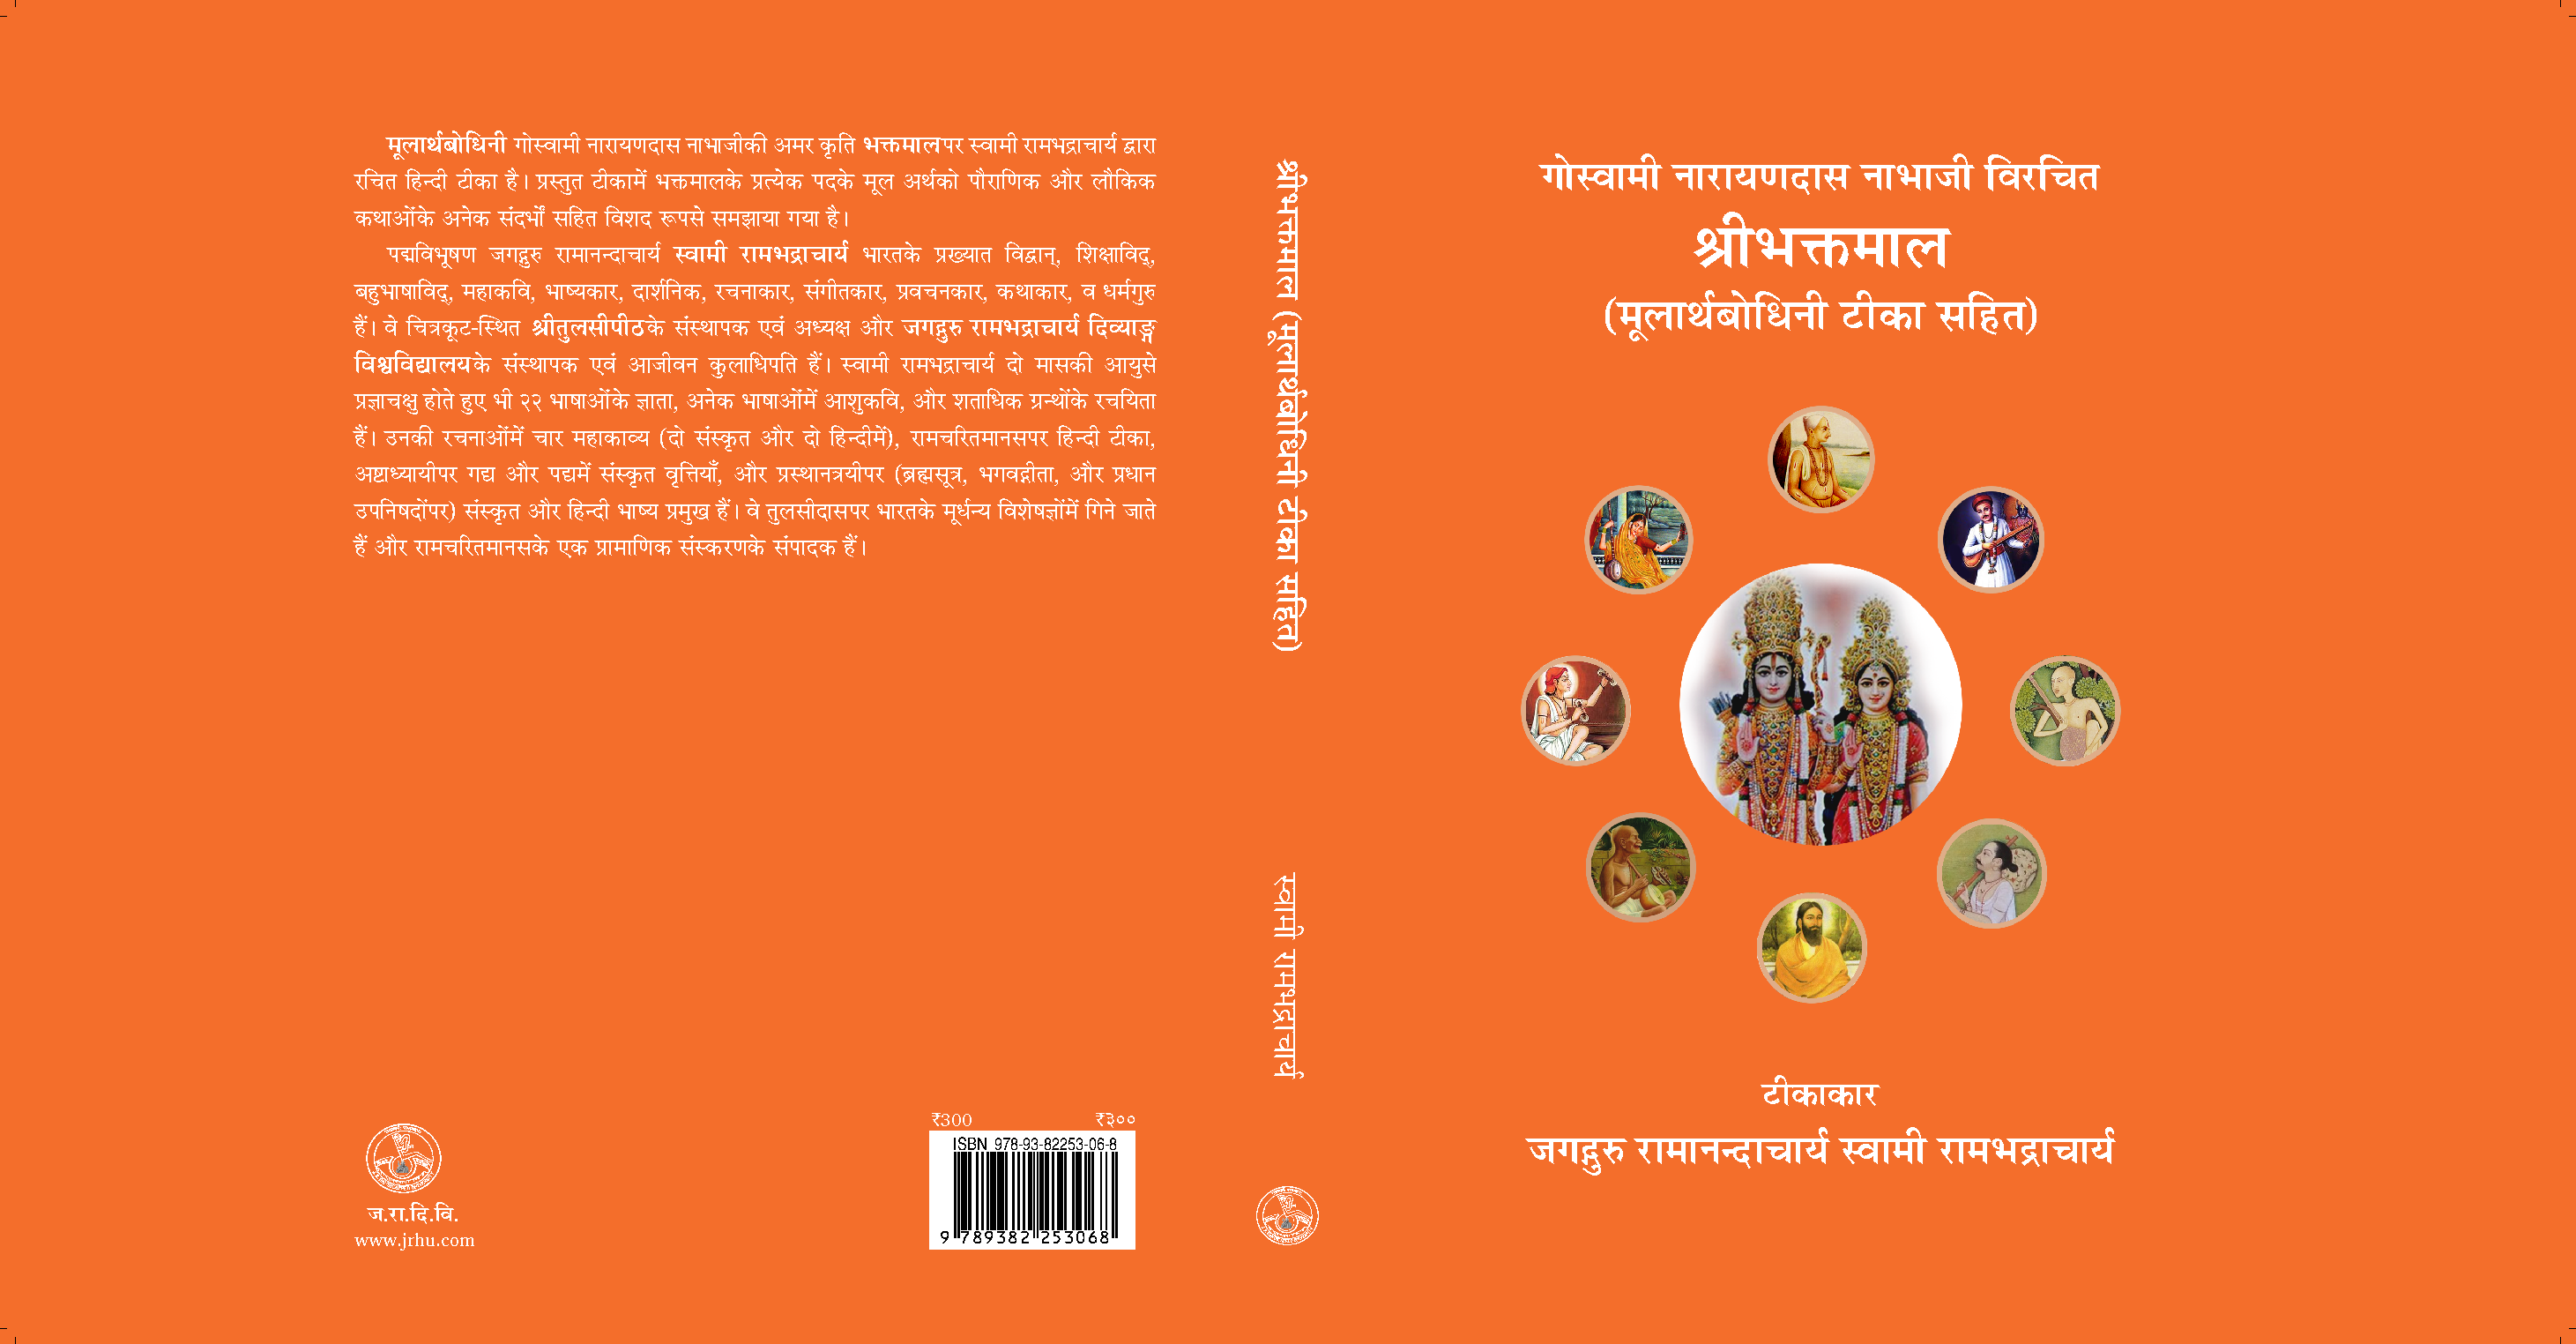
\includepdf[pages=1,trim=55.75mm 3mm 260.75mm 3mm,clip]{DustJacket}

\end{document}